\documentclass[twoside]{book}

% Packages required by doxygen
\usepackage{fixltx2e}
\usepackage{calc}
\usepackage{doxygen}
\usepackage[export]{adjustbox} % also loads graphicx
\usepackage{graphicx}
\usepackage[utf8]{inputenc}
\usepackage{makeidx}
\usepackage{multicol}
\usepackage{multirow}
\PassOptionsToPackage{warn}{textcomp}
\usepackage{textcomp}
\usepackage[nointegrals]{wasysym}
\usepackage[table]{xcolor}

% Font selection
\usepackage[T1]{fontenc}
\usepackage[scaled=.90]{helvet}
\usepackage{courier}
\usepackage{amssymb}
\usepackage{sectsty}
\renewcommand{\familydefault}{\sfdefault}
\allsectionsfont{%
  \fontseries{bc}\selectfont%
  \color{darkgray}%
}
\renewcommand{\DoxyLabelFont}{%
  \fontseries{bc}\selectfont%
  \color{darkgray}%
}
\newcommand{\+}{\discretionary{\mbox{\scriptsize$\hookleftarrow$}}{}{}}

% Page & text layout
\usepackage{geometry}
\geometry{%
  a4paper,%
  top=2.5cm,%
  bottom=2.5cm,%
  left=2.5cm,%
  right=2.5cm%
}
\tolerance=750
\hfuzz=15pt
\hbadness=750
\setlength{\emergencystretch}{15pt}
\setlength{\parindent}{0cm}
\setlength{\parskip}{3ex plus 2ex minus 2ex}
\makeatletter
\renewcommand{\paragraph}{%
  \@startsection{paragraph}{4}{0ex}{-1.0ex}{1.0ex}{%
    \normalfont\normalsize\bfseries\SS@parafont%
  }%
}
\renewcommand{\subparagraph}{%
  \@startsection{subparagraph}{5}{0ex}{-1.0ex}{1.0ex}{%
    \normalfont\normalsize\bfseries\SS@subparafont%
  }%
}
\makeatother

% Headers & footers
\usepackage{fancyhdr}
\pagestyle{fancyplain}
\fancyhead[LE]{\fancyplain{}{\bfseries\thepage}}
\fancyhead[CE]{\fancyplain{}{}}
\fancyhead[RE]{\fancyplain{}{\bfseries\leftmark}}
\fancyhead[LO]{\fancyplain{}{\bfseries\rightmark}}
\fancyhead[CO]{\fancyplain{}{}}
\fancyhead[RO]{\fancyplain{}{\bfseries\thepage}}
\fancyfoot[LE]{\fancyplain{}{}}
\fancyfoot[CE]{\fancyplain{}{}}
\fancyfoot[RE]{\fancyplain{}{\bfseries\scriptsize Generated by Doxygen }}
\fancyfoot[LO]{\fancyplain{}{\bfseries\scriptsize Generated by Doxygen }}
\fancyfoot[CO]{\fancyplain{}{}}
\fancyfoot[RO]{\fancyplain{}{}}
\renewcommand{\footrulewidth}{0.4pt}
\renewcommand{\chaptermark}[1]{%
  \markboth{#1}{}%
}
\renewcommand{\sectionmark}[1]{%
  \markright{\thesection\ #1}%
}

% Indices & bibliography
\usepackage{natbib}
\usepackage[titles]{tocloft}
\setcounter{tocdepth}{3}
\setcounter{secnumdepth}{5}
\makeindex

% Hyperlinks (required, but should be loaded last)
\usepackage{ifpdf}
\ifpdf
  \usepackage[pdftex,pagebackref=true]{hyperref}
\else
  \usepackage[ps2pdf,pagebackref=true]{hyperref}
\fi
\hypersetup{%
  colorlinks=true,%
  linkcolor=blue,%
  citecolor=blue,%
  unicode%
}

% Custom commands
\newcommand{\clearemptydoublepage}{%
  \newpage{\pagestyle{empty}\cleardoublepage}%
}

\usepackage{caption}
\captionsetup{labelsep=space,justification=centering,font={bf},singlelinecheck=off,skip=4pt,position=top}

%===== C O N T E N T S =====

\begin{document}

% Titlepage & ToC
\hypersetup{pageanchor=false,
             bookmarksnumbered=true,
             pdfencoding=unicode
            }
\pagenumbering{alph}
\begin{titlepage}
\vspace*{7cm}
\begin{center}%
{\Large L\+C\+OM T4\+G10 }\\
\vspace*{1cm}
{\large Generated by Doxygen 1.8.14}\\
\end{center}
\end{titlepage}
\clearemptydoublepage
\pagenumbering{roman}
\tableofcontents
\clearemptydoublepage
\pagenumbering{arabic}
\hypersetup{pageanchor=true}

%--- Begin generated contents ---
\chapter{Module Index}
\section{Modules}
Here is a list of all modules\+:\begin{DoxyCompactList}
\item \contentsline{section}{bitmap}{\pageref{group__bitmap}}{}
\item \contentsline{section}{bitmaps}{\pageref{group__bitmaps}}{}
\item \contentsline{section}{canvas}{\pageref{group__canvas}}{}
\item \contentsline{section}{clock}{\pageref{group__clock}}{}
\item \contentsline{section}{emote}{\pageref{group__emote}}{}
\item \contentsline{section}{event}{\pageref{group__event}}{}
\item \contentsline{section}{flappy}{\pageref{group__flappy}}{}
\item \contentsline{section}{game\+\_\+info}{\pageref{group__game__info}}{}
\item \contentsline{section}{game\+\_\+state}{\pageref{group__game__state}}{}
\item \contentsline{section}{i8042}{\pageref{group__i8042}}{}
\item \contentsline{section}{i8254}{\pageref{group__i8254}}{}
\item \contentsline{section}{interrupts}{\pageref{group__interrupts}}{}
\item \contentsline{section}{keyboard}{\pageref{group__keyboard}}{}
\item \contentsline{section}{layer}{\pageref{group__layer}}{}
\item \contentsline{section}{mouse}{\pageref{group__mouse}}{}
\item \contentsline{section}{pengoo}{\pageref{group__pengoo}}{}
\item \contentsline{section}{proj}{\pageref{group__proj}}{}
\item \contentsline{section}{queue}{\pageref{group__queue}}{}
\item \contentsline{section}{rtc}{\pageref{group__rtc}}{}
\item \contentsline{section}{snake}{\pageref{group__snake}}{}
\item \contentsline{section}{sprite}{\pageref{group__sprite}}{}
\item \contentsline{section}{textbox}{\pageref{group__textbox}}{}
\item \contentsline{section}{timer}{\pageref{group__timer}}{}
\item \contentsline{section}{uart}{\pageref{group__uart}}{}
\item \contentsline{section}{uart\+\_\+protocol}{\pageref{group__uart__protocol}}{}
\item \contentsline{section}{uart\+\_\+wordgame}{\pageref{group__uart__wordgame}}{}
\item \contentsline{section}{vbe}{\pageref{group__vbe}}{}
\item \contentsline{section}{video}{\pageref{group__video}}{}
\item \contentsline{section}{wordpicker}{\pageref{group__wordpicker}}{}
\end{DoxyCompactList}

\chapter{Class Index}
\section{Class List}
Here are the classes, structs, unions and interfaces with brief descriptions\+:\begin{DoxyCompactList}
\item\contentsline{section}{\mbox{\hyperlink{struct_bird}{Bird}} \\*Structure that represents the controlled object in the minigame }{\pageref{struct_bird}}{}
\item\contentsline{section}{\mbox{\hyperlink{struct_bitmap}{Bitmap}} \\*Represents a \mbox{\hyperlink{struct_bitmap}{Bitmap}} }{\pageref{struct_bitmap}}{}
\item\contentsline{section}{\mbox{\hyperlink{struct_bitmap_file_header}{Bitmap\+File\+Header}} \\*Represents a bitmap file header }{\pageref{struct_bitmap_file_header}}{}
\item\contentsline{section}{\mbox{\hyperlink{struct_bitmap_info_header}{Bitmap\+Info\+Header}} \\*Represents a bitmap info header }{\pageref{struct_bitmap_info_header}}{}
\item\contentsline{section}{\mbox{\hyperlink{struct_button}{Button}} \\*Represents a button, which can be pressed by a cursor }{\pageref{struct_button}}{}
\item\contentsline{section}{\mbox{\hyperlink{struct_canvas}{Canvas}} \\*Represents a canvas to draw on }{\pageref{struct_canvas}}{}
\item\contentsline{section}{\mbox{\hyperlink{structcolor}{color}} \\*Represents a pixel in direct color mode }{\pageref{structcolor}}{}
\item\contentsline{section}{\mbox{\hyperlink{struct_date}{Date}} \\*Represents a complete date }{\pageref{struct_date}}{}
\item\contentsline{section}{\mbox{\hyperlink{struct_drawing_state}{Drawing\+State}} \\*Contains information about the drawing state }{\pageref{struct_drawing_state}}{}
\item\contentsline{section}{\mbox{\hyperlink{struct_event__t}{Event\+\_\+t}} \\*Represents an event }{\pageref{struct_event__t}}{}
\item\contentsline{section}{\mbox{\hyperlink{struct_flappy_tube}{Flappy\+Tube}} \\*Represents an obstacle in the minigame }{\pageref{struct_flappy_tube}}{}
\item\contentsline{section}{\mbox{\hyperlink{struct_hitbox}{Hitbox}} \\*Rectangle shape representing an area belonging to a sprite }{\pageref{struct_hitbox}}{}
\item\contentsline{section}{\mbox{\hyperlink{struct_idle_sprite}{Idle\+Sprite}} \\*Same as a regular sprite, except G\+R\+E\+EN is always replaced by its color when drawn, cannot be moved, and is not necessarily drawn on top of all the other elements. (It\textquotesingle{}s on a layer) }{\pageref{struct_idle_sprite}}{}
\item\contentsline{section}{\mbox{\hyperlink{struct_keyboard_event}{Keyboard\+Event}} \\*Represents a keyboard event }{\pageref{struct_keyboard_event}}{}
\item\contentsline{section}{\mbox{\hyperlink{struct_layer}{Layer}} \\*Represents a layer, which may be under, or on top of other layers }{\pageref{struct_layer}}{}
\item\contentsline{section}{\mbox{\hyperlink{struct_mini___date}{Mini\+\_\+\+Date}} \\*Represents a hour/min/sec }{\pageref{struct_mini___date}}{}
\item\contentsline{section}{\mbox{\hyperlink{struct_mouse_event}{Mouse\+Event}} \\*Represents a mouse event }{\pageref{struct_mouse_event}}{}
\item\contentsline{section}{\mbox{\hyperlink{struct_notification}{Notification}} \\*Represents a received interrupt notification }{\pageref{struct_notification}}{}
\item\contentsline{section}{\mbox{\hyperlink{struct_obstacle}{Obstacle}} \\*Represents a snake obstacle }{\pageref{struct_obstacle}}{}
\item\contentsline{section}{\mbox{\hyperlink{struct_powerup}{Powerup}} \\*Represents a snake powerup }{\pageref{struct_powerup}}{}
\item\contentsline{section}{\mbox{\hyperlink{struct_queue}{Queue}} \\*Represents a queue }{\pageref{struct_queue}}{}
\item\contentsline{section}{\mbox{\hyperlink{struct_slider}{Slider}} \\*Represents a slider, whose handle the user can drag with the mouse }{\pageref{struct_slider}}{}
\item\contentsline{section}{\mbox{\hyperlink{struct_snake}{Snake}} \\*Structure that represents the controlled object in the snake minigame }{\pageref{struct_snake}}{}
\item\contentsline{section}{\mbox{\hyperlink{struct_snake_arena}{Snake\+Arena}} \\*Represents an arena where the rainbow snake can move on }{\pageref{struct_snake_arena}}{}
\item\contentsline{section}{\mbox{\hyperlink{struct_snake_decoy}{Snake\+Decoy}} \\*Represent a snake decoy, used for when the snake multiplies }{\pageref{struct_snake_decoy}}{}
\item\contentsline{section}{\mbox{\hyperlink{struct_sprite}{Sprite}} \\*Represents a 2D sprite }{\pageref{struct_sprite}}{}
\item\contentsline{section}{\mbox{\hyperlink{struct_text_box}{Text\+Box}} \\*Represents a text box, which can be used to display text }{\pageref{struct_text_box}}{}
\item\contentsline{section}{\mbox{\hyperlink{struct_timer_event}{Timer\+Event}} \\*Represents a timer event }{\pageref{struct_timer_event}}{}
\item\contentsline{section}{\mbox{\hyperlink{struct_u_a_r_t___int___info}{U\+A\+R\+T\+\_\+\+Int\+\_\+\+Info}} \\*Contains information about the received/sent information through the U\+A\+RT }{\pageref{struct_u_a_r_t___int___info}}{}
\item\contentsline{section}{\mbox{\hyperlink{struct_u_a_r_t_message}{U\+A\+R\+T\+Message}} \\*Represents a Message that is send through the serial port }{\pageref{struct_u_a_r_t_message}}{}
\item\contentsline{section}{\mbox{\hyperlink{struct_u_a_r_t_message_contents}{U\+A\+R\+T\+Message\+Contents}} \\*Structure containing possible contents for the U\+A\+RT Messages. The used elements are \char`\"{}indicated\char`\"{} by the type member }{\pageref{struct_u_a_r_t_message_contents}}{}
\item\contentsline{section}{\mbox{\hyperlink{structvbe__info__block}{vbe\+\_\+info\+\_\+block}} \\*Contains information about the V\+BE controller }{\pageref{structvbe__info__block}}{}
\end{DoxyCompactList}

\chapter{File Index}
\section{File List}
Here is a list of all files with brief descriptions\+:\begin{DoxyCompactList}
\item\contentsline{section}{\mbox{\hyperlink{bitmap_8c}{bitmap.\+c}} }{\pageref{bitmap_8c}}{}
\item\contentsline{section}{\mbox{\hyperlink{bitmap_8h}{bitmap.\+h}} }{\pageref{bitmap_8h}}{}
\item\contentsline{section}{\mbox{\hyperlink{bitmaps_8c}{bitmaps.\+c}} }{\pageref{bitmaps_8c}}{}
\item\contentsline{section}{\mbox{\hyperlink{bitmaps_8h}{bitmaps.\+h}} }{\pageref{bitmaps_8h}}{}
\item\contentsline{section}{\mbox{\hyperlink{canvas_8c}{canvas.\+c}} }{\pageref{canvas_8c}}{}
\item\contentsline{section}{\mbox{\hyperlink{canvas_8h}{canvas.\+h}} }{\pageref{canvas_8h}}{}
\item\contentsline{section}{\mbox{\hyperlink{clock_8c}{clock.\+c}} }{\pageref{clock_8c}}{}
\item\contentsline{section}{\mbox{\hyperlink{clock_8h}{clock.\+h}} }{\pageref{clock_8h}}{}
\item\contentsline{section}{\mbox{\hyperlink{emote_8c}{emote.\+c}} }{\pageref{emote_8c}}{}
\item\contentsline{section}{\mbox{\hyperlink{emote_8h}{emote.\+h}} }{\pageref{emote_8h}}{}
\item\contentsline{section}{\mbox{\hyperlink{event_8c}{event.\+c}} }{\pageref{event_8c}}{}
\item\contentsline{section}{\mbox{\hyperlink{event_8h}{event.\+h}} }{\pageref{event_8h}}{}
\item\contentsline{section}{\mbox{\hyperlink{flappy_8c}{flappy.\+c}} }{\pageref{flappy_8c}}{}
\item\contentsline{section}{\mbox{\hyperlink{flappy_8h}{flappy.\+h}} }{\pageref{flappy_8h}}{}
\item\contentsline{section}{\mbox{\hyperlink{game__info_8c}{game\+\_\+info.\+c}} }{\pageref{game__info_8c}}{}
\item\contentsline{section}{\mbox{\hyperlink{game__info_8h}{game\+\_\+info.\+h}} }{\pageref{game__info_8h}}{}
\item\contentsline{section}{\mbox{\hyperlink{game__state_8c}{game\+\_\+state.\+c}} }{\pageref{game__state_8c}}{}
\item\contentsline{section}{\mbox{\hyperlink{game__state_8h}{game\+\_\+state.\+h}} }{\pageref{game__state_8h}}{}
\item\contentsline{section}{\mbox{\hyperlink{i8042_8h}{i8042.\+h}} }{\pageref{i8042_8h}}{}
\item\contentsline{section}{\mbox{\hyperlink{i8254_8h}{i8254.\+h}} }{\pageref{i8254_8h}}{}
\item\contentsline{section}{\mbox{\hyperlink{interrupts_8c}{interrupts.\+c}} }{\pageref{interrupts_8c}}{}
\item\contentsline{section}{\mbox{\hyperlink{interrupts_8h}{interrupts.\+h}} }{\pageref{interrupts_8h}}{}
\item\contentsline{section}{\mbox{\hyperlink{keyboard_8c}{keyboard.\+c}} }{\pageref{keyboard_8c}}{}
\item\contentsline{section}{\mbox{\hyperlink{keyboard_8h}{keyboard.\+h}} }{\pageref{keyboard_8h}}{}
\item\contentsline{section}{\mbox{\hyperlink{layer_8c}{layer.\+c}} }{\pageref{layer_8c}}{}
\item\contentsline{section}{\mbox{\hyperlink{layer_8h}{layer.\+h}} }{\pageref{layer_8h}}{}
\item\contentsline{section}{\mbox{\hyperlink{mouse_8c}{mouse.\+c}} }{\pageref{mouse_8c}}{}
\item\contentsline{section}{\mbox{\hyperlink{mouse_8h}{mouse.\+h}} }{\pageref{mouse_8h}}{}
\item\contentsline{section}{\mbox{\hyperlink{pengoo_8c}{pengoo.\+c}} }{\pageref{pengoo_8c}}{}
\item\contentsline{section}{\mbox{\hyperlink{pengoo_8h}{pengoo.\+h}} }{\pageref{pengoo_8h}}{}
\item\contentsline{section}{\mbox{\hyperlink{proj_8c}{proj.\+c}} }{\pageref{proj_8c}}{}
\item\contentsline{section}{\mbox{\hyperlink{queue_8c}{queue.\+c}} }{\pageref{queue_8c}}{}
\item\contentsline{section}{\mbox{\hyperlink{queue_8h}{queue.\+h}} }{\pageref{queue_8h}}{}
\item\contentsline{section}{\mbox{\hyperlink{rtc_8c}{rtc.\+c}} }{\pageref{rtc_8c}}{}
\item\contentsline{section}{\mbox{\hyperlink{rtc_8h}{rtc.\+h}} }{\pageref{rtc_8h}}{}
\item\contentsline{section}{\mbox{\hyperlink{snake_8c}{snake.\+c}} }{\pageref{snake_8c}}{}
\item\contentsline{section}{\mbox{\hyperlink{snake_8h}{snake.\+h}} }{\pageref{snake_8h}}{}
\item\contentsline{section}{\mbox{\hyperlink{sprite_8c}{sprite.\+c}} }{\pageref{sprite_8c}}{}
\item\contentsline{section}{\mbox{\hyperlink{sprite_8h}{sprite.\+h}} }{\pageref{sprite_8h}}{}
\item\contentsline{section}{\mbox{\hyperlink{textbox_8c}{textbox.\+c}} }{\pageref{textbox_8c}}{}
\item\contentsline{section}{\mbox{\hyperlink{textbox_8h}{textbox.\+h}} }{\pageref{textbox_8h}}{}
\item\contentsline{section}{\mbox{\hyperlink{timer_8c}{timer.\+c}} }{\pageref{timer_8c}}{}
\item\contentsline{section}{\mbox{\hyperlink{timer_8h}{timer.\+h}} }{\pageref{timer_8h}}{}
\item\contentsline{section}{\mbox{\hyperlink{uart_8c}{uart.\+c}} }{\pageref{uart_8c}}{}
\item\contentsline{section}{\mbox{\hyperlink{uart_8h}{uart.\+h}} }{\pageref{uart_8h}}{}
\item\contentsline{section}{\mbox{\hyperlink{uart__protocol_8c}{uart\+\_\+protocol.\+c}} }{\pageref{uart__protocol_8c}}{}
\item\contentsline{section}{\mbox{\hyperlink{uart__protocol_8h}{uart\+\_\+protocol.\+h}} }{\pageref{uart__protocol_8h}}{}
\item\contentsline{section}{\mbox{\hyperlink{uart__wordgame_8c}{uart\+\_\+wordgame.\+c}} }{\pageref{uart__wordgame_8c}}{}
\item\contentsline{section}{\mbox{\hyperlink{uart__wordgame_8h}{uart\+\_\+wordgame.\+h}} }{\pageref{uart__wordgame_8h}}{}
\item\contentsline{section}{\mbox{\hyperlink{vbe_8c}{vbe.\+c}} }{\pageref{vbe_8c}}{}
\item\contentsline{section}{\mbox{\hyperlink{vbe_8h}{vbe.\+h}} }{\pageref{vbe_8h}}{}
\item\contentsline{section}{\mbox{\hyperlink{video_8c}{video.\+c}} }{\pageref{video_8c}}{}
\item\contentsline{section}{\mbox{\hyperlink{video_8h}{video.\+h}} }{\pageref{video_8h}}{}
\item\contentsline{section}{\mbox{\hyperlink{wordpicker_8c}{wordpicker.\+c}} }{\pageref{wordpicker_8c}}{}
\item\contentsline{section}{\mbox{\hyperlink{wordpicker_8h}{wordpicker.\+h}} }{\pageref{wordpicker_8h}}{}
\end{DoxyCompactList}

\chapter{Module Documentation}
\hypertarget{group__bitmap}{}\section{bitmap}
\label{group__bitmap}\index{bitmap@{bitmap}}
\subsection*{Classes}
\begin{DoxyCompactItemize}
\item 
struct \mbox{\hyperlink{struct_bitmap_file_header}{Bitmap\+File\+Header}}
\begin{DoxyCompactList}\small\item\em Represents a bitmap file header. \end{DoxyCompactList}\item 
struct \mbox{\hyperlink{struct_bitmap_info_header}{Bitmap\+Info\+Header}}
\begin{DoxyCompactList}\small\item\em Represents a bitmap info header. \end{DoxyCompactList}\item 
struct \mbox{\hyperlink{struct_bitmap}{Bitmap}}
\begin{DoxyCompactList}\small\item\em Represents a \mbox{\hyperlink{struct_bitmap}{Bitmap}}. \end{DoxyCompactList}\end{DoxyCompactItemize}
\subsection*{Functions}
\begin{DoxyCompactItemize}
\item 
void \mbox{\hyperlink{group__bitmap_gacc8595ed81c710cecebe95f04db413fe}{save\+Bitmap}} (char $\ast$path, unsigned int width, unsigned int height, char $\ast$address)
\begin{DoxyCompactList}\small\item\em Saves a bitmap in a .bmp file. \end{DoxyCompactList}\item 
\mbox{\hyperlink{struct_bitmap}{Bitmap}} $\ast$ \mbox{\hyperlink{group__bitmap_ga627d64d58e9bf487fb6e326ea65df57b}{load\+Bitmap}} (const char $\ast$folder\+Path, const char $\ast$filename)
\begin{DoxyCompactList}\small\item\em Loads a .bmp file. \end{DoxyCompactList}\item 
\mbox{\hyperlink{struct_bitmap}{Bitmap}} $\ast$ \mbox{\hyperlink{group__bitmap_ga3f8f5ad40944f2db40792d7c4fe5b96e}{load\+Bitmap\+Section}} (\mbox{\hyperlink{struct_bitmap}{Bitmap}} $\ast$bitmap, uint16\+\_\+t x, uint16\+\_\+t y, uint16\+\_\+t width, uint16\+\_\+t height)
\begin{DoxyCompactList}\small\item\em Copies part of a bitmap from a given bitmap to another bitmap. \end{DoxyCompactList}\item 
\mbox{\hyperlink{struct_bitmap}{Bitmap}} $\ast$ \mbox{\hyperlink{group__bitmap_gaa19cec779e8cbaf053f3efc749c20c37}{resize\+Bitmap}} (\mbox{\hyperlink{struct_bitmap}{Bitmap}} $\ast$bitmap, uint16\+\_\+t factor)
\begin{DoxyCompactList}\small\item\em Resizes a bitmap by a given factor. \end{DoxyCompactList}\item 
void \mbox{\hyperlink{group__bitmap_ga37e42f0583efd18e7efa5a036798539e}{draw\+\_\+bitmap}} (\mbox{\hyperlink{struct_bitmap}{Bitmap}} $\ast$bmp, int x, int y)
\begin{DoxyCompactList}\small\item\em Draws a bitmap on the screen. \end{DoxyCompactList}\item 
void \mbox{\hyperlink{group__bitmap_ga0a2714359072f1a1b3f361c89e30be52}{draw\+\_\+bitmap\+\_\+color}} (\mbox{\hyperlink{struct_bitmap}{Bitmap}} $\ast$bmp, int x, int y, uint32\+\_\+t new\+\_\+color)
\begin{DoxyCompactList}\small\item\em Draws a bitmap on the screen, replacing every G\+R\+E\+EN pixel with another color. \end{DoxyCompactList}\item 
void \mbox{\hyperlink{group__bitmap_ga12d1b6c1fa206ba89cf45d23f6679657}{draw\+\_\+bitmap\+\_\+transp}} (\mbox{\hyperlink{struct_bitmap}{Bitmap}} $\ast$bmp, int x, int y, double alpha)
\begin{DoxyCompactList}\small\item\em Draws a bitmap on the screen, allowing the caller to use transparency. The color B\+L\+A\+CK ignores transparency values. \end{DoxyCompactList}\item 
void \mbox{\hyperlink{group__bitmap_ga3c405395b542105657c9811e99c56da4}{draw\+\_\+bitmap\+\_\+rotate}} (\mbox{\hyperlink{struct_bitmap}{Bitmap}} $\ast$bmp, int x, int y, double angle)
\begin{DoxyCompactList}\small\item\em Draws a bitmap on the screen, rotated by an angle. \end{DoxyCompactList}\item 
uint32\+\_\+t \mbox{\hyperlink{group__bitmap_gad73cdf3b48e5ca2e43ef1fbdd5b061b9}{get\+\_\+bitmap\+\_\+color}} (\mbox{\hyperlink{struct_bitmap}{Bitmap}} $\ast$bmp, uint16\+\_\+t x, uint16\+\_\+t y)
\begin{DoxyCompactList}\small\item\em Gets the color of a certain bitmap pixel. \end{DoxyCompactList}\item 
void \mbox{\hyperlink{group__bitmap_ga08c1d4f4fff81df260d979ea8fc1aa61}{delete\+Bitmap}} (\mbox{\hyperlink{struct_bitmap}{Bitmap}} $\ast$bmp)
\begin{DoxyCompactList}\small\item\em Deletes a bitmap, freeing the used memory. \end{DoxyCompactList}\item 
bool \mbox{\hyperlink{group__bitmap_ga4b5b3aefecdb54bfdadbe4995b979c7f}{is\+\_\+transparent}} (uint32\+\_\+t \mbox{\hyperlink{structcolor}{color}})
\begin{DoxyCompactList}\small\item\em Checks if a color is transparent (M\+A\+G\+E\+N\+TA) \end{DoxyCompactList}\end{DoxyCompactItemize}
\subsection*{Variables}
\begin{DoxyCompactItemize}
\item 
unsigned short int \mbox{\hyperlink{group__bitmap_ga0206e64e29930b0594e714cbdf8090f0}{Bitmap\+File\+Header\+::type}}
\begin{DoxyCompactList}\small\item\em specifies the file type \end{DoxyCompactList}\item 
unsigned int \mbox{\hyperlink{group__bitmap_ga0dcad71d9b17783c4d296c2c6d00ede0}{Bitmap\+File\+Header\+::size}}
\begin{DoxyCompactList}\small\item\em specifies the size in bytes of the bitmap file \end{DoxyCompactList}\item 
unsigned short \mbox{\hyperlink{group__bitmap_ga16d8cfe2edb9d109cea44ab94d1b701a}{Bitmap\+File\+Header\+::reserved1}}
\begin{DoxyCompactList}\small\item\em reserved; must be 0 \end{DoxyCompactList}\item 
unsigned short int \mbox{\hyperlink{group__bitmap_ga24130729dee5b8b9c1bd45f0a73c9a9d}{Bitmap\+File\+Header\+::reserved2}}
\begin{DoxyCompactList}\small\item\em reserved; must be 0 \end{DoxyCompactList}\item 
unsigned int \mbox{\hyperlink{group__bitmap_ga26ed598693b100ffd9e29c4dc77f3d92}{Bitmap\+File\+Header\+::offset}}
\begin{DoxyCompactList}\small\item\em specifies the offset in bytes from the bitmapfileheader to the bitmap bits \end{DoxyCompactList}\item 
unsigned int \mbox{\hyperlink{group__bitmap_ga411fa70f6547a0360b33edcd3273d169}{Bitmap\+Info\+Header\+::size}}
\begin{DoxyCompactList}\small\item\em specifies the number of bytes required by the struct \end{DoxyCompactList}\item 
int \mbox{\hyperlink{group__bitmap_gac2034cfbada460819beed1ee24581c5d}{Bitmap\+Info\+Header\+::width}}
\begin{DoxyCompactList}\small\item\em specifies width in pixels \end{DoxyCompactList}\item 
int \mbox{\hyperlink{group__bitmap_gaaa1d31efc13210020a38d435e4961df9}{Bitmap\+Info\+Header\+::height}}
\begin{DoxyCompactList}\small\item\em specifies height in pixels \end{DoxyCompactList}\item 
unsigned short \mbox{\hyperlink{group__bitmap_ga9925e97e8bbc6b797afe2d22fbab45d6}{Bitmap\+Info\+Header\+::planes}}
\begin{DoxyCompactList}\small\item\em specifies the number of color planes, must be 1 \end{DoxyCompactList}\item 
unsigned short \mbox{\hyperlink{group__bitmap_ga2a1eb136325c8cb16aeeb7108703702f}{Bitmap\+Info\+Header\+::bits\+Per\+Pixel}}
\begin{DoxyCompactList}\small\item\em specifies the number of bit per pixel \end{DoxyCompactList}\item 
unsigned int \mbox{\hyperlink{group__bitmap_ga87fb38b0fe68db4bed899b9733d1b7e9}{Bitmap\+Info\+Header\+::compression}}
\begin{DoxyCompactList}\small\item\em specifies the type of compression \end{DoxyCompactList}\item 
unsigned int \mbox{\hyperlink{group__bitmap_ga79bc984a7fd1c0f00ede6aa09143939f}{Bitmap\+Info\+Header\+::image\+Size}}
\begin{DoxyCompactList}\small\item\em size of image in bytes \end{DoxyCompactList}\item 
int \mbox{\hyperlink{group__bitmap_ga391cf1da75d16aee3b6539ccf5b29300}{Bitmap\+Info\+Header\+::x\+Resolution}}
\begin{DoxyCompactList}\small\item\em number of pixels per meter in x axis \end{DoxyCompactList}\item 
int \mbox{\hyperlink{group__bitmap_gaf2fadf9c216cc9f3ce401096e35be1b7}{Bitmap\+Info\+Header\+::y\+Resolution}}
\begin{DoxyCompactList}\small\item\em number of pixels per meter in y axis \end{DoxyCompactList}\item 
unsigned int \mbox{\hyperlink{group__bitmap_ga4c543a08d1b72bdda2329b426a213e2a}{Bitmap\+Info\+Header\+::n\+Colors}}
\begin{DoxyCompactList}\small\item\em number of colors used by the bitmap \end{DoxyCompactList}\item 
unsigned int \mbox{\hyperlink{group__bitmap_ga9d87941fcc414085f7361fd89818ee3f}{Bitmap\+Info\+Header\+::important\+Colors}}
\begin{DoxyCompactList}\small\item\em number of colors that are important \end{DoxyCompactList}\item 
\mbox{\hyperlink{struct_bitmap_info_header}{Bitmap\+Info\+Header}} \mbox{\hyperlink{group__bitmap_ga95c481a5ce1ff4af08cd135ca4af120b}{Bitmap\+::bitmap\+Info\+Header}}
\begin{DoxyCompactList}\small\item\em \mbox{\hyperlink{struct_bitmap}{Bitmap}} info header. \end{DoxyCompactList}\item 
char $\ast$ \mbox{\hyperlink{group__bitmap_gad3fa2b9ac8c411719d9c261f41a999f9}{Bitmap\+::bitmap\+Data}}
\begin{DoxyCompactList}\small\item\em Pointer to the pixel map buffer. \end{DoxyCompactList}\item 
unsigned int \mbox{\hyperlink{group__bitmap_gac4487f25d79f268d5bb0580e68e82b53}{Bitmap\+::bytes\+\_\+per\+\_\+pixel}}
\begin{DoxyCompactList}\small\item\em Bytes per pixel used by the bitmap. \end{DoxyCompactList}\item 
unsigned int \mbox{\hyperlink{group__bitmap_ga0ff33a06b37b2b310a499b4ef19fb490}{Bitmap\+::padding}}
\begin{DoxyCompactList}\small\item\em \mbox{\hyperlink{struct_bitmap}{Bitmap}} padding per row. \end{DoxyCompactList}\item 
unsigned int \mbox{\hyperlink{group__bitmap_ga65e6af125468dec1b3b7cf18fad3800f}{Bitmap\+::actual\+\_\+bytes\+\_\+per\+\_\+row}}
\begin{DoxyCompactList}\small\item\em Number of bytes per row (including padding) \end{DoxyCompactList}\end{DoxyCompactItemize}


\subsection{Detailed Description}
Functions used to create and manipulate B\+MP files. 

\subsection{Function Documentation}
\mbox{\Hypertarget{group__bitmap_ga08c1d4f4fff81df260d979ea8fc1aa61}\label{group__bitmap_ga08c1d4f4fff81df260d979ea8fc1aa61}} 
\index{bitmap@{bitmap}!delete\+Bitmap@{delete\+Bitmap}}
\index{delete\+Bitmap@{delete\+Bitmap}!bitmap@{bitmap}}
\subsubsection{\texorpdfstring{delete\+Bitmap()}{deleteBitmap()}}
{\footnotesize\ttfamily void delete\+Bitmap (\begin{DoxyParamCaption}\item[{\mbox{\hyperlink{struct_bitmap}{Bitmap}} $\ast$}]{bmp }\end{DoxyParamCaption})}



Deletes a bitmap, freeing the used memory. 


\begin{DoxyParams}{Parameters}
{\em bmp} & \mbox{\hyperlink{struct_bitmap}{Bitmap}} to be deleted \\
\hline
\end{DoxyParams}
Here is the caller graph for this function\+:\nopagebreak
\begin{figure}[H]
\begin{center}
\leavevmode
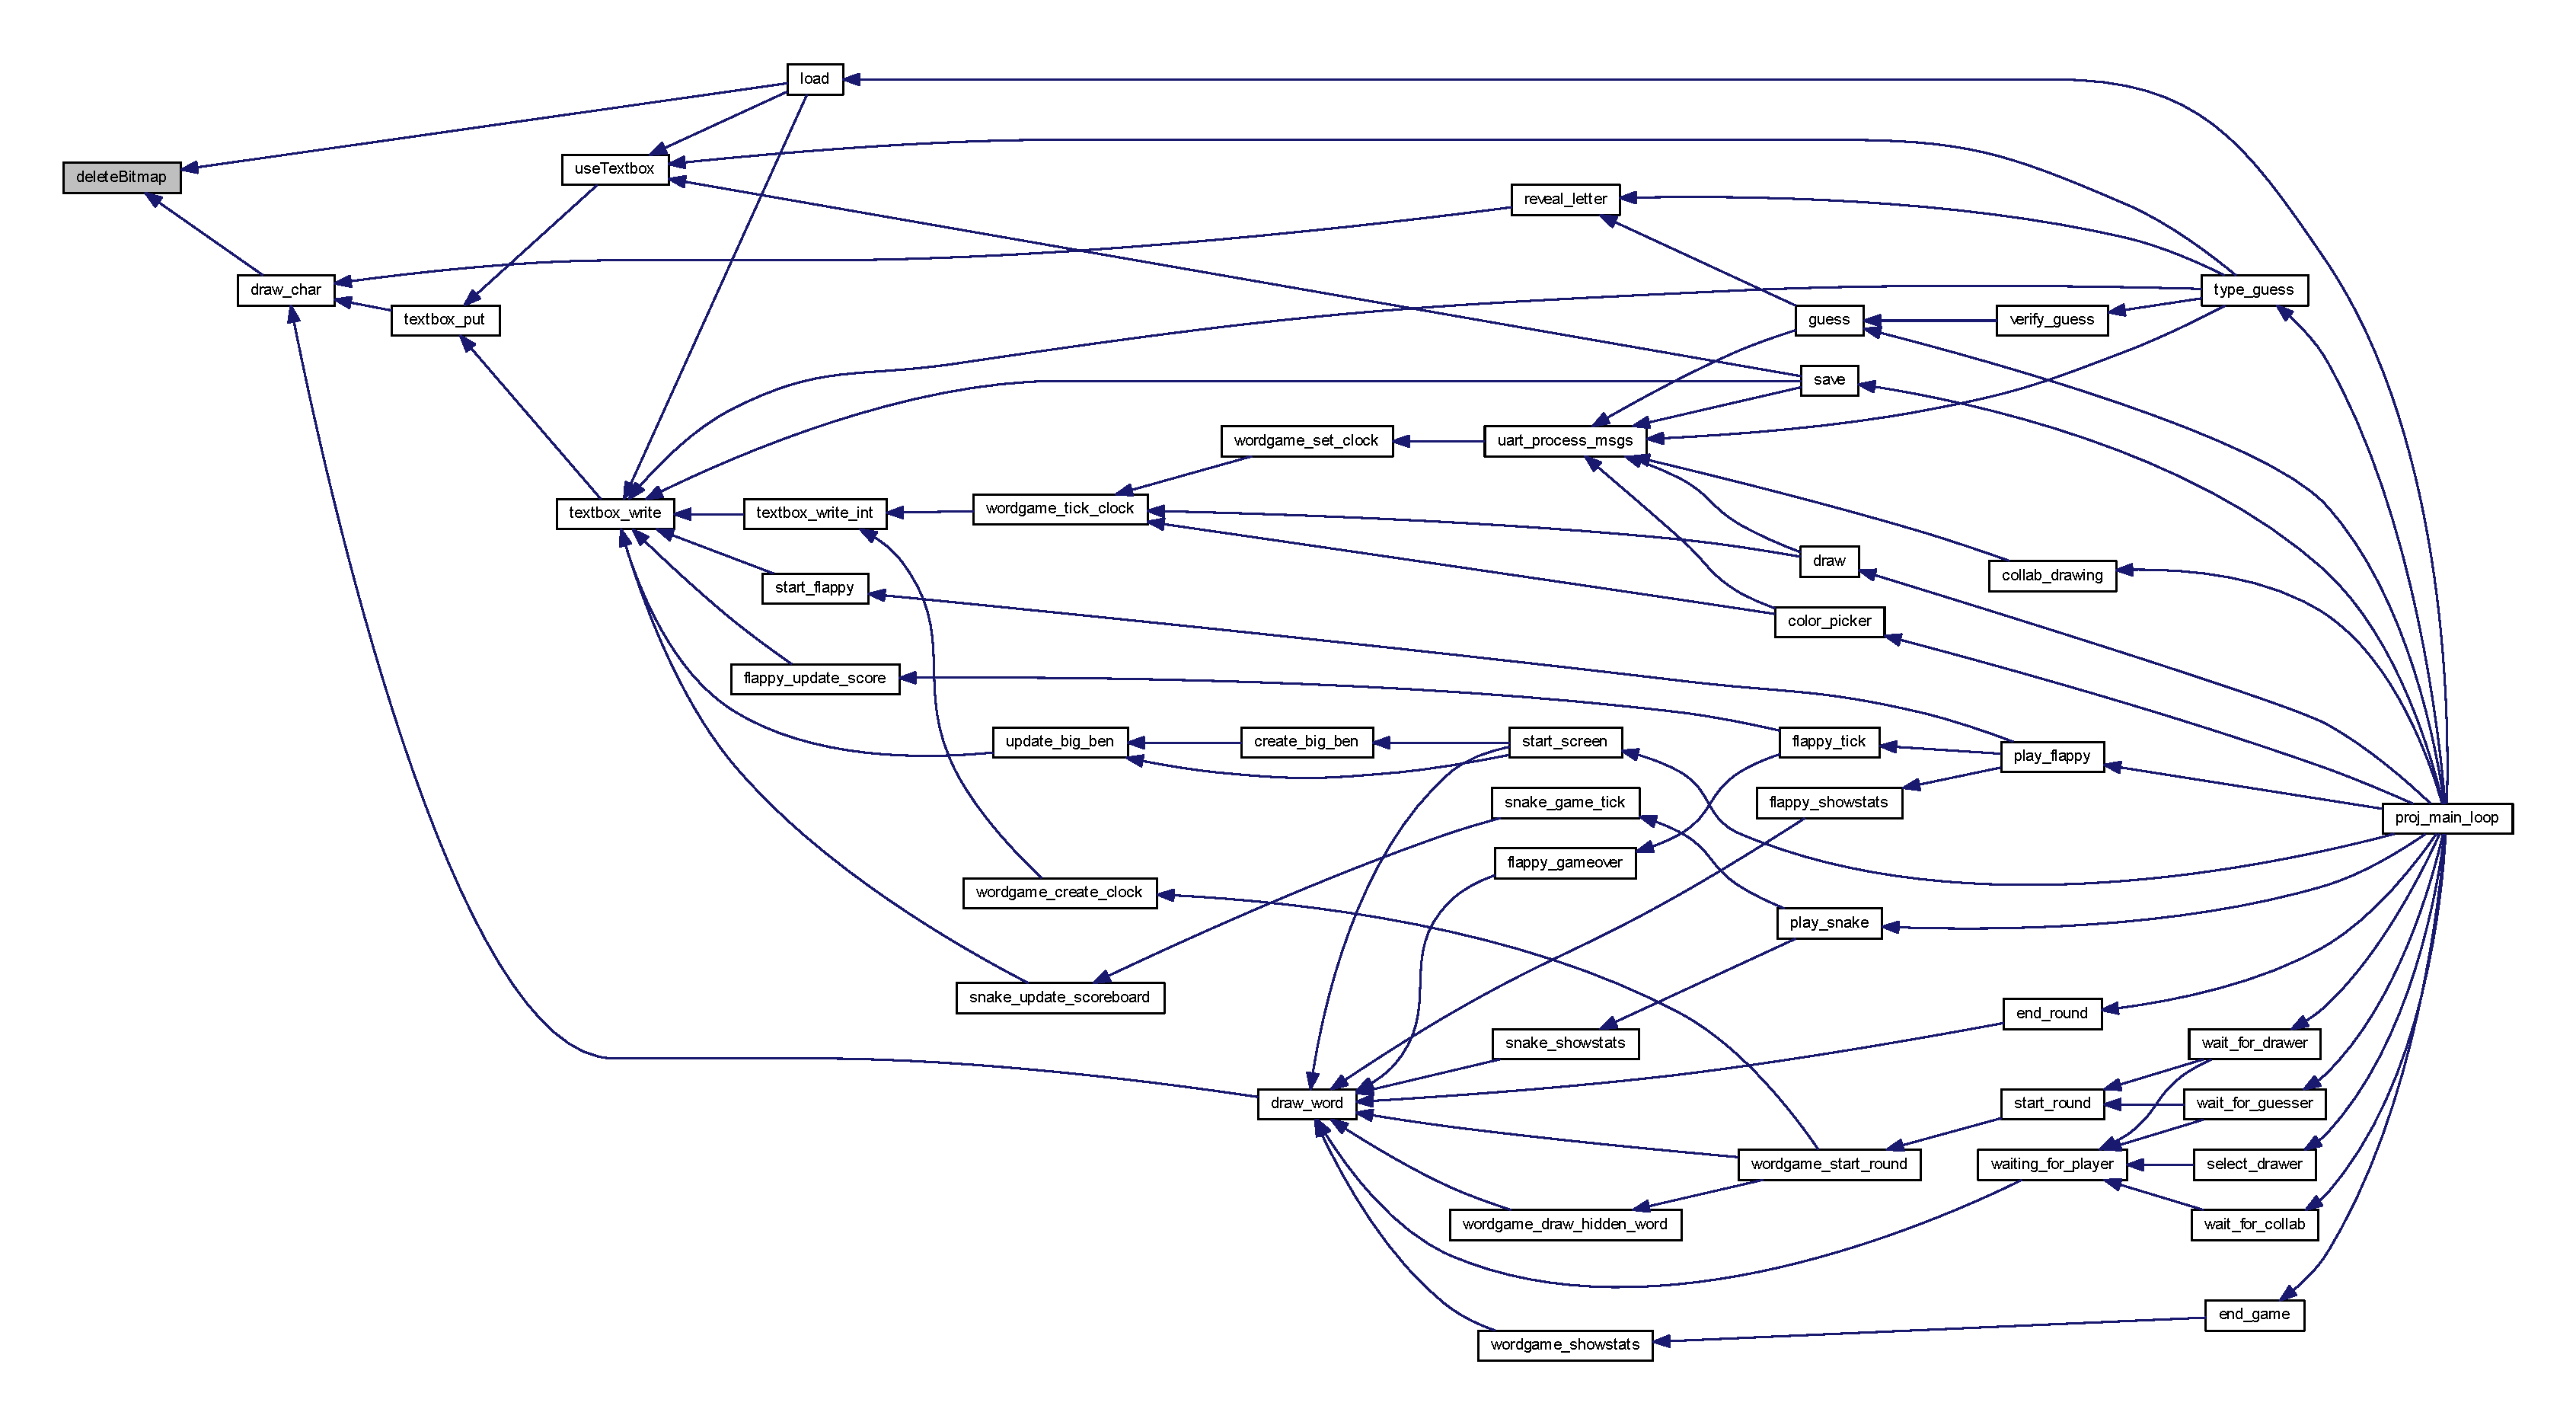
\includegraphics[width=350pt]{group__bitmap_ga08c1d4f4fff81df260d979ea8fc1aa61_icgraph}
\end{center}
\end{figure}
\mbox{\Hypertarget{group__bitmap_ga37e42f0583efd18e7efa5a036798539e}\label{group__bitmap_ga37e42f0583efd18e7efa5a036798539e}} 
\index{bitmap@{bitmap}!draw\+\_\+bitmap@{draw\+\_\+bitmap}}
\index{draw\+\_\+bitmap@{draw\+\_\+bitmap}!bitmap@{bitmap}}
\subsubsection{\texorpdfstring{draw\+\_\+bitmap()}{draw\_bitmap()}}
{\footnotesize\ttfamily void draw\+\_\+bitmap (\begin{DoxyParamCaption}\item[{\mbox{\hyperlink{struct_bitmap}{Bitmap}} $\ast$}]{bmp,  }\item[{int}]{x,  }\item[{int}]{y }\end{DoxyParamCaption})}



Draws a bitmap on the screen. 


\begin{DoxyParams}{Parameters}
{\em bmp} & Pointer to the \mbox{\hyperlink{struct_bitmap}{Bitmap}} that will be drawn \\
\hline
{\em x} & X position of the upper left corner \\
\hline
{\em y} & Y position of the upper left corner \\
\hline
\end{DoxyParams}
Here is the call graph for this function\+:\nopagebreak
\begin{figure}[H]
\begin{center}
\leavevmode
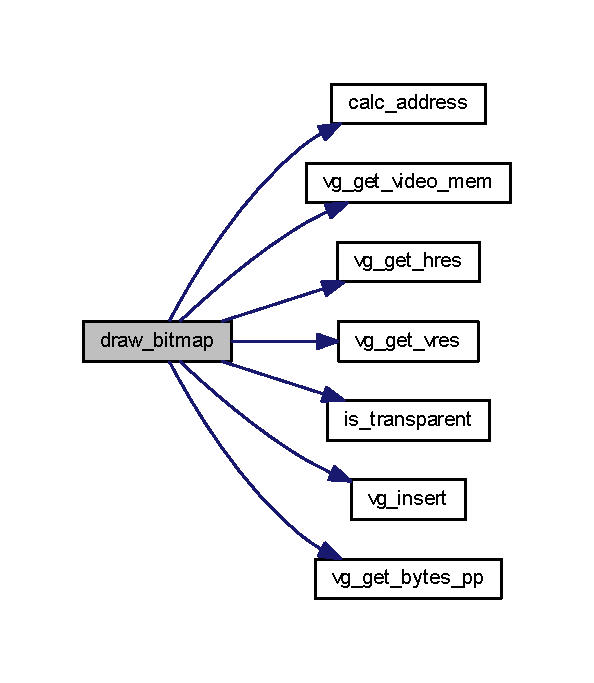
\includegraphics[width=285pt]{group__bitmap_ga37e42f0583efd18e7efa5a036798539e_cgraph}
\end{center}
\end{figure}
Here is the caller graph for this function\+:\nopagebreak
\begin{figure}[H]
\begin{center}
\leavevmode
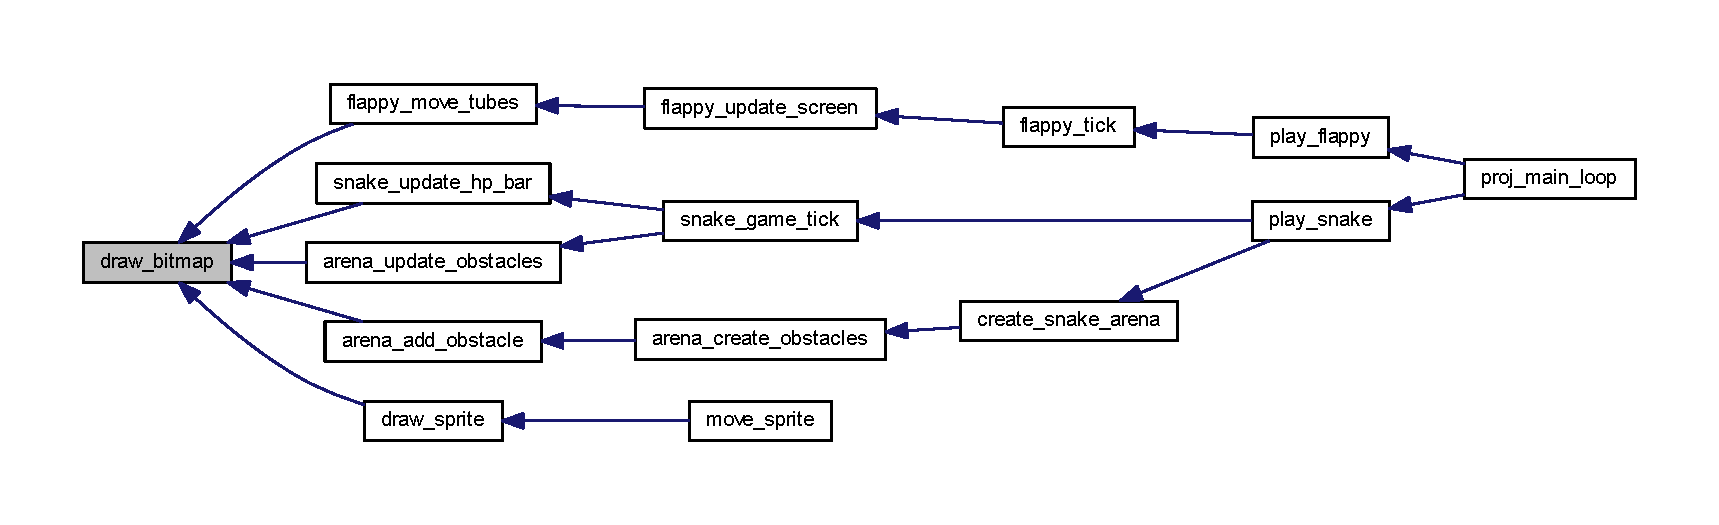
\includegraphics[width=350pt]{group__bitmap_ga37e42f0583efd18e7efa5a036798539e_icgraph}
\end{center}
\end{figure}
\mbox{\Hypertarget{group__bitmap_ga0a2714359072f1a1b3f361c89e30be52}\label{group__bitmap_ga0a2714359072f1a1b3f361c89e30be52}} 
\index{bitmap@{bitmap}!draw\+\_\+bitmap\+\_\+color@{draw\+\_\+bitmap\+\_\+color}}
\index{draw\+\_\+bitmap\+\_\+color@{draw\+\_\+bitmap\+\_\+color}!bitmap@{bitmap}}
\subsubsection{\texorpdfstring{draw\+\_\+bitmap\+\_\+color()}{draw\_bitmap\_color()}}
{\footnotesize\ttfamily void draw\+\_\+bitmap\+\_\+color (\begin{DoxyParamCaption}\item[{\mbox{\hyperlink{struct_bitmap}{Bitmap}} $\ast$}]{bmp,  }\item[{int}]{x,  }\item[{int}]{y,  }\item[{uint32\+\_\+t}]{new\+\_\+color }\end{DoxyParamCaption})}



Draws a bitmap on the screen, replacing every G\+R\+E\+EN pixel with another color. 


\begin{DoxyParams}{Parameters}
{\em bmp} & Pointer to the \mbox{\hyperlink{struct_bitmap}{Bitmap}} that will be drawn \\
\hline
{\em x} & X position of the upper left corner \\
\hline
{\em y} & Y position of the upper left corner \\
\hline
{\em new\+\_\+color} & Color to replace G\+R\+E\+EN \\
\hline
\end{DoxyParams}
Here is the call graph for this function\+:\nopagebreak
\begin{figure}[H]
\begin{center}
\leavevmode
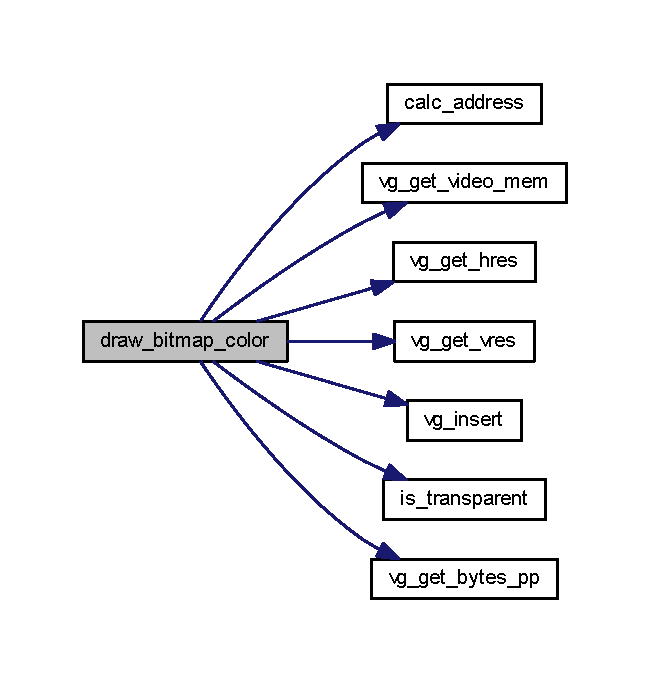
\includegraphics[width=312pt]{group__bitmap_ga0a2714359072f1a1b3f361c89e30be52_cgraph}
\end{center}
\end{figure}
Here is the caller graph for this function\+:\nopagebreak
\begin{figure}[H]
\begin{center}
\leavevmode
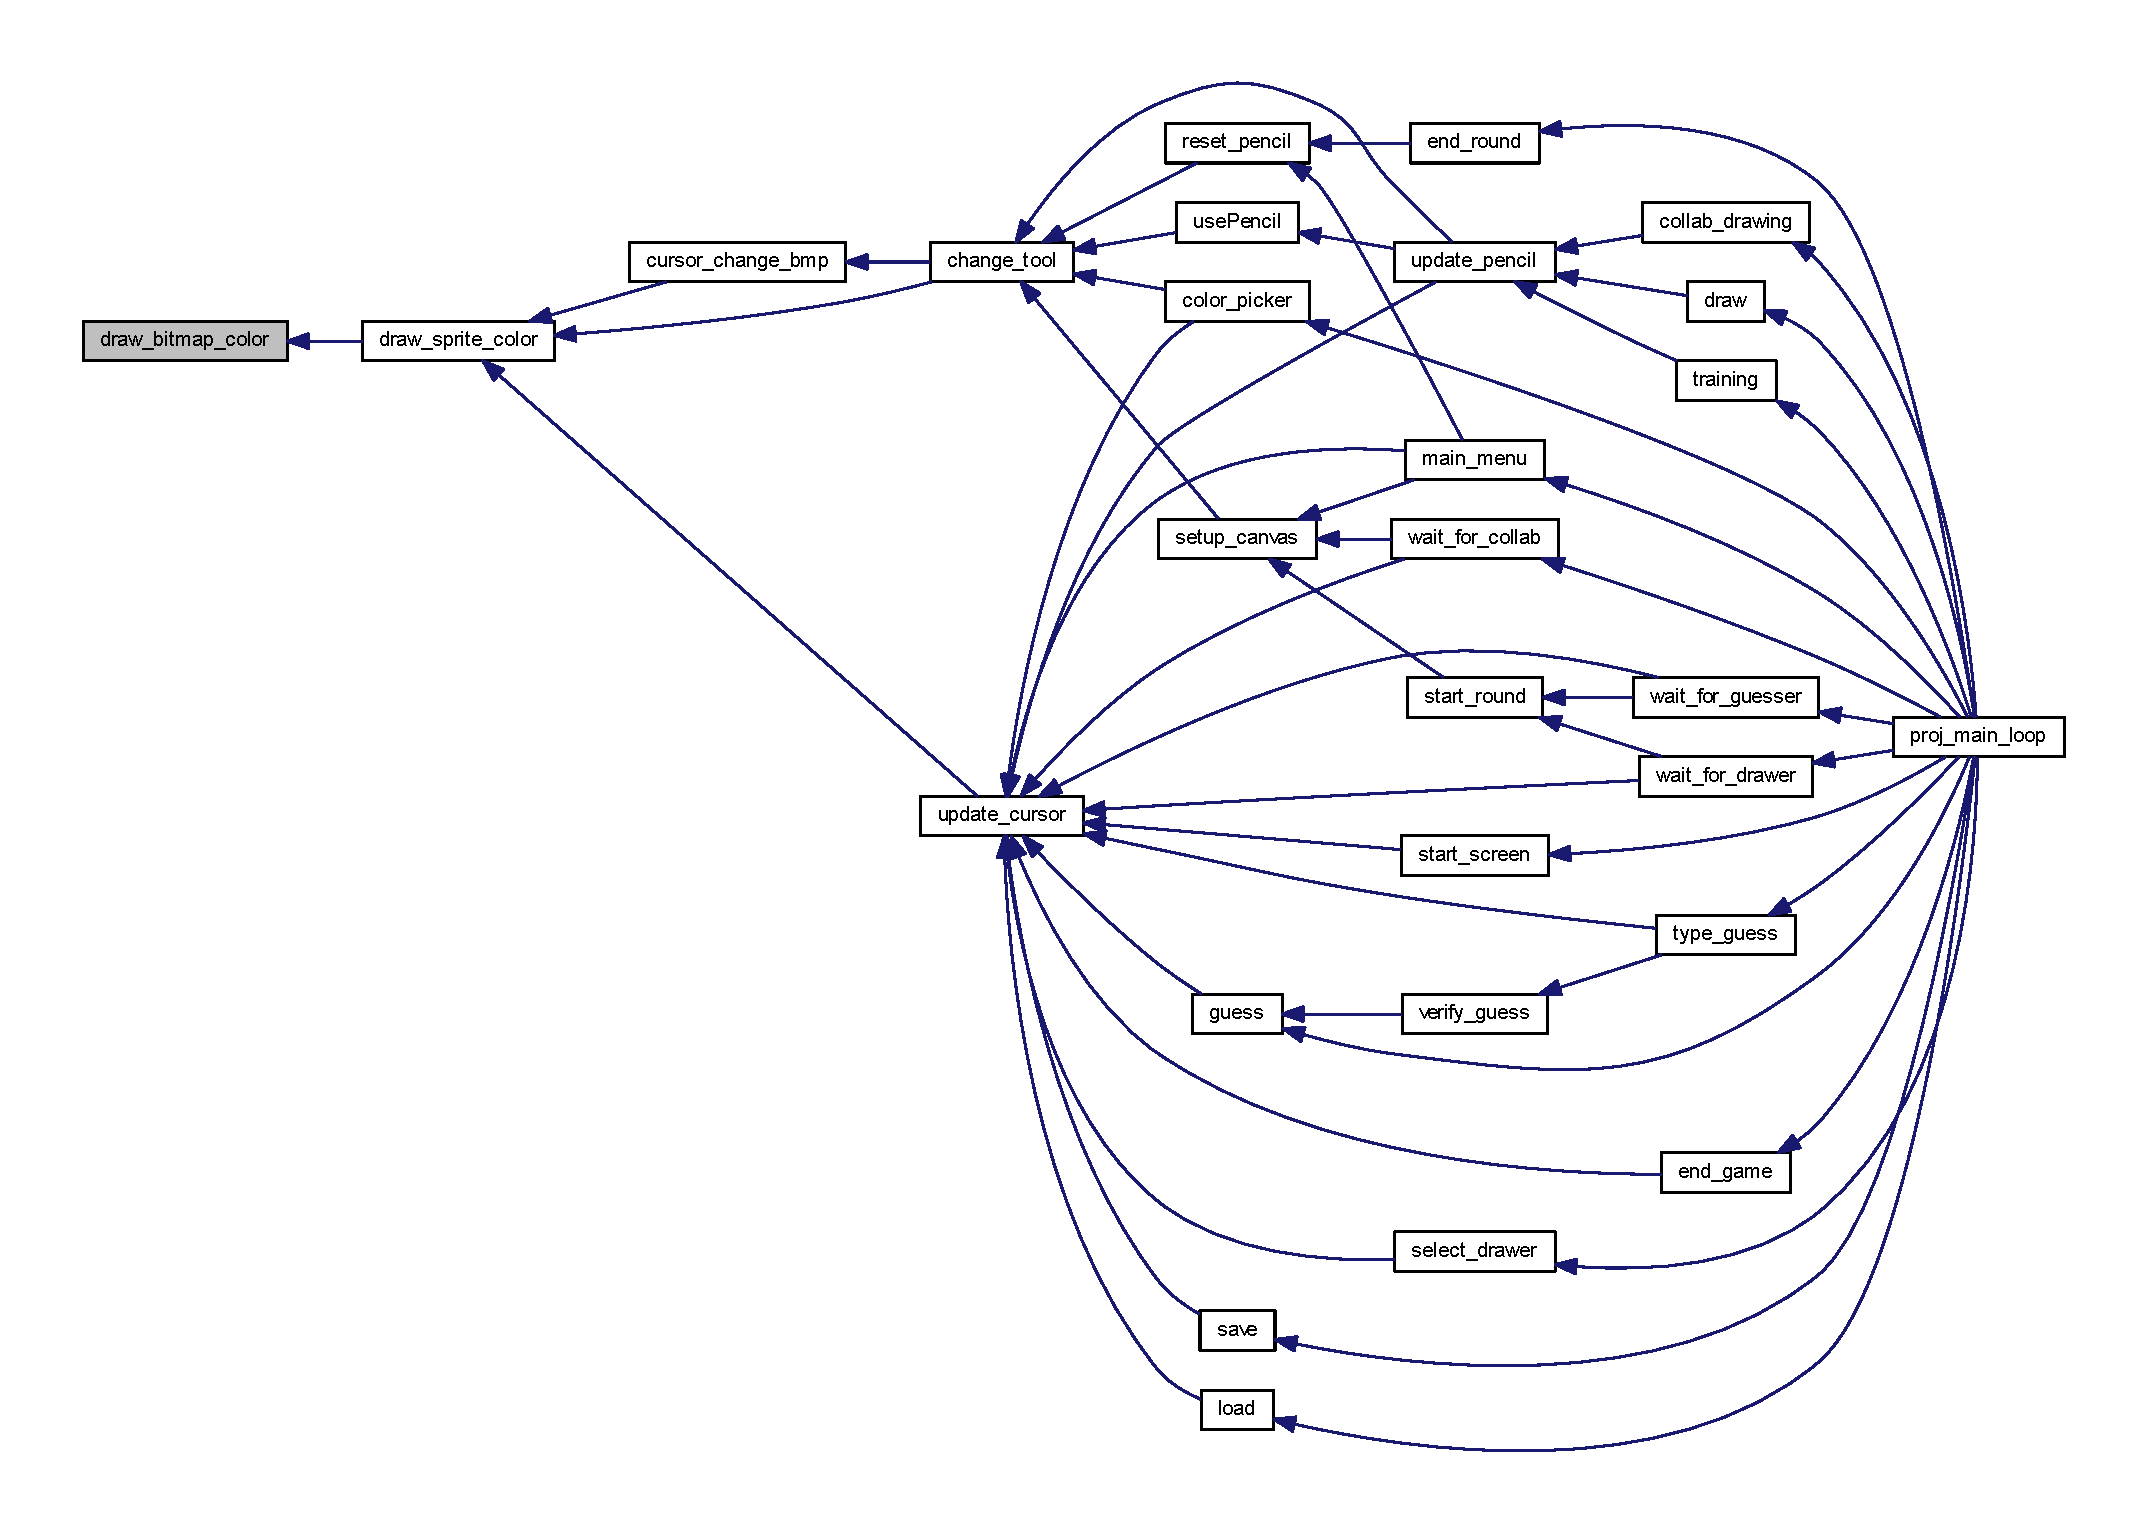
\includegraphics[width=350pt]{group__bitmap_ga0a2714359072f1a1b3f361c89e30be52_icgraph}
\end{center}
\end{figure}
\mbox{\Hypertarget{group__bitmap_ga3c405395b542105657c9811e99c56da4}\label{group__bitmap_ga3c405395b542105657c9811e99c56da4}} 
\index{bitmap@{bitmap}!draw\+\_\+bitmap\+\_\+rotate@{draw\+\_\+bitmap\+\_\+rotate}}
\index{draw\+\_\+bitmap\+\_\+rotate@{draw\+\_\+bitmap\+\_\+rotate}!bitmap@{bitmap}}
\subsubsection{\texorpdfstring{draw\+\_\+bitmap\+\_\+rotate()}{draw\_bitmap\_rotate()}}
{\footnotesize\ttfamily void draw\+\_\+bitmap\+\_\+rotate (\begin{DoxyParamCaption}\item[{\mbox{\hyperlink{struct_bitmap}{Bitmap}} $\ast$}]{bmp,  }\item[{int}]{x,  }\item[{int}]{y,  }\item[{double}]{angle }\end{DoxyParamCaption})}



Draws a bitmap on the screen, rotated by an angle. 


\begin{DoxyParams}{Parameters}
{\em bmp} & Pointer to the \mbox{\hyperlink{struct_bitmap}{Bitmap}} that will be drawn \\
\hline
{\em x} & X position of the upper left corner \\
\hline
{\em y} & Y position of the upper left corner \\
\hline
{\em angle} & Angle rotation \\
\hline
\end{DoxyParams}
Here is the call graph for this function\+:\nopagebreak
\begin{figure}[H]
\begin{center}
\leavevmode
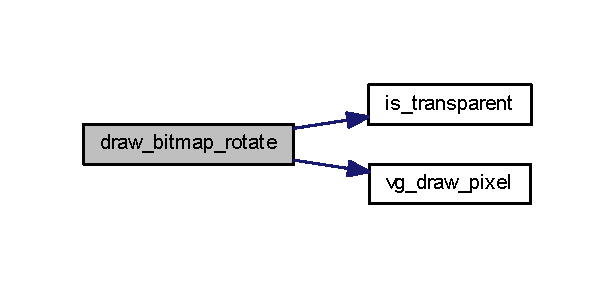
\includegraphics[width=295pt]{group__bitmap_ga3c405395b542105657c9811e99c56da4_cgraph}
\end{center}
\end{figure}
\mbox{\Hypertarget{group__bitmap_ga12d1b6c1fa206ba89cf45d23f6679657}\label{group__bitmap_ga12d1b6c1fa206ba89cf45d23f6679657}} 
\index{bitmap@{bitmap}!draw\+\_\+bitmap\+\_\+transp@{draw\+\_\+bitmap\+\_\+transp}}
\index{draw\+\_\+bitmap\+\_\+transp@{draw\+\_\+bitmap\+\_\+transp}!bitmap@{bitmap}}
\subsubsection{\texorpdfstring{draw\+\_\+bitmap\+\_\+transp()}{draw\_bitmap\_transp()}}
{\footnotesize\ttfamily void draw\+\_\+bitmap\+\_\+transp (\begin{DoxyParamCaption}\item[{\mbox{\hyperlink{struct_bitmap}{Bitmap}} $\ast$}]{bmp,  }\item[{int}]{x,  }\item[{int}]{y,  }\item[{double}]{alpha }\end{DoxyParamCaption})}



Draws a bitmap on the screen, allowing the caller to use transparency. The color B\+L\+A\+CK ignores transparency values. 


\begin{DoxyParams}{Parameters}
{\em bmp} & \mbox{\hyperlink{struct_bitmap}{Bitmap}} to draw \\
\hline
{\em x} & X position of the upper left corner \\
\hline
{\em y} & Y position of the upper left corner \\
\hline
{\em alpha} & Transparency (1 is opaque, 0 is invisible) \\
\hline
\end{DoxyParams}
Here is the call graph for this function\+:\nopagebreak
\begin{figure}[H]
\begin{center}
\leavevmode
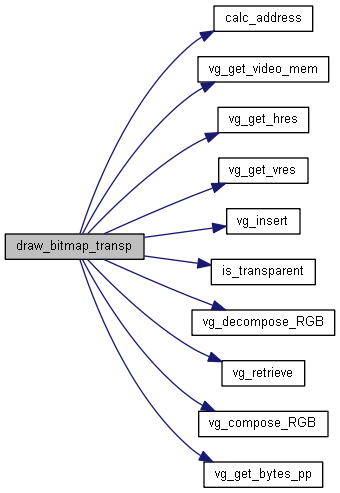
\includegraphics[width=327pt]{group__bitmap_ga12d1b6c1fa206ba89cf45d23f6679657_cgraph}
\end{center}
\end{figure}
Here is the caller graph for this function\+:\nopagebreak
\begin{figure}[H]
\begin{center}
\leavevmode
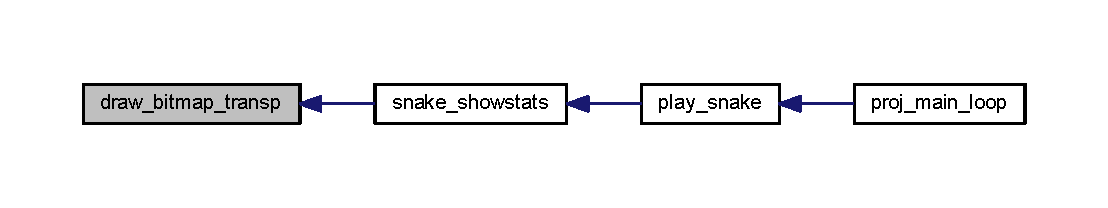
\includegraphics[width=350pt]{group__bitmap_ga12d1b6c1fa206ba89cf45d23f6679657_icgraph}
\end{center}
\end{figure}
\mbox{\Hypertarget{group__bitmap_gad73cdf3b48e5ca2e43ef1fbdd5b061b9}\label{group__bitmap_gad73cdf3b48e5ca2e43ef1fbdd5b061b9}} 
\index{bitmap@{bitmap}!get\+\_\+bitmap\+\_\+color@{get\+\_\+bitmap\+\_\+color}}
\index{get\+\_\+bitmap\+\_\+color@{get\+\_\+bitmap\+\_\+color}!bitmap@{bitmap}}
\subsubsection{\texorpdfstring{get\+\_\+bitmap\+\_\+color()}{get\_bitmap\_color()}}
{\footnotesize\ttfamily uint32\+\_\+t get\+\_\+bitmap\+\_\+color (\begin{DoxyParamCaption}\item[{\mbox{\hyperlink{struct_bitmap}{Bitmap}} $\ast$}]{bmp,  }\item[{uint16\+\_\+t}]{x,  }\item[{uint16\+\_\+t}]{y }\end{DoxyParamCaption})}



Gets the color of a certain bitmap pixel. 


\begin{DoxyParams}{Parameters}
{\em bmp} & Pointer to a \mbox{\hyperlink{struct_bitmap}{Bitmap}} to be read \\
\hline
{\em x} & X position of the pixel, where (0,0) is the upper left corner \\
\hline
{\em y} & Y position of the pixel, where (0,0) is the upper left corner \\
\hline
\end{DoxyParams}
\begin{DoxyReturn}{Returns}
uint32\+\_\+t Respective color 
\end{DoxyReturn}
Here is the caller graph for this function\+:\nopagebreak
\begin{figure}[H]
\begin{center}
\leavevmode
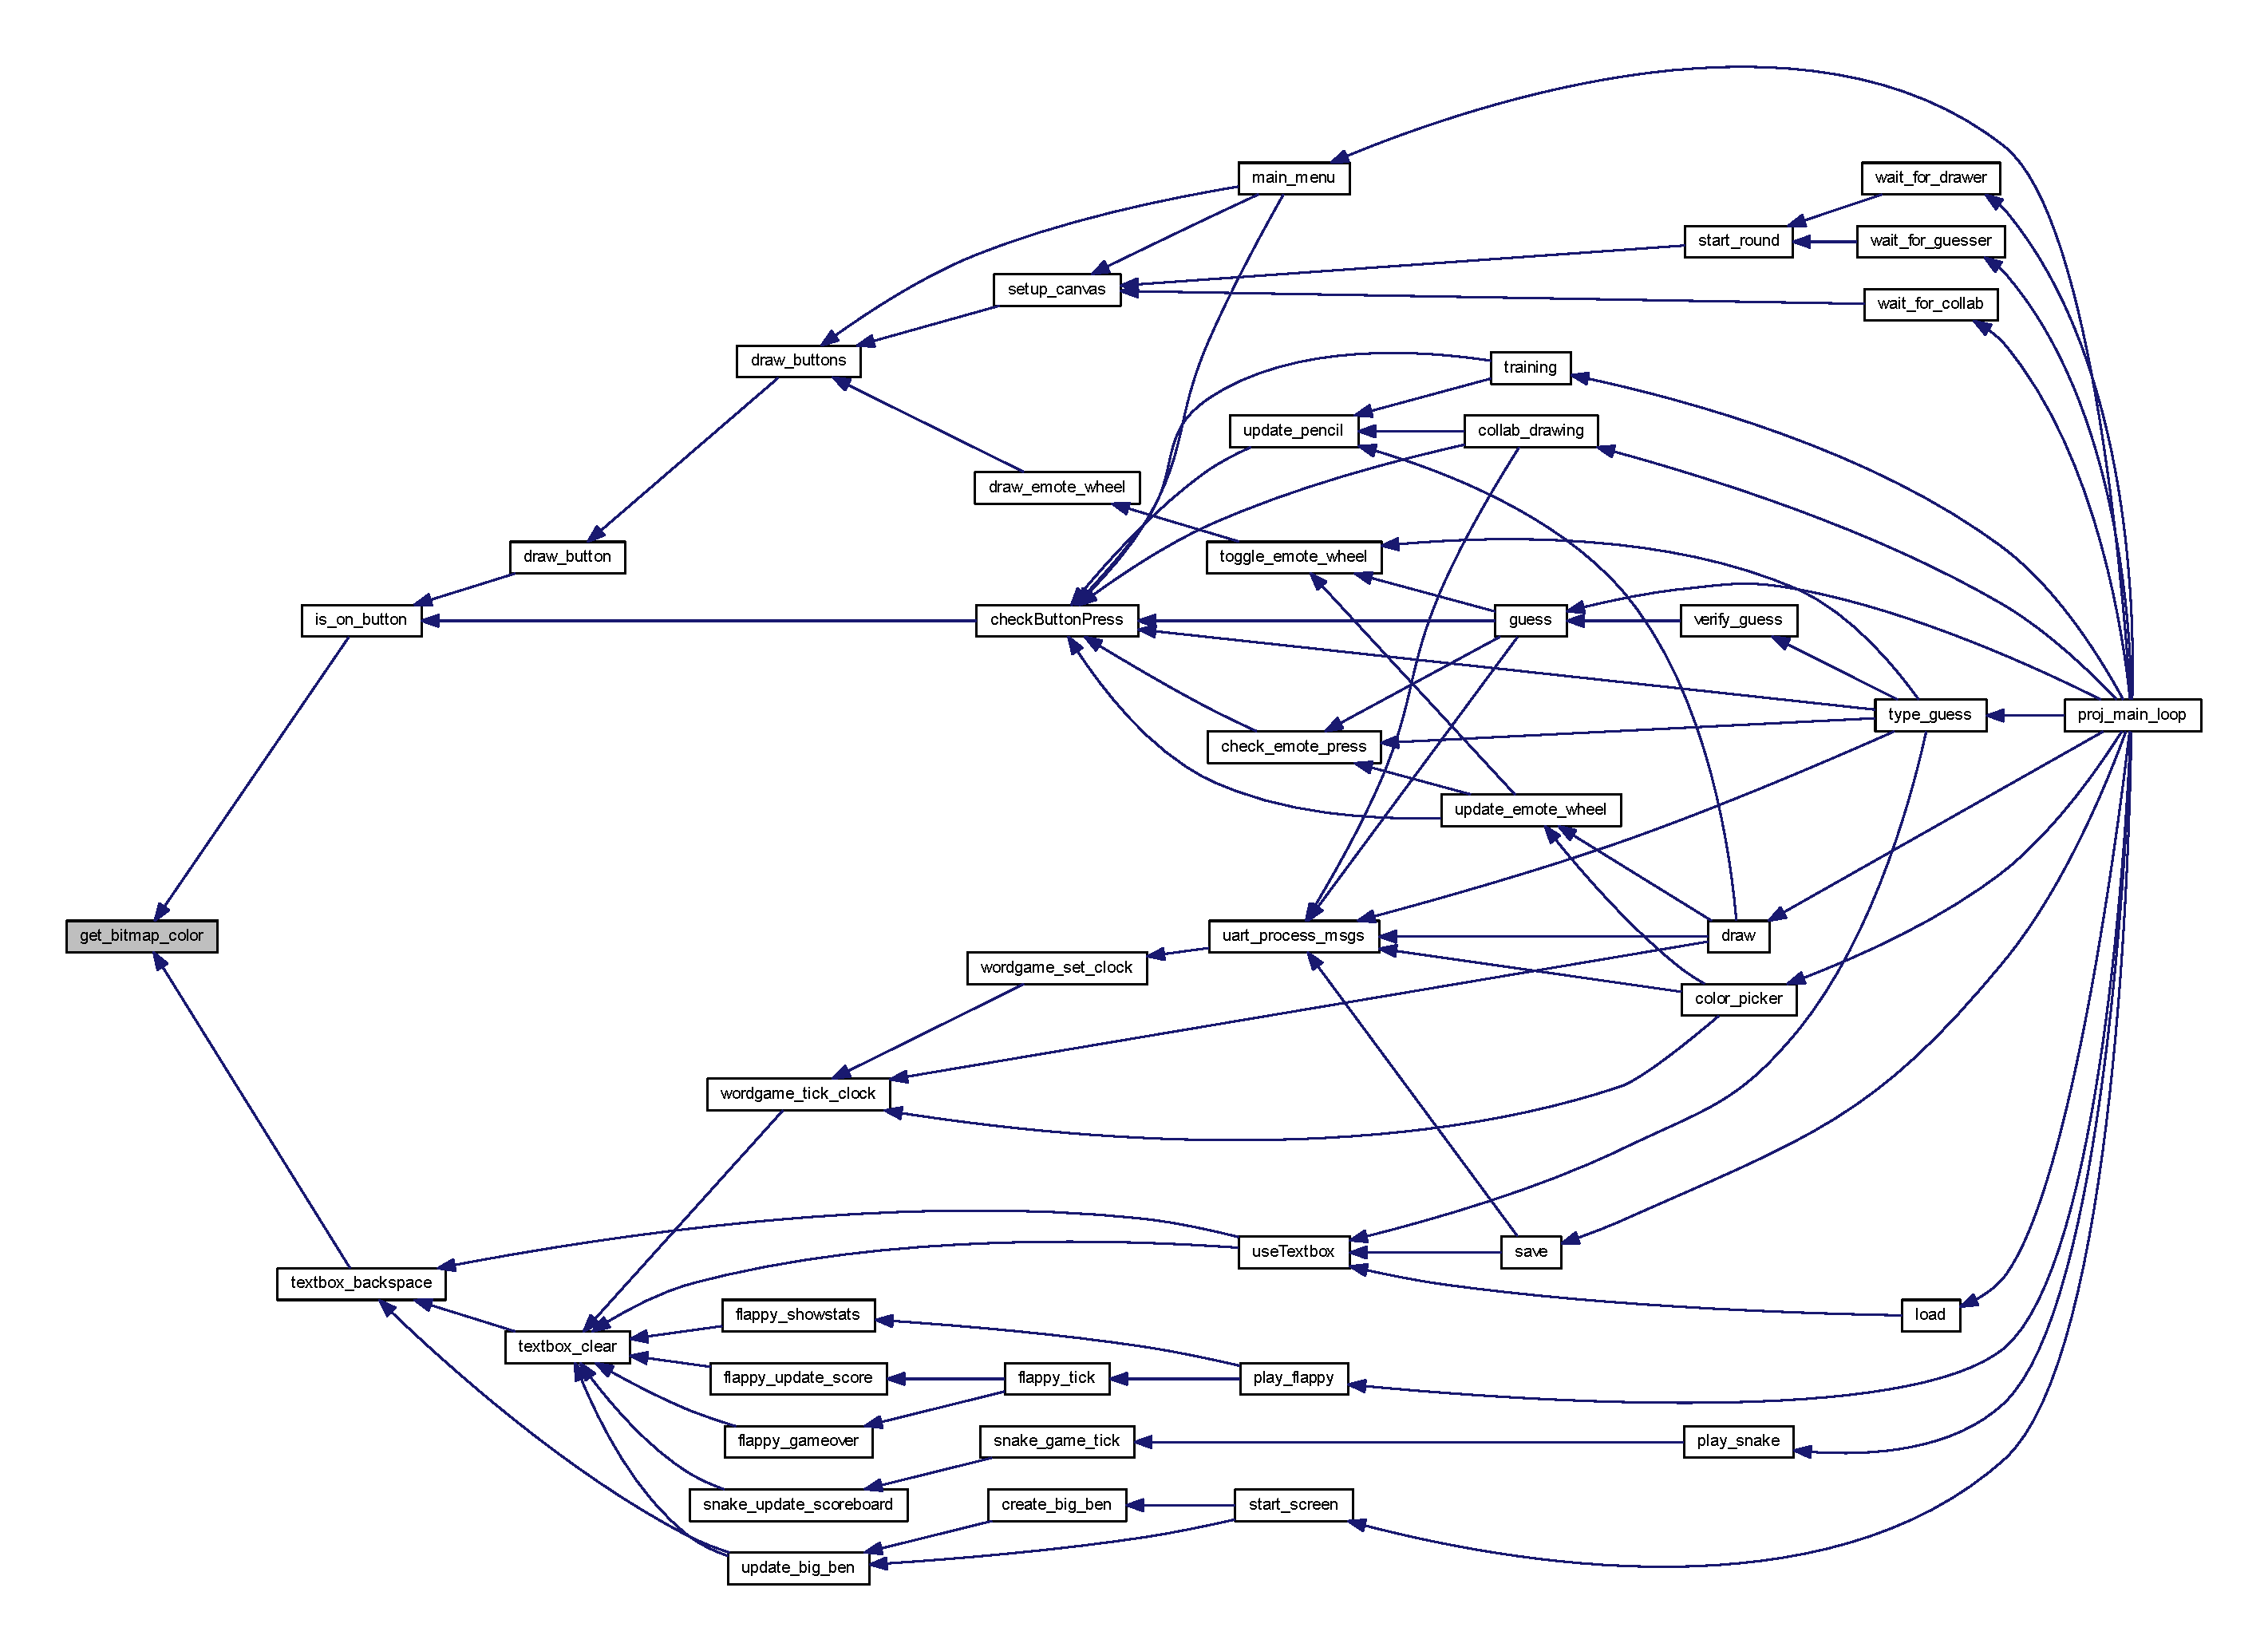
\includegraphics[width=350pt]{group__bitmap_gad73cdf3b48e5ca2e43ef1fbdd5b061b9_icgraph}
\end{center}
\end{figure}
\mbox{\Hypertarget{group__bitmap_ga4b5b3aefecdb54bfdadbe4995b979c7f}\label{group__bitmap_ga4b5b3aefecdb54bfdadbe4995b979c7f}} 
\index{bitmap@{bitmap}!is\+\_\+transparent@{is\+\_\+transparent}}
\index{is\+\_\+transparent@{is\+\_\+transparent}!bitmap@{bitmap}}
\subsubsection{\texorpdfstring{is\+\_\+transparent()}{is\_transparent()}}
{\footnotesize\ttfamily bool is\+\_\+transparent (\begin{DoxyParamCaption}\item[{uint32\+\_\+t}]{color }\end{DoxyParamCaption})}



Checks if a color is transparent (M\+A\+G\+E\+N\+TA) 


\begin{DoxyParams}{Parameters}
{\em color} & Color to compare \\
\hline
\end{DoxyParams}
\begin{DoxyReturn}{Returns}
true The color is transparent (M\+A\+G\+E\+N\+TA) 

false The color is transparent (M\+A\+G\+E\+N\+TA) 
\end{DoxyReturn}
Here is the caller graph for this function\+:\nopagebreak
\begin{figure}[H]
\begin{center}
\leavevmode
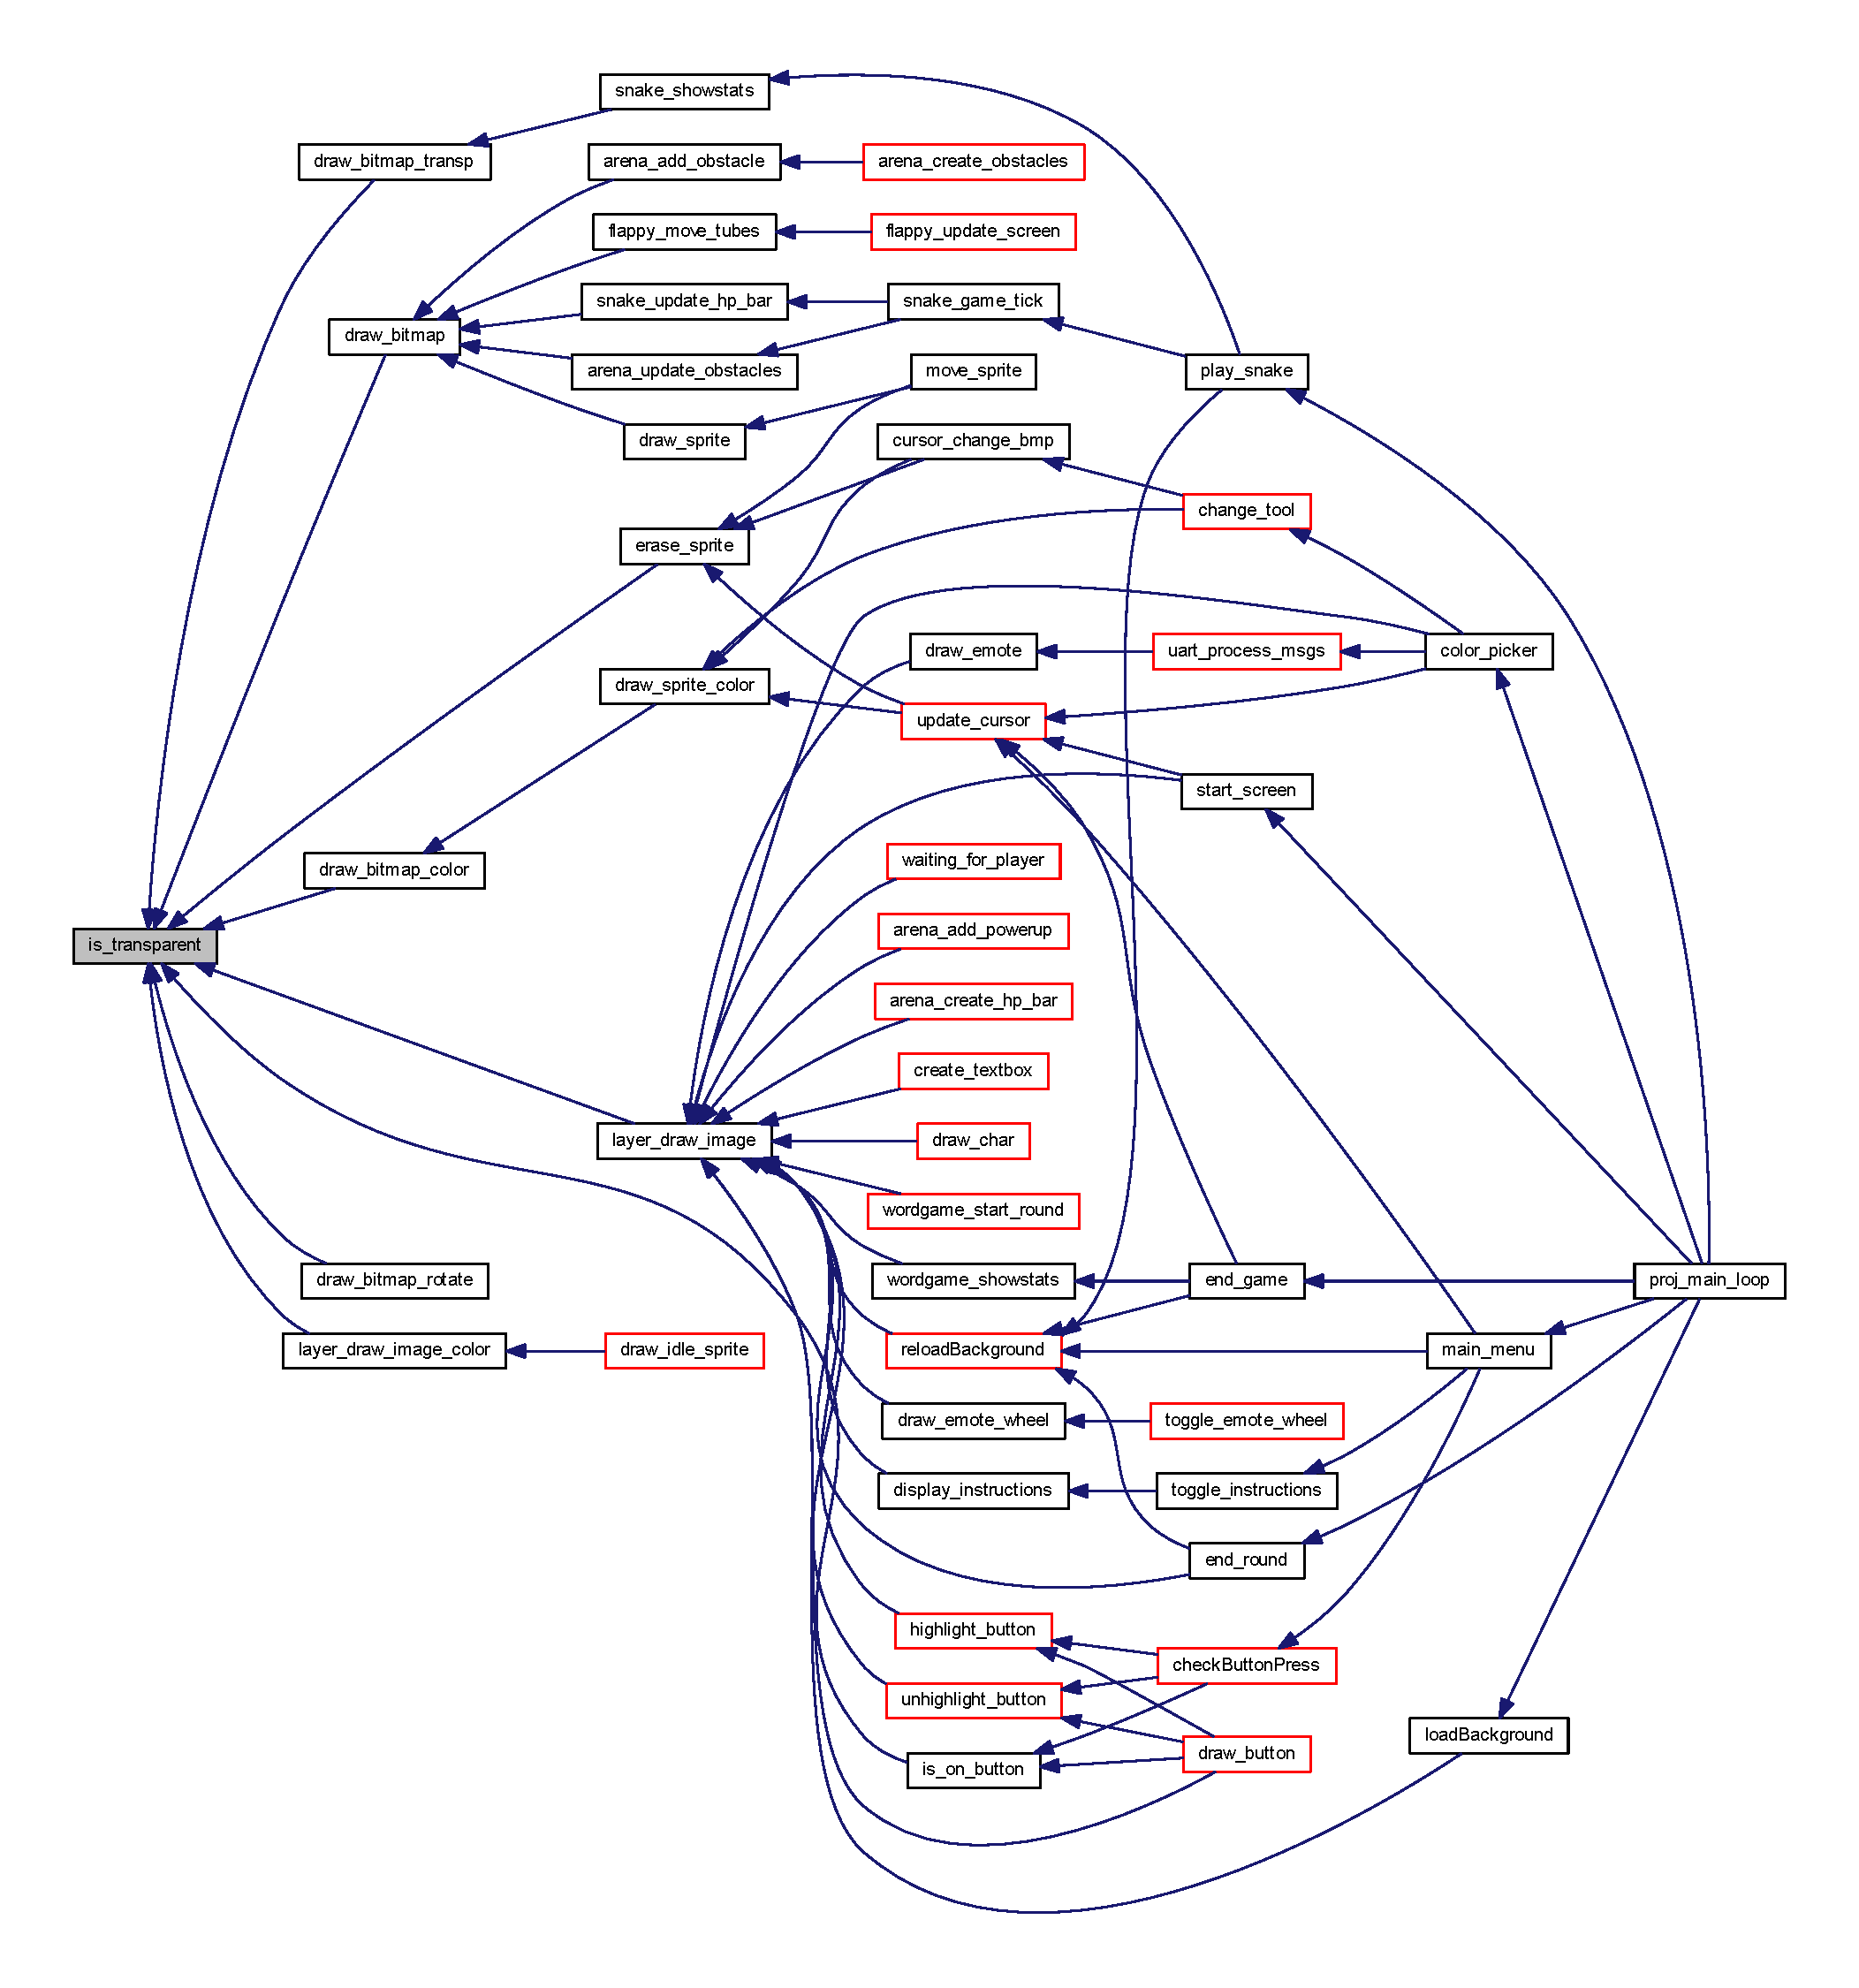
\includegraphics[width=350pt]{group__bitmap_ga4b5b3aefecdb54bfdadbe4995b979c7f_icgraph}
\end{center}
\end{figure}
\mbox{\Hypertarget{group__bitmap_ga627d64d58e9bf487fb6e326ea65df57b}\label{group__bitmap_ga627d64d58e9bf487fb6e326ea65df57b}} 
\index{bitmap@{bitmap}!load\+Bitmap@{load\+Bitmap}}
\index{load\+Bitmap@{load\+Bitmap}!bitmap@{bitmap}}
\subsubsection{\texorpdfstring{load\+Bitmap()}{loadBitmap()}}
{\footnotesize\ttfamily \mbox{\hyperlink{struct_bitmap}{Bitmap}}$\ast$ load\+Bitmap (\begin{DoxyParamCaption}\item[{const char $\ast$}]{folder\+Path,  }\item[{const char $\ast$}]{filename }\end{DoxyParamCaption})}



Loads a .bmp file. 


\begin{DoxyParams}{Parameters}
{\em folder\+Path} & Full folder path. \\
\hline
{\em filename} & File name, including .bmp \\
\hline
\end{DoxyParams}
\begin{DoxyReturn}{Returns}
Bitmap$\ast$ Pointer to the respective bitmap structure 
\end{DoxyReturn}
Here is the caller graph for this function\+:\nopagebreak
\begin{figure}[H]
\begin{center}
\leavevmode
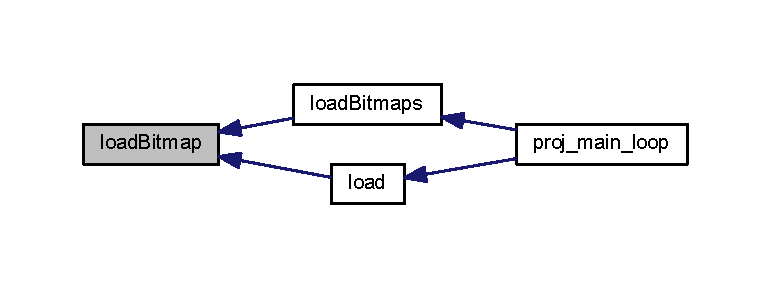
\includegraphics[width=350pt]{group__bitmap_ga627d64d58e9bf487fb6e326ea65df57b_icgraph}
\end{center}
\end{figure}
\mbox{\Hypertarget{group__bitmap_ga3f8f5ad40944f2db40792d7c4fe5b96e}\label{group__bitmap_ga3f8f5ad40944f2db40792d7c4fe5b96e}} 
\index{bitmap@{bitmap}!load\+Bitmap\+Section@{load\+Bitmap\+Section}}
\index{load\+Bitmap\+Section@{load\+Bitmap\+Section}!bitmap@{bitmap}}
\subsubsection{\texorpdfstring{load\+Bitmap\+Section()}{loadBitmapSection()}}
{\footnotesize\ttfamily \mbox{\hyperlink{struct_bitmap}{Bitmap}}$\ast$ load\+Bitmap\+Section (\begin{DoxyParamCaption}\item[{\mbox{\hyperlink{struct_bitmap}{Bitmap}} $\ast$}]{bitmap,  }\item[{uint16\+\_\+t}]{x,  }\item[{uint16\+\_\+t}]{y,  }\item[{uint16\+\_\+t}]{width,  }\item[{uint16\+\_\+t}]{height }\end{DoxyParamCaption})}



Copies part of a bitmap from a given bitmap to another bitmap. 


\begin{DoxyParams}{Parameters}
{\em bitmap} & \char`\"{}\+Bigger\char`\"{} bitmap to read \\
\hline
{\em x} & X position to start copying the contents from \\
\hline
{\em y} & Y position to start copying the contents from \\
\hline
{\em width} & Width of the area to copy \\
\hline
{\em height} & Height of the area to copy \\
\hline
\end{DoxyParams}
\begin{DoxyReturn}{Returns}
Bitmap$\ast$ Returns a pointer to the cropped bitmap 
\end{DoxyReturn}
Here is the caller graph for this function\+:\nopagebreak
\begin{figure}[H]
\begin{center}
\leavevmode
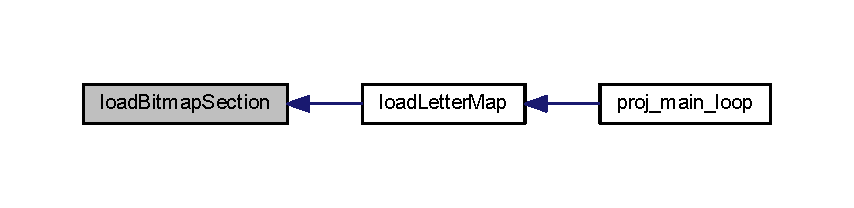
\includegraphics[width=350pt]{group__bitmap_ga3f8f5ad40944f2db40792d7c4fe5b96e_icgraph}
\end{center}
\end{figure}
\mbox{\Hypertarget{group__bitmap_gaa19cec779e8cbaf053f3efc749c20c37}\label{group__bitmap_gaa19cec779e8cbaf053f3efc749c20c37}} 
\index{bitmap@{bitmap}!resize\+Bitmap@{resize\+Bitmap}}
\index{resize\+Bitmap@{resize\+Bitmap}!bitmap@{bitmap}}
\subsubsection{\texorpdfstring{resize\+Bitmap()}{resizeBitmap()}}
{\footnotesize\ttfamily \mbox{\hyperlink{struct_bitmap}{Bitmap}}$\ast$ resize\+Bitmap (\begin{DoxyParamCaption}\item[{\mbox{\hyperlink{struct_bitmap}{Bitmap}} $\ast$}]{bitmap,  }\item[{uint16\+\_\+t}]{factor }\end{DoxyParamCaption})}



Resizes a bitmap by a given factor. 


\begin{DoxyParams}{Parameters}
{\em bitmap} & \mbox{\hyperlink{struct_bitmap}{Bitmap}} to resize \\
\hline
{\em factor} & Factor (Must be an integer \+:( ) \\
\hline
\end{DoxyParams}
\begin{DoxyReturn}{Returns}
Bitmap$\ast$ Returns a pointer to the resized bitmap 
\end{DoxyReturn}
Here is the caller graph for this function\+:\nopagebreak
\begin{figure}[H]
\begin{center}
\leavevmode
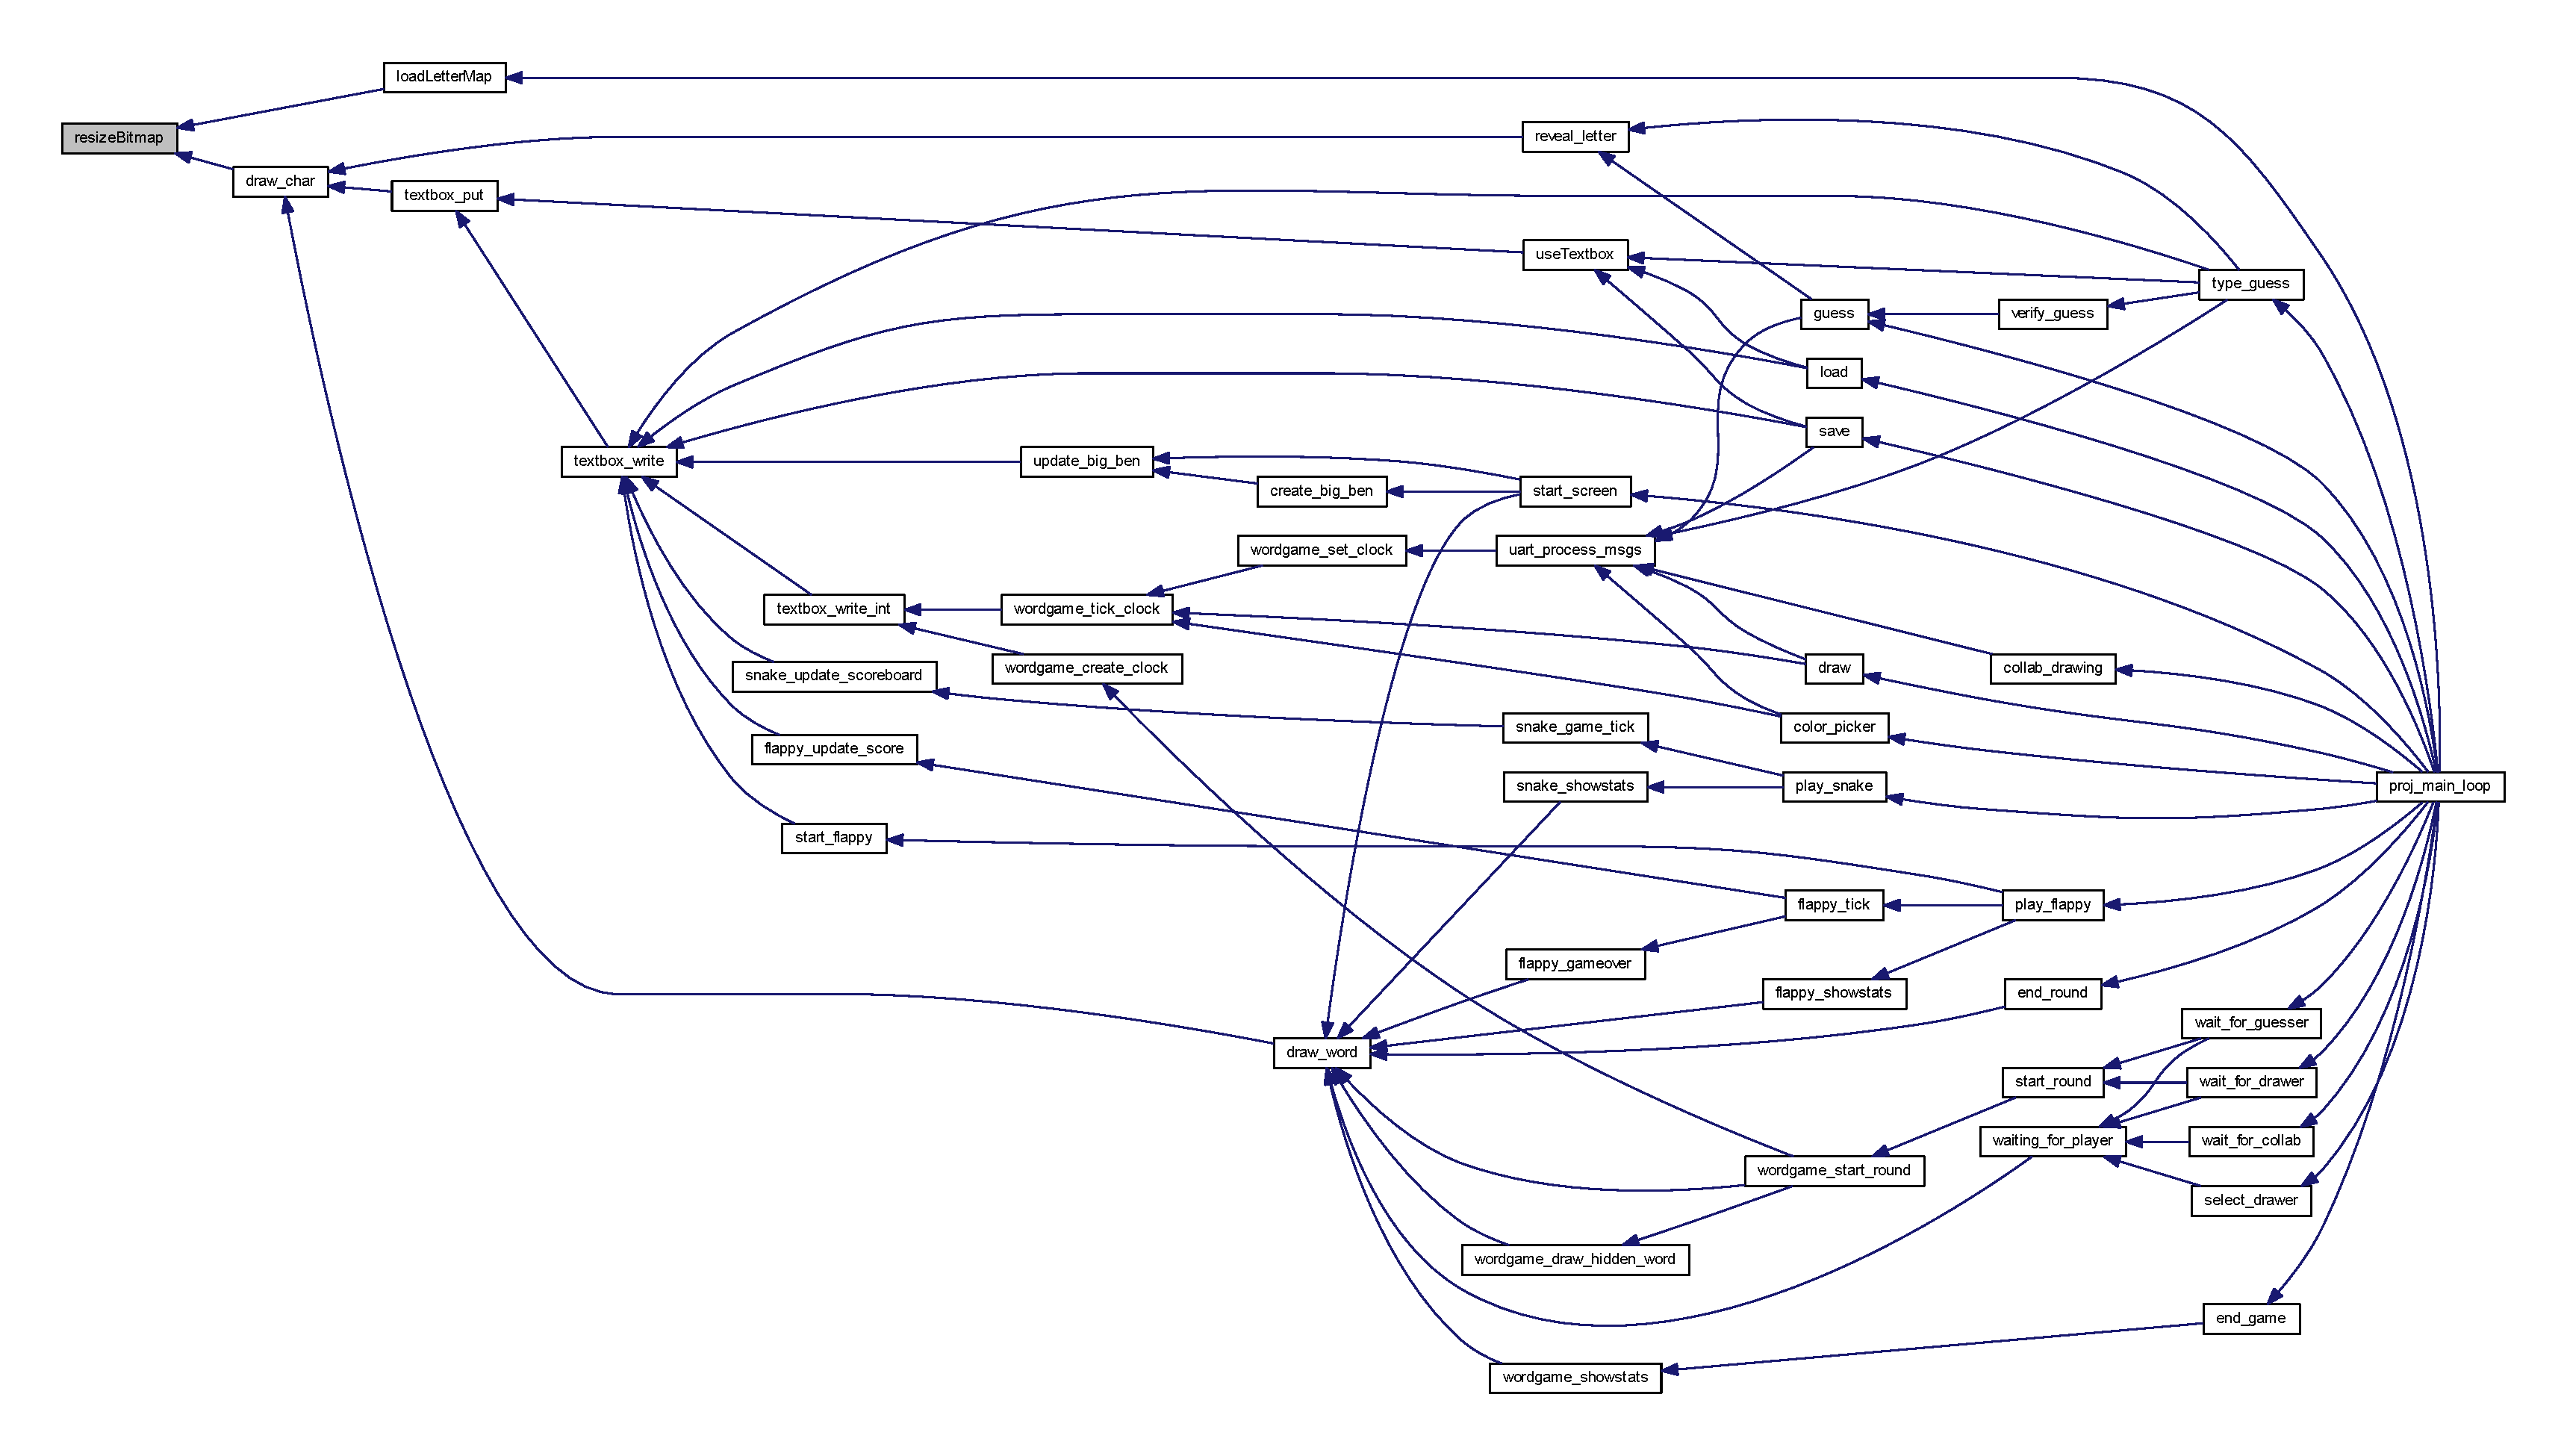
\includegraphics[width=350pt]{group__bitmap_gaa19cec779e8cbaf053f3efc749c20c37_icgraph}
\end{center}
\end{figure}
\mbox{\Hypertarget{group__bitmap_gacc8595ed81c710cecebe95f04db413fe}\label{group__bitmap_gacc8595ed81c710cecebe95f04db413fe}} 
\index{bitmap@{bitmap}!save\+Bitmap@{save\+Bitmap}}
\index{save\+Bitmap@{save\+Bitmap}!bitmap@{bitmap}}
\subsubsection{\texorpdfstring{save\+Bitmap()}{saveBitmap()}}
{\footnotesize\ttfamily void save\+Bitmap (\begin{DoxyParamCaption}\item[{char $\ast$}]{path,  }\item[{unsigned int}]{width,  }\item[{unsigned int}]{height,  }\item[{char $\ast$}]{address }\end{DoxyParamCaption})}



Saves a bitmap in a .bmp file. 


\begin{DoxyParams}{Parameters}
{\em path} & Full path of the saved file. \\
\hline
{\em width} & \mbox{\hyperlink{struct_bitmap}{Bitmap}} width, in pixels \\
\hline
{\em height} & \mbox{\hyperlink{struct_bitmap}{Bitmap}} height, in pixels \\
\hline
{\em address} & Pointer to a pixel map. \\
\hline
\end{DoxyParams}
Here is the call graph for this function\+:\nopagebreak
\begin{figure}[H]
\begin{center}
\leavevmode
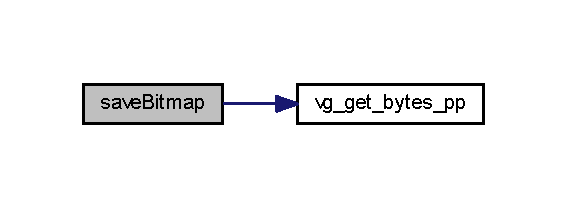
\includegraphics[width=272pt]{group__bitmap_gacc8595ed81c710cecebe95f04db413fe_cgraph}
\end{center}
\end{figure}
Here is the caller graph for this function\+:\nopagebreak
\begin{figure}[H]
\begin{center}
\leavevmode
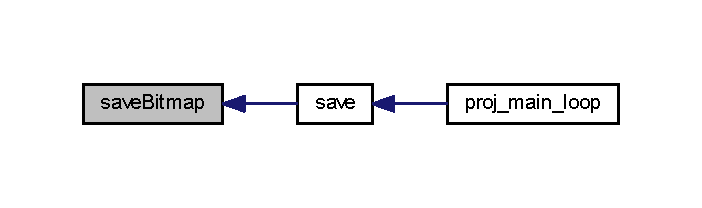
\includegraphics[width=337pt]{group__bitmap_gacc8595ed81c710cecebe95f04db413fe_icgraph}
\end{center}
\end{figure}


\subsection{Variable Documentation}
\mbox{\Hypertarget{group__bitmap_ga65e6af125468dec1b3b7cf18fad3800f}\label{group__bitmap_ga65e6af125468dec1b3b7cf18fad3800f}} 
\index{bitmap@{bitmap}!actual\+\_\+bytes\+\_\+per\+\_\+row@{actual\+\_\+bytes\+\_\+per\+\_\+row}}
\index{actual\+\_\+bytes\+\_\+per\+\_\+row@{actual\+\_\+bytes\+\_\+per\+\_\+row}!bitmap@{bitmap}}
\subsubsection{\texorpdfstring{actual\+\_\+bytes\+\_\+per\+\_\+row}{actual\_bytes\_per\_row}}
{\footnotesize\ttfamily unsigned int Bitmap\+::actual\+\_\+bytes\+\_\+per\+\_\+row}



Number of bytes per row (including padding) 

\mbox{\Hypertarget{group__bitmap_gad3fa2b9ac8c411719d9c261f41a999f9}\label{group__bitmap_gad3fa2b9ac8c411719d9c261f41a999f9}} 
\index{bitmap@{bitmap}!bitmap\+Data@{bitmap\+Data}}
\index{bitmap\+Data@{bitmap\+Data}!bitmap@{bitmap}}
\subsubsection{\texorpdfstring{bitmap\+Data}{bitmapData}}
{\footnotesize\ttfamily char$\ast$ Bitmap\+::bitmap\+Data}



Pointer to the pixel map buffer. 

\mbox{\Hypertarget{group__bitmap_ga95c481a5ce1ff4af08cd135ca4af120b}\label{group__bitmap_ga95c481a5ce1ff4af08cd135ca4af120b}} 
\index{bitmap@{bitmap}!bitmap\+Info\+Header@{bitmap\+Info\+Header}}
\index{bitmap\+Info\+Header@{bitmap\+Info\+Header}!bitmap@{bitmap}}
\subsubsection{\texorpdfstring{bitmap\+Info\+Header}{bitmapInfoHeader}}
{\footnotesize\ttfamily \mbox{\hyperlink{struct_bitmap_info_header}{Bitmap\+Info\+Header}} Bitmap\+::bitmap\+Info\+Header}



\mbox{\hyperlink{struct_bitmap}{Bitmap}} info header. 

\mbox{\Hypertarget{group__bitmap_ga2a1eb136325c8cb16aeeb7108703702f}\label{group__bitmap_ga2a1eb136325c8cb16aeeb7108703702f}} 
\index{bitmap@{bitmap}!bits\+Per\+Pixel@{bits\+Per\+Pixel}}
\index{bits\+Per\+Pixel@{bits\+Per\+Pixel}!bitmap@{bitmap}}
\subsubsection{\texorpdfstring{bits\+Per\+Pixel}{bitsPerPixel}}
{\footnotesize\ttfamily unsigned short Bitmap\+Info\+Header\+::bits\+Per\+Pixel}



specifies the number of bit per pixel 

\mbox{\Hypertarget{group__bitmap_gac4487f25d79f268d5bb0580e68e82b53}\label{group__bitmap_gac4487f25d79f268d5bb0580e68e82b53}} 
\index{bitmap@{bitmap}!bytes\+\_\+per\+\_\+pixel@{bytes\+\_\+per\+\_\+pixel}}
\index{bytes\+\_\+per\+\_\+pixel@{bytes\+\_\+per\+\_\+pixel}!bitmap@{bitmap}}
\subsubsection{\texorpdfstring{bytes\+\_\+per\+\_\+pixel}{bytes\_per\_pixel}}
{\footnotesize\ttfamily unsigned int Bitmap\+::bytes\+\_\+per\+\_\+pixel}



Bytes per pixel used by the bitmap. 

\mbox{\Hypertarget{group__bitmap_ga87fb38b0fe68db4bed899b9733d1b7e9}\label{group__bitmap_ga87fb38b0fe68db4bed899b9733d1b7e9}} 
\index{bitmap@{bitmap}!compression@{compression}}
\index{compression@{compression}!bitmap@{bitmap}}
\subsubsection{\texorpdfstring{compression}{compression}}
{\footnotesize\ttfamily unsigned int Bitmap\+Info\+Header\+::compression}



specifies the type of compression 

\mbox{\Hypertarget{group__bitmap_gaaa1d31efc13210020a38d435e4961df9}\label{group__bitmap_gaaa1d31efc13210020a38d435e4961df9}} 
\index{bitmap@{bitmap}!height@{height}}
\index{height@{height}!bitmap@{bitmap}}
\subsubsection{\texorpdfstring{height}{height}}
{\footnotesize\ttfamily int Bitmap\+Info\+Header\+::height}



specifies height in pixels 

\mbox{\Hypertarget{group__bitmap_ga79bc984a7fd1c0f00ede6aa09143939f}\label{group__bitmap_ga79bc984a7fd1c0f00ede6aa09143939f}} 
\index{bitmap@{bitmap}!image\+Size@{image\+Size}}
\index{image\+Size@{image\+Size}!bitmap@{bitmap}}
\subsubsection{\texorpdfstring{image\+Size}{imageSize}}
{\footnotesize\ttfamily unsigned int Bitmap\+Info\+Header\+::image\+Size}



size of image in bytes 

\mbox{\Hypertarget{group__bitmap_ga9d87941fcc414085f7361fd89818ee3f}\label{group__bitmap_ga9d87941fcc414085f7361fd89818ee3f}} 
\index{bitmap@{bitmap}!important\+Colors@{important\+Colors}}
\index{important\+Colors@{important\+Colors}!bitmap@{bitmap}}
\subsubsection{\texorpdfstring{important\+Colors}{importantColors}}
{\footnotesize\ttfamily unsigned int Bitmap\+Info\+Header\+::important\+Colors}



number of colors that are important 

\mbox{\Hypertarget{group__bitmap_ga4c543a08d1b72bdda2329b426a213e2a}\label{group__bitmap_ga4c543a08d1b72bdda2329b426a213e2a}} 
\index{bitmap@{bitmap}!n\+Colors@{n\+Colors}}
\index{n\+Colors@{n\+Colors}!bitmap@{bitmap}}
\subsubsection{\texorpdfstring{n\+Colors}{nColors}}
{\footnotesize\ttfamily unsigned int Bitmap\+Info\+Header\+::n\+Colors}



number of colors used by the bitmap 

\mbox{\Hypertarget{group__bitmap_ga26ed598693b100ffd9e29c4dc77f3d92}\label{group__bitmap_ga26ed598693b100ffd9e29c4dc77f3d92}} 
\index{bitmap@{bitmap}!offset@{offset}}
\index{offset@{offset}!bitmap@{bitmap}}
\subsubsection{\texorpdfstring{offset}{offset}}
{\footnotesize\ttfamily unsigned int Bitmap\+File\+Header\+::offset}



specifies the offset in bytes from the bitmapfileheader to the bitmap bits 

\mbox{\Hypertarget{group__bitmap_ga0ff33a06b37b2b310a499b4ef19fb490}\label{group__bitmap_ga0ff33a06b37b2b310a499b4ef19fb490}} 
\index{bitmap@{bitmap}!padding@{padding}}
\index{padding@{padding}!bitmap@{bitmap}}
\subsubsection{\texorpdfstring{padding}{padding}}
{\footnotesize\ttfamily unsigned int Bitmap\+::padding}



\mbox{\hyperlink{struct_bitmap}{Bitmap}} padding per row. 

\mbox{\Hypertarget{group__bitmap_ga9925e97e8bbc6b797afe2d22fbab45d6}\label{group__bitmap_ga9925e97e8bbc6b797afe2d22fbab45d6}} 
\index{bitmap@{bitmap}!planes@{planes}}
\index{planes@{planes}!bitmap@{bitmap}}
\subsubsection{\texorpdfstring{planes}{planes}}
{\footnotesize\ttfamily unsigned short Bitmap\+Info\+Header\+::planes}



specifies the number of color planes, must be 1 

\mbox{\Hypertarget{group__bitmap_ga16d8cfe2edb9d109cea44ab94d1b701a}\label{group__bitmap_ga16d8cfe2edb9d109cea44ab94d1b701a}} 
\index{bitmap@{bitmap}!reserved1@{reserved1}}
\index{reserved1@{reserved1}!bitmap@{bitmap}}
\subsubsection{\texorpdfstring{reserved1}{reserved1}}
{\footnotesize\ttfamily unsigned short Bitmap\+File\+Header\+::reserved1}



reserved; must be 0 

\mbox{\Hypertarget{group__bitmap_ga24130729dee5b8b9c1bd45f0a73c9a9d}\label{group__bitmap_ga24130729dee5b8b9c1bd45f0a73c9a9d}} 
\index{bitmap@{bitmap}!reserved2@{reserved2}}
\index{reserved2@{reserved2}!bitmap@{bitmap}}
\subsubsection{\texorpdfstring{reserved2}{reserved2}}
{\footnotesize\ttfamily unsigned short int Bitmap\+File\+Header\+::reserved2}



reserved; must be 0 

\mbox{\Hypertarget{group__bitmap_ga0dcad71d9b17783c4d296c2c6d00ede0}\label{group__bitmap_ga0dcad71d9b17783c4d296c2c6d00ede0}} 
\index{bitmap@{bitmap}!size@{size}}
\index{size@{size}!bitmap@{bitmap}}
\subsubsection{\texorpdfstring{size}{size}\hspace{0.1cm}{\footnotesize\ttfamily [1/2]}}
{\footnotesize\ttfamily unsigned int Bitmap\+File\+Header\+::size}



specifies the size in bytes of the bitmap file 

\mbox{\Hypertarget{group__bitmap_ga411fa70f6547a0360b33edcd3273d169}\label{group__bitmap_ga411fa70f6547a0360b33edcd3273d169}} 
\index{bitmap@{bitmap}!size@{size}}
\index{size@{size}!bitmap@{bitmap}}
\subsubsection{\texorpdfstring{size}{size}\hspace{0.1cm}{\footnotesize\ttfamily [2/2]}}
{\footnotesize\ttfamily unsigned int Bitmap\+Info\+Header\+::size}



specifies the number of bytes required by the struct 

\mbox{\Hypertarget{group__bitmap_ga0206e64e29930b0594e714cbdf8090f0}\label{group__bitmap_ga0206e64e29930b0594e714cbdf8090f0}} 
\index{bitmap@{bitmap}!type@{type}}
\index{type@{type}!bitmap@{bitmap}}
\subsubsection{\texorpdfstring{type}{type}}
{\footnotesize\ttfamily unsigned short int Bitmap\+File\+Header\+::type}



specifies the file type 

\mbox{\Hypertarget{group__bitmap_gac2034cfbada460819beed1ee24581c5d}\label{group__bitmap_gac2034cfbada460819beed1ee24581c5d}} 
\index{bitmap@{bitmap}!width@{width}}
\index{width@{width}!bitmap@{bitmap}}
\subsubsection{\texorpdfstring{width}{width}}
{\footnotesize\ttfamily int Bitmap\+Info\+Header\+::width}



specifies width in pixels 

\mbox{\Hypertarget{group__bitmap_ga391cf1da75d16aee3b6539ccf5b29300}\label{group__bitmap_ga391cf1da75d16aee3b6539ccf5b29300}} 
\index{bitmap@{bitmap}!x\+Resolution@{x\+Resolution}}
\index{x\+Resolution@{x\+Resolution}!bitmap@{bitmap}}
\subsubsection{\texorpdfstring{x\+Resolution}{xResolution}}
{\footnotesize\ttfamily int Bitmap\+Info\+Header\+::x\+Resolution}



number of pixels per meter in x axis 

\mbox{\Hypertarget{group__bitmap_gaf2fadf9c216cc9f3ce401096e35be1b7}\label{group__bitmap_gaf2fadf9c216cc9f3ce401096e35be1b7}} 
\index{bitmap@{bitmap}!y\+Resolution@{y\+Resolution}}
\index{y\+Resolution@{y\+Resolution}!bitmap@{bitmap}}
\subsubsection{\texorpdfstring{y\+Resolution}{yResolution}}
{\footnotesize\ttfamily int Bitmap\+Info\+Header\+::y\+Resolution}



number of pixels per meter in y axis 


\hypertarget{group__bitmaps}{}\section{bitmaps}
\label{group__bitmaps}\index{bitmaps@{bitmaps}}
\subsection*{Functions}
\begin{DoxyCompactItemize}
\item 
void \mbox{\hyperlink{group__bitmaps_ga5a66eb06403c650e88bc9463e79bf9bc}{load\+Bitmaps}} (const char $\ast$folder\+Path)
\begin{DoxyCompactList}\small\item\em Looks for specific .bmp files in a folder and loads them. \end{DoxyCompactList}\end{DoxyCompactItemize}


\subsection{Detailed Description}
Functions used load bitmaps 

\subsection{Function Documentation}
\mbox{\Hypertarget{group__bitmaps_ga5a66eb06403c650e88bc9463e79bf9bc}\label{group__bitmaps_ga5a66eb06403c650e88bc9463e79bf9bc}} 
\index{bitmaps@{bitmaps}!load\+Bitmaps@{load\+Bitmaps}}
\index{load\+Bitmaps@{load\+Bitmaps}!bitmaps@{bitmaps}}
\subsubsection{\texorpdfstring{load\+Bitmaps()}{loadBitmaps()}}
{\footnotesize\ttfamily void load\+Bitmaps (\begin{DoxyParamCaption}\item[{const char $\ast$}]{folder\+Path }\end{DoxyParamCaption})}



Looks for specific .bmp files in a folder and loads them. 


\begin{DoxyParams}{Parameters}
{\em folder\+Path} & Folder where to look for the files. \\
\hline
\end{DoxyParams}
Here is the call graph for this function\+:\nopagebreak
\begin{figure}[H]
\begin{center}
\leavevmode
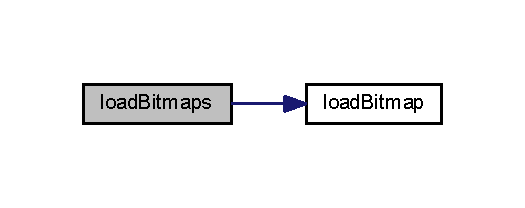
\includegraphics[width=252pt]{group__bitmaps_ga5a66eb06403c650e88bc9463e79bf9bc_cgraph}
\end{center}
\end{figure}
Here is the caller graph for this function\+:\nopagebreak
\begin{figure}[H]
\begin{center}
\leavevmode
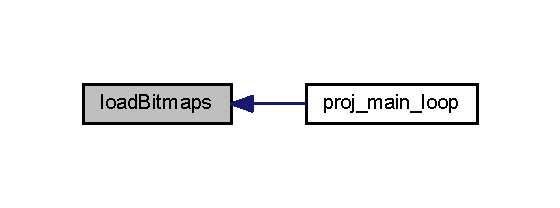
\includegraphics[width=269pt]{group__bitmaps_ga5a66eb06403c650e88bc9463e79bf9bc_icgraph}
\end{center}
\end{figure}

\hypertarget{group__canvas}{}\section{canvas}
\label{group__canvas}\index{canvas@{canvas}}
\subsection*{Classes}
\begin{DoxyCompactItemize}
\item 
struct \mbox{\hyperlink{struct_canvas}{Canvas}}
\begin{DoxyCompactList}\small\item\em Represents a canvas to draw on. \end{DoxyCompactList}\end{DoxyCompactItemize}
\subsection*{Enumerations}
\begin{DoxyCompactItemize}
\item 
enum \mbox{\hyperlink{group__canvas_ga55b506070847a13554f8b879c1bfb37c}{Shape}} \{ \mbox{\hyperlink{group__canvas_gga55b506070847a13554f8b879c1bfb37ca3f73020bb3eee4324fe1181b5a500873}{No\+Shape}} = 0, 
\mbox{\hyperlink{group__canvas_gga55b506070847a13554f8b879c1bfb37cad3ce82743a8255ccd69f5b67d257c489}{Circle}} = 1, 
\mbox{\hyperlink{group__canvas_gga55b506070847a13554f8b879c1bfb37ca65b3bc9ab39ffbf46ba5a60a0f696060}{Circumference}} = 2, 
\mbox{\hyperlink{group__canvas_gga55b506070847a13554f8b879c1bfb37cad614565f121617f9b952559339bffcf6}{Rectangle}} = 3
 \}
\end{DoxyCompactItemize}
\subsection*{Functions}
\begin{DoxyCompactItemize}
\item 
void \mbox{\hyperlink{group__canvas_ga8ca57c812327763152c635d235e3104e}{create\+\_\+canvas}} (\mbox{\hyperlink{struct_layer}{Layer}} $\ast$layer, uint16\+\_\+t x\+Min, uint16\+\_\+t y\+Min, uint16\+\_\+t x\+Max, uint16\+\_\+t y\+Max, uint32\+\_\+t \mbox{\hyperlink{structcolor}{color}})
\begin{DoxyCompactList}\small\item\em Creates a canvas and draws it on the screen, with a black outline. \end{DoxyCompactList}\item 
void \mbox{\hyperlink{group__canvas_ga1574bd14271b62f79a866c5b961ea41a}{destroy\+\_\+canvas}} ()
\begin{DoxyCompactList}\small\item\em Frees the memory used by the canvas, so that a new one can be created later. \end{DoxyCompactList}\item 
void \mbox{\hyperlink{group__canvas_ga6467ff4e7b1752b7d5e59664a16d3319}{canvas\+\_\+draw\+\_\+line}} (uint16\+\_\+t x0, uint16\+\_\+t y0, uint16\+\_\+t xf, uint16\+\_\+t yf, uint32\+\_\+t \mbox{\hyperlink{structcolor}{color}}, uint16\+\_\+t thickness)
\begin{DoxyCompactList}\small\item\em Draws a line on the canvas, updating the screen. \end{DoxyCompactList}\item 
void \mbox{\hyperlink{group__canvas_ga6cdeb1a3e72205082d77d0fb9b61b22f}{canvas\+\_\+draw\+\_\+line2}} (uint16\+\_\+t x0, uint16\+\_\+t y0, uint16\+\_\+t xf, uint16\+\_\+t yf, uint32\+\_\+t \mbox{\hyperlink{structcolor}{color}}, uint16\+\_\+t thickness)
\begin{DoxyCompactList}\small\item\em Draws a line on the canvas, updating the screen. Uses a Square pattern. \end{DoxyCompactList}\item 
void \mbox{\hyperlink{group__canvas_gabd95ad76b8189badc5d0e84de1bb8987}{canvas\+\_\+draw\+\_\+circle}} (uint16\+\_\+t x, uint16\+\_\+t y, uint16\+\_\+t radius, uint32\+\_\+t \mbox{\hyperlink{structcolor}{color}})
\begin{DoxyCompactList}\small\item\em Draws a filled circle on the canvas. \end{DoxyCompactList}\item 
void \mbox{\hyperlink{group__canvas_ga48f0ded465dd3ec65ac6b748f61f1802}{canvas\+\_\+draw\+\_\+circumference}} (uint16\+\_\+t x, uint16\+\_\+t y, uint16\+\_\+t radius, uint8\+\_\+t thickness, uint32\+\_\+t \mbox{\hyperlink{structcolor}{color}})
\begin{DoxyCompactList}\small\item\em Draws a circumference on the canvas. \end{DoxyCompactList}\item 
void \mbox{\hyperlink{group__canvas_ga5c7fe2ae7aef254a950523cd180b9d79}{canvas\+\_\+draw\+\_\+pixel}} (uint16\+\_\+t x, uint16\+\_\+t y, uint32\+\_\+t \mbox{\hyperlink{structcolor}{color}})
\begin{DoxyCompactList}\small\item\em Draws a pixel on the canvas (assuming it\textquotesingle{}s within limits) \end{DoxyCompactList}\item 
void \mbox{\hyperlink{group__canvas_ga6e24c5fefa7848e9a29d146af77356f7}{canvas\+\_\+draw\+\_\+hline}} (uint16\+\_\+t x, uint16\+\_\+t y, uint16\+\_\+t len, uint32\+\_\+t \mbox{\hyperlink{structcolor}{color}})
\begin{DoxyCompactList}\small\item\em Draws a horizontal line on the canvas. \end{DoxyCompactList}\item 
void \mbox{\hyperlink{group__canvas_gae2adf4c3c6c687a5b8885b6a2fa45b3a}{canvas\+\_\+draw\+\_\+vline}} (uint16\+\_\+t x, uint16\+\_\+t y, uint16\+\_\+t len, uint32\+\_\+t \mbox{\hyperlink{structcolor}{color}})
\begin{DoxyCompactList}\small\item\em Draws a vertical line on the canvas. \end{DoxyCompactList}\item 
void \mbox{\hyperlink{group__canvas_ga4d89ce4c1a9450f7a5ee8e1281832584}{canvas\+\_\+draw\+\_\+rectangle}} (uint16\+\_\+t x, uint16\+\_\+t y, uint16\+\_\+t width, uint16\+\_\+t height, uint32\+\_\+t \mbox{\hyperlink{structcolor}{color}})
\begin{DoxyCompactList}\small\item\em Draws a rectangle on the canvas. \end{DoxyCompactList}\item 
void \mbox{\hyperlink{group__canvas_ga5301d24065ffd6d68ead836aaeb197f3}{canvas\+\_\+draw\+\_\+rectangle\+\_\+outline}} (uint16\+\_\+t x, uint16\+\_\+t y, uint16\+\_\+t width, uint16\+\_\+t height, uint8\+\_\+t thickness, uint32\+\_\+t \mbox{\hyperlink{structcolor}{color}})
\begin{DoxyCompactList}\small\item\em Draws a rectangle outline on the canvas. \end{DoxyCompactList}\item 
void \mbox{\hyperlink{group__canvas_gaa3c801c4663518591f899050db47ad0b}{canvas\+\_\+draw\+\_\+square}} (uint16\+\_\+t x, uint16\+\_\+t y, uint16\+\_\+t side\+\_\+len, uint32\+\_\+t \mbox{\hyperlink{structcolor}{color}})
\begin{DoxyCompactList}\small\item\em Draws a square on the canvas. \end{DoxyCompactList}\item 
void \mbox{\hyperlink{group__canvas_ga303719676550209a9abd9ca6554632ae}{canvas\+\_\+draw\+\_\+image}} (\mbox{\hyperlink{struct_bitmap}{Bitmap}} $\ast$bitmap)
\begin{DoxyCompactList}\small\item\em Draws an image on the canvas. \end{DoxyCompactList}\item 
void \mbox{\hyperlink{group__canvas_ga82c276340112469fe11a819ade81ead2}{canvas\+\_\+set\+\_\+color}} (uint32\+\_\+t \mbox{\hyperlink{structcolor}{color}})
\begin{DoxyCompactList}\small\item\em Sets the canvas color, filling it. \end{DoxyCompactList}\item 
void \mbox{\hyperlink{group__canvas_ga042599a460db7bc889fdf51cb56ae732}{canvas\+\_\+set\+\_\+outline}} (uint32\+\_\+t \mbox{\hyperlink{structcolor}{color}})
\begin{DoxyCompactList}\small\item\em Sets the canvas outline (thickness 5) \end{DoxyCompactList}\item 
uint32\+\_\+t \mbox{\hyperlink{group__canvas_ga4bac68c651bfc3551d7f9fbbdf7d0e18}{rainbow}} (uint32\+\_\+t old\+\_\+color)
\begin{DoxyCompactList}\small\item\em Following a rainbow gradient, gets the next color in the gradient. \end{DoxyCompactList}\item 
void \mbox{\hyperlink{group__canvas_ga40081f7d018fdf95112d5171175fc30c}{bucket\+\_\+tool}} (uint16\+\_\+t x, uint16\+\_\+t y, uint32\+\_\+t cor\+\_\+balde)
\begin{DoxyCompactList}\small\item\em Flood fills the canvas. \end{DoxyCompactList}\item 
bool \mbox{\hyperlink{group__canvas_ga85fca0492c1f7ec8e1d20a9b5e48be1c}{is\+\_\+inside\+\_\+canvas}} (uint16\+\_\+t x, uint16\+\_\+t y)
\begin{DoxyCompactList}\small\item\em Checks if a position is inside the canvas. \end{DoxyCompactList}\item 
char $\ast$ \mbox{\hyperlink{group__canvas_gaa7891435582c7691d473ac6532e497a9}{canvas\+\_\+get\+\_\+map}} ()
\item 
int \mbox{\hyperlink{group__canvas_gac9eac428cd153893841c96d6a9ce982a}{canvas\+\_\+get\+\_\+height}} ()
\item 
int \mbox{\hyperlink{group__canvas_gaa5703f24ea2a8ec8bee2c73225c39553}{canvas\+\_\+get\+\_\+width}} ()
\item 
void \mbox{\hyperlink{group__canvas_ga62d3a3d77148b1c1ce74a7fd960601f8}{canvas\+\_\+draw\+\_\+shape}} (\mbox{\hyperlink{group__canvas_ga55b506070847a13554f8b879c1bfb37c}{Shape}} shape, uint16\+\_\+t click1\+\_\+x, uint16\+\_\+t click1\+\_\+y, uint16\+\_\+t click2\+\_\+x, uint16\+\_\+t click2\+\_\+y, uint32\+\_\+t \mbox{\hyperlink{structcolor}{color}}, uint16\+\_\+t thickness)
\begin{DoxyCompactList}\small\item\em Draws a shape on the canvas, based on two mouse clicks. \end{DoxyCompactList}\item 
void \mbox{\hyperlink{group__canvas_ga3c9ed75a75ae36bc6fc7591952fccf17}{canvas\+\_\+save\+\_\+drawing}} ()
\begin{DoxyCompactList}\small\item\em Stores the current canvas pixel map in a buffer (for the next undo action). Sets an internal is\+Drawing flag. \end{DoxyCompactList}\item 
void \mbox{\hyperlink{group__canvas_ga3a6a181542db6b70c3aadc411073943d}{canvas\+\_\+start\+\_\+drawing}} (uint16\+\_\+t x, uint16\+\_\+t y)
\begin{DoxyCompactList}\small\item\em Saves drawing for the next undo action, only if the cursor position is inside the canvas and the is\+Drawing flag is not set. \end{DoxyCompactList}\item 
void \mbox{\hyperlink{group__canvas_ga95994c1c125e70ef4d9380e80ed9c3ab}{canvas\+\_\+stop\+\_\+drawing}} ()
\begin{DoxyCompactList}\small\item\em Unsets the is\+Drawing flag. \end{DoxyCompactList}\item 
void \mbox{\hyperlink{group__canvas_ga96be607ebdf4fda25a050f017d68db93}{canvas\+\_\+undo}} ()
\begin{DoxyCompactList}\small\item\em Edits the canvas to the last saved pixel map. \end{DoxyCompactList}\item 
void \mbox{\hyperlink{group__canvas_gab462a38a3f3a612931c008e28e816a8d}{canvas\+\_\+update}} ()
\begin{DoxyCompactList}\small\item\em Updates the canvas with its layer contents. \end{DoxyCompactList}\end{DoxyCompactItemize}
\subsection*{Variables}
\begin{DoxyCompactItemize}
\item 
uint16\+\_\+t \mbox{\hyperlink{group__canvas_ga10925446227a312ac91f903acaf074e8}{Canvas\+::x\+Min}}
\item 
uint16\+\_\+t \mbox{\hyperlink{group__canvas_ga91a71d5f9030202359d000a5fb54423a}{Canvas\+::y\+Min}}
\begin{DoxyCompactList}\small\item\em Position of the upper left corner. \end{DoxyCompactList}\item 
uint16\+\_\+t \mbox{\hyperlink{group__canvas_ga423c26269827a5beb80f569ba8076ae2}{Canvas\+::x\+Max}}
\item 
uint16\+\_\+t \mbox{\hyperlink{group__canvas_ga2990194f0baef3d23cb75299cc39987d}{Canvas\+::y\+Max}}
\begin{DoxyCompactList}\small\item\em Position of the lower right corner. \end{DoxyCompactList}\item 
uint16\+\_\+t \mbox{\hyperlink{group__canvas_gaee9a970b56d8660b35047a170abc58ca}{Canvas\+::width}}
\begin{DoxyCompactList}\small\item\em \mbox{\hyperlink{struct_canvas}{Canvas}} width (redundant) \end{DoxyCompactList}\item 
uint16\+\_\+t \mbox{\hyperlink{group__canvas_ga438a71c178c014aef3de261dbc7b483e}{Canvas\+::height}}
\begin{DoxyCompactList}\small\item\em \mbox{\hyperlink{struct_canvas}{Canvas}} height (redundant) \end{DoxyCompactList}\item 
\mbox{\hyperlink{struct_layer}{Layer}} $\ast$ \mbox{\hyperlink{group__canvas_gaf72f42e64c0a72256001acc241f287ce}{Canvas\+::layer}}
\begin{DoxyCompactList}\small\item\em \mbox{\hyperlink{struct_layer}{Layer}} to draw the canvas on. \end{DoxyCompactList}\end{DoxyCompactItemize}


\subsection{Detailed Description}
Functions used to create a canvas and draw on it. 

\subsection{Enumeration Type Documentation}
\mbox{\Hypertarget{group__canvas_ga55b506070847a13554f8b879c1bfb37c}\label{group__canvas_ga55b506070847a13554f8b879c1bfb37c}} 
\index{canvas@{canvas}!Shape@{Shape}}
\index{Shape@{Shape}!canvas@{canvas}}
\subsubsection{\texorpdfstring{Shape}{Shape}}
{\footnotesize\ttfamily enum \mbox{\hyperlink{group__canvas_ga55b506070847a13554f8b879c1bfb37c}{Shape}}}

\begin{DoxyEnumFields}{Enumerator}
\raisebox{\heightof{T}}[0pt][0pt]{\index{No\+Shape@{No\+Shape}!canvas@{canvas}}\index{canvas@{canvas}!No\+Shape@{No\+Shape}}}\mbox{\Hypertarget{group__canvas_gga55b506070847a13554f8b879c1bfb37ca3f73020bb3eee4324fe1181b5a500873}\label{group__canvas_gga55b506070847a13554f8b879c1bfb37ca3f73020bb3eee4324fe1181b5a500873}} 
No\+Shape&\\
\hline

\raisebox{\heightof{T}}[0pt][0pt]{\index{Circle@{Circle}!canvas@{canvas}}\index{canvas@{canvas}!Circle@{Circle}}}\mbox{\Hypertarget{group__canvas_gga55b506070847a13554f8b879c1bfb37cad3ce82743a8255ccd69f5b67d257c489}\label{group__canvas_gga55b506070847a13554f8b879c1bfb37cad3ce82743a8255ccd69f5b67d257c489}} 
Circle&\\
\hline

\raisebox{\heightof{T}}[0pt][0pt]{\index{Circumference@{Circumference}!canvas@{canvas}}\index{canvas@{canvas}!Circumference@{Circumference}}}\mbox{\Hypertarget{group__canvas_gga55b506070847a13554f8b879c1bfb37ca65b3bc9ab39ffbf46ba5a60a0f696060}\label{group__canvas_gga55b506070847a13554f8b879c1bfb37ca65b3bc9ab39ffbf46ba5a60a0f696060}} 
Circumference&\\
\hline

\raisebox{\heightof{T}}[0pt][0pt]{\index{Rectangle@{Rectangle}!canvas@{canvas}}\index{canvas@{canvas}!Rectangle@{Rectangle}}}\mbox{\Hypertarget{group__canvas_gga55b506070847a13554f8b879c1bfb37cad614565f121617f9b952559339bffcf6}\label{group__canvas_gga55b506070847a13554f8b879c1bfb37cad614565f121617f9b952559339bffcf6}} 
Rectangle&\\
\hline

\end{DoxyEnumFields}


\subsection{Function Documentation}
\mbox{\Hypertarget{group__canvas_ga40081f7d018fdf95112d5171175fc30c}\label{group__canvas_ga40081f7d018fdf95112d5171175fc30c}} 
\index{canvas@{canvas}!bucket\+\_\+tool@{bucket\+\_\+tool}}
\index{bucket\+\_\+tool@{bucket\+\_\+tool}!canvas@{canvas}}
\subsubsection{\texorpdfstring{bucket\+\_\+tool()}{bucket\_tool()}}
{\footnotesize\ttfamily void bucket\+\_\+tool (\begin{DoxyParamCaption}\item[{uint16\+\_\+t}]{x,  }\item[{uint16\+\_\+t}]{y,  }\item[{uint32\+\_\+t}]{cor\+\_\+balde }\end{DoxyParamCaption})}



Flood fills the canvas. 


\begin{DoxyParams}{Parameters}
{\em x} & X position to flood fill \\
\hline
{\em y} & Y position to flood fill \\
\hline
{\em cor\+\_\+balde} & Color to draw with \\
\hline
\end{DoxyParams}
Here is the call graph for this function\+:\nopagebreak
\begin{figure}[H]
\begin{center}
\leavevmode
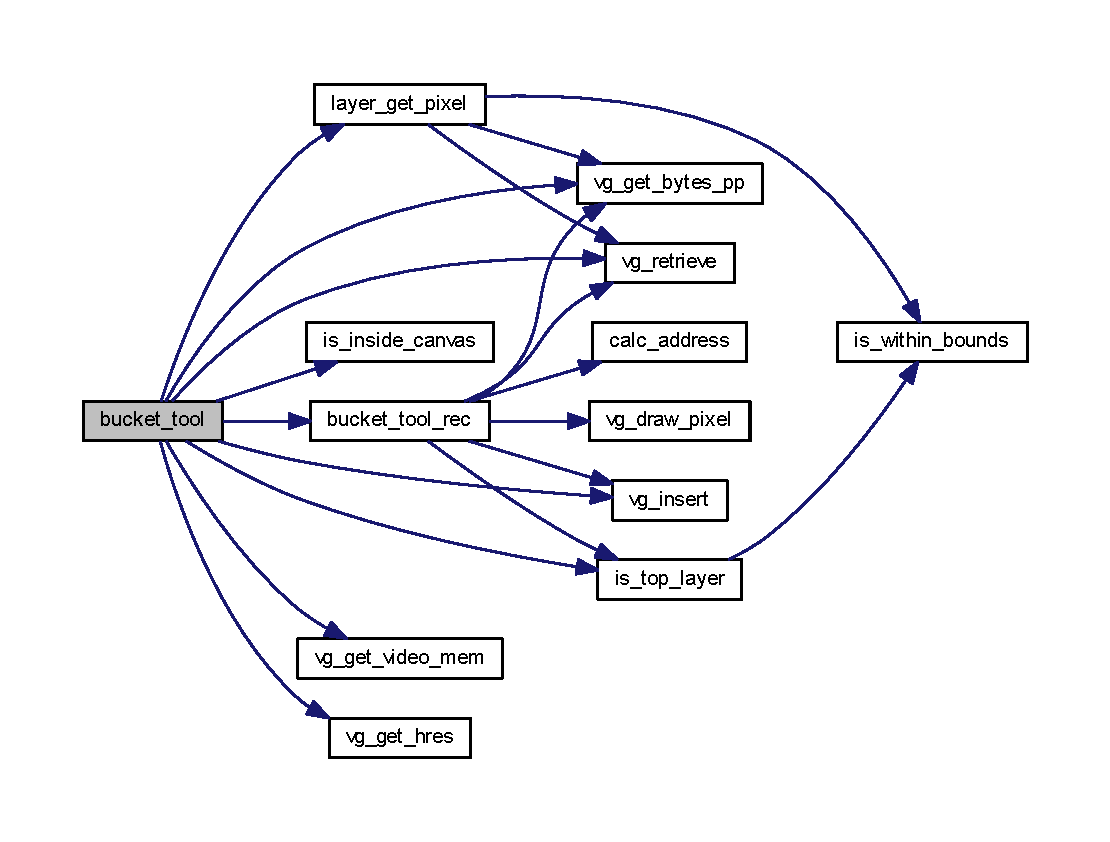
\includegraphics[width=350pt]{group__canvas_ga40081f7d018fdf95112d5171175fc30c_cgraph}
\end{center}
\end{figure}
Here is the caller graph for this function\+:\nopagebreak
\begin{figure}[H]
\begin{center}
\leavevmode
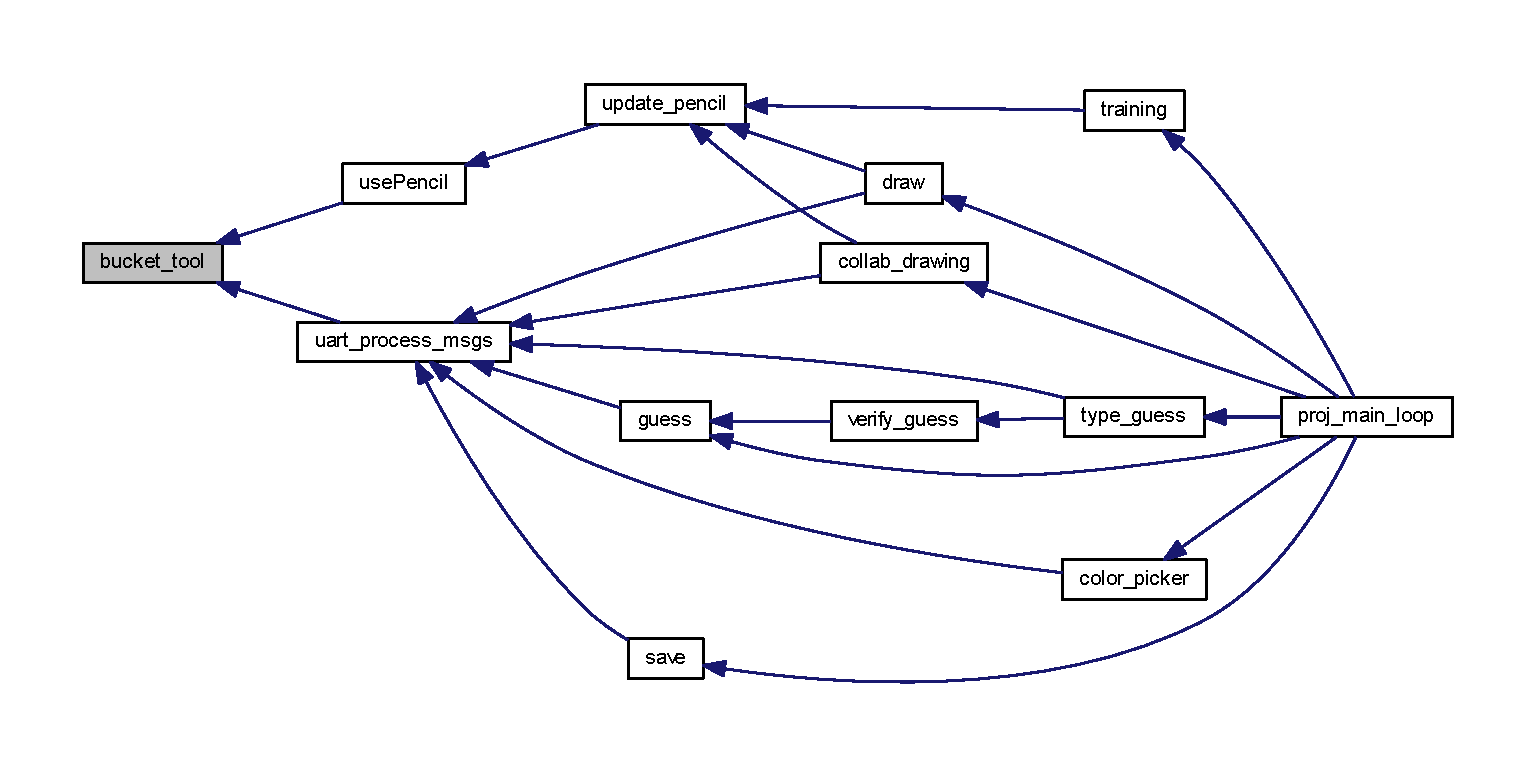
\includegraphics[width=350pt]{group__canvas_ga40081f7d018fdf95112d5171175fc30c_icgraph}
\end{center}
\end{figure}
\mbox{\Hypertarget{group__canvas_gabd95ad76b8189badc5d0e84de1bb8987}\label{group__canvas_gabd95ad76b8189badc5d0e84de1bb8987}} 
\index{canvas@{canvas}!canvas\+\_\+draw\+\_\+circle@{canvas\+\_\+draw\+\_\+circle}}
\index{canvas\+\_\+draw\+\_\+circle@{canvas\+\_\+draw\+\_\+circle}!canvas@{canvas}}
\subsubsection{\texorpdfstring{canvas\+\_\+draw\+\_\+circle()}{canvas\_draw\_circle()}}
{\footnotesize\ttfamily void canvas\+\_\+draw\+\_\+circle (\begin{DoxyParamCaption}\item[{uint16\+\_\+t}]{x,  }\item[{uint16\+\_\+t}]{y,  }\item[{uint16\+\_\+t}]{radius,  }\item[{uint32\+\_\+t}]{color }\end{DoxyParamCaption})}



Draws a filled circle on the canvas. 


\begin{DoxyParams}{Parameters}
{\em x} & X position of the center \\
\hline
{\em y} & Y position of the center \\
\hline
{\em radius} & Circle radius \\
\hline
{\em color} & Circle color \\
\hline
\end{DoxyParams}
Here is the call graph for this function\+:\nopagebreak
\begin{figure}[H]
\begin{center}
\leavevmode
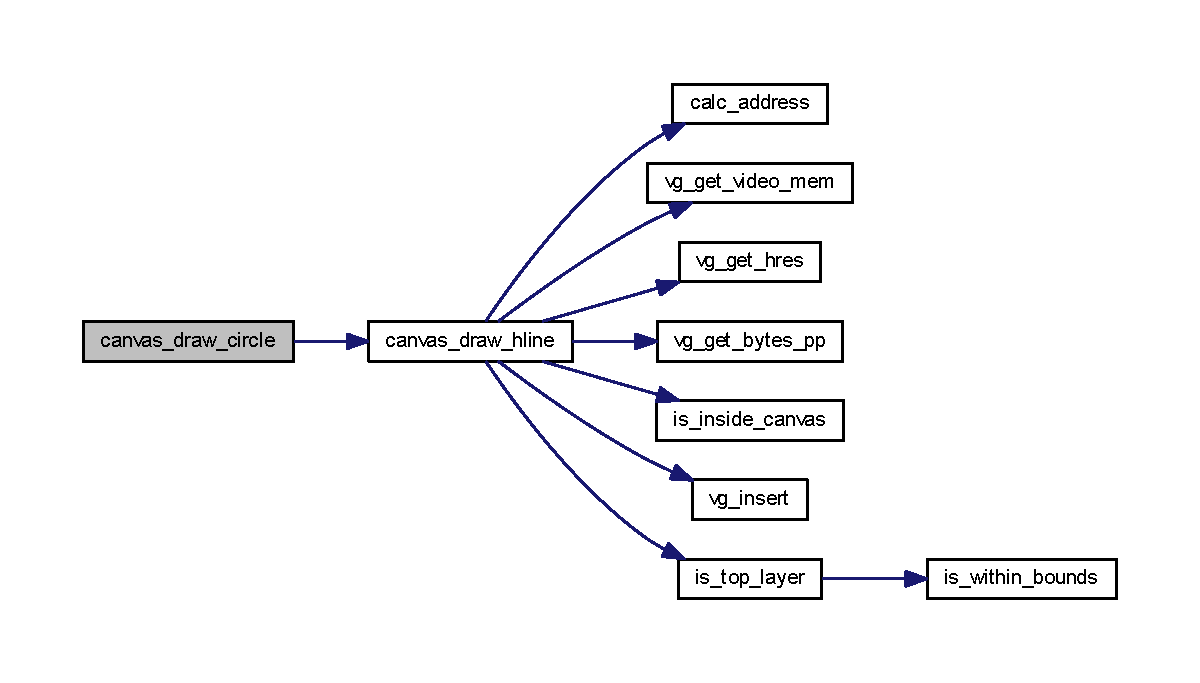
\includegraphics[width=350pt]{group__canvas_gabd95ad76b8189badc5d0e84de1bb8987_cgraph}
\end{center}
\end{figure}
Here is the caller graph for this function\+:\nopagebreak
\begin{figure}[H]
\begin{center}
\leavevmode
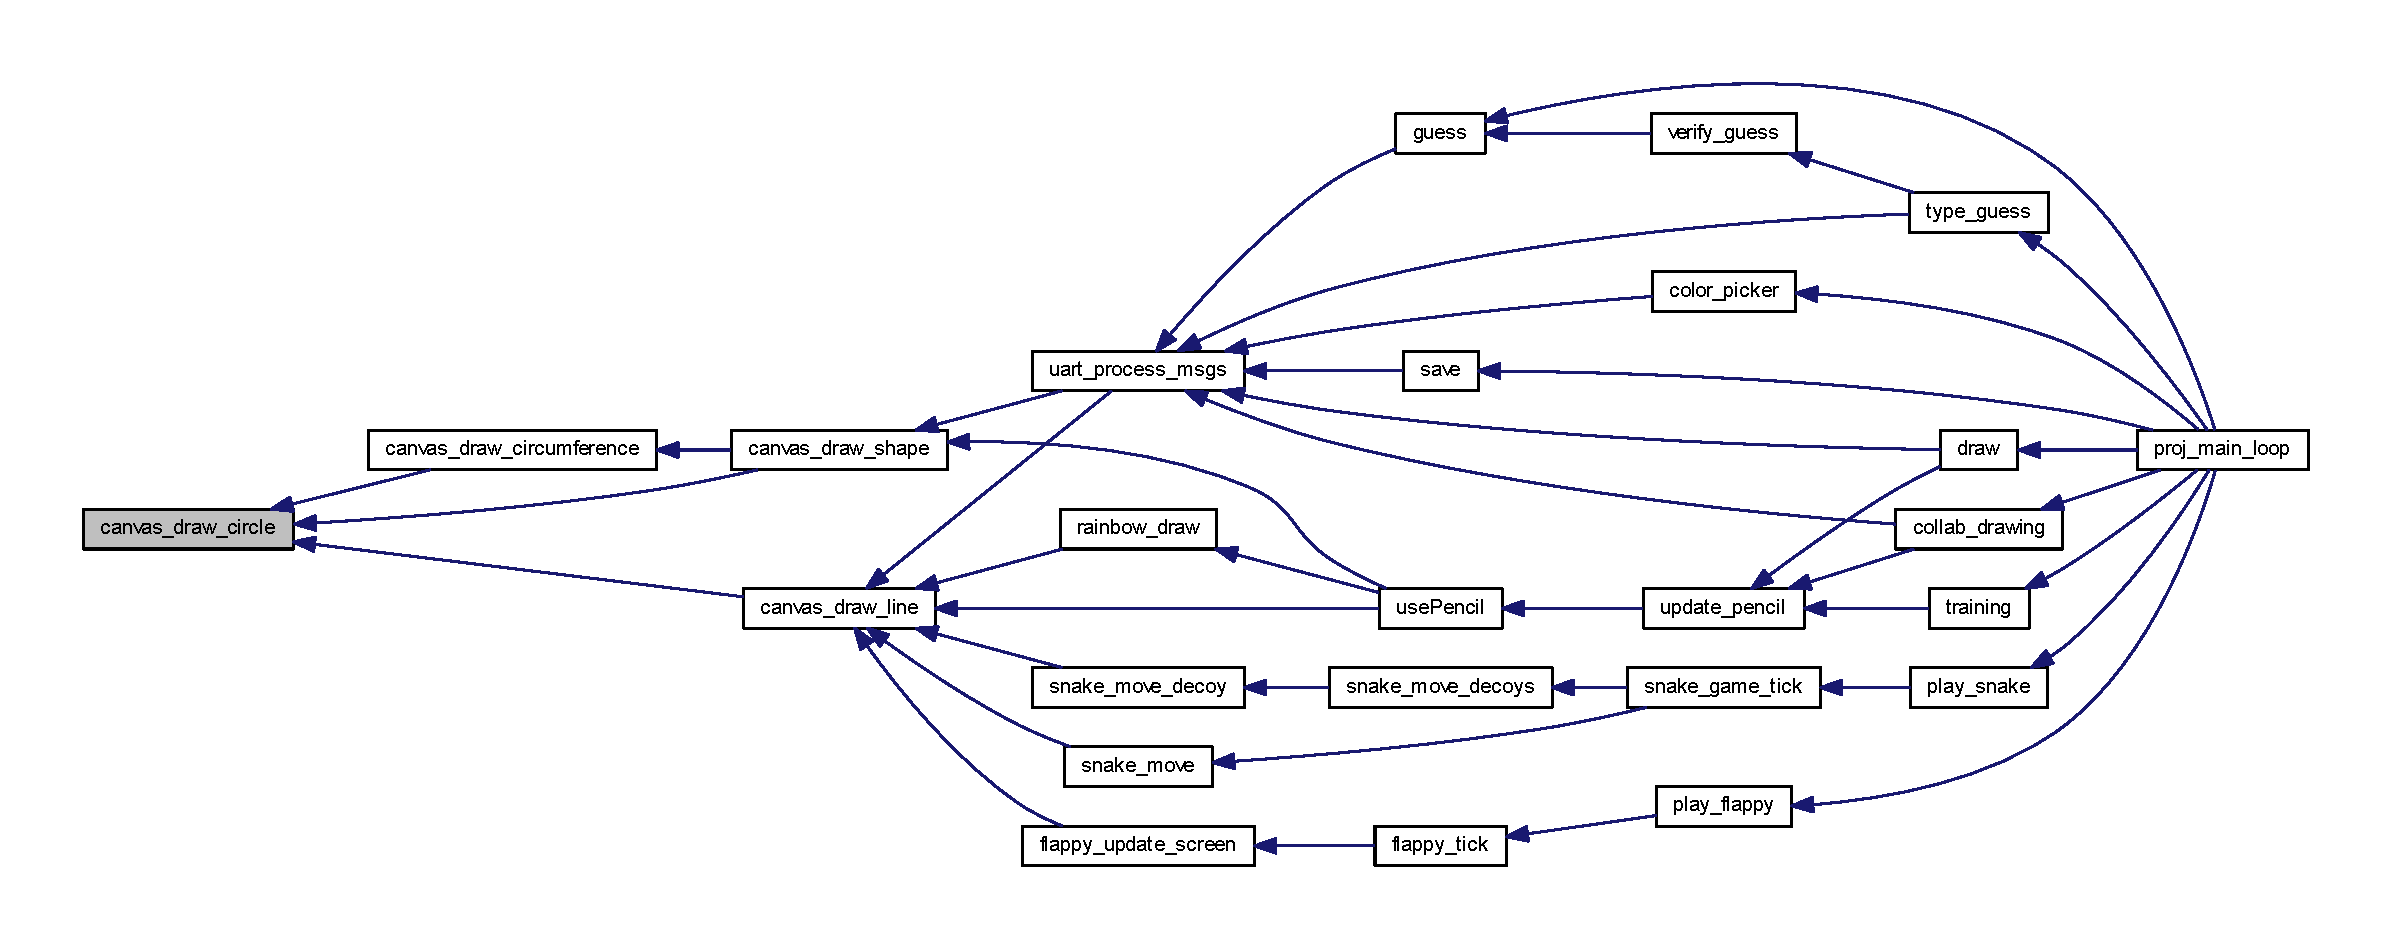
\includegraphics[width=350pt]{group__canvas_gabd95ad76b8189badc5d0e84de1bb8987_icgraph}
\end{center}
\end{figure}
\mbox{\Hypertarget{group__canvas_ga48f0ded465dd3ec65ac6b748f61f1802}\label{group__canvas_ga48f0ded465dd3ec65ac6b748f61f1802}} 
\index{canvas@{canvas}!canvas\+\_\+draw\+\_\+circumference@{canvas\+\_\+draw\+\_\+circumference}}
\index{canvas\+\_\+draw\+\_\+circumference@{canvas\+\_\+draw\+\_\+circumference}!canvas@{canvas}}
\subsubsection{\texorpdfstring{canvas\+\_\+draw\+\_\+circumference()}{canvas\_draw\_circumference()}}
{\footnotesize\ttfamily void canvas\+\_\+draw\+\_\+circumference (\begin{DoxyParamCaption}\item[{uint16\+\_\+t}]{x,  }\item[{uint16\+\_\+t}]{y,  }\item[{uint16\+\_\+t}]{radius,  }\item[{uint8\+\_\+t}]{thickness,  }\item[{uint32\+\_\+t}]{color }\end{DoxyParamCaption})}



Draws a circumference on the canvas. 


\begin{DoxyParams}{Parameters}
{\em x} & X position of the center \\
\hline
{\em y} & Y position of the center \\
\hline
{\em radius} & circumference radius \\
\hline
{\em thickness} & circumference thickness \\
\hline
{\em color} & circumference color \\
\hline
\end{DoxyParams}
Here is the call graph for this function\+:\nopagebreak
\begin{figure}[H]
\begin{center}
\leavevmode
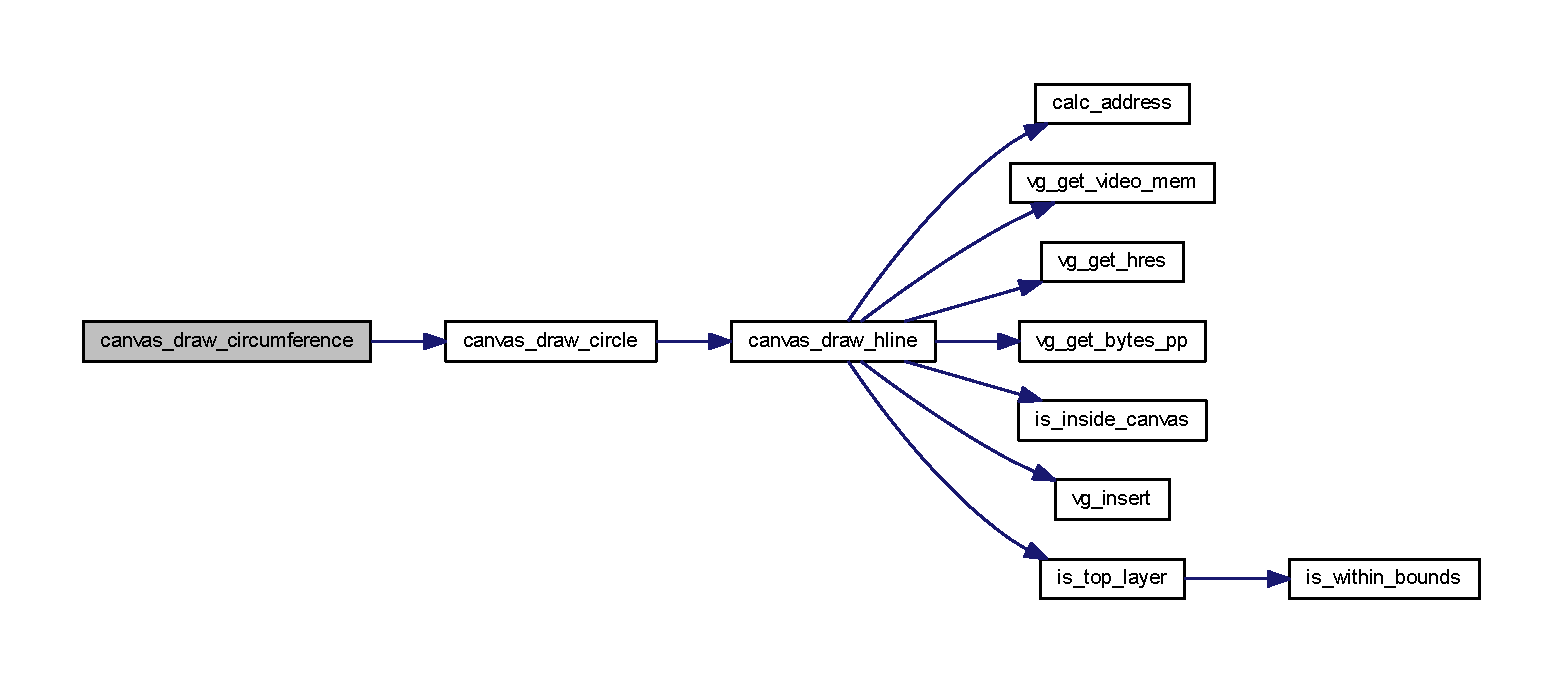
\includegraphics[width=350pt]{group__canvas_ga48f0ded465dd3ec65ac6b748f61f1802_cgraph}
\end{center}
\end{figure}
Here is the caller graph for this function\+:\nopagebreak
\begin{figure}[H]
\begin{center}
\leavevmode
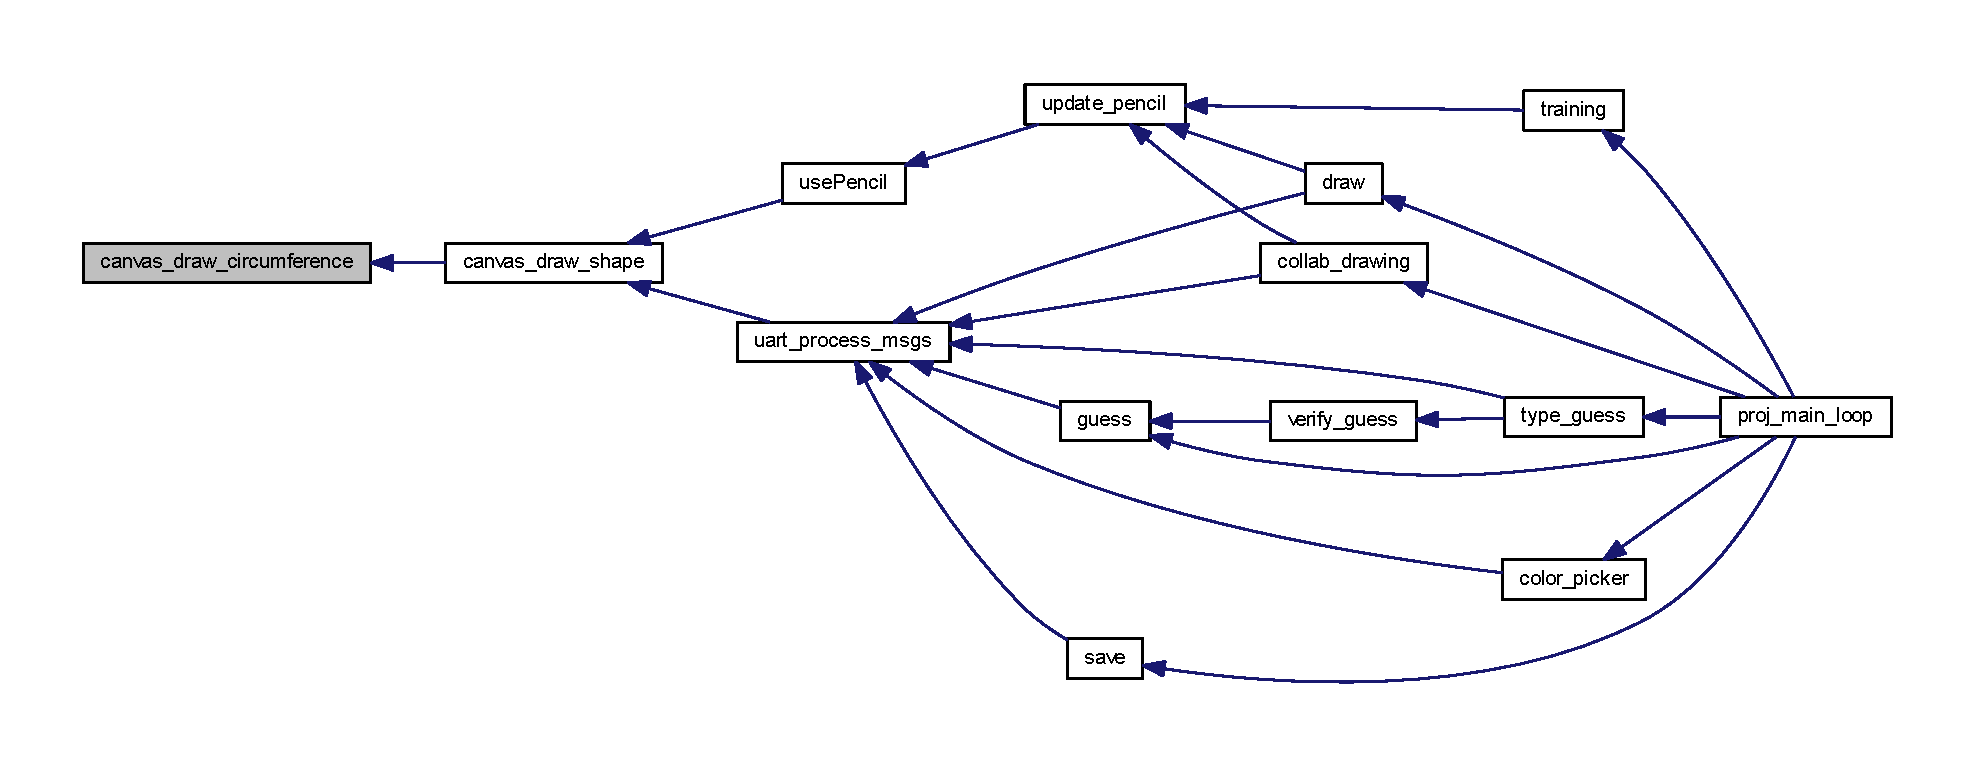
\includegraphics[width=350pt]{group__canvas_ga48f0ded465dd3ec65ac6b748f61f1802_icgraph}
\end{center}
\end{figure}
\mbox{\Hypertarget{group__canvas_ga6e24c5fefa7848e9a29d146af77356f7}\label{group__canvas_ga6e24c5fefa7848e9a29d146af77356f7}} 
\index{canvas@{canvas}!canvas\+\_\+draw\+\_\+hline@{canvas\+\_\+draw\+\_\+hline}}
\index{canvas\+\_\+draw\+\_\+hline@{canvas\+\_\+draw\+\_\+hline}!canvas@{canvas}}
\subsubsection{\texorpdfstring{canvas\+\_\+draw\+\_\+hline()}{canvas\_draw\_hline()}}
{\footnotesize\ttfamily void canvas\+\_\+draw\+\_\+hline (\begin{DoxyParamCaption}\item[{uint16\+\_\+t}]{x,  }\item[{uint16\+\_\+t}]{y,  }\item[{uint16\+\_\+t}]{len,  }\item[{uint32\+\_\+t}]{color }\end{DoxyParamCaption})}



Draws a horizontal line on the canvas. 


\begin{DoxyParams}{Parameters}
{\em x} & X position of the leftmost end \\
\hline
{\em y} & Y position of the leftmost end \\
\hline
{\em len} & Line length \\
\hline
{\em color} & Line color \\
\hline
\end{DoxyParams}
Here is the call graph for this function\+:\nopagebreak
\begin{figure}[H]
\begin{center}
\leavevmode
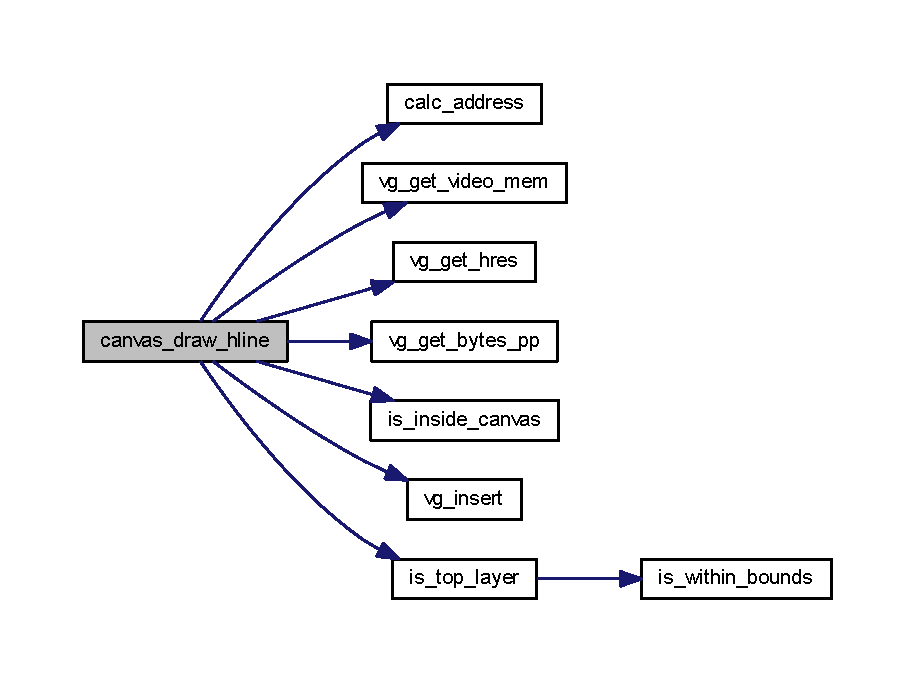
\includegraphics[width=350pt]{group__canvas_ga6e24c5fefa7848e9a29d146af77356f7_cgraph}
\end{center}
\end{figure}
Here is the caller graph for this function\+:\nopagebreak
\begin{figure}[H]
\begin{center}
\leavevmode
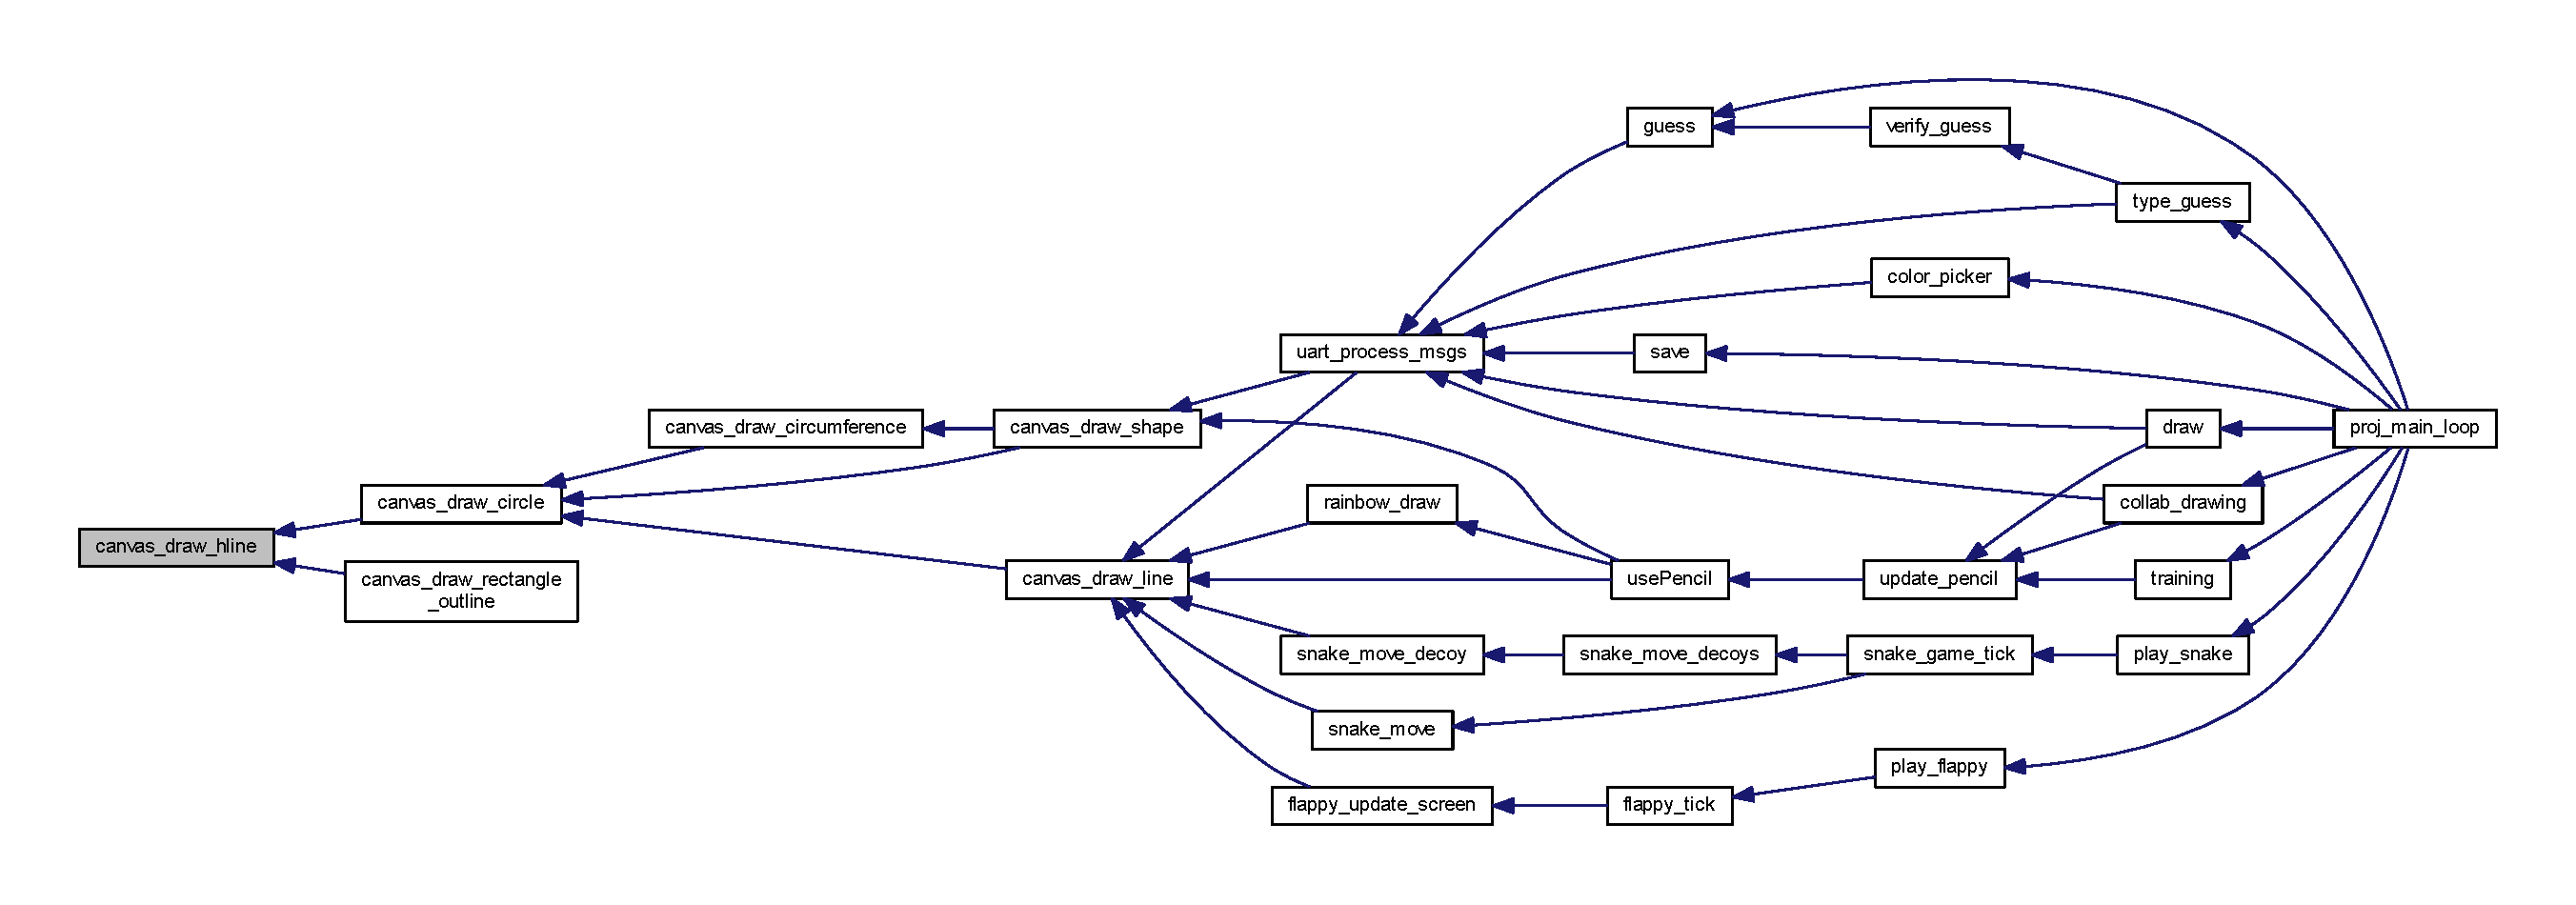
\includegraphics[width=350pt]{group__canvas_ga6e24c5fefa7848e9a29d146af77356f7_icgraph}
\end{center}
\end{figure}
\mbox{\Hypertarget{group__canvas_ga303719676550209a9abd9ca6554632ae}\label{group__canvas_ga303719676550209a9abd9ca6554632ae}} 
\index{canvas@{canvas}!canvas\+\_\+draw\+\_\+image@{canvas\+\_\+draw\+\_\+image}}
\index{canvas\+\_\+draw\+\_\+image@{canvas\+\_\+draw\+\_\+image}!canvas@{canvas}}
\subsubsection{\texorpdfstring{canvas\+\_\+draw\+\_\+image()}{canvas\_draw\_image()}}
{\footnotesize\ttfamily void canvas\+\_\+draw\+\_\+image (\begin{DoxyParamCaption}\item[{\mbox{\hyperlink{struct_bitmap}{Bitmap}} $\ast$}]{bitmap }\end{DoxyParamCaption})}



Draws an image on the canvas. 


\begin{DoxyParams}{Parameters}
{\em bitmap} & \mbox{\hyperlink{struct_bitmap}{Bitmap}} to be drawn \\
\hline
\end{DoxyParams}
Here is the call graph for this function\+:\nopagebreak
\begin{figure}[H]
\begin{center}
\leavevmode
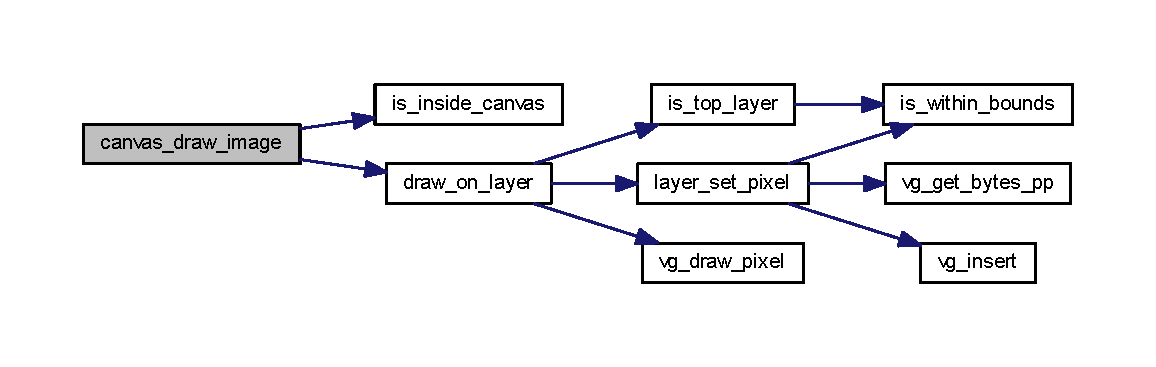
\includegraphics[width=350pt]{group__canvas_ga303719676550209a9abd9ca6554632ae_cgraph}
\end{center}
\end{figure}
Here is the caller graph for this function\+:\nopagebreak
\begin{figure}[H]
\begin{center}
\leavevmode
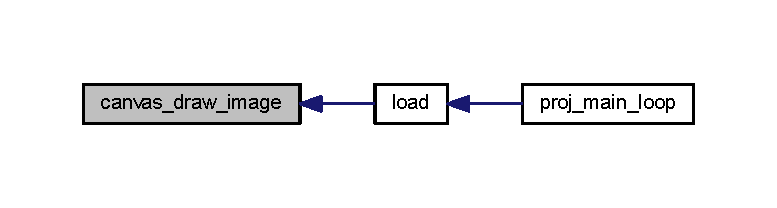
\includegraphics[width=350pt]{group__canvas_ga303719676550209a9abd9ca6554632ae_icgraph}
\end{center}
\end{figure}
\mbox{\Hypertarget{group__canvas_ga6467ff4e7b1752b7d5e59664a16d3319}\label{group__canvas_ga6467ff4e7b1752b7d5e59664a16d3319}} 
\index{canvas@{canvas}!canvas\+\_\+draw\+\_\+line@{canvas\+\_\+draw\+\_\+line}}
\index{canvas\+\_\+draw\+\_\+line@{canvas\+\_\+draw\+\_\+line}!canvas@{canvas}}
\subsubsection{\texorpdfstring{canvas\+\_\+draw\+\_\+line()}{canvas\_draw\_line()}}
{\footnotesize\ttfamily void canvas\+\_\+draw\+\_\+line (\begin{DoxyParamCaption}\item[{uint16\+\_\+t}]{x0,  }\item[{uint16\+\_\+t}]{y0,  }\item[{uint16\+\_\+t}]{xf,  }\item[{uint16\+\_\+t}]{yf,  }\item[{uint32\+\_\+t}]{color,  }\item[{uint16\+\_\+t}]{thickness }\end{DoxyParamCaption})}



Draws a line on the canvas, updating the screen. 


\begin{DoxyParams}{Parameters}
{\em x0} & X position of the left most end \\
\hline
{\em y0} & Y position of the leftmost end \\
\hline
{\em xf} & X position of the rightmost end \\
\hline
{\em yf} & Y position of the rightmost end \\
\hline
{\em color} & Color to draw the line with \\
\hline
{\em thickness} & Line thickness \\
\hline
\end{DoxyParams}
Here is the call graph for this function\+:\nopagebreak
\begin{figure}[H]
\begin{center}
\leavevmode
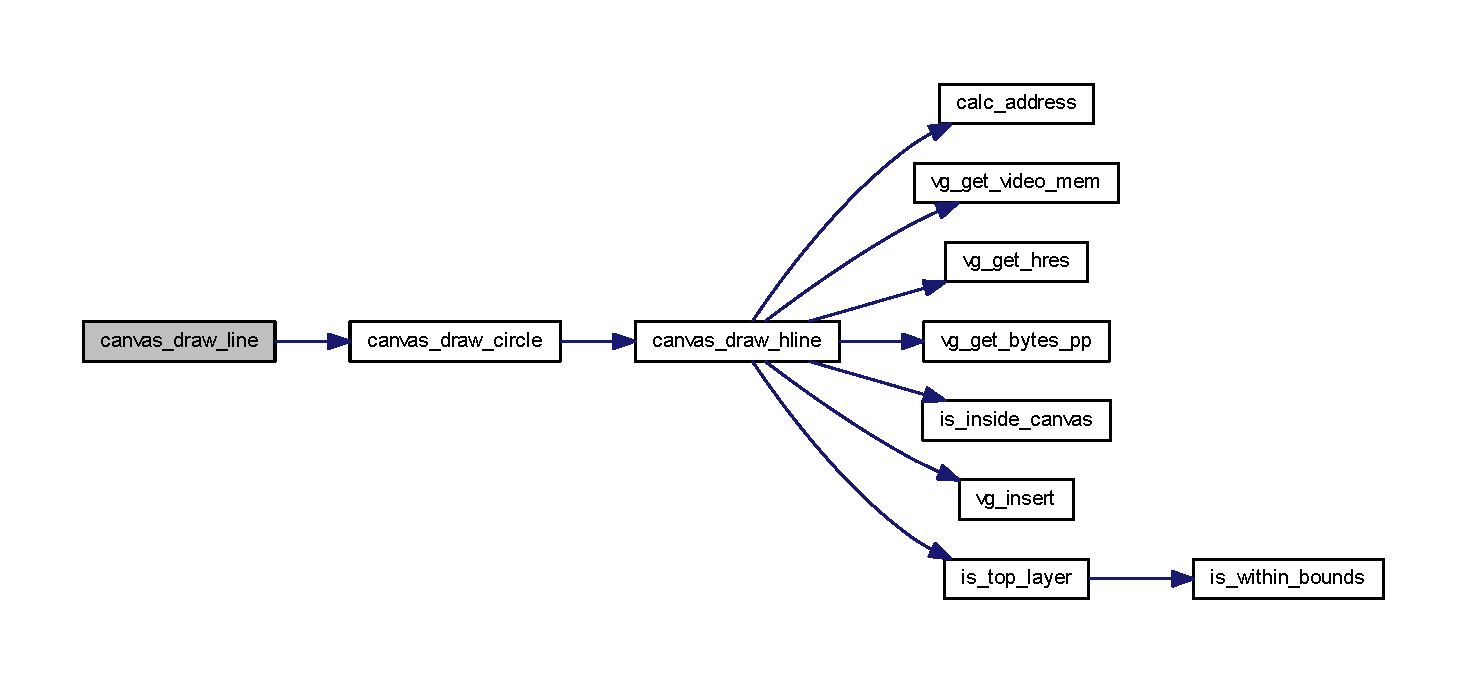
\includegraphics[width=350pt]{group__canvas_ga6467ff4e7b1752b7d5e59664a16d3319_cgraph}
\end{center}
\end{figure}
Here is the caller graph for this function\+:\nopagebreak
\begin{figure}[H]
\begin{center}
\leavevmode
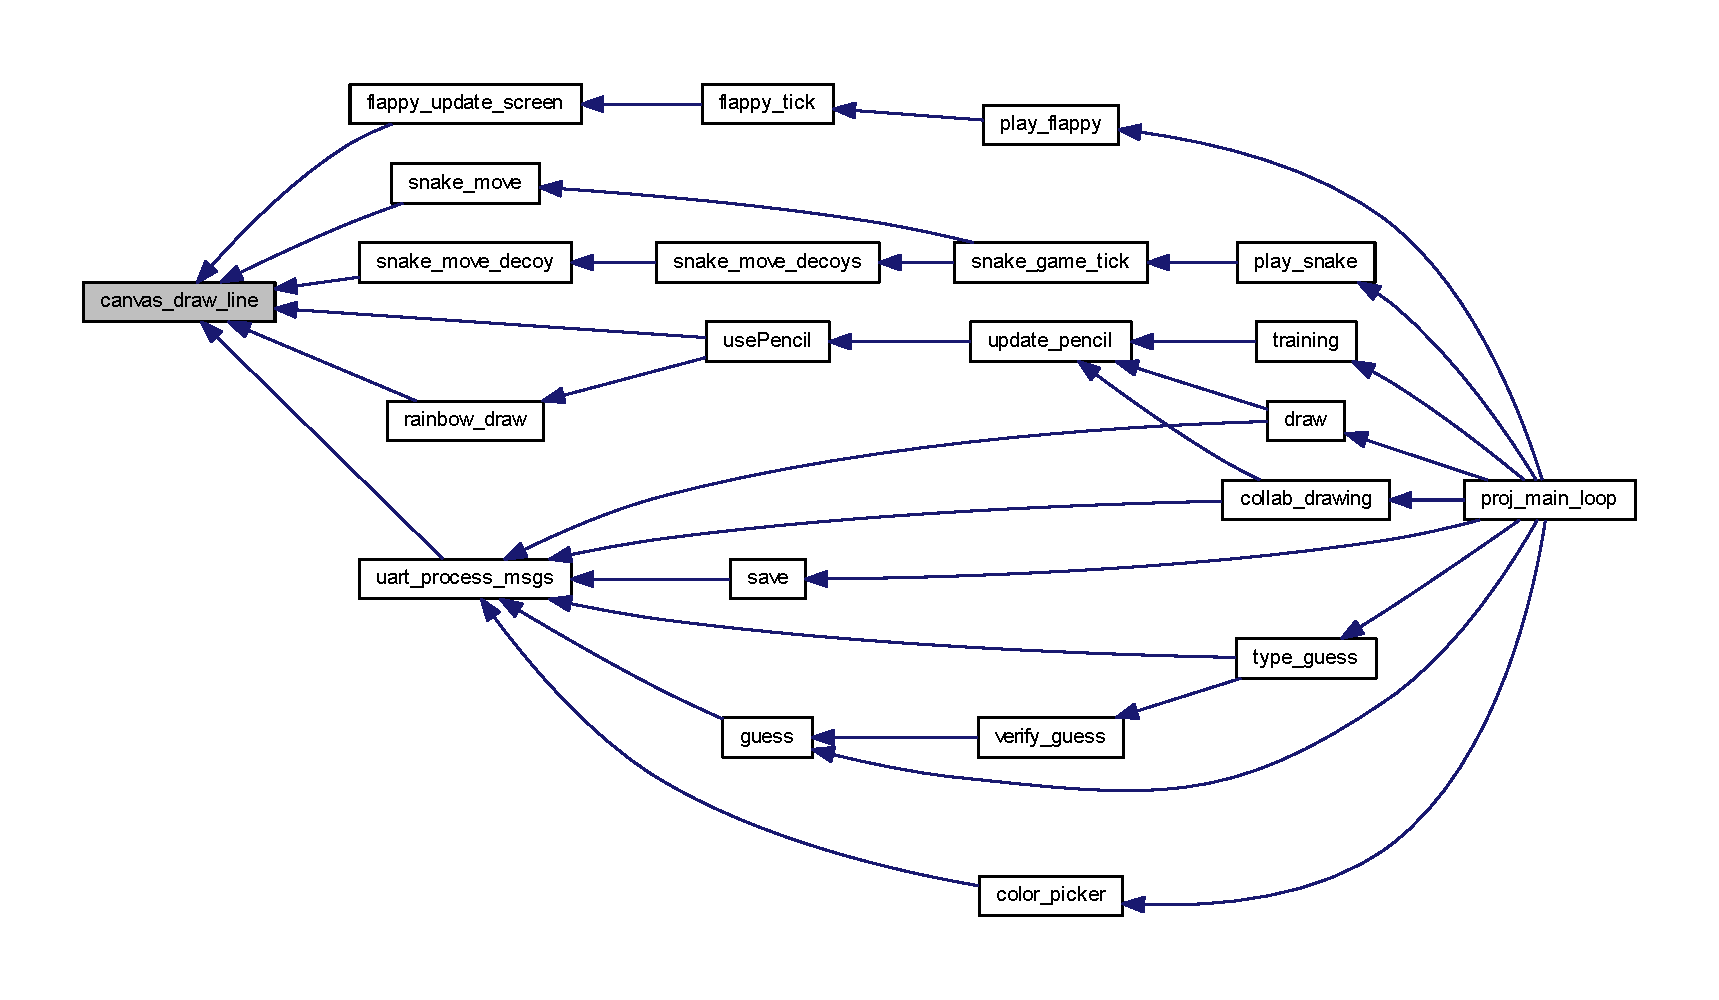
\includegraphics[width=350pt]{group__canvas_ga6467ff4e7b1752b7d5e59664a16d3319_icgraph}
\end{center}
\end{figure}
\mbox{\Hypertarget{group__canvas_ga6cdeb1a3e72205082d77d0fb9b61b22f}\label{group__canvas_ga6cdeb1a3e72205082d77d0fb9b61b22f}} 
\index{canvas@{canvas}!canvas\+\_\+draw\+\_\+line2@{canvas\+\_\+draw\+\_\+line2}}
\index{canvas\+\_\+draw\+\_\+line2@{canvas\+\_\+draw\+\_\+line2}!canvas@{canvas}}
\subsubsection{\texorpdfstring{canvas\+\_\+draw\+\_\+line2()}{canvas\_draw\_line2()}}
{\footnotesize\ttfamily void canvas\+\_\+draw\+\_\+line2 (\begin{DoxyParamCaption}\item[{uint16\+\_\+t}]{x0,  }\item[{uint16\+\_\+t}]{y0,  }\item[{uint16\+\_\+t}]{xf,  }\item[{uint16\+\_\+t}]{yf,  }\item[{uint32\+\_\+t}]{color,  }\item[{uint16\+\_\+t}]{thickness }\end{DoxyParamCaption})}



Draws a line on the canvas, updating the screen. Uses a Square pattern. 


\begin{DoxyParams}{Parameters}
{\em x0} & X position of the left most end \\
\hline
{\em y0} & Y position of the leftmost end \\
\hline
{\em xf} & X position of the rightmost end \\
\hline
{\em yf} & Y position of the rightmost end \\
\hline
{\em color} & Color to draw the line with \\
\hline
{\em thickness} & Line thickness \\
\hline
\end{DoxyParams}
Here is the call graph for this function\+:\nopagebreak
\begin{figure}[H]
\begin{center}
\leavevmode
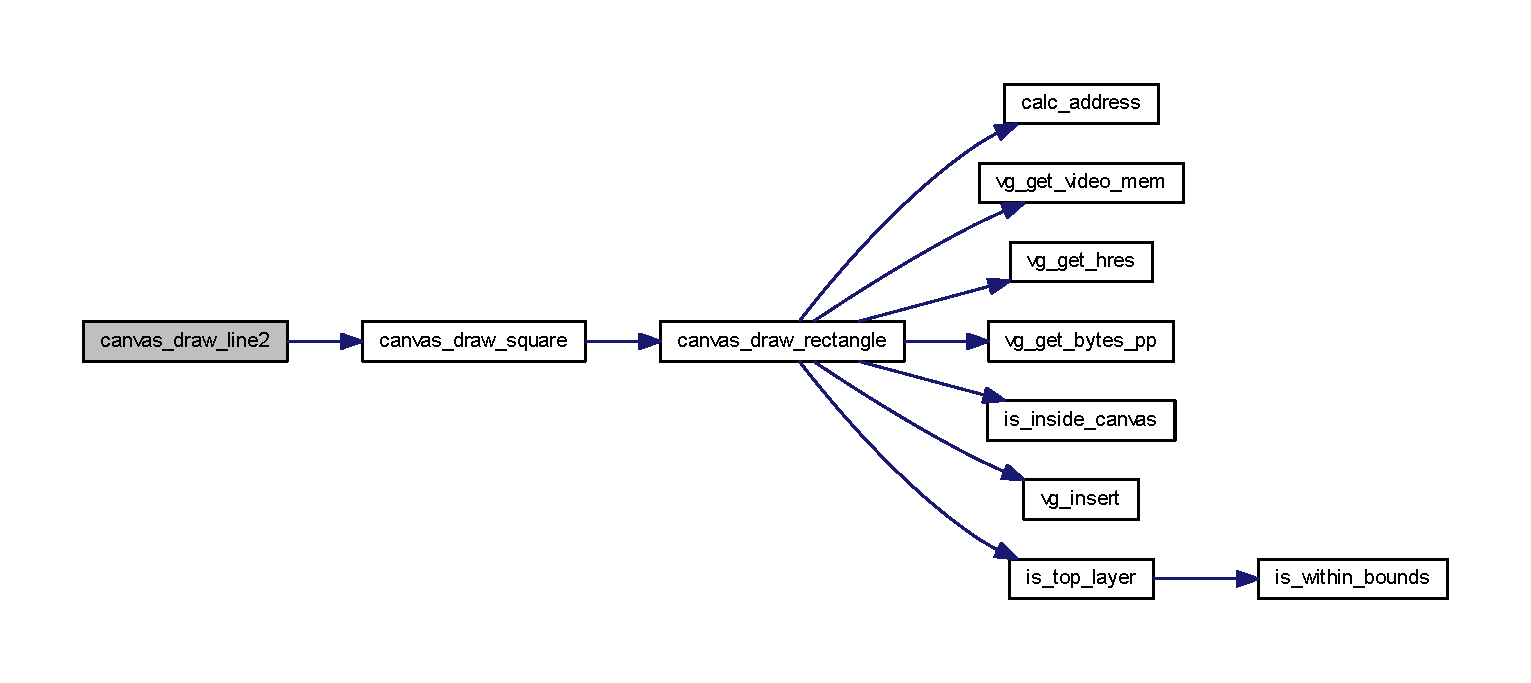
\includegraphics[width=350pt]{group__canvas_ga6cdeb1a3e72205082d77d0fb9b61b22f_cgraph}
\end{center}
\end{figure}
Here is the caller graph for this function\+:\nopagebreak
\begin{figure}[H]
\begin{center}
\leavevmode
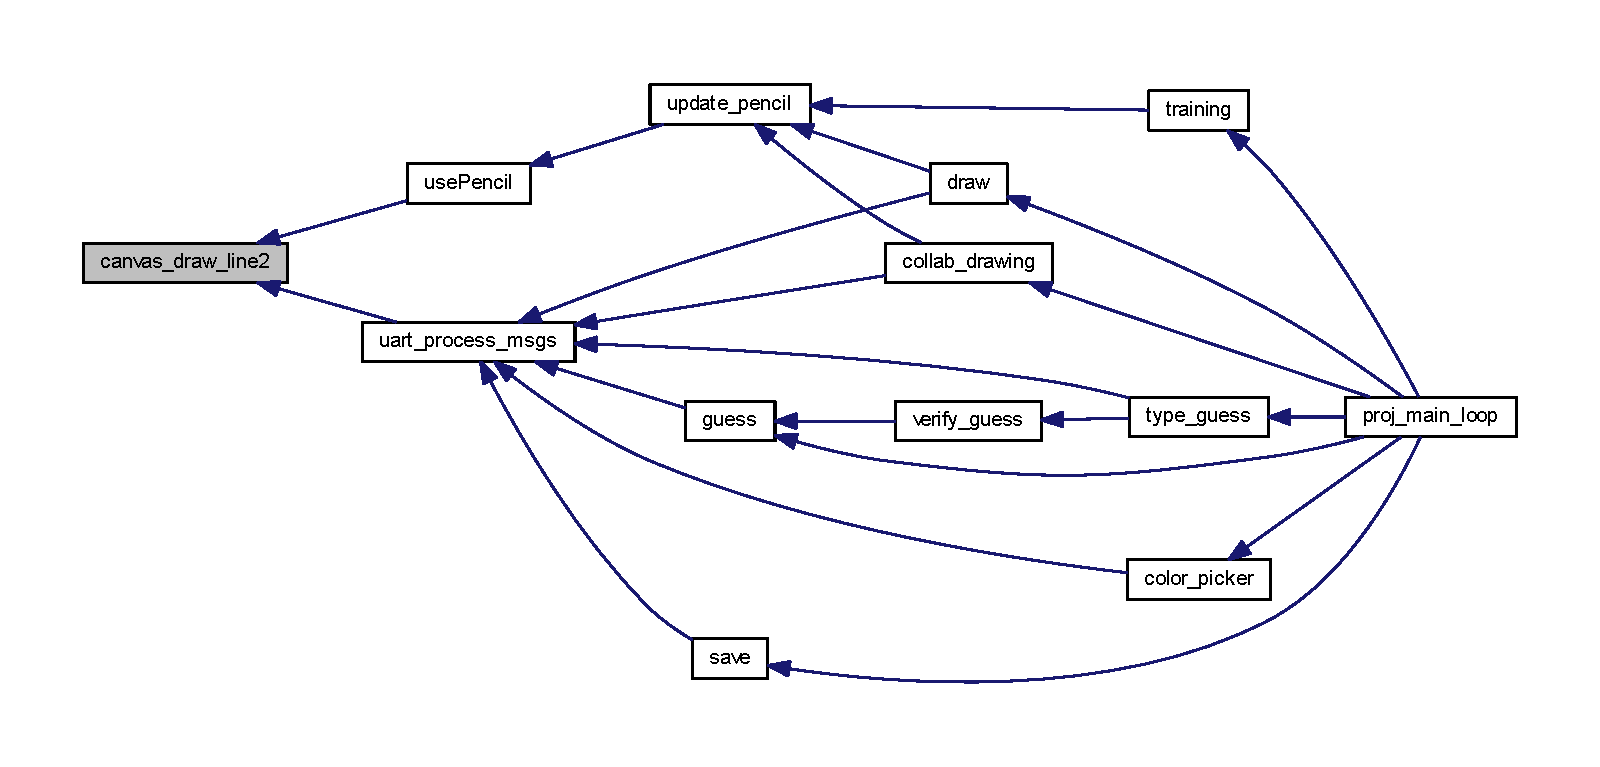
\includegraphics[width=350pt]{group__canvas_ga6cdeb1a3e72205082d77d0fb9b61b22f_icgraph}
\end{center}
\end{figure}
\mbox{\Hypertarget{group__canvas_ga5c7fe2ae7aef254a950523cd180b9d79}\label{group__canvas_ga5c7fe2ae7aef254a950523cd180b9d79}} 
\index{canvas@{canvas}!canvas\+\_\+draw\+\_\+pixel@{canvas\+\_\+draw\+\_\+pixel}}
\index{canvas\+\_\+draw\+\_\+pixel@{canvas\+\_\+draw\+\_\+pixel}!canvas@{canvas}}
\subsubsection{\texorpdfstring{canvas\+\_\+draw\+\_\+pixel()}{canvas\_draw\_pixel()}}
{\footnotesize\ttfamily void canvas\+\_\+draw\+\_\+pixel (\begin{DoxyParamCaption}\item[{uint16\+\_\+t}]{x,  }\item[{uint16\+\_\+t}]{y,  }\item[{uint32\+\_\+t}]{color }\end{DoxyParamCaption})}



Draws a pixel on the canvas (assuming it\textquotesingle{}s within limits) 


\begin{DoxyParams}{Parameters}
{\em x} & X position of the pixel \\
\hline
{\em y} & Y position of the pixel \\
\hline
{\em color} & Pixel color \\
\hline
\end{DoxyParams}
Here is the call graph for this function\+:\nopagebreak
\begin{figure}[H]
\begin{center}
\leavevmode
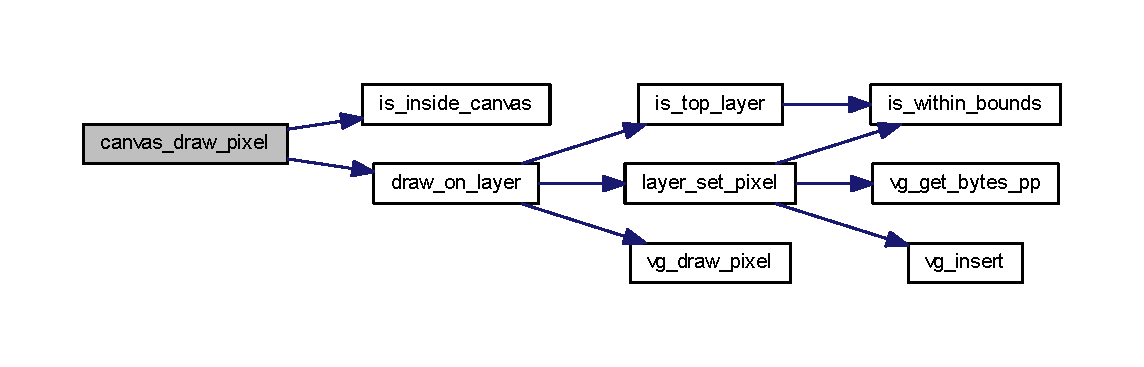
\includegraphics[width=350pt]{group__canvas_ga5c7fe2ae7aef254a950523cd180b9d79_cgraph}
\end{center}
\end{figure}
Here is the caller graph for this function\+:\nopagebreak
\begin{figure}[H]
\begin{center}
\leavevmode
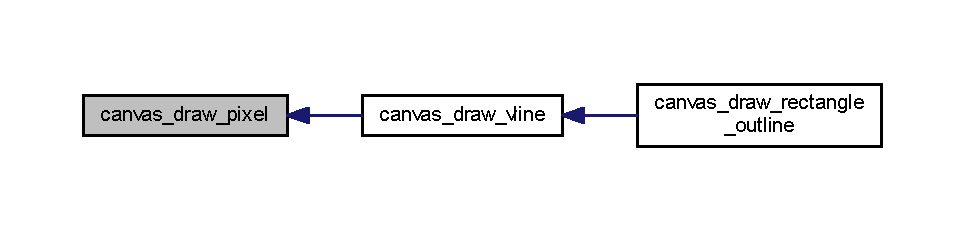
\includegraphics[width=350pt]{group__canvas_ga5c7fe2ae7aef254a950523cd180b9d79_icgraph}
\end{center}
\end{figure}
\mbox{\Hypertarget{group__canvas_ga4d89ce4c1a9450f7a5ee8e1281832584}\label{group__canvas_ga4d89ce4c1a9450f7a5ee8e1281832584}} 
\index{canvas@{canvas}!canvas\+\_\+draw\+\_\+rectangle@{canvas\+\_\+draw\+\_\+rectangle}}
\index{canvas\+\_\+draw\+\_\+rectangle@{canvas\+\_\+draw\+\_\+rectangle}!canvas@{canvas}}
\subsubsection{\texorpdfstring{canvas\+\_\+draw\+\_\+rectangle()}{canvas\_draw\_rectangle()}}
{\footnotesize\ttfamily void canvas\+\_\+draw\+\_\+rectangle (\begin{DoxyParamCaption}\item[{uint16\+\_\+t}]{x,  }\item[{uint16\+\_\+t}]{y,  }\item[{uint16\+\_\+t}]{width,  }\item[{uint16\+\_\+t}]{height,  }\item[{uint32\+\_\+t}]{color }\end{DoxyParamCaption})}



Draws a rectangle on the canvas. 


\begin{DoxyParams}{Parameters}
{\em x} & X Position of the upper left corner \\
\hline
{\em y} & Y Position of the upper left corner \\
\hline
{\em width} & Rectangle width \\
\hline
{\em height} & Rectangle height \\
\hline
{\em color} & Rectangle color \\
\hline
\end{DoxyParams}
Here is the call graph for this function\+:\nopagebreak
\begin{figure}[H]
\begin{center}
\leavevmode
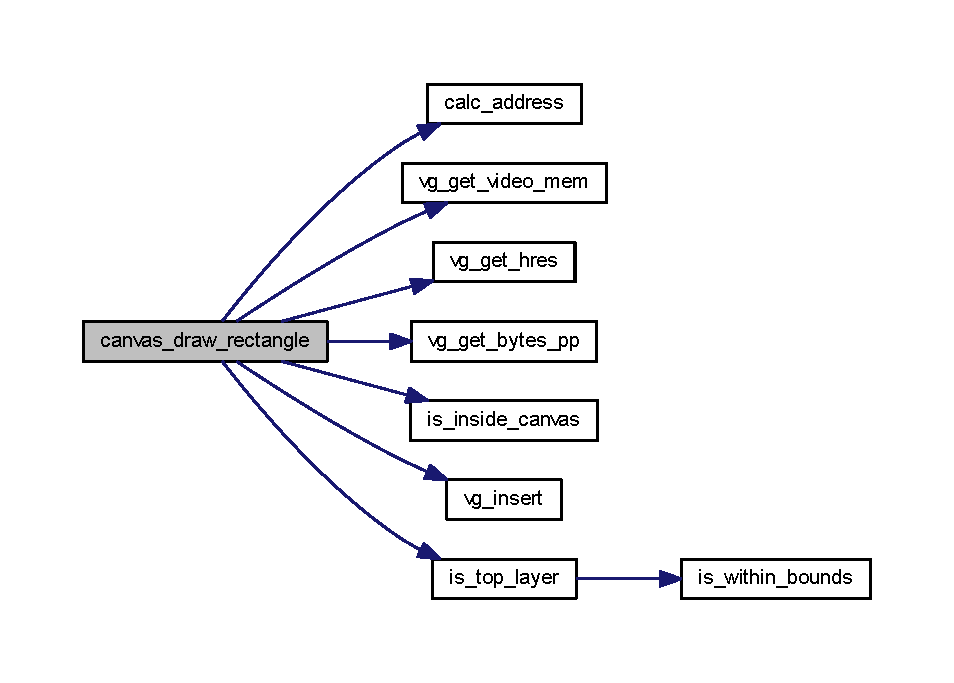
\includegraphics[width=350pt]{group__canvas_ga4d89ce4c1a9450f7a5ee8e1281832584_cgraph}
\end{center}
\end{figure}
Here is the caller graph for this function\+:\nopagebreak
\begin{figure}[H]
\begin{center}
\leavevmode
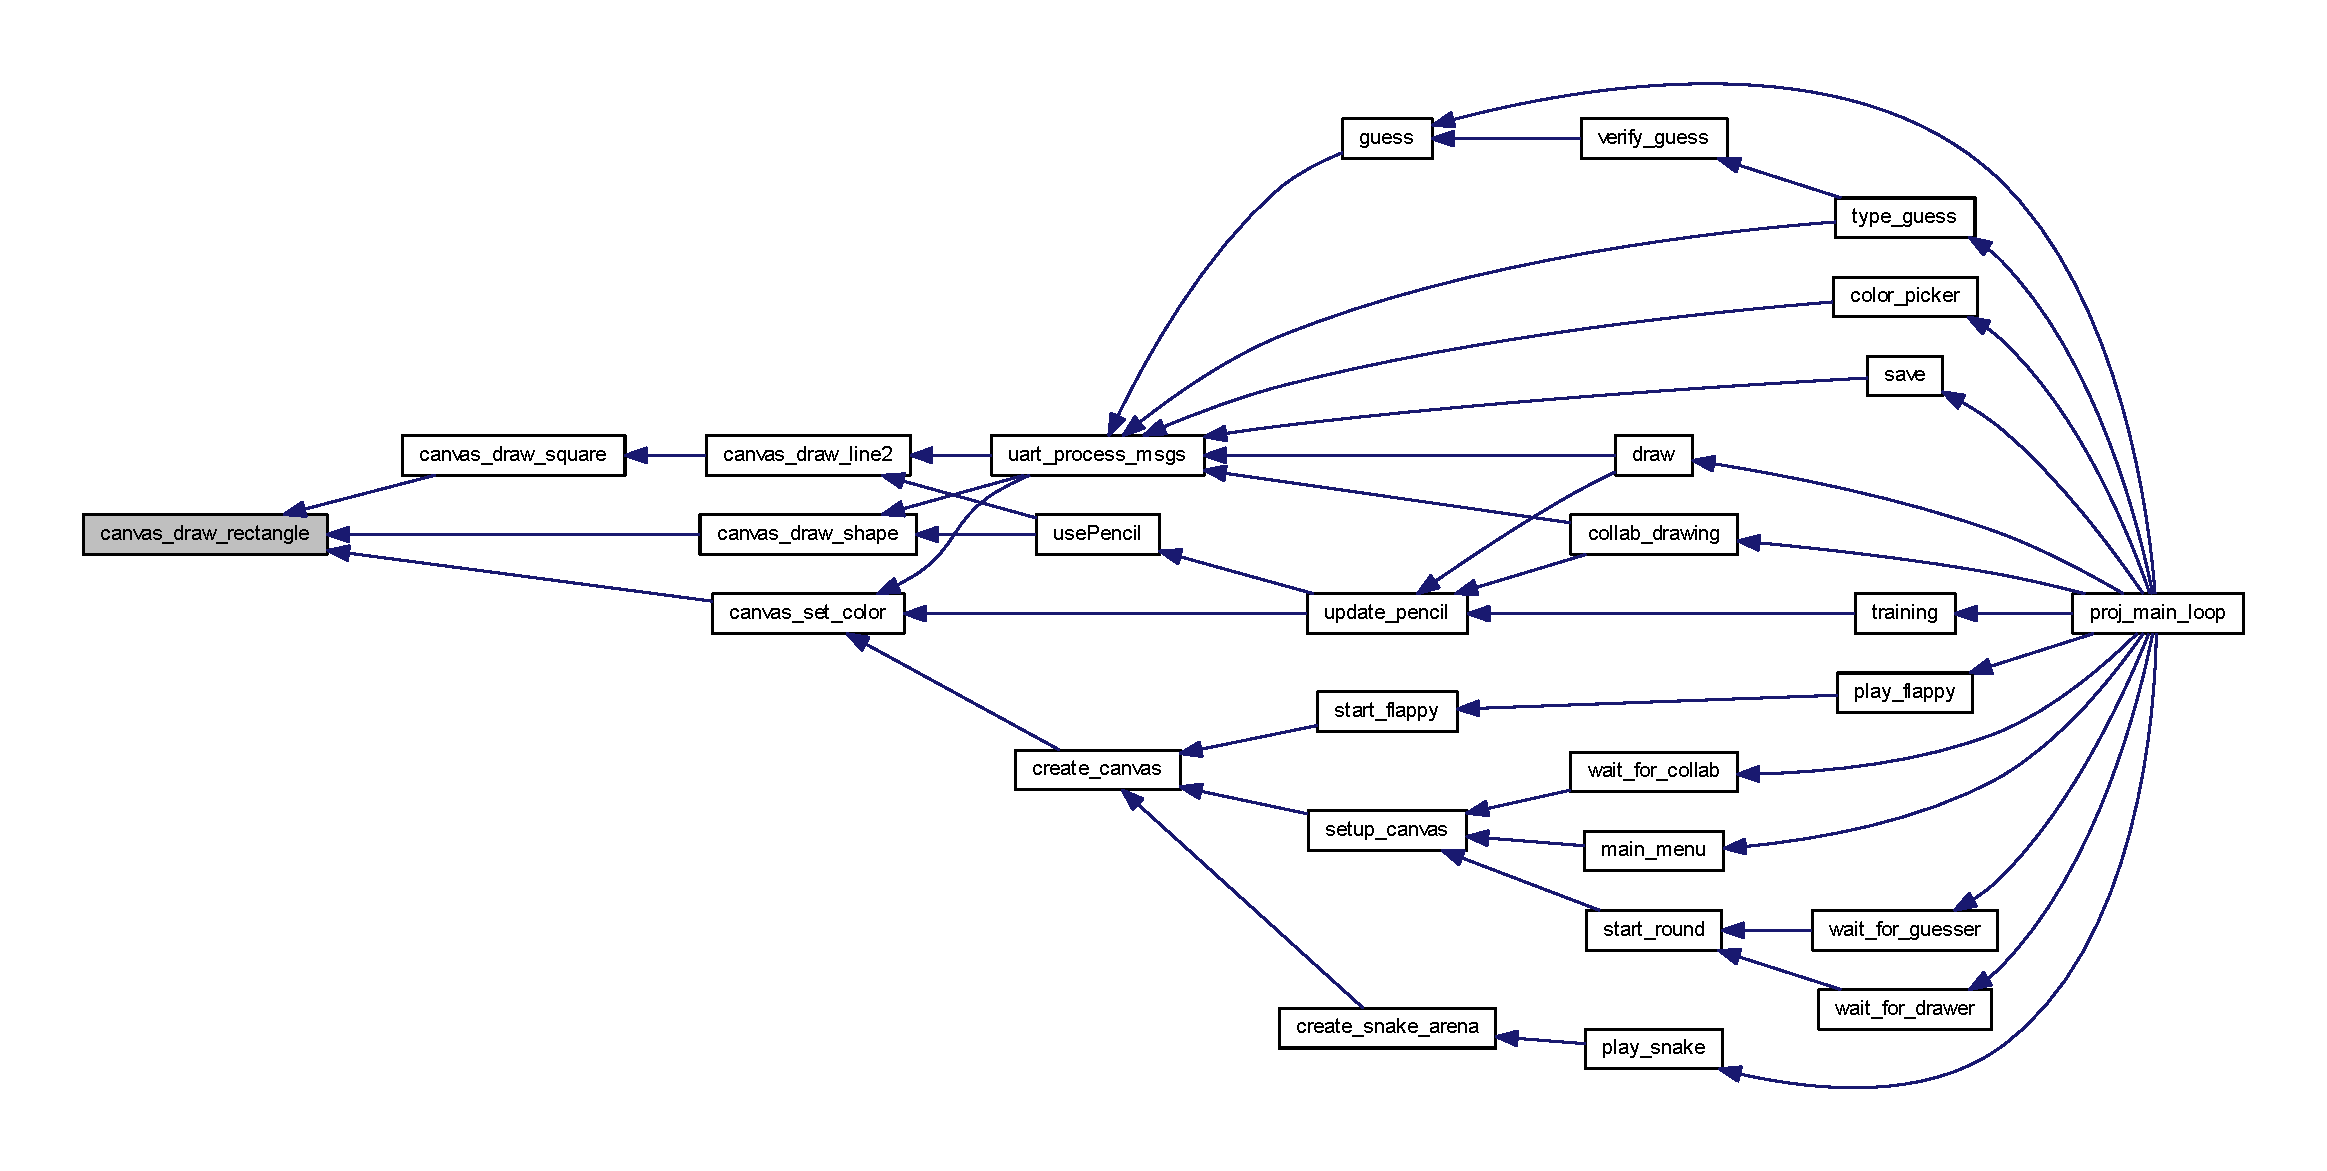
\includegraphics[width=350pt]{group__canvas_ga4d89ce4c1a9450f7a5ee8e1281832584_icgraph}
\end{center}
\end{figure}
\mbox{\Hypertarget{group__canvas_ga5301d24065ffd6d68ead836aaeb197f3}\label{group__canvas_ga5301d24065ffd6d68ead836aaeb197f3}} 
\index{canvas@{canvas}!canvas\+\_\+draw\+\_\+rectangle\+\_\+outline@{canvas\+\_\+draw\+\_\+rectangle\+\_\+outline}}
\index{canvas\+\_\+draw\+\_\+rectangle\+\_\+outline@{canvas\+\_\+draw\+\_\+rectangle\+\_\+outline}!canvas@{canvas}}
\subsubsection{\texorpdfstring{canvas\+\_\+draw\+\_\+rectangle\+\_\+outline()}{canvas\_draw\_rectangle\_outline()}}
{\footnotesize\ttfamily void canvas\+\_\+draw\+\_\+rectangle\+\_\+outline (\begin{DoxyParamCaption}\item[{uint16\+\_\+t}]{x,  }\item[{uint16\+\_\+t}]{y,  }\item[{uint16\+\_\+t}]{width,  }\item[{uint16\+\_\+t}]{height,  }\item[{uint8\+\_\+t}]{thickness,  }\item[{uint32\+\_\+t}]{color }\end{DoxyParamCaption})}



Draws a rectangle outline on the canvas. 


\begin{DoxyParams}{Parameters}
{\em x} & X Position of the upper left corner \\
\hline
{\em y} & Y Position of the upper left corner \\
\hline
{\em width} & Rectangle width \\
\hline
{\em height} & Rectangle height \\
\hline
{\em thickness} & Outline thickness \\
\hline
{\em color} & Rectangle color \\
\hline
\end{DoxyParams}
Here is the call graph for this function\+:\nopagebreak
\begin{figure}[H]
\begin{center}
\leavevmode
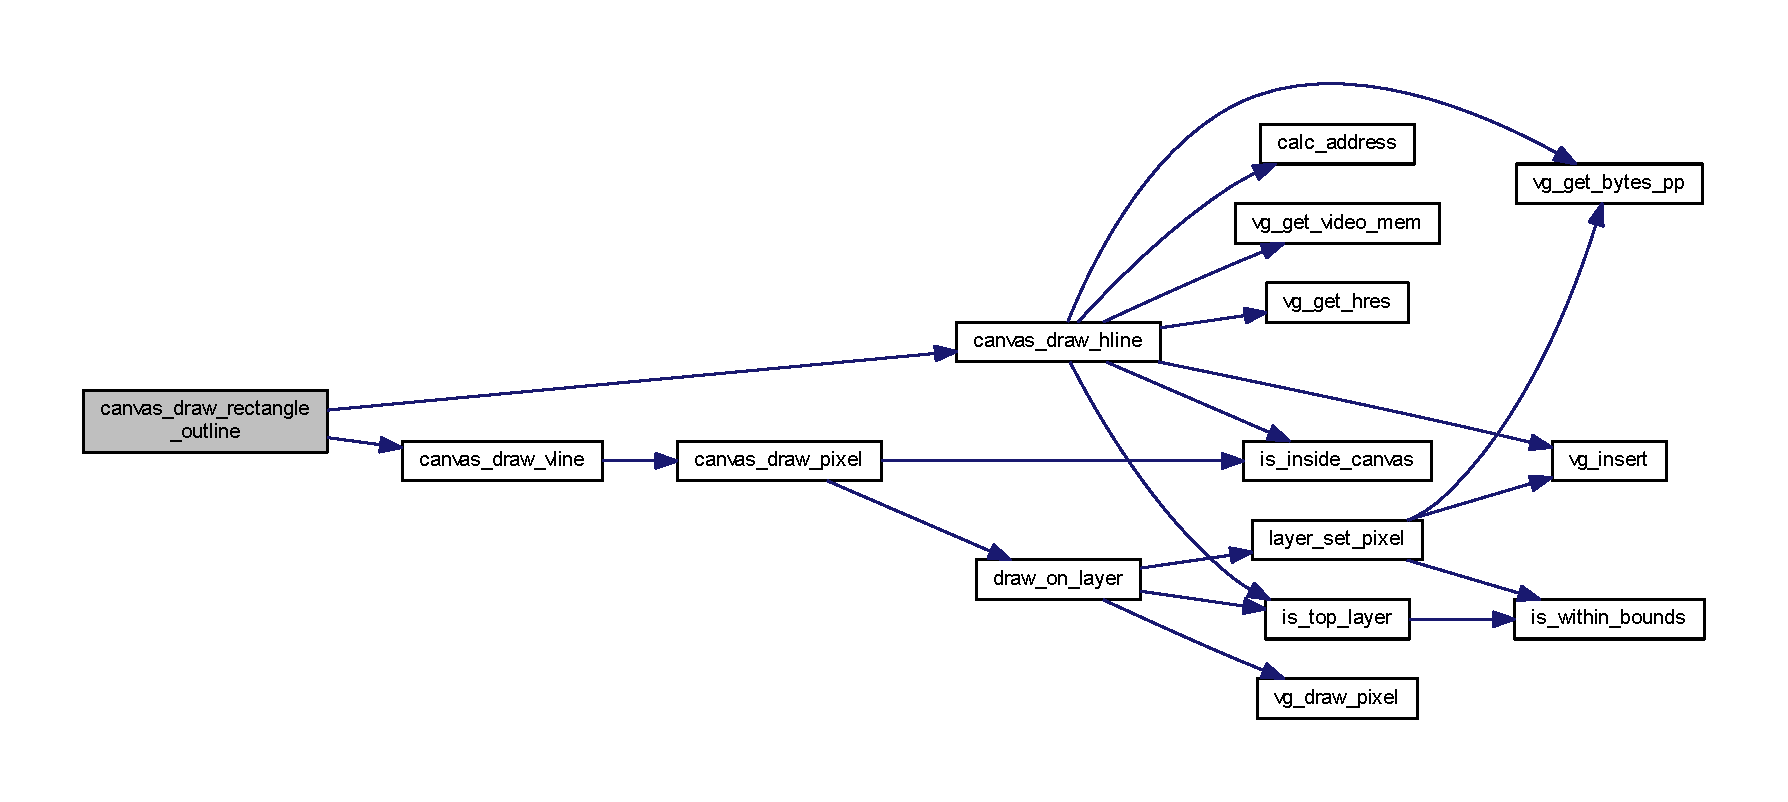
\includegraphics[width=350pt]{group__canvas_ga5301d24065ffd6d68ead836aaeb197f3_cgraph}
\end{center}
\end{figure}
\mbox{\Hypertarget{group__canvas_ga62d3a3d77148b1c1ce74a7fd960601f8}\label{group__canvas_ga62d3a3d77148b1c1ce74a7fd960601f8}} 
\index{canvas@{canvas}!canvas\+\_\+draw\+\_\+shape@{canvas\+\_\+draw\+\_\+shape}}
\index{canvas\+\_\+draw\+\_\+shape@{canvas\+\_\+draw\+\_\+shape}!canvas@{canvas}}
\subsubsection{\texorpdfstring{canvas\+\_\+draw\+\_\+shape()}{canvas\_draw\_shape()}}
{\footnotesize\ttfamily void canvas\+\_\+draw\+\_\+shape (\begin{DoxyParamCaption}\item[{\mbox{\hyperlink{group__canvas_ga55b506070847a13554f8b879c1bfb37c}{Shape}}}]{shape,  }\item[{uint16\+\_\+t}]{click1\+\_\+x,  }\item[{uint16\+\_\+t}]{click1\+\_\+y,  }\item[{uint16\+\_\+t}]{click2\+\_\+x,  }\item[{uint16\+\_\+t}]{click2\+\_\+y,  }\item[{uint32\+\_\+t}]{color,  }\item[{uint16\+\_\+t}]{thickness }\end{DoxyParamCaption})}



Draws a shape on the canvas, based on two mouse clicks. 


\begin{DoxyParams}{Parameters}
{\em shape} & Shape to draw (Enum) \\
\hline
{\em click1\+\_\+x} & X position of the first mouse click \\
\hline
{\em click1\+\_\+y} & Y position of the first mouse click \\
\hline
{\em click2\+\_\+x} & X position of the second mouse click \\
\hline
{\em click2\+\_\+y} & Y position of the second mouse click \\
\hline
{\em color} & Color of the shape \\
\hline
{\em thickness} & Shape thickness (if applied) \\
\hline
\end{DoxyParams}
Here is the call graph for this function\+:\nopagebreak
\begin{figure}[H]
\begin{center}
\leavevmode
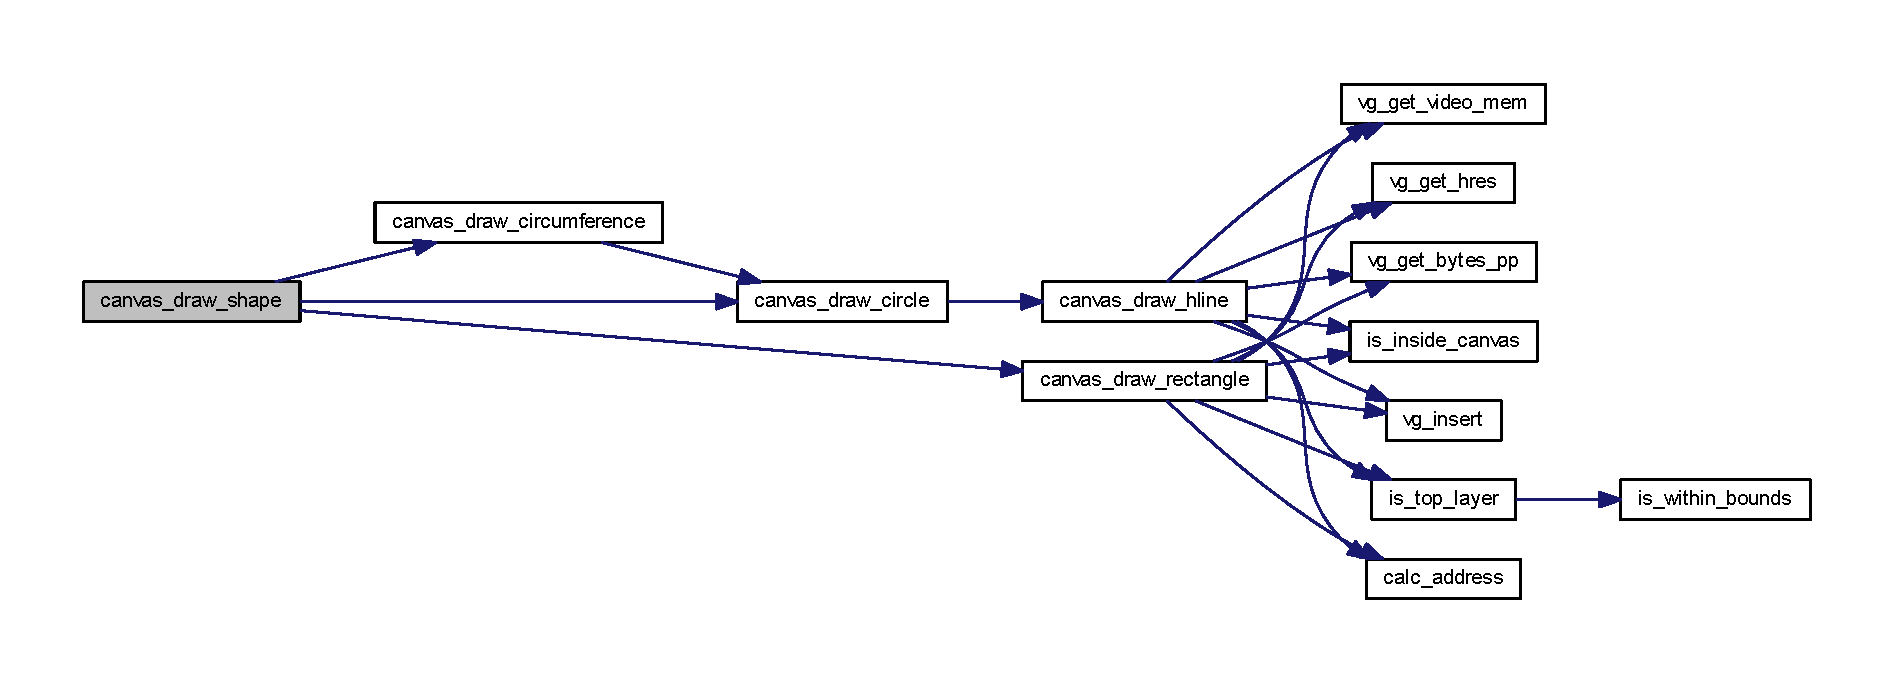
\includegraphics[width=350pt]{group__canvas_ga62d3a3d77148b1c1ce74a7fd960601f8_cgraph}
\end{center}
\end{figure}
Here is the caller graph for this function\+:\nopagebreak
\begin{figure}[H]
\begin{center}
\leavevmode
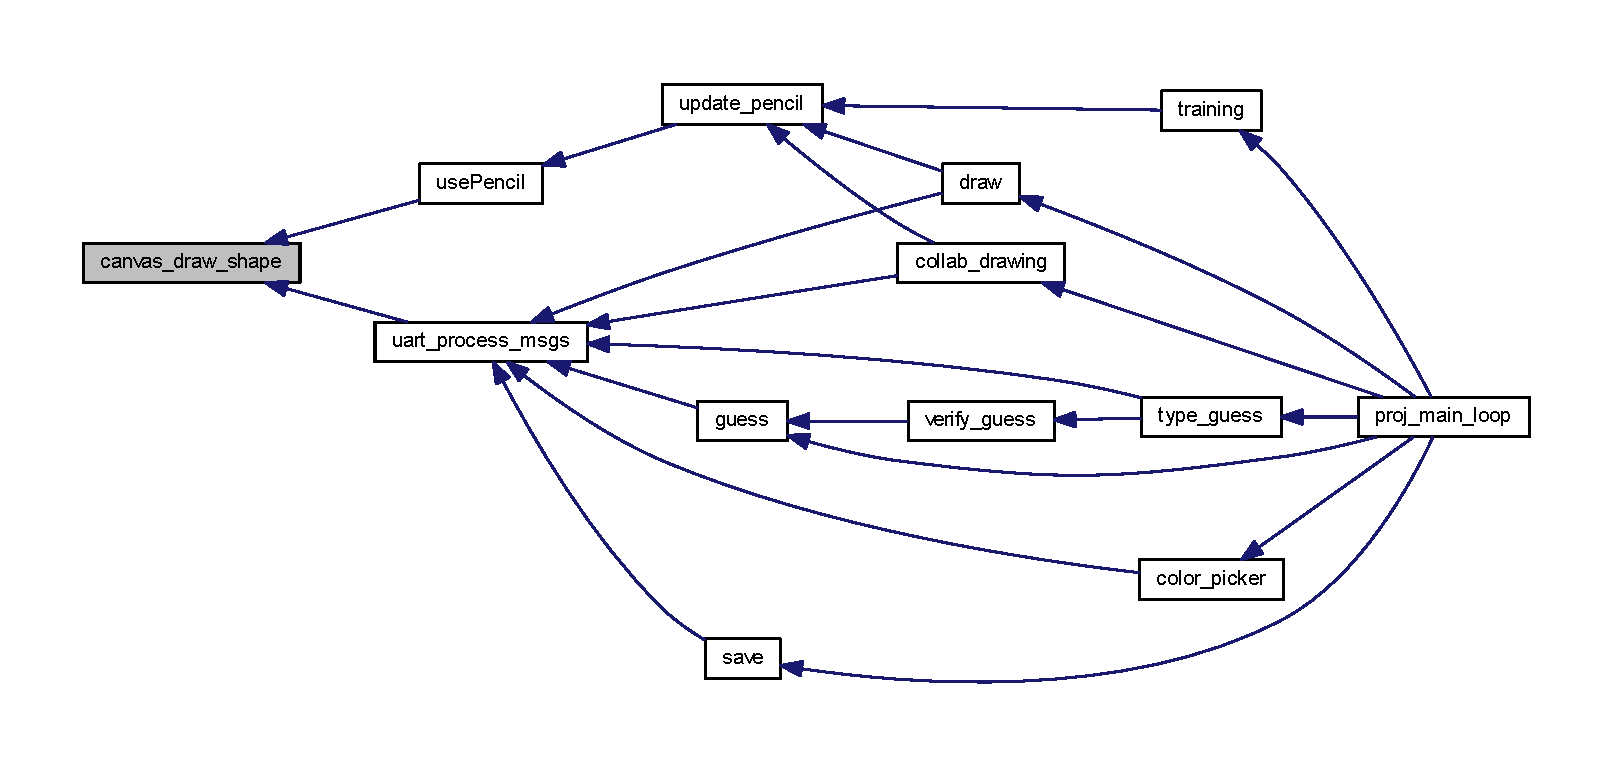
\includegraphics[width=350pt]{group__canvas_ga62d3a3d77148b1c1ce74a7fd960601f8_icgraph}
\end{center}
\end{figure}
\mbox{\Hypertarget{group__canvas_gaa3c801c4663518591f899050db47ad0b}\label{group__canvas_gaa3c801c4663518591f899050db47ad0b}} 
\index{canvas@{canvas}!canvas\+\_\+draw\+\_\+square@{canvas\+\_\+draw\+\_\+square}}
\index{canvas\+\_\+draw\+\_\+square@{canvas\+\_\+draw\+\_\+square}!canvas@{canvas}}
\subsubsection{\texorpdfstring{canvas\+\_\+draw\+\_\+square()}{canvas\_draw\_square()}}
{\footnotesize\ttfamily void canvas\+\_\+draw\+\_\+square (\begin{DoxyParamCaption}\item[{uint16\+\_\+t}]{x,  }\item[{uint16\+\_\+t}]{y,  }\item[{uint16\+\_\+t}]{side\+\_\+len,  }\item[{uint32\+\_\+t}]{color }\end{DoxyParamCaption})}



Draws a square on the canvas. 


\begin{DoxyParams}{Parameters}
{\em x} & X Position of the upper left corner \\
\hline
{\em y} & Y Position of the upper left corner \\
\hline
{\em side\+\_\+len} & Side legth \\
\hline
{\em color} & Square color \\
\hline
\end{DoxyParams}
Here is the call graph for this function\+:\nopagebreak
\begin{figure}[H]
\begin{center}
\leavevmode
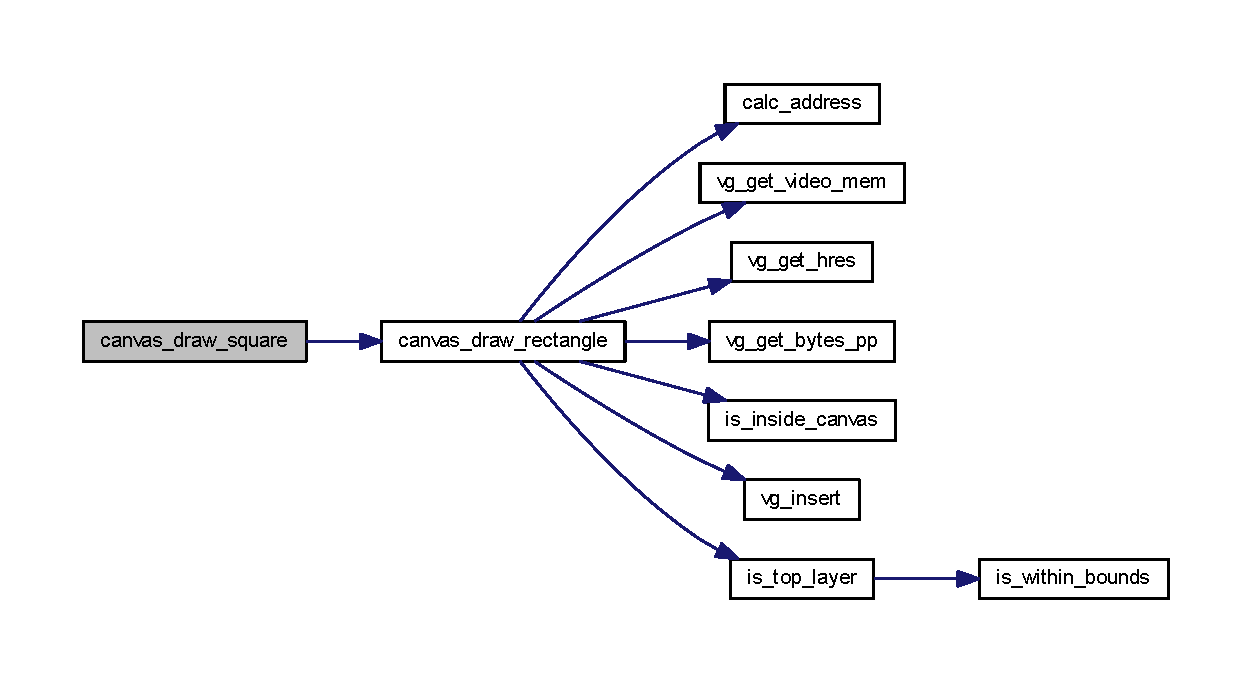
\includegraphics[width=350pt]{group__canvas_gaa3c801c4663518591f899050db47ad0b_cgraph}
\end{center}
\end{figure}
Here is the caller graph for this function\+:\nopagebreak
\begin{figure}[H]
\begin{center}
\leavevmode
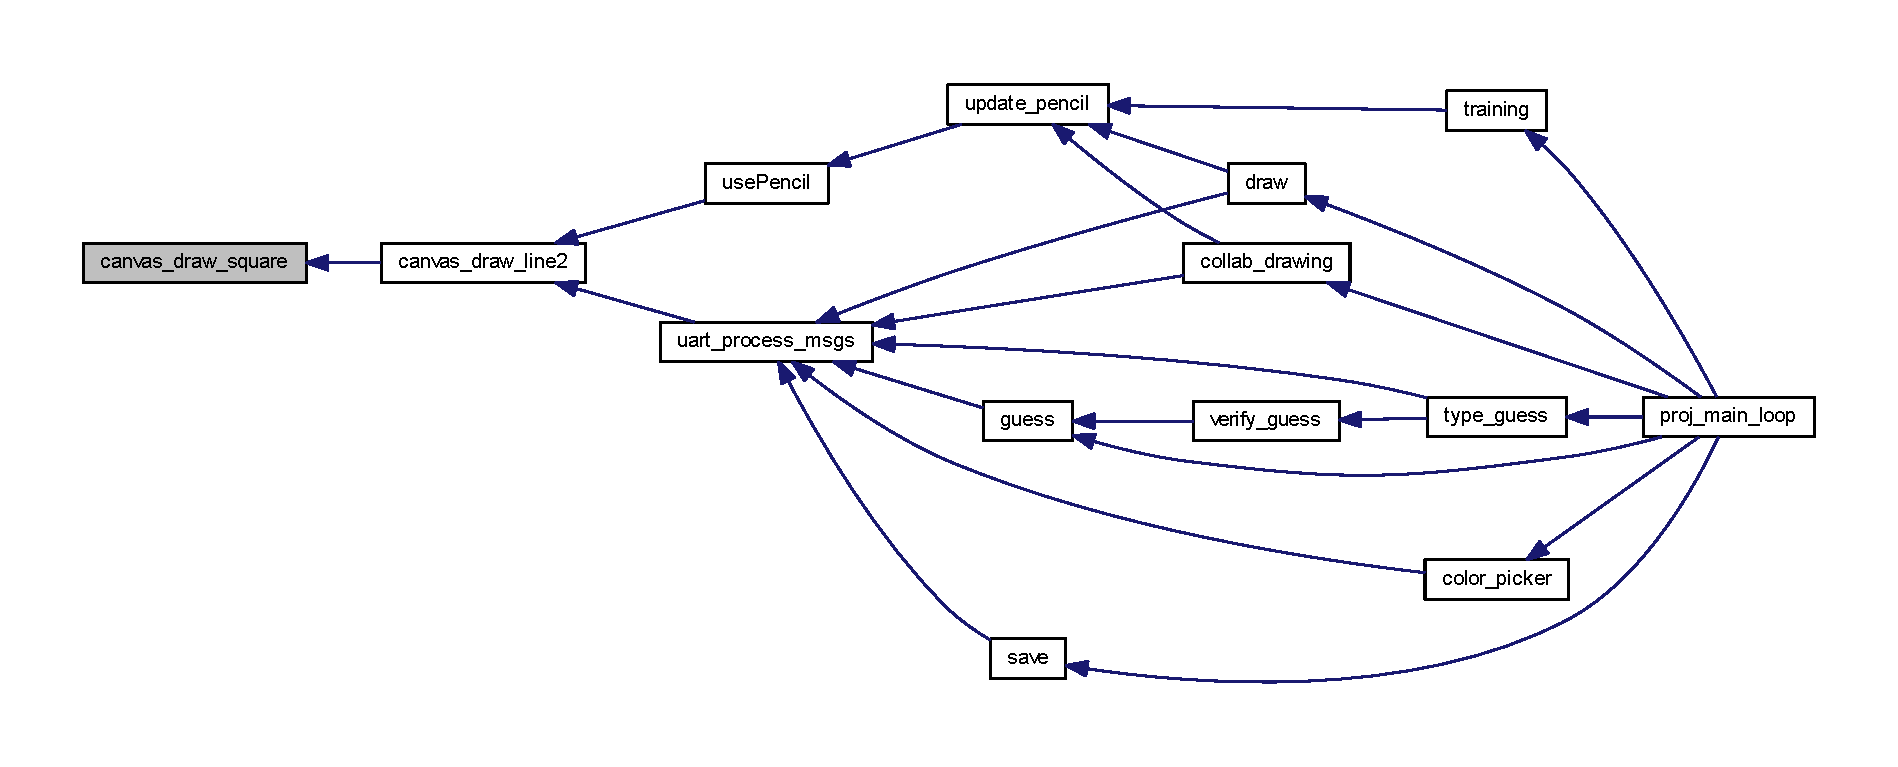
\includegraphics[width=350pt]{group__canvas_gaa3c801c4663518591f899050db47ad0b_icgraph}
\end{center}
\end{figure}
\mbox{\Hypertarget{group__canvas_gae2adf4c3c6c687a5b8885b6a2fa45b3a}\label{group__canvas_gae2adf4c3c6c687a5b8885b6a2fa45b3a}} 
\index{canvas@{canvas}!canvas\+\_\+draw\+\_\+vline@{canvas\+\_\+draw\+\_\+vline}}
\index{canvas\+\_\+draw\+\_\+vline@{canvas\+\_\+draw\+\_\+vline}!canvas@{canvas}}
\subsubsection{\texorpdfstring{canvas\+\_\+draw\+\_\+vline()}{canvas\_draw\_vline()}}
{\footnotesize\ttfamily void canvas\+\_\+draw\+\_\+vline (\begin{DoxyParamCaption}\item[{uint16\+\_\+t}]{x,  }\item[{uint16\+\_\+t}]{y,  }\item[{uint16\+\_\+t}]{len,  }\item[{uint32\+\_\+t}]{color }\end{DoxyParamCaption})}



Draws a vertical line on the canvas. 


\begin{DoxyParams}{Parameters}
{\em x} & X position of the uppermost end \\
\hline
{\em y} & Y position of the uppermost end \\
\hline
{\em len} & Line length \\
\hline
{\em color} & Line color \\
\hline
\end{DoxyParams}
Here is the call graph for this function\+:\nopagebreak
\begin{figure}[H]
\begin{center}
\leavevmode
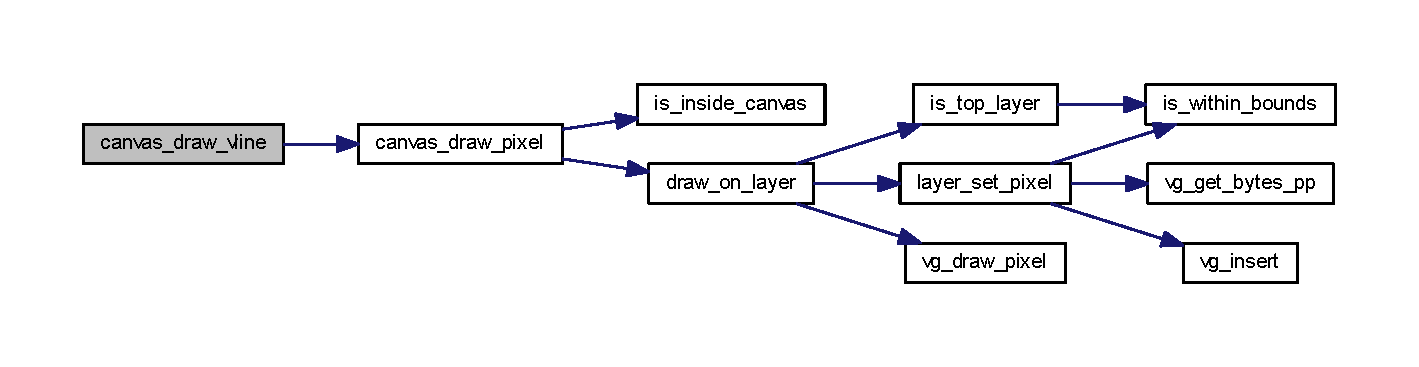
\includegraphics[width=350pt]{group__canvas_gae2adf4c3c6c687a5b8885b6a2fa45b3a_cgraph}
\end{center}
\end{figure}
Here is the caller graph for this function\+:\nopagebreak
\begin{figure}[H]
\begin{center}
\leavevmode
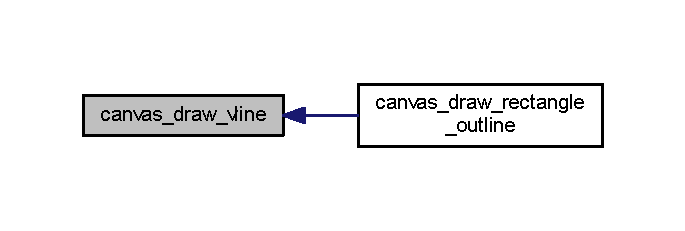
\includegraphics[width=329pt]{group__canvas_gae2adf4c3c6c687a5b8885b6a2fa45b3a_icgraph}
\end{center}
\end{figure}
\mbox{\Hypertarget{group__canvas_gac9eac428cd153893841c96d6a9ce982a}\label{group__canvas_gac9eac428cd153893841c96d6a9ce982a}} 
\index{canvas@{canvas}!canvas\+\_\+get\+\_\+height@{canvas\+\_\+get\+\_\+height}}
\index{canvas\+\_\+get\+\_\+height@{canvas\+\_\+get\+\_\+height}!canvas@{canvas}}
\subsubsection{\texorpdfstring{canvas\+\_\+get\+\_\+height()}{canvas\_get\_height()}}
{\footnotesize\ttfamily int canvas\+\_\+get\+\_\+height (\begin{DoxyParamCaption}{ }\end{DoxyParamCaption})}

\begin{DoxyReturn}{Returns}
int Returns the canvas height. 
\end{DoxyReturn}
Here is the caller graph for this function\+:\nopagebreak
\begin{figure}[H]
\begin{center}
\leavevmode
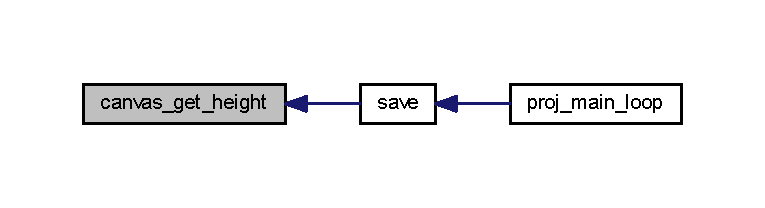
\includegraphics[width=350pt]{group__canvas_gac9eac428cd153893841c96d6a9ce982a_icgraph}
\end{center}
\end{figure}
\mbox{\Hypertarget{group__canvas_gaa7891435582c7691d473ac6532e497a9}\label{group__canvas_gaa7891435582c7691d473ac6532e497a9}} 
\index{canvas@{canvas}!canvas\+\_\+get\+\_\+map@{canvas\+\_\+get\+\_\+map}}
\index{canvas\+\_\+get\+\_\+map@{canvas\+\_\+get\+\_\+map}!canvas@{canvas}}
\subsubsection{\texorpdfstring{canvas\+\_\+get\+\_\+map()}{canvas\_get\_map()}}
{\footnotesize\ttfamily char$\ast$ canvas\+\_\+get\+\_\+map (\begin{DoxyParamCaption}{ }\end{DoxyParamCaption})}

\begin{DoxyReturn}{Returns}
char$\ast$ Returns a pixel map of the canvas. (allocated memory) 
\end{DoxyReturn}
Here is the call graph for this function\+:\nopagebreak
\begin{figure}[H]
\begin{center}
\leavevmode
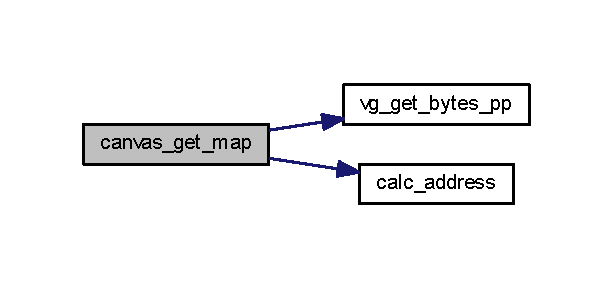
\includegraphics[width=294pt]{group__canvas_gaa7891435582c7691d473ac6532e497a9_cgraph}
\end{center}
\end{figure}
Here is the caller graph for this function\+:\nopagebreak
\begin{figure}[H]
\begin{center}
\leavevmode
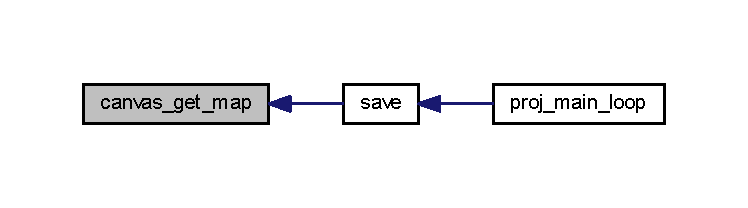
\includegraphics[width=350pt]{group__canvas_gaa7891435582c7691d473ac6532e497a9_icgraph}
\end{center}
\end{figure}
\mbox{\Hypertarget{group__canvas_gaa5703f24ea2a8ec8bee2c73225c39553}\label{group__canvas_gaa5703f24ea2a8ec8bee2c73225c39553}} 
\index{canvas@{canvas}!canvas\+\_\+get\+\_\+width@{canvas\+\_\+get\+\_\+width}}
\index{canvas\+\_\+get\+\_\+width@{canvas\+\_\+get\+\_\+width}!canvas@{canvas}}
\subsubsection{\texorpdfstring{canvas\+\_\+get\+\_\+width()}{canvas\_get\_width()}}
{\footnotesize\ttfamily int canvas\+\_\+get\+\_\+width (\begin{DoxyParamCaption}{ }\end{DoxyParamCaption})}

\begin{DoxyReturn}{Returns}
int Returns the canvas width. 
\end{DoxyReturn}
Here is the caller graph for this function\+:\nopagebreak
\begin{figure}[H]
\begin{center}
\leavevmode
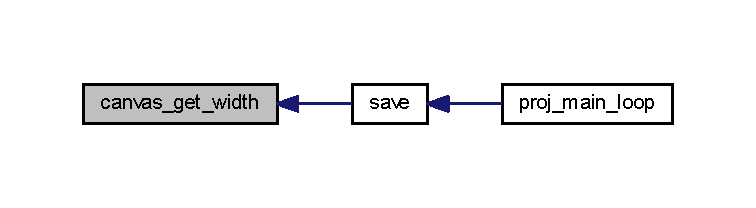
\includegraphics[width=350pt]{group__canvas_gaa5703f24ea2a8ec8bee2c73225c39553_icgraph}
\end{center}
\end{figure}
\mbox{\Hypertarget{group__canvas_ga3c9ed75a75ae36bc6fc7591952fccf17}\label{group__canvas_ga3c9ed75a75ae36bc6fc7591952fccf17}} 
\index{canvas@{canvas}!canvas\+\_\+save\+\_\+drawing@{canvas\+\_\+save\+\_\+drawing}}
\index{canvas\+\_\+save\+\_\+drawing@{canvas\+\_\+save\+\_\+drawing}!canvas@{canvas}}
\subsubsection{\texorpdfstring{canvas\+\_\+save\+\_\+drawing()}{canvas\_save\_drawing()}}
{\footnotesize\ttfamily void canvas\+\_\+save\+\_\+drawing (\begin{DoxyParamCaption}{ }\end{DoxyParamCaption})}



Stores the current canvas pixel map in a buffer (for the next undo action). Sets an internal is\+Drawing flag. 

Here is the call graph for this function\+:\nopagebreak
\begin{figure}[H]
\begin{center}
\leavevmode
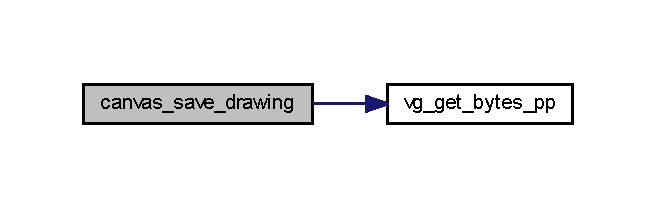
\includegraphics[width=315pt]{group__canvas_ga3c9ed75a75ae36bc6fc7591952fccf17_cgraph}
\end{center}
\end{figure}
Here is the caller graph for this function\+:\nopagebreak
\begin{figure}[H]
\begin{center}
\leavevmode
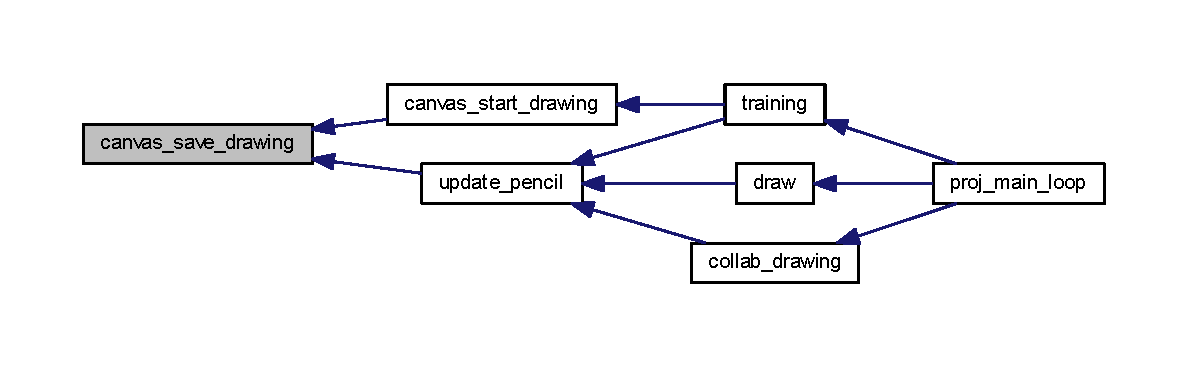
\includegraphics[width=350pt]{group__canvas_ga3c9ed75a75ae36bc6fc7591952fccf17_icgraph}
\end{center}
\end{figure}
\mbox{\Hypertarget{group__canvas_ga82c276340112469fe11a819ade81ead2}\label{group__canvas_ga82c276340112469fe11a819ade81ead2}} 
\index{canvas@{canvas}!canvas\+\_\+set\+\_\+color@{canvas\+\_\+set\+\_\+color}}
\index{canvas\+\_\+set\+\_\+color@{canvas\+\_\+set\+\_\+color}!canvas@{canvas}}
\subsubsection{\texorpdfstring{canvas\+\_\+set\+\_\+color()}{canvas\_set\_color()}}
{\footnotesize\ttfamily void canvas\+\_\+set\+\_\+color (\begin{DoxyParamCaption}\item[{uint32\+\_\+t}]{color }\end{DoxyParamCaption})}



Sets the canvas color, filling it. 


\begin{DoxyParams}{Parameters}
{\em color} & Color to fill with \\
\hline
\end{DoxyParams}
Here is the call graph for this function\+:\nopagebreak
\begin{figure}[H]
\begin{center}
\leavevmode
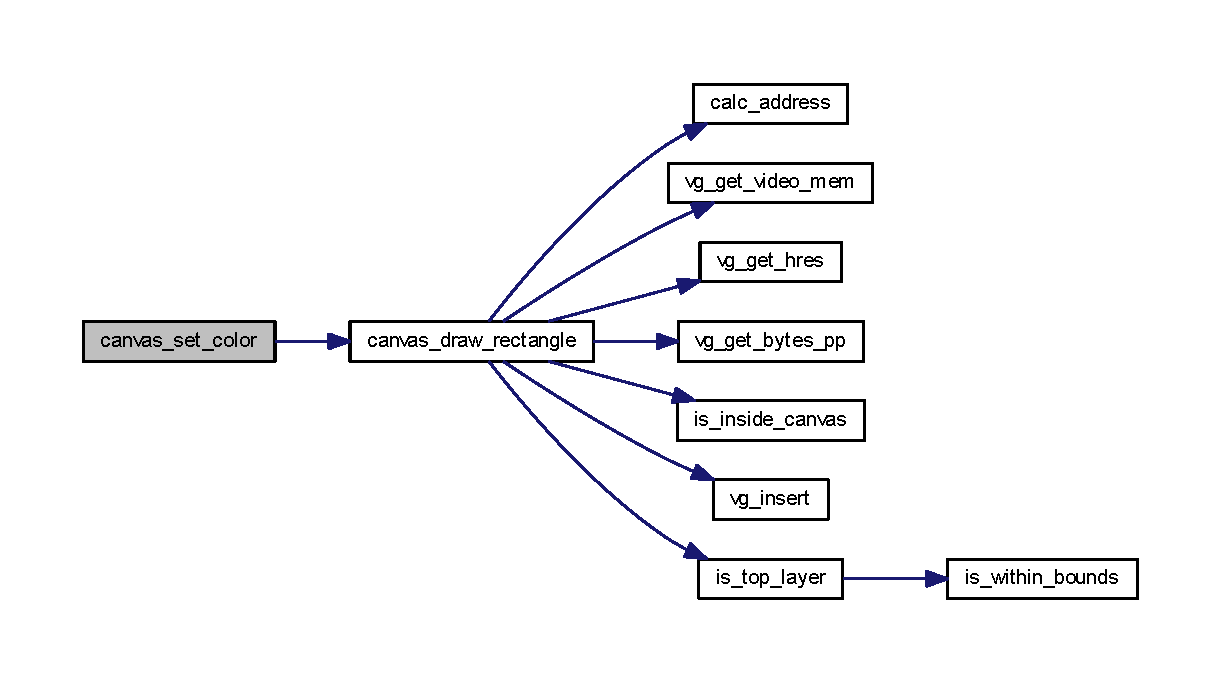
\includegraphics[width=350pt]{group__canvas_ga82c276340112469fe11a819ade81ead2_cgraph}
\end{center}
\end{figure}
Here is the caller graph for this function\+:\nopagebreak
\begin{figure}[H]
\begin{center}
\leavevmode
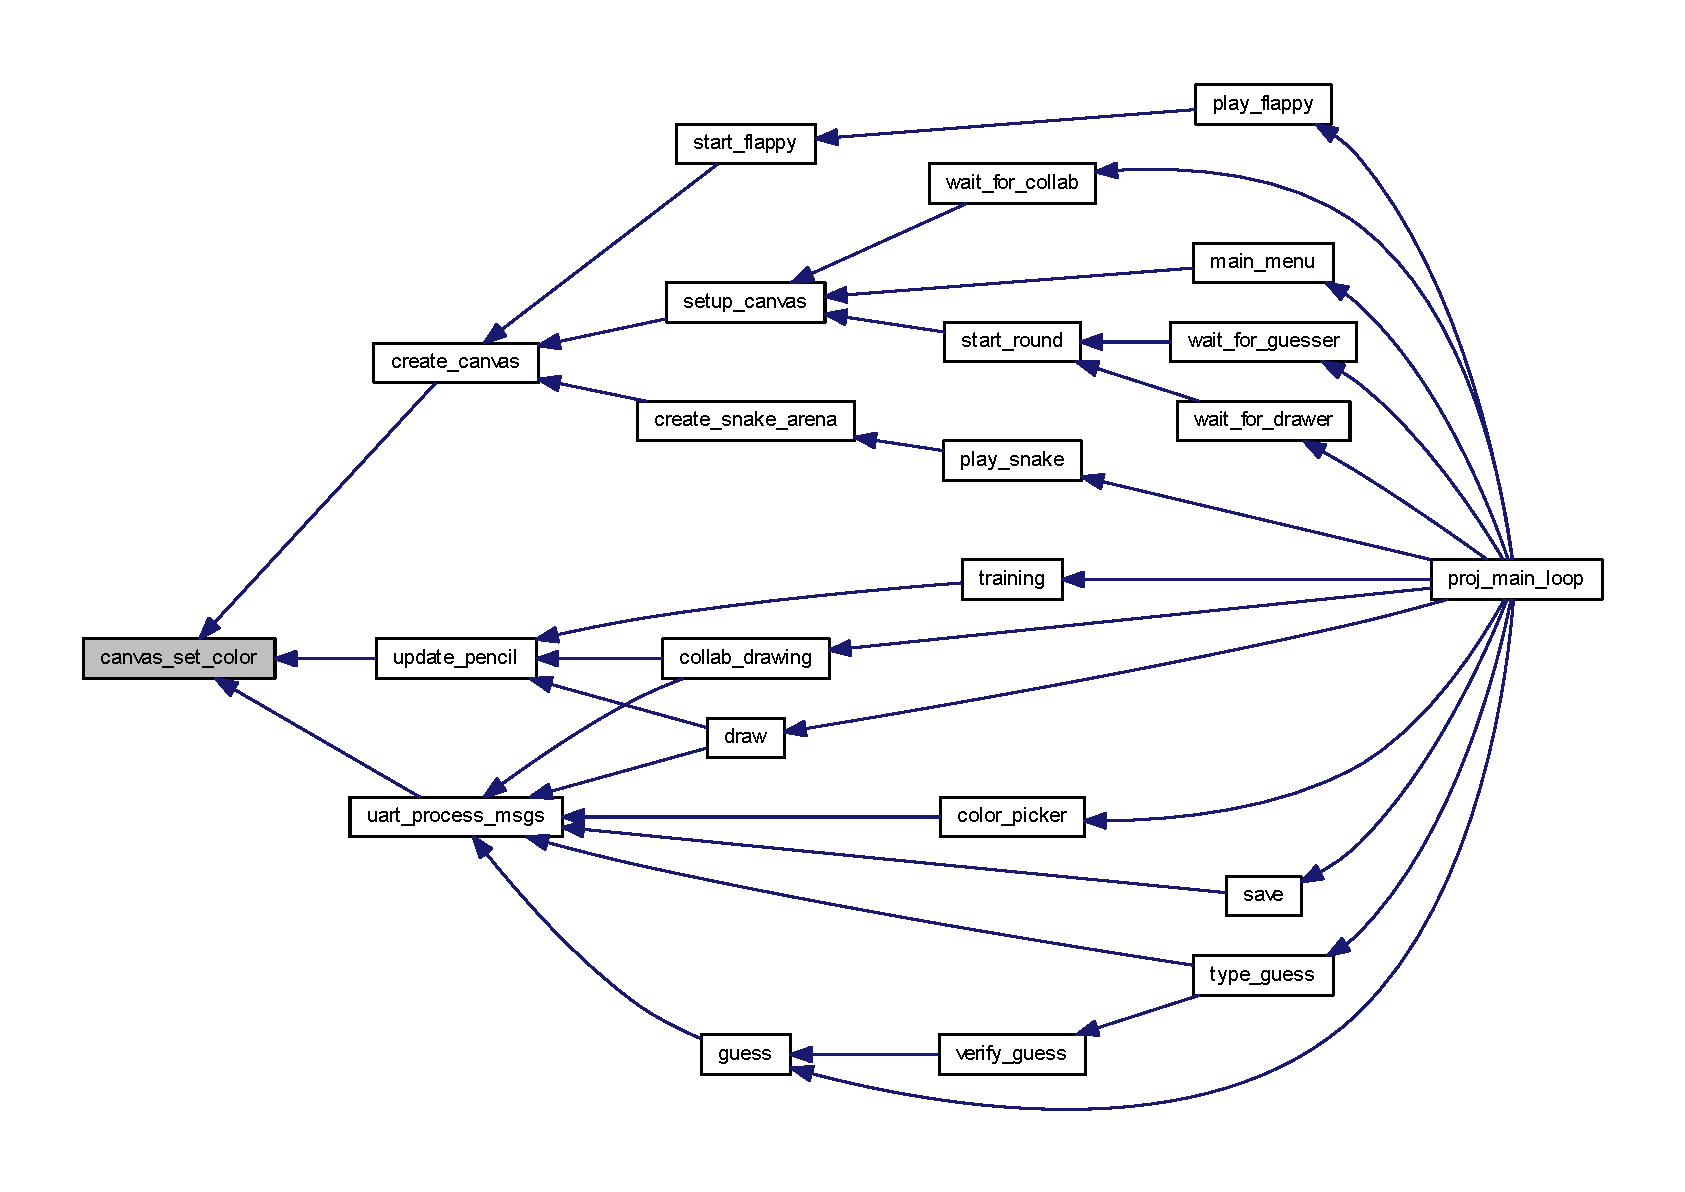
\includegraphics[width=350pt]{group__canvas_ga82c276340112469fe11a819ade81ead2_icgraph}
\end{center}
\end{figure}
\mbox{\Hypertarget{group__canvas_ga042599a460db7bc889fdf51cb56ae732}\label{group__canvas_ga042599a460db7bc889fdf51cb56ae732}} 
\index{canvas@{canvas}!canvas\+\_\+set\+\_\+outline@{canvas\+\_\+set\+\_\+outline}}
\index{canvas\+\_\+set\+\_\+outline@{canvas\+\_\+set\+\_\+outline}!canvas@{canvas}}
\subsubsection{\texorpdfstring{canvas\+\_\+set\+\_\+outline()}{canvas\_set\_outline()}}
{\footnotesize\ttfamily void canvas\+\_\+set\+\_\+outline (\begin{DoxyParamCaption}\item[{uint32\+\_\+t}]{color }\end{DoxyParamCaption})}



Sets the canvas outline (thickness 5) 


\begin{DoxyParams}{Parameters}
{\em color} & Color to draw the outline with \\
\hline
\end{DoxyParams}
Here is the call graph for this function\+:\nopagebreak
\begin{figure}[H]
\begin{center}
\leavevmode
\includegraphics[width=350pt]{group__canvas_ga042599a460db7bc889fdf51cb56ae732_cgraph}
\end{center}
\end{figure}
Here is the caller graph for this function\+:\nopagebreak
\begin{figure}[H]
\begin{center}
\leavevmode
\includegraphics[width=350pt]{group__canvas_ga042599a460db7bc889fdf51cb56ae732_icgraph}
\end{center}
\end{figure}
\mbox{\Hypertarget{group__canvas_ga3a6a181542db6b70c3aadc411073943d}\label{group__canvas_ga3a6a181542db6b70c3aadc411073943d}} 
\index{canvas@{canvas}!canvas\+\_\+start\+\_\+drawing@{canvas\+\_\+start\+\_\+drawing}}
\index{canvas\+\_\+start\+\_\+drawing@{canvas\+\_\+start\+\_\+drawing}!canvas@{canvas}}
\subsubsection{\texorpdfstring{canvas\+\_\+start\+\_\+drawing()}{canvas\_start\_drawing()}}
{\footnotesize\ttfamily void canvas\+\_\+start\+\_\+drawing (\begin{DoxyParamCaption}\item[{uint16\+\_\+t}]{x,  }\item[{uint16\+\_\+t}]{y }\end{DoxyParamCaption})}



Saves drawing for the next undo action, only if the cursor position is inside the canvas and the is\+Drawing flag is not set. 


\begin{DoxyParams}{Parameters}
{\em x} & X position of the cursor \\
\hline
{\em y} & Y position of the cursor \\
\hline
\end{DoxyParams}
Here is the call graph for this function\+:\nopagebreak
\begin{figure}[H]
\begin{center}
\leavevmode
\includegraphics[width=350pt]{group__canvas_ga3a6a181542db6b70c3aadc411073943d_cgraph}
\end{center}
\end{figure}
Here is the caller graph for this function\+:\nopagebreak
\begin{figure}[H]
\begin{center}
\leavevmode
\includegraphics[width=350pt]{group__canvas_ga3a6a181542db6b70c3aadc411073943d_icgraph}
\end{center}
\end{figure}
\mbox{\Hypertarget{group__canvas_ga95994c1c125e70ef4d9380e80ed9c3ab}\label{group__canvas_ga95994c1c125e70ef4d9380e80ed9c3ab}} 
\index{canvas@{canvas}!canvas\+\_\+stop\+\_\+drawing@{canvas\+\_\+stop\+\_\+drawing}}
\index{canvas\+\_\+stop\+\_\+drawing@{canvas\+\_\+stop\+\_\+drawing}!canvas@{canvas}}
\subsubsection{\texorpdfstring{canvas\+\_\+stop\+\_\+drawing()}{canvas\_stop\_drawing()}}
{\footnotesize\ttfamily void canvas\+\_\+stop\+\_\+drawing (\begin{DoxyParamCaption}{ }\end{DoxyParamCaption})}



Unsets the is\+Drawing flag. 

Here is the caller graph for this function\+:\nopagebreak
\begin{figure}[H]
\begin{center}
\leavevmode
\includegraphics[width=350pt]{group__canvas_ga95994c1c125e70ef4d9380e80ed9c3ab_icgraph}
\end{center}
\end{figure}
\mbox{\Hypertarget{group__canvas_ga96be607ebdf4fda25a050f017d68db93}\label{group__canvas_ga96be607ebdf4fda25a050f017d68db93}} 
\index{canvas@{canvas}!canvas\+\_\+undo@{canvas\+\_\+undo}}
\index{canvas\+\_\+undo@{canvas\+\_\+undo}!canvas@{canvas}}
\subsubsection{\texorpdfstring{canvas\+\_\+undo()}{canvas\_undo()}}
{\footnotesize\ttfamily void canvas\+\_\+undo (\begin{DoxyParamCaption}{ }\end{DoxyParamCaption})}



Edits the canvas to the last saved pixel map. 

Here is the call graph for this function\+:\nopagebreak
\begin{figure}[H]
\begin{center}
\leavevmode
\includegraphics[width=350pt]{group__canvas_ga96be607ebdf4fda25a050f017d68db93_cgraph}
\end{center}
\end{figure}
Here is the caller graph for this function\+:\nopagebreak
\begin{figure}[H]
\begin{center}
\leavevmode
\includegraphics[width=350pt]{group__canvas_ga96be607ebdf4fda25a050f017d68db93_icgraph}
\end{center}
\end{figure}
\mbox{\Hypertarget{group__canvas_gab462a38a3f3a612931c008e28e816a8d}\label{group__canvas_gab462a38a3f3a612931c008e28e816a8d}} 
\index{canvas@{canvas}!canvas\+\_\+update@{canvas\+\_\+update}}
\index{canvas\+\_\+update@{canvas\+\_\+update}!canvas@{canvas}}
\subsubsection{\texorpdfstring{canvas\+\_\+update()}{canvas\_update()}}
{\footnotesize\ttfamily void canvas\+\_\+update (\begin{DoxyParamCaption}{ }\end{DoxyParamCaption})}



Updates the canvas with its layer contents. 

Here is the call graph for this function\+:\nopagebreak
\begin{figure}[H]
\begin{center}
\leavevmode
\includegraphics[width=350pt]{group__canvas_gab462a38a3f3a612931c008e28e816a8d_cgraph}
\end{center}
\end{figure}
Here is the caller graph for this function\+:\nopagebreak
\begin{figure}[H]
\begin{center}
\leavevmode
\includegraphics[width=350pt]{group__canvas_gab462a38a3f3a612931c008e28e816a8d_icgraph}
\end{center}
\end{figure}
\mbox{\Hypertarget{group__canvas_ga8ca57c812327763152c635d235e3104e}\label{group__canvas_ga8ca57c812327763152c635d235e3104e}} 
\index{canvas@{canvas}!create\+\_\+canvas@{create\+\_\+canvas}}
\index{create\+\_\+canvas@{create\+\_\+canvas}!canvas@{canvas}}
\subsubsection{\texorpdfstring{create\+\_\+canvas()}{create\_canvas()}}
{\footnotesize\ttfamily void create\+\_\+canvas (\begin{DoxyParamCaption}\item[{\mbox{\hyperlink{struct_layer}{Layer}} $\ast$}]{layer,  }\item[{uint16\+\_\+t}]{x\+Min,  }\item[{uint16\+\_\+t}]{y\+Min,  }\item[{uint16\+\_\+t}]{x\+Max,  }\item[{uint16\+\_\+t}]{y\+Max,  }\item[{uint32\+\_\+t}]{color }\end{DoxyParamCaption})}



Creates a canvas and draws it on the screen, with a black outline. 


\begin{DoxyParams}{Parameters}
{\em layer} & \mbox{\hyperlink{struct_layer}{Layer}} to draw the canvas on. \\
\hline
{\em x\+Min} & X position of the upper left corner. \\
\hline
{\em y\+Min} & Y position of the upper left corner. \\
\hline
{\em x\+Max} & X position of the lower right corner. \\
\hline
{\em y\+Max} & Y position of the lower right corner. \\
\hline
{\em color} & Color to fill the canvas with \\
\hline
\end{DoxyParams}
Here is the call graph for this function\+:\nopagebreak
\begin{figure}[H]
\begin{center}
\leavevmode
\includegraphics[width=350pt]{group__canvas_ga8ca57c812327763152c635d235e3104e_cgraph}
\end{center}
\end{figure}
Here is the caller graph for this function\+:\nopagebreak
\begin{figure}[H]
\begin{center}
\leavevmode
\includegraphics[width=350pt]{group__canvas_ga8ca57c812327763152c635d235e3104e_icgraph}
\end{center}
\end{figure}
\mbox{\Hypertarget{group__canvas_ga1574bd14271b62f79a866c5b961ea41a}\label{group__canvas_ga1574bd14271b62f79a866c5b961ea41a}} 
\index{canvas@{canvas}!destroy\+\_\+canvas@{destroy\+\_\+canvas}}
\index{destroy\+\_\+canvas@{destroy\+\_\+canvas}!canvas@{canvas}}
\subsubsection{\texorpdfstring{destroy\+\_\+canvas()}{destroy\_canvas()}}
{\footnotesize\ttfamily void destroy\+\_\+canvas (\begin{DoxyParamCaption}{ }\end{DoxyParamCaption})}



Frees the memory used by the canvas, so that a new one can be created later. 

Here is the caller graph for this function\+:\nopagebreak
\begin{figure}[H]
\begin{center}
\leavevmode
\includegraphics[width=350pt]{group__canvas_ga1574bd14271b62f79a866c5b961ea41a_icgraph}
\end{center}
\end{figure}
\mbox{\Hypertarget{group__canvas_ga85fca0492c1f7ec8e1d20a9b5e48be1c}\label{group__canvas_ga85fca0492c1f7ec8e1d20a9b5e48be1c}} 
\index{canvas@{canvas}!is\+\_\+inside\+\_\+canvas@{is\+\_\+inside\+\_\+canvas}}
\index{is\+\_\+inside\+\_\+canvas@{is\+\_\+inside\+\_\+canvas}!canvas@{canvas}}
\subsubsection{\texorpdfstring{is\+\_\+inside\+\_\+canvas()}{is\_inside\_canvas()}}
{\footnotesize\ttfamily bool is\+\_\+inside\+\_\+canvas (\begin{DoxyParamCaption}\item[{uint16\+\_\+t}]{x,  }\item[{uint16\+\_\+t}]{y }\end{DoxyParamCaption})}



Checks if a position is inside the canvas. 


\begin{DoxyParams}{Parameters}
{\em x} & X position to check \\
\hline
{\em y} & Y position to check \\
\hline
\end{DoxyParams}
\begin{DoxyReturn}{Returns}
true The position is inside the canvas 

false The position is outside the canvas 
\end{DoxyReturn}
Here is the caller graph for this function\+:\nopagebreak
\begin{figure}[H]
\begin{center}
\leavevmode
\includegraphics[width=350pt]{group__canvas_ga85fca0492c1f7ec8e1d20a9b5e48be1c_icgraph}
\end{center}
\end{figure}
\mbox{\Hypertarget{group__canvas_ga4bac68c651bfc3551d7f9fbbdf7d0e18}\label{group__canvas_ga4bac68c651bfc3551d7f9fbbdf7d0e18}} 
\index{canvas@{canvas}!rainbow@{rainbow}}
\index{rainbow@{rainbow}!canvas@{canvas}}
\subsubsection{\texorpdfstring{rainbow()}{rainbow()}}
{\footnotesize\ttfamily uint32\+\_\+t rainbow (\begin{DoxyParamCaption}\item[{uint32\+\_\+t}]{old\+\_\+color }\end{DoxyParamCaption})}



Following a rainbow gradient, gets the next color in the gradient. 


\begin{DoxyParams}{Parameters}
{\em old\+\_\+color} & Previous color \\
\hline
\end{DoxyParams}
\begin{DoxyReturn}{Returns}
uint32\+\_\+t Returns the following color. 
\end{DoxyReturn}
Here is the call graph for this function\+:\nopagebreak
\begin{figure}[H]
\begin{center}
\leavevmode
\includegraphics[width=273pt]{group__canvas_ga4bac68c651bfc3551d7f9fbbdf7d0e18_cgraph}
\end{center}
\end{figure}
Here is the caller graph for this function\+:\nopagebreak
\begin{figure}[H]
\begin{center}
\leavevmode
\includegraphics[width=350pt]{group__canvas_ga4bac68c651bfc3551d7f9fbbdf7d0e18_icgraph}
\end{center}
\end{figure}


\subsection{Variable Documentation}
\mbox{\Hypertarget{group__canvas_ga438a71c178c014aef3de261dbc7b483e}\label{group__canvas_ga438a71c178c014aef3de261dbc7b483e}} 
\index{canvas@{canvas}!height@{height}}
\index{height@{height}!canvas@{canvas}}
\subsubsection{\texorpdfstring{height}{height}}
{\footnotesize\ttfamily uint16\+\_\+t Canvas\+::height}



\mbox{\hyperlink{struct_canvas}{Canvas}} height (redundant) 

\mbox{\Hypertarget{group__canvas_gaf72f42e64c0a72256001acc241f287ce}\label{group__canvas_gaf72f42e64c0a72256001acc241f287ce}} 
\index{canvas@{canvas}!layer@{layer}}
\index{layer@{layer}!canvas@{canvas}}
\subsubsection{\texorpdfstring{layer}{layer}}
{\footnotesize\ttfamily \mbox{\hyperlink{struct_layer}{Layer}}$\ast$ Canvas\+::layer}



\mbox{\hyperlink{struct_layer}{Layer}} to draw the canvas on. 

\mbox{\Hypertarget{group__canvas_gaee9a970b56d8660b35047a170abc58ca}\label{group__canvas_gaee9a970b56d8660b35047a170abc58ca}} 
\index{canvas@{canvas}!width@{width}}
\index{width@{width}!canvas@{canvas}}
\subsubsection{\texorpdfstring{width}{width}}
{\footnotesize\ttfamily uint16\+\_\+t Canvas\+::width}



\mbox{\hyperlink{struct_canvas}{Canvas}} width (redundant) 

\mbox{\Hypertarget{group__canvas_ga423c26269827a5beb80f569ba8076ae2}\label{group__canvas_ga423c26269827a5beb80f569ba8076ae2}} 
\index{canvas@{canvas}!x\+Max@{x\+Max}}
\index{x\+Max@{x\+Max}!canvas@{canvas}}
\subsubsection{\texorpdfstring{x\+Max}{xMax}}
{\footnotesize\ttfamily uint16\+\_\+t Canvas\+::x\+Max}

\mbox{\Hypertarget{group__canvas_ga10925446227a312ac91f903acaf074e8}\label{group__canvas_ga10925446227a312ac91f903acaf074e8}} 
\index{canvas@{canvas}!x\+Min@{x\+Min}}
\index{x\+Min@{x\+Min}!canvas@{canvas}}
\subsubsection{\texorpdfstring{x\+Min}{xMin}}
{\footnotesize\ttfamily uint16\+\_\+t Canvas\+::x\+Min}

\mbox{\Hypertarget{group__canvas_ga2990194f0baef3d23cb75299cc39987d}\label{group__canvas_ga2990194f0baef3d23cb75299cc39987d}} 
\index{canvas@{canvas}!y\+Max@{y\+Max}}
\index{y\+Max@{y\+Max}!canvas@{canvas}}
\subsubsection{\texorpdfstring{y\+Max}{yMax}}
{\footnotesize\ttfamily uint16\+\_\+t Canvas\+::y\+Max}



Position of the lower right corner. 

\mbox{\Hypertarget{group__canvas_ga91a71d5f9030202359d000a5fb54423a}\label{group__canvas_ga91a71d5f9030202359d000a5fb54423a}} 
\index{canvas@{canvas}!y\+Min@{y\+Min}}
\index{y\+Min@{y\+Min}!canvas@{canvas}}
\subsubsection{\texorpdfstring{y\+Min}{yMin}}
{\footnotesize\ttfamily uint16\+\_\+t Canvas\+::y\+Min}



Position of the upper left corner. 


\hypertarget{group__clock}{}\section{clock}
\label{group__clock}\index{clock@{clock}}
\subsection*{Functions}
\begin{DoxyCompactItemize}
\item 
void \mbox{\hyperlink{group__clock_ga59029f76a2cbf7aad54d01f50cf80cf9}{create\+\_\+big\+\_\+ben}} ()
\begin{DoxyCompactList}\small\item\em Creates a big clock on the top left of the screen, displaying the current date. \end{DoxyCompactList}\item 
void \mbox{\hyperlink{group__clock_ga74cbf0ece67234028fdd0465d51bfc0d}{destroy\+\_\+big\+\_\+ben}} ()
\begin{DoxyCompactList}\small\item\em Destroys the big clock. \end{DoxyCompactList}\item 
void \mbox{\hyperlink{group__clock_gac56b75476d51e272a9efcbb174ed7bf8}{update\+\_\+big\+\_\+ben}} (bool force)
\begin{DoxyCompactList}\small\item\em Updates the clock on the screen with the current date. \end{DoxyCompactList}\end{DoxyCompactItemize}


\subsection{Detailed Description}
Functions used to create and update a date-\/displaying clock 

\subsection{Function Documentation}
\mbox{\Hypertarget{group__clock_ga59029f76a2cbf7aad54d01f50cf80cf9}\label{group__clock_ga59029f76a2cbf7aad54d01f50cf80cf9}} 
\index{clock@{clock}!create\+\_\+big\+\_\+ben@{create\+\_\+big\+\_\+ben}}
\index{create\+\_\+big\+\_\+ben@{create\+\_\+big\+\_\+ben}!clock@{clock}}
\subsubsection{\texorpdfstring{create\+\_\+big\+\_\+ben()}{create\_big\_ben()}}
{\footnotesize\ttfamily void create\+\_\+big\+\_\+ben (\begin{DoxyParamCaption}{ }\end{DoxyParamCaption})}



Creates a big clock on the top left of the screen, displaying the current date. 

Here is the call graph for this function\+:
\nopagebreak
\begin{figure}[H]
\begin{center}
\leavevmode
\includegraphics[width=350pt]{group__clock_ga59029f76a2cbf7aad54d01f50cf80cf9_cgraph}
\end{center}
\end{figure}
Here is the caller graph for this function\+:\nopagebreak
\begin{figure}[H]
\begin{center}
\leavevmode
\includegraphics[width=350pt]{group__clock_ga59029f76a2cbf7aad54d01f50cf80cf9_icgraph}
\end{center}
\end{figure}
\mbox{\Hypertarget{group__clock_ga74cbf0ece67234028fdd0465d51bfc0d}\label{group__clock_ga74cbf0ece67234028fdd0465d51bfc0d}} 
\index{clock@{clock}!destroy\+\_\+big\+\_\+ben@{destroy\+\_\+big\+\_\+ben}}
\index{destroy\+\_\+big\+\_\+ben@{destroy\+\_\+big\+\_\+ben}!clock@{clock}}
\subsubsection{\texorpdfstring{destroy\+\_\+big\+\_\+ben()}{destroy\_big\_ben()}}
{\footnotesize\ttfamily void destroy\+\_\+big\+\_\+ben (\begin{DoxyParamCaption}{ }\end{DoxyParamCaption})}



Destroys the big clock. 

Here is the call graph for this function\+:\nopagebreak
\begin{figure}[H]
\begin{center}
\leavevmode
\includegraphics[width=350pt]{group__clock_ga74cbf0ece67234028fdd0465d51bfc0d_cgraph}
\end{center}
\end{figure}
Here is the caller graph for this function\+:\nopagebreak
\begin{figure}[H]
\begin{center}
\leavevmode
\includegraphics[width=350pt]{group__clock_ga74cbf0ece67234028fdd0465d51bfc0d_icgraph}
\end{center}
\end{figure}
\mbox{\Hypertarget{group__clock_gac56b75476d51e272a9efcbb174ed7bf8}\label{group__clock_gac56b75476d51e272a9efcbb174ed7bf8}} 
\index{clock@{clock}!update\+\_\+big\+\_\+ben@{update\+\_\+big\+\_\+ben}}
\index{update\+\_\+big\+\_\+ben@{update\+\_\+big\+\_\+ben}!clock@{clock}}
\subsubsection{\texorpdfstring{update\+\_\+big\+\_\+ben()}{update\_big\_ben()}}
{\footnotesize\ttfamily void update\+\_\+big\+\_\+ben (\begin{DoxyParamCaption}\item[{bool}]{force }\end{DoxyParamCaption})}



Updates the clock on the screen with the current date. 


\begin{DoxyParams}{Parameters}
{\em force} & If set to true, it will re-\/update the entire date. If set to false, will only update what it thinks has changed in the meantime. \\
\hline
\end{DoxyParams}
Here is the call graph for this function\+:
\nopagebreak
\begin{figure}[H]
\begin{center}
\leavevmode
\includegraphics[width=350pt]{group__clock_gac56b75476d51e272a9efcbb174ed7bf8_cgraph}
\end{center}
\end{figure}
Here is the caller graph for this function\+:\nopagebreak
\begin{figure}[H]
\begin{center}
\leavevmode
\includegraphics[width=350pt]{group__clock_gac56b75476d51e272a9efcbb174ed7bf8_icgraph}
\end{center}
\end{figure}

\hypertarget{group__emote}{}\section{emote}
\label{group__emote}\index{emote@{emote}}
\subsection*{Enumerations}
\begin{DoxyCompactItemize}
\item 
enum \mbox{\hyperlink{group__emote_ga0e527855c554e31654c9beb340145574}{Emote}} \{ \newline
\mbox{\hyperlink{group__emote_gga0e527855c554e31654c9beb340145574a81fd637bf30ec1aeef591f5788112963}{Hello}} = 0, 
\mbox{\hyperlink{group__emote_gga0e527855c554e31654c9beb340145574a990d1557ed6da280384efcceebd26378}{Good\+Game}} = 1, 
\mbox{\hyperlink{group__emote_gga0e527855c554e31654c9beb340145574a2a11e48b6a66f1d495cc27c7699e3b87}{Thank\+You}} = 2, 
\mbox{\hyperlink{group__emote_gga0e527855c554e31654c9beb340145574ad8572dca3189b97f7c92e48ff7f70cf5}{You\+Welcome}} = 3, 
\newline
\mbox{\hyperlink{group__emote_gga0e527855c554e31654c9beb340145574ad86d75177023b65990ad379eba61ccc4}{Good\+Luck}} = 4
 \}
\begin{DoxyCompactList}\small\item\em Enumerates all the types of emotes. \end{DoxyCompactList}\end{DoxyCompactItemize}
\subsection*{Functions}
\begin{DoxyCompactItemize}
\item 
void \mbox{\hyperlink{group__emote_gaf6942466a79762f72a66284fc1d13ad3}{draw\+\_\+emote}} (\mbox{\hyperlink{group__emote_ga0e527855c554e31654c9beb340145574}{Emote}} emote)
\begin{DoxyCompactList}\small\item\em Draws an emote bubble on the screen. If there\textquotesingle{}s already one, destroys it first. \end{DoxyCompactList}\item 
void \mbox{\hyperlink{group__emote_ga955eff65036e00685619117d7bb9a228}{destroy\+\_\+emote}} ()
\begin{DoxyCompactList}\small\item\em Destroys the current emote bubble on-\/screen (if there\textquotesingle{}s one). \end{DoxyCompactList}\item 
bool \mbox{\hyperlink{group__emote_gac9359f9dfee500c297df48a9cdb2fb11}{is\+\_\+emote\+\_\+wheel\+\_\+on}} ()
\begin{DoxyCompactList}\small\item\em Checks if the emote \char`\"{}wheel\char`\"{} pop-\/up is open and showing up on screen or not. \end{DoxyCompactList}\item 
void \mbox{\hyperlink{group__emote_gab67bd820d159dbce1349586c05aeac11}{toggle\+\_\+emote\+\_\+wheel}} (\mbox{\hyperlink{struct_button}{Button}} $\ast$emote\+\_\+wheel, \mbox{\hyperlink{struct_sprite}{Sprite}} $\ast$\mbox{\hyperlink{pengoo_8c_a3a7ea4305773abf5347bb261a8a5c16b}{cursor}})
\begin{DoxyCompactList}\small\item\em Toggles the emote wheel and its button between on and off. \end{DoxyCompactList}\item 
void \mbox{\hyperlink{group__emote_gac2165e24eab22afc199808350c2ef84a}{draw\+\_\+emote\+\_\+wheel}} (\mbox{\hyperlink{struct_sprite}{Sprite}} $\ast$\mbox{\hyperlink{pengoo_8c_a3a7ea4305773abf5347bb261a8a5c16b}{cursor}})
\begin{DoxyCompactList}\small\item\em Draws the emote \char`\"{}wheel\char`\"{} on the screen. \end{DoxyCompactList}\item 
void \mbox{\hyperlink{group__emote_ga96db30bf99d18ac5410e84902ac4004b}{destroy\+\_\+emote\+\_\+wheel}} ()
\begin{DoxyCompactList}\small\item\em Removes the emote wheel from the screen. \end{DoxyCompactList}\item 
int \mbox{\hyperlink{group__emote_ga7606e9c716a83ec1b05215dcdd6cfc55}{check\+\_\+emote\+\_\+press}} (\mbox{\hyperlink{struct_event__t}{Event\+\_\+t}} \mbox{\hyperlink{pengoo_8c_af662780d461acf9ac3b1321884e7cb01}{event}}, \mbox{\hyperlink{struct_sprite}{Sprite}} $\ast$\mbox{\hyperlink{pengoo_8c_a3a7ea4305773abf5347bb261a8a5c16b}{cursor}})
\begin{DoxyCompactList}\small\item\em Reads an event and checks if the user pressed on any emote to send. Also updates buttons based on whether they are highlighted/pressed or not. \end{DoxyCompactList}\end{DoxyCompactItemize}


\subsection{Detailed Description}
Functions used to create, draw and send emotes. 

\subsection{Enumeration Type Documentation}
\mbox{\Hypertarget{group__emote_ga0e527855c554e31654c9beb340145574}\label{group__emote_ga0e527855c554e31654c9beb340145574}} 
\index{emote@{emote}!Emote@{Emote}}
\index{Emote@{Emote}!emote@{emote}}
\subsubsection{\texorpdfstring{Emote}{Emote}}
{\footnotesize\ttfamily enum \mbox{\hyperlink{group__emote_ga0e527855c554e31654c9beb340145574}{Emote}}}



Enumerates all the types of emotes. 

\begin{DoxyEnumFields}{Enumerator}
\raisebox{\heightof{T}}[0pt][0pt]{\index{Hello@{Hello}!emote@{emote}}\index{emote@{emote}!Hello@{Hello}}}\mbox{\Hypertarget{group__emote_gga0e527855c554e31654c9beb340145574a81fd637bf30ec1aeef591f5788112963}\label{group__emote_gga0e527855c554e31654c9beb340145574a81fd637bf30ec1aeef591f5788112963}} 
Hello&\char`\"{}\+Hello\char`\"{} emote \\
\hline

\raisebox{\heightof{T}}[0pt][0pt]{\index{Good\+Game@{Good\+Game}!emote@{emote}}\index{emote@{emote}!Good\+Game@{Good\+Game}}}\mbox{\Hypertarget{group__emote_gga0e527855c554e31654c9beb340145574a990d1557ed6da280384efcceebd26378}\label{group__emote_gga0e527855c554e31654c9beb340145574a990d1557ed6da280384efcceebd26378}} 
Good\+Game&\char`\"{}\+Good Game\char`\"{} emote \\
\hline

\raisebox{\heightof{T}}[0pt][0pt]{\index{Thank\+You@{Thank\+You}!emote@{emote}}\index{emote@{emote}!Thank\+You@{Thank\+You}}}\mbox{\Hypertarget{group__emote_gga0e527855c554e31654c9beb340145574a2a11e48b6a66f1d495cc27c7699e3b87}\label{group__emote_gga0e527855c554e31654c9beb340145574a2a11e48b6a66f1d495cc27c7699e3b87}} 
Thank\+You&\char`\"{}\+Thank You\char`\"{} emote \\
\hline

\raisebox{\heightof{T}}[0pt][0pt]{\index{You\+Welcome@{You\+Welcome}!emote@{emote}}\index{emote@{emote}!You\+Welcome@{You\+Welcome}}}\mbox{\Hypertarget{group__emote_gga0e527855c554e31654c9beb340145574ad8572dca3189b97f7c92e48ff7f70cf5}\label{group__emote_gga0e527855c554e31654c9beb340145574ad8572dca3189b97f7c92e48ff7f70cf5}} 
You\+Welcome&\char`\"{}\+You\textquotesingle{}re Welcome\char`\"{} emote \\
\hline

\raisebox{\heightof{T}}[0pt][0pt]{\index{Good\+Luck@{Good\+Luck}!emote@{emote}}\index{emote@{emote}!Good\+Luck@{Good\+Luck}}}\mbox{\Hypertarget{group__emote_gga0e527855c554e31654c9beb340145574ad86d75177023b65990ad379eba61ccc4}\label{group__emote_gga0e527855c554e31654c9beb340145574ad86d75177023b65990ad379eba61ccc4}} 
Good\+Luck&\char`\"{}\+Good Luck\char`\"{} emote \\
\hline

\end{DoxyEnumFields}


\subsection{Function Documentation}
\mbox{\Hypertarget{group__emote_ga7606e9c716a83ec1b05215dcdd6cfc55}\label{group__emote_ga7606e9c716a83ec1b05215dcdd6cfc55}} 
\index{emote@{emote}!check\+\_\+emote\+\_\+press@{check\+\_\+emote\+\_\+press}}
\index{check\+\_\+emote\+\_\+press@{check\+\_\+emote\+\_\+press}!emote@{emote}}
\subsubsection{\texorpdfstring{check\+\_\+emote\+\_\+press()}{check\_emote\_press()}}
{\footnotesize\ttfamily int check\+\_\+emote\+\_\+press (\begin{DoxyParamCaption}\item[{\mbox{\hyperlink{struct_event__t}{Event\+\_\+t}}}]{event,  }\item[{\mbox{\hyperlink{struct_sprite}{Sprite}} $\ast$}]{cursor }\end{DoxyParamCaption})}



Reads an event and checks if the user pressed on any emote to send. Also updates buttons based on whether they are highlighted/pressed or not. 


\begin{DoxyParams}{Parameters}
{\em event} & Event to read \\
\hline
{\em cursor} & Mouse cursor \\
\hline
\end{DoxyParams}
\begin{DoxyReturn}{Returns}
int Emote number. Returns -\/1 if no emote was pressed on. 
\end{DoxyReturn}
Here is the call graph for this function\+:\nopagebreak
\begin{figure}[H]
\begin{center}
\leavevmode
\includegraphics[width=350pt]{group__emote_ga7606e9c716a83ec1b05215dcdd6cfc55_cgraph}
\end{center}
\end{figure}
Here is the caller graph for this function\+:\nopagebreak
\begin{figure}[H]
\begin{center}
\leavevmode
\includegraphics[width=350pt]{group__emote_ga7606e9c716a83ec1b05215dcdd6cfc55_icgraph}
\end{center}
\end{figure}
\mbox{\Hypertarget{group__emote_ga955eff65036e00685619117d7bb9a228}\label{group__emote_ga955eff65036e00685619117d7bb9a228}} 
\index{emote@{emote}!destroy\+\_\+emote@{destroy\+\_\+emote}}
\index{destroy\+\_\+emote@{destroy\+\_\+emote}!emote@{emote}}
\subsubsection{\texorpdfstring{destroy\+\_\+emote()}{destroy\_emote()}}
{\footnotesize\ttfamily void destroy\+\_\+emote (\begin{DoxyParamCaption}{ }\end{DoxyParamCaption})}



Destroys the current emote bubble on-\/screen (if there\textquotesingle{}s one). 

Here is the call graph for this function\+:\nopagebreak
\begin{figure}[H]
\begin{center}
\leavevmode
\includegraphics[width=350pt]{group__emote_ga955eff65036e00685619117d7bb9a228_cgraph}
\end{center}
\end{figure}
Here is the caller graph for this function\+:\nopagebreak
\begin{figure}[H]
\begin{center}
\leavevmode
\includegraphics[width=350pt]{group__emote_ga955eff65036e00685619117d7bb9a228_icgraph}
\end{center}
\end{figure}
\mbox{\Hypertarget{group__emote_ga96db30bf99d18ac5410e84902ac4004b}\label{group__emote_ga96db30bf99d18ac5410e84902ac4004b}} 
\index{emote@{emote}!destroy\+\_\+emote\+\_\+wheel@{destroy\+\_\+emote\+\_\+wheel}}
\index{destroy\+\_\+emote\+\_\+wheel@{destroy\+\_\+emote\+\_\+wheel}!emote@{emote}}
\subsubsection{\texorpdfstring{destroy\+\_\+emote\+\_\+wheel()}{destroy\_emote\_wheel()}}
{\footnotesize\ttfamily void destroy\+\_\+emote\+\_\+wheel (\begin{DoxyParamCaption}{ }\end{DoxyParamCaption})}



Removes the emote wheel from the screen. 

Here is the call graph for this function\+:\nopagebreak
\begin{figure}[H]
\begin{center}
\leavevmode
\includegraphics[width=350pt]{group__emote_ga96db30bf99d18ac5410e84902ac4004b_cgraph}
\end{center}
\end{figure}
Here is the caller graph for this function\+:\nopagebreak
\begin{figure}[H]
\begin{center}
\leavevmode
\includegraphics[width=350pt]{group__emote_ga96db30bf99d18ac5410e84902ac4004b_icgraph}
\end{center}
\end{figure}
\mbox{\Hypertarget{group__emote_gaf6942466a79762f72a66284fc1d13ad3}\label{group__emote_gaf6942466a79762f72a66284fc1d13ad3}} 
\index{emote@{emote}!draw\+\_\+emote@{draw\+\_\+emote}}
\index{draw\+\_\+emote@{draw\+\_\+emote}!emote@{emote}}
\subsubsection{\texorpdfstring{draw\+\_\+emote()}{draw\_emote()}}
{\footnotesize\ttfamily void draw\+\_\+emote (\begin{DoxyParamCaption}\item[{\mbox{\hyperlink{group__emote_ga0e527855c554e31654c9beb340145574}{Emote}}}]{emote }\end{DoxyParamCaption})}



Draws an emote bubble on the screen. If there\textquotesingle{}s already one, destroys it first. 


\begin{DoxyParams}{Parameters}
{\em emote} & Enumerator representing the emote to draw on. \\
\hline
\end{DoxyParams}
Here is the call graph for this function\+:\nopagebreak
\begin{figure}[H]
\begin{center}
\leavevmode
\includegraphics[width=350pt]{group__emote_gaf6942466a79762f72a66284fc1d13ad3_cgraph}
\end{center}
\end{figure}
Here is the caller graph for this function\+:\nopagebreak
\begin{figure}[H]
\begin{center}
\leavevmode
\includegraphics[width=350pt]{group__emote_gaf6942466a79762f72a66284fc1d13ad3_icgraph}
\end{center}
\end{figure}
\mbox{\Hypertarget{group__emote_gac2165e24eab22afc199808350c2ef84a}\label{group__emote_gac2165e24eab22afc199808350c2ef84a}} 
\index{emote@{emote}!draw\+\_\+emote\+\_\+wheel@{draw\+\_\+emote\+\_\+wheel}}
\index{draw\+\_\+emote\+\_\+wheel@{draw\+\_\+emote\+\_\+wheel}!emote@{emote}}
\subsubsection{\texorpdfstring{draw\+\_\+emote\+\_\+wheel()}{draw\_emote\_wheel()}}
{\footnotesize\ttfamily void draw\+\_\+emote\+\_\+wheel (\begin{DoxyParamCaption}\item[{\mbox{\hyperlink{struct_sprite}{Sprite}} $\ast$}]{cursor }\end{DoxyParamCaption})}



Draws the emote \char`\"{}wheel\char`\"{} on the screen. 


\begin{DoxyParams}{Parameters}
{\em cursor} & Mouse cursor \\
\hline
\end{DoxyParams}
Here is the call graph for this function\+:\nopagebreak
\begin{figure}[H]
\begin{center}
\leavevmode
\includegraphics[width=350pt]{group__emote_gac2165e24eab22afc199808350c2ef84a_cgraph}
\end{center}
\end{figure}
Here is the caller graph for this function\+:\nopagebreak
\begin{figure}[H]
\begin{center}
\leavevmode
\includegraphics[width=350pt]{group__emote_gac2165e24eab22afc199808350c2ef84a_icgraph}
\end{center}
\end{figure}
\mbox{\Hypertarget{group__emote_gac9359f9dfee500c297df48a9cdb2fb11}\label{group__emote_gac9359f9dfee500c297df48a9cdb2fb11}} 
\index{emote@{emote}!is\+\_\+emote\+\_\+wheel\+\_\+on@{is\+\_\+emote\+\_\+wheel\+\_\+on}}
\index{is\+\_\+emote\+\_\+wheel\+\_\+on@{is\+\_\+emote\+\_\+wheel\+\_\+on}!emote@{emote}}
\subsubsection{\texorpdfstring{is\+\_\+emote\+\_\+wheel\+\_\+on()}{is\_emote\_wheel\_on()}}
{\footnotesize\ttfamily bool is\+\_\+emote\+\_\+wheel\+\_\+on (\begin{DoxyParamCaption}{ }\end{DoxyParamCaption})}



Checks if the emote \char`\"{}wheel\char`\"{} pop-\/up is open and showing up on screen or not. 

\begin{DoxyReturn}{Returns}
true It is open 

false It is not open 
\end{DoxyReturn}
Here is the caller graph for this function\+:\nopagebreak
\begin{figure}[H]
\begin{center}
\leavevmode
\includegraphics[width=350pt]{group__emote_gac9359f9dfee500c297df48a9cdb2fb11_icgraph}
\end{center}
\end{figure}
\mbox{\Hypertarget{group__emote_gab67bd820d159dbce1349586c05aeac11}\label{group__emote_gab67bd820d159dbce1349586c05aeac11}} 
\index{emote@{emote}!toggle\+\_\+emote\+\_\+wheel@{toggle\+\_\+emote\+\_\+wheel}}
\index{toggle\+\_\+emote\+\_\+wheel@{toggle\+\_\+emote\+\_\+wheel}!emote@{emote}}
\subsubsection{\texorpdfstring{toggle\+\_\+emote\+\_\+wheel()}{toggle\_emote\_wheel()}}
{\footnotesize\ttfamily void toggle\+\_\+emote\+\_\+wheel (\begin{DoxyParamCaption}\item[{\mbox{\hyperlink{struct_button}{Button}} $\ast$}]{emote\+\_\+wheel,  }\item[{\mbox{\hyperlink{struct_sprite}{Sprite}} $\ast$}]{cursor }\end{DoxyParamCaption})}



Toggles the emote wheel and its button between on and off. 


\begin{DoxyParams}{Parameters}
{\em emote\+\_\+wheel} & \mbox{\hyperlink{struct_button}{Button}} to toggle \\
\hline
{\em cursor} & Mouse cursor \\
\hline
\end{DoxyParams}
Here is the call graph for this function\+:\nopagebreak
\begin{figure}[H]
\begin{center}
\leavevmode
\includegraphics[width=350pt]{group__emote_gab67bd820d159dbce1349586c05aeac11_cgraph}
\end{center}
\end{figure}
Here is the caller graph for this function\+:\nopagebreak
\begin{figure}[H]
\begin{center}
\leavevmode
\includegraphics[width=350pt]{group__emote_gab67bd820d159dbce1349586c05aeac11_icgraph}
\end{center}
\end{figure}

\hypertarget{group__event}{}\section{event}
\label{group__event}\index{event@{event}}
\subsection*{Classes}
\begin{DoxyCompactItemize}
\item 
struct \mbox{\hyperlink{struct_mouse_event}{Mouse\+Event}}
\begin{DoxyCompactList}\small\item\em Represents a mouse event. \end{DoxyCompactList}\item 
struct \mbox{\hyperlink{struct_keyboard_event}{Keyboard\+Event}}
\begin{DoxyCompactList}\small\item\em Represents a keyboard event. \end{DoxyCompactList}\item 
struct \mbox{\hyperlink{struct_timer_event}{Timer\+Event}}
\begin{DoxyCompactList}\small\item\em Represents a timer event. \end{DoxyCompactList}\item 
struct \mbox{\hyperlink{struct_event__t}{Event\+\_\+t}}
\begin{DoxyCompactList}\small\item\em Represents an event. \end{DoxyCompactList}\end{DoxyCompactItemize}
\subsection*{Enumerations}
\begin{DoxyCompactItemize}
\item 
enum \mbox{\hyperlink{group__event_ga262cb54ad20544f03867d1962cdf9ec9}{Mouse\+Event\+Type}} \{ \newline
\mbox{\hyperlink{group__event_gga262cb54ad20544f03867d1962cdf9ec9afa1b8831b57340bca943b97b8853818b}{L\+B\+\_\+\+P\+R\+E\+SS}}, 
\mbox{\hyperlink{group__event_gga262cb54ad20544f03867d1962cdf9ec9a0ab0a8b785753d0837bc7e29e1b83de6}{R\+B\+\_\+\+P\+R\+E\+SS}}, 
\mbox{\hyperlink{group__event_gga262cb54ad20544f03867d1962cdf9ec9a76011e5b10c9bf94b4aea02d0d719adb}{M\+B\+\_\+\+P\+R\+E\+SS}}, 
\mbox{\hyperlink{group__event_gga262cb54ad20544f03867d1962cdf9ec9a038378513bf1be5b1490df842d8d56a9}{L\+B\+\_\+\+R\+E\+L\+E\+A\+SE}}, 
\newline
\mbox{\hyperlink{group__event_gga262cb54ad20544f03867d1962cdf9ec9aa40a501bf8ff6ee400d45f7580ce38c0}{R\+B\+\_\+\+R\+E\+L\+E\+A\+SE}}, 
\mbox{\hyperlink{group__event_gga262cb54ad20544f03867d1962cdf9ec9a6ef72daf455bdaebf96827f746051018}{M\+B\+\_\+\+R\+E\+L\+E\+A\+SE}}, 
\mbox{\hyperlink{group__event_gga262cb54ad20544f03867d1962cdf9ec9a7513d383f97428a41f8b44594874d469}{M\+O\+U\+S\+E\+\_\+\+M\+O\+VE}}, 
\mbox{\hyperlink{group__event_gga262cb54ad20544f03867d1962cdf9ec9af7e4981795eba073f809409945cb99ce}{B\+U\+T\+T\+O\+N\+\_\+\+E\+VT}}
 \}
\begin{DoxyCompactList}\small\item\em Enumerates all the possible mouse events. \end{DoxyCompactList}\item 
enum \mbox{\hyperlink{group__event_ga65afc57ec37493fc7409f26a189ab104}{Keyboard\+Event\+Type}} \{ \newline
\mbox{\hyperlink{group__event_gga65afc57ec37493fc7409f26a189ab104ac1cc9e2ca126bb40a75c2156dffaa978}{C\+T\+R\+L\+\_\+\+P\+R\+E\+SS}}, 
\mbox{\hyperlink{group__event_gga65afc57ec37493fc7409f26a189ab104aaa0bce25d9c1183b1499d3dfa1bf0519}{C\+T\+R\+L\+\_\+\+R\+E\+L\+E\+A\+SE}}, 
\mbox{\hyperlink{group__event_gga65afc57ec37493fc7409f26a189ab104ad910aa2988b1930ee81b0de7181a2e36}{L\+S\+H\+I\+F\+T\+\_\+\+P\+R\+E\+SS}}, 
\mbox{\hyperlink{group__event_gga65afc57ec37493fc7409f26a189ab104a2b364d73cd401179987032a861012935}{L\+S\+H\+I\+F\+T\+\_\+\+R\+E\+L\+E\+A\+SE}}, 
\newline
\mbox{\hyperlink{group__event_gga65afc57ec37493fc7409f26a189ab104ae04885e3bb64f79de694c38581909ab0}{R\+S\+H\+I\+F\+T\+\_\+\+P\+R\+E\+SS}}, 
\mbox{\hyperlink{group__event_gga65afc57ec37493fc7409f26a189ab104aabc528ec7a0f1c7504aecc9ffe6d7b41}{R\+S\+H\+I\+F\+T\+\_\+\+R\+E\+L\+E\+A\+SE}}, 
\mbox{\hyperlink{group__event_gga65afc57ec37493fc7409f26a189ab104aeba1159f19911b54bc268b45aad82bad}{E\+S\+C\+\_\+\+P\+R\+E\+SS}}, 
\mbox{\hyperlink{group__event_gga65afc57ec37493fc7409f26a189ab104ab5f7675c6d1441f28e46ae73e4ba4939}{B\+A\+C\+K\+S\+P\+A\+C\+E\+\_\+\+P\+R\+E\+SS}}, 
\newline
\mbox{\hyperlink{group__event_gga65afc57ec37493fc7409f26a189ab104a40a875d9589e324ccd2de06c2606298b}{S\+P\+A\+C\+E\+B\+A\+R\+\_\+\+R\+E\+L\+E\+A\+SE}}, 
\mbox{\hyperlink{group__event_gga65afc57ec37493fc7409f26a189ab104a2ec3831a0c3d92fa79711ea7062c440d}{E\+N\+T\+E\+R\+\_\+\+P\+R\+E\+SS}}, 
\mbox{\hyperlink{group__event_gga65afc57ec37493fc7409f26a189ab104a65e4c0d7b42eae6ee38f3afcf88ccd76}{E\+N\+T\+E\+R\+\_\+\+R\+E\+L\+E\+A\+SE}}, 
\mbox{\hyperlink{group__event_gga65afc57ec37493fc7409f26a189ab104a8531607ffa0a507e55a971cdaadf0930}{C\+H\+A\+R\+A\+C\+T\+E\+R\+\_\+\+P\+R\+E\+SS}}, 
\newline
\mbox{\hyperlink{group__event_gga65afc57ec37493fc7409f26a189ab104a0a6dec7ce8d134caf4faa191a9482198}{A\+R\+R\+O\+W\+\_\+\+U\+P\+\_\+\+P\+R\+E\+SS}}, 
\mbox{\hyperlink{group__event_gga65afc57ec37493fc7409f26a189ab104aa32cc8d8d6ec6791fe7a647bb69f3cf2}{A\+R\+R\+O\+W\+\_\+\+U\+P\+\_\+\+R\+E\+L\+E\+A\+SE}}, 
\mbox{\hyperlink{group__event_gga65afc57ec37493fc7409f26a189ab104a81439f80aa42206814824d95b1ca571f}{A\+R\+R\+O\+W\+\_\+\+L\+E\+F\+T\+\_\+\+P\+R\+E\+SS}}, 
\mbox{\hyperlink{group__event_gga65afc57ec37493fc7409f26a189ab104a4c2db9a42d7d3231fdf9ae4afbfd2528}{A\+R\+R\+O\+W\+\_\+\+L\+E\+F\+T\+\_\+\+R\+E\+L\+E\+A\+SE}}, 
\newline
\mbox{\hyperlink{group__event_gga65afc57ec37493fc7409f26a189ab104ab8f116e0983adebe4cb135792ca2636f}{A\+R\+R\+O\+W\+\_\+\+D\+O\+W\+N\+\_\+\+P\+R\+E\+SS}}, 
\mbox{\hyperlink{group__event_gga65afc57ec37493fc7409f26a189ab104ab964fecbab1a124b3710386e6f63e27b}{A\+R\+R\+O\+W\+\_\+\+D\+O\+W\+N\+\_\+\+R\+E\+L\+E\+A\+SE}}, 
\mbox{\hyperlink{group__event_gga65afc57ec37493fc7409f26a189ab104a1794dac28044002c756e019be4c6e7e6}{A\+R\+R\+O\+W\+\_\+\+R\+I\+G\+H\+T\+\_\+\+P\+R\+E\+SS}}, 
\mbox{\hyperlink{group__event_gga65afc57ec37493fc7409f26a189ab104ac3507a6321c76f6cbf6387de0adfffa3}{A\+R\+R\+O\+W\+\_\+\+R\+I\+G\+H\+T\+\_\+\+R\+E\+L\+E\+A\+SE}}, 
\newline
\mbox{\hyperlink{group__event_gga65afc57ec37493fc7409f26a189ab104a48f26e11799d0997b4cfa5af07fdd173}{O\+T\+H\+E\+R\+\_\+\+K\+EY}}
 \}
\begin{DoxyCompactList}\small\item\em Enumerates all the possible keyboard events. \end{DoxyCompactList}\end{DoxyCompactItemize}
\subsection*{Functions}
\begin{DoxyCompactItemize}
\item 
\mbox{\hyperlink{struct_event__t}{Event\+\_\+t}} \mbox{\hyperlink{group__event_ga34dd154f7f761279e2526c29360523a8}{Get\+Event}} ()
\begin{DoxyCompactList}\small\item\em Waits until a notification is received, processes it to an \mbox{\hyperlink{struct_event__t}{Event\+\_\+t}} struct. For the U\+A\+RT\+: \end{DoxyCompactList}\item 
\mbox{\hyperlink{struct_mouse_event}{Mouse\+Event}} \mbox{\hyperlink{group__event_ga556d3da45a1dc6de5d205d92b4b275b3}{mouse\+\_\+detect\+\_\+ev}} (struct packet $\ast$pp)
\begin{DoxyCompactList}\small\item\em Processes a mouse packet. \end{DoxyCompactList}\item 
\mbox{\hyperlink{struct_keyboard_event}{Keyboard\+Event}} \mbox{\hyperlink{group__event_ga971796fc84ffc34d36bcb9d073a94e31}{kbd\+\_\+detect\+\_\+ev}} (uint16\+\_\+t \mbox{\hyperlink{keyboard_8c_ad02fcede5beda1de5da3bc015d0b8927}{scancode}})
\begin{DoxyCompactList}\small\item\em Processes a keyboard scancode. \end{DoxyCompactList}\item 
void \mbox{\hyperlink{group__event_gad74e39179573fc99ba50e3dddef67ac5}{print\+\_\+event}} (\mbox{\hyperlink{struct_event__t}{Event\+\_\+t}} \mbox{\hyperlink{pengoo_8c_af662780d461acf9ac3b1321884e7cb01}{event}})
\begin{DoxyCompactList}\small\item\em Prints on the console the event name (for debug). \end{DoxyCompactList}\item 
void \mbox{\hyperlink{group__event_ga4e73585bc921a75ae4b4cac67b718d67}{wait\+\_\+ms}} (uint16\+\_\+t ms)
\begin{DoxyCompactList}\small\item\em Waits. (Timer interrupts must be subscribed) \end{DoxyCompactList}\end{DoxyCompactItemize}
\subsection*{Variables}
\begin{DoxyCompactItemize}
\item 
\mbox{\hyperlink{group__event_ga262cb54ad20544f03867d1962cdf9ec9}{Mouse\+Event\+Type}} \mbox{\hyperlink{group__event_ga44b4240ab9b63b86e68d3e0ba4b64407}{Mouse\+Event\+::type}}
\begin{DoxyCompactList}\small\item\em Type of mouse event. \end{DoxyCompactList}\item 
int16\+\_\+t \mbox{\hyperlink{group__event_ga41f621f2189d0bc748e80c1ddc89d292}{Mouse\+Event\+::delta\+\_\+x}}
\begin{DoxyCompactList}\small\item\em X movement (Left is negative) \end{DoxyCompactList}\item 
int16\+\_\+t \mbox{\hyperlink{group__event_ga3420770b5a1a73976be777d8bd7a3c4c}{Mouse\+Event\+::delta\+\_\+y}}
\begin{DoxyCompactList}\small\item\em Y movement (Up is positive) \end{DoxyCompactList}\item 
\mbox{\hyperlink{group__event_ga65afc57ec37493fc7409f26a189ab104}{Keyboard\+Event\+Type}} \mbox{\hyperlink{group__event_ga88ca71424bb0d59efe2a10e65cdb52f0}{Keyboard\+Event\+::type}}
\begin{DoxyCompactList}\small\item\em Type of keyboard event. \end{DoxyCompactList}\item 
unsigned char \mbox{\hyperlink{group__event_gaadaa71d48b0af51dc033410dac4b204e}{Keyboard\+Event\+::character}}
\begin{DoxyCompactList}\small\item\em If the event was a character press, holds the pressed character (takes into account shift pressing for upper case) \end{DoxyCompactList}\item 
uint16\+\_\+t \mbox{\hyperlink{group__event_gad4aa052be4d1b19f7729750811c00938}{Keyboard\+Event\+::scancode}}
\begin{DoxyCompactList}\small\item\em Scancode that originated from the interrupt. \end{DoxyCompactList}\item 
uint32\+\_\+t \mbox{\hyperlink{group__event_ga9172712556eddc4759318d2b2c527c6a}{Timer\+Event\+::timer\+\_\+counter}}
\begin{DoxyCompactList}\small\item\em Timer auxiliary counter. \end{DoxyCompactList}\item 
uint32\+\_\+t \mbox{\hyperlink{group__event_gafb71fa98ff8d281a1007a43b7235bf6e}{Timer\+Event\+::seconds\+\_\+passed}}
\begin{DoxyCompactList}\small\item\em Number of seconds passed since the last timer reset. \end{DoxyCompactList}\item 
bool \mbox{\hyperlink{group__event_ga5cc6e66bde06d7bbd60a5205f91969ab}{Timer\+Event\+::has\+\_\+second\+\_\+passed}}
\begin{DoxyCompactList}\small\item\em Set to true if the aux counter is a multiple of the timer\textquotesingle{}s frequency. \end{DoxyCompactList}\item 
bool \mbox{\hyperlink{group__event_ga9ed8eea2d6d0593ed3dd328c0d39cff4}{Event\+\_\+t\+::is\+Timer\+Event}}
\begin{DoxyCompactList}\small\item\em Set to true iff there was a timer interrupt/event. \end{DoxyCompactList}\item 
bool \mbox{\hyperlink{group__event_ga8161d752a03a628ed75607ba51dcf534}{Event\+\_\+t\+::is\+Rtc\+Event}}
\begin{DoxyCompactList}\small\item\em Set to true iff there was a R\+TC interrupt/event. \end{DoxyCompactList}\item 
bool \mbox{\hyperlink{group__event_ga7a5c0340c7ca96d9e3b888d9adeb7953}{Event\+\_\+t\+::is\+Keyboard\+Event}}
\begin{DoxyCompactList}\small\item\em Set to true iff there was a K\+BD interrupt/event. \end{DoxyCompactList}\item 
bool \mbox{\hyperlink{group__event_gad4c9f151571424b2fbf072c61a6b8d49}{Event\+\_\+t\+::is\+Mouse\+Event}}
\begin{DoxyCompactList}\small\item\em Set to true iff there was a mouse interrupt/event. \end{DoxyCompactList}\item 
bool \mbox{\hyperlink{group__event_ga90aa0e2d62ddd6a7df1d4028f5598871}{Event\+\_\+t\+::is\+U\+A\+R\+T\+Event}}
\begin{DoxyCompactList}\small\item\em Set to true iff there was a U\+A\+RT interrupt/event. \end{DoxyCompactList}\item 
\mbox{\hyperlink{struct_keyboard_event}{Keyboard\+Event}} \mbox{\hyperlink{group__event_ga7754ae75522696c89ae768740cb2720c}{Event\+\_\+t\+::keyboard\+Event}}
\begin{DoxyCompactList}\small\item\em K\+E\+Y\+B\+O\+A\+RD\+: Keyboard interrupt information. \end{DoxyCompactList}\item 
\mbox{\hyperlink{struct_mouse_event}{Mouse\+Event}} \mbox{\hyperlink{group__event_ga0cf4f0e41d1890283cf4ac717a7caee7}{Event\+\_\+t\+::mouse\+Event}}
\begin{DoxyCompactList}\small\item\em M\+O\+U\+SE\+: Mouse interrupt information. \end{DoxyCompactList}\item 
\mbox{\hyperlink{struct_timer_event}{Timer\+Event}} \mbox{\hyperlink{group__event_ga00faceeda48c11ab73d93386410fb947}{Event\+\_\+t\+::timer\+Event}}
\begin{DoxyCompactList}\small\item\em T\+I\+M\+ER\+: Timer interrupt information. \end{DoxyCompactList}\item 
\mbox{\hyperlink{struct_u_a_r_t_message}{U\+A\+R\+T\+Message}} \mbox{\hyperlink{group__event_ga5328c084dbec907fc5764e3bc22d15c1}{Event\+\_\+t\+::uart\+\_\+messages}} \mbox{[}5000\mbox{]}
\begin{DoxyCompactList}\small\item\em U\+A\+RT\+: Array containing the unprocessed serial port message. \end{DoxyCompactList}\item 
uint8\+\_\+t \mbox{\hyperlink{group__event_ga06510bc0368c992c639e98d32ddf1f08}{Event\+\_\+t\+::num\+\_\+uart\+\_\+messages}}
\begin{DoxyCompactList}\small\item\em U\+A\+RT\+: Array size. \end{DoxyCompactList}\item 
bool \mbox{\hyperlink{group__event_ga6889574ecb91bfdbfb6970744500343d}{Event\+\_\+t\+::is\+Ctrl\+Pressed}}
\begin{DoxyCompactList}\small\item\em Set to true iff Left Ctrl is pressed. \end{DoxyCompactList}\item 
bool \mbox{\hyperlink{group__event_gad1fa4519784799da6a38747199ff898f}{Event\+\_\+t\+::is\+L\+Shift\+Pressed}}
\begin{DoxyCompactList}\small\item\em Set to true iff Left Shift is pressed. \end{DoxyCompactList}\item 
bool \mbox{\hyperlink{group__event_ga63dc7ccca6afe5c67f51147f763e851d}{Event\+\_\+t\+::is\+R\+Shift\+Pressed}}
\begin{DoxyCompactList}\small\item\em Set to true iff Right Shift is pressed. \end{DoxyCompactList}\item 
bool \mbox{\hyperlink{group__event_ga6bd25b846a78fabf96eaa267cdead1a0}{Event\+\_\+t\+::is\+L\+B\+Pressed}}
\begin{DoxyCompactList}\small\item\em Set to true iff LB is pressed. \end{DoxyCompactList}\item 
bool \mbox{\hyperlink{group__event_ga736bfa60cc90cc6f8e11fb555520545e}{Event\+\_\+t\+::is\+M\+B\+Pressed}}
\begin{DoxyCompactList}\small\item\em Set to true iff MB is pressed. \end{DoxyCompactList}\item 
bool \mbox{\hyperlink{group__event_ga82fc1d867f7a90159e8b05cba5e5ee96}{Event\+\_\+t\+::is\+R\+B\+Pressed}}
\begin{DoxyCompactList}\small\item\em Set to true iff RB is pressed. \end{DoxyCompactList}\end{DoxyCompactItemize}


\subsection{Detailed Description}
Functions used to receive and process events. 

\subsection{Enumeration Type Documentation}
\mbox{\Hypertarget{group__event_ga65afc57ec37493fc7409f26a189ab104}\label{group__event_ga65afc57ec37493fc7409f26a189ab104}} 
\index{event@{event}!Keyboard\+Event\+Type@{Keyboard\+Event\+Type}}
\index{Keyboard\+Event\+Type@{Keyboard\+Event\+Type}!event@{event}}
\subsubsection{\texorpdfstring{Keyboard\+Event\+Type}{KeyboardEventType}}
{\footnotesize\ttfamily enum \mbox{\hyperlink{group__event_ga65afc57ec37493fc7409f26a189ab104}{Keyboard\+Event\+Type}}}



Enumerates all the possible keyboard events. 

\begin{DoxyEnumFields}{Enumerator}
\raisebox{\heightof{T}}[0pt][0pt]{\index{C\+T\+R\+L\+\_\+\+P\+R\+E\+SS@{C\+T\+R\+L\+\_\+\+P\+R\+E\+SS}!event@{event}}\index{event@{event}!C\+T\+R\+L\+\_\+\+P\+R\+E\+SS@{C\+T\+R\+L\+\_\+\+P\+R\+E\+SS}}}\mbox{\Hypertarget{group__event_gga65afc57ec37493fc7409f26a189ab104ac1cc9e2ca126bb40a75c2156dffaa978}\label{group__event_gga65afc57ec37493fc7409f26a189ab104ac1cc9e2ca126bb40a75c2156dffaa978}} 
C\+T\+R\+L\+\_\+\+P\+R\+E\+SS&Left Ctrl was pressed. \\
\hline

\raisebox{\heightof{T}}[0pt][0pt]{\index{C\+T\+R\+L\+\_\+\+R\+E\+L\+E\+A\+SE@{C\+T\+R\+L\+\_\+\+R\+E\+L\+E\+A\+SE}!event@{event}}\index{event@{event}!C\+T\+R\+L\+\_\+\+R\+E\+L\+E\+A\+SE@{C\+T\+R\+L\+\_\+\+R\+E\+L\+E\+A\+SE}}}\mbox{\Hypertarget{group__event_gga65afc57ec37493fc7409f26a189ab104aaa0bce25d9c1183b1499d3dfa1bf0519}\label{group__event_gga65afc57ec37493fc7409f26a189ab104aaa0bce25d9c1183b1499d3dfa1bf0519}} 
C\+T\+R\+L\+\_\+\+R\+E\+L\+E\+A\+SE&Left Ctrl was released. \\
\hline

\raisebox{\heightof{T}}[0pt][0pt]{\index{L\+S\+H\+I\+F\+T\+\_\+\+P\+R\+E\+SS@{L\+S\+H\+I\+F\+T\+\_\+\+P\+R\+E\+SS}!event@{event}}\index{event@{event}!L\+S\+H\+I\+F\+T\+\_\+\+P\+R\+E\+SS@{L\+S\+H\+I\+F\+T\+\_\+\+P\+R\+E\+SS}}}\mbox{\Hypertarget{group__event_gga65afc57ec37493fc7409f26a189ab104ad910aa2988b1930ee81b0de7181a2e36}\label{group__event_gga65afc57ec37493fc7409f26a189ab104ad910aa2988b1930ee81b0de7181a2e36}} 
L\+S\+H\+I\+F\+T\+\_\+\+P\+R\+E\+SS&Left Shift was pressed. \\
\hline

\raisebox{\heightof{T}}[0pt][0pt]{\index{L\+S\+H\+I\+F\+T\+\_\+\+R\+E\+L\+E\+A\+SE@{L\+S\+H\+I\+F\+T\+\_\+\+R\+E\+L\+E\+A\+SE}!event@{event}}\index{event@{event}!L\+S\+H\+I\+F\+T\+\_\+\+R\+E\+L\+E\+A\+SE@{L\+S\+H\+I\+F\+T\+\_\+\+R\+E\+L\+E\+A\+SE}}}\mbox{\Hypertarget{group__event_gga65afc57ec37493fc7409f26a189ab104a2b364d73cd401179987032a861012935}\label{group__event_gga65afc57ec37493fc7409f26a189ab104a2b364d73cd401179987032a861012935}} 
L\+S\+H\+I\+F\+T\+\_\+\+R\+E\+L\+E\+A\+SE&Left Shift was released. \\
\hline

\raisebox{\heightof{T}}[0pt][0pt]{\index{R\+S\+H\+I\+F\+T\+\_\+\+P\+R\+E\+SS@{R\+S\+H\+I\+F\+T\+\_\+\+P\+R\+E\+SS}!event@{event}}\index{event@{event}!R\+S\+H\+I\+F\+T\+\_\+\+P\+R\+E\+SS@{R\+S\+H\+I\+F\+T\+\_\+\+P\+R\+E\+SS}}}\mbox{\Hypertarget{group__event_gga65afc57ec37493fc7409f26a189ab104ae04885e3bb64f79de694c38581909ab0}\label{group__event_gga65afc57ec37493fc7409f26a189ab104ae04885e3bb64f79de694c38581909ab0}} 
R\+S\+H\+I\+F\+T\+\_\+\+P\+R\+E\+SS&Right Shift was pressed. \\
\hline

\raisebox{\heightof{T}}[0pt][0pt]{\index{R\+S\+H\+I\+F\+T\+\_\+\+R\+E\+L\+E\+A\+SE@{R\+S\+H\+I\+F\+T\+\_\+\+R\+E\+L\+E\+A\+SE}!event@{event}}\index{event@{event}!R\+S\+H\+I\+F\+T\+\_\+\+R\+E\+L\+E\+A\+SE@{R\+S\+H\+I\+F\+T\+\_\+\+R\+E\+L\+E\+A\+SE}}}\mbox{\Hypertarget{group__event_gga65afc57ec37493fc7409f26a189ab104aabc528ec7a0f1c7504aecc9ffe6d7b41}\label{group__event_gga65afc57ec37493fc7409f26a189ab104aabc528ec7a0f1c7504aecc9ffe6d7b41}} 
R\+S\+H\+I\+F\+T\+\_\+\+R\+E\+L\+E\+A\+SE&Right Shift was released. \\
\hline

\raisebox{\heightof{T}}[0pt][0pt]{\index{E\+S\+C\+\_\+\+P\+R\+E\+SS@{E\+S\+C\+\_\+\+P\+R\+E\+SS}!event@{event}}\index{event@{event}!E\+S\+C\+\_\+\+P\+R\+E\+SS@{E\+S\+C\+\_\+\+P\+R\+E\+SS}}}\mbox{\Hypertarget{group__event_gga65afc57ec37493fc7409f26a189ab104aeba1159f19911b54bc268b45aad82bad}\label{group__event_gga65afc57ec37493fc7409f26a189ab104aeba1159f19911b54bc268b45aad82bad}} 
E\+S\+C\+\_\+\+P\+R\+E\+SS&Esc Key was pressed. \\
\hline

\raisebox{\heightof{T}}[0pt][0pt]{\index{B\+A\+C\+K\+S\+P\+A\+C\+E\+\_\+\+P\+R\+E\+SS@{B\+A\+C\+K\+S\+P\+A\+C\+E\+\_\+\+P\+R\+E\+SS}!event@{event}}\index{event@{event}!B\+A\+C\+K\+S\+P\+A\+C\+E\+\_\+\+P\+R\+E\+SS@{B\+A\+C\+K\+S\+P\+A\+C\+E\+\_\+\+P\+R\+E\+SS}}}\mbox{\Hypertarget{group__event_gga65afc57ec37493fc7409f26a189ab104ab5f7675c6d1441f28e46ae73e4ba4939}\label{group__event_gga65afc57ec37493fc7409f26a189ab104ab5f7675c6d1441f28e46ae73e4ba4939}} 
B\+A\+C\+K\+S\+P\+A\+C\+E\+\_\+\+P\+R\+E\+SS&Backspace Key was pressed. \\
\hline

\raisebox{\heightof{T}}[0pt][0pt]{\index{S\+P\+A\+C\+E\+B\+A\+R\+\_\+\+R\+E\+L\+E\+A\+SE@{S\+P\+A\+C\+E\+B\+A\+R\+\_\+\+R\+E\+L\+E\+A\+SE}!event@{event}}\index{event@{event}!S\+P\+A\+C\+E\+B\+A\+R\+\_\+\+R\+E\+L\+E\+A\+SE@{S\+P\+A\+C\+E\+B\+A\+R\+\_\+\+R\+E\+L\+E\+A\+SE}}}\mbox{\Hypertarget{group__event_gga65afc57ec37493fc7409f26a189ab104a40a875d9589e324ccd2de06c2606298b}\label{group__event_gga65afc57ec37493fc7409f26a189ab104a40a875d9589e324ccd2de06c2606298b}} 
S\+P\+A\+C\+E\+B\+A\+R\+\_\+\+R\+E\+L\+E\+A\+SE&Spacebar was released. \\
\hline

\raisebox{\heightof{T}}[0pt][0pt]{\index{E\+N\+T\+E\+R\+\_\+\+P\+R\+E\+SS@{E\+N\+T\+E\+R\+\_\+\+P\+R\+E\+SS}!event@{event}}\index{event@{event}!E\+N\+T\+E\+R\+\_\+\+P\+R\+E\+SS@{E\+N\+T\+E\+R\+\_\+\+P\+R\+E\+SS}}}\mbox{\Hypertarget{group__event_gga65afc57ec37493fc7409f26a189ab104a2ec3831a0c3d92fa79711ea7062c440d}\label{group__event_gga65afc57ec37493fc7409f26a189ab104a2ec3831a0c3d92fa79711ea7062c440d}} 
E\+N\+T\+E\+R\+\_\+\+P\+R\+E\+SS&Enter Key was pressed. \\
\hline

\raisebox{\heightof{T}}[0pt][0pt]{\index{E\+N\+T\+E\+R\+\_\+\+R\+E\+L\+E\+A\+SE@{E\+N\+T\+E\+R\+\_\+\+R\+E\+L\+E\+A\+SE}!event@{event}}\index{event@{event}!E\+N\+T\+E\+R\+\_\+\+R\+E\+L\+E\+A\+SE@{E\+N\+T\+E\+R\+\_\+\+R\+E\+L\+E\+A\+SE}}}\mbox{\Hypertarget{group__event_gga65afc57ec37493fc7409f26a189ab104a65e4c0d7b42eae6ee38f3afcf88ccd76}\label{group__event_gga65afc57ec37493fc7409f26a189ab104a65e4c0d7b42eae6ee38f3afcf88ccd76}} 
E\+N\+T\+E\+R\+\_\+\+R\+E\+L\+E\+A\+SE&Enter Key was released. \\
\hline

\raisebox{\heightof{T}}[0pt][0pt]{\index{C\+H\+A\+R\+A\+C\+T\+E\+R\+\_\+\+P\+R\+E\+SS@{C\+H\+A\+R\+A\+C\+T\+E\+R\+\_\+\+P\+R\+E\+SS}!event@{event}}\index{event@{event}!C\+H\+A\+R\+A\+C\+T\+E\+R\+\_\+\+P\+R\+E\+SS@{C\+H\+A\+R\+A\+C\+T\+E\+R\+\_\+\+P\+R\+E\+SS}}}\mbox{\Hypertarget{group__event_gga65afc57ec37493fc7409f26a189ab104a8531607ffa0a507e55a971cdaadf0930}\label{group__event_gga65afc57ec37493fc7409f26a189ab104a8531607ffa0a507e55a971cdaadf0930}} 
C\+H\+A\+R\+A\+C\+T\+E\+R\+\_\+\+P\+R\+E\+SS&A character was pressed (number/alphabet/punctuation/space) \\
\hline

\raisebox{\heightof{T}}[0pt][0pt]{\index{A\+R\+R\+O\+W\+\_\+\+U\+P\+\_\+\+P\+R\+E\+SS@{A\+R\+R\+O\+W\+\_\+\+U\+P\+\_\+\+P\+R\+E\+SS}!event@{event}}\index{event@{event}!A\+R\+R\+O\+W\+\_\+\+U\+P\+\_\+\+P\+R\+E\+SS@{A\+R\+R\+O\+W\+\_\+\+U\+P\+\_\+\+P\+R\+E\+SS}}}\mbox{\Hypertarget{group__event_gga65afc57ec37493fc7409f26a189ab104a0a6dec7ce8d134caf4faa191a9482198}\label{group__event_gga65afc57ec37493fc7409f26a189ab104a0a6dec7ce8d134caf4faa191a9482198}} 
A\+R\+R\+O\+W\+\_\+\+U\+P\+\_\+\+P\+R\+E\+SS&Arrow Key Up was pressed. \\
\hline

\raisebox{\heightof{T}}[0pt][0pt]{\index{A\+R\+R\+O\+W\+\_\+\+U\+P\+\_\+\+R\+E\+L\+E\+A\+SE@{A\+R\+R\+O\+W\+\_\+\+U\+P\+\_\+\+R\+E\+L\+E\+A\+SE}!event@{event}}\index{event@{event}!A\+R\+R\+O\+W\+\_\+\+U\+P\+\_\+\+R\+E\+L\+E\+A\+SE@{A\+R\+R\+O\+W\+\_\+\+U\+P\+\_\+\+R\+E\+L\+E\+A\+SE}}}\mbox{\Hypertarget{group__event_gga65afc57ec37493fc7409f26a189ab104aa32cc8d8d6ec6791fe7a647bb69f3cf2}\label{group__event_gga65afc57ec37493fc7409f26a189ab104aa32cc8d8d6ec6791fe7a647bb69f3cf2}} 
A\+R\+R\+O\+W\+\_\+\+U\+P\+\_\+\+R\+E\+L\+E\+A\+SE&Arrow Key Up was released. \\
\hline

\raisebox{\heightof{T}}[0pt][0pt]{\index{A\+R\+R\+O\+W\+\_\+\+L\+E\+F\+T\+\_\+\+P\+R\+E\+SS@{A\+R\+R\+O\+W\+\_\+\+L\+E\+F\+T\+\_\+\+P\+R\+E\+SS}!event@{event}}\index{event@{event}!A\+R\+R\+O\+W\+\_\+\+L\+E\+F\+T\+\_\+\+P\+R\+E\+SS@{A\+R\+R\+O\+W\+\_\+\+L\+E\+F\+T\+\_\+\+P\+R\+E\+SS}}}\mbox{\Hypertarget{group__event_gga65afc57ec37493fc7409f26a189ab104a81439f80aa42206814824d95b1ca571f}\label{group__event_gga65afc57ec37493fc7409f26a189ab104a81439f80aa42206814824d95b1ca571f}} 
A\+R\+R\+O\+W\+\_\+\+L\+E\+F\+T\+\_\+\+P\+R\+E\+SS&Arrow Key Left was pressed. \\
\hline

\raisebox{\heightof{T}}[0pt][0pt]{\index{A\+R\+R\+O\+W\+\_\+\+L\+E\+F\+T\+\_\+\+R\+E\+L\+E\+A\+SE@{A\+R\+R\+O\+W\+\_\+\+L\+E\+F\+T\+\_\+\+R\+E\+L\+E\+A\+SE}!event@{event}}\index{event@{event}!A\+R\+R\+O\+W\+\_\+\+L\+E\+F\+T\+\_\+\+R\+E\+L\+E\+A\+SE@{A\+R\+R\+O\+W\+\_\+\+L\+E\+F\+T\+\_\+\+R\+E\+L\+E\+A\+SE}}}\mbox{\Hypertarget{group__event_gga65afc57ec37493fc7409f26a189ab104a4c2db9a42d7d3231fdf9ae4afbfd2528}\label{group__event_gga65afc57ec37493fc7409f26a189ab104a4c2db9a42d7d3231fdf9ae4afbfd2528}} 
A\+R\+R\+O\+W\+\_\+\+L\+E\+F\+T\+\_\+\+R\+E\+L\+E\+A\+SE&Arrow Key Left was released. \\
\hline

\raisebox{\heightof{T}}[0pt][0pt]{\index{A\+R\+R\+O\+W\+\_\+\+D\+O\+W\+N\+\_\+\+P\+R\+E\+SS@{A\+R\+R\+O\+W\+\_\+\+D\+O\+W\+N\+\_\+\+P\+R\+E\+SS}!event@{event}}\index{event@{event}!A\+R\+R\+O\+W\+\_\+\+D\+O\+W\+N\+\_\+\+P\+R\+E\+SS@{A\+R\+R\+O\+W\+\_\+\+D\+O\+W\+N\+\_\+\+P\+R\+E\+SS}}}\mbox{\Hypertarget{group__event_gga65afc57ec37493fc7409f26a189ab104ab8f116e0983adebe4cb135792ca2636f}\label{group__event_gga65afc57ec37493fc7409f26a189ab104ab8f116e0983adebe4cb135792ca2636f}} 
A\+R\+R\+O\+W\+\_\+\+D\+O\+W\+N\+\_\+\+P\+R\+E\+SS&Arrow Key Down was pressed. \\
\hline

\raisebox{\heightof{T}}[0pt][0pt]{\index{A\+R\+R\+O\+W\+\_\+\+D\+O\+W\+N\+\_\+\+R\+E\+L\+E\+A\+SE@{A\+R\+R\+O\+W\+\_\+\+D\+O\+W\+N\+\_\+\+R\+E\+L\+E\+A\+SE}!event@{event}}\index{event@{event}!A\+R\+R\+O\+W\+\_\+\+D\+O\+W\+N\+\_\+\+R\+E\+L\+E\+A\+SE@{A\+R\+R\+O\+W\+\_\+\+D\+O\+W\+N\+\_\+\+R\+E\+L\+E\+A\+SE}}}\mbox{\Hypertarget{group__event_gga65afc57ec37493fc7409f26a189ab104ab964fecbab1a124b3710386e6f63e27b}\label{group__event_gga65afc57ec37493fc7409f26a189ab104ab964fecbab1a124b3710386e6f63e27b}} 
A\+R\+R\+O\+W\+\_\+\+D\+O\+W\+N\+\_\+\+R\+E\+L\+E\+A\+SE&Arrow Key Down was released. \\
\hline

\raisebox{\heightof{T}}[0pt][0pt]{\index{A\+R\+R\+O\+W\+\_\+\+R\+I\+G\+H\+T\+\_\+\+P\+R\+E\+SS@{A\+R\+R\+O\+W\+\_\+\+R\+I\+G\+H\+T\+\_\+\+P\+R\+E\+SS}!event@{event}}\index{event@{event}!A\+R\+R\+O\+W\+\_\+\+R\+I\+G\+H\+T\+\_\+\+P\+R\+E\+SS@{A\+R\+R\+O\+W\+\_\+\+R\+I\+G\+H\+T\+\_\+\+P\+R\+E\+SS}}}\mbox{\Hypertarget{group__event_gga65afc57ec37493fc7409f26a189ab104a1794dac28044002c756e019be4c6e7e6}\label{group__event_gga65afc57ec37493fc7409f26a189ab104a1794dac28044002c756e019be4c6e7e6}} 
A\+R\+R\+O\+W\+\_\+\+R\+I\+G\+H\+T\+\_\+\+P\+R\+E\+SS&Arrow Key Right was pressed. \\
\hline

\raisebox{\heightof{T}}[0pt][0pt]{\index{A\+R\+R\+O\+W\+\_\+\+R\+I\+G\+H\+T\+\_\+\+R\+E\+L\+E\+A\+SE@{A\+R\+R\+O\+W\+\_\+\+R\+I\+G\+H\+T\+\_\+\+R\+E\+L\+E\+A\+SE}!event@{event}}\index{event@{event}!A\+R\+R\+O\+W\+\_\+\+R\+I\+G\+H\+T\+\_\+\+R\+E\+L\+E\+A\+SE@{A\+R\+R\+O\+W\+\_\+\+R\+I\+G\+H\+T\+\_\+\+R\+E\+L\+E\+A\+SE}}}\mbox{\Hypertarget{group__event_gga65afc57ec37493fc7409f26a189ab104ac3507a6321c76f6cbf6387de0adfffa3}\label{group__event_gga65afc57ec37493fc7409f26a189ab104ac3507a6321c76f6cbf6387de0adfffa3}} 
A\+R\+R\+O\+W\+\_\+\+R\+I\+G\+H\+T\+\_\+\+R\+E\+L\+E\+A\+SE&Arrow Key Right was released. \\
\hline

\raisebox{\heightof{T}}[0pt][0pt]{\index{O\+T\+H\+E\+R\+\_\+\+K\+EY@{O\+T\+H\+E\+R\+\_\+\+K\+EY}!event@{event}}\index{event@{event}!O\+T\+H\+E\+R\+\_\+\+K\+EY@{O\+T\+H\+E\+R\+\_\+\+K\+EY}}}\mbox{\Hypertarget{group__event_gga65afc57ec37493fc7409f26a189ab104a48f26e11799d0997b4cfa5af07fdd173}\label{group__event_gga65afc57ec37493fc7409f26a189ab104a48f26e11799d0997b4cfa5af07fdd173}} 
O\+T\+H\+E\+R\+\_\+\+K\+EY&None of the above. \\
\hline

\end{DoxyEnumFields}
\mbox{\Hypertarget{group__event_ga262cb54ad20544f03867d1962cdf9ec9}\label{group__event_ga262cb54ad20544f03867d1962cdf9ec9}} 
\index{event@{event}!Mouse\+Event\+Type@{Mouse\+Event\+Type}}
\index{Mouse\+Event\+Type@{Mouse\+Event\+Type}!event@{event}}
\subsubsection{\texorpdfstring{Mouse\+Event\+Type}{MouseEventType}}
{\footnotesize\ttfamily enum \mbox{\hyperlink{group__event_ga262cb54ad20544f03867d1962cdf9ec9}{Mouse\+Event\+Type}}}



Enumerates all the possible mouse events. 

\begin{DoxyEnumFields}{Enumerator}
\raisebox{\heightof{T}}[0pt][0pt]{\index{L\+B\+\_\+\+P\+R\+E\+SS@{L\+B\+\_\+\+P\+R\+E\+SS}!event@{event}}\index{event@{event}!L\+B\+\_\+\+P\+R\+E\+SS@{L\+B\+\_\+\+P\+R\+E\+SS}}}\mbox{\Hypertarget{group__event_gga262cb54ad20544f03867d1962cdf9ec9afa1b8831b57340bca943b97b8853818b}\label{group__event_gga262cb54ad20544f03867d1962cdf9ec9afa1b8831b57340bca943b97b8853818b}} 
L\+B\+\_\+\+P\+R\+E\+SS&Left button was pressed, and it previously wasn\textquotesingle{}t. \\
\hline

\raisebox{\heightof{T}}[0pt][0pt]{\index{R\+B\+\_\+\+P\+R\+E\+SS@{R\+B\+\_\+\+P\+R\+E\+SS}!event@{event}}\index{event@{event}!R\+B\+\_\+\+P\+R\+E\+SS@{R\+B\+\_\+\+P\+R\+E\+SS}}}\mbox{\Hypertarget{group__event_gga262cb54ad20544f03867d1962cdf9ec9a0ab0a8b785753d0837bc7e29e1b83de6}\label{group__event_gga262cb54ad20544f03867d1962cdf9ec9a0ab0a8b785753d0837bc7e29e1b83de6}} 
R\+B\+\_\+\+P\+R\+E\+SS&Right button was pressed, and it previously wasn\textquotesingle{}t. \\
\hline

\raisebox{\heightof{T}}[0pt][0pt]{\index{M\+B\+\_\+\+P\+R\+E\+SS@{M\+B\+\_\+\+P\+R\+E\+SS}!event@{event}}\index{event@{event}!M\+B\+\_\+\+P\+R\+E\+SS@{M\+B\+\_\+\+P\+R\+E\+SS}}}\mbox{\Hypertarget{group__event_gga262cb54ad20544f03867d1962cdf9ec9a76011e5b10c9bf94b4aea02d0d719adb}\label{group__event_gga262cb54ad20544f03867d1962cdf9ec9a76011e5b10c9bf94b4aea02d0d719adb}} 
M\+B\+\_\+\+P\+R\+E\+SS&Middle button was pressed, and it previously wasn\textquotesingle{}t. \\
\hline

\raisebox{\heightof{T}}[0pt][0pt]{\index{L\+B\+\_\+\+R\+E\+L\+E\+A\+SE@{L\+B\+\_\+\+R\+E\+L\+E\+A\+SE}!event@{event}}\index{event@{event}!L\+B\+\_\+\+R\+E\+L\+E\+A\+SE@{L\+B\+\_\+\+R\+E\+L\+E\+A\+SE}}}\mbox{\Hypertarget{group__event_gga262cb54ad20544f03867d1962cdf9ec9a038378513bf1be5b1490df842d8d56a9}\label{group__event_gga262cb54ad20544f03867d1962cdf9ec9a038378513bf1be5b1490df842d8d56a9}} 
L\+B\+\_\+\+R\+E\+L\+E\+A\+SE&Left button was released, and it previously wasn\textquotesingle{}t. \\
\hline

\raisebox{\heightof{T}}[0pt][0pt]{\index{R\+B\+\_\+\+R\+E\+L\+E\+A\+SE@{R\+B\+\_\+\+R\+E\+L\+E\+A\+SE}!event@{event}}\index{event@{event}!R\+B\+\_\+\+R\+E\+L\+E\+A\+SE@{R\+B\+\_\+\+R\+E\+L\+E\+A\+SE}}}\mbox{\Hypertarget{group__event_gga262cb54ad20544f03867d1962cdf9ec9aa40a501bf8ff6ee400d45f7580ce38c0}\label{group__event_gga262cb54ad20544f03867d1962cdf9ec9aa40a501bf8ff6ee400d45f7580ce38c0}} 
R\+B\+\_\+\+R\+E\+L\+E\+A\+SE&Right button was released, and it previously wasn\textquotesingle{}t. \\
\hline

\raisebox{\heightof{T}}[0pt][0pt]{\index{M\+B\+\_\+\+R\+E\+L\+E\+A\+SE@{M\+B\+\_\+\+R\+E\+L\+E\+A\+SE}!event@{event}}\index{event@{event}!M\+B\+\_\+\+R\+E\+L\+E\+A\+SE@{M\+B\+\_\+\+R\+E\+L\+E\+A\+SE}}}\mbox{\Hypertarget{group__event_gga262cb54ad20544f03867d1962cdf9ec9a6ef72daf455bdaebf96827f746051018}\label{group__event_gga262cb54ad20544f03867d1962cdf9ec9a6ef72daf455bdaebf96827f746051018}} 
M\+B\+\_\+\+R\+E\+L\+E\+A\+SE&Middle button was released, and it previously wasn\textquotesingle{}t. \\
\hline

\raisebox{\heightof{T}}[0pt][0pt]{\index{M\+O\+U\+S\+E\+\_\+\+M\+O\+VE@{M\+O\+U\+S\+E\+\_\+\+M\+O\+VE}!event@{event}}\index{event@{event}!M\+O\+U\+S\+E\+\_\+\+M\+O\+VE@{M\+O\+U\+S\+E\+\_\+\+M\+O\+VE}}}\mbox{\Hypertarget{group__event_gga262cb54ad20544f03867d1962cdf9ec9a7513d383f97428a41f8b44594874d469}\label{group__event_gga262cb54ad20544f03867d1962cdf9ec9a7513d383f97428a41f8b44594874d469}} 
M\+O\+U\+S\+E\+\_\+\+M\+O\+VE&No buttons were pressed, and the mouse reported movement. \\
\hline

\raisebox{\heightof{T}}[0pt][0pt]{\index{B\+U\+T\+T\+O\+N\+\_\+\+E\+VT@{B\+U\+T\+T\+O\+N\+\_\+\+E\+VT}!event@{event}}\index{event@{event}!B\+U\+T\+T\+O\+N\+\_\+\+E\+VT@{B\+U\+T\+T\+O\+N\+\_\+\+E\+VT}}}\mbox{\Hypertarget{group__event_gga262cb54ad20544f03867d1962cdf9ec9af7e4981795eba073f809409945cb99ce}\label{group__event_gga262cb54ad20544f03867d1962cdf9ec9af7e4981795eba073f809409945cb99ce}} 
B\+U\+T\+T\+O\+N\+\_\+\+E\+VT&Any other button event. \\
\hline

\end{DoxyEnumFields}


\subsection{Function Documentation}
\mbox{\Hypertarget{group__event_ga34dd154f7f761279e2526c29360523a8}\label{group__event_ga34dd154f7f761279e2526c29360523a8}} 
\index{event@{event}!Get\+Event@{Get\+Event}}
\index{Get\+Event@{Get\+Event}!event@{event}}
\subsubsection{\texorpdfstring{Get\+Event()}{GetEvent()}}
{\footnotesize\ttfamily \mbox{\hyperlink{struct_event__t}{Event\+\_\+t}} Get\+Event (\begin{DoxyParamCaption}{ }\end{DoxyParamCaption})}



Waits until a notification is received, processes it to an \mbox{\hyperlink{struct_event__t}{Event\+\_\+t}} struct. For the U\+A\+RT\+: 


\begin{DoxyItemize}
\item processes all the received bytes and assembles them into messages.
\item Will only generate event if the interrupt type is \char`\"{}receiver data\char`\"{}
\end{DoxyItemize}

\begin{DoxyReturn}{Returns}
\mbox{\hyperlink{struct_notification}{Notification}} Struct containing all the information of the notification. 
\end{DoxyReturn}
Here is the call graph for this function\+:
\nopagebreak
\begin{figure}[H]
\begin{center}
\leavevmode
\includegraphics[width=350pt]{group__event_ga34dd154f7f761279e2526c29360523a8_cgraph}
\end{center}
\end{figure}
Here is the caller graph for this function\+:\nopagebreak
\begin{figure}[H]
\begin{center}
\leavevmode
\includegraphics[width=350pt]{group__event_ga34dd154f7f761279e2526c29360523a8_icgraph}
\end{center}
\end{figure}
\mbox{\Hypertarget{group__event_ga971796fc84ffc34d36bcb9d073a94e31}\label{group__event_ga971796fc84ffc34d36bcb9d073a94e31}} 
\index{event@{event}!kbd\+\_\+detect\+\_\+ev@{kbd\+\_\+detect\+\_\+ev}}
\index{kbd\+\_\+detect\+\_\+ev@{kbd\+\_\+detect\+\_\+ev}!event@{event}}
\subsubsection{\texorpdfstring{kbd\+\_\+detect\+\_\+ev()}{kbd\_detect\_ev()}}
{\footnotesize\ttfamily \mbox{\hyperlink{struct_keyboard_event}{Keyboard\+Event}} kbd\+\_\+detect\+\_\+ev (\begin{DoxyParamCaption}\item[{uint16\+\_\+t}]{scancode }\end{DoxyParamCaption})}



Processes a keyboard scancode. 


\begin{DoxyParams}{Parameters}
{\em scancode} & Scancode \\
\hline
\end{DoxyParams}
\begin{DoxyReturn}{Returns}
\mbox{\hyperlink{struct_keyboard_event}{Keyboard\+Event}} Returns the corresponding keyboard event. 
\end{DoxyReturn}
Here is the caller graph for this function\+:\nopagebreak
\begin{figure}[H]
\begin{center}
\leavevmode
\includegraphics[width=350pt]{group__event_ga971796fc84ffc34d36bcb9d073a94e31_icgraph}
\end{center}
\end{figure}
\mbox{\Hypertarget{group__event_ga556d3da45a1dc6de5d205d92b4b275b3}\label{group__event_ga556d3da45a1dc6de5d205d92b4b275b3}} 
\index{event@{event}!mouse\+\_\+detect\+\_\+ev@{mouse\+\_\+detect\+\_\+ev}}
\index{mouse\+\_\+detect\+\_\+ev@{mouse\+\_\+detect\+\_\+ev}!event@{event}}
\subsubsection{\texorpdfstring{mouse\+\_\+detect\+\_\+ev()}{mouse\_detect\_ev()}}
{\footnotesize\ttfamily \mbox{\hyperlink{struct_mouse_event}{Mouse\+Event}} mouse\+\_\+detect\+\_\+ev (\begin{DoxyParamCaption}\item[{struct packet $\ast$}]{pp }\end{DoxyParamCaption})}



Processes a mouse packet. 


\begin{DoxyParams}{Parameters}
{\em pp} & Mouse packet \\
\hline
\end{DoxyParams}
\begin{DoxyReturn}{Returns}
\mbox{\hyperlink{struct_mouse_event}{Mouse\+Event}} Returns the corresponding mouse event. 
\end{DoxyReturn}
Here is the caller graph for this function\+:\nopagebreak
\begin{figure}[H]
\begin{center}
\leavevmode
\includegraphics[width=350pt]{group__event_ga556d3da45a1dc6de5d205d92b4b275b3_icgraph}
\end{center}
\end{figure}
\mbox{\Hypertarget{group__event_gad74e39179573fc99ba50e3dddef67ac5}\label{group__event_gad74e39179573fc99ba50e3dddef67ac5}} 
\index{event@{event}!print\+\_\+event@{print\+\_\+event}}
\index{print\+\_\+event@{print\+\_\+event}!event@{event}}
\subsubsection{\texorpdfstring{print\+\_\+event()}{print\_event()}}
{\footnotesize\ttfamily void print\+\_\+event (\begin{DoxyParamCaption}\item[{\mbox{\hyperlink{struct_event__t}{Event\+\_\+t}}}]{event }\end{DoxyParamCaption})}



Prints on the console the event name (for debug). 


\begin{DoxyParams}{Parameters}
{\em event} & Event whose name will be printed. \\
\hline
\end{DoxyParams}
\mbox{\Hypertarget{group__event_ga4e73585bc921a75ae4b4cac67b718d67}\label{group__event_ga4e73585bc921a75ae4b4cac67b718d67}} 
\index{event@{event}!wait\+\_\+ms@{wait\+\_\+ms}}
\index{wait\+\_\+ms@{wait\+\_\+ms}!event@{event}}
\subsubsection{\texorpdfstring{wait\+\_\+ms()}{wait\_ms()}}
{\footnotesize\ttfamily void wait\+\_\+ms (\begin{DoxyParamCaption}\item[{uint16\+\_\+t}]{ms }\end{DoxyParamCaption})}



Waits. (Timer interrupts must be subscribed) 


\begin{DoxyParams}{Parameters}
{\em ms} & Time, in milisseconds, to wait for. \\
\hline
\end{DoxyParams}
Here is the call graph for this function\+:
\nopagebreak
\begin{figure}[H]
\begin{center}
\leavevmode
\includegraphics[width=350pt]{group__event_ga4e73585bc921a75ae4b4cac67b718d67_cgraph}
\end{center}
\end{figure}
Here is the caller graph for this function\+:\nopagebreak
\begin{figure}[H]
\begin{center}
\leavevmode
\includegraphics[width=350pt]{group__event_ga4e73585bc921a75ae4b4cac67b718d67_icgraph}
\end{center}
\end{figure}


\subsection{Variable Documentation}
\mbox{\Hypertarget{group__event_gaadaa71d48b0af51dc033410dac4b204e}\label{group__event_gaadaa71d48b0af51dc033410dac4b204e}} 
\index{event@{event}!character@{character}}
\index{character@{character}!event@{event}}
\subsubsection{\texorpdfstring{character}{character}}
{\footnotesize\ttfamily unsigned char Keyboard\+Event\+::character}



If the event was a character press, holds the pressed character (takes into account shift pressing for upper case) 

\mbox{\Hypertarget{group__event_ga41f621f2189d0bc748e80c1ddc89d292}\label{group__event_ga41f621f2189d0bc748e80c1ddc89d292}} 
\index{event@{event}!delta\+\_\+x@{delta\+\_\+x}}
\index{delta\+\_\+x@{delta\+\_\+x}!event@{event}}
\subsubsection{\texorpdfstring{delta\+\_\+x}{delta\_x}}
{\footnotesize\ttfamily int16\+\_\+t Mouse\+Event\+::delta\+\_\+x}



X movement (Left is negative) 

\mbox{\Hypertarget{group__event_ga3420770b5a1a73976be777d8bd7a3c4c}\label{group__event_ga3420770b5a1a73976be777d8bd7a3c4c}} 
\index{event@{event}!delta\+\_\+y@{delta\+\_\+y}}
\index{delta\+\_\+y@{delta\+\_\+y}!event@{event}}
\subsubsection{\texorpdfstring{delta\+\_\+y}{delta\_y}}
{\footnotesize\ttfamily int16\+\_\+t Mouse\+Event\+::delta\+\_\+y}



Y movement (Up is positive) 

\mbox{\Hypertarget{group__event_ga5cc6e66bde06d7bbd60a5205f91969ab}\label{group__event_ga5cc6e66bde06d7bbd60a5205f91969ab}} 
\index{event@{event}!has\+\_\+second\+\_\+passed@{has\+\_\+second\+\_\+passed}}
\index{has\+\_\+second\+\_\+passed@{has\+\_\+second\+\_\+passed}!event@{event}}
\subsubsection{\texorpdfstring{has\+\_\+second\+\_\+passed}{has\_second\_passed}}
{\footnotesize\ttfamily bool Timer\+Event\+::has\+\_\+second\+\_\+passed}



Set to true if the aux counter is a multiple of the timer\textquotesingle{}s frequency. 

\mbox{\Hypertarget{group__event_ga6889574ecb91bfdbfb6970744500343d}\label{group__event_ga6889574ecb91bfdbfb6970744500343d}} 
\index{event@{event}!is\+Ctrl\+Pressed@{is\+Ctrl\+Pressed}}
\index{is\+Ctrl\+Pressed@{is\+Ctrl\+Pressed}!event@{event}}
\subsubsection{\texorpdfstring{is\+Ctrl\+Pressed}{isCtrlPressed}}
{\footnotesize\ttfamily bool Event\+\_\+t\+::is\+Ctrl\+Pressed}



Set to true iff Left Ctrl is pressed. 

\mbox{\Hypertarget{group__event_ga7a5c0340c7ca96d9e3b888d9adeb7953}\label{group__event_ga7a5c0340c7ca96d9e3b888d9adeb7953}} 
\index{event@{event}!is\+Keyboard\+Event@{is\+Keyboard\+Event}}
\index{is\+Keyboard\+Event@{is\+Keyboard\+Event}!event@{event}}
\subsubsection{\texorpdfstring{is\+Keyboard\+Event}{isKeyboardEvent}}
{\footnotesize\ttfamily bool Event\+\_\+t\+::is\+Keyboard\+Event}



Set to true iff there was a K\+BD interrupt/event. 

\mbox{\Hypertarget{group__event_ga6bd25b846a78fabf96eaa267cdead1a0}\label{group__event_ga6bd25b846a78fabf96eaa267cdead1a0}} 
\index{event@{event}!is\+L\+B\+Pressed@{is\+L\+B\+Pressed}}
\index{is\+L\+B\+Pressed@{is\+L\+B\+Pressed}!event@{event}}
\subsubsection{\texorpdfstring{is\+L\+B\+Pressed}{isLBPressed}}
{\footnotesize\ttfamily bool Event\+\_\+t\+::is\+L\+B\+Pressed}



Set to true iff LB is pressed. 

\mbox{\Hypertarget{group__event_gad1fa4519784799da6a38747199ff898f}\label{group__event_gad1fa4519784799da6a38747199ff898f}} 
\index{event@{event}!is\+L\+Shift\+Pressed@{is\+L\+Shift\+Pressed}}
\index{is\+L\+Shift\+Pressed@{is\+L\+Shift\+Pressed}!event@{event}}
\subsubsection{\texorpdfstring{is\+L\+Shift\+Pressed}{isLShiftPressed}}
{\footnotesize\ttfamily bool Event\+\_\+t\+::is\+L\+Shift\+Pressed}



Set to true iff Left Shift is pressed. 

\mbox{\Hypertarget{group__event_ga736bfa60cc90cc6f8e11fb555520545e}\label{group__event_ga736bfa60cc90cc6f8e11fb555520545e}} 
\index{event@{event}!is\+M\+B\+Pressed@{is\+M\+B\+Pressed}}
\index{is\+M\+B\+Pressed@{is\+M\+B\+Pressed}!event@{event}}
\subsubsection{\texorpdfstring{is\+M\+B\+Pressed}{isMBPressed}}
{\footnotesize\ttfamily bool Event\+\_\+t\+::is\+M\+B\+Pressed}



Set to true iff MB is pressed. 

\mbox{\Hypertarget{group__event_gad4c9f151571424b2fbf072c61a6b8d49}\label{group__event_gad4c9f151571424b2fbf072c61a6b8d49}} 
\index{event@{event}!is\+Mouse\+Event@{is\+Mouse\+Event}}
\index{is\+Mouse\+Event@{is\+Mouse\+Event}!event@{event}}
\subsubsection{\texorpdfstring{is\+Mouse\+Event}{isMouseEvent}}
{\footnotesize\ttfamily bool Event\+\_\+t\+::is\+Mouse\+Event}



Set to true iff there was a mouse interrupt/event. 

\mbox{\Hypertarget{group__event_ga82fc1d867f7a90159e8b05cba5e5ee96}\label{group__event_ga82fc1d867f7a90159e8b05cba5e5ee96}} 
\index{event@{event}!is\+R\+B\+Pressed@{is\+R\+B\+Pressed}}
\index{is\+R\+B\+Pressed@{is\+R\+B\+Pressed}!event@{event}}
\subsubsection{\texorpdfstring{is\+R\+B\+Pressed}{isRBPressed}}
{\footnotesize\ttfamily bool Event\+\_\+t\+::is\+R\+B\+Pressed}



Set to true iff RB is pressed. 

\mbox{\Hypertarget{group__event_ga63dc7ccca6afe5c67f51147f763e851d}\label{group__event_ga63dc7ccca6afe5c67f51147f763e851d}} 
\index{event@{event}!is\+R\+Shift\+Pressed@{is\+R\+Shift\+Pressed}}
\index{is\+R\+Shift\+Pressed@{is\+R\+Shift\+Pressed}!event@{event}}
\subsubsection{\texorpdfstring{is\+R\+Shift\+Pressed}{isRShiftPressed}}
{\footnotesize\ttfamily bool Event\+\_\+t\+::is\+R\+Shift\+Pressed}



Set to true iff Right Shift is pressed. 

\mbox{\Hypertarget{group__event_ga8161d752a03a628ed75607ba51dcf534}\label{group__event_ga8161d752a03a628ed75607ba51dcf534}} 
\index{event@{event}!is\+Rtc\+Event@{is\+Rtc\+Event}}
\index{is\+Rtc\+Event@{is\+Rtc\+Event}!event@{event}}
\subsubsection{\texorpdfstring{is\+Rtc\+Event}{isRtcEvent}}
{\footnotesize\ttfamily bool Event\+\_\+t\+::is\+Rtc\+Event}



Set to true iff there was a R\+TC interrupt/event. 

\mbox{\Hypertarget{group__event_ga9ed8eea2d6d0593ed3dd328c0d39cff4}\label{group__event_ga9ed8eea2d6d0593ed3dd328c0d39cff4}} 
\index{event@{event}!is\+Timer\+Event@{is\+Timer\+Event}}
\index{is\+Timer\+Event@{is\+Timer\+Event}!event@{event}}
\subsubsection{\texorpdfstring{is\+Timer\+Event}{isTimerEvent}}
{\footnotesize\ttfamily bool Event\+\_\+t\+::is\+Timer\+Event}



Set to true iff there was a timer interrupt/event. 

\mbox{\Hypertarget{group__event_ga90aa0e2d62ddd6a7df1d4028f5598871}\label{group__event_ga90aa0e2d62ddd6a7df1d4028f5598871}} 
\index{event@{event}!is\+U\+A\+R\+T\+Event@{is\+U\+A\+R\+T\+Event}}
\index{is\+U\+A\+R\+T\+Event@{is\+U\+A\+R\+T\+Event}!event@{event}}
\subsubsection{\texorpdfstring{is\+U\+A\+R\+T\+Event}{isUARTEvent}}
{\footnotesize\ttfamily bool Event\+\_\+t\+::is\+U\+A\+R\+T\+Event}



Set to true iff there was a U\+A\+RT interrupt/event. 

\mbox{\Hypertarget{group__event_ga7754ae75522696c89ae768740cb2720c}\label{group__event_ga7754ae75522696c89ae768740cb2720c}} 
\index{event@{event}!keyboard\+Event@{keyboard\+Event}}
\index{keyboard\+Event@{keyboard\+Event}!event@{event}}
\subsubsection{\texorpdfstring{keyboard\+Event}{keyboardEvent}}
{\footnotesize\ttfamily \mbox{\hyperlink{struct_keyboard_event}{Keyboard\+Event}} Event\+\_\+t\+::keyboard\+Event}



K\+E\+Y\+B\+O\+A\+RD\+: Keyboard interrupt information. 

\mbox{\Hypertarget{group__event_ga0cf4f0e41d1890283cf4ac717a7caee7}\label{group__event_ga0cf4f0e41d1890283cf4ac717a7caee7}} 
\index{event@{event}!mouse\+Event@{mouse\+Event}}
\index{mouse\+Event@{mouse\+Event}!event@{event}}
\subsubsection{\texorpdfstring{mouse\+Event}{mouseEvent}}
{\footnotesize\ttfamily \mbox{\hyperlink{struct_mouse_event}{Mouse\+Event}} Event\+\_\+t\+::mouse\+Event}



M\+O\+U\+SE\+: Mouse interrupt information. 

\mbox{\Hypertarget{group__event_ga06510bc0368c992c639e98d32ddf1f08}\label{group__event_ga06510bc0368c992c639e98d32ddf1f08}} 
\index{event@{event}!num\+\_\+uart\+\_\+messages@{num\+\_\+uart\+\_\+messages}}
\index{num\+\_\+uart\+\_\+messages@{num\+\_\+uart\+\_\+messages}!event@{event}}
\subsubsection{\texorpdfstring{num\+\_\+uart\+\_\+messages}{num\_uart\_messages}}
{\footnotesize\ttfamily uint8\+\_\+t Event\+\_\+t\+::num\+\_\+uart\+\_\+messages}



U\+A\+RT\+: Array size. 

\mbox{\Hypertarget{group__event_gad4aa052be4d1b19f7729750811c00938}\label{group__event_gad4aa052be4d1b19f7729750811c00938}} 
\index{event@{event}!scancode@{scancode}}
\index{scancode@{scancode}!event@{event}}
\subsubsection{\texorpdfstring{scancode}{scancode}}
{\footnotesize\ttfamily uint16\+\_\+t Keyboard\+Event\+::scancode}



Scancode that originated from the interrupt. 

\mbox{\Hypertarget{group__event_gafb71fa98ff8d281a1007a43b7235bf6e}\label{group__event_gafb71fa98ff8d281a1007a43b7235bf6e}} 
\index{event@{event}!seconds\+\_\+passed@{seconds\+\_\+passed}}
\index{seconds\+\_\+passed@{seconds\+\_\+passed}!event@{event}}
\subsubsection{\texorpdfstring{seconds\+\_\+passed}{seconds\_passed}}
{\footnotesize\ttfamily uint32\+\_\+t Timer\+Event\+::seconds\+\_\+passed}



Number of seconds passed since the last timer reset. 

\mbox{\Hypertarget{group__event_ga9172712556eddc4759318d2b2c527c6a}\label{group__event_ga9172712556eddc4759318d2b2c527c6a}} 
\index{event@{event}!timer\+\_\+counter@{timer\+\_\+counter}}
\index{timer\+\_\+counter@{timer\+\_\+counter}!event@{event}}
\subsubsection{\texorpdfstring{timer\+\_\+counter}{timer\_counter}}
{\footnotesize\ttfamily uint32\+\_\+t Timer\+Event\+::timer\+\_\+counter}



Timer auxiliary counter. 

\mbox{\Hypertarget{group__event_ga00faceeda48c11ab73d93386410fb947}\label{group__event_ga00faceeda48c11ab73d93386410fb947}} 
\index{event@{event}!timer\+Event@{timer\+Event}}
\index{timer\+Event@{timer\+Event}!event@{event}}
\subsubsection{\texorpdfstring{timer\+Event}{timerEvent}}
{\footnotesize\ttfamily \mbox{\hyperlink{struct_timer_event}{Timer\+Event}} Event\+\_\+t\+::timer\+Event}



T\+I\+M\+ER\+: Timer interrupt information. 

\mbox{\Hypertarget{group__event_ga44b4240ab9b63b86e68d3e0ba4b64407}\label{group__event_ga44b4240ab9b63b86e68d3e0ba4b64407}} 
\index{event@{event}!type@{type}}
\index{type@{type}!event@{event}}
\subsubsection{\texorpdfstring{type}{type}\hspace{0.1cm}{\footnotesize\ttfamily [1/2]}}
{\footnotesize\ttfamily \mbox{\hyperlink{group__event_ga262cb54ad20544f03867d1962cdf9ec9}{Mouse\+Event\+Type}} Mouse\+Event\+::type}



Type of mouse event. 

\mbox{\Hypertarget{group__event_ga88ca71424bb0d59efe2a10e65cdb52f0}\label{group__event_ga88ca71424bb0d59efe2a10e65cdb52f0}} 
\index{event@{event}!type@{type}}
\index{type@{type}!event@{event}}
\subsubsection{\texorpdfstring{type}{type}\hspace{0.1cm}{\footnotesize\ttfamily [2/2]}}
{\footnotesize\ttfamily \mbox{\hyperlink{group__event_ga65afc57ec37493fc7409f26a189ab104}{Keyboard\+Event\+Type}} Keyboard\+Event\+::type}



Type of keyboard event. 

\mbox{\Hypertarget{group__event_ga5328c084dbec907fc5764e3bc22d15c1}\label{group__event_ga5328c084dbec907fc5764e3bc22d15c1}} 
\index{event@{event}!uart\+\_\+messages@{uart\+\_\+messages}}
\index{uart\+\_\+messages@{uart\+\_\+messages}!event@{event}}
\subsubsection{\texorpdfstring{uart\+\_\+messages}{uart\_messages}}
{\footnotesize\ttfamily \mbox{\hyperlink{struct_u_a_r_t_message}{U\+A\+R\+T\+Message}} Event\+\_\+t\+::uart\+\_\+messages\mbox{[}5000\mbox{]}}



U\+A\+RT\+: Array containing the unprocessed serial port message. 


\hypertarget{group__flappy}{}\section{flappy}
\label{group__flappy}\index{flappy@{flappy}}
\subsection*{Classes}
\begin{DoxyCompactItemize}
\item 
struct \mbox{\hyperlink{struct_bird}{Bird}}
\begin{DoxyCompactList}\small\item\em Structure that represents the controlled object in the minigame. \end{DoxyCompactList}\item 
struct \mbox{\hyperlink{struct_flappy_tube}{Flappy\+Tube}}
\begin{DoxyCompactList}\small\item\em Represents an obstacle in the minigame. \end{DoxyCompactList}\end{DoxyCompactItemize}
\subsection*{Functions}
\begin{DoxyCompactItemize}
\item 
void \mbox{\hyperlink{group__flappy_ga48334c3029c7f0bbe6b07d3423a6702e}{load\+Flappy\+Highscore}} (char $\ast$path)
\begin{DoxyCompactList}\small\item\em reads the highscore .txt file for the flappy minigame. Sets highscore to 0 if the file does not exist. \end{DoxyCompactList}\item 
void \mbox{\hyperlink{group__flappy_ga9932d7d9d11b03bcbd7d82d8c6c36a22}{save\+Flappy\+Highscore}} ()
\begin{DoxyCompactList}\small\item\em Saves the highscore .txt file for the flappy minigame. Assumes \mbox{\hyperlink{group__flappy_ga48334c3029c7f0bbe6b07d3423a6702e}{load\+Flappy\+Highscore()}} was previously called. \end{DoxyCompactList}\item 
void \mbox{\hyperlink{group__flappy_gab4a401acb5fffbf99413000dcdff3486}{flappy\+\_\+gameover}} ()
\begin{DoxyCompactList}\small\item\em Displays, on the screen, that the game is over and the score as well. \end{DoxyCompactList}\item 
void \mbox{\hyperlink{group__flappy_ga92fa31f2712c1d2f899246a5fd5913ab}{flappy\+\_\+move}} ()
\begin{DoxyCompactList}\small\item\em Alters the bird\textquotesingle{}s position, based on its acceleration and velocity. \end{DoxyCompactList}\item 
void \mbox{\hyperlink{group__flappy_ga890241c4d6c50c4a9a15c9b3ac9d0c1a}{flappy\+\_\+update\+\_\+hitbox}} ()
\begin{DoxyCompactList}\small\item\em Checks the x and y position, and updates the bird\textquotesingle{}s hitbox accordingly. \end{DoxyCompactList}\item 
void \mbox{\hyperlink{group__flappy_gadf33bb76c8456ea822eb71ecc5325ee3}{flappy\+\_\+increase\+\_\+score}} ()
\begin{DoxyCompactList}\small\item\em Increases the score by 1. Updates the radius depending on its score, for a minimum of 2 and maximum of 8. Formula\+: radius = log2(score);. \end{DoxyCompactList}\item 
void \mbox{\hyperlink{group__flappy_gaa49e826d675bb2a5271332a23831fcd1}{flappy\+\_\+update\+\_\+score}} ()
\begin{DoxyCompactList}\small\item\em Updates the score area, checking if any new obstacle was passed. \end{DoxyCompactList}\item 
void \mbox{\hyperlink{group__flappy_gaf8e964390506e60ce524b539e98ff4fc}{flappy\+\_\+update\+\_\+screen}} ()
\begin{DoxyCompactList}\small\item\em Updates the screen, by moving the game area and obstacles, and redrawing the bird. \end{DoxyCompactList}\item 
bool \mbox{\hyperlink{group__flappy_ga2b239332f6f259b99e59203e1ae3de43}{flappy\+\_\+collided}} ()
\begin{DoxyCompactList}\small\item\em Checks if the bird is on the hitbox of any obstacle. \end{DoxyCompactList}\item 
void \mbox{\hyperlink{group__flappy_gaa9297621f8ee414c88d82528044d564e}{flappy\+\_\+move\+\_\+tubes}} ()
\begin{DoxyCompactList}\small\item\em Moves the obstacles hitbox and redraws them. \end{DoxyCompactList}\item 
void \mbox{\hyperlink{group__flappy_gac459c993f010cd477b1cff328d2e6ce4}{flappy\+\_\+clear\+\_\+dead\+\_\+tubes}} ()
\begin{DoxyCompactList}\small\item\em Frees the memory used by the offscreen tubes. \end{DoxyCompactList}\item 
void \mbox{\hyperlink{group__flappy_ga0ae0e6cba690a1cba3a4514879eb1987}{flappy\+\_\+add\+\_\+tube}} (uint16\+\_\+t tube\+\_\+no)
\begin{DoxyCompactList}\small\item\em Adds an obstacle on the screen. \end{DoxyCompactList}\item 
void \mbox{\hyperlink{group__flappy_ga674a35d4936f4ab784c85addd4b4b830}{flappy\+\_\+remove\+\_\+tube}} (int index)
\begin{DoxyCompactList}\small\item\em Removes an obstacle from the array. The array order may change. \end{DoxyCompactList}\item 
void \mbox{\hyperlink{group__flappy_ga5c94499758654ce3c58278cdacb968c2}{start\+\_\+flappy}} (\mbox{\hyperlink{struct_layer}{Layer}} $\ast$\mbox{\hyperlink{wordpicker_8c_a202b703352248e94db55f961e7938e08}{background}})
\begin{DoxyCompactList}\small\item\em Creates a bird object and starts the game. \end{DoxyCompactList}\item 
void \mbox{\hyperlink{group__flappy_gae94076e45a9cafba1b36efea470aea73}{end\+\_\+flappy}} ()
\begin{DoxyCompactList}\small\item\em Ends the game and destroys the bird object, and all of the obstacles. \end{DoxyCompactList}\item 
void \mbox{\hyperlink{group__flappy_ga8efa272248ce46f0bb6081dcb680598d}{flappy\+\_\+tick}} ()
\begin{DoxyCompactList}\small\item\em Moves the game forward. Moves the bird vertically, moves the screen to the left, updates the score and checks if the bird has collided with an obstacle. May also add new obstacles after a random amount of time. \end{DoxyCompactList}\item 
bool \mbox{\hyperlink{group__flappy_ga0f81030140c19deb72d5f033591450a8}{flappy\+\_\+dead}} ()
\begin{DoxyCompactList}\small\item\em Checks if the bird is dead (attribute is\+Dead) \end{DoxyCompactList}\item 
void \mbox{\hyperlink{group__flappy_ga204fac24b177bdc6293d3284fab9d771}{flappy\+\_\+jump}} ()
\begin{DoxyCompactList}\small\item\em Sets the bird velocity to 3.\+5, upwards. Does nothing if is\+Dead or going\+Up attributes are set to true. \end{DoxyCompactList}\item 
void \mbox{\hyperlink{group__flappy_ga321a721b58061dddbdae841607210cf0}{flappy\+\_\+endjump}} ()
\begin{DoxyCompactList}\small\item\em Sets the going\+Up attribute to false. \end{DoxyCompactList}\item 
void \mbox{\hyperlink{group__flappy_ga2a15bc1d4bff96014dcaa54973162a48}{flappy\+\_\+showstats}} ()
\begin{DoxyCompactList}\small\item\em Displays, on the screen, the game highscore. \end{DoxyCompactList}\end{DoxyCompactItemize}
\subsection*{Variables}
\begin{DoxyCompactItemize}
\item 
double \mbox{\hyperlink{group__flappy_ga15a7c5b25ca78cfeb5602ccbcdc3c791}{Bird\+::y}}
\begin{DoxyCompactList}\small\item\em Current Y position (higher as it goes down) \end{DoxyCompactList}\item 
double \mbox{\hyperlink{group__flappy_gaf76198a3e19591093eac03361d16f009}{Bird\+::y\+\_\+prev}}
\begin{DoxyCompactList}\small\item\em Previous Y position. \end{DoxyCompactList}\item 
int \mbox{\hyperlink{group__flappy_gaf9332ac0c4adb80502608cdfa72ff81b}{Bird\+::min\+\_\+y}}
\begin{DoxyCompactList}\small\item\em Upper limit for the Y position. \end{DoxyCompactList}\item 
int \mbox{\hyperlink{group__flappy_ga4f989e709d0c300ac4fdd9e29a8d3307}{Bird\+::max\+\_\+y}}
\begin{DoxyCompactList}\small\item\em Lower limit for the Y position. \end{DoxyCompactList}\item 
int \mbox{\hyperlink{group__flappy_gae4657ec5b3f2a736b7a17951590e5bea}{Bird\+::x}}
\begin{DoxyCompactList}\small\item\em X position (constant) \end{DoxyCompactList}\item 
double \mbox{\hyperlink{group__flappy_gac9e51902eab494c5688633c5c56b5a1a}{Bird\+::velocity}}
\begin{DoxyCompactList}\small\item\em Y velocity. \end{DoxyCompactList}\item 
double \mbox{\hyperlink{group__flappy_gaacd6cd48cfa7bd2824488c23fa64396c}{Bird\+::acceleration}}
\begin{DoxyCompactList}\small\item\em Y acceleration. \end{DoxyCompactList}\item 
bool \mbox{\hyperlink{group__flappy_ga4bdcadd04d95df1a76b650b03e103522}{Bird\+::going\+Up}}
\begin{DoxyCompactList}\small\item\em Set to true iff space bar is pressed. \end{DoxyCompactList}\item 
bool \mbox{\hyperlink{group__flappy_gaf4f24b08e29e948d98b6014bb745c395}{Bird\+::is\+Dead}}
\begin{DoxyCompactList}\small\item\em Set to true iff the object is no longer playable (dead) \end{DoxyCompactList}\item 
int \mbox{\hyperlink{group__flappy_ga09a00f6fd91f17cf0d2b1b301c6a9da7}{Bird\+::score}}
\begin{DoxyCompactList}\small\item\em Player score. \end{DoxyCompactList}\item 
uint8\+\_\+t \mbox{\hyperlink{group__flappy_ga01e57038bda03482df87afc78bc2e0e1}{Bird\+::radius}}
\begin{DoxyCompactList}\small\item\em Radius of the circle to be drawn on the bird\textquotesingle{}s position. \end{DoxyCompactList}\item 
uint32\+\_\+t \mbox{\hyperlink{group__flappy_ga99a3ab5ac95874c8563f8c24aa79ae54}{Bird\+::color}}
\begin{DoxyCompactList}\small\item\em Color to be drawn on the current position update. \end{DoxyCompactList}\item 
\mbox{\hyperlink{struct_hitbox}{Hitbox}} \mbox{\hyperlink{group__flappy_ga22c913a0e2c2eb7faceaf256ffc2a21f}{Bird\+::hitbox}}
\begin{DoxyCompactList}\small\item\em Player hitbox. \end{DoxyCompactList}\item 
\mbox{\hyperlink{struct_bitmap}{Bitmap}} $\ast$ \mbox{\hyperlink{group__flappy_ga7baae1562a0fdd78f0fdf9bc095d11b7}{Flappy\+Tube\+::bmp}}
\begin{DoxyCompactList}\small\item\em Tube bitmap. \end{DoxyCompactList}\item 
\mbox{\hyperlink{struct_hitbox}{Hitbox}} \mbox{\hyperlink{group__flappy_ga6c57c0cbff50d942c40410631ae3eba2}{Flappy\+Tube\+::hitbox}}
\begin{DoxyCompactList}\small\item\em Tube hitbox. \end{DoxyCompactList}\item 
bool \mbox{\hyperlink{group__flappy_ga70babf0470365a943ad6743479a05726}{Flappy\+Tube\+::passed}}
\begin{DoxyCompactList}\small\item\em Set to true iff the bird already went past the tube. \end{DoxyCompactList}\end{DoxyCompactItemize}


\subsection{Detailed Description}
Functions used to create and update a flappy rainbow game. 

\subsection{Function Documentation}
\mbox{\Hypertarget{group__flappy_gae94076e45a9cafba1b36efea470aea73}\label{group__flappy_gae94076e45a9cafba1b36efea470aea73}} 
\index{flappy@{flappy}!end\+\_\+flappy@{end\+\_\+flappy}}
\index{end\+\_\+flappy@{end\+\_\+flappy}!flappy@{flappy}}
\subsubsection{\texorpdfstring{end\+\_\+flappy()}{end\_flappy()}}
{\footnotesize\ttfamily void end\+\_\+flappy (\begin{DoxyParamCaption}{ }\end{DoxyParamCaption})}



Ends the game and destroys the bird object, and all of the obstacles. 

Here is the call graph for this function\+:\nopagebreak
\begin{figure}[H]
\begin{center}
\leavevmode
\includegraphics[width=350pt]{group__flappy_gae94076e45a9cafba1b36efea470aea73_cgraph}
\end{center}
\end{figure}
Here is the caller graph for this function\+:\nopagebreak
\begin{figure}[H]
\begin{center}
\leavevmode
\includegraphics[width=350pt]{group__flappy_gae94076e45a9cafba1b36efea470aea73_icgraph}
\end{center}
\end{figure}
\mbox{\Hypertarget{group__flappy_ga0ae0e6cba690a1cba3a4514879eb1987}\label{group__flappy_ga0ae0e6cba690a1cba3a4514879eb1987}} 
\index{flappy@{flappy}!flappy\+\_\+add\+\_\+tube@{flappy\+\_\+add\+\_\+tube}}
\index{flappy\+\_\+add\+\_\+tube@{flappy\+\_\+add\+\_\+tube}!flappy@{flappy}}
\subsubsection{\texorpdfstring{flappy\+\_\+add\+\_\+tube()}{flappy\_add\_tube()}}
{\footnotesize\ttfamily void flappy\+\_\+add\+\_\+tube (\begin{DoxyParamCaption}\item[{uint16\+\_\+t}]{tube\+\_\+no }\end{DoxyParamCaption})}



Adds an obstacle on the screen. 


\begin{DoxyParams}{Parameters}
{\em tube\+\_\+no} & Type of obstacle. The higher the more difficult. \\
\hline
\end{DoxyParams}
Here is the call graph for this function\+:\nopagebreak
\begin{figure}[H]
\begin{center}
\leavevmode
\includegraphics[width=275pt]{group__flappy_ga0ae0e6cba690a1cba3a4514879eb1987_cgraph}
\end{center}
\end{figure}
Here is the caller graph for this function\+:\nopagebreak
\begin{figure}[H]
\begin{center}
\leavevmode
\includegraphics[width=350pt]{group__flappy_ga0ae0e6cba690a1cba3a4514879eb1987_icgraph}
\end{center}
\end{figure}
\mbox{\Hypertarget{group__flappy_gac459c993f010cd477b1cff328d2e6ce4}\label{group__flappy_gac459c993f010cd477b1cff328d2e6ce4}} 
\index{flappy@{flappy}!flappy\+\_\+clear\+\_\+dead\+\_\+tubes@{flappy\+\_\+clear\+\_\+dead\+\_\+tubes}}
\index{flappy\+\_\+clear\+\_\+dead\+\_\+tubes@{flappy\+\_\+clear\+\_\+dead\+\_\+tubes}!flappy@{flappy}}
\subsubsection{\texorpdfstring{flappy\+\_\+clear\+\_\+dead\+\_\+tubes()}{flappy\_clear\_dead\_tubes()}}
{\footnotesize\ttfamily void flappy\+\_\+clear\+\_\+dead\+\_\+tubes (\begin{DoxyParamCaption}{ }\end{DoxyParamCaption})}



Frees the memory used by the offscreen tubes. 

Here is the call graph for this function\+:\nopagebreak
\begin{figure}[H]
\begin{center}
\leavevmode
\includegraphics[width=342pt]{group__flappy_gac459c993f010cd477b1cff328d2e6ce4_cgraph}
\end{center}
\end{figure}
Here is the caller graph for this function\+:\nopagebreak
\begin{figure}[H]
\begin{center}
\leavevmode
\includegraphics[width=350pt]{group__flappy_gac459c993f010cd477b1cff328d2e6ce4_icgraph}
\end{center}
\end{figure}
\mbox{\Hypertarget{group__flappy_ga2b239332f6f259b99e59203e1ae3de43}\label{group__flappy_ga2b239332f6f259b99e59203e1ae3de43}} 
\index{flappy@{flappy}!flappy\+\_\+collided@{flappy\+\_\+collided}}
\index{flappy\+\_\+collided@{flappy\+\_\+collided}!flappy@{flappy}}
\subsubsection{\texorpdfstring{flappy\+\_\+collided()}{flappy\_collided()}}
{\footnotesize\ttfamily bool flappy\+\_\+collided (\begin{DoxyParamCaption}{ }\end{DoxyParamCaption})}



Checks if the bird is on the hitbox of any obstacle. 

\begin{DoxyReturn}{Returns}
true The bird is on an obstacle hitbox. 

false The bird is not on an obstacle hitbox. 
\end{DoxyReturn}
Here is the call graph for this function\+:\nopagebreak
\begin{figure}[H]
\begin{center}
\leavevmode
\includegraphics[width=311pt]{group__flappy_ga2b239332f6f259b99e59203e1ae3de43_cgraph}
\end{center}
\end{figure}
Here is the caller graph for this function\+:\nopagebreak
\begin{figure}[H]
\begin{center}
\leavevmode
\includegraphics[width=350pt]{group__flappy_ga2b239332f6f259b99e59203e1ae3de43_icgraph}
\end{center}
\end{figure}
\mbox{\Hypertarget{group__flappy_ga0f81030140c19deb72d5f033591450a8}\label{group__flappy_ga0f81030140c19deb72d5f033591450a8}} 
\index{flappy@{flappy}!flappy\+\_\+dead@{flappy\+\_\+dead}}
\index{flappy\+\_\+dead@{flappy\+\_\+dead}!flappy@{flappy}}
\subsubsection{\texorpdfstring{flappy\+\_\+dead()}{flappy\_dead()}}
{\footnotesize\ttfamily bool flappy\+\_\+dead (\begin{DoxyParamCaption}{ }\end{DoxyParamCaption})}



Checks if the bird is dead (attribute is\+Dead) 

\begin{DoxyReturn}{Returns}
true The bird is dead 

false The bird is not dead 
\end{DoxyReturn}
Here is the caller graph for this function\+:\nopagebreak
\begin{figure}[H]
\begin{center}
\leavevmode
\includegraphics[width=350pt]{group__flappy_ga0f81030140c19deb72d5f033591450a8_icgraph}
\end{center}
\end{figure}
\mbox{\Hypertarget{group__flappy_ga321a721b58061dddbdae841607210cf0}\label{group__flappy_ga321a721b58061dddbdae841607210cf0}} 
\index{flappy@{flappy}!flappy\+\_\+endjump@{flappy\+\_\+endjump}}
\index{flappy\+\_\+endjump@{flappy\+\_\+endjump}!flappy@{flappy}}
\subsubsection{\texorpdfstring{flappy\+\_\+endjump()}{flappy\_endjump()}}
{\footnotesize\ttfamily void flappy\+\_\+endjump (\begin{DoxyParamCaption}{ }\end{DoxyParamCaption})}



Sets the going\+Up attribute to false. 

Here is the caller graph for this function\+:\nopagebreak
\begin{figure}[H]
\begin{center}
\leavevmode
\includegraphics[width=350pt]{group__flappy_ga321a721b58061dddbdae841607210cf0_icgraph}
\end{center}
\end{figure}
\mbox{\Hypertarget{group__flappy_gab4a401acb5fffbf99413000dcdff3486}\label{group__flappy_gab4a401acb5fffbf99413000dcdff3486}} 
\index{flappy@{flappy}!flappy\+\_\+gameover@{flappy\+\_\+gameover}}
\index{flappy\+\_\+gameover@{flappy\+\_\+gameover}!flappy@{flappy}}
\subsubsection{\texorpdfstring{flappy\+\_\+gameover()}{flappy\_gameover()}}
{\footnotesize\ttfamily void flappy\+\_\+gameover (\begin{DoxyParamCaption}{ }\end{DoxyParamCaption})}



Displays, on the screen, that the game is over and the score as well. 

Here is the call graph for this function\+:\nopagebreak
\begin{figure}[H]
\begin{center}
\leavevmode
\includegraphics[width=350pt]{group__flappy_gab4a401acb5fffbf99413000dcdff3486_cgraph}
\end{center}
\end{figure}
Here is the caller graph for this function\+:\nopagebreak
\begin{figure}[H]
\begin{center}
\leavevmode
\includegraphics[width=350pt]{group__flappy_gab4a401acb5fffbf99413000dcdff3486_icgraph}
\end{center}
\end{figure}
\mbox{\Hypertarget{group__flappy_gadf33bb76c8456ea822eb71ecc5325ee3}\label{group__flappy_gadf33bb76c8456ea822eb71ecc5325ee3}} 
\index{flappy@{flappy}!flappy\+\_\+increase\+\_\+score@{flappy\+\_\+increase\+\_\+score}}
\index{flappy\+\_\+increase\+\_\+score@{flappy\+\_\+increase\+\_\+score}!flappy@{flappy}}
\subsubsection{\texorpdfstring{flappy\+\_\+increase\+\_\+score()}{flappy\_increase\_score()}}
{\footnotesize\ttfamily void flappy\+\_\+increase\+\_\+score (\begin{DoxyParamCaption}{ }\end{DoxyParamCaption})}



Increases the score by 1. Updates the radius depending on its score, for a minimum of 2 and maximum of 8. Formula\+: radius = log2(score);. 

Here is the caller graph for this function\+:\nopagebreak
\begin{figure}[H]
\begin{center}
\leavevmode
\includegraphics[width=350pt]{group__flappy_gadf33bb76c8456ea822eb71ecc5325ee3_icgraph}
\end{center}
\end{figure}
\mbox{\Hypertarget{group__flappy_ga204fac24b177bdc6293d3284fab9d771}\label{group__flappy_ga204fac24b177bdc6293d3284fab9d771}} 
\index{flappy@{flappy}!flappy\+\_\+jump@{flappy\+\_\+jump}}
\index{flappy\+\_\+jump@{flappy\+\_\+jump}!flappy@{flappy}}
\subsubsection{\texorpdfstring{flappy\+\_\+jump()}{flappy\_jump()}}
{\footnotesize\ttfamily void flappy\+\_\+jump (\begin{DoxyParamCaption}{ }\end{DoxyParamCaption})}



Sets the bird velocity to 3.\+5, upwards. Does nothing if is\+Dead or going\+Up attributes are set to true. 

Here is the caller graph for this function\+:\nopagebreak
\begin{figure}[H]
\begin{center}
\leavevmode
\includegraphics[width=350pt]{group__flappy_ga204fac24b177bdc6293d3284fab9d771_icgraph}
\end{center}
\end{figure}
\mbox{\Hypertarget{group__flappy_ga92fa31f2712c1d2f899246a5fd5913ab}\label{group__flappy_ga92fa31f2712c1d2f899246a5fd5913ab}} 
\index{flappy@{flappy}!flappy\+\_\+move@{flappy\+\_\+move}}
\index{flappy\+\_\+move@{flappy\+\_\+move}!flappy@{flappy}}
\subsubsection{\texorpdfstring{flappy\+\_\+move()}{flappy\_move()}}
{\footnotesize\ttfamily void flappy\+\_\+move (\begin{DoxyParamCaption}{ }\end{DoxyParamCaption})}



Alters the bird\textquotesingle{}s position, based on its acceleration and velocity. 

Here is the call graph for this function\+:\nopagebreak
\begin{figure}[H]
\begin{center}
\leavevmode
\includegraphics[width=350pt]{group__flappy_ga92fa31f2712c1d2f899246a5fd5913ab_cgraph}
\end{center}
\end{figure}
Here is the caller graph for this function\+:\nopagebreak
\begin{figure}[H]
\begin{center}
\leavevmode
\includegraphics[width=350pt]{group__flappy_ga92fa31f2712c1d2f899246a5fd5913ab_icgraph}
\end{center}
\end{figure}
\mbox{\Hypertarget{group__flappy_gaa9297621f8ee414c88d82528044d564e}\label{group__flappy_gaa9297621f8ee414c88d82528044d564e}} 
\index{flappy@{flappy}!flappy\+\_\+move\+\_\+tubes@{flappy\+\_\+move\+\_\+tubes}}
\index{flappy\+\_\+move\+\_\+tubes@{flappy\+\_\+move\+\_\+tubes}!flappy@{flappy}}
\subsubsection{\texorpdfstring{flappy\+\_\+move\+\_\+tubes()}{flappy\_move\_tubes()}}
{\footnotesize\ttfamily void flappy\+\_\+move\+\_\+tubes (\begin{DoxyParamCaption}{ }\end{DoxyParamCaption})}



Moves the obstacles hitbox and redraws them. 

Here is the call graph for this function\+:\nopagebreak
\begin{figure}[H]
\begin{center}
\leavevmode
\includegraphics[width=350pt]{group__flappy_gaa9297621f8ee414c88d82528044d564e_cgraph}
\end{center}
\end{figure}
Here is the caller graph for this function\+:\nopagebreak
\begin{figure}[H]
\begin{center}
\leavevmode
\includegraphics[width=350pt]{group__flappy_gaa9297621f8ee414c88d82528044d564e_icgraph}
\end{center}
\end{figure}
\mbox{\Hypertarget{group__flappy_ga674a35d4936f4ab784c85addd4b4b830}\label{group__flappy_ga674a35d4936f4ab784c85addd4b4b830}} 
\index{flappy@{flappy}!flappy\+\_\+remove\+\_\+tube@{flappy\+\_\+remove\+\_\+tube}}
\index{flappy\+\_\+remove\+\_\+tube@{flappy\+\_\+remove\+\_\+tube}!flappy@{flappy}}
\subsubsection{\texorpdfstring{flappy\+\_\+remove\+\_\+tube()}{flappy\_remove\_tube()}}
{\footnotesize\ttfamily void flappy\+\_\+remove\+\_\+tube (\begin{DoxyParamCaption}\item[{int}]{index }\end{DoxyParamCaption})}



Removes an obstacle from the array. The array order may change. 


\begin{DoxyParams}{Parameters}
{\em index} & Index of the obstacle array. \\
\hline
\end{DoxyParams}
Here is the caller graph for this function\+:\nopagebreak
\begin{figure}[H]
\begin{center}
\leavevmode
\includegraphics[width=350pt]{group__flappy_ga674a35d4936f4ab784c85addd4b4b830_icgraph}
\end{center}
\end{figure}
\mbox{\Hypertarget{group__flappy_ga2a15bc1d4bff96014dcaa54973162a48}\label{group__flappy_ga2a15bc1d4bff96014dcaa54973162a48}} 
\index{flappy@{flappy}!flappy\+\_\+showstats@{flappy\+\_\+showstats}}
\index{flappy\+\_\+showstats@{flappy\+\_\+showstats}!flappy@{flappy}}
\subsubsection{\texorpdfstring{flappy\+\_\+showstats()}{flappy\_showstats()}}
{\footnotesize\ttfamily void flappy\+\_\+showstats (\begin{DoxyParamCaption}{ }\end{DoxyParamCaption})}



Displays, on the screen, the game highscore. 

Here is the call graph for this function\+:\nopagebreak
\begin{figure}[H]
\begin{center}
\leavevmode
\includegraphics[width=350pt]{group__flappy_ga2a15bc1d4bff96014dcaa54973162a48_cgraph}
\end{center}
\end{figure}
Here is the caller graph for this function\+:\nopagebreak
\begin{figure}[H]
\begin{center}
\leavevmode
\includegraphics[width=350pt]{group__flappy_ga2a15bc1d4bff96014dcaa54973162a48_icgraph}
\end{center}
\end{figure}
\mbox{\Hypertarget{group__flappy_ga8efa272248ce46f0bb6081dcb680598d}\label{group__flappy_ga8efa272248ce46f0bb6081dcb680598d}} 
\index{flappy@{flappy}!flappy\+\_\+tick@{flappy\+\_\+tick}}
\index{flappy\+\_\+tick@{flappy\+\_\+tick}!flappy@{flappy}}
\subsubsection{\texorpdfstring{flappy\+\_\+tick()}{flappy\_tick()}}
{\footnotesize\ttfamily void flappy\+\_\+tick (\begin{DoxyParamCaption}{ }\end{DoxyParamCaption})}



Moves the game forward. Moves the bird vertically, moves the screen to the left, updates the score and checks if the bird has collided with an obstacle. May also add new obstacles after a random amount of time. 

Here is the call graph for this function\+:\nopagebreak
\begin{figure}[H]
\begin{center}
\leavevmode
\includegraphics[width=350pt]{group__flappy_ga8efa272248ce46f0bb6081dcb680598d_cgraph}
\end{center}
\end{figure}
Here is the caller graph for this function\+:\nopagebreak
\begin{figure}[H]
\begin{center}
\leavevmode
\includegraphics[width=350pt]{group__flappy_ga8efa272248ce46f0bb6081dcb680598d_icgraph}
\end{center}
\end{figure}
\mbox{\Hypertarget{group__flappy_ga890241c4d6c50c4a9a15c9b3ac9d0c1a}\label{group__flappy_ga890241c4d6c50c4a9a15c9b3ac9d0c1a}} 
\index{flappy@{flappy}!flappy\+\_\+update\+\_\+hitbox@{flappy\+\_\+update\+\_\+hitbox}}
\index{flappy\+\_\+update\+\_\+hitbox@{flappy\+\_\+update\+\_\+hitbox}!flappy@{flappy}}
\subsubsection{\texorpdfstring{flappy\+\_\+update\+\_\+hitbox()}{flappy\_update\_hitbox()}}
{\footnotesize\ttfamily void flappy\+\_\+update\+\_\+hitbox (\begin{DoxyParamCaption}{ }\end{DoxyParamCaption})}



Checks the x and y position, and updates the bird\textquotesingle{}s hitbox accordingly. 

Here is the call graph for this function\+:\nopagebreak
\begin{figure}[H]
\begin{center}
\leavevmode
\includegraphics[width=296pt]{group__flappy_ga890241c4d6c50c4a9a15c9b3ac9d0c1a_cgraph}
\end{center}
\end{figure}
Here is the caller graph for this function\+:\nopagebreak
\begin{figure}[H]
\begin{center}
\leavevmode
\includegraphics[width=350pt]{group__flappy_ga890241c4d6c50c4a9a15c9b3ac9d0c1a_icgraph}
\end{center}
\end{figure}
\mbox{\Hypertarget{group__flappy_gaa49e826d675bb2a5271332a23831fcd1}\label{group__flappy_gaa49e826d675bb2a5271332a23831fcd1}} 
\index{flappy@{flappy}!flappy\+\_\+update\+\_\+score@{flappy\+\_\+update\+\_\+score}}
\index{flappy\+\_\+update\+\_\+score@{flappy\+\_\+update\+\_\+score}!flappy@{flappy}}
\subsubsection{\texorpdfstring{flappy\+\_\+update\+\_\+score()}{flappy\_update\_score()}}
{\footnotesize\ttfamily void flappy\+\_\+update\+\_\+score (\begin{DoxyParamCaption}{ }\end{DoxyParamCaption})}



Updates the score area, checking if any new obstacle was passed. 

Here is the call graph for this function\+:\nopagebreak
\begin{figure}[H]
\begin{center}
\leavevmode
\includegraphics[width=350pt]{group__flappy_gaa49e826d675bb2a5271332a23831fcd1_cgraph}
\end{center}
\end{figure}
Here is the caller graph for this function\+:\nopagebreak
\begin{figure}[H]
\begin{center}
\leavevmode
\includegraphics[width=350pt]{group__flappy_gaa49e826d675bb2a5271332a23831fcd1_icgraph}
\end{center}
\end{figure}
\mbox{\Hypertarget{group__flappy_gaf8e964390506e60ce524b539e98ff4fc}\label{group__flappy_gaf8e964390506e60ce524b539e98ff4fc}} 
\index{flappy@{flappy}!flappy\+\_\+update\+\_\+screen@{flappy\+\_\+update\+\_\+screen}}
\index{flappy\+\_\+update\+\_\+screen@{flappy\+\_\+update\+\_\+screen}!flappy@{flappy}}
\subsubsection{\texorpdfstring{flappy\+\_\+update\+\_\+screen()}{flappy\_update\_screen()}}
{\footnotesize\ttfamily void flappy\+\_\+update\+\_\+screen (\begin{DoxyParamCaption}{ }\end{DoxyParamCaption})}



Updates the screen, by moving the game area and obstacles, and redrawing the bird. 

Here is the call graph for this function\+:\nopagebreak
\begin{figure}[H]
\begin{center}
\leavevmode
\includegraphics[width=350pt]{group__flappy_gaf8e964390506e60ce524b539e98ff4fc_cgraph}
\end{center}
\end{figure}
Here is the caller graph for this function\+:\nopagebreak
\begin{figure}[H]
\begin{center}
\leavevmode
\includegraphics[width=350pt]{group__flappy_gaf8e964390506e60ce524b539e98ff4fc_icgraph}
\end{center}
\end{figure}
\mbox{\Hypertarget{group__flappy_ga48334c3029c7f0bbe6b07d3423a6702e}\label{group__flappy_ga48334c3029c7f0bbe6b07d3423a6702e}} 
\index{flappy@{flappy}!load\+Flappy\+Highscore@{load\+Flappy\+Highscore}}
\index{load\+Flappy\+Highscore@{load\+Flappy\+Highscore}!flappy@{flappy}}
\subsubsection{\texorpdfstring{load\+Flappy\+Highscore()}{loadFlappyHighscore()}}
{\footnotesize\ttfamily void load\+Flappy\+Highscore (\begin{DoxyParamCaption}\item[{char $\ast$}]{path }\end{DoxyParamCaption})}



reads the highscore .txt file for the flappy minigame. Sets highscore to 0 if the file does not exist. 


\begin{DoxyParams}{Parameters}
{\em path} & Full path for the .txt file \\
\hline
\end{DoxyParams}
Here is the caller graph for this function\+:\nopagebreak
\begin{figure}[H]
\begin{center}
\leavevmode
\includegraphics[width=305pt]{group__flappy_ga48334c3029c7f0bbe6b07d3423a6702e_icgraph}
\end{center}
\end{figure}
\mbox{\Hypertarget{group__flappy_ga9932d7d9d11b03bcbd7d82d8c6c36a22}\label{group__flappy_ga9932d7d9d11b03bcbd7d82d8c6c36a22}} 
\index{flappy@{flappy}!save\+Flappy\+Highscore@{save\+Flappy\+Highscore}}
\index{save\+Flappy\+Highscore@{save\+Flappy\+Highscore}!flappy@{flappy}}
\subsubsection{\texorpdfstring{save\+Flappy\+Highscore()}{saveFlappyHighscore()}}
{\footnotesize\ttfamily void save\+Flappy\+Highscore (\begin{DoxyParamCaption}{ }\end{DoxyParamCaption})}



Saves the highscore .txt file for the flappy minigame. Assumes \mbox{\hyperlink{group__flappy_ga48334c3029c7f0bbe6b07d3423a6702e}{load\+Flappy\+Highscore()}} was previously called. 

Here is the caller graph for this function\+:\nopagebreak
\begin{figure}[H]
\begin{center}
\leavevmode
\includegraphics[width=350pt]{group__flappy_ga9932d7d9d11b03bcbd7d82d8c6c36a22_icgraph}
\end{center}
\end{figure}
\mbox{\Hypertarget{group__flappy_ga5c94499758654ce3c58278cdacb968c2}\label{group__flappy_ga5c94499758654ce3c58278cdacb968c2}} 
\index{flappy@{flappy}!start\+\_\+flappy@{start\+\_\+flappy}}
\index{start\+\_\+flappy@{start\+\_\+flappy}!flappy@{flappy}}
\subsubsection{\texorpdfstring{start\+\_\+flappy()}{start\_flappy()}}
{\footnotesize\ttfamily void start\+\_\+flappy (\begin{DoxyParamCaption}\item[{\mbox{\hyperlink{struct_layer}{Layer}} $\ast$}]{background }\end{DoxyParamCaption})}



Creates a bird object and starts the game. 


\begin{DoxyParams}{Parameters}
{\em background} & \mbox{\hyperlink{struct_layer}{Layer}} where the score will be displayed. \\
\hline
\end{DoxyParams}
Here is the call graph for this function\+:\nopagebreak
\begin{figure}[H]
\begin{center}
\leavevmode
\includegraphics[width=350pt]{group__flappy_ga5c94499758654ce3c58278cdacb968c2_cgraph}
\end{center}
\end{figure}
Here is the caller graph for this function\+:\nopagebreak
\begin{figure}[H]
\begin{center}
\leavevmode
\includegraphics[width=350pt]{group__flappy_ga5c94499758654ce3c58278cdacb968c2_icgraph}
\end{center}
\end{figure}


\subsection{Variable Documentation}
\mbox{\Hypertarget{group__flappy_gaacd6cd48cfa7bd2824488c23fa64396c}\label{group__flappy_gaacd6cd48cfa7bd2824488c23fa64396c}} 
\index{flappy@{flappy}!acceleration@{acceleration}}
\index{acceleration@{acceleration}!flappy@{flappy}}
\subsubsection{\texorpdfstring{acceleration}{acceleration}}
{\footnotesize\ttfamily double Bird\+::acceleration}



Y acceleration. 

\mbox{\Hypertarget{group__flappy_ga7baae1562a0fdd78f0fdf9bc095d11b7}\label{group__flappy_ga7baae1562a0fdd78f0fdf9bc095d11b7}} 
\index{flappy@{flappy}!bmp@{bmp}}
\index{bmp@{bmp}!flappy@{flappy}}
\subsubsection{\texorpdfstring{bmp}{bmp}}
{\footnotesize\ttfamily \mbox{\hyperlink{struct_bitmap}{Bitmap}}$\ast$ Flappy\+Tube\+::bmp}



Tube bitmap. 

\mbox{\Hypertarget{group__flappy_ga99a3ab5ac95874c8563f8c24aa79ae54}\label{group__flappy_ga99a3ab5ac95874c8563f8c24aa79ae54}} 
\index{flappy@{flappy}!color@{color}}
\index{color@{color}!flappy@{flappy}}
\subsubsection{\texorpdfstring{color}{color}}
{\footnotesize\ttfamily uint32\+\_\+t Bird\+::color}



Color to be drawn on the current position update. 

\mbox{\Hypertarget{group__flappy_ga4bdcadd04d95df1a76b650b03e103522}\label{group__flappy_ga4bdcadd04d95df1a76b650b03e103522}} 
\index{flappy@{flappy}!going\+Up@{going\+Up}}
\index{going\+Up@{going\+Up}!flappy@{flappy}}
\subsubsection{\texorpdfstring{going\+Up}{goingUp}}
{\footnotesize\ttfamily bool Bird\+::going\+Up}



Set to true iff space bar is pressed. 

\mbox{\Hypertarget{group__flappy_ga22c913a0e2c2eb7faceaf256ffc2a21f}\label{group__flappy_ga22c913a0e2c2eb7faceaf256ffc2a21f}} 
\index{flappy@{flappy}!hitbox@{hitbox}}
\index{hitbox@{hitbox}!flappy@{flappy}}
\subsubsection{\texorpdfstring{hitbox}{hitbox}\hspace{0.1cm}{\footnotesize\ttfamily [1/2]}}
{\footnotesize\ttfamily \mbox{\hyperlink{struct_hitbox}{Hitbox}} Bird\+::hitbox}



Player hitbox. 

\mbox{\Hypertarget{group__flappy_ga6c57c0cbff50d942c40410631ae3eba2}\label{group__flappy_ga6c57c0cbff50d942c40410631ae3eba2}} 
\index{flappy@{flappy}!hitbox@{hitbox}}
\index{hitbox@{hitbox}!flappy@{flappy}}
\subsubsection{\texorpdfstring{hitbox}{hitbox}\hspace{0.1cm}{\footnotesize\ttfamily [2/2]}}
{\footnotesize\ttfamily \mbox{\hyperlink{struct_hitbox}{Hitbox}} Flappy\+Tube\+::hitbox}



Tube hitbox. 

\mbox{\Hypertarget{group__flappy_gaf4f24b08e29e948d98b6014bb745c395}\label{group__flappy_gaf4f24b08e29e948d98b6014bb745c395}} 
\index{flappy@{flappy}!is\+Dead@{is\+Dead}}
\index{is\+Dead@{is\+Dead}!flappy@{flappy}}
\subsubsection{\texorpdfstring{is\+Dead}{isDead}}
{\footnotesize\ttfamily bool Bird\+::is\+Dead}



Set to true iff the object is no longer playable (dead) 

\mbox{\Hypertarget{group__flappy_ga4f989e709d0c300ac4fdd9e29a8d3307}\label{group__flappy_ga4f989e709d0c300ac4fdd9e29a8d3307}} 
\index{flappy@{flappy}!max\+\_\+y@{max\+\_\+y}}
\index{max\+\_\+y@{max\+\_\+y}!flappy@{flappy}}
\subsubsection{\texorpdfstring{max\+\_\+y}{max\_y}}
{\footnotesize\ttfamily int Bird\+::max\+\_\+y}



Lower limit for the Y position. 

\mbox{\Hypertarget{group__flappy_gaf9332ac0c4adb80502608cdfa72ff81b}\label{group__flappy_gaf9332ac0c4adb80502608cdfa72ff81b}} 
\index{flappy@{flappy}!min\+\_\+y@{min\+\_\+y}}
\index{min\+\_\+y@{min\+\_\+y}!flappy@{flappy}}
\subsubsection{\texorpdfstring{min\+\_\+y}{min\_y}}
{\footnotesize\ttfamily int Bird\+::min\+\_\+y}



Upper limit for the Y position. 

\mbox{\Hypertarget{group__flappy_ga70babf0470365a943ad6743479a05726}\label{group__flappy_ga70babf0470365a943ad6743479a05726}} 
\index{flappy@{flappy}!passed@{passed}}
\index{passed@{passed}!flappy@{flappy}}
\subsubsection{\texorpdfstring{passed}{passed}}
{\footnotesize\ttfamily bool Flappy\+Tube\+::passed}



Set to true iff the bird already went past the tube. 

\mbox{\Hypertarget{group__flappy_ga01e57038bda03482df87afc78bc2e0e1}\label{group__flappy_ga01e57038bda03482df87afc78bc2e0e1}} 
\index{flappy@{flappy}!radius@{radius}}
\index{radius@{radius}!flappy@{flappy}}
\subsubsection{\texorpdfstring{radius}{radius}}
{\footnotesize\ttfamily uint8\+\_\+t Bird\+::radius}



Radius of the circle to be drawn on the bird\textquotesingle{}s position. 

\mbox{\Hypertarget{group__flappy_ga09a00f6fd91f17cf0d2b1b301c6a9da7}\label{group__flappy_ga09a00f6fd91f17cf0d2b1b301c6a9da7}} 
\index{flappy@{flappy}!score@{score}}
\index{score@{score}!flappy@{flappy}}
\subsubsection{\texorpdfstring{score}{score}}
{\footnotesize\ttfamily int Bird\+::score}



Player score. 

\mbox{\Hypertarget{group__flappy_gac9e51902eab494c5688633c5c56b5a1a}\label{group__flappy_gac9e51902eab494c5688633c5c56b5a1a}} 
\index{flappy@{flappy}!velocity@{velocity}}
\index{velocity@{velocity}!flappy@{flappy}}
\subsubsection{\texorpdfstring{velocity}{velocity}}
{\footnotesize\ttfamily double Bird\+::velocity}



Y velocity. 

\mbox{\Hypertarget{group__flappy_gae4657ec5b3f2a736b7a17951590e5bea}\label{group__flappy_gae4657ec5b3f2a736b7a17951590e5bea}} 
\index{flappy@{flappy}!x@{x}}
\index{x@{x}!flappy@{flappy}}
\subsubsection{\texorpdfstring{x}{x}}
{\footnotesize\ttfamily int Bird\+::x}



X position (constant) 

\mbox{\Hypertarget{group__flappy_ga15a7c5b25ca78cfeb5602ccbcdc3c791}\label{group__flappy_ga15a7c5b25ca78cfeb5602ccbcdc3c791}} 
\index{flappy@{flappy}!y@{y}}
\index{y@{y}!flappy@{flappy}}
\subsubsection{\texorpdfstring{y}{y}}
{\footnotesize\ttfamily double Bird\+::y}



Current Y position (higher as it goes down) 

\mbox{\Hypertarget{group__flappy_gaf76198a3e19591093eac03361d16f009}\label{group__flappy_gaf76198a3e19591093eac03361d16f009}} 
\index{flappy@{flappy}!y\+\_\+prev@{y\+\_\+prev}}
\index{y\+\_\+prev@{y\+\_\+prev}!flappy@{flappy}}
\subsubsection{\texorpdfstring{y\+\_\+prev}{y\_prev}}
{\footnotesize\ttfamily double Bird\+::y\+\_\+prev}



Previous Y position. 


\hypertarget{group__game__info}{}\section{game\+\_\+info}
\label{group__game__info}\index{game\+\_\+info@{game\+\_\+info}}
\subsection*{Enumerations}
\begin{DoxyCompactItemize}
\item 
enum \mbox{\hyperlink{group__game__info_ga4fab2721054fd66cc89f138fd029fd1f}{Info\+Type}} \{ \mbox{\hyperlink{group__game__info_gga4fab2721054fd66cc89f138fd029fd1fad3ae75698145fe0aef09676e18c5431d}{Word\+Game\+Info}}, 
\mbox{\hyperlink{group__game__info_gga4fab2721054fd66cc89f138fd029fd1fa3f940f912c3efd5760c975fb23863566}{Draw\+Tool\+Info}}, 
\mbox{\hyperlink{group__game__info_gga4fab2721054fd66cc89f138fd029fd1fa637c0539d431d722bfc3d8735a5fb2b2}{Snake\+Info}}, 
\mbox{\hyperlink{group__game__info_gga4fab2721054fd66cc89f138fd029fd1fa12d6425ca4d0e3eac79984b4facf249f}{Flappy\+Info}}
 \}
\begin{DoxyCompactList}\small\item\em Enumerator to represent each type of user instruction list. \end{DoxyCompactList}\end{DoxyCompactItemize}
\subsection*{Functions}
\begin{DoxyCompactItemize}
\item 
void \mbox{\hyperlink{group__game__info_gaa555b2189fe80ff7c8095d0c80353c2d}{toggle\+\_\+instructions}} (\mbox{\hyperlink{group__game__info_ga4fab2721054fd66cc89f138fd029fd1f}{Info\+Type}} type)
\begin{DoxyCompactList}\small\item\em Toggles the instructions window for a certain game mode. (If it\textquotesingle{}s open closes it, if it\textquotesingle{}s closed opens it and closes the other ones) \end{DoxyCompactList}\item 
void \mbox{\hyperlink{group__game__info_ga6b00da117e65804d334e303e48a33a49}{display\+\_\+instructions}} (\mbox{\hyperlink{group__game__info_ga4fab2721054fd66cc89f138fd029fd1f}{Info\+Type}} type)
\begin{DoxyCompactList}\small\item\em Displays, on the screen, instructions for a specific game mode. \end{DoxyCompactList}\item 
void \mbox{\hyperlink{group__game__info_gaab96e5ba2a7e443add23ff59fb5f43c9}{clear\+\_\+instructions}} ()
\begin{DoxyCompactList}\small\item\em If there are any, clears the instructions on the screen. \end{DoxyCompactList}\end{DoxyCompactItemize}


\subsection{Detailed Description}
Functions used to display game instructions. 

\subsection{Enumeration Type Documentation}
\mbox{\Hypertarget{group__game__info_ga4fab2721054fd66cc89f138fd029fd1f}\label{group__game__info_ga4fab2721054fd66cc89f138fd029fd1f}} 
\index{game\+\_\+info@{game\+\_\+info}!Info\+Type@{Info\+Type}}
\index{Info\+Type@{Info\+Type}!game\+\_\+info@{game\+\_\+info}}
\subsubsection{\texorpdfstring{Info\+Type}{InfoType}}
{\footnotesize\ttfamily enum \mbox{\hyperlink{group__game__info_ga4fab2721054fd66cc89f138fd029fd1f}{Info\+Type}}}



Enumerator to represent each type of user instruction list. 

\begin{DoxyEnumFields}{Enumerator}
\raisebox{\heightof{T}}[0pt][0pt]{\index{Word\+Game\+Info@{Word\+Game\+Info}!game\+\_\+info@{game\+\_\+info}}\index{game\+\_\+info@{game\+\_\+info}!Word\+Game\+Info@{Word\+Game\+Info}}}\mbox{\Hypertarget{group__game__info_gga4fab2721054fd66cc89f138fd029fd1fad3ae75698145fe0aef09676e18c5431d}\label{group__game__info_gga4fab2721054fd66cc89f138fd029fd1fad3ae75698145fe0aef09676e18c5431d}} 
Word\+Game\+Info&Word game instructions. \\
\hline

\raisebox{\heightof{T}}[0pt][0pt]{\index{Draw\+Tool\+Info@{Draw\+Tool\+Info}!game\+\_\+info@{game\+\_\+info}}\index{game\+\_\+info@{game\+\_\+info}!Draw\+Tool\+Info@{Draw\+Tool\+Info}}}\mbox{\Hypertarget{group__game__info_gga4fab2721054fd66cc89f138fd029fd1fa3f940f912c3efd5760c975fb23863566}\label{group__game__info_gga4fab2721054fd66cc89f138fd029fd1fa3f940f912c3efd5760c975fb23863566}} 
Draw\+Tool\+Info&Draw tool instructions. \\
\hline

\raisebox{\heightof{T}}[0pt][0pt]{\index{Snake\+Info@{Snake\+Info}!game\+\_\+info@{game\+\_\+info}}\index{game\+\_\+info@{game\+\_\+info}!Snake\+Info@{Snake\+Info}}}\mbox{\Hypertarget{group__game__info_gga4fab2721054fd66cc89f138fd029fd1fa637c0539d431d722bfc3d8735a5fb2b2}\label{group__game__info_gga4fab2721054fd66cc89f138fd029fd1fa637c0539d431d722bfc3d8735a5fb2b2}} 
Snake\+Info&Rainbow snake instructions. \\
\hline

\raisebox{\heightof{T}}[0pt][0pt]{\index{Flappy\+Info@{Flappy\+Info}!game\+\_\+info@{game\+\_\+info}}\index{game\+\_\+info@{game\+\_\+info}!Flappy\+Info@{Flappy\+Info}}}\mbox{\Hypertarget{group__game__info_gga4fab2721054fd66cc89f138fd029fd1fa12d6425ca4d0e3eac79984b4facf249f}\label{group__game__info_gga4fab2721054fd66cc89f138fd029fd1fa12d6425ca4d0e3eac79984b4facf249f}} 
Flappy\+Info&Flappy rainbow instructions. \\
\hline

\end{DoxyEnumFields}


\subsection{Function Documentation}
\mbox{\Hypertarget{group__game__info_gaab96e5ba2a7e443add23ff59fb5f43c9}\label{group__game__info_gaab96e5ba2a7e443add23ff59fb5f43c9}} 
\index{game\+\_\+info@{game\+\_\+info}!clear\+\_\+instructions@{clear\+\_\+instructions}}
\index{clear\+\_\+instructions@{clear\+\_\+instructions}!game\+\_\+info@{game\+\_\+info}}
\subsubsection{\texorpdfstring{clear\+\_\+instructions()}{clear\_instructions()}}
{\footnotesize\ttfamily void clear\+\_\+instructions (\begin{DoxyParamCaption}{ }\end{DoxyParamCaption})}



If there are any, clears the instructions on the screen. 

Here is the call graph for this function\+:\nopagebreak
\begin{figure}[H]
\begin{center}
\leavevmode
\includegraphics[width=350pt]{group__game__info_gaab96e5ba2a7e443add23ff59fb5f43c9_cgraph}
\end{center}
\end{figure}
Here is the caller graph for this function\+:\nopagebreak
\begin{figure}[H]
\begin{center}
\leavevmode
\includegraphics[width=350pt]{group__game__info_gaab96e5ba2a7e443add23ff59fb5f43c9_icgraph}
\end{center}
\end{figure}
\mbox{\Hypertarget{group__game__info_ga6b00da117e65804d334e303e48a33a49}\label{group__game__info_ga6b00da117e65804d334e303e48a33a49}} 
\index{game\+\_\+info@{game\+\_\+info}!display\+\_\+instructions@{display\+\_\+instructions}}
\index{display\+\_\+instructions@{display\+\_\+instructions}!game\+\_\+info@{game\+\_\+info}}
\subsubsection{\texorpdfstring{display\+\_\+instructions()}{display\_instructions()}}
{\footnotesize\ttfamily void display\+\_\+instructions (\begin{DoxyParamCaption}\item[{\mbox{\hyperlink{group__game__info_ga4fab2721054fd66cc89f138fd029fd1f}{Info\+Type}}}]{type }\end{DoxyParamCaption})}



Displays, on the screen, instructions for a specific game mode. 


\begin{DoxyParams}{Parameters}
{\em type} & Game mode/tool to which will be given info \\
\hline
\end{DoxyParams}
Here is the call graph for this function\+:\nopagebreak
\begin{figure}[H]
\begin{center}
\leavevmode
\includegraphics[width=350pt]{group__game__info_ga6b00da117e65804d334e303e48a33a49_cgraph}
\end{center}
\end{figure}
Here is the caller graph for this function\+:\nopagebreak
\begin{figure}[H]
\begin{center}
\leavevmode
\includegraphics[width=350pt]{group__game__info_ga6b00da117e65804d334e303e48a33a49_icgraph}
\end{center}
\end{figure}
\mbox{\Hypertarget{group__game__info_gaa555b2189fe80ff7c8095d0c80353c2d}\label{group__game__info_gaa555b2189fe80ff7c8095d0c80353c2d}} 
\index{game\+\_\+info@{game\+\_\+info}!toggle\+\_\+instructions@{toggle\+\_\+instructions}}
\index{toggle\+\_\+instructions@{toggle\+\_\+instructions}!game\+\_\+info@{game\+\_\+info}}
\subsubsection{\texorpdfstring{toggle\+\_\+instructions()}{toggle\_instructions()}}
{\footnotesize\ttfamily void toggle\+\_\+instructions (\begin{DoxyParamCaption}\item[{\mbox{\hyperlink{group__game__info_ga4fab2721054fd66cc89f138fd029fd1f}{Info\+Type}}}]{type }\end{DoxyParamCaption})}



Toggles the instructions window for a certain game mode. (If it\textquotesingle{}s open closes it, if it\textquotesingle{}s closed opens it and closes the other ones) 


\begin{DoxyParams}{Parameters}
{\em type} & Game mode/tool to which will be given/cleared info \\
\hline
\end{DoxyParams}
Here is the call graph for this function\+:\nopagebreak
\begin{figure}[H]
\begin{center}
\leavevmode
\includegraphics[width=350pt]{group__game__info_gaa555b2189fe80ff7c8095d0c80353c2d_cgraph}
\end{center}
\end{figure}
Here is the caller graph for this function\+:\nopagebreak
\begin{figure}[H]
\begin{center}
\leavevmode
\includegraphics[width=350pt]{group__game__info_gaa555b2189fe80ff7c8095d0c80353c2d_icgraph}
\end{center}
\end{figure}

\hypertarget{group__game__state}{}\section{game\+\_\+state}
\label{group__game__state}\index{game\+\_\+state@{game\+\_\+state}}
\subsection*{Classes}
\begin{DoxyCompactItemize}
\item 
struct \mbox{\hyperlink{struct_drawing_state}{Drawing\+State}}
\begin{DoxyCompactList}\small\item\em Contains information about the drawing state. \end{DoxyCompactList}\end{DoxyCompactItemize}
\subsection*{Enumerations}
\begin{DoxyCompactItemize}
\item 
enum \mbox{\hyperlink{group__game__state_ga7899b65f1ea0f655e4bbf8d2a5714285}{Game\+State}} \{ \newline
\mbox{\hyperlink{group__game__state_gga7899b65f1ea0f655e4bbf8d2a5714285abd5f9c956752ce4dc707b4624b3a36f7}{Start}}, 
\mbox{\hyperlink{group__game__state_gga7899b65f1ea0f655e4bbf8d2a5714285a1019d7bf06467a28a33ebfee4ba7a129}{Main\+Menu}}, 
\mbox{\hyperlink{group__game__state_gga7899b65f1ea0f655e4bbf8d2a5714285a08a35b0c33dacbd86f05ecf8ba0aa7ec}{Start\+Word\+Game}}, 
\mbox{\hyperlink{group__game__state_gga7899b65f1ea0f655e4bbf8d2a5714285a9cad0750415242b82666a57abddcff0b}{Wait\+Drawing}}, 
\newline
\mbox{\hyperlink{group__game__state_gga7899b65f1ea0f655e4bbf8d2a5714285ad531a55611e65748c727ff83e226355d}{Wait\+Guessing}}, 
\mbox{\hyperlink{group__game__state_gga7899b65f1ea0f655e4bbf8d2a5714285a99f235cf081748ebfe206fb3e9522d54}{Drawing}}, 
\mbox{\hyperlink{group__game__state_gga7899b65f1ea0f655e4bbf8d2a5714285a49e69bc3fd2d148e44a141b9e6b600c5}{Picking\+Color}}, 
\mbox{\hyperlink{group__game__state_gga7899b65f1ea0f655e4bbf8d2a5714285ac727130b3f17c5ea46c879dffdffd5f2}{Guessing}}, 
\newline
\mbox{\hyperlink{group__game__state_gga7899b65f1ea0f655e4bbf8d2a5714285a025e3167f216ba59c6198d383763adea}{Typing\+Guess}}, 
\mbox{\hyperlink{group__game__state_gga7899b65f1ea0f655e4bbf8d2a5714285ac9713d48a9f6e0105365d74eef6d7bc8}{End\+Round\+Win}}, 
\mbox{\hyperlink{group__game__state_gga7899b65f1ea0f655e4bbf8d2a5714285ab10b3ece1649221d0599247f2f4ad45a}{End\+Round\+Loss}}, 
\mbox{\hyperlink{group__game__state_gga7899b65f1ea0f655e4bbf8d2a5714285a67f826b2408ad04429016ec20dce2e54}{End\+Game}}, 
\newline
\mbox{\hyperlink{group__game__state_gga7899b65f1ea0f655e4bbf8d2a5714285a81f43a601a5059cf018aef1be6286224}{Wait\+Collab}}, 
\mbox{\hyperlink{group__game__state_gga7899b65f1ea0f655e4bbf8d2a5714285a201545d01d61e122db946c01c9bb5f08}{Collab\+Drawing}}, 
\mbox{\hyperlink{group__game__state_gga7899b65f1ea0f655e4bbf8d2a5714285a497f91bfe766a08e68d01c100596c692}{Training}}, 
\mbox{\hyperlink{group__game__state_gga7899b65f1ea0f655e4bbf8d2a5714285a002ef1f96e8a185a7ce1366dd22ea318}{Loading}}, 
\newline
\mbox{\hyperlink{group__game__state_gga7899b65f1ea0f655e4bbf8d2a5714285a72d2ea9a5a5f9369e0984c27ecae64e9}{Saving}}, 
\mbox{\hyperlink{group__game__state_gga7899b65f1ea0f655e4bbf8d2a5714285abddeda8388acc24ab86ab25956afd4a9}{Exit\+Game}}, 
\mbox{\hyperlink{group__game__state_gga7899b65f1ea0f655e4bbf8d2a5714285a0d6cf3f03cb5f51f7b084e9f1b5d2a65}{Playing\+Snake}}, 
\mbox{\hyperlink{group__game__state_gga7899b65f1ea0f655e4bbf8d2a5714285ab6f95fabe7e5932145e6690183e1a637}{Playing\+Flappy}}
 \}
\begin{DoxyCompactList}\small\item\em Enumerates all the possible game states. \end{DoxyCompactList}\item 
enum \mbox{\hyperlink{group__game__state_ga8cdac3f25ed2be17d210ff50defe0791}{Tool}} \{ \newline
\mbox{\hyperlink{group__game__state_gga8cdac3f25ed2be17d210ff50defe0791a5786d5d2a8da3d0c4677fcbdf1c96146}{No\+Tool}}, 
\mbox{\hyperlink{group__game__state_gga8cdac3f25ed2be17d210ff50defe0791ae604b5e7f9d134e6f7094cbdc24a40a5}{Brush}}, 
\mbox{\hyperlink{group__game__state_gga8cdac3f25ed2be17d210ff50defe0791a356ffd33d1f64e3a36395222767824e5}{Rainbow}}, 
\mbox{\hyperlink{group__game__state_gga8cdac3f25ed2be17d210ff50defe0791a336f27a6b80814ef48c27fc3147bbad9}{Bucket}}, 
\newline
\mbox{\hyperlink{group__game__state_gga8cdac3f25ed2be17d210ff50defe0791a3586437e7924c71a32869dbe2833fd11}{Rubber}}, 
\mbox{\hyperlink{group__game__state_gga8cdac3f25ed2be17d210ff50defe0791a1b168e84676c50fd3bc2c8a08fb27d39}{Color\+Picker}}, 
\mbox{\hyperlink{group__game__state_gga8cdac3f25ed2be17d210ff50defe0791abd8b963d05025a2c600b8a86b63d480d}{Shape\+Draw}}
 \}
\begin{DoxyCompactList}\small\item\em Enumerates all the used drawing tools. \end{DoxyCompactList}\end{DoxyCompactItemize}
\subsection*{Functions}
\begin{DoxyCompactItemize}
\item 
void \mbox{\hyperlink{group__game__state_ga903c5ec1f682a02fdf7213d99031ff8b}{change\+State}} (\mbox{\hyperlink{group__game__state_ga7899b65f1ea0f655e4bbf8d2a5714285}{Game\+State}} new\+State)
\begin{DoxyCompactList}\small\item\em Changes the game state. Saving the current state on last\+Game\+State. \end{DoxyCompactList}\item 
void \mbox{\hyperlink{group__game__state_ga91d8df875d55d73e7d41279389adc390}{create\+\_\+pencil}} (\mbox{\hyperlink{struct_sprite}{Sprite}} $\ast$\mbox{\hyperlink{pengoo_8c_a3a7ea4305773abf5347bb261a8a5c16b}{cursor}})
\begin{DoxyCompactList}\small\item\em Creates a pencil. \end{DoxyCompactList}\item 
void \mbox{\hyperlink{group__game__state_gab772180defa55e98f9b659c0c72e18d1}{use\+Textbox}} (\mbox{\hyperlink{struct_text_box}{Text\+Box}} $\ast$textbox, \mbox{\hyperlink{struct_event__t}{Event\+\_\+t}} \mbox{\hyperlink{pengoo_8c_af662780d461acf9ac3b1321884e7cb01}{event}}, \mbox{\hyperlink{group__game__state_ga7899b65f1ea0f655e4bbf8d2a5714285}{Game\+State}} previous\+\_\+state, \mbox{\hyperlink{group__game__state_ga7899b65f1ea0f655e4bbf8d2a5714285}{Game\+State}} next\+\_\+state)
\begin{DoxyCompactList}\small\item\em Reads a keyboard event and uses a text box, depending on the given event. If a keyboard character was pressed, inserts it. If esc or enter was pressed, changes game\+State. \end{DoxyCompactList}\end{DoxyCompactItemize}
\subsection*{Variables}
\begin{DoxyCompactItemize}
\item 
\mbox{\hyperlink{group__game__state_ga8cdac3f25ed2be17d210ff50defe0791}{Tool}} \mbox{\hyperlink{group__game__state_ga1e98afd819bebaa1b6bd24c689d870a7}{Drawing\+State\+::tool}}
\begin{DoxyCompactList}\small\item\em Current tool (No\+Tool if not drawing) \end{DoxyCompactList}\item 
uint8\+\_\+t \mbox{\hyperlink{group__game__state_ga10ed53265f325368bdc3bea0fd0f7e92}{Drawing\+State\+::thickness}}
\begin{DoxyCompactList}\small\item\em Pencil thickness. \end{DoxyCompactList}\item 
uint32\+\_\+t \mbox{\hyperlink{group__game__state_gaad6324a79966f9966c4f45b6f8db1439}{Drawing\+State\+::color1}}
\begin{DoxyCompactList}\small\item\em Primary color. \end{DoxyCompactList}\item 
uint32\+\_\+t \mbox{\hyperlink{group__game__state_ga2b3f5a1ab34c67d534cb90afa8caf6dd}{Drawing\+State\+::color2}}
\begin{DoxyCompactList}\small\item\em Secondary color. \end{DoxyCompactList}\item 
uint32\+\_\+t \mbox{\hyperlink{group__game__state_ga77b100fecc69cfce99634262258a2510}{Drawing\+State\+::rainbow\+Color}}
\begin{DoxyCompactList}\small\item\em Current color on the rainbow tool gradient. \end{DoxyCompactList}\item 
\mbox{\hyperlink{struct_sprite}{Sprite}} $\ast$ \mbox{\hyperlink{group__game__state_gaf04f059f3cb2049366c3ef91d0ea4ce9}{Drawing\+State\+::cursor}}
\begin{DoxyCompactList}\small\item\em Corresponding cursor. \end{DoxyCompactList}\item 
bool \mbox{\hyperlink{group__game__state_ga62e90a0c5f0cacba70d03d78d1bb3393}{Drawing\+State\+::mid\+Shape}}
\begin{DoxyCompactList}\small\item\em Set to true iff the Tool is Shape\+Draw and the first click has been made. \end{DoxyCompactList}\item 
\mbox{\hyperlink{group__canvas_ga55b506070847a13554f8b879c1bfb37c}{Shape}} \mbox{\hyperlink{group__game__state_ga303447063e848e099650034c763724d7}{Drawing\+State\+::shape}}
\begin{DoxyCompactList}\small\item\em Shape currently being drawn. \end{DoxyCompactList}\item 
uint16\+\_\+t \mbox{\hyperlink{group__game__state_ga2e0a42da2415d5aa408c1bb6f6f5e4c7}{Drawing\+State\+::x\+\_\+shape\+Click1}}
\begin{DoxyCompactList}\small\item\em Position of the first click (unused if tool is not Shape\+Draw) \end{DoxyCompactList}\item 
uint16\+\_\+t \mbox{\hyperlink{group__game__state_ga9c366a1e61752594e2755c01c9c43dd6}{Drawing\+State\+::y\+\_\+shape\+Click1}}
\begin{DoxyCompactList}\small\item\em Position of the first click (unused if tool is not Shape\+Draw) \end{DoxyCompactList}\end{DoxyCompactItemize}


\subsection{Detailed Description}
Functions used to update and maintain a record of the game state. 

\subsection{Enumeration Type Documentation}
\mbox{\Hypertarget{group__game__state_ga7899b65f1ea0f655e4bbf8d2a5714285}\label{group__game__state_ga7899b65f1ea0f655e4bbf8d2a5714285}} 
\index{game\+\_\+state@{game\+\_\+state}!Game\+State@{Game\+State}}
\index{Game\+State@{Game\+State}!game\+\_\+state@{game\+\_\+state}}
\subsubsection{\texorpdfstring{Game\+State}{GameState}}
{\footnotesize\ttfamily enum \mbox{\hyperlink{group__game__state_ga7899b65f1ea0f655e4bbf8d2a5714285}{Game\+State}}}



Enumerates all the possible game states. 

\begin{DoxyEnumFields}{Enumerator}
\raisebox{\heightof{T}}[0pt][0pt]{\index{Start@{Start}!game\+\_\+state@{game\+\_\+state}}\index{game\+\_\+state@{game\+\_\+state}!Start@{Start}}}\mbox{\Hypertarget{group__game__state_gga7899b65f1ea0f655e4bbf8d2a5714285abd5f9c956752ce4dc707b4624b3a36f7}\label{group__game__state_gga7899b65f1ea0f655e4bbf8d2a5714285abd5f9c956752ce4dc707b4624b3a36f7}} 
Start&On welcome screen. \\
\hline

\raisebox{\heightof{T}}[0pt][0pt]{\index{Main\+Menu@{Main\+Menu}!game\+\_\+state@{game\+\_\+state}}\index{game\+\_\+state@{game\+\_\+state}!Main\+Menu@{Main\+Menu}}}\mbox{\Hypertarget{group__game__state_gga7899b65f1ea0f655e4bbf8d2a5714285a1019d7bf06467a28a33ebfee4ba7a129}\label{group__game__state_gga7899b65f1ea0f655e4bbf8d2a5714285a1019d7bf06467a28a33ebfee4ba7a129}} 
Main\+Menu&On the main menu. \\
\hline

\raisebox{\heightof{T}}[0pt][0pt]{\index{Start\+Word\+Game@{Start\+Word\+Game}!game\+\_\+state@{game\+\_\+state}}\index{game\+\_\+state@{game\+\_\+state}!Start\+Word\+Game@{Start\+Word\+Game}}}\mbox{\Hypertarget{group__game__state_gga7899b65f1ea0f655e4bbf8d2a5714285a08a35b0c33dacbd86f05ecf8ba0aa7ec}\label{group__game__state_gga7899b65f1ea0f655e4bbf8d2a5714285a08a35b0c33dacbd86f05ecf8ba0aa7ec}} 
Start\+Word\+Game&Waiting for another player to play (decide who\textquotesingle{}s drawing first) \\
\hline

\raisebox{\heightof{T}}[0pt][0pt]{\index{Wait\+Drawing@{Wait\+Drawing}!game\+\_\+state@{game\+\_\+state}}\index{game\+\_\+state@{game\+\_\+state}!Wait\+Drawing@{Wait\+Drawing}}}\mbox{\Hypertarget{group__game__state_gga7899b65f1ea0f655e4bbf8d2a5714285a9cad0750415242b82666a57abddcff0b}\label{group__game__state_gga7899b65f1ea0f655e4bbf8d2a5714285a9cad0750415242b82666a57abddcff0b}} 
Wait\+Drawing&Drawing next round, waiting for player to be ready. \\
\hline

\raisebox{\heightof{T}}[0pt][0pt]{\index{Wait\+Guessing@{Wait\+Guessing}!game\+\_\+state@{game\+\_\+state}}\index{game\+\_\+state@{game\+\_\+state}!Wait\+Guessing@{Wait\+Guessing}}}\mbox{\Hypertarget{group__game__state_gga7899b65f1ea0f655e4bbf8d2a5714285ad531a55611e65748c727ff83e226355d}\label{group__game__state_gga7899b65f1ea0f655e4bbf8d2a5714285ad531a55611e65748c727ff83e226355d}} 
Wait\+Guessing&Guessing next round, waiting for player to be ready. \\
\hline

\raisebox{\heightof{T}}[0pt][0pt]{\index{Drawing@{Drawing}!game\+\_\+state@{game\+\_\+state}}\index{game\+\_\+state@{game\+\_\+state}!Drawing@{Drawing}}}\mbox{\Hypertarget{group__game__state_gga7899b65f1ea0f655e4bbf8d2a5714285a99f235cf081748ebfe206fb3e9522d54}\label{group__game__state_gga7899b65f1ea0f655e4bbf8d2a5714285a99f235cf081748ebfe206fb3e9522d54}} 
Drawing&Currently drawing. \\
\hline

\raisebox{\heightof{T}}[0pt][0pt]{\index{Picking\+Color@{Picking\+Color}!game\+\_\+state@{game\+\_\+state}}\index{game\+\_\+state@{game\+\_\+state}!Picking\+Color@{Picking\+Color}}}\mbox{\Hypertarget{group__game__state_gga7899b65f1ea0f655e4bbf8d2a5714285a49e69bc3fd2d148e44a141b9e6b600c5}\label{group__game__state_gga7899b65f1ea0f655e4bbf8d2a5714285a49e69bc3fd2d148e44a141b9e6b600c5}} 
Picking\+Color&Currently drawing, but with palette open. \\
\hline

\raisebox{\heightof{T}}[0pt][0pt]{\index{Guessing@{Guessing}!game\+\_\+state@{game\+\_\+state}}\index{game\+\_\+state@{game\+\_\+state}!Guessing@{Guessing}}}\mbox{\Hypertarget{group__game__state_gga7899b65f1ea0f655e4bbf8d2a5714285ac727130b3f17c5ea46c879dffdffd5f2}\label{group__game__state_gga7899b65f1ea0f655e4bbf8d2a5714285ac727130b3f17c5ea46c879dffdffd5f2}} 
Guessing&Currently guessing. \\
\hline

\raisebox{\heightof{T}}[0pt][0pt]{\index{Typing\+Guess@{Typing\+Guess}!game\+\_\+state@{game\+\_\+state}}\index{game\+\_\+state@{game\+\_\+state}!Typing\+Guess@{Typing\+Guess}}}\mbox{\Hypertarget{group__game__state_gga7899b65f1ea0f655e4bbf8d2a5714285a025e3167f216ba59c6198d383763adea}\label{group__game__state_gga7899b65f1ea0f655e4bbf8d2a5714285a025e3167f216ba59c6198d383763adea}} 
Typing\+Guess&Currently guessing, but with text box open. \\
\hline

\raisebox{\heightof{T}}[0pt][0pt]{\index{End\+Round\+Win@{End\+Round\+Win}!game\+\_\+state@{game\+\_\+state}}\index{game\+\_\+state@{game\+\_\+state}!End\+Round\+Win@{End\+Round\+Win}}}\mbox{\Hypertarget{group__game__state_gga7899b65f1ea0f655e4bbf8d2a5714285ac9713d48a9f6e0105365d74eef6d7bc8}\label{group__game__state_gga7899b65f1ea0f655e4bbf8d2a5714285ac9713d48a9f6e0105365d74eef6d7bc8}} 
End\+Round\+Win&Round ends, players won. \\
\hline

\raisebox{\heightof{T}}[0pt][0pt]{\index{End\+Round\+Loss@{End\+Round\+Loss}!game\+\_\+state@{game\+\_\+state}}\index{game\+\_\+state@{game\+\_\+state}!End\+Round\+Loss@{End\+Round\+Loss}}}\mbox{\Hypertarget{group__game__state_gga7899b65f1ea0f655e4bbf8d2a5714285ab10b3ece1649221d0599247f2f4ad45a}\label{group__game__state_gga7899b65f1ea0f655e4bbf8d2a5714285ab10b3ece1649221d0599247f2f4ad45a}} 
End\+Round\+Loss&Round ends, players lost. \\
\hline

\raisebox{\heightof{T}}[0pt][0pt]{\index{End\+Game@{End\+Game}!game\+\_\+state@{game\+\_\+state}}\index{game\+\_\+state@{game\+\_\+state}!End\+Game@{End\+Game}}}\mbox{\Hypertarget{group__game__state_gga7899b65f1ea0f655e4bbf8d2a5714285a67f826b2408ad04429016ec20dce2e54}\label{group__game__state_gga7899b65f1ea0f655e4bbf8d2a5714285a67f826b2408ad04429016ec20dce2e54}} 
End\+Game&Game ends. \\
\hline

\raisebox{\heightof{T}}[0pt][0pt]{\index{Wait\+Collab@{Wait\+Collab}!game\+\_\+state@{game\+\_\+state}}\index{game\+\_\+state@{game\+\_\+state}!Wait\+Collab@{Wait\+Collab}}}\mbox{\Hypertarget{group__game__state_gga7899b65f1ea0f655e4bbf8d2a5714285a81f43a601a5059cf018aef1be6286224}\label{group__game__state_gga7899b65f1ea0f655e4bbf8d2a5714285a81f43a601a5059cf018aef1be6286224}} 
Wait\+Collab&Waiting for another player to both draw. \\
\hline

\raisebox{\heightof{T}}[0pt][0pt]{\index{Collab\+Drawing@{Collab\+Drawing}!game\+\_\+state@{game\+\_\+state}}\index{game\+\_\+state@{game\+\_\+state}!Collab\+Drawing@{Collab\+Drawing}}}\mbox{\Hypertarget{group__game__state_gga7899b65f1ea0f655e4bbf8d2a5714285a201545d01d61e122db946c01c9bb5f08}\label{group__game__state_gga7899b65f1ea0f655e4bbf8d2a5714285a201545d01d61e122db946c01c9bb5f08}} 
Collab\+Drawing&Two player drawing. \\
\hline

\raisebox{\heightof{T}}[0pt][0pt]{\index{Training@{Training}!game\+\_\+state@{game\+\_\+state}}\index{game\+\_\+state@{game\+\_\+state}!Training@{Training}}}\mbox{\Hypertarget{group__game__state_gga7899b65f1ea0f655e4bbf8d2a5714285a497f91bfe766a08e68d01c100596c692}\label{group__game__state_gga7899b65f1ea0f655e4bbf8d2a5714285a497f91bfe766a08e68d01c100596c692}} 
Training&Single player drawing. \\
\hline

\raisebox{\heightof{T}}[0pt][0pt]{\index{Loading@{Loading}!game\+\_\+state@{game\+\_\+state}}\index{game\+\_\+state@{game\+\_\+state}!Loading@{Loading}}}\mbox{\Hypertarget{group__game__state_gga7899b65f1ea0f655e4bbf8d2a5714285a002ef1f96e8a185a7ce1366dd22ea318}\label{group__game__state_gga7899b65f1ea0f655e4bbf8d2a5714285a002ef1f96e8a185a7ce1366dd22ea318}} 
Loading&Choosing a file to load. \\
\hline

\raisebox{\heightof{T}}[0pt][0pt]{\index{Saving@{Saving}!game\+\_\+state@{game\+\_\+state}}\index{game\+\_\+state@{game\+\_\+state}!Saving@{Saving}}}\mbox{\Hypertarget{group__game__state_gga7899b65f1ea0f655e4bbf8d2a5714285a72d2ea9a5a5f9369e0984c27ecae64e9}\label{group__game__state_gga7899b65f1ea0f655e4bbf8d2a5714285a72d2ea9a5a5f9369e0984c27ecae64e9}} 
Saving&Choosing a file name to save the drawing. \\
\hline

\raisebox{\heightof{T}}[0pt][0pt]{\index{Exit\+Game@{Exit\+Game}!game\+\_\+state@{game\+\_\+state}}\index{game\+\_\+state@{game\+\_\+state}!Exit\+Game@{Exit\+Game}}}\mbox{\Hypertarget{group__game__state_gga7899b65f1ea0f655e4bbf8d2a5714285abddeda8388acc24ab86ab25956afd4a9}\label{group__game__state_gga7899b65f1ea0f655e4bbf8d2a5714285abddeda8388acc24ab86ab25956afd4a9}} 
Exit\+Game&Exit the game. \\
\hline

\raisebox{\heightof{T}}[0pt][0pt]{\index{Playing\+Snake@{Playing\+Snake}!game\+\_\+state@{game\+\_\+state}}\index{game\+\_\+state@{game\+\_\+state}!Playing\+Snake@{Playing\+Snake}}}\mbox{\Hypertarget{group__game__state_gga7899b65f1ea0f655e4bbf8d2a5714285a0d6cf3f03cb5f51f7b084e9f1b5d2a65}\label{group__game__state_gga7899b65f1ea0f655e4bbf8d2a5714285a0d6cf3f03cb5f51f7b084e9f1b5d2a65}} 
Playing\+Snake&Playing rainbow snake. \\
\hline

\raisebox{\heightof{T}}[0pt][0pt]{\index{Playing\+Flappy@{Playing\+Flappy}!game\+\_\+state@{game\+\_\+state}}\index{game\+\_\+state@{game\+\_\+state}!Playing\+Flappy@{Playing\+Flappy}}}\mbox{\Hypertarget{group__game__state_gga7899b65f1ea0f655e4bbf8d2a5714285ab6f95fabe7e5932145e6690183e1a637}\label{group__game__state_gga7899b65f1ea0f655e4bbf8d2a5714285ab6f95fabe7e5932145e6690183e1a637}} 
Playing\+Flappy&Playing flappy rainbow. \\
\hline

\end{DoxyEnumFields}
\mbox{\Hypertarget{group__game__state_ga8cdac3f25ed2be17d210ff50defe0791}\label{group__game__state_ga8cdac3f25ed2be17d210ff50defe0791}} 
\index{game\+\_\+state@{game\+\_\+state}!Tool@{Tool}}
\index{Tool@{Tool}!game\+\_\+state@{game\+\_\+state}}
\subsubsection{\texorpdfstring{Tool}{Tool}}
{\footnotesize\ttfamily enum \mbox{\hyperlink{group__game__state_ga8cdac3f25ed2be17d210ff50defe0791}{Tool}}}



Enumerates all the used drawing tools. 

\begin{DoxyEnumFields}{Enumerator}
\raisebox{\heightof{T}}[0pt][0pt]{\index{No\+Tool@{No\+Tool}!game\+\_\+state@{game\+\_\+state}}\index{game\+\_\+state@{game\+\_\+state}!No\+Tool@{No\+Tool}}}\mbox{\Hypertarget{group__game__state_gga8cdac3f25ed2be17d210ff50defe0791a5786d5d2a8da3d0c4677fcbdf1c96146}\label{group__game__state_gga8cdac3f25ed2be17d210ff50defe0791a5786d5d2a8da3d0c4677fcbdf1c96146}} 
No\+Tool&No tool used. \\
\hline

\raisebox{\heightof{T}}[0pt][0pt]{\index{Brush@{Brush}!game\+\_\+state@{game\+\_\+state}}\index{game\+\_\+state@{game\+\_\+state}!Brush@{Brush}}}\mbox{\Hypertarget{group__game__state_gga8cdac3f25ed2be17d210ff50defe0791ae604b5e7f9d134e6f7094cbdc24a40a5}\label{group__game__state_gga8cdac3f25ed2be17d210ff50defe0791ae604b5e7f9d134e6f7094cbdc24a40a5}} 
Brush&Normal brush. \\
\hline

\raisebox{\heightof{T}}[0pt][0pt]{\index{Rainbow@{Rainbow}!game\+\_\+state@{game\+\_\+state}}\index{game\+\_\+state@{game\+\_\+state}!Rainbow@{Rainbow}}}\mbox{\Hypertarget{group__game__state_gga8cdac3f25ed2be17d210ff50defe0791a356ffd33d1f64e3a36395222767824e5}\label{group__game__state_gga8cdac3f25ed2be17d210ff50defe0791a356ffd33d1f64e3a36395222767824e5}} 
Rainbow&Rainbow brush. \\
\hline

\raisebox{\heightof{T}}[0pt][0pt]{\index{Bucket@{Bucket}!game\+\_\+state@{game\+\_\+state}}\index{game\+\_\+state@{game\+\_\+state}!Bucket@{Bucket}}}\mbox{\Hypertarget{group__game__state_gga8cdac3f25ed2be17d210ff50defe0791a336f27a6b80814ef48c27fc3147bbad9}\label{group__game__state_gga8cdac3f25ed2be17d210ff50defe0791a336f27a6b80814ef48c27fc3147bbad9}} 
Bucket&Bucket tool. \\
\hline

\raisebox{\heightof{T}}[0pt][0pt]{\index{Rubber@{Rubber}!game\+\_\+state@{game\+\_\+state}}\index{game\+\_\+state@{game\+\_\+state}!Rubber@{Rubber}}}\mbox{\Hypertarget{group__game__state_gga8cdac3f25ed2be17d210ff50defe0791a3586437e7924c71a32869dbe2833fd11}\label{group__game__state_gga8cdac3f25ed2be17d210ff50defe0791a3586437e7924c71a32869dbe2833fd11}} 
Rubber&Eraser. \\
\hline

\raisebox{\heightof{T}}[0pt][0pt]{\index{Color\+Picker@{Color\+Picker}!game\+\_\+state@{game\+\_\+state}}\index{game\+\_\+state@{game\+\_\+state}!Color\+Picker@{Color\+Picker}}}\mbox{\Hypertarget{group__game__state_gga8cdac3f25ed2be17d210ff50defe0791a1b168e84676c50fd3bc2c8a08fb27d39}\label{group__game__state_gga8cdac3f25ed2be17d210ff50defe0791a1b168e84676c50fd3bc2c8a08fb27d39}} 
Color\+Picker&Color picker tool. \\
\hline

\raisebox{\heightof{T}}[0pt][0pt]{\index{Shape\+Draw@{Shape\+Draw}!game\+\_\+state@{game\+\_\+state}}\index{game\+\_\+state@{game\+\_\+state}!Shape\+Draw@{Shape\+Draw}}}\mbox{\Hypertarget{group__game__state_gga8cdac3f25ed2be17d210ff50defe0791abd8b963d05025a2c600b8a86b63d480d}\label{group__game__state_gga8cdac3f25ed2be17d210ff50defe0791abd8b963d05025a2c600b8a86b63d480d}} 
Shape\+Draw&Drawing a shape. \\
\hline

\end{DoxyEnumFields}


\subsection{Function Documentation}
\mbox{\Hypertarget{group__game__state_ga903c5ec1f682a02fdf7213d99031ff8b}\label{group__game__state_ga903c5ec1f682a02fdf7213d99031ff8b}} 
\index{game\+\_\+state@{game\+\_\+state}!change\+State@{change\+State}}
\index{change\+State@{change\+State}!game\+\_\+state@{game\+\_\+state}}
\subsubsection{\texorpdfstring{change\+State()}{changeState()}}
{\footnotesize\ttfamily void change\+State (\begin{DoxyParamCaption}\item[{\mbox{\hyperlink{group__game__state_ga7899b65f1ea0f655e4bbf8d2a5714285}{Game\+State}}}]{new\+State }\end{DoxyParamCaption})}



Changes the game state. Saving the current state on last\+Game\+State. 


\begin{DoxyParams}{Parameters}
{\em new\+State} & New game state. \\
\hline
\end{DoxyParams}
Here is the caller graph for this function\+:\nopagebreak
\begin{figure}[H]
\begin{center}
\leavevmode
\includegraphics[width=350pt]{group__game__state_ga903c5ec1f682a02fdf7213d99031ff8b_icgraph}
\end{center}
\end{figure}
\mbox{\Hypertarget{group__game__state_ga91d8df875d55d73e7d41279389adc390}\label{group__game__state_ga91d8df875d55d73e7d41279389adc390}} 
\index{game\+\_\+state@{game\+\_\+state}!create\+\_\+pencil@{create\+\_\+pencil}}
\index{create\+\_\+pencil@{create\+\_\+pencil}!game\+\_\+state@{game\+\_\+state}}
\subsubsection{\texorpdfstring{create\+\_\+pencil()}{create\_pencil()}}
{\footnotesize\ttfamily void create\+\_\+pencil (\begin{DoxyParamCaption}\item[{\mbox{\hyperlink{struct_sprite}{Sprite}} $\ast$}]{cursor }\end{DoxyParamCaption})}



Creates a pencil. 


\begin{DoxyParams}{Parameters}
{\em cursor} & Cursor to be associated with the pencil. \\
\hline
\end{DoxyParams}
Here is the caller graph for this function\+:\nopagebreak
\begin{figure}[H]
\begin{center}
\leavevmode
\includegraphics[width=350pt]{group__game__state_ga91d8df875d55d73e7d41279389adc390_icgraph}
\end{center}
\end{figure}
\mbox{\Hypertarget{group__game__state_gab772180defa55e98f9b659c0c72e18d1}\label{group__game__state_gab772180defa55e98f9b659c0c72e18d1}} 
\index{game\+\_\+state@{game\+\_\+state}!use\+Textbox@{use\+Textbox}}
\index{use\+Textbox@{use\+Textbox}!game\+\_\+state@{game\+\_\+state}}
\subsubsection{\texorpdfstring{use\+Textbox()}{useTextbox()}}
{\footnotesize\ttfamily void use\+Textbox (\begin{DoxyParamCaption}\item[{\mbox{\hyperlink{struct_text_box}{Text\+Box}} $\ast$}]{textbox,  }\item[{\mbox{\hyperlink{struct_event__t}{Event\+\_\+t}}}]{event,  }\item[{\mbox{\hyperlink{group__game__state_ga7899b65f1ea0f655e4bbf8d2a5714285}{Game\+State}}}]{previous\+\_\+state,  }\item[{\mbox{\hyperlink{group__game__state_ga7899b65f1ea0f655e4bbf8d2a5714285}{Game\+State}}}]{next\+\_\+state }\end{DoxyParamCaption})}



Reads a keyboard event and uses a text box, depending on the given event. If a keyboard character was pressed, inserts it. If esc or enter was pressed, changes game\+State. 


\begin{DoxyParams}{Parameters}
{\em textbox} & Textbox to be used \\
\hline
{\em event} & Event to be read \\
\hline
{\em previous\+\_\+state} & State to change to, if E\+SC was pressed \\
\hline
{\em next\+\_\+state} & State to change to, if E\+N\+T\+ER was pressed \\
\hline
\end{DoxyParams}
Here is the call graph for this function\+:\nopagebreak
\begin{figure}[H]
\begin{center}
\leavevmode
\includegraphics[width=350pt]{group__game__state_gab772180defa55e98f9b659c0c72e18d1_cgraph}
\end{center}
\end{figure}
Here is the caller graph for this function\+:\nopagebreak
\begin{figure}[H]
\begin{center}
\leavevmode
\includegraphics[width=350pt]{group__game__state_gab772180defa55e98f9b659c0c72e18d1_icgraph}
\end{center}
\end{figure}


\subsection{Variable Documentation}
\mbox{\Hypertarget{group__game__state_gaad6324a79966f9966c4f45b6f8db1439}\label{group__game__state_gaad6324a79966f9966c4f45b6f8db1439}} 
\index{game\+\_\+state@{game\+\_\+state}!color1@{color1}}
\index{color1@{color1}!game\+\_\+state@{game\+\_\+state}}
\subsubsection{\texorpdfstring{color1}{color1}}
{\footnotesize\ttfamily uint32\+\_\+t Drawing\+State\+::color1}



Primary color. 

\mbox{\Hypertarget{group__game__state_ga2b3f5a1ab34c67d534cb90afa8caf6dd}\label{group__game__state_ga2b3f5a1ab34c67d534cb90afa8caf6dd}} 
\index{game\+\_\+state@{game\+\_\+state}!color2@{color2}}
\index{color2@{color2}!game\+\_\+state@{game\+\_\+state}}
\subsubsection{\texorpdfstring{color2}{color2}}
{\footnotesize\ttfamily uint32\+\_\+t Drawing\+State\+::color2}



Secondary color. 

\mbox{\Hypertarget{group__game__state_gaf04f059f3cb2049366c3ef91d0ea4ce9}\label{group__game__state_gaf04f059f3cb2049366c3ef91d0ea4ce9}} 
\index{game\+\_\+state@{game\+\_\+state}!cursor@{cursor}}
\index{cursor@{cursor}!game\+\_\+state@{game\+\_\+state}}
\subsubsection{\texorpdfstring{cursor}{cursor}}
{\footnotesize\ttfamily \mbox{\hyperlink{struct_sprite}{Sprite}}$\ast$ Drawing\+State\+::cursor}



Corresponding cursor. 

\mbox{\Hypertarget{group__game__state_ga62e90a0c5f0cacba70d03d78d1bb3393}\label{group__game__state_ga62e90a0c5f0cacba70d03d78d1bb3393}} 
\index{game\+\_\+state@{game\+\_\+state}!mid\+Shape@{mid\+Shape}}
\index{mid\+Shape@{mid\+Shape}!game\+\_\+state@{game\+\_\+state}}
\subsubsection{\texorpdfstring{mid\+Shape}{midShape}}
{\footnotesize\ttfamily bool Drawing\+State\+::mid\+Shape}



Set to true iff the Tool is Shape\+Draw and the first click has been made. 

\mbox{\Hypertarget{group__game__state_ga77b100fecc69cfce99634262258a2510}\label{group__game__state_ga77b100fecc69cfce99634262258a2510}} 
\index{game\+\_\+state@{game\+\_\+state}!rainbow\+Color@{rainbow\+Color}}
\index{rainbow\+Color@{rainbow\+Color}!game\+\_\+state@{game\+\_\+state}}
\subsubsection{\texorpdfstring{rainbow\+Color}{rainbowColor}}
{\footnotesize\ttfamily uint32\+\_\+t Drawing\+State\+::rainbow\+Color}



Current color on the rainbow tool gradient. 

\mbox{\Hypertarget{group__game__state_ga303447063e848e099650034c763724d7}\label{group__game__state_ga303447063e848e099650034c763724d7}} 
\index{game\+\_\+state@{game\+\_\+state}!shape@{shape}}
\index{shape@{shape}!game\+\_\+state@{game\+\_\+state}}
\subsubsection{\texorpdfstring{shape}{shape}}
{\footnotesize\ttfamily \mbox{\hyperlink{group__canvas_ga55b506070847a13554f8b879c1bfb37c}{Shape}} Drawing\+State\+::shape}



Shape currently being drawn. 

\mbox{\Hypertarget{group__game__state_ga10ed53265f325368bdc3bea0fd0f7e92}\label{group__game__state_ga10ed53265f325368bdc3bea0fd0f7e92}} 
\index{game\+\_\+state@{game\+\_\+state}!thickness@{thickness}}
\index{thickness@{thickness}!game\+\_\+state@{game\+\_\+state}}
\subsubsection{\texorpdfstring{thickness}{thickness}}
{\footnotesize\ttfamily uint8\+\_\+t Drawing\+State\+::thickness}



Pencil thickness. 

\mbox{\Hypertarget{group__game__state_ga1e98afd819bebaa1b6bd24c689d870a7}\label{group__game__state_ga1e98afd819bebaa1b6bd24c689d870a7}} 
\index{game\+\_\+state@{game\+\_\+state}!tool@{tool}}
\index{tool@{tool}!game\+\_\+state@{game\+\_\+state}}
\subsubsection{\texorpdfstring{tool}{tool}}
{\footnotesize\ttfamily \mbox{\hyperlink{group__game__state_ga8cdac3f25ed2be17d210ff50defe0791}{Tool}} Drawing\+State\+::tool}



Current tool (No\+Tool if not drawing) 

\mbox{\Hypertarget{group__game__state_ga2e0a42da2415d5aa408c1bb6f6f5e4c7}\label{group__game__state_ga2e0a42da2415d5aa408c1bb6f6f5e4c7}} 
\index{game\+\_\+state@{game\+\_\+state}!x\+\_\+shape\+Click1@{x\+\_\+shape\+Click1}}
\index{x\+\_\+shape\+Click1@{x\+\_\+shape\+Click1}!game\+\_\+state@{game\+\_\+state}}
\subsubsection{\texorpdfstring{x\+\_\+shape\+Click1}{x\_shapeClick1}}
{\footnotesize\ttfamily uint16\+\_\+t Drawing\+State\+::x\+\_\+shape\+Click1}



Position of the first click (unused if tool is not Shape\+Draw) 

\mbox{\Hypertarget{group__game__state_ga9c366a1e61752594e2755c01c9c43dd6}\label{group__game__state_ga9c366a1e61752594e2755c01c9c43dd6}} 
\index{game\+\_\+state@{game\+\_\+state}!y\+\_\+shape\+Click1@{y\+\_\+shape\+Click1}}
\index{y\+\_\+shape\+Click1@{y\+\_\+shape\+Click1}!game\+\_\+state@{game\+\_\+state}}
\subsubsection{\texorpdfstring{y\+\_\+shape\+Click1}{y\_shapeClick1}}
{\footnotesize\ttfamily uint16\+\_\+t Drawing\+State\+::y\+\_\+shape\+Click1}



Position of the first click (unused if tool is not Shape\+Draw) 


\hypertarget{group__i8042}{}\section{i8042}
\label{group__i8042}\index{i8042@{i8042}}
\subsection*{Macros}
\begin{DoxyCompactItemize}
\item 
\#define \mbox{\hyperlink{group__i8042_ga3a8ea58898cb58fc96013383d39f482c}{B\+IT}}(n)~(0x01$<$$<$(n))
\item 
\#define \mbox{\hyperlink{group__i8042_ga2d17911b50c0aeebb2e3325c5b36d4f2}{K\+E\+Y\+B\+O\+A\+R\+D\+\_\+\+I\+RQ}}~1
\item 
\#define \mbox{\hyperlink{group__i8042_ga85964cb90343bb1a029b1d1b4229f910}{M\+O\+U\+S\+E\+\_\+\+I\+RQ}}~12
\item 
\#define \mbox{\hyperlink{group__i8042_ga1ccde68b2b6d4e45b50eef1403e10bb7}{K\+B\+C\+\_\+\+O\+U\+T\+\_\+\+B\+UF}}~0x60
\item 
\#define \mbox{\hyperlink{group__i8042_gaac9289c99cf0a693a211da6d6cb1bb65}{K\+B\+C\+\_\+\+I\+N\+\_\+\+B\+UF}}~0x60
\item 
\#define \mbox{\hyperlink{group__i8042_ga6d57c7927a10f638c83046b52c8caac9}{K\+B\+C\+\_\+\+C\+M\+D\+\_\+\+R\+EG}}~0x64
\item 
\#define \mbox{\hyperlink{group__i8042_ga34b14687d83496940a236351fbbb1aea}{K\+B\+C\+\_\+\+S\+T\+A\+T\+\_\+\+R\+EG}}~0x64
\item 
\#define \mbox{\hyperlink{group__i8042_ga595a5cad2d3c793963da50865b2c1b47}{K\+B\+C\+\_\+\+R\+E\+A\+D\+\_\+\+C\+MD}}~0x20
\item 
\#define \mbox{\hyperlink{group__i8042_gaaa62a6987753a109d2f7a609ce8b7334}{K\+B\+C\+\_\+\+W\+R\+I\+T\+E\+\_\+\+C\+MD}}~0x60
\item 
\#define \mbox{\hyperlink{group__i8042_ga1747d582dc5a6d634f05016ece9625d8}{K\+B\+C\+\_\+\+W\+R\+I\+T\+E\+\_\+\+T\+O\+\_\+\+M\+O\+U\+SE}}~0x\+D4
\item 
\#define \mbox{\hyperlink{group__i8042_ga1f254ec35beb82e0082063362225705b}{K\+B\+C\+\_\+\+I\+N\+T\+\_\+\+K\+BD}}~\mbox{\hyperlink{group__uart_ga3a8ea58898cb58fc96013383d39f482c}{B\+IT}}(0)
\item 
\#define \mbox{\hyperlink{group__i8042_ga55c29ca646a573c228dde19dee9c2476}{K\+B\+C\+\_\+\+I\+N\+T\+\_\+\+M\+O\+U\+SE}}~\mbox{\hyperlink{group__uart_ga3a8ea58898cb58fc96013383d39f482c}{B\+IT}}(1)
\item 
\#define \mbox{\hyperlink{group__i8042_ga34b26d60324aa955a21556e756c7a1e0}{K\+B\+C\+\_\+\+D\+I\+S\+A\+B\+L\+E\+\_\+\+K\+BD}}~\mbox{\hyperlink{group__uart_ga3a8ea58898cb58fc96013383d39f482c}{B\+IT}}(4)
\item 
\#define \mbox{\hyperlink{group__i8042_ga1feec59f57ba28933fbe3516f30b1d14}{K\+B\+C\+\_\+\+D\+I\+S\+A\+B\+L\+E\+\_\+\+M\+O\+U\+SE}}~\mbox{\hyperlink{group__uart_ga3a8ea58898cb58fc96013383d39f482c}{B\+IT}}(5)
\item 
\#define \mbox{\hyperlink{group__i8042_gaf215e59828a9415249093651676c3ec5}{S\+C\+A\+N\+C\+O\+D\+E\+\_\+\+P\+R\+E\+F\+IX}}~0x\+E0
\item 
\#define \mbox{\hyperlink{group__i8042_ga168fd0a54619731c76c386a7f1bde2b1}{E\+S\+C\+\_\+\+M\+A\+KE}}~0x01
\item 
\#define \mbox{\hyperlink{group__i8042_ga343f44cb034d2d2ff3438b3d45dcde1f}{E\+S\+C\+\_\+\+B\+R\+E\+AK}}~0x81
\item 
\#define \mbox{\hyperlink{group__i8042_gae66f5394011cb2f3f414c25a1cb407d4}{F1\+\_\+\+M\+A\+KE}}~0x3b
\item 
\#define \mbox{\hyperlink{group__i8042_gac3121d5e27a7feb5ecb477f0b86c27af}{F2\+\_\+\+M\+A\+KE}}~0x3c
\item 
\#define \mbox{\hyperlink{group__i8042_gafbd507e6e4c503333ffbcbe03907f57d}{F3\+\_\+\+M\+A\+KE}}~0x3d
\item 
\#define \mbox{\hyperlink{group__i8042_ga9255a1e1893d1eb5b8d5ed3f22d1d780}{F4\+\_\+\+M\+A\+KE}}~0x3e
\item 
\#define \mbox{\hyperlink{group__i8042_gad57f8b0ec3f7e6756bb8030ec1f2169b}{F5\+\_\+\+M\+A\+KE}}~0x3f
\item 
\#define \mbox{\hyperlink{group__i8042_ga8a5d44ab247bec4cca28d384eb669cc0}{F6\+\_\+\+M\+A\+KE}}~0x40
\item 
\#define \mbox{\hyperlink{group__i8042_gab6edc5d95ae20282a0b4fc37723bcaa0}{F7\+\_\+\+M\+A\+KE}}~0x41
\item 
\#define \mbox{\hyperlink{group__i8042_ga623f3737058740a3836d22ebb6bd94f2}{F8\+\_\+\+M\+A\+KE}}~0x42
\item 
\#define \mbox{\hyperlink{group__i8042_gab30ee59e08e8c58525ecfb9d1b76a6ef}{F9\+\_\+\+M\+A\+KE}}~0x43
\item 
\#define \mbox{\hyperlink{group__i8042_ga50eaf05a381573ffc594f53616917b5a}{F10\+\_\+\+M\+A\+KE}}~0x44
\item 
\#define \mbox{\hyperlink{group__i8042_ga5ad3ce1016bcc11ae3b409474d34aebe}{F11\+\_\+\+M\+A\+KE}}~0x57
\item 
\#define \mbox{\hyperlink{group__i8042_ga71c929a3cfe384f8646f81e29076baef}{F12\+\_\+\+M\+A\+KE}}~0x58
\item 
\#define \mbox{\hyperlink{group__i8042_ga7d6998ac58eddd4d8e54212b808eeede}{F1\+\_\+\+B\+R\+E\+AK}}~0xbb
\item 
\#define \mbox{\hyperlink{group__i8042_gaf6d21466be1d69813a82f50a329b7158}{F2\+\_\+\+B\+R\+E\+AK}}~0xbc
\item 
\#define \mbox{\hyperlink{group__i8042_ga6d7166c0b9e1f649e61b56c7debf30de}{F3\+\_\+\+B\+R\+E\+AK}}~0xbd
\item 
\#define \mbox{\hyperlink{group__i8042_gab05a49abc50a8117beb3c35e40605275}{F4\+\_\+\+B\+R\+E\+AK}}~0xbe
\item 
\#define \mbox{\hyperlink{group__i8042_ga09414ddb5a1328dba0ebc9d44df75b62}{F5\+\_\+\+B\+R\+E\+AK}}~0xbf
\item 
\#define \mbox{\hyperlink{group__i8042_ga2074aadef5e114e539a10a065a141c58}{F6\+\_\+\+B\+R\+E\+AK}}~0xc0
\item 
\#define \mbox{\hyperlink{group__i8042_ga0e47b182d424ba3c61ee3f9d34a717e7}{F7\+\_\+\+B\+R\+E\+AK}}~0xc1
\item 
\#define \mbox{\hyperlink{group__i8042_ga9f9a2975aa063114627bf2820cc26af6}{F8\+\_\+\+B\+R\+E\+AK}}~0xc2
\item 
\#define \mbox{\hyperlink{group__i8042_ga5efff6ea5835008ec95abb1846afdc98}{F9\+\_\+\+B\+R\+E\+AK}}~0xc3
\item 
\#define \mbox{\hyperlink{group__i8042_gaf997ac3e5c044a30a0f39713ba34f809}{F10\+\_\+\+B\+R\+E\+AK}}~0xc4
\item 
\#define \mbox{\hyperlink{group__i8042_ga6d13f0ff5a6fddf91a24770f53a6f279}{F11\+\_\+\+B\+R\+E\+AK}}~0xd7
\item 
\#define \mbox{\hyperlink{group__i8042_ga102f70491a540c7ca77a6b59c805c43d}{F12\+\_\+\+B\+R\+E\+AK}}~0xd8
\item 
\#define \mbox{\hyperlink{group__i8042_ga91ce19540efd2c1d2336ef5f18361080}{K\+E\+Y1\+\_\+\+M\+A\+KE}}~0x29
\item 
\#define \mbox{\hyperlink{group__i8042_gac62ababcdbd7c74ce978c2327b93f73f}{K\+E\+Y1\+\_\+\+B\+R\+E\+AK}}~0xa9
\item 
\#define \mbox{\hyperlink{group__i8042_gaba0d2c9d58e31f2340d599f509b731fb}{N\+U\+M1\+\_\+\+M\+A\+KE}}~0x02
\item 
\#define \mbox{\hyperlink{group__i8042_ga64b7b62e43569652ed2bd5d8f9fd0fc8}{N\+U\+M2\+\_\+\+M\+A\+KE}}~0x03
\item 
\#define \mbox{\hyperlink{group__i8042_ga6d0db3cce95608247446437c4d28c142}{N\+U\+M3\+\_\+\+M\+A\+KE}}~0x04
\item 
\#define \mbox{\hyperlink{group__i8042_gadbcaa2afe589a79ff737148c3c48c424}{N\+U\+M4\+\_\+\+M\+A\+KE}}~0x05
\item 
\#define \mbox{\hyperlink{group__i8042_ga0bf34fd2658c97927b1193b47139d3ba}{N\+U\+M5\+\_\+\+M\+A\+KE}}~0x06
\item 
\#define \mbox{\hyperlink{group__i8042_gacee16a54dcd12b302d3376e8b8856c03}{N\+U\+M6\+\_\+\+M\+A\+KE}}~0x07
\item 
\#define \mbox{\hyperlink{group__i8042_ga529717818d20c75b7b22577808a8c78b}{N\+U\+M7\+\_\+\+M\+A\+KE}}~0x08
\item 
\#define \mbox{\hyperlink{group__i8042_ga9ce2ff33a3dc85c82aedb415b66d06f7}{N\+U\+M8\+\_\+\+M\+A\+KE}}~0x09
\item 
\#define \mbox{\hyperlink{group__i8042_ga17140de69312e2730050ee2a57856ebc}{N\+U\+M9\+\_\+\+M\+A\+KE}}~0x0a
\item 
\#define \mbox{\hyperlink{group__i8042_ga0d4fbf112d3a73c759aa225bc85702c9}{N\+U\+M0\+\_\+\+M\+A\+KE}}~0x0b
\item 
\#define \mbox{\hyperlink{group__i8042_ga24584fcae3d873463a4d46c6a5159bc1}{N\+U\+M1\+\_\+\+B\+R\+E\+AK}}~0x82
\item 
\#define \mbox{\hyperlink{group__i8042_ga1921ae02c4c330897f27c61827f24a4c}{N\+U\+M2\+\_\+\+B\+R\+E\+AK}}~0x83
\item 
\#define \mbox{\hyperlink{group__i8042_ga2b19345612635fb7cc2774bf1d18bbcd}{N\+U\+M3\+\_\+\+B\+R\+E\+AK}}~0x84
\item 
\#define \mbox{\hyperlink{group__i8042_ga10d66972ee092e45e01d18921164ef72}{N\+U\+M4\+\_\+\+B\+R\+E\+AK}}~0x85
\item 
\#define \mbox{\hyperlink{group__i8042_gaa5b0cc29f50c78d48fb5d73fdcddbe0d}{N\+U\+M5\+\_\+\+B\+R\+E\+AK}}~0x86
\item 
\#define \mbox{\hyperlink{group__i8042_gad860737b66be8a9946d2c094accf6c75}{N\+U\+M6\+\_\+\+B\+R\+E\+AK}}~0x87
\item 
\#define \mbox{\hyperlink{group__i8042_ga27f8c9a66a13fa2d61fb0ab480c39ebe}{N\+U\+M7\+\_\+\+B\+R\+E\+AK}}~0x88
\item 
\#define \mbox{\hyperlink{group__i8042_ga4c7cc5308640ce5acd30cb59bb503605}{N\+U\+M8\+\_\+\+B\+R\+E\+AK}}~0x89
\item 
\#define \mbox{\hyperlink{group__i8042_ga2535007b597b2786db9fe6b6d2aab963}{N\+U\+M9\+\_\+\+B\+R\+E\+AK}}~0x8a
\item 
\#define \mbox{\hyperlink{group__i8042_gac7f8d75a2fbb4c81f0b87678bf5a1262}{N\+U\+M0\+\_\+\+B\+R\+E\+AK}}~0x8b
\item 
\#define \mbox{\hyperlink{group__i8042_ga5edc91dea4d7d939dad9ef1411411668}{K\+E\+Y12\+\_\+\+M\+A\+KE}}~0x0c
\item 
\#define \mbox{\hyperlink{group__i8042_ga92dd45b2d0608c3fb15be70c92eedc4e}{K\+E\+Y12\+\_\+\+B\+R\+E\+AK}}~0x8c
\item 
\#define \mbox{\hyperlink{group__i8042_ga42fe2bc3b6640f515f7277958a461e59}{K\+E\+Y13\+\_\+\+M\+A\+KE}}~0x0d
\item 
\#define \mbox{\hyperlink{group__i8042_gaacd1325273ca3a31f08f0831ce3e4506}{K\+E\+Y13\+\_\+\+B\+R\+E\+AK}}~0x8d
\item 
\#define \mbox{\hyperlink{group__i8042_ga866f3685b79b7fd845e2d47c4a2959ff}{B\+A\+C\+K\+S\+P\+A\+C\+E\+\_\+\+M\+A\+KE}}~0x0e
\item 
\#define \mbox{\hyperlink{group__i8042_gac809e10453e5d77552734079b12899ee}{B\+A\+C\+K\+S\+P\+A\+C\+E\+\_\+\+B\+R\+E\+AK}}~0x8e
\item 
\#define \mbox{\hyperlink{group__i8042_ga896883e8324b747ce768369939002d29}{T\+A\+B\+\_\+\+M\+A\+KE}}~0x0f
\item 
\#define \mbox{\hyperlink{group__i8042_ga0b7eef0449fedf3880fad0b449ad3676}{T\+A\+B\+\_\+\+B\+R\+E\+AK}}~0x8f
\item 
\#define \mbox{\hyperlink{group__i8042_ga1a3c3767066e67716b4d1536d6fde22a}{Q\+\_\+\+M\+A\+KE}}~0x10
\item 
\#define \mbox{\hyperlink{group__i8042_gac822a3953d90207e64b58f480454a8d8}{W\+\_\+\+M\+A\+KE}}~0x11
\item 
\#define \mbox{\hyperlink{group__i8042_ga41100be242af9005e0abe5a79653245d}{E\+\_\+\+M\+A\+KE}}~0x12
\item 
\#define \mbox{\hyperlink{group__i8042_ga915badf35829b1d8c3c8c95a903fb307}{R\+\_\+\+M\+A\+KE}}~0x13
\item 
\#define \mbox{\hyperlink{group__i8042_gadae8eaad3c783198572411f530d0a463}{T\+\_\+\+M\+A\+KE}}~0x14
\item 
\#define \mbox{\hyperlink{group__i8042_gab02607273897c0589f23269973cc535d}{Y\+\_\+\+M\+A\+KE}}~0x15
\item 
\#define \mbox{\hyperlink{group__i8042_ga7b0370ea92c7a467556085afadaa7e3b}{U\+\_\+\+M\+A\+KE}}~0x16
\item 
\#define \mbox{\hyperlink{group__i8042_ga124c06c60ba6b840260900c1fa975163}{I\+\_\+\+M\+A\+KE}}~0x17
\item 
\#define \mbox{\hyperlink{group__i8042_ga326f2cd8c3774b3c001ecb27ba124c65}{O\+\_\+\+M\+A\+KE}}~0x18
\item 
\#define \mbox{\hyperlink{group__i8042_gace8d1d82b15ad6363a0026421bc87fd6}{P\+\_\+\+M\+A\+KE}}~0x19
\item 
\#define \mbox{\hyperlink{group__i8042_ga6a2eb960cdda5887902f55fb5d356deb}{Q\+\_\+\+B\+R\+E\+AK}}~0x90
\item 
\#define \mbox{\hyperlink{group__i8042_ga32d11f9abffe8bb3df11feef5ca5213d}{W\+\_\+\+B\+R\+E\+AK}}~0x91
\item 
\#define \mbox{\hyperlink{group__i8042_gac311aa1d8ee6267fad12d4a8569e2ce9}{E\+\_\+\+B\+R\+E\+AK}}~0x92
\item 
\#define \mbox{\hyperlink{group__i8042_ga8e47379ada3dfd32077e7e0ab73efcd3}{R\+\_\+\+B\+R\+E\+AK}}~0x93
\item 
\#define \mbox{\hyperlink{group__i8042_ga89673033fd7501762a771a846d9a04f3}{T\+\_\+\+B\+R\+E\+AK}}~0x94
\item 
\#define \mbox{\hyperlink{group__i8042_ga10829b1f7f377cbeaed355eb0e09c29b}{Y\+\_\+\+B\+R\+E\+AK}}~0x95
\item 
\#define \mbox{\hyperlink{group__i8042_ga17ac02c38b412f191a7be71b7ad8d9d9}{U\+\_\+\+B\+R\+E\+AK}}~0x96
\item 
\#define \mbox{\hyperlink{group__i8042_gadbd5495a5a7584ce408afc77053a1a6e}{I\+\_\+\+B\+R\+E\+AK}}~0x97
\item 
\#define \mbox{\hyperlink{group__i8042_ga5a03349f44ec55a1cfc17be9b2bd8ffc}{O\+\_\+\+B\+R\+E\+AK}}~0x98
\item 
\#define \mbox{\hyperlink{group__i8042_gacbfd95d4a939ea12bf10633cc94f1084}{P\+\_\+\+B\+R\+E\+AK}}~0x99
\item 
\#define \mbox{\hyperlink{group__i8042_gacb4cf962fdcf56d4225b363df7b10e3c}{K\+E\+Y27\+\_\+\+M\+A\+KE}}~0x1a
\item 
\#define \mbox{\hyperlink{group__i8042_gaac8b62f84cf9d3a7a7285172d3443c3f}{K\+E\+Y27\+\_\+\+B\+R\+E\+AK}}~0x9a
\item 
\#define \mbox{\hyperlink{group__i8042_ga66654c77bc6eaa499db9cb61e6a65608}{K\+E\+Y28\+\_\+\+M\+A\+KE}}~0x1b
\item 
\#define \mbox{\hyperlink{group__i8042_ga88d54874b0f6d84693483b16840f55a0}{K\+E\+Y28\+\_\+\+B\+R\+E\+AK}}~0x9b
\item 
\#define \mbox{\hyperlink{group__i8042_ga435784821e137430917412b5d4411df1}{K\+E\+Y29\+\_\+\+M\+A\+KE}}~0x2b
\item 
\#define \mbox{\hyperlink{group__i8042_gac15d0d1126648e28b2f0e84aad20089b}{K\+E\+Y29\+\_\+\+B\+R\+E\+AK}}~0xab
\item 
\#define \mbox{\hyperlink{group__i8042_gaa341d2212c6a5308d1068ad4831c05dc}{C\+A\+P\+S\+L\+O\+C\+K\+\_\+\+M\+A\+KE}}~0x2b
\item 
\#define \mbox{\hyperlink{group__i8042_ga631b07c4c672f63805a2e47928e1d440}{C\+A\+P\+S\+L\+O\+C\+K\+\_\+\+B\+R\+E\+AK}}~0xab
\item 
\#define \mbox{\hyperlink{group__i8042_ga0f76fe84c649e8cf3a4114d0d9bf085a}{A\+\_\+\+M\+A\+KE}}~0x1e
\item 
\#define \mbox{\hyperlink{group__i8042_gac2c2b345d42f2a5b5a028028eb8c5680}{S\+\_\+\+M\+A\+KE}}~0x1f
\item 
\#define \mbox{\hyperlink{group__i8042_ga629b0c93e278a4bf1e1678af58fbea95}{D\+\_\+\+M\+A\+KE}}~0x20
\item 
\#define \mbox{\hyperlink{group__i8042_ga565d225eee3f10e5a73aa81dc6caa469}{F\+\_\+\+M\+A\+KE}}~0x21
\item 
\#define \mbox{\hyperlink{group__i8042_ga56e5ef487f7a4faa1244b396b754edeb}{G\+\_\+\+M\+A\+KE}}~0x22
\item 
\#define \mbox{\hyperlink{group__i8042_ga376be8b9438c3a21bed72fbfc907cac4}{H\+\_\+\+M\+A\+KE}}~0x23
\item 
\#define \mbox{\hyperlink{group__i8042_ga7be8e68be98fa878c2df7c38fef8b29d}{J\+\_\+\+M\+A\+KE}}~0x24
\item 
\#define \mbox{\hyperlink{group__i8042_gaa4cd2c291342b28a692e6fd61101603d}{K\+\_\+\+M\+A\+KE}}~0x25
\item 
\#define \mbox{\hyperlink{group__i8042_gacb0fa7d919c8725dc862be779c972110}{L\+\_\+\+M\+A\+KE}}~0x26
\item 
\#define \mbox{\hyperlink{group__i8042_ga05826112c5acf959ee58dcacd8e9d065}{A\+\_\+\+B\+R\+E\+AK}}~0x9e
\item 
\#define \mbox{\hyperlink{group__i8042_ga85b3c65b8b6c952e08c252e9737b74f9}{S\+\_\+\+B\+R\+E\+AK}}~0x9f
\item 
\#define \mbox{\hyperlink{group__i8042_gad2db9242348c43c781cc14746060470b}{D\+\_\+\+B\+R\+E\+AK}}~0xa0
\item 
\#define \mbox{\hyperlink{group__i8042_gabb14a7c6bdb0f1773fb6c4712a935e89}{F\+\_\+\+B\+R\+E\+AK}}~0xa1
\item 
\#define \mbox{\hyperlink{group__i8042_ga540965f25f8be58638386fb7e0217da0}{G\+\_\+\+B\+R\+E\+AK}}~0xa2
\item 
\#define \mbox{\hyperlink{group__i8042_gab5cf6dcc56896464b68482927d5626cb}{H\+\_\+\+B\+R\+E\+AK}}~0xa3
\item 
\#define \mbox{\hyperlink{group__i8042_ga9503cf55f6fa08d947698b7ba9396063}{J\+\_\+\+B\+R\+E\+AK}}~0xa4
\item 
\#define \mbox{\hyperlink{group__i8042_ga977fbee87f9a0e17cca83f5e9c0c40c5}{K\+\_\+\+B\+R\+E\+AK}}~0xa5
\item 
\#define \mbox{\hyperlink{group__i8042_ga89b173a61b555a0b01c964621b1306bd}{L\+\_\+\+B\+R\+E\+AK}}~0xa6
\item 
\#define \mbox{\hyperlink{group__i8042_ga1035abfd90454e2097d9cc41017e466c}{K\+E\+Y40\+\_\+\+M\+A\+KE}}~0x27
\item 
\#define \mbox{\hyperlink{group__i8042_gab081d78c54f800c8d32fafd71b67fc9b}{K\+E\+Y40\+\_\+\+B\+R\+E\+AK}}~0x28
\item 
\#define \mbox{\hyperlink{group__i8042_gabad3291573a3c635f338f5fcde7b92f2}{K\+E\+Y41\+\_\+\+M\+A\+KE}}~0xa7
\item 
\#define \mbox{\hyperlink{group__i8042_ga2712409852b0de44e2a67aa3a1696e52}{K\+E\+Y41\+\_\+\+B\+R\+E\+AK}}~0xa8
\item 
\#define \mbox{\hyperlink{group__i8042_ga39dc690d592fb207f7ffdd79a212b59b}{E\+N\+T\+E\+R\+\_\+\+M\+A\+KE}}~0x1c
\item 
\#define \mbox{\hyperlink{group__i8042_ga768337bc3d53df1b45ef528bf747b645}{E\+N\+T\+E\+R\+\_\+\+B\+R\+E\+AK}}~0x9c
\item 
\#define \mbox{\hyperlink{group__i8042_ga405463f3278b4a3eeb909a152c5331f4}{L\+S\+H\+I\+F\+T\+\_\+\+M\+A\+KE}}~0x2a
\item 
\#define \mbox{\hyperlink{group__i8042_ga35e514b8216f830ed63608b0fe69b84e}{L\+S\+H\+I\+F\+T\+\_\+\+B\+R\+E\+AK}}~0xaa
\item 
\#define \mbox{\hyperlink{group__i8042_ga3198a747f982a687ffcd7930a2c5cd65}{Z\+\_\+\+M\+A\+KE}}~0x2c
\item 
\#define \mbox{\hyperlink{group__i8042_gac6d9b284bf7501fa95f114b0048cfd22}{X\+\_\+\+M\+A\+KE}}~0x2d
\item 
\#define \mbox{\hyperlink{group__i8042_ga7250f08095312d095fbab4b7ec87a079}{C\+\_\+\+M\+A\+KE}}~0x2e
\item 
\#define \mbox{\hyperlink{group__i8042_ga5c5bd904c085cf4f09ed89a3ef726b13}{V\+\_\+\+M\+A\+KE}}~0x2f
\item 
\#define \mbox{\hyperlink{group__i8042_gaa7a13a11c6b4a4b22cc8c2dd5cca7a95}{B\+\_\+\+M\+A\+KE}}~0x30
\item 
\#define \mbox{\hyperlink{group__i8042_gaf46db131f1b55f056f5e79678fef14fa}{N\+\_\+\+M\+A\+KE}}~0x31
\item 
\#define \mbox{\hyperlink{group__i8042_ga357a1debdc4027db65b315366e9019dd}{M\+\_\+\+M\+A\+KE}}~0x32
\item 
\#define \mbox{\hyperlink{group__i8042_gabe6be6206fa89d2228b0efb8e6c84802}{C\+O\+M\+M\+A\+\_\+\+M\+A\+KE}}~0x33
\item 
\#define \mbox{\hyperlink{group__i8042_ga4a6d5570527ab0014c92ebd46e38d1e4}{P\+E\+R\+I\+O\+D\+\_\+\+M\+A\+KE}}~0x34
\item 
\#define \mbox{\hyperlink{group__i8042_ga50ffeb6e62d9f40f723b19984e3ed81b}{Z\+\_\+\+B\+R\+E\+AK}}~0xac
\item 
\#define \mbox{\hyperlink{group__i8042_ga9c273d3928004114553508394fefdf90}{X\+\_\+\+B\+R\+E\+AK}}~0xad
\item 
\#define \mbox{\hyperlink{group__i8042_ga1db17ab74e715b3e1265635a2eb94825}{C\+\_\+\+B\+R\+E\+AK}}~0xae
\item 
\#define \mbox{\hyperlink{group__i8042_gadd8b2aece432b2420c02b95b8b9b5101}{V\+\_\+\+B\+R\+E\+AK}}~0xaf
\item 
\#define \mbox{\hyperlink{group__i8042_gab71f0412d1074dd1639b80cb4212b3f3}{B\+\_\+\+B\+R\+E\+AK}}~0xb0
\item 
\#define \mbox{\hyperlink{group__i8042_ga52dbaa5d914245fef903ccfdfd571a55}{N\+\_\+\+B\+R\+E\+AK}}~0xb1
\item 
\#define \mbox{\hyperlink{group__i8042_ga60a801ada5d5408e8e97fa16dc01bc74}{M\+\_\+\+B\+R\+E\+AK}}~0xb2
\item 
\#define \mbox{\hyperlink{group__i8042_ga5b328ae8f4ee071cafd45d5392e5f99e}{C\+O\+M\+M\+A\+\_\+\+B\+R\+E\+AK}}~0xb3
\item 
\#define \mbox{\hyperlink{group__i8042_gaf5fdc9fc05f3bcb261a7872a0a5596c1}{P\+E\+R\+I\+O\+D\+\_\+\+B\+R\+E\+AK}}~0xb4
\item 
\#define \mbox{\hyperlink{group__i8042_gafd21cd7f8be1662b70912ca4470139eb}{K\+E\+Y55\+\_\+\+M\+A\+KE}}~0x35
\item 
\#define \mbox{\hyperlink{group__i8042_ga45928aaf30d8ce49cf21c8c1fc32e019}{K\+E\+Y55\+\_\+\+B\+R\+E\+AK}}~0xb5
\item 
\#define \mbox{\hyperlink{group__i8042_ga84303f482517a5be0e5a7407b40c1087}{R\+S\+H\+I\+F\+T\+\_\+\+M\+A\+KE}}~0x36
\item 
\#define \mbox{\hyperlink{group__i8042_gafe37949fdd6e6438d1081dbb801a97c5}{R\+S\+H\+I\+F\+T\+\_\+\+B\+R\+E\+AK}}~0xb6
\item 
\#define \mbox{\hyperlink{group__i8042_ga50146ae38f40cfab620e5e69a7b3ed17}{L\+C\+T\+R\+L\+\_\+\+M\+A\+KE}}~0x1d
\item 
\#define \mbox{\hyperlink{group__i8042_ga826eb9e3705f5bdf0194c7941e812d22}{L\+C\+T\+R\+L\+\_\+\+B\+R\+E\+AK}}~0x9d
\item 
\#define \mbox{\hyperlink{group__i8042_ga8098cfaeb1d110665865c85eed9dca04}{L\+A\+L\+T\+\_\+\+M\+A\+KE}}~0x38
\item 
\#define \mbox{\hyperlink{group__i8042_ga86e8c0055c17ea33b7721aaa53a63849}{L\+A\+L\+T\+\_\+\+B\+R\+E\+AK}}~0xb8
\item 
\#define \mbox{\hyperlink{group__i8042_gae986fbe55c87e6470ce26129fe08f3aa}{S\+P\+A\+C\+E\+\_\+\+M\+A\+KE}}~0x39
\item 
\#define \mbox{\hyperlink{group__i8042_ga95d6e4b61bac77469ecc47b205709af6}{S\+P\+A\+C\+E\+\_\+\+B\+R\+E\+AK}}~0xb9
\item 
\#define \mbox{\hyperlink{group__i8042_gac3ccb5cb07b792c379190af8cea4765a}{R\+A\+L\+T\+\_\+\+M\+A\+KE}}~0xe038
\item 
\#define \mbox{\hyperlink{group__i8042_ga40a4548a66c5f4a58f2f919b59bbfe4c}{R\+A\+L\+T\+\_\+\+B\+R\+E\+AK}}~0xe0b8
\item 
\#define \mbox{\hyperlink{group__i8042_ga9d3c5eb843e252b7f058db924a6eb0bc}{R\+C\+T\+R\+L\+\_\+\+M\+A\+KE}}~0xe01d
\item 
\#define \mbox{\hyperlink{group__i8042_ga047f689c397e0c5dce68bb490282e774}{R\+C\+T\+R\+L\+\_\+\+B\+R\+E\+AK}}~0xe09d
\item 
\#define \mbox{\hyperlink{group__i8042_ga504dbfcc8e372d9186f571d537288ff8}{A\+R\+R\+O\+W\+\_\+\+U\+\_\+\+M\+A\+KE}}~0xe048
\item 
\#define \mbox{\hyperlink{group__i8042_ga8ffd7f27a1dd9312fc91a8e693ce84f7}{A\+R\+R\+O\+W\+\_\+\+D\+\_\+\+M\+A\+KE}}~0xe050
\item 
\#define \mbox{\hyperlink{group__i8042_gab2500c2ac2595d771a87e83ea83284c1}{A\+R\+R\+O\+W\+\_\+\+L\+\_\+\+M\+A\+KE}}~0xe04b
\item 
\#define \mbox{\hyperlink{group__i8042_ga6a5a5ab1b78f17c9b5a10ec92f5f3fec}{A\+R\+R\+O\+W\+\_\+\+R\+\_\+\+M\+A\+KE}}~0xe04d
\item 
\#define \mbox{\hyperlink{group__i8042_ga79bd4ee46d12753442104b24adc90076}{A\+R\+R\+O\+W\+\_\+\+U\+\_\+\+B\+R\+E\+AK}}~0xe0c8
\item 
\#define \mbox{\hyperlink{group__i8042_ga1543601651318564477a7d4d44ef417f}{A\+R\+R\+O\+W\+\_\+\+D\+\_\+\+B\+R\+E\+AK}}~0xe0d0
\item 
\#define \mbox{\hyperlink{group__i8042_ga1b8f43de04b6e9b4ba98271899a7931d}{A\+R\+R\+O\+W\+\_\+\+L\+\_\+\+B\+R\+E\+AK}}~0xe0cb
\item 
\#define \mbox{\hyperlink{group__i8042_ga23f688f4ce002451f34a01167a5c6ee8}{A\+R\+R\+O\+W\+\_\+\+R\+\_\+\+B\+R\+E\+AK}}~0xe0cd
\item 
\#define \mbox{\hyperlink{group__i8042_ga1c21f4321a62854e3337a14777dfb489}{K\+E\+Y\+P\+A\+D1\+\_\+\+M\+A\+KE}}~0x4f
\item 
\#define \mbox{\hyperlink{group__i8042_gab04186a20c2960fa8275293455a2adc7}{K\+E\+Y\+P\+A\+D2\+\_\+\+M\+A\+KE}}~0x50
\item 
\#define \mbox{\hyperlink{group__i8042_ga7c24a6b4ab5ee6b8c83d8543f556c4c9}{K\+E\+Y\+P\+A\+D3\+\_\+\+M\+A\+KE}}~0x51
\item 
\#define \mbox{\hyperlink{group__i8042_ga01bd2d62fe6c50bb5b1414afe24ed09e}{K\+E\+Y\+P\+A\+D4\+\_\+\+M\+A\+KE}}~0x4b
\item 
\#define \mbox{\hyperlink{group__i8042_gaf55d6f2513e24aeb7d6ece5d52b9db1d}{K\+E\+Y\+P\+A\+D5\+\_\+\+M\+A\+KE}}~0x4c
\item 
\#define \mbox{\hyperlink{group__i8042_ga751307207437633431ff6ec8628eb6bc}{K\+E\+Y\+P\+A\+D6\+\_\+\+M\+A\+KE}}~0x4d
\item 
\#define \mbox{\hyperlink{group__i8042_gaded7743143e07dd843cb9235857fa326}{K\+E\+Y\+P\+A\+D7\+\_\+\+M\+A\+KE}}~0x47
\item 
\#define \mbox{\hyperlink{group__i8042_ga61940d5752925101cb74f2e831e409d9}{K\+E\+Y\+P\+A\+D8\+\_\+\+M\+A\+KE}}~0x48
\item 
\#define \mbox{\hyperlink{group__i8042_ga5fd938c09da24f65d59988ac99f7f950}{K\+E\+Y\+P\+A\+D9\+\_\+\+M\+A\+KE}}~0x49
\item 
\#define \mbox{\hyperlink{group__i8042_gaa663c81d165aee64ad2359f0edeba549}{K\+E\+Y\+P\+A\+D0\+\_\+\+M\+A\+KE}}~0x52
\item 
\#define \mbox{\hyperlink{group__i8042_ga632c08724f7eb7be302e0f1db8076eac}{K\+E\+Y\+P\+A\+D1\+\_\+\+B\+R\+E\+AK}}~0xcf
\item 
\#define \mbox{\hyperlink{group__i8042_ga4bb5c39e632bce9f13fd94711caf00ef}{K\+E\+Y\+P\+A\+D2\+\_\+\+B\+R\+E\+AK}}~0xd0
\item 
\#define \mbox{\hyperlink{group__i8042_ga8741ba4728e26d6d070f0bad67c651a0}{K\+E\+Y\+P\+A\+D3\+\_\+\+B\+R\+E\+AK}}~0xd1
\item 
\#define \mbox{\hyperlink{group__i8042_ga716e011b3c864750ac284f7d5eb545ab}{K\+E\+Y\+P\+A\+D4\+\_\+\+B\+R\+E\+AK}}~0xcb
\item 
\#define \mbox{\hyperlink{group__i8042_ga0465c8e0c9019116ecfb46aeec2abc26}{K\+E\+Y\+P\+A\+D5\+\_\+\+B\+R\+E\+AK}}~0xcc
\item 
\#define \mbox{\hyperlink{group__i8042_ga6024711fb15059179a9c22dbe65be270}{K\+E\+Y\+P\+A\+D6\+\_\+\+B\+R\+E\+AK}}~0xcd
\item 
\#define \mbox{\hyperlink{group__i8042_ga453fbac55487d4b6b86a2a99640ec4e8}{K\+E\+Y\+P\+A\+D7\+\_\+\+B\+R\+E\+AK}}~0xc7
\item 
\#define \mbox{\hyperlink{group__i8042_ga7626eb217c20c7bca3dc4815d0eb945e}{K\+E\+Y\+P\+A\+D8\+\_\+\+B\+R\+E\+AK}}~0xc8
\item 
\#define \mbox{\hyperlink{group__i8042_ga7d040ed0748659532ff2c37248ad5c7b}{K\+E\+Y\+P\+A\+D9\+\_\+\+B\+R\+E\+AK}}~0xc9
\item 
\#define \mbox{\hyperlink{group__i8042_ga6eb629789c6f03bb9831d127af86a449}{K\+E\+Y\+P\+A\+D0\+\_\+\+B\+R\+E\+AK}}~0xd2
\item 
\#define \mbox{\hyperlink{group__i8042_gad4073f359363d41ddf1a2ee5bdef6131}{K\+B\+C\+\_\+\+S\+T\+A\+T\+R\+E\+G\+\_\+\+O\+BF}}~\mbox{\hyperlink{group__uart_ga3a8ea58898cb58fc96013383d39f482c}{B\+IT}}(0)
\item 
\#define \mbox{\hyperlink{group__i8042_ga633de7f9ede944049e9ab03b841020f5}{K\+B\+C\+\_\+\+S\+T\+A\+T\+R\+E\+G\+\_\+\+I\+BF}}~\mbox{\hyperlink{group__uart_ga3a8ea58898cb58fc96013383d39f482c}{B\+IT}}(1)
\item 
\#define \mbox{\hyperlink{group__i8042_gac9c91ffe4fcc189ab9bb5178f06a9db0}{K\+B\+C\+\_\+\+S\+T\+A\+T\+R\+E\+G\+\_\+\+S\+YS}}~\mbox{\hyperlink{group__uart_ga3a8ea58898cb58fc96013383d39f482c}{B\+IT}}(2)
\item 
\#define \mbox{\hyperlink{group__i8042_ga2b1362b953cb47652e24100b89f5ad50}{K\+B\+C\+\_\+\+S\+T\+A\+T\+R\+E\+G\+\_\+\+A2}}~\mbox{\hyperlink{group__uart_ga3a8ea58898cb58fc96013383d39f482c}{B\+IT}}(3)
\item 
\#define \mbox{\hyperlink{group__i8042_ga06ea981c073904af7259c4be33494e73}{K\+B\+C\+\_\+\+S\+T\+A\+T\+R\+E\+G\+\_\+\+I\+NH}}~\mbox{\hyperlink{group__uart_ga3a8ea58898cb58fc96013383d39f482c}{B\+IT}}(4)
\item 
\#define \mbox{\hyperlink{group__i8042_ga749b8450ef38a63313c9cc6389f4a262}{K\+B\+C\+\_\+\+S\+T\+A\+T\+R\+E\+G\+\_\+\+Aux}}~\mbox{\hyperlink{group__uart_ga3a8ea58898cb58fc96013383d39f482c}{B\+IT}}(5)
\item 
\#define \mbox{\hyperlink{group__i8042_ga6f53cd0215912b5870b415f38df8fca3}{K\+B\+C\+\_\+\+S\+T\+A\+T\+R\+E\+G\+\_\+\+TO}}~\mbox{\hyperlink{group__uart_ga3a8ea58898cb58fc96013383d39f482c}{B\+IT}}(6)
\item 
\#define \mbox{\hyperlink{group__i8042_ga72eabb3b746ad3c42715e8fe05680c8d}{K\+B\+C\+\_\+\+S\+T\+A\+T\+R\+E\+G\+\_\+\+P\+AR}}~\mbox{\hyperlink{group__uart_ga3a8ea58898cb58fc96013383d39f482c}{B\+IT}}(7)
\item 
\#define \mbox{\hyperlink{group__i8042_gac013141c17c80ea9bff2ab6777e13bf5}{K\+B\+C\+\_\+\+D\+E\+L\+A\+Y\+\_\+\+MS}}~20
\item 
\#define \mbox{\hyperlink{group__i8042_gab205fa4bcf219596031211e8d338779d}{M\+O\+U\+S\+E\+\_\+\+D\+E\+L\+A\+Y\+\_\+\+MS}}~25
\item 
\#define \mbox{\hyperlink{group__i8042_ga21c7ec0857ea168c15c43a3a0f157b4d}{T\+R\+I\+E\+S\+\_\+\+T\+I\+L\+\_\+\+T\+I\+M\+E\+O\+UT}}~5
\item 
\#define \mbox{\hyperlink{group__i8042_ga6b902000c4f0a66e57f0eb78d7611105}{M\+O\+U\+S\+E\+\_\+\+R\+E\+S\+ET}}~0x\+FF
\item 
\#define \mbox{\hyperlink{group__i8042_ga1a33902ed453e53395da2d845da0c5b6}{M\+O\+U\+S\+E\+\_\+\+R\+E\+S\+E\+ND}}~0x\+FE
\item 
\#define \mbox{\hyperlink{group__i8042_gaacb967610731528c8b5652024e8a1ac7}{M\+O\+U\+S\+E\+\_\+\+S\+E\+T\+\_\+\+D\+E\+F\+A\+U\+L\+TS}}~0x\+F6
\item 
\#define \mbox{\hyperlink{group__i8042_ga3774cb7fd2675b176b5d37401921de08}{M\+O\+U\+S\+E\+\_\+\+D\+I\+S\+A\+B\+L\+E\+\_\+\+R\+P\+RT}}~0x\+F5
\item 
\#define \mbox{\hyperlink{group__i8042_gadc54f5f41d924902ae301fe7bd7c4e95}{M\+O\+U\+S\+E\+\_\+\+E\+N\+A\+B\+L\+E\+\_\+\+R\+P\+RT}}~0x\+F4
\item 
\#define \mbox{\hyperlink{group__i8042_ga8326c8ad363b4379283764d60d7dfd73}{M\+O\+U\+S\+E\+\_\+\+S\+E\+T\+\_\+\+S\+A\+M\+P\+LE}}~0x\+F3
\item 
\#define \mbox{\hyperlink{group__i8042_ga70533404cdf3f4d9af1fcda969bc02c1}{M\+O\+U\+S\+E\+\_\+\+S\+E\+T\+\_\+\+R\+E\+M\+O\+TE}}~0x\+F0
\item 
\#define \mbox{\hyperlink{group__i8042_ga6065e2718e2c8e4a5b5d005cba836cbc}{M\+O\+U\+S\+E\+\_\+\+R\+E\+A\+D\+\_\+\+D\+A\+TA}}~0x\+EB
\item 
\#define \mbox{\hyperlink{group__i8042_gafcda52e19d0d6e3053ec9e51c548254d}{M\+O\+U\+S\+E\+\_\+\+S\+E\+T\+\_\+\+S\+T\+R\+E\+AM}}~0x\+EA
\item 
\#define \mbox{\hyperlink{group__i8042_gabda27b6c6f7ba81af11edcb8a311b9d0}{M\+O\+U\+S\+E\+\_\+\+S\+T\+A\+T\+\_\+\+R\+EQ}}~0x\+E9
\item 
\#define \mbox{\hyperlink{group__i8042_gaeedd04d926292f549266c754053ceffb}{M\+O\+U\+S\+E\+\_\+\+S\+E\+T\+\_\+\+R\+ES}}~0x\+E8
\item 
\#define \mbox{\hyperlink{group__i8042_gadd94e3a7db65b7d5cabb77b885abcc1f}{M\+O\+U\+S\+E\+\_\+\+A\+C\+C\+E\+L\+\_\+\+M\+O\+DE}}~0x\+E7
\item 
\#define \mbox{\hyperlink{group__i8042_ga920b10c521570fb6514938b590d7ebc7}{M\+O\+U\+S\+E\+\_\+\+L\+I\+N\+\_\+\+M\+O\+DE}}~0x\+E6
\item 
\#define \mbox{\hyperlink{group__i8042_ga064ec583ce5b039303686ce4c64b4f3e}{M\+O\+U\+S\+E\+\_\+\+A\+CK}}~0x\+FA
\item 
\#define \mbox{\hyperlink{group__i8042_gaef4a299dedf83b6dc4765baab230affd}{M\+O\+U\+S\+E\+\_\+\+N\+A\+CK}}~0x\+FE
\item 
\#define \mbox{\hyperlink{group__i8042_gaba84d09c4308a2592cbfd274fbe8e5fe}{M\+O\+U\+S\+E\+\_\+\+A\+C\+K\+\_\+\+E\+R\+R\+OR}}~0x\+FC
\end{DoxyCompactItemize}


\subsection{Detailed Description}
Constants used to program the i8024. 

\subsection{Macro Definition Documentation}
\mbox{\Hypertarget{group__i8042_ga05826112c5acf959ee58dcacd8e9d065}\label{group__i8042_ga05826112c5acf959ee58dcacd8e9d065}} 
\index{i8042@{i8042}!A\+\_\+\+B\+R\+E\+AK@{A\+\_\+\+B\+R\+E\+AK}}
\index{A\+\_\+\+B\+R\+E\+AK@{A\+\_\+\+B\+R\+E\+AK}!i8042@{i8042}}
\subsubsection{\texorpdfstring{A\+\_\+\+B\+R\+E\+AK}{A\_BREAK}}
{\footnotesize\ttfamily \#define A\+\_\+\+B\+R\+E\+AK~0x9e}

\mbox{\Hypertarget{group__i8042_ga0f76fe84c649e8cf3a4114d0d9bf085a}\label{group__i8042_ga0f76fe84c649e8cf3a4114d0d9bf085a}} 
\index{i8042@{i8042}!A\+\_\+\+M\+A\+KE@{A\+\_\+\+M\+A\+KE}}
\index{A\+\_\+\+M\+A\+KE@{A\+\_\+\+M\+A\+KE}!i8042@{i8042}}
\subsubsection{\texorpdfstring{A\+\_\+\+M\+A\+KE}{A\_MAKE}}
{\footnotesize\ttfamily \#define A\+\_\+\+M\+A\+KE~0x1e}

\mbox{\Hypertarget{group__i8042_ga1543601651318564477a7d4d44ef417f}\label{group__i8042_ga1543601651318564477a7d4d44ef417f}} 
\index{i8042@{i8042}!A\+R\+R\+O\+W\+\_\+\+D\+\_\+\+B\+R\+E\+AK@{A\+R\+R\+O\+W\+\_\+\+D\+\_\+\+B\+R\+E\+AK}}
\index{A\+R\+R\+O\+W\+\_\+\+D\+\_\+\+B\+R\+E\+AK@{A\+R\+R\+O\+W\+\_\+\+D\+\_\+\+B\+R\+E\+AK}!i8042@{i8042}}
\subsubsection{\texorpdfstring{A\+R\+R\+O\+W\+\_\+\+D\+\_\+\+B\+R\+E\+AK}{ARROW\_D\_BREAK}}
{\footnotesize\ttfamily \#define A\+R\+R\+O\+W\+\_\+\+D\+\_\+\+B\+R\+E\+AK~0xe0d0}

\mbox{\Hypertarget{group__i8042_ga8ffd7f27a1dd9312fc91a8e693ce84f7}\label{group__i8042_ga8ffd7f27a1dd9312fc91a8e693ce84f7}} 
\index{i8042@{i8042}!A\+R\+R\+O\+W\+\_\+\+D\+\_\+\+M\+A\+KE@{A\+R\+R\+O\+W\+\_\+\+D\+\_\+\+M\+A\+KE}}
\index{A\+R\+R\+O\+W\+\_\+\+D\+\_\+\+M\+A\+KE@{A\+R\+R\+O\+W\+\_\+\+D\+\_\+\+M\+A\+KE}!i8042@{i8042}}
\subsubsection{\texorpdfstring{A\+R\+R\+O\+W\+\_\+\+D\+\_\+\+M\+A\+KE}{ARROW\_D\_MAKE}}
{\footnotesize\ttfamily \#define A\+R\+R\+O\+W\+\_\+\+D\+\_\+\+M\+A\+KE~0xe050}

\mbox{\Hypertarget{group__i8042_ga1b8f43de04b6e9b4ba98271899a7931d}\label{group__i8042_ga1b8f43de04b6e9b4ba98271899a7931d}} 
\index{i8042@{i8042}!A\+R\+R\+O\+W\+\_\+\+L\+\_\+\+B\+R\+E\+AK@{A\+R\+R\+O\+W\+\_\+\+L\+\_\+\+B\+R\+E\+AK}}
\index{A\+R\+R\+O\+W\+\_\+\+L\+\_\+\+B\+R\+E\+AK@{A\+R\+R\+O\+W\+\_\+\+L\+\_\+\+B\+R\+E\+AK}!i8042@{i8042}}
\subsubsection{\texorpdfstring{A\+R\+R\+O\+W\+\_\+\+L\+\_\+\+B\+R\+E\+AK}{ARROW\_L\_BREAK}}
{\footnotesize\ttfamily \#define A\+R\+R\+O\+W\+\_\+\+L\+\_\+\+B\+R\+E\+AK~0xe0cb}

\mbox{\Hypertarget{group__i8042_gab2500c2ac2595d771a87e83ea83284c1}\label{group__i8042_gab2500c2ac2595d771a87e83ea83284c1}} 
\index{i8042@{i8042}!A\+R\+R\+O\+W\+\_\+\+L\+\_\+\+M\+A\+KE@{A\+R\+R\+O\+W\+\_\+\+L\+\_\+\+M\+A\+KE}}
\index{A\+R\+R\+O\+W\+\_\+\+L\+\_\+\+M\+A\+KE@{A\+R\+R\+O\+W\+\_\+\+L\+\_\+\+M\+A\+KE}!i8042@{i8042}}
\subsubsection{\texorpdfstring{A\+R\+R\+O\+W\+\_\+\+L\+\_\+\+M\+A\+KE}{ARROW\_L\_MAKE}}
{\footnotesize\ttfamily \#define A\+R\+R\+O\+W\+\_\+\+L\+\_\+\+M\+A\+KE~0xe04b}

\mbox{\Hypertarget{group__i8042_ga23f688f4ce002451f34a01167a5c6ee8}\label{group__i8042_ga23f688f4ce002451f34a01167a5c6ee8}} 
\index{i8042@{i8042}!A\+R\+R\+O\+W\+\_\+\+R\+\_\+\+B\+R\+E\+AK@{A\+R\+R\+O\+W\+\_\+\+R\+\_\+\+B\+R\+E\+AK}}
\index{A\+R\+R\+O\+W\+\_\+\+R\+\_\+\+B\+R\+E\+AK@{A\+R\+R\+O\+W\+\_\+\+R\+\_\+\+B\+R\+E\+AK}!i8042@{i8042}}
\subsubsection{\texorpdfstring{A\+R\+R\+O\+W\+\_\+\+R\+\_\+\+B\+R\+E\+AK}{ARROW\_R\_BREAK}}
{\footnotesize\ttfamily \#define A\+R\+R\+O\+W\+\_\+\+R\+\_\+\+B\+R\+E\+AK~0xe0cd}

\mbox{\Hypertarget{group__i8042_ga6a5a5ab1b78f17c9b5a10ec92f5f3fec}\label{group__i8042_ga6a5a5ab1b78f17c9b5a10ec92f5f3fec}} 
\index{i8042@{i8042}!A\+R\+R\+O\+W\+\_\+\+R\+\_\+\+M\+A\+KE@{A\+R\+R\+O\+W\+\_\+\+R\+\_\+\+M\+A\+KE}}
\index{A\+R\+R\+O\+W\+\_\+\+R\+\_\+\+M\+A\+KE@{A\+R\+R\+O\+W\+\_\+\+R\+\_\+\+M\+A\+KE}!i8042@{i8042}}
\subsubsection{\texorpdfstring{A\+R\+R\+O\+W\+\_\+\+R\+\_\+\+M\+A\+KE}{ARROW\_R\_MAKE}}
{\footnotesize\ttfamily \#define A\+R\+R\+O\+W\+\_\+\+R\+\_\+\+M\+A\+KE~0xe04d}

\mbox{\Hypertarget{group__i8042_ga79bd4ee46d12753442104b24adc90076}\label{group__i8042_ga79bd4ee46d12753442104b24adc90076}} 
\index{i8042@{i8042}!A\+R\+R\+O\+W\+\_\+\+U\+\_\+\+B\+R\+E\+AK@{A\+R\+R\+O\+W\+\_\+\+U\+\_\+\+B\+R\+E\+AK}}
\index{A\+R\+R\+O\+W\+\_\+\+U\+\_\+\+B\+R\+E\+AK@{A\+R\+R\+O\+W\+\_\+\+U\+\_\+\+B\+R\+E\+AK}!i8042@{i8042}}
\subsubsection{\texorpdfstring{A\+R\+R\+O\+W\+\_\+\+U\+\_\+\+B\+R\+E\+AK}{ARROW\_U\_BREAK}}
{\footnotesize\ttfamily \#define A\+R\+R\+O\+W\+\_\+\+U\+\_\+\+B\+R\+E\+AK~0xe0c8}

\mbox{\Hypertarget{group__i8042_ga504dbfcc8e372d9186f571d537288ff8}\label{group__i8042_ga504dbfcc8e372d9186f571d537288ff8}} 
\index{i8042@{i8042}!A\+R\+R\+O\+W\+\_\+\+U\+\_\+\+M\+A\+KE@{A\+R\+R\+O\+W\+\_\+\+U\+\_\+\+M\+A\+KE}}
\index{A\+R\+R\+O\+W\+\_\+\+U\+\_\+\+M\+A\+KE@{A\+R\+R\+O\+W\+\_\+\+U\+\_\+\+M\+A\+KE}!i8042@{i8042}}
\subsubsection{\texorpdfstring{A\+R\+R\+O\+W\+\_\+\+U\+\_\+\+M\+A\+KE}{ARROW\_U\_MAKE}}
{\footnotesize\ttfamily \#define A\+R\+R\+O\+W\+\_\+\+U\+\_\+\+M\+A\+KE~0xe048}

\mbox{\Hypertarget{group__i8042_gab71f0412d1074dd1639b80cb4212b3f3}\label{group__i8042_gab71f0412d1074dd1639b80cb4212b3f3}} 
\index{i8042@{i8042}!B\+\_\+\+B\+R\+E\+AK@{B\+\_\+\+B\+R\+E\+AK}}
\index{B\+\_\+\+B\+R\+E\+AK@{B\+\_\+\+B\+R\+E\+AK}!i8042@{i8042}}
\subsubsection{\texorpdfstring{B\+\_\+\+B\+R\+E\+AK}{B\_BREAK}}
{\footnotesize\ttfamily \#define B\+\_\+\+B\+R\+E\+AK~0xb0}

\mbox{\Hypertarget{group__i8042_gaa7a13a11c6b4a4b22cc8c2dd5cca7a95}\label{group__i8042_gaa7a13a11c6b4a4b22cc8c2dd5cca7a95}} 
\index{i8042@{i8042}!B\+\_\+\+M\+A\+KE@{B\+\_\+\+M\+A\+KE}}
\index{B\+\_\+\+M\+A\+KE@{B\+\_\+\+M\+A\+KE}!i8042@{i8042}}
\subsubsection{\texorpdfstring{B\+\_\+\+M\+A\+KE}{B\_MAKE}}
{\footnotesize\ttfamily \#define B\+\_\+\+M\+A\+KE~0x30}

\mbox{\Hypertarget{group__i8042_gac809e10453e5d77552734079b12899ee}\label{group__i8042_gac809e10453e5d77552734079b12899ee}} 
\index{i8042@{i8042}!B\+A\+C\+K\+S\+P\+A\+C\+E\+\_\+\+B\+R\+E\+AK@{B\+A\+C\+K\+S\+P\+A\+C\+E\+\_\+\+B\+R\+E\+AK}}
\index{B\+A\+C\+K\+S\+P\+A\+C\+E\+\_\+\+B\+R\+E\+AK@{B\+A\+C\+K\+S\+P\+A\+C\+E\+\_\+\+B\+R\+E\+AK}!i8042@{i8042}}
\subsubsection{\texorpdfstring{B\+A\+C\+K\+S\+P\+A\+C\+E\+\_\+\+B\+R\+E\+AK}{BACKSPACE\_BREAK}}
{\footnotesize\ttfamily \#define B\+A\+C\+K\+S\+P\+A\+C\+E\+\_\+\+B\+R\+E\+AK~0x8e}

\mbox{\Hypertarget{group__i8042_ga866f3685b79b7fd845e2d47c4a2959ff}\label{group__i8042_ga866f3685b79b7fd845e2d47c4a2959ff}} 
\index{i8042@{i8042}!B\+A\+C\+K\+S\+P\+A\+C\+E\+\_\+\+M\+A\+KE@{B\+A\+C\+K\+S\+P\+A\+C\+E\+\_\+\+M\+A\+KE}}
\index{B\+A\+C\+K\+S\+P\+A\+C\+E\+\_\+\+M\+A\+KE@{B\+A\+C\+K\+S\+P\+A\+C\+E\+\_\+\+M\+A\+KE}!i8042@{i8042}}
\subsubsection{\texorpdfstring{B\+A\+C\+K\+S\+P\+A\+C\+E\+\_\+\+M\+A\+KE}{BACKSPACE\_MAKE}}
{\footnotesize\ttfamily \#define B\+A\+C\+K\+S\+P\+A\+C\+E\+\_\+\+M\+A\+KE~0x0e}

\mbox{\Hypertarget{group__i8042_ga3a8ea58898cb58fc96013383d39f482c}\label{group__i8042_ga3a8ea58898cb58fc96013383d39f482c}} 
\index{i8042@{i8042}!B\+IT@{B\+IT}}
\index{B\+IT@{B\+IT}!i8042@{i8042}}
\subsubsection{\texorpdfstring{B\+IT}{BIT}}
{\footnotesize\ttfamily \#define B\+IT(\begin{DoxyParamCaption}\item[{}]{n }\end{DoxyParamCaption})~(0x01$<$$<$(n))}

\mbox{\Hypertarget{group__i8042_ga1db17ab74e715b3e1265635a2eb94825}\label{group__i8042_ga1db17ab74e715b3e1265635a2eb94825}} 
\index{i8042@{i8042}!C\+\_\+\+B\+R\+E\+AK@{C\+\_\+\+B\+R\+E\+AK}}
\index{C\+\_\+\+B\+R\+E\+AK@{C\+\_\+\+B\+R\+E\+AK}!i8042@{i8042}}
\subsubsection{\texorpdfstring{C\+\_\+\+B\+R\+E\+AK}{C\_BREAK}}
{\footnotesize\ttfamily \#define C\+\_\+\+B\+R\+E\+AK~0xae}

\mbox{\Hypertarget{group__i8042_ga7250f08095312d095fbab4b7ec87a079}\label{group__i8042_ga7250f08095312d095fbab4b7ec87a079}} 
\index{i8042@{i8042}!C\+\_\+\+M\+A\+KE@{C\+\_\+\+M\+A\+KE}}
\index{C\+\_\+\+M\+A\+KE@{C\+\_\+\+M\+A\+KE}!i8042@{i8042}}
\subsubsection{\texorpdfstring{C\+\_\+\+M\+A\+KE}{C\_MAKE}}
{\footnotesize\ttfamily \#define C\+\_\+\+M\+A\+KE~0x2e}

\mbox{\Hypertarget{group__i8042_ga631b07c4c672f63805a2e47928e1d440}\label{group__i8042_ga631b07c4c672f63805a2e47928e1d440}} 
\index{i8042@{i8042}!C\+A\+P\+S\+L\+O\+C\+K\+\_\+\+B\+R\+E\+AK@{C\+A\+P\+S\+L\+O\+C\+K\+\_\+\+B\+R\+E\+AK}}
\index{C\+A\+P\+S\+L\+O\+C\+K\+\_\+\+B\+R\+E\+AK@{C\+A\+P\+S\+L\+O\+C\+K\+\_\+\+B\+R\+E\+AK}!i8042@{i8042}}
\subsubsection{\texorpdfstring{C\+A\+P\+S\+L\+O\+C\+K\+\_\+\+B\+R\+E\+AK}{CAPSLOCK\_BREAK}}
{\footnotesize\ttfamily \#define C\+A\+P\+S\+L\+O\+C\+K\+\_\+\+B\+R\+E\+AK~0xab}

\mbox{\Hypertarget{group__i8042_gaa341d2212c6a5308d1068ad4831c05dc}\label{group__i8042_gaa341d2212c6a5308d1068ad4831c05dc}} 
\index{i8042@{i8042}!C\+A\+P\+S\+L\+O\+C\+K\+\_\+\+M\+A\+KE@{C\+A\+P\+S\+L\+O\+C\+K\+\_\+\+M\+A\+KE}}
\index{C\+A\+P\+S\+L\+O\+C\+K\+\_\+\+M\+A\+KE@{C\+A\+P\+S\+L\+O\+C\+K\+\_\+\+M\+A\+KE}!i8042@{i8042}}
\subsubsection{\texorpdfstring{C\+A\+P\+S\+L\+O\+C\+K\+\_\+\+M\+A\+KE}{CAPSLOCK\_MAKE}}
{\footnotesize\ttfamily \#define C\+A\+P\+S\+L\+O\+C\+K\+\_\+\+M\+A\+KE~0x2b}

\mbox{\Hypertarget{group__i8042_ga5b328ae8f4ee071cafd45d5392e5f99e}\label{group__i8042_ga5b328ae8f4ee071cafd45d5392e5f99e}} 
\index{i8042@{i8042}!C\+O\+M\+M\+A\+\_\+\+B\+R\+E\+AK@{C\+O\+M\+M\+A\+\_\+\+B\+R\+E\+AK}}
\index{C\+O\+M\+M\+A\+\_\+\+B\+R\+E\+AK@{C\+O\+M\+M\+A\+\_\+\+B\+R\+E\+AK}!i8042@{i8042}}
\subsubsection{\texorpdfstring{C\+O\+M\+M\+A\+\_\+\+B\+R\+E\+AK}{COMMA\_BREAK}}
{\footnotesize\ttfamily \#define C\+O\+M\+M\+A\+\_\+\+B\+R\+E\+AK~0xb3}

\mbox{\Hypertarget{group__i8042_gabe6be6206fa89d2228b0efb8e6c84802}\label{group__i8042_gabe6be6206fa89d2228b0efb8e6c84802}} 
\index{i8042@{i8042}!C\+O\+M\+M\+A\+\_\+\+M\+A\+KE@{C\+O\+M\+M\+A\+\_\+\+M\+A\+KE}}
\index{C\+O\+M\+M\+A\+\_\+\+M\+A\+KE@{C\+O\+M\+M\+A\+\_\+\+M\+A\+KE}!i8042@{i8042}}
\subsubsection{\texorpdfstring{C\+O\+M\+M\+A\+\_\+\+M\+A\+KE}{COMMA\_MAKE}}
{\footnotesize\ttfamily \#define C\+O\+M\+M\+A\+\_\+\+M\+A\+KE~0x33}

\mbox{\Hypertarget{group__i8042_gad2db9242348c43c781cc14746060470b}\label{group__i8042_gad2db9242348c43c781cc14746060470b}} 
\index{i8042@{i8042}!D\+\_\+\+B\+R\+E\+AK@{D\+\_\+\+B\+R\+E\+AK}}
\index{D\+\_\+\+B\+R\+E\+AK@{D\+\_\+\+B\+R\+E\+AK}!i8042@{i8042}}
\subsubsection{\texorpdfstring{D\+\_\+\+B\+R\+E\+AK}{D\_BREAK}}
{\footnotesize\ttfamily \#define D\+\_\+\+B\+R\+E\+AK~0xa0}

\mbox{\Hypertarget{group__i8042_ga629b0c93e278a4bf1e1678af58fbea95}\label{group__i8042_ga629b0c93e278a4bf1e1678af58fbea95}} 
\index{i8042@{i8042}!D\+\_\+\+M\+A\+KE@{D\+\_\+\+M\+A\+KE}}
\index{D\+\_\+\+M\+A\+KE@{D\+\_\+\+M\+A\+KE}!i8042@{i8042}}
\subsubsection{\texorpdfstring{D\+\_\+\+M\+A\+KE}{D\_MAKE}}
{\footnotesize\ttfamily \#define D\+\_\+\+M\+A\+KE~0x20}

\mbox{\Hypertarget{group__i8042_gac311aa1d8ee6267fad12d4a8569e2ce9}\label{group__i8042_gac311aa1d8ee6267fad12d4a8569e2ce9}} 
\index{i8042@{i8042}!E\+\_\+\+B\+R\+E\+AK@{E\+\_\+\+B\+R\+E\+AK}}
\index{E\+\_\+\+B\+R\+E\+AK@{E\+\_\+\+B\+R\+E\+AK}!i8042@{i8042}}
\subsubsection{\texorpdfstring{E\+\_\+\+B\+R\+E\+AK}{E\_BREAK}}
{\footnotesize\ttfamily \#define E\+\_\+\+B\+R\+E\+AK~0x92}

\mbox{\Hypertarget{group__i8042_ga41100be242af9005e0abe5a79653245d}\label{group__i8042_ga41100be242af9005e0abe5a79653245d}} 
\index{i8042@{i8042}!E\+\_\+\+M\+A\+KE@{E\+\_\+\+M\+A\+KE}}
\index{E\+\_\+\+M\+A\+KE@{E\+\_\+\+M\+A\+KE}!i8042@{i8042}}
\subsubsection{\texorpdfstring{E\+\_\+\+M\+A\+KE}{E\_MAKE}}
{\footnotesize\ttfamily \#define E\+\_\+\+M\+A\+KE~0x12}

\mbox{\Hypertarget{group__i8042_ga768337bc3d53df1b45ef528bf747b645}\label{group__i8042_ga768337bc3d53df1b45ef528bf747b645}} 
\index{i8042@{i8042}!E\+N\+T\+E\+R\+\_\+\+B\+R\+E\+AK@{E\+N\+T\+E\+R\+\_\+\+B\+R\+E\+AK}}
\index{E\+N\+T\+E\+R\+\_\+\+B\+R\+E\+AK@{E\+N\+T\+E\+R\+\_\+\+B\+R\+E\+AK}!i8042@{i8042}}
\subsubsection{\texorpdfstring{E\+N\+T\+E\+R\+\_\+\+B\+R\+E\+AK}{ENTER\_BREAK}}
{\footnotesize\ttfamily \#define E\+N\+T\+E\+R\+\_\+\+B\+R\+E\+AK~0x9c}

\mbox{\Hypertarget{group__i8042_ga39dc690d592fb207f7ffdd79a212b59b}\label{group__i8042_ga39dc690d592fb207f7ffdd79a212b59b}} 
\index{i8042@{i8042}!E\+N\+T\+E\+R\+\_\+\+M\+A\+KE@{E\+N\+T\+E\+R\+\_\+\+M\+A\+KE}}
\index{E\+N\+T\+E\+R\+\_\+\+M\+A\+KE@{E\+N\+T\+E\+R\+\_\+\+M\+A\+KE}!i8042@{i8042}}
\subsubsection{\texorpdfstring{E\+N\+T\+E\+R\+\_\+\+M\+A\+KE}{ENTER\_MAKE}}
{\footnotesize\ttfamily \#define E\+N\+T\+E\+R\+\_\+\+M\+A\+KE~0x1c}

\mbox{\Hypertarget{group__i8042_ga343f44cb034d2d2ff3438b3d45dcde1f}\label{group__i8042_ga343f44cb034d2d2ff3438b3d45dcde1f}} 
\index{i8042@{i8042}!E\+S\+C\+\_\+\+B\+R\+E\+AK@{E\+S\+C\+\_\+\+B\+R\+E\+AK}}
\index{E\+S\+C\+\_\+\+B\+R\+E\+AK@{E\+S\+C\+\_\+\+B\+R\+E\+AK}!i8042@{i8042}}
\subsubsection{\texorpdfstring{E\+S\+C\+\_\+\+B\+R\+E\+AK}{ESC\_BREAK}}
{\footnotesize\ttfamily \#define E\+S\+C\+\_\+\+B\+R\+E\+AK~0x81}

\mbox{\Hypertarget{group__i8042_ga168fd0a54619731c76c386a7f1bde2b1}\label{group__i8042_ga168fd0a54619731c76c386a7f1bde2b1}} 
\index{i8042@{i8042}!E\+S\+C\+\_\+\+M\+A\+KE@{E\+S\+C\+\_\+\+M\+A\+KE}}
\index{E\+S\+C\+\_\+\+M\+A\+KE@{E\+S\+C\+\_\+\+M\+A\+KE}!i8042@{i8042}}
\subsubsection{\texorpdfstring{E\+S\+C\+\_\+\+M\+A\+KE}{ESC\_MAKE}}
{\footnotesize\ttfamily \#define E\+S\+C\+\_\+\+M\+A\+KE~0x01}

\mbox{\Hypertarget{group__i8042_gaf997ac3e5c044a30a0f39713ba34f809}\label{group__i8042_gaf997ac3e5c044a30a0f39713ba34f809}} 
\index{i8042@{i8042}!F10\+\_\+\+B\+R\+E\+AK@{F10\+\_\+\+B\+R\+E\+AK}}
\index{F10\+\_\+\+B\+R\+E\+AK@{F10\+\_\+\+B\+R\+E\+AK}!i8042@{i8042}}
\subsubsection{\texorpdfstring{F10\+\_\+\+B\+R\+E\+AK}{F10\_BREAK}}
{\footnotesize\ttfamily \#define F10\+\_\+\+B\+R\+E\+AK~0xc4}

\mbox{\Hypertarget{group__i8042_ga50eaf05a381573ffc594f53616917b5a}\label{group__i8042_ga50eaf05a381573ffc594f53616917b5a}} 
\index{i8042@{i8042}!F10\+\_\+\+M\+A\+KE@{F10\+\_\+\+M\+A\+KE}}
\index{F10\+\_\+\+M\+A\+KE@{F10\+\_\+\+M\+A\+KE}!i8042@{i8042}}
\subsubsection{\texorpdfstring{F10\+\_\+\+M\+A\+KE}{F10\_MAKE}}
{\footnotesize\ttfamily \#define F10\+\_\+\+M\+A\+KE~0x44}

\mbox{\Hypertarget{group__i8042_ga6d13f0ff5a6fddf91a24770f53a6f279}\label{group__i8042_ga6d13f0ff5a6fddf91a24770f53a6f279}} 
\index{i8042@{i8042}!F11\+\_\+\+B\+R\+E\+AK@{F11\+\_\+\+B\+R\+E\+AK}}
\index{F11\+\_\+\+B\+R\+E\+AK@{F11\+\_\+\+B\+R\+E\+AK}!i8042@{i8042}}
\subsubsection{\texorpdfstring{F11\+\_\+\+B\+R\+E\+AK}{F11\_BREAK}}
{\footnotesize\ttfamily \#define F11\+\_\+\+B\+R\+E\+AK~0xd7}

\mbox{\Hypertarget{group__i8042_ga5ad3ce1016bcc11ae3b409474d34aebe}\label{group__i8042_ga5ad3ce1016bcc11ae3b409474d34aebe}} 
\index{i8042@{i8042}!F11\+\_\+\+M\+A\+KE@{F11\+\_\+\+M\+A\+KE}}
\index{F11\+\_\+\+M\+A\+KE@{F11\+\_\+\+M\+A\+KE}!i8042@{i8042}}
\subsubsection{\texorpdfstring{F11\+\_\+\+M\+A\+KE}{F11\_MAKE}}
{\footnotesize\ttfamily \#define F11\+\_\+\+M\+A\+KE~0x57}

\mbox{\Hypertarget{group__i8042_ga102f70491a540c7ca77a6b59c805c43d}\label{group__i8042_ga102f70491a540c7ca77a6b59c805c43d}} 
\index{i8042@{i8042}!F12\+\_\+\+B\+R\+E\+AK@{F12\+\_\+\+B\+R\+E\+AK}}
\index{F12\+\_\+\+B\+R\+E\+AK@{F12\+\_\+\+B\+R\+E\+AK}!i8042@{i8042}}
\subsubsection{\texorpdfstring{F12\+\_\+\+B\+R\+E\+AK}{F12\_BREAK}}
{\footnotesize\ttfamily \#define F12\+\_\+\+B\+R\+E\+AK~0xd8}

\mbox{\Hypertarget{group__i8042_ga71c929a3cfe384f8646f81e29076baef}\label{group__i8042_ga71c929a3cfe384f8646f81e29076baef}} 
\index{i8042@{i8042}!F12\+\_\+\+M\+A\+KE@{F12\+\_\+\+M\+A\+KE}}
\index{F12\+\_\+\+M\+A\+KE@{F12\+\_\+\+M\+A\+KE}!i8042@{i8042}}
\subsubsection{\texorpdfstring{F12\+\_\+\+M\+A\+KE}{F12\_MAKE}}
{\footnotesize\ttfamily \#define F12\+\_\+\+M\+A\+KE~0x58}

\mbox{\Hypertarget{group__i8042_ga7d6998ac58eddd4d8e54212b808eeede}\label{group__i8042_ga7d6998ac58eddd4d8e54212b808eeede}} 
\index{i8042@{i8042}!F1\+\_\+\+B\+R\+E\+AK@{F1\+\_\+\+B\+R\+E\+AK}}
\index{F1\+\_\+\+B\+R\+E\+AK@{F1\+\_\+\+B\+R\+E\+AK}!i8042@{i8042}}
\subsubsection{\texorpdfstring{F1\+\_\+\+B\+R\+E\+AK}{F1\_BREAK}}
{\footnotesize\ttfamily \#define F1\+\_\+\+B\+R\+E\+AK~0xbb}

\mbox{\Hypertarget{group__i8042_gae66f5394011cb2f3f414c25a1cb407d4}\label{group__i8042_gae66f5394011cb2f3f414c25a1cb407d4}} 
\index{i8042@{i8042}!F1\+\_\+\+M\+A\+KE@{F1\+\_\+\+M\+A\+KE}}
\index{F1\+\_\+\+M\+A\+KE@{F1\+\_\+\+M\+A\+KE}!i8042@{i8042}}
\subsubsection{\texorpdfstring{F1\+\_\+\+M\+A\+KE}{F1\_MAKE}}
{\footnotesize\ttfamily \#define F1\+\_\+\+M\+A\+KE~0x3b}

\mbox{\Hypertarget{group__i8042_gaf6d21466be1d69813a82f50a329b7158}\label{group__i8042_gaf6d21466be1d69813a82f50a329b7158}} 
\index{i8042@{i8042}!F2\+\_\+\+B\+R\+E\+AK@{F2\+\_\+\+B\+R\+E\+AK}}
\index{F2\+\_\+\+B\+R\+E\+AK@{F2\+\_\+\+B\+R\+E\+AK}!i8042@{i8042}}
\subsubsection{\texorpdfstring{F2\+\_\+\+B\+R\+E\+AK}{F2\_BREAK}}
{\footnotesize\ttfamily \#define F2\+\_\+\+B\+R\+E\+AK~0xbc}

\mbox{\Hypertarget{group__i8042_gac3121d5e27a7feb5ecb477f0b86c27af}\label{group__i8042_gac3121d5e27a7feb5ecb477f0b86c27af}} 
\index{i8042@{i8042}!F2\+\_\+\+M\+A\+KE@{F2\+\_\+\+M\+A\+KE}}
\index{F2\+\_\+\+M\+A\+KE@{F2\+\_\+\+M\+A\+KE}!i8042@{i8042}}
\subsubsection{\texorpdfstring{F2\+\_\+\+M\+A\+KE}{F2\_MAKE}}
{\footnotesize\ttfamily \#define F2\+\_\+\+M\+A\+KE~0x3c}

\mbox{\Hypertarget{group__i8042_ga6d7166c0b9e1f649e61b56c7debf30de}\label{group__i8042_ga6d7166c0b9e1f649e61b56c7debf30de}} 
\index{i8042@{i8042}!F3\+\_\+\+B\+R\+E\+AK@{F3\+\_\+\+B\+R\+E\+AK}}
\index{F3\+\_\+\+B\+R\+E\+AK@{F3\+\_\+\+B\+R\+E\+AK}!i8042@{i8042}}
\subsubsection{\texorpdfstring{F3\+\_\+\+B\+R\+E\+AK}{F3\_BREAK}}
{\footnotesize\ttfamily \#define F3\+\_\+\+B\+R\+E\+AK~0xbd}

\mbox{\Hypertarget{group__i8042_gafbd507e6e4c503333ffbcbe03907f57d}\label{group__i8042_gafbd507e6e4c503333ffbcbe03907f57d}} 
\index{i8042@{i8042}!F3\+\_\+\+M\+A\+KE@{F3\+\_\+\+M\+A\+KE}}
\index{F3\+\_\+\+M\+A\+KE@{F3\+\_\+\+M\+A\+KE}!i8042@{i8042}}
\subsubsection{\texorpdfstring{F3\+\_\+\+M\+A\+KE}{F3\_MAKE}}
{\footnotesize\ttfamily \#define F3\+\_\+\+M\+A\+KE~0x3d}

\mbox{\Hypertarget{group__i8042_gab05a49abc50a8117beb3c35e40605275}\label{group__i8042_gab05a49abc50a8117beb3c35e40605275}} 
\index{i8042@{i8042}!F4\+\_\+\+B\+R\+E\+AK@{F4\+\_\+\+B\+R\+E\+AK}}
\index{F4\+\_\+\+B\+R\+E\+AK@{F4\+\_\+\+B\+R\+E\+AK}!i8042@{i8042}}
\subsubsection{\texorpdfstring{F4\+\_\+\+B\+R\+E\+AK}{F4\_BREAK}}
{\footnotesize\ttfamily \#define F4\+\_\+\+B\+R\+E\+AK~0xbe}

\mbox{\Hypertarget{group__i8042_ga9255a1e1893d1eb5b8d5ed3f22d1d780}\label{group__i8042_ga9255a1e1893d1eb5b8d5ed3f22d1d780}} 
\index{i8042@{i8042}!F4\+\_\+\+M\+A\+KE@{F4\+\_\+\+M\+A\+KE}}
\index{F4\+\_\+\+M\+A\+KE@{F4\+\_\+\+M\+A\+KE}!i8042@{i8042}}
\subsubsection{\texorpdfstring{F4\+\_\+\+M\+A\+KE}{F4\_MAKE}}
{\footnotesize\ttfamily \#define F4\+\_\+\+M\+A\+KE~0x3e}

\mbox{\Hypertarget{group__i8042_ga09414ddb5a1328dba0ebc9d44df75b62}\label{group__i8042_ga09414ddb5a1328dba0ebc9d44df75b62}} 
\index{i8042@{i8042}!F5\+\_\+\+B\+R\+E\+AK@{F5\+\_\+\+B\+R\+E\+AK}}
\index{F5\+\_\+\+B\+R\+E\+AK@{F5\+\_\+\+B\+R\+E\+AK}!i8042@{i8042}}
\subsubsection{\texorpdfstring{F5\+\_\+\+B\+R\+E\+AK}{F5\_BREAK}}
{\footnotesize\ttfamily \#define F5\+\_\+\+B\+R\+E\+AK~0xbf}

\mbox{\Hypertarget{group__i8042_gad57f8b0ec3f7e6756bb8030ec1f2169b}\label{group__i8042_gad57f8b0ec3f7e6756bb8030ec1f2169b}} 
\index{i8042@{i8042}!F5\+\_\+\+M\+A\+KE@{F5\+\_\+\+M\+A\+KE}}
\index{F5\+\_\+\+M\+A\+KE@{F5\+\_\+\+M\+A\+KE}!i8042@{i8042}}
\subsubsection{\texorpdfstring{F5\+\_\+\+M\+A\+KE}{F5\_MAKE}}
{\footnotesize\ttfamily \#define F5\+\_\+\+M\+A\+KE~0x3f}

\mbox{\Hypertarget{group__i8042_ga2074aadef5e114e539a10a065a141c58}\label{group__i8042_ga2074aadef5e114e539a10a065a141c58}} 
\index{i8042@{i8042}!F6\+\_\+\+B\+R\+E\+AK@{F6\+\_\+\+B\+R\+E\+AK}}
\index{F6\+\_\+\+B\+R\+E\+AK@{F6\+\_\+\+B\+R\+E\+AK}!i8042@{i8042}}
\subsubsection{\texorpdfstring{F6\+\_\+\+B\+R\+E\+AK}{F6\_BREAK}}
{\footnotesize\ttfamily \#define F6\+\_\+\+B\+R\+E\+AK~0xc0}

\mbox{\Hypertarget{group__i8042_ga8a5d44ab247bec4cca28d384eb669cc0}\label{group__i8042_ga8a5d44ab247bec4cca28d384eb669cc0}} 
\index{i8042@{i8042}!F6\+\_\+\+M\+A\+KE@{F6\+\_\+\+M\+A\+KE}}
\index{F6\+\_\+\+M\+A\+KE@{F6\+\_\+\+M\+A\+KE}!i8042@{i8042}}
\subsubsection{\texorpdfstring{F6\+\_\+\+M\+A\+KE}{F6\_MAKE}}
{\footnotesize\ttfamily \#define F6\+\_\+\+M\+A\+KE~0x40}

\mbox{\Hypertarget{group__i8042_ga0e47b182d424ba3c61ee3f9d34a717e7}\label{group__i8042_ga0e47b182d424ba3c61ee3f9d34a717e7}} 
\index{i8042@{i8042}!F7\+\_\+\+B\+R\+E\+AK@{F7\+\_\+\+B\+R\+E\+AK}}
\index{F7\+\_\+\+B\+R\+E\+AK@{F7\+\_\+\+B\+R\+E\+AK}!i8042@{i8042}}
\subsubsection{\texorpdfstring{F7\+\_\+\+B\+R\+E\+AK}{F7\_BREAK}}
{\footnotesize\ttfamily \#define F7\+\_\+\+B\+R\+E\+AK~0xc1}

\mbox{\Hypertarget{group__i8042_gab6edc5d95ae20282a0b4fc37723bcaa0}\label{group__i8042_gab6edc5d95ae20282a0b4fc37723bcaa0}} 
\index{i8042@{i8042}!F7\+\_\+\+M\+A\+KE@{F7\+\_\+\+M\+A\+KE}}
\index{F7\+\_\+\+M\+A\+KE@{F7\+\_\+\+M\+A\+KE}!i8042@{i8042}}
\subsubsection{\texorpdfstring{F7\+\_\+\+M\+A\+KE}{F7\_MAKE}}
{\footnotesize\ttfamily \#define F7\+\_\+\+M\+A\+KE~0x41}

\mbox{\Hypertarget{group__i8042_ga9f9a2975aa063114627bf2820cc26af6}\label{group__i8042_ga9f9a2975aa063114627bf2820cc26af6}} 
\index{i8042@{i8042}!F8\+\_\+\+B\+R\+E\+AK@{F8\+\_\+\+B\+R\+E\+AK}}
\index{F8\+\_\+\+B\+R\+E\+AK@{F8\+\_\+\+B\+R\+E\+AK}!i8042@{i8042}}
\subsubsection{\texorpdfstring{F8\+\_\+\+B\+R\+E\+AK}{F8\_BREAK}}
{\footnotesize\ttfamily \#define F8\+\_\+\+B\+R\+E\+AK~0xc2}

\mbox{\Hypertarget{group__i8042_ga623f3737058740a3836d22ebb6bd94f2}\label{group__i8042_ga623f3737058740a3836d22ebb6bd94f2}} 
\index{i8042@{i8042}!F8\+\_\+\+M\+A\+KE@{F8\+\_\+\+M\+A\+KE}}
\index{F8\+\_\+\+M\+A\+KE@{F8\+\_\+\+M\+A\+KE}!i8042@{i8042}}
\subsubsection{\texorpdfstring{F8\+\_\+\+M\+A\+KE}{F8\_MAKE}}
{\footnotesize\ttfamily \#define F8\+\_\+\+M\+A\+KE~0x42}

\mbox{\Hypertarget{group__i8042_ga5efff6ea5835008ec95abb1846afdc98}\label{group__i8042_ga5efff6ea5835008ec95abb1846afdc98}} 
\index{i8042@{i8042}!F9\+\_\+\+B\+R\+E\+AK@{F9\+\_\+\+B\+R\+E\+AK}}
\index{F9\+\_\+\+B\+R\+E\+AK@{F9\+\_\+\+B\+R\+E\+AK}!i8042@{i8042}}
\subsubsection{\texorpdfstring{F9\+\_\+\+B\+R\+E\+AK}{F9\_BREAK}}
{\footnotesize\ttfamily \#define F9\+\_\+\+B\+R\+E\+AK~0xc3}

\mbox{\Hypertarget{group__i8042_gab30ee59e08e8c58525ecfb9d1b76a6ef}\label{group__i8042_gab30ee59e08e8c58525ecfb9d1b76a6ef}} 
\index{i8042@{i8042}!F9\+\_\+\+M\+A\+KE@{F9\+\_\+\+M\+A\+KE}}
\index{F9\+\_\+\+M\+A\+KE@{F9\+\_\+\+M\+A\+KE}!i8042@{i8042}}
\subsubsection{\texorpdfstring{F9\+\_\+\+M\+A\+KE}{F9\_MAKE}}
{\footnotesize\ttfamily \#define F9\+\_\+\+M\+A\+KE~0x43}

\mbox{\Hypertarget{group__i8042_gabb14a7c6bdb0f1773fb6c4712a935e89}\label{group__i8042_gabb14a7c6bdb0f1773fb6c4712a935e89}} 
\index{i8042@{i8042}!F\+\_\+\+B\+R\+E\+AK@{F\+\_\+\+B\+R\+E\+AK}}
\index{F\+\_\+\+B\+R\+E\+AK@{F\+\_\+\+B\+R\+E\+AK}!i8042@{i8042}}
\subsubsection{\texorpdfstring{F\+\_\+\+B\+R\+E\+AK}{F\_BREAK}}
{\footnotesize\ttfamily \#define F\+\_\+\+B\+R\+E\+AK~0xa1}

\mbox{\Hypertarget{group__i8042_ga565d225eee3f10e5a73aa81dc6caa469}\label{group__i8042_ga565d225eee3f10e5a73aa81dc6caa469}} 
\index{i8042@{i8042}!F\+\_\+\+M\+A\+KE@{F\+\_\+\+M\+A\+KE}}
\index{F\+\_\+\+M\+A\+KE@{F\+\_\+\+M\+A\+KE}!i8042@{i8042}}
\subsubsection{\texorpdfstring{F\+\_\+\+M\+A\+KE}{F\_MAKE}}
{\footnotesize\ttfamily \#define F\+\_\+\+M\+A\+KE~0x21}

\mbox{\Hypertarget{group__i8042_ga540965f25f8be58638386fb7e0217da0}\label{group__i8042_ga540965f25f8be58638386fb7e0217da0}} 
\index{i8042@{i8042}!G\+\_\+\+B\+R\+E\+AK@{G\+\_\+\+B\+R\+E\+AK}}
\index{G\+\_\+\+B\+R\+E\+AK@{G\+\_\+\+B\+R\+E\+AK}!i8042@{i8042}}
\subsubsection{\texorpdfstring{G\+\_\+\+B\+R\+E\+AK}{G\_BREAK}}
{\footnotesize\ttfamily \#define G\+\_\+\+B\+R\+E\+AK~0xa2}

\mbox{\Hypertarget{group__i8042_ga56e5ef487f7a4faa1244b396b754edeb}\label{group__i8042_ga56e5ef487f7a4faa1244b396b754edeb}} 
\index{i8042@{i8042}!G\+\_\+\+M\+A\+KE@{G\+\_\+\+M\+A\+KE}}
\index{G\+\_\+\+M\+A\+KE@{G\+\_\+\+M\+A\+KE}!i8042@{i8042}}
\subsubsection{\texorpdfstring{G\+\_\+\+M\+A\+KE}{G\_MAKE}}
{\footnotesize\ttfamily \#define G\+\_\+\+M\+A\+KE~0x22}

\mbox{\Hypertarget{group__i8042_gab5cf6dcc56896464b68482927d5626cb}\label{group__i8042_gab5cf6dcc56896464b68482927d5626cb}} 
\index{i8042@{i8042}!H\+\_\+\+B\+R\+E\+AK@{H\+\_\+\+B\+R\+E\+AK}}
\index{H\+\_\+\+B\+R\+E\+AK@{H\+\_\+\+B\+R\+E\+AK}!i8042@{i8042}}
\subsubsection{\texorpdfstring{H\+\_\+\+B\+R\+E\+AK}{H\_BREAK}}
{\footnotesize\ttfamily \#define H\+\_\+\+B\+R\+E\+AK~0xa3}

\mbox{\Hypertarget{group__i8042_ga376be8b9438c3a21bed72fbfc907cac4}\label{group__i8042_ga376be8b9438c3a21bed72fbfc907cac4}} 
\index{i8042@{i8042}!H\+\_\+\+M\+A\+KE@{H\+\_\+\+M\+A\+KE}}
\index{H\+\_\+\+M\+A\+KE@{H\+\_\+\+M\+A\+KE}!i8042@{i8042}}
\subsubsection{\texorpdfstring{H\+\_\+\+M\+A\+KE}{H\_MAKE}}
{\footnotesize\ttfamily \#define H\+\_\+\+M\+A\+KE~0x23}

\mbox{\Hypertarget{group__i8042_gadbd5495a5a7584ce408afc77053a1a6e}\label{group__i8042_gadbd5495a5a7584ce408afc77053a1a6e}} 
\index{i8042@{i8042}!I\+\_\+\+B\+R\+E\+AK@{I\+\_\+\+B\+R\+E\+AK}}
\index{I\+\_\+\+B\+R\+E\+AK@{I\+\_\+\+B\+R\+E\+AK}!i8042@{i8042}}
\subsubsection{\texorpdfstring{I\+\_\+\+B\+R\+E\+AK}{I\_BREAK}}
{\footnotesize\ttfamily \#define I\+\_\+\+B\+R\+E\+AK~0x97}

\mbox{\Hypertarget{group__i8042_ga124c06c60ba6b840260900c1fa975163}\label{group__i8042_ga124c06c60ba6b840260900c1fa975163}} 
\index{i8042@{i8042}!I\+\_\+\+M\+A\+KE@{I\+\_\+\+M\+A\+KE}}
\index{I\+\_\+\+M\+A\+KE@{I\+\_\+\+M\+A\+KE}!i8042@{i8042}}
\subsubsection{\texorpdfstring{I\+\_\+\+M\+A\+KE}{I\_MAKE}}
{\footnotesize\ttfamily \#define I\+\_\+\+M\+A\+KE~0x17}

\mbox{\Hypertarget{group__i8042_ga9503cf55f6fa08d947698b7ba9396063}\label{group__i8042_ga9503cf55f6fa08d947698b7ba9396063}} 
\index{i8042@{i8042}!J\+\_\+\+B\+R\+E\+AK@{J\+\_\+\+B\+R\+E\+AK}}
\index{J\+\_\+\+B\+R\+E\+AK@{J\+\_\+\+B\+R\+E\+AK}!i8042@{i8042}}
\subsubsection{\texorpdfstring{J\+\_\+\+B\+R\+E\+AK}{J\_BREAK}}
{\footnotesize\ttfamily \#define J\+\_\+\+B\+R\+E\+AK~0xa4}

\mbox{\Hypertarget{group__i8042_ga7be8e68be98fa878c2df7c38fef8b29d}\label{group__i8042_ga7be8e68be98fa878c2df7c38fef8b29d}} 
\index{i8042@{i8042}!J\+\_\+\+M\+A\+KE@{J\+\_\+\+M\+A\+KE}}
\index{J\+\_\+\+M\+A\+KE@{J\+\_\+\+M\+A\+KE}!i8042@{i8042}}
\subsubsection{\texorpdfstring{J\+\_\+\+M\+A\+KE}{J\_MAKE}}
{\footnotesize\ttfamily \#define J\+\_\+\+M\+A\+KE~0x24}

\mbox{\Hypertarget{group__i8042_ga977fbee87f9a0e17cca83f5e9c0c40c5}\label{group__i8042_ga977fbee87f9a0e17cca83f5e9c0c40c5}} 
\index{i8042@{i8042}!K\+\_\+\+B\+R\+E\+AK@{K\+\_\+\+B\+R\+E\+AK}}
\index{K\+\_\+\+B\+R\+E\+AK@{K\+\_\+\+B\+R\+E\+AK}!i8042@{i8042}}
\subsubsection{\texorpdfstring{K\+\_\+\+B\+R\+E\+AK}{K\_BREAK}}
{\footnotesize\ttfamily \#define K\+\_\+\+B\+R\+E\+AK~0xa5}

\mbox{\Hypertarget{group__i8042_gaa4cd2c291342b28a692e6fd61101603d}\label{group__i8042_gaa4cd2c291342b28a692e6fd61101603d}} 
\index{i8042@{i8042}!K\+\_\+\+M\+A\+KE@{K\+\_\+\+M\+A\+KE}}
\index{K\+\_\+\+M\+A\+KE@{K\+\_\+\+M\+A\+KE}!i8042@{i8042}}
\subsubsection{\texorpdfstring{K\+\_\+\+M\+A\+KE}{K\_MAKE}}
{\footnotesize\ttfamily \#define K\+\_\+\+M\+A\+KE~0x25}

\mbox{\Hypertarget{group__i8042_ga6d57c7927a10f638c83046b52c8caac9}\label{group__i8042_ga6d57c7927a10f638c83046b52c8caac9}} 
\index{i8042@{i8042}!K\+B\+C\+\_\+\+C\+M\+D\+\_\+\+R\+EG@{K\+B\+C\+\_\+\+C\+M\+D\+\_\+\+R\+EG}}
\index{K\+B\+C\+\_\+\+C\+M\+D\+\_\+\+R\+EG@{K\+B\+C\+\_\+\+C\+M\+D\+\_\+\+R\+EG}!i8042@{i8042}}
\subsubsection{\texorpdfstring{K\+B\+C\+\_\+\+C\+M\+D\+\_\+\+R\+EG}{KBC\_CMD\_REG}}
{\footnotesize\ttfamily \#define K\+B\+C\+\_\+\+C\+M\+D\+\_\+\+R\+EG~0x64}

\mbox{\Hypertarget{group__i8042_gac013141c17c80ea9bff2ab6777e13bf5}\label{group__i8042_gac013141c17c80ea9bff2ab6777e13bf5}} 
\index{i8042@{i8042}!K\+B\+C\+\_\+\+D\+E\+L\+A\+Y\+\_\+\+MS@{K\+B\+C\+\_\+\+D\+E\+L\+A\+Y\+\_\+\+MS}}
\index{K\+B\+C\+\_\+\+D\+E\+L\+A\+Y\+\_\+\+MS@{K\+B\+C\+\_\+\+D\+E\+L\+A\+Y\+\_\+\+MS}!i8042@{i8042}}
\subsubsection{\texorpdfstring{K\+B\+C\+\_\+\+D\+E\+L\+A\+Y\+\_\+\+MS}{KBC\_DELAY\_MS}}
{\footnotesize\ttfamily \#define K\+B\+C\+\_\+\+D\+E\+L\+A\+Y\+\_\+\+MS~20}

\mbox{\Hypertarget{group__i8042_ga34b26d60324aa955a21556e756c7a1e0}\label{group__i8042_ga34b26d60324aa955a21556e756c7a1e0}} 
\index{i8042@{i8042}!K\+B\+C\+\_\+\+D\+I\+S\+A\+B\+L\+E\+\_\+\+K\+BD@{K\+B\+C\+\_\+\+D\+I\+S\+A\+B\+L\+E\+\_\+\+K\+BD}}
\index{K\+B\+C\+\_\+\+D\+I\+S\+A\+B\+L\+E\+\_\+\+K\+BD@{K\+B\+C\+\_\+\+D\+I\+S\+A\+B\+L\+E\+\_\+\+K\+BD}!i8042@{i8042}}
\subsubsection{\texorpdfstring{K\+B\+C\+\_\+\+D\+I\+S\+A\+B\+L\+E\+\_\+\+K\+BD}{KBC\_DISABLE\_KBD}}
{\footnotesize\ttfamily \#define K\+B\+C\+\_\+\+D\+I\+S\+A\+B\+L\+E\+\_\+\+K\+BD~\mbox{\hyperlink{group__uart_ga3a8ea58898cb58fc96013383d39f482c}{B\+IT}}(4)}

\mbox{\Hypertarget{group__i8042_ga1feec59f57ba28933fbe3516f30b1d14}\label{group__i8042_ga1feec59f57ba28933fbe3516f30b1d14}} 
\index{i8042@{i8042}!K\+B\+C\+\_\+\+D\+I\+S\+A\+B\+L\+E\+\_\+\+M\+O\+U\+SE@{K\+B\+C\+\_\+\+D\+I\+S\+A\+B\+L\+E\+\_\+\+M\+O\+U\+SE}}
\index{K\+B\+C\+\_\+\+D\+I\+S\+A\+B\+L\+E\+\_\+\+M\+O\+U\+SE@{K\+B\+C\+\_\+\+D\+I\+S\+A\+B\+L\+E\+\_\+\+M\+O\+U\+SE}!i8042@{i8042}}
\subsubsection{\texorpdfstring{K\+B\+C\+\_\+\+D\+I\+S\+A\+B\+L\+E\+\_\+\+M\+O\+U\+SE}{KBC\_DISABLE\_MOUSE}}
{\footnotesize\ttfamily \#define K\+B\+C\+\_\+\+D\+I\+S\+A\+B\+L\+E\+\_\+\+M\+O\+U\+SE~\mbox{\hyperlink{group__uart_ga3a8ea58898cb58fc96013383d39f482c}{B\+IT}}(5)}

\mbox{\Hypertarget{group__i8042_gaac9289c99cf0a693a211da6d6cb1bb65}\label{group__i8042_gaac9289c99cf0a693a211da6d6cb1bb65}} 
\index{i8042@{i8042}!K\+B\+C\+\_\+\+I\+N\+\_\+\+B\+UF@{K\+B\+C\+\_\+\+I\+N\+\_\+\+B\+UF}}
\index{K\+B\+C\+\_\+\+I\+N\+\_\+\+B\+UF@{K\+B\+C\+\_\+\+I\+N\+\_\+\+B\+UF}!i8042@{i8042}}
\subsubsection{\texorpdfstring{K\+B\+C\+\_\+\+I\+N\+\_\+\+B\+UF}{KBC\_IN\_BUF}}
{\footnotesize\ttfamily \#define K\+B\+C\+\_\+\+I\+N\+\_\+\+B\+UF~0x60}

\mbox{\Hypertarget{group__i8042_ga1f254ec35beb82e0082063362225705b}\label{group__i8042_ga1f254ec35beb82e0082063362225705b}} 
\index{i8042@{i8042}!K\+B\+C\+\_\+\+I\+N\+T\+\_\+\+K\+BD@{K\+B\+C\+\_\+\+I\+N\+T\+\_\+\+K\+BD}}
\index{K\+B\+C\+\_\+\+I\+N\+T\+\_\+\+K\+BD@{K\+B\+C\+\_\+\+I\+N\+T\+\_\+\+K\+BD}!i8042@{i8042}}
\subsubsection{\texorpdfstring{K\+B\+C\+\_\+\+I\+N\+T\+\_\+\+K\+BD}{KBC\_INT\_KBD}}
{\footnotesize\ttfamily \#define K\+B\+C\+\_\+\+I\+N\+T\+\_\+\+K\+BD~\mbox{\hyperlink{group__uart_ga3a8ea58898cb58fc96013383d39f482c}{B\+IT}}(0)}

\mbox{\Hypertarget{group__i8042_ga55c29ca646a573c228dde19dee9c2476}\label{group__i8042_ga55c29ca646a573c228dde19dee9c2476}} 
\index{i8042@{i8042}!K\+B\+C\+\_\+\+I\+N\+T\+\_\+\+M\+O\+U\+SE@{K\+B\+C\+\_\+\+I\+N\+T\+\_\+\+M\+O\+U\+SE}}
\index{K\+B\+C\+\_\+\+I\+N\+T\+\_\+\+M\+O\+U\+SE@{K\+B\+C\+\_\+\+I\+N\+T\+\_\+\+M\+O\+U\+SE}!i8042@{i8042}}
\subsubsection{\texorpdfstring{K\+B\+C\+\_\+\+I\+N\+T\+\_\+\+M\+O\+U\+SE}{KBC\_INT\_MOUSE}}
{\footnotesize\ttfamily \#define K\+B\+C\+\_\+\+I\+N\+T\+\_\+\+M\+O\+U\+SE~\mbox{\hyperlink{group__uart_ga3a8ea58898cb58fc96013383d39f482c}{B\+IT}}(1)}

\mbox{\Hypertarget{group__i8042_ga1ccde68b2b6d4e45b50eef1403e10bb7}\label{group__i8042_ga1ccde68b2b6d4e45b50eef1403e10bb7}} 
\index{i8042@{i8042}!K\+B\+C\+\_\+\+O\+U\+T\+\_\+\+B\+UF@{K\+B\+C\+\_\+\+O\+U\+T\+\_\+\+B\+UF}}
\index{K\+B\+C\+\_\+\+O\+U\+T\+\_\+\+B\+UF@{K\+B\+C\+\_\+\+O\+U\+T\+\_\+\+B\+UF}!i8042@{i8042}}
\subsubsection{\texorpdfstring{K\+B\+C\+\_\+\+O\+U\+T\+\_\+\+B\+UF}{KBC\_OUT\_BUF}}
{\footnotesize\ttfamily \#define K\+B\+C\+\_\+\+O\+U\+T\+\_\+\+B\+UF~0x60}

\mbox{\Hypertarget{group__i8042_ga595a5cad2d3c793963da50865b2c1b47}\label{group__i8042_ga595a5cad2d3c793963da50865b2c1b47}} 
\index{i8042@{i8042}!K\+B\+C\+\_\+\+R\+E\+A\+D\+\_\+\+C\+MD@{K\+B\+C\+\_\+\+R\+E\+A\+D\+\_\+\+C\+MD}}
\index{K\+B\+C\+\_\+\+R\+E\+A\+D\+\_\+\+C\+MD@{K\+B\+C\+\_\+\+R\+E\+A\+D\+\_\+\+C\+MD}!i8042@{i8042}}
\subsubsection{\texorpdfstring{K\+B\+C\+\_\+\+R\+E\+A\+D\+\_\+\+C\+MD}{KBC\_READ\_CMD}}
{\footnotesize\ttfamily \#define K\+B\+C\+\_\+\+R\+E\+A\+D\+\_\+\+C\+MD~0x20}

\mbox{\Hypertarget{group__i8042_ga34b14687d83496940a236351fbbb1aea}\label{group__i8042_ga34b14687d83496940a236351fbbb1aea}} 
\index{i8042@{i8042}!K\+B\+C\+\_\+\+S\+T\+A\+T\+\_\+\+R\+EG@{K\+B\+C\+\_\+\+S\+T\+A\+T\+\_\+\+R\+EG}}
\index{K\+B\+C\+\_\+\+S\+T\+A\+T\+\_\+\+R\+EG@{K\+B\+C\+\_\+\+S\+T\+A\+T\+\_\+\+R\+EG}!i8042@{i8042}}
\subsubsection{\texorpdfstring{K\+B\+C\+\_\+\+S\+T\+A\+T\+\_\+\+R\+EG}{KBC\_STAT\_REG}}
{\footnotesize\ttfamily \#define K\+B\+C\+\_\+\+S\+T\+A\+T\+\_\+\+R\+EG~0x64}

\mbox{\Hypertarget{group__i8042_ga2b1362b953cb47652e24100b89f5ad50}\label{group__i8042_ga2b1362b953cb47652e24100b89f5ad50}} 
\index{i8042@{i8042}!K\+B\+C\+\_\+\+S\+T\+A\+T\+R\+E\+G\+\_\+\+A2@{K\+B\+C\+\_\+\+S\+T\+A\+T\+R\+E\+G\+\_\+\+A2}}
\index{K\+B\+C\+\_\+\+S\+T\+A\+T\+R\+E\+G\+\_\+\+A2@{K\+B\+C\+\_\+\+S\+T\+A\+T\+R\+E\+G\+\_\+\+A2}!i8042@{i8042}}
\subsubsection{\texorpdfstring{K\+B\+C\+\_\+\+S\+T\+A\+T\+R\+E\+G\+\_\+\+A2}{KBC\_STATREG\_A2}}
{\footnotesize\ttfamily \#define K\+B\+C\+\_\+\+S\+T\+A\+T\+R\+E\+G\+\_\+\+A2~\mbox{\hyperlink{group__uart_ga3a8ea58898cb58fc96013383d39f482c}{B\+IT}}(3)}

\mbox{\Hypertarget{group__i8042_ga749b8450ef38a63313c9cc6389f4a262}\label{group__i8042_ga749b8450ef38a63313c9cc6389f4a262}} 
\index{i8042@{i8042}!K\+B\+C\+\_\+\+S\+T\+A\+T\+R\+E\+G\+\_\+\+Aux@{K\+B\+C\+\_\+\+S\+T\+A\+T\+R\+E\+G\+\_\+\+Aux}}
\index{K\+B\+C\+\_\+\+S\+T\+A\+T\+R\+E\+G\+\_\+\+Aux@{K\+B\+C\+\_\+\+S\+T\+A\+T\+R\+E\+G\+\_\+\+Aux}!i8042@{i8042}}
\subsubsection{\texorpdfstring{K\+B\+C\+\_\+\+S\+T\+A\+T\+R\+E\+G\+\_\+\+Aux}{KBC\_STATREG\_Aux}}
{\footnotesize\ttfamily \#define K\+B\+C\+\_\+\+S\+T\+A\+T\+R\+E\+G\+\_\+\+Aux~\mbox{\hyperlink{group__uart_ga3a8ea58898cb58fc96013383d39f482c}{B\+IT}}(5)}

\mbox{\Hypertarget{group__i8042_ga633de7f9ede944049e9ab03b841020f5}\label{group__i8042_ga633de7f9ede944049e9ab03b841020f5}} 
\index{i8042@{i8042}!K\+B\+C\+\_\+\+S\+T\+A\+T\+R\+E\+G\+\_\+\+I\+BF@{K\+B\+C\+\_\+\+S\+T\+A\+T\+R\+E\+G\+\_\+\+I\+BF}}
\index{K\+B\+C\+\_\+\+S\+T\+A\+T\+R\+E\+G\+\_\+\+I\+BF@{K\+B\+C\+\_\+\+S\+T\+A\+T\+R\+E\+G\+\_\+\+I\+BF}!i8042@{i8042}}
\subsubsection{\texorpdfstring{K\+B\+C\+\_\+\+S\+T\+A\+T\+R\+E\+G\+\_\+\+I\+BF}{KBC\_STATREG\_IBF}}
{\footnotesize\ttfamily \#define K\+B\+C\+\_\+\+S\+T\+A\+T\+R\+E\+G\+\_\+\+I\+BF~\mbox{\hyperlink{group__uart_ga3a8ea58898cb58fc96013383d39f482c}{B\+IT}}(1)}

\mbox{\Hypertarget{group__i8042_ga06ea981c073904af7259c4be33494e73}\label{group__i8042_ga06ea981c073904af7259c4be33494e73}} 
\index{i8042@{i8042}!K\+B\+C\+\_\+\+S\+T\+A\+T\+R\+E\+G\+\_\+\+I\+NH@{K\+B\+C\+\_\+\+S\+T\+A\+T\+R\+E\+G\+\_\+\+I\+NH}}
\index{K\+B\+C\+\_\+\+S\+T\+A\+T\+R\+E\+G\+\_\+\+I\+NH@{K\+B\+C\+\_\+\+S\+T\+A\+T\+R\+E\+G\+\_\+\+I\+NH}!i8042@{i8042}}
\subsubsection{\texorpdfstring{K\+B\+C\+\_\+\+S\+T\+A\+T\+R\+E\+G\+\_\+\+I\+NH}{KBC\_STATREG\_INH}}
{\footnotesize\ttfamily \#define K\+B\+C\+\_\+\+S\+T\+A\+T\+R\+E\+G\+\_\+\+I\+NH~\mbox{\hyperlink{group__uart_ga3a8ea58898cb58fc96013383d39f482c}{B\+IT}}(4)}

\mbox{\Hypertarget{group__i8042_gad4073f359363d41ddf1a2ee5bdef6131}\label{group__i8042_gad4073f359363d41ddf1a2ee5bdef6131}} 
\index{i8042@{i8042}!K\+B\+C\+\_\+\+S\+T\+A\+T\+R\+E\+G\+\_\+\+O\+BF@{K\+B\+C\+\_\+\+S\+T\+A\+T\+R\+E\+G\+\_\+\+O\+BF}}
\index{K\+B\+C\+\_\+\+S\+T\+A\+T\+R\+E\+G\+\_\+\+O\+BF@{K\+B\+C\+\_\+\+S\+T\+A\+T\+R\+E\+G\+\_\+\+O\+BF}!i8042@{i8042}}
\subsubsection{\texorpdfstring{K\+B\+C\+\_\+\+S\+T\+A\+T\+R\+E\+G\+\_\+\+O\+BF}{KBC\_STATREG\_OBF}}
{\footnotesize\ttfamily \#define K\+B\+C\+\_\+\+S\+T\+A\+T\+R\+E\+G\+\_\+\+O\+BF~\mbox{\hyperlink{group__uart_ga3a8ea58898cb58fc96013383d39f482c}{B\+IT}}(0)}

\mbox{\Hypertarget{group__i8042_ga72eabb3b746ad3c42715e8fe05680c8d}\label{group__i8042_ga72eabb3b746ad3c42715e8fe05680c8d}} 
\index{i8042@{i8042}!K\+B\+C\+\_\+\+S\+T\+A\+T\+R\+E\+G\+\_\+\+P\+AR@{K\+B\+C\+\_\+\+S\+T\+A\+T\+R\+E\+G\+\_\+\+P\+AR}}
\index{K\+B\+C\+\_\+\+S\+T\+A\+T\+R\+E\+G\+\_\+\+P\+AR@{K\+B\+C\+\_\+\+S\+T\+A\+T\+R\+E\+G\+\_\+\+P\+AR}!i8042@{i8042}}
\subsubsection{\texorpdfstring{K\+B\+C\+\_\+\+S\+T\+A\+T\+R\+E\+G\+\_\+\+P\+AR}{KBC\_STATREG\_PAR}}
{\footnotesize\ttfamily \#define K\+B\+C\+\_\+\+S\+T\+A\+T\+R\+E\+G\+\_\+\+P\+AR~\mbox{\hyperlink{group__uart_ga3a8ea58898cb58fc96013383d39f482c}{B\+IT}}(7)}

\mbox{\Hypertarget{group__i8042_gac9c91ffe4fcc189ab9bb5178f06a9db0}\label{group__i8042_gac9c91ffe4fcc189ab9bb5178f06a9db0}} 
\index{i8042@{i8042}!K\+B\+C\+\_\+\+S\+T\+A\+T\+R\+E\+G\+\_\+\+S\+YS@{K\+B\+C\+\_\+\+S\+T\+A\+T\+R\+E\+G\+\_\+\+S\+YS}}
\index{K\+B\+C\+\_\+\+S\+T\+A\+T\+R\+E\+G\+\_\+\+S\+YS@{K\+B\+C\+\_\+\+S\+T\+A\+T\+R\+E\+G\+\_\+\+S\+YS}!i8042@{i8042}}
\subsubsection{\texorpdfstring{K\+B\+C\+\_\+\+S\+T\+A\+T\+R\+E\+G\+\_\+\+S\+YS}{KBC\_STATREG\_SYS}}
{\footnotesize\ttfamily \#define K\+B\+C\+\_\+\+S\+T\+A\+T\+R\+E\+G\+\_\+\+S\+YS~\mbox{\hyperlink{group__uart_ga3a8ea58898cb58fc96013383d39f482c}{B\+IT}}(2)}

\mbox{\Hypertarget{group__i8042_ga6f53cd0215912b5870b415f38df8fca3}\label{group__i8042_ga6f53cd0215912b5870b415f38df8fca3}} 
\index{i8042@{i8042}!K\+B\+C\+\_\+\+S\+T\+A\+T\+R\+E\+G\+\_\+\+TO@{K\+B\+C\+\_\+\+S\+T\+A\+T\+R\+E\+G\+\_\+\+TO}}
\index{K\+B\+C\+\_\+\+S\+T\+A\+T\+R\+E\+G\+\_\+\+TO@{K\+B\+C\+\_\+\+S\+T\+A\+T\+R\+E\+G\+\_\+\+TO}!i8042@{i8042}}
\subsubsection{\texorpdfstring{K\+B\+C\+\_\+\+S\+T\+A\+T\+R\+E\+G\+\_\+\+TO}{KBC\_STATREG\_TO}}
{\footnotesize\ttfamily \#define K\+B\+C\+\_\+\+S\+T\+A\+T\+R\+E\+G\+\_\+\+TO~\mbox{\hyperlink{group__uart_ga3a8ea58898cb58fc96013383d39f482c}{B\+IT}}(6)}

\mbox{\Hypertarget{group__i8042_gaaa62a6987753a109d2f7a609ce8b7334}\label{group__i8042_gaaa62a6987753a109d2f7a609ce8b7334}} 
\index{i8042@{i8042}!K\+B\+C\+\_\+\+W\+R\+I\+T\+E\+\_\+\+C\+MD@{K\+B\+C\+\_\+\+W\+R\+I\+T\+E\+\_\+\+C\+MD}}
\index{K\+B\+C\+\_\+\+W\+R\+I\+T\+E\+\_\+\+C\+MD@{K\+B\+C\+\_\+\+W\+R\+I\+T\+E\+\_\+\+C\+MD}!i8042@{i8042}}
\subsubsection{\texorpdfstring{K\+B\+C\+\_\+\+W\+R\+I\+T\+E\+\_\+\+C\+MD}{KBC\_WRITE\_CMD}}
{\footnotesize\ttfamily \#define K\+B\+C\+\_\+\+W\+R\+I\+T\+E\+\_\+\+C\+MD~0x60}

\mbox{\Hypertarget{group__i8042_ga1747d582dc5a6d634f05016ece9625d8}\label{group__i8042_ga1747d582dc5a6d634f05016ece9625d8}} 
\index{i8042@{i8042}!K\+B\+C\+\_\+\+W\+R\+I\+T\+E\+\_\+\+T\+O\+\_\+\+M\+O\+U\+SE@{K\+B\+C\+\_\+\+W\+R\+I\+T\+E\+\_\+\+T\+O\+\_\+\+M\+O\+U\+SE}}
\index{K\+B\+C\+\_\+\+W\+R\+I\+T\+E\+\_\+\+T\+O\+\_\+\+M\+O\+U\+SE@{K\+B\+C\+\_\+\+W\+R\+I\+T\+E\+\_\+\+T\+O\+\_\+\+M\+O\+U\+SE}!i8042@{i8042}}
\subsubsection{\texorpdfstring{K\+B\+C\+\_\+\+W\+R\+I\+T\+E\+\_\+\+T\+O\+\_\+\+M\+O\+U\+SE}{KBC\_WRITE\_TO\_MOUSE}}
{\footnotesize\ttfamily \#define K\+B\+C\+\_\+\+W\+R\+I\+T\+E\+\_\+\+T\+O\+\_\+\+M\+O\+U\+SE~0x\+D4}

\mbox{\Hypertarget{group__i8042_ga92dd45b2d0608c3fb15be70c92eedc4e}\label{group__i8042_ga92dd45b2d0608c3fb15be70c92eedc4e}} 
\index{i8042@{i8042}!K\+E\+Y12\+\_\+\+B\+R\+E\+AK@{K\+E\+Y12\+\_\+\+B\+R\+E\+AK}}
\index{K\+E\+Y12\+\_\+\+B\+R\+E\+AK@{K\+E\+Y12\+\_\+\+B\+R\+E\+AK}!i8042@{i8042}}
\subsubsection{\texorpdfstring{K\+E\+Y12\+\_\+\+B\+R\+E\+AK}{KEY12\_BREAK}}
{\footnotesize\ttfamily \#define K\+E\+Y12\+\_\+\+B\+R\+E\+AK~0x8c}

\mbox{\Hypertarget{group__i8042_ga5edc91dea4d7d939dad9ef1411411668}\label{group__i8042_ga5edc91dea4d7d939dad9ef1411411668}} 
\index{i8042@{i8042}!K\+E\+Y12\+\_\+\+M\+A\+KE@{K\+E\+Y12\+\_\+\+M\+A\+KE}}
\index{K\+E\+Y12\+\_\+\+M\+A\+KE@{K\+E\+Y12\+\_\+\+M\+A\+KE}!i8042@{i8042}}
\subsubsection{\texorpdfstring{K\+E\+Y12\+\_\+\+M\+A\+KE}{KEY12\_MAKE}}
{\footnotesize\ttfamily \#define K\+E\+Y12\+\_\+\+M\+A\+KE~0x0c}

\mbox{\Hypertarget{group__i8042_gaacd1325273ca3a31f08f0831ce3e4506}\label{group__i8042_gaacd1325273ca3a31f08f0831ce3e4506}} 
\index{i8042@{i8042}!K\+E\+Y13\+\_\+\+B\+R\+E\+AK@{K\+E\+Y13\+\_\+\+B\+R\+E\+AK}}
\index{K\+E\+Y13\+\_\+\+B\+R\+E\+AK@{K\+E\+Y13\+\_\+\+B\+R\+E\+AK}!i8042@{i8042}}
\subsubsection{\texorpdfstring{K\+E\+Y13\+\_\+\+B\+R\+E\+AK}{KEY13\_BREAK}}
{\footnotesize\ttfamily \#define K\+E\+Y13\+\_\+\+B\+R\+E\+AK~0x8d}

\mbox{\Hypertarget{group__i8042_ga42fe2bc3b6640f515f7277958a461e59}\label{group__i8042_ga42fe2bc3b6640f515f7277958a461e59}} 
\index{i8042@{i8042}!K\+E\+Y13\+\_\+\+M\+A\+KE@{K\+E\+Y13\+\_\+\+M\+A\+KE}}
\index{K\+E\+Y13\+\_\+\+M\+A\+KE@{K\+E\+Y13\+\_\+\+M\+A\+KE}!i8042@{i8042}}
\subsubsection{\texorpdfstring{K\+E\+Y13\+\_\+\+M\+A\+KE}{KEY13\_MAKE}}
{\footnotesize\ttfamily \#define K\+E\+Y13\+\_\+\+M\+A\+KE~0x0d}

\mbox{\Hypertarget{group__i8042_gac62ababcdbd7c74ce978c2327b93f73f}\label{group__i8042_gac62ababcdbd7c74ce978c2327b93f73f}} 
\index{i8042@{i8042}!K\+E\+Y1\+\_\+\+B\+R\+E\+AK@{K\+E\+Y1\+\_\+\+B\+R\+E\+AK}}
\index{K\+E\+Y1\+\_\+\+B\+R\+E\+AK@{K\+E\+Y1\+\_\+\+B\+R\+E\+AK}!i8042@{i8042}}
\subsubsection{\texorpdfstring{K\+E\+Y1\+\_\+\+B\+R\+E\+AK}{KEY1\_BREAK}}
{\footnotesize\ttfamily \#define K\+E\+Y1\+\_\+\+B\+R\+E\+AK~0xa9}

\mbox{\Hypertarget{group__i8042_ga91ce19540efd2c1d2336ef5f18361080}\label{group__i8042_ga91ce19540efd2c1d2336ef5f18361080}} 
\index{i8042@{i8042}!K\+E\+Y1\+\_\+\+M\+A\+KE@{K\+E\+Y1\+\_\+\+M\+A\+KE}}
\index{K\+E\+Y1\+\_\+\+M\+A\+KE@{K\+E\+Y1\+\_\+\+M\+A\+KE}!i8042@{i8042}}
\subsubsection{\texorpdfstring{K\+E\+Y1\+\_\+\+M\+A\+KE}{KEY1\_MAKE}}
{\footnotesize\ttfamily \#define K\+E\+Y1\+\_\+\+M\+A\+KE~0x29}

\mbox{\Hypertarget{group__i8042_gaac8b62f84cf9d3a7a7285172d3443c3f}\label{group__i8042_gaac8b62f84cf9d3a7a7285172d3443c3f}} 
\index{i8042@{i8042}!K\+E\+Y27\+\_\+\+B\+R\+E\+AK@{K\+E\+Y27\+\_\+\+B\+R\+E\+AK}}
\index{K\+E\+Y27\+\_\+\+B\+R\+E\+AK@{K\+E\+Y27\+\_\+\+B\+R\+E\+AK}!i8042@{i8042}}
\subsubsection{\texorpdfstring{K\+E\+Y27\+\_\+\+B\+R\+E\+AK}{KEY27\_BREAK}}
{\footnotesize\ttfamily \#define K\+E\+Y27\+\_\+\+B\+R\+E\+AK~0x9a}

\mbox{\Hypertarget{group__i8042_gacb4cf962fdcf56d4225b363df7b10e3c}\label{group__i8042_gacb4cf962fdcf56d4225b363df7b10e3c}} 
\index{i8042@{i8042}!K\+E\+Y27\+\_\+\+M\+A\+KE@{K\+E\+Y27\+\_\+\+M\+A\+KE}}
\index{K\+E\+Y27\+\_\+\+M\+A\+KE@{K\+E\+Y27\+\_\+\+M\+A\+KE}!i8042@{i8042}}
\subsubsection{\texorpdfstring{K\+E\+Y27\+\_\+\+M\+A\+KE}{KEY27\_MAKE}}
{\footnotesize\ttfamily \#define K\+E\+Y27\+\_\+\+M\+A\+KE~0x1a}

\mbox{\Hypertarget{group__i8042_ga88d54874b0f6d84693483b16840f55a0}\label{group__i8042_ga88d54874b0f6d84693483b16840f55a0}} 
\index{i8042@{i8042}!K\+E\+Y28\+\_\+\+B\+R\+E\+AK@{K\+E\+Y28\+\_\+\+B\+R\+E\+AK}}
\index{K\+E\+Y28\+\_\+\+B\+R\+E\+AK@{K\+E\+Y28\+\_\+\+B\+R\+E\+AK}!i8042@{i8042}}
\subsubsection{\texorpdfstring{K\+E\+Y28\+\_\+\+B\+R\+E\+AK}{KEY28\_BREAK}}
{\footnotesize\ttfamily \#define K\+E\+Y28\+\_\+\+B\+R\+E\+AK~0x9b}

\mbox{\Hypertarget{group__i8042_ga66654c77bc6eaa499db9cb61e6a65608}\label{group__i8042_ga66654c77bc6eaa499db9cb61e6a65608}} 
\index{i8042@{i8042}!K\+E\+Y28\+\_\+\+M\+A\+KE@{K\+E\+Y28\+\_\+\+M\+A\+KE}}
\index{K\+E\+Y28\+\_\+\+M\+A\+KE@{K\+E\+Y28\+\_\+\+M\+A\+KE}!i8042@{i8042}}
\subsubsection{\texorpdfstring{K\+E\+Y28\+\_\+\+M\+A\+KE}{KEY28\_MAKE}}
{\footnotesize\ttfamily \#define K\+E\+Y28\+\_\+\+M\+A\+KE~0x1b}

\mbox{\Hypertarget{group__i8042_gac15d0d1126648e28b2f0e84aad20089b}\label{group__i8042_gac15d0d1126648e28b2f0e84aad20089b}} 
\index{i8042@{i8042}!K\+E\+Y29\+\_\+\+B\+R\+E\+AK@{K\+E\+Y29\+\_\+\+B\+R\+E\+AK}}
\index{K\+E\+Y29\+\_\+\+B\+R\+E\+AK@{K\+E\+Y29\+\_\+\+B\+R\+E\+AK}!i8042@{i8042}}
\subsubsection{\texorpdfstring{K\+E\+Y29\+\_\+\+B\+R\+E\+AK}{KEY29\_BREAK}}
{\footnotesize\ttfamily \#define K\+E\+Y29\+\_\+\+B\+R\+E\+AK~0xab}

\mbox{\Hypertarget{group__i8042_ga435784821e137430917412b5d4411df1}\label{group__i8042_ga435784821e137430917412b5d4411df1}} 
\index{i8042@{i8042}!K\+E\+Y29\+\_\+\+M\+A\+KE@{K\+E\+Y29\+\_\+\+M\+A\+KE}}
\index{K\+E\+Y29\+\_\+\+M\+A\+KE@{K\+E\+Y29\+\_\+\+M\+A\+KE}!i8042@{i8042}}
\subsubsection{\texorpdfstring{K\+E\+Y29\+\_\+\+M\+A\+KE}{KEY29\_MAKE}}
{\footnotesize\ttfamily \#define K\+E\+Y29\+\_\+\+M\+A\+KE~0x2b}

\mbox{\Hypertarget{group__i8042_gab081d78c54f800c8d32fafd71b67fc9b}\label{group__i8042_gab081d78c54f800c8d32fafd71b67fc9b}} 
\index{i8042@{i8042}!K\+E\+Y40\+\_\+\+B\+R\+E\+AK@{K\+E\+Y40\+\_\+\+B\+R\+E\+AK}}
\index{K\+E\+Y40\+\_\+\+B\+R\+E\+AK@{K\+E\+Y40\+\_\+\+B\+R\+E\+AK}!i8042@{i8042}}
\subsubsection{\texorpdfstring{K\+E\+Y40\+\_\+\+B\+R\+E\+AK}{KEY40\_BREAK}}
{\footnotesize\ttfamily \#define K\+E\+Y40\+\_\+\+B\+R\+E\+AK~0x28}

\mbox{\Hypertarget{group__i8042_ga1035abfd90454e2097d9cc41017e466c}\label{group__i8042_ga1035abfd90454e2097d9cc41017e466c}} 
\index{i8042@{i8042}!K\+E\+Y40\+\_\+\+M\+A\+KE@{K\+E\+Y40\+\_\+\+M\+A\+KE}}
\index{K\+E\+Y40\+\_\+\+M\+A\+KE@{K\+E\+Y40\+\_\+\+M\+A\+KE}!i8042@{i8042}}
\subsubsection{\texorpdfstring{K\+E\+Y40\+\_\+\+M\+A\+KE}{KEY40\_MAKE}}
{\footnotesize\ttfamily \#define K\+E\+Y40\+\_\+\+M\+A\+KE~0x27}

\mbox{\Hypertarget{group__i8042_ga2712409852b0de44e2a67aa3a1696e52}\label{group__i8042_ga2712409852b0de44e2a67aa3a1696e52}} 
\index{i8042@{i8042}!K\+E\+Y41\+\_\+\+B\+R\+E\+AK@{K\+E\+Y41\+\_\+\+B\+R\+E\+AK}}
\index{K\+E\+Y41\+\_\+\+B\+R\+E\+AK@{K\+E\+Y41\+\_\+\+B\+R\+E\+AK}!i8042@{i8042}}
\subsubsection{\texorpdfstring{K\+E\+Y41\+\_\+\+B\+R\+E\+AK}{KEY41\_BREAK}}
{\footnotesize\ttfamily \#define K\+E\+Y41\+\_\+\+B\+R\+E\+AK~0xa8}

\mbox{\Hypertarget{group__i8042_gabad3291573a3c635f338f5fcde7b92f2}\label{group__i8042_gabad3291573a3c635f338f5fcde7b92f2}} 
\index{i8042@{i8042}!K\+E\+Y41\+\_\+\+M\+A\+KE@{K\+E\+Y41\+\_\+\+M\+A\+KE}}
\index{K\+E\+Y41\+\_\+\+M\+A\+KE@{K\+E\+Y41\+\_\+\+M\+A\+KE}!i8042@{i8042}}
\subsubsection{\texorpdfstring{K\+E\+Y41\+\_\+\+M\+A\+KE}{KEY41\_MAKE}}
{\footnotesize\ttfamily \#define K\+E\+Y41\+\_\+\+M\+A\+KE~0xa7}

\mbox{\Hypertarget{group__i8042_ga45928aaf30d8ce49cf21c8c1fc32e019}\label{group__i8042_ga45928aaf30d8ce49cf21c8c1fc32e019}} 
\index{i8042@{i8042}!K\+E\+Y55\+\_\+\+B\+R\+E\+AK@{K\+E\+Y55\+\_\+\+B\+R\+E\+AK}}
\index{K\+E\+Y55\+\_\+\+B\+R\+E\+AK@{K\+E\+Y55\+\_\+\+B\+R\+E\+AK}!i8042@{i8042}}
\subsubsection{\texorpdfstring{K\+E\+Y55\+\_\+\+B\+R\+E\+AK}{KEY55\_BREAK}}
{\footnotesize\ttfamily \#define K\+E\+Y55\+\_\+\+B\+R\+E\+AK~0xb5}

\mbox{\Hypertarget{group__i8042_gafd21cd7f8be1662b70912ca4470139eb}\label{group__i8042_gafd21cd7f8be1662b70912ca4470139eb}} 
\index{i8042@{i8042}!K\+E\+Y55\+\_\+\+M\+A\+KE@{K\+E\+Y55\+\_\+\+M\+A\+KE}}
\index{K\+E\+Y55\+\_\+\+M\+A\+KE@{K\+E\+Y55\+\_\+\+M\+A\+KE}!i8042@{i8042}}
\subsubsection{\texorpdfstring{K\+E\+Y55\+\_\+\+M\+A\+KE}{KEY55\_MAKE}}
{\footnotesize\ttfamily \#define K\+E\+Y55\+\_\+\+M\+A\+KE~0x35}

\mbox{\Hypertarget{group__i8042_ga2d17911b50c0aeebb2e3325c5b36d4f2}\label{group__i8042_ga2d17911b50c0aeebb2e3325c5b36d4f2}} 
\index{i8042@{i8042}!K\+E\+Y\+B\+O\+A\+R\+D\+\_\+\+I\+RQ@{K\+E\+Y\+B\+O\+A\+R\+D\+\_\+\+I\+RQ}}
\index{K\+E\+Y\+B\+O\+A\+R\+D\+\_\+\+I\+RQ@{K\+E\+Y\+B\+O\+A\+R\+D\+\_\+\+I\+RQ}!i8042@{i8042}}
\subsubsection{\texorpdfstring{K\+E\+Y\+B\+O\+A\+R\+D\+\_\+\+I\+RQ}{KEYBOARD\_IRQ}}
{\footnotesize\ttfamily \#define K\+E\+Y\+B\+O\+A\+R\+D\+\_\+\+I\+RQ~1}

\mbox{\Hypertarget{group__i8042_ga6eb629789c6f03bb9831d127af86a449}\label{group__i8042_ga6eb629789c6f03bb9831d127af86a449}} 
\index{i8042@{i8042}!K\+E\+Y\+P\+A\+D0\+\_\+\+B\+R\+E\+AK@{K\+E\+Y\+P\+A\+D0\+\_\+\+B\+R\+E\+AK}}
\index{K\+E\+Y\+P\+A\+D0\+\_\+\+B\+R\+E\+AK@{K\+E\+Y\+P\+A\+D0\+\_\+\+B\+R\+E\+AK}!i8042@{i8042}}
\subsubsection{\texorpdfstring{K\+E\+Y\+P\+A\+D0\+\_\+\+B\+R\+E\+AK}{KEYPAD0\_BREAK}}
{\footnotesize\ttfamily \#define K\+E\+Y\+P\+A\+D0\+\_\+\+B\+R\+E\+AK~0xd2}

\mbox{\Hypertarget{group__i8042_gaa663c81d165aee64ad2359f0edeba549}\label{group__i8042_gaa663c81d165aee64ad2359f0edeba549}} 
\index{i8042@{i8042}!K\+E\+Y\+P\+A\+D0\+\_\+\+M\+A\+KE@{K\+E\+Y\+P\+A\+D0\+\_\+\+M\+A\+KE}}
\index{K\+E\+Y\+P\+A\+D0\+\_\+\+M\+A\+KE@{K\+E\+Y\+P\+A\+D0\+\_\+\+M\+A\+KE}!i8042@{i8042}}
\subsubsection{\texorpdfstring{K\+E\+Y\+P\+A\+D0\+\_\+\+M\+A\+KE}{KEYPAD0\_MAKE}}
{\footnotesize\ttfamily \#define K\+E\+Y\+P\+A\+D0\+\_\+\+M\+A\+KE~0x52}

\mbox{\Hypertarget{group__i8042_ga632c08724f7eb7be302e0f1db8076eac}\label{group__i8042_ga632c08724f7eb7be302e0f1db8076eac}} 
\index{i8042@{i8042}!K\+E\+Y\+P\+A\+D1\+\_\+\+B\+R\+E\+AK@{K\+E\+Y\+P\+A\+D1\+\_\+\+B\+R\+E\+AK}}
\index{K\+E\+Y\+P\+A\+D1\+\_\+\+B\+R\+E\+AK@{K\+E\+Y\+P\+A\+D1\+\_\+\+B\+R\+E\+AK}!i8042@{i8042}}
\subsubsection{\texorpdfstring{K\+E\+Y\+P\+A\+D1\+\_\+\+B\+R\+E\+AK}{KEYPAD1\_BREAK}}
{\footnotesize\ttfamily \#define K\+E\+Y\+P\+A\+D1\+\_\+\+B\+R\+E\+AK~0xcf}

\mbox{\Hypertarget{group__i8042_ga1c21f4321a62854e3337a14777dfb489}\label{group__i8042_ga1c21f4321a62854e3337a14777dfb489}} 
\index{i8042@{i8042}!K\+E\+Y\+P\+A\+D1\+\_\+\+M\+A\+KE@{K\+E\+Y\+P\+A\+D1\+\_\+\+M\+A\+KE}}
\index{K\+E\+Y\+P\+A\+D1\+\_\+\+M\+A\+KE@{K\+E\+Y\+P\+A\+D1\+\_\+\+M\+A\+KE}!i8042@{i8042}}
\subsubsection{\texorpdfstring{K\+E\+Y\+P\+A\+D1\+\_\+\+M\+A\+KE}{KEYPAD1\_MAKE}}
{\footnotesize\ttfamily \#define K\+E\+Y\+P\+A\+D1\+\_\+\+M\+A\+KE~0x4f}

\mbox{\Hypertarget{group__i8042_ga4bb5c39e632bce9f13fd94711caf00ef}\label{group__i8042_ga4bb5c39e632bce9f13fd94711caf00ef}} 
\index{i8042@{i8042}!K\+E\+Y\+P\+A\+D2\+\_\+\+B\+R\+E\+AK@{K\+E\+Y\+P\+A\+D2\+\_\+\+B\+R\+E\+AK}}
\index{K\+E\+Y\+P\+A\+D2\+\_\+\+B\+R\+E\+AK@{K\+E\+Y\+P\+A\+D2\+\_\+\+B\+R\+E\+AK}!i8042@{i8042}}
\subsubsection{\texorpdfstring{K\+E\+Y\+P\+A\+D2\+\_\+\+B\+R\+E\+AK}{KEYPAD2\_BREAK}}
{\footnotesize\ttfamily \#define K\+E\+Y\+P\+A\+D2\+\_\+\+B\+R\+E\+AK~0xd0}

\mbox{\Hypertarget{group__i8042_gab04186a20c2960fa8275293455a2adc7}\label{group__i8042_gab04186a20c2960fa8275293455a2adc7}} 
\index{i8042@{i8042}!K\+E\+Y\+P\+A\+D2\+\_\+\+M\+A\+KE@{K\+E\+Y\+P\+A\+D2\+\_\+\+M\+A\+KE}}
\index{K\+E\+Y\+P\+A\+D2\+\_\+\+M\+A\+KE@{K\+E\+Y\+P\+A\+D2\+\_\+\+M\+A\+KE}!i8042@{i8042}}
\subsubsection{\texorpdfstring{K\+E\+Y\+P\+A\+D2\+\_\+\+M\+A\+KE}{KEYPAD2\_MAKE}}
{\footnotesize\ttfamily \#define K\+E\+Y\+P\+A\+D2\+\_\+\+M\+A\+KE~0x50}

\mbox{\Hypertarget{group__i8042_ga8741ba4728e26d6d070f0bad67c651a0}\label{group__i8042_ga8741ba4728e26d6d070f0bad67c651a0}} 
\index{i8042@{i8042}!K\+E\+Y\+P\+A\+D3\+\_\+\+B\+R\+E\+AK@{K\+E\+Y\+P\+A\+D3\+\_\+\+B\+R\+E\+AK}}
\index{K\+E\+Y\+P\+A\+D3\+\_\+\+B\+R\+E\+AK@{K\+E\+Y\+P\+A\+D3\+\_\+\+B\+R\+E\+AK}!i8042@{i8042}}
\subsubsection{\texorpdfstring{K\+E\+Y\+P\+A\+D3\+\_\+\+B\+R\+E\+AK}{KEYPAD3\_BREAK}}
{\footnotesize\ttfamily \#define K\+E\+Y\+P\+A\+D3\+\_\+\+B\+R\+E\+AK~0xd1}

\mbox{\Hypertarget{group__i8042_ga7c24a6b4ab5ee6b8c83d8543f556c4c9}\label{group__i8042_ga7c24a6b4ab5ee6b8c83d8543f556c4c9}} 
\index{i8042@{i8042}!K\+E\+Y\+P\+A\+D3\+\_\+\+M\+A\+KE@{K\+E\+Y\+P\+A\+D3\+\_\+\+M\+A\+KE}}
\index{K\+E\+Y\+P\+A\+D3\+\_\+\+M\+A\+KE@{K\+E\+Y\+P\+A\+D3\+\_\+\+M\+A\+KE}!i8042@{i8042}}
\subsubsection{\texorpdfstring{K\+E\+Y\+P\+A\+D3\+\_\+\+M\+A\+KE}{KEYPAD3\_MAKE}}
{\footnotesize\ttfamily \#define K\+E\+Y\+P\+A\+D3\+\_\+\+M\+A\+KE~0x51}

\mbox{\Hypertarget{group__i8042_ga716e011b3c864750ac284f7d5eb545ab}\label{group__i8042_ga716e011b3c864750ac284f7d5eb545ab}} 
\index{i8042@{i8042}!K\+E\+Y\+P\+A\+D4\+\_\+\+B\+R\+E\+AK@{K\+E\+Y\+P\+A\+D4\+\_\+\+B\+R\+E\+AK}}
\index{K\+E\+Y\+P\+A\+D4\+\_\+\+B\+R\+E\+AK@{K\+E\+Y\+P\+A\+D4\+\_\+\+B\+R\+E\+AK}!i8042@{i8042}}
\subsubsection{\texorpdfstring{K\+E\+Y\+P\+A\+D4\+\_\+\+B\+R\+E\+AK}{KEYPAD4\_BREAK}}
{\footnotesize\ttfamily \#define K\+E\+Y\+P\+A\+D4\+\_\+\+B\+R\+E\+AK~0xcb}

\mbox{\Hypertarget{group__i8042_ga01bd2d62fe6c50bb5b1414afe24ed09e}\label{group__i8042_ga01bd2d62fe6c50bb5b1414afe24ed09e}} 
\index{i8042@{i8042}!K\+E\+Y\+P\+A\+D4\+\_\+\+M\+A\+KE@{K\+E\+Y\+P\+A\+D4\+\_\+\+M\+A\+KE}}
\index{K\+E\+Y\+P\+A\+D4\+\_\+\+M\+A\+KE@{K\+E\+Y\+P\+A\+D4\+\_\+\+M\+A\+KE}!i8042@{i8042}}
\subsubsection{\texorpdfstring{K\+E\+Y\+P\+A\+D4\+\_\+\+M\+A\+KE}{KEYPAD4\_MAKE}}
{\footnotesize\ttfamily \#define K\+E\+Y\+P\+A\+D4\+\_\+\+M\+A\+KE~0x4b}

\mbox{\Hypertarget{group__i8042_ga0465c8e0c9019116ecfb46aeec2abc26}\label{group__i8042_ga0465c8e0c9019116ecfb46aeec2abc26}} 
\index{i8042@{i8042}!K\+E\+Y\+P\+A\+D5\+\_\+\+B\+R\+E\+AK@{K\+E\+Y\+P\+A\+D5\+\_\+\+B\+R\+E\+AK}}
\index{K\+E\+Y\+P\+A\+D5\+\_\+\+B\+R\+E\+AK@{K\+E\+Y\+P\+A\+D5\+\_\+\+B\+R\+E\+AK}!i8042@{i8042}}
\subsubsection{\texorpdfstring{K\+E\+Y\+P\+A\+D5\+\_\+\+B\+R\+E\+AK}{KEYPAD5\_BREAK}}
{\footnotesize\ttfamily \#define K\+E\+Y\+P\+A\+D5\+\_\+\+B\+R\+E\+AK~0xcc}

\mbox{\Hypertarget{group__i8042_gaf55d6f2513e24aeb7d6ece5d52b9db1d}\label{group__i8042_gaf55d6f2513e24aeb7d6ece5d52b9db1d}} 
\index{i8042@{i8042}!K\+E\+Y\+P\+A\+D5\+\_\+\+M\+A\+KE@{K\+E\+Y\+P\+A\+D5\+\_\+\+M\+A\+KE}}
\index{K\+E\+Y\+P\+A\+D5\+\_\+\+M\+A\+KE@{K\+E\+Y\+P\+A\+D5\+\_\+\+M\+A\+KE}!i8042@{i8042}}
\subsubsection{\texorpdfstring{K\+E\+Y\+P\+A\+D5\+\_\+\+M\+A\+KE}{KEYPAD5\_MAKE}}
{\footnotesize\ttfamily \#define K\+E\+Y\+P\+A\+D5\+\_\+\+M\+A\+KE~0x4c}

\mbox{\Hypertarget{group__i8042_ga6024711fb15059179a9c22dbe65be270}\label{group__i8042_ga6024711fb15059179a9c22dbe65be270}} 
\index{i8042@{i8042}!K\+E\+Y\+P\+A\+D6\+\_\+\+B\+R\+E\+AK@{K\+E\+Y\+P\+A\+D6\+\_\+\+B\+R\+E\+AK}}
\index{K\+E\+Y\+P\+A\+D6\+\_\+\+B\+R\+E\+AK@{K\+E\+Y\+P\+A\+D6\+\_\+\+B\+R\+E\+AK}!i8042@{i8042}}
\subsubsection{\texorpdfstring{K\+E\+Y\+P\+A\+D6\+\_\+\+B\+R\+E\+AK}{KEYPAD6\_BREAK}}
{\footnotesize\ttfamily \#define K\+E\+Y\+P\+A\+D6\+\_\+\+B\+R\+E\+AK~0xcd}

\mbox{\Hypertarget{group__i8042_ga751307207437633431ff6ec8628eb6bc}\label{group__i8042_ga751307207437633431ff6ec8628eb6bc}} 
\index{i8042@{i8042}!K\+E\+Y\+P\+A\+D6\+\_\+\+M\+A\+KE@{K\+E\+Y\+P\+A\+D6\+\_\+\+M\+A\+KE}}
\index{K\+E\+Y\+P\+A\+D6\+\_\+\+M\+A\+KE@{K\+E\+Y\+P\+A\+D6\+\_\+\+M\+A\+KE}!i8042@{i8042}}
\subsubsection{\texorpdfstring{K\+E\+Y\+P\+A\+D6\+\_\+\+M\+A\+KE}{KEYPAD6\_MAKE}}
{\footnotesize\ttfamily \#define K\+E\+Y\+P\+A\+D6\+\_\+\+M\+A\+KE~0x4d}

\mbox{\Hypertarget{group__i8042_ga453fbac55487d4b6b86a2a99640ec4e8}\label{group__i8042_ga453fbac55487d4b6b86a2a99640ec4e8}} 
\index{i8042@{i8042}!K\+E\+Y\+P\+A\+D7\+\_\+\+B\+R\+E\+AK@{K\+E\+Y\+P\+A\+D7\+\_\+\+B\+R\+E\+AK}}
\index{K\+E\+Y\+P\+A\+D7\+\_\+\+B\+R\+E\+AK@{K\+E\+Y\+P\+A\+D7\+\_\+\+B\+R\+E\+AK}!i8042@{i8042}}
\subsubsection{\texorpdfstring{K\+E\+Y\+P\+A\+D7\+\_\+\+B\+R\+E\+AK}{KEYPAD7\_BREAK}}
{\footnotesize\ttfamily \#define K\+E\+Y\+P\+A\+D7\+\_\+\+B\+R\+E\+AK~0xc7}

\mbox{\Hypertarget{group__i8042_gaded7743143e07dd843cb9235857fa326}\label{group__i8042_gaded7743143e07dd843cb9235857fa326}} 
\index{i8042@{i8042}!K\+E\+Y\+P\+A\+D7\+\_\+\+M\+A\+KE@{K\+E\+Y\+P\+A\+D7\+\_\+\+M\+A\+KE}}
\index{K\+E\+Y\+P\+A\+D7\+\_\+\+M\+A\+KE@{K\+E\+Y\+P\+A\+D7\+\_\+\+M\+A\+KE}!i8042@{i8042}}
\subsubsection{\texorpdfstring{K\+E\+Y\+P\+A\+D7\+\_\+\+M\+A\+KE}{KEYPAD7\_MAKE}}
{\footnotesize\ttfamily \#define K\+E\+Y\+P\+A\+D7\+\_\+\+M\+A\+KE~0x47}

\mbox{\Hypertarget{group__i8042_ga7626eb217c20c7bca3dc4815d0eb945e}\label{group__i8042_ga7626eb217c20c7bca3dc4815d0eb945e}} 
\index{i8042@{i8042}!K\+E\+Y\+P\+A\+D8\+\_\+\+B\+R\+E\+AK@{K\+E\+Y\+P\+A\+D8\+\_\+\+B\+R\+E\+AK}}
\index{K\+E\+Y\+P\+A\+D8\+\_\+\+B\+R\+E\+AK@{K\+E\+Y\+P\+A\+D8\+\_\+\+B\+R\+E\+AK}!i8042@{i8042}}
\subsubsection{\texorpdfstring{K\+E\+Y\+P\+A\+D8\+\_\+\+B\+R\+E\+AK}{KEYPAD8\_BREAK}}
{\footnotesize\ttfamily \#define K\+E\+Y\+P\+A\+D8\+\_\+\+B\+R\+E\+AK~0xc8}

\mbox{\Hypertarget{group__i8042_ga61940d5752925101cb74f2e831e409d9}\label{group__i8042_ga61940d5752925101cb74f2e831e409d9}} 
\index{i8042@{i8042}!K\+E\+Y\+P\+A\+D8\+\_\+\+M\+A\+KE@{K\+E\+Y\+P\+A\+D8\+\_\+\+M\+A\+KE}}
\index{K\+E\+Y\+P\+A\+D8\+\_\+\+M\+A\+KE@{K\+E\+Y\+P\+A\+D8\+\_\+\+M\+A\+KE}!i8042@{i8042}}
\subsubsection{\texorpdfstring{K\+E\+Y\+P\+A\+D8\+\_\+\+M\+A\+KE}{KEYPAD8\_MAKE}}
{\footnotesize\ttfamily \#define K\+E\+Y\+P\+A\+D8\+\_\+\+M\+A\+KE~0x48}

\mbox{\Hypertarget{group__i8042_ga7d040ed0748659532ff2c37248ad5c7b}\label{group__i8042_ga7d040ed0748659532ff2c37248ad5c7b}} 
\index{i8042@{i8042}!K\+E\+Y\+P\+A\+D9\+\_\+\+B\+R\+E\+AK@{K\+E\+Y\+P\+A\+D9\+\_\+\+B\+R\+E\+AK}}
\index{K\+E\+Y\+P\+A\+D9\+\_\+\+B\+R\+E\+AK@{K\+E\+Y\+P\+A\+D9\+\_\+\+B\+R\+E\+AK}!i8042@{i8042}}
\subsubsection{\texorpdfstring{K\+E\+Y\+P\+A\+D9\+\_\+\+B\+R\+E\+AK}{KEYPAD9\_BREAK}}
{\footnotesize\ttfamily \#define K\+E\+Y\+P\+A\+D9\+\_\+\+B\+R\+E\+AK~0xc9}

\mbox{\Hypertarget{group__i8042_ga5fd938c09da24f65d59988ac99f7f950}\label{group__i8042_ga5fd938c09da24f65d59988ac99f7f950}} 
\index{i8042@{i8042}!K\+E\+Y\+P\+A\+D9\+\_\+\+M\+A\+KE@{K\+E\+Y\+P\+A\+D9\+\_\+\+M\+A\+KE}}
\index{K\+E\+Y\+P\+A\+D9\+\_\+\+M\+A\+KE@{K\+E\+Y\+P\+A\+D9\+\_\+\+M\+A\+KE}!i8042@{i8042}}
\subsubsection{\texorpdfstring{K\+E\+Y\+P\+A\+D9\+\_\+\+M\+A\+KE}{KEYPAD9\_MAKE}}
{\footnotesize\ttfamily \#define K\+E\+Y\+P\+A\+D9\+\_\+\+M\+A\+KE~0x49}

\mbox{\Hypertarget{group__i8042_ga89b173a61b555a0b01c964621b1306bd}\label{group__i8042_ga89b173a61b555a0b01c964621b1306bd}} 
\index{i8042@{i8042}!L\+\_\+\+B\+R\+E\+AK@{L\+\_\+\+B\+R\+E\+AK}}
\index{L\+\_\+\+B\+R\+E\+AK@{L\+\_\+\+B\+R\+E\+AK}!i8042@{i8042}}
\subsubsection{\texorpdfstring{L\+\_\+\+B\+R\+E\+AK}{L\_BREAK}}
{\footnotesize\ttfamily \#define L\+\_\+\+B\+R\+E\+AK~0xa6}

\mbox{\Hypertarget{group__i8042_gacb0fa7d919c8725dc862be779c972110}\label{group__i8042_gacb0fa7d919c8725dc862be779c972110}} 
\index{i8042@{i8042}!L\+\_\+\+M\+A\+KE@{L\+\_\+\+M\+A\+KE}}
\index{L\+\_\+\+M\+A\+KE@{L\+\_\+\+M\+A\+KE}!i8042@{i8042}}
\subsubsection{\texorpdfstring{L\+\_\+\+M\+A\+KE}{L\_MAKE}}
{\footnotesize\ttfamily \#define L\+\_\+\+M\+A\+KE~0x26}

\mbox{\Hypertarget{group__i8042_ga86e8c0055c17ea33b7721aaa53a63849}\label{group__i8042_ga86e8c0055c17ea33b7721aaa53a63849}} 
\index{i8042@{i8042}!L\+A\+L\+T\+\_\+\+B\+R\+E\+AK@{L\+A\+L\+T\+\_\+\+B\+R\+E\+AK}}
\index{L\+A\+L\+T\+\_\+\+B\+R\+E\+AK@{L\+A\+L\+T\+\_\+\+B\+R\+E\+AK}!i8042@{i8042}}
\subsubsection{\texorpdfstring{L\+A\+L\+T\+\_\+\+B\+R\+E\+AK}{LALT\_BREAK}}
{\footnotesize\ttfamily \#define L\+A\+L\+T\+\_\+\+B\+R\+E\+AK~0xb8}

\mbox{\Hypertarget{group__i8042_ga8098cfaeb1d110665865c85eed9dca04}\label{group__i8042_ga8098cfaeb1d110665865c85eed9dca04}} 
\index{i8042@{i8042}!L\+A\+L\+T\+\_\+\+M\+A\+KE@{L\+A\+L\+T\+\_\+\+M\+A\+KE}}
\index{L\+A\+L\+T\+\_\+\+M\+A\+KE@{L\+A\+L\+T\+\_\+\+M\+A\+KE}!i8042@{i8042}}
\subsubsection{\texorpdfstring{L\+A\+L\+T\+\_\+\+M\+A\+KE}{LALT\_MAKE}}
{\footnotesize\ttfamily \#define L\+A\+L\+T\+\_\+\+M\+A\+KE~0x38}

\mbox{\Hypertarget{group__i8042_ga826eb9e3705f5bdf0194c7941e812d22}\label{group__i8042_ga826eb9e3705f5bdf0194c7941e812d22}} 
\index{i8042@{i8042}!L\+C\+T\+R\+L\+\_\+\+B\+R\+E\+AK@{L\+C\+T\+R\+L\+\_\+\+B\+R\+E\+AK}}
\index{L\+C\+T\+R\+L\+\_\+\+B\+R\+E\+AK@{L\+C\+T\+R\+L\+\_\+\+B\+R\+E\+AK}!i8042@{i8042}}
\subsubsection{\texorpdfstring{L\+C\+T\+R\+L\+\_\+\+B\+R\+E\+AK}{LCTRL\_BREAK}}
{\footnotesize\ttfamily \#define L\+C\+T\+R\+L\+\_\+\+B\+R\+E\+AK~0x9d}

\mbox{\Hypertarget{group__i8042_ga50146ae38f40cfab620e5e69a7b3ed17}\label{group__i8042_ga50146ae38f40cfab620e5e69a7b3ed17}} 
\index{i8042@{i8042}!L\+C\+T\+R\+L\+\_\+\+M\+A\+KE@{L\+C\+T\+R\+L\+\_\+\+M\+A\+KE}}
\index{L\+C\+T\+R\+L\+\_\+\+M\+A\+KE@{L\+C\+T\+R\+L\+\_\+\+M\+A\+KE}!i8042@{i8042}}
\subsubsection{\texorpdfstring{L\+C\+T\+R\+L\+\_\+\+M\+A\+KE}{LCTRL\_MAKE}}
{\footnotesize\ttfamily \#define L\+C\+T\+R\+L\+\_\+\+M\+A\+KE~0x1d}

\mbox{\Hypertarget{group__i8042_ga35e514b8216f830ed63608b0fe69b84e}\label{group__i8042_ga35e514b8216f830ed63608b0fe69b84e}} 
\index{i8042@{i8042}!L\+S\+H\+I\+F\+T\+\_\+\+B\+R\+E\+AK@{L\+S\+H\+I\+F\+T\+\_\+\+B\+R\+E\+AK}}
\index{L\+S\+H\+I\+F\+T\+\_\+\+B\+R\+E\+AK@{L\+S\+H\+I\+F\+T\+\_\+\+B\+R\+E\+AK}!i8042@{i8042}}
\subsubsection{\texorpdfstring{L\+S\+H\+I\+F\+T\+\_\+\+B\+R\+E\+AK}{LSHIFT\_BREAK}}
{\footnotesize\ttfamily \#define L\+S\+H\+I\+F\+T\+\_\+\+B\+R\+E\+AK~0xaa}

\mbox{\Hypertarget{group__i8042_ga405463f3278b4a3eeb909a152c5331f4}\label{group__i8042_ga405463f3278b4a3eeb909a152c5331f4}} 
\index{i8042@{i8042}!L\+S\+H\+I\+F\+T\+\_\+\+M\+A\+KE@{L\+S\+H\+I\+F\+T\+\_\+\+M\+A\+KE}}
\index{L\+S\+H\+I\+F\+T\+\_\+\+M\+A\+KE@{L\+S\+H\+I\+F\+T\+\_\+\+M\+A\+KE}!i8042@{i8042}}
\subsubsection{\texorpdfstring{L\+S\+H\+I\+F\+T\+\_\+\+M\+A\+KE}{LSHIFT\_MAKE}}
{\footnotesize\ttfamily \#define L\+S\+H\+I\+F\+T\+\_\+\+M\+A\+KE~0x2a}

\mbox{\Hypertarget{group__i8042_ga60a801ada5d5408e8e97fa16dc01bc74}\label{group__i8042_ga60a801ada5d5408e8e97fa16dc01bc74}} 
\index{i8042@{i8042}!M\+\_\+\+B\+R\+E\+AK@{M\+\_\+\+B\+R\+E\+AK}}
\index{M\+\_\+\+B\+R\+E\+AK@{M\+\_\+\+B\+R\+E\+AK}!i8042@{i8042}}
\subsubsection{\texorpdfstring{M\+\_\+\+B\+R\+E\+AK}{M\_BREAK}}
{\footnotesize\ttfamily \#define M\+\_\+\+B\+R\+E\+AK~0xb2}

\mbox{\Hypertarget{group__i8042_ga357a1debdc4027db65b315366e9019dd}\label{group__i8042_ga357a1debdc4027db65b315366e9019dd}} 
\index{i8042@{i8042}!M\+\_\+\+M\+A\+KE@{M\+\_\+\+M\+A\+KE}}
\index{M\+\_\+\+M\+A\+KE@{M\+\_\+\+M\+A\+KE}!i8042@{i8042}}
\subsubsection{\texorpdfstring{M\+\_\+\+M\+A\+KE}{M\_MAKE}}
{\footnotesize\ttfamily \#define M\+\_\+\+M\+A\+KE~0x32}

\mbox{\Hypertarget{group__i8042_gadd94e3a7db65b7d5cabb77b885abcc1f}\label{group__i8042_gadd94e3a7db65b7d5cabb77b885abcc1f}} 
\index{i8042@{i8042}!M\+O\+U\+S\+E\+\_\+\+A\+C\+C\+E\+L\+\_\+\+M\+O\+DE@{M\+O\+U\+S\+E\+\_\+\+A\+C\+C\+E\+L\+\_\+\+M\+O\+DE}}
\index{M\+O\+U\+S\+E\+\_\+\+A\+C\+C\+E\+L\+\_\+\+M\+O\+DE@{M\+O\+U\+S\+E\+\_\+\+A\+C\+C\+E\+L\+\_\+\+M\+O\+DE}!i8042@{i8042}}
\subsubsection{\texorpdfstring{M\+O\+U\+S\+E\+\_\+\+A\+C\+C\+E\+L\+\_\+\+M\+O\+DE}{MOUSE\_ACCEL\_MODE}}
{\footnotesize\ttfamily \#define M\+O\+U\+S\+E\+\_\+\+A\+C\+C\+E\+L\+\_\+\+M\+O\+DE~0x\+E7}

\mbox{\Hypertarget{group__i8042_ga064ec583ce5b039303686ce4c64b4f3e}\label{group__i8042_ga064ec583ce5b039303686ce4c64b4f3e}} 
\index{i8042@{i8042}!M\+O\+U\+S\+E\+\_\+\+A\+CK@{M\+O\+U\+S\+E\+\_\+\+A\+CK}}
\index{M\+O\+U\+S\+E\+\_\+\+A\+CK@{M\+O\+U\+S\+E\+\_\+\+A\+CK}!i8042@{i8042}}
\subsubsection{\texorpdfstring{M\+O\+U\+S\+E\+\_\+\+A\+CK}{MOUSE\_ACK}}
{\footnotesize\ttfamily \#define M\+O\+U\+S\+E\+\_\+\+A\+CK~0x\+FA}

\mbox{\Hypertarget{group__i8042_gaba84d09c4308a2592cbfd274fbe8e5fe}\label{group__i8042_gaba84d09c4308a2592cbfd274fbe8e5fe}} 
\index{i8042@{i8042}!M\+O\+U\+S\+E\+\_\+\+A\+C\+K\+\_\+\+E\+R\+R\+OR@{M\+O\+U\+S\+E\+\_\+\+A\+C\+K\+\_\+\+E\+R\+R\+OR}}
\index{M\+O\+U\+S\+E\+\_\+\+A\+C\+K\+\_\+\+E\+R\+R\+OR@{M\+O\+U\+S\+E\+\_\+\+A\+C\+K\+\_\+\+E\+R\+R\+OR}!i8042@{i8042}}
\subsubsection{\texorpdfstring{M\+O\+U\+S\+E\+\_\+\+A\+C\+K\+\_\+\+E\+R\+R\+OR}{MOUSE\_ACK\_ERROR}}
{\footnotesize\ttfamily \#define M\+O\+U\+S\+E\+\_\+\+A\+C\+K\+\_\+\+E\+R\+R\+OR~0x\+FC}

\mbox{\Hypertarget{group__i8042_gab205fa4bcf219596031211e8d338779d}\label{group__i8042_gab205fa4bcf219596031211e8d338779d}} 
\index{i8042@{i8042}!M\+O\+U\+S\+E\+\_\+\+D\+E\+L\+A\+Y\+\_\+\+MS@{M\+O\+U\+S\+E\+\_\+\+D\+E\+L\+A\+Y\+\_\+\+MS}}
\index{M\+O\+U\+S\+E\+\_\+\+D\+E\+L\+A\+Y\+\_\+\+MS@{M\+O\+U\+S\+E\+\_\+\+D\+E\+L\+A\+Y\+\_\+\+MS}!i8042@{i8042}}
\subsubsection{\texorpdfstring{M\+O\+U\+S\+E\+\_\+\+D\+E\+L\+A\+Y\+\_\+\+MS}{MOUSE\_DELAY\_MS}}
{\footnotesize\ttfamily \#define M\+O\+U\+S\+E\+\_\+\+D\+E\+L\+A\+Y\+\_\+\+MS~25}

\mbox{\Hypertarget{group__i8042_ga3774cb7fd2675b176b5d37401921de08}\label{group__i8042_ga3774cb7fd2675b176b5d37401921de08}} 
\index{i8042@{i8042}!M\+O\+U\+S\+E\+\_\+\+D\+I\+S\+A\+B\+L\+E\+\_\+\+R\+P\+RT@{M\+O\+U\+S\+E\+\_\+\+D\+I\+S\+A\+B\+L\+E\+\_\+\+R\+P\+RT}}
\index{M\+O\+U\+S\+E\+\_\+\+D\+I\+S\+A\+B\+L\+E\+\_\+\+R\+P\+RT@{M\+O\+U\+S\+E\+\_\+\+D\+I\+S\+A\+B\+L\+E\+\_\+\+R\+P\+RT}!i8042@{i8042}}
\subsubsection{\texorpdfstring{M\+O\+U\+S\+E\+\_\+\+D\+I\+S\+A\+B\+L\+E\+\_\+\+R\+P\+RT}{MOUSE\_DISABLE\_RPRT}}
{\footnotesize\ttfamily \#define M\+O\+U\+S\+E\+\_\+\+D\+I\+S\+A\+B\+L\+E\+\_\+\+R\+P\+RT~0x\+F5}

\mbox{\Hypertarget{group__i8042_gadc54f5f41d924902ae301fe7bd7c4e95}\label{group__i8042_gadc54f5f41d924902ae301fe7bd7c4e95}} 
\index{i8042@{i8042}!M\+O\+U\+S\+E\+\_\+\+E\+N\+A\+B\+L\+E\+\_\+\+R\+P\+RT@{M\+O\+U\+S\+E\+\_\+\+E\+N\+A\+B\+L\+E\+\_\+\+R\+P\+RT}}
\index{M\+O\+U\+S\+E\+\_\+\+E\+N\+A\+B\+L\+E\+\_\+\+R\+P\+RT@{M\+O\+U\+S\+E\+\_\+\+E\+N\+A\+B\+L\+E\+\_\+\+R\+P\+RT}!i8042@{i8042}}
\subsubsection{\texorpdfstring{M\+O\+U\+S\+E\+\_\+\+E\+N\+A\+B\+L\+E\+\_\+\+R\+P\+RT}{MOUSE\_ENABLE\_RPRT}}
{\footnotesize\ttfamily \#define M\+O\+U\+S\+E\+\_\+\+E\+N\+A\+B\+L\+E\+\_\+\+R\+P\+RT~0x\+F4}

\mbox{\Hypertarget{group__i8042_ga85964cb90343bb1a029b1d1b4229f910}\label{group__i8042_ga85964cb90343bb1a029b1d1b4229f910}} 
\index{i8042@{i8042}!M\+O\+U\+S\+E\+\_\+\+I\+RQ@{M\+O\+U\+S\+E\+\_\+\+I\+RQ}}
\index{M\+O\+U\+S\+E\+\_\+\+I\+RQ@{M\+O\+U\+S\+E\+\_\+\+I\+RQ}!i8042@{i8042}}
\subsubsection{\texorpdfstring{M\+O\+U\+S\+E\+\_\+\+I\+RQ}{MOUSE\_IRQ}}
{\footnotesize\ttfamily \#define M\+O\+U\+S\+E\+\_\+\+I\+RQ~12}

\mbox{\Hypertarget{group__i8042_ga920b10c521570fb6514938b590d7ebc7}\label{group__i8042_ga920b10c521570fb6514938b590d7ebc7}} 
\index{i8042@{i8042}!M\+O\+U\+S\+E\+\_\+\+L\+I\+N\+\_\+\+M\+O\+DE@{M\+O\+U\+S\+E\+\_\+\+L\+I\+N\+\_\+\+M\+O\+DE}}
\index{M\+O\+U\+S\+E\+\_\+\+L\+I\+N\+\_\+\+M\+O\+DE@{M\+O\+U\+S\+E\+\_\+\+L\+I\+N\+\_\+\+M\+O\+DE}!i8042@{i8042}}
\subsubsection{\texorpdfstring{M\+O\+U\+S\+E\+\_\+\+L\+I\+N\+\_\+\+M\+O\+DE}{MOUSE\_LIN\_MODE}}
{\footnotesize\ttfamily \#define M\+O\+U\+S\+E\+\_\+\+L\+I\+N\+\_\+\+M\+O\+DE~0x\+E6}

\mbox{\Hypertarget{group__i8042_gaef4a299dedf83b6dc4765baab230affd}\label{group__i8042_gaef4a299dedf83b6dc4765baab230affd}} 
\index{i8042@{i8042}!M\+O\+U\+S\+E\+\_\+\+N\+A\+CK@{M\+O\+U\+S\+E\+\_\+\+N\+A\+CK}}
\index{M\+O\+U\+S\+E\+\_\+\+N\+A\+CK@{M\+O\+U\+S\+E\+\_\+\+N\+A\+CK}!i8042@{i8042}}
\subsubsection{\texorpdfstring{M\+O\+U\+S\+E\+\_\+\+N\+A\+CK}{MOUSE\_NACK}}
{\footnotesize\ttfamily \#define M\+O\+U\+S\+E\+\_\+\+N\+A\+CK~0x\+FE}

\mbox{\Hypertarget{group__i8042_ga6065e2718e2c8e4a5b5d005cba836cbc}\label{group__i8042_ga6065e2718e2c8e4a5b5d005cba836cbc}} 
\index{i8042@{i8042}!M\+O\+U\+S\+E\+\_\+\+R\+E\+A\+D\+\_\+\+D\+A\+TA@{M\+O\+U\+S\+E\+\_\+\+R\+E\+A\+D\+\_\+\+D\+A\+TA}}
\index{M\+O\+U\+S\+E\+\_\+\+R\+E\+A\+D\+\_\+\+D\+A\+TA@{M\+O\+U\+S\+E\+\_\+\+R\+E\+A\+D\+\_\+\+D\+A\+TA}!i8042@{i8042}}
\subsubsection{\texorpdfstring{M\+O\+U\+S\+E\+\_\+\+R\+E\+A\+D\+\_\+\+D\+A\+TA}{MOUSE\_READ\_DATA}}
{\footnotesize\ttfamily \#define M\+O\+U\+S\+E\+\_\+\+R\+E\+A\+D\+\_\+\+D\+A\+TA~0x\+EB}

\mbox{\Hypertarget{group__i8042_ga1a33902ed453e53395da2d845da0c5b6}\label{group__i8042_ga1a33902ed453e53395da2d845da0c5b6}} 
\index{i8042@{i8042}!M\+O\+U\+S\+E\+\_\+\+R\+E\+S\+E\+ND@{M\+O\+U\+S\+E\+\_\+\+R\+E\+S\+E\+ND}}
\index{M\+O\+U\+S\+E\+\_\+\+R\+E\+S\+E\+ND@{M\+O\+U\+S\+E\+\_\+\+R\+E\+S\+E\+ND}!i8042@{i8042}}
\subsubsection{\texorpdfstring{M\+O\+U\+S\+E\+\_\+\+R\+E\+S\+E\+ND}{MOUSE\_RESEND}}
{\footnotesize\ttfamily \#define M\+O\+U\+S\+E\+\_\+\+R\+E\+S\+E\+ND~0x\+FE}

\mbox{\Hypertarget{group__i8042_ga6b902000c4f0a66e57f0eb78d7611105}\label{group__i8042_ga6b902000c4f0a66e57f0eb78d7611105}} 
\index{i8042@{i8042}!M\+O\+U\+S\+E\+\_\+\+R\+E\+S\+ET@{M\+O\+U\+S\+E\+\_\+\+R\+E\+S\+ET}}
\index{M\+O\+U\+S\+E\+\_\+\+R\+E\+S\+ET@{M\+O\+U\+S\+E\+\_\+\+R\+E\+S\+ET}!i8042@{i8042}}
\subsubsection{\texorpdfstring{M\+O\+U\+S\+E\+\_\+\+R\+E\+S\+ET}{MOUSE\_RESET}}
{\footnotesize\ttfamily \#define M\+O\+U\+S\+E\+\_\+\+R\+E\+S\+ET~0x\+FF}

\mbox{\Hypertarget{group__i8042_gaacb967610731528c8b5652024e8a1ac7}\label{group__i8042_gaacb967610731528c8b5652024e8a1ac7}} 
\index{i8042@{i8042}!M\+O\+U\+S\+E\+\_\+\+S\+E\+T\+\_\+\+D\+E\+F\+A\+U\+L\+TS@{M\+O\+U\+S\+E\+\_\+\+S\+E\+T\+\_\+\+D\+E\+F\+A\+U\+L\+TS}}
\index{M\+O\+U\+S\+E\+\_\+\+S\+E\+T\+\_\+\+D\+E\+F\+A\+U\+L\+TS@{M\+O\+U\+S\+E\+\_\+\+S\+E\+T\+\_\+\+D\+E\+F\+A\+U\+L\+TS}!i8042@{i8042}}
\subsubsection{\texorpdfstring{M\+O\+U\+S\+E\+\_\+\+S\+E\+T\+\_\+\+D\+E\+F\+A\+U\+L\+TS}{MOUSE\_SET\_DEFAULTS}}
{\footnotesize\ttfamily \#define M\+O\+U\+S\+E\+\_\+\+S\+E\+T\+\_\+\+D\+E\+F\+A\+U\+L\+TS~0x\+F6}

\mbox{\Hypertarget{group__i8042_ga70533404cdf3f4d9af1fcda969bc02c1}\label{group__i8042_ga70533404cdf3f4d9af1fcda969bc02c1}} 
\index{i8042@{i8042}!M\+O\+U\+S\+E\+\_\+\+S\+E\+T\+\_\+\+R\+E\+M\+O\+TE@{M\+O\+U\+S\+E\+\_\+\+S\+E\+T\+\_\+\+R\+E\+M\+O\+TE}}
\index{M\+O\+U\+S\+E\+\_\+\+S\+E\+T\+\_\+\+R\+E\+M\+O\+TE@{M\+O\+U\+S\+E\+\_\+\+S\+E\+T\+\_\+\+R\+E\+M\+O\+TE}!i8042@{i8042}}
\subsubsection{\texorpdfstring{M\+O\+U\+S\+E\+\_\+\+S\+E\+T\+\_\+\+R\+E\+M\+O\+TE}{MOUSE\_SET\_REMOTE}}
{\footnotesize\ttfamily \#define M\+O\+U\+S\+E\+\_\+\+S\+E\+T\+\_\+\+R\+E\+M\+O\+TE~0x\+F0}

\mbox{\Hypertarget{group__i8042_gaeedd04d926292f549266c754053ceffb}\label{group__i8042_gaeedd04d926292f549266c754053ceffb}} 
\index{i8042@{i8042}!M\+O\+U\+S\+E\+\_\+\+S\+E\+T\+\_\+\+R\+ES@{M\+O\+U\+S\+E\+\_\+\+S\+E\+T\+\_\+\+R\+ES}}
\index{M\+O\+U\+S\+E\+\_\+\+S\+E\+T\+\_\+\+R\+ES@{M\+O\+U\+S\+E\+\_\+\+S\+E\+T\+\_\+\+R\+ES}!i8042@{i8042}}
\subsubsection{\texorpdfstring{M\+O\+U\+S\+E\+\_\+\+S\+E\+T\+\_\+\+R\+ES}{MOUSE\_SET\_RES}}
{\footnotesize\ttfamily \#define M\+O\+U\+S\+E\+\_\+\+S\+E\+T\+\_\+\+R\+ES~0x\+E8}

\mbox{\Hypertarget{group__i8042_ga8326c8ad363b4379283764d60d7dfd73}\label{group__i8042_ga8326c8ad363b4379283764d60d7dfd73}} 
\index{i8042@{i8042}!M\+O\+U\+S\+E\+\_\+\+S\+E\+T\+\_\+\+S\+A\+M\+P\+LE@{M\+O\+U\+S\+E\+\_\+\+S\+E\+T\+\_\+\+S\+A\+M\+P\+LE}}
\index{M\+O\+U\+S\+E\+\_\+\+S\+E\+T\+\_\+\+S\+A\+M\+P\+LE@{M\+O\+U\+S\+E\+\_\+\+S\+E\+T\+\_\+\+S\+A\+M\+P\+LE}!i8042@{i8042}}
\subsubsection{\texorpdfstring{M\+O\+U\+S\+E\+\_\+\+S\+E\+T\+\_\+\+S\+A\+M\+P\+LE}{MOUSE\_SET\_SAMPLE}}
{\footnotesize\ttfamily \#define M\+O\+U\+S\+E\+\_\+\+S\+E\+T\+\_\+\+S\+A\+M\+P\+LE~0x\+F3}

\mbox{\Hypertarget{group__i8042_gafcda52e19d0d6e3053ec9e51c548254d}\label{group__i8042_gafcda52e19d0d6e3053ec9e51c548254d}} 
\index{i8042@{i8042}!M\+O\+U\+S\+E\+\_\+\+S\+E\+T\+\_\+\+S\+T\+R\+E\+AM@{M\+O\+U\+S\+E\+\_\+\+S\+E\+T\+\_\+\+S\+T\+R\+E\+AM}}
\index{M\+O\+U\+S\+E\+\_\+\+S\+E\+T\+\_\+\+S\+T\+R\+E\+AM@{M\+O\+U\+S\+E\+\_\+\+S\+E\+T\+\_\+\+S\+T\+R\+E\+AM}!i8042@{i8042}}
\subsubsection{\texorpdfstring{M\+O\+U\+S\+E\+\_\+\+S\+E\+T\+\_\+\+S\+T\+R\+E\+AM}{MOUSE\_SET\_STREAM}}
{\footnotesize\ttfamily \#define M\+O\+U\+S\+E\+\_\+\+S\+E\+T\+\_\+\+S\+T\+R\+E\+AM~0x\+EA}

\mbox{\Hypertarget{group__i8042_gabda27b6c6f7ba81af11edcb8a311b9d0}\label{group__i8042_gabda27b6c6f7ba81af11edcb8a311b9d0}} 
\index{i8042@{i8042}!M\+O\+U\+S\+E\+\_\+\+S\+T\+A\+T\+\_\+\+R\+EQ@{M\+O\+U\+S\+E\+\_\+\+S\+T\+A\+T\+\_\+\+R\+EQ}}
\index{M\+O\+U\+S\+E\+\_\+\+S\+T\+A\+T\+\_\+\+R\+EQ@{M\+O\+U\+S\+E\+\_\+\+S\+T\+A\+T\+\_\+\+R\+EQ}!i8042@{i8042}}
\subsubsection{\texorpdfstring{M\+O\+U\+S\+E\+\_\+\+S\+T\+A\+T\+\_\+\+R\+EQ}{MOUSE\_STAT\_REQ}}
{\footnotesize\ttfamily \#define M\+O\+U\+S\+E\+\_\+\+S\+T\+A\+T\+\_\+\+R\+EQ~0x\+E9}

\mbox{\Hypertarget{group__i8042_ga52dbaa5d914245fef903ccfdfd571a55}\label{group__i8042_ga52dbaa5d914245fef903ccfdfd571a55}} 
\index{i8042@{i8042}!N\+\_\+\+B\+R\+E\+AK@{N\+\_\+\+B\+R\+E\+AK}}
\index{N\+\_\+\+B\+R\+E\+AK@{N\+\_\+\+B\+R\+E\+AK}!i8042@{i8042}}
\subsubsection{\texorpdfstring{N\+\_\+\+B\+R\+E\+AK}{N\_BREAK}}
{\footnotesize\ttfamily \#define N\+\_\+\+B\+R\+E\+AK~0xb1}

\mbox{\Hypertarget{group__i8042_gaf46db131f1b55f056f5e79678fef14fa}\label{group__i8042_gaf46db131f1b55f056f5e79678fef14fa}} 
\index{i8042@{i8042}!N\+\_\+\+M\+A\+KE@{N\+\_\+\+M\+A\+KE}}
\index{N\+\_\+\+M\+A\+KE@{N\+\_\+\+M\+A\+KE}!i8042@{i8042}}
\subsubsection{\texorpdfstring{N\+\_\+\+M\+A\+KE}{N\_MAKE}}
{\footnotesize\ttfamily \#define N\+\_\+\+M\+A\+KE~0x31}

\mbox{\Hypertarget{group__i8042_gac7f8d75a2fbb4c81f0b87678bf5a1262}\label{group__i8042_gac7f8d75a2fbb4c81f0b87678bf5a1262}} 
\index{i8042@{i8042}!N\+U\+M0\+\_\+\+B\+R\+E\+AK@{N\+U\+M0\+\_\+\+B\+R\+E\+AK}}
\index{N\+U\+M0\+\_\+\+B\+R\+E\+AK@{N\+U\+M0\+\_\+\+B\+R\+E\+AK}!i8042@{i8042}}
\subsubsection{\texorpdfstring{N\+U\+M0\+\_\+\+B\+R\+E\+AK}{NUM0\_BREAK}}
{\footnotesize\ttfamily \#define N\+U\+M0\+\_\+\+B\+R\+E\+AK~0x8b}

\mbox{\Hypertarget{group__i8042_ga0d4fbf112d3a73c759aa225bc85702c9}\label{group__i8042_ga0d4fbf112d3a73c759aa225bc85702c9}} 
\index{i8042@{i8042}!N\+U\+M0\+\_\+\+M\+A\+KE@{N\+U\+M0\+\_\+\+M\+A\+KE}}
\index{N\+U\+M0\+\_\+\+M\+A\+KE@{N\+U\+M0\+\_\+\+M\+A\+KE}!i8042@{i8042}}
\subsubsection{\texorpdfstring{N\+U\+M0\+\_\+\+M\+A\+KE}{NUM0\_MAKE}}
{\footnotesize\ttfamily \#define N\+U\+M0\+\_\+\+M\+A\+KE~0x0b}

\mbox{\Hypertarget{group__i8042_ga24584fcae3d873463a4d46c6a5159bc1}\label{group__i8042_ga24584fcae3d873463a4d46c6a5159bc1}} 
\index{i8042@{i8042}!N\+U\+M1\+\_\+\+B\+R\+E\+AK@{N\+U\+M1\+\_\+\+B\+R\+E\+AK}}
\index{N\+U\+M1\+\_\+\+B\+R\+E\+AK@{N\+U\+M1\+\_\+\+B\+R\+E\+AK}!i8042@{i8042}}
\subsubsection{\texorpdfstring{N\+U\+M1\+\_\+\+B\+R\+E\+AK}{NUM1\_BREAK}}
{\footnotesize\ttfamily \#define N\+U\+M1\+\_\+\+B\+R\+E\+AK~0x82}

\mbox{\Hypertarget{group__i8042_gaba0d2c9d58e31f2340d599f509b731fb}\label{group__i8042_gaba0d2c9d58e31f2340d599f509b731fb}} 
\index{i8042@{i8042}!N\+U\+M1\+\_\+\+M\+A\+KE@{N\+U\+M1\+\_\+\+M\+A\+KE}}
\index{N\+U\+M1\+\_\+\+M\+A\+KE@{N\+U\+M1\+\_\+\+M\+A\+KE}!i8042@{i8042}}
\subsubsection{\texorpdfstring{N\+U\+M1\+\_\+\+M\+A\+KE}{NUM1\_MAKE}}
{\footnotesize\ttfamily \#define N\+U\+M1\+\_\+\+M\+A\+KE~0x02}

\mbox{\Hypertarget{group__i8042_ga1921ae02c4c330897f27c61827f24a4c}\label{group__i8042_ga1921ae02c4c330897f27c61827f24a4c}} 
\index{i8042@{i8042}!N\+U\+M2\+\_\+\+B\+R\+E\+AK@{N\+U\+M2\+\_\+\+B\+R\+E\+AK}}
\index{N\+U\+M2\+\_\+\+B\+R\+E\+AK@{N\+U\+M2\+\_\+\+B\+R\+E\+AK}!i8042@{i8042}}
\subsubsection{\texorpdfstring{N\+U\+M2\+\_\+\+B\+R\+E\+AK}{NUM2\_BREAK}}
{\footnotesize\ttfamily \#define N\+U\+M2\+\_\+\+B\+R\+E\+AK~0x83}

\mbox{\Hypertarget{group__i8042_ga64b7b62e43569652ed2bd5d8f9fd0fc8}\label{group__i8042_ga64b7b62e43569652ed2bd5d8f9fd0fc8}} 
\index{i8042@{i8042}!N\+U\+M2\+\_\+\+M\+A\+KE@{N\+U\+M2\+\_\+\+M\+A\+KE}}
\index{N\+U\+M2\+\_\+\+M\+A\+KE@{N\+U\+M2\+\_\+\+M\+A\+KE}!i8042@{i8042}}
\subsubsection{\texorpdfstring{N\+U\+M2\+\_\+\+M\+A\+KE}{NUM2\_MAKE}}
{\footnotesize\ttfamily \#define N\+U\+M2\+\_\+\+M\+A\+KE~0x03}

\mbox{\Hypertarget{group__i8042_ga2b19345612635fb7cc2774bf1d18bbcd}\label{group__i8042_ga2b19345612635fb7cc2774bf1d18bbcd}} 
\index{i8042@{i8042}!N\+U\+M3\+\_\+\+B\+R\+E\+AK@{N\+U\+M3\+\_\+\+B\+R\+E\+AK}}
\index{N\+U\+M3\+\_\+\+B\+R\+E\+AK@{N\+U\+M3\+\_\+\+B\+R\+E\+AK}!i8042@{i8042}}
\subsubsection{\texorpdfstring{N\+U\+M3\+\_\+\+B\+R\+E\+AK}{NUM3\_BREAK}}
{\footnotesize\ttfamily \#define N\+U\+M3\+\_\+\+B\+R\+E\+AK~0x84}

\mbox{\Hypertarget{group__i8042_ga6d0db3cce95608247446437c4d28c142}\label{group__i8042_ga6d0db3cce95608247446437c4d28c142}} 
\index{i8042@{i8042}!N\+U\+M3\+\_\+\+M\+A\+KE@{N\+U\+M3\+\_\+\+M\+A\+KE}}
\index{N\+U\+M3\+\_\+\+M\+A\+KE@{N\+U\+M3\+\_\+\+M\+A\+KE}!i8042@{i8042}}
\subsubsection{\texorpdfstring{N\+U\+M3\+\_\+\+M\+A\+KE}{NUM3\_MAKE}}
{\footnotesize\ttfamily \#define N\+U\+M3\+\_\+\+M\+A\+KE~0x04}

\mbox{\Hypertarget{group__i8042_ga10d66972ee092e45e01d18921164ef72}\label{group__i8042_ga10d66972ee092e45e01d18921164ef72}} 
\index{i8042@{i8042}!N\+U\+M4\+\_\+\+B\+R\+E\+AK@{N\+U\+M4\+\_\+\+B\+R\+E\+AK}}
\index{N\+U\+M4\+\_\+\+B\+R\+E\+AK@{N\+U\+M4\+\_\+\+B\+R\+E\+AK}!i8042@{i8042}}
\subsubsection{\texorpdfstring{N\+U\+M4\+\_\+\+B\+R\+E\+AK}{NUM4\_BREAK}}
{\footnotesize\ttfamily \#define N\+U\+M4\+\_\+\+B\+R\+E\+AK~0x85}

\mbox{\Hypertarget{group__i8042_gadbcaa2afe589a79ff737148c3c48c424}\label{group__i8042_gadbcaa2afe589a79ff737148c3c48c424}} 
\index{i8042@{i8042}!N\+U\+M4\+\_\+\+M\+A\+KE@{N\+U\+M4\+\_\+\+M\+A\+KE}}
\index{N\+U\+M4\+\_\+\+M\+A\+KE@{N\+U\+M4\+\_\+\+M\+A\+KE}!i8042@{i8042}}
\subsubsection{\texorpdfstring{N\+U\+M4\+\_\+\+M\+A\+KE}{NUM4\_MAKE}}
{\footnotesize\ttfamily \#define N\+U\+M4\+\_\+\+M\+A\+KE~0x05}

\mbox{\Hypertarget{group__i8042_gaa5b0cc29f50c78d48fb5d73fdcddbe0d}\label{group__i8042_gaa5b0cc29f50c78d48fb5d73fdcddbe0d}} 
\index{i8042@{i8042}!N\+U\+M5\+\_\+\+B\+R\+E\+AK@{N\+U\+M5\+\_\+\+B\+R\+E\+AK}}
\index{N\+U\+M5\+\_\+\+B\+R\+E\+AK@{N\+U\+M5\+\_\+\+B\+R\+E\+AK}!i8042@{i8042}}
\subsubsection{\texorpdfstring{N\+U\+M5\+\_\+\+B\+R\+E\+AK}{NUM5\_BREAK}}
{\footnotesize\ttfamily \#define N\+U\+M5\+\_\+\+B\+R\+E\+AK~0x86}

\mbox{\Hypertarget{group__i8042_ga0bf34fd2658c97927b1193b47139d3ba}\label{group__i8042_ga0bf34fd2658c97927b1193b47139d3ba}} 
\index{i8042@{i8042}!N\+U\+M5\+\_\+\+M\+A\+KE@{N\+U\+M5\+\_\+\+M\+A\+KE}}
\index{N\+U\+M5\+\_\+\+M\+A\+KE@{N\+U\+M5\+\_\+\+M\+A\+KE}!i8042@{i8042}}
\subsubsection{\texorpdfstring{N\+U\+M5\+\_\+\+M\+A\+KE}{NUM5\_MAKE}}
{\footnotesize\ttfamily \#define N\+U\+M5\+\_\+\+M\+A\+KE~0x06}

\mbox{\Hypertarget{group__i8042_gad860737b66be8a9946d2c094accf6c75}\label{group__i8042_gad860737b66be8a9946d2c094accf6c75}} 
\index{i8042@{i8042}!N\+U\+M6\+\_\+\+B\+R\+E\+AK@{N\+U\+M6\+\_\+\+B\+R\+E\+AK}}
\index{N\+U\+M6\+\_\+\+B\+R\+E\+AK@{N\+U\+M6\+\_\+\+B\+R\+E\+AK}!i8042@{i8042}}
\subsubsection{\texorpdfstring{N\+U\+M6\+\_\+\+B\+R\+E\+AK}{NUM6\_BREAK}}
{\footnotesize\ttfamily \#define N\+U\+M6\+\_\+\+B\+R\+E\+AK~0x87}

\mbox{\Hypertarget{group__i8042_gacee16a54dcd12b302d3376e8b8856c03}\label{group__i8042_gacee16a54dcd12b302d3376e8b8856c03}} 
\index{i8042@{i8042}!N\+U\+M6\+\_\+\+M\+A\+KE@{N\+U\+M6\+\_\+\+M\+A\+KE}}
\index{N\+U\+M6\+\_\+\+M\+A\+KE@{N\+U\+M6\+\_\+\+M\+A\+KE}!i8042@{i8042}}
\subsubsection{\texorpdfstring{N\+U\+M6\+\_\+\+M\+A\+KE}{NUM6\_MAKE}}
{\footnotesize\ttfamily \#define N\+U\+M6\+\_\+\+M\+A\+KE~0x07}

\mbox{\Hypertarget{group__i8042_ga27f8c9a66a13fa2d61fb0ab480c39ebe}\label{group__i8042_ga27f8c9a66a13fa2d61fb0ab480c39ebe}} 
\index{i8042@{i8042}!N\+U\+M7\+\_\+\+B\+R\+E\+AK@{N\+U\+M7\+\_\+\+B\+R\+E\+AK}}
\index{N\+U\+M7\+\_\+\+B\+R\+E\+AK@{N\+U\+M7\+\_\+\+B\+R\+E\+AK}!i8042@{i8042}}
\subsubsection{\texorpdfstring{N\+U\+M7\+\_\+\+B\+R\+E\+AK}{NUM7\_BREAK}}
{\footnotesize\ttfamily \#define N\+U\+M7\+\_\+\+B\+R\+E\+AK~0x88}

\mbox{\Hypertarget{group__i8042_ga529717818d20c75b7b22577808a8c78b}\label{group__i8042_ga529717818d20c75b7b22577808a8c78b}} 
\index{i8042@{i8042}!N\+U\+M7\+\_\+\+M\+A\+KE@{N\+U\+M7\+\_\+\+M\+A\+KE}}
\index{N\+U\+M7\+\_\+\+M\+A\+KE@{N\+U\+M7\+\_\+\+M\+A\+KE}!i8042@{i8042}}
\subsubsection{\texorpdfstring{N\+U\+M7\+\_\+\+M\+A\+KE}{NUM7\_MAKE}}
{\footnotesize\ttfamily \#define N\+U\+M7\+\_\+\+M\+A\+KE~0x08}

\mbox{\Hypertarget{group__i8042_ga4c7cc5308640ce5acd30cb59bb503605}\label{group__i8042_ga4c7cc5308640ce5acd30cb59bb503605}} 
\index{i8042@{i8042}!N\+U\+M8\+\_\+\+B\+R\+E\+AK@{N\+U\+M8\+\_\+\+B\+R\+E\+AK}}
\index{N\+U\+M8\+\_\+\+B\+R\+E\+AK@{N\+U\+M8\+\_\+\+B\+R\+E\+AK}!i8042@{i8042}}
\subsubsection{\texorpdfstring{N\+U\+M8\+\_\+\+B\+R\+E\+AK}{NUM8\_BREAK}}
{\footnotesize\ttfamily \#define N\+U\+M8\+\_\+\+B\+R\+E\+AK~0x89}

\mbox{\Hypertarget{group__i8042_ga9ce2ff33a3dc85c82aedb415b66d06f7}\label{group__i8042_ga9ce2ff33a3dc85c82aedb415b66d06f7}} 
\index{i8042@{i8042}!N\+U\+M8\+\_\+\+M\+A\+KE@{N\+U\+M8\+\_\+\+M\+A\+KE}}
\index{N\+U\+M8\+\_\+\+M\+A\+KE@{N\+U\+M8\+\_\+\+M\+A\+KE}!i8042@{i8042}}
\subsubsection{\texorpdfstring{N\+U\+M8\+\_\+\+M\+A\+KE}{NUM8\_MAKE}}
{\footnotesize\ttfamily \#define N\+U\+M8\+\_\+\+M\+A\+KE~0x09}

\mbox{\Hypertarget{group__i8042_ga2535007b597b2786db9fe6b6d2aab963}\label{group__i8042_ga2535007b597b2786db9fe6b6d2aab963}} 
\index{i8042@{i8042}!N\+U\+M9\+\_\+\+B\+R\+E\+AK@{N\+U\+M9\+\_\+\+B\+R\+E\+AK}}
\index{N\+U\+M9\+\_\+\+B\+R\+E\+AK@{N\+U\+M9\+\_\+\+B\+R\+E\+AK}!i8042@{i8042}}
\subsubsection{\texorpdfstring{N\+U\+M9\+\_\+\+B\+R\+E\+AK}{NUM9\_BREAK}}
{\footnotesize\ttfamily \#define N\+U\+M9\+\_\+\+B\+R\+E\+AK~0x8a}

\mbox{\Hypertarget{group__i8042_ga17140de69312e2730050ee2a57856ebc}\label{group__i8042_ga17140de69312e2730050ee2a57856ebc}} 
\index{i8042@{i8042}!N\+U\+M9\+\_\+\+M\+A\+KE@{N\+U\+M9\+\_\+\+M\+A\+KE}}
\index{N\+U\+M9\+\_\+\+M\+A\+KE@{N\+U\+M9\+\_\+\+M\+A\+KE}!i8042@{i8042}}
\subsubsection{\texorpdfstring{N\+U\+M9\+\_\+\+M\+A\+KE}{NUM9\_MAKE}}
{\footnotesize\ttfamily \#define N\+U\+M9\+\_\+\+M\+A\+KE~0x0a}

\mbox{\Hypertarget{group__i8042_ga5a03349f44ec55a1cfc17be9b2bd8ffc}\label{group__i8042_ga5a03349f44ec55a1cfc17be9b2bd8ffc}} 
\index{i8042@{i8042}!O\+\_\+\+B\+R\+E\+AK@{O\+\_\+\+B\+R\+E\+AK}}
\index{O\+\_\+\+B\+R\+E\+AK@{O\+\_\+\+B\+R\+E\+AK}!i8042@{i8042}}
\subsubsection{\texorpdfstring{O\+\_\+\+B\+R\+E\+AK}{O\_BREAK}}
{\footnotesize\ttfamily \#define O\+\_\+\+B\+R\+E\+AK~0x98}

\mbox{\Hypertarget{group__i8042_ga326f2cd8c3774b3c001ecb27ba124c65}\label{group__i8042_ga326f2cd8c3774b3c001ecb27ba124c65}} 
\index{i8042@{i8042}!O\+\_\+\+M\+A\+KE@{O\+\_\+\+M\+A\+KE}}
\index{O\+\_\+\+M\+A\+KE@{O\+\_\+\+M\+A\+KE}!i8042@{i8042}}
\subsubsection{\texorpdfstring{O\+\_\+\+M\+A\+KE}{O\_MAKE}}
{\footnotesize\ttfamily \#define O\+\_\+\+M\+A\+KE~0x18}

\mbox{\Hypertarget{group__i8042_gacbfd95d4a939ea12bf10633cc94f1084}\label{group__i8042_gacbfd95d4a939ea12bf10633cc94f1084}} 
\index{i8042@{i8042}!P\+\_\+\+B\+R\+E\+AK@{P\+\_\+\+B\+R\+E\+AK}}
\index{P\+\_\+\+B\+R\+E\+AK@{P\+\_\+\+B\+R\+E\+AK}!i8042@{i8042}}
\subsubsection{\texorpdfstring{P\+\_\+\+B\+R\+E\+AK}{P\_BREAK}}
{\footnotesize\ttfamily \#define P\+\_\+\+B\+R\+E\+AK~0x99}

\mbox{\Hypertarget{group__i8042_gace8d1d82b15ad6363a0026421bc87fd6}\label{group__i8042_gace8d1d82b15ad6363a0026421bc87fd6}} 
\index{i8042@{i8042}!P\+\_\+\+M\+A\+KE@{P\+\_\+\+M\+A\+KE}}
\index{P\+\_\+\+M\+A\+KE@{P\+\_\+\+M\+A\+KE}!i8042@{i8042}}
\subsubsection{\texorpdfstring{P\+\_\+\+M\+A\+KE}{P\_MAKE}}
{\footnotesize\ttfamily \#define P\+\_\+\+M\+A\+KE~0x19}

\mbox{\Hypertarget{group__i8042_gaf5fdc9fc05f3bcb261a7872a0a5596c1}\label{group__i8042_gaf5fdc9fc05f3bcb261a7872a0a5596c1}} 
\index{i8042@{i8042}!P\+E\+R\+I\+O\+D\+\_\+\+B\+R\+E\+AK@{P\+E\+R\+I\+O\+D\+\_\+\+B\+R\+E\+AK}}
\index{P\+E\+R\+I\+O\+D\+\_\+\+B\+R\+E\+AK@{P\+E\+R\+I\+O\+D\+\_\+\+B\+R\+E\+AK}!i8042@{i8042}}
\subsubsection{\texorpdfstring{P\+E\+R\+I\+O\+D\+\_\+\+B\+R\+E\+AK}{PERIOD\_BREAK}}
{\footnotesize\ttfamily \#define P\+E\+R\+I\+O\+D\+\_\+\+B\+R\+E\+AK~0xb4}

\mbox{\Hypertarget{group__i8042_ga4a6d5570527ab0014c92ebd46e38d1e4}\label{group__i8042_ga4a6d5570527ab0014c92ebd46e38d1e4}} 
\index{i8042@{i8042}!P\+E\+R\+I\+O\+D\+\_\+\+M\+A\+KE@{P\+E\+R\+I\+O\+D\+\_\+\+M\+A\+KE}}
\index{P\+E\+R\+I\+O\+D\+\_\+\+M\+A\+KE@{P\+E\+R\+I\+O\+D\+\_\+\+M\+A\+KE}!i8042@{i8042}}
\subsubsection{\texorpdfstring{P\+E\+R\+I\+O\+D\+\_\+\+M\+A\+KE}{PERIOD\_MAKE}}
{\footnotesize\ttfamily \#define P\+E\+R\+I\+O\+D\+\_\+\+M\+A\+KE~0x34}

\mbox{\Hypertarget{group__i8042_ga6a2eb960cdda5887902f55fb5d356deb}\label{group__i8042_ga6a2eb960cdda5887902f55fb5d356deb}} 
\index{i8042@{i8042}!Q\+\_\+\+B\+R\+E\+AK@{Q\+\_\+\+B\+R\+E\+AK}}
\index{Q\+\_\+\+B\+R\+E\+AK@{Q\+\_\+\+B\+R\+E\+AK}!i8042@{i8042}}
\subsubsection{\texorpdfstring{Q\+\_\+\+B\+R\+E\+AK}{Q\_BREAK}}
{\footnotesize\ttfamily \#define Q\+\_\+\+B\+R\+E\+AK~0x90}

\mbox{\Hypertarget{group__i8042_ga1a3c3767066e67716b4d1536d6fde22a}\label{group__i8042_ga1a3c3767066e67716b4d1536d6fde22a}} 
\index{i8042@{i8042}!Q\+\_\+\+M\+A\+KE@{Q\+\_\+\+M\+A\+KE}}
\index{Q\+\_\+\+M\+A\+KE@{Q\+\_\+\+M\+A\+KE}!i8042@{i8042}}
\subsubsection{\texorpdfstring{Q\+\_\+\+M\+A\+KE}{Q\_MAKE}}
{\footnotesize\ttfamily \#define Q\+\_\+\+M\+A\+KE~0x10}

\mbox{\Hypertarget{group__i8042_ga8e47379ada3dfd32077e7e0ab73efcd3}\label{group__i8042_ga8e47379ada3dfd32077e7e0ab73efcd3}} 
\index{i8042@{i8042}!R\+\_\+\+B\+R\+E\+AK@{R\+\_\+\+B\+R\+E\+AK}}
\index{R\+\_\+\+B\+R\+E\+AK@{R\+\_\+\+B\+R\+E\+AK}!i8042@{i8042}}
\subsubsection{\texorpdfstring{R\+\_\+\+B\+R\+E\+AK}{R\_BREAK}}
{\footnotesize\ttfamily \#define R\+\_\+\+B\+R\+E\+AK~0x93}

\mbox{\Hypertarget{group__i8042_ga915badf35829b1d8c3c8c95a903fb307}\label{group__i8042_ga915badf35829b1d8c3c8c95a903fb307}} 
\index{i8042@{i8042}!R\+\_\+\+M\+A\+KE@{R\+\_\+\+M\+A\+KE}}
\index{R\+\_\+\+M\+A\+KE@{R\+\_\+\+M\+A\+KE}!i8042@{i8042}}
\subsubsection{\texorpdfstring{R\+\_\+\+M\+A\+KE}{R\_MAKE}}
{\footnotesize\ttfamily \#define R\+\_\+\+M\+A\+KE~0x13}

\mbox{\Hypertarget{group__i8042_ga40a4548a66c5f4a58f2f919b59bbfe4c}\label{group__i8042_ga40a4548a66c5f4a58f2f919b59bbfe4c}} 
\index{i8042@{i8042}!R\+A\+L\+T\+\_\+\+B\+R\+E\+AK@{R\+A\+L\+T\+\_\+\+B\+R\+E\+AK}}
\index{R\+A\+L\+T\+\_\+\+B\+R\+E\+AK@{R\+A\+L\+T\+\_\+\+B\+R\+E\+AK}!i8042@{i8042}}
\subsubsection{\texorpdfstring{R\+A\+L\+T\+\_\+\+B\+R\+E\+AK}{RALT\_BREAK}}
{\footnotesize\ttfamily \#define R\+A\+L\+T\+\_\+\+B\+R\+E\+AK~0xe0b8}

\mbox{\Hypertarget{group__i8042_gac3ccb5cb07b792c379190af8cea4765a}\label{group__i8042_gac3ccb5cb07b792c379190af8cea4765a}} 
\index{i8042@{i8042}!R\+A\+L\+T\+\_\+\+M\+A\+KE@{R\+A\+L\+T\+\_\+\+M\+A\+KE}}
\index{R\+A\+L\+T\+\_\+\+M\+A\+KE@{R\+A\+L\+T\+\_\+\+M\+A\+KE}!i8042@{i8042}}
\subsubsection{\texorpdfstring{R\+A\+L\+T\+\_\+\+M\+A\+KE}{RALT\_MAKE}}
{\footnotesize\ttfamily \#define R\+A\+L\+T\+\_\+\+M\+A\+KE~0xe038}

\mbox{\Hypertarget{group__i8042_ga047f689c397e0c5dce68bb490282e774}\label{group__i8042_ga047f689c397e0c5dce68bb490282e774}} 
\index{i8042@{i8042}!R\+C\+T\+R\+L\+\_\+\+B\+R\+E\+AK@{R\+C\+T\+R\+L\+\_\+\+B\+R\+E\+AK}}
\index{R\+C\+T\+R\+L\+\_\+\+B\+R\+E\+AK@{R\+C\+T\+R\+L\+\_\+\+B\+R\+E\+AK}!i8042@{i8042}}
\subsubsection{\texorpdfstring{R\+C\+T\+R\+L\+\_\+\+B\+R\+E\+AK}{RCTRL\_BREAK}}
{\footnotesize\ttfamily \#define R\+C\+T\+R\+L\+\_\+\+B\+R\+E\+AK~0xe09d}

\mbox{\Hypertarget{group__i8042_ga9d3c5eb843e252b7f058db924a6eb0bc}\label{group__i8042_ga9d3c5eb843e252b7f058db924a6eb0bc}} 
\index{i8042@{i8042}!R\+C\+T\+R\+L\+\_\+\+M\+A\+KE@{R\+C\+T\+R\+L\+\_\+\+M\+A\+KE}}
\index{R\+C\+T\+R\+L\+\_\+\+M\+A\+KE@{R\+C\+T\+R\+L\+\_\+\+M\+A\+KE}!i8042@{i8042}}
\subsubsection{\texorpdfstring{R\+C\+T\+R\+L\+\_\+\+M\+A\+KE}{RCTRL\_MAKE}}
{\footnotesize\ttfamily \#define R\+C\+T\+R\+L\+\_\+\+M\+A\+KE~0xe01d}

\mbox{\Hypertarget{group__i8042_gafe37949fdd6e6438d1081dbb801a97c5}\label{group__i8042_gafe37949fdd6e6438d1081dbb801a97c5}} 
\index{i8042@{i8042}!R\+S\+H\+I\+F\+T\+\_\+\+B\+R\+E\+AK@{R\+S\+H\+I\+F\+T\+\_\+\+B\+R\+E\+AK}}
\index{R\+S\+H\+I\+F\+T\+\_\+\+B\+R\+E\+AK@{R\+S\+H\+I\+F\+T\+\_\+\+B\+R\+E\+AK}!i8042@{i8042}}
\subsubsection{\texorpdfstring{R\+S\+H\+I\+F\+T\+\_\+\+B\+R\+E\+AK}{RSHIFT\_BREAK}}
{\footnotesize\ttfamily \#define R\+S\+H\+I\+F\+T\+\_\+\+B\+R\+E\+AK~0xb6}

\mbox{\Hypertarget{group__i8042_ga84303f482517a5be0e5a7407b40c1087}\label{group__i8042_ga84303f482517a5be0e5a7407b40c1087}} 
\index{i8042@{i8042}!R\+S\+H\+I\+F\+T\+\_\+\+M\+A\+KE@{R\+S\+H\+I\+F\+T\+\_\+\+M\+A\+KE}}
\index{R\+S\+H\+I\+F\+T\+\_\+\+M\+A\+KE@{R\+S\+H\+I\+F\+T\+\_\+\+M\+A\+KE}!i8042@{i8042}}
\subsubsection{\texorpdfstring{R\+S\+H\+I\+F\+T\+\_\+\+M\+A\+KE}{RSHIFT\_MAKE}}
{\footnotesize\ttfamily \#define R\+S\+H\+I\+F\+T\+\_\+\+M\+A\+KE~0x36}

\mbox{\Hypertarget{group__i8042_ga85b3c65b8b6c952e08c252e9737b74f9}\label{group__i8042_ga85b3c65b8b6c952e08c252e9737b74f9}} 
\index{i8042@{i8042}!S\+\_\+\+B\+R\+E\+AK@{S\+\_\+\+B\+R\+E\+AK}}
\index{S\+\_\+\+B\+R\+E\+AK@{S\+\_\+\+B\+R\+E\+AK}!i8042@{i8042}}
\subsubsection{\texorpdfstring{S\+\_\+\+B\+R\+E\+AK}{S\_BREAK}}
{\footnotesize\ttfamily \#define S\+\_\+\+B\+R\+E\+AK~0x9f}

\mbox{\Hypertarget{group__i8042_gac2c2b345d42f2a5b5a028028eb8c5680}\label{group__i8042_gac2c2b345d42f2a5b5a028028eb8c5680}} 
\index{i8042@{i8042}!S\+\_\+\+M\+A\+KE@{S\+\_\+\+M\+A\+KE}}
\index{S\+\_\+\+M\+A\+KE@{S\+\_\+\+M\+A\+KE}!i8042@{i8042}}
\subsubsection{\texorpdfstring{S\+\_\+\+M\+A\+KE}{S\_MAKE}}
{\footnotesize\ttfamily \#define S\+\_\+\+M\+A\+KE~0x1f}

\mbox{\Hypertarget{group__i8042_gaf215e59828a9415249093651676c3ec5}\label{group__i8042_gaf215e59828a9415249093651676c3ec5}} 
\index{i8042@{i8042}!S\+C\+A\+N\+C\+O\+D\+E\+\_\+\+P\+R\+E\+F\+IX@{S\+C\+A\+N\+C\+O\+D\+E\+\_\+\+P\+R\+E\+F\+IX}}
\index{S\+C\+A\+N\+C\+O\+D\+E\+\_\+\+P\+R\+E\+F\+IX@{S\+C\+A\+N\+C\+O\+D\+E\+\_\+\+P\+R\+E\+F\+IX}!i8042@{i8042}}
\subsubsection{\texorpdfstring{S\+C\+A\+N\+C\+O\+D\+E\+\_\+\+P\+R\+E\+F\+IX}{SCANCODE\_PREFIX}}
{\footnotesize\ttfamily \#define S\+C\+A\+N\+C\+O\+D\+E\+\_\+\+P\+R\+E\+F\+IX~0x\+E0}

\mbox{\Hypertarget{group__i8042_ga95d6e4b61bac77469ecc47b205709af6}\label{group__i8042_ga95d6e4b61bac77469ecc47b205709af6}} 
\index{i8042@{i8042}!S\+P\+A\+C\+E\+\_\+\+B\+R\+E\+AK@{S\+P\+A\+C\+E\+\_\+\+B\+R\+E\+AK}}
\index{S\+P\+A\+C\+E\+\_\+\+B\+R\+E\+AK@{S\+P\+A\+C\+E\+\_\+\+B\+R\+E\+AK}!i8042@{i8042}}
\subsubsection{\texorpdfstring{S\+P\+A\+C\+E\+\_\+\+B\+R\+E\+AK}{SPACE\_BREAK}}
{\footnotesize\ttfamily \#define S\+P\+A\+C\+E\+\_\+\+B\+R\+E\+AK~0xb9}

\mbox{\Hypertarget{group__i8042_gae986fbe55c87e6470ce26129fe08f3aa}\label{group__i8042_gae986fbe55c87e6470ce26129fe08f3aa}} 
\index{i8042@{i8042}!S\+P\+A\+C\+E\+\_\+\+M\+A\+KE@{S\+P\+A\+C\+E\+\_\+\+M\+A\+KE}}
\index{S\+P\+A\+C\+E\+\_\+\+M\+A\+KE@{S\+P\+A\+C\+E\+\_\+\+M\+A\+KE}!i8042@{i8042}}
\subsubsection{\texorpdfstring{S\+P\+A\+C\+E\+\_\+\+M\+A\+KE}{SPACE\_MAKE}}
{\footnotesize\ttfamily \#define S\+P\+A\+C\+E\+\_\+\+M\+A\+KE~0x39}

\mbox{\Hypertarget{group__i8042_ga89673033fd7501762a771a846d9a04f3}\label{group__i8042_ga89673033fd7501762a771a846d9a04f3}} 
\index{i8042@{i8042}!T\+\_\+\+B\+R\+E\+AK@{T\+\_\+\+B\+R\+E\+AK}}
\index{T\+\_\+\+B\+R\+E\+AK@{T\+\_\+\+B\+R\+E\+AK}!i8042@{i8042}}
\subsubsection{\texorpdfstring{T\+\_\+\+B\+R\+E\+AK}{T\_BREAK}}
{\footnotesize\ttfamily \#define T\+\_\+\+B\+R\+E\+AK~0x94}

\mbox{\Hypertarget{group__i8042_gadae8eaad3c783198572411f530d0a463}\label{group__i8042_gadae8eaad3c783198572411f530d0a463}} 
\index{i8042@{i8042}!T\+\_\+\+M\+A\+KE@{T\+\_\+\+M\+A\+KE}}
\index{T\+\_\+\+M\+A\+KE@{T\+\_\+\+M\+A\+KE}!i8042@{i8042}}
\subsubsection{\texorpdfstring{T\+\_\+\+M\+A\+KE}{T\_MAKE}}
{\footnotesize\ttfamily \#define T\+\_\+\+M\+A\+KE~0x14}

\mbox{\Hypertarget{group__i8042_ga0b7eef0449fedf3880fad0b449ad3676}\label{group__i8042_ga0b7eef0449fedf3880fad0b449ad3676}} 
\index{i8042@{i8042}!T\+A\+B\+\_\+\+B\+R\+E\+AK@{T\+A\+B\+\_\+\+B\+R\+E\+AK}}
\index{T\+A\+B\+\_\+\+B\+R\+E\+AK@{T\+A\+B\+\_\+\+B\+R\+E\+AK}!i8042@{i8042}}
\subsubsection{\texorpdfstring{T\+A\+B\+\_\+\+B\+R\+E\+AK}{TAB\_BREAK}}
{\footnotesize\ttfamily \#define T\+A\+B\+\_\+\+B\+R\+E\+AK~0x8f}

\mbox{\Hypertarget{group__i8042_ga896883e8324b747ce768369939002d29}\label{group__i8042_ga896883e8324b747ce768369939002d29}} 
\index{i8042@{i8042}!T\+A\+B\+\_\+\+M\+A\+KE@{T\+A\+B\+\_\+\+M\+A\+KE}}
\index{T\+A\+B\+\_\+\+M\+A\+KE@{T\+A\+B\+\_\+\+M\+A\+KE}!i8042@{i8042}}
\subsubsection{\texorpdfstring{T\+A\+B\+\_\+\+M\+A\+KE}{TAB\_MAKE}}
{\footnotesize\ttfamily \#define T\+A\+B\+\_\+\+M\+A\+KE~0x0f}

\mbox{\Hypertarget{group__i8042_ga21c7ec0857ea168c15c43a3a0f157b4d}\label{group__i8042_ga21c7ec0857ea168c15c43a3a0f157b4d}} 
\index{i8042@{i8042}!T\+R\+I\+E\+S\+\_\+\+T\+I\+L\+\_\+\+T\+I\+M\+E\+O\+UT@{T\+R\+I\+E\+S\+\_\+\+T\+I\+L\+\_\+\+T\+I\+M\+E\+O\+UT}}
\index{T\+R\+I\+E\+S\+\_\+\+T\+I\+L\+\_\+\+T\+I\+M\+E\+O\+UT@{T\+R\+I\+E\+S\+\_\+\+T\+I\+L\+\_\+\+T\+I\+M\+E\+O\+UT}!i8042@{i8042}}
\subsubsection{\texorpdfstring{T\+R\+I\+E\+S\+\_\+\+T\+I\+L\+\_\+\+T\+I\+M\+E\+O\+UT}{TRIES\_TIL\_TIMEOUT}}
{\footnotesize\ttfamily \#define T\+R\+I\+E\+S\+\_\+\+T\+I\+L\+\_\+\+T\+I\+M\+E\+O\+UT~5}

\mbox{\Hypertarget{group__i8042_ga17ac02c38b412f191a7be71b7ad8d9d9}\label{group__i8042_ga17ac02c38b412f191a7be71b7ad8d9d9}} 
\index{i8042@{i8042}!U\+\_\+\+B\+R\+E\+AK@{U\+\_\+\+B\+R\+E\+AK}}
\index{U\+\_\+\+B\+R\+E\+AK@{U\+\_\+\+B\+R\+E\+AK}!i8042@{i8042}}
\subsubsection{\texorpdfstring{U\+\_\+\+B\+R\+E\+AK}{U\_BREAK}}
{\footnotesize\ttfamily \#define U\+\_\+\+B\+R\+E\+AK~0x96}

\mbox{\Hypertarget{group__i8042_ga7b0370ea92c7a467556085afadaa7e3b}\label{group__i8042_ga7b0370ea92c7a467556085afadaa7e3b}} 
\index{i8042@{i8042}!U\+\_\+\+M\+A\+KE@{U\+\_\+\+M\+A\+KE}}
\index{U\+\_\+\+M\+A\+KE@{U\+\_\+\+M\+A\+KE}!i8042@{i8042}}
\subsubsection{\texorpdfstring{U\+\_\+\+M\+A\+KE}{U\_MAKE}}
{\footnotesize\ttfamily \#define U\+\_\+\+M\+A\+KE~0x16}

\mbox{\Hypertarget{group__i8042_gadd8b2aece432b2420c02b95b8b9b5101}\label{group__i8042_gadd8b2aece432b2420c02b95b8b9b5101}} 
\index{i8042@{i8042}!V\+\_\+\+B\+R\+E\+AK@{V\+\_\+\+B\+R\+E\+AK}}
\index{V\+\_\+\+B\+R\+E\+AK@{V\+\_\+\+B\+R\+E\+AK}!i8042@{i8042}}
\subsubsection{\texorpdfstring{V\+\_\+\+B\+R\+E\+AK}{V\_BREAK}}
{\footnotesize\ttfamily \#define V\+\_\+\+B\+R\+E\+AK~0xaf}

\mbox{\Hypertarget{group__i8042_ga5c5bd904c085cf4f09ed89a3ef726b13}\label{group__i8042_ga5c5bd904c085cf4f09ed89a3ef726b13}} 
\index{i8042@{i8042}!V\+\_\+\+M\+A\+KE@{V\+\_\+\+M\+A\+KE}}
\index{V\+\_\+\+M\+A\+KE@{V\+\_\+\+M\+A\+KE}!i8042@{i8042}}
\subsubsection{\texorpdfstring{V\+\_\+\+M\+A\+KE}{V\_MAKE}}
{\footnotesize\ttfamily \#define V\+\_\+\+M\+A\+KE~0x2f}

\mbox{\Hypertarget{group__i8042_ga32d11f9abffe8bb3df11feef5ca5213d}\label{group__i8042_ga32d11f9abffe8bb3df11feef5ca5213d}} 
\index{i8042@{i8042}!W\+\_\+\+B\+R\+E\+AK@{W\+\_\+\+B\+R\+E\+AK}}
\index{W\+\_\+\+B\+R\+E\+AK@{W\+\_\+\+B\+R\+E\+AK}!i8042@{i8042}}
\subsubsection{\texorpdfstring{W\+\_\+\+B\+R\+E\+AK}{W\_BREAK}}
{\footnotesize\ttfamily \#define W\+\_\+\+B\+R\+E\+AK~0x91}

\mbox{\Hypertarget{group__i8042_gac822a3953d90207e64b58f480454a8d8}\label{group__i8042_gac822a3953d90207e64b58f480454a8d8}} 
\index{i8042@{i8042}!W\+\_\+\+M\+A\+KE@{W\+\_\+\+M\+A\+KE}}
\index{W\+\_\+\+M\+A\+KE@{W\+\_\+\+M\+A\+KE}!i8042@{i8042}}
\subsubsection{\texorpdfstring{W\+\_\+\+M\+A\+KE}{W\_MAKE}}
{\footnotesize\ttfamily \#define W\+\_\+\+M\+A\+KE~0x11}

\mbox{\Hypertarget{group__i8042_ga9c273d3928004114553508394fefdf90}\label{group__i8042_ga9c273d3928004114553508394fefdf90}} 
\index{i8042@{i8042}!X\+\_\+\+B\+R\+E\+AK@{X\+\_\+\+B\+R\+E\+AK}}
\index{X\+\_\+\+B\+R\+E\+AK@{X\+\_\+\+B\+R\+E\+AK}!i8042@{i8042}}
\subsubsection{\texorpdfstring{X\+\_\+\+B\+R\+E\+AK}{X\_BREAK}}
{\footnotesize\ttfamily \#define X\+\_\+\+B\+R\+E\+AK~0xad}

\mbox{\Hypertarget{group__i8042_gac6d9b284bf7501fa95f114b0048cfd22}\label{group__i8042_gac6d9b284bf7501fa95f114b0048cfd22}} 
\index{i8042@{i8042}!X\+\_\+\+M\+A\+KE@{X\+\_\+\+M\+A\+KE}}
\index{X\+\_\+\+M\+A\+KE@{X\+\_\+\+M\+A\+KE}!i8042@{i8042}}
\subsubsection{\texorpdfstring{X\+\_\+\+M\+A\+KE}{X\_MAKE}}
{\footnotesize\ttfamily \#define X\+\_\+\+M\+A\+KE~0x2d}

\mbox{\Hypertarget{group__i8042_ga10829b1f7f377cbeaed355eb0e09c29b}\label{group__i8042_ga10829b1f7f377cbeaed355eb0e09c29b}} 
\index{i8042@{i8042}!Y\+\_\+\+B\+R\+E\+AK@{Y\+\_\+\+B\+R\+E\+AK}}
\index{Y\+\_\+\+B\+R\+E\+AK@{Y\+\_\+\+B\+R\+E\+AK}!i8042@{i8042}}
\subsubsection{\texorpdfstring{Y\+\_\+\+B\+R\+E\+AK}{Y\_BREAK}}
{\footnotesize\ttfamily \#define Y\+\_\+\+B\+R\+E\+AK~0x95}

\mbox{\Hypertarget{group__i8042_gab02607273897c0589f23269973cc535d}\label{group__i8042_gab02607273897c0589f23269973cc535d}} 
\index{i8042@{i8042}!Y\+\_\+\+M\+A\+KE@{Y\+\_\+\+M\+A\+KE}}
\index{Y\+\_\+\+M\+A\+KE@{Y\+\_\+\+M\+A\+KE}!i8042@{i8042}}
\subsubsection{\texorpdfstring{Y\+\_\+\+M\+A\+KE}{Y\_MAKE}}
{\footnotesize\ttfamily \#define Y\+\_\+\+M\+A\+KE~0x15}

\mbox{\Hypertarget{group__i8042_ga50ffeb6e62d9f40f723b19984e3ed81b}\label{group__i8042_ga50ffeb6e62d9f40f723b19984e3ed81b}} 
\index{i8042@{i8042}!Z\+\_\+\+B\+R\+E\+AK@{Z\+\_\+\+B\+R\+E\+AK}}
\index{Z\+\_\+\+B\+R\+E\+AK@{Z\+\_\+\+B\+R\+E\+AK}!i8042@{i8042}}
\subsubsection{\texorpdfstring{Z\+\_\+\+B\+R\+E\+AK}{Z\_BREAK}}
{\footnotesize\ttfamily \#define Z\+\_\+\+B\+R\+E\+AK~0xac}

\mbox{\Hypertarget{group__i8042_ga3198a747f982a687ffcd7930a2c5cd65}\label{group__i8042_ga3198a747f982a687ffcd7930a2c5cd65}} 
\index{i8042@{i8042}!Z\+\_\+\+M\+A\+KE@{Z\+\_\+\+M\+A\+KE}}
\index{Z\+\_\+\+M\+A\+KE@{Z\+\_\+\+M\+A\+KE}!i8042@{i8042}}
\subsubsection{\texorpdfstring{Z\+\_\+\+M\+A\+KE}{Z\_MAKE}}
{\footnotesize\ttfamily \#define Z\+\_\+\+M\+A\+KE~0x2c}


\hypertarget{group__i8254}{}\section{i8254}
\label{group__i8254}\index{i8254@{i8254}}
\subsection*{Macros}
\begin{DoxyCompactItemize}
\item 
\#define \mbox{\hyperlink{group__i8254_gacf926951944b6cf370b7229ebd50dd8b}{T\+I\+M\+E\+R\+\_\+\+F\+R\+EQ}}~1193182
\begin{DoxyCompactList}\small\item\em clock frequency for timer in PC and AT \end{DoxyCompactList}\item 
\#define \mbox{\hyperlink{group__i8254_ga3a8ea58898cb58fc96013383d39f482c}{B\+IT}}(n)~(0x01$<$$<$(n))
\item 
\#define \mbox{\hyperlink{group__i8254_ga30bf84c312af248cb81bb224e09f9ba8}{T\+I\+M\+E\+R0\+\_\+\+I\+RQ}}~0
\begin{DoxyCompactList}\small\item\em Timer 0 I\+RQ line. \end{DoxyCompactList}\item 
\#define \mbox{\hyperlink{group__i8254_gacc9ff9df4a9674a1ce9ba08fc4a4679e}{T\+I\+M\+E\+R\+\_\+0}}~0x40
\begin{DoxyCompactList}\small\item\em Timer 0 count register. \end{DoxyCompactList}\item 
\#define \mbox{\hyperlink{group__i8254_gac62c99c2a9289891c1b83052242cca49}{T\+I\+M\+E\+R\+\_\+1}}~0x41
\begin{DoxyCompactList}\small\item\em Timer 1 count register. \end{DoxyCompactList}\item 
\#define \mbox{\hyperlink{group__i8254_ga1f34f18ad0ab8cace46b615773b48735}{T\+I\+M\+E\+R\+\_\+2}}~0x42
\begin{DoxyCompactList}\small\item\em Timer 2 count register. \end{DoxyCompactList}\item 
\#define \mbox{\hyperlink{group__i8254_ga282832448fb0281ef53d243c1cd48491}{T\+I\+M\+E\+R\+\_\+\+C\+T\+RL}}~0x43
\begin{DoxyCompactList}\small\item\em Control register. \end{DoxyCompactList}\item 
\#define \mbox{\hyperlink{group__i8254_ga825328416082373e9f8793504bd7b49c}{T\+I\+M\+E\+R\+\_\+N}}(n)~\mbox{\hyperlink{group__i8254_gacc9ff9df4a9674a1ce9ba08fc4a4679e}{T\+I\+M\+E\+R\+\_\+0}} + n
\item 
\#define \mbox{\hyperlink{group__i8254_ga51b3a5e3d4811ca063fe25e35560ab40}{S\+P\+E\+A\+K\+E\+R\+\_\+\+C\+T\+RL}}~0x61
\begin{DoxyCompactList}\small\item\em Register for speaker control. \end{DoxyCompactList}\item 
\#define \mbox{\hyperlink{group__i8254_ga6a4822642d40c248435692324a818010}{T\+I\+M\+E\+R\+\_\+\+S\+E\+L0}}~0x00
\begin{DoxyCompactList}\small\item\em Control Word for Timer 0. \end{DoxyCompactList}\item 
\#define \mbox{\hyperlink{group__i8254_ga8349623fd8d99f9cc5d8ae29d78594fc}{T\+I\+M\+E\+R\+\_\+\+S\+E\+L1}}~\mbox{\hyperlink{group__uart_ga3a8ea58898cb58fc96013383d39f482c}{B\+IT}}(6)
\begin{DoxyCompactList}\small\item\em Control Word for Timer 1. \end{DoxyCompactList}\item 
\#define \mbox{\hyperlink{group__i8254_ga142a255de0dbc48aeabd45fc10c33672}{T\+I\+M\+E\+R\+\_\+\+S\+E\+L2}}~\mbox{\hyperlink{group__uart_ga3a8ea58898cb58fc96013383d39f482c}{B\+IT}}(7)
\begin{DoxyCompactList}\small\item\em Control Word for Timer 2. \end{DoxyCompactList}\item 
\#define \mbox{\hyperlink{group__i8254_gae8d62a142b0377cbf0dd7bf10b0e3d09}{T\+I\+M\+E\+R\+\_\+\+S\+EL}}(n)~n $<$$<$ 6
\begin{DoxyCompactList}\small\item\em Control Word for Timer N. \end{DoxyCompactList}\item 
\#define \mbox{\hyperlink{group__i8254_ga4c2eecbfb96744a9c2af71dba75ecb18}{T\+I\+M\+E\+R\+\_\+\+R\+B\+\_\+\+C\+MD}}~(\mbox{\hyperlink{group__uart_ga3a8ea58898cb58fc96013383d39f482c}{B\+IT}}(7)$\vert$\mbox{\hyperlink{group__uart_ga3a8ea58898cb58fc96013383d39f482c}{B\+IT}}(6))
\begin{DoxyCompactList}\small\item\em Read Back Command. \end{DoxyCompactList}\item 
\#define \mbox{\hyperlink{group__i8254_gac18cb814ebd0d67235392c330e0e3504}{T\+I\+M\+E\+R\+\_\+\+L\+SB}}~\mbox{\hyperlink{group__uart_ga3a8ea58898cb58fc96013383d39f482c}{B\+IT}}(4)
\begin{DoxyCompactList}\small\item\em Initialize Counter L\+SB only. \end{DoxyCompactList}\item 
\#define \mbox{\hyperlink{group__i8254_ga2a8a6d363c612d756cd8d78480f7cd04}{T\+I\+M\+E\+R\+\_\+\+M\+SB}}~\mbox{\hyperlink{group__uart_ga3a8ea58898cb58fc96013383d39f482c}{B\+IT}}(5)
\begin{DoxyCompactList}\small\item\em Initialize Counter M\+SB only. \end{DoxyCompactList}\item 
\#define \mbox{\hyperlink{group__i8254_ga8c0f1933323274c765e23837e4fbc8c7}{T\+I\+M\+E\+R\+\_\+\+L\+S\+B\+\_\+\+M\+SB}}~(\mbox{\hyperlink{group__i8254_gac18cb814ebd0d67235392c330e0e3504}{T\+I\+M\+E\+R\+\_\+\+L\+SB}} $\vert$ \mbox{\hyperlink{group__i8254_ga2a8a6d363c612d756cd8d78480f7cd04}{T\+I\+M\+E\+R\+\_\+\+M\+SB}})
\begin{DoxyCompactList}\small\item\em Initialize L\+SB first and M\+SB afterwards. \end{DoxyCompactList}\item 
\#define \mbox{\hyperlink{group__i8254_ga4745cbf21da3d3fea5dbb080b2b73bac}{T\+I\+M\+E\+R\+\_\+\+S\+Q\+R\+\_\+\+W\+A\+VE}}~(\mbox{\hyperlink{group__uart_ga3a8ea58898cb58fc96013383d39f482c}{B\+IT}}(2)$\vert$\mbox{\hyperlink{group__uart_ga3a8ea58898cb58fc96013383d39f482c}{B\+IT}}(1))
\begin{DoxyCompactList}\small\item\em Mode 3\+: square wave generator. \end{DoxyCompactList}\item 
\#define \mbox{\hyperlink{group__i8254_ga5d4449e0fa1cf4a4d107a48a04a1265f}{T\+I\+M\+E\+R\+\_\+\+R\+A\+T\+E\+\_\+\+G\+EN}}~\mbox{\hyperlink{group__uart_ga3a8ea58898cb58fc96013383d39f482c}{B\+IT}}(2)
\begin{DoxyCompactList}\small\item\em Mode 2\+: rate generator. \end{DoxyCompactList}\item 
\#define \mbox{\hyperlink{group__i8254_ga66c52532109109a0eb8ba3f8f562d90a}{T\+I\+M\+E\+R\+\_\+\+M\+O\+D\+E\+\_\+\+M\+A\+SK}}~(\mbox{\hyperlink{group__uart_ga3a8ea58898cb58fc96013383d39f482c}{B\+IT}}(1) $\vert$ \mbox{\hyperlink{group__uart_ga3a8ea58898cb58fc96013383d39f482c}{B\+IT}}(2) $\vert$ \mbox{\hyperlink{group__uart_ga3a8ea58898cb58fc96013383d39f482c}{B\+IT}}(3))
\item 
\#define \mbox{\hyperlink{group__i8254_ga325b992a371d5d981c4eceff42fa5956}{T\+I\+M\+E\+R\+\_\+\+B\+CD}}~0x01
\begin{DoxyCompactList}\small\item\em Count in B\+CD. \end{DoxyCompactList}\item 
\#define \mbox{\hyperlink{group__i8254_gad2913dcf2f91453317bd035589ac0a7d}{T\+I\+M\+E\+R\+\_\+\+B\+IN}}~0x00
\begin{DoxyCompactList}\small\item\em Count in binary. \end{DoxyCompactList}\item 
\#define \mbox{\hyperlink{group__i8254_ga6c248216df24b5e9d907d126d80bd195}{T\+I\+M\+E\+R\+\_\+\+R\+B\+\_\+\+C\+O\+U\+N\+T\+\_\+}}~\mbox{\hyperlink{group__uart_ga3a8ea58898cb58fc96013383d39f482c}{B\+IT}}(5)
\item 
\#define \mbox{\hyperlink{group__i8254_ga08b4952bb7058684a3f8f66be04dd45e}{T\+I\+M\+E\+R\+\_\+\+R\+B\+\_\+\+S\+T\+A\+T\+U\+S\+\_\+}}~\mbox{\hyperlink{group__uart_ga3a8ea58898cb58fc96013383d39f482c}{B\+IT}}(4)
\item 
\#define \mbox{\hyperlink{group__i8254_gaf598b17740e07842a0545af512714711}{T\+I\+M\+E\+R\+\_\+\+R\+B\+\_\+\+S\+EL}}(n)~\mbox{\hyperlink{group__uart_ga3a8ea58898cb58fc96013383d39f482c}{B\+IT}}((n)+1)
\end{DoxyCompactItemize}


\subsection{Detailed Description}
Constants for programming the i8254 Timer. Needs to be completed. 

\subsection{Macro Definition Documentation}
\mbox{\Hypertarget{group__i8254_ga3a8ea58898cb58fc96013383d39f482c}\label{group__i8254_ga3a8ea58898cb58fc96013383d39f482c}} 
\index{i8254@{i8254}!B\+IT@{B\+IT}}
\index{B\+IT@{B\+IT}!i8254@{i8254}}
\subsubsection{\texorpdfstring{B\+IT}{BIT}}
{\footnotesize\ttfamily \#define B\+IT(\begin{DoxyParamCaption}\item[{}]{n }\end{DoxyParamCaption})~(0x01$<$$<$(n))}

\mbox{\Hypertarget{group__i8254_ga51b3a5e3d4811ca063fe25e35560ab40}\label{group__i8254_ga51b3a5e3d4811ca063fe25e35560ab40}} 
\index{i8254@{i8254}!S\+P\+E\+A\+K\+E\+R\+\_\+\+C\+T\+RL@{S\+P\+E\+A\+K\+E\+R\+\_\+\+C\+T\+RL}}
\index{S\+P\+E\+A\+K\+E\+R\+\_\+\+C\+T\+RL@{S\+P\+E\+A\+K\+E\+R\+\_\+\+C\+T\+RL}!i8254@{i8254}}
\subsubsection{\texorpdfstring{S\+P\+E\+A\+K\+E\+R\+\_\+\+C\+T\+RL}{SPEAKER\_CTRL}}
{\footnotesize\ttfamily \#define S\+P\+E\+A\+K\+E\+R\+\_\+\+C\+T\+RL~0x61}



Register for speaker control. 

\mbox{\Hypertarget{group__i8254_ga30bf84c312af248cb81bb224e09f9ba8}\label{group__i8254_ga30bf84c312af248cb81bb224e09f9ba8}} 
\index{i8254@{i8254}!T\+I\+M\+E\+R0\+\_\+\+I\+RQ@{T\+I\+M\+E\+R0\+\_\+\+I\+RQ}}
\index{T\+I\+M\+E\+R0\+\_\+\+I\+RQ@{T\+I\+M\+E\+R0\+\_\+\+I\+RQ}!i8254@{i8254}}
\subsubsection{\texorpdfstring{T\+I\+M\+E\+R0\+\_\+\+I\+RQ}{TIMER0\_IRQ}}
{\footnotesize\ttfamily \#define T\+I\+M\+E\+R0\+\_\+\+I\+RQ~0}



Timer 0 I\+RQ line. 

\mbox{\Hypertarget{group__i8254_gacc9ff9df4a9674a1ce9ba08fc4a4679e}\label{group__i8254_gacc9ff9df4a9674a1ce9ba08fc4a4679e}} 
\index{i8254@{i8254}!T\+I\+M\+E\+R\+\_\+0@{T\+I\+M\+E\+R\+\_\+0}}
\index{T\+I\+M\+E\+R\+\_\+0@{T\+I\+M\+E\+R\+\_\+0}!i8254@{i8254}}
\subsubsection{\texorpdfstring{T\+I\+M\+E\+R\+\_\+0}{TIMER\_0}}
{\footnotesize\ttfamily \#define T\+I\+M\+E\+R\+\_\+0~0x40}



Timer 0 count register. 

\mbox{\Hypertarget{group__i8254_gac62c99c2a9289891c1b83052242cca49}\label{group__i8254_gac62c99c2a9289891c1b83052242cca49}} 
\index{i8254@{i8254}!T\+I\+M\+E\+R\+\_\+1@{T\+I\+M\+E\+R\+\_\+1}}
\index{T\+I\+M\+E\+R\+\_\+1@{T\+I\+M\+E\+R\+\_\+1}!i8254@{i8254}}
\subsubsection{\texorpdfstring{T\+I\+M\+E\+R\+\_\+1}{TIMER\_1}}
{\footnotesize\ttfamily \#define T\+I\+M\+E\+R\+\_\+1~0x41}



Timer 1 count register. 

\mbox{\Hypertarget{group__i8254_ga1f34f18ad0ab8cace46b615773b48735}\label{group__i8254_ga1f34f18ad0ab8cace46b615773b48735}} 
\index{i8254@{i8254}!T\+I\+M\+E\+R\+\_\+2@{T\+I\+M\+E\+R\+\_\+2}}
\index{T\+I\+M\+E\+R\+\_\+2@{T\+I\+M\+E\+R\+\_\+2}!i8254@{i8254}}
\subsubsection{\texorpdfstring{T\+I\+M\+E\+R\+\_\+2}{TIMER\_2}}
{\footnotesize\ttfamily \#define T\+I\+M\+E\+R\+\_\+2~0x42}



Timer 2 count register. 

\mbox{\Hypertarget{group__i8254_ga325b992a371d5d981c4eceff42fa5956}\label{group__i8254_ga325b992a371d5d981c4eceff42fa5956}} 
\index{i8254@{i8254}!T\+I\+M\+E\+R\+\_\+\+B\+CD@{T\+I\+M\+E\+R\+\_\+\+B\+CD}}
\index{T\+I\+M\+E\+R\+\_\+\+B\+CD@{T\+I\+M\+E\+R\+\_\+\+B\+CD}!i8254@{i8254}}
\subsubsection{\texorpdfstring{T\+I\+M\+E\+R\+\_\+\+B\+CD}{TIMER\_BCD}}
{\footnotesize\ttfamily \#define T\+I\+M\+E\+R\+\_\+\+B\+CD~0x01}



Count in B\+CD. 

\mbox{\Hypertarget{group__i8254_gad2913dcf2f91453317bd035589ac0a7d}\label{group__i8254_gad2913dcf2f91453317bd035589ac0a7d}} 
\index{i8254@{i8254}!T\+I\+M\+E\+R\+\_\+\+B\+IN@{T\+I\+M\+E\+R\+\_\+\+B\+IN}}
\index{T\+I\+M\+E\+R\+\_\+\+B\+IN@{T\+I\+M\+E\+R\+\_\+\+B\+IN}!i8254@{i8254}}
\subsubsection{\texorpdfstring{T\+I\+M\+E\+R\+\_\+\+B\+IN}{TIMER\_BIN}}
{\footnotesize\ttfamily \#define T\+I\+M\+E\+R\+\_\+\+B\+IN~0x00}



Count in binary. 

\mbox{\Hypertarget{group__i8254_ga282832448fb0281ef53d243c1cd48491}\label{group__i8254_ga282832448fb0281ef53d243c1cd48491}} 
\index{i8254@{i8254}!T\+I\+M\+E\+R\+\_\+\+C\+T\+RL@{T\+I\+M\+E\+R\+\_\+\+C\+T\+RL}}
\index{T\+I\+M\+E\+R\+\_\+\+C\+T\+RL@{T\+I\+M\+E\+R\+\_\+\+C\+T\+RL}!i8254@{i8254}}
\subsubsection{\texorpdfstring{T\+I\+M\+E\+R\+\_\+\+C\+T\+RL}{TIMER\_CTRL}}
{\footnotesize\ttfamily \#define T\+I\+M\+E\+R\+\_\+\+C\+T\+RL~0x43}



Control register. 

\mbox{\Hypertarget{group__i8254_gacf926951944b6cf370b7229ebd50dd8b}\label{group__i8254_gacf926951944b6cf370b7229ebd50dd8b}} 
\index{i8254@{i8254}!T\+I\+M\+E\+R\+\_\+\+F\+R\+EQ@{T\+I\+M\+E\+R\+\_\+\+F\+R\+EQ}}
\index{T\+I\+M\+E\+R\+\_\+\+F\+R\+EQ@{T\+I\+M\+E\+R\+\_\+\+F\+R\+EQ}!i8254@{i8254}}
\subsubsection{\texorpdfstring{T\+I\+M\+E\+R\+\_\+\+F\+R\+EQ}{TIMER\_FREQ}}
{\footnotesize\ttfamily \#define T\+I\+M\+E\+R\+\_\+\+F\+R\+EQ~1193182}



clock frequency for timer in PC and AT 

\mbox{\Hypertarget{group__i8254_gac18cb814ebd0d67235392c330e0e3504}\label{group__i8254_gac18cb814ebd0d67235392c330e0e3504}} 
\index{i8254@{i8254}!T\+I\+M\+E\+R\+\_\+\+L\+SB@{T\+I\+M\+E\+R\+\_\+\+L\+SB}}
\index{T\+I\+M\+E\+R\+\_\+\+L\+SB@{T\+I\+M\+E\+R\+\_\+\+L\+SB}!i8254@{i8254}}
\subsubsection{\texorpdfstring{T\+I\+M\+E\+R\+\_\+\+L\+SB}{TIMER\_LSB}}
{\footnotesize\ttfamily \#define T\+I\+M\+E\+R\+\_\+\+L\+SB~\mbox{\hyperlink{group__uart_ga3a8ea58898cb58fc96013383d39f482c}{B\+IT}}(4)}



Initialize Counter L\+SB only. 

\mbox{\Hypertarget{group__i8254_ga8c0f1933323274c765e23837e4fbc8c7}\label{group__i8254_ga8c0f1933323274c765e23837e4fbc8c7}} 
\index{i8254@{i8254}!T\+I\+M\+E\+R\+\_\+\+L\+S\+B\+\_\+\+M\+SB@{T\+I\+M\+E\+R\+\_\+\+L\+S\+B\+\_\+\+M\+SB}}
\index{T\+I\+M\+E\+R\+\_\+\+L\+S\+B\+\_\+\+M\+SB@{T\+I\+M\+E\+R\+\_\+\+L\+S\+B\+\_\+\+M\+SB}!i8254@{i8254}}
\subsubsection{\texorpdfstring{T\+I\+M\+E\+R\+\_\+\+L\+S\+B\+\_\+\+M\+SB}{TIMER\_LSB\_MSB}}
{\footnotesize\ttfamily \#define T\+I\+M\+E\+R\+\_\+\+L\+S\+B\+\_\+\+M\+SB~(\mbox{\hyperlink{group__i8254_gac18cb814ebd0d67235392c330e0e3504}{T\+I\+M\+E\+R\+\_\+\+L\+SB}} $\vert$ \mbox{\hyperlink{group__i8254_ga2a8a6d363c612d756cd8d78480f7cd04}{T\+I\+M\+E\+R\+\_\+\+M\+SB}})}



Initialize L\+SB first and M\+SB afterwards. 

\mbox{\Hypertarget{group__i8254_ga66c52532109109a0eb8ba3f8f562d90a}\label{group__i8254_ga66c52532109109a0eb8ba3f8f562d90a}} 
\index{i8254@{i8254}!T\+I\+M\+E\+R\+\_\+\+M\+O\+D\+E\+\_\+\+M\+A\+SK@{T\+I\+M\+E\+R\+\_\+\+M\+O\+D\+E\+\_\+\+M\+A\+SK}}
\index{T\+I\+M\+E\+R\+\_\+\+M\+O\+D\+E\+\_\+\+M\+A\+SK@{T\+I\+M\+E\+R\+\_\+\+M\+O\+D\+E\+\_\+\+M\+A\+SK}!i8254@{i8254}}
\subsubsection{\texorpdfstring{T\+I\+M\+E\+R\+\_\+\+M\+O\+D\+E\+\_\+\+M\+A\+SK}{TIMER\_MODE\_MASK}}
{\footnotesize\ttfamily \#define T\+I\+M\+E\+R\+\_\+\+M\+O\+D\+E\+\_\+\+M\+A\+SK~(\mbox{\hyperlink{group__uart_ga3a8ea58898cb58fc96013383d39f482c}{B\+IT}}(1) $\vert$ \mbox{\hyperlink{group__uart_ga3a8ea58898cb58fc96013383d39f482c}{B\+IT}}(2) $\vert$ \mbox{\hyperlink{group__uart_ga3a8ea58898cb58fc96013383d39f482c}{B\+IT}}(3))}

\mbox{\Hypertarget{group__i8254_ga2a8a6d363c612d756cd8d78480f7cd04}\label{group__i8254_ga2a8a6d363c612d756cd8d78480f7cd04}} 
\index{i8254@{i8254}!T\+I\+M\+E\+R\+\_\+\+M\+SB@{T\+I\+M\+E\+R\+\_\+\+M\+SB}}
\index{T\+I\+M\+E\+R\+\_\+\+M\+SB@{T\+I\+M\+E\+R\+\_\+\+M\+SB}!i8254@{i8254}}
\subsubsection{\texorpdfstring{T\+I\+M\+E\+R\+\_\+\+M\+SB}{TIMER\_MSB}}
{\footnotesize\ttfamily \#define T\+I\+M\+E\+R\+\_\+\+M\+SB~\mbox{\hyperlink{group__uart_ga3a8ea58898cb58fc96013383d39f482c}{B\+IT}}(5)}



Initialize Counter M\+SB only. 

\mbox{\Hypertarget{group__i8254_ga825328416082373e9f8793504bd7b49c}\label{group__i8254_ga825328416082373e9f8793504bd7b49c}} 
\index{i8254@{i8254}!T\+I\+M\+E\+R\+\_\+N@{T\+I\+M\+E\+R\+\_\+N}}
\index{T\+I\+M\+E\+R\+\_\+N@{T\+I\+M\+E\+R\+\_\+N}!i8254@{i8254}}
\subsubsection{\texorpdfstring{T\+I\+M\+E\+R\+\_\+N}{TIMER\_N}}
{\footnotesize\ttfamily \#define T\+I\+M\+E\+R\+\_\+N(\begin{DoxyParamCaption}\item[{}]{n }\end{DoxyParamCaption})~\mbox{\hyperlink{group__i8254_gacc9ff9df4a9674a1ce9ba08fc4a4679e}{T\+I\+M\+E\+R\+\_\+0}} + n}

\mbox{\Hypertarget{group__i8254_ga5d4449e0fa1cf4a4d107a48a04a1265f}\label{group__i8254_ga5d4449e0fa1cf4a4d107a48a04a1265f}} 
\index{i8254@{i8254}!T\+I\+M\+E\+R\+\_\+\+R\+A\+T\+E\+\_\+\+G\+EN@{T\+I\+M\+E\+R\+\_\+\+R\+A\+T\+E\+\_\+\+G\+EN}}
\index{T\+I\+M\+E\+R\+\_\+\+R\+A\+T\+E\+\_\+\+G\+EN@{T\+I\+M\+E\+R\+\_\+\+R\+A\+T\+E\+\_\+\+G\+EN}!i8254@{i8254}}
\subsubsection{\texorpdfstring{T\+I\+M\+E\+R\+\_\+\+R\+A\+T\+E\+\_\+\+G\+EN}{TIMER\_RATE\_GEN}}
{\footnotesize\ttfamily \#define T\+I\+M\+E\+R\+\_\+\+R\+A\+T\+E\+\_\+\+G\+EN~\mbox{\hyperlink{group__uart_ga3a8ea58898cb58fc96013383d39f482c}{B\+IT}}(2)}



Mode 2\+: rate generator. 

\mbox{\Hypertarget{group__i8254_ga4c2eecbfb96744a9c2af71dba75ecb18}\label{group__i8254_ga4c2eecbfb96744a9c2af71dba75ecb18}} 
\index{i8254@{i8254}!T\+I\+M\+E\+R\+\_\+\+R\+B\+\_\+\+C\+MD@{T\+I\+M\+E\+R\+\_\+\+R\+B\+\_\+\+C\+MD}}
\index{T\+I\+M\+E\+R\+\_\+\+R\+B\+\_\+\+C\+MD@{T\+I\+M\+E\+R\+\_\+\+R\+B\+\_\+\+C\+MD}!i8254@{i8254}}
\subsubsection{\texorpdfstring{T\+I\+M\+E\+R\+\_\+\+R\+B\+\_\+\+C\+MD}{TIMER\_RB\_CMD}}
{\footnotesize\ttfamily \#define T\+I\+M\+E\+R\+\_\+\+R\+B\+\_\+\+C\+MD~(\mbox{\hyperlink{group__uart_ga3a8ea58898cb58fc96013383d39f482c}{B\+IT}}(7)$\vert$\mbox{\hyperlink{group__uart_ga3a8ea58898cb58fc96013383d39f482c}{B\+IT}}(6))}



Read Back Command. 

\mbox{\Hypertarget{group__i8254_ga6c248216df24b5e9d907d126d80bd195}\label{group__i8254_ga6c248216df24b5e9d907d126d80bd195}} 
\index{i8254@{i8254}!T\+I\+M\+E\+R\+\_\+\+R\+B\+\_\+\+C\+O\+U\+N\+T\+\_\+@{T\+I\+M\+E\+R\+\_\+\+R\+B\+\_\+\+C\+O\+U\+N\+T\+\_\+}}
\index{T\+I\+M\+E\+R\+\_\+\+R\+B\+\_\+\+C\+O\+U\+N\+T\+\_\+@{T\+I\+M\+E\+R\+\_\+\+R\+B\+\_\+\+C\+O\+U\+N\+T\+\_\+}!i8254@{i8254}}
\subsubsection{\texorpdfstring{T\+I\+M\+E\+R\+\_\+\+R\+B\+\_\+\+C\+O\+U\+N\+T\+\_\+}{TIMER\_RB\_COUNT\_}}
{\footnotesize\ttfamily \#define T\+I\+M\+E\+R\+\_\+\+R\+B\+\_\+\+C\+O\+U\+N\+T\+\_\+~\mbox{\hyperlink{group__uart_ga3a8ea58898cb58fc96013383d39f482c}{B\+IT}}(5)}

\mbox{\Hypertarget{group__i8254_gaf598b17740e07842a0545af512714711}\label{group__i8254_gaf598b17740e07842a0545af512714711}} 
\index{i8254@{i8254}!T\+I\+M\+E\+R\+\_\+\+R\+B\+\_\+\+S\+EL@{T\+I\+M\+E\+R\+\_\+\+R\+B\+\_\+\+S\+EL}}
\index{T\+I\+M\+E\+R\+\_\+\+R\+B\+\_\+\+S\+EL@{T\+I\+M\+E\+R\+\_\+\+R\+B\+\_\+\+S\+EL}!i8254@{i8254}}
\subsubsection{\texorpdfstring{T\+I\+M\+E\+R\+\_\+\+R\+B\+\_\+\+S\+EL}{TIMER\_RB\_SEL}}
{\footnotesize\ttfamily \#define T\+I\+M\+E\+R\+\_\+\+R\+B\+\_\+\+S\+EL(\begin{DoxyParamCaption}\item[{}]{n }\end{DoxyParamCaption})~\mbox{\hyperlink{group__uart_ga3a8ea58898cb58fc96013383d39f482c}{B\+IT}}((n)+1)}

\mbox{\Hypertarget{group__i8254_ga08b4952bb7058684a3f8f66be04dd45e}\label{group__i8254_ga08b4952bb7058684a3f8f66be04dd45e}} 
\index{i8254@{i8254}!T\+I\+M\+E\+R\+\_\+\+R\+B\+\_\+\+S\+T\+A\+T\+U\+S\+\_\+@{T\+I\+M\+E\+R\+\_\+\+R\+B\+\_\+\+S\+T\+A\+T\+U\+S\+\_\+}}
\index{T\+I\+M\+E\+R\+\_\+\+R\+B\+\_\+\+S\+T\+A\+T\+U\+S\+\_\+@{T\+I\+M\+E\+R\+\_\+\+R\+B\+\_\+\+S\+T\+A\+T\+U\+S\+\_\+}!i8254@{i8254}}
\subsubsection{\texorpdfstring{T\+I\+M\+E\+R\+\_\+\+R\+B\+\_\+\+S\+T\+A\+T\+U\+S\+\_\+}{TIMER\_RB\_STATUS\_}}
{\footnotesize\ttfamily \#define T\+I\+M\+E\+R\+\_\+\+R\+B\+\_\+\+S\+T\+A\+T\+U\+S\+\_\+~\mbox{\hyperlink{group__uart_ga3a8ea58898cb58fc96013383d39f482c}{B\+IT}}(4)}

\mbox{\Hypertarget{group__i8254_gae8d62a142b0377cbf0dd7bf10b0e3d09}\label{group__i8254_gae8d62a142b0377cbf0dd7bf10b0e3d09}} 
\index{i8254@{i8254}!T\+I\+M\+E\+R\+\_\+\+S\+EL@{T\+I\+M\+E\+R\+\_\+\+S\+EL}}
\index{T\+I\+M\+E\+R\+\_\+\+S\+EL@{T\+I\+M\+E\+R\+\_\+\+S\+EL}!i8254@{i8254}}
\subsubsection{\texorpdfstring{T\+I\+M\+E\+R\+\_\+\+S\+EL}{TIMER\_SEL}}
{\footnotesize\ttfamily \#define T\+I\+M\+E\+R\+\_\+\+S\+EL(\begin{DoxyParamCaption}\item[{}]{n }\end{DoxyParamCaption})~n $<$$<$ 6}



Control Word for Timer N. 

\mbox{\Hypertarget{group__i8254_ga6a4822642d40c248435692324a818010}\label{group__i8254_ga6a4822642d40c248435692324a818010}} 
\index{i8254@{i8254}!T\+I\+M\+E\+R\+\_\+\+S\+E\+L0@{T\+I\+M\+E\+R\+\_\+\+S\+E\+L0}}
\index{T\+I\+M\+E\+R\+\_\+\+S\+E\+L0@{T\+I\+M\+E\+R\+\_\+\+S\+E\+L0}!i8254@{i8254}}
\subsubsection{\texorpdfstring{T\+I\+M\+E\+R\+\_\+\+S\+E\+L0}{TIMER\_SEL0}}
{\footnotesize\ttfamily \#define T\+I\+M\+E\+R\+\_\+\+S\+E\+L0~0x00}



Control Word for Timer 0. 

\mbox{\Hypertarget{group__i8254_ga8349623fd8d99f9cc5d8ae29d78594fc}\label{group__i8254_ga8349623fd8d99f9cc5d8ae29d78594fc}} 
\index{i8254@{i8254}!T\+I\+M\+E\+R\+\_\+\+S\+E\+L1@{T\+I\+M\+E\+R\+\_\+\+S\+E\+L1}}
\index{T\+I\+M\+E\+R\+\_\+\+S\+E\+L1@{T\+I\+M\+E\+R\+\_\+\+S\+E\+L1}!i8254@{i8254}}
\subsubsection{\texorpdfstring{T\+I\+M\+E\+R\+\_\+\+S\+E\+L1}{TIMER\_SEL1}}
{\footnotesize\ttfamily \#define T\+I\+M\+E\+R\+\_\+\+S\+E\+L1~\mbox{\hyperlink{group__uart_ga3a8ea58898cb58fc96013383d39f482c}{B\+IT}}(6)}



Control Word for Timer 1. 

\mbox{\Hypertarget{group__i8254_ga142a255de0dbc48aeabd45fc10c33672}\label{group__i8254_ga142a255de0dbc48aeabd45fc10c33672}} 
\index{i8254@{i8254}!T\+I\+M\+E\+R\+\_\+\+S\+E\+L2@{T\+I\+M\+E\+R\+\_\+\+S\+E\+L2}}
\index{T\+I\+M\+E\+R\+\_\+\+S\+E\+L2@{T\+I\+M\+E\+R\+\_\+\+S\+E\+L2}!i8254@{i8254}}
\subsubsection{\texorpdfstring{T\+I\+M\+E\+R\+\_\+\+S\+E\+L2}{TIMER\_SEL2}}
{\footnotesize\ttfamily \#define T\+I\+M\+E\+R\+\_\+\+S\+E\+L2~\mbox{\hyperlink{group__uart_ga3a8ea58898cb58fc96013383d39f482c}{B\+IT}}(7)}



Control Word for Timer 2. 

\mbox{\Hypertarget{group__i8254_ga4745cbf21da3d3fea5dbb080b2b73bac}\label{group__i8254_ga4745cbf21da3d3fea5dbb080b2b73bac}} 
\index{i8254@{i8254}!T\+I\+M\+E\+R\+\_\+\+S\+Q\+R\+\_\+\+W\+A\+VE@{T\+I\+M\+E\+R\+\_\+\+S\+Q\+R\+\_\+\+W\+A\+VE}}
\index{T\+I\+M\+E\+R\+\_\+\+S\+Q\+R\+\_\+\+W\+A\+VE@{T\+I\+M\+E\+R\+\_\+\+S\+Q\+R\+\_\+\+W\+A\+VE}!i8254@{i8254}}
\subsubsection{\texorpdfstring{T\+I\+M\+E\+R\+\_\+\+S\+Q\+R\+\_\+\+W\+A\+VE}{TIMER\_SQR\_WAVE}}
{\footnotesize\ttfamily \#define T\+I\+M\+E\+R\+\_\+\+S\+Q\+R\+\_\+\+W\+A\+VE~(\mbox{\hyperlink{group__uart_ga3a8ea58898cb58fc96013383d39f482c}{B\+IT}}(2)$\vert$\mbox{\hyperlink{group__uart_ga3a8ea58898cb58fc96013383d39f482c}{B\+IT}}(1))}



Mode 3\+: square wave generator. 


\hypertarget{group__interrupts}{}\section{interrupts}
\label{group__interrupts}\index{interrupts@{interrupts}}
\subsection*{Classes}
\begin{DoxyCompactItemize}
\item 
struct \mbox{\hyperlink{struct_notification}{Notification}}
\begin{DoxyCompactList}\small\item\em Represents a received interrupt notification. \end{DoxyCompactList}\end{DoxyCompactItemize}
\subsection*{Typedefs}
\begin{DoxyCompactItemize}
\item 
typedef struct \mbox{\hyperlink{struct_notification}{Notification}} \mbox{\hyperlink{group__interrupts_ga856319b58b1fcbc4b74dc4c26524e7d7}{Notification}}
\begin{DoxyCompactList}\small\item\em Represents a received interrupt notification. \end{DoxyCompactList}\item 
typedef enum \mbox{\hyperlink{group__interrupts_gadb53a8cc97236ca207c035241a5b7fb8}{Device}} \mbox{\hyperlink{group__interrupts_ga190b45b11d58f95bf84392b54e437fdd}{Device}}
\end{DoxyCompactItemize}
\subsection*{Enumerations}
\begin{DoxyCompactItemize}
\item 
enum \mbox{\hyperlink{group__interrupts_gadb53a8cc97236ca207c035241a5b7fb8}{Device}} \{ \newline
\mbox{\hyperlink{group__interrupts_ggadb53a8cc97236ca207c035241a5b7fb8a3b83fbd6b78e3a551d1d7577bbee233f}{Timer}}, 
\mbox{\hyperlink{group__interrupts_ggadb53a8cc97236ca207c035241a5b7fb8a2638745099fac18206ad65ef7479e7f2}{Keyboard}}, 
\mbox{\hyperlink{group__interrupts_ggadb53a8cc97236ca207c035241a5b7fb8a3f366d19b692520f76c2e34d5dc45ef5}{Mouse}}, 
\mbox{\hyperlink{group__interrupts_ggadb53a8cc97236ca207c035241a5b7fb8a56c347f79e72faded9bfee74aecf976a}{Serial\+Port}}, 
\newline
\mbox{\hyperlink{group__interrupts_ggadb53a8cc97236ca207c035241a5b7fb8a24073a11916b946561b8cb5c9dfe9bce}{R\+TC}}
 \}
\end{DoxyCompactItemize}
\subsection*{Functions}
\begin{DoxyCompactItemize}
\item 
\mbox{\hyperlink{struct_notification}{Notification}} \mbox{\hyperlink{group__interrupts_ga378dd2133c078d7995b6c8117739a3c5}{Get\+Notification}} ()
\begin{DoxyCompactList}\small\item\em Waits until an interrupt is received, processes it to a struct. \end{DoxyCompactList}\item 
int \mbox{\hyperlink{group__interrupts_ga52c0411fc9786e0c38241ab3584c7dd8}{subscribe\+\_\+device}} (\mbox{\hyperlink{group__interrupts_gadb53a8cc97236ca207c035241a5b7fb8}{Device}} device)
\begin{DoxyCompactList}\small\item\em Subscribes a device\textquotesingle{}s interrupts. For the mouse, enables data reporting in stream mode. For the U\+A\+RT, enables the 64 Byte F\+I\+FO and all the interrupt types (apart from modem status) For the R\+TC, enables an alarm for every second. \end{DoxyCompactList}\item 
int \mbox{\hyperlink{group__interrupts_gac34cc7680c64171b47100c01bb019ab4}{unsubscribe\+\_\+device}} (\mbox{\hyperlink{group__interrupts_gadb53a8cc97236ca207c035241a5b7fb8}{Device}} device)
\begin{DoxyCompactList}\small\item\em Unsubscribes a device\textquotesingle{}s interrupts For the mouse, disables data reporting in stream mode. For the U\+A\+RT, disables the F\+I\+FO and all the interrupt types (apart from modem status) For the R\+TC, enables an alarm for every second. \end{DoxyCompactList}\end{DoxyCompactItemize}
\subsection*{Variables}
\begin{DoxyCompactItemize}
\item 
uint32\+\_\+t \mbox{\hyperlink{group__interrupts_ga4b14f767b21a6ae59f9832df85ac2338}{Notification\+::timer\+\_\+counter}}
\begin{DoxyCompactList}\small\item\em T\+I\+M\+ER\+: Timer\textquotesingle{}s auxiliary counter. \end{DoxyCompactList}\item 
uint32\+\_\+t \mbox{\hyperlink{group__interrupts_ga7f2430cd3f169c5f1fd04426301adebf}{Notification\+::seconds\+\_\+passed}}
\begin{DoxyCompactList}\small\item\em T\+I\+M\+ER\+: Seconds passed since the last timer reset. \end{DoxyCompactList}\item 
uint16\+\_\+t \mbox{\hyperlink{group__interrupts_ga9744d7e28d7785b2f3ef9e9dfedcbbf8}{Notification\+::scancode}}
\begin{DoxyCompactList}\small\item\em K\+BD\+: Received keyboard scancode. \end{DoxyCompactList}\item 
struct packet \mbox{\hyperlink{group__interrupts_ga44ddd85ef55e76d85d28b611b892ee49}{Notification\+::mouse\+\_\+packet}}
\begin{DoxyCompactList}\small\item\em M\+O\+U\+SE\+: Mouse packet received. \end{DoxyCompactList}\item 
\mbox{\hyperlink{struct_u_a_r_t___int___info}{U\+A\+R\+T\+\_\+\+Int\+\_\+\+Info}} \mbox{\hyperlink{group__interrupts_ga440aaa950e50448a628bba417bce3ce7}{Notification\+::uart\+\_\+int\+\_\+info}}
\begin{DoxyCompactList}\small\item\em U\+A\+RT\+: Information about the interrupt, containing queues for received and to\+Send bytes. \end{DoxyCompactList}\item 
bool \mbox{\hyperlink{group__interrupts_gaba77f917764b3f473bccd4d28f9ab312}{Notification\+::timer\+Notif}}
\begin{DoxyCompactList}\small\item\em Set to true iff there was a timer interrupt. \end{DoxyCompactList}\item 
bool \mbox{\hyperlink{group__interrupts_ga9bcd8935448dbeb1714a51b8af36c929}{Notification\+::keyboard\+Notif}}
\begin{DoxyCompactList}\small\item\em Set to true iff there was a kbd interrupt. \end{DoxyCompactList}\item 
bool \mbox{\hyperlink{group__interrupts_ga033b89a1119cf0bf3dea6ba7d9ef1373}{Notification\+::mouse\+Notif}}
\begin{DoxyCompactList}\small\item\em Set to true iff there was a mouse interrupt. \end{DoxyCompactList}\item 
bool \mbox{\hyperlink{group__interrupts_ga9776a545df6ef8cc680149db59bd8c1c}{Notification\+::serial\+Port\+Notif}}
\begin{DoxyCompactList}\small\item\em Set to true iff there was a serial port interrupt. \end{DoxyCompactList}\item 
bool \mbox{\hyperlink{group__interrupts_ga429c938e843b61640cb0100efcef89da}{Notification\+::rtc\+Alarm\+Notif}}
\begin{DoxyCompactList}\small\item\em Set to true iff there was a R\+TC interrupt. \end{DoxyCompactList}\end{DoxyCompactItemize}


\subsection{Detailed Description}
Functions used to receive and process interrupt notifications. 

\subsection{Typedef Documentation}
\mbox{\Hypertarget{group__interrupts_ga190b45b11d58f95bf84392b54e437fdd}\label{group__interrupts_ga190b45b11d58f95bf84392b54e437fdd}} 
\index{interrupts@{interrupts}!Device@{Device}}
\index{Device@{Device}!interrupts@{interrupts}}
\subsubsection{\texorpdfstring{Device}{Device}}
{\footnotesize\ttfamily typedef enum \mbox{\hyperlink{group__interrupts_gadb53a8cc97236ca207c035241a5b7fb8}{Device}}  \mbox{\hyperlink{group__interrupts_gadb53a8cc97236ca207c035241a5b7fb8}{Device}}}

\mbox{\Hypertarget{group__interrupts_ga856319b58b1fcbc4b74dc4c26524e7d7}\label{group__interrupts_ga856319b58b1fcbc4b74dc4c26524e7d7}} 
\index{interrupts@{interrupts}!Notification@{Notification}}
\index{Notification@{Notification}!interrupts@{interrupts}}
\subsubsection{\texorpdfstring{Notification}{Notification}}
{\footnotesize\ttfamily typedef struct \mbox{\hyperlink{struct_notification}{Notification}}  \mbox{\hyperlink{struct_notification}{Notification}}}



Represents a received interrupt notification. 



\subsection{Enumeration Type Documentation}
\mbox{\Hypertarget{group__interrupts_gadb53a8cc97236ca207c035241a5b7fb8}\label{group__interrupts_gadb53a8cc97236ca207c035241a5b7fb8}} 
\index{interrupts@{interrupts}!Device@{Device}}
\index{Device@{Device}!interrupts@{interrupts}}
\subsubsection{\texorpdfstring{Device}{Device}}
{\footnotesize\ttfamily enum \mbox{\hyperlink{group__interrupts_gadb53a8cc97236ca207c035241a5b7fb8}{Device}}}

\begin{DoxyEnumFields}{Enumerator}
\raisebox{\heightof{T}}[0pt][0pt]{\index{Timer@{Timer}!interrupts@{interrupts}}\index{interrupts@{interrupts}!Timer@{Timer}}}\mbox{\Hypertarget{group__interrupts_ggadb53a8cc97236ca207c035241a5b7fb8a3b83fbd6b78e3a551d1d7577bbee233f}\label{group__interrupts_ggadb53a8cc97236ca207c035241a5b7fb8a3b83fbd6b78e3a551d1d7577bbee233f}} 
Timer&\\
\hline

\raisebox{\heightof{T}}[0pt][0pt]{\index{Keyboard@{Keyboard}!interrupts@{interrupts}}\index{interrupts@{interrupts}!Keyboard@{Keyboard}}}\mbox{\Hypertarget{group__interrupts_ggadb53a8cc97236ca207c035241a5b7fb8a2638745099fac18206ad65ef7479e7f2}\label{group__interrupts_ggadb53a8cc97236ca207c035241a5b7fb8a2638745099fac18206ad65ef7479e7f2}} 
Keyboard&\\
\hline

\raisebox{\heightof{T}}[0pt][0pt]{\index{Mouse@{Mouse}!interrupts@{interrupts}}\index{interrupts@{interrupts}!Mouse@{Mouse}}}\mbox{\Hypertarget{group__interrupts_ggadb53a8cc97236ca207c035241a5b7fb8a3f366d19b692520f76c2e34d5dc45ef5}\label{group__interrupts_ggadb53a8cc97236ca207c035241a5b7fb8a3f366d19b692520f76c2e34d5dc45ef5}} 
Mouse&\\
\hline

\raisebox{\heightof{T}}[0pt][0pt]{\index{Serial\+Port@{Serial\+Port}!interrupts@{interrupts}}\index{interrupts@{interrupts}!Serial\+Port@{Serial\+Port}}}\mbox{\Hypertarget{group__interrupts_ggadb53a8cc97236ca207c035241a5b7fb8a56c347f79e72faded9bfee74aecf976a}\label{group__interrupts_ggadb53a8cc97236ca207c035241a5b7fb8a56c347f79e72faded9bfee74aecf976a}} 
Serial\+Port&\\
\hline

\raisebox{\heightof{T}}[0pt][0pt]{\index{R\+TC@{R\+TC}!interrupts@{interrupts}}\index{interrupts@{interrupts}!R\+TC@{R\+TC}}}\mbox{\Hypertarget{group__interrupts_ggadb53a8cc97236ca207c035241a5b7fb8a24073a11916b946561b8cb5c9dfe9bce}\label{group__interrupts_ggadb53a8cc97236ca207c035241a5b7fb8a24073a11916b946561b8cb5c9dfe9bce}} 
R\+TC&\\
\hline

\end{DoxyEnumFields}


\subsection{Function Documentation}
\mbox{\Hypertarget{group__interrupts_ga378dd2133c078d7995b6c8117739a3c5}\label{group__interrupts_ga378dd2133c078d7995b6c8117739a3c5}} 
\index{interrupts@{interrupts}!Get\+Notification@{Get\+Notification}}
\index{Get\+Notification@{Get\+Notification}!interrupts@{interrupts}}
\subsubsection{\texorpdfstring{Get\+Notification()}{GetNotification()}}
{\footnotesize\ttfamily \mbox{\hyperlink{struct_notification}{Notification}} Get\+Notification (\begin{DoxyParamCaption}{ }\end{DoxyParamCaption})}



Waits until an interrupt is received, processes it to a struct. 

\begin{DoxyReturn}{Returns}
\mbox{\hyperlink{struct_notification}{Notification}} Struct containing all the information of the interrupt. 
\end{DoxyReturn}
Here is the call graph for this function\+:
\nopagebreak
\begin{figure}[H]
\begin{center}
\leavevmode
\includegraphics[width=350pt]{group__interrupts_ga378dd2133c078d7995b6c8117739a3c5_cgraph}
\end{center}
\end{figure}
Here is the caller graph for this function\+:\nopagebreak
\begin{figure}[H]
\begin{center}
\leavevmode
\includegraphics[width=350pt]{group__interrupts_ga378dd2133c078d7995b6c8117739a3c5_icgraph}
\end{center}
\end{figure}
\mbox{\Hypertarget{group__interrupts_ga52c0411fc9786e0c38241ab3584c7dd8}\label{group__interrupts_ga52c0411fc9786e0c38241ab3584c7dd8}} 
\index{interrupts@{interrupts}!subscribe\+\_\+device@{subscribe\+\_\+device}}
\index{subscribe\+\_\+device@{subscribe\+\_\+device}!interrupts@{interrupts}}
\subsubsection{\texorpdfstring{subscribe\+\_\+device()}{subscribe\_device()}}
{\footnotesize\ttfamily int subscribe\+\_\+device (\begin{DoxyParamCaption}\item[{\mbox{\hyperlink{group__interrupts_gadb53a8cc97236ca207c035241a5b7fb8}{Device}}}]{device }\end{DoxyParamCaption})}



Subscribes a device\textquotesingle{}s interrupts. For the mouse, enables data reporting in stream mode. For the U\+A\+RT, enables the 64 Byte F\+I\+FO and all the interrupt types (apart from modem status) For the R\+TC, enables an alarm for every second. 


\begin{DoxyParams}{Parameters}
{\em device} & Device to be subscribed. \\
\hline
\end{DoxyParams}
\begin{DoxyReturn}{Returns}
int 0 upon success, non-\/zero otherwise. 
\end{DoxyReturn}
Here is the call graph for this function\+:
\nopagebreak
\begin{figure}[H]
\begin{center}
\leavevmode
\includegraphics[width=350pt]{group__interrupts_ga52c0411fc9786e0c38241ab3584c7dd8_cgraph}
\end{center}
\end{figure}
Here is the caller graph for this function\+:\nopagebreak
\begin{figure}[H]
\begin{center}
\leavevmode
\includegraphics[width=289pt]{group__interrupts_ga52c0411fc9786e0c38241ab3584c7dd8_icgraph}
\end{center}
\end{figure}
\mbox{\Hypertarget{group__interrupts_gac34cc7680c64171b47100c01bb019ab4}\label{group__interrupts_gac34cc7680c64171b47100c01bb019ab4}} 
\index{interrupts@{interrupts}!unsubscribe\+\_\+device@{unsubscribe\+\_\+device}}
\index{unsubscribe\+\_\+device@{unsubscribe\+\_\+device}!interrupts@{interrupts}}
\subsubsection{\texorpdfstring{unsubscribe\+\_\+device()}{unsubscribe\_device()}}
{\footnotesize\ttfamily int unsubscribe\+\_\+device (\begin{DoxyParamCaption}\item[{\mbox{\hyperlink{group__interrupts_gadb53a8cc97236ca207c035241a5b7fb8}{Device}}}]{device }\end{DoxyParamCaption})}



Unsubscribes a device\textquotesingle{}s interrupts For the mouse, disables data reporting in stream mode. For the U\+A\+RT, disables the F\+I\+FO and all the interrupt types (apart from modem status) For the R\+TC, enables an alarm for every second. 


\begin{DoxyParams}{Parameters}
{\em device} & Device to be unsubscribed. \\
\hline
\end{DoxyParams}
\begin{DoxyReturn}{Returns}
int 0 upon success, non-\/zero otherwise. 
\end{DoxyReturn}
Here is the call graph for this function\+:
\nopagebreak
\begin{figure}[H]
\begin{center}
\leavevmode
\includegraphics[width=350pt]{group__interrupts_gac34cc7680c64171b47100c01bb019ab4_cgraph}
\end{center}
\end{figure}
Here is the caller graph for this function\+:\nopagebreak
\begin{figure}[H]
\begin{center}
\leavevmode
\includegraphics[width=299pt]{group__interrupts_gac34cc7680c64171b47100c01bb019ab4_icgraph}
\end{center}
\end{figure}


\subsection{Variable Documentation}
\mbox{\Hypertarget{group__interrupts_ga9bcd8935448dbeb1714a51b8af36c929}\label{group__interrupts_ga9bcd8935448dbeb1714a51b8af36c929}} 
\index{interrupts@{interrupts}!keyboard\+Notif@{keyboard\+Notif}}
\index{keyboard\+Notif@{keyboard\+Notif}!interrupts@{interrupts}}
\subsubsection{\texorpdfstring{keyboard\+Notif}{keyboardNotif}}
{\footnotesize\ttfamily bool Notification\+::keyboard\+Notif}



Set to true iff there was a kbd interrupt. 

\mbox{\Hypertarget{group__interrupts_ga44ddd85ef55e76d85d28b611b892ee49}\label{group__interrupts_ga44ddd85ef55e76d85d28b611b892ee49}} 
\index{interrupts@{interrupts}!mouse\+\_\+packet@{mouse\+\_\+packet}}
\index{mouse\+\_\+packet@{mouse\+\_\+packet}!interrupts@{interrupts}}
\subsubsection{\texorpdfstring{mouse\+\_\+packet}{mouse\_packet}}
{\footnotesize\ttfamily struct packet Notification\+::mouse\+\_\+packet}



M\+O\+U\+SE\+: Mouse packet received. 

\mbox{\Hypertarget{group__interrupts_ga033b89a1119cf0bf3dea6ba7d9ef1373}\label{group__interrupts_ga033b89a1119cf0bf3dea6ba7d9ef1373}} 
\index{interrupts@{interrupts}!mouse\+Notif@{mouse\+Notif}}
\index{mouse\+Notif@{mouse\+Notif}!interrupts@{interrupts}}
\subsubsection{\texorpdfstring{mouse\+Notif}{mouseNotif}}
{\footnotesize\ttfamily bool Notification\+::mouse\+Notif}



Set to true iff there was a mouse interrupt. 

\mbox{\Hypertarget{group__interrupts_ga429c938e843b61640cb0100efcef89da}\label{group__interrupts_ga429c938e843b61640cb0100efcef89da}} 
\index{interrupts@{interrupts}!rtc\+Alarm\+Notif@{rtc\+Alarm\+Notif}}
\index{rtc\+Alarm\+Notif@{rtc\+Alarm\+Notif}!interrupts@{interrupts}}
\subsubsection{\texorpdfstring{rtc\+Alarm\+Notif}{rtcAlarmNotif}}
{\footnotesize\ttfamily bool Notification\+::rtc\+Alarm\+Notif}



Set to true iff there was a R\+TC interrupt. 

\mbox{\Hypertarget{group__interrupts_ga9744d7e28d7785b2f3ef9e9dfedcbbf8}\label{group__interrupts_ga9744d7e28d7785b2f3ef9e9dfedcbbf8}} 
\index{interrupts@{interrupts}!scancode@{scancode}}
\index{scancode@{scancode}!interrupts@{interrupts}}
\subsubsection{\texorpdfstring{scancode}{scancode}}
{\footnotesize\ttfamily uint16\+\_\+t Notification\+::scancode}



K\+BD\+: Received keyboard scancode. 

\mbox{\Hypertarget{group__interrupts_ga7f2430cd3f169c5f1fd04426301adebf}\label{group__interrupts_ga7f2430cd3f169c5f1fd04426301adebf}} 
\index{interrupts@{interrupts}!seconds\+\_\+passed@{seconds\+\_\+passed}}
\index{seconds\+\_\+passed@{seconds\+\_\+passed}!interrupts@{interrupts}}
\subsubsection{\texorpdfstring{seconds\+\_\+passed}{seconds\_passed}}
{\footnotesize\ttfamily uint32\+\_\+t Notification\+::seconds\+\_\+passed}



T\+I\+M\+ER\+: Seconds passed since the last timer reset. 

\mbox{\Hypertarget{group__interrupts_ga9776a545df6ef8cc680149db59bd8c1c}\label{group__interrupts_ga9776a545df6ef8cc680149db59bd8c1c}} 
\index{interrupts@{interrupts}!serial\+Port\+Notif@{serial\+Port\+Notif}}
\index{serial\+Port\+Notif@{serial\+Port\+Notif}!interrupts@{interrupts}}
\subsubsection{\texorpdfstring{serial\+Port\+Notif}{serialPortNotif}}
{\footnotesize\ttfamily bool Notification\+::serial\+Port\+Notif}



Set to true iff there was a serial port interrupt. 

\mbox{\Hypertarget{group__interrupts_ga4b14f767b21a6ae59f9832df85ac2338}\label{group__interrupts_ga4b14f767b21a6ae59f9832df85ac2338}} 
\index{interrupts@{interrupts}!timer\+\_\+counter@{timer\+\_\+counter}}
\index{timer\+\_\+counter@{timer\+\_\+counter}!interrupts@{interrupts}}
\subsubsection{\texorpdfstring{timer\+\_\+counter}{timer\_counter}}
{\footnotesize\ttfamily uint32\+\_\+t Notification\+::timer\+\_\+counter}



T\+I\+M\+ER\+: Timer\textquotesingle{}s auxiliary counter. 

\mbox{\Hypertarget{group__interrupts_gaba77f917764b3f473bccd4d28f9ab312}\label{group__interrupts_gaba77f917764b3f473bccd4d28f9ab312}} 
\index{interrupts@{interrupts}!timer\+Notif@{timer\+Notif}}
\index{timer\+Notif@{timer\+Notif}!interrupts@{interrupts}}
\subsubsection{\texorpdfstring{timer\+Notif}{timerNotif}}
{\footnotesize\ttfamily bool Notification\+::timer\+Notif}



Set to true iff there was a timer interrupt. 

\mbox{\Hypertarget{group__interrupts_ga440aaa950e50448a628bba417bce3ce7}\label{group__interrupts_ga440aaa950e50448a628bba417bce3ce7}} 
\index{interrupts@{interrupts}!uart\+\_\+int\+\_\+info@{uart\+\_\+int\+\_\+info}}
\index{uart\+\_\+int\+\_\+info@{uart\+\_\+int\+\_\+info}!interrupts@{interrupts}}
\subsubsection{\texorpdfstring{uart\+\_\+int\+\_\+info}{uart\_int\_info}}
{\footnotesize\ttfamily \mbox{\hyperlink{struct_u_a_r_t___int___info}{U\+A\+R\+T\+\_\+\+Int\+\_\+\+Info}} Notification\+::uart\+\_\+int\+\_\+info}



U\+A\+RT\+: Information about the interrupt, containing queues for received and to\+Send bytes. 


\hypertarget{group__keyboard}{}\section{keyboard}
\label{group__keyboard}\index{keyboard@{keyboard}}
\subsection*{Macros}
\begin{DoxyCompactItemize}
\item 
\#define \mbox{\hyperlink{group__keyboard_ga09e63afbc5d0ab2780bd560fba326d58}{I\+R\+Q\+\_\+\+S\+E\+T\+\_\+\+K\+E\+Y\+B\+O\+A\+RD}}~1
\end{DoxyCompactItemize}
\subsection*{Functions}
\begin{DoxyCompactItemize}
\item 
int \mbox{\hyperlink{group__keyboard_ga8eee4d0a15beada731a514481b5ad4bf}{keyboard\+\_\+subscribe\+\_\+int}} (uint8\+\_\+t $\ast$bit\+\_\+no)
\begin{DoxyCompactList}\small\item\em Subscribes and enables keyboard interrupts, in exclusive mode. \end{DoxyCompactList}\item 
int \mbox{\hyperlink{group__keyboard_gac95aea27a5e91b363b876fed881f368f}{keyboard\+\_\+unsubscribe\+\_\+int}} ()
\begin{DoxyCompactList}\small\item\em Unsubscribes keyboard interrupts. \end{DoxyCompactList}\item 
int \mbox{\hyperlink{group__keyboard_ga6d0b21990c1bc497f6986367d485af52}{keyboard\+\_\+disable\+\_\+int}} ()
\begin{DoxyCompactList}\small\item\em Disables keyboard interrupts. \end{DoxyCompactList}\item 
int \mbox{\hyperlink{group__keyboard_gaeb94e69ca92a37bc52ec381aa3ea5c70}{keyboard\+\_\+enable\+\_\+int}} ()
\begin{DoxyCompactList}\small\item\em Enables keyboard interrupts. \end{DoxyCompactList}\item 
void \mbox{\hyperlink{group__keyboard_gaf87a23192c923b92891892df893963b7}{kbc\+\_\+clear\+\_\+kbd\+\_\+\+O\+U\+T\+\_\+\+B\+UF}} ()
\begin{DoxyCompactList}\small\item\em While O\+U\+T\+\_\+\+B\+UF is \char`\"{}full\char`\"{} with a keyboard byte, discards its contents. \end{DoxyCompactList}\item 
void \mbox{\hyperlink{group__keyboard_ga3c87ba94c8bab09066553ba6d89c07c8}{kbc\+\_\+clear\+\_\+mouse\+\_\+\+O\+U\+T\+\_\+\+B\+UF}} ()
\begin{DoxyCompactList}\small\item\em While O\+U\+T\+\_\+\+B\+UF is \char`\"{}full\char`\"{} with a mouse byte, discards its contents. \end{DoxyCompactList}\item 
int \mbox{\hyperlink{group__keyboard_ga870b444bcf2b470834d2027dc30bb46e}{kbc\+\_\+read\+\_\+\+O\+U\+T\+\_\+\+B\+UF}} (uint8\+\_\+t $\ast$value)
\begin{DoxyCompactList}\small\item\em Reads keyboard\textquotesingle{}s output buffer. \end{DoxyCompactList}\item 
int \mbox{\hyperlink{group__keyboard_ga54c1dc87fd33a133b8c1eaf08bc51a99}{kbc\+\_\+get\+\_\+status}} (uint8\+\_\+t $\ast$status\+\_\+byte)
\begin{DoxyCompactList}\small\item\em Gets the status byte from the K\+BC status register. \end{DoxyCompactList}\item 
int \mbox{\hyperlink{group__keyboard_ga203a4c111fbe4b4fe6946a77bebbc171}{kbc\+\_\+poll\+\_\+out\+\_\+buf}} (uint8\+\_\+t $\ast$byte)
\begin{DoxyCompactList}\small\item\em Polls the out buffer until it has something, in which case reads it. Returns after several failed attempts. \end{DoxyCompactList}\item 
int \mbox{\hyperlink{group__keyboard_ga26b9ea576b6e214c7748979568e97c7c}{kbc\+\_\+poll\+\_\+in\+\_\+buf}} (uint8\+\_\+t byte)
\begin{DoxyCompactList}\small\item\em Polls the input buffer until it is empty, in which case puts byte inside it. Returns after several failed attempts. \end{DoxyCompactList}\item 
int \mbox{\hyperlink{group__keyboard_gabed7ca5d360dbf3737554bd242d48fc1}{kbc\+\_\+set\+\_\+default}} ()
\begin{DoxyCompactList}\small\item\em Sets the K\+BC to its default mode by writing to the command byte. \end{DoxyCompactList}\item 
int \mbox{\hyperlink{group__keyboard_ga3ab732a7b5d332ab6af5f82456c3528a}{kbc\+\_\+get\+\_\+cmd\+\_\+byte}} (uint8\+\_\+t $\ast$cmd\+\_\+byte)
\begin{DoxyCompactList}\small\item\em Gets the command byte from the K\+BC. \end{DoxyCompactList}\item 
int \mbox{\hyperlink{group__keyboard_gab18be1772193037a82088027884ef917}{kbc\+\_\+write\+\_\+cmd\+\_\+byte}} (uint8\+\_\+t cmd\+\_\+byte)
\begin{DoxyCompactList}\small\item\em Writes the command byte to the kbc. \end{DoxyCompactList}\item 
int \mbox{\hyperlink{group__keyboard_gaa1dcd642657d7da0376e36cda809b0e3}{kbc\+\_\+write\+\_\+cmd}} (uint8\+\_\+t cmd)
\begin{DoxyCompactList}\small\item\em Issues a command to the kbc. \end{DoxyCompactList}\item 
int \mbox{\hyperlink{group__keyboard_gaa7f7b14e556eec81eb7b4eae1d63ec85}{kbc\+\_\+get\+\_\+out\+\_\+buf}} (uint8\+\_\+t $\ast$content)
\begin{DoxyCompactList}\small\item\em Gets the contents from the output buffer, if they exist. \end{DoxyCompactList}\item 
int \mbox{\hyperlink{group__keyboard_ga71424d3c0eee59d712469efc0f137d60}{kbc\+\_\+enable\+\_\+poll}} ()
\begin{DoxyCompactList}\small\item\em Keeps polling the kbc to until there\textquotesingle{}s something in the Output Buffer. \end{DoxyCompactList}\item 
bool \mbox{\hyperlink{group__keyboard_ga32e63cb280df583f193cbc065b0b327e}{kbd\+\_\+assemble\+\_\+scancode}} ()
\begin{DoxyCompactList}\small\item\em Assembles a scancode received by the IH. May also use the previous scancode if it\textquotesingle{}s a 2-\/byte scancode. \end{DoxyCompactList}\item 
bool \mbox{\hyperlink{group__keyboard_ga8348b9b1e74639dd7edf7e939ea2e1d1}{kbc\+\_\+has\+\_\+communication\+\_\+err}} (uint8\+\_\+t status\+\_\+byte)
\begin{DoxyCompactList}\small\item\em Checks if there was any communication error between Keyboard and K\+BC. \end{DoxyCompactList}\item 
void \mbox{\hyperlink{group__keyboard_ga686f8d95e71a43edaddda1db8b78caa4}{util\+\_\+delay}} (uint32\+\_\+t ms)
\begin{DoxyCompactList}\small\item\em Waits. \end{DoxyCompactList}\item 
bool \mbox{\hyperlink{group__keyboard_ga710a06495d4ad2c8afba84634ec89984}{kbc\+\_\+\+I\+B\+F\+\_\+is\+\_\+full}} (uint8\+\_\+t status)
\begin{DoxyCompactList}\small\item\em Checks if the Input buffer is full. \end{DoxyCompactList}\item 
bool \mbox{\hyperlink{group__keyboard_ga4e0b2a8300752760d8c7f10fcb55b67a}{kbc\+\_\+\+O\+B\+F\+\_\+is\+\_\+full}} (uint8\+\_\+t status)
\begin{DoxyCompactList}\small\item\em Checks if the Output buffer is full. \end{DoxyCompactList}\item 
bool \mbox{\hyperlink{group__keyboard_ga559aca235f02f3322fe738495efdd0e0}{kbc\+\_\+\+O\+B\+F\+\_\+is\+\_\+mouse\+\_\+data}} (uint8\+\_\+t status)
\begin{DoxyCompactList}\small\item\em Checks if the O\+BF contains mouse byte. \end{DoxyCompactList}\end{DoxyCompactItemize}


\subsection{Detailed Description}
Functions and constants used to program the PC Keyboard and its controller, the K\+BC. 

\subsection{Macro Definition Documentation}
\mbox{\Hypertarget{group__keyboard_ga09e63afbc5d0ab2780bd560fba326d58}\label{group__keyboard_ga09e63afbc5d0ab2780bd560fba326d58}} 
\index{keyboard@{keyboard}!I\+R\+Q\+\_\+\+S\+E\+T\+\_\+\+K\+E\+Y\+B\+O\+A\+RD@{I\+R\+Q\+\_\+\+S\+E\+T\+\_\+\+K\+E\+Y\+B\+O\+A\+RD}}
\index{I\+R\+Q\+\_\+\+S\+E\+T\+\_\+\+K\+E\+Y\+B\+O\+A\+RD@{I\+R\+Q\+\_\+\+S\+E\+T\+\_\+\+K\+E\+Y\+B\+O\+A\+RD}!keyboard@{keyboard}}
\subsubsection{\texorpdfstring{I\+R\+Q\+\_\+\+S\+E\+T\+\_\+\+K\+E\+Y\+B\+O\+A\+RD}{IRQ\_SET\_KEYBOARD}}
{\footnotesize\ttfamily \#define I\+R\+Q\+\_\+\+S\+E\+T\+\_\+\+K\+E\+Y\+B\+O\+A\+RD~1}



\subsection{Function Documentation}
\mbox{\Hypertarget{group__keyboard_gaf87a23192c923b92891892df893963b7}\label{group__keyboard_gaf87a23192c923b92891892df893963b7}} 
\index{keyboard@{keyboard}!kbc\+\_\+clear\+\_\+kbd\+\_\+\+O\+U\+T\+\_\+\+B\+UF@{kbc\+\_\+clear\+\_\+kbd\+\_\+\+O\+U\+T\+\_\+\+B\+UF}}
\index{kbc\+\_\+clear\+\_\+kbd\+\_\+\+O\+U\+T\+\_\+\+B\+UF@{kbc\+\_\+clear\+\_\+kbd\+\_\+\+O\+U\+T\+\_\+\+B\+UF}!keyboard@{keyboard}}
\subsubsection{\texorpdfstring{kbc\+\_\+clear\+\_\+kbd\+\_\+\+O\+U\+T\+\_\+\+B\+U\+F()}{kbc\_clear\_kbd\_OUT\_BUF()}}
{\footnotesize\ttfamily void kbc\+\_\+clear\+\_\+kbd\+\_\+\+O\+U\+T\+\_\+\+B\+UF (\begin{DoxyParamCaption}{ }\end{DoxyParamCaption})}



While O\+U\+T\+\_\+\+B\+UF is \char`\"{}full\char`\"{} with a keyboard byte, discards its contents. 

Here is the call graph for this function\+:\nopagebreak
\begin{figure}[H]
\begin{center}
\leavevmode
\includegraphics[width=350pt]{group__keyboard_gaf87a23192c923b92891892df893963b7_cgraph}
\end{center}
\end{figure}
Here is the caller graph for this function\+:\nopagebreak
\begin{figure}[H]
\begin{center}
\leavevmode
\includegraphics[width=350pt]{group__keyboard_gaf87a23192c923b92891892df893963b7_icgraph}
\end{center}
\end{figure}
\mbox{\Hypertarget{group__keyboard_ga3c87ba94c8bab09066553ba6d89c07c8}\label{group__keyboard_ga3c87ba94c8bab09066553ba6d89c07c8}} 
\index{keyboard@{keyboard}!kbc\+\_\+clear\+\_\+mouse\+\_\+\+O\+U\+T\+\_\+\+B\+UF@{kbc\+\_\+clear\+\_\+mouse\+\_\+\+O\+U\+T\+\_\+\+B\+UF}}
\index{kbc\+\_\+clear\+\_\+mouse\+\_\+\+O\+U\+T\+\_\+\+B\+UF@{kbc\+\_\+clear\+\_\+mouse\+\_\+\+O\+U\+T\+\_\+\+B\+UF}!keyboard@{keyboard}}
\subsubsection{\texorpdfstring{kbc\+\_\+clear\+\_\+mouse\+\_\+\+O\+U\+T\+\_\+\+B\+U\+F()}{kbc\_clear\_mouse\_OUT\_BUF()}}
{\footnotesize\ttfamily void kbc\+\_\+clear\+\_\+mouse\+\_\+\+O\+U\+T\+\_\+\+B\+UF (\begin{DoxyParamCaption}{ }\end{DoxyParamCaption})}



While O\+U\+T\+\_\+\+B\+UF is \char`\"{}full\char`\"{} with a mouse byte, discards its contents. 

Here is the call graph for this function\+:\nopagebreak
\begin{figure}[H]
\begin{center}
\leavevmode
\includegraphics[width=350pt]{group__keyboard_ga3c87ba94c8bab09066553ba6d89c07c8_cgraph}
\end{center}
\end{figure}
Here is the caller graph for this function\+:\nopagebreak
\begin{figure}[H]
\begin{center}
\leavevmode
\includegraphics[width=350pt]{group__keyboard_ga3c87ba94c8bab09066553ba6d89c07c8_icgraph}
\end{center}
\end{figure}
\mbox{\Hypertarget{group__keyboard_ga71424d3c0eee59d712469efc0f137d60}\label{group__keyboard_ga71424d3c0eee59d712469efc0f137d60}} 
\index{keyboard@{keyboard}!kbc\+\_\+enable\+\_\+poll@{kbc\+\_\+enable\+\_\+poll}}
\index{kbc\+\_\+enable\+\_\+poll@{kbc\+\_\+enable\+\_\+poll}!keyboard@{keyboard}}
\subsubsection{\texorpdfstring{kbc\+\_\+enable\+\_\+poll()}{kbc\_enable\_poll()}}
{\footnotesize\ttfamily int kbc\+\_\+enable\+\_\+poll (\begin{DoxyParamCaption}{ }\end{DoxyParamCaption})}



Keeps polling the kbc to until there\textquotesingle{}s something in the Output Buffer. 

\begin{DoxyReturn}{Returns}
Return 0 upon success and non-\/zero otherwise 
\end{DoxyReturn}
Here is the call graph for this function\+:\nopagebreak
\begin{figure}[H]
\begin{center}
\leavevmode
\includegraphics[width=350pt]{group__keyboard_ga71424d3c0eee59d712469efc0f137d60_cgraph}
\end{center}
\end{figure}
\mbox{\Hypertarget{group__keyboard_ga3ab732a7b5d332ab6af5f82456c3528a}\label{group__keyboard_ga3ab732a7b5d332ab6af5f82456c3528a}} 
\index{keyboard@{keyboard}!kbc\+\_\+get\+\_\+cmd\+\_\+byte@{kbc\+\_\+get\+\_\+cmd\+\_\+byte}}
\index{kbc\+\_\+get\+\_\+cmd\+\_\+byte@{kbc\+\_\+get\+\_\+cmd\+\_\+byte}!keyboard@{keyboard}}
\subsubsection{\texorpdfstring{kbc\+\_\+get\+\_\+cmd\+\_\+byte()}{kbc\_get\_cmd\_byte()}}
{\footnotesize\ttfamily int kbc\+\_\+get\+\_\+cmd\+\_\+byte (\begin{DoxyParamCaption}\item[{uint8\+\_\+t $\ast$}]{cmd\+\_\+byte }\end{DoxyParamCaption})}



Gets the command byte from the K\+BC. 


\begin{DoxyParams}{Parameters}
{\em cmd\+\_\+byte} & Address of memory which will store the command byte \\
\hline
\end{DoxyParams}
\begin{DoxyReturn}{Returns}
Return 0 upon success and non-\/zero otherwise 
\end{DoxyReturn}
Here is the call graph for this function\+:\nopagebreak
\begin{figure}[H]
\begin{center}
\leavevmode
\includegraphics[width=350pt]{group__keyboard_ga3ab732a7b5d332ab6af5f82456c3528a_cgraph}
\end{center}
\end{figure}
\mbox{\Hypertarget{group__keyboard_gaa7f7b14e556eec81eb7b4eae1d63ec85}\label{group__keyboard_gaa7f7b14e556eec81eb7b4eae1d63ec85}} 
\index{keyboard@{keyboard}!kbc\+\_\+get\+\_\+out\+\_\+buf@{kbc\+\_\+get\+\_\+out\+\_\+buf}}
\index{kbc\+\_\+get\+\_\+out\+\_\+buf@{kbc\+\_\+get\+\_\+out\+\_\+buf}!keyboard@{keyboard}}
\subsubsection{\texorpdfstring{kbc\+\_\+get\+\_\+out\+\_\+buf()}{kbc\_get\_out\_buf()}}
{\footnotesize\ttfamily int kbc\+\_\+get\+\_\+out\+\_\+buf (\begin{DoxyParamCaption}\item[{uint8\+\_\+t $\ast$}]{content }\end{DoxyParamCaption})}



Gets the contents from the output buffer, if they exist. 


\begin{DoxyParams}{Parameters}
{\em content} & Address where to put whatever comes from O\+U\+T\+\_\+\+B\+UF \\
\hline
\end{DoxyParams}
\begin{DoxyReturn}{Returns}
Return 0 upon success and non-\/zero otherwise 
\end{DoxyReturn}
Here is the call graph for this function\+:\nopagebreak
\begin{figure}[H]
\begin{center}
\leavevmode
\includegraphics[width=345pt]{group__keyboard_gaa7f7b14e556eec81eb7b4eae1d63ec85_cgraph}
\end{center}
\end{figure}
Here is the caller graph for this function\+:\nopagebreak
\begin{figure}[H]
\begin{center}
\leavevmode
\includegraphics[width=350pt]{group__keyboard_gaa7f7b14e556eec81eb7b4eae1d63ec85_icgraph}
\end{center}
\end{figure}
\mbox{\Hypertarget{group__keyboard_ga54c1dc87fd33a133b8c1eaf08bc51a99}\label{group__keyboard_ga54c1dc87fd33a133b8c1eaf08bc51a99}} 
\index{keyboard@{keyboard}!kbc\+\_\+get\+\_\+status@{kbc\+\_\+get\+\_\+status}}
\index{kbc\+\_\+get\+\_\+status@{kbc\+\_\+get\+\_\+status}!keyboard@{keyboard}}
\subsubsection{\texorpdfstring{kbc\+\_\+get\+\_\+status()}{kbc\_get\_status()}}
{\footnotesize\ttfamily int kbc\+\_\+get\+\_\+status (\begin{DoxyParamCaption}\item[{uint8\+\_\+t $\ast$}]{status\+\_\+byte }\end{DoxyParamCaption})}



Gets the status byte from the K\+BC status register. 


\begin{DoxyParams}{Parameters}
{\em status\+\_\+byte} & Address of memory which will store the status byte \\
\hline
\end{DoxyParams}
\begin{DoxyReturn}{Returns}
Return 0 upon success and non-\/zero otherwise 
\end{DoxyReturn}
Here is the caller graph for this function\+:\nopagebreak
\begin{figure}[H]
\begin{center}
\leavevmode
\includegraphics[width=350pt]{group__keyboard_ga54c1dc87fd33a133b8c1eaf08bc51a99_icgraph}
\end{center}
\end{figure}
\mbox{\Hypertarget{group__keyboard_ga8348b9b1e74639dd7edf7e939ea2e1d1}\label{group__keyboard_ga8348b9b1e74639dd7edf7e939ea2e1d1}} 
\index{keyboard@{keyboard}!kbc\+\_\+has\+\_\+communication\+\_\+err@{kbc\+\_\+has\+\_\+communication\+\_\+err}}
\index{kbc\+\_\+has\+\_\+communication\+\_\+err@{kbc\+\_\+has\+\_\+communication\+\_\+err}!keyboard@{keyboard}}
\subsubsection{\texorpdfstring{kbc\+\_\+has\+\_\+communication\+\_\+err()}{kbc\_has\_communication\_err()}}
{\footnotesize\ttfamily bool kbc\+\_\+has\+\_\+communication\+\_\+err (\begin{DoxyParamCaption}\item[{uint8\+\_\+t}]{status\+\_\+byte }\end{DoxyParamCaption})}



Checks if there was any communication error between Keyboard and K\+BC. 


\begin{DoxyParams}{Parameters}
{\em status\+\_\+byte} & status byte that will be analyzed, should have the most recent info from the kbc \\
\hline
\end{DoxyParams}
\begin{DoxyReturn}{Returns}
true There was a communication error 

false There was no communication error 
\end{DoxyReturn}
Here is the caller graph for this function\+:\nopagebreak
\begin{figure}[H]
\begin{center}
\leavevmode
\includegraphics[width=350pt]{group__keyboard_ga8348b9b1e74639dd7edf7e939ea2e1d1_icgraph}
\end{center}
\end{figure}
\mbox{\Hypertarget{group__keyboard_ga710a06495d4ad2c8afba84634ec89984}\label{group__keyboard_ga710a06495d4ad2c8afba84634ec89984}} 
\index{keyboard@{keyboard}!kbc\+\_\+\+I\+B\+F\+\_\+is\+\_\+full@{kbc\+\_\+\+I\+B\+F\+\_\+is\+\_\+full}}
\index{kbc\+\_\+\+I\+B\+F\+\_\+is\+\_\+full@{kbc\+\_\+\+I\+B\+F\+\_\+is\+\_\+full}!keyboard@{keyboard}}
\subsubsection{\texorpdfstring{kbc\+\_\+\+I\+B\+F\+\_\+is\+\_\+full()}{kbc\_IBF\_is\_full()}}
{\footnotesize\ttfamily bool kbc\+\_\+\+I\+B\+F\+\_\+is\+\_\+full (\begin{DoxyParamCaption}\item[{uint8\+\_\+t}]{status }\end{DoxyParamCaption})}



Checks if the Input buffer is full. 


\begin{DoxyParams}{Parameters}
{\em status} & status byte that will be analyzed, should have the most recent info from the kbc \\
\hline
\end{DoxyParams}
\begin{DoxyReturn}{Returns}
true Input buffer is full 

false Input buffer is not full 
\end{DoxyReturn}
Here is the caller graph for this function\+:\nopagebreak
\begin{figure}[H]
\begin{center}
\leavevmode
\includegraphics[width=350pt]{group__keyboard_ga710a06495d4ad2c8afba84634ec89984_icgraph}
\end{center}
\end{figure}
\mbox{\Hypertarget{group__keyboard_ga4e0b2a8300752760d8c7f10fcb55b67a}\label{group__keyboard_ga4e0b2a8300752760d8c7f10fcb55b67a}} 
\index{keyboard@{keyboard}!kbc\+\_\+\+O\+B\+F\+\_\+is\+\_\+full@{kbc\+\_\+\+O\+B\+F\+\_\+is\+\_\+full}}
\index{kbc\+\_\+\+O\+B\+F\+\_\+is\+\_\+full@{kbc\+\_\+\+O\+B\+F\+\_\+is\+\_\+full}!keyboard@{keyboard}}
\subsubsection{\texorpdfstring{kbc\+\_\+\+O\+B\+F\+\_\+is\+\_\+full()}{kbc\_OBF\_is\_full()}}
{\footnotesize\ttfamily bool kbc\+\_\+\+O\+B\+F\+\_\+is\+\_\+full (\begin{DoxyParamCaption}\item[{uint8\+\_\+t}]{status }\end{DoxyParamCaption})}



Checks if the Output buffer is full. 


\begin{DoxyParams}{Parameters}
{\em status} & status byte that will be analyzed, should have the most recent info from the kbc \\
\hline
\end{DoxyParams}
\begin{DoxyReturn}{Returns}
true Output buffer is full 

false Output buffer is not full 
\end{DoxyReturn}
Here is the caller graph for this function\+:\nopagebreak
\begin{figure}[H]
\begin{center}
\leavevmode
\includegraphics[width=350pt]{group__keyboard_ga4e0b2a8300752760d8c7f10fcb55b67a_icgraph}
\end{center}
\end{figure}
\mbox{\Hypertarget{group__keyboard_ga559aca235f02f3322fe738495efdd0e0}\label{group__keyboard_ga559aca235f02f3322fe738495efdd0e0}} 
\index{keyboard@{keyboard}!kbc\+\_\+\+O\+B\+F\+\_\+is\+\_\+mouse\+\_\+data@{kbc\+\_\+\+O\+B\+F\+\_\+is\+\_\+mouse\+\_\+data}}
\index{kbc\+\_\+\+O\+B\+F\+\_\+is\+\_\+mouse\+\_\+data@{kbc\+\_\+\+O\+B\+F\+\_\+is\+\_\+mouse\+\_\+data}!keyboard@{keyboard}}
\subsubsection{\texorpdfstring{kbc\+\_\+\+O\+B\+F\+\_\+is\+\_\+mouse\+\_\+data()}{kbc\_OBF\_is\_mouse\_data()}}
{\footnotesize\ttfamily bool kbc\+\_\+\+O\+B\+F\+\_\+is\+\_\+mouse\+\_\+data (\begin{DoxyParamCaption}\item[{uint8\+\_\+t}]{status }\end{DoxyParamCaption})}



Checks if the O\+BF contains mouse byte. 


\begin{DoxyParams}{Parameters}
{\em status} & status byte that will be analyzed, should have the most recent info from the kbc \\
\hline
\end{DoxyParams}
\begin{DoxyReturn}{Returns}
true O\+BF contains a mouse byte. 

false O\+BF does not contain a mouse byte. 
\end{DoxyReturn}
Here is the caller graph for this function\+:\nopagebreak
\begin{figure}[H]
\begin{center}
\leavevmode
\includegraphics[width=350pt]{group__keyboard_ga559aca235f02f3322fe738495efdd0e0_icgraph}
\end{center}
\end{figure}
\mbox{\Hypertarget{group__keyboard_ga26b9ea576b6e214c7748979568e97c7c}\label{group__keyboard_ga26b9ea576b6e214c7748979568e97c7c}} 
\index{keyboard@{keyboard}!kbc\+\_\+poll\+\_\+in\+\_\+buf@{kbc\+\_\+poll\+\_\+in\+\_\+buf}}
\index{kbc\+\_\+poll\+\_\+in\+\_\+buf@{kbc\+\_\+poll\+\_\+in\+\_\+buf}!keyboard@{keyboard}}
\subsubsection{\texorpdfstring{kbc\+\_\+poll\+\_\+in\+\_\+buf()}{kbc\_poll\_in\_buf()}}
{\footnotesize\ttfamily int kbc\+\_\+poll\+\_\+in\+\_\+buf (\begin{DoxyParamCaption}\item[{uint8\+\_\+t}]{byte }\end{DoxyParamCaption})}



Polls the input buffer until it is empty, in which case puts byte inside it. Returns after several failed attempts. 


\begin{DoxyParams}{Parameters}
{\em byte} & Byte to be inserted \\
\hline
\end{DoxyParams}
\begin{DoxyReturn}{Returns}
Return 0 upon success and non-\/zero otherwise 
\end{DoxyReturn}
Here is the call graph for this function\+:\nopagebreak
\begin{figure}[H]
\begin{center}
\leavevmode
\includegraphics[width=340pt]{group__keyboard_ga26b9ea576b6e214c7748979568e97c7c_cgraph}
\end{center}
\end{figure}
Here is the caller graph for this function\+:\nopagebreak
\begin{figure}[H]
\begin{center}
\leavevmode
\includegraphics[width=350pt]{group__keyboard_ga26b9ea576b6e214c7748979568e97c7c_icgraph}
\end{center}
\end{figure}
\mbox{\Hypertarget{group__keyboard_ga203a4c111fbe4b4fe6946a77bebbc171}\label{group__keyboard_ga203a4c111fbe4b4fe6946a77bebbc171}} 
\index{keyboard@{keyboard}!kbc\+\_\+poll\+\_\+out\+\_\+buf@{kbc\+\_\+poll\+\_\+out\+\_\+buf}}
\index{kbc\+\_\+poll\+\_\+out\+\_\+buf@{kbc\+\_\+poll\+\_\+out\+\_\+buf}!keyboard@{keyboard}}
\subsubsection{\texorpdfstring{kbc\+\_\+poll\+\_\+out\+\_\+buf()}{kbc\_poll\_out\_buf()}}
{\footnotesize\ttfamily int kbc\+\_\+poll\+\_\+out\+\_\+buf (\begin{DoxyParamCaption}\item[{uint8\+\_\+t $\ast$}]{byte }\end{DoxyParamCaption})}



Polls the out buffer until it has something, in which case reads it. Returns after several failed attempts. 


\begin{DoxyParams}{Parameters}
{\em byte} & Address of memory which will store the content of the output buffer. \\
\hline
\end{DoxyParams}
\begin{DoxyReturn}{Returns}
Return 0 upon success and non-\/zero otherwise 
\end{DoxyReturn}
Here is the call graph for this function\+:\nopagebreak
\begin{figure}[H]
\begin{center}
\leavevmode
\includegraphics[width=346pt]{group__keyboard_ga203a4c111fbe4b4fe6946a77bebbc171_cgraph}
\end{center}
\end{figure}
Here is the caller graph for this function\+:\nopagebreak
\begin{figure}[H]
\begin{center}
\leavevmode
\includegraphics[width=350pt]{group__keyboard_ga203a4c111fbe4b4fe6946a77bebbc171_icgraph}
\end{center}
\end{figure}
\mbox{\Hypertarget{group__keyboard_ga870b444bcf2b470834d2027dc30bb46e}\label{group__keyboard_ga870b444bcf2b470834d2027dc30bb46e}} 
\index{keyboard@{keyboard}!kbc\+\_\+read\+\_\+\+O\+U\+T\+\_\+\+B\+UF@{kbc\+\_\+read\+\_\+\+O\+U\+T\+\_\+\+B\+UF}}
\index{kbc\+\_\+read\+\_\+\+O\+U\+T\+\_\+\+B\+UF@{kbc\+\_\+read\+\_\+\+O\+U\+T\+\_\+\+B\+UF}!keyboard@{keyboard}}
\subsubsection{\texorpdfstring{kbc\+\_\+read\+\_\+\+O\+U\+T\+\_\+\+B\+U\+F()}{kbc\_read\_OUT\_BUF()}}
{\footnotesize\ttfamily int kbc\+\_\+read\+\_\+\+O\+U\+T\+\_\+\+B\+UF (\begin{DoxyParamCaption}\item[{uint8\+\_\+t $\ast$}]{value }\end{DoxyParamCaption})}



Reads keyboard\textquotesingle{}s output buffer. 


\begin{DoxyParams}{Parameters}
{\em value} & Address of memory which will store the contents of the output buffer \\
\hline
\end{DoxyParams}
\begin{DoxyReturn}{Returns}
Return 0 upon success and non-\/zero otherwise 
\end{DoxyReturn}
Here is the caller graph for this function\+:\nopagebreak
\begin{figure}[H]
\begin{center}
\leavevmode
\includegraphics[width=350pt]{group__keyboard_ga870b444bcf2b470834d2027dc30bb46e_icgraph}
\end{center}
\end{figure}
\mbox{\Hypertarget{group__keyboard_gabed7ca5d360dbf3737554bd242d48fc1}\label{group__keyboard_gabed7ca5d360dbf3737554bd242d48fc1}} 
\index{keyboard@{keyboard}!kbc\+\_\+set\+\_\+default@{kbc\+\_\+set\+\_\+default}}
\index{kbc\+\_\+set\+\_\+default@{kbc\+\_\+set\+\_\+default}!keyboard@{keyboard}}
\subsubsection{\texorpdfstring{kbc\+\_\+set\+\_\+default()}{kbc\_set\_default()}}
{\footnotesize\ttfamily int kbc\+\_\+set\+\_\+default (\begin{DoxyParamCaption}{ }\end{DoxyParamCaption})}



Sets the K\+BC to its default mode by writing to the command byte. 

\begin{DoxyReturn}{Returns}
Return 0 upon success and non-\/zero otherwise 
\end{DoxyReturn}
Here is the call graph for this function\+:\nopagebreak
\begin{figure}[H]
\begin{center}
\leavevmode
\includegraphics[width=350pt]{group__keyboard_gabed7ca5d360dbf3737554bd242d48fc1_cgraph}
\end{center}
\end{figure}
\mbox{\Hypertarget{group__keyboard_gaa1dcd642657d7da0376e36cda809b0e3}\label{group__keyboard_gaa1dcd642657d7da0376e36cda809b0e3}} 
\index{keyboard@{keyboard}!kbc\+\_\+write\+\_\+cmd@{kbc\+\_\+write\+\_\+cmd}}
\index{kbc\+\_\+write\+\_\+cmd@{kbc\+\_\+write\+\_\+cmd}!keyboard@{keyboard}}
\subsubsection{\texorpdfstring{kbc\+\_\+write\+\_\+cmd()}{kbc\_write\_cmd()}}
{\footnotesize\ttfamily int kbc\+\_\+write\+\_\+cmd (\begin{DoxyParamCaption}\item[{uint8\+\_\+t}]{cmd }\end{DoxyParamCaption})}



Issues a command to the kbc. 


\begin{DoxyParams}{Parameters}
{\em cmd} & Command to be issued to the K\+BC \\
\hline
\end{DoxyParams}
\begin{DoxyReturn}{Returns}
Return 0 upon success and non-\/zero otherwise 
\end{DoxyReturn}
Here is the call graph for this function\+:\nopagebreak
\begin{figure}[H]
\begin{center}
\leavevmode
\includegraphics[width=339pt]{group__keyboard_gaa1dcd642657d7da0376e36cda809b0e3_cgraph}
\end{center}
\end{figure}
Here is the caller graph for this function\+:\nopagebreak
\begin{figure}[H]
\begin{center}
\leavevmode
\includegraphics[width=350pt]{group__keyboard_gaa1dcd642657d7da0376e36cda809b0e3_icgraph}
\end{center}
\end{figure}
\mbox{\Hypertarget{group__keyboard_gab18be1772193037a82088027884ef917}\label{group__keyboard_gab18be1772193037a82088027884ef917}} 
\index{keyboard@{keyboard}!kbc\+\_\+write\+\_\+cmd\+\_\+byte@{kbc\+\_\+write\+\_\+cmd\+\_\+byte}}
\index{kbc\+\_\+write\+\_\+cmd\+\_\+byte@{kbc\+\_\+write\+\_\+cmd\+\_\+byte}!keyboard@{keyboard}}
\subsubsection{\texorpdfstring{kbc\+\_\+write\+\_\+cmd\+\_\+byte()}{kbc\_write\_cmd\_byte()}}
{\footnotesize\ttfamily int kbc\+\_\+write\+\_\+cmd\+\_\+byte (\begin{DoxyParamCaption}\item[{uint8\+\_\+t}]{cmd\+\_\+byte }\end{DoxyParamCaption})}



Writes the command byte to the kbc. 


\begin{DoxyParams}{Parameters}
{\em cmd\+\_\+byte} & Byte to be send as an argument of the Write command byte command \\
\hline
\end{DoxyParams}
\begin{DoxyReturn}{Returns}
Return 0 upon success and non-\/zero otherwise 
\end{DoxyReturn}
Here is the call graph for this function\+:\nopagebreak
\begin{figure}[H]
\begin{center}
\leavevmode
\includegraphics[width=350pt]{group__keyboard_gab18be1772193037a82088027884ef917_cgraph}
\end{center}
\end{figure}
Here is the caller graph for this function\+:\nopagebreak
\begin{figure}[H]
\begin{center}
\leavevmode
\includegraphics[width=307pt]{group__keyboard_gab18be1772193037a82088027884ef917_icgraph}
\end{center}
\end{figure}
\mbox{\Hypertarget{group__keyboard_ga32e63cb280df583f193cbc065b0b327e}\label{group__keyboard_ga32e63cb280df583f193cbc065b0b327e}} 
\index{keyboard@{keyboard}!kbd\+\_\+assemble\+\_\+scancode@{kbd\+\_\+assemble\+\_\+scancode}}
\index{kbd\+\_\+assemble\+\_\+scancode@{kbd\+\_\+assemble\+\_\+scancode}!keyboard@{keyboard}}
\subsubsection{\texorpdfstring{kbd\+\_\+assemble\+\_\+scancode()}{kbd\_assemble\_scancode()}}
{\footnotesize\ttfamily bool kbd\+\_\+assemble\+\_\+scancode (\begin{DoxyParamCaption}{ }\end{DoxyParamCaption})}



Assembles a scancode received by the IH. May also use the previous scancode if it\textquotesingle{}s a 2-\/byte scancode. 

\begin{DoxyReturn}{Returns}
true The byte is the scancode\textquotesingle{}s final byte 

false The byte is not the scancode\textquotesingle{}s final byte. 
\end{DoxyReturn}
Here is the caller graph for this function\+:\nopagebreak
\begin{figure}[H]
\begin{center}
\leavevmode
\includegraphics[width=350pt]{group__keyboard_ga32e63cb280df583f193cbc065b0b327e_icgraph}
\end{center}
\end{figure}
\mbox{\Hypertarget{group__keyboard_ga6d0b21990c1bc497f6986367d485af52}\label{group__keyboard_ga6d0b21990c1bc497f6986367d485af52}} 
\index{keyboard@{keyboard}!keyboard\+\_\+disable\+\_\+int@{keyboard\+\_\+disable\+\_\+int}}
\index{keyboard\+\_\+disable\+\_\+int@{keyboard\+\_\+disable\+\_\+int}!keyboard@{keyboard}}
\subsubsection{\texorpdfstring{keyboard\+\_\+disable\+\_\+int()}{keyboard\_disable\_int()}}
{\footnotesize\ttfamily int keyboard\+\_\+disable\+\_\+int (\begin{DoxyParamCaption}{ }\end{DoxyParamCaption})}



Disables keyboard interrupts. 

\begin{DoxyReturn}{Returns}
Return 0 upon success and non-\/zero otherwise 
\end{DoxyReturn}
Here is the caller graph for this function\+:\nopagebreak
\begin{figure}[H]
\begin{center}
\leavevmode
\includegraphics[width=350pt]{group__keyboard_ga6d0b21990c1bc497f6986367d485af52_icgraph}
\end{center}
\end{figure}
\mbox{\Hypertarget{group__keyboard_gaeb94e69ca92a37bc52ec381aa3ea5c70}\label{group__keyboard_gaeb94e69ca92a37bc52ec381aa3ea5c70}} 
\index{keyboard@{keyboard}!keyboard\+\_\+enable\+\_\+int@{keyboard\+\_\+enable\+\_\+int}}
\index{keyboard\+\_\+enable\+\_\+int@{keyboard\+\_\+enable\+\_\+int}!keyboard@{keyboard}}
\subsubsection{\texorpdfstring{keyboard\+\_\+enable\+\_\+int()}{keyboard\_enable\_int()}}
{\footnotesize\ttfamily int keyboard\+\_\+enable\+\_\+int (\begin{DoxyParamCaption}{ }\end{DoxyParamCaption})}



Enables keyboard interrupts. 

\begin{DoxyReturn}{Returns}
Return 0 upon success and non-\/zero otherwise 
\end{DoxyReturn}
Here is the caller graph for this function\+:\nopagebreak
\begin{figure}[H]
\begin{center}
\leavevmode
\includegraphics[width=350pt]{group__keyboard_gaeb94e69ca92a37bc52ec381aa3ea5c70_icgraph}
\end{center}
\end{figure}
\mbox{\Hypertarget{group__keyboard_ga8eee4d0a15beada731a514481b5ad4bf}\label{group__keyboard_ga8eee4d0a15beada731a514481b5ad4bf}} 
\index{keyboard@{keyboard}!keyboard\+\_\+subscribe\+\_\+int@{keyboard\+\_\+subscribe\+\_\+int}}
\index{keyboard\+\_\+subscribe\+\_\+int@{keyboard\+\_\+subscribe\+\_\+int}!keyboard@{keyboard}}
\subsubsection{\texorpdfstring{keyboard\+\_\+subscribe\+\_\+int()}{keyboard\_subscribe\_int()}}
{\footnotesize\ttfamily int keyboard\+\_\+subscribe\+\_\+int (\begin{DoxyParamCaption}\item[{uint8\+\_\+t $\ast$}]{bit\+\_\+no }\end{DoxyParamCaption})}



Subscribes and enables keyboard interrupts, in exclusive mode. 


\begin{DoxyParams}{Parameters}
{\em bit\+\_\+no} & address of memory to be initialized with the bit number to be set in the mask returned upon an interrupt \\
\hline
\end{DoxyParams}
\begin{DoxyReturn}{Returns}
Return 0 upon success and non-\/zero otherwise 
\end{DoxyReturn}
Here is the caller graph for this function\+:\nopagebreak
\begin{figure}[H]
\begin{center}
\leavevmode
\includegraphics[width=350pt]{group__keyboard_ga8eee4d0a15beada731a514481b5ad4bf_icgraph}
\end{center}
\end{figure}
\mbox{\Hypertarget{group__keyboard_gac95aea27a5e91b363b876fed881f368f}\label{group__keyboard_gac95aea27a5e91b363b876fed881f368f}} 
\index{keyboard@{keyboard}!keyboard\+\_\+unsubscribe\+\_\+int@{keyboard\+\_\+unsubscribe\+\_\+int}}
\index{keyboard\+\_\+unsubscribe\+\_\+int@{keyboard\+\_\+unsubscribe\+\_\+int}!keyboard@{keyboard}}
\subsubsection{\texorpdfstring{keyboard\+\_\+unsubscribe\+\_\+int()}{keyboard\_unsubscribe\_int()}}
{\footnotesize\ttfamily int keyboard\+\_\+unsubscribe\+\_\+int (\begin{DoxyParamCaption}{ }\end{DoxyParamCaption})}



Unsubscribes keyboard interrupts. 

\begin{DoxyReturn}{Returns}
Return 0 upon success and non-\/zero otherwise 
\end{DoxyReturn}
Here is the call graph for this function\+:\nopagebreak
\begin{figure}[H]
\begin{center}
\leavevmode
\includegraphics[width=350pt]{group__keyboard_gac95aea27a5e91b363b876fed881f368f_cgraph}
\end{center}
\end{figure}
Here is the caller graph for this function\+:\nopagebreak
\begin{figure}[H]
\begin{center}
\leavevmode
\includegraphics[width=350pt]{group__keyboard_gac95aea27a5e91b363b876fed881f368f_icgraph}
\end{center}
\end{figure}
\mbox{\Hypertarget{group__keyboard_ga686f8d95e71a43edaddda1db8b78caa4}\label{group__keyboard_ga686f8d95e71a43edaddda1db8b78caa4}} 
\index{keyboard@{keyboard}!util\+\_\+delay@{util\+\_\+delay}}
\index{util\+\_\+delay@{util\+\_\+delay}!keyboard@{keyboard}}
\subsubsection{\texorpdfstring{util\+\_\+delay()}{util\_delay()}}
{\footnotesize\ttfamily void util\+\_\+delay (\begin{DoxyParamCaption}\item[{uint32\+\_\+t}]{ms }\end{DoxyParamCaption})}



Waits. 


\begin{DoxyParams}{Parameters}
{\em ms} & How much time to wait (in milliseconds) \\
\hline
\end{DoxyParams}
Here is the caller graph for this function\+:\nopagebreak
\begin{figure}[H]
\begin{center}
\leavevmode
\includegraphics[width=350pt]{group__keyboard_ga686f8d95e71a43edaddda1db8b78caa4_icgraph}
\end{center}
\end{figure}

\hypertarget{group__layer}{}\section{layer}
\label{group__layer}\index{layer@{layer}}
\subsection*{Classes}
\begin{DoxyCompactItemize}
\item 
struct \mbox{\hyperlink{struct_layer}{Layer}}
\begin{DoxyCompactList}\small\item\em Represents a layer, which may be under, or on top of other layers. \end{DoxyCompactList}\end{DoxyCompactItemize}
\subsection*{Functions}
\begin{DoxyCompactItemize}
\item 
\mbox{\hyperlink{struct_layer}{Layer}} $\ast$ \mbox{\hyperlink{group__layer_gae7f68548d31f2961ac68df03e53558c2}{create\+\_\+layer}} (uint16\+\_\+t x, uint16\+\_\+t y, uint16\+\_\+t width, uint16\+\_\+t height)
\begin{DoxyCompactList}\small\item\em Creates a layer. \end{DoxyCompactList}\item 
void \mbox{\hyperlink{group__layer_gae89d557f21d9465ba7372ff23cf05ae9}{destroy\+\_\+layer}} (\mbox{\hyperlink{struct_layer}{Layer}} $\ast$layer)
\begin{DoxyCompactList}\small\item\em Destroys the layer, erasing all the pixels from the screen (draws the ones under it), and deleteing it from the layer array. \end{DoxyCompactList}\item 
\mbox{\hyperlink{struct_layer}{Layer}} $\ast$ \mbox{\hyperlink{group__layer_gaec705a8cfd8cc0d79ef36fa4f47da621}{get\+\_\+highest\+\_\+layer}} ()
\item 
void \mbox{\hyperlink{group__layer_ga04dfe9a97af5089a6b5a5a044d8d7e9c}{draw\+\_\+on\+\_\+layer}} (\mbox{\hyperlink{struct_layer}{Layer}} $\ast$layer, uint16\+\_\+t x, uint16\+\_\+t y, uint32\+\_\+t \mbox{\hyperlink{structcolor}{color}})
\begin{DoxyCompactList}\small\item\em Draws a pixel on a layer. If that pixel has no other layer above, updates the screen as well. \end{DoxyCompactList}\item 
bool \mbox{\hyperlink{group__layer_ga3eef68dc1d9d6086e747506f82a4eb11}{is\+\_\+top\+\_\+layer}} (\mbox{\hyperlink{struct_layer}{Layer}} $\ast$layer, uint16\+\_\+t x, uint16\+\_\+t y)
\begin{DoxyCompactList}\small\item\em Checks if layer is the highest on that position. \end{DoxyCompactList}\item 
void \mbox{\hyperlink{group__layer_ga8bd4001df9f278c1b60a0a7732deef83}{layer\+\_\+set\+\_\+pixel}} (\mbox{\hyperlink{struct_layer}{Layer}} $\ast$layer, uint16\+\_\+t x, uint16\+\_\+t y, uint32\+\_\+t \mbox{\hyperlink{structcolor}{color}})
\begin{DoxyCompactList}\small\item\em Sets a pixel in the layer map (does not update the screen) \end{DoxyCompactList}\item 
void \mbox{\hyperlink{group__layer_ga5c826dd6313f240df1df23f9b049e3fd}{layer\+\_\+erase\+\_\+pixel}} (\mbox{\hyperlink{struct_layer}{Layer}} $\ast$layer, uint16\+\_\+t x, uint16\+\_\+t y)
\begin{DoxyCompactList}\small\item\em Changes a color of a layer position to the one under it. \end{DoxyCompactList}\item 
uint32\+\_\+t \mbox{\hyperlink{group__layer_gab108b73fe8d04f98fa55d281c245179b}{layer\+\_\+get\+\_\+pixel}} (\mbox{\hyperlink{struct_layer}{Layer}} $\ast$layer, uint16\+\_\+t x, uint16\+\_\+t y)
\begin{DoxyCompactList}\small\item\em Gets the color of a layer pixel. \end{DoxyCompactList}\item 
uint32\+\_\+t \mbox{\hyperlink{group__layer_ga1f190aee16c183dcd256751cdbf41711}{layer\+\_\+get\+\_\+pixel\+\_\+under}} (\mbox{\hyperlink{struct_layer}{Layer}} $\ast$layer, uint16\+\_\+t x, uint16\+\_\+t y)
\begin{DoxyCompactList}\small\item\em Gets the color of a layer pixel. If out of bounds, checks the one under it until it finds a valid layer. \end{DoxyCompactList}\item 
bool \mbox{\hyperlink{group__layer_ga7f74243f1e256f7977109a1af3cfcaf2}{is\+\_\+within\+\_\+bounds}} (\mbox{\hyperlink{struct_layer}{Layer}} $\ast$layer, uint16\+\_\+t x, uint16\+\_\+t y)
\begin{DoxyCompactList}\small\item\em Checks if a position is inside a layer. \end{DoxyCompactList}\item 
void \mbox{\hyperlink{group__layer_ga9ac38361f9d11a9948ba299a6a6ad71f}{layer\+\_\+draw\+\_\+image}} (\mbox{\hyperlink{struct_layer}{Layer}} $\ast$layer, \mbox{\hyperlink{struct_bitmap}{Bitmap}} $\ast$bmp, int x, int y)
\begin{DoxyCompactList}\small\item\em Draws a bitmap on a layer. \end{DoxyCompactList}\item 
void \mbox{\hyperlink{group__layer_gaafecb163f102a681ca44cd542057370a}{layer\+\_\+draw\+\_\+image\+\_\+color}} (\mbox{\hyperlink{struct_layer}{Layer}} $\ast$layer, \mbox{\hyperlink{struct_bitmap}{Bitmap}} $\ast$bmp, int x, int y, uint32\+\_\+t new\+\_\+color)
\begin{DoxyCompactList}\small\item\em Draws a bitmap on a layer, replacing all the G\+R\+E\+EN with another color. \end{DoxyCompactList}\end{DoxyCompactItemize}
\subsection*{Variables}
\begin{DoxyCompactItemize}
\item 
char $\ast$ \mbox{\hyperlink{group__layer_ga4439f4ca4c45e80cb99cf0445226a1c7}{Layer\+::map}}
\begin{DoxyCompactList}\small\item\em Pixel map, where the first element is the upper left corner. \end{DoxyCompactList}\item 
uint16\+\_\+t \mbox{\hyperlink{group__layer_ga93492d1dfe4b2ba659366efc048f4aa6}{Layer\+::x}}
\begin{DoxyCompactList}\small\item\em X position of the upper left corner. \end{DoxyCompactList}\item 
uint16\+\_\+t \mbox{\hyperlink{group__layer_ga7748abe8164b906fa159c0d57c7b0909}{Layer\+::y}}
\begin{DoxyCompactList}\small\item\em Y position of the upper left corner. \end{DoxyCompactList}\item 
uint16\+\_\+t \mbox{\hyperlink{group__layer_gabab5e77cc86413440c0a9f99e851269d}{Layer\+::x\+Max}}
\begin{DoxyCompactList}\small\item\em x + width \end{DoxyCompactList}\item 
uint16\+\_\+t \mbox{\hyperlink{group__layer_ga005d97fb2216101a65f274f4e8d609d9}{Layer\+::y\+Max}}
\begin{DoxyCompactList}\small\item\em y + height \end{DoxyCompactList}\item 
uint16\+\_\+t \mbox{\hyperlink{group__layer_ga9d1e4ca46204961e88006f131c697e97}{Layer\+::width}}
\begin{DoxyCompactList}\small\item\em Number of pixels per row. \end{DoxyCompactList}\item 
uint16\+\_\+t \mbox{\hyperlink{group__layer_ga55165612a9f4da7933dde862c7a54406}{Layer\+::height}}
\begin{DoxyCompactList}\small\item\em Number of pixels per column. \end{DoxyCompactList}\item 
uint8\+\_\+t \mbox{\hyperlink{group__layer_ga0c56f7ad3a85bd2173f52e11176f791c}{Layer\+::layer\+\_\+no}}
\begin{DoxyCompactList}\small\item\em Position in the layer array. Lower layers go under. \end{DoxyCompactList}\end{DoxyCompactItemize}


\subsection{Detailed Description}
Functions used to create and manipulate simulated layers in an easy way. 

\subsection{Function Documentation}
\mbox{\Hypertarget{group__layer_gae7f68548d31f2961ac68df03e53558c2}\label{group__layer_gae7f68548d31f2961ac68df03e53558c2}} 
\index{layer@{layer}!create\+\_\+layer@{create\+\_\+layer}}
\index{create\+\_\+layer@{create\+\_\+layer}!layer@{layer}}
\subsubsection{\texorpdfstring{create\+\_\+layer()}{create\_layer()}}
{\footnotesize\ttfamily \mbox{\hyperlink{struct_layer}{Layer}}$\ast$ create\+\_\+layer (\begin{DoxyParamCaption}\item[{uint16\+\_\+t}]{x,  }\item[{uint16\+\_\+t}]{y,  }\item[{uint16\+\_\+t}]{width,  }\item[{uint16\+\_\+t}]{height }\end{DoxyParamCaption})}



Creates a layer. 


\begin{DoxyParams}{Parameters}
{\em x} & X position of the upper left corner ~\newline
\\
\hline
{\em y} & Y position of the upper left corner \\
\hline
{\em width} & Number of pixels per row \\
\hline
{\em height} & Number of pixels per column \\
\hline
\end{DoxyParams}
\begin{DoxyReturn}{Returns}
Layer$\ast$ The created layer. 
\end{DoxyReturn}
Here is the call graph for this function\+:\nopagebreak
\begin{figure}[H]
\begin{center}
\leavevmode
\includegraphics[width=350pt]{group__layer_gae7f68548d31f2961ac68df03e53558c2_cgraph}
\end{center}
\end{figure}
Here is the caller graph for this function\+:\nopagebreak
\begin{figure}[H]
\begin{center}
\leavevmode
\includegraphics[width=350pt]{group__layer_gae7f68548d31f2961ac68df03e53558c2_icgraph}
\end{center}
\end{figure}
\mbox{\Hypertarget{group__layer_gae89d557f21d9465ba7372ff23cf05ae9}\label{group__layer_gae89d557f21d9465ba7372ff23cf05ae9}} 
\index{layer@{layer}!destroy\+\_\+layer@{destroy\+\_\+layer}}
\index{destroy\+\_\+layer@{destroy\+\_\+layer}!layer@{layer}}
\subsubsection{\texorpdfstring{destroy\+\_\+layer()}{destroy\_layer()}}
{\footnotesize\ttfamily void destroy\+\_\+layer (\begin{DoxyParamCaption}\item[{\mbox{\hyperlink{struct_layer}{Layer}} $\ast$}]{layer }\end{DoxyParamCaption})}



Destroys the layer, erasing all the pixels from the screen (draws the ones under it), and deleteing it from the layer array. 


\begin{DoxyParams}{Parameters}
{\em layer} & \mbox{\hyperlink{struct_layer}{Layer}} to be destroyed. \\
\hline
\end{DoxyParams}
Here is the call graph for this function\+:\nopagebreak
\begin{figure}[H]
\begin{center}
\leavevmode
\includegraphics[width=350pt]{group__layer_gae89d557f21d9465ba7372ff23cf05ae9_cgraph}
\end{center}
\end{figure}
Here is the caller graph for this function\+:\nopagebreak
\begin{figure}[H]
\begin{center}
\leavevmode
\includegraphics[width=350pt]{group__layer_gae89d557f21d9465ba7372ff23cf05ae9_icgraph}
\end{center}
\end{figure}
\mbox{\Hypertarget{group__layer_ga04dfe9a97af5089a6b5a5a044d8d7e9c}\label{group__layer_ga04dfe9a97af5089a6b5a5a044d8d7e9c}} 
\index{layer@{layer}!draw\+\_\+on\+\_\+layer@{draw\+\_\+on\+\_\+layer}}
\index{draw\+\_\+on\+\_\+layer@{draw\+\_\+on\+\_\+layer}!layer@{layer}}
\subsubsection{\texorpdfstring{draw\+\_\+on\+\_\+layer()}{draw\_on\_layer()}}
{\footnotesize\ttfamily void draw\+\_\+on\+\_\+layer (\begin{DoxyParamCaption}\item[{\mbox{\hyperlink{struct_layer}{Layer}} $\ast$}]{layer,  }\item[{uint16\+\_\+t}]{x,  }\item[{uint16\+\_\+t}]{y,  }\item[{uint32\+\_\+t}]{color }\end{DoxyParamCaption})}



Draws a pixel on a layer. If that pixel has no other layer above, updates the screen as well. 


\begin{DoxyParams}{Parameters}
{\em layer} & \mbox{\hyperlink{struct_layer}{Layer}} to draw on. \\
\hline
{\em x} & X position to draw on \\
\hline
{\em y} & Y position to draw on \\
\hline
{\em color} & Color to draw with \\
\hline
\end{DoxyParams}
Here is the call graph for this function\+:\nopagebreak
\begin{figure}[H]
\begin{center}
\leavevmode
\includegraphics[width=350pt]{group__layer_ga04dfe9a97af5089a6b5a5a044d8d7e9c_cgraph}
\end{center}
\end{figure}
Here is the caller graph for this function\+:\nopagebreak
\begin{figure}[H]
\begin{center}
\leavevmode
\includegraphics[width=350pt]{group__layer_ga04dfe9a97af5089a6b5a5a044d8d7e9c_icgraph}
\end{center}
\end{figure}
\mbox{\Hypertarget{group__layer_gaec705a8cfd8cc0d79ef36fa4f47da621}\label{group__layer_gaec705a8cfd8cc0d79ef36fa4f47da621}} 
\index{layer@{layer}!get\+\_\+highest\+\_\+layer@{get\+\_\+highest\+\_\+layer}}
\index{get\+\_\+highest\+\_\+layer@{get\+\_\+highest\+\_\+layer}!layer@{layer}}
\subsubsection{\texorpdfstring{get\+\_\+highest\+\_\+layer()}{get\_highest\_layer()}}
{\footnotesize\ttfamily \mbox{\hyperlink{struct_layer}{Layer}}$\ast$ get\+\_\+highest\+\_\+layer (\begin{DoxyParamCaption}{ }\end{DoxyParamCaption})}

\begin{DoxyReturn}{Returns}
Layer$\ast$ Returns the topmost layer. 
\end{DoxyReturn}
Here is the caller graph for this function\+:\nopagebreak
\begin{figure}[H]
\begin{center}
\leavevmode
\includegraphics[width=350pt]{group__layer_gaec705a8cfd8cc0d79ef36fa4f47da621_icgraph}
\end{center}
\end{figure}
\mbox{\Hypertarget{group__layer_ga3eef68dc1d9d6086e747506f82a4eb11}\label{group__layer_ga3eef68dc1d9d6086e747506f82a4eb11}} 
\index{layer@{layer}!is\+\_\+top\+\_\+layer@{is\+\_\+top\+\_\+layer}}
\index{is\+\_\+top\+\_\+layer@{is\+\_\+top\+\_\+layer}!layer@{layer}}
\subsubsection{\texorpdfstring{is\+\_\+top\+\_\+layer()}{is\_top\_layer()}}
{\footnotesize\ttfamily bool is\+\_\+top\+\_\+layer (\begin{DoxyParamCaption}\item[{\mbox{\hyperlink{struct_layer}{Layer}} $\ast$}]{layer,  }\item[{uint16\+\_\+t}]{x,  }\item[{uint16\+\_\+t}]{y }\end{DoxyParamCaption})}



Checks if layer is the highest on that position. 


\begin{DoxyParams}{Parameters}
{\em layer} & \mbox{\hyperlink{struct_layer}{Layer}} to check \\
\hline
{\em x} & X position to check \\
\hline
{\em y} & Y position to check \\
\hline
\end{DoxyParams}
\begin{DoxyReturn}{Returns}
true \mbox{\hyperlink{struct_layer}{Layer}} is the highest on that position 

false \mbox{\hyperlink{struct_layer}{Layer}} is not the highest on that position 
\end{DoxyReturn}
Here is the call graph for this function\+:\nopagebreak
\begin{figure}[H]
\begin{center}
\leavevmode
\includegraphics[width=276pt]{group__layer_ga3eef68dc1d9d6086e747506f82a4eb11_cgraph}
\end{center}
\end{figure}
Here is the caller graph for this function\+:\nopagebreak
\begin{figure}[H]
\begin{center}
\leavevmode
\includegraphics[width=350pt]{group__layer_ga3eef68dc1d9d6086e747506f82a4eb11_icgraph}
\end{center}
\end{figure}
\mbox{\Hypertarget{group__layer_ga7f74243f1e256f7977109a1af3cfcaf2}\label{group__layer_ga7f74243f1e256f7977109a1af3cfcaf2}} 
\index{layer@{layer}!is\+\_\+within\+\_\+bounds@{is\+\_\+within\+\_\+bounds}}
\index{is\+\_\+within\+\_\+bounds@{is\+\_\+within\+\_\+bounds}!layer@{layer}}
\subsubsection{\texorpdfstring{is\+\_\+within\+\_\+bounds()}{is\_within\_bounds()}}
{\footnotesize\ttfamily bool is\+\_\+within\+\_\+bounds (\begin{DoxyParamCaption}\item[{\mbox{\hyperlink{struct_layer}{Layer}} $\ast$}]{layer,  }\item[{uint16\+\_\+t}]{x,  }\item[{uint16\+\_\+t}]{y }\end{DoxyParamCaption})}



Checks if a position is inside a layer. 


\begin{DoxyParams}{Parameters}
{\em layer} & \mbox{\hyperlink{struct_layer}{Layer}} to check \\
\hline
{\em x} & X position \\
\hline
{\em y} & Y position \\
\hline
\end{DoxyParams}
\begin{DoxyReturn}{Returns}
true The position is inside the layer 

false The position is not inside the layer 
\end{DoxyReturn}
Here is the caller graph for this function\+:\nopagebreak
\begin{figure}[H]
\begin{center}
\leavevmode
\includegraphics[width=350pt]{group__layer_ga7f74243f1e256f7977109a1af3cfcaf2_icgraph}
\end{center}
\end{figure}
\mbox{\Hypertarget{group__layer_ga9ac38361f9d11a9948ba299a6a6ad71f}\label{group__layer_ga9ac38361f9d11a9948ba299a6a6ad71f}} 
\index{layer@{layer}!layer\+\_\+draw\+\_\+image@{layer\+\_\+draw\+\_\+image}}
\index{layer\+\_\+draw\+\_\+image@{layer\+\_\+draw\+\_\+image}!layer@{layer}}
\subsubsection{\texorpdfstring{layer\+\_\+draw\+\_\+image()}{layer\_draw\_image()}}
{\footnotesize\ttfamily void layer\+\_\+draw\+\_\+image (\begin{DoxyParamCaption}\item[{\mbox{\hyperlink{struct_layer}{Layer}} $\ast$}]{layer,  }\item[{\mbox{\hyperlink{struct_bitmap}{Bitmap}} $\ast$}]{bmp,  }\item[{int}]{x,  }\item[{int}]{y }\end{DoxyParamCaption})}



Draws a bitmap on a layer. 


\begin{DoxyParams}{Parameters}
{\em layer} & \mbox{\hyperlink{struct_layer}{Layer}} to draw on \\
\hline
{\em bmp} & \mbox{\hyperlink{struct_bitmap}{Bitmap}} to draw \\
\hline
{\em x} & X position of the upper left corner \\
\hline
{\em y} & Y position of the upper left corner \\
\hline
\end{DoxyParams}
Here is the call graph for this function\+:\nopagebreak
\begin{figure}[H]
\begin{center}
\leavevmode
\includegraphics[width=350pt]{group__layer_ga9ac38361f9d11a9948ba299a6a6ad71f_cgraph}
\end{center}
\end{figure}
Here is the caller graph for this function\+:\nopagebreak
\begin{figure}[H]
\begin{center}
\leavevmode
\includegraphics[width=350pt]{group__layer_ga9ac38361f9d11a9948ba299a6a6ad71f_icgraph}
\end{center}
\end{figure}
\mbox{\Hypertarget{group__layer_gaafecb163f102a681ca44cd542057370a}\label{group__layer_gaafecb163f102a681ca44cd542057370a}} 
\index{layer@{layer}!layer\+\_\+draw\+\_\+image\+\_\+color@{layer\+\_\+draw\+\_\+image\+\_\+color}}
\index{layer\+\_\+draw\+\_\+image\+\_\+color@{layer\+\_\+draw\+\_\+image\+\_\+color}!layer@{layer}}
\subsubsection{\texorpdfstring{layer\+\_\+draw\+\_\+image\+\_\+color()}{layer\_draw\_image\_color()}}
{\footnotesize\ttfamily void layer\+\_\+draw\+\_\+image\+\_\+color (\begin{DoxyParamCaption}\item[{\mbox{\hyperlink{struct_layer}{Layer}} $\ast$}]{layer,  }\item[{\mbox{\hyperlink{struct_bitmap}{Bitmap}} $\ast$}]{bmp,  }\item[{int}]{x,  }\item[{int}]{y,  }\item[{uint32\+\_\+t}]{new\+\_\+color }\end{DoxyParamCaption})}



Draws a bitmap on a layer, replacing all the G\+R\+E\+EN with another color. 


\begin{DoxyParams}{Parameters}
{\em layer} & \mbox{\hyperlink{struct_layer}{Layer}} to draw on \\
\hline
{\em bmp} & \mbox{\hyperlink{struct_bitmap}{Bitmap}} to draw \\
\hline
{\em x} & X position of the upper left corner \\
\hline
{\em y} & Y position of the upper left corner \\
\hline
{\em new\+\_\+color} & Color to replace G\+R\+E\+EN with. \\
\hline
\end{DoxyParams}
Here is the call graph for this function\+:\nopagebreak
\begin{figure}[H]
\begin{center}
\leavevmode
\includegraphics[width=350pt]{group__layer_gaafecb163f102a681ca44cd542057370a_cgraph}
\end{center}
\end{figure}
Here is the caller graph for this function\+:\nopagebreak
\begin{figure}[H]
\begin{center}
\leavevmode
\includegraphics[width=350pt]{group__layer_gaafecb163f102a681ca44cd542057370a_icgraph}
\end{center}
\end{figure}
\mbox{\Hypertarget{group__layer_ga5c826dd6313f240df1df23f9b049e3fd}\label{group__layer_ga5c826dd6313f240df1df23f9b049e3fd}} 
\index{layer@{layer}!layer\+\_\+erase\+\_\+pixel@{layer\+\_\+erase\+\_\+pixel}}
\index{layer\+\_\+erase\+\_\+pixel@{layer\+\_\+erase\+\_\+pixel}!layer@{layer}}
\subsubsection{\texorpdfstring{layer\+\_\+erase\+\_\+pixel()}{layer\_erase\_pixel()}}
{\footnotesize\ttfamily void layer\+\_\+erase\+\_\+pixel (\begin{DoxyParamCaption}\item[{\mbox{\hyperlink{struct_layer}{Layer}} $\ast$}]{layer,  }\item[{uint16\+\_\+t}]{x,  }\item[{uint16\+\_\+t}]{y }\end{DoxyParamCaption})}



Changes a color of a layer position to the one under it. 


\begin{DoxyParams}{Parameters}
{\em layer} & \mbox{\hyperlink{struct_layer}{Layer}} to draw on \\
\hline
{\em x} & X position \\
\hline
{\em y} & Y position \\
\hline
\end{DoxyParams}
Here is the call graph for this function\+:\nopagebreak
\begin{figure}[H]
\begin{center}
\leavevmode
\includegraphics[width=350pt]{group__layer_ga5c826dd6313f240df1df23f9b049e3fd_cgraph}
\end{center}
\end{figure}
Here is the caller graph for this function\+:\nopagebreak
\begin{figure}[H]
\begin{center}
\leavevmode
\includegraphics[width=350pt]{group__layer_ga5c826dd6313f240df1df23f9b049e3fd_icgraph}
\end{center}
\end{figure}
\mbox{\Hypertarget{group__layer_gab108b73fe8d04f98fa55d281c245179b}\label{group__layer_gab108b73fe8d04f98fa55d281c245179b}} 
\index{layer@{layer}!layer\+\_\+get\+\_\+pixel@{layer\+\_\+get\+\_\+pixel}}
\index{layer\+\_\+get\+\_\+pixel@{layer\+\_\+get\+\_\+pixel}!layer@{layer}}
\subsubsection{\texorpdfstring{layer\+\_\+get\+\_\+pixel()}{layer\_get\_pixel()}}
{\footnotesize\ttfamily uint32\+\_\+t layer\+\_\+get\+\_\+pixel (\begin{DoxyParamCaption}\item[{\mbox{\hyperlink{struct_layer}{Layer}} $\ast$}]{layer,  }\item[{uint16\+\_\+t}]{x,  }\item[{uint16\+\_\+t}]{y }\end{DoxyParamCaption})}



Gets the color of a layer pixel. 


\begin{DoxyParams}{Parameters}
{\em layer} & \mbox{\hyperlink{struct_layer}{Layer}} to check. \\
\hline
{\em x} & X position of the pixel. \\
\hline
{\em y} & Y position of the pixel. \\
\hline
\end{DoxyParams}
\begin{DoxyReturn}{Returns}
uint32\+\_\+t Returns the color 
\end{DoxyReturn}
Here is the call graph for this function\+:\nopagebreak
\begin{figure}[H]
\begin{center}
\leavevmode
\includegraphics[width=289pt]{group__layer_gab108b73fe8d04f98fa55d281c245179b_cgraph}
\end{center}
\end{figure}
Here is the caller graph for this function\+:\nopagebreak
\begin{figure}[H]
\begin{center}
\leavevmode
\includegraphics[width=350pt]{group__layer_gab108b73fe8d04f98fa55d281c245179b_icgraph}
\end{center}
\end{figure}
\mbox{\Hypertarget{group__layer_ga1f190aee16c183dcd256751cdbf41711}\label{group__layer_ga1f190aee16c183dcd256751cdbf41711}} 
\index{layer@{layer}!layer\+\_\+get\+\_\+pixel\+\_\+under@{layer\+\_\+get\+\_\+pixel\+\_\+under}}
\index{layer\+\_\+get\+\_\+pixel\+\_\+under@{layer\+\_\+get\+\_\+pixel\+\_\+under}!layer@{layer}}
\subsubsection{\texorpdfstring{layer\+\_\+get\+\_\+pixel\+\_\+under()}{layer\_get\_pixel\_under()}}
{\footnotesize\ttfamily uint32\+\_\+t layer\+\_\+get\+\_\+pixel\+\_\+under (\begin{DoxyParamCaption}\item[{\mbox{\hyperlink{struct_layer}{Layer}} $\ast$}]{layer,  }\item[{uint16\+\_\+t}]{x,  }\item[{uint16\+\_\+t}]{y }\end{DoxyParamCaption})}



Gets the color of a layer pixel. If out of bounds, checks the one under it until it finds a valid layer. 


\begin{DoxyParams}{Parameters}
{\em layer} & First layer to check \\
\hline
{\em x} & X position of the pixel \\
\hline
{\em y} & Y position of the pixel \\
\hline
\end{DoxyParams}
\begin{DoxyReturn}{Returns}
uint32\+\_\+t Returns the color 
\end{DoxyReturn}
Here is the call graph for this function\+:\nopagebreak
\begin{figure}[H]
\begin{center}
\leavevmode
\includegraphics[width=350pt]{group__layer_ga1f190aee16c183dcd256751cdbf41711_cgraph}
\end{center}
\end{figure}
Here is the caller graph for this function\+:\nopagebreak
\begin{figure}[H]
\begin{center}
\leavevmode
\includegraphics[width=350pt]{group__layer_ga1f190aee16c183dcd256751cdbf41711_icgraph}
\end{center}
\end{figure}
\mbox{\Hypertarget{group__layer_ga8bd4001df9f278c1b60a0a7732deef83}\label{group__layer_ga8bd4001df9f278c1b60a0a7732deef83}} 
\index{layer@{layer}!layer\+\_\+set\+\_\+pixel@{layer\+\_\+set\+\_\+pixel}}
\index{layer\+\_\+set\+\_\+pixel@{layer\+\_\+set\+\_\+pixel}!layer@{layer}}
\subsubsection{\texorpdfstring{layer\+\_\+set\+\_\+pixel()}{layer\_set\_pixel()}}
{\footnotesize\ttfamily void layer\+\_\+set\+\_\+pixel (\begin{DoxyParamCaption}\item[{\mbox{\hyperlink{struct_layer}{Layer}} $\ast$}]{layer,  }\item[{uint16\+\_\+t}]{x,  }\item[{uint16\+\_\+t}]{y,  }\item[{uint32\+\_\+t}]{color }\end{DoxyParamCaption})}



Sets a pixel in the layer map (does not update the screen) 


\begin{DoxyParams}{Parameters}
{\em layer} & \mbox{\hyperlink{struct_layer}{Layer}} to set the pixel \\
\hline
{\em x} & X position to draw on \\
\hline
{\em y} & Y position to draw on \\
\hline
{\em color} & Color of the pixel (Value to insert) \\
\hline
\end{DoxyParams}
Here is the call graph for this function\+:\nopagebreak
\begin{figure}[H]
\begin{center}
\leavevmode
\includegraphics[width=289pt]{group__layer_ga8bd4001df9f278c1b60a0a7732deef83_cgraph}
\end{center}
\end{figure}
Here is the caller graph for this function\+:\nopagebreak
\begin{figure}[H]
\begin{center}
\leavevmode
\includegraphics[width=350pt]{group__layer_ga8bd4001df9f278c1b60a0a7732deef83_icgraph}
\end{center}
\end{figure}


\subsection{Variable Documentation}
\mbox{\Hypertarget{group__layer_ga55165612a9f4da7933dde862c7a54406}\label{group__layer_ga55165612a9f4da7933dde862c7a54406}} 
\index{layer@{layer}!height@{height}}
\index{height@{height}!layer@{layer}}
\subsubsection{\texorpdfstring{height}{height}}
{\footnotesize\ttfamily uint16\+\_\+t Layer\+::height}



Number of pixels per column. 

\mbox{\Hypertarget{group__layer_ga0c56f7ad3a85bd2173f52e11176f791c}\label{group__layer_ga0c56f7ad3a85bd2173f52e11176f791c}} 
\index{layer@{layer}!layer\+\_\+no@{layer\+\_\+no}}
\index{layer\+\_\+no@{layer\+\_\+no}!layer@{layer}}
\subsubsection{\texorpdfstring{layer\+\_\+no}{layer\_no}}
{\footnotesize\ttfamily uint8\+\_\+t Layer\+::layer\+\_\+no}



Position in the layer array. Lower layers go under. 

\mbox{\Hypertarget{group__layer_ga4439f4ca4c45e80cb99cf0445226a1c7}\label{group__layer_ga4439f4ca4c45e80cb99cf0445226a1c7}} 
\index{layer@{layer}!map@{map}}
\index{map@{map}!layer@{layer}}
\subsubsection{\texorpdfstring{map}{map}}
{\footnotesize\ttfamily char$\ast$ Layer\+::map}



Pixel map, where the first element is the upper left corner. 

\mbox{\Hypertarget{group__layer_ga9d1e4ca46204961e88006f131c697e97}\label{group__layer_ga9d1e4ca46204961e88006f131c697e97}} 
\index{layer@{layer}!width@{width}}
\index{width@{width}!layer@{layer}}
\subsubsection{\texorpdfstring{width}{width}}
{\footnotesize\ttfamily uint16\+\_\+t Layer\+::width}



Number of pixels per row. 

\mbox{\Hypertarget{group__layer_ga93492d1dfe4b2ba659366efc048f4aa6}\label{group__layer_ga93492d1dfe4b2ba659366efc048f4aa6}} 
\index{layer@{layer}!x@{x}}
\index{x@{x}!layer@{layer}}
\subsubsection{\texorpdfstring{x}{x}}
{\footnotesize\ttfamily uint16\+\_\+t Layer\+::x}



X position of the upper left corner. 

\mbox{\Hypertarget{group__layer_gabab5e77cc86413440c0a9f99e851269d}\label{group__layer_gabab5e77cc86413440c0a9f99e851269d}} 
\index{layer@{layer}!x\+Max@{x\+Max}}
\index{x\+Max@{x\+Max}!layer@{layer}}
\subsubsection{\texorpdfstring{x\+Max}{xMax}}
{\footnotesize\ttfamily uint16\+\_\+t Layer\+::x\+Max}



x + width 

\mbox{\Hypertarget{group__layer_ga7748abe8164b906fa159c0d57c7b0909}\label{group__layer_ga7748abe8164b906fa159c0d57c7b0909}} 
\index{layer@{layer}!y@{y}}
\index{y@{y}!layer@{layer}}
\subsubsection{\texorpdfstring{y}{y}}
{\footnotesize\ttfamily uint16\+\_\+t Layer\+::y}



Y position of the upper left corner. 

\mbox{\Hypertarget{group__layer_ga005d97fb2216101a65f274f4e8d609d9}\label{group__layer_ga005d97fb2216101a65f274f4e8d609d9}} 
\index{layer@{layer}!y\+Max@{y\+Max}}
\index{y\+Max@{y\+Max}!layer@{layer}}
\subsubsection{\texorpdfstring{y\+Max}{yMax}}
{\footnotesize\ttfamily uint16\+\_\+t Layer\+::y\+Max}



y + height 


\hypertarget{group__mouse}{}\section{mouse}
\label{group__mouse}\index{mouse@{mouse}}
\subsection*{Macros}
\begin{DoxyCompactItemize}
\item 
\#define \mbox{\hyperlink{group__mouse_ga76920fcbc0475dc2a9289514aed1f667}{I\+R\+Q\+\_\+\+S\+E\+T\+\_\+\+M\+O\+U\+SE}}~12
\item 
\#define \mbox{\hyperlink{group__mouse_ga81c0f94add844b0761bd142f7f708431}{M\+O\+U\+S\+E\+\_\+\+LB}}~\mbox{\hyperlink{group__uart_ga3a8ea58898cb58fc96013383d39f482c}{B\+IT}}(0)
\item 
\#define \mbox{\hyperlink{group__mouse_ga5f47c1d60579c8691054c939c1d7c20e}{M\+O\+U\+S\+E\+\_\+\+RB}}~\mbox{\hyperlink{group__uart_ga3a8ea58898cb58fc96013383d39f482c}{B\+IT}}(1)
\item 
\#define \mbox{\hyperlink{group__mouse_ga5a934eaadd3536aabe6df0adf6728e8e}{M\+O\+U\+S\+E\+\_\+\+MB}}~\mbox{\hyperlink{group__uart_ga3a8ea58898cb58fc96013383d39f482c}{B\+IT}}(2)
\item 
\#define \mbox{\hyperlink{group__mouse_gaf2b11758f02224a6ee0af9580da0ec91}{M\+O\+U\+S\+E\+\_\+\+X\+S\+I\+GN}}~\mbox{\hyperlink{group__uart_ga3a8ea58898cb58fc96013383d39f482c}{B\+IT}}(4)
\item 
\#define \mbox{\hyperlink{group__mouse_gade58ae219dbf8a1973e050873a3b15a2}{M\+O\+U\+S\+E\+\_\+\+Y\+S\+I\+GN}}~\mbox{\hyperlink{group__uart_ga3a8ea58898cb58fc96013383d39f482c}{B\+IT}}(5)
\item 
\#define \mbox{\hyperlink{group__mouse_ga0663715bb53ecaf279ac3c18906e8bc6}{M\+O\+U\+S\+E\+\_\+\+X\+\_\+\+O\+VF}}~\mbox{\hyperlink{group__uart_ga3a8ea58898cb58fc96013383d39f482c}{B\+IT}}(6)
\item 
\#define \mbox{\hyperlink{group__mouse_ga637f5d5ecc9244806ca437d9b4f88c7b}{M\+O\+U\+S\+E\+\_\+\+Y\+\_\+\+O\+VF}}~\mbox{\hyperlink{group__uart_ga3a8ea58898cb58fc96013383d39f482c}{B\+IT}}(7)
\item 
\#define \mbox{\hyperlink{group__mouse_gac103b86ffffec8aa65f4ee49c0db1ff5}{S\+I\+G\+N\+E\+D\+\_\+\+D\+E\+L\+TA}}~0x\+F\+F00
\item 
\#define \mbox{\hyperlink{group__mouse_gaf05c4d0ed0ffdac5f6becee7fc04cc3e}{U\+N\+S\+I\+G\+N\+E\+D\+\_\+\+D\+E\+L\+TA}}~0x0000
\end{DoxyCompactItemize}
\subsection*{Functions}
\begin{DoxyCompactItemize}
\item 
int \mbox{\hyperlink{group__mouse_ga9da18257ff113b686bb826d154bfaa87}{mouse\+\_\+subscribe\+\_\+int}} (uint8\+\_\+t $\ast$bit\+\_\+no)
\begin{DoxyCompactList}\small\item\em Subscribes mouse interrupts in exclusive mode. \end{DoxyCompactList}\item 
int \mbox{\hyperlink{group__mouse_ga685ad2706aca36d9869a30a19b9f446a}{mouse\+\_\+unsubscribe\+\_\+int}} ()
\begin{DoxyCompactList}\small\item\em Unsubscribes mouse interrupts. \end{DoxyCompactList}\item 
int \mbox{\hyperlink{group__mouse_gaf19e0109275a1162be7188deb9c02b41}{mouse\+\_\+enable\+\_\+int}} ()
\begin{DoxyCompactList}\small\item\em Enables mouse interrupts. \end{DoxyCompactList}\item 
int \mbox{\hyperlink{group__mouse_ga9b5d5366f7067f50586c03e9a3f000cd}{mouse\+\_\+disable\+\_\+int}} ()
\begin{DoxyCompactList}\small\item\em Disables mouse interrupts. \end{DoxyCompactList}\item 
int \mbox{\hyperlink{group__mouse_ga14261d6dca45cb7cc9c8a786739ac5a3}{mouse\+\_\+write\+\_\+cmd}} (uint8\+\_\+t byte, bool has\+Argument, uint8\+\_\+t arg)
\begin{DoxyCompactList}\small\item\em Writes a byte to the mouse directly, by sending the appropriate command to the K\+BC first. \end{DoxyCompactList}\item 
int \mbox{\hyperlink{group__mouse_ga49c9125041daa483d30f55a8c28b41fc}{mouse\+\_\+get\+\_\+ack}} (uint8\+\_\+t $\ast$ack\+\_\+byte)
\begin{DoxyCompactList}\small\item\em Polls the O\+U\+T\+\_\+\+B\+UF until it gets a valid A\+CK byte (A\+CK, N\+A\+CK or E\+R\+R\+OR) \end{DoxyCompactList}\item 
int \mbox{\hyperlink{group__mouse_ga7de2d644cbc4f0c10fa7888413230863}{mouse\+\_\+set\+\_\+stream}} ()
\begin{DoxyCompactList}\small\item\em Sets stream mode, by calling \mbox{\hyperlink{group__mouse_ga14261d6dca45cb7cc9c8a786739ac5a3}{mouse\+\_\+write\+\_\+cmd()}} with the appropriate byte. \end{DoxyCompactList}\item 
int \mbox{\hyperlink{group__mouse_ga848ca3a5a4826200866774d23c80d286}{mouse\+\_\+set\+\_\+remote}} ()
\begin{DoxyCompactList}\small\item\em Sets remote mode, by calling \mbox{\hyperlink{group__mouse_ga14261d6dca45cb7cc9c8a786739ac5a3}{mouse\+\_\+write\+\_\+cmd()}} with the appropriate byte. \end{DoxyCompactList}\item 
int \mbox{\hyperlink{group__mouse_ga108813d01ba189cc8bb0dca728c932a8}{mouse\+\_\+enable\+\_\+data\+\_\+report}} ()
\begin{DoxyCompactList}\small\item\em Enables data reporting, by calling \mbox{\hyperlink{group__mouse_ga14261d6dca45cb7cc9c8a786739ac5a3}{mouse\+\_\+write\+\_\+cmd()}} with the appropriate byte. \end{DoxyCompactList}\item 
int \mbox{\hyperlink{group__mouse_gac13ad81d843b4d50815de4b20a28db53}{mouse\+\_\+disable\+\_\+data\+\_\+report}} ()
\begin{DoxyCompactList}\small\item\em Disables data reporting, by calling \mbox{\hyperlink{group__mouse_ga14261d6dca45cb7cc9c8a786739ac5a3}{mouse\+\_\+write\+\_\+cmd()}} with the appropriate byte. \end{DoxyCompactList}\item 
int \mbox{\hyperlink{group__mouse_ga0eb4568033242c6785c4e2c48a77c927}{mouse\+\_\+read\+\_\+data}} ()
\begin{DoxyCompactList}\small\item\em Polls the mouse, by calling \mbox{\hyperlink{group__mouse_ga14261d6dca45cb7cc9c8a786739ac5a3}{mouse\+\_\+write\+\_\+cmd()}} with the appropriate byte. \end{DoxyCompactList}\item 
int8\+\_\+t \mbox{\hyperlink{group__mouse_gac86505acc047efa4adb87f0fa6d4319f}{mouse\+\_\+assemble\+\_\+packet}} ()
\begin{DoxyCompactList}\small\item\em Assembles the global struct variable mouse\+\_\+packet, by using another global variable packet\+\_\+byte. Usually called after a packet\+\_\+byte has been read. \end{DoxyCompactList}\item 
bool \mbox{\hyperlink{group__mouse_ga3d0c72c442c9903f8ca9e71fe973883a}{mouse\+\_\+is\+\_\+packet\+\_\+synced}} (uint8\+\_\+t \mbox{\hyperlink{mouse_8c_aa930701390a0652cab793497401d4736}{packet\+\_\+byte}}, uint8\+\_\+t byte\+\_\+no)
\begin{DoxyCompactList}\small\item\em Tests a possible desync on the packet aligning, by checking B\+IT 3 if we\textquotesingle{}re dealing with the byte no. 0. \end{DoxyCompactList}\end{DoxyCompactItemize}


\subsection{Detailed Description}
Functions and constants used to program the mouse and its controller, the K\+BC. 

\subsection{Macro Definition Documentation}
\mbox{\Hypertarget{group__mouse_ga76920fcbc0475dc2a9289514aed1f667}\label{group__mouse_ga76920fcbc0475dc2a9289514aed1f667}} 
\index{mouse@{mouse}!I\+R\+Q\+\_\+\+S\+E\+T\+\_\+\+M\+O\+U\+SE@{I\+R\+Q\+\_\+\+S\+E\+T\+\_\+\+M\+O\+U\+SE}}
\index{I\+R\+Q\+\_\+\+S\+E\+T\+\_\+\+M\+O\+U\+SE@{I\+R\+Q\+\_\+\+S\+E\+T\+\_\+\+M\+O\+U\+SE}!mouse@{mouse}}
\subsubsection{\texorpdfstring{I\+R\+Q\+\_\+\+S\+E\+T\+\_\+\+M\+O\+U\+SE}{IRQ\_SET\_MOUSE}}
{\footnotesize\ttfamily \#define I\+R\+Q\+\_\+\+S\+E\+T\+\_\+\+M\+O\+U\+SE~12}

\mbox{\Hypertarget{group__mouse_ga81c0f94add844b0761bd142f7f708431}\label{group__mouse_ga81c0f94add844b0761bd142f7f708431}} 
\index{mouse@{mouse}!M\+O\+U\+S\+E\+\_\+\+LB@{M\+O\+U\+S\+E\+\_\+\+LB}}
\index{M\+O\+U\+S\+E\+\_\+\+LB@{M\+O\+U\+S\+E\+\_\+\+LB}!mouse@{mouse}}
\subsubsection{\texorpdfstring{M\+O\+U\+S\+E\+\_\+\+LB}{MOUSE\_LB}}
{\footnotesize\ttfamily \#define M\+O\+U\+S\+E\+\_\+\+LB~\mbox{\hyperlink{group__uart_ga3a8ea58898cb58fc96013383d39f482c}{B\+IT}}(0)}

\mbox{\Hypertarget{group__mouse_ga5a934eaadd3536aabe6df0adf6728e8e}\label{group__mouse_ga5a934eaadd3536aabe6df0adf6728e8e}} 
\index{mouse@{mouse}!M\+O\+U\+S\+E\+\_\+\+MB@{M\+O\+U\+S\+E\+\_\+\+MB}}
\index{M\+O\+U\+S\+E\+\_\+\+MB@{M\+O\+U\+S\+E\+\_\+\+MB}!mouse@{mouse}}
\subsubsection{\texorpdfstring{M\+O\+U\+S\+E\+\_\+\+MB}{MOUSE\_MB}}
{\footnotesize\ttfamily \#define M\+O\+U\+S\+E\+\_\+\+MB~\mbox{\hyperlink{group__uart_ga3a8ea58898cb58fc96013383d39f482c}{B\+IT}}(2)}

\mbox{\Hypertarget{group__mouse_ga5f47c1d60579c8691054c939c1d7c20e}\label{group__mouse_ga5f47c1d60579c8691054c939c1d7c20e}} 
\index{mouse@{mouse}!M\+O\+U\+S\+E\+\_\+\+RB@{M\+O\+U\+S\+E\+\_\+\+RB}}
\index{M\+O\+U\+S\+E\+\_\+\+RB@{M\+O\+U\+S\+E\+\_\+\+RB}!mouse@{mouse}}
\subsubsection{\texorpdfstring{M\+O\+U\+S\+E\+\_\+\+RB}{MOUSE\_RB}}
{\footnotesize\ttfamily \#define M\+O\+U\+S\+E\+\_\+\+RB~\mbox{\hyperlink{group__uart_ga3a8ea58898cb58fc96013383d39f482c}{B\+IT}}(1)}

\mbox{\Hypertarget{group__mouse_ga0663715bb53ecaf279ac3c18906e8bc6}\label{group__mouse_ga0663715bb53ecaf279ac3c18906e8bc6}} 
\index{mouse@{mouse}!M\+O\+U\+S\+E\+\_\+\+X\+\_\+\+O\+VF@{M\+O\+U\+S\+E\+\_\+\+X\+\_\+\+O\+VF}}
\index{M\+O\+U\+S\+E\+\_\+\+X\+\_\+\+O\+VF@{M\+O\+U\+S\+E\+\_\+\+X\+\_\+\+O\+VF}!mouse@{mouse}}
\subsubsection{\texorpdfstring{M\+O\+U\+S\+E\+\_\+\+X\+\_\+\+O\+VF}{MOUSE\_X\_OVF}}
{\footnotesize\ttfamily \#define M\+O\+U\+S\+E\+\_\+\+X\+\_\+\+O\+VF~\mbox{\hyperlink{group__uart_ga3a8ea58898cb58fc96013383d39f482c}{B\+IT}}(6)}

\mbox{\Hypertarget{group__mouse_gaf2b11758f02224a6ee0af9580da0ec91}\label{group__mouse_gaf2b11758f02224a6ee0af9580da0ec91}} 
\index{mouse@{mouse}!M\+O\+U\+S\+E\+\_\+\+X\+S\+I\+GN@{M\+O\+U\+S\+E\+\_\+\+X\+S\+I\+GN}}
\index{M\+O\+U\+S\+E\+\_\+\+X\+S\+I\+GN@{M\+O\+U\+S\+E\+\_\+\+X\+S\+I\+GN}!mouse@{mouse}}
\subsubsection{\texorpdfstring{M\+O\+U\+S\+E\+\_\+\+X\+S\+I\+GN}{MOUSE\_XSIGN}}
{\footnotesize\ttfamily \#define M\+O\+U\+S\+E\+\_\+\+X\+S\+I\+GN~\mbox{\hyperlink{group__uart_ga3a8ea58898cb58fc96013383d39f482c}{B\+IT}}(4)}

\mbox{\Hypertarget{group__mouse_ga637f5d5ecc9244806ca437d9b4f88c7b}\label{group__mouse_ga637f5d5ecc9244806ca437d9b4f88c7b}} 
\index{mouse@{mouse}!M\+O\+U\+S\+E\+\_\+\+Y\+\_\+\+O\+VF@{M\+O\+U\+S\+E\+\_\+\+Y\+\_\+\+O\+VF}}
\index{M\+O\+U\+S\+E\+\_\+\+Y\+\_\+\+O\+VF@{M\+O\+U\+S\+E\+\_\+\+Y\+\_\+\+O\+VF}!mouse@{mouse}}
\subsubsection{\texorpdfstring{M\+O\+U\+S\+E\+\_\+\+Y\+\_\+\+O\+VF}{MOUSE\_Y\_OVF}}
{\footnotesize\ttfamily \#define M\+O\+U\+S\+E\+\_\+\+Y\+\_\+\+O\+VF~\mbox{\hyperlink{group__uart_ga3a8ea58898cb58fc96013383d39f482c}{B\+IT}}(7)}

\mbox{\Hypertarget{group__mouse_gade58ae219dbf8a1973e050873a3b15a2}\label{group__mouse_gade58ae219dbf8a1973e050873a3b15a2}} 
\index{mouse@{mouse}!M\+O\+U\+S\+E\+\_\+\+Y\+S\+I\+GN@{M\+O\+U\+S\+E\+\_\+\+Y\+S\+I\+GN}}
\index{M\+O\+U\+S\+E\+\_\+\+Y\+S\+I\+GN@{M\+O\+U\+S\+E\+\_\+\+Y\+S\+I\+GN}!mouse@{mouse}}
\subsubsection{\texorpdfstring{M\+O\+U\+S\+E\+\_\+\+Y\+S\+I\+GN}{MOUSE\_YSIGN}}
{\footnotesize\ttfamily \#define M\+O\+U\+S\+E\+\_\+\+Y\+S\+I\+GN~\mbox{\hyperlink{group__uart_ga3a8ea58898cb58fc96013383d39f482c}{B\+IT}}(5)}

\mbox{\Hypertarget{group__mouse_gac103b86ffffec8aa65f4ee49c0db1ff5}\label{group__mouse_gac103b86ffffec8aa65f4ee49c0db1ff5}} 
\index{mouse@{mouse}!S\+I\+G\+N\+E\+D\+\_\+\+D\+E\+L\+TA@{S\+I\+G\+N\+E\+D\+\_\+\+D\+E\+L\+TA}}
\index{S\+I\+G\+N\+E\+D\+\_\+\+D\+E\+L\+TA@{S\+I\+G\+N\+E\+D\+\_\+\+D\+E\+L\+TA}!mouse@{mouse}}
\subsubsection{\texorpdfstring{S\+I\+G\+N\+E\+D\+\_\+\+D\+E\+L\+TA}{SIGNED\_DELTA}}
{\footnotesize\ttfamily \#define S\+I\+G\+N\+E\+D\+\_\+\+D\+E\+L\+TA~0x\+F\+F00}

\mbox{\Hypertarget{group__mouse_gaf05c4d0ed0ffdac5f6becee7fc04cc3e}\label{group__mouse_gaf05c4d0ed0ffdac5f6becee7fc04cc3e}} 
\index{mouse@{mouse}!U\+N\+S\+I\+G\+N\+E\+D\+\_\+\+D\+E\+L\+TA@{U\+N\+S\+I\+G\+N\+E\+D\+\_\+\+D\+E\+L\+TA}}
\index{U\+N\+S\+I\+G\+N\+E\+D\+\_\+\+D\+E\+L\+TA@{U\+N\+S\+I\+G\+N\+E\+D\+\_\+\+D\+E\+L\+TA}!mouse@{mouse}}
\subsubsection{\texorpdfstring{U\+N\+S\+I\+G\+N\+E\+D\+\_\+\+D\+E\+L\+TA}{UNSIGNED\_DELTA}}
{\footnotesize\ttfamily \#define U\+N\+S\+I\+G\+N\+E\+D\+\_\+\+D\+E\+L\+TA~0x0000}



\subsection{Function Documentation}
\mbox{\Hypertarget{group__mouse_gac86505acc047efa4adb87f0fa6d4319f}\label{group__mouse_gac86505acc047efa4adb87f0fa6d4319f}} 
\index{mouse@{mouse}!mouse\+\_\+assemble\+\_\+packet@{mouse\+\_\+assemble\+\_\+packet}}
\index{mouse\+\_\+assemble\+\_\+packet@{mouse\+\_\+assemble\+\_\+packet}!mouse@{mouse}}
\subsubsection{\texorpdfstring{mouse\+\_\+assemble\+\_\+packet()}{mouse\_assemble\_packet()}}
{\footnotesize\ttfamily int8\+\_\+t mouse\+\_\+assemble\+\_\+packet (\begin{DoxyParamCaption}{ }\end{DoxyParamCaption})}



Assembles the global struct variable mouse\+\_\+packet, by using another global variable packet\+\_\+byte. Usually called after a packet\+\_\+byte has been read. 

\begin{DoxyReturn}{Returns}
int8\+\_\+t Returns the byte\+\_\+no that was just read (0, 1 or 2) 
\end{DoxyReturn}
Here is the call graph for this function\+:\nopagebreak
\begin{figure}[H]
\begin{center}
\leavevmode
\includegraphics[width=350pt]{group__mouse_gac86505acc047efa4adb87f0fa6d4319f_cgraph}
\end{center}
\end{figure}
Here is the caller graph for this function\+:\nopagebreak
\begin{figure}[H]
\begin{center}
\leavevmode
\includegraphics[width=350pt]{group__mouse_gac86505acc047efa4adb87f0fa6d4319f_icgraph}
\end{center}
\end{figure}
\mbox{\Hypertarget{group__mouse_gac13ad81d843b4d50815de4b20a28db53}\label{group__mouse_gac13ad81d843b4d50815de4b20a28db53}} 
\index{mouse@{mouse}!mouse\+\_\+disable\+\_\+data\+\_\+report@{mouse\+\_\+disable\+\_\+data\+\_\+report}}
\index{mouse\+\_\+disable\+\_\+data\+\_\+report@{mouse\+\_\+disable\+\_\+data\+\_\+report}!mouse@{mouse}}
\subsubsection{\texorpdfstring{mouse\+\_\+disable\+\_\+data\+\_\+report()}{mouse\_disable\_data\_report()}}
{\footnotesize\ttfamily int mouse\+\_\+disable\+\_\+data\+\_\+report (\begin{DoxyParamCaption}{ }\end{DoxyParamCaption})}



Disables data reporting, by calling \mbox{\hyperlink{group__mouse_ga14261d6dca45cb7cc9c8a786739ac5a3}{mouse\+\_\+write\+\_\+cmd()}} with the appropriate byte. 

\begin{DoxyReturn}{Returns}
Returns whatever \mbox{\hyperlink{group__mouse_ga14261d6dca45cb7cc9c8a786739ac5a3}{mouse\+\_\+write\+\_\+cmd()}} returns (0 upon success and non-\/zero otherwise) 
\end{DoxyReturn}
Here is the call graph for this function\+:\nopagebreak
\begin{figure}[H]
\begin{center}
\leavevmode
\includegraphics[width=350pt]{group__mouse_gac13ad81d843b4d50815de4b20a28db53_cgraph}
\end{center}
\end{figure}
Here is the caller graph for this function\+:\nopagebreak
\begin{figure}[H]
\begin{center}
\leavevmode
\includegraphics[width=350pt]{group__mouse_gac13ad81d843b4d50815de4b20a28db53_icgraph}
\end{center}
\end{figure}
\mbox{\Hypertarget{group__mouse_ga9b5d5366f7067f50586c03e9a3f000cd}\label{group__mouse_ga9b5d5366f7067f50586c03e9a3f000cd}} 
\index{mouse@{mouse}!mouse\+\_\+disable\+\_\+int@{mouse\+\_\+disable\+\_\+int}}
\index{mouse\+\_\+disable\+\_\+int@{mouse\+\_\+disable\+\_\+int}!mouse@{mouse}}
\subsubsection{\texorpdfstring{mouse\+\_\+disable\+\_\+int()}{mouse\_disable\_int()}}
{\footnotesize\ttfamily int mouse\+\_\+disable\+\_\+int (\begin{DoxyParamCaption}{ }\end{DoxyParamCaption})}



Disables mouse interrupts. 

\begin{DoxyReturn}{Returns}
Return 0 upon success and non-\/zero otherwise 
\end{DoxyReturn}
Here is the caller graph for this function\+:\nopagebreak
\begin{figure}[H]
\begin{center}
\leavevmode
\includegraphics[width=350pt]{group__mouse_ga9b5d5366f7067f50586c03e9a3f000cd_icgraph}
\end{center}
\end{figure}
\mbox{\Hypertarget{group__mouse_ga108813d01ba189cc8bb0dca728c932a8}\label{group__mouse_ga108813d01ba189cc8bb0dca728c932a8}} 
\index{mouse@{mouse}!mouse\+\_\+enable\+\_\+data\+\_\+report@{mouse\+\_\+enable\+\_\+data\+\_\+report}}
\index{mouse\+\_\+enable\+\_\+data\+\_\+report@{mouse\+\_\+enable\+\_\+data\+\_\+report}!mouse@{mouse}}
\subsubsection{\texorpdfstring{mouse\+\_\+enable\+\_\+data\+\_\+report()}{mouse\_enable\_data\_report()}}
{\footnotesize\ttfamily int mouse\+\_\+enable\+\_\+data\+\_\+report (\begin{DoxyParamCaption}{ }\end{DoxyParamCaption})}



Enables data reporting, by calling \mbox{\hyperlink{group__mouse_ga14261d6dca45cb7cc9c8a786739ac5a3}{mouse\+\_\+write\+\_\+cmd()}} with the appropriate byte. 

\begin{DoxyReturn}{Returns}
Returns whatever \mbox{\hyperlink{group__mouse_ga14261d6dca45cb7cc9c8a786739ac5a3}{mouse\+\_\+write\+\_\+cmd()}} returns (0 upon success and non-\/zero otherwise) 
\end{DoxyReturn}
Here is the call graph for this function\+:\nopagebreak
\begin{figure}[H]
\begin{center}
\leavevmode
\includegraphics[width=350pt]{group__mouse_ga108813d01ba189cc8bb0dca728c932a8_cgraph}
\end{center}
\end{figure}
Here is the caller graph for this function\+:\nopagebreak
\begin{figure}[H]
\begin{center}
\leavevmode
\includegraphics[width=350pt]{group__mouse_ga108813d01ba189cc8bb0dca728c932a8_icgraph}
\end{center}
\end{figure}
\mbox{\Hypertarget{group__mouse_gaf19e0109275a1162be7188deb9c02b41}\label{group__mouse_gaf19e0109275a1162be7188deb9c02b41}} 
\index{mouse@{mouse}!mouse\+\_\+enable\+\_\+int@{mouse\+\_\+enable\+\_\+int}}
\index{mouse\+\_\+enable\+\_\+int@{mouse\+\_\+enable\+\_\+int}!mouse@{mouse}}
\subsubsection{\texorpdfstring{mouse\+\_\+enable\+\_\+int()}{mouse\_enable\_int()}}
{\footnotesize\ttfamily int mouse\+\_\+enable\+\_\+int (\begin{DoxyParamCaption}{ }\end{DoxyParamCaption})}



Enables mouse interrupts. 

\begin{DoxyReturn}{Returns}
Return 0 upon success and non-\/zero otherwise 
\end{DoxyReturn}
Here is the caller graph for this function\+:\nopagebreak
\begin{figure}[H]
\begin{center}
\leavevmode
\includegraphics[width=350pt]{group__mouse_gaf19e0109275a1162be7188deb9c02b41_icgraph}
\end{center}
\end{figure}
\mbox{\Hypertarget{group__mouse_ga49c9125041daa483d30f55a8c28b41fc}\label{group__mouse_ga49c9125041daa483d30f55a8c28b41fc}} 
\index{mouse@{mouse}!mouse\+\_\+get\+\_\+ack@{mouse\+\_\+get\+\_\+ack}}
\index{mouse\+\_\+get\+\_\+ack@{mouse\+\_\+get\+\_\+ack}!mouse@{mouse}}
\subsubsection{\texorpdfstring{mouse\+\_\+get\+\_\+ack()}{mouse\_get\_ack()}}
{\footnotesize\ttfamily int mouse\+\_\+get\+\_\+ack (\begin{DoxyParamCaption}\item[{uint8\+\_\+t $\ast$}]{ack\+\_\+byte }\end{DoxyParamCaption})}



Polls the O\+U\+T\+\_\+\+B\+UF until it gets a valid A\+CK byte (A\+CK, N\+A\+CK or E\+R\+R\+OR) 


\begin{DoxyParams}{Parameters}
{\em ack\+\_\+byte} & Address of memory which will store the A\+CK Byte \\
\hline
\end{DoxyParams}
\begin{DoxyReturn}{Returns}
Return 0 upon success and non-\/zero otherwise 
\end{DoxyReturn}
Here is the call graph for this function\+:\nopagebreak
\begin{figure}[H]
\begin{center}
\leavevmode
\includegraphics[width=350pt]{group__mouse_ga49c9125041daa483d30f55a8c28b41fc_cgraph}
\end{center}
\end{figure}
Here is the caller graph for this function\+:\nopagebreak
\begin{figure}[H]
\begin{center}
\leavevmode
\includegraphics[width=350pt]{group__mouse_ga49c9125041daa483d30f55a8c28b41fc_icgraph}
\end{center}
\end{figure}
\mbox{\Hypertarget{group__mouse_ga3d0c72c442c9903f8ca9e71fe973883a}\label{group__mouse_ga3d0c72c442c9903f8ca9e71fe973883a}} 
\index{mouse@{mouse}!mouse\+\_\+is\+\_\+packet\+\_\+synced@{mouse\+\_\+is\+\_\+packet\+\_\+synced}}
\index{mouse\+\_\+is\+\_\+packet\+\_\+synced@{mouse\+\_\+is\+\_\+packet\+\_\+synced}!mouse@{mouse}}
\subsubsection{\texorpdfstring{mouse\+\_\+is\+\_\+packet\+\_\+synced()}{mouse\_is\_packet\_synced()}}
{\footnotesize\ttfamily bool mouse\+\_\+is\+\_\+packet\+\_\+synced (\begin{DoxyParamCaption}\item[{uint8\+\_\+t}]{packet\+\_\+byte,  }\item[{uint8\+\_\+t}]{byte\+\_\+no }\end{DoxyParamCaption})}



Tests a possible desync on the packet aligning, by checking B\+IT 3 if we\textquotesingle{}re dealing with the byte no. 0. 


\begin{DoxyParams}{Parameters}
{\em packet\+\_\+byte} & Packet to be analyzed \\
\hline
{\em byte\+\_\+no} & Number of the packet (0, 1 or 2) \\
\hline
\end{DoxyParams}
\begin{DoxyReturn}{Returns}
true byte\+\_\+no is different from 0, or B\+IT 3 is set to 1 

false Otherwise 
\end{DoxyReturn}
Here is the caller graph for this function\+:\nopagebreak
\begin{figure}[H]
\begin{center}
\leavevmode
\includegraphics[width=350pt]{group__mouse_ga3d0c72c442c9903f8ca9e71fe973883a_icgraph}
\end{center}
\end{figure}
\mbox{\Hypertarget{group__mouse_ga0eb4568033242c6785c4e2c48a77c927}\label{group__mouse_ga0eb4568033242c6785c4e2c48a77c927}} 
\index{mouse@{mouse}!mouse\+\_\+read\+\_\+data@{mouse\+\_\+read\+\_\+data}}
\index{mouse\+\_\+read\+\_\+data@{mouse\+\_\+read\+\_\+data}!mouse@{mouse}}
\subsubsection{\texorpdfstring{mouse\+\_\+read\+\_\+data()}{mouse\_read\_data()}}
{\footnotesize\ttfamily int mouse\+\_\+read\+\_\+data (\begin{DoxyParamCaption}{ }\end{DoxyParamCaption})}



Polls the mouse, by calling \mbox{\hyperlink{group__mouse_ga14261d6dca45cb7cc9c8a786739ac5a3}{mouse\+\_\+write\+\_\+cmd()}} with the appropriate byte. 

\begin{DoxyReturn}{Returns}
Returns whatever \mbox{\hyperlink{group__mouse_ga14261d6dca45cb7cc9c8a786739ac5a3}{mouse\+\_\+write\+\_\+cmd()}} returns (0 upon success and non-\/zero otherwise) 
\end{DoxyReturn}
Here is the call graph for this function\+:\nopagebreak
\begin{figure}[H]
\begin{center}
\leavevmode
\includegraphics[width=350pt]{group__mouse_ga0eb4568033242c6785c4e2c48a77c927_cgraph}
\end{center}
\end{figure}
\mbox{\Hypertarget{group__mouse_ga848ca3a5a4826200866774d23c80d286}\label{group__mouse_ga848ca3a5a4826200866774d23c80d286}} 
\index{mouse@{mouse}!mouse\+\_\+set\+\_\+remote@{mouse\+\_\+set\+\_\+remote}}
\index{mouse\+\_\+set\+\_\+remote@{mouse\+\_\+set\+\_\+remote}!mouse@{mouse}}
\subsubsection{\texorpdfstring{mouse\+\_\+set\+\_\+remote()}{mouse\_set\_remote()}}
{\footnotesize\ttfamily int mouse\+\_\+set\+\_\+remote (\begin{DoxyParamCaption}{ }\end{DoxyParamCaption})}



Sets remote mode, by calling \mbox{\hyperlink{group__mouse_ga14261d6dca45cb7cc9c8a786739ac5a3}{mouse\+\_\+write\+\_\+cmd()}} with the appropriate byte. 

\begin{DoxyReturn}{Returns}
Returns whatever \mbox{\hyperlink{group__mouse_ga14261d6dca45cb7cc9c8a786739ac5a3}{mouse\+\_\+write\+\_\+cmd()}} returns (0 upon success and non-\/zero otherwise) 
\end{DoxyReturn}
Here is the call graph for this function\+:\nopagebreak
\begin{figure}[H]
\begin{center}
\leavevmode
\includegraphics[width=350pt]{group__mouse_ga848ca3a5a4826200866774d23c80d286_cgraph}
\end{center}
\end{figure}
\mbox{\Hypertarget{group__mouse_ga7de2d644cbc4f0c10fa7888413230863}\label{group__mouse_ga7de2d644cbc4f0c10fa7888413230863}} 
\index{mouse@{mouse}!mouse\+\_\+set\+\_\+stream@{mouse\+\_\+set\+\_\+stream}}
\index{mouse\+\_\+set\+\_\+stream@{mouse\+\_\+set\+\_\+stream}!mouse@{mouse}}
\subsubsection{\texorpdfstring{mouse\+\_\+set\+\_\+stream()}{mouse\_set\_stream()}}
{\footnotesize\ttfamily int mouse\+\_\+set\+\_\+stream (\begin{DoxyParamCaption}{ }\end{DoxyParamCaption})}



Sets stream mode, by calling \mbox{\hyperlink{group__mouse_ga14261d6dca45cb7cc9c8a786739ac5a3}{mouse\+\_\+write\+\_\+cmd()}} with the appropriate byte. 

\begin{DoxyReturn}{Returns}
Returns whatever \mbox{\hyperlink{group__mouse_ga14261d6dca45cb7cc9c8a786739ac5a3}{mouse\+\_\+write\+\_\+cmd()}} returns (0 upon success and non-\/zero otherwise) 
\end{DoxyReturn}
Here is the call graph for this function\+:\nopagebreak
\begin{figure}[H]
\begin{center}
\leavevmode
\includegraphics[width=350pt]{group__mouse_ga7de2d644cbc4f0c10fa7888413230863_cgraph}
\end{center}
\end{figure}
Here is the caller graph for this function\+:\nopagebreak
\begin{figure}[H]
\begin{center}
\leavevmode
\includegraphics[width=350pt]{group__mouse_ga7de2d644cbc4f0c10fa7888413230863_icgraph}
\end{center}
\end{figure}
\mbox{\Hypertarget{group__mouse_ga9da18257ff113b686bb826d154bfaa87}\label{group__mouse_ga9da18257ff113b686bb826d154bfaa87}} 
\index{mouse@{mouse}!mouse\+\_\+subscribe\+\_\+int@{mouse\+\_\+subscribe\+\_\+int}}
\index{mouse\+\_\+subscribe\+\_\+int@{mouse\+\_\+subscribe\+\_\+int}!mouse@{mouse}}
\subsubsection{\texorpdfstring{mouse\+\_\+subscribe\+\_\+int()}{mouse\_subscribe\_int()}}
{\footnotesize\ttfamily int mouse\+\_\+subscribe\+\_\+int (\begin{DoxyParamCaption}\item[{uint8\+\_\+t $\ast$}]{bit\+\_\+no }\end{DoxyParamCaption})}



Subscribes mouse interrupts in exclusive mode. 


\begin{DoxyParams}{Parameters}
{\em bit\+\_\+no} & address of memory to be initialized with the bit number to be set in the mask returned upon an interrupt \\
\hline
\end{DoxyParams}
\begin{DoxyReturn}{Returns}
Return 0 upon success and non-\/zero otherwise 
\end{DoxyReturn}
Here is the caller graph for this function\+:\nopagebreak
\begin{figure}[H]
\begin{center}
\leavevmode
\includegraphics[width=350pt]{group__mouse_ga9da18257ff113b686bb826d154bfaa87_icgraph}
\end{center}
\end{figure}
\mbox{\Hypertarget{group__mouse_ga685ad2706aca36d9869a30a19b9f446a}\label{group__mouse_ga685ad2706aca36d9869a30a19b9f446a}} 
\index{mouse@{mouse}!mouse\+\_\+unsubscribe\+\_\+int@{mouse\+\_\+unsubscribe\+\_\+int}}
\index{mouse\+\_\+unsubscribe\+\_\+int@{mouse\+\_\+unsubscribe\+\_\+int}!mouse@{mouse}}
\subsubsection{\texorpdfstring{mouse\+\_\+unsubscribe\+\_\+int()}{mouse\_unsubscribe\_int()}}
{\footnotesize\ttfamily int mouse\+\_\+unsubscribe\+\_\+int (\begin{DoxyParamCaption}{ }\end{DoxyParamCaption})}



Unsubscribes mouse interrupts. 

\begin{DoxyReturn}{Returns}
Return 0 upon success and non-\/zero otherwise 
\end{DoxyReturn}
Here is the call graph for this function\+:\nopagebreak
\begin{figure}[H]
\begin{center}
\leavevmode
\includegraphics[width=350pt]{group__mouse_ga685ad2706aca36d9869a30a19b9f446a_cgraph}
\end{center}
\end{figure}
Here is the caller graph for this function\+:\nopagebreak
\begin{figure}[H]
\begin{center}
\leavevmode
\includegraphics[width=350pt]{group__mouse_ga685ad2706aca36d9869a30a19b9f446a_icgraph}
\end{center}
\end{figure}
\mbox{\Hypertarget{group__mouse_ga14261d6dca45cb7cc9c8a786739ac5a3}\label{group__mouse_ga14261d6dca45cb7cc9c8a786739ac5a3}} 
\index{mouse@{mouse}!mouse\+\_\+write\+\_\+cmd@{mouse\+\_\+write\+\_\+cmd}}
\index{mouse\+\_\+write\+\_\+cmd@{mouse\+\_\+write\+\_\+cmd}!mouse@{mouse}}
\subsubsection{\texorpdfstring{mouse\+\_\+write\+\_\+cmd()}{mouse\_write\_cmd()}}
{\footnotesize\ttfamily int mouse\+\_\+write\+\_\+cmd (\begin{DoxyParamCaption}\item[{uint8\+\_\+t}]{byte,  }\item[{bool}]{has\+Argument,  }\item[{uint8\+\_\+t}]{arg }\end{DoxyParamCaption})}



Writes a byte to the mouse directly, by sending the appropriate command to the K\+BC first. 


\begin{DoxyParams}{Parameters}
{\em byte} & Byte to be sent to the mouse \\
\hline
{\em has\+Argument} & Set to True if the command has an argument to be sent as well \\
\hline
{\em arg} & The argument to the command (Ignored if has\+Argument is set to false) \\
\hline
\end{DoxyParams}
\begin{DoxyReturn}{Returns}
Return 0 upon success and non-\/zero otherwise 
\end{DoxyReturn}
Here is the call graph for this function\+:\nopagebreak
\begin{figure}[H]
\begin{center}
\leavevmode
\includegraphics[width=350pt]{group__mouse_ga14261d6dca45cb7cc9c8a786739ac5a3_cgraph}
\end{center}
\end{figure}
Here is the caller graph for this function\+:\nopagebreak
\begin{figure}[H]
\begin{center}
\leavevmode
\includegraphics[width=350pt]{group__mouse_ga14261d6dca45cb7cc9c8a786739ac5a3_icgraph}
\end{center}
\end{figure}

\hypertarget{group__pengoo}{}\section{pengoo}
\label{group__pengoo}\index{pengoo@{pengoo}}
\subsection*{Functions}
\begin{DoxyCompactItemize}
\item 
void \mbox{\hyperlink{group__pengoo_ga099795341d84ce8caa2e79aeccfff34f}{load\+Cursor}} ()
\begin{DoxyCompactList}\small\item\em Loads the cursor and initializes the \mbox{\hyperlink{struct_drawing_state}{Drawing\+State}}. \end{DoxyCompactList}\item 
void \mbox{\hyperlink{group__pengoo_ga95635b27f6c1165153d2c11de57e60a8}{load\+Buttons}} ()
\begin{DoxyCompactList}\small\item\em Initializes the used buttons. \end{DoxyCompactList}\item 
void \mbox{\hyperlink{group__pengoo_gab9e42b0ec1e9c9ffdf1edd5dec1b0ddd}{load\+Background}} ()
\begin{DoxyCompactList}\small\item\em Loads the game background layer and draws it. Also initializes sprites that go on the background layer. \end{DoxyCompactList}\item 
void \mbox{\hyperlink{group__pengoo_gadeb18b17fc386f53c77fbcd19dc7a8e6}{start\+\_\+screen}} ()
\begin{DoxyCompactList}\small\item\em Runs the welcome screen. Waits until the user presses enter to continue. Updates the clock on the top left every second. \end{DoxyCompactList}\item 
void \mbox{\hyperlink{group__pengoo_ga885611589f6294afada89fe88362e863}{main\+\_\+menu}} ()
\begin{DoxyCompactList}\small\item\em Runs the main hub. Draws all the main menu buttons, allowing the user to proceed by clicking on them. Some of the buttons also display respective instructions. \end{DoxyCompactList}\item 
void \mbox{\hyperlink{group__pengoo_ga089d0f37444b1b486cf98045a512deed}{guess}} ()
\begin{DoxyCompactList}\small\item\em Runs the word game, as a guesser. Displays on the screen what the other user draws. User can press E\+N\+T\+ER to type a guess. \end{DoxyCompactList}\item 
void \mbox{\hyperlink{group__pengoo_gabe23d2dac0552bf9069a47573770d379}{type\+\_\+guess}} ()
\begin{DoxyCompactList}\small\item\em Runs the word game, as a guesser. Displays on the screen what the other user draws. User can type a guess, press E\+SC or E\+N\+T\+ER to insert his guess. \end{DoxyCompactList}\item 
void \mbox{\hyperlink{group__pengoo_ga56c5cf8a568cff737ff95520cbe6b405}{draw}} ()
\begin{DoxyCompactList}\small\item\em Runs the word game, as a drawer. Sends the drawing to the other user on every move. Sends the clock updates to the other user, every second. User can use the several buttons and mouse to draw on the screen. \end{DoxyCompactList}\item 
void \mbox{\hyperlink{group__pengoo_ga178ee685108a5f6164bf1c1757040ee2}{color\+\_\+picker}} ()
\begin{DoxyCompactList}\small\item\em Runs the word game, as a drawer. Sends the drawing to the other user on every move. Sends the clock updates to the other user, every second. User can select a color from the open window. \end{DoxyCompactList}\item 
void \mbox{\hyperlink{group__pengoo_ga02cb99bd23a1083281e874b3b4ebbad5}{start\+\_\+round}} (char $\ast$solution)
\begin{DoxyCompactList}\small\item\em Starts a word game round, setting up the canvas and in case the user is drawing, sets up the pencil and buttons. Displaying the word on top or not also depends on whether the user is drawing or not. \end{DoxyCompactList}\item 
void \mbox{\hyperlink{group__pengoo_gaf06af764d8b387c19edc38c0effd1115}{end\+\_\+round}} ()
\begin{DoxyCompactList}\small\item\em Ends a game round, adding the gained points. Displays on the screen whether they won or not, displaying the solution. \end{DoxyCompactList}\item 
void \mbox{\hyperlink{group__pengoo_ga4202fa5c5191c7e387d7570da6c8cd8c}{end\+\_\+game}} ()
\begin{DoxyCompactList}\small\item\em Ends and resets the game, showing the total amount of points. The user can return to the main menu by pressing enter. \end{DoxyCompactList}\item 
void \mbox{\hyperlink{group__pengoo_gae0cdf0dedf98ccbeac43b0300e0d2df1}{training}} ()
\begin{DoxyCompactList}\small\item\em Runs the training/single-\/player mode. Same as soloing a guessing game but with added Undo, Save and Load buttons. \end{DoxyCompactList}\item 
void \mbox{\hyperlink{group__pengoo_ga7be478ae067a8e77c79ece6af6082ce5}{save}} (char $\ast$\mbox{\hyperlink{group__proj_ga0bd738406244c9e2cfb7a40534063a8d}{saved\+\_\+img\+\_\+folder}})
\begin{DoxyCompactList}\small\item\em Runs the saving of the canvas drawing. \end{DoxyCompactList}\item 
void \mbox{\hyperlink{group__pengoo_ga476146a203654a545a8493d3ebeaaf70}{load}} (char $\ast$\mbox{\hyperlink{group__proj_ga0bd738406244c9e2cfb7a40534063a8d}{saved\+\_\+img\+\_\+folder}})
\begin{DoxyCompactList}\small\item\em Runs the loading of a .bmp file to the canvas. \end{DoxyCompactList}\item 
char $\ast$ \mbox{\hyperlink{group__pengoo_ga0c383f0cb382ef07b72894184255e49f}{create\+\_\+bmp\+\_\+path}} (char $\ast$file\+\_\+name, char $\ast$\mbox{\hyperlink{group__proj_ga0bd738406244c9e2cfb7a40534063a8d}{saved\+\_\+img\+\_\+folder}})
\begin{DoxyCompactList}\small\item\em Creates a string containing the full path of the saved .bmp file. (String memory is allocated) \end{DoxyCompactList}\item 
void \mbox{\hyperlink{group__pengoo_gaa5d8d3d5af977d3d9e7141bf2693c81e}{collab\+\_\+drawing}} ()
\begin{DoxyCompactList}\small\item\em Runs the collab/multi-\/player mode. Same as training mode, but without the Undo and Load buttons. In this game, both users get to draw and see other\textquotesingle{}s actions in real time. \end{DoxyCompactList}\item 
void \mbox{\hyperlink{group__pengoo_gab63f8a21d8bd92b9f638151a9912fa84}{play\+\_\+snake}} ()
\begin{DoxyCompactList}\small\item\em Runs the rainbow snake game. User can exit at any time by pressing E\+SC. \end{DoxyCompactList}\item 
void \mbox{\hyperlink{group__pengoo_ga2ef126f11a398bb34f581d5eca368e6b}{play\+\_\+flappy}} ()
\begin{DoxyCompactList}\small\item\em Runs the flappy rainbow game. User can exit at any time by pressing E\+SC. \end{DoxyCompactList}\item 
void \mbox{\hyperlink{group__pengoo_gab4e279f31fb3e6e034e2b173aaa1a2fb}{select\+\_\+drawer}} ()
\begin{DoxyCompactList}\small\item\em Waits for the other user, and randomly decide who is drawing first in the word game. They do this by choosing a random number and sending it every clock tick. The highest number draws first. \end{DoxyCompactList}\item 
void \mbox{\hyperlink{group__pengoo_gad1277ef243282251ffd9bc319abf4cac}{waiting\+\_\+for\+\_\+player}} ()
\begin{DoxyCompactList}\small\item\em Displays on the screen the message \char`\"{}\+Waiting for player...\char`\"{}. \end{DoxyCompactList}\item 
void \mbox{\hyperlink{group__pengoo_ga92c88d0b081234c242ddccf22be99782}{wait\+\_\+for\+\_\+collab}} ()
\begin{DoxyCompactList}\small\item\em Waits for the other user to show up to the multi-\/player mode. \end{DoxyCompactList}\item 
void \mbox{\hyperlink{group__pengoo_ga19cfab1706132a19749fc519f84d9445}{wait\+\_\+for\+\_\+guesser}} ()
\begin{DoxyCompactList}\small\item\em Waits for the guesser to be ready to start a wordgame round (user is drawing) \end{DoxyCompactList}\item 
void \mbox{\hyperlink{group__pengoo_ga45d4be7b19d3dd0ea742f0a489112c80}{wait\+\_\+for\+\_\+drawer}} ()
\begin{DoxyCompactList}\small\item\em Waits for the drawer to be ready to start a wordgame round (user is guessing) \end{DoxyCompactList}\item 
void \mbox{\hyperlink{group__pengoo_ga60a599fe4cffb804d5375495cdc35d9c}{update\+\_\+emote\+\_\+wheel}} (\mbox{\hyperlink{struct_event__t}{Event\+\_\+t}} \mbox{\hyperlink{pengoo_8c_af662780d461acf9ac3b1321884e7cb01}{event}})
\begin{DoxyCompactList}\small\item\em Reads an event and the cursor and updates the emote \char`\"{}wheel\char`\"{} accordingly (applies in the word game). If the emote \char`\"{}wheel\char`\"{} button was pressed, toggles the window. If an emote was pressed on, sends it to the other player. \end{DoxyCompactList}\item 
void \mbox{\hyperlink{group__pengoo_ga4de72e6fe25e96efa9d419d420f34fcb}{setup\+\_\+canvas}} ()
\begin{DoxyCompactList}\small\item\em Sets the canvas up, along with the buttons, depending on the current game\+State. \end{DoxyCompactList}\item 
void \mbox{\hyperlink{group__pengoo_ga30fa7d6f201a425bca137ab6a78e8c82}{reset\+\_\+pencil}} ()
\begin{DoxyCompactList}\small\item\em Resets the drawing state to the initial one. (Black/\+White, thickness 4, No\+Tool, etc.) \end{DoxyCompactList}\item 
void \mbox{\hyperlink{group__pengoo_gac36b16b3f3b197d1e93926a0b5ba1396}{change\+\_\+tool}} (\mbox{\hyperlink{group__game__state_ga8cdac3f25ed2be17d210ff50defe0791}{Tool}} tool)
\begin{DoxyCompactList}\small\item\em Changes the drawing-\/state/pencil tool, updating the cursor and the paint tubes as well. \end{DoxyCompactList}\item 
void \mbox{\hyperlink{group__pengoo_ga6ac5130bfa3fa90697b1368d605563c0}{use\+Pencil}} (\mbox{\hyperlink{struct_event__t}{Event\+\_\+t}} \mbox{\hyperlink{pengoo_8c_af662780d461acf9ac3b1321884e7cb01}{event}})
\begin{DoxyCompactList}\small\item\em Uses the pencil by reading an event. Depending on the tool, it may draw on the screen, update colors, etc. \end{DoxyCompactList}\item 
void \mbox{\hyperlink{group__pengoo_ga3df244ae6ccf0baca3f8426c306d3802}{update\+\_\+pencil}} (\mbox{\hyperlink{struct_event__t}{Event\+\_\+t}} \mbox{\hyperlink{pengoo_8c_af662780d461acf9ac3b1321884e7cb01}{event}})
\begin{DoxyCompactList}\small\item\em Updates the drawing state, by checking whether or not a painting button was pressed. Updates the thickness slider if needed. Updades the cursor if needed. \end{DoxyCompactList}\item 
void \mbox{\hyperlink{group__pengoo_ga771576cc26d893bc389c414f151af27f}{change\+Thickness}} (uint8\+\_\+t thickness)
\begin{DoxyCompactList}\small\item\em Changes the pencil thickness, to a maximum of 10. \end{DoxyCompactList}\item 
void \mbox{\hyperlink{group__pengoo_ga113731d7452fe7de36fbd2f4c90e0cb3}{rainbow\+\_\+draw}} (uint16\+\_\+t x0, uint16\+\_\+t y0, uint16\+\_\+t xf, uint16\+\_\+t yf)
\begin{DoxyCompactList}\small\item\em Draws a line with the rainbow tool. Updates the paint tubes and the pencil color. \end{DoxyCompactList}\end{DoxyCompactItemize}


\subsection{Detailed Description}
Functions used to run the entire Pen-\/\+Goo hub. 

\subsection{Function Documentation}
\mbox{\Hypertarget{group__pengoo_gac36b16b3f3b197d1e93926a0b5ba1396}\label{group__pengoo_gac36b16b3f3b197d1e93926a0b5ba1396}} 
\index{pengoo@{pengoo}!change\+\_\+tool@{change\+\_\+tool}}
\index{change\+\_\+tool@{change\+\_\+tool}!pengoo@{pengoo}}
\subsubsection{\texorpdfstring{change\+\_\+tool()}{change\_tool()}}
{\footnotesize\ttfamily void change\+\_\+tool (\begin{DoxyParamCaption}\item[{\mbox{\hyperlink{group__game__state_ga8cdac3f25ed2be17d210ff50defe0791}{Tool}}}]{tool }\end{DoxyParamCaption})}



Changes the drawing-\/state/pencil tool, updating the cursor and the paint tubes as well. 


\begin{DoxyParams}{Parameters}
{\em tool} & Tool to be changed to. \\
\hline
\end{DoxyParams}
Here is the call graph for this function\+:\nopagebreak
\begin{figure}[H]
\begin{center}
\leavevmode
\includegraphics[width=350pt]{group__pengoo_gac36b16b3f3b197d1e93926a0b5ba1396_cgraph}
\end{center}
\end{figure}
Here is the caller graph for this function\+:\nopagebreak
\begin{figure}[H]
\begin{center}
\leavevmode
\includegraphics[width=350pt]{group__pengoo_gac36b16b3f3b197d1e93926a0b5ba1396_icgraph}
\end{center}
\end{figure}
\mbox{\Hypertarget{group__pengoo_ga771576cc26d893bc389c414f151af27f}\label{group__pengoo_ga771576cc26d893bc389c414f151af27f}} 
\index{pengoo@{pengoo}!change\+Thickness@{change\+Thickness}}
\index{change\+Thickness@{change\+Thickness}!pengoo@{pengoo}}
\subsubsection{\texorpdfstring{change\+Thickness()}{changeThickness()}}
{\footnotesize\ttfamily void change\+Thickness (\begin{DoxyParamCaption}\item[{uint8\+\_\+t}]{thickness }\end{DoxyParamCaption})}



Changes the pencil thickness, to a maximum of 10. 


\begin{DoxyParams}{Parameters}
{\em thickness} & \\
\hline
\end{DoxyParams}
Here is the caller graph for this function\+:\nopagebreak
\begin{figure}[H]
\begin{center}
\leavevmode
\includegraphics[width=350pt]{group__pengoo_ga771576cc26d893bc389c414f151af27f_icgraph}
\end{center}
\end{figure}
\mbox{\Hypertarget{group__pengoo_gaa5d8d3d5af977d3d9e7141bf2693c81e}\label{group__pengoo_gaa5d8d3d5af977d3d9e7141bf2693c81e}} 
\index{pengoo@{pengoo}!collab\+\_\+drawing@{collab\+\_\+drawing}}
\index{collab\+\_\+drawing@{collab\+\_\+drawing}!pengoo@{pengoo}}
\subsubsection{\texorpdfstring{collab\+\_\+drawing()}{collab\_drawing()}}
{\footnotesize\ttfamily void collab\+\_\+drawing (\begin{DoxyParamCaption}{ }\end{DoxyParamCaption})}



Runs the collab/multi-\/player mode. Same as training mode, but without the Undo and Load buttons. In this game, both users get to draw and see other\textquotesingle{}s actions in real time. 

Here is the call graph for this function\+:
\nopagebreak
\begin{figure}[H]
\begin{center}
\leavevmode
\includegraphics[width=350pt]{group__pengoo_gaa5d8d3d5af977d3d9e7141bf2693c81e_cgraph}
\end{center}
\end{figure}
Here is the caller graph for this function\+:\nopagebreak
\begin{figure}[H]
\begin{center}
\leavevmode
\includegraphics[width=278pt]{group__pengoo_gaa5d8d3d5af977d3d9e7141bf2693c81e_icgraph}
\end{center}
\end{figure}
\mbox{\Hypertarget{group__pengoo_ga178ee685108a5f6164bf1c1757040ee2}\label{group__pengoo_ga178ee685108a5f6164bf1c1757040ee2}} 
\index{pengoo@{pengoo}!color\+\_\+picker@{color\+\_\+picker}}
\index{color\+\_\+picker@{color\+\_\+picker}!pengoo@{pengoo}}
\subsubsection{\texorpdfstring{color\+\_\+picker()}{color\_picker()}}
{\footnotesize\ttfamily void color\+\_\+picker (\begin{DoxyParamCaption}{ }\end{DoxyParamCaption})}



Runs the word game, as a drawer. Sends the drawing to the other user on every move. Sends the clock updates to the other user, every second. User can select a color from the open window. 

Here is the call graph for this function\+:\nopagebreak
\begin{figure}[H]
\begin{center}
\leavevmode
\includegraphics[width=350pt]{group__pengoo_ga178ee685108a5f6164bf1c1757040ee2_cgraph}
\end{center}
\end{figure}
Here is the caller graph for this function\+:\nopagebreak
\begin{figure}[H]
\begin{center}
\leavevmode
\includegraphics[width=267pt]{group__pengoo_ga178ee685108a5f6164bf1c1757040ee2_icgraph}
\end{center}
\end{figure}
\mbox{\Hypertarget{group__pengoo_ga0c383f0cb382ef07b72894184255e49f}\label{group__pengoo_ga0c383f0cb382ef07b72894184255e49f}} 
\index{pengoo@{pengoo}!create\+\_\+bmp\+\_\+path@{create\+\_\+bmp\+\_\+path}}
\index{create\+\_\+bmp\+\_\+path@{create\+\_\+bmp\+\_\+path}!pengoo@{pengoo}}
\subsubsection{\texorpdfstring{create\+\_\+bmp\+\_\+path()}{create\_bmp\_path()}}
{\footnotesize\ttfamily char$\ast$ create\+\_\+bmp\+\_\+path (\begin{DoxyParamCaption}\item[{char $\ast$}]{file\+\_\+name,  }\item[{char $\ast$}]{saved\+\_\+img\+\_\+folder }\end{DoxyParamCaption})}



Creates a string containing the full path of the saved .bmp file. (String memory is allocated) 


\begin{DoxyParams}{Parameters}
{\em file\+\_\+name} & File name, e.\+g \char`\"{}drawing\char`\"{} \\
\hline
{\em saved\+\_\+img\+\_\+folder} & Full path for the folder to save on \\
\hline
\end{DoxyParams}
\begin{DoxyReturn}{Returns}
char$\ast$ Returns the full path (e.\+g \char`\"{}folder/drawing.\+bmp\char`\"{}). 
\end{DoxyReturn}
Here is the caller graph for this function\+:\nopagebreak
\begin{figure}[H]
\begin{center}
\leavevmode
\includegraphics[width=350pt]{group__pengoo_ga0c383f0cb382ef07b72894184255e49f_icgraph}
\end{center}
\end{figure}
\mbox{\Hypertarget{group__pengoo_ga56c5cf8a568cff737ff95520cbe6b405}\label{group__pengoo_ga56c5cf8a568cff737ff95520cbe6b405}} 
\index{pengoo@{pengoo}!draw@{draw}}
\index{draw@{draw}!pengoo@{pengoo}}
\subsubsection{\texorpdfstring{draw()}{draw()}}
{\footnotesize\ttfamily void draw (\begin{DoxyParamCaption}{ }\end{DoxyParamCaption})}



Runs the word game, as a drawer. Sends the drawing to the other user on every move. Sends the clock updates to the other user, every second. User can use the several buttons and mouse to draw on the screen. 

Here is the call graph for this function\+:\nopagebreak
\begin{figure}[H]
\begin{center}
\leavevmode
\includegraphics[width=350pt]{group__pengoo_ga56c5cf8a568cff737ff95520cbe6b405_cgraph}
\end{center}
\end{figure}
Here is the caller graph for this function\+:\nopagebreak
\begin{figure}[H]
\begin{center}
\leavevmode
\includegraphics[width=235pt]{group__pengoo_ga56c5cf8a568cff737ff95520cbe6b405_icgraph}
\end{center}
\end{figure}
\mbox{\Hypertarget{group__pengoo_ga4202fa5c5191c7e387d7570da6c8cd8c}\label{group__pengoo_ga4202fa5c5191c7e387d7570da6c8cd8c}} 
\index{pengoo@{pengoo}!end\+\_\+game@{end\+\_\+game}}
\index{end\+\_\+game@{end\+\_\+game}!pengoo@{pengoo}}
\subsubsection{\texorpdfstring{end\+\_\+game()}{end\_game()}}
{\footnotesize\ttfamily void end\+\_\+game (\begin{DoxyParamCaption}{ }\end{DoxyParamCaption})}



Ends and resets the game, showing the total amount of points. The user can return to the main menu by pressing enter. 

Here is the call graph for this function\+:
\nopagebreak
\begin{figure}[H]
\begin{center}
\leavevmode
\includegraphics[width=350pt]{group__pengoo_ga4202fa5c5191c7e387d7570da6c8cd8c_cgraph}
\end{center}
\end{figure}
Here is the caller graph for this function\+:\nopagebreak
\begin{figure}[H]
\begin{center}
\leavevmode
\includegraphics[width=260pt]{group__pengoo_ga4202fa5c5191c7e387d7570da6c8cd8c_icgraph}
\end{center}
\end{figure}
\mbox{\Hypertarget{group__pengoo_gaf06af764d8b387c19edc38c0effd1115}\label{group__pengoo_gaf06af764d8b387c19edc38c0effd1115}} 
\index{pengoo@{pengoo}!end\+\_\+round@{end\+\_\+round}}
\index{end\+\_\+round@{end\+\_\+round}!pengoo@{pengoo}}
\subsubsection{\texorpdfstring{end\+\_\+round()}{end\_round()}}
{\footnotesize\ttfamily void end\+\_\+round (\begin{DoxyParamCaption}{ }\end{DoxyParamCaption})}



Ends a game round, adding the gained points. Displays on the screen whether they won or not, displaying the solution. 

Here is the call graph for this function\+:\nopagebreak
\begin{figure}[H]
\begin{center}
\leavevmode
\includegraphics[width=350pt]{group__pengoo_gaf06af764d8b387c19edc38c0effd1115_cgraph}
\end{center}
\end{figure}
Here is the caller graph for this function\+:\nopagebreak
\begin{figure}[H]
\begin{center}
\leavevmode
\includegraphics[width=260pt]{group__pengoo_gaf06af764d8b387c19edc38c0effd1115_icgraph}
\end{center}
\end{figure}
\mbox{\Hypertarget{group__pengoo_ga089d0f37444b1b486cf98045a512deed}\label{group__pengoo_ga089d0f37444b1b486cf98045a512deed}} 
\index{pengoo@{pengoo}!guess@{guess}}
\index{guess@{guess}!pengoo@{pengoo}}
\subsubsection{\texorpdfstring{guess()}{guess()}}
{\footnotesize\ttfamily void guess (\begin{DoxyParamCaption}{ }\end{DoxyParamCaption})}



Runs the word game, as a guesser. Displays on the screen what the other user draws. User can press E\+N\+T\+ER to type a guess. 

Here is the call graph for this function\+:
\nopagebreak
\begin{figure}[H]
\begin{center}
\leavevmode
\includegraphics[width=350pt]{group__pengoo_ga089d0f37444b1b486cf98045a512deed_cgraph}
\end{center}
\end{figure}
Here is the caller graph for this function\+:\nopagebreak
\begin{figure}[H]
\begin{center}
\leavevmode
\includegraphics[width=350pt]{group__pengoo_ga089d0f37444b1b486cf98045a512deed_icgraph}
\end{center}
\end{figure}
\mbox{\Hypertarget{group__pengoo_ga476146a203654a545a8493d3ebeaaf70}\label{group__pengoo_ga476146a203654a545a8493d3ebeaaf70}} 
\index{pengoo@{pengoo}!load@{load}}
\index{load@{load}!pengoo@{pengoo}}
\subsubsection{\texorpdfstring{load()}{load()}}
{\footnotesize\ttfamily void load (\begin{DoxyParamCaption}\item[{char $\ast$}]{saved\+\_\+img\+\_\+folder }\end{DoxyParamCaption})}



Runs the loading of a .bmp file to the canvas. 


\begin{DoxyParams}{Parameters}
{\em saved\+\_\+img\+\_\+folder} & Full path to the folder where the saved images are stored. \\
\hline
\end{DoxyParams}
Here is the call graph for this function\+:
\nopagebreak
\begin{figure}[H]
\begin{center}
\leavevmode
\includegraphics[width=350pt]{group__pengoo_ga476146a203654a545a8493d3ebeaaf70_cgraph}
\end{center}
\end{figure}
Here is the caller graph for this function\+:\nopagebreak
\begin{figure}[H]
\begin{center}
\leavevmode
\includegraphics[width=233pt]{group__pengoo_ga476146a203654a545a8493d3ebeaaf70_icgraph}
\end{center}
\end{figure}
\mbox{\Hypertarget{group__pengoo_gab9e42b0ec1e9c9ffdf1edd5dec1b0ddd}\label{group__pengoo_gab9e42b0ec1e9c9ffdf1edd5dec1b0ddd}} 
\index{pengoo@{pengoo}!load\+Background@{load\+Background}}
\index{load\+Background@{load\+Background}!pengoo@{pengoo}}
\subsubsection{\texorpdfstring{load\+Background()}{loadBackground()}}
{\footnotesize\ttfamily void load\+Background (\begin{DoxyParamCaption}{ }\end{DoxyParamCaption})}



Loads the game background layer and draws it. Also initializes sprites that go on the background layer. 

Here is the call graph for this function\+:\nopagebreak
\begin{figure}[H]
\begin{center}
\leavevmode
\includegraphics[width=350pt]{group__pengoo_gab9e42b0ec1e9c9ffdf1edd5dec1b0ddd_cgraph}
\end{center}
\end{figure}
Here is the caller graph for this function\+:\nopagebreak
\begin{figure}[H]
\begin{center}
\leavevmode
\includegraphics[width=284pt]{group__pengoo_gab9e42b0ec1e9c9ffdf1edd5dec1b0ddd_icgraph}
\end{center}
\end{figure}
\mbox{\Hypertarget{group__pengoo_ga95635b27f6c1165153d2c11de57e60a8}\label{group__pengoo_ga95635b27f6c1165153d2c11de57e60a8}} 
\index{pengoo@{pengoo}!load\+Buttons@{load\+Buttons}}
\index{load\+Buttons@{load\+Buttons}!pengoo@{pengoo}}
\subsubsection{\texorpdfstring{load\+Buttons()}{loadButtons()}}
{\footnotesize\ttfamily void load\+Buttons (\begin{DoxyParamCaption}{ }\end{DoxyParamCaption})}



Initializes the used buttons. 

Here is the call graph for this function\+:\nopagebreak
\begin{figure}[H]
\begin{center}
\leavevmode
\includegraphics[width=260pt]{group__pengoo_ga95635b27f6c1165153d2c11de57e60a8_cgraph}
\end{center}
\end{figure}
Here is the caller graph for this function\+:\nopagebreak
\begin{figure}[H]
\begin{center}
\leavevmode
\includegraphics[width=266pt]{group__pengoo_ga95635b27f6c1165153d2c11de57e60a8_icgraph}
\end{center}
\end{figure}
\mbox{\Hypertarget{group__pengoo_ga099795341d84ce8caa2e79aeccfff34f}\label{group__pengoo_ga099795341d84ce8caa2e79aeccfff34f}} 
\index{pengoo@{pengoo}!load\+Cursor@{load\+Cursor}}
\index{load\+Cursor@{load\+Cursor}!pengoo@{pengoo}}
\subsubsection{\texorpdfstring{load\+Cursor()}{loadCursor()}}
{\footnotesize\ttfamily void load\+Cursor (\begin{DoxyParamCaption}{ }\end{DoxyParamCaption})}



Loads the cursor and initializes the \mbox{\hyperlink{struct_drawing_state}{Drawing\+State}}. 

Here is the call graph for this function\+:\nopagebreak
\begin{figure}[H]
\begin{center}
\leavevmode
\includegraphics[width=253pt]{group__pengoo_ga099795341d84ce8caa2e79aeccfff34f_cgraph}
\end{center}
\end{figure}
Here is the caller graph for this function\+:\nopagebreak
\begin{figure}[H]
\begin{center}
\leavevmode
\includegraphics[width=261pt]{group__pengoo_ga099795341d84ce8caa2e79aeccfff34f_icgraph}
\end{center}
\end{figure}
\mbox{\Hypertarget{group__pengoo_ga885611589f6294afada89fe88362e863}\label{group__pengoo_ga885611589f6294afada89fe88362e863}} 
\index{pengoo@{pengoo}!main\+\_\+menu@{main\+\_\+menu}}
\index{main\+\_\+menu@{main\+\_\+menu}!pengoo@{pengoo}}
\subsubsection{\texorpdfstring{main\+\_\+menu()}{main\_menu()}}
{\footnotesize\ttfamily void main\+\_\+menu (\begin{DoxyParamCaption}{ }\end{DoxyParamCaption})}



Runs the main hub. Draws all the main menu buttons, allowing the user to proceed by clicking on them. Some of the buttons also display respective instructions. 

Here is the call graph for this function\+:
\nopagebreak
\begin{figure}[H]
\begin{center}
\leavevmode
\includegraphics[width=350pt]{group__pengoo_ga885611589f6294afada89fe88362e863_cgraph}
\end{center}
\end{figure}
Here is the caller graph for this function\+:\nopagebreak
\begin{figure}[H]
\begin{center}
\leavevmode
\includegraphics[width=265pt]{group__pengoo_ga885611589f6294afada89fe88362e863_icgraph}
\end{center}
\end{figure}
\mbox{\Hypertarget{group__pengoo_ga2ef126f11a398bb34f581d5eca368e6b}\label{group__pengoo_ga2ef126f11a398bb34f581d5eca368e6b}} 
\index{pengoo@{pengoo}!play\+\_\+flappy@{play\+\_\+flappy}}
\index{play\+\_\+flappy@{play\+\_\+flappy}!pengoo@{pengoo}}
\subsubsection{\texorpdfstring{play\+\_\+flappy()}{play\_flappy()}}
{\footnotesize\ttfamily void play\+\_\+flappy (\begin{DoxyParamCaption}{ }\end{DoxyParamCaption})}



Runs the flappy rainbow game. User can exit at any time by pressing E\+SC. 

Here is the call graph for this function\+:\nopagebreak
\begin{figure}[H]
\begin{center}
\leavevmode
\includegraphics[width=350pt]{group__pengoo_ga2ef126f11a398bb34f581d5eca368e6b_cgraph}
\end{center}
\end{figure}
Here is the caller graph for this function\+:\nopagebreak
\begin{figure}[H]
\begin{center}
\leavevmode
\includegraphics[width=263pt]{group__pengoo_ga2ef126f11a398bb34f581d5eca368e6b_icgraph}
\end{center}
\end{figure}
\mbox{\Hypertarget{group__pengoo_gab63f8a21d8bd92b9f638151a9912fa84}\label{group__pengoo_gab63f8a21d8bd92b9f638151a9912fa84}} 
\index{pengoo@{pengoo}!play\+\_\+snake@{play\+\_\+snake}}
\index{play\+\_\+snake@{play\+\_\+snake}!pengoo@{pengoo}}
\subsubsection{\texorpdfstring{play\+\_\+snake()}{play\_snake()}}
{\footnotesize\ttfamily void play\+\_\+snake (\begin{DoxyParamCaption}{ }\end{DoxyParamCaption})}



Runs the rainbow snake game. User can exit at any time by pressing E\+SC. 

Here is the call graph for this function\+:\nopagebreak
\begin{figure}[H]
\begin{center}
\leavevmode
\includegraphics[width=350pt]{group__pengoo_gab63f8a21d8bd92b9f638151a9912fa84_cgraph}
\end{center}
\end{figure}
Here is the caller graph for this function\+:\nopagebreak
\begin{figure}[H]
\begin{center}
\leavevmode
\includegraphics[width=264pt]{group__pengoo_gab63f8a21d8bd92b9f638151a9912fa84_icgraph}
\end{center}
\end{figure}
\mbox{\Hypertarget{group__pengoo_ga113731d7452fe7de36fbd2f4c90e0cb3}\label{group__pengoo_ga113731d7452fe7de36fbd2f4c90e0cb3}} 
\index{pengoo@{pengoo}!rainbow\+\_\+draw@{rainbow\+\_\+draw}}
\index{rainbow\+\_\+draw@{rainbow\+\_\+draw}!pengoo@{pengoo}}
\subsubsection{\texorpdfstring{rainbow\+\_\+draw()}{rainbow\_draw()}}
{\footnotesize\ttfamily void rainbow\+\_\+draw (\begin{DoxyParamCaption}\item[{uint16\+\_\+t}]{x0,  }\item[{uint16\+\_\+t}]{y0,  }\item[{uint16\+\_\+t}]{xf,  }\item[{uint16\+\_\+t}]{yf }\end{DoxyParamCaption})}



Draws a line with the rainbow tool. Updates the paint tubes and the pencil color. 


\begin{DoxyParams}{Parameters}
{\em x0} & Coordinates of the beggining of the line \\
\hline
{\em y0} & Coordinates of the beggining of the line \\
\hline
{\em xf} & Coordinates of the end of the line \\
\hline
{\em yf} & Coordinates of the end of the line \\
\hline
\end{DoxyParams}
Here is the call graph for this function\+:\nopagebreak
\begin{figure}[H]
\begin{center}
\leavevmode
\includegraphics[width=350pt]{group__pengoo_ga113731d7452fe7de36fbd2f4c90e0cb3_cgraph}
\end{center}
\end{figure}
Here is the caller graph for this function\+:\nopagebreak
\begin{figure}[H]
\begin{center}
\leavevmode
\includegraphics[width=350pt]{group__pengoo_ga113731d7452fe7de36fbd2f4c90e0cb3_icgraph}
\end{center}
\end{figure}
\mbox{\Hypertarget{group__pengoo_ga30fa7d6f201a425bca137ab6a78e8c82}\label{group__pengoo_ga30fa7d6f201a425bca137ab6a78e8c82}} 
\index{pengoo@{pengoo}!reset\+\_\+pencil@{reset\+\_\+pencil}}
\index{reset\+\_\+pencil@{reset\+\_\+pencil}!pengoo@{pengoo}}
\subsubsection{\texorpdfstring{reset\+\_\+pencil()}{reset\_pencil()}}
{\footnotesize\ttfamily void reset\+\_\+pencil (\begin{DoxyParamCaption}{ }\end{DoxyParamCaption})}



Resets the drawing state to the initial one. (Black/\+White, thickness 4, No\+Tool, etc.) 

Here is the call graph for this function\+:\nopagebreak
\begin{figure}[H]
\begin{center}
\leavevmode
\includegraphics[width=350pt]{group__pengoo_ga30fa7d6f201a425bca137ab6a78e8c82_cgraph}
\end{center}
\end{figure}
Here is the caller graph for this function\+:\nopagebreak
\begin{figure}[H]
\begin{center}
\leavevmode
\includegraphics[width=350pt]{group__pengoo_ga30fa7d6f201a425bca137ab6a78e8c82_icgraph}
\end{center}
\end{figure}
\mbox{\Hypertarget{group__pengoo_ga7be478ae067a8e77c79ece6af6082ce5}\label{group__pengoo_ga7be478ae067a8e77c79ece6af6082ce5}} 
\index{pengoo@{pengoo}!save@{save}}
\index{save@{save}!pengoo@{pengoo}}
\subsubsection{\texorpdfstring{save()}{save()}}
{\footnotesize\ttfamily void save (\begin{DoxyParamCaption}\item[{char $\ast$}]{saved\+\_\+img\+\_\+folder }\end{DoxyParamCaption})}



Runs the saving of the canvas drawing. 


\begin{DoxyParams}{Parameters}
{\em saved\+\_\+img\+\_\+folder} & Full path to the folder where the saved images are stored. \\
\hline
\end{DoxyParams}
Here is the call graph for this function\+:\nopagebreak
\begin{figure}[H]
\begin{center}
\leavevmode
\includegraphics[width=350pt]{group__pengoo_ga7be478ae067a8e77c79ece6af6082ce5_cgraph}
\end{center}
\end{figure}
Here is the caller graph for this function\+:\nopagebreak
\begin{figure}[H]
\begin{center}
\leavevmode
\includegraphics[width=234pt]{group__pengoo_ga7be478ae067a8e77c79ece6af6082ce5_icgraph}
\end{center}
\end{figure}
\mbox{\Hypertarget{group__pengoo_gab4e279f31fb3e6e034e2b173aaa1a2fb}\label{group__pengoo_gab4e279f31fb3e6e034e2b173aaa1a2fb}} 
\index{pengoo@{pengoo}!select\+\_\+drawer@{select\+\_\+drawer}}
\index{select\+\_\+drawer@{select\+\_\+drawer}!pengoo@{pengoo}}
\subsubsection{\texorpdfstring{select\+\_\+drawer()}{select\_drawer()}}
{\footnotesize\ttfamily void select\+\_\+drawer (\begin{DoxyParamCaption}{ }\end{DoxyParamCaption})}



Waits for the other user, and randomly decide who is drawing first in the word game. They do this by choosing a random number and sending it every clock tick. The highest number draws first. 

Here is the call graph for this function\+:
\nopagebreak
\begin{figure}[H]
\begin{center}
\leavevmode
\includegraphics[width=350pt]{group__pengoo_gab4e279f31fb3e6e034e2b173aaa1a2fb_cgraph}
\end{center}
\end{figure}
Here is the caller graph for this function\+:\nopagebreak
\begin{figure}[H]
\begin{center}
\leavevmode
\includegraphics[width=275pt]{group__pengoo_gab4e279f31fb3e6e034e2b173aaa1a2fb_icgraph}
\end{center}
\end{figure}
\mbox{\Hypertarget{group__pengoo_ga4de72e6fe25e96efa9d419d420f34fcb}\label{group__pengoo_ga4de72e6fe25e96efa9d419d420f34fcb}} 
\index{pengoo@{pengoo}!setup\+\_\+canvas@{setup\+\_\+canvas}}
\index{setup\+\_\+canvas@{setup\+\_\+canvas}!pengoo@{pengoo}}
\subsubsection{\texorpdfstring{setup\+\_\+canvas()}{setup\_canvas()}}
{\footnotesize\ttfamily void setup\+\_\+canvas (\begin{DoxyParamCaption}{ }\end{DoxyParamCaption})}



Sets the canvas up, along with the buttons, depending on the current game\+State. 

Here is the call graph for this function\+:\nopagebreak
\begin{figure}[H]
\begin{center}
\leavevmode
\includegraphics[width=350pt]{group__pengoo_ga4de72e6fe25e96efa9d419d420f34fcb_cgraph}
\end{center}
\end{figure}
Here is the caller graph for this function\+:\nopagebreak
\begin{figure}[H]
\begin{center}
\leavevmode
\includegraphics[width=350pt]{group__pengoo_ga4de72e6fe25e96efa9d419d420f34fcb_icgraph}
\end{center}
\end{figure}
\mbox{\Hypertarget{group__pengoo_ga02cb99bd23a1083281e874b3b4ebbad5}\label{group__pengoo_ga02cb99bd23a1083281e874b3b4ebbad5}} 
\index{pengoo@{pengoo}!start\+\_\+round@{start\+\_\+round}}
\index{start\+\_\+round@{start\+\_\+round}!pengoo@{pengoo}}
\subsubsection{\texorpdfstring{start\+\_\+round()}{start\_round()}}
{\footnotesize\ttfamily void start\+\_\+round (\begin{DoxyParamCaption}\item[{char $\ast$}]{solution }\end{DoxyParamCaption})}



Starts a word game round, setting up the canvas and in case the user is drawing, sets up the pencil and buttons. Displaying the word on top or not also depends on whether the user is drawing or not. 


\begin{DoxyParams}{Parameters}
{\em solution} & Game solution. \\
\hline
\end{DoxyParams}
Here is the call graph for this function\+:\nopagebreak
\begin{figure}[H]
\begin{center}
\leavevmode
\includegraphics[width=350pt]{group__pengoo_ga02cb99bd23a1083281e874b3b4ebbad5_cgraph}
\end{center}
\end{figure}
Here is the caller graph for this function\+:\nopagebreak
\begin{figure}[H]
\begin{center}
\leavevmode
\includegraphics[width=350pt]{group__pengoo_ga02cb99bd23a1083281e874b3b4ebbad5_icgraph}
\end{center}
\end{figure}
\mbox{\Hypertarget{group__pengoo_gadeb18b17fc386f53c77fbcd19dc7a8e6}\label{group__pengoo_gadeb18b17fc386f53c77fbcd19dc7a8e6}} 
\index{pengoo@{pengoo}!start\+\_\+screen@{start\+\_\+screen}}
\index{start\+\_\+screen@{start\+\_\+screen}!pengoo@{pengoo}}
\subsubsection{\texorpdfstring{start\+\_\+screen()}{start\_screen()}}
{\footnotesize\ttfamily void start\+\_\+screen (\begin{DoxyParamCaption}{ }\end{DoxyParamCaption})}



Runs the welcome screen. Waits until the user presses enter to continue. Updates the clock on the top left every second. 

Here is the call graph for this function\+:
\nopagebreak
\begin{figure}[H]
\begin{center}
\leavevmode
\includegraphics[width=350pt]{group__pengoo_gadeb18b17fc386f53c77fbcd19dc7a8e6_cgraph}
\end{center}
\end{figure}
Here is the caller graph for this function\+:\nopagebreak
\begin{figure}[H]
\begin{center}
\leavevmode
\includegraphics[width=269pt]{group__pengoo_gadeb18b17fc386f53c77fbcd19dc7a8e6_icgraph}
\end{center}
\end{figure}
\mbox{\Hypertarget{group__pengoo_gae0cdf0dedf98ccbeac43b0300e0d2df1}\label{group__pengoo_gae0cdf0dedf98ccbeac43b0300e0d2df1}} 
\index{pengoo@{pengoo}!training@{training}}
\index{training@{training}!pengoo@{pengoo}}
\subsubsection{\texorpdfstring{training()}{training()}}
{\footnotesize\ttfamily void training (\begin{DoxyParamCaption}{ }\end{DoxyParamCaption})}



Runs the training/single-\/player mode. Same as soloing a guessing game but with added Undo, Save and Load buttons. 

Here is the call graph for this function\+:
\nopagebreak
\begin{figure}[H]
\begin{center}
\leavevmode
\includegraphics[width=350pt]{group__pengoo_gae0cdf0dedf98ccbeac43b0300e0d2df1_cgraph}
\end{center}
\end{figure}
Here is the caller graph for this function\+:\nopagebreak
\begin{figure}[H]
\begin{center}
\leavevmode
\includegraphics[width=246pt]{group__pengoo_gae0cdf0dedf98ccbeac43b0300e0d2df1_icgraph}
\end{center}
\end{figure}
\mbox{\Hypertarget{group__pengoo_gabe23d2dac0552bf9069a47573770d379}\label{group__pengoo_gabe23d2dac0552bf9069a47573770d379}} 
\index{pengoo@{pengoo}!type\+\_\+guess@{type\+\_\+guess}}
\index{type\+\_\+guess@{type\+\_\+guess}!pengoo@{pengoo}}
\subsubsection{\texorpdfstring{type\+\_\+guess()}{type\_guess()}}
{\footnotesize\ttfamily void type\+\_\+guess (\begin{DoxyParamCaption}{ }\end{DoxyParamCaption})}



Runs the word game, as a guesser. Displays on the screen what the other user draws. User can type a guess, press E\+SC or E\+N\+T\+ER to insert his guess. 

Here is the call graph for this function\+:\nopagebreak
\begin{figure}[H]
\begin{center}
\leavevmode
\includegraphics[width=350pt]{group__pengoo_gabe23d2dac0552bf9069a47573770d379_cgraph}
\end{center}
\end{figure}
Here is the caller graph for this function\+:\nopagebreak
\begin{figure}[H]
\begin{center}
\leavevmode
\includegraphics[width=265pt]{group__pengoo_gabe23d2dac0552bf9069a47573770d379_icgraph}
\end{center}
\end{figure}
\mbox{\Hypertarget{group__pengoo_ga60a599fe4cffb804d5375495cdc35d9c}\label{group__pengoo_ga60a599fe4cffb804d5375495cdc35d9c}} 
\index{pengoo@{pengoo}!update\+\_\+emote\+\_\+wheel@{update\+\_\+emote\+\_\+wheel}}
\index{update\+\_\+emote\+\_\+wheel@{update\+\_\+emote\+\_\+wheel}!pengoo@{pengoo}}
\subsubsection{\texorpdfstring{update\+\_\+emote\+\_\+wheel()}{update\_emote\_wheel()}}
{\footnotesize\ttfamily void update\+\_\+emote\+\_\+wheel (\begin{DoxyParamCaption}\item[{\mbox{\hyperlink{struct_event__t}{Event\+\_\+t}}}]{event }\end{DoxyParamCaption})}



Reads an event and the cursor and updates the emote \char`\"{}wheel\char`\"{} accordingly (applies in the word game). If the emote \char`\"{}wheel\char`\"{} button was pressed, toggles the window. If an emote was pressed on, sends it to the other player. 


\begin{DoxyParams}{Parameters}
{\em event} & Event to be read. \\
\hline
\end{DoxyParams}
Here is the call graph for this function\+:\nopagebreak
\begin{figure}[H]
\begin{center}
\leavevmode
\includegraphics[width=350pt]{group__pengoo_ga60a599fe4cffb804d5375495cdc35d9c_cgraph}
\end{center}
\end{figure}
Here is the caller graph for this function\+:\nopagebreak
\begin{figure}[H]
\begin{center}
\leavevmode
\includegraphics[width=350pt]{group__pengoo_ga60a599fe4cffb804d5375495cdc35d9c_icgraph}
\end{center}
\end{figure}
\mbox{\Hypertarget{group__pengoo_ga3df244ae6ccf0baca3f8426c306d3802}\label{group__pengoo_ga3df244ae6ccf0baca3f8426c306d3802}} 
\index{pengoo@{pengoo}!update\+\_\+pencil@{update\+\_\+pencil}}
\index{update\+\_\+pencil@{update\+\_\+pencil}!pengoo@{pengoo}}
\subsubsection{\texorpdfstring{update\+\_\+pencil()}{update\_pencil()}}
{\footnotesize\ttfamily void update\+\_\+pencil (\begin{DoxyParamCaption}\item[{\mbox{\hyperlink{struct_event__t}{Event\+\_\+t}}}]{event }\end{DoxyParamCaption})}



Updates the drawing state, by checking whether or not a painting button was pressed. Updates the thickness slider if needed. Updades the cursor if needed. 


\begin{DoxyParams}{Parameters}
{\em event} & Event to be read. \\
\hline
\end{DoxyParams}
Here is the call graph for this function\+:\nopagebreak
\begin{figure}[H]
\begin{center}
\leavevmode
\includegraphics[width=350pt]{group__pengoo_ga3df244ae6ccf0baca3f8426c306d3802_cgraph}
\end{center}
\end{figure}
Here is the caller graph for this function\+:\nopagebreak
\begin{figure}[H]
\begin{center}
\leavevmode
\includegraphics[width=350pt]{group__pengoo_ga3df244ae6ccf0baca3f8426c306d3802_icgraph}
\end{center}
\end{figure}
\mbox{\Hypertarget{group__pengoo_ga6ac5130bfa3fa90697b1368d605563c0}\label{group__pengoo_ga6ac5130bfa3fa90697b1368d605563c0}} 
\index{pengoo@{pengoo}!use\+Pencil@{use\+Pencil}}
\index{use\+Pencil@{use\+Pencil}!pengoo@{pengoo}}
\subsubsection{\texorpdfstring{use\+Pencil()}{usePencil()}}
{\footnotesize\ttfamily void use\+Pencil (\begin{DoxyParamCaption}\item[{\mbox{\hyperlink{struct_event__t}{Event\+\_\+t}}}]{event }\end{DoxyParamCaption})}



Uses the pencil by reading an event. Depending on the tool, it may draw on the screen, update colors, etc. 


\begin{DoxyParams}{Parameters}
{\em event} & \\
\hline
\end{DoxyParams}
Here is the call graph for this function\+:\nopagebreak
\begin{figure}[H]
\begin{center}
\leavevmode
\includegraphics[width=350pt]{group__pengoo_ga6ac5130bfa3fa90697b1368d605563c0_cgraph}
\end{center}
\end{figure}
Here is the caller graph for this function\+:\nopagebreak
\begin{figure}[H]
\begin{center}
\leavevmode
\includegraphics[width=350pt]{group__pengoo_ga6ac5130bfa3fa90697b1368d605563c0_icgraph}
\end{center}
\end{figure}
\mbox{\Hypertarget{group__pengoo_ga92c88d0b081234c242ddccf22be99782}\label{group__pengoo_ga92c88d0b081234c242ddccf22be99782}} 
\index{pengoo@{pengoo}!wait\+\_\+for\+\_\+collab@{wait\+\_\+for\+\_\+collab}}
\index{wait\+\_\+for\+\_\+collab@{wait\+\_\+for\+\_\+collab}!pengoo@{pengoo}}
\subsubsection{\texorpdfstring{wait\+\_\+for\+\_\+collab()}{wait\_for\_collab()}}
{\footnotesize\ttfamily void wait\+\_\+for\+\_\+collab (\begin{DoxyParamCaption}{ }\end{DoxyParamCaption})}



Waits for the other user to show up to the multi-\/player mode. 

Here is the call graph for this function\+:
\nopagebreak
\begin{figure}[H]
\begin{center}
\leavevmode
\includegraphics[width=350pt]{group__pengoo_ga92c88d0b081234c242ddccf22be99782_cgraph}
\end{center}
\end{figure}
Here is the caller graph for this function\+:\nopagebreak
\begin{figure}[H]
\begin{center}
\leavevmode
\includegraphics[width=278pt]{group__pengoo_ga92c88d0b081234c242ddccf22be99782_icgraph}
\end{center}
\end{figure}
\mbox{\Hypertarget{group__pengoo_ga45d4be7b19d3dd0ea742f0a489112c80}\label{group__pengoo_ga45d4be7b19d3dd0ea742f0a489112c80}} 
\index{pengoo@{pengoo}!wait\+\_\+for\+\_\+drawer@{wait\+\_\+for\+\_\+drawer}}
\index{wait\+\_\+for\+\_\+drawer@{wait\+\_\+for\+\_\+drawer}!pengoo@{pengoo}}
\subsubsection{\texorpdfstring{wait\+\_\+for\+\_\+drawer()}{wait\_for\_drawer()}}
{\footnotesize\ttfamily void wait\+\_\+for\+\_\+drawer (\begin{DoxyParamCaption}{ }\end{DoxyParamCaption})}



Waits for the drawer to be ready to start a wordgame round (user is guessing) 

Here is the call graph for this function\+:
\nopagebreak
\begin{figure}[H]
\begin{center}
\leavevmode
\includegraphics[width=350pt]{group__pengoo_ga45d4be7b19d3dd0ea742f0a489112c80_cgraph}
\end{center}
\end{figure}
Here is the caller graph for this function\+:\nopagebreak
\begin{figure}[H]
\begin{center}
\leavevmode
\includegraphics[width=281pt]{group__pengoo_ga45d4be7b19d3dd0ea742f0a489112c80_icgraph}
\end{center}
\end{figure}
\mbox{\Hypertarget{group__pengoo_ga19cfab1706132a19749fc519f84d9445}\label{group__pengoo_ga19cfab1706132a19749fc519f84d9445}} 
\index{pengoo@{pengoo}!wait\+\_\+for\+\_\+guesser@{wait\+\_\+for\+\_\+guesser}}
\index{wait\+\_\+for\+\_\+guesser@{wait\+\_\+for\+\_\+guesser}!pengoo@{pengoo}}
\subsubsection{\texorpdfstring{wait\+\_\+for\+\_\+guesser()}{wait\_for\_guesser()}}
{\footnotesize\ttfamily void wait\+\_\+for\+\_\+guesser (\begin{DoxyParamCaption}{ }\end{DoxyParamCaption})}



Waits for the guesser to be ready to start a wordgame round (user is drawing) 

Here is the call graph for this function\+:
\nopagebreak
\begin{figure}[H]
\begin{center}
\leavevmode
\includegraphics[width=350pt]{group__pengoo_ga19cfab1706132a19749fc519f84d9445_cgraph}
\end{center}
\end{figure}
Here is the caller graph for this function\+:\nopagebreak
\begin{figure}[H]
\begin{center}
\leavevmode
\includegraphics[width=287pt]{group__pengoo_ga19cfab1706132a19749fc519f84d9445_icgraph}
\end{center}
\end{figure}
\mbox{\Hypertarget{group__pengoo_gad1277ef243282251ffd9bc319abf4cac}\label{group__pengoo_gad1277ef243282251ffd9bc319abf4cac}} 
\index{pengoo@{pengoo}!waiting\+\_\+for\+\_\+player@{waiting\+\_\+for\+\_\+player}}
\index{waiting\+\_\+for\+\_\+player@{waiting\+\_\+for\+\_\+player}!pengoo@{pengoo}}
\subsubsection{\texorpdfstring{waiting\+\_\+for\+\_\+player()}{waiting\_for\_player()}}
{\footnotesize\ttfamily void waiting\+\_\+for\+\_\+player (\begin{DoxyParamCaption}{ }\end{DoxyParamCaption})}



Displays on the screen the message \char`\"{}\+Waiting for player...\char`\"{}. 

Displays on the screen the message \char`\"{}\+Waiting for player...\char`\"{}. Here is the call graph for this function\+:\nopagebreak
\begin{figure}[H]
\begin{center}
\leavevmode
\includegraphics[width=350pt]{group__pengoo_gad1277ef243282251ffd9bc319abf4cac_cgraph}
\end{center}
\end{figure}
Here is the caller graph for this function\+:\nopagebreak
\begin{figure}[H]
\begin{center}
\leavevmode
\includegraphics[width=350pt]{group__pengoo_gad1277ef243282251ffd9bc319abf4cac_icgraph}
\end{center}
\end{figure}

\hypertarget{group__proj}{}\section{proj}
\label{group__proj}\index{proj@{proj}}
\subsection*{Functions}
\begin{DoxyCompactItemize}
\item 
int \mbox{\hyperlink{group__proj_ga0ddf1224851353fc92bfbff6f499fa97}{main}} (int argc, char $\ast$argv\mbox{[}$\,$\mbox{]})
\item 
int() \mbox{\hyperlink{group__proj_ga33bde23e0d2bbde847401c5ac6fb62e0}{proj\+\_\+main\+\_\+loop}} ()
\begin{DoxyCompactList}\small\item\em Setups, starts and manages the entire game hub. \end{DoxyCompactList}\end{DoxyCompactItemize}
\subsection*{Variables}
\begin{DoxyCompactItemize}
\item 
\mbox{\hyperlink{group__game__state_ga7899b65f1ea0f655e4bbf8d2a5714285}{Game\+State}} \mbox{\hyperlink{group__proj_ga2706ed05d331ef3b53c728a6868bda26}{game\+State}}
\item 
\mbox{\hyperlink{group__game__state_ga7899b65f1ea0f655e4bbf8d2a5714285}{Game\+State}} \mbox{\hyperlink{group__proj_ga52324cba31cbe30e5a1c1fa55962a9a6}{last\+Game\+State}}
\item 
static char $\ast$ \mbox{\hyperlink{group__proj_gaaf4b424c9c6851977bdc5db1af599155}{bitmap\+\_\+folder}} = \char`\"{}home/lcom/labs/proj/bitmaps/\char`\"{}
\item 
static char $\ast$ \mbox{\hyperlink{group__proj_ga0bd738406244c9e2cfb7a40534063a8d}{saved\+\_\+img\+\_\+folder}} = \char`\"{}home/lcom/labs/proj/src/saved\+\_\+images/\char`\"{}
\item 
static char $\ast$ \mbox{\hyperlink{group__proj_gabad57b50b76f053036285158aa06776f}{words\+\_\+path}} = \char`\"{}home/lcom/labs/proj/src/palavras/palavras.\+txt\char`\"{}
\item 
static char $\ast$ \mbox{\hyperlink{group__proj_ga7044526e97edbb5f8ac5cbcc8238b48e}{snake\+\_\+hs\+\_\+path}} = \char`\"{}home/lcom/labs/proj/src/highscores/snake.\+txt\char`\"{}
\item 
static char $\ast$ \mbox{\hyperlink{group__proj_ga226ced26c9ad1f22a223e7c25888e253}{flappy\+\_\+hs\+\_\+path}} = \char`\"{}home/lcom/labs/proj/src/highscores/flappy.\+txt\char`\"{}
\item 
static char $\ast$ \mbox{\hyperlink{group__proj_ga447ad354546d93c046464260d0b65703}{wordgame\+\_\+hs\+\_\+path}} = \char`\"{}home/lcom/labs/proj/src/highscores/wordgame.\+txt\char`\"{}
\end{DoxyCompactItemize}


\subsection{Detailed Description}
Pen-\/\+Goo hub state manager. 

\subsection{Function Documentation}
\mbox{\Hypertarget{group__proj_ga0ddf1224851353fc92bfbff6f499fa97}\label{group__proj_ga0ddf1224851353fc92bfbff6f499fa97}} 
\index{proj@{proj}!main@{main}}
\index{main@{main}!proj@{proj}}
\subsubsection{\texorpdfstring{main()}{main()}}
{\footnotesize\ttfamily int main (\begin{DoxyParamCaption}\item[{int}]{argc,  }\item[{char $\ast$}]{argv\mbox{[}$\,$\mbox{]} }\end{DoxyParamCaption})}

\mbox{\Hypertarget{group__proj_ga33bde23e0d2bbde847401c5ac6fb62e0}\label{group__proj_ga33bde23e0d2bbde847401c5ac6fb62e0}} 
\index{proj@{proj}!proj\+\_\+main\+\_\+loop@{proj\+\_\+main\+\_\+loop}}
\index{proj\+\_\+main\+\_\+loop@{proj\+\_\+main\+\_\+loop}!proj@{proj}}
\subsubsection{\texorpdfstring{proj\+\_\+main\+\_\+loop()}{proj\_main\_loop()}}
{\footnotesize\ttfamily int() proj\+\_\+main\+\_\+loop (\begin{DoxyParamCaption}{ }\end{DoxyParamCaption})}



Setups, starts and manages the entire game hub. 

Here is the call graph for this function\+:\nopagebreak
\begin{figure}[H]
\begin{center}
\leavevmode
\includegraphics[height=550pt]{group__proj_ga33bde23e0d2bbde847401c5ac6fb62e0_cgraph}
\end{center}
\end{figure}


\subsection{Variable Documentation}
\mbox{\Hypertarget{group__proj_gaaf4b424c9c6851977bdc5db1af599155}\label{group__proj_gaaf4b424c9c6851977bdc5db1af599155}} 
\index{proj@{proj}!bitmap\+\_\+folder@{bitmap\+\_\+folder}}
\index{bitmap\+\_\+folder@{bitmap\+\_\+folder}!proj@{proj}}
\subsubsection{\texorpdfstring{bitmap\+\_\+folder}{bitmap\_folder}}
{\footnotesize\ttfamily char$\ast$ bitmap\+\_\+folder = \char`\"{}home/lcom/labs/proj/bitmaps/\char`\"{}\hspace{0.3cm}{\ttfamily [static]}}

\mbox{\Hypertarget{group__proj_ga226ced26c9ad1f22a223e7c25888e253}\label{group__proj_ga226ced26c9ad1f22a223e7c25888e253}} 
\index{proj@{proj}!flappy\+\_\+hs\+\_\+path@{flappy\+\_\+hs\+\_\+path}}
\index{flappy\+\_\+hs\+\_\+path@{flappy\+\_\+hs\+\_\+path}!proj@{proj}}
\subsubsection{\texorpdfstring{flappy\+\_\+hs\+\_\+path}{flappy\_hs\_path}}
{\footnotesize\ttfamily char$\ast$ flappy\+\_\+hs\+\_\+path = \char`\"{}home/lcom/labs/proj/src/highscores/flappy.\+txt\char`\"{}\hspace{0.3cm}{\ttfamily [static]}}

\mbox{\Hypertarget{group__proj_ga2706ed05d331ef3b53c728a6868bda26}\label{group__proj_ga2706ed05d331ef3b53c728a6868bda26}} 
\index{proj@{proj}!game\+State@{game\+State}}
\index{game\+State@{game\+State}!proj@{proj}}
\subsubsection{\texorpdfstring{game\+State}{gameState}}
{\footnotesize\ttfamily \mbox{\hyperlink{group__game__state_ga7899b65f1ea0f655e4bbf8d2a5714285}{Game\+State}} game\+State}

\mbox{\Hypertarget{group__proj_ga52324cba31cbe30e5a1c1fa55962a9a6}\label{group__proj_ga52324cba31cbe30e5a1c1fa55962a9a6}} 
\index{proj@{proj}!last\+Game\+State@{last\+Game\+State}}
\index{last\+Game\+State@{last\+Game\+State}!proj@{proj}}
\subsubsection{\texorpdfstring{last\+Game\+State}{lastGameState}}
{\footnotesize\ttfamily \mbox{\hyperlink{group__game__state_ga7899b65f1ea0f655e4bbf8d2a5714285}{Game\+State}} last\+Game\+State}

\mbox{\Hypertarget{group__proj_ga0bd738406244c9e2cfb7a40534063a8d}\label{group__proj_ga0bd738406244c9e2cfb7a40534063a8d}} 
\index{proj@{proj}!saved\+\_\+img\+\_\+folder@{saved\+\_\+img\+\_\+folder}}
\index{saved\+\_\+img\+\_\+folder@{saved\+\_\+img\+\_\+folder}!proj@{proj}}
\subsubsection{\texorpdfstring{saved\+\_\+img\+\_\+folder}{saved\_img\_folder}}
{\footnotesize\ttfamily char$\ast$ saved\+\_\+img\+\_\+folder = \char`\"{}home/lcom/labs/proj/src/saved\+\_\+images/\char`\"{}\hspace{0.3cm}{\ttfamily [static]}}

\mbox{\Hypertarget{group__proj_ga7044526e97edbb5f8ac5cbcc8238b48e}\label{group__proj_ga7044526e97edbb5f8ac5cbcc8238b48e}} 
\index{proj@{proj}!snake\+\_\+hs\+\_\+path@{snake\+\_\+hs\+\_\+path}}
\index{snake\+\_\+hs\+\_\+path@{snake\+\_\+hs\+\_\+path}!proj@{proj}}
\subsubsection{\texorpdfstring{snake\+\_\+hs\+\_\+path}{snake\_hs\_path}}
{\footnotesize\ttfamily char$\ast$ snake\+\_\+hs\+\_\+path = \char`\"{}home/lcom/labs/proj/src/highscores/snake.\+txt\char`\"{}\hspace{0.3cm}{\ttfamily [static]}}

\mbox{\Hypertarget{group__proj_ga447ad354546d93c046464260d0b65703}\label{group__proj_ga447ad354546d93c046464260d0b65703}} 
\index{proj@{proj}!wordgame\+\_\+hs\+\_\+path@{wordgame\+\_\+hs\+\_\+path}}
\index{wordgame\+\_\+hs\+\_\+path@{wordgame\+\_\+hs\+\_\+path}!proj@{proj}}
\subsubsection{\texorpdfstring{wordgame\+\_\+hs\+\_\+path}{wordgame\_hs\_path}}
{\footnotesize\ttfamily char$\ast$ wordgame\+\_\+hs\+\_\+path = \char`\"{}home/lcom/labs/proj/src/highscores/wordgame.\+txt\char`\"{}\hspace{0.3cm}{\ttfamily [static]}}

\mbox{\Hypertarget{group__proj_gabad57b50b76f053036285158aa06776f}\label{group__proj_gabad57b50b76f053036285158aa06776f}} 
\index{proj@{proj}!words\+\_\+path@{words\+\_\+path}}
\index{words\+\_\+path@{words\+\_\+path}!proj@{proj}}
\subsubsection{\texorpdfstring{words\+\_\+path}{words\_path}}
{\footnotesize\ttfamily char$\ast$ words\+\_\+path = \char`\"{}home/lcom/labs/proj/src/palavras/palavras.\+txt\char`\"{}\hspace{0.3cm}{\ttfamily [static]}}


\hypertarget{group__queue}{}\section{queue}
\label{group__queue}\index{queue@{queue}}
\subsection*{Classes}
\begin{DoxyCompactItemize}
\item 
struct \mbox{\hyperlink{struct_queue}{Queue}}
\begin{DoxyCompactList}\small\item\em Represents a queue. \end{DoxyCompactList}\end{DoxyCompactItemize}
\subsection*{Functions}
\begin{DoxyCompactItemize}
\item 
\mbox{\hyperlink{struct_queue}{Queue}} $\ast$ \mbox{\hyperlink{group__queue_ga735dfbf59094f36f47a83d3a139c9b09}{queue\+\_\+create}} (unsigned capacity)
\begin{DoxyCompactList}\small\item\em Creates a queue. \end{DoxyCompactList}\item 
void \mbox{\hyperlink{group__queue_gad21ee75924298937673e2b8d66665466}{queue\+\_\+destroy}} (\mbox{\hyperlink{struct_queue}{Queue}} $\ast$q)
\begin{DoxyCompactList}\small\item\em Destroys a queue, freeing all used memory. \end{DoxyCompactList}\item 
uint8\+\_\+t \mbox{\hyperlink{group__queue_ga6916e93facd123dd3fb655965b440e0e}{queue\+\_\+front}} (\mbox{\hyperlink{struct_queue}{Queue}} $\ast$q)
\begin{DoxyCompactList}\small\item\em Gets the front of the queue. \end{DoxyCompactList}\item 
uint8\+\_\+t \mbox{\hyperlink{group__queue_gaa7c283555566da64b71864f416e0178a}{queue\+\_\+pop}} (\mbox{\hyperlink{struct_queue}{Queue}} $\ast$q)
\begin{DoxyCompactList}\small\item\em Removes the front of the queue. \end{DoxyCompactList}\item 
void \mbox{\hyperlink{group__queue_ga056bdcedf660416247cdb05759766702}{queue\+\_\+push}} (\mbox{\hyperlink{struct_queue}{Queue}} $\ast$q, uint8\+\_\+t data)
\begin{DoxyCompactList}\small\item\em Pushes an item to the end of the queue. \end{DoxyCompactList}\item 
bool \mbox{\hyperlink{group__queue_gaca6621b01a2bae967c3c747bb6d855db}{queue\+\_\+full}} (\mbox{\hyperlink{struct_queue}{Queue}} $\ast$queue)
\begin{DoxyCompactList}\small\item\em Checks if a queue is full. \end{DoxyCompactList}\item 
bool \mbox{\hyperlink{group__queue_gac13fbf345e3ce6a0136afac6cbc039ad}{queue\+\_\+empty}} (\mbox{\hyperlink{struct_queue}{Queue}} $\ast$queue)
\begin{DoxyCompactList}\small\item\em Checks if a queue is empty. \end{DoxyCompactList}\item 
void \mbox{\hyperlink{group__queue_ga017ba4cb33cd9d231b0071fa8d9190cc}{queue\+\_\+resize}} (\mbox{\hyperlink{struct_queue}{Queue}} $\ast$queue)
\begin{DoxyCompactList}\small\item\em Doubles a queue\textquotesingle{}s capacity. Called by queue\+\_\+push when needed. \end{DoxyCompactList}\end{DoxyCompactItemize}
\subsection*{Variables}
\begin{DoxyCompactItemize}
\item 
int \mbox{\hyperlink{group__queue_gaa14801d5c5fea47f3d08483d103e0b57}{Queue\+::front}}
\begin{DoxyCompactList}\small\item\em Front of the queue. \end{DoxyCompactList}\item 
int \mbox{\hyperlink{group__queue_ga8303807ce298d63d958f7e5765034d70}{Queue\+::rear}}
\begin{DoxyCompactList}\small\item\em Rear of the queue. \end{DoxyCompactList}\item 
int \mbox{\hyperlink{group__queue_ga003d8f2aacb10aa84f38ff89e93ccf74}{Queue\+::capacity}}
\begin{DoxyCompactList}\small\item\em \mbox{\hyperlink{struct_queue}{Queue}} capacity. \end{DoxyCompactList}\item 
int \mbox{\hyperlink{group__queue_gac7d9701d244e3ba255ef8556e0562dc6}{Queue\+::size}}
\begin{DoxyCompactList}\small\item\em \mbox{\hyperlink{struct_queue}{Queue}} current size. \end{DoxyCompactList}\item 
uint8\+\_\+t $\ast$ \mbox{\hyperlink{group__queue_ga39d406adce9a616cce11f7c124593c94}{Queue\+::array}}
\begin{DoxyCompactList}\small\item\em \mbox{\hyperlink{struct_queue}{Queue}}\textquotesingle{}s elements. \end{DoxyCompactList}\end{DoxyCompactItemize}


\subsection{Detailed Description}
Functions used to create and manipulate simple array-\/based queues of 8 bit unsigned integers. 

\subsection{Function Documentation}
\mbox{\Hypertarget{group__queue_ga735dfbf59094f36f47a83d3a139c9b09}\label{group__queue_ga735dfbf59094f36f47a83d3a139c9b09}} 
\index{queue@{queue}!queue\+\_\+create@{queue\+\_\+create}}
\index{queue\+\_\+create@{queue\+\_\+create}!queue@{queue}}
\subsubsection{\texorpdfstring{queue\+\_\+create()}{queue\_create()}}
{\footnotesize\ttfamily \mbox{\hyperlink{struct_queue}{Queue}}$\ast$ queue\+\_\+create (\begin{DoxyParamCaption}\item[{unsigned}]{capacity }\end{DoxyParamCaption})}



Creates a queue. 


\begin{DoxyParams}{Parameters}
{\em capacity} & \mbox{\hyperlink{struct_queue}{Queue}} initial capacity \\
\hline
\end{DoxyParams}
\begin{DoxyReturn}{Returns}
Queue$\ast$ Returns the created queue 
\end{DoxyReturn}
Here is the caller graph for this function\+:\nopagebreak
\begin{figure}[H]
\begin{center}
\leavevmode
\includegraphics[width=350pt]{group__queue_ga735dfbf59094f36f47a83d3a139c9b09_icgraph}
\end{center}
\end{figure}
\mbox{\Hypertarget{group__queue_gad21ee75924298937673e2b8d66665466}\label{group__queue_gad21ee75924298937673e2b8d66665466}} 
\index{queue@{queue}!queue\+\_\+destroy@{queue\+\_\+destroy}}
\index{queue\+\_\+destroy@{queue\+\_\+destroy}!queue@{queue}}
\subsubsection{\texorpdfstring{queue\+\_\+destroy()}{queue\_destroy()}}
{\footnotesize\ttfamily void queue\+\_\+destroy (\begin{DoxyParamCaption}\item[{\mbox{\hyperlink{struct_queue}{Queue}} $\ast$}]{q }\end{DoxyParamCaption})}



Destroys a queue, freeing all used memory. 


\begin{DoxyParams}{Parameters}
{\em q} & \mbox{\hyperlink{struct_queue}{Queue}} to be destroyed \\
\hline
\end{DoxyParams}
Here is the caller graph for this function\+:\nopagebreak
\begin{figure}[H]
\begin{center}
\leavevmode
\includegraphics[width=350pt]{group__queue_gad21ee75924298937673e2b8d66665466_icgraph}
\end{center}
\end{figure}
\mbox{\Hypertarget{group__queue_gac13fbf345e3ce6a0136afac6cbc039ad}\label{group__queue_gac13fbf345e3ce6a0136afac6cbc039ad}} 
\index{queue@{queue}!queue\+\_\+empty@{queue\+\_\+empty}}
\index{queue\+\_\+empty@{queue\+\_\+empty}!queue@{queue}}
\subsubsection{\texorpdfstring{queue\+\_\+empty()}{queue\_empty()}}
{\footnotesize\ttfamily bool queue\+\_\+empty (\begin{DoxyParamCaption}\item[{\mbox{\hyperlink{struct_queue}{Queue}} $\ast$}]{queue }\end{DoxyParamCaption})}



Checks if a queue is empty. 


\begin{DoxyParams}{Parameters}
{\em queue} & \mbox{\hyperlink{struct_queue}{Queue}} to inspect \\
\hline
\end{DoxyParams}
\begin{DoxyReturn}{Returns}
true The queue is empty 

false The queue is not empty 
\end{DoxyReturn}
\mbox{\Hypertarget{group__queue_ga6916e93facd123dd3fb655965b440e0e}\label{group__queue_ga6916e93facd123dd3fb655965b440e0e}} 
\index{queue@{queue}!queue\+\_\+front@{queue\+\_\+front}}
\index{queue\+\_\+front@{queue\+\_\+front}!queue@{queue}}
\subsubsection{\texorpdfstring{queue\+\_\+front()}{queue\_front()}}
{\footnotesize\ttfamily uint8\+\_\+t queue\+\_\+front (\begin{DoxyParamCaption}\item[{\mbox{\hyperlink{struct_queue}{Queue}} $\ast$}]{q }\end{DoxyParamCaption})}



Gets the front of the queue. 


\begin{DoxyParams}{Parameters}
{\em q} & \mbox{\hyperlink{struct_queue}{Queue}} to read \\
\hline
\end{DoxyParams}
\begin{DoxyReturn}{Returns}
uint8\+\_\+t Returns the front of the queue 
\end{DoxyReturn}
Here is the caller graph for this function\+:\nopagebreak
\begin{figure}[H]
\begin{center}
\leavevmode
\includegraphics[width=350pt]{group__queue_ga6916e93facd123dd3fb655965b440e0e_icgraph}
\end{center}
\end{figure}
\mbox{\Hypertarget{group__queue_gaca6621b01a2bae967c3c747bb6d855db}\label{group__queue_gaca6621b01a2bae967c3c747bb6d855db}} 
\index{queue@{queue}!queue\+\_\+full@{queue\+\_\+full}}
\index{queue\+\_\+full@{queue\+\_\+full}!queue@{queue}}
\subsubsection{\texorpdfstring{queue\+\_\+full()}{queue\_full()}}
{\footnotesize\ttfamily bool queue\+\_\+full (\begin{DoxyParamCaption}\item[{\mbox{\hyperlink{struct_queue}{Queue}} $\ast$}]{queue }\end{DoxyParamCaption})}



Checks if a queue is full. 


\begin{DoxyParams}{Parameters}
{\em queue} & \mbox{\hyperlink{struct_queue}{Queue}} to inspect \\
\hline
\end{DoxyParams}
\begin{DoxyReturn}{Returns}
true The queue is full 

false The queue is not full 
\end{DoxyReturn}
Here is the caller graph for this function\+:\nopagebreak
\begin{figure}[H]
\begin{center}
\leavevmode
\includegraphics[width=350pt]{group__queue_gaca6621b01a2bae967c3c747bb6d855db_icgraph}
\end{center}
\end{figure}
\mbox{\Hypertarget{group__queue_gaa7c283555566da64b71864f416e0178a}\label{group__queue_gaa7c283555566da64b71864f416e0178a}} 
\index{queue@{queue}!queue\+\_\+pop@{queue\+\_\+pop}}
\index{queue\+\_\+pop@{queue\+\_\+pop}!queue@{queue}}
\subsubsection{\texorpdfstring{queue\+\_\+pop()}{queue\_pop()}}
{\footnotesize\ttfamily uint8\+\_\+t queue\+\_\+pop (\begin{DoxyParamCaption}\item[{\mbox{\hyperlink{struct_queue}{Queue}} $\ast$}]{q }\end{DoxyParamCaption})}



Removes the front of the queue. 


\begin{DoxyParams}{Parameters}
{\em q} & \mbox{\hyperlink{struct_queue}{Queue}} to pop \\
\hline
\end{DoxyParams}
\begin{DoxyReturn}{Returns}
uint8\+\_\+t Returns the removed item 
\end{DoxyReturn}
Here is the caller graph for this function\+:\nopagebreak
\begin{figure}[H]
\begin{center}
\leavevmode
\includegraphics[width=350pt]{group__queue_gaa7c283555566da64b71864f416e0178a_icgraph}
\end{center}
\end{figure}
\mbox{\Hypertarget{group__queue_ga056bdcedf660416247cdb05759766702}\label{group__queue_ga056bdcedf660416247cdb05759766702}} 
\index{queue@{queue}!queue\+\_\+push@{queue\+\_\+push}}
\index{queue\+\_\+push@{queue\+\_\+push}!queue@{queue}}
\subsubsection{\texorpdfstring{queue\+\_\+push()}{queue\_push()}}
{\footnotesize\ttfamily void queue\+\_\+push (\begin{DoxyParamCaption}\item[{\mbox{\hyperlink{struct_queue}{Queue}} $\ast$}]{q,  }\item[{uint8\+\_\+t}]{data }\end{DoxyParamCaption})}



Pushes an item to the end of the queue. 


\begin{DoxyParams}{Parameters}
{\em q} & \mbox{\hyperlink{struct_queue}{Queue}} to add an element to \\
\hline
{\em data} & Byte to add to the queue \\
\hline
\end{DoxyParams}
Here is the call graph for this function\+:\nopagebreak
\begin{figure}[H]
\begin{center}
\leavevmode
\includegraphics[width=350pt]{group__queue_ga056bdcedf660416247cdb05759766702_cgraph}
\end{center}
\end{figure}
Here is the caller graph for this function\+:\nopagebreak
\begin{figure}[H]
\begin{center}
\leavevmode
\includegraphics[width=350pt]{group__queue_ga056bdcedf660416247cdb05759766702_icgraph}
\end{center}
\end{figure}
\mbox{\Hypertarget{group__queue_ga017ba4cb33cd9d231b0071fa8d9190cc}\label{group__queue_ga017ba4cb33cd9d231b0071fa8d9190cc}} 
\index{queue@{queue}!queue\+\_\+resize@{queue\+\_\+resize}}
\index{queue\+\_\+resize@{queue\+\_\+resize}!queue@{queue}}
\subsubsection{\texorpdfstring{queue\+\_\+resize()}{queue\_resize()}}
{\footnotesize\ttfamily void queue\+\_\+resize (\begin{DoxyParamCaption}\item[{\mbox{\hyperlink{struct_queue}{Queue}} $\ast$}]{queue }\end{DoxyParamCaption})}



Doubles a queue\textquotesingle{}s capacity. Called by queue\+\_\+push when needed. 


\begin{DoxyParams}{Parameters}
{\em queue} & \mbox{\hyperlink{struct_queue}{Queue}} to increase capacity. \\
\hline
\end{DoxyParams}
Here is the call graph for this function\+:\nopagebreak
\begin{figure}[H]
\begin{center}
\leavevmode
\includegraphics[width=350pt]{group__queue_ga017ba4cb33cd9d231b0071fa8d9190cc_cgraph}
\end{center}
\end{figure}
Here is the caller graph for this function\+:\nopagebreak
\begin{figure}[H]
\begin{center}
\leavevmode
\includegraphics[width=350pt]{group__queue_ga017ba4cb33cd9d231b0071fa8d9190cc_icgraph}
\end{center}
\end{figure}


\subsection{Variable Documentation}
\mbox{\Hypertarget{group__queue_ga39d406adce9a616cce11f7c124593c94}\label{group__queue_ga39d406adce9a616cce11f7c124593c94}} 
\index{queue@{queue}!array@{array}}
\index{array@{array}!queue@{queue}}
\subsubsection{\texorpdfstring{array}{array}}
{\footnotesize\ttfamily uint8\+\_\+t$\ast$ Queue\+::array}



\mbox{\hyperlink{struct_queue}{Queue}}\textquotesingle{}s elements. 

\mbox{\Hypertarget{group__queue_ga003d8f2aacb10aa84f38ff89e93ccf74}\label{group__queue_ga003d8f2aacb10aa84f38ff89e93ccf74}} 
\index{queue@{queue}!capacity@{capacity}}
\index{capacity@{capacity}!queue@{queue}}
\subsubsection{\texorpdfstring{capacity}{capacity}}
{\footnotesize\ttfamily int Queue\+::capacity}



\mbox{\hyperlink{struct_queue}{Queue}} capacity. 

\mbox{\Hypertarget{group__queue_gaa14801d5c5fea47f3d08483d103e0b57}\label{group__queue_gaa14801d5c5fea47f3d08483d103e0b57}} 
\index{queue@{queue}!front@{front}}
\index{front@{front}!queue@{queue}}
\subsubsection{\texorpdfstring{front}{front}}
{\footnotesize\ttfamily int Queue\+::front}



Front of the queue. 

\mbox{\Hypertarget{group__queue_ga8303807ce298d63d958f7e5765034d70}\label{group__queue_ga8303807ce298d63d958f7e5765034d70}} 
\index{queue@{queue}!rear@{rear}}
\index{rear@{rear}!queue@{queue}}
\subsubsection{\texorpdfstring{rear}{rear}}
{\footnotesize\ttfamily int Queue\+::rear}



Rear of the queue. 

\mbox{\Hypertarget{group__queue_gac7d9701d244e3ba255ef8556e0562dc6}\label{group__queue_gac7d9701d244e3ba255ef8556e0562dc6}} 
\index{queue@{queue}!size@{size}}
\index{size@{size}!queue@{queue}}
\subsubsection{\texorpdfstring{size}{size}}
{\footnotesize\ttfamily int Queue\+::size}



\mbox{\hyperlink{struct_queue}{Queue}} current size. 


\hypertarget{group__rtc}{}\section{rtc}
\label{group__rtc}\index{rtc@{rtc}}
\subsection*{Classes}
\begin{DoxyCompactItemize}
\item 
struct \mbox{\hyperlink{struct_date}{Date}}
\begin{DoxyCompactList}\small\item\em Represents a complete date. \end{DoxyCompactList}\item 
struct \mbox{\hyperlink{struct_mini___date}{Mini\+\_\+\+Date}}
\begin{DoxyCompactList}\small\item\em Represents a hour/min/sec. \end{DoxyCompactList}\end{DoxyCompactItemize}
\subsection*{Macros}
\begin{DoxyCompactItemize}
\item 
\#define \mbox{\hyperlink{group__rtc_ga4e22feb6ffbc1cda32fadff5c740dc51}{R\+T\+C\+\_\+\+I\+RQ}}~0x08
\item 
\#define \mbox{\hyperlink{group__rtc_ga710b98232df2c563009e6f8a6cd18220}{R\+T\+C\+\_\+\+A\+D\+D\+R\+\_\+\+R\+EG}}~0\+X70
\item 
\#define \mbox{\hyperlink{group__rtc_ga2f258a00c59c3f347c8d2d4a75471ce0}{R\+T\+C\+\_\+\+D\+A\+T\+A\+\_\+\+R\+EG}}~0x71
\item 
\#define \mbox{\hyperlink{group__rtc_gae5ffad506b363f28bed1bb5e5926bd2d}{R\+T\+C\+\_\+\+R\+E\+G\+\_\+A}}~0\+X0A
\item 
\#define \mbox{\hyperlink{group__rtc_ga03954a63ead3f02b7790ce79e9877eea}{R\+T\+C\+\_\+\+R\+E\+G\+\_\+B}}~0\+X0B
\item 
\#define \mbox{\hyperlink{group__rtc_ga1bd6f771dc313129723812fe7ac52d9e}{R\+T\+C\+\_\+\+R\+E\+G\+\_\+C}}~0\+X0C
\item 
\#define \mbox{\hyperlink{group__rtc_ga7afc252edab3838e2b8ad3b6e04bcdac}{R\+T\+C\+\_\+\+R\+E\+G\+\_\+\+S\+EC}}~0\+X00
\item 
\#define \mbox{\hyperlink{group__rtc_ga039675f88b3f7e332eaab4de7d8ddf41}{R\+T\+C\+\_\+\+R\+E\+G\+\_\+\+M\+IN}}~0\+X02
\item 
\#define \mbox{\hyperlink{group__rtc_ga2d81c4c743bc8a565069be4856ce830d}{R\+T\+C\+\_\+\+R\+E\+G\+\_\+\+H\+OR}}~0\+X04
\item 
\#define \mbox{\hyperlink{group__rtc_ga695494dc4317d4231f55866c6cf2744c}{R\+T\+C\+\_\+\+R\+E\+G\+\_\+\+D\+AY}}~0\+X07
\item 
\#define \mbox{\hyperlink{group__rtc_gabbf7b31fe483e1eb6bfe2fb3e246402a}{R\+T\+C\+\_\+\+R\+E\+G\+\_\+\+M\+TH}}~0\+X08
\item 
\#define \mbox{\hyperlink{group__rtc_gad0b4e50b2ec6c5b81912d973aef9d96d}{R\+T\+C\+\_\+\+R\+E\+G\+\_\+\+Y\+ER}}~0\+X09
\item 
\#define \mbox{\hyperlink{group__rtc_ga10e31043859e4c053fc109bedcd6ef2f}{R\+T\+C\+\_\+\+R\+E\+G\+\_\+\+S\+E\+C\+\_\+\+AL}}~0\+X01
\item 
\#define \mbox{\hyperlink{group__rtc_ga70094248bc98e6b49c142bd79f9985fe}{R\+T\+C\+\_\+\+R\+E\+G\+\_\+\+M\+I\+N\+\_\+\+AL}}~0\+X03
\item 
\#define \mbox{\hyperlink{group__rtc_gad277f64406227f73426e588769abd954}{R\+T\+C\+\_\+\+R\+E\+G\+\_\+\+H\+O\+R\+\_\+\+AL}}~0\+X05
\item 
\#define \mbox{\hyperlink{group__rtc_ga466357a0dc78427d5a506eb5c59055c4}{A\+L\+\_\+\+I\+N\+T\+\_\+\+B\+IT}}~\mbox{\hyperlink{group__uart_ga3a8ea58898cb58fc96013383d39f482c}{B\+IT}}(5)
\item 
\#define \mbox{\hyperlink{group__rtc_gaa161c593246e7e56a1b7aa3bc48e8987}{O\+N\+E\+\_\+\+S\+E\+C\+\_\+\+A\+L\+A\+RM}}~0\+X\+FF
\item 
\#define \mbox{\hyperlink{group__rtc_ga2ebe3d816d8b2e9f1be075554e4135b3}{R\+T\+C\+\_\+\+U\+IP}}~\mbox{\hyperlink{group__uart_ga3a8ea58898cb58fc96013383d39f482c}{B\+IT}}(7)
\item 
\#define \mbox{\hyperlink{group__rtc_ga16cc2a9a9cac175d812da04451f7972a}{R\+T\+C\+\_\+24}}~\mbox{\hyperlink{group__uart_ga3a8ea58898cb58fc96013383d39f482c}{B\+IT}}(1)
\end{DoxyCompactItemize}
\subsection*{Functions}
\begin{DoxyCompactItemize}
\item 
int \mbox{\hyperlink{group__rtc_ga5171a9c0f54940fe60f7500896afcc86}{rtc\+\_\+subscribe\+\_\+int}} (uint8\+\_\+t $\ast$bit\+\_\+no)
\begin{DoxyCompactList}\small\item\em Subscribes rtc interrupts in exclusive mode. \end{DoxyCompactList}\item 
int \mbox{\hyperlink{group__rtc_gab8f17bf5280c908c8b199a90fefcc758}{rtc\+\_\+unsubscribe\+\_\+int}} ()
\begin{DoxyCompactList}\small\item\em Unsubscribe rtc interrupts. \end{DoxyCompactList}\item 
void \mbox{\hyperlink{group__rtc_ga322a0169ef9255eb9b048ab656fd6b06}{print\+\_\+date}} (\mbox{\hyperlink{struct_date}{Date}} D)
\begin{DoxyCompactList}\small\item\em prints struct \mbox{\hyperlink{struct_date}{Date}} on the screen \end{DoxyCompactList}\item 
void \mbox{\hyperlink{group__rtc_ga5b6078e999e62dd4c58f70ebbfe32c53}{print\+\_\+mini\+\_\+date}} (\mbox{\hyperlink{struct_mini___date}{Mini\+\_\+\+Date}} D)
\begin{DoxyCompactList}\small\item\em prints struct \mbox{\hyperlink{struct_mini___date}{Mini\+\_\+\+Date}} on the screen \end{DoxyCompactList}\item 
\mbox{\hyperlink{struct_date}{Date}} \mbox{\hyperlink{group__rtc_ga4b3527c6c15373fa4ccbf8c43557531d}{rtc\+\_\+get\+\_\+date}} ()
\begin{DoxyCompactList}\small\item\em reads rtc registers to get a date \end{DoxyCompactList}\item 
\mbox{\hyperlink{struct_mini___date}{Mini\+\_\+\+Date}} \mbox{\hyperlink{group__rtc_gafd5a541a5a16634152431be542dc9565}{rtc\+\_\+get\+\_\+mini\+\_\+date}} ()
\begin{DoxyCompactList}\small\item\em reads rtc registers to get a mini-\/date \end{DoxyCompactList}\item 
uint32\+\_\+t \mbox{\hyperlink{group__rtc_gaad751240f0c6796cade2289071c711c9}{rtc\+\_\+get}} (uint32\+\_\+t param)
\begin{DoxyCompactList}\small\item\em reads a specific rtc register \end{DoxyCompactList}\item 
void \mbox{\hyperlink{group__rtc_ga74509feeac5ce275416f0239f4d92776}{wait\+\_\+valid\+\_\+rtc}} ()
\begin{DoxyCompactList}\small\item\em wait until rtc can be read by checking bit U\+IP from register A \end{DoxyCompactList}\item 
void \mbox{\hyperlink{group__rtc_gaeb55d907395f650cc700c948cfc6eadb}{rtc\+\_\+disable}} ()
\begin{DoxyCompactList}\small\item\em disables rtc updates by setting register B bit 7 \end{DoxyCompactList}\item 
void \mbox{\hyperlink{group__rtc_gac9d2c3fa04a4b1bc66a5175136feb12f}{rtc\+\_\+enable}} ()
\begin{DoxyCompactList}\small\item\em enable rtc updates \end{DoxyCompactList}\item 
void \mbox{\hyperlink{group__rtc_gab66aa80b8eeaab07c9b7d58bd55d915e}{enable\+\_\+alarm\+\_\+int\+\_\+sec}} ()
\begin{DoxyCompactList}\small\item\em sets rtc periodic 1 second alarm interrupts and activates rtc interrupts \end{DoxyCompactList}\item 
void \mbox{\hyperlink{group__rtc_ga30044c66dde8528c3f783e9847820e7c}{disable\+\_\+alarm\+\_\+int}} ()
\begin{DoxyCompactList}\small\item\em disables rtc periodic 1 second alarm interrupts \end{DoxyCompactList}\item 
void \mbox{\hyperlink{group__rtc_ga75dad42881d64cf07cf1bdc2979a7056}{rtc\+\_\+ih}} ()
\begin{DoxyCompactList}\small\item\em checks if it is an alarm interrupt clears alarm interrupt bit from register C \end{DoxyCompactList}\end{DoxyCompactItemize}
\subsection*{Variables}
\begin{DoxyCompactItemize}
\item 
uint32\+\_\+t \mbox{\hyperlink{group__rtc_gad1dd4ea2eac5b95869aecea036e93d93}{Date\+::sec}}
\begin{DoxyCompactList}\small\item\em seconds \end{DoxyCompactList}\item 
uint32\+\_\+t \mbox{\hyperlink{group__rtc_gad11927da04c378087cb0cf44cbf25759}{Date\+::min}}
\begin{DoxyCompactList}\small\item\em minutes \end{DoxyCompactList}\item 
uint32\+\_\+t \mbox{\hyperlink{group__rtc_gaa5ba3c37c4f61fa5ec64580241ecdb4c}{Date\+::hor}}
\begin{DoxyCompactList}\small\item\em hours \end{DoxyCompactList}\item 
uint32\+\_\+t \mbox{\hyperlink{group__rtc_gab435b6ac408b48a2edc5838cdc8aa914}{Date\+::day}}
\begin{DoxyCompactList}\small\item\em day \end{DoxyCompactList}\item 
uint32\+\_\+t \mbox{\hyperlink{group__rtc_ga9441c8119c91c63a623ab4bb3a42e340}{Date\+::mth}}
\begin{DoxyCompactList}\small\item\em month \end{DoxyCompactList}\item 
uint32\+\_\+t \mbox{\hyperlink{group__rtc_ga8bc3e3b0d57e50d6d4c62f76922de55e}{Date\+::yer}}
\begin{DoxyCompactList}\small\item\em year \end{DoxyCompactList}\item 
uint32\+\_\+t \mbox{\hyperlink{group__rtc_gaf04de8c74857b4c272fab97e2c86c6e5}{Mini\+\_\+\+Date\+::sec}}
\begin{DoxyCompactList}\small\item\em seconds \end{DoxyCompactList}\item 
uint32\+\_\+t \mbox{\hyperlink{group__rtc_ga057686fc8ec2afc5a4859109bfee257a}{Mini\+\_\+\+Date\+::min}}
\begin{DoxyCompactList}\small\item\em minutes \end{DoxyCompactList}\item 
uint32\+\_\+t \mbox{\hyperlink{group__rtc_gad8a3e5a41f6368d916d09efb9b99442e}{Mini\+\_\+\+Date\+::hor}}
\begin{DoxyCompactList}\small\item\em hours \end{DoxyCompactList}\end{DoxyCompactItemize}


\subsection{Detailed Description}
Functions and constants used to program the PC\textquotesingle{}s Real time Clock (R\+TC). 

\subsection{Macro Definition Documentation}
\mbox{\Hypertarget{group__rtc_ga466357a0dc78427d5a506eb5c59055c4}\label{group__rtc_ga466357a0dc78427d5a506eb5c59055c4}} 
\index{rtc@{rtc}!A\+L\+\_\+\+I\+N\+T\+\_\+\+B\+IT@{A\+L\+\_\+\+I\+N\+T\+\_\+\+B\+IT}}
\index{A\+L\+\_\+\+I\+N\+T\+\_\+\+B\+IT@{A\+L\+\_\+\+I\+N\+T\+\_\+\+B\+IT}!rtc@{rtc}}
\subsubsection{\texorpdfstring{A\+L\+\_\+\+I\+N\+T\+\_\+\+B\+IT}{AL\_INT\_BIT}}
{\footnotesize\ttfamily \#define A\+L\+\_\+\+I\+N\+T\+\_\+\+B\+IT~\mbox{\hyperlink{group__uart_ga3a8ea58898cb58fc96013383d39f482c}{B\+IT}}(5)}

\mbox{\Hypertarget{group__rtc_gaa161c593246e7e56a1b7aa3bc48e8987}\label{group__rtc_gaa161c593246e7e56a1b7aa3bc48e8987}} 
\index{rtc@{rtc}!O\+N\+E\+\_\+\+S\+E\+C\+\_\+\+A\+L\+A\+RM@{O\+N\+E\+\_\+\+S\+E\+C\+\_\+\+A\+L\+A\+RM}}
\index{O\+N\+E\+\_\+\+S\+E\+C\+\_\+\+A\+L\+A\+RM@{O\+N\+E\+\_\+\+S\+E\+C\+\_\+\+A\+L\+A\+RM}!rtc@{rtc}}
\subsubsection{\texorpdfstring{O\+N\+E\+\_\+\+S\+E\+C\+\_\+\+A\+L\+A\+RM}{ONE\_SEC\_ALARM}}
{\footnotesize\ttfamily \#define O\+N\+E\+\_\+\+S\+E\+C\+\_\+\+A\+L\+A\+RM~0\+X\+FF}

\mbox{\Hypertarget{group__rtc_ga16cc2a9a9cac175d812da04451f7972a}\label{group__rtc_ga16cc2a9a9cac175d812da04451f7972a}} 
\index{rtc@{rtc}!R\+T\+C\+\_\+24@{R\+T\+C\+\_\+24}}
\index{R\+T\+C\+\_\+24@{R\+T\+C\+\_\+24}!rtc@{rtc}}
\subsubsection{\texorpdfstring{R\+T\+C\+\_\+24}{RTC\_24}}
{\footnotesize\ttfamily \#define R\+T\+C\+\_\+24~\mbox{\hyperlink{group__uart_ga3a8ea58898cb58fc96013383d39f482c}{B\+IT}}(1)}

\mbox{\Hypertarget{group__rtc_ga710b98232df2c563009e6f8a6cd18220}\label{group__rtc_ga710b98232df2c563009e6f8a6cd18220}} 
\index{rtc@{rtc}!R\+T\+C\+\_\+\+A\+D\+D\+R\+\_\+\+R\+EG@{R\+T\+C\+\_\+\+A\+D\+D\+R\+\_\+\+R\+EG}}
\index{R\+T\+C\+\_\+\+A\+D\+D\+R\+\_\+\+R\+EG@{R\+T\+C\+\_\+\+A\+D\+D\+R\+\_\+\+R\+EG}!rtc@{rtc}}
\subsubsection{\texorpdfstring{R\+T\+C\+\_\+\+A\+D\+D\+R\+\_\+\+R\+EG}{RTC\_ADDR\_REG}}
{\footnotesize\ttfamily \#define R\+T\+C\+\_\+\+A\+D\+D\+R\+\_\+\+R\+EG~0\+X70}

\mbox{\Hypertarget{group__rtc_ga2f258a00c59c3f347c8d2d4a75471ce0}\label{group__rtc_ga2f258a00c59c3f347c8d2d4a75471ce0}} 
\index{rtc@{rtc}!R\+T\+C\+\_\+\+D\+A\+T\+A\+\_\+\+R\+EG@{R\+T\+C\+\_\+\+D\+A\+T\+A\+\_\+\+R\+EG}}
\index{R\+T\+C\+\_\+\+D\+A\+T\+A\+\_\+\+R\+EG@{R\+T\+C\+\_\+\+D\+A\+T\+A\+\_\+\+R\+EG}!rtc@{rtc}}
\subsubsection{\texorpdfstring{R\+T\+C\+\_\+\+D\+A\+T\+A\+\_\+\+R\+EG}{RTC\_DATA\_REG}}
{\footnotesize\ttfamily \#define R\+T\+C\+\_\+\+D\+A\+T\+A\+\_\+\+R\+EG~0x71}

\mbox{\Hypertarget{group__rtc_ga4e22feb6ffbc1cda32fadff5c740dc51}\label{group__rtc_ga4e22feb6ffbc1cda32fadff5c740dc51}} 
\index{rtc@{rtc}!R\+T\+C\+\_\+\+I\+RQ@{R\+T\+C\+\_\+\+I\+RQ}}
\index{R\+T\+C\+\_\+\+I\+RQ@{R\+T\+C\+\_\+\+I\+RQ}!rtc@{rtc}}
\subsubsection{\texorpdfstring{R\+T\+C\+\_\+\+I\+RQ}{RTC\_IRQ}}
{\footnotesize\ttfamily \#define R\+T\+C\+\_\+\+I\+RQ~0x08}

\mbox{\Hypertarget{group__rtc_gae5ffad506b363f28bed1bb5e5926bd2d}\label{group__rtc_gae5ffad506b363f28bed1bb5e5926bd2d}} 
\index{rtc@{rtc}!R\+T\+C\+\_\+\+R\+E\+G\+\_\+A@{R\+T\+C\+\_\+\+R\+E\+G\+\_\+A}}
\index{R\+T\+C\+\_\+\+R\+E\+G\+\_\+A@{R\+T\+C\+\_\+\+R\+E\+G\+\_\+A}!rtc@{rtc}}
\subsubsection{\texorpdfstring{R\+T\+C\+\_\+\+R\+E\+G\+\_\+A}{RTC\_REG\_A}}
{\footnotesize\ttfamily \#define R\+T\+C\+\_\+\+R\+E\+G\+\_\+A~0\+X0A}

\mbox{\Hypertarget{group__rtc_ga03954a63ead3f02b7790ce79e9877eea}\label{group__rtc_ga03954a63ead3f02b7790ce79e9877eea}} 
\index{rtc@{rtc}!R\+T\+C\+\_\+\+R\+E\+G\+\_\+B@{R\+T\+C\+\_\+\+R\+E\+G\+\_\+B}}
\index{R\+T\+C\+\_\+\+R\+E\+G\+\_\+B@{R\+T\+C\+\_\+\+R\+E\+G\+\_\+B}!rtc@{rtc}}
\subsubsection{\texorpdfstring{R\+T\+C\+\_\+\+R\+E\+G\+\_\+B}{RTC\_REG\_B}}
{\footnotesize\ttfamily \#define R\+T\+C\+\_\+\+R\+E\+G\+\_\+B~0\+X0B}

\mbox{\Hypertarget{group__rtc_ga1bd6f771dc313129723812fe7ac52d9e}\label{group__rtc_ga1bd6f771dc313129723812fe7ac52d9e}} 
\index{rtc@{rtc}!R\+T\+C\+\_\+\+R\+E\+G\+\_\+C@{R\+T\+C\+\_\+\+R\+E\+G\+\_\+C}}
\index{R\+T\+C\+\_\+\+R\+E\+G\+\_\+C@{R\+T\+C\+\_\+\+R\+E\+G\+\_\+C}!rtc@{rtc}}
\subsubsection{\texorpdfstring{R\+T\+C\+\_\+\+R\+E\+G\+\_\+C}{RTC\_REG\_C}}
{\footnotesize\ttfamily \#define R\+T\+C\+\_\+\+R\+E\+G\+\_\+C~0\+X0C}

\mbox{\Hypertarget{group__rtc_ga695494dc4317d4231f55866c6cf2744c}\label{group__rtc_ga695494dc4317d4231f55866c6cf2744c}} 
\index{rtc@{rtc}!R\+T\+C\+\_\+\+R\+E\+G\+\_\+\+D\+AY@{R\+T\+C\+\_\+\+R\+E\+G\+\_\+\+D\+AY}}
\index{R\+T\+C\+\_\+\+R\+E\+G\+\_\+\+D\+AY@{R\+T\+C\+\_\+\+R\+E\+G\+\_\+\+D\+AY}!rtc@{rtc}}
\subsubsection{\texorpdfstring{R\+T\+C\+\_\+\+R\+E\+G\+\_\+\+D\+AY}{RTC\_REG\_DAY}}
{\footnotesize\ttfamily \#define R\+T\+C\+\_\+\+R\+E\+G\+\_\+\+D\+AY~0\+X07}

\mbox{\Hypertarget{group__rtc_ga2d81c4c743bc8a565069be4856ce830d}\label{group__rtc_ga2d81c4c743bc8a565069be4856ce830d}} 
\index{rtc@{rtc}!R\+T\+C\+\_\+\+R\+E\+G\+\_\+\+H\+OR@{R\+T\+C\+\_\+\+R\+E\+G\+\_\+\+H\+OR}}
\index{R\+T\+C\+\_\+\+R\+E\+G\+\_\+\+H\+OR@{R\+T\+C\+\_\+\+R\+E\+G\+\_\+\+H\+OR}!rtc@{rtc}}
\subsubsection{\texorpdfstring{R\+T\+C\+\_\+\+R\+E\+G\+\_\+\+H\+OR}{RTC\_REG\_HOR}}
{\footnotesize\ttfamily \#define R\+T\+C\+\_\+\+R\+E\+G\+\_\+\+H\+OR~0\+X04}

\mbox{\Hypertarget{group__rtc_gad277f64406227f73426e588769abd954}\label{group__rtc_gad277f64406227f73426e588769abd954}} 
\index{rtc@{rtc}!R\+T\+C\+\_\+\+R\+E\+G\+\_\+\+H\+O\+R\+\_\+\+AL@{R\+T\+C\+\_\+\+R\+E\+G\+\_\+\+H\+O\+R\+\_\+\+AL}}
\index{R\+T\+C\+\_\+\+R\+E\+G\+\_\+\+H\+O\+R\+\_\+\+AL@{R\+T\+C\+\_\+\+R\+E\+G\+\_\+\+H\+O\+R\+\_\+\+AL}!rtc@{rtc}}
\subsubsection{\texorpdfstring{R\+T\+C\+\_\+\+R\+E\+G\+\_\+\+H\+O\+R\+\_\+\+AL}{RTC\_REG\_HOR\_AL}}
{\footnotesize\ttfamily \#define R\+T\+C\+\_\+\+R\+E\+G\+\_\+\+H\+O\+R\+\_\+\+AL~0\+X05}

\mbox{\Hypertarget{group__rtc_ga039675f88b3f7e332eaab4de7d8ddf41}\label{group__rtc_ga039675f88b3f7e332eaab4de7d8ddf41}} 
\index{rtc@{rtc}!R\+T\+C\+\_\+\+R\+E\+G\+\_\+\+M\+IN@{R\+T\+C\+\_\+\+R\+E\+G\+\_\+\+M\+IN}}
\index{R\+T\+C\+\_\+\+R\+E\+G\+\_\+\+M\+IN@{R\+T\+C\+\_\+\+R\+E\+G\+\_\+\+M\+IN}!rtc@{rtc}}
\subsubsection{\texorpdfstring{R\+T\+C\+\_\+\+R\+E\+G\+\_\+\+M\+IN}{RTC\_REG\_MIN}}
{\footnotesize\ttfamily \#define R\+T\+C\+\_\+\+R\+E\+G\+\_\+\+M\+IN~0\+X02}

\mbox{\Hypertarget{group__rtc_ga70094248bc98e6b49c142bd79f9985fe}\label{group__rtc_ga70094248bc98e6b49c142bd79f9985fe}} 
\index{rtc@{rtc}!R\+T\+C\+\_\+\+R\+E\+G\+\_\+\+M\+I\+N\+\_\+\+AL@{R\+T\+C\+\_\+\+R\+E\+G\+\_\+\+M\+I\+N\+\_\+\+AL}}
\index{R\+T\+C\+\_\+\+R\+E\+G\+\_\+\+M\+I\+N\+\_\+\+AL@{R\+T\+C\+\_\+\+R\+E\+G\+\_\+\+M\+I\+N\+\_\+\+AL}!rtc@{rtc}}
\subsubsection{\texorpdfstring{R\+T\+C\+\_\+\+R\+E\+G\+\_\+\+M\+I\+N\+\_\+\+AL}{RTC\_REG\_MIN\_AL}}
{\footnotesize\ttfamily \#define R\+T\+C\+\_\+\+R\+E\+G\+\_\+\+M\+I\+N\+\_\+\+AL~0\+X03}

\mbox{\Hypertarget{group__rtc_gabbf7b31fe483e1eb6bfe2fb3e246402a}\label{group__rtc_gabbf7b31fe483e1eb6bfe2fb3e246402a}} 
\index{rtc@{rtc}!R\+T\+C\+\_\+\+R\+E\+G\+\_\+\+M\+TH@{R\+T\+C\+\_\+\+R\+E\+G\+\_\+\+M\+TH}}
\index{R\+T\+C\+\_\+\+R\+E\+G\+\_\+\+M\+TH@{R\+T\+C\+\_\+\+R\+E\+G\+\_\+\+M\+TH}!rtc@{rtc}}
\subsubsection{\texorpdfstring{R\+T\+C\+\_\+\+R\+E\+G\+\_\+\+M\+TH}{RTC\_REG\_MTH}}
{\footnotesize\ttfamily \#define R\+T\+C\+\_\+\+R\+E\+G\+\_\+\+M\+TH~0\+X08}

\mbox{\Hypertarget{group__rtc_ga7afc252edab3838e2b8ad3b6e04bcdac}\label{group__rtc_ga7afc252edab3838e2b8ad3b6e04bcdac}} 
\index{rtc@{rtc}!R\+T\+C\+\_\+\+R\+E\+G\+\_\+\+S\+EC@{R\+T\+C\+\_\+\+R\+E\+G\+\_\+\+S\+EC}}
\index{R\+T\+C\+\_\+\+R\+E\+G\+\_\+\+S\+EC@{R\+T\+C\+\_\+\+R\+E\+G\+\_\+\+S\+EC}!rtc@{rtc}}
\subsubsection{\texorpdfstring{R\+T\+C\+\_\+\+R\+E\+G\+\_\+\+S\+EC}{RTC\_REG\_SEC}}
{\footnotesize\ttfamily \#define R\+T\+C\+\_\+\+R\+E\+G\+\_\+\+S\+EC~0\+X00}

\mbox{\Hypertarget{group__rtc_ga10e31043859e4c053fc109bedcd6ef2f}\label{group__rtc_ga10e31043859e4c053fc109bedcd6ef2f}} 
\index{rtc@{rtc}!R\+T\+C\+\_\+\+R\+E\+G\+\_\+\+S\+E\+C\+\_\+\+AL@{R\+T\+C\+\_\+\+R\+E\+G\+\_\+\+S\+E\+C\+\_\+\+AL}}
\index{R\+T\+C\+\_\+\+R\+E\+G\+\_\+\+S\+E\+C\+\_\+\+AL@{R\+T\+C\+\_\+\+R\+E\+G\+\_\+\+S\+E\+C\+\_\+\+AL}!rtc@{rtc}}
\subsubsection{\texorpdfstring{R\+T\+C\+\_\+\+R\+E\+G\+\_\+\+S\+E\+C\+\_\+\+AL}{RTC\_REG\_SEC\_AL}}
{\footnotesize\ttfamily \#define R\+T\+C\+\_\+\+R\+E\+G\+\_\+\+S\+E\+C\+\_\+\+AL~0\+X01}

\mbox{\Hypertarget{group__rtc_gad0b4e50b2ec6c5b81912d973aef9d96d}\label{group__rtc_gad0b4e50b2ec6c5b81912d973aef9d96d}} 
\index{rtc@{rtc}!R\+T\+C\+\_\+\+R\+E\+G\+\_\+\+Y\+ER@{R\+T\+C\+\_\+\+R\+E\+G\+\_\+\+Y\+ER}}
\index{R\+T\+C\+\_\+\+R\+E\+G\+\_\+\+Y\+ER@{R\+T\+C\+\_\+\+R\+E\+G\+\_\+\+Y\+ER}!rtc@{rtc}}
\subsubsection{\texorpdfstring{R\+T\+C\+\_\+\+R\+E\+G\+\_\+\+Y\+ER}{RTC\_REG\_YER}}
{\footnotesize\ttfamily \#define R\+T\+C\+\_\+\+R\+E\+G\+\_\+\+Y\+ER~0\+X09}

\mbox{\Hypertarget{group__rtc_ga2ebe3d816d8b2e9f1be075554e4135b3}\label{group__rtc_ga2ebe3d816d8b2e9f1be075554e4135b3}} 
\index{rtc@{rtc}!R\+T\+C\+\_\+\+U\+IP@{R\+T\+C\+\_\+\+U\+IP}}
\index{R\+T\+C\+\_\+\+U\+IP@{R\+T\+C\+\_\+\+U\+IP}!rtc@{rtc}}
\subsubsection{\texorpdfstring{R\+T\+C\+\_\+\+U\+IP}{RTC\_UIP}}
{\footnotesize\ttfamily \#define R\+T\+C\+\_\+\+U\+IP~\mbox{\hyperlink{group__uart_ga3a8ea58898cb58fc96013383d39f482c}{B\+IT}}(7)}



\subsection{Function Documentation}
\mbox{\Hypertarget{group__rtc_ga30044c66dde8528c3f783e9847820e7c}\label{group__rtc_ga30044c66dde8528c3f783e9847820e7c}} 
\index{rtc@{rtc}!disable\+\_\+alarm\+\_\+int@{disable\+\_\+alarm\+\_\+int}}
\index{disable\+\_\+alarm\+\_\+int@{disable\+\_\+alarm\+\_\+int}!rtc@{rtc}}
\subsubsection{\texorpdfstring{disable\+\_\+alarm\+\_\+int()}{disable\_alarm\_int()}}
{\footnotesize\ttfamily void disable\+\_\+alarm\+\_\+int (\begin{DoxyParamCaption}{ }\end{DoxyParamCaption})}



disables rtc periodic 1 second alarm interrupts 

Here is the caller graph for this function\+:
\nopagebreak
\begin{figure}[H]
\begin{center}
\leavevmode
\includegraphics[width=350pt]{group__rtc_ga30044c66dde8528c3f783e9847820e7c_icgraph}
\end{center}
\end{figure}
\mbox{\Hypertarget{group__rtc_gab66aa80b8eeaab07c9b7d58bd55d915e}\label{group__rtc_gab66aa80b8eeaab07c9b7d58bd55d915e}} 
\index{rtc@{rtc}!enable\+\_\+alarm\+\_\+int\+\_\+sec@{enable\+\_\+alarm\+\_\+int\+\_\+sec}}
\index{enable\+\_\+alarm\+\_\+int\+\_\+sec@{enable\+\_\+alarm\+\_\+int\+\_\+sec}!rtc@{rtc}}
\subsubsection{\texorpdfstring{enable\+\_\+alarm\+\_\+int\+\_\+sec()}{enable\_alarm\_int\_sec()}}
{\footnotesize\ttfamily void enable\+\_\+alarm\+\_\+int\+\_\+sec (\begin{DoxyParamCaption}{ }\end{DoxyParamCaption})}



sets rtc periodic 1 second alarm interrupts and activates rtc interrupts 

Here is the caller graph for this function\+:
\nopagebreak
\begin{figure}[H]
\begin{center}
\leavevmode
\includegraphics[width=350pt]{group__rtc_gab66aa80b8eeaab07c9b7d58bd55d915e_icgraph}
\end{center}
\end{figure}
\mbox{\Hypertarget{group__rtc_ga322a0169ef9255eb9b048ab656fd6b06}\label{group__rtc_ga322a0169ef9255eb9b048ab656fd6b06}} 
\index{rtc@{rtc}!print\+\_\+date@{print\+\_\+date}}
\index{print\+\_\+date@{print\+\_\+date}!rtc@{rtc}}
\subsubsection{\texorpdfstring{print\+\_\+date()}{print\_date()}}
{\footnotesize\ttfamily void print\+\_\+date (\begin{DoxyParamCaption}\item[{\mbox{\hyperlink{struct_date}{Date}}}]{D }\end{DoxyParamCaption})}



prints struct \mbox{\hyperlink{struct_date}{Date}} on the screen 


\begin{DoxyParams}{Parameters}
{\em D} & date that is going to be printed \\
\hline
\end{DoxyParams}
\mbox{\Hypertarget{group__rtc_ga5b6078e999e62dd4c58f70ebbfe32c53}\label{group__rtc_ga5b6078e999e62dd4c58f70ebbfe32c53}} 
\index{rtc@{rtc}!print\+\_\+mini\+\_\+date@{print\+\_\+mini\+\_\+date}}
\index{print\+\_\+mini\+\_\+date@{print\+\_\+mini\+\_\+date}!rtc@{rtc}}
\subsubsection{\texorpdfstring{print\+\_\+mini\+\_\+date()}{print\_mini\_date()}}
{\footnotesize\ttfamily void print\+\_\+mini\+\_\+date (\begin{DoxyParamCaption}\item[{\mbox{\hyperlink{struct_mini___date}{Mini\+\_\+\+Date}}}]{D }\end{DoxyParamCaption})}



prints struct \mbox{\hyperlink{struct_mini___date}{Mini\+\_\+\+Date}} on the screen 


\begin{DoxyParams}{Parameters}
{\em D} & \mbox{\hyperlink{struct_mini___date}{Mini\+\_\+\+Date}} that is going to be printed \\
\hline
\end{DoxyParams}
\mbox{\Hypertarget{group__rtc_gaeb55d907395f650cc700c948cfc6eadb}\label{group__rtc_gaeb55d907395f650cc700c948cfc6eadb}} 
\index{rtc@{rtc}!rtc\+\_\+disable@{rtc\+\_\+disable}}
\index{rtc\+\_\+disable@{rtc\+\_\+disable}!rtc@{rtc}}
\subsubsection{\texorpdfstring{rtc\+\_\+disable()}{rtc\_disable()}}
{\footnotesize\ttfamily void rtc\+\_\+disable (\begin{DoxyParamCaption}{ }\end{DoxyParamCaption})}



disables rtc updates by setting register B bit 7 

Here is the caller graph for this function\+:
\nopagebreak
\begin{figure}[H]
\begin{center}
\leavevmode
\includegraphics[width=350pt]{group__rtc_gaeb55d907395f650cc700c948cfc6eadb_icgraph}
\end{center}
\end{figure}
\mbox{\Hypertarget{group__rtc_gac9d2c3fa04a4b1bc66a5175136feb12f}\label{group__rtc_gac9d2c3fa04a4b1bc66a5175136feb12f}} 
\index{rtc@{rtc}!rtc\+\_\+enable@{rtc\+\_\+enable}}
\index{rtc\+\_\+enable@{rtc\+\_\+enable}!rtc@{rtc}}
\subsubsection{\texorpdfstring{rtc\+\_\+enable()}{rtc\_enable()}}
{\footnotesize\ttfamily void rtc\+\_\+enable (\begin{DoxyParamCaption}{ }\end{DoxyParamCaption})}



enable rtc updates 

Here is the caller graph for this function\+:
\nopagebreak
\begin{figure}[H]
\begin{center}
\leavevmode
\includegraphics[width=350pt]{group__rtc_gac9d2c3fa04a4b1bc66a5175136feb12f_icgraph}
\end{center}
\end{figure}
\mbox{\Hypertarget{group__rtc_gaad751240f0c6796cade2289071c711c9}\label{group__rtc_gaad751240f0c6796cade2289071c711c9}} 
\index{rtc@{rtc}!rtc\+\_\+get@{rtc\+\_\+get}}
\index{rtc\+\_\+get@{rtc\+\_\+get}!rtc@{rtc}}
\subsubsection{\texorpdfstring{rtc\+\_\+get()}{rtc\_get()}}
{\footnotesize\ttfamily uint32\+\_\+t rtc\+\_\+get (\begin{DoxyParamCaption}\item[{uint32\+\_\+t}]{param }\end{DoxyParamCaption})}



reads a specific rtc register 


\begin{DoxyParams}{Parameters}
{\em param} & register that will be read \\
\hline
\end{DoxyParams}
\begin{DoxyReturn}{Returns}
uint32\+\_\+t value of the register 
\end{DoxyReturn}
\mbox{\Hypertarget{group__rtc_ga4b3527c6c15373fa4ccbf8c43557531d}\label{group__rtc_ga4b3527c6c15373fa4ccbf8c43557531d}} 
\index{rtc@{rtc}!rtc\+\_\+get\+\_\+date@{rtc\+\_\+get\+\_\+date}}
\index{rtc\+\_\+get\+\_\+date@{rtc\+\_\+get\+\_\+date}!rtc@{rtc}}
\subsubsection{\texorpdfstring{rtc\+\_\+get\+\_\+date()}{rtc\_get\_date()}}
{\footnotesize\ttfamily \mbox{\hyperlink{struct_date}{Date}} rtc\+\_\+get\+\_\+date (\begin{DoxyParamCaption}{ }\end{DoxyParamCaption})}



reads rtc registers to get a date 

\begin{DoxyReturn}{Returns}
\mbox{\hyperlink{struct_date}{Date}} date where info will be stored 
\end{DoxyReturn}
Here is the call graph for this function\+:
\nopagebreak
\begin{figure}[H]
\begin{center}
\leavevmode
\includegraphics[width=350pt]{group__rtc_ga4b3527c6c15373fa4ccbf8c43557531d_cgraph}
\end{center}
\end{figure}
Here is the caller graph for this function\+:\nopagebreak
\begin{figure}[H]
\begin{center}
\leavevmode
\includegraphics[width=350pt]{group__rtc_ga4b3527c6c15373fa4ccbf8c43557531d_icgraph}
\end{center}
\end{figure}
\mbox{\Hypertarget{group__rtc_gafd5a541a5a16634152431be542dc9565}\label{group__rtc_gafd5a541a5a16634152431be542dc9565}} 
\index{rtc@{rtc}!rtc\+\_\+get\+\_\+mini\+\_\+date@{rtc\+\_\+get\+\_\+mini\+\_\+date}}
\index{rtc\+\_\+get\+\_\+mini\+\_\+date@{rtc\+\_\+get\+\_\+mini\+\_\+date}!rtc@{rtc}}
\subsubsection{\texorpdfstring{rtc\+\_\+get\+\_\+mini\+\_\+date()}{rtc\_get\_mini\_date()}}
{\footnotesize\ttfamily \mbox{\hyperlink{struct_mini___date}{Mini\+\_\+\+Date}} rtc\+\_\+get\+\_\+mini\+\_\+date (\begin{DoxyParamCaption}{ }\end{DoxyParamCaption})}



reads rtc registers to get a mini-\/date 

\begin{DoxyReturn}{Returns}
\mbox{\hyperlink{struct_mini___date}{Mini\+\_\+\+Date}} Mini\+\_\+date where info will be stored 
\end{DoxyReturn}
Here is the call graph for this function\+:
\nopagebreak
\begin{figure}[H]
\begin{center}
\leavevmode
\includegraphics[width=350pt]{group__rtc_gafd5a541a5a16634152431be542dc9565_cgraph}
\end{center}
\end{figure}
\mbox{\Hypertarget{group__rtc_ga75dad42881d64cf07cf1bdc2979a7056}\label{group__rtc_ga75dad42881d64cf07cf1bdc2979a7056}} 
\index{rtc@{rtc}!rtc\+\_\+ih@{rtc\+\_\+ih}}
\index{rtc\+\_\+ih@{rtc\+\_\+ih}!rtc@{rtc}}
\subsubsection{\texorpdfstring{rtc\+\_\+ih()}{rtc\_ih()}}
{\footnotesize\ttfamily void rtc\+\_\+ih (\begin{DoxyParamCaption}{ }\end{DoxyParamCaption})}



checks if it is an alarm interrupt clears alarm interrupt bit from register C 

Here is the caller graph for this function\+:\nopagebreak
\begin{figure}[H]
\begin{center}
\leavevmode
\includegraphics[width=350pt]{group__rtc_ga75dad42881d64cf07cf1bdc2979a7056_icgraph}
\end{center}
\end{figure}
\mbox{\Hypertarget{group__rtc_ga5171a9c0f54940fe60f7500896afcc86}\label{group__rtc_ga5171a9c0f54940fe60f7500896afcc86}} 
\index{rtc@{rtc}!rtc\+\_\+subscribe\+\_\+int@{rtc\+\_\+subscribe\+\_\+int}}
\index{rtc\+\_\+subscribe\+\_\+int@{rtc\+\_\+subscribe\+\_\+int}!rtc@{rtc}}
\subsubsection{\texorpdfstring{rtc\+\_\+subscribe\+\_\+int()}{rtc\_subscribe\_int()}}
{\footnotesize\ttfamily int rtc\+\_\+subscribe\+\_\+int (\begin{DoxyParamCaption}\item[{uint8\+\_\+t $\ast$}]{bit\+\_\+no }\end{DoxyParamCaption})}



Subscribes rtc interrupts in exclusive mode. 


\begin{DoxyParams}{Parameters}
{\em bit\+\_\+no} & address of memory to be initialized with the bit number to be set in the mask returned upon an interrupt \\
\hline
\end{DoxyParams}
\begin{DoxyReturn}{Returns}
int Return 0 upon success and non-\/zero otherwise 
\end{DoxyReturn}
Here is the caller graph for this function\+:\nopagebreak
\begin{figure}[H]
\begin{center}
\leavevmode
\includegraphics[width=350pt]{group__rtc_ga5171a9c0f54940fe60f7500896afcc86_icgraph}
\end{center}
\end{figure}
\mbox{\Hypertarget{group__rtc_gab8f17bf5280c908c8b199a90fefcc758}\label{group__rtc_gab8f17bf5280c908c8b199a90fefcc758}} 
\index{rtc@{rtc}!rtc\+\_\+unsubscribe\+\_\+int@{rtc\+\_\+unsubscribe\+\_\+int}}
\index{rtc\+\_\+unsubscribe\+\_\+int@{rtc\+\_\+unsubscribe\+\_\+int}!rtc@{rtc}}
\subsubsection{\texorpdfstring{rtc\+\_\+unsubscribe\+\_\+int()}{rtc\_unsubscribe\_int()}}
{\footnotesize\ttfamily int rtc\+\_\+unsubscribe\+\_\+int (\begin{DoxyParamCaption}{ }\end{DoxyParamCaption})}



Unsubscribe rtc interrupts. 

\begin{DoxyReturn}{Returns}
int Return 0 upon success and non-\/zero otherwise 
\end{DoxyReturn}
Here is the caller graph for this function\+:\nopagebreak
\begin{figure}[H]
\begin{center}
\leavevmode
\includegraphics[width=350pt]{group__rtc_gab8f17bf5280c908c8b199a90fefcc758_icgraph}
\end{center}
\end{figure}
\mbox{\Hypertarget{group__rtc_ga74509feeac5ce275416f0239f4d92776}\label{group__rtc_ga74509feeac5ce275416f0239f4d92776}} 
\index{rtc@{rtc}!wait\+\_\+valid\+\_\+rtc@{wait\+\_\+valid\+\_\+rtc}}
\index{wait\+\_\+valid\+\_\+rtc@{wait\+\_\+valid\+\_\+rtc}!rtc@{rtc}}
\subsubsection{\texorpdfstring{wait\+\_\+valid\+\_\+rtc()}{wait\_valid\_rtc()}}
{\footnotesize\ttfamily void wait\+\_\+valid\+\_\+rtc (\begin{DoxyParamCaption}{ }\end{DoxyParamCaption})}



wait until rtc can be read by checking bit U\+IP from register A 

Here is the call graph for this function\+:
\nopagebreak
\begin{figure}[H]
\begin{center}
\leavevmode
\includegraphics[width=254pt]{group__rtc_ga74509feeac5ce275416f0239f4d92776_cgraph}
\end{center}
\end{figure}
Here is the caller graph for this function\+:
\nopagebreak
\begin{figure}[H]
\begin{center}
\leavevmode
\includegraphics[width=350pt]{group__rtc_ga74509feeac5ce275416f0239f4d92776_icgraph}
\end{center}
\end{figure}


\subsection{Variable Documentation}
\mbox{\Hypertarget{group__rtc_gab435b6ac408b48a2edc5838cdc8aa914}\label{group__rtc_gab435b6ac408b48a2edc5838cdc8aa914}} 
\index{rtc@{rtc}!day@{day}}
\index{day@{day}!rtc@{rtc}}
\subsubsection{\texorpdfstring{day}{day}}
{\footnotesize\ttfamily uint32\+\_\+t Date\+::day}



day 

\mbox{\Hypertarget{group__rtc_gaa5ba3c37c4f61fa5ec64580241ecdb4c}\label{group__rtc_gaa5ba3c37c4f61fa5ec64580241ecdb4c}} 
\index{rtc@{rtc}!hor@{hor}}
\index{hor@{hor}!rtc@{rtc}}
\subsubsection{\texorpdfstring{hor}{hor}\hspace{0.1cm}{\footnotesize\ttfamily [1/2]}}
{\footnotesize\ttfamily uint32\+\_\+t Date\+::hor}



hours 

\mbox{\Hypertarget{group__rtc_gad8a3e5a41f6368d916d09efb9b99442e}\label{group__rtc_gad8a3e5a41f6368d916d09efb9b99442e}} 
\index{rtc@{rtc}!hor@{hor}}
\index{hor@{hor}!rtc@{rtc}}
\subsubsection{\texorpdfstring{hor}{hor}\hspace{0.1cm}{\footnotesize\ttfamily [2/2]}}
{\footnotesize\ttfamily uint32\+\_\+t Mini\+\_\+\+Date\+::hor}



hours 

\mbox{\Hypertarget{group__rtc_gad11927da04c378087cb0cf44cbf25759}\label{group__rtc_gad11927da04c378087cb0cf44cbf25759}} 
\index{rtc@{rtc}!min@{min}}
\index{min@{min}!rtc@{rtc}}
\subsubsection{\texorpdfstring{min}{min}\hspace{0.1cm}{\footnotesize\ttfamily [1/2]}}
{\footnotesize\ttfamily uint32\+\_\+t Date\+::min}



minutes 

\mbox{\Hypertarget{group__rtc_ga057686fc8ec2afc5a4859109bfee257a}\label{group__rtc_ga057686fc8ec2afc5a4859109bfee257a}} 
\index{rtc@{rtc}!min@{min}}
\index{min@{min}!rtc@{rtc}}
\subsubsection{\texorpdfstring{min}{min}\hspace{0.1cm}{\footnotesize\ttfamily [2/2]}}
{\footnotesize\ttfamily uint32\+\_\+t Mini\+\_\+\+Date\+::min}



minutes 

\mbox{\Hypertarget{group__rtc_ga9441c8119c91c63a623ab4bb3a42e340}\label{group__rtc_ga9441c8119c91c63a623ab4bb3a42e340}} 
\index{rtc@{rtc}!mth@{mth}}
\index{mth@{mth}!rtc@{rtc}}
\subsubsection{\texorpdfstring{mth}{mth}}
{\footnotesize\ttfamily uint32\+\_\+t Date\+::mth}



month 

\mbox{\Hypertarget{group__rtc_gad1dd4ea2eac5b95869aecea036e93d93}\label{group__rtc_gad1dd4ea2eac5b95869aecea036e93d93}} 
\index{rtc@{rtc}!sec@{sec}}
\index{sec@{sec}!rtc@{rtc}}
\subsubsection{\texorpdfstring{sec}{sec}\hspace{0.1cm}{\footnotesize\ttfamily [1/2]}}
{\footnotesize\ttfamily uint32\+\_\+t Date\+::sec}



seconds 

\mbox{\Hypertarget{group__rtc_gaf04de8c74857b4c272fab97e2c86c6e5}\label{group__rtc_gaf04de8c74857b4c272fab97e2c86c6e5}} 
\index{rtc@{rtc}!sec@{sec}}
\index{sec@{sec}!rtc@{rtc}}
\subsubsection{\texorpdfstring{sec}{sec}\hspace{0.1cm}{\footnotesize\ttfamily [2/2]}}
{\footnotesize\ttfamily uint32\+\_\+t Mini\+\_\+\+Date\+::sec}



seconds 

\mbox{\Hypertarget{group__rtc_ga8bc3e3b0d57e50d6d4c62f76922de55e}\label{group__rtc_ga8bc3e3b0d57e50d6d4c62f76922de55e}} 
\index{rtc@{rtc}!yer@{yer}}
\index{yer@{yer}!rtc@{rtc}}
\subsubsection{\texorpdfstring{yer}{yer}}
{\footnotesize\ttfamily uint32\+\_\+t Date\+::yer}



year 


\hypertarget{group__snake}{}\section{snake}
\label{group__snake}\index{snake@{snake}}
\subsection*{Classes}
\begin{DoxyCompactItemize}
\item 
struct \mbox{\hyperlink{struct_snake}{Snake}}
\begin{DoxyCompactList}\small\item\em Structure that represents the controlled object in the snake minigame. \end{DoxyCompactList}\item 
struct \mbox{\hyperlink{struct_powerup}{Powerup}}
\begin{DoxyCompactList}\small\item\em Represents a snake powerup. \end{DoxyCompactList}\item 
struct \mbox{\hyperlink{struct_snake_decoy}{Snake\+Decoy}}
\begin{DoxyCompactList}\small\item\em Represent a snake decoy, used for when the snake multiplies. \end{DoxyCompactList}\item 
struct \mbox{\hyperlink{struct_obstacle}{Obstacle}}
\begin{DoxyCompactList}\small\item\em Represents a snake obstacle. \end{DoxyCompactList}\item 
struct \mbox{\hyperlink{struct_snake_arena}{Snake\+Arena}}
\begin{DoxyCompactList}\small\item\em Represents an arena where the rainbow snake can move on. \end{DoxyCompactList}\end{DoxyCompactItemize}
\subsection*{Enumerations}
\begin{DoxyCompactItemize}
\item 
enum \mbox{\hyperlink{group__snake_gad58f93a5af4c0698fd0b903516c57c31}{Powerup\+Type}} \{ \newline
\mbox{\hyperlink{group__snake_ggad58f93a5af4c0698fd0b903516c57c31a413cbc0639cc9f6bd0bc1ad458c65172}{Extra\+Hp}} = 0, 
\mbox{\hyperlink{group__snake_ggad58f93a5af4c0698fd0b903516c57c31a30fbd24f886755c7169e90d160cf1371}{Speedy}} = 1, 
\mbox{\hyperlink{group__snake_ggad58f93a5af4c0698fd0b903516c57c31a36d16d7d090386fa12eac4c39ead2ad6}{Slowed}} = 2, 
\mbox{\hyperlink{group__snake_ggad58f93a5af4c0698fd0b903516c57c31a8d3a35ac440843c6e2970ae5bb79f6e2}{Invincibility}} = 3, 
\newline
\mbox{\hyperlink{group__snake_ggad58f93a5af4c0698fd0b903516c57c31a9f5b59d58e06567bf56235258fb87ddf}{Rotate}} = 4, 
\mbox{\hyperlink{group__snake_ggad58f93a5af4c0698fd0b903516c57c31a872637de0e2231b32bfd1e9af268cfae}{Switcheroo}} = 5, 
\mbox{\hyperlink{group__snake_ggad58f93a5af4c0698fd0b903516c57c31aa40948f74657ce631284a30ed9913239}{Blind}} = 6, 
\mbox{\hyperlink{group__snake_ggad58f93a5af4c0698fd0b903516c57c31a3ef295e327aa1569534ce2c956b47837}{Bonus\+Points}} = 7, 
\newline
\mbox{\hyperlink{group__snake_ggad58f93a5af4c0698fd0b903516c57c31a1fb8cc2bc87725906f95d32a5271d08a}{Bleeding}} = 8, 
\mbox{\hyperlink{group__snake_ggad58f93a5af4c0698fd0b903516c57c31a73610a7c860f763790e533887a479868}{Random}} = 9
 \}
\begin{DoxyCompactList}\small\item\em Enumerates the different types of snake Powerups. \end{DoxyCompactList}\item 
enum \mbox{\hyperlink{group__snake_ga224b9163917ac32fc95a60d8c1eec3aa}{Direction}} \{ \mbox{\hyperlink{group__snake_gga224b9163917ac32fc95a60d8c1eec3aaa12e40bb84506b93d50f9f558c95dc3bd}{Left\+Dir}}, 
\mbox{\hyperlink{group__snake_gga224b9163917ac32fc95a60d8c1eec3aaa789bd7cb240705a25bad56276fe01fff}{Right\+Dir}}
 \}
\begin{DoxyCompactList}\small\item\em Enumerates possible snake directions. \end{DoxyCompactList}\end{DoxyCompactItemize}
\subsection*{Functions}
\begin{DoxyCompactItemize}
\item 
void \mbox{\hyperlink{group__snake_gab02c25b496104c83c594be691eb32683}{load\+Snake\+Highscore}} (char $\ast$path)
\begin{DoxyCompactList}\small\item\em reads the highscore .txt file for the snake minigame. Sets highscore to 0 if the file does not exist. \end{DoxyCompactList}\item 
void \mbox{\hyperlink{group__snake_gadc35d1670ccb56645328f13c424977eb}{save\+Snake\+Highscore}} ()
\begin{DoxyCompactList}\small\item\em Saves the highscore .txt file for the snake minigame. Assumes \mbox{\hyperlink{group__snake_gab02c25b496104c83c594be691eb32683}{load\+Snake\+Highscore()}} was previously called. \end{DoxyCompactList}\item 
void \mbox{\hyperlink{group__snake_gadcb5c41dcab72f6e0a7cd5d037c0d744}{create\+\_\+snake}} (double speed, int max\+\_\+health)
\begin{DoxyCompactList}\small\item\em Creates a snake, on a random position in the map that has no obstacle, starting with a random angle. Also starts with 1 second of obstacle immunity. \end{DoxyCompactList}\item 
void \mbox{\hyperlink{group__snake_ga856dc5c649341abaee91d35bafaa92b9}{snake\+\_\+showstats}} ()
\begin{DoxyCompactList}\small\item\em Displays on the screen the highscore, score and top speed of the run. \end{DoxyCompactList}\item 
void \mbox{\hyperlink{group__snake_ga93a5f80b4aa83b0651e9eaa99576140d}{snake\+\_\+multiply}} (int num)
\begin{DoxyCompactList}\small\item\em Multiplies the snake into several decoys (visual effect) \end{DoxyCompactList}\item 
void \mbox{\hyperlink{group__snake_gae59edc17cc6d3f6f1fef0d047304265b}{snake\+\_\+game\+\_\+tick}} ()
\begin{DoxyCompactList}\small\item\em Moves the game forward. Moves the snake and decoys, redraws the obstacles and increases the snake\textquotesingle{}s speed. Reduces the immunities and debuffs by 1 tick and decreases health by 1 point (unless it\textquotesingle{}s invincible) May add a powerup or more. Updates the scoreboard and HP bar on the left. \end{DoxyCompactList}\item 
void \mbox{\hyperlink{group__snake_gac8f7c40125feaa0d1e72d6a032882f49}{snake\+\_\+increase\+\_\+speed}} ()
\begin{DoxyCompactList}\small\item\em Increases the snake speed by 0.\+01. Increases the snake score by speed points. \end{DoxyCompactList}\item 
void \mbox{\hyperlink{group__snake_ga62eda6f8af6d324996f0a633f543e45f}{snake\+\_\+update\+\_\+scoreboard}} ()
\begin{DoxyCompactList}\small\item\em Draws the snake score and speed on the top. \end{DoxyCompactList}\item 
void \mbox{\hyperlink{group__snake_ga18a5d5f3ad1a2a71338cf50900d6169e}{snake\+\_\+move}} ()
\begin{DoxyCompactList}\small\item\em Moves the snake, if it\textquotesingle{}s not dead. Checks if there was obstacle collision (loses health and multiplies in that case). Checks if there was powerup collision (consumes it) Checks if there was wall bouncing (bounces off) \end{DoxyCompactList}\item 
void \mbox{\hyperlink{group__snake_gae3dcf4434c60729af7c3280262e8c6ad}{snake\+\_\+move\+\_\+decoys}} ()
\begin{DoxyCompactList}\small\item\em Moves all the living snake decoys Checks if there was obstacle collision (stops) Checks if there was powerup collision (destroys it) Checks if there was wall bouncing (stops) \end{DoxyCompactList}\item 
void \mbox{\hyperlink{group__snake_ga51b55e1ad05667d456ed81db42c26b9f}{snake\+\_\+update\+\_\+hp\+\_\+bar}} ()
\begin{DoxyCompactList}\small\item\em Redraws the UI HP bar. \end{DoxyCompactList}\item 
void \mbox{\hyperlink{group__snake_ga0b5ae42db7d2fc61358217de9c031c5a}{snake\+\_\+set\+\_\+turning}} (enum \mbox{\hyperlink{group__snake_ga224b9163917ac32fc95a60d8c1eec3aa}{Direction}} dir, bool value)
\begin{DoxyCompactList}\small\item\em Sets a direction of the snake. \end{DoxyCompactList}\item 
void \mbox{\hyperlink{group__snake_ga170531808ef1c4ac7d2481cd4278da99}{snake\+\_\+turn\+\_\+left}} ()
\begin{DoxyCompactList}\small\item\em Changes the angle of the snake, depending on the snake\textquotesingle{}s speed. If switcheroo\+Left $>$ 0, it\textquotesingle{}s sent on the opposite direction. \end{DoxyCompactList}\item 
void \mbox{\hyperlink{group__snake_ga9e40ed1a994c3ddde19f5e841d811116}{snake\+\_\+turn\+\_\+right}} ()
\begin{DoxyCompactList}\small\item\em Changes the angle of the snake, depending on the snake\textquotesingle{}s speed. If switcheroo\+Left $>$ 0, it\textquotesingle{}s sent on the opposite direction. \end{DoxyCompactList}\item 
bool \mbox{\hyperlink{group__snake_gad811f495494285ab98c9b22080829668}{snake\+\_\+is\+Game\+Over}} ()
\begin{DoxyCompactList}\small\item\em Checks if the game is over. \end{DoxyCompactList}\item 
void \mbox{\hyperlink{group__snake_gae7016570a88c488abe2dabb31467daf8}{create\+\_\+snake\+\_\+arena}} (\mbox{\hyperlink{struct_layer}{Layer}} $\ast$\mbox{\hyperlink{wordpicker_8c_a202b703352248e94db55f961e7938e08}{background}})
\begin{DoxyCompactList}\small\item\em Creates a snake arena and UI. Adds obstacles and creates the HP bar. Also adds the scoreboard on top. \end{DoxyCompactList}\item 
uint16\+\_\+t \mbox{\hyperlink{group__snake_gaf1c909afe83fd09c4650ea8a0413fbf2}{arena\+\_\+get\+\_\+random\+\_\+x}} ()
\item 
uint16\+\_\+t \mbox{\hyperlink{group__snake_ga7de9235e557e3ecd489919b5907e53ff}{arena\+\_\+get\+\_\+random\+\_\+y}} ()
\item 
void \mbox{\hyperlink{group__snake_ga4890845dc17bb18e466ffc2590f1d067}{arena\+\_\+update\+\_\+obstacles}} ()
\begin{DoxyCompactList}\small\item\em Draws all the obstacles on the screen. \end{DoxyCompactList}\item 
void \mbox{\hyperlink{group__snake_gafed6f3f803dcd50302e1e669d6646eca}{arena\+\_\+create\+\_\+hp\+\_\+bar}} ()
\begin{DoxyCompactList}\small\item\em Draws the HP Bar on the left. \end{DoxyCompactList}\item 
void \mbox{\hyperlink{group__snake_ga0023b72115390a70c136c27bcd0f7844}{arena\+\_\+create\+\_\+obstacles}} ()
\begin{DoxyCompactList}\small\item\em Creates between 1 and 12 random obstacles, and adds them to the arena. \end{DoxyCompactList}\item 
void \mbox{\hyperlink{group__snake_ga5b6ba10dffbae055f140e8793d279dbf}{arena\+\_\+add\+\_\+obstacle}} (uint8\+\_\+t obstacle\+\_\+num, uint16\+\_\+t x, uint16\+\_\+t y)
\begin{DoxyCompactList}\small\item\em Adds an obstacle to the arena. \end{DoxyCompactList}\item 
void \mbox{\hyperlink{group__snake_ga1aabc2d137486cd43e3cc49b528f9f67}{arena\+\_\+add\+\_\+powerup}} (uint8\+\_\+t powerup\+\_\+num, uint16\+\_\+t x, uint16\+\_\+t y)
\begin{DoxyCompactList}\small\item\em Adds a powerup to the arena. \end{DoxyCompactList}\item 
void \mbox{\hyperlink{group__snake_ga28f1d377ae0f0b900ce5dbe1ff0f64c3}{arena\+\_\+remove\+\_\+powerup}} (int index)
\begin{DoxyCompactList}\small\item\em Removes a powerup from the screen. \end{DoxyCompactList}\item 
void \mbox{\hyperlink{group__snake_gac5b60c5a2d1ca79c4983372122b5183a}{arena\+\_\+update\+\_\+powerups}} ()
\begin{DoxyCompactList}\small\item\em Updates the arena powerups. If any of them expired, removes it. Randomly adds HP (time-\/based) and other (speed-\/based) powerups. \end{DoxyCompactList}\item 
void \mbox{\hyperlink{group__snake_gac6dab0ed48d449b3a7ab12cb1ce5087c}{snake\+\_\+consume\+\_\+powerup}} (\mbox{\hyperlink{group__snake_gad58f93a5af4c0698fd0b903516c57c31}{Powerup\+Type}} type)
\begin{DoxyCompactList}\small\item\em Consumes a powerup. \end{DoxyCompactList}\item 
bool \mbox{\hyperlink{group__snake_ga0ee9a6018bc0d0ac0ddbe22eec1e5452}{is\+\_\+obstacle}} (uint16\+\_\+t x, uint16\+\_\+t y)
\begin{DoxyCompactList}\small\item\em Looks at the pixel at (x,y) position and checks if it belongs to an obstacle. \end{DoxyCompactList}\item 
void \mbox{\hyperlink{group__snake_ga66cce1d887c5e9e6cfb8e3d1f76ef9a9}{destroy\+\_\+snake\+\_\+arena}} ()
\begin{DoxyCompactList}\small\item\em Removes all powerups and obstacles and destroys all of the UI. \end{DoxyCompactList}\end{DoxyCompactItemize}
\subsection*{Variables}
\begin{DoxyCompactItemize}
\item 
double \mbox{\hyperlink{group__snake_ga785740f93d9f05bf6821595b78000b64}{Snake\+::x}}
\begin{DoxyCompactList}\small\item\em X position. \end{DoxyCompactList}\item 
double \mbox{\hyperlink{group__snake_gac2c669473500f0d409a6e809700f537d}{Snake\+::y}}
\begin{DoxyCompactList}\small\item\em Y position. \end{DoxyCompactList}\item 
double \mbox{\hyperlink{group__snake_ga203349d9342db170b9745c3da26dbcbe}{Snake\+::speed}}
\begin{DoxyCompactList}\small\item\em Current speed. \end{DoxyCompactList}\item 
double \mbox{\hyperlink{group__snake_ga52857dbba7b74ca5c06b9b872cc1fb67}{Snake\+::max\+\_\+speed}}
\begin{DoxyCompactList}\small\item\em Maximum snake speed. \end{DoxyCompactList}\item 
double \mbox{\hyperlink{group__snake_ga74c9d3c783fec83cb7efbdd228821fe7}{Snake\+::angle}}
\begin{DoxyCompactList}\small\item\em \mbox{\hyperlink{struct_snake}{Snake}} direction. 0 is east, 90 is south, 180 is west, 270 is north. \end{DoxyCompactList}\item 
bool \mbox{\hyperlink{group__snake_ga2c1982167b9cfb8ead89775dbef75be3}{Snake\+::turning\+\_\+left}}
\begin{DoxyCompactList}\small\item\em Set to true iff the player is pressing the A\+R\+R\+O\+W\+\_\+\+L\+E\+FT key. \end{DoxyCompactList}\item 
bool \mbox{\hyperlink{group__snake_ga3c8626bc3f65ba80fb852c3cfeaf356c}{Snake\+::turning\+\_\+right}}
\begin{DoxyCompactList}\small\item\em Set to true iff the player is pressing the A\+R\+R\+O\+W\+\_\+\+R\+I\+G\+HT key. \end{DoxyCompactList}\item 
uint32\+\_\+t \mbox{\hyperlink{group__snake_gaeaaf26de3f02db45a8bab738d4b2ca64}{Snake\+::color}}
\begin{DoxyCompactList}\small\item\em \mbox{\hyperlink{struct_snake}{Snake}} color. \end{DoxyCompactList}\item 
int \mbox{\hyperlink{group__snake_ga9579d3c93826054b42af664d0a4919d6}{Snake\+::health}}
\begin{DoxyCompactList}\small\item\em \mbox{\hyperlink{struct_snake}{Snake}} health points. \end{DoxyCompactList}\item 
int \mbox{\hyperlink{group__snake_ga1150d62946b0817287c3a23597993d08}{Snake\+::max\+\_\+health}}
\begin{DoxyCompactList}\small\item\em Initial (maximum) health points. \end{DoxyCompactList}\item 
bool \mbox{\hyperlink{group__snake_ga7fa12626da8070f765499c9dae661271}{Snake\+::ricocheting}}
\begin{DoxyCompactList}\small\item\em Set to true iff the snake has just bounced off a wall. \end{DoxyCompactList}\item 
bool \mbox{\hyperlink{group__snake_ga781e80a4c24c09fbe284d49097e6c334}{Snake\+::is\+Dead}}
\begin{DoxyCompactList}\small\item\em Set to true iff the snake\textquotesingle{}s health dropped below 0. Cannot move if set to true. \end{DoxyCompactList}\item 
int \mbox{\hyperlink{group__snake_gad5771c4485a61c0bbbc101ce0b1fe81f}{Snake\+::time\+Since\+Death}}
\begin{DoxyCompactList}\small\item\em Ticks since snake death (0 if alive, 60 after 1 second dead) \end{DoxyCompactList}\item 
int \mbox{\hyperlink{group__snake_ga7296bc0cf6f2410a20eb48fda726a8f6}{Snake\+::obstacle\+Immunity\+Left}}
\begin{DoxyCompactList}\small\item\em Amount of time until obstacle immunity wears off (60 = 1 second) \end{DoxyCompactList}\item 
int \mbox{\hyperlink{group__snake_gae942bd8af663886b8e1c4274062174b5}{Snake\+::invincibility\+Left}}
\begin{DoxyCompactList}\small\item\em Amount of time until invincibility wears off (60 = 1 second) \end{DoxyCompactList}\item 
int \mbox{\hyperlink{group__snake_ga66233a102458e305c73cbfdb6d40100f}{Snake\+::switcheroo\+Left}}
\begin{DoxyCompactList}\small\item\em Amount of time until control switch wears off (60 = 1 second) \end{DoxyCompactList}\item 
int \mbox{\hyperlink{group__snake_gadc0bae4f8aea84e975419c3186008be3}{Snake\+::blind\+Left}}
\begin{DoxyCompactList}\small\item\em Amount of time until blind debuff wears off (60 = 1 seconds) \end{DoxyCompactList}\item 
int \mbox{\hyperlink{group__snake_gadc6fa6383ebace6fbeb2e6a2ebcbb04a}{Snake\+::double\+Left}}
\begin{DoxyCompactList}\small\item\em Amount of time until double points wears off (60 = 1 seconds) \end{DoxyCompactList}\item 
int \mbox{\hyperlink{group__snake_ga7b1c76ccd41a023734f3fe689279bace}{Snake\+::bleeding\+Left}}
\begin{DoxyCompactList}\small\item\em Amount of time until bleeding debuff wears off (60 = 1 seconds) \end{DoxyCompactList}\item 
int \mbox{\hyperlink{group__snake_gae5b13aadb0092ce8c45e04de9024444f}{Snake\+::score}}
\begin{DoxyCompactList}\small\item\em Score. \end{DoxyCompactList}\item 
double \mbox{\hyperlink{group__snake_ga26df95d629329c163a1153f81e1c8b17}{Snake\+::top\+\_\+speed}}
\begin{DoxyCompactList}\small\item\em Top reached speed (not maximum speed) \end{DoxyCompactList}\item 
\mbox{\hyperlink{struct_hitbox}{Hitbox}} \mbox{\hyperlink{group__snake_ga0ec1e0954c1802c16b49ff5833146f32}{Powerup\+::hitbox}}
\begin{DoxyCompactList}\small\item\em \mbox{\hyperlink{struct_powerup}{Powerup}} hitbox, will be checked for collision. \end{DoxyCompactList}\item 
\mbox{\hyperlink{struct_layer}{Layer}} $\ast$ \mbox{\hyperlink{group__snake_ga02754983ce605c249985e650d5023797}{Powerup\+::layer}}
\begin{DoxyCompactList}\small\item\em \mbox{\hyperlink{struct_layer}{Layer}} where the powerup will be drawn on. \end{DoxyCompactList}\item 
\mbox{\hyperlink{struct_bitmap}{Bitmap}} $\ast$ \mbox{\hyperlink{group__snake_ga13efa83c1c0242d50ed4a18a6cdc77af}{Powerup\+::bmp}}
\begin{DoxyCompactList}\small\item\em \mbox{\hyperlink{struct_powerup}{Powerup}} bitmap. \end{DoxyCompactList}\item 
\mbox{\hyperlink{group__snake_gad58f93a5af4c0698fd0b903516c57c31}{Powerup\+Type}} \mbox{\hyperlink{group__snake_gaddc7f76821bf2505d35b85d3cf725a16}{Powerup\+::type}}
\begin{DoxyCompactList}\small\item\em \mbox{\hyperlink{struct_powerup}{Powerup}} type (should match the bitmap) \end{DoxyCompactList}\item 
int \mbox{\hyperlink{group__snake_ga2de87d12a63bc12e8738adcada2d4ae4}{Powerup\+::time\+Left}}
\begin{DoxyCompactList}\small\item\em No. of ticks left for the powerup to vanish (60 ticks / sec) \end{DoxyCompactList}\item 
double \mbox{\hyperlink{group__snake_ga6245e649ad55ae856c956d31a1a4d2e5}{Snake\+Decoy\+::x}}
\begin{DoxyCompactList}\small\item\em X position. \end{DoxyCompactList}\item 
double \mbox{\hyperlink{group__snake_gad6c137495e858da565b3d7af5c8a480e}{Snake\+Decoy\+::y}}
\begin{DoxyCompactList}\small\item\em Y position. \end{DoxyCompactList}\item 
double \mbox{\hyperlink{group__snake_gac676e96d99b1a684120e6cf048e2e6c0}{Snake\+Decoy\+::speed}}
\begin{DoxyCompactList}\small\item\em Current speed. \end{DoxyCompactList}\item 
double \mbox{\hyperlink{group__snake_ga24389f11de2d62dfff3e4357053e0083}{Snake\+Decoy\+::angle}}
\begin{DoxyCompactList}\small\item\em \mbox{\hyperlink{struct_snake}{Snake}} direction. 0 is east, 90 is south, 180 is west, 270 is north. \end{DoxyCompactList}\item 
bool \mbox{\hyperlink{group__snake_ga825c2d7442b47b340bbf95bd42bc5435}{Snake\+Decoy\+::is\+Dead}}
\begin{DoxyCompactList}\small\item\em Set to true iff the decoy hit the wall or an obstacle. \end{DoxyCompactList}\item 
uint32\+\_\+t \mbox{\hyperlink{group__snake_ga5234b4454a0f59fc2aac841aeb03fbe9}{Snake\+Decoy\+::color}}
\begin{DoxyCompactList}\small\item\em Decoy color. \end{DoxyCompactList}\item 
\mbox{\hyperlink{struct_hitbox}{Hitbox}} \mbox{\hyperlink{group__snake_ga7db468fea7e79f8f801944afbea0501e}{Obstacle\+::hitbox}}
\begin{DoxyCompactList}\small\item\em \mbox{\hyperlink{struct_obstacle}{Obstacle}} hitbox, will be checked for collision. \end{DoxyCompactList}\item 
int \mbox{\hyperlink{group__snake_gaf70994e9c31a4b2fbd941479e13684af}{Obstacle\+::x}}
\item 
int \mbox{\hyperlink{group__snake_ga30b2c3c1f048ca6013dcd237e6948f5c}{Obstacle\+::y}}
\begin{DoxyCompactList}\small\item\em Coordinates of the top left corner of the bitmap. \end{DoxyCompactList}\item 
\mbox{\hyperlink{struct_bitmap}{Bitmap}} $\ast$ \mbox{\hyperlink{group__snake_ga97d18d6a1e7337ec4126c187a74074b7}{Obstacle\+::bmp}}
\begin{DoxyCompactList}\small\item\em \mbox{\hyperlink{struct_obstacle}{Obstacle}} bitmap. \end{DoxyCompactList}\item 
uint16\+\_\+t \mbox{\hyperlink{group__snake_gac0ebaa81c65de20a87951b73f9681ca1}{Snake\+Arena\+::x\+Min}}
\begin{DoxyCompactList}\small\item\em X position of the Upper left corner. \end{DoxyCompactList}\item 
uint16\+\_\+t \mbox{\hyperlink{group__snake_ga7e608098f74d891fb16367603bd4db33}{Snake\+Arena\+::y\+Min}}
\begin{DoxyCompactList}\small\item\em Y position of the Upper left corner. \end{DoxyCompactList}\item 
uint16\+\_\+t \mbox{\hyperlink{group__snake_ga30a82bd4fdcd55e4ad4c85a597b39e5e}{Snake\+Arena\+::x\+Max}}
\begin{DoxyCompactList}\small\item\em X position of the Lower right corner. \end{DoxyCompactList}\item 
uint16\+\_\+t \mbox{\hyperlink{group__snake_ga46349d738f8a96533df9e57ece666fbc}{Snake\+Arena\+::y\+Max}}
\begin{DoxyCompactList}\small\item\em Y position of the Lower right corner. \end{DoxyCompactList}\end{DoxyCompactItemize}


\subsection{Detailed Description}
Functions used to create and update a rainbow snake game. 

\subsection{Enumeration Type Documentation}
\mbox{\Hypertarget{group__snake_ga224b9163917ac32fc95a60d8c1eec3aa}\label{group__snake_ga224b9163917ac32fc95a60d8c1eec3aa}} 
\index{snake@{snake}!Direction@{Direction}}
\index{Direction@{Direction}!snake@{snake}}
\subsubsection{\texorpdfstring{Direction}{Direction}}
{\footnotesize\ttfamily enum \mbox{\hyperlink{group__snake_ga224b9163917ac32fc95a60d8c1eec3aa}{Direction}}}



Enumerates possible snake directions. 

\begin{DoxyEnumFields}{Enumerator}
\raisebox{\heightof{T}}[0pt][0pt]{\index{Left\+Dir@{Left\+Dir}!snake@{snake}}\index{snake@{snake}!Left\+Dir@{Left\+Dir}}}\mbox{\Hypertarget{group__snake_gga224b9163917ac32fc95a60d8c1eec3aaa12e40bb84506b93d50f9f558c95dc3bd}\label{group__snake_gga224b9163917ac32fc95a60d8c1eec3aaa12e40bb84506b93d50f9f558c95dc3bd}} 
Left\+Dir&Turn snake left. \\
\hline

\raisebox{\heightof{T}}[0pt][0pt]{\index{Right\+Dir@{Right\+Dir}!snake@{snake}}\index{snake@{snake}!Right\+Dir@{Right\+Dir}}}\mbox{\Hypertarget{group__snake_gga224b9163917ac32fc95a60d8c1eec3aaa789bd7cb240705a25bad56276fe01fff}\label{group__snake_gga224b9163917ac32fc95a60d8c1eec3aaa789bd7cb240705a25bad56276fe01fff}} 
Right\+Dir&Turn snake right. \\
\hline

\end{DoxyEnumFields}
\mbox{\Hypertarget{group__snake_gad58f93a5af4c0698fd0b903516c57c31}\label{group__snake_gad58f93a5af4c0698fd0b903516c57c31}} 
\index{snake@{snake}!Powerup\+Type@{Powerup\+Type}}
\index{Powerup\+Type@{Powerup\+Type}!snake@{snake}}
\subsubsection{\texorpdfstring{Powerup\+Type}{PowerupType}}
{\footnotesize\ttfamily enum \mbox{\hyperlink{group__snake_gad58f93a5af4c0698fd0b903516c57c31}{Powerup\+Type}}}



Enumerates the different types of snake Powerups. 

\begin{DoxyEnumFields}{Enumerator}
\raisebox{\heightof{T}}[0pt][0pt]{\index{Extra\+Hp@{Extra\+Hp}!snake@{snake}}\index{snake@{snake}!Extra\+Hp@{Extra\+Hp}}}\mbox{\Hypertarget{group__snake_ggad58f93a5af4c0698fd0b903516c57c31a413cbc0639cc9f6bd0bc1ad458c65172}\label{group__snake_ggad58f93a5af4c0698fd0b903516c57c31a413cbc0639cc9f6bd0bc1ad458c65172}} 
Extra\+Hp&Increases HP by 40\% of Max HP (maximum of 100\%) \\
\hline

\raisebox{\heightof{T}}[0pt][0pt]{\index{Speedy@{Speedy}!snake@{snake}}\index{snake@{snake}!Speedy@{Speedy}}}\mbox{\Hypertarget{group__snake_ggad58f93a5af4c0698fd0b903516c57c31a30fbd24f886755c7169e90d160cf1371}\label{group__snake_ggad58f93a5af4c0698fd0b903516c57c31a30fbd24f886755c7169e90d160cf1371}} 
Speedy&Multiplies speed by 1.\+6. \\
\hline

\raisebox{\heightof{T}}[0pt][0pt]{\index{Slowed@{Slowed}!snake@{snake}}\index{snake@{snake}!Slowed@{Slowed}}}\mbox{\Hypertarget{group__snake_ggad58f93a5af4c0698fd0b903516c57c31a36d16d7d090386fa12eac4c39ead2ad6}\label{group__snake_ggad58f93a5af4c0698fd0b903516c57c31a36d16d7d090386fa12eac4c39ead2ad6}} 
Slowed&Multiplies speed by 0.\+8. \\
\hline

\raisebox{\heightof{T}}[0pt][0pt]{\index{Invincibility@{Invincibility}!snake@{snake}}\index{snake@{snake}!Invincibility@{Invincibility}}}\mbox{\Hypertarget{group__snake_ggad58f93a5af4c0698fd0b903516c57c31a8d3a35ac440843c6e2970ae5bb79f6e2}\label{group__snake_ggad58f93a5af4c0698fd0b903516c57c31a8d3a35ac440843c6e2970ae5bb79f6e2}} 
Invincibility&Grands 2 seconds of invincibility. \\
\hline

\raisebox{\heightof{T}}[0pt][0pt]{\index{Rotate@{Rotate}!snake@{snake}}\index{snake@{snake}!Rotate@{Rotate}}}\mbox{\Hypertarget{group__snake_ggad58f93a5af4c0698fd0b903516c57c31a9f5b59d58e06567bf56235258fb87ddf}\label{group__snake_ggad58f93a5af4c0698fd0b903516c57c31a9f5b59d58e06567bf56235258fb87ddf}} 
Rotate&Turns the snake around. \\
\hline

\raisebox{\heightof{T}}[0pt][0pt]{\index{Switcheroo@{Switcheroo}!snake@{snake}}\index{snake@{snake}!Switcheroo@{Switcheroo}}}\mbox{\Hypertarget{group__snake_ggad58f93a5af4c0698fd0b903516c57c31a872637de0e2231b32bfd1e9af268cfae}\label{group__snake_ggad58f93a5af4c0698fd0b903516c57c31a872637de0e2231b32bfd1e9af268cfae}} 
Switcheroo&Switchs the controls for 3 seconds. \\
\hline

\raisebox{\heightof{T}}[0pt][0pt]{\index{Blind@{Blind}!snake@{snake}}\index{snake@{snake}!Blind@{Blind}}}\mbox{\Hypertarget{group__snake_ggad58f93a5af4c0698fd0b903516c57c31aa40948f74657ce631284a30ed9913239}\label{group__snake_ggad58f93a5af4c0698fd0b903516c57c31aa40948f74657ce631284a30ed9913239}} 
Blind&Does not allow the user to see the HP bar for 2 seconds. \\
\hline

\raisebox{\heightof{T}}[0pt][0pt]{\index{Bonus\+Points@{Bonus\+Points}!snake@{snake}}\index{snake@{snake}!Bonus\+Points@{Bonus\+Points}}}\mbox{\Hypertarget{group__snake_ggad58f93a5af4c0698fd0b903516c57c31a3ef295e327aa1569534ce2c956b47837}\label{group__snake_ggad58f93a5af4c0698fd0b903516c57c31a3ef295e327aa1569534ce2c956b47837}} 
Bonus\+Points&Grants 5 times as many points for 3 seconds. \\
\hline

\raisebox{\heightof{T}}[0pt][0pt]{\index{Bleeding@{Bleeding}!snake@{snake}}\index{snake@{snake}!Bleeding@{Bleeding}}}\mbox{\Hypertarget{group__snake_ggad58f93a5af4c0698fd0b903516c57c31a1fb8cc2bc87725906f95d32a5271d08a}\label{group__snake_ggad58f93a5af4c0698fd0b903516c57c31a1fb8cc2bc87725906f95d32a5271d08a}} 
Bleeding&Player loses health twice as fast for 1.\+5 seconds. \\
\hline

\raisebox{\heightof{T}}[0pt][0pt]{\index{Random@{Random}!snake@{snake}}\index{snake@{snake}!Random@{Random}}}\mbox{\Hypertarget{group__snake_ggad58f93a5af4c0698fd0b903516c57c31a73610a7c860f763790e533887a479868}\label{group__snake_ggad58f93a5af4c0698fd0b903516c57c31a73610a7c860f763790e533887a479868}} 
Random&Grants a random powerup between the previous 9. \\
\hline

\end{DoxyEnumFields}


\subsection{Function Documentation}
\mbox{\Hypertarget{group__snake_ga5b6ba10dffbae055f140e8793d279dbf}\label{group__snake_ga5b6ba10dffbae055f140e8793d279dbf}} 
\index{snake@{snake}!arena\+\_\+add\+\_\+obstacle@{arena\+\_\+add\+\_\+obstacle}}
\index{arena\+\_\+add\+\_\+obstacle@{arena\+\_\+add\+\_\+obstacle}!snake@{snake}}
\subsubsection{\texorpdfstring{arena\+\_\+add\+\_\+obstacle()}{arena\_add\_obstacle()}}
{\footnotesize\ttfamily void arena\+\_\+add\+\_\+obstacle (\begin{DoxyParamCaption}\item[{uint8\+\_\+t}]{obstacle\+\_\+num,  }\item[{uint16\+\_\+t}]{x,  }\item[{uint16\+\_\+t}]{y }\end{DoxyParamCaption})}



Adds an obstacle to the arena. 


\begin{DoxyParams}{Parameters}
{\em obstacle\+\_\+num} & \mbox{\hyperlink{struct_obstacle}{Obstacle}} number / type \\
\hline
{\em x} & X position of the upper left corner \\
\hline
{\em y} & Y position of the upper left corner \\
\hline
\end{DoxyParams}
Here is the call graph for this function\+:\nopagebreak
\begin{figure}[H]
\begin{center}
\leavevmode
\includegraphics[width=350pt]{group__snake_ga5b6ba10dffbae055f140e8793d279dbf_cgraph}
\end{center}
\end{figure}
Here is the caller graph for this function\+:\nopagebreak
\begin{figure}[H]
\begin{center}
\leavevmode
\includegraphics[width=350pt]{group__snake_ga5b6ba10dffbae055f140e8793d279dbf_icgraph}
\end{center}
\end{figure}
\mbox{\Hypertarget{group__snake_ga1aabc2d137486cd43e3cc49b528f9f67}\label{group__snake_ga1aabc2d137486cd43e3cc49b528f9f67}} 
\index{snake@{snake}!arena\+\_\+add\+\_\+powerup@{arena\+\_\+add\+\_\+powerup}}
\index{arena\+\_\+add\+\_\+powerup@{arena\+\_\+add\+\_\+powerup}!snake@{snake}}
\subsubsection{\texorpdfstring{arena\+\_\+add\+\_\+powerup()}{arena\_add\_powerup()}}
{\footnotesize\ttfamily void arena\+\_\+add\+\_\+powerup (\begin{DoxyParamCaption}\item[{uint8\+\_\+t}]{powerup\+\_\+num,  }\item[{uint16\+\_\+t}]{x,  }\item[{uint16\+\_\+t}]{y }\end{DoxyParamCaption})}



Adds a powerup to the arena. 


\begin{DoxyParams}{Parameters}
{\em powerup\+\_\+num} & \mbox{\hyperlink{struct_powerup}{Powerup}} number / type \\
\hline
{\em x} & X position of the upper left corner \\
\hline
{\em y} & Y position of the upper left corner \\
\hline
\end{DoxyParams}
Here is the call graph for this function\+:\nopagebreak
\begin{figure}[H]
\begin{center}
\leavevmode
\includegraphics[width=350pt]{group__snake_ga1aabc2d137486cd43e3cc49b528f9f67_cgraph}
\end{center}
\end{figure}
Here is the caller graph for this function\+:\nopagebreak
\begin{figure}[H]
\begin{center}
\leavevmode
\includegraphics[width=350pt]{group__snake_ga1aabc2d137486cd43e3cc49b528f9f67_icgraph}
\end{center}
\end{figure}
\mbox{\Hypertarget{group__snake_gafed6f3f803dcd50302e1e669d6646eca}\label{group__snake_gafed6f3f803dcd50302e1e669d6646eca}} 
\index{snake@{snake}!arena\+\_\+create\+\_\+hp\+\_\+bar@{arena\+\_\+create\+\_\+hp\+\_\+bar}}
\index{arena\+\_\+create\+\_\+hp\+\_\+bar@{arena\+\_\+create\+\_\+hp\+\_\+bar}!snake@{snake}}
\subsubsection{\texorpdfstring{arena\+\_\+create\+\_\+hp\+\_\+bar()}{arena\_create\_hp\_bar()}}
{\footnotesize\ttfamily void arena\+\_\+create\+\_\+hp\+\_\+bar (\begin{DoxyParamCaption}{ }\end{DoxyParamCaption})}



Draws the HP Bar on the left. 

Here is the call graph for this function\+:\nopagebreak
\begin{figure}[H]
\begin{center}
\leavevmode
\includegraphics[width=350pt]{group__snake_gafed6f3f803dcd50302e1e669d6646eca_cgraph}
\end{center}
\end{figure}
Here is the caller graph for this function\+:\nopagebreak
\begin{figure}[H]
\begin{center}
\leavevmode
\includegraphics[width=350pt]{group__snake_gafed6f3f803dcd50302e1e669d6646eca_icgraph}
\end{center}
\end{figure}
\mbox{\Hypertarget{group__snake_ga0023b72115390a70c136c27bcd0f7844}\label{group__snake_ga0023b72115390a70c136c27bcd0f7844}} 
\index{snake@{snake}!arena\+\_\+create\+\_\+obstacles@{arena\+\_\+create\+\_\+obstacles}}
\index{arena\+\_\+create\+\_\+obstacles@{arena\+\_\+create\+\_\+obstacles}!snake@{snake}}
\subsubsection{\texorpdfstring{arena\+\_\+create\+\_\+obstacles()}{arena\_create\_obstacles()}}
{\footnotesize\ttfamily void arena\+\_\+create\+\_\+obstacles (\begin{DoxyParamCaption}{ }\end{DoxyParamCaption})}



Creates between 1 and 12 random obstacles, and adds them to the arena. 

Here is the call graph for this function\+:\nopagebreak
\begin{figure}[H]
\begin{center}
\leavevmode
\includegraphics[width=350pt]{group__snake_ga0023b72115390a70c136c27bcd0f7844_cgraph}
\end{center}
\end{figure}
Here is the caller graph for this function\+:\nopagebreak
\begin{figure}[H]
\begin{center}
\leavevmode
\includegraphics[width=350pt]{group__snake_ga0023b72115390a70c136c27bcd0f7844_icgraph}
\end{center}
\end{figure}
\mbox{\Hypertarget{group__snake_gaf1c909afe83fd09c4650ea8a0413fbf2}\label{group__snake_gaf1c909afe83fd09c4650ea8a0413fbf2}} 
\index{snake@{snake}!arena\+\_\+get\+\_\+random\+\_\+x@{arena\+\_\+get\+\_\+random\+\_\+x}}
\index{arena\+\_\+get\+\_\+random\+\_\+x@{arena\+\_\+get\+\_\+random\+\_\+x}!snake@{snake}}
\subsubsection{\texorpdfstring{arena\+\_\+get\+\_\+random\+\_\+x()}{arena\_get\_random\_x()}}
{\footnotesize\ttfamily uint16\+\_\+t arena\+\_\+get\+\_\+random\+\_\+x (\begin{DoxyParamCaption}{ }\end{DoxyParamCaption})}

\begin{DoxyReturn}{Returns}
uint16\+\_\+t Returns a random X position on the arena 
\end{DoxyReturn}
Here is the caller graph for this function\+:\nopagebreak
\begin{figure}[H]
\begin{center}
\leavevmode
\includegraphics[width=350pt]{group__snake_gaf1c909afe83fd09c4650ea8a0413fbf2_icgraph}
\end{center}
\end{figure}
\mbox{\Hypertarget{group__snake_ga7de9235e557e3ecd489919b5907e53ff}\label{group__snake_ga7de9235e557e3ecd489919b5907e53ff}} 
\index{snake@{snake}!arena\+\_\+get\+\_\+random\+\_\+y@{arena\+\_\+get\+\_\+random\+\_\+y}}
\index{arena\+\_\+get\+\_\+random\+\_\+y@{arena\+\_\+get\+\_\+random\+\_\+y}!snake@{snake}}
\subsubsection{\texorpdfstring{arena\+\_\+get\+\_\+random\+\_\+y()}{arena\_get\_random\_y()}}
{\footnotesize\ttfamily uint16\+\_\+t arena\+\_\+get\+\_\+random\+\_\+y (\begin{DoxyParamCaption}{ }\end{DoxyParamCaption})}

\begin{DoxyReturn}{Returns}
uint16\+\_\+t Returns a random Y position on the arena 
\end{DoxyReturn}
Here is the caller graph for this function\+:\nopagebreak
\begin{figure}[H]
\begin{center}
\leavevmode
\includegraphics[width=350pt]{group__snake_ga7de9235e557e3ecd489919b5907e53ff_icgraph}
\end{center}
\end{figure}
\mbox{\Hypertarget{group__snake_ga28f1d377ae0f0b900ce5dbe1ff0f64c3}\label{group__snake_ga28f1d377ae0f0b900ce5dbe1ff0f64c3}} 
\index{snake@{snake}!arena\+\_\+remove\+\_\+powerup@{arena\+\_\+remove\+\_\+powerup}}
\index{arena\+\_\+remove\+\_\+powerup@{arena\+\_\+remove\+\_\+powerup}!snake@{snake}}
\subsubsection{\texorpdfstring{arena\+\_\+remove\+\_\+powerup()}{arena\_remove\_powerup()}}
{\footnotesize\ttfamily void arena\+\_\+remove\+\_\+powerup (\begin{DoxyParamCaption}\item[{int}]{index }\end{DoxyParamCaption})}



Removes a powerup from the screen. 


\begin{DoxyParams}{Parameters}
{\em index} & Index of the powerup array. \\
\hline
\end{DoxyParams}
Here is the call graph for this function\+:\nopagebreak
\begin{figure}[H]
\begin{center}
\leavevmode
\includegraphics[width=350pt]{group__snake_ga28f1d377ae0f0b900ce5dbe1ff0f64c3_cgraph}
\end{center}
\end{figure}
Here is the caller graph for this function\+:\nopagebreak
\begin{figure}[H]
\begin{center}
\leavevmode
\includegraphics[width=350pt]{group__snake_ga28f1d377ae0f0b900ce5dbe1ff0f64c3_icgraph}
\end{center}
\end{figure}
\mbox{\Hypertarget{group__snake_ga4890845dc17bb18e466ffc2590f1d067}\label{group__snake_ga4890845dc17bb18e466ffc2590f1d067}} 
\index{snake@{snake}!arena\+\_\+update\+\_\+obstacles@{arena\+\_\+update\+\_\+obstacles}}
\index{arena\+\_\+update\+\_\+obstacles@{arena\+\_\+update\+\_\+obstacles}!snake@{snake}}
\subsubsection{\texorpdfstring{arena\+\_\+update\+\_\+obstacles()}{arena\_update\_obstacles()}}
{\footnotesize\ttfamily void arena\+\_\+update\+\_\+obstacles (\begin{DoxyParamCaption}{ }\end{DoxyParamCaption})}



Draws all the obstacles on the screen. 

Here is the call graph for this function\+:\nopagebreak
\begin{figure}[H]
\begin{center}
\leavevmode
\includegraphics[width=350pt]{group__snake_ga4890845dc17bb18e466ffc2590f1d067_cgraph}
\end{center}
\end{figure}
Here is the caller graph for this function\+:\nopagebreak
\begin{figure}[H]
\begin{center}
\leavevmode
\includegraphics[width=350pt]{group__snake_ga4890845dc17bb18e466ffc2590f1d067_icgraph}
\end{center}
\end{figure}
\mbox{\Hypertarget{group__snake_gac5b60c5a2d1ca79c4983372122b5183a}\label{group__snake_gac5b60c5a2d1ca79c4983372122b5183a}} 
\index{snake@{snake}!arena\+\_\+update\+\_\+powerups@{arena\+\_\+update\+\_\+powerups}}
\index{arena\+\_\+update\+\_\+powerups@{arena\+\_\+update\+\_\+powerups}!snake@{snake}}
\subsubsection{\texorpdfstring{arena\+\_\+update\+\_\+powerups()}{arena\_update\_powerups()}}
{\footnotesize\ttfamily void arena\+\_\+update\+\_\+powerups (\begin{DoxyParamCaption}{ }\end{DoxyParamCaption})}



Updates the arena powerups. If any of them expired, removes it. Randomly adds HP (time-\/based) and other (speed-\/based) powerups. 

Here is the call graph for this function\+:\nopagebreak
\begin{figure}[H]
\begin{center}
\leavevmode
\includegraphics[width=350pt]{group__snake_gac5b60c5a2d1ca79c4983372122b5183a_cgraph}
\end{center}
\end{figure}
Here is the caller graph for this function\+:\nopagebreak
\begin{figure}[H]
\begin{center}
\leavevmode
\includegraphics[width=350pt]{group__snake_gac5b60c5a2d1ca79c4983372122b5183a_icgraph}
\end{center}
\end{figure}
\mbox{\Hypertarget{group__snake_gadcb5c41dcab72f6e0a7cd5d037c0d744}\label{group__snake_gadcb5c41dcab72f6e0a7cd5d037c0d744}} 
\index{snake@{snake}!create\+\_\+snake@{create\+\_\+snake}}
\index{create\+\_\+snake@{create\+\_\+snake}!snake@{snake}}
\subsubsection{\texorpdfstring{create\+\_\+snake()}{create\_snake()}}
{\footnotesize\ttfamily void create\+\_\+snake (\begin{DoxyParamCaption}\item[{double}]{speed,  }\item[{int}]{max\+\_\+health }\end{DoxyParamCaption})}



Creates a snake, on a random position in the map that has no obstacle, starting with a random angle. Also starts with 1 second of obstacle immunity. 


\begin{DoxyParams}{Parameters}
{\em speed} & \\
\hline
{\em max\+\_\+health} & \\
\hline
\end{DoxyParams}
Here is the call graph for this function\+:\nopagebreak
\begin{figure}[H]
\begin{center}
\leavevmode
\includegraphics[width=350pt]{group__snake_gadcb5c41dcab72f6e0a7cd5d037c0d744_cgraph}
\end{center}
\end{figure}
Here is the caller graph for this function\+:\nopagebreak
\begin{figure}[H]
\begin{center}
\leavevmode
\includegraphics[width=350pt]{group__snake_gadcb5c41dcab72f6e0a7cd5d037c0d744_icgraph}
\end{center}
\end{figure}
\mbox{\Hypertarget{group__snake_gae7016570a88c488abe2dabb31467daf8}\label{group__snake_gae7016570a88c488abe2dabb31467daf8}} 
\index{snake@{snake}!create\+\_\+snake\+\_\+arena@{create\+\_\+snake\+\_\+arena}}
\index{create\+\_\+snake\+\_\+arena@{create\+\_\+snake\+\_\+arena}!snake@{snake}}
\subsubsection{\texorpdfstring{create\+\_\+snake\+\_\+arena()}{create\_snake\_arena()}}
{\footnotesize\ttfamily void create\+\_\+snake\+\_\+arena (\begin{DoxyParamCaption}\item[{\mbox{\hyperlink{struct_layer}{Layer}} $\ast$}]{background }\end{DoxyParamCaption})}



Creates a snake arena and UI. Adds obstacles and creates the HP bar. Also adds the scoreboard on top. 


\begin{DoxyParams}{Parameters}
{\em background} & \mbox{\hyperlink{struct_layer}{Layer}} to draw the arena on. \\
\hline
\end{DoxyParams}
Here is the call graph for this function\+:\nopagebreak
\begin{figure}[H]
\begin{center}
\leavevmode
\includegraphics[width=350pt]{group__snake_gae7016570a88c488abe2dabb31467daf8_cgraph}
\end{center}
\end{figure}
Here is the caller graph for this function\+:\nopagebreak
\begin{figure}[H]
\begin{center}
\leavevmode
\includegraphics[width=350pt]{group__snake_gae7016570a88c488abe2dabb31467daf8_icgraph}
\end{center}
\end{figure}
\mbox{\Hypertarget{group__snake_ga66cce1d887c5e9e6cfb8e3d1f76ef9a9}\label{group__snake_ga66cce1d887c5e9e6cfb8e3d1f76ef9a9}} 
\index{snake@{snake}!destroy\+\_\+snake\+\_\+arena@{destroy\+\_\+snake\+\_\+arena}}
\index{destroy\+\_\+snake\+\_\+arena@{destroy\+\_\+snake\+\_\+arena}!snake@{snake}}
\subsubsection{\texorpdfstring{destroy\+\_\+snake\+\_\+arena()}{destroy\_snake\_arena()}}
{\footnotesize\ttfamily void destroy\+\_\+snake\+\_\+arena (\begin{DoxyParamCaption}{ }\end{DoxyParamCaption})}



Removes all powerups and obstacles and destroys all of the UI. 

Here is the call graph for this function\+:\nopagebreak
\begin{figure}[H]
\begin{center}
\leavevmode
\includegraphics[width=350pt]{group__snake_ga66cce1d887c5e9e6cfb8e3d1f76ef9a9_cgraph}
\end{center}
\end{figure}
Here is the caller graph for this function\+:\nopagebreak
\begin{figure}[H]
\begin{center}
\leavevmode
\includegraphics[width=350pt]{group__snake_ga66cce1d887c5e9e6cfb8e3d1f76ef9a9_icgraph}
\end{center}
\end{figure}
\mbox{\Hypertarget{group__snake_ga0ee9a6018bc0d0ac0ddbe22eec1e5452}\label{group__snake_ga0ee9a6018bc0d0ac0ddbe22eec1e5452}} 
\index{snake@{snake}!is\+\_\+obstacle@{is\+\_\+obstacle}}
\index{is\+\_\+obstacle@{is\+\_\+obstacle}!snake@{snake}}
\subsubsection{\texorpdfstring{is\+\_\+obstacle()}{is\_obstacle()}}
{\footnotesize\ttfamily bool is\+\_\+obstacle (\begin{DoxyParamCaption}\item[{uint16\+\_\+t}]{x,  }\item[{uint16\+\_\+t}]{y }\end{DoxyParamCaption})}



Looks at the pixel at (x,y) position and checks if it belongs to an obstacle. 


\begin{DoxyParams}{Parameters}
{\em x} & X position \\
\hline
{\em y} & Y position \\
\hline
\end{DoxyParams}
\begin{DoxyReturn}{Returns}
true There\textquotesingle{}s an obstacle 

false There\textquotesingle{}s no obstacle 
\end{DoxyReturn}
Here is the call graph for this function\+:\nopagebreak
\begin{figure}[H]
\begin{center}
\leavevmode
\includegraphics[width=256pt]{group__snake_ga0ee9a6018bc0d0ac0ddbe22eec1e5452_cgraph}
\end{center}
\end{figure}
Here is the caller graph for this function\+:\nopagebreak
\begin{figure}[H]
\begin{center}
\leavevmode
\includegraphics[width=350pt]{group__snake_ga0ee9a6018bc0d0ac0ddbe22eec1e5452_icgraph}
\end{center}
\end{figure}
\mbox{\Hypertarget{group__snake_gab02c25b496104c83c594be691eb32683}\label{group__snake_gab02c25b496104c83c594be691eb32683}} 
\index{snake@{snake}!load\+Snake\+Highscore@{load\+Snake\+Highscore}}
\index{load\+Snake\+Highscore@{load\+Snake\+Highscore}!snake@{snake}}
\subsubsection{\texorpdfstring{load\+Snake\+Highscore()}{loadSnakeHighscore()}}
{\footnotesize\ttfamily void load\+Snake\+Highscore (\begin{DoxyParamCaption}\item[{char $\ast$}]{path }\end{DoxyParamCaption})}



reads the highscore .txt file for the snake minigame. Sets highscore to 0 if the file does not exist. 


\begin{DoxyParams}{Parameters}
{\em path} & Full path for the .txt file \\
\hline
\end{DoxyParams}
Here is the caller graph for this function\+:\nopagebreak
\begin{figure}[H]
\begin{center}
\leavevmode
\includegraphics[width=304pt]{group__snake_gab02c25b496104c83c594be691eb32683_icgraph}
\end{center}
\end{figure}
\mbox{\Hypertarget{group__snake_gadc35d1670ccb56645328f13c424977eb}\label{group__snake_gadc35d1670ccb56645328f13c424977eb}} 
\index{snake@{snake}!save\+Snake\+Highscore@{save\+Snake\+Highscore}}
\index{save\+Snake\+Highscore@{save\+Snake\+Highscore}!snake@{snake}}
\subsubsection{\texorpdfstring{save\+Snake\+Highscore()}{saveSnakeHighscore()}}
{\footnotesize\ttfamily void save\+Snake\+Highscore (\begin{DoxyParamCaption}{ }\end{DoxyParamCaption})}



Saves the highscore .txt file for the snake minigame. Assumes \mbox{\hyperlink{group__snake_gab02c25b496104c83c594be691eb32683}{load\+Snake\+Highscore()}} was previously called. 

Here is the caller graph for this function\+:\nopagebreak
\begin{figure}[H]
\begin{center}
\leavevmode
\includegraphics[width=350pt]{group__snake_gadc35d1670ccb56645328f13c424977eb_icgraph}
\end{center}
\end{figure}
\mbox{\Hypertarget{group__snake_gac6dab0ed48d449b3a7ab12cb1ce5087c}\label{group__snake_gac6dab0ed48d449b3a7ab12cb1ce5087c}} 
\index{snake@{snake}!snake\+\_\+consume\+\_\+powerup@{snake\+\_\+consume\+\_\+powerup}}
\index{snake\+\_\+consume\+\_\+powerup@{snake\+\_\+consume\+\_\+powerup}!snake@{snake}}
\subsubsection{\texorpdfstring{snake\+\_\+consume\+\_\+powerup()}{snake\_consume\_powerup()}}
{\footnotesize\ttfamily void snake\+\_\+consume\+\_\+powerup (\begin{DoxyParamCaption}\item[{\mbox{\hyperlink{group__snake_gad58f93a5af4c0698fd0b903516c57c31}{Powerup\+Type}}}]{type }\end{DoxyParamCaption})}



Consumes a powerup. 


\begin{DoxyParams}{Parameters}
{\em type} & Type of powerup to consume. \\
\hline
\end{DoxyParams}
Here is the call graph for this function\+:\nopagebreak
\begin{figure}[H]
\begin{center}
\leavevmode
\includegraphics[width=209pt]{group__snake_gac6dab0ed48d449b3a7ab12cb1ce5087c_cgraph}
\end{center}
\end{figure}
Here is the caller graph for this function\+:\nopagebreak
\begin{figure}[H]
\begin{center}
\leavevmode
\includegraphics[width=350pt]{group__snake_gac6dab0ed48d449b3a7ab12cb1ce5087c_icgraph}
\end{center}
\end{figure}
\mbox{\Hypertarget{group__snake_gae59edc17cc6d3f6f1fef0d047304265b}\label{group__snake_gae59edc17cc6d3f6f1fef0d047304265b}} 
\index{snake@{snake}!snake\+\_\+game\+\_\+tick@{snake\+\_\+game\+\_\+tick}}
\index{snake\+\_\+game\+\_\+tick@{snake\+\_\+game\+\_\+tick}!snake@{snake}}
\subsubsection{\texorpdfstring{snake\+\_\+game\+\_\+tick()}{snake\_game\_tick()}}
{\footnotesize\ttfamily void snake\+\_\+game\+\_\+tick (\begin{DoxyParamCaption}{ }\end{DoxyParamCaption})}



Moves the game forward. Moves the snake and decoys, redraws the obstacles and increases the snake\textquotesingle{}s speed. Reduces the immunities and debuffs by 1 tick and decreases health by 1 point (unless it\textquotesingle{}s invincible) May add a powerup or more. Updates the scoreboard and HP bar on the left. 

Here is the call graph for this function\+:\nopagebreak
\begin{figure}[H]
\begin{center}
\leavevmode
\includegraphics[width=350pt]{group__snake_gae59edc17cc6d3f6f1fef0d047304265b_cgraph}
\end{center}
\end{figure}
Here is the caller graph for this function\+:\nopagebreak
\begin{figure}[H]
\begin{center}
\leavevmode
\includegraphics[width=350pt]{group__snake_gae59edc17cc6d3f6f1fef0d047304265b_icgraph}
\end{center}
\end{figure}
\mbox{\Hypertarget{group__snake_gac8f7c40125feaa0d1e72d6a032882f49}\label{group__snake_gac8f7c40125feaa0d1e72d6a032882f49}} 
\index{snake@{snake}!snake\+\_\+increase\+\_\+speed@{snake\+\_\+increase\+\_\+speed}}
\index{snake\+\_\+increase\+\_\+speed@{snake\+\_\+increase\+\_\+speed}!snake@{snake}}
\subsubsection{\texorpdfstring{snake\+\_\+increase\+\_\+speed()}{snake\_increase\_speed()}}
{\footnotesize\ttfamily void snake\+\_\+increase\+\_\+speed (\begin{DoxyParamCaption}{ }\end{DoxyParamCaption})}



Increases the snake speed by 0.\+01. Increases the snake score by speed points. 

Here is the caller graph for this function\+:\nopagebreak
\begin{figure}[H]
\begin{center}
\leavevmode
\includegraphics[width=350pt]{group__snake_gac8f7c40125feaa0d1e72d6a032882f49_icgraph}
\end{center}
\end{figure}
\mbox{\Hypertarget{group__snake_gad811f495494285ab98c9b22080829668}\label{group__snake_gad811f495494285ab98c9b22080829668}} 
\index{snake@{snake}!snake\+\_\+is\+Game\+Over@{snake\+\_\+is\+Game\+Over}}
\index{snake\+\_\+is\+Game\+Over@{snake\+\_\+is\+Game\+Over}!snake@{snake}}
\subsubsection{\texorpdfstring{snake\+\_\+is\+Game\+Over()}{snake\_isGameOver()}}
{\footnotesize\ttfamily bool snake\+\_\+is\+Game\+Over (\begin{DoxyParamCaption}{ }\end{DoxyParamCaption})}



Checks if the game is over. 

\begin{DoxyReturn}{Returns}
true More than 2 seconds have passed since the snake died 

false 2 seconds have not passed since the snake died 
\end{DoxyReturn}
Here is the caller graph for this function\+:\nopagebreak
\begin{figure}[H]
\begin{center}
\leavevmode
\includegraphics[width=350pt]{group__snake_gad811f495494285ab98c9b22080829668_icgraph}
\end{center}
\end{figure}
\mbox{\Hypertarget{group__snake_ga18a5d5f3ad1a2a71338cf50900d6169e}\label{group__snake_ga18a5d5f3ad1a2a71338cf50900d6169e}} 
\index{snake@{snake}!snake\+\_\+move@{snake\+\_\+move}}
\index{snake\+\_\+move@{snake\+\_\+move}!snake@{snake}}
\subsubsection{\texorpdfstring{snake\+\_\+move()}{snake\_move()}}
{\footnotesize\ttfamily void snake\+\_\+move (\begin{DoxyParamCaption}{ }\end{DoxyParamCaption})}



Moves the snake, if it\textquotesingle{}s not dead. Checks if there was obstacle collision (loses health and multiplies in that case). Checks if there was powerup collision (consumes it) Checks if there was wall bouncing (bounces off) 

Here is the call graph for this function\+:\nopagebreak
\begin{figure}[H]
\begin{center}
\leavevmode
\includegraphics[width=350pt]{group__snake_ga18a5d5f3ad1a2a71338cf50900d6169e_cgraph}
\end{center}
\end{figure}
Here is the caller graph for this function\+:\nopagebreak
\begin{figure}[H]
\begin{center}
\leavevmode
\includegraphics[width=350pt]{group__snake_ga18a5d5f3ad1a2a71338cf50900d6169e_icgraph}
\end{center}
\end{figure}
\mbox{\Hypertarget{group__snake_gae3dcf4434c60729af7c3280262e8c6ad}\label{group__snake_gae3dcf4434c60729af7c3280262e8c6ad}} 
\index{snake@{snake}!snake\+\_\+move\+\_\+decoys@{snake\+\_\+move\+\_\+decoys}}
\index{snake\+\_\+move\+\_\+decoys@{snake\+\_\+move\+\_\+decoys}!snake@{snake}}
\subsubsection{\texorpdfstring{snake\+\_\+move\+\_\+decoys()}{snake\_move\_decoys()}}
{\footnotesize\ttfamily void snake\+\_\+move\+\_\+decoys (\begin{DoxyParamCaption}{ }\end{DoxyParamCaption})}



Moves all the living snake decoys Checks if there was obstacle collision (stops) Checks if there was powerup collision (destroys it) Checks if there was wall bouncing (stops) 

Here is the call graph for this function\+:\nopagebreak
\begin{figure}[H]
\begin{center}
\leavevmode
\includegraphics[width=350pt]{group__snake_gae3dcf4434c60729af7c3280262e8c6ad_cgraph}
\end{center}
\end{figure}
Here is the caller graph for this function\+:\nopagebreak
\begin{figure}[H]
\begin{center}
\leavevmode
\includegraphics[width=350pt]{group__snake_gae3dcf4434c60729af7c3280262e8c6ad_icgraph}
\end{center}
\end{figure}
\mbox{\Hypertarget{group__snake_ga93a5f80b4aa83b0651e9eaa99576140d}\label{group__snake_ga93a5f80b4aa83b0651e9eaa99576140d}} 
\index{snake@{snake}!snake\+\_\+multiply@{snake\+\_\+multiply}}
\index{snake\+\_\+multiply@{snake\+\_\+multiply}!snake@{snake}}
\subsubsection{\texorpdfstring{snake\+\_\+multiply()}{snake\_multiply()}}
{\footnotesize\ttfamily void snake\+\_\+multiply (\begin{DoxyParamCaption}\item[{int}]{num }\end{DoxyParamCaption})}



Multiplies the snake into several decoys (visual effect) 


\begin{DoxyParams}{Parameters}
{\em num} & Number of decoys to create. \\
\hline
\end{DoxyParams}
Here is the caller graph for this function\+:\nopagebreak
\begin{figure}[H]
\begin{center}
\leavevmode
\includegraphics[width=350pt]{group__snake_ga93a5f80b4aa83b0651e9eaa99576140d_icgraph}
\end{center}
\end{figure}
\mbox{\Hypertarget{group__snake_ga0b5ae42db7d2fc61358217de9c031c5a}\label{group__snake_ga0b5ae42db7d2fc61358217de9c031c5a}} 
\index{snake@{snake}!snake\+\_\+set\+\_\+turning@{snake\+\_\+set\+\_\+turning}}
\index{snake\+\_\+set\+\_\+turning@{snake\+\_\+set\+\_\+turning}!snake@{snake}}
\subsubsection{\texorpdfstring{snake\+\_\+set\+\_\+turning()}{snake\_set\_turning()}}
{\footnotesize\ttfamily void snake\+\_\+set\+\_\+turning (\begin{DoxyParamCaption}\item[{enum \mbox{\hyperlink{group__snake_ga224b9163917ac32fc95a60d8c1eec3aa}{Direction}}}]{dir,  }\item[{bool}]{value }\end{DoxyParamCaption})}



Sets a direction of the snake. 


\begin{DoxyParams}{Parameters}
{\em Direction} & Left\+Dir or Right\+Dir, direction to set \\
\hline
{\em value} & True or false, value to put in \\
\hline
\end{DoxyParams}
Here is the caller graph for this function\+:\nopagebreak
\begin{figure}[H]
\begin{center}
\leavevmode
\includegraphics[width=350pt]{group__snake_ga0b5ae42db7d2fc61358217de9c031c5a_icgraph}
\end{center}
\end{figure}
\mbox{\Hypertarget{group__snake_ga856dc5c649341abaee91d35bafaa92b9}\label{group__snake_ga856dc5c649341abaee91d35bafaa92b9}} 
\index{snake@{snake}!snake\+\_\+showstats@{snake\+\_\+showstats}}
\index{snake\+\_\+showstats@{snake\+\_\+showstats}!snake@{snake}}
\subsubsection{\texorpdfstring{snake\+\_\+showstats()}{snake\_showstats()}}
{\footnotesize\ttfamily void snake\+\_\+showstats (\begin{DoxyParamCaption}{ }\end{DoxyParamCaption})}



Displays on the screen the highscore, score and top speed of the run. 

Here is the call graph for this function\+:
\nopagebreak
\begin{figure}[H]
\begin{center}
\leavevmode
\includegraphics[width=350pt]{group__snake_ga856dc5c649341abaee91d35bafaa92b9_cgraph}
\end{center}
\end{figure}
Here is the caller graph for this function\+:\nopagebreak
\begin{figure}[H]
\begin{center}
\leavevmode
\includegraphics[width=350pt]{group__snake_ga856dc5c649341abaee91d35bafaa92b9_icgraph}
\end{center}
\end{figure}
\mbox{\Hypertarget{group__snake_ga170531808ef1c4ac7d2481cd4278da99}\label{group__snake_ga170531808ef1c4ac7d2481cd4278da99}} 
\index{snake@{snake}!snake\+\_\+turn\+\_\+left@{snake\+\_\+turn\+\_\+left}}
\index{snake\+\_\+turn\+\_\+left@{snake\+\_\+turn\+\_\+left}!snake@{snake}}
\subsubsection{\texorpdfstring{snake\+\_\+turn\+\_\+left()}{snake\_turn\_left()}}
{\footnotesize\ttfamily void snake\+\_\+turn\+\_\+left (\begin{DoxyParamCaption}{ }\end{DoxyParamCaption})}



Changes the angle of the snake, depending on the snake\textquotesingle{}s speed. If switcheroo\+Left $>$ 0, it\textquotesingle{}s sent on the opposite direction. 

Here is the caller graph for this function\+:\nopagebreak
\begin{figure}[H]
\begin{center}
\leavevmode
\includegraphics[width=350pt]{group__snake_ga170531808ef1c4ac7d2481cd4278da99_icgraph}
\end{center}
\end{figure}
\mbox{\Hypertarget{group__snake_ga9e40ed1a994c3ddde19f5e841d811116}\label{group__snake_ga9e40ed1a994c3ddde19f5e841d811116}} 
\index{snake@{snake}!snake\+\_\+turn\+\_\+right@{snake\+\_\+turn\+\_\+right}}
\index{snake\+\_\+turn\+\_\+right@{snake\+\_\+turn\+\_\+right}!snake@{snake}}
\subsubsection{\texorpdfstring{snake\+\_\+turn\+\_\+right()}{snake\_turn\_right()}}
{\footnotesize\ttfamily void snake\+\_\+turn\+\_\+right (\begin{DoxyParamCaption}{ }\end{DoxyParamCaption})}



Changes the angle of the snake, depending on the snake\textquotesingle{}s speed. If switcheroo\+Left $>$ 0, it\textquotesingle{}s sent on the opposite direction. 

Here is the caller graph for this function\+:\nopagebreak
\begin{figure}[H]
\begin{center}
\leavevmode
\includegraphics[width=350pt]{group__snake_ga9e40ed1a994c3ddde19f5e841d811116_icgraph}
\end{center}
\end{figure}
\mbox{\Hypertarget{group__snake_ga51b55e1ad05667d456ed81db42c26b9f}\label{group__snake_ga51b55e1ad05667d456ed81db42c26b9f}} 
\index{snake@{snake}!snake\+\_\+update\+\_\+hp\+\_\+bar@{snake\+\_\+update\+\_\+hp\+\_\+bar}}
\index{snake\+\_\+update\+\_\+hp\+\_\+bar@{snake\+\_\+update\+\_\+hp\+\_\+bar}!snake@{snake}}
\subsubsection{\texorpdfstring{snake\+\_\+update\+\_\+hp\+\_\+bar()}{snake\_update\_hp\_bar()}}
{\footnotesize\ttfamily void snake\+\_\+update\+\_\+hp\+\_\+bar (\begin{DoxyParamCaption}{ }\end{DoxyParamCaption})}



Redraws the UI HP bar. 

Here is the call graph for this function\+:\nopagebreak
\begin{figure}[H]
\begin{center}
\leavevmode
\includegraphics[width=350pt]{group__snake_ga51b55e1ad05667d456ed81db42c26b9f_cgraph}
\end{center}
\end{figure}
Here is the caller graph for this function\+:\nopagebreak
\begin{figure}[H]
\begin{center}
\leavevmode
\includegraphics[width=350pt]{group__snake_ga51b55e1ad05667d456ed81db42c26b9f_icgraph}
\end{center}
\end{figure}
\mbox{\Hypertarget{group__snake_ga62eda6f8af6d324996f0a633f543e45f}\label{group__snake_ga62eda6f8af6d324996f0a633f543e45f}} 
\index{snake@{snake}!snake\+\_\+update\+\_\+scoreboard@{snake\+\_\+update\+\_\+scoreboard}}
\index{snake\+\_\+update\+\_\+scoreboard@{snake\+\_\+update\+\_\+scoreboard}!snake@{snake}}
\subsubsection{\texorpdfstring{snake\+\_\+update\+\_\+scoreboard()}{snake\_update\_scoreboard()}}
{\footnotesize\ttfamily void snake\+\_\+update\+\_\+scoreboard (\begin{DoxyParamCaption}{ }\end{DoxyParamCaption})}



Draws the snake score and speed on the top. 

Here is the call graph for this function\+:\nopagebreak
\begin{figure}[H]
\begin{center}
\leavevmode
\includegraphics[width=350pt]{group__snake_ga62eda6f8af6d324996f0a633f543e45f_cgraph}
\end{center}
\end{figure}
Here is the caller graph for this function\+:\nopagebreak
\begin{figure}[H]
\begin{center}
\leavevmode
\includegraphics[width=350pt]{group__snake_ga62eda6f8af6d324996f0a633f543e45f_icgraph}
\end{center}
\end{figure}


\subsection{Variable Documentation}
\mbox{\Hypertarget{group__snake_ga74c9d3c783fec83cb7efbdd228821fe7}\label{group__snake_ga74c9d3c783fec83cb7efbdd228821fe7}} 
\index{snake@{snake}!angle@{angle}}
\index{angle@{angle}!snake@{snake}}
\subsubsection{\texorpdfstring{angle}{angle}\hspace{0.1cm}{\footnotesize\ttfamily [1/2]}}
{\footnotesize\ttfamily double Snake\+::angle}



\mbox{\hyperlink{struct_snake}{Snake}} direction. 0 is east, 90 is south, 180 is west, 270 is north. 

\mbox{\Hypertarget{group__snake_ga24389f11de2d62dfff3e4357053e0083}\label{group__snake_ga24389f11de2d62dfff3e4357053e0083}} 
\index{snake@{snake}!angle@{angle}}
\index{angle@{angle}!snake@{snake}}
\subsubsection{\texorpdfstring{angle}{angle}\hspace{0.1cm}{\footnotesize\ttfamily [2/2]}}
{\footnotesize\ttfamily double Snake\+Decoy\+::angle}



\mbox{\hyperlink{struct_snake}{Snake}} direction. 0 is east, 90 is south, 180 is west, 270 is north. 

\mbox{\Hypertarget{group__snake_ga7b1c76ccd41a023734f3fe689279bace}\label{group__snake_ga7b1c76ccd41a023734f3fe689279bace}} 
\index{snake@{snake}!bleeding\+Left@{bleeding\+Left}}
\index{bleeding\+Left@{bleeding\+Left}!snake@{snake}}
\subsubsection{\texorpdfstring{bleeding\+Left}{bleedingLeft}}
{\footnotesize\ttfamily int Snake\+::bleeding\+Left}



Amount of time until bleeding debuff wears off (60 = 1 seconds) 

\mbox{\Hypertarget{group__snake_gadc0bae4f8aea84e975419c3186008be3}\label{group__snake_gadc0bae4f8aea84e975419c3186008be3}} 
\index{snake@{snake}!blind\+Left@{blind\+Left}}
\index{blind\+Left@{blind\+Left}!snake@{snake}}
\subsubsection{\texorpdfstring{blind\+Left}{blindLeft}}
{\footnotesize\ttfamily int Snake\+::blind\+Left}



Amount of time until blind debuff wears off (60 = 1 seconds) 

\mbox{\Hypertarget{group__snake_ga13efa83c1c0242d50ed4a18a6cdc77af}\label{group__snake_ga13efa83c1c0242d50ed4a18a6cdc77af}} 
\index{snake@{snake}!bmp@{bmp}}
\index{bmp@{bmp}!snake@{snake}}
\subsubsection{\texorpdfstring{bmp}{bmp}\hspace{0.1cm}{\footnotesize\ttfamily [1/2]}}
{\footnotesize\ttfamily \mbox{\hyperlink{struct_bitmap}{Bitmap}}$\ast$ Powerup\+::bmp}



\mbox{\hyperlink{struct_powerup}{Powerup}} bitmap. 

\mbox{\Hypertarget{group__snake_ga97d18d6a1e7337ec4126c187a74074b7}\label{group__snake_ga97d18d6a1e7337ec4126c187a74074b7}} 
\index{snake@{snake}!bmp@{bmp}}
\index{bmp@{bmp}!snake@{snake}}
\subsubsection{\texorpdfstring{bmp}{bmp}\hspace{0.1cm}{\footnotesize\ttfamily [2/2]}}
{\footnotesize\ttfamily \mbox{\hyperlink{struct_bitmap}{Bitmap}}$\ast$ Obstacle\+::bmp}



\mbox{\hyperlink{struct_obstacle}{Obstacle}} bitmap. 

\mbox{\Hypertarget{group__snake_gaeaaf26de3f02db45a8bab738d4b2ca64}\label{group__snake_gaeaaf26de3f02db45a8bab738d4b2ca64}} 
\index{snake@{snake}!color@{color}}
\index{color@{color}!snake@{snake}}
\subsubsection{\texorpdfstring{color}{color}\hspace{0.1cm}{\footnotesize\ttfamily [1/2]}}
{\footnotesize\ttfamily uint32\+\_\+t Snake\+::color}



\mbox{\hyperlink{struct_snake}{Snake}} color. 

\mbox{\Hypertarget{group__snake_ga5234b4454a0f59fc2aac841aeb03fbe9}\label{group__snake_ga5234b4454a0f59fc2aac841aeb03fbe9}} 
\index{snake@{snake}!color@{color}}
\index{color@{color}!snake@{snake}}
\subsubsection{\texorpdfstring{color}{color}\hspace{0.1cm}{\footnotesize\ttfamily [2/2]}}
{\footnotesize\ttfamily uint32\+\_\+t Snake\+Decoy\+::color}



Decoy color. 

\mbox{\Hypertarget{group__snake_gadc6fa6383ebace6fbeb2e6a2ebcbb04a}\label{group__snake_gadc6fa6383ebace6fbeb2e6a2ebcbb04a}} 
\index{snake@{snake}!double\+Left@{double\+Left}}
\index{double\+Left@{double\+Left}!snake@{snake}}
\subsubsection{\texorpdfstring{double\+Left}{doubleLeft}}
{\footnotesize\ttfamily int Snake\+::double\+Left}



Amount of time until double points wears off (60 = 1 seconds) 

\mbox{\Hypertarget{group__snake_ga9579d3c93826054b42af664d0a4919d6}\label{group__snake_ga9579d3c93826054b42af664d0a4919d6}} 
\index{snake@{snake}!health@{health}}
\index{health@{health}!snake@{snake}}
\subsubsection{\texorpdfstring{health}{health}}
{\footnotesize\ttfamily int Snake\+::health}



\mbox{\hyperlink{struct_snake}{Snake}} health points. 

\mbox{\Hypertarget{group__snake_ga0ec1e0954c1802c16b49ff5833146f32}\label{group__snake_ga0ec1e0954c1802c16b49ff5833146f32}} 
\index{snake@{snake}!hitbox@{hitbox}}
\index{hitbox@{hitbox}!snake@{snake}}
\subsubsection{\texorpdfstring{hitbox}{hitbox}\hspace{0.1cm}{\footnotesize\ttfamily [1/2]}}
{\footnotesize\ttfamily \mbox{\hyperlink{struct_hitbox}{Hitbox}} Powerup\+::hitbox}



\mbox{\hyperlink{struct_powerup}{Powerup}} hitbox, will be checked for collision. 

\mbox{\Hypertarget{group__snake_ga7db468fea7e79f8f801944afbea0501e}\label{group__snake_ga7db468fea7e79f8f801944afbea0501e}} 
\index{snake@{snake}!hitbox@{hitbox}}
\index{hitbox@{hitbox}!snake@{snake}}
\subsubsection{\texorpdfstring{hitbox}{hitbox}\hspace{0.1cm}{\footnotesize\ttfamily [2/2]}}
{\footnotesize\ttfamily \mbox{\hyperlink{struct_hitbox}{Hitbox}} Obstacle\+::hitbox}



\mbox{\hyperlink{struct_obstacle}{Obstacle}} hitbox, will be checked for collision. 

\mbox{\Hypertarget{group__snake_gae942bd8af663886b8e1c4274062174b5}\label{group__snake_gae942bd8af663886b8e1c4274062174b5}} 
\index{snake@{snake}!invincibility\+Left@{invincibility\+Left}}
\index{invincibility\+Left@{invincibility\+Left}!snake@{snake}}
\subsubsection{\texorpdfstring{invincibility\+Left}{invincibilityLeft}}
{\footnotesize\ttfamily int Snake\+::invincibility\+Left}



Amount of time until invincibility wears off (60 = 1 second) 

\mbox{\Hypertarget{group__snake_ga781e80a4c24c09fbe284d49097e6c334}\label{group__snake_ga781e80a4c24c09fbe284d49097e6c334}} 
\index{snake@{snake}!is\+Dead@{is\+Dead}}
\index{is\+Dead@{is\+Dead}!snake@{snake}}
\subsubsection{\texorpdfstring{is\+Dead}{isDead}\hspace{0.1cm}{\footnotesize\ttfamily [1/2]}}
{\footnotesize\ttfamily bool Snake\+::is\+Dead}



Set to true iff the snake\textquotesingle{}s health dropped below 0. Cannot move if set to true. 

\mbox{\Hypertarget{group__snake_ga825c2d7442b47b340bbf95bd42bc5435}\label{group__snake_ga825c2d7442b47b340bbf95bd42bc5435}} 
\index{snake@{snake}!is\+Dead@{is\+Dead}}
\index{is\+Dead@{is\+Dead}!snake@{snake}}
\subsubsection{\texorpdfstring{is\+Dead}{isDead}\hspace{0.1cm}{\footnotesize\ttfamily [2/2]}}
{\footnotesize\ttfamily bool Snake\+Decoy\+::is\+Dead}



Set to true iff the decoy hit the wall or an obstacle. 

\mbox{\Hypertarget{group__snake_ga02754983ce605c249985e650d5023797}\label{group__snake_ga02754983ce605c249985e650d5023797}} 
\index{snake@{snake}!layer@{layer}}
\index{layer@{layer}!snake@{snake}}
\subsubsection{\texorpdfstring{layer}{layer}}
{\footnotesize\ttfamily \mbox{\hyperlink{struct_layer}{Layer}}$\ast$ Powerup\+::layer}



\mbox{\hyperlink{struct_layer}{Layer}} where the powerup will be drawn on. 

\mbox{\Hypertarget{group__snake_ga1150d62946b0817287c3a23597993d08}\label{group__snake_ga1150d62946b0817287c3a23597993d08}} 
\index{snake@{snake}!max\+\_\+health@{max\+\_\+health}}
\index{max\+\_\+health@{max\+\_\+health}!snake@{snake}}
\subsubsection{\texorpdfstring{max\+\_\+health}{max\_health}}
{\footnotesize\ttfamily int Snake\+::max\+\_\+health}



Initial (maximum) health points. 

\mbox{\Hypertarget{group__snake_ga52857dbba7b74ca5c06b9b872cc1fb67}\label{group__snake_ga52857dbba7b74ca5c06b9b872cc1fb67}} 
\index{snake@{snake}!max\+\_\+speed@{max\+\_\+speed}}
\index{max\+\_\+speed@{max\+\_\+speed}!snake@{snake}}
\subsubsection{\texorpdfstring{max\+\_\+speed}{max\_speed}}
{\footnotesize\ttfamily double Snake\+::max\+\_\+speed}



Maximum snake speed. 

\mbox{\Hypertarget{group__snake_ga7296bc0cf6f2410a20eb48fda726a8f6}\label{group__snake_ga7296bc0cf6f2410a20eb48fda726a8f6}} 
\index{snake@{snake}!obstacle\+Immunity\+Left@{obstacle\+Immunity\+Left}}
\index{obstacle\+Immunity\+Left@{obstacle\+Immunity\+Left}!snake@{snake}}
\subsubsection{\texorpdfstring{obstacle\+Immunity\+Left}{obstacleImmunityLeft}}
{\footnotesize\ttfamily int Snake\+::obstacle\+Immunity\+Left}



Amount of time until obstacle immunity wears off (60 = 1 second) 

\mbox{\Hypertarget{group__snake_ga7fa12626da8070f765499c9dae661271}\label{group__snake_ga7fa12626da8070f765499c9dae661271}} 
\index{snake@{snake}!ricocheting@{ricocheting}}
\index{ricocheting@{ricocheting}!snake@{snake}}
\subsubsection{\texorpdfstring{ricocheting}{ricocheting}}
{\footnotesize\ttfamily bool Snake\+::ricocheting}



Set to true iff the snake has just bounced off a wall. 

\mbox{\Hypertarget{group__snake_gae5b13aadb0092ce8c45e04de9024444f}\label{group__snake_gae5b13aadb0092ce8c45e04de9024444f}} 
\index{snake@{snake}!score@{score}}
\index{score@{score}!snake@{snake}}
\subsubsection{\texorpdfstring{score}{score}}
{\footnotesize\ttfamily int Snake\+::score}



Score. 

\mbox{\Hypertarget{group__snake_ga203349d9342db170b9745c3da26dbcbe}\label{group__snake_ga203349d9342db170b9745c3da26dbcbe}} 
\index{snake@{snake}!speed@{speed}}
\index{speed@{speed}!snake@{snake}}
\subsubsection{\texorpdfstring{speed}{speed}\hspace{0.1cm}{\footnotesize\ttfamily [1/2]}}
{\footnotesize\ttfamily double Snake\+::speed}



Current speed. 

\mbox{\Hypertarget{group__snake_gac676e96d99b1a684120e6cf048e2e6c0}\label{group__snake_gac676e96d99b1a684120e6cf048e2e6c0}} 
\index{snake@{snake}!speed@{speed}}
\index{speed@{speed}!snake@{snake}}
\subsubsection{\texorpdfstring{speed}{speed}\hspace{0.1cm}{\footnotesize\ttfamily [2/2]}}
{\footnotesize\ttfamily double Snake\+Decoy\+::speed}



Current speed. 

\mbox{\Hypertarget{group__snake_ga66233a102458e305c73cbfdb6d40100f}\label{group__snake_ga66233a102458e305c73cbfdb6d40100f}} 
\index{snake@{snake}!switcheroo\+Left@{switcheroo\+Left}}
\index{switcheroo\+Left@{switcheroo\+Left}!snake@{snake}}
\subsubsection{\texorpdfstring{switcheroo\+Left}{switcherooLeft}}
{\footnotesize\ttfamily int Snake\+::switcheroo\+Left}



Amount of time until control switch wears off (60 = 1 second) 

\mbox{\Hypertarget{group__snake_ga2de87d12a63bc12e8738adcada2d4ae4}\label{group__snake_ga2de87d12a63bc12e8738adcada2d4ae4}} 
\index{snake@{snake}!time\+Left@{time\+Left}}
\index{time\+Left@{time\+Left}!snake@{snake}}
\subsubsection{\texorpdfstring{time\+Left}{timeLeft}}
{\footnotesize\ttfamily int Powerup\+::time\+Left}



No. of ticks left for the powerup to vanish (60 ticks / sec) 

\mbox{\Hypertarget{group__snake_gad5771c4485a61c0bbbc101ce0b1fe81f}\label{group__snake_gad5771c4485a61c0bbbc101ce0b1fe81f}} 
\index{snake@{snake}!time\+Since\+Death@{time\+Since\+Death}}
\index{time\+Since\+Death@{time\+Since\+Death}!snake@{snake}}
\subsubsection{\texorpdfstring{time\+Since\+Death}{timeSinceDeath}}
{\footnotesize\ttfamily int Snake\+::time\+Since\+Death}



Ticks since snake death (0 if alive, 60 after 1 second dead) 

\mbox{\Hypertarget{group__snake_ga26df95d629329c163a1153f81e1c8b17}\label{group__snake_ga26df95d629329c163a1153f81e1c8b17}} 
\index{snake@{snake}!top\+\_\+speed@{top\+\_\+speed}}
\index{top\+\_\+speed@{top\+\_\+speed}!snake@{snake}}
\subsubsection{\texorpdfstring{top\+\_\+speed}{top\_speed}}
{\footnotesize\ttfamily double Snake\+::top\+\_\+speed}



Top reached speed (not maximum speed) 

\mbox{\Hypertarget{group__snake_ga2c1982167b9cfb8ead89775dbef75be3}\label{group__snake_ga2c1982167b9cfb8ead89775dbef75be3}} 
\index{snake@{snake}!turning\+\_\+left@{turning\+\_\+left}}
\index{turning\+\_\+left@{turning\+\_\+left}!snake@{snake}}
\subsubsection{\texorpdfstring{turning\+\_\+left}{turning\_left}}
{\footnotesize\ttfamily bool Snake\+::turning\+\_\+left}



Set to true iff the player is pressing the A\+R\+R\+O\+W\+\_\+\+L\+E\+FT key. 

\mbox{\Hypertarget{group__snake_ga3c8626bc3f65ba80fb852c3cfeaf356c}\label{group__snake_ga3c8626bc3f65ba80fb852c3cfeaf356c}} 
\index{snake@{snake}!turning\+\_\+right@{turning\+\_\+right}}
\index{turning\+\_\+right@{turning\+\_\+right}!snake@{snake}}
\subsubsection{\texorpdfstring{turning\+\_\+right}{turning\_right}}
{\footnotesize\ttfamily bool Snake\+::turning\+\_\+right}



Set to true iff the player is pressing the A\+R\+R\+O\+W\+\_\+\+R\+I\+G\+HT key. 

\mbox{\Hypertarget{group__snake_gaddc7f76821bf2505d35b85d3cf725a16}\label{group__snake_gaddc7f76821bf2505d35b85d3cf725a16}} 
\index{snake@{snake}!type@{type}}
\index{type@{type}!snake@{snake}}
\subsubsection{\texorpdfstring{type}{type}}
{\footnotesize\ttfamily \mbox{\hyperlink{group__snake_gad58f93a5af4c0698fd0b903516c57c31}{Powerup\+Type}} Powerup\+::type}



\mbox{\hyperlink{struct_powerup}{Powerup}} type (should match the bitmap) 

\mbox{\Hypertarget{group__snake_ga785740f93d9f05bf6821595b78000b64}\label{group__snake_ga785740f93d9f05bf6821595b78000b64}} 
\index{snake@{snake}!x@{x}}
\index{x@{x}!snake@{snake}}
\subsubsection{\texorpdfstring{x}{x}\hspace{0.1cm}{\footnotesize\ttfamily [1/3]}}
{\footnotesize\ttfamily double Snake\+::x}



X position. 

\mbox{\Hypertarget{group__snake_ga6245e649ad55ae856c956d31a1a4d2e5}\label{group__snake_ga6245e649ad55ae856c956d31a1a4d2e5}} 
\index{snake@{snake}!x@{x}}
\index{x@{x}!snake@{snake}}
\subsubsection{\texorpdfstring{x}{x}\hspace{0.1cm}{\footnotesize\ttfamily [2/3]}}
{\footnotesize\ttfamily double Snake\+Decoy\+::x}



X position. 

\mbox{\Hypertarget{group__snake_gaf70994e9c31a4b2fbd941479e13684af}\label{group__snake_gaf70994e9c31a4b2fbd941479e13684af}} 
\index{snake@{snake}!x@{x}}
\index{x@{x}!snake@{snake}}
\subsubsection{\texorpdfstring{x}{x}\hspace{0.1cm}{\footnotesize\ttfamily [3/3]}}
{\footnotesize\ttfamily int Obstacle\+::x}

\mbox{\Hypertarget{group__snake_ga30a82bd4fdcd55e4ad4c85a597b39e5e}\label{group__snake_ga30a82bd4fdcd55e4ad4c85a597b39e5e}} 
\index{snake@{snake}!x\+Max@{x\+Max}}
\index{x\+Max@{x\+Max}!snake@{snake}}
\subsubsection{\texorpdfstring{x\+Max}{xMax}}
{\footnotesize\ttfamily uint16\+\_\+t Snake\+Arena\+::x\+Max}



X position of the Lower right corner. 

\mbox{\Hypertarget{group__snake_gac0ebaa81c65de20a87951b73f9681ca1}\label{group__snake_gac0ebaa81c65de20a87951b73f9681ca1}} 
\index{snake@{snake}!x\+Min@{x\+Min}}
\index{x\+Min@{x\+Min}!snake@{snake}}
\subsubsection{\texorpdfstring{x\+Min}{xMin}}
{\footnotesize\ttfamily uint16\+\_\+t Snake\+Arena\+::x\+Min}



X position of the Upper left corner. 

\mbox{\Hypertarget{group__snake_gac2c669473500f0d409a6e809700f537d}\label{group__snake_gac2c669473500f0d409a6e809700f537d}} 
\index{snake@{snake}!y@{y}}
\index{y@{y}!snake@{snake}}
\subsubsection{\texorpdfstring{y}{y}\hspace{0.1cm}{\footnotesize\ttfamily [1/3]}}
{\footnotesize\ttfamily double Snake\+::y}



Y position. 

\mbox{\Hypertarget{group__snake_gad6c137495e858da565b3d7af5c8a480e}\label{group__snake_gad6c137495e858da565b3d7af5c8a480e}} 
\index{snake@{snake}!y@{y}}
\index{y@{y}!snake@{snake}}
\subsubsection{\texorpdfstring{y}{y}\hspace{0.1cm}{\footnotesize\ttfamily [2/3]}}
{\footnotesize\ttfamily double Snake\+Decoy\+::y}



Y position. 

\mbox{\Hypertarget{group__snake_ga30b2c3c1f048ca6013dcd237e6948f5c}\label{group__snake_ga30b2c3c1f048ca6013dcd237e6948f5c}} 
\index{snake@{snake}!y@{y}}
\index{y@{y}!snake@{snake}}
\subsubsection{\texorpdfstring{y}{y}\hspace{0.1cm}{\footnotesize\ttfamily [3/3]}}
{\footnotesize\ttfamily int Obstacle\+::y}



Coordinates of the top left corner of the bitmap. 

\mbox{\Hypertarget{group__snake_ga46349d738f8a96533df9e57ece666fbc}\label{group__snake_ga46349d738f8a96533df9e57ece666fbc}} 
\index{snake@{snake}!y\+Max@{y\+Max}}
\index{y\+Max@{y\+Max}!snake@{snake}}
\subsubsection{\texorpdfstring{y\+Max}{yMax}}
{\footnotesize\ttfamily uint16\+\_\+t Snake\+Arena\+::y\+Max}



Y position of the Lower right corner. 

\mbox{\Hypertarget{group__snake_ga7e608098f74d891fb16367603bd4db33}\label{group__snake_ga7e608098f74d891fb16367603bd4db33}} 
\index{snake@{snake}!y\+Min@{y\+Min}}
\index{y\+Min@{y\+Min}!snake@{snake}}
\subsubsection{\texorpdfstring{y\+Min}{yMin}}
{\footnotesize\ttfamily uint16\+\_\+t Snake\+Arena\+::y\+Min}



Y position of the Upper left corner. 


\hypertarget{group__sprite}{}\section{sprite}
\label{group__sprite}\index{sprite@{sprite}}
\subsection*{Classes}
\begin{DoxyCompactItemize}
\item 
struct \mbox{\hyperlink{struct_sprite}{Sprite}}
\begin{DoxyCompactList}\small\item\em Represents a 2D sprite. \end{DoxyCompactList}\item 
struct \mbox{\hyperlink{struct_hitbox}{Hitbox}}
\begin{DoxyCompactList}\small\item\em Rectangle shape representing an area belonging to a sprite. \end{DoxyCompactList}\item 
struct \mbox{\hyperlink{struct_button}{Button}}
\begin{DoxyCompactList}\small\item\em Represents a button, which can be pressed by a cursor. \end{DoxyCompactList}\item 
struct \mbox{\hyperlink{struct_idle_sprite}{Idle\+Sprite}}
\begin{DoxyCompactList}\small\item\em Same as a regular sprite, except G\+R\+E\+EN is always replaced by its color when drawn, cannot be moved, and is not necessarily drawn on top of all the other elements. (It\textquotesingle{}s on a layer) \end{DoxyCompactList}\item 
struct \mbox{\hyperlink{struct_slider}{Slider}}
\begin{DoxyCompactList}\small\item\em Represents a slider, whose handle the user can drag with the mouse. \end{DoxyCompactList}\end{DoxyCompactItemize}
\subsection*{Functions}
\begin{DoxyCompactItemize}
\item 
\mbox{\hyperlink{struct_sprite}{Sprite}} $\ast$ \mbox{\hyperlink{group__sprite_ga419fef722f3afd383e6d4171ffb54fb1}{create\+\_\+sprite}} (\mbox{\hyperlink{struct_bitmap}{Bitmap}} $\ast$bitmap, int x, int y)
\item 
void \mbox{\hyperlink{group__sprite_ga0b9702271420a69a1603d0a3768fda67}{destroy\+\_\+sprite}} (\mbox{\hyperlink{struct_sprite}{Sprite}} $\ast$fig)
\item 
void \mbox{\hyperlink{group__sprite_ga740994f8c16c38bf18eaabac1f5eeeb9}{draw\+\_\+sprite}} (\mbox{\hyperlink{struct_sprite}{Sprite}} $\ast$sp)
\begin{DoxyCompactList}\small\item\em Draws a sprite on the screen. \end{DoxyCompactList}\item 
void \mbox{\hyperlink{group__sprite_gab5aa8ee6efdb9ebf62df81cad24c445c}{draw\+\_\+sprite\+\_\+color}} (\mbox{\hyperlink{struct_sprite}{Sprite}} $\ast$sp)
\begin{DoxyCompactList}\small\item\em Draws a sprite on the screen, and replaces every color G\+R\+E\+EN with its color atribute. \end{DoxyCompactList}\item 
void \mbox{\hyperlink{group__sprite_ga9c7e23b48dc8ea0f565655744cbae06c}{erase\+\_\+sprite}} (\mbox{\hyperlink{struct_sprite}{Sprite}} $\ast$sp)
\begin{DoxyCompactList}\small\item\em Erases a sprite from the screen. \end{DoxyCompactList}\item 
void \mbox{\hyperlink{group__sprite_ga91bbc8d0a30c581a10b9d193d0d77c43}{move\+\_\+sprite}} (\mbox{\hyperlink{struct_sprite}{Sprite}} $\ast$sp, int16\+\_\+t delX, int16\+\_\+t delY)
\begin{DoxyCompactList}\small\item\em Moves a sprite. \end{DoxyCompactList}\item 
void \mbox{\hyperlink{group__sprite_ga9b18b2f3de6d4ee00e344881a08b17d6}{sprite\+\_\+set\+\_\+color}} (\mbox{\hyperlink{struct_sprite}{Sprite}} $\ast$sp, uint32\+\_\+t \mbox{\hyperlink{structcolor}{color}})
\begin{DoxyCompactList}\small\item\em Changes the color of a sprite. \end{DoxyCompactList}\item 
uint16\+\_\+t \mbox{\hyperlink{group__sprite_gae179135dc9bd1c7da4a8eb774237ec7e}{cursor\+\_\+get\+\_\+xf}} (\mbox{\hyperlink{struct_sprite}{Sprite}} $\ast$\mbox{\hyperlink{pengoo_8c_a3a7ea4305773abf5347bb261a8a5c16b}{cursor}}, int16\+\_\+t delX)
\begin{DoxyCompactList}\small\item\em Gets the x position a cursor (sprite) would be on after moving a horizontal amount. \end{DoxyCompactList}\item 
uint16\+\_\+t \mbox{\hyperlink{group__sprite_gabfdb11ab1c80b5083fd8b64320139924}{cursor\+\_\+get\+\_\+yf}} (\mbox{\hyperlink{struct_sprite}{Sprite}} $\ast$\mbox{\hyperlink{pengoo_8c_a3a7ea4305773abf5347bb261a8a5c16b}{cursor}}, int16\+\_\+t delY)
\begin{DoxyCompactList}\small\item\em Gets the y position a cursor (sprite) would be on after moving a vertical amount. \end{DoxyCompactList}\item 
void \mbox{\hyperlink{group__sprite_ga90f5eec8870a027c011108bc4885880c}{update\+\_\+cursor}} (\mbox{\hyperlink{struct_sprite}{Sprite}} $\ast$\mbox{\hyperlink{pengoo_8c_a3a7ea4305773abf5347bb261a8a5c16b}{cursor}}, \mbox{\hyperlink{struct_event__t}{Event\+\_\+t}} \mbox{\hyperlink{pengoo_8c_af662780d461acf9ac3b1321884e7cb01}{event}})
\begin{DoxyCompactList}\small\item\em Updates a cursor (sprite), by reading an event. \end{DoxyCompactList}\item 
void \mbox{\hyperlink{group__sprite_gad12aa07248bed260a545f3ee69372842}{cursor\+\_\+change\+\_\+bmp}} (\mbox{\hyperlink{struct_sprite}{Sprite}} $\ast$\mbox{\hyperlink{pengoo_8c_a3a7ea4305773abf5347bb261a8a5c16b}{cursor}}, \mbox{\hyperlink{struct_bitmap}{Bitmap}} $\ast$bitmap)
\begin{DoxyCompactList}\small\item\em Change the bitmap of a sprite. \end{DoxyCompactList}\item 
void \mbox{\hyperlink{group__sprite_gadaf8e12cd78fdf0d2ea5b182ed1072c1}{make\+\_\+hitbox}} (\mbox{\hyperlink{struct_hitbox}{Hitbox}} $\ast$hitbox, int16\+\_\+t x1, int16\+\_\+t x2, int16\+\_\+t y1, int16\+\_\+t y2)
\begin{DoxyCompactList}\small\item\em Creates a hitbox from 2 positions. \end{DoxyCompactList}\item 
void \mbox{\hyperlink{group__sprite_ga71d979b14726234dc84191b6e5534b5e}{move\+\_\+hitbox}} (\mbox{\hyperlink{struct_hitbox}{Hitbox}} $\ast$hitbox, int16\+\_\+t delx, int16\+\_\+t dely)
\begin{DoxyCompactList}\small\item\em Moves a hitbox a certain amount. \end{DoxyCompactList}\item 
bool \mbox{\hyperlink{group__sprite_gace4cfe7bbf61f89e7342615ed1dccf56}{check\+\_\+hitbox\+\_\+collision}} (\mbox{\hyperlink{struct_hitbox}{Hitbox}} hitboxA, \mbox{\hyperlink{struct_hitbox}{Hitbox}} hitboxB)
\begin{DoxyCompactList}\small\item\em Checks if two hitboxs collided. \end{DoxyCompactList}\item 
\mbox{\hyperlink{struct_button}{Button}} $\ast$ \mbox{\hyperlink{group__sprite_gae13b75db5ceecfd2fc00a030910c8e7a}{create\+\_\+button}} (uint16\+\_\+t x, uint16\+\_\+t y, \mbox{\hyperlink{struct_layer}{Layer}} $\ast$layer, \mbox{\hyperlink{struct_bitmap}{Bitmap}} $\ast$bitmap\+Idle, \mbox{\hyperlink{struct_bitmap}{Bitmap}} $\ast$bitmap\+Highlighted)
\begin{DoxyCompactList}\small\item\em Creates a button. \end{DoxyCompactList}\item 
void \mbox{\hyperlink{group__sprite_ga6b75c612ee123b9b3261a831fd6d805b}{destroy\+\_\+button}} (\mbox{\hyperlink{struct_button}{Button}} $\ast$button)
\begin{DoxyCompactList}\small\item\em Frees the memory used by a button. \end{DoxyCompactList}\item 
void \mbox{\hyperlink{group__sprite_ga39cf20a4f80d3e42f7ecc3dab4bd7b65}{draw\+\_\+button}} (\mbox{\hyperlink{struct_sprite}{Sprite}} $\ast$\mbox{\hyperlink{pengoo_8c_a3a7ea4305773abf5347bb261a8a5c16b}{cursor}}, \mbox{\hyperlink{struct_button}{Button}} $\ast$button)
\begin{DoxyCompactList}\small\item\em Draws a button on the screen, highlighting it if cursor is on the button. \end{DoxyCompactList}\item 
void \mbox{\hyperlink{group__sprite_ga73cc8ddf6dbcb83935fabd2443251edd}{draw\+\_\+buttons}} (\mbox{\hyperlink{struct_sprite}{Sprite}} $\ast$\mbox{\hyperlink{pengoo_8c_a3a7ea4305773abf5347bb261a8a5c16b}{cursor}}, \mbox{\hyperlink{struct_button}{Button}} $\ast$buttons\mbox{[}$\,$\mbox{]}, uint8\+\_\+t num\+\_\+buttons)
\begin{DoxyCompactList}\small\item\em Draws a number of buttons on the screen. \end{DoxyCompactList}\item 
void \mbox{\hyperlink{group__sprite_ga7438e498241a820e8b1f4ab63e42c99b}{disable\+\_\+buttons}} (\mbox{\hyperlink{struct_button}{Button}} $\ast$buttons\mbox{[}$\,$\mbox{]}, uint8\+\_\+t num\+\_\+buttons)
\begin{DoxyCompactList}\small\item\em Unpresses and unhighlights all the buttons. \end{DoxyCompactList}\item 
bool \mbox{\hyperlink{group__sprite_ga8fe18a5b062a81b4b99dc62f0643446c}{is\+\_\+on\+\_\+button}} (\mbox{\hyperlink{struct_sprite}{Sprite}} $\ast$\mbox{\hyperlink{pengoo_8c_a3a7ea4305773abf5347bb261a8a5c16b}{cursor}}, \mbox{\hyperlink{struct_button}{Button}} $\ast$button)
\begin{DoxyCompactList}\small\item\em Checks if a cursor is on a button. \end{DoxyCompactList}\item 
void \mbox{\hyperlink{group__sprite_ga1a1688248ec81812ca2c738584e323a4}{highlight\+\_\+button}} (\mbox{\hyperlink{struct_button}{Button}} $\ast$button)
\begin{DoxyCompactList}\small\item\em Highlights a button, updating it. \end{DoxyCompactList}\item 
void \mbox{\hyperlink{group__sprite_gaa28b2a8d13a3ab9e23c3d91691614c81}{unhighlight\+\_\+button}} (\mbox{\hyperlink{struct_button}{Button}} $\ast$button)
\begin{DoxyCompactList}\small\item\em Unghlights a button, updating it. \end{DoxyCompactList}\item 
void \mbox{\hyperlink{group__sprite_ga5c42751a94b0c5695a62506fc2011d80}{press\+\_\+button}} (\mbox{\hyperlink{struct_button}{Button}} $\ast$button)
\begin{DoxyCompactList}\small\item\em Presses a button, updating it. \end{DoxyCompactList}\item 
void \mbox{\hyperlink{group__sprite_gae98d092189bc279e8a79ce65a4d7f436}{unpress\+\_\+button}} (\mbox{\hyperlink{struct_button}{Button}} $\ast$button)
\begin{DoxyCompactList}\small\item\em Releases a button, updating it. \end{DoxyCompactList}\item 
int \mbox{\hyperlink{group__sprite_ga34874b7023163a28e2d314d7ab833da1}{check\+Button\+Press}} (\mbox{\hyperlink{struct_event__t}{Event\+\_\+t}} \mbox{\hyperlink{pengoo_8c_af662780d461acf9ac3b1321884e7cb01}{event}}, \mbox{\hyperlink{struct_sprite}{Sprite}} $\ast$\mbox{\hyperlink{pengoo_8c_a3a7ea4305773abf5347bb261a8a5c16b}{cursor}}, \mbox{\hyperlink{struct_button}{Button}} $\ast$buttons\mbox{[}$\,$\mbox{]}, uint8\+\_\+t num\+\_\+buttons)
\begin{DoxyCompactList}\small\item\em If there was a mouse event, checks the new cursor position and whether it has clicked on a button. If so, it returns its index from the provided array. If the pressed button is not single\+State, all the other buttons are released. Also updates buttons based on whether they are highlighted/pressed or not. \end{DoxyCompactList}\item 
\mbox{\hyperlink{struct_idle_sprite}{Idle\+Sprite}} $\ast$ \mbox{\hyperlink{group__sprite_ga802ed6ffe723a0df6e97ab0dd5006e0f}{create\+\_\+idle\+\_\+sprite}} (uint16\+\_\+t x, uint16\+\_\+t y, \mbox{\hyperlink{struct_layer}{Layer}} $\ast$layer, \mbox{\hyperlink{struct_bitmap}{Bitmap}} $\ast$bitmap, uint32\+\_\+t \mbox{\hyperlink{structcolor}{color}})
\begin{DoxyCompactList}\small\item\em Create an idle sprite. \end{DoxyCompactList}\item 
void \mbox{\hyperlink{group__sprite_ga61aab38a0e3013985ea15998cc898846}{destroy\+\_\+idle\+\_\+sprite}} (\mbox{\hyperlink{struct_idle_sprite}{Idle\+Sprite}} $\ast$idlesprite)
\begin{DoxyCompactList}\small\item\em Destroys an \mbox{\hyperlink{struct_idle_sprite}{Idle\+Sprite}} object, freeing all used memory. \end{DoxyCompactList}\item 
void \mbox{\hyperlink{group__sprite_gaeee668e211c134def251f737269b9d5e}{draw\+\_\+idle\+\_\+sprite}} (\mbox{\hyperlink{struct_idle_sprite}{Idle\+Sprite}} $\ast$idlesprite)
\begin{DoxyCompactList}\small\item\em Draws an \mbox{\hyperlink{struct_idle_sprite}{Idle\+Sprite}} on its layer, replacing all G\+R\+E\+EN in its B\+MP with its color attribute. \end{DoxyCompactList}\item 
void \mbox{\hyperlink{group__sprite_gabae3594520c7d515ffda965caae199af}{idle\+\_\+sprite\+\_\+change\+\_\+color}} (\mbox{\hyperlink{struct_idle_sprite}{Idle\+Sprite}} $\ast$idlesprite, uint32\+\_\+t \mbox{\hyperlink{structcolor}{color}})
\begin{DoxyCompactList}\small\item\em Changes the \mbox{\hyperlink{struct_idle_sprite}{Idle\+Sprite}}\textquotesingle{}s color. \end{DoxyCompactList}\item 
\mbox{\hyperlink{struct_slider}{Slider}} $\ast$ \mbox{\hyperlink{group__sprite_gac479773f83a2e428343ce29e775d90ec}{create\+\_\+slider}} (uint16\+\_\+t x, uint16\+\_\+t y, double perc\+\_\+filled, \mbox{\hyperlink{struct_layer}{Layer}} $\ast$layer, uint32\+\_\+t \mbox{\hyperlink{structcolor}{color}}, uint32\+\_\+t color\+\_\+active)
\begin{DoxyCompactList}\small\item\em Creates a slider object. \end{DoxyCompactList}\item 
void \mbox{\hyperlink{group__sprite_ga68e5ecf620b6fc346c992ef0eb49535f}{draw\+\_\+slider}} (\mbox{\hyperlink{struct_slider}{Slider}} $\ast$slider)
\begin{DoxyCompactList}\small\item\em Draws a slider on its layer. \end{DoxyCompactList}\item 
void \mbox{\hyperlink{group__sprite_ga3f6696185609cd55e3535258deb30ea7}{slider\+\_\+move\+\_\+handle}} (\mbox{\hyperlink{struct_slider}{Slider}} $\ast$slider, uint16\+\_\+t pos)
\begin{DoxyCompactList}\small\item\em Moves the sliders handle, and updates its sprite. \end{DoxyCompactList}\item 
bool \mbox{\hyperlink{group__sprite_gaa77fff83958c7ed7ab6e99a25d574ce2}{is\+\_\+on\+\_\+slider}} (\mbox{\hyperlink{struct_sprite}{Sprite}} $\ast$\mbox{\hyperlink{pengoo_8c_a3a7ea4305773abf5347bb261a8a5c16b}{cursor}}, \mbox{\hyperlink{struct_slider}{Slider}} $\ast$slider)
\begin{DoxyCompactList}\small\item\em Checks if a cursor (sprite) is on a slider. \end{DoxyCompactList}\item 
double \mbox{\hyperlink{group__sprite_ga3ac8528c0dc7f14cd06be7fd636fd6d7}{slider\+\_\+get\+\_\+perc}} (\mbox{\hyperlink{struct_slider}{Slider}} $\ast$slider)
\begin{DoxyCompactList}\small\item\em Calculates how much of the slider is \char`\"{}filled\char`\"{} (how much to the right the handle is) \end{DoxyCompactList}\item 
bool \mbox{\hyperlink{group__sprite_ga912de7c5bbbc103cb804e3bd76ba770a}{update\+\_\+slider}} (\mbox{\hyperlink{struct_event__t}{Event\+\_\+t}} \mbox{\hyperlink{pengoo_8c_af662780d461acf9ac3b1321884e7cb01}{event}}, \mbox{\hyperlink{struct_sprite}{Sprite}} $\ast$\mbox{\hyperlink{pengoo_8c_a3a7ea4305773abf5347bb261a8a5c16b}{cursor}}, \mbox{\hyperlink{struct_slider}{Slider}} $\ast$slider)
\begin{DoxyCompactList}\small\item\em Updates a slider, based on an event and a cursor. If the cursor presses the LB on the slider, or if it\textquotesingle{}s holding the left button while the slider still wasn\textquotesingle{}t released, it moves the handle to the cursor\textquotesingle{}s x position. \end{DoxyCompactList}\end{DoxyCompactItemize}
\subsection*{Variables}
\begin{DoxyCompactItemize}
\item 
int \mbox{\hyperlink{group__sprite_gab36028dcefdd4bf024c52c8d9519a283}{Sprite\+::x}}
\begin{DoxyCompactList}\small\item\em Current sprite X position. \end{DoxyCompactList}\item 
int \mbox{\hyperlink{group__sprite_ga363e26017ee2aaed8636f7dab92af2cd}{Sprite\+::y}}
\begin{DoxyCompactList}\small\item\em Current sprite Y position. \end{DoxyCompactList}\item 
int \mbox{\hyperlink{group__sprite_ga0a3364944c5e361fc9e7ae406224d682}{Sprite\+::width}}
\begin{DoxyCompactList}\small\item\em \mbox{\hyperlink{struct_sprite}{Sprite}} width. \end{DoxyCompactList}\item 
int \mbox{\hyperlink{group__sprite_ga1f07c8f2080c193759aec0e13503d7ab}{Sprite\+::height}}
\begin{DoxyCompactList}\small\item\em \mbox{\hyperlink{struct_sprite}{Sprite}} height. \end{DoxyCompactList}\item 
\mbox{\hyperlink{struct_bitmap}{Bitmap}} $\ast$ \mbox{\hyperlink{group__sprite_ga626b702203ed42c3cd2af8f159eced42}{Sprite\+::bitmap}}
\begin{DoxyCompactList}\small\item\em \mbox{\hyperlink{struct_sprite}{Sprite}} bitmap. \end{DoxyCompactList}\item 
uint32\+\_\+t \mbox{\hyperlink{group__sprite_ga925050b598e308e3da33683aa2cb2aa7}{Sprite\+::color}}
\begin{DoxyCompactList}\small\item\em \mbox{\hyperlink{struct_sprite}{Sprite}}\textquotesingle{}s color (if applied) \end{DoxyCompactList}\item 
int \mbox{\hyperlink{group__sprite_gaac205203fe002b67015db70c9c19c6a2}{Hitbox\+::x1}}
\begin{DoxyCompactList}\small\item\em X position of the Upper left corner. \end{DoxyCompactList}\item 
int \mbox{\hyperlink{group__sprite_gae4b2bb3a226633c413ecc01795f1dec9}{Hitbox\+::y1}}
\begin{DoxyCompactList}\small\item\em Y position of the Upper left corner. \end{DoxyCompactList}\item 
int \mbox{\hyperlink{group__sprite_ga5e8a3444550e7d6219148cdf421068b8}{Hitbox\+::x2}}
\begin{DoxyCompactList}\small\item\em X position of the Lower right corner. \end{DoxyCompactList}\item 
int \mbox{\hyperlink{group__sprite_ga4786580e4912ad08c39f12150bdde84f}{Hitbox\+::y2}}
\begin{DoxyCompactList}\small\item\em Y position of the Lower right corner. \end{DoxyCompactList}\item 
int \mbox{\hyperlink{group__sprite_ga1eddadd54a3cd0e831f55c322892e687}{Hitbox\+::width}}
\begin{DoxyCompactList}\small\item\em \mbox{\hyperlink{struct_hitbox}{Hitbox}} width (redundant) \end{DoxyCompactList}\item 
int \mbox{\hyperlink{group__sprite_ga4510d5b903afe522c6b1e964016d988c}{Hitbox\+::height}}
\begin{DoxyCompactList}\small\item\em \mbox{\hyperlink{struct_hitbox}{Hitbox}} height (redundant) \end{DoxyCompactList}\item 
uint16\+\_\+t \mbox{\hyperlink{group__sprite_ga7e12fd65ad1fdbd19721a3c109efd3bf}{Button\+::x}}
\begin{DoxyCompactList}\small\item\em button X position \end{DoxyCompactList}\item 
uint16\+\_\+t \mbox{\hyperlink{group__sprite_ga0e057db96fd0683cd5236af8921671a6}{Button\+::y}}
\begin{DoxyCompactList}\small\item\em button Y position \end{DoxyCompactList}\item 
\mbox{\hyperlink{struct_bitmap}{Bitmap}} $\ast$ \mbox{\hyperlink{group__sprite_gaa57f73b6227397e025dc60e8c460fcb3}{Button\+::bitmap}}
\begin{DoxyCompactList}\small\item\em bitmap being used \end{DoxyCompactList}\item 
\mbox{\hyperlink{struct_bitmap}{Bitmap}} $\ast$ \mbox{\hyperlink{group__sprite_ga509d33b7b3b9dd4f7c10c3c05c0a6ca0}{Button\+::bitmap\+Idle}}
\begin{DoxyCompactList}\small\item\em bitmap used when idle \end{DoxyCompactList}\item 
\mbox{\hyperlink{struct_bitmap}{Bitmap}} $\ast$ \mbox{\hyperlink{group__sprite_gaf915bef19af626f44f41a7513feaef7e}{Button\+::bitmap\+Highlighted}}
\begin{DoxyCompactList}\small\item\em bitmap used when cursor hovers the button \end{DoxyCompactList}\item 
\mbox{\hyperlink{struct_layer}{Layer}} $\ast$ \mbox{\hyperlink{group__sprite_ga76e365a5ffde4b0759c8bbd1cc7b932c}{Button\+::layer}}
\begin{DoxyCompactList}\small\item\em \mbox{\hyperlink{struct_layer}{Layer}} where the button is drawn on. \end{DoxyCompactList}\item 
bool \mbox{\hyperlink{group__sprite_ga582e96a8182496689178c543a86d3401}{Button\+::single\+State}}
\begin{DoxyCompactList}\small\item\em Set to false only if the button can both be \char`\"{}on\char`\"{} or \char`\"{}off\char`\"{}. \end{DoxyCompactList}\item 
bool \mbox{\hyperlink{group__sprite_ga0d0eccfb33156acc548e70e09bfbf69b}{Button\+::is\+Highlighted}}
\begin{DoxyCompactList}\small\item\em Set to true if the cursor is hovering. \end{DoxyCompactList}\item 
bool \mbox{\hyperlink{group__sprite_gaf40951436602ca874e5a7bc90774a71b}{Button\+::is\+Pressed}}
\begin{DoxyCompactList}\small\item\em Set to true if the button is pressed. \end{DoxyCompactList}\item 
uint16\+\_\+t \mbox{\hyperlink{group__sprite_gaccc6cfeb632527dbc79a1017f8f3a237}{Idle\+Sprite\+::x}}
\item 
uint16\+\_\+t \mbox{\hyperlink{group__sprite_ga63da8969e319d653ed0608c49056bcde}{Idle\+Sprite\+::y}}
\item 
\mbox{\hyperlink{struct_bitmap}{Bitmap}} $\ast$ \mbox{\hyperlink{group__sprite_ga43ec29869061c84e407f6351ce4e8efe}{Idle\+Sprite\+::bitmap}}
\item 
\mbox{\hyperlink{struct_layer}{Layer}} $\ast$ \mbox{\hyperlink{group__sprite_ga30536ca9bdfd98e84322bb2275f59d1a}{Idle\+Sprite\+::layer}}
\item 
uint32\+\_\+t \mbox{\hyperlink{group__sprite_gaf2cfbfe5f907f5f0abbd8d673bce19db}{Idle\+Sprite\+::color}}
\item 
\mbox{\hyperlink{struct_layer}{Layer}} $\ast$ \mbox{\hyperlink{group__sprite_gaed3e78bd2a3a88c5b0a02ff128d8dd85}{Slider\+::layer}}
\begin{DoxyCompactList}\small\item\em \mbox{\hyperlink{struct_layer}{Layer}} the slider is drawn on. \end{DoxyCompactList}\item 
uint16\+\_\+t \mbox{\hyperlink{group__sprite_ga3f0f16473e1534d0d73d917e6212b4f1}{Slider\+::x}}
\item 
uint16\+\_\+t \mbox{\hyperlink{group__sprite_ga4568c992e8bb68bfdf407242af502928}{Slider\+::y}}
\begin{DoxyCompactList}\small\item\em Coordinates of the top left position. \end{DoxyCompactList}\item 
uint16\+\_\+t \mbox{\hyperlink{group__sprite_gaa0b70313a61d3490712dc4c269e0bea4}{Slider\+::height}}
\item 
uint16\+\_\+t \mbox{\hyperlink{group__sprite_ga4ccd5dd9d8b0c329101310f2dd24fbe5}{Slider\+::width}}
\begin{DoxyCompactList}\small\item\em Height and witch of the slider. \end{DoxyCompactList}\item 
uint16\+\_\+t \mbox{\hyperlink{group__sprite_gac1256085ee6a3241fb177a28befc0eef}{Slider\+::handle\+\_\+pos}}
\begin{DoxyCompactList}\small\item\em absolute X position of the \mbox{\hyperlink{struct_slider}{Slider}}\textquotesingle{}s handle \end{DoxyCompactList}\item 
uint32\+\_\+t \mbox{\hyperlink{group__sprite_ga0ec90999b2ad7a80de51ebbf6603af87}{Slider\+::color}}
\begin{DoxyCompactList}\small\item\em Color that replaces G\+R\+E\+EN for the \char`\"{}inactive\char`\"{} part of the slider. \end{DoxyCompactList}\item 
uint32\+\_\+t \mbox{\hyperlink{group__sprite_ga30afc9a607e8770d283f7219d837bfc2}{Slider\+::color\+\_\+active}}
\begin{DoxyCompactList}\small\item\em Color that replaces G\+R\+E\+EN for the \char`\"{}active\char`\"{} part of the slider. \end{DoxyCompactList}\item 
bool \mbox{\hyperlink{group__sprite_gafebb65462372e968ef98ad909aa6413a}{Slider\+::is\+Pressed}}
\begin{DoxyCompactList}\small\item\em Set to true if slider is pressed. \end{DoxyCompactList}\end{DoxyCompactItemize}


\subsection{Detailed Description}
Functions used to create and manipulate sprites. 

\subsection{Function Documentation}
\mbox{\Hypertarget{group__sprite_gace4cfe7bbf61f89e7342615ed1dccf56}\label{group__sprite_gace4cfe7bbf61f89e7342615ed1dccf56}} 
\index{sprite@{sprite}!check\+\_\+hitbox\+\_\+collision@{check\+\_\+hitbox\+\_\+collision}}
\index{check\+\_\+hitbox\+\_\+collision@{check\+\_\+hitbox\+\_\+collision}!sprite@{sprite}}
\subsubsection{\texorpdfstring{check\+\_\+hitbox\+\_\+collision()}{check\_hitbox\_collision()}}
{\footnotesize\ttfamily bool check\+\_\+hitbox\+\_\+collision (\begin{DoxyParamCaption}\item[{\mbox{\hyperlink{struct_hitbox}{Hitbox}}}]{hitboxA,  }\item[{\mbox{\hyperlink{struct_hitbox}{Hitbox}}}]{hitboxB }\end{DoxyParamCaption})}



Checks if two hitboxs collided. 


\begin{DoxyParams}{Parameters}
{\em hitboxA} & \mbox{\hyperlink{struct_hitbox}{Hitbox}} 1 \\
\hline
{\em hitboxB} & \mbox{\hyperlink{struct_hitbox}{Hitbox}} 2 \\
\hline
\end{DoxyParams}
\begin{DoxyReturn}{Returns}
true \mbox{\hyperlink{struct_hitbox}{Hitbox}} 1 and 2 collided 

false \mbox{\hyperlink{struct_hitbox}{Hitbox}} 1 and 2 did not collide 
\end{DoxyReturn}
Here is the caller graph for this function\+:\nopagebreak
\begin{figure}[H]
\begin{center}
\leavevmode
\includegraphics[width=350pt]{group__sprite_gace4cfe7bbf61f89e7342615ed1dccf56_icgraph}
\end{center}
\end{figure}
\mbox{\Hypertarget{group__sprite_ga34874b7023163a28e2d314d7ab833da1}\label{group__sprite_ga34874b7023163a28e2d314d7ab833da1}} 
\index{sprite@{sprite}!check\+Button\+Press@{check\+Button\+Press}}
\index{check\+Button\+Press@{check\+Button\+Press}!sprite@{sprite}}
\subsubsection{\texorpdfstring{check\+Button\+Press()}{checkButtonPress()}}
{\footnotesize\ttfamily int check\+Button\+Press (\begin{DoxyParamCaption}\item[{\mbox{\hyperlink{struct_event__t}{Event\+\_\+t}}}]{event,  }\item[{\mbox{\hyperlink{struct_sprite}{Sprite}} $\ast$}]{cursor,  }\item[{\mbox{\hyperlink{struct_button}{Button}} $\ast$}]{buttons\mbox{[}$\,$\mbox{]},  }\item[{uint8\+\_\+t}]{num\+\_\+buttons }\end{DoxyParamCaption})}



If there was a mouse event, checks the new cursor position and whether it has clicked on a button. If so, it returns its index from the provided array. If the pressed button is not single\+State, all the other buttons are released. Also updates buttons based on whether they are highlighted/pressed or not. 


\begin{DoxyParams}{Parameters}
{\em event} & Event to be read \\
\hline
{\em cursor} & Cursor being used \\
\hline
{\em buttons} & Array of buttons to be drawn \\
\hline
{\em num\+\_\+buttons} & Size of the array \\
\hline
\end{DoxyParams}
\begin{DoxyReturn}{Returns}
int Index of the pressed button. Returns -\/1 if no buttons were pressed. 
\end{DoxyReturn}
Here is the call graph for this function\+:\nopagebreak
\begin{figure}[H]
\begin{center}
\leavevmode
\includegraphics[width=350pt]{group__sprite_ga34874b7023163a28e2d314d7ab833da1_cgraph}
\end{center}
\end{figure}
Here is the caller graph for this function\+:\nopagebreak
\begin{figure}[H]
\begin{center}
\leavevmode
\includegraphics[width=350pt]{group__sprite_ga34874b7023163a28e2d314d7ab833da1_icgraph}
\end{center}
\end{figure}
\mbox{\Hypertarget{group__sprite_gae13b75db5ceecfd2fc00a030910c8e7a}\label{group__sprite_gae13b75db5ceecfd2fc00a030910c8e7a}} 
\index{sprite@{sprite}!create\+\_\+button@{create\+\_\+button}}
\index{create\+\_\+button@{create\+\_\+button}!sprite@{sprite}}
\subsubsection{\texorpdfstring{create\+\_\+button()}{create\_button()}}
{\footnotesize\ttfamily \mbox{\hyperlink{struct_button}{Button}}$\ast$ create\+\_\+button (\begin{DoxyParamCaption}\item[{uint16\+\_\+t}]{x,  }\item[{uint16\+\_\+t}]{y,  }\item[{\mbox{\hyperlink{struct_layer}{Layer}} $\ast$}]{layer,  }\item[{\mbox{\hyperlink{struct_bitmap}{Bitmap}} $\ast$}]{bitmap\+Idle,  }\item[{\mbox{\hyperlink{struct_bitmap}{Bitmap}} $\ast$}]{bitmap\+Highlighted }\end{DoxyParamCaption})}



Creates a button. 


\begin{DoxyParams}{Parameters}
{\em x} & X position \\
\hline
{\em y} & Y position \\
\hline
{\em layer} & \mbox{\hyperlink{struct_layer}{Layer}} to place the button on \\
\hline
{\em bitmap\+Idle} & \mbox{\hyperlink{struct_bitmap}{Bitmap}} when idle \\
\hline
{\em bitmap\+Highlighted} & \mbox{\hyperlink{struct_bitmap}{Bitmap}} when highlighted \\
\hline
\end{DoxyParams}
\begin{DoxyReturn}{Returns}
Button$\ast$ The created button 
\end{DoxyReturn}
Here is the caller graph for this function\+:\nopagebreak
\begin{figure}[H]
\begin{center}
\leavevmode
\includegraphics[width=350pt]{group__sprite_gae13b75db5ceecfd2fc00a030910c8e7a_icgraph}
\end{center}
\end{figure}
\mbox{\Hypertarget{group__sprite_ga802ed6ffe723a0df6e97ab0dd5006e0f}\label{group__sprite_ga802ed6ffe723a0df6e97ab0dd5006e0f}} 
\index{sprite@{sprite}!create\+\_\+idle\+\_\+sprite@{create\+\_\+idle\+\_\+sprite}}
\index{create\+\_\+idle\+\_\+sprite@{create\+\_\+idle\+\_\+sprite}!sprite@{sprite}}
\subsubsection{\texorpdfstring{create\+\_\+idle\+\_\+sprite()}{create\_idle\_sprite()}}
{\footnotesize\ttfamily \mbox{\hyperlink{struct_idle_sprite}{Idle\+Sprite}}$\ast$ create\+\_\+idle\+\_\+sprite (\begin{DoxyParamCaption}\item[{uint16\+\_\+t}]{x,  }\item[{uint16\+\_\+t}]{y,  }\item[{\mbox{\hyperlink{struct_layer}{Layer}} $\ast$}]{layer,  }\item[{\mbox{\hyperlink{struct_bitmap}{Bitmap}} $\ast$}]{bitmap,  }\item[{uint32\+\_\+t}]{color }\end{DoxyParamCaption})}



Create an idle sprite. 


\begin{DoxyParams}{Parameters}
{\em x} & X position \\
\hline
{\em y} & Y position \\
\hline
{\em layer} & Respective layer \\
\hline
{\em bitmap} & \mbox{\hyperlink{struct_sprite}{Sprite}} bitmap \\
\hline
{\em color} & Color to replace G\+R\+E\+EN on the B\+MP \\
\hline
\end{DoxyParams}
\begin{DoxyReturn}{Returns}
Idle\+Sprite$\ast$ Returns the \mbox{\hyperlink{struct_idle_sprite}{Idle\+Sprite}} object 
\end{DoxyReturn}
Here is the caller graph for this function\+:\nopagebreak
\begin{figure}[H]
\begin{center}
\leavevmode
\includegraphics[width=350pt]{group__sprite_ga802ed6ffe723a0df6e97ab0dd5006e0f_icgraph}
\end{center}
\end{figure}
\mbox{\Hypertarget{group__sprite_gac479773f83a2e428343ce29e775d90ec}\label{group__sprite_gac479773f83a2e428343ce29e775d90ec}} 
\index{sprite@{sprite}!create\+\_\+slider@{create\+\_\+slider}}
\index{create\+\_\+slider@{create\+\_\+slider}!sprite@{sprite}}
\subsubsection{\texorpdfstring{create\+\_\+slider()}{create\_slider()}}
{\footnotesize\ttfamily \mbox{\hyperlink{struct_slider}{Slider}}$\ast$ create\+\_\+slider (\begin{DoxyParamCaption}\item[{uint16\+\_\+t}]{x,  }\item[{uint16\+\_\+t}]{y,  }\item[{double}]{perc\+\_\+filled,  }\item[{\mbox{\hyperlink{struct_layer}{Layer}} $\ast$}]{layer,  }\item[{uint32\+\_\+t}]{color,  }\item[{uint32\+\_\+t}]{color\+\_\+active }\end{DoxyParamCaption})}



Creates a slider object. 


\begin{DoxyParams}{Parameters}
{\em x} & X position \\
\hline
{\em y} & Y position \\
\hline
{\em perc\+\_\+filled} & How much of the slider is \char`\"{}filled\char`\"{} with active color \\
\hline
{\em layer} & \mbox{\hyperlink{struct_layer}{Layer}} to place it on \\
\hline
{\em color} & color attribute \\
\hline
{\em color\+\_\+active} & color\+\_\+active attribute \\
\hline
\end{DoxyParams}
\begin{DoxyReturn}{Returns}
Slider$\ast$ 
\end{DoxyReturn}
Here is the caller graph for this function\+:\nopagebreak
\begin{figure}[H]
\begin{center}
\leavevmode
\includegraphics[width=350pt]{group__sprite_gac479773f83a2e428343ce29e775d90ec_icgraph}
\end{center}
\end{figure}
\mbox{\Hypertarget{group__sprite_ga419fef722f3afd383e6d4171ffb54fb1}\label{group__sprite_ga419fef722f3afd383e6d4171ffb54fb1}} 
\index{sprite@{sprite}!create\+\_\+sprite@{create\+\_\+sprite}}
\index{create\+\_\+sprite@{create\+\_\+sprite}!sprite@{sprite}}
\subsubsection{\texorpdfstring{create\+\_\+sprite()}{create\_sprite()}}
{\footnotesize\ttfamily \mbox{\hyperlink{struct_sprite}{Sprite}}$\ast$ create\+\_\+sprite (\begin{DoxyParamCaption}\item[{\mbox{\hyperlink{struct_bitmap}{Bitmap}} $\ast$}]{bitmap,  }\item[{int}]{x,  }\item[{int}]{y }\end{DoxyParamCaption})}

Creates a new sprite with pixmap \char`\"{}pic\char`\"{}, with specified position (within the screen limits). Does not draw the sprite on the screen Returns N\+U\+LL on invalid pixmap. Here is the caller graph for this function\+:\nopagebreak
\begin{figure}[H]
\begin{center}
\leavevmode
\includegraphics[width=350pt]{group__sprite_ga419fef722f3afd383e6d4171ffb54fb1_icgraph}
\end{center}
\end{figure}
\mbox{\Hypertarget{group__sprite_gad12aa07248bed260a545f3ee69372842}\label{group__sprite_gad12aa07248bed260a545f3ee69372842}} 
\index{sprite@{sprite}!cursor\+\_\+change\+\_\+bmp@{cursor\+\_\+change\+\_\+bmp}}
\index{cursor\+\_\+change\+\_\+bmp@{cursor\+\_\+change\+\_\+bmp}!sprite@{sprite}}
\subsubsection{\texorpdfstring{cursor\+\_\+change\+\_\+bmp()}{cursor\_change\_bmp()}}
{\footnotesize\ttfamily void cursor\+\_\+change\+\_\+bmp (\begin{DoxyParamCaption}\item[{\mbox{\hyperlink{struct_sprite}{Sprite}} $\ast$}]{cursor,  }\item[{\mbox{\hyperlink{struct_bitmap}{Bitmap}} $\ast$}]{bitmap }\end{DoxyParamCaption})}



Change the bitmap of a sprite. 


\begin{DoxyParams}{Parameters}
{\em cursor} & \mbox{\hyperlink{struct_sprite}{Sprite}} to be changed \\
\hline
{\em bitmap} & New bitmap \\
\hline
\end{DoxyParams}
Here is the call graph for this function\+:\nopagebreak
\begin{figure}[H]
\begin{center}
\leavevmode
\includegraphics[width=350pt]{group__sprite_gad12aa07248bed260a545f3ee69372842_cgraph}
\end{center}
\end{figure}
Here is the caller graph for this function\+:\nopagebreak
\begin{figure}[H]
\begin{center}
\leavevmode
\includegraphics[width=350pt]{group__sprite_gad12aa07248bed260a545f3ee69372842_icgraph}
\end{center}
\end{figure}
\mbox{\Hypertarget{group__sprite_gae179135dc9bd1c7da4a8eb774237ec7e}\label{group__sprite_gae179135dc9bd1c7da4a8eb774237ec7e}} 
\index{sprite@{sprite}!cursor\+\_\+get\+\_\+xf@{cursor\+\_\+get\+\_\+xf}}
\index{cursor\+\_\+get\+\_\+xf@{cursor\+\_\+get\+\_\+xf}!sprite@{sprite}}
\subsubsection{\texorpdfstring{cursor\+\_\+get\+\_\+xf()}{cursor\_get\_xf()}}
{\footnotesize\ttfamily uint16\+\_\+t cursor\+\_\+get\+\_\+xf (\begin{DoxyParamCaption}\item[{\mbox{\hyperlink{struct_sprite}{Sprite}} $\ast$}]{cursor,  }\item[{int16\+\_\+t}]{delX }\end{DoxyParamCaption})}



Gets the x position a cursor (sprite) would be on after moving a horizontal amount. 


\begin{DoxyParams}{Parameters}
{\em cursor} & \mbox{\hyperlink{struct_sprite}{Sprite}} to check for \\
\hline
{\em delX} & Distance moved \\
\hline
\end{DoxyParams}
\begin{DoxyReturn}{Returns}
uint16\+\_\+t Future position 
\end{DoxyReturn}
Here is the call graph for this function\+:\nopagebreak
\begin{figure}[H]
\begin{center}
\leavevmode
\includegraphics[width=259pt]{group__sprite_gae179135dc9bd1c7da4a8eb774237ec7e_cgraph}
\end{center}
\end{figure}
Here is the caller graph for this function\+:\nopagebreak
\begin{figure}[H]
\begin{center}
\leavevmode
\includegraphics[width=350pt]{group__sprite_gae179135dc9bd1c7da4a8eb774237ec7e_icgraph}
\end{center}
\end{figure}
\mbox{\Hypertarget{group__sprite_gabfdb11ab1c80b5083fd8b64320139924}\label{group__sprite_gabfdb11ab1c80b5083fd8b64320139924}} 
\index{sprite@{sprite}!cursor\+\_\+get\+\_\+yf@{cursor\+\_\+get\+\_\+yf}}
\index{cursor\+\_\+get\+\_\+yf@{cursor\+\_\+get\+\_\+yf}!sprite@{sprite}}
\subsubsection{\texorpdfstring{cursor\+\_\+get\+\_\+yf()}{cursor\_get\_yf()}}
{\footnotesize\ttfamily uint16\+\_\+t cursor\+\_\+get\+\_\+yf (\begin{DoxyParamCaption}\item[{\mbox{\hyperlink{struct_sprite}{Sprite}} $\ast$}]{cursor,  }\item[{int16\+\_\+t}]{delY }\end{DoxyParamCaption})}



Gets the y position a cursor (sprite) would be on after moving a vertical amount. 


\begin{DoxyParams}{Parameters}
{\em cursor} & \mbox{\hyperlink{struct_sprite}{Sprite}} to check for \\
\hline
{\em delY} & Distance moved \\
\hline
\end{DoxyParams}
\begin{DoxyReturn}{Returns}
uint16\+\_\+t Future position 
\end{DoxyReturn}
Here is the call graph for this function\+:\nopagebreak
\begin{figure}[H]
\begin{center}
\leavevmode
\includegraphics[width=258pt]{group__sprite_gabfdb11ab1c80b5083fd8b64320139924_cgraph}
\end{center}
\end{figure}
Here is the caller graph for this function\+:\nopagebreak
\begin{figure}[H]
\begin{center}
\leavevmode
\includegraphics[width=350pt]{group__sprite_gabfdb11ab1c80b5083fd8b64320139924_icgraph}
\end{center}
\end{figure}
\mbox{\Hypertarget{group__sprite_ga6b75c612ee123b9b3261a831fd6d805b}\label{group__sprite_ga6b75c612ee123b9b3261a831fd6d805b}} 
\index{sprite@{sprite}!destroy\+\_\+button@{destroy\+\_\+button}}
\index{destroy\+\_\+button@{destroy\+\_\+button}!sprite@{sprite}}
\subsubsection{\texorpdfstring{destroy\+\_\+button()}{destroy\_button()}}
{\footnotesize\ttfamily void destroy\+\_\+button (\begin{DoxyParamCaption}\item[{\mbox{\hyperlink{struct_button}{Button}} $\ast$}]{button }\end{DoxyParamCaption})}



Frees the memory used by a button. 


\begin{DoxyParams}{Parameters}
{\em button} & \mbox{\hyperlink{struct_button}{Button}} to be destroyed. \\
\hline
\end{DoxyParams}
Here is the caller graph for this function\+:\nopagebreak
\begin{figure}[H]
\begin{center}
\leavevmode
\includegraphics[width=350pt]{group__sprite_ga6b75c612ee123b9b3261a831fd6d805b_icgraph}
\end{center}
\end{figure}
\mbox{\Hypertarget{group__sprite_ga61aab38a0e3013985ea15998cc898846}\label{group__sprite_ga61aab38a0e3013985ea15998cc898846}} 
\index{sprite@{sprite}!destroy\+\_\+idle\+\_\+sprite@{destroy\+\_\+idle\+\_\+sprite}}
\index{destroy\+\_\+idle\+\_\+sprite@{destroy\+\_\+idle\+\_\+sprite}!sprite@{sprite}}
\subsubsection{\texorpdfstring{destroy\+\_\+idle\+\_\+sprite()}{destroy\_idle\_sprite()}}
{\footnotesize\ttfamily void destroy\+\_\+idle\+\_\+sprite (\begin{DoxyParamCaption}\item[{\mbox{\hyperlink{struct_idle_sprite}{Idle\+Sprite}} $\ast$}]{idlesprite }\end{DoxyParamCaption})}



Destroys an \mbox{\hyperlink{struct_idle_sprite}{Idle\+Sprite}} object, freeing all used memory. 


\begin{DoxyParams}{Parameters}
{\em idlesprite} & \mbox{\hyperlink{struct_sprite}{Sprite}} to be destroyed. \\
\hline
\end{DoxyParams}
\mbox{\Hypertarget{group__sprite_ga0b9702271420a69a1603d0a3768fda67}\label{group__sprite_ga0b9702271420a69a1603d0a3768fda67}} 
\index{sprite@{sprite}!destroy\+\_\+sprite@{destroy\+\_\+sprite}}
\index{destroy\+\_\+sprite@{destroy\+\_\+sprite}!sprite@{sprite}}
\subsubsection{\texorpdfstring{destroy\+\_\+sprite()}{destroy\_sprite()}}
{\footnotesize\ttfamily void destroy\+\_\+sprite (\begin{DoxyParamCaption}\item[{\mbox{\hyperlink{struct_sprite}{Sprite}} $\ast$}]{fig }\end{DoxyParamCaption})}

The \char`\"{}fig\char`\"{} sprite is erased from memory whose address is \char`\"{}base\char`\"{} and used resources released. \mbox{\Hypertarget{group__sprite_ga7438e498241a820e8b1f4ab63e42c99b}\label{group__sprite_ga7438e498241a820e8b1f4ab63e42c99b}} 
\index{sprite@{sprite}!disable\+\_\+buttons@{disable\+\_\+buttons}}
\index{disable\+\_\+buttons@{disable\+\_\+buttons}!sprite@{sprite}}
\subsubsection{\texorpdfstring{disable\+\_\+buttons()}{disable\_buttons()}}
{\footnotesize\ttfamily void disable\+\_\+buttons (\begin{DoxyParamCaption}\item[{\mbox{\hyperlink{struct_button}{Button}} $\ast$}]{buttons\mbox{[}$\,$\mbox{]},  }\item[{uint8\+\_\+t}]{num\+\_\+buttons }\end{DoxyParamCaption})}



Unpresses and unhighlights all the buttons. 


\begin{DoxyParams}{Parameters}
{\em buttons} & Array of buttons to be drawn \\
\hline
{\em num\+\_\+buttons} & Size of the array \\
\hline
\end{DoxyParams}
Here is the caller graph for this function\+:\nopagebreak
\begin{figure}[H]
\begin{center}
\leavevmode
\includegraphics[width=350pt]{group__sprite_ga7438e498241a820e8b1f4ab63e42c99b_icgraph}
\end{center}
\end{figure}
\mbox{\Hypertarget{group__sprite_ga39cf20a4f80d3e42f7ecc3dab4bd7b65}\label{group__sprite_ga39cf20a4f80d3e42f7ecc3dab4bd7b65}} 
\index{sprite@{sprite}!draw\+\_\+button@{draw\+\_\+button}}
\index{draw\+\_\+button@{draw\+\_\+button}!sprite@{sprite}}
\subsubsection{\texorpdfstring{draw\+\_\+button()}{draw\_button()}}
{\footnotesize\ttfamily void draw\+\_\+button (\begin{DoxyParamCaption}\item[{\mbox{\hyperlink{struct_sprite}{Sprite}} $\ast$}]{cursor,  }\item[{\mbox{\hyperlink{struct_button}{Button}} $\ast$}]{button }\end{DoxyParamCaption})}



Draws a button on the screen, highlighting it if cursor is on the button. 


\begin{DoxyParams}{Parameters}
{\em cursor} & Cursor being used \\
\hline
{\em button} & \mbox{\hyperlink{struct_button}{Button}} to be drawn \\
\hline
\end{DoxyParams}
Here is the call graph for this function\+:\nopagebreak
\begin{figure}[H]
\begin{center}
\leavevmode
\includegraphics[width=350pt]{group__sprite_ga39cf20a4f80d3e42f7ecc3dab4bd7b65_cgraph}
\end{center}
\end{figure}
Here is the caller graph for this function\+:\nopagebreak
\begin{figure}[H]
\begin{center}
\leavevmode
\includegraphics[width=350pt]{group__sprite_ga39cf20a4f80d3e42f7ecc3dab4bd7b65_icgraph}
\end{center}
\end{figure}
\mbox{\Hypertarget{group__sprite_ga73cc8ddf6dbcb83935fabd2443251edd}\label{group__sprite_ga73cc8ddf6dbcb83935fabd2443251edd}} 
\index{sprite@{sprite}!draw\+\_\+buttons@{draw\+\_\+buttons}}
\index{draw\+\_\+buttons@{draw\+\_\+buttons}!sprite@{sprite}}
\subsubsection{\texorpdfstring{draw\+\_\+buttons()}{draw\_buttons()}}
{\footnotesize\ttfamily void draw\+\_\+buttons (\begin{DoxyParamCaption}\item[{\mbox{\hyperlink{struct_sprite}{Sprite}} $\ast$}]{cursor,  }\item[{\mbox{\hyperlink{struct_button}{Button}} $\ast$}]{buttons\mbox{[}$\,$\mbox{]},  }\item[{uint8\+\_\+t}]{num\+\_\+buttons }\end{DoxyParamCaption})}



Draws a number of buttons on the screen. 


\begin{DoxyParams}{Parameters}
{\em cursor} & Cursor being used. \\
\hline
{\em buttons} & Array of buttons to be drawn \\
\hline
{\em num\+\_\+buttons} & Size of the array \\
\hline
\end{DoxyParams}
Here is the call graph for this function\+:\nopagebreak
\begin{figure}[H]
\begin{center}
\leavevmode
\includegraphics[width=350pt]{group__sprite_ga73cc8ddf6dbcb83935fabd2443251edd_cgraph}
\end{center}
\end{figure}
Here is the caller graph for this function\+:\nopagebreak
\begin{figure}[H]
\begin{center}
\leavevmode
\includegraphics[width=350pt]{group__sprite_ga73cc8ddf6dbcb83935fabd2443251edd_icgraph}
\end{center}
\end{figure}
\mbox{\Hypertarget{group__sprite_gaeee668e211c134def251f737269b9d5e}\label{group__sprite_gaeee668e211c134def251f737269b9d5e}} 
\index{sprite@{sprite}!draw\+\_\+idle\+\_\+sprite@{draw\+\_\+idle\+\_\+sprite}}
\index{draw\+\_\+idle\+\_\+sprite@{draw\+\_\+idle\+\_\+sprite}!sprite@{sprite}}
\subsubsection{\texorpdfstring{draw\+\_\+idle\+\_\+sprite()}{draw\_idle\_sprite()}}
{\footnotesize\ttfamily void draw\+\_\+idle\+\_\+sprite (\begin{DoxyParamCaption}\item[{\mbox{\hyperlink{struct_idle_sprite}{Idle\+Sprite}} $\ast$}]{idlesprite }\end{DoxyParamCaption})}



Draws an \mbox{\hyperlink{struct_idle_sprite}{Idle\+Sprite}} on its layer, replacing all G\+R\+E\+EN in its B\+MP with its color attribute. 


\begin{DoxyParams}{Parameters}
{\em idlesprite} & \\
\hline
\end{DoxyParams}
Here is the call graph for this function\+:\nopagebreak
\begin{figure}[H]
\begin{center}
\leavevmode
\includegraphics[width=350pt]{group__sprite_gaeee668e211c134def251f737269b9d5e_cgraph}
\end{center}
\end{figure}
Here is the caller graph for this function\+:\nopagebreak
\begin{figure}[H]
\begin{center}
\leavevmode
\includegraphics[width=350pt]{group__sprite_gaeee668e211c134def251f737269b9d5e_icgraph}
\end{center}
\end{figure}
\mbox{\Hypertarget{group__sprite_ga68e5ecf620b6fc346c992ef0eb49535f}\label{group__sprite_ga68e5ecf620b6fc346c992ef0eb49535f}} 
\index{sprite@{sprite}!draw\+\_\+slider@{draw\+\_\+slider}}
\index{draw\+\_\+slider@{draw\+\_\+slider}!sprite@{sprite}}
\subsubsection{\texorpdfstring{draw\+\_\+slider()}{draw\_slider()}}
{\footnotesize\ttfamily void draw\+\_\+slider (\begin{DoxyParamCaption}\item[{\mbox{\hyperlink{struct_slider}{Slider}} $\ast$}]{slider }\end{DoxyParamCaption})}



Draws a slider on its layer. 


\begin{DoxyParams}{Parameters}
{\em slider} & \mbox{\hyperlink{struct_slider}{Slider}} to be drawn. \\
\hline
\end{DoxyParams}
Here is the call graph for this function\+:\nopagebreak
\begin{figure}[H]
\begin{center}
\leavevmode
\includegraphics[width=350pt]{group__sprite_ga68e5ecf620b6fc346c992ef0eb49535f_cgraph}
\end{center}
\end{figure}
Here is the caller graph for this function\+:\nopagebreak
\begin{figure}[H]
\begin{center}
\leavevmode
\includegraphics[width=350pt]{group__sprite_ga68e5ecf620b6fc346c992ef0eb49535f_icgraph}
\end{center}
\end{figure}
\mbox{\Hypertarget{group__sprite_ga740994f8c16c38bf18eaabac1f5eeeb9}\label{group__sprite_ga740994f8c16c38bf18eaabac1f5eeeb9}} 
\index{sprite@{sprite}!draw\+\_\+sprite@{draw\+\_\+sprite}}
\index{draw\+\_\+sprite@{draw\+\_\+sprite}!sprite@{sprite}}
\subsubsection{\texorpdfstring{draw\+\_\+sprite()}{draw\_sprite()}}
{\footnotesize\ttfamily void draw\+\_\+sprite (\begin{DoxyParamCaption}\item[{\mbox{\hyperlink{struct_sprite}{Sprite}} $\ast$}]{sp }\end{DoxyParamCaption})}



Draws a sprite on the screen. 


\begin{DoxyParams}{Parameters}
{\em sp} & \mbox{\hyperlink{struct_sprite}{Sprite}} to be drawn \\
\hline
\end{DoxyParams}
Here is the call graph for this function\+:\nopagebreak
\begin{figure}[H]
\begin{center}
\leavevmode
\includegraphics[width=350pt]{group__sprite_ga740994f8c16c38bf18eaabac1f5eeeb9_cgraph}
\end{center}
\end{figure}
Here is the caller graph for this function\+:\nopagebreak
\begin{figure}[H]
\begin{center}
\leavevmode
\includegraphics[width=250pt]{group__sprite_ga740994f8c16c38bf18eaabac1f5eeeb9_icgraph}
\end{center}
\end{figure}
\mbox{\Hypertarget{group__sprite_gab5aa8ee6efdb9ebf62df81cad24c445c}\label{group__sprite_gab5aa8ee6efdb9ebf62df81cad24c445c}} 
\index{sprite@{sprite}!draw\+\_\+sprite\+\_\+color@{draw\+\_\+sprite\+\_\+color}}
\index{draw\+\_\+sprite\+\_\+color@{draw\+\_\+sprite\+\_\+color}!sprite@{sprite}}
\subsubsection{\texorpdfstring{draw\+\_\+sprite\+\_\+color()}{draw\_sprite\_color()}}
{\footnotesize\ttfamily void draw\+\_\+sprite\+\_\+color (\begin{DoxyParamCaption}\item[{\mbox{\hyperlink{struct_sprite}{Sprite}} $\ast$}]{sp }\end{DoxyParamCaption})}



Draws a sprite on the screen, and replaces every color G\+R\+E\+EN with its color atribute. 


\begin{DoxyParams}{Parameters}
{\em sp} & \mbox{\hyperlink{struct_sprite}{Sprite}} to be drawn \\
\hline
\end{DoxyParams}
Here is the call graph for this function\+:\nopagebreak
\begin{figure}[H]
\begin{center}
\leavevmode
\includegraphics[width=350pt]{group__sprite_gab5aa8ee6efdb9ebf62df81cad24c445c_cgraph}
\end{center}
\end{figure}
Here is the caller graph for this function\+:\nopagebreak
\begin{figure}[H]
\begin{center}
\leavevmode
\includegraphics[width=350pt]{group__sprite_gab5aa8ee6efdb9ebf62df81cad24c445c_icgraph}
\end{center}
\end{figure}
\mbox{\Hypertarget{group__sprite_ga9c7e23b48dc8ea0f565655744cbae06c}\label{group__sprite_ga9c7e23b48dc8ea0f565655744cbae06c}} 
\index{sprite@{sprite}!erase\+\_\+sprite@{erase\+\_\+sprite}}
\index{erase\+\_\+sprite@{erase\+\_\+sprite}!sprite@{sprite}}
\subsubsection{\texorpdfstring{erase\+\_\+sprite()}{erase\_sprite()}}
{\footnotesize\ttfamily void erase\+\_\+sprite (\begin{DoxyParamCaption}\item[{\mbox{\hyperlink{struct_sprite}{Sprite}} $\ast$}]{sp }\end{DoxyParamCaption})}



Erases a sprite from the screen. 


\begin{DoxyParams}{Parameters}
{\em sp} & \mbox{\hyperlink{struct_sprite}{Sprite}} to be erased \\
\hline
\end{DoxyParams}
Here is the call graph for this function\+:\nopagebreak
\begin{figure}[H]
\begin{center}
\leavevmode
\includegraphics[width=350pt]{group__sprite_ga9c7e23b48dc8ea0f565655744cbae06c_cgraph}
\end{center}
\end{figure}
Here is the caller graph for this function\+:\nopagebreak
\begin{figure}[H]
\begin{center}
\leavevmode
\includegraphics[width=350pt]{group__sprite_ga9c7e23b48dc8ea0f565655744cbae06c_icgraph}
\end{center}
\end{figure}
\mbox{\Hypertarget{group__sprite_ga1a1688248ec81812ca2c738584e323a4}\label{group__sprite_ga1a1688248ec81812ca2c738584e323a4}} 
\index{sprite@{sprite}!highlight\+\_\+button@{highlight\+\_\+button}}
\index{highlight\+\_\+button@{highlight\+\_\+button}!sprite@{sprite}}
\subsubsection{\texorpdfstring{highlight\+\_\+button()}{highlight\_button()}}
{\footnotesize\ttfamily void highlight\+\_\+button (\begin{DoxyParamCaption}\item[{\mbox{\hyperlink{struct_button}{Button}} $\ast$}]{button }\end{DoxyParamCaption})}



Highlights a button, updating it. 


\begin{DoxyParams}{Parameters}
{\em button} & \mbox{\hyperlink{struct_button}{Button}} to be highlighted \\
\hline
\end{DoxyParams}
Here is the call graph for this function\+:\nopagebreak
\begin{figure}[H]
\begin{center}
\leavevmode
\includegraphics[width=350pt]{group__sprite_ga1a1688248ec81812ca2c738584e323a4_cgraph}
\end{center}
\end{figure}
Here is the caller graph for this function\+:\nopagebreak
\begin{figure}[H]
\begin{center}
\leavevmode
\includegraphics[width=350pt]{group__sprite_ga1a1688248ec81812ca2c738584e323a4_icgraph}
\end{center}
\end{figure}
\mbox{\Hypertarget{group__sprite_gabae3594520c7d515ffda965caae199af}\label{group__sprite_gabae3594520c7d515ffda965caae199af}} 
\index{sprite@{sprite}!idle\+\_\+sprite\+\_\+change\+\_\+color@{idle\+\_\+sprite\+\_\+change\+\_\+color}}
\index{idle\+\_\+sprite\+\_\+change\+\_\+color@{idle\+\_\+sprite\+\_\+change\+\_\+color}!sprite@{sprite}}
\subsubsection{\texorpdfstring{idle\+\_\+sprite\+\_\+change\+\_\+color()}{idle\_sprite\_change\_color()}}
{\footnotesize\ttfamily void idle\+\_\+sprite\+\_\+change\+\_\+color (\begin{DoxyParamCaption}\item[{\mbox{\hyperlink{struct_idle_sprite}{Idle\+Sprite}} $\ast$}]{idlesprite,  }\item[{uint32\+\_\+t}]{color }\end{DoxyParamCaption})}



Changes the \mbox{\hyperlink{struct_idle_sprite}{Idle\+Sprite}}\textquotesingle{}s color. 


\begin{DoxyParams}{Parameters}
{\em idlesprite} & Object to be changed \\
\hline
{\em color} & New color \\
\hline
\end{DoxyParams}
Here is the call graph for this function\+:\nopagebreak
\begin{figure}[H]
\begin{center}
\leavevmode
\includegraphics[width=350pt]{group__sprite_gabae3594520c7d515ffda965caae199af_cgraph}
\end{center}
\end{figure}
Here is the caller graph for this function\+:\nopagebreak
\begin{figure}[H]
\begin{center}
\leavevmode
\includegraphics[width=350pt]{group__sprite_gabae3594520c7d515ffda965caae199af_icgraph}
\end{center}
\end{figure}
\mbox{\Hypertarget{group__sprite_ga8fe18a5b062a81b4b99dc62f0643446c}\label{group__sprite_ga8fe18a5b062a81b4b99dc62f0643446c}} 
\index{sprite@{sprite}!is\+\_\+on\+\_\+button@{is\+\_\+on\+\_\+button}}
\index{is\+\_\+on\+\_\+button@{is\+\_\+on\+\_\+button}!sprite@{sprite}}
\subsubsection{\texorpdfstring{is\+\_\+on\+\_\+button()}{is\_on\_button()}}
{\footnotesize\ttfamily bool is\+\_\+on\+\_\+button (\begin{DoxyParamCaption}\item[{\mbox{\hyperlink{struct_sprite}{Sprite}} $\ast$}]{cursor,  }\item[{\mbox{\hyperlink{struct_button}{Button}} $\ast$}]{button }\end{DoxyParamCaption})}



Checks if a cursor is on a button. 


\begin{DoxyParams}{Parameters}
{\em cursor} & Cursor being used \\
\hline
{\em button} & \mbox{\hyperlink{struct_button}{Button}} to be checked \\
\hline
\end{DoxyParams}
\begin{DoxyReturn}{Returns}
true The cursor is on the button 

false The cursor is not on the button 
\end{DoxyReturn}
Here is the call graph for this function\+:\nopagebreak
\begin{figure}[H]
\begin{center}
\leavevmode
\includegraphics[width=279pt]{group__sprite_ga8fe18a5b062a81b4b99dc62f0643446c_cgraph}
\end{center}
\end{figure}
Here is the caller graph for this function\+:\nopagebreak
\begin{figure}[H]
\begin{center}
\leavevmode
\includegraphics[width=350pt]{group__sprite_ga8fe18a5b062a81b4b99dc62f0643446c_icgraph}
\end{center}
\end{figure}
\mbox{\Hypertarget{group__sprite_gaa77fff83958c7ed7ab6e99a25d574ce2}\label{group__sprite_gaa77fff83958c7ed7ab6e99a25d574ce2}} 
\index{sprite@{sprite}!is\+\_\+on\+\_\+slider@{is\+\_\+on\+\_\+slider}}
\index{is\+\_\+on\+\_\+slider@{is\+\_\+on\+\_\+slider}!sprite@{sprite}}
\subsubsection{\texorpdfstring{is\+\_\+on\+\_\+slider()}{is\_on\_slider()}}
{\footnotesize\ttfamily bool is\+\_\+on\+\_\+slider (\begin{DoxyParamCaption}\item[{\mbox{\hyperlink{struct_sprite}{Sprite}} $\ast$}]{cursor,  }\item[{\mbox{\hyperlink{struct_slider}{Slider}} $\ast$}]{slider }\end{DoxyParamCaption})}



Checks if a cursor (sprite) is on a slider. 


\begin{DoxyParams}{Parameters}
{\em cursor} & Cursor being used \\
\hline
{\em slider} & \mbox{\hyperlink{struct_slider}{Slider}} to be checked \\
\hline
\end{DoxyParams}
\begin{DoxyReturn}{Returns}
true The cursor is on the slider 

false The cursor is not on the slider 
\end{DoxyReturn}
Here is the caller graph for this function\+:\nopagebreak
\begin{figure}[H]
\begin{center}
\leavevmode
\includegraphics[width=350pt]{group__sprite_gaa77fff83958c7ed7ab6e99a25d574ce2_icgraph}
\end{center}
\end{figure}
\mbox{\Hypertarget{group__sprite_gadaf8e12cd78fdf0d2ea5b182ed1072c1}\label{group__sprite_gadaf8e12cd78fdf0d2ea5b182ed1072c1}} 
\index{sprite@{sprite}!make\+\_\+hitbox@{make\+\_\+hitbox}}
\index{make\+\_\+hitbox@{make\+\_\+hitbox}!sprite@{sprite}}
\subsubsection{\texorpdfstring{make\+\_\+hitbox()}{make\_hitbox()}}
{\footnotesize\ttfamily void make\+\_\+hitbox (\begin{DoxyParamCaption}\item[{\mbox{\hyperlink{struct_hitbox}{Hitbox}} $\ast$}]{hitbox,  }\item[{int16\+\_\+t}]{x1,  }\item[{int16\+\_\+t}]{x2,  }\item[{int16\+\_\+t}]{y1,  }\item[{int16\+\_\+t}]{y2 }\end{DoxyParamCaption})}



Creates a hitbox from 2 positions. 


\begin{DoxyParams}{Parameters}
{\em hitbox} & \mbox{\hyperlink{struct_hitbox}{Hitbox}} to be created \\
\hline
{\em x1} & Leftmost x \\
\hline
{\em x2} & Rightmost x \\
\hline
{\em y1} & Uppermost y \\
\hline
{\em y2} & Downmost y \\
\hline
\end{DoxyParams}
Here is the caller graph for this function\+:\nopagebreak
\begin{figure}[H]
\begin{center}
\leavevmode
\includegraphics[width=350pt]{group__sprite_gadaf8e12cd78fdf0d2ea5b182ed1072c1_icgraph}
\end{center}
\end{figure}
\mbox{\Hypertarget{group__sprite_ga71d979b14726234dc84191b6e5534b5e}\label{group__sprite_ga71d979b14726234dc84191b6e5534b5e}} 
\index{sprite@{sprite}!move\+\_\+hitbox@{move\+\_\+hitbox}}
\index{move\+\_\+hitbox@{move\+\_\+hitbox}!sprite@{sprite}}
\subsubsection{\texorpdfstring{move\+\_\+hitbox()}{move\_hitbox()}}
{\footnotesize\ttfamily void move\+\_\+hitbox (\begin{DoxyParamCaption}\item[{\mbox{\hyperlink{struct_hitbox}{Hitbox}} $\ast$}]{hitbox,  }\item[{int16\+\_\+t}]{delx,  }\item[{int16\+\_\+t}]{dely }\end{DoxyParamCaption})}



Moves a hitbox a certain amount. 


\begin{DoxyParams}{Parameters}
{\em hitbox} & \mbox{\hyperlink{struct_hitbox}{Hitbox}} to be altered \\
\hline
{\em delx} & Delta X \\
\hline
{\em dely} & Delta Y \\
\hline
\end{DoxyParams}
Here is the caller graph for this function\+:\nopagebreak
\begin{figure}[H]
\begin{center}
\leavevmode
\includegraphics[width=350pt]{group__sprite_ga71d979b14726234dc84191b6e5534b5e_icgraph}
\end{center}
\end{figure}
\mbox{\Hypertarget{group__sprite_ga91bbc8d0a30c581a10b9d193d0d77c43}\label{group__sprite_ga91bbc8d0a30c581a10b9d193d0d77c43}} 
\index{sprite@{sprite}!move\+\_\+sprite@{move\+\_\+sprite}}
\index{move\+\_\+sprite@{move\+\_\+sprite}!sprite@{sprite}}
\subsubsection{\texorpdfstring{move\+\_\+sprite()}{move\_sprite()}}
{\footnotesize\ttfamily void move\+\_\+sprite (\begin{DoxyParamCaption}\item[{\mbox{\hyperlink{struct_sprite}{Sprite}} $\ast$}]{sp,  }\item[{int16\+\_\+t}]{delX,  }\item[{int16\+\_\+t}]{delY }\end{DoxyParamCaption})}



Moves a sprite. 


\begin{DoxyParams}{Parameters}
{\em sp} & \mbox{\hyperlink{struct_sprite}{Sprite}} to move \\
\hline
{\em delX} & Delta X (x difference) \\
\hline
{\em delY} & Delta Y (y difference) \\
\hline
\end{DoxyParams}
Here is the call graph for this function\+:\nopagebreak
\begin{figure}[H]
\begin{center}
\leavevmode
\includegraphics[width=350pt]{group__sprite_ga91bbc8d0a30c581a10b9d193d0d77c43_cgraph}
\end{center}
\end{figure}
\mbox{\Hypertarget{group__sprite_ga5c42751a94b0c5695a62506fc2011d80}\label{group__sprite_ga5c42751a94b0c5695a62506fc2011d80}} 
\index{sprite@{sprite}!press\+\_\+button@{press\+\_\+button}}
\index{press\+\_\+button@{press\+\_\+button}!sprite@{sprite}}
\subsubsection{\texorpdfstring{press\+\_\+button()}{press\_button()}}
{\footnotesize\ttfamily void press\+\_\+button (\begin{DoxyParamCaption}\item[{\mbox{\hyperlink{struct_button}{Button}} $\ast$}]{button }\end{DoxyParamCaption})}



Presses a button, updating it. 


\begin{DoxyParams}{Parameters}
{\em button} & \mbox{\hyperlink{struct_button}{Button}} to be pressed \\
\hline
\end{DoxyParams}
Here is the call graph for this function\+:\nopagebreak
\begin{figure}[H]
\begin{center}
\leavevmode
\includegraphics[width=350pt]{group__sprite_ga5c42751a94b0c5695a62506fc2011d80_cgraph}
\end{center}
\end{figure}
Here is the caller graph for this function\+:\nopagebreak
\begin{figure}[H]
\begin{center}
\leavevmode
\includegraphics[width=350pt]{group__sprite_ga5c42751a94b0c5695a62506fc2011d80_icgraph}
\end{center}
\end{figure}
\mbox{\Hypertarget{group__sprite_ga3ac8528c0dc7f14cd06be7fd636fd6d7}\label{group__sprite_ga3ac8528c0dc7f14cd06be7fd636fd6d7}} 
\index{sprite@{sprite}!slider\+\_\+get\+\_\+perc@{slider\+\_\+get\+\_\+perc}}
\index{slider\+\_\+get\+\_\+perc@{slider\+\_\+get\+\_\+perc}!sprite@{sprite}}
\subsubsection{\texorpdfstring{slider\+\_\+get\+\_\+perc()}{slider\_get\_perc()}}
{\footnotesize\ttfamily double slider\+\_\+get\+\_\+perc (\begin{DoxyParamCaption}\item[{\mbox{\hyperlink{struct_slider}{Slider}} $\ast$}]{slider }\end{DoxyParamCaption})}



Calculates how much of the slider is \char`\"{}filled\char`\"{} (how much to the right the handle is) 


\begin{DoxyParams}{Parameters}
{\em slider} & \mbox{\hyperlink{struct_slider}{Slider}} to be checked \\
\hline
\end{DoxyParams}
\begin{DoxyReturn}{Returns}
double Returns the calculated percentage 
\end{DoxyReturn}
Here is the caller graph for this function\+:\nopagebreak
\begin{figure}[H]
\begin{center}
\leavevmode
\includegraphics[width=350pt]{group__sprite_ga3ac8528c0dc7f14cd06be7fd636fd6d7_icgraph}
\end{center}
\end{figure}
\mbox{\Hypertarget{group__sprite_ga3f6696185609cd55e3535258deb30ea7}\label{group__sprite_ga3f6696185609cd55e3535258deb30ea7}} 
\index{sprite@{sprite}!slider\+\_\+move\+\_\+handle@{slider\+\_\+move\+\_\+handle}}
\index{slider\+\_\+move\+\_\+handle@{slider\+\_\+move\+\_\+handle}!sprite@{sprite}}
\subsubsection{\texorpdfstring{slider\+\_\+move\+\_\+handle()}{slider\_move\_handle()}}
{\footnotesize\ttfamily void slider\+\_\+move\+\_\+handle (\begin{DoxyParamCaption}\item[{\mbox{\hyperlink{struct_slider}{Slider}} $\ast$}]{slider,  }\item[{uint16\+\_\+t}]{pos }\end{DoxyParamCaption})}



Moves the sliders handle, and updates its sprite. 


\begin{DoxyParams}{Parameters}
{\em slider} & \mbox{\hyperlink{struct_slider}{Slider}} to alter \\
\hline
{\em pos} & New X position of the handle \\
\hline
\end{DoxyParams}
Here is the call graph for this function\+:\nopagebreak
\begin{figure}[H]
\begin{center}
\leavevmode
\includegraphics[width=350pt]{group__sprite_ga3f6696185609cd55e3535258deb30ea7_cgraph}
\end{center}
\end{figure}
Here is the caller graph for this function\+:\nopagebreak
\begin{figure}[H]
\begin{center}
\leavevmode
\includegraphics[width=350pt]{group__sprite_ga3f6696185609cd55e3535258deb30ea7_icgraph}
\end{center}
\end{figure}
\mbox{\Hypertarget{group__sprite_ga9b18b2f3de6d4ee00e344881a08b17d6}\label{group__sprite_ga9b18b2f3de6d4ee00e344881a08b17d6}} 
\index{sprite@{sprite}!sprite\+\_\+set\+\_\+color@{sprite\+\_\+set\+\_\+color}}
\index{sprite\+\_\+set\+\_\+color@{sprite\+\_\+set\+\_\+color}!sprite@{sprite}}
\subsubsection{\texorpdfstring{sprite\+\_\+set\+\_\+color()}{sprite\_set\_color()}}
{\footnotesize\ttfamily void sprite\+\_\+set\+\_\+color (\begin{DoxyParamCaption}\item[{\mbox{\hyperlink{struct_sprite}{Sprite}} $\ast$}]{sp,  }\item[{uint32\+\_\+t}]{color }\end{DoxyParamCaption})}



Changes the color of a sprite. 


\begin{DoxyParams}{Parameters}
{\em sp} & \mbox{\hyperlink{struct_sprite}{Sprite}} to alter \\
\hline
{\em color} & New color \\
\hline
\end{DoxyParams}
Here is the caller graph for this function\+:\nopagebreak
\begin{figure}[H]
\begin{center}
\leavevmode
\includegraphics[width=350pt]{group__sprite_ga9b18b2f3de6d4ee00e344881a08b17d6_icgraph}
\end{center}
\end{figure}
\mbox{\Hypertarget{group__sprite_gaa28b2a8d13a3ab9e23c3d91691614c81}\label{group__sprite_gaa28b2a8d13a3ab9e23c3d91691614c81}} 
\index{sprite@{sprite}!unhighlight\+\_\+button@{unhighlight\+\_\+button}}
\index{unhighlight\+\_\+button@{unhighlight\+\_\+button}!sprite@{sprite}}
\subsubsection{\texorpdfstring{unhighlight\+\_\+button()}{unhighlight\_button()}}
{\footnotesize\ttfamily void unhighlight\+\_\+button (\begin{DoxyParamCaption}\item[{\mbox{\hyperlink{struct_button}{Button}} $\ast$}]{button }\end{DoxyParamCaption})}



Unghlights a button, updating it. 


\begin{DoxyParams}{Parameters}
{\em button} & \mbox{\hyperlink{struct_button}{Button}} to be unhighlighted \\
\hline
\end{DoxyParams}
Here is the call graph for this function\+:\nopagebreak
\begin{figure}[H]
\begin{center}
\leavevmode
\includegraphics[width=350pt]{group__sprite_gaa28b2a8d13a3ab9e23c3d91691614c81_cgraph}
\end{center}
\end{figure}
Here is the caller graph for this function\+:\nopagebreak
\begin{figure}[H]
\begin{center}
\leavevmode
\includegraphics[width=350pt]{group__sprite_gaa28b2a8d13a3ab9e23c3d91691614c81_icgraph}
\end{center}
\end{figure}
\mbox{\Hypertarget{group__sprite_gae98d092189bc279e8a79ce65a4d7f436}\label{group__sprite_gae98d092189bc279e8a79ce65a4d7f436}} 
\index{sprite@{sprite}!unpress\+\_\+button@{unpress\+\_\+button}}
\index{unpress\+\_\+button@{unpress\+\_\+button}!sprite@{sprite}}
\subsubsection{\texorpdfstring{unpress\+\_\+button()}{unpress\_button()}}
{\footnotesize\ttfamily void unpress\+\_\+button (\begin{DoxyParamCaption}\item[{\mbox{\hyperlink{struct_button}{Button}} $\ast$}]{button }\end{DoxyParamCaption})}



Releases a button, updating it. 


\begin{DoxyParams}{Parameters}
{\em button} & \mbox{\hyperlink{struct_button}{Button}} to be released \\
\hline
\end{DoxyParams}
Here is the call graph for this function\+:\nopagebreak
\begin{figure}[H]
\begin{center}
\leavevmode
\includegraphics[width=350pt]{group__sprite_gae98d092189bc279e8a79ce65a4d7f436_cgraph}
\end{center}
\end{figure}
Here is the caller graph for this function\+:\nopagebreak
\begin{figure}[H]
\begin{center}
\leavevmode
\includegraphics[width=350pt]{group__sprite_gae98d092189bc279e8a79ce65a4d7f436_icgraph}
\end{center}
\end{figure}
\mbox{\Hypertarget{group__sprite_ga90f5eec8870a027c011108bc4885880c}\label{group__sprite_ga90f5eec8870a027c011108bc4885880c}} 
\index{sprite@{sprite}!update\+\_\+cursor@{update\+\_\+cursor}}
\index{update\+\_\+cursor@{update\+\_\+cursor}!sprite@{sprite}}
\subsubsection{\texorpdfstring{update\+\_\+cursor()}{update\_cursor()}}
{\footnotesize\ttfamily void update\+\_\+cursor (\begin{DoxyParamCaption}\item[{\mbox{\hyperlink{struct_sprite}{Sprite}} $\ast$}]{cursor,  }\item[{\mbox{\hyperlink{struct_event__t}{Event\+\_\+t}}}]{event }\end{DoxyParamCaption})}



Updates a cursor (sprite), by reading an event. 


\begin{DoxyParams}{Parameters}
{\em cursor} & \mbox{\hyperlink{struct_sprite}{Sprite}} to be updated \\
\hline
{\em event} & Event to read \\
\hline
\end{DoxyParams}
Here is the call graph for this function\+:\nopagebreak
\begin{figure}[H]
\begin{center}
\leavevmode
\includegraphics[width=350pt]{group__sprite_ga90f5eec8870a027c011108bc4885880c_cgraph}
\end{center}
\end{figure}
Here is the caller graph for this function\+:\nopagebreak
\begin{figure}[H]
\begin{center}
\leavevmode
\includegraphics[width=350pt]{group__sprite_ga90f5eec8870a027c011108bc4885880c_icgraph}
\end{center}
\end{figure}
\mbox{\Hypertarget{group__sprite_ga912de7c5bbbc103cb804e3bd76ba770a}\label{group__sprite_ga912de7c5bbbc103cb804e3bd76ba770a}} 
\index{sprite@{sprite}!update\+\_\+slider@{update\+\_\+slider}}
\index{update\+\_\+slider@{update\+\_\+slider}!sprite@{sprite}}
\subsubsection{\texorpdfstring{update\+\_\+slider()}{update\_slider()}}
{\footnotesize\ttfamily bool update\+\_\+slider (\begin{DoxyParamCaption}\item[{\mbox{\hyperlink{struct_event__t}{Event\+\_\+t}}}]{event,  }\item[{\mbox{\hyperlink{struct_sprite}{Sprite}} $\ast$}]{cursor,  }\item[{\mbox{\hyperlink{struct_slider}{Slider}} $\ast$}]{slider }\end{DoxyParamCaption})}



Updates a slider, based on an event and a cursor. If the cursor presses the LB on the slider, or if it\textquotesingle{}s holding the left button while the slider still wasn\textquotesingle{}t released, it moves the handle to the cursor\textquotesingle{}s x position. 


\begin{DoxyParams}{Parameters}
{\em event} & Event to be read. \\
\hline
{\em cursor} & Cursor being used \\
\hline
{\em slider} & \mbox{\hyperlink{struct_slider}{Slider}} to update \\
\hline
\end{DoxyParams}
\begin{DoxyReturn}{Returns}
true The slider\textquotesingle{}s handle was moved 

false The slider\textquotesingle{}s handle was not moved 
\end{DoxyReturn}
Here is the call graph for this function\+:\nopagebreak
\begin{figure}[H]
\begin{center}
\leavevmode
\includegraphics[width=350pt]{group__sprite_ga912de7c5bbbc103cb804e3bd76ba770a_cgraph}
\end{center}
\end{figure}
Here is the caller graph for this function\+:\nopagebreak
\begin{figure}[H]
\begin{center}
\leavevmode
\includegraphics[width=350pt]{group__sprite_ga912de7c5bbbc103cb804e3bd76ba770a_icgraph}
\end{center}
\end{figure}


\subsection{Variable Documentation}
\mbox{\Hypertarget{group__sprite_ga626b702203ed42c3cd2af8f159eced42}\label{group__sprite_ga626b702203ed42c3cd2af8f159eced42}} 
\index{sprite@{sprite}!bitmap@{bitmap}}
\index{bitmap@{bitmap}!sprite@{sprite}}
\subsubsection{\texorpdfstring{bitmap}{bitmap}\hspace{0.1cm}{\footnotesize\ttfamily [1/3]}}
{\footnotesize\ttfamily \mbox{\hyperlink{struct_bitmap}{Bitmap}}$\ast$ Sprite\+::bitmap}



\mbox{\hyperlink{struct_sprite}{Sprite}} bitmap. 

\mbox{\Hypertarget{group__sprite_gaa57f73b6227397e025dc60e8c460fcb3}\label{group__sprite_gaa57f73b6227397e025dc60e8c460fcb3}} 
\index{sprite@{sprite}!bitmap@{bitmap}}
\index{bitmap@{bitmap}!sprite@{sprite}}
\subsubsection{\texorpdfstring{bitmap}{bitmap}\hspace{0.1cm}{\footnotesize\ttfamily [2/3]}}
{\footnotesize\ttfamily \mbox{\hyperlink{struct_bitmap}{Bitmap}}$\ast$ Button\+::bitmap}



bitmap being used 

\mbox{\Hypertarget{group__sprite_ga43ec29869061c84e407f6351ce4e8efe}\label{group__sprite_ga43ec29869061c84e407f6351ce4e8efe}} 
\index{sprite@{sprite}!bitmap@{bitmap}}
\index{bitmap@{bitmap}!sprite@{sprite}}
\subsubsection{\texorpdfstring{bitmap}{bitmap}\hspace{0.1cm}{\footnotesize\ttfamily [3/3]}}
{\footnotesize\ttfamily \mbox{\hyperlink{struct_bitmap}{Bitmap}}$\ast$ Idle\+Sprite\+::bitmap}

\mbox{\Hypertarget{group__sprite_gaf915bef19af626f44f41a7513feaef7e}\label{group__sprite_gaf915bef19af626f44f41a7513feaef7e}} 
\index{sprite@{sprite}!bitmap\+Highlighted@{bitmap\+Highlighted}}
\index{bitmap\+Highlighted@{bitmap\+Highlighted}!sprite@{sprite}}
\subsubsection{\texorpdfstring{bitmap\+Highlighted}{bitmapHighlighted}}
{\footnotesize\ttfamily \mbox{\hyperlink{struct_bitmap}{Bitmap}}$\ast$ Button\+::bitmap\+Highlighted}



bitmap used when cursor hovers the button 

\mbox{\Hypertarget{group__sprite_ga509d33b7b3b9dd4f7c10c3c05c0a6ca0}\label{group__sprite_ga509d33b7b3b9dd4f7c10c3c05c0a6ca0}} 
\index{sprite@{sprite}!bitmap\+Idle@{bitmap\+Idle}}
\index{bitmap\+Idle@{bitmap\+Idle}!sprite@{sprite}}
\subsubsection{\texorpdfstring{bitmap\+Idle}{bitmapIdle}}
{\footnotesize\ttfamily \mbox{\hyperlink{struct_bitmap}{Bitmap}}$\ast$ Button\+::bitmap\+Idle}



bitmap used when idle 

\mbox{\Hypertarget{group__sprite_ga925050b598e308e3da33683aa2cb2aa7}\label{group__sprite_ga925050b598e308e3da33683aa2cb2aa7}} 
\index{sprite@{sprite}!color@{color}}
\index{color@{color}!sprite@{sprite}}
\subsubsection{\texorpdfstring{color}{color}\hspace{0.1cm}{\footnotesize\ttfamily [1/3]}}
{\footnotesize\ttfamily uint32\+\_\+t Sprite\+::color}



\mbox{\hyperlink{struct_sprite}{Sprite}}\textquotesingle{}s color (if applied) 

\mbox{\Hypertarget{group__sprite_gaf2cfbfe5f907f5f0abbd8d673bce19db}\label{group__sprite_gaf2cfbfe5f907f5f0abbd8d673bce19db}} 
\index{sprite@{sprite}!color@{color}}
\index{color@{color}!sprite@{sprite}}
\subsubsection{\texorpdfstring{color}{color}\hspace{0.1cm}{\footnotesize\ttfamily [2/3]}}
{\footnotesize\ttfamily uint32\+\_\+t Idle\+Sprite\+::color}

\mbox{\Hypertarget{group__sprite_ga0ec90999b2ad7a80de51ebbf6603af87}\label{group__sprite_ga0ec90999b2ad7a80de51ebbf6603af87}} 
\index{sprite@{sprite}!color@{color}}
\index{color@{color}!sprite@{sprite}}
\subsubsection{\texorpdfstring{color}{color}\hspace{0.1cm}{\footnotesize\ttfamily [3/3]}}
{\footnotesize\ttfamily uint32\+\_\+t Slider\+::color}



Color that replaces G\+R\+E\+EN for the \char`\"{}inactive\char`\"{} part of the slider. 

\mbox{\Hypertarget{group__sprite_ga30afc9a607e8770d283f7219d837bfc2}\label{group__sprite_ga30afc9a607e8770d283f7219d837bfc2}} 
\index{sprite@{sprite}!color\+\_\+active@{color\+\_\+active}}
\index{color\+\_\+active@{color\+\_\+active}!sprite@{sprite}}
\subsubsection{\texorpdfstring{color\+\_\+active}{color\_active}}
{\footnotesize\ttfamily uint32\+\_\+t Slider\+::color\+\_\+active}



Color that replaces G\+R\+E\+EN for the \char`\"{}active\char`\"{} part of the slider. 

\mbox{\Hypertarget{group__sprite_gac1256085ee6a3241fb177a28befc0eef}\label{group__sprite_gac1256085ee6a3241fb177a28befc0eef}} 
\index{sprite@{sprite}!handle\+\_\+pos@{handle\+\_\+pos}}
\index{handle\+\_\+pos@{handle\+\_\+pos}!sprite@{sprite}}
\subsubsection{\texorpdfstring{handle\+\_\+pos}{handle\_pos}}
{\footnotesize\ttfamily uint16\+\_\+t Slider\+::handle\+\_\+pos}



absolute X position of the \mbox{\hyperlink{struct_slider}{Slider}}\textquotesingle{}s handle 

\mbox{\Hypertarget{group__sprite_ga1f07c8f2080c193759aec0e13503d7ab}\label{group__sprite_ga1f07c8f2080c193759aec0e13503d7ab}} 
\index{sprite@{sprite}!height@{height}}
\index{height@{height}!sprite@{sprite}}
\subsubsection{\texorpdfstring{height}{height}\hspace{0.1cm}{\footnotesize\ttfamily [1/3]}}
{\footnotesize\ttfamily int Sprite\+::height}



\mbox{\hyperlink{struct_sprite}{Sprite}} height. 

\mbox{\Hypertarget{group__sprite_ga4510d5b903afe522c6b1e964016d988c}\label{group__sprite_ga4510d5b903afe522c6b1e964016d988c}} 
\index{sprite@{sprite}!height@{height}}
\index{height@{height}!sprite@{sprite}}
\subsubsection{\texorpdfstring{height}{height}\hspace{0.1cm}{\footnotesize\ttfamily [2/3]}}
{\footnotesize\ttfamily int Hitbox\+::height}



\mbox{\hyperlink{struct_hitbox}{Hitbox}} height (redundant) 

\mbox{\Hypertarget{group__sprite_gaa0b70313a61d3490712dc4c269e0bea4}\label{group__sprite_gaa0b70313a61d3490712dc4c269e0bea4}} 
\index{sprite@{sprite}!height@{height}}
\index{height@{height}!sprite@{sprite}}
\subsubsection{\texorpdfstring{height}{height}\hspace{0.1cm}{\footnotesize\ttfamily [3/3]}}
{\footnotesize\ttfamily uint16\+\_\+t Slider\+::height}

\mbox{\Hypertarget{group__sprite_ga0d0eccfb33156acc548e70e09bfbf69b}\label{group__sprite_ga0d0eccfb33156acc548e70e09bfbf69b}} 
\index{sprite@{sprite}!is\+Highlighted@{is\+Highlighted}}
\index{is\+Highlighted@{is\+Highlighted}!sprite@{sprite}}
\subsubsection{\texorpdfstring{is\+Highlighted}{isHighlighted}}
{\footnotesize\ttfamily bool Button\+::is\+Highlighted}



Set to true if the cursor is hovering. 

\mbox{\Hypertarget{group__sprite_gaf40951436602ca874e5a7bc90774a71b}\label{group__sprite_gaf40951436602ca874e5a7bc90774a71b}} 
\index{sprite@{sprite}!is\+Pressed@{is\+Pressed}}
\index{is\+Pressed@{is\+Pressed}!sprite@{sprite}}
\subsubsection{\texorpdfstring{is\+Pressed}{isPressed}\hspace{0.1cm}{\footnotesize\ttfamily [1/2]}}
{\footnotesize\ttfamily bool Button\+::is\+Pressed}



Set to true if the button is pressed. 

\mbox{\Hypertarget{group__sprite_gafebb65462372e968ef98ad909aa6413a}\label{group__sprite_gafebb65462372e968ef98ad909aa6413a}} 
\index{sprite@{sprite}!is\+Pressed@{is\+Pressed}}
\index{is\+Pressed@{is\+Pressed}!sprite@{sprite}}
\subsubsection{\texorpdfstring{is\+Pressed}{isPressed}\hspace{0.1cm}{\footnotesize\ttfamily [2/2]}}
{\footnotesize\ttfamily bool Slider\+::is\+Pressed}



Set to true if slider is pressed. 

\mbox{\Hypertarget{group__sprite_ga76e365a5ffde4b0759c8bbd1cc7b932c}\label{group__sprite_ga76e365a5ffde4b0759c8bbd1cc7b932c}} 
\index{sprite@{sprite}!layer@{layer}}
\index{layer@{layer}!sprite@{sprite}}
\subsubsection{\texorpdfstring{layer}{layer}\hspace{0.1cm}{\footnotesize\ttfamily [1/3]}}
{\footnotesize\ttfamily \mbox{\hyperlink{struct_layer}{Layer}}$\ast$ Button\+::layer}



\mbox{\hyperlink{struct_layer}{Layer}} where the button is drawn on. 

\mbox{\Hypertarget{group__sprite_ga30536ca9bdfd98e84322bb2275f59d1a}\label{group__sprite_ga30536ca9bdfd98e84322bb2275f59d1a}} 
\index{sprite@{sprite}!layer@{layer}}
\index{layer@{layer}!sprite@{sprite}}
\subsubsection{\texorpdfstring{layer}{layer}\hspace{0.1cm}{\footnotesize\ttfamily [2/3]}}
{\footnotesize\ttfamily \mbox{\hyperlink{struct_layer}{Layer}}$\ast$ Idle\+Sprite\+::layer}

\mbox{\Hypertarget{group__sprite_gaed3e78bd2a3a88c5b0a02ff128d8dd85}\label{group__sprite_gaed3e78bd2a3a88c5b0a02ff128d8dd85}} 
\index{sprite@{sprite}!layer@{layer}}
\index{layer@{layer}!sprite@{sprite}}
\subsubsection{\texorpdfstring{layer}{layer}\hspace{0.1cm}{\footnotesize\ttfamily [3/3]}}
{\footnotesize\ttfamily \mbox{\hyperlink{struct_layer}{Layer}}$\ast$ Slider\+::layer}



\mbox{\hyperlink{struct_layer}{Layer}} the slider is drawn on. 

\mbox{\Hypertarget{group__sprite_ga582e96a8182496689178c543a86d3401}\label{group__sprite_ga582e96a8182496689178c543a86d3401}} 
\index{sprite@{sprite}!single\+State@{single\+State}}
\index{single\+State@{single\+State}!sprite@{sprite}}
\subsubsection{\texorpdfstring{single\+State}{singleState}}
{\footnotesize\ttfamily bool Button\+::single\+State}



Set to false only if the button can both be \char`\"{}on\char`\"{} or \char`\"{}off\char`\"{}. 

\mbox{\Hypertarget{group__sprite_ga0a3364944c5e361fc9e7ae406224d682}\label{group__sprite_ga0a3364944c5e361fc9e7ae406224d682}} 
\index{sprite@{sprite}!width@{width}}
\index{width@{width}!sprite@{sprite}}
\subsubsection{\texorpdfstring{width}{width}\hspace{0.1cm}{\footnotesize\ttfamily [1/3]}}
{\footnotesize\ttfamily int Sprite\+::width}



\mbox{\hyperlink{struct_sprite}{Sprite}} width. 

\mbox{\Hypertarget{group__sprite_ga1eddadd54a3cd0e831f55c322892e687}\label{group__sprite_ga1eddadd54a3cd0e831f55c322892e687}} 
\index{sprite@{sprite}!width@{width}}
\index{width@{width}!sprite@{sprite}}
\subsubsection{\texorpdfstring{width}{width}\hspace{0.1cm}{\footnotesize\ttfamily [2/3]}}
{\footnotesize\ttfamily int Hitbox\+::width}



\mbox{\hyperlink{struct_hitbox}{Hitbox}} width (redundant) 

\mbox{\Hypertarget{group__sprite_ga4ccd5dd9d8b0c329101310f2dd24fbe5}\label{group__sprite_ga4ccd5dd9d8b0c329101310f2dd24fbe5}} 
\index{sprite@{sprite}!width@{width}}
\index{width@{width}!sprite@{sprite}}
\subsubsection{\texorpdfstring{width}{width}\hspace{0.1cm}{\footnotesize\ttfamily [3/3]}}
{\footnotesize\ttfamily uint16\+\_\+t Slider\+::width}



Height and witch of the slider. 

\mbox{\Hypertarget{group__sprite_gab36028dcefdd4bf024c52c8d9519a283}\label{group__sprite_gab36028dcefdd4bf024c52c8d9519a283}} 
\index{sprite@{sprite}!x@{x}}
\index{x@{x}!sprite@{sprite}}
\subsubsection{\texorpdfstring{x}{x}\hspace{0.1cm}{\footnotesize\ttfamily [1/4]}}
{\footnotesize\ttfamily int Sprite\+::x}



Current sprite X position. 

\mbox{\Hypertarget{group__sprite_ga7e12fd65ad1fdbd19721a3c109efd3bf}\label{group__sprite_ga7e12fd65ad1fdbd19721a3c109efd3bf}} 
\index{sprite@{sprite}!x@{x}}
\index{x@{x}!sprite@{sprite}}
\subsubsection{\texorpdfstring{x}{x}\hspace{0.1cm}{\footnotesize\ttfamily [2/4]}}
{\footnotesize\ttfamily uint16\+\_\+t Button\+::x}



button X position 

\mbox{\Hypertarget{group__sprite_gaccc6cfeb632527dbc79a1017f8f3a237}\label{group__sprite_gaccc6cfeb632527dbc79a1017f8f3a237}} 
\index{sprite@{sprite}!x@{x}}
\index{x@{x}!sprite@{sprite}}
\subsubsection{\texorpdfstring{x}{x}\hspace{0.1cm}{\footnotesize\ttfamily [3/4]}}
{\footnotesize\ttfamily uint16\+\_\+t Idle\+Sprite\+::x}

\mbox{\Hypertarget{group__sprite_ga3f0f16473e1534d0d73d917e6212b4f1}\label{group__sprite_ga3f0f16473e1534d0d73d917e6212b4f1}} 
\index{sprite@{sprite}!x@{x}}
\index{x@{x}!sprite@{sprite}}
\subsubsection{\texorpdfstring{x}{x}\hspace{0.1cm}{\footnotesize\ttfamily [4/4]}}
{\footnotesize\ttfamily uint16\+\_\+t Slider\+::x}

\mbox{\Hypertarget{group__sprite_gaac205203fe002b67015db70c9c19c6a2}\label{group__sprite_gaac205203fe002b67015db70c9c19c6a2}} 
\index{sprite@{sprite}!x1@{x1}}
\index{x1@{x1}!sprite@{sprite}}
\subsubsection{\texorpdfstring{x1}{x1}}
{\footnotesize\ttfamily int Hitbox\+::x1}



X position of the Upper left corner. 

\mbox{\Hypertarget{group__sprite_ga5e8a3444550e7d6219148cdf421068b8}\label{group__sprite_ga5e8a3444550e7d6219148cdf421068b8}} 
\index{sprite@{sprite}!x2@{x2}}
\index{x2@{x2}!sprite@{sprite}}
\subsubsection{\texorpdfstring{x2}{x2}}
{\footnotesize\ttfamily int Hitbox\+::x2}



X position of the Lower right corner. 

\mbox{\Hypertarget{group__sprite_ga363e26017ee2aaed8636f7dab92af2cd}\label{group__sprite_ga363e26017ee2aaed8636f7dab92af2cd}} 
\index{sprite@{sprite}!y@{y}}
\index{y@{y}!sprite@{sprite}}
\subsubsection{\texorpdfstring{y}{y}\hspace{0.1cm}{\footnotesize\ttfamily [1/4]}}
{\footnotesize\ttfamily int Sprite\+::y}



Current sprite Y position. 

\mbox{\Hypertarget{group__sprite_ga0e057db96fd0683cd5236af8921671a6}\label{group__sprite_ga0e057db96fd0683cd5236af8921671a6}} 
\index{sprite@{sprite}!y@{y}}
\index{y@{y}!sprite@{sprite}}
\subsubsection{\texorpdfstring{y}{y}\hspace{0.1cm}{\footnotesize\ttfamily [2/4]}}
{\footnotesize\ttfamily uint16\+\_\+t Button\+::y}



button Y position 

\mbox{\Hypertarget{group__sprite_ga63da8969e319d653ed0608c49056bcde}\label{group__sprite_ga63da8969e319d653ed0608c49056bcde}} 
\index{sprite@{sprite}!y@{y}}
\index{y@{y}!sprite@{sprite}}
\subsubsection{\texorpdfstring{y}{y}\hspace{0.1cm}{\footnotesize\ttfamily [3/4]}}
{\footnotesize\ttfamily uint16\+\_\+t Idle\+Sprite\+::y}

\mbox{\Hypertarget{group__sprite_ga4568c992e8bb68bfdf407242af502928}\label{group__sprite_ga4568c992e8bb68bfdf407242af502928}} 
\index{sprite@{sprite}!y@{y}}
\index{y@{y}!sprite@{sprite}}
\subsubsection{\texorpdfstring{y}{y}\hspace{0.1cm}{\footnotesize\ttfamily [4/4]}}
{\footnotesize\ttfamily uint16\+\_\+t Slider\+::y}



Coordinates of the top left position. 

\mbox{\Hypertarget{group__sprite_gae4b2bb3a226633c413ecc01795f1dec9}\label{group__sprite_gae4b2bb3a226633c413ecc01795f1dec9}} 
\index{sprite@{sprite}!y1@{y1}}
\index{y1@{y1}!sprite@{sprite}}
\subsubsection{\texorpdfstring{y1}{y1}}
{\footnotesize\ttfamily int Hitbox\+::y1}



Y position of the Upper left corner. 

\mbox{\Hypertarget{group__sprite_ga4786580e4912ad08c39f12150bdde84f}\label{group__sprite_ga4786580e4912ad08c39f12150bdde84f}} 
\index{sprite@{sprite}!y2@{y2}}
\index{y2@{y2}!sprite@{sprite}}
\subsubsection{\texorpdfstring{y2}{y2}}
{\footnotesize\ttfamily int Hitbox\+::y2}



Y position of the Lower right corner. 


\hypertarget{group__textbox}{}\section{textbox}
\label{group__textbox}\index{textbox@{textbox}}
\subsection*{Classes}
\begin{DoxyCompactItemize}
\item 
struct \mbox{\hyperlink{struct_text_box}{Text\+Box}}
\begin{DoxyCompactList}\small\item\em Represents a text box, which can be used to display text. \end{DoxyCompactList}\end{DoxyCompactItemize}
\subsection*{Enumerations}
\begin{DoxyCompactItemize}
\item 
enum \mbox{\hyperlink{group__textbox_gaa56f1a82069b5feeadbb4591cb3e474f}{Text\+Alignment}} \{ \mbox{\hyperlink{group__textbox_ggaa56f1a82069b5feeadbb4591cb3e474fafc8c04fa2a5fd53f6e74b8327a6bf5f5}{Left\+Align}}, 
\mbox{\hyperlink{group__textbox_ggaa56f1a82069b5feeadbb4591cb3e474fa688bcbcbf29b99bd4614560bc2b17bdf}{Center\+Align}}
 \}
\begin{DoxyCompactList}\small\item\em Enumerates all the supported text alignments. \end{DoxyCompactList}\end{DoxyCompactItemize}
\subsection*{Functions}
\begin{DoxyCompactItemize}
\item 
void \mbox{\hyperlink{group__textbox_gac90ac8157e721b0af9b86534c5a93047}{load\+Letter\+Map}} ()
\begin{DoxyCompactList}\small\item\em Loads the bitmap arrays, from the letters\+\_\+bmp \mbox{\hyperlink{struct_bitmap}{Bitmap}}, in order to make drawing of larger letters less time consuming. \end{DoxyCompactList}\item 
\mbox{\hyperlink{struct_text_box}{Text\+Box}} $\ast$ \mbox{\hyperlink{group__textbox_gabf9a7ec0dd3b157d66069418c95318ea}{create\+\_\+textbox}} (\mbox{\hyperlink{struct_layer}{Layer}} $\ast$layer, \mbox{\hyperlink{struct_bitmap}{Bitmap}} $\ast$bitmap, uint16\+\_\+t x\+\_\+disp, uint16\+\_\+t y\+\_\+disp, uint8\+\_\+t font\+\_\+scale, \mbox{\hyperlink{group__textbox_gaa56f1a82069b5feeadbb4591cb3e474f}{Text\+Alignment}} alignment)
\begin{DoxyCompactList}\small\item\em Creates an empty textbox and draws it. \end{DoxyCompactList}\item 
void \mbox{\hyperlink{group__textbox_ga75a9b146a69f4c875b18b683f7e5f872}{destroy\+\_\+textbox}} (\mbox{\hyperlink{struct_text_box}{Text\+Box}} $\ast$textbox)
\begin{DoxyCompactList}\small\item\em Destroys a textbox and the layer used by it, freeing all used memory. \end{DoxyCompactList}\item 
void \mbox{\hyperlink{group__textbox_ga71eed99ce4466e9e7b3ad1b9d61f2312}{textbox\+\_\+write}} (\mbox{\hyperlink{struct_text_box}{Text\+Box}} $\ast$textbox, char $\ast$string)
\begin{DoxyCompactList}\small\item\em Writes a string on a textbox, updating the screen. \end{DoxyCompactList}\item 
void \mbox{\hyperlink{group__textbox_ga6a60cec4ef24e6e154b93aa81af2b988}{textbox\+\_\+write\+\_\+int}} (\mbox{\hyperlink{struct_text_box}{Text\+Box}} $\ast$textbox, int number)
\begin{DoxyCompactList}\small\item\em Writes a number on a textbox, updating the screen. \end{DoxyCompactList}\item 
void \mbox{\hyperlink{group__textbox_gad6a37472eecd02e21570d33447c740e8}{textbox\+\_\+clear}} (\mbox{\hyperlink{struct_text_box}{Text\+Box}} $\ast$textbox)
\begin{DoxyCompactList}\small\item\em Clears all the text in a textbox. \end{DoxyCompactList}\item 
void \mbox{\hyperlink{group__textbox_gae11fcc3afd300a03b3793eb4ec418207}{textbox\+\_\+linefeed}} (\mbox{\hyperlink{struct_text_box}{Text\+Box}} $\ast$textbox)
\begin{DoxyCompactList}\small\item\em Moves the cursor to its initial X position and moves it down by font\+\_\+size. \end{DoxyCompactList}\item 
void \mbox{\hyperlink{group__textbox_gab3ac8e604e6b7f8b6b4666d687a09716}{textbox\+\_\+put}} (\mbox{\hyperlink{struct_text_box}{Text\+Box}} $\ast$textbox, char character)
\begin{DoxyCompactList}\small\item\em Writes a character on a textbox, updating the screen. \end{DoxyCompactList}\item 
void \mbox{\hyperlink{group__textbox_gaa1d2e3ffe1e358b7d2956e2942859d4b}{textbox\+\_\+backspace}} (\mbox{\hyperlink{struct_text_box}{Text\+Box}} $\ast$textbox)
\begin{DoxyCompactList}\small\item\em Deletes the last written character, updating the screen. \end{DoxyCompactList}\item 
void \mbox{\hyperlink{group__textbox_ga74cef8828b7e729a30291cc8039728b0}{draw\+\_\+char}} (\mbox{\hyperlink{struct_layer}{Layer}} $\ast$layer, char character, int16\+\_\+t x, int16\+\_\+t y, uint16\+\_\+t font\+\_\+scale, \mbox{\hyperlink{group__textbox_gaa56f1a82069b5feeadbb4591cb3e474f}{Text\+Alignment}} alignment)
\begin{DoxyCompactList}\small\item\em Draws a character on the screen. \end{DoxyCompactList}\item 
void \mbox{\hyperlink{group__textbox_ga61553368dcaad7426ae892f8795c1128}{draw\+\_\+word}} (\mbox{\hyperlink{struct_layer}{Layer}} $\ast$layer, char $\ast$\mbox{\hyperlink{wordpicker_8c_ac00a4258bfdabd98aca279382135ec92}{word}}, int16\+\_\+t x, int16\+\_\+t y, uint16\+\_\+t font\+\_\+scale, uint16\+\_\+t space\+\_\+scale, \mbox{\hyperlink{group__textbox_gaa56f1a82069b5feeadbb4591cb3e474f}{Text\+Alignment}} alignment)
\begin{DoxyCompactList}\small\item\em Draws a string on the screen. \end{DoxyCompactList}\end{DoxyCompactItemize}
\subsection*{Variables}
\begin{DoxyCompactItemize}
\item 
\mbox{\hyperlink{struct_layer}{Layer}} $\ast$ \mbox{\hyperlink{group__textbox_ga6e30e306c0894a9cd95ffe51fa878c5f}{Text\+Box\+::layer}}
\begin{DoxyCompactList}\small\item\em \mbox{\hyperlink{struct_layer}{Layer}} to draw text and bitmap on. \end{DoxyCompactList}\item 
uint16\+\_\+t \mbox{\hyperlink{group__textbox_ga61e7ab17d9106687e4cc5deb7b801c4f}{Text\+Box\+::x}}
\begin{DoxyCompactList}\small\item\em X position of the text box. \end{DoxyCompactList}\item 
uint16\+\_\+t \mbox{\hyperlink{group__textbox_ga7de1ea2ec650f3160a7fcbf21f5fe606}{Text\+Box\+::y}}
\begin{DoxyCompactList}\small\item\em Y position of the text box. \end{DoxyCompactList}\item 
int16\+\_\+t \mbox{\hyperlink{group__textbox_gab8a4ab22fd92b094d7e20da5dd4c6ecb}{Text\+Box\+::cursorX}}
\begin{DoxyCompactList}\small\item\em Current X position of the text cursor. \end{DoxyCompactList}\item 
int16\+\_\+t \mbox{\hyperlink{group__textbox_ga486d45b3fcf48020cc4fef908d1a32ec}{Text\+Box\+::cursorY}}
\begin{DoxyCompactList}\small\item\em Current Y position of the text cursor. \end{DoxyCompactList}\item 
int16\+\_\+t \mbox{\hyperlink{group__textbox_gaa505c0e1aa35305c1af3b71a5b761393}{Text\+Box\+::cursor\+X\+\_\+init}}
\begin{DoxyCompactList}\small\item\em Initial X position of the text cursor. \end{DoxyCompactList}\item 
int16\+\_\+t \mbox{\hyperlink{group__textbox_ga9dc197044dc20a082831cc2f5aea2661}{Text\+Box\+::cursor\+Y\+\_\+init}}
\begin{DoxyCompactList}\small\item\em Initial Y position of the text cursor. \end{DoxyCompactList}\item 
int16\+\_\+t \mbox{\hyperlink{group__textbox_gaab8db5873b8af1889aaef0a088383d07}{Text\+Box\+::cursor\+X\+\_\+limit}}
\begin{DoxyCompactList}\small\item\em Maximum X position of the text cursor. \end{DoxyCompactList}\item 
int16\+\_\+t \mbox{\hyperlink{group__textbox_gaba5e128238452d3662929d023ab898cb}{Text\+Box\+::cursor\+Y\+\_\+limit}}
\begin{DoxyCompactList}\small\item\em Maximum Y position of the text cursor. \end{DoxyCompactList}\item 
uint16\+\_\+t \mbox{\hyperlink{group__textbox_ga5c78afd9fd951002d6b87a3cfffe27b8}{Text\+Box\+::text\+\_\+size}}
\begin{DoxyCompactList}\small\item\em Number of inserted characters. \end{DoxyCompactList}\item 
uint8\+\_\+t \mbox{\hyperlink{group__textbox_ga2279e6ddc6b689e797f73fbee37f2681}{Text\+Box\+::font\+\_\+size}}
\begin{DoxyCompactList}\small\item\em Number of pixels per row/column. \end{DoxyCompactList}\item 
\mbox{\hyperlink{struct_bitmap}{Bitmap}} $\ast$ \mbox{\hyperlink{group__textbox_gadde5ca94c24a93bc01b4307b51cb9e3f}{Text\+Box\+::bitmap}}
\begin{DoxyCompactList}\small\item\em Bit map image of the text box. \end{DoxyCompactList}\item 
char \mbox{\hyperlink{group__textbox_ga103b4d17950a13af1b186c09809567a3}{Text\+Box\+::text}} \mbox{[}200\mbox{]}
\begin{DoxyCompactList}\small\item\em Text contained within the text box. \end{DoxyCompactList}\item 
\mbox{\hyperlink{group__textbox_gaa56f1a82069b5feeadbb4591cb3e474f}{Text\+Alignment}} \mbox{\hyperlink{group__textbox_gaf8595fd6bcd01e16bbaab3da5474c2ed}{Text\+Box\+::alignment}}
\begin{DoxyCompactList}\small\item\em Tells how to align each character. \end{DoxyCompactList}\item 
bool \mbox{\hyperlink{group__textbox_gad8bde595ae368fa4850cb6c05d153957}{Text\+Box\+::is\+Empty}}
\begin{DoxyCompactList}\small\item\em Helper to signal if no text has been inserted by the user yet. \end{DoxyCompactList}\end{DoxyCompactItemize}


\subsection{Detailed Description}
Functions used to facilitate writing of text to the screen in graphics mode. 

\subsection{Enumeration Type Documentation}
\mbox{\Hypertarget{group__textbox_gaa56f1a82069b5feeadbb4591cb3e474f}\label{group__textbox_gaa56f1a82069b5feeadbb4591cb3e474f}} 
\index{textbox@{textbox}!Text\+Alignment@{Text\+Alignment}}
\index{Text\+Alignment@{Text\+Alignment}!textbox@{textbox}}
\subsubsection{\texorpdfstring{Text\+Alignment}{TextAlignment}}
{\footnotesize\ttfamily enum \mbox{\hyperlink{group__textbox_gaa56f1a82069b5feeadbb4591cb3e474f}{Text\+Alignment}}}



Enumerates all the supported text alignments. 

\begin{DoxyEnumFields}{Enumerator}
\raisebox{\heightof{T}}[0pt][0pt]{\index{Left\+Align@{Left\+Align}!textbox@{textbox}}\index{textbox@{textbox}!Left\+Align@{Left\+Align}}}\mbox{\Hypertarget{group__textbox_ggaa56f1a82069b5feeadbb4591cb3e474fafc8c04fa2a5fd53f6e74b8327a6bf5f5}\label{group__textbox_ggaa56f1a82069b5feeadbb4591cb3e474fafc8c04fa2a5fd53f6e74b8327a6bf5f5}} 
Left\+Align&Align text to the left. \\
\hline

\raisebox{\heightof{T}}[0pt][0pt]{\index{Center\+Align@{Center\+Align}!textbox@{textbox}}\index{textbox@{textbox}!Center\+Align@{Center\+Align}}}\mbox{\Hypertarget{group__textbox_ggaa56f1a82069b5feeadbb4591cb3e474fa688bcbcbf29b99bd4614560bc2b17bdf}\label{group__textbox_ggaa56f1a82069b5feeadbb4591cb3e474fa688bcbcbf29b99bd4614560bc2b17bdf}} 
Center\+Align&Align text to the center (vertically and horizontally) \\
\hline

\end{DoxyEnumFields}


\subsection{Function Documentation}
\mbox{\Hypertarget{group__textbox_gabf9a7ec0dd3b157d66069418c95318ea}\label{group__textbox_gabf9a7ec0dd3b157d66069418c95318ea}} 
\index{textbox@{textbox}!create\+\_\+textbox@{create\+\_\+textbox}}
\index{create\+\_\+textbox@{create\+\_\+textbox}!textbox@{textbox}}
\subsubsection{\texorpdfstring{create\+\_\+textbox()}{create\_textbox()}}
{\footnotesize\ttfamily \mbox{\hyperlink{struct_text_box}{Text\+Box}}$\ast$ create\+\_\+textbox (\begin{DoxyParamCaption}\item[{\mbox{\hyperlink{struct_layer}{Layer}} $\ast$}]{layer,  }\item[{\mbox{\hyperlink{struct_bitmap}{Bitmap}} $\ast$}]{bitmap,  }\item[{uint16\+\_\+t}]{x\+\_\+disp,  }\item[{uint16\+\_\+t}]{y\+\_\+disp,  }\item[{uint8\+\_\+t}]{font\+\_\+scale,  }\item[{\mbox{\hyperlink{group__textbox_gaa56f1a82069b5feeadbb4591cb3e474f}{Text\+Alignment}}}]{alignment }\end{DoxyParamCaption})}



Creates an empty textbox and draws it. 


\begin{DoxyParams}{Parameters}
{\em layer} & \mbox{\hyperlink{struct_layer}{Layer}} to draw the text box on. \\
\hline
{\em bitmap} & \mbox{\hyperlink{struct_bitmap}{Bitmap}} to draw with \\
\hline
{\em x\+\_\+disp} & Initial horizontal displacement of the text cursor \\
\hline
{\em y\+\_\+disp} & Initial vertical displacement of the text cursor \\
\hline
{\em font\+\_\+scale} & font\+\_\+size will be 16$\ast$font\+\_\+scale \\
\hline
{\em alignment} & How to align each character written \\
\hline
\end{DoxyParams}
\begin{DoxyReturn}{Returns}
Text\+Box$\ast$ Returns the created textbox 
\end{DoxyReturn}
Here is the call graph for this function\+:\nopagebreak
\begin{figure}[H]
\begin{center}
\leavevmode
\includegraphics[width=350pt]{group__textbox_gabf9a7ec0dd3b157d66069418c95318ea_cgraph}
\end{center}
\end{figure}
Here is the caller graph for this function\+:\nopagebreak
\begin{figure}[H]
\begin{center}
\leavevmode
\includegraphics[width=350pt]{group__textbox_gabf9a7ec0dd3b157d66069418c95318ea_icgraph}
\end{center}
\end{figure}
\mbox{\Hypertarget{group__textbox_ga75a9b146a69f4c875b18b683f7e5f872}\label{group__textbox_ga75a9b146a69f4c875b18b683f7e5f872}} 
\index{textbox@{textbox}!destroy\+\_\+textbox@{destroy\+\_\+textbox}}
\index{destroy\+\_\+textbox@{destroy\+\_\+textbox}!textbox@{textbox}}
\subsubsection{\texorpdfstring{destroy\+\_\+textbox()}{destroy\_textbox()}}
{\footnotesize\ttfamily void destroy\+\_\+textbox (\begin{DoxyParamCaption}\item[{\mbox{\hyperlink{struct_text_box}{Text\+Box}} $\ast$}]{textbox }\end{DoxyParamCaption})}



Destroys a textbox and the layer used by it, freeing all used memory. 


\begin{DoxyParams}{Parameters}
{\em textbox} & Textbox to destroy \\
\hline
\end{DoxyParams}
Here is the call graph for this function\+:\nopagebreak
\begin{figure}[H]
\begin{center}
\leavevmode
\includegraphics[width=350pt]{group__textbox_ga75a9b146a69f4c875b18b683f7e5f872_cgraph}
\end{center}
\end{figure}
Here is the caller graph for this function\+:\nopagebreak
\begin{figure}[H]
\begin{center}
\leavevmode
\includegraphics[width=350pt]{group__textbox_ga75a9b146a69f4c875b18b683f7e5f872_icgraph}
\end{center}
\end{figure}
\mbox{\Hypertarget{group__textbox_ga74cef8828b7e729a30291cc8039728b0}\label{group__textbox_ga74cef8828b7e729a30291cc8039728b0}} 
\index{textbox@{textbox}!draw\+\_\+char@{draw\+\_\+char}}
\index{draw\+\_\+char@{draw\+\_\+char}!textbox@{textbox}}
\subsubsection{\texorpdfstring{draw\+\_\+char()}{draw\_char()}}
{\footnotesize\ttfamily void draw\+\_\+char (\begin{DoxyParamCaption}\item[{\mbox{\hyperlink{struct_layer}{Layer}} $\ast$}]{layer,  }\item[{char}]{character,  }\item[{int16\+\_\+t}]{x,  }\item[{int16\+\_\+t}]{y,  }\item[{uint16\+\_\+t}]{font\+\_\+scale,  }\item[{\mbox{\hyperlink{group__textbox_gaa56f1a82069b5feeadbb4591cb3e474f}{Text\+Alignment}}}]{alignment }\end{DoxyParamCaption})}



Draws a character on the screen. 


\begin{DoxyParams}{Parameters}
{\em layer} & \mbox{\hyperlink{struct_layer}{Layer}} to draw on. \\
\hline
{\em character} & Character to draw \\
\hline
{\em x} & X position of the character \\
\hline
{\em y} & Y position of the character \\
\hline
{\em font\+\_\+scale} & font\+\_\+size will be 16$\ast$font\+\_\+scale \\
\hline
{\em alignment} & How to align the character\+: Center\+Align means (X,Y) will be the character center. Left\+Align means that (X,Y) will be the upper left corner. \\
\hline
\end{DoxyParams}
Here is the call graph for this function\+:\nopagebreak
\begin{figure}[H]
\begin{center}
\leavevmode
\includegraphics[width=350pt]{group__textbox_ga74cef8828b7e729a30291cc8039728b0_cgraph}
\end{center}
\end{figure}
Here is the caller graph for this function\+:\nopagebreak
\begin{figure}[H]
\begin{center}
\leavevmode
\includegraphics[width=350pt]{group__textbox_ga74cef8828b7e729a30291cc8039728b0_icgraph}
\end{center}
\end{figure}
\mbox{\Hypertarget{group__textbox_ga61553368dcaad7426ae892f8795c1128}\label{group__textbox_ga61553368dcaad7426ae892f8795c1128}} 
\index{textbox@{textbox}!draw\+\_\+word@{draw\+\_\+word}}
\index{draw\+\_\+word@{draw\+\_\+word}!textbox@{textbox}}
\subsubsection{\texorpdfstring{draw\+\_\+word()}{draw\_word()}}
{\footnotesize\ttfamily void draw\+\_\+word (\begin{DoxyParamCaption}\item[{\mbox{\hyperlink{struct_layer}{Layer}} $\ast$}]{layer,  }\item[{char $\ast$}]{word,  }\item[{int16\+\_\+t}]{x,  }\item[{int16\+\_\+t}]{y,  }\item[{uint16\+\_\+t}]{font\+\_\+scale,  }\item[{uint16\+\_\+t}]{space\+\_\+scale,  }\item[{\mbox{\hyperlink{group__textbox_gaa56f1a82069b5feeadbb4591cb3e474f}{Text\+Alignment}}}]{alignment }\end{DoxyParamCaption})}



Draws a string on the screen. 


\begin{DoxyParams}{Parameters}
{\em layer} & \mbox{\hyperlink{struct_layer}{Layer}} to draw on. \\
\hline
{\em word} & String to draw \\
\hline
{\em x} & X position of the string \\
\hline
{\em y} & Y position of the string \\
\hline
{\em font\+\_\+scale} & font\+\_\+size will be 16$\ast$font\+\_\+scale \\
\hline
{\em alignment} & How to align the string\+: Center\+Align means (X,Y) will be the center of the string. Left\+Align means that (X,Y) will be the upper left corner of the first character. \\
\hline
\end{DoxyParams}
Here is the call graph for this function\+:\nopagebreak
\begin{figure}[H]
\begin{center}
\leavevmode
\includegraphics[width=350pt]{group__textbox_ga61553368dcaad7426ae892f8795c1128_cgraph}
\end{center}
\end{figure}
Here is the caller graph for this function\+:\nopagebreak
\begin{figure}[H]
\begin{center}
\leavevmode
\includegraphics[width=350pt]{group__textbox_ga61553368dcaad7426ae892f8795c1128_icgraph}
\end{center}
\end{figure}
\mbox{\Hypertarget{group__textbox_gac90ac8157e721b0af9b86534c5a93047}\label{group__textbox_gac90ac8157e721b0af9b86534c5a93047}} 
\index{textbox@{textbox}!load\+Letter\+Map@{load\+Letter\+Map}}
\index{load\+Letter\+Map@{load\+Letter\+Map}!textbox@{textbox}}
\subsubsection{\texorpdfstring{load\+Letter\+Map()}{loadLetterMap()}}
{\footnotesize\ttfamily void load\+Letter\+Map (\begin{DoxyParamCaption}{ }\end{DoxyParamCaption})}



Loads the bitmap arrays, from the letters\+\_\+bmp \mbox{\hyperlink{struct_bitmap}{Bitmap}}, in order to make drawing of larger letters less time consuming. 

Here is the call graph for this function\+:\nopagebreak
\begin{figure}[H]
\begin{center}
\leavevmode
\includegraphics[width=292pt]{group__textbox_gac90ac8157e721b0af9b86534c5a93047_cgraph}
\end{center}
\end{figure}
Here is the caller graph for this function\+:\nopagebreak
\begin{figure}[H]
\begin{center}
\leavevmode
\includegraphics[width=276pt]{group__textbox_gac90ac8157e721b0af9b86534c5a93047_icgraph}
\end{center}
\end{figure}
\mbox{\Hypertarget{group__textbox_gaa1d2e3ffe1e358b7d2956e2942859d4b}\label{group__textbox_gaa1d2e3ffe1e358b7d2956e2942859d4b}} 
\index{textbox@{textbox}!textbox\+\_\+backspace@{textbox\+\_\+backspace}}
\index{textbox\+\_\+backspace@{textbox\+\_\+backspace}!textbox@{textbox}}
\subsubsection{\texorpdfstring{textbox\+\_\+backspace()}{textbox\_backspace()}}
{\footnotesize\ttfamily void textbox\+\_\+backspace (\begin{DoxyParamCaption}\item[{\mbox{\hyperlink{struct_text_box}{Text\+Box}} $\ast$}]{textbox }\end{DoxyParamCaption})}



Deletes the last written character, updating the screen. 


\begin{DoxyParams}{Parameters}
{\em textbox} & Textbox where the character will be erased \\
\hline
\end{DoxyParams}
Here is the call graph for this function\+:\nopagebreak
\begin{figure}[H]
\begin{center}
\leavevmode
\includegraphics[width=350pt]{group__textbox_gaa1d2e3ffe1e358b7d2956e2942859d4b_cgraph}
\end{center}
\end{figure}
Here is the caller graph for this function\+:\nopagebreak
\begin{figure}[H]
\begin{center}
\leavevmode
\includegraphics[width=350pt]{group__textbox_gaa1d2e3ffe1e358b7d2956e2942859d4b_icgraph}
\end{center}
\end{figure}
\mbox{\Hypertarget{group__textbox_gad6a37472eecd02e21570d33447c740e8}\label{group__textbox_gad6a37472eecd02e21570d33447c740e8}} 
\index{textbox@{textbox}!textbox\+\_\+clear@{textbox\+\_\+clear}}
\index{textbox\+\_\+clear@{textbox\+\_\+clear}!textbox@{textbox}}
\subsubsection{\texorpdfstring{textbox\+\_\+clear()}{textbox\_clear()}}
{\footnotesize\ttfamily void textbox\+\_\+clear (\begin{DoxyParamCaption}\item[{\mbox{\hyperlink{struct_text_box}{Text\+Box}} $\ast$}]{textbox }\end{DoxyParamCaption})}



Clears all the text in a textbox. 


\begin{DoxyParams}{Parameters}
{\em textbox} & Textbox to clear \\
\hline
\end{DoxyParams}
Here is the call graph for this function\+:\nopagebreak
\begin{figure}[H]
\begin{center}
\leavevmode
\includegraphics[width=350pt]{group__textbox_gad6a37472eecd02e21570d33447c740e8_cgraph}
\end{center}
\end{figure}
Here is the caller graph for this function\+:\nopagebreak
\begin{figure}[H]
\begin{center}
\leavevmode
\includegraphics[width=350pt]{group__textbox_gad6a37472eecd02e21570d33447c740e8_icgraph}
\end{center}
\end{figure}
\mbox{\Hypertarget{group__textbox_gae11fcc3afd300a03b3793eb4ec418207}\label{group__textbox_gae11fcc3afd300a03b3793eb4ec418207}} 
\index{textbox@{textbox}!textbox\+\_\+linefeed@{textbox\+\_\+linefeed}}
\index{textbox\+\_\+linefeed@{textbox\+\_\+linefeed}!textbox@{textbox}}
\subsubsection{\texorpdfstring{textbox\+\_\+linefeed()}{textbox\_linefeed()}}
{\footnotesize\ttfamily void textbox\+\_\+linefeed (\begin{DoxyParamCaption}\item[{\mbox{\hyperlink{struct_text_box}{Text\+Box}} $\ast$}]{textbox }\end{DoxyParamCaption})}



Moves the cursor to its initial X position and moves it down by font\+\_\+size. 


\begin{DoxyParams}{Parameters}
{\em textbox} & Textbox to line feed \\
\hline
\end{DoxyParams}
Here is the caller graph for this function\+:\nopagebreak
\begin{figure}[H]
\begin{center}
\leavevmode
\includegraphics[width=350pt]{group__textbox_gae11fcc3afd300a03b3793eb4ec418207_icgraph}
\end{center}
\end{figure}
\mbox{\Hypertarget{group__textbox_gab3ac8e604e6b7f8b6b4666d687a09716}\label{group__textbox_gab3ac8e604e6b7f8b6b4666d687a09716}} 
\index{textbox@{textbox}!textbox\+\_\+put@{textbox\+\_\+put}}
\index{textbox\+\_\+put@{textbox\+\_\+put}!textbox@{textbox}}
\subsubsection{\texorpdfstring{textbox\+\_\+put()}{textbox\_put()}}
{\footnotesize\ttfamily void textbox\+\_\+put (\begin{DoxyParamCaption}\item[{\mbox{\hyperlink{struct_text_box}{Text\+Box}} $\ast$}]{textbox,  }\item[{char}]{character }\end{DoxyParamCaption})}



Writes a character on a textbox, updating the screen. 


\begin{DoxyParams}{Parameters}
{\em textbox} & Textbox to write on \\
\hline
{\em character} & Character to write \\
\hline
\end{DoxyParams}
Here is the call graph for this function\+:\nopagebreak
\begin{figure}[H]
\begin{center}
\leavevmode
\includegraphics[width=350pt]{group__textbox_gab3ac8e604e6b7f8b6b4666d687a09716_cgraph}
\end{center}
\end{figure}
Here is the caller graph for this function\+:\nopagebreak
\begin{figure}[H]
\begin{center}
\leavevmode
\includegraphics[width=350pt]{group__textbox_gab3ac8e604e6b7f8b6b4666d687a09716_icgraph}
\end{center}
\end{figure}
\mbox{\Hypertarget{group__textbox_ga71eed99ce4466e9e7b3ad1b9d61f2312}\label{group__textbox_ga71eed99ce4466e9e7b3ad1b9d61f2312}} 
\index{textbox@{textbox}!textbox\+\_\+write@{textbox\+\_\+write}}
\index{textbox\+\_\+write@{textbox\+\_\+write}!textbox@{textbox}}
\subsubsection{\texorpdfstring{textbox\+\_\+write()}{textbox\_write()}}
{\footnotesize\ttfamily void textbox\+\_\+write (\begin{DoxyParamCaption}\item[{\mbox{\hyperlink{struct_text_box}{Text\+Box}} $\ast$}]{textbox,  }\item[{char $\ast$}]{string }\end{DoxyParamCaption})}



Writes a string on a textbox, updating the screen. 


\begin{DoxyParams}{Parameters}
{\em textbox} & Textbox to write on \\
\hline
{\em string} & String to write \\
\hline
\end{DoxyParams}
Here is the call graph for this function\+:\nopagebreak
\begin{figure}[H]
\begin{center}
\leavevmode
\includegraphics[width=350pt]{group__textbox_ga71eed99ce4466e9e7b3ad1b9d61f2312_cgraph}
\end{center}
\end{figure}
Here is the caller graph for this function\+:\nopagebreak
\begin{figure}[H]
\begin{center}
\leavevmode
\includegraphics[width=350pt]{group__textbox_ga71eed99ce4466e9e7b3ad1b9d61f2312_icgraph}
\end{center}
\end{figure}
\mbox{\Hypertarget{group__textbox_ga6a60cec4ef24e6e154b93aa81af2b988}\label{group__textbox_ga6a60cec4ef24e6e154b93aa81af2b988}} 
\index{textbox@{textbox}!textbox\+\_\+write\+\_\+int@{textbox\+\_\+write\+\_\+int}}
\index{textbox\+\_\+write\+\_\+int@{textbox\+\_\+write\+\_\+int}!textbox@{textbox}}
\subsubsection{\texorpdfstring{textbox\+\_\+write\+\_\+int()}{textbox\_write\_int()}}
{\footnotesize\ttfamily void textbox\+\_\+write\+\_\+int (\begin{DoxyParamCaption}\item[{\mbox{\hyperlink{struct_text_box}{Text\+Box}} $\ast$}]{textbox,  }\item[{int}]{number }\end{DoxyParamCaption})}



Writes a number on a textbox, updating the screen. 


\begin{DoxyParams}{Parameters}
{\em textbox} & Textbox to write on \\
\hline
{\em number} & Number to write \\
\hline
\end{DoxyParams}
Here is the call graph for this function\+:\nopagebreak
\begin{figure}[H]
\begin{center}
\leavevmode
\includegraphics[width=350pt]{group__textbox_ga6a60cec4ef24e6e154b93aa81af2b988_cgraph}
\end{center}
\end{figure}
Here is the caller graph for this function\+:\nopagebreak
\begin{figure}[H]
\begin{center}
\leavevmode
\includegraphics[width=350pt]{group__textbox_ga6a60cec4ef24e6e154b93aa81af2b988_icgraph}
\end{center}
\end{figure}


\subsection{Variable Documentation}
\mbox{\Hypertarget{group__textbox_gaf8595fd6bcd01e16bbaab3da5474c2ed}\label{group__textbox_gaf8595fd6bcd01e16bbaab3da5474c2ed}} 
\index{textbox@{textbox}!alignment@{alignment}}
\index{alignment@{alignment}!textbox@{textbox}}
\subsubsection{\texorpdfstring{alignment}{alignment}}
{\footnotesize\ttfamily \mbox{\hyperlink{group__textbox_gaa56f1a82069b5feeadbb4591cb3e474f}{Text\+Alignment}} Text\+Box\+::alignment}



Tells how to align each character. 

\mbox{\Hypertarget{group__textbox_gadde5ca94c24a93bc01b4307b51cb9e3f}\label{group__textbox_gadde5ca94c24a93bc01b4307b51cb9e3f}} 
\index{textbox@{textbox}!bitmap@{bitmap}}
\index{bitmap@{bitmap}!textbox@{textbox}}
\subsubsection{\texorpdfstring{bitmap}{bitmap}}
{\footnotesize\ttfamily \mbox{\hyperlink{struct_bitmap}{Bitmap}}$\ast$ Text\+Box\+::bitmap}



Bit map image of the text box. 

\mbox{\Hypertarget{group__textbox_gab8a4ab22fd92b094d7e20da5dd4c6ecb}\label{group__textbox_gab8a4ab22fd92b094d7e20da5dd4c6ecb}} 
\index{textbox@{textbox}!cursorX@{cursorX}}
\index{cursorX@{cursorX}!textbox@{textbox}}
\subsubsection{\texorpdfstring{cursorX}{cursorX}}
{\footnotesize\ttfamily int16\+\_\+t Text\+Box\+::cursorX}



Current X position of the text cursor. 

\mbox{\Hypertarget{group__textbox_gaa505c0e1aa35305c1af3b71a5b761393}\label{group__textbox_gaa505c0e1aa35305c1af3b71a5b761393}} 
\index{textbox@{textbox}!cursor\+X\+\_\+init@{cursor\+X\+\_\+init}}
\index{cursor\+X\+\_\+init@{cursor\+X\+\_\+init}!textbox@{textbox}}
\subsubsection{\texorpdfstring{cursor\+X\+\_\+init}{cursorX\_init}}
{\footnotesize\ttfamily int16\+\_\+t Text\+Box\+::cursor\+X\+\_\+init}



Initial X position of the text cursor. 

\mbox{\Hypertarget{group__textbox_gaab8db5873b8af1889aaef0a088383d07}\label{group__textbox_gaab8db5873b8af1889aaef0a088383d07}} 
\index{textbox@{textbox}!cursor\+X\+\_\+limit@{cursor\+X\+\_\+limit}}
\index{cursor\+X\+\_\+limit@{cursor\+X\+\_\+limit}!textbox@{textbox}}
\subsubsection{\texorpdfstring{cursor\+X\+\_\+limit}{cursorX\_limit}}
{\footnotesize\ttfamily int16\+\_\+t Text\+Box\+::cursor\+X\+\_\+limit}



Maximum X position of the text cursor. 

\mbox{\Hypertarget{group__textbox_ga486d45b3fcf48020cc4fef908d1a32ec}\label{group__textbox_ga486d45b3fcf48020cc4fef908d1a32ec}} 
\index{textbox@{textbox}!cursorY@{cursorY}}
\index{cursorY@{cursorY}!textbox@{textbox}}
\subsubsection{\texorpdfstring{cursorY}{cursorY}}
{\footnotesize\ttfamily int16\+\_\+t Text\+Box\+::cursorY}



Current Y position of the text cursor. 

\mbox{\Hypertarget{group__textbox_ga9dc197044dc20a082831cc2f5aea2661}\label{group__textbox_ga9dc197044dc20a082831cc2f5aea2661}} 
\index{textbox@{textbox}!cursor\+Y\+\_\+init@{cursor\+Y\+\_\+init}}
\index{cursor\+Y\+\_\+init@{cursor\+Y\+\_\+init}!textbox@{textbox}}
\subsubsection{\texorpdfstring{cursor\+Y\+\_\+init}{cursorY\_init}}
{\footnotesize\ttfamily int16\+\_\+t Text\+Box\+::cursor\+Y\+\_\+init}



Initial Y position of the text cursor. 

\mbox{\Hypertarget{group__textbox_gaba5e128238452d3662929d023ab898cb}\label{group__textbox_gaba5e128238452d3662929d023ab898cb}} 
\index{textbox@{textbox}!cursor\+Y\+\_\+limit@{cursor\+Y\+\_\+limit}}
\index{cursor\+Y\+\_\+limit@{cursor\+Y\+\_\+limit}!textbox@{textbox}}
\subsubsection{\texorpdfstring{cursor\+Y\+\_\+limit}{cursorY\_limit}}
{\footnotesize\ttfamily int16\+\_\+t Text\+Box\+::cursor\+Y\+\_\+limit}



Maximum Y position of the text cursor. 

\mbox{\Hypertarget{group__textbox_ga2279e6ddc6b689e797f73fbee37f2681}\label{group__textbox_ga2279e6ddc6b689e797f73fbee37f2681}} 
\index{textbox@{textbox}!font\+\_\+size@{font\+\_\+size}}
\index{font\+\_\+size@{font\+\_\+size}!textbox@{textbox}}
\subsubsection{\texorpdfstring{font\+\_\+size}{font\_size}}
{\footnotesize\ttfamily uint8\+\_\+t Text\+Box\+::font\+\_\+size}



Number of pixels per row/column. 

\mbox{\Hypertarget{group__textbox_gad8bde595ae368fa4850cb6c05d153957}\label{group__textbox_gad8bde595ae368fa4850cb6c05d153957}} 
\index{textbox@{textbox}!is\+Empty@{is\+Empty}}
\index{is\+Empty@{is\+Empty}!textbox@{textbox}}
\subsubsection{\texorpdfstring{is\+Empty}{isEmpty}}
{\footnotesize\ttfamily bool Text\+Box\+::is\+Empty}



Helper to signal if no text has been inserted by the user yet. 

\mbox{\Hypertarget{group__textbox_ga6e30e306c0894a9cd95ffe51fa878c5f}\label{group__textbox_ga6e30e306c0894a9cd95ffe51fa878c5f}} 
\index{textbox@{textbox}!layer@{layer}}
\index{layer@{layer}!textbox@{textbox}}
\subsubsection{\texorpdfstring{layer}{layer}}
{\footnotesize\ttfamily \mbox{\hyperlink{struct_layer}{Layer}}$\ast$ Text\+Box\+::layer}



\mbox{\hyperlink{struct_layer}{Layer}} to draw text and bitmap on. 

\mbox{\Hypertarget{group__textbox_ga103b4d17950a13af1b186c09809567a3}\label{group__textbox_ga103b4d17950a13af1b186c09809567a3}} 
\index{textbox@{textbox}!text@{text}}
\index{text@{text}!textbox@{textbox}}
\subsubsection{\texorpdfstring{text}{text}}
{\footnotesize\ttfamily char Text\+Box\+::text\mbox{[}200\mbox{]}}



Text contained within the text box. 

\mbox{\Hypertarget{group__textbox_ga5c78afd9fd951002d6b87a3cfffe27b8}\label{group__textbox_ga5c78afd9fd951002d6b87a3cfffe27b8}} 
\index{textbox@{textbox}!text\+\_\+size@{text\+\_\+size}}
\index{text\+\_\+size@{text\+\_\+size}!textbox@{textbox}}
\subsubsection{\texorpdfstring{text\+\_\+size}{text\_size}}
{\footnotesize\ttfamily uint16\+\_\+t Text\+Box\+::text\+\_\+size}



Number of inserted characters. 

\mbox{\Hypertarget{group__textbox_ga61e7ab17d9106687e4cc5deb7b801c4f}\label{group__textbox_ga61e7ab17d9106687e4cc5deb7b801c4f}} 
\index{textbox@{textbox}!x@{x}}
\index{x@{x}!textbox@{textbox}}
\subsubsection{\texorpdfstring{x}{x}}
{\footnotesize\ttfamily uint16\+\_\+t Text\+Box\+::x}



X position of the text box. 

\mbox{\Hypertarget{group__textbox_ga7de1ea2ec650f3160a7fcbf21f5fe606}\label{group__textbox_ga7de1ea2ec650f3160a7fcbf21f5fe606}} 
\index{textbox@{textbox}!y@{y}}
\index{y@{y}!textbox@{textbox}}
\subsubsection{\texorpdfstring{y}{y}}
{\footnotesize\ttfamily uint16\+\_\+t Text\+Box\+::y}



Y position of the text box. 


\hypertarget{group__timer}{}\section{timer}
\label{group__timer}\index{timer@{timer}}
\subsection*{Functions}
\begin{DoxyCompactItemize}
\item 
void \mbox{\hyperlink{group__timer_ga47c90b12223cd6c7dc0cabf83d41ca54}{timer\+\_\+reset\+\_\+counter}} ()
\begin{DoxyCompactList}\small\item\em Resets the timer auxiliary counter to 0. Useful to synchronize the timer with the program. \end{DoxyCompactList}\item 
uint32\+\_\+t \mbox{\hyperlink{group__timer_ga2a20f5c67ca8817f632167d0a03467dd}{timer\+\_\+get\+\_\+counter}} ()
\item 
int \mbox{\hyperlink{group__timer_ga6cfa415109f0af4e5e4aa62cdb445e4c}{timer\+\_\+enable\+\_\+speaker}} ()
\begin{DoxyCompactList}\small\item\em Enables the PC speaker, connected to timer 2. \end{DoxyCompactList}\item 
int \mbox{\hyperlink{group__timer_gaed210041d11c686eb05b82e10074ddbf}{timer\+\_\+disable\+\_\+speaker}} ()
\begin{DoxyCompactList}\small\item\em Disables the PC speaker. \end{DoxyCompactList}\end{DoxyCompactItemize}


\subsection{Detailed Description}
Functions used to program the PC timer, adding to the lab2 timer functions. 

\subsection{Function Documentation}
\mbox{\Hypertarget{group__timer_gaed210041d11c686eb05b82e10074ddbf}\label{group__timer_gaed210041d11c686eb05b82e10074ddbf}} 
\index{timer@{timer}!timer\+\_\+disable\+\_\+speaker@{timer\+\_\+disable\+\_\+speaker}}
\index{timer\+\_\+disable\+\_\+speaker@{timer\+\_\+disable\+\_\+speaker}!timer@{timer}}
\subsubsection{\texorpdfstring{timer\+\_\+disable\+\_\+speaker()}{timer\_disable\_speaker()}}
{\footnotesize\ttfamily int timer\+\_\+disable\+\_\+speaker (\begin{DoxyParamCaption}{ }\end{DoxyParamCaption})}



Disables the PC speaker. 

\begin{DoxyReturn}{Returns}
int Returns 0 on success. Non-\/zero otherwise. 
\end{DoxyReturn}
\mbox{\Hypertarget{group__timer_ga6cfa415109f0af4e5e4aa62cdb445e4c}\label{group__timer_ga6cfa415109f0af4e5e4aa62cdb445e4c}} 
\index{timer@{timer}!timer\+\_\+enable\+\_\+speaker@{timer\+\_\+enable\+\_\+speaker}}
\index{timer\+\_\+enable\+\_\+speaker@{timer\+\_\+enable\+\_\+speaker}!timer@{timer}}
\subsubsection{\texorpdfstring{timer\+\_\+enable\+\_\+speaker()}{timer\_enable\_speaker()}}
{\footnotesize\ttfamily int timer\+\_\+enable\+\_\+speaker (\begin{DoxyParamCaption}{ }\end{DoxyParamCaption})}



Enables the PC speaker, connected to timer 2. 

\begin{DoxyReturn}{Returns}
int Returns 0 on success. Non-\/zero otherwise. 
\end{DoxyReturn}
\mbox{\Hypertarget{group__timer_ga2a20f5c67ca8817f632167d0a03467dd}\label{group__timer_ga2a20f5c67ca8817f632167d0a03467dd}} 
\index{timer@{timer}!timer\+\_\+get\+\_\+counter@{timer\+\_\+get\+\_\+counter}}
\index{timer\+\_\+get\+\_\+counter@{timer\+\_\+get\+\_\+counter}!timer@{timer}}
\subsubsection{\texorpdfstring{timer\+\_\+get\+\_\+counter()}{timer\_get\_counter()}}
{\footnotesize\ttfamily uint32\+\_\+t timer\+\_\+get\+\_\+counter (\begin{DoxyParamCaption}{ }\end{DoxyParamCaption})}

\begin{DoxyReturn}{Returns}
uint32\+\_\+t Returns the timer auxiliary counter. 
\end{DoxyReturn}
Here is the caller graph for this function\+:\nopagebreak
\begin{figure}[H]
\begin{center}
\leavevmode
\includegraphics[width=350pt]{group__timer_ga2a20f5c67ca8817f632167d0a03467dd_icgraph}
\end{center}
\end{figure}
\mbox{\Hypertarget{group__timer_ga47c90b12223cd6c7dc0cabf83d41ca54}\label{group__timer_ga47c90b12223cd6c7dc0cabf83d41ca54}} 
\index{timer@{timer}!timer\+\_\+reset\+\_\+counter@{timer\+\_\+reset\+\_\+counter}}
\index{timer\+\_\+reset\+\_\+counter@{timer\+\_\+reset\+\_\+counter}!timer@{timer}}
\subsubsection{\texorpdfstring{timer\+\_\+reset\+\_\+counter()}{timer\_reset\_counter()}}
{\footnotesize\ttfamily void timer\+\_\+reset\+\_\+counter (\begin{DoxyParamCaption}{ }\end{DoxyParamCaption})}



Resets the timer auxiliary counter to 0. Useful to synchronize the timer with the program. 

Here is the caller graph for this function\+:\nopagebreak
\begin{figure}[H]
\begin{center}
\leavevmode
\includegraphics[width=350pt]{group__timer_ga47c90b12223cd6c7dc0cabf83d41ca54_icgraph}
\end{center}
\end{figure}

\hypertarget{group__uart}{}\section{uart}
\label{group__uart}\index{uart@{uart}}
\subsection*{Classes}
\begin{DoxyCompactItemize}
\item 
struct \mbox{\hyperlink{struct_u_a_r_t___int___info}{U\+A\+R\+T\+\_\+\+Int\+\_\+\+Info}}
\begin{DoxyCompactList}\small\item\em Contains information about the received/sent information through the U\+A\+RT. \end{DoxyCompactList}\end{DoxyCompactItemize}
\subsection*{Macros}
\begin{DoxyCompactItemize}
\item 
\#define \mbox{\hyperlink{group__uart_ga3a8ea58898cb58fc96013383d39f482c}{B\+IT}}(n)~(0x01$<$$<$(n))
\item 
\#define \mbox{\hyperlink{group__uart_ga3685c78b9bd6dd0fa3861807e24a4e1b}{C\+O\+M1\+\_\+\+I\+RQ}}~4
\item 
\#define \mbox{\hyperlink{group__uart_gab02d84052a299a0c207a8ea4c1a5636d}{C\+O\+M2\+\_\+\+I\+RQ}}~3
\item 
\#define \mbox{\hyperlink{group__uart_gaba29c0d1b675ad323c7a3ab4b83a918d}{C\+O\+M1\+\_\+\+B\+A\+SE}}~0x3\+F8
\item 
\#define \mbox{\hyperlink{group__uart_ga5489a47a256541da88635eec975468f8}{C\+O\+M2\+\_\+\+B\+A\+SE}}~0x2\+F8
\item 
\#define \mbox{\hyperlink{group__uart_ga3eb7d5a767dae7774aa2b4be28e20a7e}{U\+A\+R\+T\+\_\+\+R\+BR}}~0x3\+F8
\item 
\#define \mbox{\hyperlink{group__uart_ga7a676f075475e46d27eb878977b867ec}{U\+A\+R\+T\+\_\+\+T\+HR}}~0x3\+F8
\item 
\#define \mbox{\hyperlink{group__uart_gaaf7aaa372e86b3aa99e6c78242be2722}{U\+A\+R\+T\+\_\+\+I\+ER}}~0x3\+F9
\item 
\#define \mbox{\hyperlink{group__uart_ga16add7e6b9f91a6698c5910704111b68}{U\+A\+R\+T\+\_\+\+I\+IR}}~0x3\+FA
\item 
\#define \mbox{\hyperlink{group__uart_ga220a678f91ca8244b30fe813200c26c1}{U\+A\+R\+T\+\_\+\+F\+CR}}~0x3\+FA
\item 
\#define \mbox{\hyperlink{group__uart_ga36c30861e332468c7f1998648e706740}{U\+A\+R\+T\+\_\+\+L\+CR}}~0x3\+FB
\item 
\#define \mbox{\hyperlink{group__uart_ga8ef39bc0942ddd0411d87001d12224f4}{U\+A\+R\+T\+\_\+\+M\+CR}}~0x3\+FC
\item 
\#define \mbox{\hyperlink{group__uart_ga0f8ac527073d763bac90daba987361c6}{U\+A\+R\+T\+\_\+\+L\+SR}}~0x3\+FD
\item 
\#define \mbox{\hyperlink{group__uart_ga71067c48bdde7dc6c5d0a1c56746e776}{U\+A\+R\+T\+\_\+\+M\+SR}}~0x3\+FE
\item 
\#define \mbox{\hyperlink{group__uart_ga88135060cd7c85ef5c49d605ea9b4cae}{U\+A\+R\+T\+\_\+\+SR}}~0x3\+FF
\item 
\#define \mbox{\hyperlink{group__uart_ga7ff21e0cfc73a2db80c3907c5cac5a61}{U\+A\+R\+T\+\_\+\+D\+LL}}~0x3\+F8
\item 
\#define \mbox{\hyperlink{group__uart_ga63f95172026aa533407e357e73b04551}{U\+A\+R\+T\+\_\+\+D\+LM}}~0x3\+F8
\item 
\#define \mbox{\hyperlink{group__uart_ga2f901e7fc45b22a33644bc32e847d0f2}{U\+A\+R\+T\+\_\+\+R\+E\+C\+E\+I\+V\+E\+R\+\_\+\+D\+A\+TA}}~\mbox{\hyperlink{group__uart_ga3a8ea58898cb58fc96013383d39f482c}{B\+IT}}(0)
\item 
\#define \mbox{\hyperlink{group__uart_ga08b801870e5dacb40bea1de0ea077382}{U\+A\+R\+T\+\_\+\+O\+V\+E\+R\+R\+U\+N\+\_\+\+E\+RR}}~\mbox{\hyperlink{group__uart_ga3a8ea58898cb58fc96013383d39f482c}{B\+IT}}(1)
\item 
\#define \mbox{\hyperlink{group__uart_gaf60606715f875ae5f8a08bd165ef0d4b}{U\+A\+R\+T\+\_\+\+P\+A\+R\+I\+T\+Y\+\_\+\+E\+RR}}~\mbox{\hyperlink{group__uart_ga3a8ea58898cb58fc96013383d39f482c}{B\+IT}}(2)
\item 
\#define \mbox{\hyperlink{group__uart_ga873778ae01a17d76d8cc24cdb3cbc69d}{U\+A\+R\+T\+\_\+\+F\+R\+A\+M\+E\+\_\+\+E\+RR}}~\mbox{\hyperlink{group__uart_ga3a8ea58898cb58fc96013383d39f482c}{B\+IT}}(3)
\item 
\#define \mbox{\hyperlink{group__uart_ga00020d697179d716e14a1ec8b3ae5e28}{U\+A\+R\+T\+\_\+\+T\+H\+R\+\_\+\+E\+M\+P\+TY}}~\mbox{\hyperlink{group__uart_ga3a8ea58898cb58fc96013383d39f482c}{B\+IT}}(5)
\item 
\#define \mbox{\hyperlink{group__uart_ga540e8630a8be9b2f6c217be676dd0b3e}{U\+A\+R\+T\+\_\+\+T\+R\+A\+N\+S\+M\+I\+T\+\_\+\+E\+M\+P\+TY}}~\mbox{\hyperlink{group__uart_ga3a8ea58898cb58fc96013383d39f482c}{B\+IT}}(6)
\item 
\#define \mbox{\hyperlink{group__uart_ga1fb7a22f68b1f6d1906170b8b3b153fa}{U\+A\+R\+T\+\_\+\+F\+I\+F\+O\+\_\+\+E\+RR}}~\mbox{\hyperlink{group__uart_ga3a8ea58898cb58fc96013383d39f482c}{B\+IT}}(7)
\item 
\#define \mbox{\hyperlink{group__uart_ga173058709d696590e327b683cf1c8d7e}{U\+A\+R\+T\+\_\+\+C\+O\+M\+\_\+\+E\+RR}}~(\mbox{\hyperlink{group__uart_ga3a8ea58898cb58fc96013383d39f482c}{B\+IT}}(1) $\vert$ \mbox{\hyperlink{group__uart_ga3a8ea58898cb58fc96013383d39f482c}{B\+IT}}(2) $\vert$ \mbox{\hyperlink{group__uart_ga3a8ea58898cb58fc96013383d39f482c}{B\+IT}}(3))
\item 
\#define \mbox{\hyperlink{group__uart_ga3f0b2d22f3573275922654fe1ac92677}{U\+A\+R\+T\+\_\+\+D\+L\+AB}}~\mbox{\hyperlink{group__uart_ga3a8ea58898cb58fc96013383d39f482c}{B\+IT}}(7)
\item 
\#define \mbox{\hyperlink{group__uart_gae4953932f8290ea70bbc3a6c88c00973}{U\+A\+R\+T\+\_\+\+I\+E\+R\+\_\+\+R\+E\+C\+E\+I\+VE}}~\mbox{\hyperlink{group__uart_ga3a8ea58898cb58fc96013383d39f482c}{B\+IT}}(0)
\item 
\#define \mbox{\hyperlink{group__uart_ga53fbf09dabaed68ac3a34ab5c94dcf6a}{U\+A\+R\+T\+\_\+\+I\+E\+R\+\_\+\+T\+R\+A\+N\+S\+M\+IT}}~\mbox{\hyperlink{group__uart_ga3a8ea58898cb58fc96013383d39f482c}{B\+IT}}(1)
\item 
\#define \mbox{\hyperlink{group__uart_ga0e3e03fd57bb2c49a296f4c333b52454}{U\+A\+R\+T\+\_\+\+I\+E\+R\+\_\+\+S\+T\+A\+T\+US}}~\mbox{\hyperlink{group__uart_ga3a8ea58898cb58fc96013383d39f482c}{B\+IT}}(2)
\item 
\#define \mbox{\hyperlink{group__uart_ga544040074fa1abddedb1eaade6994035}{U\+A\+R\+T\+\_\+\+N\+O\+\_\+\+I\+NT}}~\mbox{\hyperlink{group__uart_ga3a8ea58898cb58fc96013383d39f482c}{B\+IT}}(0)
\item 
\#define \mbox{\hyperlink{group__uart_ga4eeaa2e20511294d6f6712f51225ddde}{U\+A\+R\+T\+\_\+\+I\+N\+T\+\_\+\+E\+RR}}~(\mbox{\hyperlink{group__uart_ga3a8ea58898cb58fc96013383d39f482c}{B\+IT}}(1) $\vert$ \mbox{\hyperlink{group__uart_ga3a8ea58898cb58fc96013383d39f482c}{B\+IT}}(2))
\item 
\#define \mbox{\hyperlink{group__uart_ga6015454531962e33f218b55894057f72}{U\+A\+R\+T\+\_\+\+I\+N\+T\+\_\+\+R\+E\+C\+E\+I\+VE}}~\mbox{\hyperlink{group__uart_ga3a8ea58898cb58fc96013383d39f482c}{B\+IT}}(2)
\item 
\#define \mbox{\hyperlink{group__uart_ga9fff1346e91137f4c23ef9f4573b6873}{U\+A\+R\+T\+\_\+\+I\+N\+T\+\_\+\+C\+H\+A\+R\+\_\+\+TO}}~(\mbox{\hyperlink{group__uart_ga3a8ea58898cb58fc96013383d39f482c}{B\+IT}}(2) $\vert$ \mbox{\hyperlink{group__uart_ga3a8ea58898cb58fc96013383d39f482c}{B\+IT}}(3))
\item 
\#define \mbox{\hyperlink{group__uart_gaed19a27cced295d66161cc6bb3605d88}{U\+A\+R\+T\+\_\+\+I\+N\+T\+\_\+\+T\+R\+A\+N\+S\+M\+IT}}~\mbox{\hyperlink{group__uart_ga3a8ea58898cb58fc96013383d39f482c}{B\+IT}}(1)
\item 
\#define \mbox{\hyperlink{group__uart_gaa922cdff3dcfeaa00a4999478e5dfa7b}{U\+A\+R\+T\+\_\+\+I\+N\+T\+\_\+\+ID}}~$\sim$(\mbox{\hyperlink{group__uart_ga3a8ea58898cb58fc96013383d39f482c}{B\+IT}}(0) $\vert$ \mbox{\hyperlink{group__uart_ga3a8ea58898cb58fc96013383d39f482c}{B\+IT}}(4) $\vert$ \mbox{\hyperlink{group__uart_ga3a8ea58898cb58fc96013383d39f482c}{B\+IT}}(5) $\vert$ \mbox{\hyperlink{group__uart_ga3a8ea58898cb58fc96013383d39f482c}{B\+IT}}(6) $\vert$ \mbox{\hyperlink{group__uart_ga3a8ea58898cb58fc96013383d39f482c}{B\+IT}}(7))
\item 
\#define \mbox{\hyperlink{group__uart_ga2728ad9a5d3deab7373c24cf20690be2}{U\+A\+R\+T\+\_\+\+F\+I\+F\+O\+\_\+\+E\+N\+A\+B\+LE}}~\mbox{\hyperlink{group__uart_ga3a8ea58898cb58fc96013383d39f482c}{B\+IT}}(0)
\item 
\#define \mbox{\hyperlink{group__uart_ga4f43b659076a9567d99e390ffb3729a6}{U\+A\+R\+T\+\_\+\+F\+I\+F\+O\+\_\+\+C\+L\+R\+\_\+\+R\+C\+VR}}~\mbox{\hyperlink{group__uart_ga3a8ea58898cb58fc96013383d39f482c}{B\+IT}}(1)
\item 
\#define \mbox{\hyperlink{group__uart_ga5cd2d76d4d89dd4954700fe670590aaa}{U\+A\+R\+T\+\_\+\+F\+I\+F\+O\+\_\+\+C\+L\+R\+\_\+\+X\+M\+IT}}~\mbox{\hyperlink{group__uart_ga3a8ea58898cb58fc96013383d39f482c}{B\+IT}}(2)
\item 
\#define \mbox{\hyperlink{group__uart_gac086a0b3c496b9f90da78f1a04c71724}{U\+A\+R\+T\+\_\+\+F\+I\+F\+O64\+\_\+\+E\+N\+A\+B\+LE}}~\mbox{\hyperlink{group__uart_ga3a8ea58898cb58fc96013383d39f482c}{B\+IT}}(5)
\end{DoxyCompactItemize}
\subsection*{Functions}
\begin{DoxyCompactItemize}
\item 
int \mbox{\hyperlink{group__uart_gac0d5ac077c28fa582ed60b1c3d977d83}{uart\+\_\+subscribe\+\_\+int}} (uint8\+\_\+t $\ast$bit\+\_\+no)
\begin{DoxyCompactList}\small\item\em Subscribes and enables U\+A\+RT interrupts, in exclusive mode. \end{DoxyCompactList}\item 
int \mbox{\hyperlink{group__uart_gaf1ff3ad84fc50b3da2bf271b569af0da}{uart\+\_\+unsubscribe\+\_\+int}} ()
\begin{DoxyCompactList}\small\item\em Unsubscribes U\+A\+RT interrupts. \end{DoxyCompactList}\item 
int \mbox{\hyperlink{group__uart_ga072a4cc00030540e86ac100c8e7c8902}{uart\+\_\+read\+\_\+reg}} (uint32\+\_\+t port, uint8\+\_\+t $\ast$byte)
\begin{DoxyCompactList}\small\item\em Reads a one byte register. \end{DoxyCompactList}\item 
int \mbox{\hyperlink{group__uart_ga59c922bd359845f14061ced67e74c6b3}{uart\+\_\+write\+\_\+reg}} (uint32\+\_\+t port, uint8\+\_\+t byte)
\begin{DoxyCompactList}\small\item\em Writes a byte to a register. \end{DoxyCompactList}\item 
int \mbox{\hyperlink{group__uart_ga2489cf587ed0d39db2aafebba69d6b6d}{uart\+\_\+read\+\_\+status}} (uint8\+\_\+t $\ast$status)
\begin{DoxyCompactList}\small\item\em Reads the U\+A\+RT status register. \end{DoxyCompactList}\item 
int \mbox{\hyperlink{group__uart_ga25bafed3ff787360a644c19f0e5acd26}{uart\+\_\+read\+\_\+data}} (uint8\+\_\+t $\ast$data)
\begin{DoxyCompactList}\small\item\em Reads a byte from the R\+BR. \end{DoxyCompactList}\item 
int \mbox{\hyperlink{group__uart_gae1d1c17871aeba317b0582a22006aa94}{uart\+\_\+send\+\_\+data}} (uint8\+\_\+t data)
\begin{DoxyCompactList}\small\item\em Writes a byte to the T\+HR. \end{DoxyCompactList}\item 
int \mbox{\hyperlink{group__uart_ga9ebda6fe7f4118ddcd4e4b527d9e31ef}{uart\+\_\+set\+\_\+dlab}} (bool bit)
\begin{DoxyCompactList}\small\item\em Sets the D\+L\+AB bit. \end{DoxyCompactList}\item 
int \mbox{\hyperlink{group__uart_gab2675dc6d0e0ebd9c51d3372a907ba55}{uart\+\_\+receive\+\_\+poll}} (uint8\+\_\+t $\ast$data)
\begin{DoxyCompactList}\small\item\em Polls the U\+A\+RT, until it receives a byte. \end{DoxyCompactList}\item 
int \mbox{\hyperlink{group__uart_ga7c1b3c604c178875b108adfbd853f81f}{uart\+\_\+transmit\+\_\+poll}} (uint8\+\_\+t data)
\begin{DoxyCompactList}\small\item\em Polls the U\+A\+RT, until it can transmit a byte. \end{DoxyCompactList}\item 
int \mbox{\hyperlink{group__uart_gaf05ac9402cb47de033844fb3f86beb31}{uart\+\_\+disable\+\_\+ier}} (uint8\+\_\+t bits)
\begin{DoxyCompactList}\small\item\em Disables U\+A\+RT interrupts, by writing to the I\+ER. \end{DoxyCompactList}\item 
int \mbox{\hyperlink{group__uart_gac9c7676f3d9f44d09e85ab65aa9e9d59}{uart\+\_\+enable\+\_\+ier}} (uint8\+\_\+t bits)
\begin{DoxyCompactList}\small\item\em Enables U\+A\+RT interrupts, by writing to the I\+ER. \end{DoxyCompactList}\item 
int \mbox{\hyperlink{group__uart_ga488f8e4b1795dcbe268f9629176c0740}{uart\+\_\+get\+\_\+int\+\_\+id}} (uint8\+\_\+t $\ast$id)
\begin{DoxyCompactList}\small\item\em Reads the I\+IR. \end{DoxyCompactList}\item 
void \mbox{\hyperlink{group__uart_ga67d2da4dd20c731989c130bbe2cd4c85}{uart\+\_\+ih}} ()
\begin{DoxyCompactList}\small\item\em U\+A\+RT Interrupt handler. Reads the I\+IR and processes its contents. \end{DoxyCompactList}\item 
void \mbox{\hyperlink{group__uart_ga1eb7fd21c4d53e035f6d522a81563ac2}{uart\+\_\+process\+\_\+int}} (uint8\+\_\+t int\+\_\+id)
\begin{DoxyCompactList}\small\item\em Processes an interrupt, by checks the interrupt type. If it has received something, and there were no communication errors, adds all the bytes to a queue, by order of arrival. If it is ready to send something, clears the to\+Send queue (16 byte limit). If there was an error, discards the contents of the R\+BR (if there\textquotesingle{}s any). \end{DoxyCompactList}\item 
int \mbox{\hyperlink{group__uart_ga583930d9069e797391526134f24113ce}{uart\+\_\+fifo\+\_\+send}} (uint8\+\_\+t data)
\begin{DoxyCompactList}\small\item\em Pushes a byte to the to\+Send queue. If the T\+HR is empty, also clears the to\+Send queue. \end{DoxyCompactList}\item 
int \mbox{\hyperlink{group__uart_ga84207f2f52e2ff2eebd95de4ad5cc3ed}{uart\+\_\+clear\+\_\+to\+Send\+\_\+queue}} ()
\begin{DoxyCompactList}\small\item\em Sends the first 16 bytes of the queue to the transmitting fifo. \end{DoxyCompactList}\item 
void \mbox{\hyperlink{group__uart_gadad7d5f52c59d4f78daa5b8030b13510}{uart\+\_\+setup\+\_\+fifo}} ()
\begin{DoxyCompactList}\small\item\em Enables the 64 Byte F\+I\+FO, creates the to\+Send and received queue. \end{DoxyCompactList}\item 
void \mbox{\hyperlink{group__uart_ga5eb3f3881ed8e1ff240400ecc1c7d20c}{uart\+\_\+destroy\+\_\+fifo}} ()
\begin{DoxyCompactList}\small\item\em Disables the 64 Byte F\+Ifo, destroys the to\+Send and received queues. \end{DoxyCompactList}\item 
int \mbox{\hyperlink{group__uart_gacc4e9858f70ddd58ddb77dd4f7cc034d}{uart\+\_\+enable\+\_\+fifo}} ()
\begin{DoxyCompactList}\small\item\em Enables and clears the 64 Byte fifo. \end{DoxyCompactList}\item 
int \mbox{\hyperlink{group__uart_gaab82e10e73e8b9986637482bc794f33e}{uart\+\_\+disable\+\_\+fifo}} ()
\begin{DoxyCompactList}\small\item\em Disables and clears the 64 Byte fifo. \end{DoxyCompactList}\item 
void \mbox{\hyperlink{group__uart_ga63d2125ea0329330a0efd87bb7f4a42f}{uart\+\_\+reset\+\_\+fifo}} ()
\begin{DoxyCompactList}\small\item\em Resets the fifo and clears it. \end{DoxyCompactList}\end{DoxyCompactItemize}
\subsection*{Variables}
\begin{DoxyCompactItemize}
\item 
\mbox{\hyperlink{struct_queue}{Queue}} $\ast$ \mbox{\hyperlink{group__uart_ga47efde0ca206be4c7ae8123ae7aa7b8b}{U\+A\+R\+T\+\_\+\+Int\+\_\+\+Info\+::to\+Send}}
\begin{DoxyCompactList}\small\item\em F\+I\+FO with the characters to send through the U\+A\+RT. \end{DoxyCompactList}\item 
\mbox{\hyperlink{struct_queue}{Queue}} $\ast$ \mbox{\hyperlink{group__uart_gaa2ce8acb1a0127464440fd3ca00cc283}{U\+A\+R\+T\+\_\+\+Int\+\_\+\+Info\+::received}}
\begin{DoxyCompactList}\small\item\em F\+I\+FO with the characters received through the U\+A\+RT that have yet to be processed. \end{DoxyCompactList}\end{DoxyCompactItemize}


\subsection{Detailed Description}
Functions and Constants used to program the Serial Port 

\subsection{Macro Definition Documentation}
\mbox{\Hypertarget{group__uart_ga3a8ea58898cb58fc96013383d39f482c}\label{group__uart_ga3a8ea58898cb58fc96013383d39f482c}} 
\index{uart@{uart}!B\+IT@{B\+IT}}
\index{B\+IT@{B\+IT}!uart@{uart}}
\subsubsection{\texorpdfstring{B\+IT}{BIT}}
{\footnotesize\ttfamily \#define B\+IT(\begin{DoxyParamCaption}\item[{}]{n }\end{DoxyParamCaption})~(0x01$<$$<$(n))}

\mbox{\Hypertarget{group__uart_gaba29c0d1b675ad323c7a3ab4b83a918d}\label{group__uart_gaba29c0d1b675ad323c7a3ab4b83a918d}} 
\index{uart@{uart}!C\+O\+M1\+\_\+\+B\+A\+SE@{C\+O\+M1\+\_\+\+B\+A\+SE}}
\index{C\+O\+M1\+\_\+\+B\+A\+SE@{C\+O\+M1\+\_\+\+B\+A\+SE}!uart@{uart}}
\subsubsection{\texorpdfstring{C\+O\+M1\+\_\+\+B\+A\+SE}{COM1\_BASE}}
{\footnotesize\ttfamily \#define C\+O\+M1\+\_\+\+B\+A\+SE~0x3\+F8}

\mbox{\Hypertarget{group__uart_ga3685c78b9bd6dd0fa3861807e24a4e1b}\label{group__uart_ga3685c78b9bd6dd0fa3861807e24a4e1b}} 
\index{uart@{uart}!C\+O\+M1\+\_\+\+I\+RQ@{C\+O\+M1\+\_\+\+I\+RQ}}
\index{C\+O\+M1\+\_\+\+I\+RQ@{C\+O\+M1\+\_\+\+I\+RQ}!uart@{uart}}
\subsubsection{\texorpdfstring{C\+O\+M1\+\_\+\+I\+RQ}{COM1\_IRQ}}
{\footnotesize\ttfamily \#define C\+O\+M1\+\_\+\+I\+RQ~4}

\mbox{\Hypertarget{group__uart_ga5489a47a256541da88635eec975468f8}\label{group__uart_ga5489a47a256541da88635eec975468f8}} 
\index{uart@{uart}!C\+O\+M2\+\_\+\+B\+A\+SE@{C\+O\+M2\+\_\+\+B\+A\+SE}}
\index{C\+O\+M2\+\_\+\+B\+A\+SE@{C\+O\+M2\+\_\+\+B\+A\+SE}!uart@{uart}}
\subsubsection{\texorpdfstring{C\+O\+M2\+\_\+\+B\+A\+SE}{COM2\_BASE}}
{\footnotesize\ttfamily \#define C\+O\+M2\+\_\+\+B\+A\+SE~0x2\+F8}

\mbox{\Hypertarget{group__uart_gab02d84052a299a0c207a8ea4c1a5636d}\label{group__uart_gab02d84052a299a0c207a8ea4c1a5636d}} 
\index{uart@{uart}!C\+O\+M2\+\_\+\+I\+RQ@{C\+O\+M2\+\_\+\+I\+RQ}}
\index{C\+O\+M2\+\_\+\+I\+RQ@{C\+O\+M2\+\_\+\+I\+RQ}!uart@{uart}}
\subsubsection{\texorpdfstring{C\+O\+M2\+\_\+\+I\+RQ}{COM2\_IRQ}}
{\footnotesize\ttfamily \#define C\+O\+M2\+\_\+\+I\+RQ~3}

\mbox{\Hypertarget{group__uart_ga173058709d696590e327b683cf1c8d7e}\label{group__uart_ga173058709d696590e327b683cf1c8d7e}} 
\index{uart@{uart}!U\+A\+R\+T\+\_\+\+C\+O\+M\+\_\+\+E\+RR@{U\+A\+R\+T\+\_\+\+C\+O\+M\+\_\+\+E\+RR}}
\index{U\+A\+R\+T\+\_\+\+C\+O\+M\+\_\+\+E\+RR@{U\+A\+R\+T\+\_\+\+C\+O\+M\+\_\+\+E\+RR}!uart@{uart}}
\subsubsection{\texorpdfstring{U\+A\+R\+T\+\_\+\+C\+O\+M\+\_\+\+E\+RR}{UART\_COM\_ERR}}
{\footnotesize\ttfamily \#define U\+A\+R\+T\+\_\+\+C\+O\+M\+\_\+\+E\+RR~(\mbox{\hyperlink{group__uart_ga3a8ea58898cb58fc96013383d39f482c}{B\+IT}}(1) $\vert$ \mbox{\hyperlink{group__uart_ga3a8ea58898cb58fc96013383d39f482c}{B\+IT}}(2) $\vert$ \mbox{\hyperlink{group__uart_ga3a8ea58898cb58fc96013383d39f482c}{B\+IT}}(3))}

\mbox{\Hypertarget{group__uart_ga3f0b2d22f3573275922654fe1ac92677}\label{group__uart_ga3f0b2d22f3573275922654fe1ac92677}} 
\index{uart@{uart}!U\+A\+R\+T\+\_\+\+D\+L\+AB@{U\+A\+R\+T\+\_\+\+D\+L\+AB}}
\index{U\+A\+R\+T\+\_\+\+D\+L\+AB@{U\+A\+R\+T\+\_\+\+D\+L\+AB}!uart@{uart}}
\subsubsection{\texorpdfstring{U\+A\+R\+T\+\_\+\+D\+L\+AB}{UART\_DLAB}}
{\footnotesize\ttfamily \#define U\+A\+R\+T\+\_\+\+D\+L\+AB~\mbox{\hyperlink{group__uart_ga3a8ea58898cb58fc96013383d39f482c}{B\+IT}}(7)}

\mbox{\Hypertarget{group__uart_ga7ff21e0cfc73a2db80c3907c5cac5a61}\label{group__uart_ga7ff21e0cfc73a2db80c3907c5cac5a61}} 
\index{uart@{uart}!U\+A\+R\+T\+\_\+\+D\+LL@{U\+A\+R\+T\+\_\+\+D\+LL}}
\index{U\+A\+R\+T\+\_\+\+D\+LL@{U\+A\+R\+T\+\_\+\+D\+LL}!uart@{uart}}
\subsubsection{\texorpdfstring{U\+A\+R\+T\+\_\+\+D\+LL}{UART\_DLL}}
{\footnotesize\ttfamily \#define U\+A\+R\+T\+\_\+\+D\+LL~0x3\+F8}

\mbox{\Hypertarget{group__uart_ga63f95172026aa533407e357e73b04551}\label{group__uart_ga63f95172026aa533407e357e73b04551}} 
\index{uart@{uart}!U\+A\+R\+T\+\_\+\+D\+LM@{U\+A\+R\+T\+\_\+\+D\+LM}}
\index{U\+A\+R\+T\+\_\+\+D\+LM@{U\+A\+R\+T\+\_\+\+D\+LM}!uart@{uart}}
\subsubsection{\texorpdfstring{U\+A\+R\+T\+\_\+\+D\+LM}{UART\_DLM}}
{\footnotesize\ttfamily \#define U\+A\+R\+T\+\_\+\+D\+LM~0x3\+F8}

\mbox{\Hypertarget{group__uart_ga220a678f91ca8244b30fe813200c26c1}\label{group__uart_ga220a678f91ca8244b30fe813200c26c1}} 
\index{uart@{uart}!U\+A\+R\+T\+\_\+\+F\+CR@{U\+A\+R\+T\+\_\+\+F\+CR}}
\index{U\+A\+R\+T\+\_\+\+F\+CR@{U\+A\+R\+T\+\_\+\+F\+CR}!uart@{uart}}
\subsubsection{\texorpdfstring{U\+A\+R\+T\+\_\+\+F\+CR}{UART\_FCR}}
{\footnotesize\ttfamily \#define U\+A\+R\+T\+\_\+\+F\+CR~0x3\+FA}

\mbox{\Hypertarget{group__uart_gac086a0b3c496b9f90da78f1a04c71724}\label{group__uart_gac086a0b3c496b9f90da78f1a04c71724}} 
\index{uart@{uart}!U\+A\+R\+T\+\_\+\+F\+I\+F\+O64\+\_\+\+E\+N\+A\+B\+LE@{U\+A\+R\+T\+\_\+\+F\+I\+F\+O64\+\_\+\+E\+N\+A\+B\+LE}}
\index{U\+A\+R\+T\+\_\+\+F\+I\+F\+O64\+\_\+\+E\+N\+A\+B\+LE@{U\+A\+R\+T\+\_\+\+F\+I\+F\+O64\+\_\+\+E\+N\+A\+B\+LE}!uart@{uart}}
\subsubsection{\texorpdfstring{U\+A\+R\+T\+\_\+\+F\+I\+F\+O64\+\_\+\+E\+N\+A\+B\+LE}{UART\_FIFO64\_ENABLE}}
{\footnotesize\ttfamily \#define U\+A\+R\+T\+\_\+\+F\+I\+F\+O64\+\_\+\+E\+N\+A\+B\+LE~\mbox{\hyperlink{group__uart_ga3a8ea58898cb58fc96013383d39f482c}{B\+IT}}(5)}

\mbox{\Hypertarget{group__uart_ga4f43b659076a9567d99e390ffb3729a6}\label{group__uart_ga4f43b659076a9567d99e390ffb3729a6}} 
\index{uart@{uart}!U\+A\+R\+T\+\_\+\+F\+I\+F\+O\+\_\+\+C\+L\+R\+\_\+\+R\+C\+VR@{U\+A\+R\+T\+\_\+\+F\+I\+F\+O\+\_\+\+C\+L\+R\+\_\+\+R\+C\+VR}}
\index{U\+A\+R\+T\+\_\+\+F\+I\+F\+O\+\_\+\+C\+L\+R\+\_\+\+R\+C\+VR@{U\+A\+R\+T\+\_\+\+F\+I\+F\+O\+\_\+\+C\+L\+R\+\_\+\+R\+C\+VR}!uart@{uart}}
\subsubsection{\texorpdfstring{U\+A\+R\+T\+\_\+\+F\+I\+F\+O\+\_\+\+C\+L\+R\+\_\+\+R\+C\+VR}{UART\_FIFO\_CLR\_RCVR}}
{\footnotesize\ttfamily \#define U\+A\+R\+T\+\_\+\+F\+I\+F\+O\+\_\+\+C\+L\+R\+\_\+\+R\+C\+VR~\mbox{\hyperlink{group__uart_ga3a8ea58898cb58fc96013383d39f482c}{B\+IT}}(1)}

\mbox{\Hypertarget{group__uart_ga5cd2d76d4d89dd4954700fe670590aaa}\label{group__uart_ga5cd2d76d4d89dd4954700fe670590aaa}} 
\index{uart@{uart}!U\+A\+R\+T\+\_\+\+F\+I\+F\+O\+\_\+\+C\+L\+R\+\_\+\+X\+M\+IT@{U\+A\+R\+T\+\_\+\+F\+I\+F\+O\+\_\+\+C\+L\+R\+\_\+\+X\+M\+IT}}
\index{U\+A\+R\+T\+\_\+\+F\+I\+F\+O\+\_\+\+C\+L\+R\+\_\+\+X\+M\+IT@{U\+A\+R\+T\+\_\+\+F\+I\+F\+O\+\_\+\+C\+L\+R\+\_\+\+X\+M\+IT}!uart@{uart}}
\subsubsection{\texorpdfstring{U\+A\+R\+T\+\_\+\+F\+I\+F\+O\+\_\+\+C\+L\+R\+\_\+\+X\+M\+IT}{UART\_FIFO\_CLR\_XMIT}}
{\footnotesize\ttfamily \#define U\+A\+R\+T\+\_\+\+F\+I\+F\+O\+\_\+\+C\+L\+R\+\_\+\+X\+M\+IT~\mbox{\hyperlink{group__uart_ga3a8ea58898cb58fc96013383d39f482c}{B\+IT}}(2)}

\mbox{\Hypertarget{group__uart_ga2728ad9a5d3deab7373c24cf20690be2}\label{group__uart_ga2728ad9a5d3deab7373c24cf20690be2}} 
\index{uart@{uart}!U\+A\+R\+T\+\_\+\+F\+I\+F\+O\+\_\+\+E\+N\+A\+B\+LE@{U\+A\+R\+T\+\_\+\+F\+I\+F\+O\+\_\+\+E\+N\+A\+B\+LE}}
\index{U\+A\+R\+T\+\_\+\+F\+I\+F\+O\+\_\+\+E\+N\+A\+B\+LE@{U\+A\+R\+T\+\_\+\+F\+I\+F\+O\+\_\+\+E\+N\+A\+B\+LE}!uart@{uart}}
\subsubsection{\texorpdfstring{U\+A\+R\+T\+\_\+\+F\+I\+F\+O\+\_\+\+E\+N\+A\+B\+LE}{UART\_FIFO\_ENABLE}}
{\footnotesize\ttfamily \#define U\+A\+R\+T\+\_\+\+F\+I\+F\+O\+\_\+\+E\+N\+A\+B\+LE~\mbox{\hyperlink{group__uart_ga3a8ea58898cb58fc96013383d39f482c}{B\+IT}}(0)}

\mbox{\Hypertarget{group__uart_ga1fb7a22f68b1f6d1906170b8b3b153fa}\label{group__uart_ga1fb7a22f68b1f6d1906170b8b3b153fa}} 
\index{uart@{uart}!U\+A\+R\+T\+\_\+\+F\+I\+F\+O\+\_\+\+E\+RR@{U\+A\+R\+T\+\_\+\+F\+I\+F\+O\+\_\+\+E\+RR}}
\index{U\+A\+R\+T\+\_\+\+F\+I\+F\+O\+\_\+\+E\+RR@{U\+A\+R\+T\+\_\+\+F\+I\+F\+O\+\_\+\+E\+RR}!uart@{uart}}
\subsubsection{\texorpdfstring{U\+A\+R\+T\+\_\+\+F\+I\+F\+O\+\_\+\+E\+RR}{UART\_FIFO\_ERR}}
{\footnotesize\ttfamily \#define U\+A\+R\+T\+\_\+\+F\+I\+F\+O\+\_\+\+E\+RR~\mbox{\hyperlink{group__uart_ga3a8ea58898cb58fc96013383d39f482c}{B\+IT}}(7)}

\mbox{\Hypertarget{group__uart_ga873778ae01a17d76d8cc24cdb3cbc69d}\label{group__uart_ga873778ae01a17d76d8cc24cdb3cbc69d}} 
\index{uart@{uart}!U\+A\+R\+T\+\_\+\+F\+R\+A\+M\+E\+\_\+\+E\+RR@{U\+A\+R\+T\+\_\+\+F\+R\+A\+M\+E\+\_\+\+E\+RR}}
\index{U\+A\+R\+T\+\_\+\+F\+R\+A\+M\+E\+\_\+\+E\+RR@{U\+A\+R\+T\+\_\+\+F\+R\+A\+M\+E\+\_\+\+E\+RR}!uart@{uart}}
\subsubsection{\texorpdfstring{U\+A\+R\+T\+\_\+\+F\+R\+A\+M\+E\+\_\+\+E\+RR}{UART\_FRAME\_ERR}}
{\footnotesize\ttfamily \#define U\+A\+R\+T\+\_\+\+F\+R\+A\+M\+E\+\_\+\+E\+RR~\mbox{\hyperlink{group__uart_ga3a8ea58898cb58fc96013383d39f482c}{B\+IT}}(3)}

\mbox{\Hypertarget{group__uart_gaaf7aaa372e86b3aa99e6c78242be2722}\label{group__uart_gaaf7aaa372e86b3aa99e6c78242be2722}} 
\index{uart@{uart}!U\+A\+R\+T\+\_\+\+I\+ER@{U\+A\+R\+T\+\_\+\+I\+ER}}
\index{U\+A\+R\+T\+\_\+\+I\+ER@{U\+A\+R\+T\+\_\+\+I\+ER}!uart@{uart}}
\subsubsection{\texorpdfstring{U\+A\+R\+T\+\_\+\+I\+ER}{UART\_IER}}
{\footnotesize\ttfamily \#define U\+A\+R\+T\+\_\+\+I\+ER~0x3\+F9}

\mbox{\Hypertarget{group__uart_gae4953932f8290ea70bbc3a6c88c00973}\label{group__uart_gae4953932f8290ea70bbc3a6c88c00973}} 
\index{uart@{uart}!U\+A\+R\+T\+\_\+\+I\+E\+R\+\_\+\+R\+E\+C\+E\+I\+VE@{U\+A\+R\+T\+\_\+\+I\+E\+R\+\_\+\+R\+E\+C\+E\+I\+VE}}
\index{U\+A\+R\+T\+\_\+\+I\+E\+R\+\_\+\+R\+E\+C\+E\+I\+VE@{U\+A\+R\+T\+\_\+\+I\+E\+R\+\_\+\+R\+E\+C\+E\+I\+VE}!uart@{uart}}
\subsubsection{\texorpdfstring{U\+A\+R\+T\+\_\+\+I\+E\+R\+\_\+\+R\+E\+C\+E\+I\+VE}{UART\_IER\_RECEIVE}}
{\footnotesize\ttfamily \#define U\+A\+R\+T\+\_\+\+I\+E\+R\+\_\+\+R\+E\+C\+E\+I\+VE~\mbox{\hyperlink{group__uart_ga3a8ea58898cb58fc96013383d39f482c}{B\+IT}}(0)}

\mbox{\Hypertarget{group__uart_ga0e3e03fd57bb2c49a296f4c333b52454}\label{group__uart_ga0e3e03fd57bb2c49a296f4c333b52454}} 
\index{uart@{uart}!U\+A\+R\+T\+\_\+\+I\+E\+R\+\_\+\+S\+T\+A\+T\+US@{U\+A\+R\+T\+\_\+\+I\+E\+R\+\_\+\+S\+T\+A\+T\+US}}
\index{U\+A\+R\+T\+\_\+\+I\+E\+R\+\_\+\+S\+T\+A\+T\+US@{U\+A\+R\+T\+\_\+\+I\+E\+R\+\_\+\+S\+T\+A\+T\+US}!uart@{uart}}
\subsubsection{\texorpdfstring{U\+A\+R\+T\+\_\+\+I\+E\+R\+\_\+\+S\+T\+A\+T\+US}{UART\_IER\_STATUS}}
{\footnotesize\ttfamily \#define U\+A\+R\+T\+\_\+\+I\+E\+R\+\_\+\+S\+T\+A\+T\+US~\mbox{\hyperlink{group__uart_ga3a8ea58898cb58fc96013383d39f482c}{B\+IT}}(2)}

\mbox{\Hypertarget{group__uart_ga53fbf09dabaed68ac3a34ab5c94dcf6a}\label{group__uart_ga53fbf09dabaed68ac3a34ab5c94dcf6a}} 
\index{uart@{uart}!U\+A\+R\+T\+\_\+\+I\+E\+R\+\_\+\+T\+R\+A\+N\+S\+M\+IT@{U\+A\+R\+T\+\_\+\+I\+E\+R\+\_\+\+T\+R\+A\+N\+S\+M\+IT}}
\index{U\+A\+R\+T\+\_\+\+I\+E\+R\+\_\+\+T\+R\+A\+N\+S\+M\+IT@{U\+A\+R\+T\+\_\+\+I\+E\+R\+\_\+\+T\+R\+A\+N\+S\+M\+IT}!uart@{uart}}
\subsubsection{\texorpdfstring{U\+A\+R\+T\+\_\+\+I\+E\+R\+\_\+\+T\+R\+A\+N\+S\+M\+IT}{UART\_IER\_TRANSMIT}}
{\footnotesize\ttfamily \#define U\+A\+R\+T\+\_\+\+I\+E\+R\+\_\+\+T\+R\+A\+N\+S\+M\+IT~\mbox{\hyperlink{group__uart_ga3a8ea58898cb58fc96013383d39f482c}{B\+IT}}(1)}

\mbox{\Hypertarget{group__uart_ga16add7e6b9f91a6698c5910704111b68}\label{group__uart_ga16add7e6b9f91a6698c5910704111b68}} 
\index{uart@{uart}!U\+A\+R\+T\+\_\+\+I\+IR@{U\+A\+R\+T\+\_\+\+I\+IR}}
\index{U\+A\+R\+T\+\_\+\+I\+IR@{U\+A\+R\+T\+\_\+\+I\+IR}!uart@{uart}}
\subsubsection{\texorpdfstring{U\+A\+R\+T\+\_\+\+I\+IR}{UART\_IIR}}
{\footnotesize\ttfamily \#define U\+A\+R\+T\+\_\+\+I\+IR~0x3\+FA}

\mbox{\Hypertarget{group__uart_ga9fff1346e91137f4c23ef9f4573b6873}\label{group__uart_ga9fff1346e91137f4c23ef9f4573b6873}} 
\index{uart@{uart}!U\+A\+R\+T\+\_\+\+I\+N\+T\+\_\+\+C\+H\+A\+R\+\_\+\+TO@{U\+A\+R\+T\+\_\+\+I\+N\+T\+\_\+\+C\+H\+A\+R\+\_\+\+TO}}
\index{U\+A\+R\+T\+\_\+\+I\+N\+T\+\_\+\+C\+H\+A\+R\+\_\+\+TO@{U\+A\+R\+T\+\_\+\+I\+N\+T\+\_\+\+C\+H\+A\+R\+\_\+\+TO}!uart@{uart}}
\subsubsection{\texorpdfstring{U\+A\+R\+T\+\_\+\+I\+N\+T\+\_\+\+C\+H\+A\+R\+\_\+\+TO}{UART\_INT\_CHAR\_TO}}
{\footnotesize\ttfamily \#define U\+A\+R\+T\+\_\+\+I\+N\+T\+\_\+\+C\+H\+A\+R\+\_\+\+TO~(\mbox{\hyperlink{group__uart_ga3a8ea58898cb58fc96013383d39f482c}{B\+IT}}(2) $\vert$ \mbox{\hyperlink{group__uart_ga3a8ea58898cb58fc96013383d39f482c}{B\+IT}}(3))}

\mbox{\Hypertarget{group__uart_ga4eeaa2e20511294d6f6712f51225ddde}\label{group__uart_ga4eeaa2e20511294d6f6712f51225ddde}} 
\index{uart@{uart}!U\+A\+R\+T\+\_\+\+I\+N\+T\+\_\+\+E\+RR@{U\+A\+R\+T\+\_\+\+I\+N\+T\+\_\+\+E\+RR}}
\index{U\+A\+R\+T\+\_\+\+I\+N\+T\+\_\+\+E\+RR@{U\+A\+R\+T\+\_\+\+I\+N\+T\+\_\+\+E\+RR}!uart@{uart}}
\subsubsection{\texorpdfstring{U\+A\+R\+T\+\_\+\+I\+N\+T\+\_\+\+E\+RR}{UART\_INT\_ERR}}
{\footnotesize\ttfamily \#define U\+A\+R\+T\+\_\+\+I\+N\+T\+\_\+\+E\+RR~(\mbox{\hyperlink{group__uart_ga3a8ea58898cb58fc96013383d39f482c}{B\+IT}}(1) $\vert$ \mbox{\hyperlink{group__uart_ga3a8ea58898cb58fc96013383d39f482c}{B\+IT}}(2))}

\mbox{\Hypertarget{group__uart_gaa922cdff3dcfeaa00a4999478e5dfa7b}\label{group__uart_gaa922cdff3dcfeaa00a4999478e5dfa7b}} 
\index{uart@{uart}!U\+A\+R\+T\+\_\+\+I\+N\+T\+\_\+\+ID@{U\+A\+R\+T\+\_\+\+I\+N\+T\+\_\+\+ID}}
\index{U\+A\+R\+T\+\_\+\+I\+N\+T\+\_\+\+ID@{U\+A\+R\+T\+\_\+\+I\+N\+T\+\_\+\+ID}!uart@{uart}}
\subsubsection{\texorpdfstring{U\+A\+R\+T\+\_\+\+I\+N\+T\+\_\+\+ID}{UART\_INT\_ID}}
{\footnotesize\ttfamily \#define U\+A\+R\+T\+\_\+\+I\+N\+T\+\_\+\+ID~$\sim$(\mbox{\hyperlink{group__uart_ga3a8ea58898cb58fc96013383d39f482c}{B\+IT}}(0) $\vert$ \mbox{\hyperlink{group__uart_ga3a8ea58898cb58fc96013383d39f482c}{B\+IT}}(4) $\vert$ \mbox{\hyperlink{group__uart_ga3a8ea58898cb58fc96013383d39f482c}{B\+IT}}(5) $\vert$ \mbox{\hyperlink{group__uart_ga3a8ea58898cb58fc96013383d39f482c}{B\+IT}}(6) $\vert$ \mbox{\hyperlink{group__uart_ga3a8ea58898cb58fc96013383d39f482c}{B\+IT}}(7))}

\mbox{\Hypertarget{group__uart_ga6015454531962e33f218b55894057f72}\label{group__uart_ga6015454531962e33f218b55894057f72}} 
\index{uart@{uart}!U\+A\+R\+T\+\_\+\+I\+N\+T\+\_\+\+R\+E\+C\+E\+I\+VE@{U\+A\+R\+T\+\_\+\+I\+N\+T\+\_\+\+R\+E\+C\+E\+I\+VE}}
\index{U\+A\+R\+T\+\_\+\+I\+N\+T\+\_\+\+R\+E\+C\+E\+I\+VE@{U\+A\+R\+T\+\_\+\+I\+N\+T\+\_\+\+R\+E\+C\+E\+I\+VE}!uart@{uart}}
\subsubsection{\texorpdfstring{U\+A\+R\+T\+\_\+\+I\+N\+T\+\_\+\+R\+E\+C\+E\+I\+VE}{UART\_INT\_RECEIVE}}
{\footnotesize\ttfamily \#define U\+A\+R\+T\+\_\+\+I\+N\+T\+\_\+\+R\+E\+C\+E\+I\+VE~\mbox{\hyperlink{group__uart_ga3a8ea58898cb58fc96013383d39f482c}{B\+IT}}(2)}

\mbox{\Hypertarget{group__uart_gaed19a27cced295d66161cc6bb3605d88}\label{group__uart_gaed19a27cced295d66161cc6bb3605d88}} 
\index{uart@{uart}!U\+A\+R\+T\+\_\+\+I\+N\+T\+\_\+\+T\+R\+A\+N\+S\+M\+IT@{U\+A\+R\+T\+\_\+\+I\+N\+T\+\_\+\+T\+R\+A\+N\+S\+M\+IT}}
\index{U\+A\+R\+T\+\_\+\+I\+N\+T\+\_\+\+T\+R\+A\+N\+S\+M\+IT@{U\+A\+R\+T\+\_\+\+I\+N\+T\+\_\+\+T\+R\+A\+N\+S\+M\+IT}!uart@{uart}}
\subsubsection{\texorpdfstring{U\+A\+R\+T\+\_\+\+I\+N\+T\+\_\+\+T\+R\+A\+N\+S\+M\+IT}{UART\_INT\_TRANSMIT}}
{\footnotesize\ttfamily \#define U\+A\+R\+T\+\_\+\+I\+N\+T\+\_\+\+T\+R\+A\+N\+S\+M\+IT~\mbox{\hyperlink{group__uart_ga3a8ea58898cb58fc96013383d39f482c}{B\+IT}}(1)}

\mbox{\Hypertarget{group__uart_ga36c30861e332468c7f1998648e706740}\label{group__uart_ga36c30861e332468c7f1998648e706740}} 
\index{uart@{uart}!U\+A\+R\+T\+\_\+\+L\+CR@{U\+A\+R\+T\+\_\+\+L\+CR}}
\index{U\+A\+R\+T\+\_\+\+L\+CR@{U\+A\+R\+T\+\_\+\+L\+CR}!uart@{uart}}
\subsubsection{\texorpdfstring{U\+A\+R\+T\+\_\+\+L\+CR}{UART\_LCR}}
{\footnotesize\ttfamily \#define U\+A\+R\+T\+\_\+\+L\+CR~0x3\+FB}

\mbox{\Hypertarget{group__uart_ga0f8ac527073d763bac90daba987361c6}\label{group__uart_ga0f8ac527073d763bac90daba987361c6}} 
\index{uart@{uart}!U\+A\+R\+T\+\_\+\+L\+SR@{U\+A\+R\+T\+\_\+\+L\+SR}}
\index{U\+A\+R\+T\+\_\+\+L\+SR@{U\+A\+R\+T\+\_\+\+L\+SR}!uart@{uart}}
\subsubsection{\texorpdfstring{U\+A\+R\+T\+\_\+\+L\+SR}{UART\_LSR}}
{\footnotesize\ttfamily \#define U\+A\+R\+T\+\_\+\+L\+SR~0x3\+FD}

\mbox{\Hypertarget{group__uart_ga8ef39bc0942ddd0411d87001d12224f4}\label{group__uart_ga8ef39bc0942ddd0411d87001d12224f4}} 
\index{uart@{uart}!U\+A\+R\+T\+\_\+\+M\+CR@{U\+A\+R\+T\+\_\+\+M\+CR}}
\index{U\+A\+R\+T\+\_\+\+M\+CR@{U\+A\+R\+T\+\_\+\+M\+CR}!uart@{uart}}
\subsubsection{\texorpdfstring{U\+A\+R\+T\+\_\+\+M\+CR}{UART\_MCR}}
{\footnotesize\ttfamily \#define U\+A\+R\+T\+\_\+\+M\+CR~0x3\+FC}

\mbox{\Hypertarget{group__uart_ga71067c48bdde7dc6c5d0a1c56746e776}\label{group__uart_ga71067c48bdde7dc6c5d0a1c56746e776}} 
\index{uart@{uart}!U\+A\+R\+T\+\_\+\+M\+SR@{U\+A\+R\+T\+\_\+\+M\+SR}}
\index{U\+A\+R\+T\+\_\+\+M\+SR@{U\+A\+R\+T\+\_\+\+M\+SR}!uart@{uart}}
\subsubsection{\texorpdfstring{U\+A\+R\+T\+\_\+\+M\+SR}{UART\_MSR}}
{\footnotesize\ttfamily \#define U\+A\+R\+T\+\_\+\+M\+SR~0x3\+FE}

\mbox{\Hypertarget{group__uart_ga544040074fa1abddedb1eaade6994035}\label{group__uart_ga544040074fa1abddedb1eaade6994035}} 
\index{uart@{uart}!U\+A\+R\+T\+\_\+\+N\+O\+\_\+\+I\+NT@{U\+A\+R\+T\+\_\+\+N\+O\+\_\+\+I\+NT}}
\index{U\+A\+R\+T\+\_\+\+N\+O\+\_\+\+I\+NT@{U\+A\+R\+T\+\_\+\+N\+O\+\_\+\+I\+NT}!uart@{uart}}
\subsubsection{\texorpdfstring{U\+A\+R\+T\+\_\+\+N\+O\+\_\+\+I\+NT}{UART\_NO\_INT}}
{\footnotesize\ttfamily \#define U\+A\+R\+T\+\_\+\+N\+O\+\_\+\+I\+NT~\mbox{\hyperlink{group__uart_ga3a8ea58898cb58fc96013383d39f482c}{B\+IT}}(0)}

\mbox{\Hypertarget{group__uart_ga08b801870e5dacb40bea1de0ea077382}\label{group__uart_ga08b801870e5dacb40bea1de0ea077382}} 
\index{uart@{uart}!U\+A\+R\+T\+\_\+\+O\+V\+E\+R\+R\+U\+N\+\_\+\+E\+RR@{U\+A\+R\+T\+\_\+\+O\+V\+E\+R\+R\+U\+N\+\_\+\+E\+RR}}
\index{U\+A\+R\+T\+\_\+\+O\+V\+E\+R\+R\+U\+N\+\_\+\+E\+RR@{U\+A\+R\+T\+\_\+\+O\+V\+E\+R\+R\+U\+N\+\_\+\+E\+RR}!uart@{uart}}
\subsubsection{\texorpdfstring{U\+A\+R\+T\+\_\+\+O\+V\+E\+R\+R\+U\+N\+\_\+\+E\+RR}{UART\_OVERRUN\_ERR}}
{\footnotesize\ttfamily \#define U\+A\+R\+T\+\_\+\+O\+V\+E\+R\+R\+U\+N\+\_\+\+E\+RR~\mbox{\hyperlink{group__uart_ga3a8ea58898cb58fc96013383d39f482c}{B\+IT}}(1)}

\mbox{\Hypertarget{group__uart_gaf60606715f875ae5f8a08bd165ef0d4b}\label{group__uart_gaf60606715f875ae5f8a08bd165ef0d4b}} 
\index{uart@{uart}!U\+A\+R\+T\+\_\+\+P\+A\+R\+I\+T\+Y\+\_\+\+E\+RR@{U\+A\+R\+T\+\_\+\+P\+A\+R\+I\+T\+Y\+\_\+\+E\+RR}}
\index{U\+A\+R\+T\+\_\+\+P\+A\+R\+I\+T\+Y\+\_\+\+E\+RR@{U\+A\+R\+T\+\_\+\+P\+A\+R\+I\+T\+Y\+\_\+\+E\+RR}!uart@{uart}}
\subsubsection{\texorpdfstring{U\+A\+R\+T\+\_\+\+P\+A\+R\+I\+T\+Y\+\_\+\+E\+RR}{UART\_PARITY\_ERR}}
{\footnotesize\ttfamily \#define U\+A\+R\+T\+\_\+\+P\+A\+R\+I\+T\+Y\+\_\+\+E\+RR~\mbox{\hyperlink{group__uart_ga3a8ea58898cb58fc96013383d39f482c}{B\+IT}}(2)}

\mbox{\Hypertarget{group__uart_ga3eb7d5a767dae7774aa2b4be28e20a7e}\label{group__uart_ga3eb7d5a767dae7774aa2b4be28e20a7e}} 
\index{uart@{uart}!U\+A\+R\+T\+\_\+\+R\+BR@{U\+A\+R\+T\+\_\+\+R\+BR}}
\index{U\+A\+R\+T\+\_\+\+R\+BR@{U\+A\+R\+T\+\_\+\+R\+BR}!uart@{uart}}
\subsubsection{\texorpdfstring{U\+A\+R\+T\+\_\+\+R\+BR}{UART\_RBR}}
{\footnotesize\ttfamily \#define U\+A\+R\+T\+\_\+\+R\+BR~0x3\+F8}

\mbox{\Hypertarget{group__uart_ga2f901e7fc45b22a33644bc32e847d0f2}\label{group__uart_ga2f901e7fc45b22a33644bc32e847d0f2}} 
\index{uart@{uart}!U\+A\+R\+T\+\_\+\+R\+E\+C\+E\+I\+V\+E\+R\+\_\+\+D\+A\+TA@{U\+A\+R\+T\+\_\+\+R\+E\+C\+E\+I\+V\+E\+R\+\_\+\+D\+A\+TA}}
\index{U\+A\+R\+T\+\_\+\+R\+E\+C\+E\+I\+V\+E\+R\+\_\+\+D\+A\+TA@{U\+A\+R\+T\+\_\+\+R\+E\+C\+E\+I\+V\+E\+R\+\_\+\+D\+A\+TA}!uart@{uart}}
\subsubsection{\texorpdfstring{U\+A\+R\+T\+\_\+\+R\+E\+C\+E\+I\+V\+E\+R\+\_\+\+D\+A\+TA}{UART\_RECEIVER\_DATA}}
{\footnotesize\ttfamily \#define U\+A\+R\+T\+\_\+\+R\+E\+C\+E\+I\+V\+E\+R\+\_\+\+D\+A\+TA~\mbox{\hyperlink{group__uart_ga3a8ea58898cb58fc96013383d39f482c}{B\+IT}}(0)}

\mbox{\Hypertarget{group__uart_ga88135060cd7c85ef5c49d605ea9b4cae}\label{group__uart_ga88135060cd7c85ef5c49d605ea9b4cae}} 
\index{uart@{uart}!U\+A\+R\+T\+\_\+\+SR@{U\+A\+R\+T\+\_\+\+SR}}
\index{U\+A\+R\+T\+\_\+\+SR@{U\+A\+R\+T\+\_\+\+SR}!uart@{uart}}
\subsubsection{\texorpdfstring{U\+A\+R\+T\+\_\+\+SR}{UART\_SR}}
{\footnotesize\ttfamily \#define U\+A\+R\+T\+\_\+\+SR~0x3\+FF}

\mbox{\Hypertarget{group__uart_ga7a676f075475e46d27eb878977b867ec}\label{group__uart_ga7a676f075475e46d27eb878977b867ec}} 
\index{uart@{uart}!U\+A\+R\+T\+\_\+\+T\+HR@{U\+A\+R\+T\+\_\+\+T\+HR}}
\index{U\+A\+R\+T\+\_\+\+T\+HR@{U\+A\+R\+T\+\_\+\+T\+HR}!uart@{uart}}
\subsubsection{\texorpdfstring{U\+A\+R\+T\+\_\+\+T\+HR}{UART\_THR}}
{\footnotesize\ttfamily \#define U\+A\+R\+T\+\_\+\+T\+HR~0x3\+F8}

\mbox{\Hypertarget{group__uart_ga00020d697179d716e14a1ec8b3ae5e28}\label{group__uart_ga00020d697179d716e14a1ec8b3ae5e28}} 
\index{uart@{uart}!U\+A\+R\+T\+\_\+\+T\+H\+R\+\_\+\+E\+M\+P\+TY@{U\+A\+R\+T\+\_\+\+T\+H\+R\+\_\+\+E\+M\+P\+TY}}
\index{U\+A\+R\+T\+\_\+\+T\+H\+R\+\_\+\+E\+M\+P\+TY@{U\+A\+R\+T\+\_\+\+T\+H\+R\+\_\+\+E\+M\+P\+TY}!uart@{uart}}
\subsubsection{\texorpdfstring{U\+A\+R\+T\+\_\+\+T\+H\+R\+\_\+\+E\+M\+P\+TY}{UART\_THR\_EMPTY}}
{\footnotesize\ttfamily \#define U\+A\+R\+T\+\_\+\+T\+H\+R\+\_\+\+E\+M\+P\+TY~\mbox{\hyperlink{group__uart_ga3a8ea58898cb58fc96013383d39f482c}{B\+IT}}(5)}

\mbox{\Hypertarget{group__uart_ga540e8630a8be9b2f6c217be676dd0b3e}\label{group__uart_ga540e8630a8be9b2f6c217be676dd0b3e}} 
\index{uart@{uart}!U\+A\+R\+T\+\_\+\+T\+R\+A\+N\+S\+M\+I\+T\+\_\+\+E\+M\+P\+TY@{U\+A\+R\+T\+\_\+\+T\+R\+A\+N\+S\+M\+I\+T\+\_\+\+E\+M\+P\+TY}}
\index{U\+A\+R\+T\+\_\+\+T\+R\+A\+N\+S\+M\+I\+T\+\_\+\+E\+M\+P\+TY@{U\+A\+R\+T\+\_\+\+T\+R\+A\+N\+S\+M\+I\+T\+\_\+\+E\+M\+P\+TY}!uart@{uart}}
\subsubsection{\texorpdfstring{U\+A\+R\+T\+\_\+\+T\+R\+A\+N\+S\+M\+I\+T\+\_\+\+E\+M\+P\+TY}{UART\_TRANSMIT\_EMPTY}}
{\footnotesize\ttfamily \#define U\+A\+R\+T\+\_\+\+T\+R\+A\+N\+S\+M\+I\+T\+\_\+\+E\+M\+P\+TY~\mbox{\hyperlink{group__uart_ga3a8ea58898cb58fc96013383d39f482c}{B\+IT}}(6)}



\subsection{Function Documentation}
\mbox{\Hypertarget{group__uart_ga84207f2f52e2ff2eebd95de4ad5cc3ed}\label{group__uart_ga84207f2f52e2ff2eebd95de4ad5cc3ed}} 
\index{uart@{uart}!uart\+\_\+clear\+\_\+to\+Send\+\_\+queue@{uart\+\_\+clear\+\_\+to\+Send\+\_\+queue}}
\index{uart\+\_\+clear\+\_\+to\+Send\+\_\+queue@{uart\+\_\+clear\+\_\+to\+Send\+\_\+queue}!uart@{uart}}
\subsubsection{\texorpdfstring{uart\+\_\+clear\+\_\+to\+Send\+\_\+queue()}{uart\_clear\_toSend\_queue()}}
{\footnotesize\ttfamily int uart\+\_\+clear\+\_\+to\+Send\+\_\+queue (\begin{DoxyParamCaption}{ }\end{DoxyParamCaption})}



Sends the first 16 bytes of the queue to the transmitting fifo. 

\begin{DoxyReturn}{Returns}
int Return 0 upon success and non-\/zero otherwise 
\end{DoxyReturn}
Here is the call graph for this function\+:\nopagebreak
\begin{figure}[H]
\begin{center}
\leavevmode
\includegraphics[width=350pt]{group__uart_ga84207f2f52e2ff2eebd95de4ad5cc3ed_cgraph}
\end{center}
\end{figure}
Here is the caller graph for this function\+:\nopagebreak
\begin{figure}[H]
\begin{center}
\leavevmode
\includegraphics[width=350pt]{group__uart_ga84207f2f52e2ff2eebd95de4ad5cc3ed_icgraph}
\end{center}
\end{figure}
\mbox{\Hypertarget{group__uart_ga5eb3f3881ed8e1ff240400ecc1c7d20c}\label{group__uart_ga5eb3f3881ed8e1ff240400ecc1c7d20c}} 
\index{uart@{uart}!uart\+\_\+destroy\+\_\+fifo@{uart\+\_\+destroy\+\_\+fifo}}
\index{uart\+\_\+destroy\+\_\+fifo@{uart\+\_\+destroy\+\_\+fifo}!uart@{uart}}
\subsubsection{\texorpdfstring{uart\+\_\+destroy\+\_\+fifo()}{uart\_destroy\_fifo()}}
{\footnotesize\ttfamily void uart\+\_\+destroy\+\_\+fifo (\begin{DoxyParamCaption}{ }\end{DoxyParamCaption})}



Disables the 64 Byte F\+Ifo, destroys the to\+Send and received queues. 

Here is the call graph for this function\+:\nopagebreak
\begin{figure}[H]
\begin{center}
\leavevmode
\includegraphics[width=350pt]{group__uart_ga5eb3f3881ed8e1ff240400ecc1c7d20c_cgraph}
\end{center}
\end{figure}
Here is the caller graph for this function\+:\nopagebreak
\begin{figure}[H]
\begin{center}
\leavevmode
\includegraphics[width=350pt]{group__uart_ga5eb3f3881ed8e1ff240400ecc1c7d20c_icgraph}
\end{center}
\end{figure}
\mbox{\Hypertarget{group__uart_gaab82e10e73e8b9986637482bc794f33e}\label{group__uart_gaab82e10e73e8b9986637482bc794f33e}} 
\index{uart@{uart}!uart\+\_\+disable\+\_\+fifo@{uart\+\_\+disable\+\_\+fifo}}
\index{uart\+\_\+disable\+\_\+fifo@{uart\+\_\+disable\+\_\+fifo}!uart@{uart}}
\subsubsection{\texorpdfstring{uart\+\_\+disable\+\_\+fifo()}{uart\_disable\_fifo()}}
{\footnotesize\ttfamily int uart\+\_\+disable\+\_\+fifo (\begin{DoxyParamCaption}{ }\end{DoxyParamCaption})}



Disables and clears the 64 Byte fifo. 

\begin{DoxyReturn}{Returns}
int Return 0 upon success and non-\/zero otherwise 
\end{DoxyReturn}
Here is the call graph for this function\+:\nopagebreak
\begin{figure}[H]
\begin{center}
\leavevmode
\includegraphics[width=350pt]{group__uart_gaab82e10e73e8b9986637482bc794f33e_cgraph}
\end{center}
\end{figure}
Here is the caller graph for this function\+:\nopagebreak
\begin{figure}[H]
\begin{center}
\leavevmode
\includegraphics[width=350pt]{group__uart_gaab82e10e73e8b9986637482bc794f33e_icgraph}
\end{center}
\end{figure}
\mbox{\Hypertarget{group__uart_gaf05ac9402cb47de033844fb3f86beb31}\label{group__uart_gaf05ac9402cb47de033844fb3f86beb31}} 
\index{uart@{uart}!uart\+\_\+disable\+\_\+ier@{uart\+\_\+disable\+\_\+ier}}
\index{uart\+\_\+disable\+\_\+ier@{uart\+\_\+disable\+\_\+ier}!uart@{uart}}
\subsubsection{\texorpdfstring{uart\+\_\+disable\+\_\+ier()}{uart\_disable\_ier()}}
{\footnotesize\ttfamily int uart\+\_\+disable\+\_\+ier (\begin{DoxyParamCaption}\item[{uint8\+\_\+t}]{bits }\end{DoxyParamCaption})}



Disables U\+A\+RT interrupts, by writing to the I\+ER. 


\begin{DoxyParams}{Parameters}
{\em bits} & Bits from the I\+ER to be turned off. \\
\hline
\end{DoxyParams}
\begin{DoxyReturn}{Returns}
int Return 0 upon success and non-\/zero otherwise 
\end{DoxyReturn}
Here is the call graph for this function\+:\nopagebreak
\begin{figure}[H]
\begin{center}
\leavevmode
\includegraphics[width=278pt]{group__uart_gaf05ac9402cb47de033844fb3f86beb31_cgraph}
\end{center}
\end{figure}
\mbox{\Hypertarget{group__uart_gacc4e9858f70ddd58ddb77dd4f7cc034d}\label{group__uart_gacc4e9858f70ddd58ddb77dd4f7cc034d}} 
\index{uart@{uart}!uart\+\_\+enable\+\_\+fifo@{uart\+\_\+enable\+\_\+fifo}}
\index{uart\+\_\+enable\+\_\+fifo@{uart\+\_\+enable\+\_\+fifo}!uart@{uart}}
\subsubsection{\texorpdfstring{uart\+\_\+enable\+\_\+fifo()}{uart\_enable\_fifo()}}
{\footnotesize\ttfamily int uart\+\_\+enable\+\_\+fifo (\begin{DoxyParamCaption}{ }\end{DoxyParamCaption})}



Enables and clears the 64 Byte fifo. 

\begin{DoxyReturn}{Returns}
int Return 0 upon success and non-\/zero otherwise 
\end{DoxyReturn}
Here is the call graph for this function\+:\nopagebreak
\begin{figure}[H]
\begin{center}
\leavevmode
\includegraphics[width=350pt]{group__uart_gacc4e9858f70ddd58ddb77dd4f7cc034d_cgraph}
\end{center}
\end{figure}
Here is the caller graph for this function\+:\nopagebreak
\begin{figure}[H]
\begin{center}
\leavevmode
\includegraphics[width=350pt]{group__uart_gacc4e9858f70ddd58ddb77dd4f7cc034d_icgraph}
\end{center}
\end{figure}
\mbox{\Hypertarget{group__uart_gac9c7676f3d9f44d09e85ab65aa9e9d59}\label{group__uart_gac9c7676f3d9f44d09e85ab65aa9e9d59}} 
\index{uart@{uart}!uart\+\_\+enable\+\_\+ier@{uart\+\_\+enable\+\_\+ier}}
\index{uart\+\_\+enable\+\_\+ier@{uart\+\_\+enable\+\_\+ier}!uart@{uart}}
\subsubsection{\texorpdfstring{uart\+\_\+enable\+\_\+ier()}{uart\_enable\_ier()}}
{\footnotesize\ttfamily int uart\+\_\+enable\+\_\+ier (\begin{DoxyParamCaption}\item[{uint8\+\_\+t}]{bits }\end{DoxyParamCaption})}



Enables U\+A\+RT interrupts, by writing to the I\+ER. 


\begin{DoxyParams}{Parameters}
{\em bits} & Bits from the I\+ER to be turned on \\
\hline
\end{DoxyParams}
\begin{DoxyReturn}{Returns}
int Return 0 upon success and non-\/zero otherwise 
\end{DoxyReturn}
Here is the call graph for this function\+:\nopagebreak
\begin{figure}[H]
\begin{center}
\leavevmode
\includegraphics[width=276pt]{group__uart_gac9c7676f3d9f44d09e85ab65aa9e9d59_cgraph}
\end{center}
\end{figure}
Here is the caller graph for this function\+:\nopagebreak
\begin{figure}[H]
\begin{center}
\leavevmode
\includegraphics[width=350pt]{group__uart_gac9c7676f3d9f44d09e85ab65aa9e9d59_icgraph}
\end{center}
\end{figure}
\mbox{\Hypertarget{group__uart_ga583930d9069e797391526134f24113ce}\label{group__uart_ga583930d9069e797391526134f24113ce}} 
\index{uart@{uart}!uart\+\_\+fifo\+\_\+send@{uart\+\_\+fifo\+\_\+send}}
\index{uart\+\_\+fifo\+\_\+send@{uart\+\_\+fifo\+\_\+send}!uart@{uart}}
\subsubsection{\texorpdfstring{uart\+\_\+fifo\+\_\+send()}{uart\_fifo\_send()}}
{\footnotesize\ttfamily int uart\+\_\+fifo\+\_\+send (\begin{DoxyParamCaption}\item[{uint8\+\_\+t}]{data }\end{DoxyParamCaption})}



Pushes a byte to the to\+Send queue. If the T\+HR is empty, also clears the to\+Send queue. 


\begin{DoxyParams}{Parameters}
{\em data} & Byte to be sent \\
\hline
\end{DoxyParams}
\begin{DoxyReturn}{Returns}
int Return 0 upon success and non-\/zero otherwise 
\end{DoxyReturn}
Here is the call graph for this function\+:\nopagebreak
\begin{figure}[H]
\begin{center}
\leavevmode
\includegraphics[width=350pt]{group__uart_ga583930d9069e797391526134f24113ce_cgraph}
\end{center}
\end{figure}
Here is the caller graph for this function\+:\nopagebreak
\begin{figure}[H]
\begin{center}
\leavevmode
\includegraphics[width=350pt]{group__uart_ga583930d9069e797391526134f24113ce_icgraph}
\end{center}
\end{figure}
\mbox{\Hypertarget{group__uart_ga488f8e4b1795dcbe268f9629176c0740}\label{group__uart_ga488f8e4b1795dcbe268f9629176c0740}} 
\index{uart@{uart}!uart\+\_\+get\+\_\+int\+\_\+id@{uart\+\_\+get\+\_\+int\+\_\+id}}
\index{uart\+\_\+get\+\_\+int\+\_\+id@{uart\+\_\+get\+\_\+int\+\_\+id}!uart@{uart}}
\subsubsection{\texorpdfstring{uart\+\_\+get\+\_\+int\+\_\+id()}{uart\_get\_int\_id()}}
{\footnotesize\ttfamily int uart\+\_\+get\+\_\+int\+\_\+id (\begin{DoxyParamCaption}\item[{uint8\+\_\+t $\ast$}]{id }\end{DoxyParamCaption})}



Reads the I\+IR. 


\begin{DoxyParams}{Parameters}
{\em id} & Address that will store the interrupt id. \\
\hline
\end{DoxyParams}
\begin{DoxyReturn}{Returns}
int Return 0 upon success and non-\/zero otherwise 
\end{DoxyReturn}
Here is the call graph for this function\+:\nopagebreak
\begin{figure}[H]
\begin{center}
\leavevmode
\includegraphics[width=272pt]{group__uart_ga488f8e4b1795dcbe268f9629176c0740_cgraph}
\end{center}
\end{figure}
Here is the caller graph for this function\+:\nopagebreak
\begin{figure}[H]
\begin{center}
\leavevmode
\includegraphics[width=350pt]{group__uart_ga488f8e4b1795dcbe268f9629176c0740_icgraph}
\end{center}
\end{figure}
\mbox{\Hypertarget{group__uart_ga67d2da4dd20c731989c130bbe2cd4c85}\label{group__uart_ga67d2da4dd20c731989c130bbe2cd4c85}} 
\index{uart@{uart}!uart\+\_\+ih@{uart\+\_\+ih}}
\index{uart\+\_\+ih@{uart\+\_\+ih}!uart@{uart}}
\subsubsection{\texorpdfstring{uart\+\_\+ih()}{uart\_ih()}}
{\footnotesize\ttfamily void uart\+\_\+ih (\begin{DoxyParamCaption}{ }\end{DoxyParamCaption})}



U\+A\+RT Interrupt handler. Reads the I\+IR and processes its contents. 

Here is the call graph for this function\+:\nopagebreak
\begin{figure}[H]
\begin{center}
\leavevmode
\includegraphics[width=350pt]{group__uart_ga67d2da4dd20c731989c130bbe2cd4c85_cgraph}
\end{center}
\end{figure}
Here is the caller graph for this function\+:\nopagebreak
\begin{figure}[H]
\begin{center}
\leavevmode
\includegraphics[width=350pt]{group__uart_ga67d2da4dd20c731989c130bbe2cd4c85_icgraph}
\end{center}
\end{figure}
\mbox{\Hypertarget{group__uart_ga1eb7fd21c4d53e035f6d522a81563ac2}\label{group__uart_ga1eb7fd21c4d53e035f6d522a81563ac2}} 
\index{uart@{uart}!uart\+\_\+process\+\_\+int@{uart\+\_\+process\+\_\+int}}
\index{uart\+\_\+process\+\_\+int@{uart\+\_\+process\+\_\+int}!uart@{uart}}
\subsubsection{\texorpdfstring{uart\+\_\+process\+\_\+int()}{uart\_process\_int()}}
{\footnotesize\ttfamily void uart\+\_\+process\+\_\+int (\begin{DoxyParamCaption}\item[{uint8\+\_\+t}]{int\+\_\+id }\end{DoxyParamCaption})}



Processes an interrupt, by checks the interrupt type. If it has received something, and there were no communication errors, adds all the bytes to a queue, by order of arrival. If it is ready to send something, clears the to\+Send queue (16 byte limit). If there was an error, discards the contents of the R\+BR (if there\textquotesingle{}s any). 


\begin{DoxyParams}{Parameters}
{\em int\+\_\+id} & I\+IR contents. \\
\hline
\end{DoxyParams}
Here is the call graph for this function\+:\nopagebreak
\begin{figure}[H]
\begin{center}
\leavevmode
\includegraphics[width=350pt]{group__uart_ga1eb7fd21c4d53e035f6d522a81563ac2_cgraph}
\end{center}
\end{figure}
Here is the caller graph for this function\+:\nopagebreak
\begin{figure}[H]
\begin{center}
\leavevmode
\includegraphics[width=350pt]{group__uart_ga1eb7fd21c4d53e035f6d522a81563ac2_icgraph}
\end{center}
\end{figure}
\mbox{\Hypertarget{group__uart_ga25bafed3ff787360a644c19f0e5acd26}\label{group__uart_ga25bafed3ff787360a644c19f0e5acd26}} 
\index{uart@{uart}!uart\+\_\+read\+\_\+data@{uart\+\_\+read\+\_\+data}}
\index{uart\+\_\+read\+\_\+data@{uart\+\_\+read\+\_\+data}!uart@{uart}}
\subsubsection{\texorpdfstring{uart\+\_\+read\+\_\+data()}{uart\_read\_data()}}
{\footnotesize\ttfamily int uart\+\_\+read\+\_\+data (\begin{DoxyParamCaption}\item[{uint8\+\_\+t $\ast$}]{data }\end{DoxyParamCaption})}



Reads a byte from the R\+BR. 


\begin{DoxyParams}{Parameters}
{\em byte} & Address of memory where the byte will be stored \\
\hline
\end{DoxyParams}
\begin{DoxyReturn}{Returns}
int Return 0 upon success and non-\/zero otherwise 
\end{DoxyReturn}
Here is the call graph for this function\+:\nopagebreak
\begin{figure}[H]
\begin{center}
\leavevmode
\includegraphics[width=273pt]{group__uart_ga25bafed3ff787360a644c19f0e5acd26_cgraph}
\end{center}
\end{figure}
Here is the caller graph for this function\+:\nopagebreak
\begin{figure}[H]
\begin{center}
\leavevmode
\includegraphics[width=350pt]{group__uart_ga25bafed3ff787360a644c19f0e5acd26_icgraph}
\end{center}
\end{figure}
\mbox{\Hypertarget{group__uart_ga072a4cc00030540e86ac100c8e7c8902}\label{group__uart_ga072a4cc00030540e86ac100c8e7c8902}} 
\index{uart@{uart}!uart\+\_\+read\+\_\+reg@{uart\+\_\+read\+\_\+reg}}
\index{uart\+\_\+read\+\_\+reg@{uart\+\_\+read\+\_\+reg}!uart@{uart}}
\subsubsection{\texorpdfstring{uart\+\_\+read\+\_\+reg()}{uart\_read\_reg()}}
{\footnotesize\ttfamily int uart\+\_\+read\+\_\+reg (\begin{DoxyParamCaption}\item[{uint32\+\_\+t}]{port,  }\item[{uint8\+\_\+t $\ast$}]{byte }\end{DoxyParamCaption})}



Reads a one byte register. 


\begin{DoxyParams}{Parameters}
{\em port} & Register port \\
\hline
{\em byte} & Address of memory where the byte will be stored \\
\hline
\end{DoxyParams}
\begin{DoxyReturn}{Returns}
int Return 0 upon success and non-\/zero otherwise 
\end{DoxyReturn}
Here is the caller graph for this function\+:\nopagebreak
\begin{figure}[H]
\begin{center}
\leavevmode
\includegraphics[width=350pt]{group__uart_ga072a4cc00030540e86ac100c8e7c8902_icgraph}
\end{center}
\end{figure}
\mbox{\Hypertarget{group__uart_ga2489cf587ed0d39db2aafebba69d6b6d}\label{group__uart_ga2489cf587ed0d39db2aafebba69d6b6d}} 
\index{uart@{uart}!uart\+\_\+read\+\_\+status@{uart\+\_\+read\+\_\+status}}
\index{uart\+\_\+read\+\_\+status@{uart\+\_\+read\+\_\+status}!uart@{uart}}
\subsubsection{\texorpdfstring{uart\+\_\+read\+\_\+status()}{uart\_read\_status()}}
{\footnotesize\ttfamily int uart\+\_\+read\+\_\+status (\begin{DoxyParamCaption}\item[{uint8\+\_\+t $\ast$}]{status }\end{DoxyParamCaption})}



Reads the U\+A\+RT status register. 


\begin{DoxyParams}{Parameters}
{\em byte} & Address of memory where the status byte will be stored \\
\hline
\end{DoxyParams}
\begin{DoxyReturn}{Returns}
int Return 0 upon success and non-\/zero otherwise 
\end{DoxyReturn}
Here is the call graph for this function\+:\nopagebreak
\begin{figure}[H]
\begin{center}
\leavevmode
\includegraphics[width=281pt]{group__uart_ga2489cf587ed0d39db2aafebba69d6b6d_cgraph}
\end{center}
\end{figure}
Here is the caller graph for this function\+:\nopagebreak
\begin{figure}[H]
\begin{center}
\leavevmode
\includegraphics[width=350pt]{group__uart_ga2489cf587ed0d39db2aafebba69d6b6d_icgraph}
\end{center}
\end{figure}
\mbox{\Hypertarget{group__uart_gab2675dc6d0e0ebd9c51d3372a907ba55}\label{group__uart_gab2675dc6d0e0ebd9c51d3372a907ba55}} 
\index{uart@{uart}!uart\+\_\+receive\+\_\+poll@{uart\+\_\+receive\+\_\+poll}}
\index{uart\+\_\+receive\+\_\+poll@{uart\+\_\+receive\+\_\+poll}!uart@{uart}}
\subsubsection{\texorpdfstring{uart\+\_\+receive\+\_\+poll()}{uart\_receive\_poll()}}
{\footnotesize\ttfamily int uart\+\_\+receive\+\_\+poll (\begin{DoxyParamCaption}\item[{uint8\+\_\+t $\ast$}]{data }\end{DoxyParamCaption})}



Polls the U\+A\+RT, until it receives a byte. 


\begin{DoxyParams}{Parameters}
{\em data} & Pointer to received byte \\
\hline
\end{DoxyParams}
\begin{DoxyReturn}{Returns}
int Return 0 upon success and non-\/zero otherwise 
\end{DoxyReturn}
Here is the call graph for this function\+:\nopagebreak
\begin{figure}[H]
\begin{center}
\leavevmode
\includegraphics[width=350pt]{group__uart_gab2675dc6d0e0ebd9c51d3372a907ba55_cgraph}
\end{center}
\end{figure}
\mbox{\Hypertarget{group__uart_ga63d2125ea0329330a0efd87bb7f4a42f}\label{group__uart_ga63d2125ea0329330a0efd87bb7f4a42f}} 
\index{uart@{uart}!uart\+\_\+reset\+\_\+fifo@{uart\+\_\+reset\+\_\+fifo}}
\index{uart\+\_\+reset\+\_\+fifo@{uart\+\_\+reset\+\_\+fifo}!uart@{uart}}
\subsubsection{\texorpdfstring{uart\+\_\+reset\+\_\+fifo()}{uart\_reset\_fifo()}}
{\footnotesize\ttfamily void uart\+\_\+reset\+\_\+fifo (\begin{DoxyParamCaption}{ }\end{DoxyParamCaption})}



Resets the fifo and clears it. 

Here is the call graph for this function\+:\nopagebreak
\begin{figure}[H]
\begin{center}
\leavevmode
\includegraphics[width=350pt]{group__uart_ga63d2125ea0329330a0efd87bb7f4a42f_cgraph}
\end{center}
\end{figure}
\mbox{\Hypertarget{group__uart_gae1d1c17871aeba317b0582a22006aa94}\label{group__uart_gae1d1c17871aeba317b0582a22006aa94}} 
\index{uart@{uart}!uart\+\_\+send\+\_\+data@{uart\+\_\+send\+\_\+data}}
\index{uart\+\_\+send\+\_\+data@{uart\+\_\+send\+\_\+data}!uart@{uart}}
\subsubsection{\texorpdfstring{uart\+\_\+send\+\_\+data()}{uart\_send\_data()}}
{\footnotesize\ttfamily int uart\+\_\+send\+\_\+data (\begin{DoxyParamCaption}\item[{uint8\+\_\+t}]{data }\end{DoxyParamCaption})}



Writes a byte to the T\+HR. 


\begin{DoxyParams}{Parameters}
{\em data} & Byte to write \\
\hline
\end{DoxyParams}
\begin{DoxyReturn}{Returns}
int Return 0 upon success and non-\/zero otherwise 
\end{DoxyReturn}
Here is the call graph for this function\+:\nopagebreak
\begin{figure}[H]
\begin{center}
\leavevmode
\includegraphics[width=276pt]{group__uart_gae1d1c17871aeba317b0582a22006aa94_cgraph}
\end{center}
\end{figure}
Here is the caller graph for this function\+:\nopagebreak
\begin{figure}[H]
\begin{center}
\leavevmode
\includegraphics[width=350pt]{group__uart_gae1d1c17871aeba317b0582a22006aa94_icgraph}
\end{center}
\end{figure}
\mbox{\Hypertarget{group__uart_ga9ebda6fe7f4118ddcd4e4b527d9e31ef}\label{group__uart_ga9ebda6fe7f4118ddcd4e4b527d9e31ef}} 
\index{uart@{uart}!uart\+\_\+set\+\_\+dlab@{uart\+\_\+set\+\_\+dlab}}
\index{uart\+\_\+set\+\_\+dlab@{uart\+\_\+set\+\_\+dlab}!uart@{uart}}
\subsubsection{\texorpdfstring{uart\+\_\+set\+\_\+dlab()}{uart\_set\_dlab()}}
{\footnotesize\ttfamily int uart\+\_\+set\+\_\+dlab (\begin{DoxyParamCaption}\item[{bool}]{bit }\end{DoxyParamCaption})}



Sets the D\+L\+AB bit. 


\begin{DoxyParams}{Parameters}
{\em bit} & True -\/ set to 1. False -\/ set to 0. \\
\hline
\end{DoxyParams}
\begin{DoxyReturn}{Returns}
int Return 0 upon success and non-\/zero otherwise 
\end{DoxyReturn}
Here is the call graph for this function\+:\nopagebreak
\begin{figure}[H]
\begin{center}
\leavevmode
\includegraphics[width=268pt]{group__uart_ga9ebda6fe7f4118ddcd4e4b527d9e31ef_cgraph}
\end{center}
\end{figure}
Here is the caller graph for this function\+:\nopagebreak
\begin{figure}[H]
\begin{center}
\leavevmode
\includegraphics[width=350pt]{group__uart_ga9ebda6fe7f4118ddcd4e4b527d9e31ef_icgraph}
\end{center}
\end{figure}
\mbox{\Hypertarget{group__uart_gadad7d5f52c59d4f78daa5b8030b13510}\label{group__uart_gadad7d5f52c59d4f78daa5b8030b13510}} 
\index{uart@{uart}!uart\+\_\+setup\+\_\+fifo@{uart\+\_\+setup\+\_\+fifo}}
\index{uart\+\_\+setup\+\_\+fifo@{uart\+\_\+setup\+\_\+fifo}!uart@{uart}}
\subsubsection{\texorpdfstring{uart\+\_\+setup\+\_\+fifo()}{uart\_setup\_fifo()}}
{\footnotesize\ttfamily void uart\+\_\+setup\+\_\+fifo (\begin{DoxyParamCaption}{ }\end{DoxyParamCaption})}



Enables the 64 Byte F\+I\+FO, creates the to\+Send and received queue. 

Here is the call graph for this function\+:\nopagebreak
\begin{figure}[H]
\begin{center}
\leavevmode
\includegraphics[width=350pt]{group__uart_gadad7d5f52c59d4f78daa5b8030b13510_cgraph}
\end{center}
\end{figure}
Here is the caller graph for this function\+:\nopagebreak
\begin{figure}[H]
\begin{center}
\leavevmode
\includegraphics[width=350pt]{group__uart_gadad7d5f52c59d4f78daa5b8030b13510_icgraph}
\end{center}
\end{figure}
\mbox{\Hypertarget{group__uart_gac0d5ac077c28fa582ed60b1c3d977d83}\label{group__uart_gac0d5ac077c28fa582ed60b1c3d977d83}} 
\index{uart@{uart}!uart\+\_\+subscribe\+\_\+int@{uart\+\_\+subscribe\+\_\+int}}
\index{uart\+\_\+subscribe\+\_\+int@{uart\+\_\+subscribe\+\_\+int}!uart@{uart}}
\subsubsection{\texorpdfstring{uart\+\_\+subscribe\+\_\+int()}{uart\_subscribe\_int()}}
{\footnotesize\ttfamily int uart\+\_\+subscribe\+\_\+int (\begin{DoxyParamCaption}\item[{uint8\+\_\+t $\ast$}]{bit\+\_\+no }\end{DoxyParamCaption})}



Subscribes and enables U\+A\+RT interrupts, in exclusive mode. 


\begin{DoxyParams}{Parameters}
{\em bit\+\_\+no} & address of memory to be initialized with the bit number to be set in the mask returned upon an interrupt \\
\hline
\end{DoxyParams}
\begin{DoxyReturn}{Returns}
int Return 0 upon success and non-\/zero otherwise 
\end{DoxyReturn}
Here is the caller graph for this function\+:\nopagebreak
\begin{figure}[H]
\begin{center}
\leavevmode
\includegraphics[width=350pt]{group__uart_gac0d5ac077c28fa582ed60b1c3d977d83_icgraph}
\end{center}
\end{figure}
\mbox{\Hypertarget{group__uart_ga7c1b3c604c178875b108adfbd853f81f}\label{group__uart_ga7c1b3c604c178875b108adfbd853f81f}} 
\index{uart@{uart}!uart\+\_\+transmit\+\_\+poll@{uart\+\_\+transmit\+\_\+poll}}
\index{uart\+\_\+transmit\+\_\+poll@{uart\+\_\+transmit\+\_\+poll}!uart@{uart}}
\subsubsection{\texorpdfstring{uart\+\_\+transmit\+\_\+poll()}{uart\_transmit\_poll()}}
{\footnotesize\ttfamily int uart\+\_\+transmit\+\_\+poll (\begin{DoxyParamCaption}\item[{uint8\+\_\+t}]{data }\end{DoxyParamCaption})}



Polls the U\+A\+RT, until it can transmit a byte. 


\begin{DoxyParams}{Parameters}
{\em data} & Byte to send \\
\hline
\end{DoxyParams}
\begin{DoxyReturn}{Returns}
int Return 0 upon success and non-\/zero otherwise 
\end{DoxyReturn}
Here is the call graph for this function\+:\nopagebreak
\begin{figure}[H]
\begin{center}
\leavevmode
\includegraphics[width=350pt]{group__uart_ga7c1b3c604c178875b108adfbd853f81f_cgraph}
\end{center}
\end{figure}
\mbox{\Hypertarget{group__uart_gaf1ff3ad84fc50b3da2bf271b569af0da}\label{group__uart_gaf1ff3ad84fc50b3da2bf271b569af0da}} 
\index{uart@{uart}!uart\+\_\+unsubscribe\+\_\+int@{uart\+\_\+unsubscribe\+\_\+int}}
\index{uart\+\_\+unsubscribe\+\_\+int@{uart\+\_\+unsubscribe\+\_\+int}!uart@{uart}}
\subsubsection{\texorpdfstring{uart\+\_\+unsubscribe\+\_\+int()}{uart\_unsubscribe\_int()}}
{\footnotesize\ttfamily int uart\+\_\+unsubscribe\+\_\+int (\begin{DoxyParamCaption}{ }\end{DoxyParamCaption})}



Unsubscribes U\+A\+RT interrupts. 

\begin{DoxyReturn}{Returns}
int Return 0 upon success and non-\/zero otherwise 
\end{DoxyReturn}
Here is the caller graph for this function\+:\nopagebreak
\begin{figure}[H]
\begin{center}
\leavevmode
\includegraphics[width=350pt]{group__uart_gaf1ff3ad84fc50b3da2bf271b569af0da_icgraph}
\end{center}
\end{figure}
\mbox{\Hypertarget{group__uart_ga59c922bd359845f14061ced67e74c6b3}\label{group__uart_ga59c922bd359845f14061ced67e74c6b3}} 
\index{uart@{uart}!uart\+\_\+write\+\_\+reg@{uart\+\_\+write\+\_\+reg}}
\index{uart\+\_\+write\+\_\+reg@{uart\+\_\+write\+\_\+reg}!uart@{uart}}
\subsubsection{\texorpdfstring{uart\+\_\+write\+\_\+reg()}{uart\_write\_reg()}}
{\footnotesize\ttfamily int uart\+\_\+write\+\_\+reg (\begin{DoxyParamCaption}\item[{uint32\+\_\+t}]{port,  }\item[{uint8\+\_\+t}]{byte }\end{DoxyParamCaption})}



Writes a byte to a register. 


\begin{DoxyParams}{Parameters}
{\em port} & Register port \\
\hline
{\em byte} & Byte to write \\
\hline
\end{DoxyParams}
\begin{DoxyReturn}{Returns}
int Return 0 upon success and non-\/zero otherwise 
\end{DoxyReturn}
Here is the caller graph for this function\+:\nopagebreak
\begin{figure}[H]
\begin{center}
\leavevmode
\includegraphics[width=350pt]{group__uart_ga59c922bd359845f14061ced67e74c6b3_icgraph}
\end{center}
\end{figure}


\subsection{Variable Documentation}
\mbox{\Hypertarget{group__uart_gaa2ce8acb1a0127464440fd3ca00cc283}\label{group__uart_gaa2ce8acb1a0127464440fd3ca00cc283}} 
\index{uart@{uart}!received@{received}}
\index{received@{received}!uart@{uart}}
\subsubsection{\texorpdfstring{received}{received}}
{\footnotesize\ttfamily \mbox{\hyperlink{struct_queue}{Queue}}$\ast$ U\+A\+R\+T\+\_\+\+Int\+\_\+\+Info\+::received}



F\+I\+FO with the characters received through the U\+A\+RT that have yet to be processed. 

\mbox{\Hypertarget{group__uart_ga47efde0ca206be4c7ae8123ae7aa7b8b}\label{group__uart_ga47efde0ca206be4c7ae8123ae7aa7b8b}} 
\index{uart@{uart}!to\+Send@{to\+Send}}
\index{to\+Send@{to\+Send}!uart@{uart}}
\subsubsection{\texorpdfstring{to\+Send}{toSend}}
{\footnotesize\ttfamily \mbox{\hyperlink{struct_queue}{Queue}}$\ast$ U\+A\+R\+T\+\_\+\+Int\+\_\+\+Info\+::to\+Send}



F\+I\+FO with the characters to send through the U\+A\+RT. 


\hypertarget{group__uart__protocol}{}\section{uart\+\_\+protocol}
\label{group__uart__protocol}\index{uart\+\_\+protocol@{uart\+\_\+protocol}}
\subsection*{Classes}
\begin{DoxyCompactItemize}
\item 
struct \mbox{\hyperlink{struct_u_a_r_t_message}{U\+A\+R\+T\+Message}}
\begin{DoxyCompactList}\small\item\em Represents a Message that is send through the serial port. \end{DoxyCompactList}\end{DoxyCompactItemize}
\subsection*{Macros}
\begin{DoxyCompactItemize}
\item 
\#define \mbox{\hyperlink{group__uart__protocol_ga155260c75bcf6f1b9ff00fac4ad1cc48}{M\+S\+G\+\_\+\+P\+R\+E\+F\+IX}}~137
\item 
\#define \mbox{\hyperlink{group__uart__protocol_ga115462df9e5caa853c7d8f33f89cbba6}{M\+S\+G\+\_\+\+T\+R\+A\+I\+L\+ER}}~138
\end{DoxyCompactItemize}
\subsection*{Functions}
\begin{DoxyCompactItemize}
\item 
\mbox{\hyperlink{struct_u_a_r_t_message}{U\+A\+R\+T\+Message}} $\ast$ \mbox{\hyperlink{group__uart__protocol_ga86ef94bd59a3b296a7c80badb2bea00a}{create\+\_\+message}} (uint8\+\_\+t size, uint8\+\_\+t type, uint8\+\_\+t $\ast$bytes)
\begin{DoxyCompactList}\small\item\em Creates a message object. \end{DoxyCompactList}\item 
void \mbox{\hyperlink{group__uart__protocol_ga8bef6ea297e99b49a0dc05fc16f1a8f5}{destroy\+\_\+message}} (\mbox{\hyperlink{struct_u_a_r_t_message}{U\+A\+R\+T\+Message}} $\ast$msg)
\begin{DoxyCompactList}\small\item\em Destroys a message, freeing its space. \end{DoxyCompactList}\item 
void \mbox{\hyperlink{group__uart__protocol_ga5f455eb88a92b234368bc2d77c295f6a}{uart\+\_\+send\+\_\+message}} (uint8\+\_\+t type, uint8\+\_\+t size, uint8\+\_\+t $\ast$bytes)
\begin{DoxyCompactList}\small\item\em Sends a message through the U\+A\+RT. Format\+: Byte 0 -\/ 137 Byte 1 -\/ \mbox{[}size (4) -\/ id (4)\mbox{]} Bytes 2\+:n-\/1 -\/ Content Byte n -\/ 138. \end{DoxyCompactList}\item 
void \mbox{\hyperlink{group__uart__protocol_ga135e4c7043b1c4cd01caa52830b459de}{uart\+\_\+send\+\_\+empty\+\_\+msg}} (uint8\+\_\+t id)
\begin{DoxyCompactList}\small\item\em Sends a message of size 0. \end{DoxyCompactList}\item 
bool \mbox{\hyperlink{group__uart__protocol_gaf24bc3ddb7d648a8a12a221c7a2e75af}{uart\+\_\+assemble\+\_\+received\+\_\+message}} (uint8\+\_\+t byte, \mbox{\hyperlink{struct_u_a_r_t_message}{U\+A\+R\+T\+Message}} $\ast$msg\+\_\+ptr)
\begin{DoxyCompactList}\small\item\em Reads a received byte and starts to compose a message. Should be called every time a byte is received. \end{DoxyCompactList}\item 
\mbox{\hyperlink{struct_u_a_r_t_message}{U\+A\+R\+T\+Message}} $\ast$ \mbox{\hyperlink{group__uart__protocol_gad448b41c7ab4a7e6ee93351e1475f829}{get\+\_\+msg\+\_\+by\+\_\+id}} (uint8\+\_\+t id, \mbox{\hyperlink{struct_u_a_r_t_message}{U\+A\+R\+T\+Message}} messages\mbox{[}$\,$\mbox{]}, uint16\+\_\+t num\+\_\+messages)
\begin{DoxyCompactList}\small\item\em Gets a message from a message array. \end{DoxyCompactList}\end{DoxyCompactItemize}
\subsection*{Variables}
\begin{DoxyCompactItemize}
\item 
uint8\+\_\+t \mbox{\hyperlink{group__uart__protocol_ga6394755586b0b959fe069b16b85c749b}{U\+A\+R\+T\+Message\+::size}}
\begin{DoxyCompactList}\small\item\em Message size. \end{DoxyCompactList}\item 
uint8\+\_\+t \mbox{\hyperlink{group__uart__protocol_ga5249b6396f5721526146e662d7afefe4}{U\+A\+R\+T\+Message\+::type}}
\begin{DoxyCompactList}\small\item\em Message ID. \end{DoxyCompactList}\item 
uint8\+\_\+t \mbox{\hyperlink{group__uart__protocol_gafd3143672ede91e5dc2ec4d1b95f191b}{U\+A\+R\+T\+Message\+::bytes}} \mbox{[}20\mbox{]}
\begin{DoxyCompactList}\small\item\em Message content. \end{DoxyCompactList}\end{DoxyCompactItemize}


\subsection{Detailed Description}
Functions and constants used to create and send messages through a defined protocol. 

\subsection{Macro Definition Documentation}
\mbox{\Hypertarget{group__uart__protocol_ga155260c75bcf6f1b9ff00fac4ad1cc48}\label{group__uart__protocol_ga155260c75bcf6f1b9ff00fac4ad1cc48}} 
\index{uart\+\_\+protocol@{uart\+\_\+protocol}!M\+S\+G\+\_\+\+P\+R\+E\+F\+IX@{M\+S\+G\+\_\+\+P\+R\+E\+F\+IX}}
\index{M\+S\+G\+\_\+\+P\+R\+E\+F\+IX@{M\+S\+G\+\_\+\+P\+R\+E\+F\+IX}!uart\+\_\+protocol@{uart\+\_\+protocol}}
\subsubsection{\texorpdfstring{M\+S\+G\+\_\+\+P\+R\+E\+F\+IX}{MSG\_PREFIX}}
{\footnotesize\ttfamily \#define M\+S\+G\+\_\+\+P\+R\+E\+F\+IX~137}

\mbox{\Hypertarget{group__uart__protocol_ga115462df9e5caa853c7d8f33f89cbba6}\label{group__uart__protocol_ga115462df9e5caa853c7d8f33f89cbba6}} 
\index{uart\+\_\+protocol@{uart\+\_\+protocol}!M\+S\+G\+\_\+\+T\+R\+A\+I\+L\+ER@{M\+S\+G\+\_\+\+T\+R\+A\+I\+L\+ER}}
\index{M\+S\+G\+\_\+\+T\+R\+A\+I\+L\+ER@{M\+S\+G\+\_\+\+T\+R\+A\+I\+L\+ER}!uart\+\_\+protocol@{uart\+\_\+protocol}}
\subsubsection{\texorpdfstring{M\+S\+G\+\_\+\+T\+R\+A\+I\+L\+ER}{MSG\_TRAILER}}
{\footnotesize\ttfamily \#define M\+S\+G\+\_\+\+T\+R\+A\+I\+L\+ER~138}



\subsection{Function Documentation}
\mbox{\Hypertarget{group__uart__protocol_ga86ef94bd59a3b296a7c80badb2bea00a}\label{group__uart__protocol_ga86ef94bd59a3b296a7c80badb2bea00a}} 
\index{uart\+\_\+protocol@{uart\+\_\+protocol}!create\+\_\+message@{create\+\_\+message}}
\index{create\+\_\+message@{create\+\_\+message}!uart\+\_\+protocol@{uart\+\_\+protocol}}
\subsubsection{\texorpdfstring{create\+\_\+message()}{create\_message()}}
{\footnotesize\ttfamily \mbox{\hyperlink{struct_u_a_r_t_message}{U\+A\+R\+T\+Message}}$\ast$ create\+\_\+message (\begin{DoxyParamCaption}\item[{uint8\+\_\+t}]{size,  }\item[{uint8\+\_\+t}]{type,  }\item[{uint8\+\_\+t $\ast$}]{bytes }\end{DoxyParamCaption})}



Creates a message object. 


\begin{DoxyParams}{Parameters}
{\em size} & Message size \\
\hline
{\em type} & Message ID \\
\hline
{\em bytes} & Message content \\
\hline
\end{DoxyParams}
\begin{DoxyReturn}{Returns}
U\+A\+R\+T\+Message$\ast$ Returns created the message 
\end{DoxyReturn}
\mbox{\Hypertarget{group__uart__protocol_ga8bef6ea297e99b49a0dc05fc16f1a8f5}\label{group__uart__protocol_ga8bef6ea297e99b49a0dc05fc16f1a8f5}} 
\index{uart\+\_\+protocol@{uart\+\_\+protocol}!destroy\+\_\+message@{destroy\+\_\+message}}
\index{destroy\+\_\+message@{destroy\+\_\+message}!uart\+\_\+protocol@{uart\+\_\+protocol}}
\subsubsection{\texorpdfstring{destroy\+\_\+message()}{destroy\_message()}}
{\footnotesize\ttfamily void destroy\+\_\+message (\begin{DoxyParamCaption}\item[{\mbox{\hyperlink{struct_u_a_r_t_message}{U\+A\+R\+T\+Message}} $\ast$}]{msg }\end{DoxyParamCaption})}



Destroys a message, freeing its space. 


\begin{DoxyParams}{Parameters}
{\em msg} & Msg to be destroyed \\
\hline
\end{DoxyParams}
\mbox{\Hypertarget{group__uart__protocol_gad448b41c7ab4a7e6ee93351e1475f829}\label{group__uart__protocol_gad448b41c7ab4a7e6ee93351e1475f829}} 
\index{uart\+\_\+protocol@{uart\+\_\+protocol}!get\+\_\+msg\+\_\+by\+\_\+id@{get\+\_\+msg\+\_\+by\+\_\+id}}
\index{get\+\_\+msg\+\_\+by\+\_\+id@{get\+\_\+msg\+\_\+by\+\_\+id}!uart\+\_\+protocol@{uart\+\_\+protocol}}
\subsubsection{\texorpdfstring{get\+\_\+msg\+\_\+by\+\_\+id()}{get\_msg\_by\_id()}}
{\footnotesize\ttfamily \mbox{\hyperlink{struct_u_a_r_t_message}{U\+A\+R\+T\+Message}}$\ast$ get\+\_\+msg\+\_\+by\+\_\+id (\begin{DoxyParamCaption}\item[{uint8\+\_\+t}]{id,  }\item[{\mbox{\hyperlink{struct_u_a_r_t_message}{U\+A\+R\+T\+Message}}}]{messages\mbox{[}$\,$\mbox{]},  }\item[{uint16\+\_\+t}]{num\+\_\+messages }\end{DoxyParamCaption})}



Gets a message from a message array. 


\begin{DoxyParams}{Parameters}
{\em id} & Message id \\
\hline
{\em messages} & Array \\
\hline
{\em num\+\_\+messages} & Number of messages \\
\hline
\end{DoxyParams}
\begin{DoxyReturn}{Returns}
U\+A\+R\+T\+Message$\ast$ Pointer to first message with the specified ID. N\+U\+LL if none exist. 
\end{DoxyReturn}
Here is the caller graph for this function\+:\nopagebreak
\begin{figure}[H]
\begin{center}
\leavevmode
\includegraphics[width=350pt]{group__uart__protocol_gad448b41c7ab4a7e6ee93351e1475f829_icgraph}
\end{center}
\end{figure}
\mbox{\Hypertarget{group__uart__protocol_gaf24bc3ddb7d648a8a12a221c7a2e75af}\label{group__uart__protocol_gaf24bc3ddb7d648a8a12a221c7a2e75af}} 
\index{uart\+\_\+protocol@{uart\+\_\+protocol}!uart\+\_\+assemble\+\_\+received\+\_\+message@{uart\+\_\+assemble\+\_\+received\+\_\+message}}
\index{uart\+\_\+assemble\+\_\+received\+\_\+message@{uart\+\_\+assemble\+\_\+received\+\_\+message}!uart\+\_\+protocol@{uart\+\_\+protocol}}
\subsubsection{\texorpdfstring{uart\+\_\+assemble\+\_\+received\+\_\+message()}{uart\_assemble\_received\_message()}}
{\footnotesize\ttfamily bool uart\+\_\+assemble\+\_\+received\+\_\+message (\begin{DoxyParamCaption}\item[{uint8\+\_\+t}]{byte,  }\item[{\mbox{\hyperlink{struct_u_a_r_t_message}{U\+A\+R\+T\+Message}} $\ast$}]{msg\+\_\+ptr }\end{DoxyParamCaption})}



Reads a received byte and starts to compose a message. Should be called every time a byte is received. 


\begin{DoxyParams}{Parameters}
{\em byte} & Byte to proccess \\
\hline
{\em msg\+\_\+ptr} & Address which will return the message, when it\textquotesingle{}s fully assembled \\
\hline
\end{DoxyParams}
\begin{DoxyReturn}{Returns}
true The message was fully processed 

false The message was not fully processed 
\end{DoxyReturn}
Here is the caller graph for this function\+:\nopagebreak
\begin{figure}[H]
\begin{center}
\leavevmode
\includegraphics[width=350pt]{group__uart__protocol_gaf24bc3ddb7d648a8a12a221c7a2e75af_icgraph}
\end{center}
\end{figure}
\mbox{\Hypertarget{group__uart__protocol_ga135e4c7043b1c4cd01caa52830b459de}\label{group__uart__protocol_ga135e4c7043b1c4cd01caa52830b459de}} 
\index{uart\+\_\+protocol@{uart\+\_\+protocol}!uart\+\_\+send\+\_\+empty\+\_\+msg@{uart\+\_\+send\+\_\+empty\+\_\+msg}}
\index{uart\+\_\+send\+\_\+empty\+\_\+msg@{uart\+\_\+send\+\_\+empty\+\_\+msg}!uart\+\_\+protocol@{uart\+\_\+protocol}}
\subsubsection{\texorpdfstring{uart\+\_\+send\+\_\+empty\+\_\+msg()}{uart\_send\_empty\_msg()}}
{\footnotesize\ttfamily void uart\+\_\+send\+\_\+empty\+\_\+msg (\begin{DoxyParamCaption}\item[{uint8\+\_\+t}]{id }\end{DoxyParamCaption})}



Sends a message of size 0. 


\begin{DoxyParams}{Parameters}
{\em id} & Id of the message. \\
\hline
\end{DoxyParams}
Here is the call graph for this function\+:\nopagebreak
\begin{figure}[H]
\begin{center}
\leavevmode
\includegraphics[width=350pt]{group__uart__protocol_ga135e4c7043b1c4cd01caa52830b459de_cgraph}
\end{center}
\end{figure}
Here is the caller graph for this function\+:\nopagebreak
\begin{figure}[H]
\begin{center}
\leavevmode
\includegraphics[width=350pt]{group__uart__protocol_ga135e4c7043b1c4cd01caa52830b459de_icgraph}
\end{center}
\end{figure}
\mbox{\Hypertarget{group__uart__protocol_ga5f455eb88a92b234368bc2d77c295f6a}\label{group__uart__protocol_ga5f455eb88a92b234368bc2d77c295f6a}} 
\index{uart\+\_\+protocol@{uart\+\_\+protocol}!uart\+\_\+send\+\_\+message@{uart\+\_\+send\+\_\+message}}
\index{uart\+\_\+send\+\_\+message@{uart\+\_\+send\+\_\+message}!uart\+\_\+protocol@{uart\+\_\+protocol}}
\subsubsection{\texorpdfstring{uart\+\_\+send\+\_\+message()}{uart\_send\_message()}}
{\footnotesize\ttfamily void uart\+\_\+send\+\_\+message (\begin{DoxyParamCaption}\item[{uint8\+\_\+t}]{type,  }\item[{uint8\+\_\+t}]{size,  }\item[{uint8\+\_\+t $\ast$}]{bytes }\end{DoxyParamCaption})}



Sends a message through the U\+A\+RT. Format\+: Byte 0 -\/ 137 Byte 1 -\/ \mbox{[}size (4) -\/ id (4)\mbox{]} Bytes 2\+:n-\/1 -\/ Content Byte n -\/ 138. 


\begin{DoxyParams}{Parameters}
{\em type} & Message type \\
\hline
{\em size} & Size of the bytes array. \\
\hline
{\em bytes} & Message content. \\
\hline
\end{DoxyParams}
Here is the call graph for this function\+:\nopagebreak
\begin{figure}[H]
\begin{center}
\leavevmode
\includegraphics[width=350pt]{group__uart__protocol_ga5f455eb88a92b234368bc2d77c295f6a_cgraph}
\end{center}
\end{figure}
Here is the caller graph for this function\+:\nopagebreak
\begin{figure}[H]
\begin{center}
\leavevmode
\includegraphics[width=350pt]{group__uart__protocol_ga5f455eb88a92b234368bc2d77c295f6a_icgraph}
\end{center}
\end{figure}


\subsection{Variable Documentation}
\mbox{\Hypertarget{group__uart__protocol_gafd3143672ede91e5dc2ec4d1b95f191b}\label{group__uart__protocol_gafd3143672ede91e5dc2ec4d1b95f191b}} 
\index{uart\+\_\+protocol@{uart\+\_\+protocol}!bytes@{bytes}}
\index{bytes@{bytes}!uart\+\_\+protocol@{uart\+\_\+protocol}}
\subsubsection{\texorpdfstring{bytes}{bytes}}
{\footnotesize\ttfamily uint8\+\_\+t U\+A\+R\+T\+Message\+::bytes\mbox{[}20\mbox{]}}



Message content. 

\mbox{\Hypertarget{group__uart__protocol_ga6394755586b0b959fe069b16b85c749b}\label{group__uart__protocol_ga6394755586b0b959fe069b16b85c749b}} 
\index{uart\+\_\+protocol@{uart\+\_\+protocol}!size@{size}}
\index{size@{size}!uart\+\_\+protocol@{uart\+\_\+protocol}}
\subsubsection{\texorpdfstring{size}{size}}
{\footnotesize\ttfamily uint8\+\_\+t U\+A\+R\+T\+Message\+::size}



Message size. 

\mbox{\Hypertarget{group__uart__protocol_ga5249b6396f5721526146e662d7afefe4}\label{group__uart__protocol_ga5249b6396f5721526146e662d7afefe4}} 
\index{uart\+\_\+protocol@{uart\+\_\+protocol}!type@{type}}
\index{type@{type}!uart\+\_\+protocol@{uart\+\_\+protocol}}
\subsubsection{\texorpdfstring{type}{type}}
{\footnotesize\ttfamily uint8\+\_\+t U\+A\+R\+T\+Message\+::type}



Message ID. 


\hypertarget{group__uart__wordgame}{}\section{uart\+\_\+wordgame}
\label{group__uart__wordgame}\index{uart\+\_\+wordgame@{uart\+\_\+wordgame}}
\subsection*{Classes}
\begin{DoxyCompactItemize}
\item 
struct \mbox{\hyperlink{struct_u_a_r_t_message_contents}{U\+A\+R\+T\+Message\+Contents}}
\begin{DoxyCompactList}\small\item\em Structure containing possible contents for the U\+A\+RT Messages. The used elements are \char`\"{}indicated\char`\"{} by the type member. \end{DoxyCompactList}\end{DoxyCompactItemize}
\subsection*{Macros}
\begin{DoxyCompactItemize}
\item 
\#define \mbox{\hyperlink{group__uart__wordgame_ga174090df51169960d2e624bdaf3ed205}{M\+S\+G\+\_\+\+D\+R\+A\+W\+\_\+\+L\+I\+NE}}~0
\item 
\#define \mbox{\hyperlink{group__uart__wordgame_ga94de5f531719e708e566c72514b4bb62}{M\+S\+G\+\_\+\+D\+R\+A\+W\+\_\+\+L\+I\+N\+E2}}~1
\item 
\#define \mbox{\hyperlink{group__uart__wordgame_gab273d0cd876a9c6ed9dd437bfc4093f9}{M\+S\+G\+\_\+\+T\+R\+A\+SH}}~2
\item 
\#define \mbox{\hyperlink{group__uart__wordgame_ga230c3cd186dead8cdb8741fedcacae00}{M\+S\+G\+\_\+\+B\+U\+C\+K\+ET}}~3
\item 
\#define \mbox{\hyperlink{group__uart__wordgame_ga69533bd282a2706a6bc92762ef6ca1bf}{M\+S\+G\+\_\+\+D\+R\+A\+W\+\_\+\+S\+H\+A\+PE}}~4
\item 
\#define \mbox{\hyperlink{group__uart__wordgame_ga176f5b496627d57766cc07ca1c453ab7}{M\+S\+G\+\_\+\+D\+R\+A\+W\+E\+R\+\_\+\+R\+E\+A\+DY}}~5
\item 
\#define \mbox{\hyperlink{group__uart__wordgame_gacb356c2ba099c18f253bea8e6f5ddba6}{M\+S\+G\+\_\+\+G\+U\+E\+S\+S\+E\+R\+\_\+\+R\+E\+A\+DY}}~6
\item 
\#define \mbox{\hyperlink{group__uart__wordgame_gaaa90e694279612a628e231f0b0fd7599}{M\+S\+G\+\_\+\+R\+O\+U\+N\+D\+\_\+\+W\+ON}}~7
\item 
\#define \mbox{\hyperlink{group__uart__wordgame_ga60db4a8973d1eee22338702da2ffad8c}{M\+S\+G\+\_\+\+R\+O\+U\+N\+D\+\_\+\+L\+O\+ST}}~8
\item 
\#define \mbox{\hyperlink{group__uart__wordgame_gad84297ba02db2fda24408fb8c65d1564}{M\+S\+G\+\_\+\+T\+I\+C\+K\+\_\+\+C\+L\+O\+CK}}~9
\item 
\#define \mbox{\hyperlink{group__uart__wordgame_ga530579884286750350e61a9e88b2f488}{M\+S\+G\+\_\+\+E\+M\+O\+TE}}~10
\item 
\#define \mbox{\hyperlink{group__uart__wordgame_gac09fca7da2b45281b081222bb92bcf6e}{M\+S\+G\+\_\+\+N\+U\+M\+B\+ER}}~11
\item 
\#define \mbox{\hyperlink{group__uart__wordgame_gac19c0ecc61e60687dfd12a0be322d66f}{M\+S\+G\+\_\+\+C\+O\+L\+L\+A\+B\+\_\+\+R\+E\+A\+DY}}~12
\item 
\#define \mbox{\hyperlink{group__uart__wordgame_gacb1ba510b59373060c02982367ee4d5b}{M\+S\+G\+\_\+\+D\+R\+A\+W\+\_\+\+L\+I\+N\+E\+\_\+\+S\+I\+ZE}}~12
\item 
\#define \mbox{\hyperlink{group__uart__wordgame_ga6d464c277485022347db4b9d5048c724}{M\+S\+G\+\_\+\+D\+R\+A\+W\+\_\+\+L\+I\+N\+E2\+\_\+\+S\+I\+ZE}}~12
\item 
\#define \mbox{\hyperlink{group__uart__wordgame_gab8e069b7d505e881a3ffe855d25d5387}{M\+S\+G\+\_\+\+B\+U\+C\+K\+E\+T\+\_\+\+S\+I\+ZE}}~7
\item 
\#define \mbox{\hyperlink{group__uart__wordgame_ga6761c5c0137ad3473bf79d157ca6c1e4}{M\+S\+G\+\_\+\+T\+I\+C\+K\+\_\+\+C\+L\+O\+C\+K\+\_\+\+S\+I\+ZE}}~1
\item 
\#define \mbox{\hyperlink{group__uart__wordgame_gaf8c5cc238fa51efa38731484b68e4f1a}{M\+S\+G\+\_\+\+E\+M\+O\+T\+E\+\_\+\+S\+I\+ZE}}~1
\item 
\#define \mbox{\hyperlink{group__uart__wordgame_gaf6d85437ff9341f4e7471cfbb7a9ac28}{M\+S\+G\+\_\+\+N\+U\+M\+B\+E\+R\+\_\+\+S\+I\+ZE}}~4
\item 
\#define \mbox{\hyperlink{group__uart__wordgame_gafd82f77aaa129b8ff2c21406af2b8467}{M\+S\+G\+\_\+\+D\+R\+A\+W\+\_\+\+S\+H\+A\+P\+E\+\_\+\+S\+I\+ZE}}~13
\end{DoxyCompactItemize}
\subsection*{Functions}
\begin{DoxyCompactItemize}
\item 
void \mbox{\hyperlink{group__uart__wordgame_ga1e068477d3dabfe39330ad4efb181c05}{uart\+\_\+send\+\_\+draw\+\_\+line}} (uint16\+\_\+t xi, uint16\+\_\+t yi, uint16\+\_\+t xf, uint16\+\_\+t yf, uint32\+\_\+t \mbox{\hyperlink{structcolor}{color}}, uint8\+\_\+t thickness)
\begin{DoxyCompactList}\small\item\em Sends a message through the Serial Port, indicating the receiver to draw a line. \end{DoxyCompactList}\item 
void \mbox{\hyperlink{group__uart__wordgame_ga9c79cd583507ad0387dafa9603428206}{uart\+\_\+send\+\_\+draw\+\_\+line2}} (uint16\+\_\+t xi, uint16\+\_\+t yi, uint16\+\_\+t xf, uint16\+\_\+t yf, uint32\+\_\+t \mbox{\hyperlink{structcolor}{color}}, uint8\+\_\+t thickness)
\begin{DoxyCompactList}\small\item\em Sends a message through the Serial Port, indicating the receiver to draw a line, using a Square pattern. \end{DoxyCompactList}\item 
void \mbox{\hyperlink{group__uart__wordgame_gaa1ece807e818a133490fa5f201314981}{uart\+\_\+send\+\_\+draw\+\_\+shape}} (\mbox{\hyperlink{group__canvas_ga55b506070847a13554f8b879c1bfb37c}{Shape}} shape, uint16\+\_\+t click1\+\_\+x, uint16\+\_\+t click1\+\_\+y, uint16\+\_\+t click2\+\_\+x, uint16\+\_\+t click2\+\_\+y, uint32\+\_\+t \mbox{\hyperlink{structcolor}{color}}, uint16\+\_\+t thickness)
\begin{DoxyCompactList}\small\item\em Sends a message through the Serial Port, indicating the receiver to draw a shape, receiving two mouse clicks only. \end{DoxyCompactList}\item 
void \mbox{\hyperlink{group__uart__wordgame_ga8fbae13c273fbb60f7e2935a8092f782}{uart\+\_\+send\+\_\+trash}} ()
\begin{DoxyCompactList}\small\item\em Sends a message through the Serial Port, indicating the receiver to erase the canvas. \end{DoxyCompactList}\item 
void \mbox{\hyperlink{group__uart__wordgame_ga83e5f9cd1712f2eec7dbdca9704004a5}{uart\+\_\+send\+\_\+bucket}} (uint16\+\_\+t xi, uint16\+\_\+t yi, uint32\+\_\+t \mbox{\hyperlink{structcolor}{color}})
\begin{DoxyCompactList}\small\item\em Sends a message through the Serial Port, indicating the receiver to flood fill an area. \end{DoxyCompactList}\item 
void \mbox{\hyperlink{group__uart__wordgame_ga84ae87284e5c2263f8d7c85b560f915a}{uart\+\_\+send\+\_\+drawer\+\_\+ready}} (char $\ast$solution)
\begin{DoxyCompactList}\small\item\em Sends a message through the U\+A\+RT, indicating the receiver that the sender is drawing this round and it is ready to start $\ast$ Also sends the round solution. \end{DoxyCompactList}\item 
void \mbox{\hyperlink{group__uart__wordgame_ga5cc4c7bd39ce863e14dde99a5f22f0e4}{uart\+\_\+send\+\_\+emote}} (\mbox{\hyperlink{group__emote_ga0e527855c554e31654c9beb340145574}{Emote}} emote)
\begin{DoxyCompactList}\small\item\em Sends a message through the U\+A\+RT, indicating the receiver to drawn an emote on the screen. \end{DoxyCompactList}\item 
void \mbox{\hyperlink{group__uart__wordgame_ga2fc51e28d4b47e1ff96700527aea6ffd}{uart\+\_\+send\+\_\+number}} (int number)
\begin{DoxyCompactList}\small\item\em Sends a 4 byte signed integer through the U\+A\+RT. \end{DoxyCompactList}\item 
void \mbox{\hyperlink{group__uart__wordgame_gaecefc87c97278f130cc9b72b8fa413c8}{uart\+\_\+send\+\_\+tick\+\_\+clock}} (uint8\+\_\+t \mbox{\hyperlink{wordpicker_8c_aad18a277e8cd8821dc805d23b6a70a75}{time\+\_\+left}})
\begin{DoxyCompactList}\small\item\em Sends a message through the U\+A\+RT, indicating the receiver to change the time left in their game clock. \end{DoxyCompactList}\item 
void \mbox{\hyperlink{group__uart__wordgame_ga1dbbd888f62428123dfc5bbbfa178134}{uart\+\_\+process\+\_\+msgs}} (\mbox{\hyperlink{struct_u_a_r_t_message}{U\+A\+R\+T\+Message}} messages\mbox{[}$\,$\mbox{]}, uint16\+\_\+t num\+\_\+messages)
\begin{DoxyCompactList}\small\item\em Processes a list of messages, doing what they order. \end{DoxyCompactList}\item 
\mbox{\hyperlink{struct_u_a_r_t_message_contents}{U\+A\+R\+T\+Message\+Contents}} \mbox{\hyperlink{group__uart__wordgame_gaa1fdee09f3f9af28335a782b49fafffe}{uart\+\_\+process\+\_\+msg}} (\mbox{\hyperlink{struct_u_a_r_t_message}{U\+A\+R\+T\+Message}} $\ast$message)
\begin{DoxyCompactList}\small\item\em Processes a message, not doing what they order. \end{DoxyCompactList}\end{DoxyCompactItemize}
\subsection*{Variables}
\begin{DoxyCompactItemize}
\item 
uint8\+\_\+t \mbox{\hyperlink{group__uart__wordgame_ga620cb65b8b21f7759e3d524baca5d4d9}{U\+A\+R\+T\+Message\+Contents\+::type}}
\begin{DoxyCompactList}\small\item\em Message ID. \end{DoxyCompactList}\item 
uint16\+\_\+t \mbox{\hyperlink{group__uart__wordgame_gad44fda3c5128884f864a3304cea15223}{U\+A\+R\+T\+Message\+Contents\+::xi}}
\item 
uint16\+\_\+t \mbox{\hyperlink{group__uart__wordgame_gaa122ebaa3ea886f2d646562abe6b7bae}{U\+A\+R\+T\+Message\+Contents\+::yi}}
\item 
uint16\+\_\+t \mbox{\hyperlink{group__uart__wordgame_gaf730ea29c7bd3292cf775a4bd27ee754}{U\+A\+R\+T\+Message\+Contents\+::xf}}
\item 
uint16\+\_\+t \mbox{\hyperlink{group__uart__wordgame_ga2c627a100a7a97b45a8a96bfd6194e26}{U\+A\+R\+T\+Message\+Contents\+::yf}}
\begin{DoxyCompactList}\small\item\em 2 pairs of cursor positions \end{DoxyCompactList}\item 
uint32\+\_\+t \mbox{\hyperlink{group__uart__wordgame_gaf63ceb10b5565e8d603be982db362f98}{U\+A\+R\+T\+Message\+Contents\+::color}}
\begin{DoxyCompactList}\small\item\em Drawing color. \end{DoxyCompactList}\item 
uint8\+\_\+t \mbox{\hyperlink{group__uart__wordgame_gac30bc759eb1783575a370cf80eef8b75}{U\+A\+R\+T\+Message\+Contents\+::thickness}}
\begin{DoxyCompactList}\small\item\em Pencil thickness. \end{DoxyCompactList}\item 
uint8\+\_\+t \mbox{\hyperlink{group__uart__wordgame_ga93b24ec1227430152c347672090d0723}{U\+A\+R\+T\+Message\+Contents\+::time\+\_\+left}}
\begin{DoxyCompactList}\small\item\em Time left in the game clock. \end{DoxyCompactList}\item 
\mbox{\hyperlink{group__canvas_ga55b506070847a13554f8b879c1bfb37c}{Shape}} \mbox{\hyperlink{group__uart__wordgame_ga7475f18f59857fa2012597615624a3a9}{U\+A\+R\+T\+Message\+Contents\+::shape}}
\begin{DoxyCompactList}\small\item\em Shape to draw. \end{DoxyCompactList}\item 
\mbox{\hyperlink{group__emote_ga0e527855c554e31654c9beb340145574}{Emote}} \mbox{\hyperlink{group__uart__wordgame_ga91fba59102bf481eb5326e7ea57d1a2e}{U\+A\+R\+T\+Message\+Contents\+::emote}}
\begin{DoxyCompactList}\small\item\em Emote to draw. \end{DoxyCompactList}\item 
int \mbox{\hyperlink{group__uart__wordgame_gab03c4fe8fde542d8614dcafe1789ac44}{U\+A\+R\+T\+Message\+Contents\+::number}}
\begin{DoxyCompactList}\small\item\em Received number. \end{DoxyCompactList}\end{DoxyCompactItemize}


\subsection{Detailed Description}
Functions and constants used to send and process Word game related messages through the serial port. 

\subsection{Macro Definition Documentation}
\mbox{\Hypertarget{group__uart__wordgame_ga230c3cd186dead8cdb8741fedcacae00}\label{group__uart__wordgame_ga230c3cd186dead8cdb8741fedcacae00}} 
\index{uart\+\_\+wordgame@{uart\+\_\+wordgame}!M\+S\+G\+\_\+\+B\+U\+C\+K\+ET@{M\+S\+G\+\_\+\+B\+U\+C\+K\+ET}}
\index{M\+S\+G\+\_\+\+B\+U\+C\+K\+ET@{M\+S\+G\+\_\+\+B\+U\+C\+K\+ET}!uart\+\_\+wordgame@{uart\+\_\+wordgame}}
\subsubsection{\texorpdfstring{M\+S\+G\+\_\+\+B\+U\+C\+K\+ET}{MSG\_BUCKET}}
{\footnotesize\ttfamily \#define M\+S\+G\+\_\+\+B\+U\+C\+K\+ET~3}

\mbox{\Hypertarget{group__uart__wordgame_gab8e069b7d505e881a3ffe855d25d5387}\label{group__uart__wordgame_gab8e069b7d505e881a3ffe855d25d5387}} 
\index{uart\+\_\+wordgame@{uart\+\_\+wordgame}!M\+S\+G\+\_\+\+B\+U\+C\+K\+E\+T\+\_\+\+S\+I\+ZE@{M\+S\+G\+\_\+\+B\+U\+C\+K\+E\+T\+\_\+\+S\+I\+ZE}}
\index{M\+S\+G\+\_\+\+B\+U\+C\+K\+E\+T\+\_\+\+S\+I\+ZE@{M\+S\+G\+\_\+\+B\+U\+C\+K\+E\+T\+\_\+\+S\+I\+ZE}!uart\+\_\+wordgame@{uart\+\_\+wordgame}}
\subsubsection{\texorpdfstring{M\+S\+G\+\_\+\+B\+U\+C\+K\+E\+T\+\_\+\+S\+I\+ZE}{MSG\_BUCKET\_SIZE}}
{\footnotesize\ttfamily \#define M\+S\+G\+\_\+\+B\+U\+C\+K\+E\+T\+\_\+\+S\+I\+ZE~7}

\mbox{\Hypertarget{group__uart__wordgame_gac19c0ecc61e60687dfd12a0be322d66f}\label{group__uart__wordgame_gac19c0ecc61e60687dfd12a0be322d66f}} 
\index{uart\+\_\+wordgame@{uart\+\_\+wordgame}!M\+S\+G\+\_\+\+C\+O\+L\+L\+A\+B\+\_\+\+R\+E\+A\+DY@{M\+S\+G\+\_\+\+C\+O\+L\+L\+A\+B\+\_\+\+R\+E\+A\+DY}}
\index{M\+S\+G\+\_\+\+C\+O\+L\+L\+A\+B\+\_\+\+R\+E\+A\+DY@{M\+S\+G\+\_\+\+C\+O\+L\+L\+A\+B\+\_\+\+R\+E\+A\+DY}!uart\+\_\+wordgame@{uart\+\_\+wordgame}}
\subsubsection{\texorpdfstring{M\+S\+G\+\_\+\+C\+O\+L\+L\+A\+B\+\_\+\+R\+E\+A\+DY}{MSG\_COLLAB\_READY}}
{\footnotesize\ttfamily \#define M\+S\+G\+\_\+\+C\+O\+L\+L\+A\+B\+\_\+\+R\+E\+A\+DY~12}

\mbox{\Hypertarget{group__uart__wordgame_ga174090df51169960d2e624bdaf3ed205}\label{group__uart__wordgame_ga174090df51169960d2e624bdaf3ed205}} 
\index{uart\+\_\+wordgame@{uart\+\_\+wordgame}!M\+S\+G\+\_\+\+D\+R\+A\+W\+\_\+\+L\+I\+NE@{M\+S\+G\+\_\+\+D\+R\+A\+W\+\_\+\+L\+I\+NE}}
\index{M\+S\+G\+\_\+\+D\+R\+A\+W\+\_\+\+L\+I\+NE@{M\+S\+G\+\_\+\+D\+R\+A\+W\+\_\+\+L\+I\+NE}!uart\+\_\+wordgame@{uart\+\_\+wordgame}}
\subsubsection{\texorpdfstring{M\+S\+G\+\_\+\+D\+R\+A\+W\+\_\+\+L\+I\+NE}{MSG\_DRAW\_LINE}}
{\footnotesize\ttfamily \#define M\+S\+G\+\_\+\+D\+R\+A\+W\+\_\+\+L\+I\+NE~0}

\mbox{\Hypertarget{group__uart__wordgame_ga94de5f531719e708e566c72514b4bb62}\label{group__uart__wordgame_ga94de5f531719e708e566c72514b4bb62}} 
\index{uart\+\_\+wordgame@{uart\+\_\+wordgame}!M\+S\+G\+\_\+\+D\+R\+A\+W\+\_\+\+L\+I\+N\+E2@{M\+S\+G\+\_\+\+D\+R\+A\+W\+\_\+\+L\+I\+N\+E2}}
\index{M\+S\+G\+\_\+\+D\+R\+A\+W\+\_\+\+L\+I\+N\+E2@{M\+S\+G\+\_\+\+D\+R\+A\+W\+\_\+\+L\+I\+N\+E2}!uart\+\_\+wordgame@{uart\+\_\+wordgame}}
\subsubsection{\texorpdfstring{M\+S\+G\+\_\+\+D\+R\+A\+W\+\_\+\+L\+I\+N\+E2}{MSG\_DRAW\_LINE2}}
{\footnotesize\ttfamily \#define M\+S\+G\+\_\+\+D\+R\+A\+W\+\_\+\+L\+I\+N\+E2~1}

\mbox{\Hypertarget{group__uart__wordgame_ga6d464c277485022347db4b9d5048c724}\label{group__uart__wordgame_ga6d464c277485022347db4b9d5048c724}} 
\index{uart\+\_\+wordgame@{uart\+\_\+wordgame}!M\+S\+G\+\_\+\+D\+R\+A\+W\+\_\+\+L\+I\+N\+E2\+\_\+\+S\+I\+ZE@{M\+S\+G\+\_\+\+D\+R\+A\+W\+\_\+\+L\+I\+N\+E2\+\_\+\+S\+I\+ZE}}
\index{M\+S\+G\+\_\+\+D\+R\+A\+W\+\_\+\+L\+I\+N\+E2\+\_\+\+S\+I\+ZE@{M\+S\+G\+\_\+\+D\+R\+A\+W\+\_\+\+L\+I\+N\+E2\+\_\+\+S\+I\+ZE}!uart\+\_\+wordgame@{uart\+\_\+wordgame}}
\subsubsection{\texorpdfstring{M\+S\+G\+\_\+\+D\+R\+A\+W\+\_\+\+L\+I\+N\+E2\+\_\+\+S\+I\+ZE}{MSG\_DRAW\_LINE2\_SIZE}}
{\footnotesize\ttfamily \#define M\+S\+G\+\_\+\+D\+R\+A\+W\+\_\+\+L\+I\+N\+E2\+\_\+\+S\+I\+ZE~12}

\mbox{\Hypertarget{group__uart__wordgame_gacb1ba510b59373060c02982367ee4d5b}\label{group__uart__wordgame_gacb1ba510b59373060c02982367ee4d5b}} 
\index{uart\+\_\+wordgame@{uart\+\_\+wordgame}!M\+S\+G\+\_\+\+D\+R\+A\+W\+\_\+\+L\+I\+N\+E\+\_\+\+S\+I\+ZE@{M\+S\+G\+\_\+\+D\+R\+A\+W\+\_\+\+L\+I\+N\+E\+\_\+\+S\+I\+ZE}}
\index{M\+S\+G\+\_\+\+D\+R\+A\+W\+\_\+\+L\+I\+N\+E\+\_\+\+S\+I\+ZE@{M\+S\+G\+\_\+\+D\+R\+A\+W\+\_\+\+L\+I\+N\+E\+\_\+\+S\+I\+ZE}!uart\+\_\+wordgame@{uart\+\_\+wordgame}}
\subsubsection{\texorpdfstring{M\+S\+G\+\_\+\+D\+R\+A\+W\+\_\+\+L\+I\+N\+E\+\_\+\+S\+I\+ZE}{MSG\_DRAW\_LINE\_SIZE}}
{\footnotesize\ttfamily \#define M\+S\+G\+\_\+\+D\+R\+A\+W\+\_\+\+L\+I\+N\+E\+\_\+\+S\+I\+ZE~12}

\mbox{\Hypertarget{group__uart__wordgame_ga69533bd282a2706a6bc92762ef6ca1bf}\label{group__uart__wordgame_ga69533bd282a2706a6bc92762ef6ca1bf}} 
\index{uart\+\_\+wordgame@{uart\+\_\+wordgame}!M\+S\+G\+\_\+\+D\+R\+A\+W\+\_\+\+S\+H\+A\+PE@{M\+S\+G\+\_\+\+D\+R\+A\+W\+\_\+\+S\+H\+A\+PE}}
\index{M\+S\+G\+\_\+\+D\+R\+A\+W\+\_\+\+S\+H\+A\+PE@{M\+S\+G\+\_\+\+D\+R\+A\+W\+\_\+\+S\+H\+A\+PE}!uart\+\_\+wordgame@{uart\+\_\+wordgame}}
\subsubsection{\texorpdfstring{M\+S\+G\+\_\+\+D\+R\+A\+W\+\_\+\+S\+H\+A\+PE}{MSG\_DRAW\_SHAPE}}
{\footnotesize\ttfamily \#define M\+S\+G\+\_\+\+D\+R\+A\+W\+\_\+\+S\+H\+A\+PE~4}

\mbox{\Hypertarget{group__uart__wordgame_gafd82f77aaa129b8ff2c21406af2b8467}\label{group__uart__wordgame_gafd82f77aaa129b8ff2c21406af2b8467}} 
\index{uart\+\_\+wordgame@{uart\+\_\+wordgame}!M\+S\+G\+\_\+\+D\+R\+A\+W\+\_\+\+S\+H\+A\+P\+E\+\_\+\+S\+I\+ZE@{M\+S\+G\+\_\+\+D\+R\+A\+W\+\_\+\+S\+H\+A\+P\+E\+\_\+\+S\+I\+ZE}}
\index{M\+S\+G\+\_\+\+D\+R\+A\+W\+\_\+\+S\+H\+A\+P\+E\+\_\+\+S\+I\+ZE@{M\+S\+G\+\_\+\+D\+R\+A\+W\+\_\+\+S\+H\+A\+P\+E\+\_\+\+S\+I\+ZE}!uart\+\_\+wordgame@{uart\+\_\+wordgame}}
\subsubsection{\texorpdfstring{M\+S\+G\+\_\+\+D\+R\+A\+W\+\_\+\+S\+H\+A\+P\+E\+\_\+\+S\+I\+ZE}{MSG\_DRAW\_SHAPE\_SIZE}}
{\footnotesize\ttfamily \#define M\+S\+G\+\_\+\+D\+R\+A\+W\+\_\+\+S\+H\+A\+P\+E\+\_\+\+S\+I\+ZE~13}

\mbox{\Hypertarget{group__uart__wordgame_ga176f5b496627d57766cc07ca1c453ab7}\label{group__uart__wordgame_ga176f5b496627d57766cc07ca1c453ab7}} 
\index{uart\+\_\+wordgame@{uart\+\_\+wordgame}!M\+S\+G\+\_\+\+D\+R\+A\+W\+E\+R\+\_\+\+R\+E\+A\+DY@{M\+S\+G\+\_\+\+D\+R\+A\+W\+E\+R\+\_\+\+R\+E\+A\+DY}}
\index{M\+S\+G\+\_\+\+D\+R\+A\+W\+E\+R\+\_\+\+R\+E\+A\+DY@{M\+S\+G\+\_\+\+D\+R\+A\+W\+E\+R\+\_\+\+R\+E\+A\+DY}!uart\+\_\+wordgame@{uart\+\_\+wordgame}}
\subsubsection{\texorpdfstring{M\+S\+G\+\_\+\+D\+R\+A\+W\+E\+R\+\_\+\+R\+E\+A\+DY}{MSG\_DRAWER\_READY}}
{\footnotesize\ttfamily \#define M\+S\+G\+\_\+\+D\+R\+A\+W\+E\+R\+\_\+\+R\+E\+A\+DY~5}

\mbox{\Hypertarget{group__uart__wordgame_ga530579884286750350e61a9e88b2f488}\label{group__uart__wordgame_ga530579884286750350e61a9e88b2f488}} 
\index{uart\+\_\+wordgame@{uart\+\_\+wordgame}!M\+S\+G\+\_\+\+E\+M\+O\+TE@{M\+S\+G\+\_\+\+E\+M\+O\+TE}}
\index{M\+S\+G\+\_\+\+E\+M\+O\+TE@{M\+S\+G\+\_\+\+E\+M\+O\+TE}!uart\+\_\+wordgame@{uart\+\_\+wordgame}}
\subsubsection{\texorpdfstring{M\+S\+G\+\_\+\+E\+M\+O\+TE}{MSG\_EMOTE}}
{\footnotesize\ttfamily \#define M\+S\+G\+\_\+\+E\+M\+O\+TE~10}

\mbox{\Hypertarget{group__uart__wordgame_gaf8c5cc238fa51efa38731484b68e4f1a}\label{group__uart__wordgame_gaf8c5cc238fa51efa38731484b68e4f1a}} 
\index{uart\+\_\+wordgame@{uart\+\_\+wordgame}!M\+S\+G\+\_\+\+E\+M\+O\+T\+E\+\_\+\+S\+I\+ZE@{M\+S\+G\+\_\+\+E\+M\+O\+T\+E\+\_\+\+S\+I\+ZE}}
\index{M\+S\+G\+\_\+\+E\+M\+O\+T\+E\+\_\+\+S\+I\+ZE@{M\+S\+G\+\_\+\+E\+M\+O\+T\+E\+\_\+\+S\+I\+ZE}!uart\+\_\+wordgame@{uart\+\_\+wordgame}}
\subsubsection{\texorpdfstring{M\+S\+G\+\_\+\+E\+M\+O\+T\+E\+\_\+\+S\+I\+ZE}{MSG\_EMOTE\_SIZE}}
{\footnotesize\ttfamily \#define M\+S\+G\+\_\+\+E\+M\+O\+T\+E\+\_\+\+S\+I\+ZE~1}

\mbox{\Hypertarget{group__uart__wordgame_gacb356c2ba099c18f253bea8e6f5ddba6}\label{group__uart__wordgame_gacb356c2ba099c18f253bea8e6f5ddba6}} 
\index{uart\+\_\+wordgame@{uart\+\_\+wordgame}!M\+S\+G\+\_\+\+G\+U\+E\+S\+S\+E\+R\+\_\+\+R\+E\+A\+DY@{M\+S\+G\+\_\+\+G\+U\+E\+S\+S\+E\+R\+\_\+\+R\+E\+A\+DY}}
\index{M\+S\+G\+\_\+\+G\+U\+E\+S\+S\+E\+R\+\_\+\+R\+E\+A\+DY@{M\+S\+G\+\_\+\+G\+U\+E\+S\+S\+E\+R\+\_\+\+R\+E\+A\+DY}!uart\+\_\+wordgame@{uart\+\_\+wordgame}}
\subsubsection{\texorpdfstring{M\+S\+G\+\_\+\+G\+U\+E\+S\+S\+E\+R\+\_\+\+R\+E\+A\+DY}{MSG\_GUESSER\_READY}}
{\footnotesize\ttfamily \#define M\+S\+G\+\_\+\+G\+U\+E\+S\+S\+E\+R\+\_\+\+R\+E\+A\+DY~6}

\mbox{\Hypertarget{group__uart__wordgame_gac09fca7da2b45281b081222bb92bcf6e}\label{group__uart__wordgame_gac09fca7da2b45281b081222bb92bcf6e}} 
\index{uart\+\_\+wordgame@{uart\+\_\+wordgame}!M\+S\+G\+\_\+\+N\+U\+M\+B\+ER@{M\+S\+G\+\_\+\+N\+U\+M\+B\+ER}}
\index{M\+S\+G\+\_\+\+N\+U\+M\+B\+ER@{M\+S\+G\+\_\+\+N\+U\+M\+B\+ER}!uart\+\_\+wordgame@{uart\+\_\+wordgame}}
\subsubsection{\texorpdfstring{M\+S\+G\+\_\+\+N\+U\+M\+B\+ER}{MSG\_NUMBER}}
{\footnotesize\ttfamily \#define M\+S\+G\+\_\+\+N\+U\+M\+B\+ER~11}

\mbox{\Hypertarget{group__uart__wordgame_gaf6d85437ff9341f4e7471cfbb7a9ac28}\label{group__uart__wordgame_gaf6d85437ff9341f4e7471cfbb7a9ac28}} 
\index{uart\+\_\+wordgame@{uart\+\_\+wordgame}!M\+S\+G\+\_\+\+N\+U\+M\+B\+E\+R\+\_\+\+S\+I\+ZE@{M\+S\+G\+\_\+\+N\+U\+M\+B\+E\+R\+\_\+\+S\+I\+ZE}}
\index{M\+S\+G\+\_\+\+N\+U\+M\+B\+E\+R\+\_\+\+S\+I\+ZE@{M\+S\+G\+\_\+\+N\+U\+M\+B\+E\+R\+\_\+\+S\+I\+ZE}!uart\+\_\+wordgame@{uart\+\_\+wordgame}}
\subsubsection{\texorpdfstring{M\+S\+G\+\_\+\+N\+U\+M\+B\+E\+R\+\_\+\+S\+I\+ZE}{MSG\_NUMBER\_SIZE}}
{\footnotesize\ttfamily \#define M\+S\+G\+\_\+\+N\+U\+M\+B\+E\+R\+\_\+\+S\+I\+ZE~4}

\mbox{\Hypertarget{group__uart__wordgame_ga60db4a8973d1eee22338702da2ffad8c}\label{group__uart__wordgame_ga60db4a8973d1eee22338702da2ffad8c}} 
\index{uart\+\_\+wordgame@{uart\+\_\+wordgame}!M\+S\+G\+\_\+\+R\+O\+U\+N\+D\+\_\+\+L\+O\+ST@{M\+S\+G\+\_\+\+R\+O\+U\+N\+D\+\_\+\+L\+O\+ST}}
\index{M\+S\+G\+\_\+\+R\+O\+U\+N\+D\+\_\+\+L\+O\+ST@{M\+S\+G\+\_\+\+R\+O\+U\+N\+D\+\_\+\+L\+O\+ST}!uart\+\_\+wordgame@{uart\+\_\+wordgame}}
\subsubsection{\texorpdfstring{M\+S\+G\+\_\+\+R\+O\+U\+N\+D\+\_\+\+L\+O\+ST}{MSG\_ROUND\_LOST}}
{\footnotesize\ttfamily \#define M\+S\+G\+\_\+\+R\+O\+U\+N\+D\+\_\+\+L\+O\+ST~8}

\mbox{\Hypertarget{group__uart__wordgame_gaaa90e694279612a628e231f0b0fd7599}\label{group__uart__wordgame_gaaa90e694279612a628e231f0b0fd7599}} 
\index{uart\+\_\+wordgame@{uart\+\_\+wordgame}!M\+S\+G\+\_\+\+R\+O\+U\+N\+D\+\_\+\+W\+ON@{M\+S\+G\+\_\+\+R\+O\+U\+N\+D\+\_\+\+W\+ON}}
\index{M\+S\+G\+\_\+\+R\+O\+U\+N\+D\+\_\+\+W\+ON@{M\+S\+G\+\_\+\+R\+O\+U\+N\+D\+\_\+\+W\+ON}!uart\+\_\+wordgame@{uart\+\_\+wordgame}}
\subsubsection{\texorpdfstring{M\+S\+G\+\_\+\+R\+O\+U\+N\+D\+\_\+\+W\+ON}{MSG\_ROUND\_WON}}
{\footnotesize\ttfamily \#define M\+S\+G\+\_\+\+R\+O\+U\+N\+D\+\_\+\+W\+ON~7}

\mbox{\Hypertarget{group__uart__wordgame_gad84297ba02db2fda24408fb8c65d1564}\label{group__uart__wordgame_gad84297ba02db2fda24408fb8c65d1564}} 
\index{uart\+\_\+wordgame@{uart\+\_\+wordgame}!M\+S\+G\+\_\+\+T\+I\+C\+K\+\_\+\+C\+L\+O\+CK@{M\+S\+G\+\_\+\+T\+I\+C\+K\+\_\+\+C\+L\+O\+CK}}
\index{M\+S\+G\+\_\+\+T\+I\+C\+K\+\_\+\+C\+L\+O\+CK@{M\+S\+G\+\_\+\+T\+I\+C\+K\+\_\+\+C\+L\+O\+CK}!uart\+\_\+wordgame@{uart\+\_\+wordgame}}
\subsubsection{\texorpdfstring{M\+S\+G\+\_\+\+T\+I\+C\+K\+\_\+\+C\+L\+O\+CK}{MSG\_TICK\_CLOCK}}
{\footnotesize\ttfamily \#define M\+S\+G\+\_\+\+T\+I\+C\+K\+\_\+\+C\+L\+O\+CK~9}

\mbox{\Hypertarget{group__uart__wordgame_ga6761c5c0137ad3473bf79d157ca6c1e4}\label{group__uart__wordgame_ga6761c5c0137ad3473bf79d157ca6c1e4}} 
\index{uart\+\_\+wordgame@{uart\+\_\+wordgame}!M\+S\+G\+\_\+\+T\+I\+C\+K\+\_\+\+C\+L\+O\+C\+K\+\_\+\+S\+I\+ZE@{M\+S\+G\+\_\+\+T\+I\+C\+K\+\_\+\+C\+L\+O\+C\+K\+\_\+\+S\+I\+ZE}}
\index{M\+S\+G\+\_\+\+T\+I\+C\+K\+\_\+\+C\+L\+O\+C\+K\+\_\+\+S\+I\+ZE@{M\+S\+G\+\_\+\+T\+I\+C\+K\+\_\+\+C\+L\+O\+C\+K\+\_\+\+S\+I\+ZE}!uart\+\_\+wordgame@{uart\+\_\+wordgame}}
\subsubsection{\texorpdfstring{M\+S\+G\+\_\+\+T\+I\+C\+K\+\_\+\+C\+L\+O\+C\+K\+\_\+\+S\+I\+ZE}{MSG\_TICK\_CLOCK\_SIZE}}
{\footnotesize\ttfamily \#define M\+S\+G\+\_\+\+T\+I\+C\+K\+\_\+\+C\+L\+O\+C\+K\+\_\+\+S\+I\+ZE~1}

\mbox{\Hypertarget{group__uart__wordgame_gab273d0cd876a9c6ed9dd437bfc4093f9}\label{group__uart__wordgame_gab273d0cd876a9c6ed9dd437bfc4093f9}} 
\index{uart\+\_\+wordgame@{uart\+\_\+wordgame}!M\+S\+G\+\_\+\+T\+R\+A\+SH@{M\+S\+G\+\_\+\+T\+R\+A\+SH}}
\index{M\+S\+G\+\_\+\+T\+R\+A\+SH@{M\+S\+G\+\_\+\+T\+R\+A\+SH}!uart\+\_\+wordgame@{uart\+\_\+wordgame}}
\subsubsection{\texorpdfstring{M\+S\+G\+\_\+\+T\+R\+A\+SH}{MSG\_TRASH}}
{\footnotesize\ttfamily \#define M\+S\+G\+\_\+\+T\+R\+A\+SH~2}



\subsection{Function Documentation}
\mbox{\Hypertarget{group__uart__wordgame_gaa1fdee09f3f9af28335a782b49fafffe}\label{group__uart__wordgame_gaa1fdee09f3f9af28335a782b49fafffe}} 
\index{uart\+\_\+wordgame@{uart\+\_\+wordgame}!uart\+\_\+process\+\_\+msg@{uart\+\_\+process\+\_\+msg}}
\index{uart\+\_\+process\+\_\+msg@{uart\+\_\+process\+\_\+msg}!uart\+\_\+wordgame@{uart\+\_\+wordgame}}
\subsubsection{\texorpdfstring{uart\+\_\+process\+\_\+msg()}{uart\_process\_msg()}}
{\footnotesize\ttfamily \mbox{\hyperlink{struct_u_a_r_t_message_contents}{U\+A\+R\+T\+Message\+Contents}} uart\+\_\+process\+\_\+msg (\begin{DoxyParamCaption}\item[{\mbox{\hyperlink{struct_u_a_r_t_message}{U\+A\+R\+T\+Message}} $\ast$}]{message }\end{DoxyParamCaption})}



Processes a message, not doing what they order. 


\begin{DoxyParams}{Parameters}
{\em message} & Message to process \\
\hline
\end{DoxyParams}
\begin{DoxyReturn}{Returns}
\mbox{\hyperlink{struct_u_a_r_t_message_contents}{U\+A\+R\+T\+Message\+Contents}} Returns the contents of the message in a structure. 
\end{DoxyReturn}
Here is the caller graph for this function\+:\nopagebreak
\begin{figure}[H]
\begin{center}
\leavevmode
\includegraphics[width=350pt]{group__uart__wordgame_gaa1fdee09f3f9af28335a782b49fafffe_icgraph}
\end{center}
\end{figure}
\mbox{\Hypertarget{group__uart__wordgame_ga1dbbd888f62428123dfc5bbbfa178134}\label{group__uart__wordgame_ga1dbbd888f62428123dfc5bbbfa178134}} 
\index{uart\+\_\+wordgame@{uart\+\_\+wordgame}!uart\+\_\+process\+\_\+msgs@{uart\+\_\+process\+\_\+msgs}}
\index{uart\+\_\+process\+\_\+msgs@{uart\+\_\+process\+\_\+msgs}!uart\+\_\+wordgame@{uart\+\_\+wordgame}}
\subsubsection{\texorpdfstring{uart\+\_\+process\+\_\+msgs()}{uart\_process\_msgs()}}
{\footnotesize\ttfamily void uart\+\_\+process\+\_\+msgs (\begin{DoxyParamCaption}\item[{\mbox{\hyperlink{struct_u_a_r_t_message}{U\+A\+R\+T\+Message}}}]{messages\mbox{[}$\,$\mbox{]},  }\item[{uint16\+\_\+t}]{num\+\_\+messages }\end{DoxyParamCaption})}



Processes a list of messages, doing what they order. 


\begin{DoxyParams}{Parameters}
{\em messages} & Array of messages to process \\
\hline
{\em num\+\_\+messages} & Size of the message array \\
\hline
\end{DoxyParams}
Here is the call graph for this function\+:\nopagebreak
\begin{figure}[H]
\begin{center}
\leavevmode
\includegraphics[width=350pt]{group__uart__wordgame_ga1dbbd888f62428123dfc5bbbfa178134_cgraph}
\end{center}
\end{figure}
Here is the caller graph for this function\+:\nopagebreak
\begin{figure}[H]
\begin{center}
\leavevmode
\includegraphics[width=350pt]{group__uart__wordgame_ga1dbbd888f62428123dfc5bbbfa178134_icgraph}
\end{center}
\end{figure}
\mbox{\Hypertarget{group__uart__wordgame_ga83e5f9cd1712f2eec7dbdca9704004a5}\label{group__uart__wordgame_ga83e5f9cd1712f2eec7dbdca9704004a5}} 
\index{uart\+\_\+wordgame@{uart\+\_\+wordgame}!uart\+\_\+send\+\_\+bucket@{uart\+\_\+send\+\_\+bucket}}
\index{uart\+\_\+send\+\_\+bucket@{uart\+\_\+send\+\_\+bucket}!uart\+\_\+wordgame@{uart\+\_\+wordgame}}
\subsubsection{\texorpdfstring{uart\+\_\+send\+\_\+bucket()}{uart\_send\_bucket()}}
{\footnotesize\ttfamily void uart\+\_\+send\+\_\+bucket (\begin{DoxyParamCaption}\item[{uint16\+\_\+t}]{xi,  }\item[{uint16\+\_\+t}]{yi,  }\item[{uint32\+\_\+t}]{color }\end{DoxyParamCaption})}



Sends a message through the Serial Port, indicating the receiver to flood fill an area. 


\begin{DoxyParams}{Parameters}
{\em xi} & X position of the starting point \\
\hline
{\em yi} & Y position of the starting point \\
\hline
{\em color} & Bucket color \\
\hline
\end{DoxyParams}
Here is the call graph for this function\+:\nopagebreak
\begin{figure}[H]
\begin{center}
\leavevmode
\includegraphics[width=350pt]{group__uart__wordgame_ga83e5f9cd1712f2eec7dbdca9704004a5_cgraph}
\end{center}
\end{figure}
Here is the caller graph for this function\+:\nopagebreak
\begin{figure}[H]
\begin{center}
\leavevmode
\includegraphics[width=350pt]{group__uart__wordgame_ga83e5f9cd1712f2eec7dbdca9704004a5_icgraph}
\end{center}
\end{figure}
\mbox{\Hypertarget{group__uart__wordgame_ga1e068477d3dabfe39330ad4efb181c05}\label{group__uart__wordgame_ga1e068477d3dabfe39330ad4efb181c05}} 
\index{uart\+\_\+wordgame@{uart\+\_\+wordgame}!uart\+\_\+send\+\_\+draw\+\_\+line@{uart\+\_\+send\+\_\+draw\+\_\+line}}
\index{uart\+\_\+send\+\_\+draw\+\_\+line@{uart\+\_\+send\+\_\+draw\+\_\+line}!uart\+\_\+wordgame@{uart\+\_\+wordgame}}
\subsubsection{\texorpdfstring{uart\+\_\+send\+\_\+draw\+\_\+line()}{uart\_send\_draw\_line()}}
{\footnotesize\ttfamily void uart\+\_\+send\+\_\+draw\+\_\+line (\begin{DoxyParamCaption}\item[{uint16\+\_\+t}]{xi,  }\item[{uint16\+\_\+t}]{yi,  }\item[{uint16\+\_\+t}]{xf,  }\item[{uint16\+\_\+t}]{yf,  }\item[{uint32\+\_\+t}]{color,  }\item[{uint8\+\_\+t}]{thickness }\end{DoxyParamCaption})}



Sends a message through the Serial Port, indicating the receiver to draw a line. 


\begin{DoxyParams}{Parameters}
{\em xi} & X position where the line starts \\
\hline
{\em yi} & Y position where the line starts \\
\hline
{\em xf} & X position where the line ends \\
\hline
{\em yf} & Y position where the line ends \\
\hline
{\em color} & Color of the line \\
\hline
{\em thickness} & Line thickness \\
\hline
\end{DoxyParams}
Here is the call graph for this function\+:\nopagebreak
\begin{figure}[H]
\begin{center}
\leavevmode
\includegraphics[width=350pt]{group__uart__wordgame_ga1e068477d3dabfe39330ad4efb181c05_cgraph}
\end{center}
\end{figure}
Here is the caller graph for this function\+:\nopagebreak
\begin{figure}[H]
\begin{center}
\leavevmode
\includegraphics[width=350pt]{group__uart__wordgame_ga1e068477d3dabfe39330ad4efb181c05_icgraph}
\end{center}
\end{figure}
\mbox{\Hypertarget{group__uart__wordgame_ga9c79cd583507ad0387dafa9603428206}\label{group__uart__wordgame_ga9c79cd583507ad0387dafa9603428206}} 
\index{uart\+\_\+wordgame@{uart\+\_\+wordgame}!uart\+\_\+send\+\_\+draw\+\_\+line2@{uart\+\_\+send\+\_\+draw\+\_\+line2}}
\index{uart\+\_\+send\+\_\+draw\+\_\+line2@{uart\+\_\+send\+\_\+draw\+\_\+line2}!uart\+\_\+wordgame@{uart\+\_\+wordgame}}
\subsubsection{\texorpdfstring{uart\+\_\+send\+\_\+draw\+\_\+line2()}{uart\_send\_draw\_line2()}}
{\footnotesize\ttfamily void uart\+\_\+send\+\_\+draw\+\_\+line2 (\begin{DoxyParamCaption}\item[{uint16\+\_\+t}]{xi,  }\item[{uint16\+\_\+t}]{yi,  }\item[{uint16\+\_\+t}]{xf,  }\item[{uint16\+\_\+t}]{yf,  }\item[{uint32\+\_\+t}]{color,  }\item[{uint8\+\_\+t}]{thickness }\end{DoxyParamCaption})}



Sends a message through the Serial Port, indicating the receiver to draw a line, using a Square pattern. 


\begin{DoxyParams}{Parameters}
{\em xi} & X position where the line starts \\
\hline
{\em yi} & Y position where the line starts \\
\hline
{\em xf} & X position where the line ends \\
\hline
{\em yf} & Y position where the line ends \\
\hline
{\em color} & Color of the line \\
\hline
{\em thickness} & Line thickness \\
\hline
\end{DoxyParams}
Here is the call graph for this function\+:\nopagebreak
\begin{figure}[H]
\begin{center}
\leavevmode
\includegraphics[width=350pt]{group__uart__wordgame_ga9c79cd583507ad0387dafa9603428206_cgraph}
\end{center}
\end{figure}
Here is the caller graph for this function\+:\nopagebreak
\begin{figure}[H]
\begin{center}
\leavevmode
\includegraphics[width=350pt]{group__uart__wordgame_ga9c79cd583507ad0387dafa9603428206_icgraph}
\end{center}
\end{figure}
\mbox{\Hypertarget{group__uart__wordgame_gaa1ece807e818a133490fa5f201314981}\label{group__uart__wordgame_gaa1ece807e818a133490fa5f201314981}} 
\index{uart\+\_\+wordgame@{uart\+\_\+wordgame}!uart\+\_\+send\+\_\+draw\+\_\+shape@{uart\+\_\+send\+\_\+draw\+\_\+shape}}
\index{uart\+\_\+send\+\_\+draw\+\_\+shape@{uart\+\_\+send\+\_\+draw\+\_\+shape}!uart\+\_\+wordgame@{uart\+\_\+wordgame}}
\subsubsection{\texorpdfstring{uart\+\_\+send\+\_\+draw\+\_\+shape()}{uart\_send\_draw\_shape()}}
{\footnotesize\ttfamily void uart\+\_\+send\+\_\+draw\+\_\+shape (\begin{DoxyParamCaption}\item[{\mbox{\hyperlink{group__canvas_ga55b506070847a13554f8b879c1bfb37c}{Shape}}}]{shape,  }\item[{uint16\+\_\+t}]{click1\+\_\+x,  }\item[{uint16\+\_\+t}]{click1\+\_\+y,  }\item[{uint16\+\_\+t}]{click2\+\_\+x,  }\item[{uint16\+\_\+t}]{click2\+\_\+y,  }\item[{uint32\+\_\+t}]{color,  }\item[{uint16\+\_\+t}]{thickness }\end{DoxyParamCaption})}



Sends a message through the Serial Port, indicating the receiver to draw a shape, receiving two mouse clicks only. 


\begin{DoxyParams}{Parameters}
{\em shape} & Shape to draw \\
\hline
{\em click1\+\_\+x} & X position of the 1st mouse click \\
\hline
{\em click1\+\_\+y} & Y position of the 1st mouse click \\
\hline
{\em click2\+\_\+x} & X position of the 2nd mouse click \\
\hline
{\em click2\+\_\+y} & Y position of the 2nd mouse click \\
\hline
{\em color} & Color of the shape \\
\hline
{\em thickness} & Shape thickness (if applied) \\
\hline
\end{DoxyParams}
Here is the call graph for this function\+:\nopagebreak
\begin{figure}[H]
\begin{center}
\leavevmode
\includegraphics[width=350pt]{group__uart__wordgame_gaa1ece807e818a133490fa5f201314981_cgraph}
\end{center}
\end{figure}
Here is the caller graph for this function\+:\nopagebreak
\begin{figure}[H]
\begin{center}
\leavevmode
\includegraphics[width=350pt]{group__uart__wordgame_gaa1ece807e818a133490fa5f201314981_icgraph}
\end{center}
\end{figure}
\mbox{\Hypertarget{group__uart__wordgame_ga84ae87284e5c2263f8d7c85b560f915a}\label{group__uart__wordgame_ga84ae87284e5c2263f8d7c85b560f915a}} 
\index{uart\+\_\+wordgame@{uart\+\_\+wordgame}!uart\+\_\+send\+\_\+drawer\+\_\+ready@{uart\+\_\+send\+\_\+drawer\+\_\+ready}}
\index{uart\+\_\+send\+\_\+drawer\+\_\+ready@{uart\+\_\+send\+\_\+drawer\+\_\+ready}!uart\+\_\+wordgame@{uart\+\_\+wordgame}}
\subsubsection{\texorpdfstring{uart\+\_\+send\+\_\+drawer\+\_\+ready()}{uart\_send\_drawer\_ready()}}
{\footnotesize\ttfamily void uart\+\_\+send\+\_\+drawer\+\_\+ready (\begin{DoxyParamCaption}\item[{char $\ast$}]{solution }\end{DoxyParamCaption})}



Sends a message through the U\+A\+RT, indicating the receiver that the sender is drawing this round and it is ready to start $\ast$ Also sends the round solution. 


\begin{DoxyParams}{Parameters}
{\em solution} & Solution for the round \\
\hline
\end{DoxyParams}
Here is the call graph for this function\+:\nopagebreak
\begin{figure}[H]
\begin{center}
\leavevmode
\includegraphics[width=350pt]{group__uart__wordgame_ga84ae87284e5c2263f8d7c85b560f915a_cgraph}
\end{center}
\end{figure}
Here is the caller graph for this function\+:\nopagebreak
\begin{figure}[H]
\begin{center}
\leavevmode
\includegraphics[width=350pt]{group__uart__wordgame_ga84ae87284e5c2263f8d7c85b560f915a_icgraph}
\end{center}
\end{figure}
\mbox{\Hypertarget{group__uart__wordgame_ga5cc4c7bd39ce863e14dde99a5f22f0e4}\label{group__uart__wordgame_ga5cc4c7bd39ce863e14dde99a5f22f0e4}} 
\index{uart\+\_\+wordgame@{uart\+\_\+wordgame}!uart\+\_\+send\+\_\+emote@{uart\+\_\+send\+\_\+emote}}
\index{uart\+\_\+send\+\_\+emote@{uart\+\_\+send\+\_\+emote}!uart\+\_\+wordgame@{uart\+\_\+wordgame}}
\subsubsection{\texorpdfstring{uart\+\_\+send\+\_\+emote()}{uart\_send\_emote()}}
{\footnotesize\ttfamily void uart\+\_\+send\+\_\+emote (\begin{DoxyParamCaption}\item[{\mbox{\hyperlink{group__emote_ga0e527855c554e31654c9beb340145574}{Emote}}}]{emote }\end{DoxyParamCaption})}



Sends a message through the U\+A\+RT, indicating the receiver to drawn an emote on the screen. 


\begin{DoxyParams}{Parameters}
{\em emote} & Emote to draw. \\
\hline
\end{DoxyParams}
Here is the call graph for this function\+:\nopagebreak
\begin{figure}[H]
\begin{center}
\leavevmode
\includegraphics[width=350pt]{group__uart__wordgame_ga5cc4c7bd39ce863e14dde99a5f22f0e4_cgraph}
\end{center}
\end{figure}
Here is the caller graph for this function\+:\nopagebreak
\begin{figure}[H]
\begin{center}
\leavevmode
\includegraphics[width=350pt]{group__uart__wordgame_ga5cc4c7bd39ce863e14dde99a5f22f0e4_icgraph}
\end{center}
\end{figure}
\mbox{\Hypertarget{group__uart__wordgame_ga2fc51e28d4b47e1ff96700527aea6ffd}\label{group__uart__wordgame_ga2fc51e28d4b47e1ff96700527aea6ffd}} 
\index{uart\+\_\+wordgame@{uart\+\_\+wordgame}!uart\+\_\+send\+\_\+number@{uart\+\_\+send\+\_\+number}}
\index{uart\+\_\+send\+\_\+number@{uart\+\_\+send\+\_\+number}!uart\+\_\+wordgame@{uart\+\_\+wordgame}}
\subsubsection{\texorpdfstring{uart\+\_\+send\+\_\+number()}{uart\_send\_number()}}
{\footnotesize\ttfamily void uart\+\_\+send\+\_\+number (\begin{DoxyParamCaption}\item[{int}]{number }\end{DoxyParamCaption})}



Sends a 4 byte signed integer through the U\+A\+RT. 


\begin{DoxyParams}{Parameters}
{\em number} & Number to send. \\
\hline
\end{DoxyParams}
Here is the call graph for this function\+:\nopagebreak
\begin{figure}[H]
\begin{center}
\leavevmode
\includegraphics[width=350pt]{group__uart__wordgame_ga2fc51e28d4b47e1ff96700527aea6ffd_cgraph}
\end{center}
\end{figure}
Here is the caller graph for this function\+:\nopagebreak
\begin{figure}[H]
\begin{center}
\leavevmode
\includegraphics[width=350pt]{group__uart__wordgame_ga2fc51e28d4b47e1ff96700527aea6ffd_icgraph}
\end{center}
\end{figure}
\mbox{\Hypertarget{group__uart__wordgame_gaecefc87c97278f130cc9b72b8fa413c8}\label{group__uart__wordgame_gaecefc87c97278f130cc9b72b8fa413c8}} 
\index{uart\+\_\+wordgame@{uart\+\_\+wordgame}!uart\+\_\+send\+\_\+tick\+\_\+clock@{uart\+\_\+send\+\_\+tick\+\_\+clock}}
\index{uart\+\_\+send\+\_\+tick\+\_\+clock@{uart\+\_\+send\+\_\+tick\+\_\+clock}!uart\+\_\+wordgame@{uart\+\_\+wordgame}}
\subsubsection{\texorpdfstring{uart\+\_\+send\+\_\+tick\+\_\+clock()}{uart\_send\_tick\_clock()}}
{\footnotesize\ttfamily void uart\+\_\+send\+\_\+tick\+\_\+clock (\begin{DoxyParamCaption}\item[{uint8\+\_\+t}]{time\+\_\+left }\end{DoxyParamCaption})}



Sends a message through the U\+A\+RT, indicating the receiver to change the time left in their game clock. 


\begin{DoxyParams}{Parameters}
{\em time\+\_\+left} & Time left in the clock. \\
\hline
\end{DoxyParams}
Here is the call graph for this function\+:\nopagebreak
\begin{figure}[H]
\begin{center}
\leavevmode
\includegraphics[width=350pt]{group__uart__wordgame_gaecefc87c97278f130cc9b72b8fa413c8_cgraph}
\end{center}
\end{figure}
Here is the caller graph for this function\+:\nopagebreak
\begin{figure}[H]
\begin{center}
\leavevmode
\includegraphics[width=350pt]{group__uart__wordgame_gaecefc87c97278f130cc9b72b8fa413c8_icgraph}
\end{center}
\end{figure}
\mbox{\Hypertarget{group__uart__wordgame_ga8fbae13c273fbb60f7e2935a8092f782}\label{group__uart__wordgame_ga8fbae13c273fbb60f7e2935a8092f782}} 
\index{uart\+\_\+wordgame@{uart\+\_\+wordgame}!uart\+\_\+send\+\_\+trash@{uart\+\_\+send\+\_\+trash}}
\index{uart\+\_\+send\+\_\+trash@{uart\+\_\+send\+\_\+trash}!uart\+\_\+wordgame@{uart\+\_\+wordgame}}
\subsubsection{\texorpdfstring{uart\+\_\+send\+\_\+trash()}{uart\_send\_trash()}}
{\footnotesize\ttfamily void uart\+\_\+send\+\_\+trash (\begin{DoxyParamCaption}{ }\end{DoxyParamCaption})}



Sends a message through the Serial Port, indicating the receiver to erase the canvas. 



\subsection{Variable Documentation}
\mbox{\Hypertarget{group__uart__wordgame_gaf63ceb10b5565e8d603be982db362f98}\label{group__uart__wordgame_gaf63ceb10b5565e8d603be982db362f98}} 
\index{uart\+\_\+wordgame@{uart\+\_\+wordgame}!color@{color}}
\index{color@{color}!uart\+\_\+wordgame@{uart\+\_\+wordgame}}
\subsubsection{\texorpdfstring{color}{color}}
{\footnotesize\ttfamily uint32\+\_\+t U\+A\+R\+T\+Message\+Contents\+::color}



Drawing color. 

\mbox{\Hypertarget{group__uart__wordgame_ga91fba59102bf481eb5326e7ea57d1a2e}\label{group__uart__wordgame_ga91fba59102bf481eb5326e7ea57d1a2e}} 
\index{uart\+\_\+wordgame@{uart\+\_\+wordgame}!emote@{emote}}
\index{emote@{emote}!uart\+\_\+wordgame@{uart\+\_\+wordgame}}
\subsubsection{\texorpdfstring{emote}{emote}}
{\footnotesize\ttfamily \mbox{\hyperlink{group__emote_ga0e527855c554e31654c9beb340145574}{Emote}} U\+A\+R\+T\+Message\+Contents\+::emote}



Emote to draw. 

\mbox{\Hypertarget{group__uart__wordgame_gab03c4fe8fde542d8614dcafe1789ac44}\label{group__uart__wordgame_gab03c4fe8fde542d8614dcafe1789ac44}} 
\index{uart\+\_\+wordgame@{uart\+\_\+wordgame}!number@{number}}
\index{number@{number}!uart\+\_\+wordgame@{uart\+\_\+wordgame}}
\subsubsection{\texorpdfstring{number}{number}}
{\footnotesize\ttfamily int U\+A\+R\+T\+Message\+Contents\+::number}



Received number. 

\mbox{\Hypertarget{group__uart__wordgame_ga7475f18f59857fa2012597615624a3a9}\label{group__uart__wordgame_ga7475f18f59857fa2012597615624a3a9}} 
\index{uart\+\_\+wordgame@{uart\+\_\+wordgame}!shape@{shape}}
\index{shape@{shape}!uart\+\_\+wordgame@{uart\+\_\+wordgame}}
\subsubsection{\texorpdfstring{shape}{shape}}
{\footnotesize\ttfamily \mbox{\hyperlink{group__canvas_ga55b506070847a13554f8b879c1bfb37c}{Shape}} U\+A\+R\+T\+Message\+Contents\+::shape}



Shape to draw. 

\mbox{\Hypertarget{group__uart__wordgame_gac30bc759eb1783575a370cf80eef8b75}\label{group__uart__wordgame_gac30bc759eb1783575a370cf80eef8b75}} 
\index{uart\+\_\+wordgame@{uart\+\_\+wordgame}!thickness@{thickness}}
\index{thickness@{thickness}!uart\+\_\+wordgame@{uart\+\_\+wordgame}}
\subsubsection{\texorpdfstring{thickness}{thickness}}
{\footnotesize\ttfamily uint8\+\_\+t U\+A\+R\+T\+Message\+Contents\+::thickness}



Pencil thickness. 

\mbox{\Hypertarget{group__uart__wordgame_ga93b24ec1227430152c347672090d0723}\label{group__uart__wordgame_ga93b24ec1227430152c347672090d0723}} 
\index{uart\+\_\+wordgame@{uart\+\_\+wordgame}!time\+\_\+left@{time\+\_\+left}}
\index{time\+\_\+left@{time\+\_\+left}!uart\+\_\+wordgame@{uart\+\_\+wordgame}}
\subsubsection{\texorpdfstring{time\+\_\+left}{time\_left}}
{\footnotesize\ttfamily uint8\+\_\+t U\+A\+R\+T\+Message\+Contents\+::time\+\_\+left}



Time left in the game clock. 

\mbox{\Hypertarget{group__uart__wordgame_ga620cb65b8b21f7759e3d524baca5d4d9}\label{group__uart__wordgame_ga620cb65b8b21f7759e3d524baca5d4d9}} 
\index{uart\+\_\+wordgame@{uart\+\_\+wordgame}!type@{type}}
\index{type@{type}!uart\+\_\+wordgame@{uart\+\_\+wordgame}}
\subsubsection{\texorpdfstring{type}{type}}
{\footnotesize\ttfamily uint8\+\_\+t U\+A\+R\+T\+Message\+Contents\+::type}



Message ID. 

\mbox{\Hypertarget{group__uart__wordgame_gaf730ea29c7bd3292cf775a4bd27ee754}\label{group__uart__wordgame_gaf730ea29c7bd3292cf775a4bd27ee754}} 
\index{uart\+\_\+wordgame@{uart\+\_\+wordgame}!xf@{xf}}
\index{xf@{xf}!uart\+\_\+wordgame@{uart\+\_\+wordgame}}
\subsubsection{\texorpdfstring{xf}{xf}}
{\footnotesize\ttfamily uint16\+\_\+t U\+A\+R\+T\+Message\+Contents\+::xf}

\mbox{\Hypertarget{group__uart__wordgame_gad44fda3c5128884f864a3304cea15223}\label{group__uart__wordgame_gad44fda3c5128884f864a3304cea15223}} 
\index{uart\+\_\+wordgame@{uart\+\_\+wordgame}!xi@{xi}}
\index{xi@{xi}!uart\+\_\+wordgame@{uart\+\_\+wordgame}}
\subsubsection{\texorpdfstring{xi}{xi}}
{\footnotesize\ttfamily uint16\+\_\+t U\+A\+R\+T\+Message\+Contents\+::xi}

\mbox{\Hypertarget{group__uart__wordgame_ga2c627a100a7a97b45a8a96bfd6194e26}\label{group__uart__wordgame_ga2c627a100a7a97b45a8a96bfd6194e26}} 
\index{uart\+\_\+wordgame@{uart\+\_\+wordgame}!yf@{yf}}
\index{yf@{yf}!uart\+\_\+wordgame@{uart\+\_\+wordgame}}
\subsubsection{\texorpdfstring{yf}{yf}}
{\footnotesize\ttfamily uint16\+\_\+t U\+A\+R\+T\+Message\+Contents\+::yf}



2 pairs of cursor positions 

\mbox{\Hypertarget{group__uart__wordgame_gaa122ebaa3ea886f2d646562abe6b7bae}\label{group__uart__wordgame_gaa122ebaa3ea886f2d646562abe6b7bae}} 
\index{uart\+\_\+wordgame@{uart\+\_\+wordgame}!yi@{yi}}
\index{yi@{yi}!uart\+\_\+wordgame@{uart\+\_\+wordgame}}
\subsubsection{\texorpdfstring{yi}{yi}}
{\footnotesize\ttfamily uint16\+\_\+t U\+A\+R\+T\+Message\+Contents\+::yi}


\hypertarget{group__vbe}{}\section{vbe}
\label{group__vbe}\index{vbe@{vbe}}
\subsection*{Classes}
\begin{DoxyCompactItemize}
\item 
struct \mbox{\hyperlink{structvbe__info__block}{vbe\+\_\+info\+\_\+block}}
\begin{DoxyCompactList}\small\item\em Contains information about the V\+BE controller. \end{DoxyCompactList}\end{DoxyCompactItemize}
\subsection*{Macros}
\begin{DoxyCompactItemize}
\item 
\#define \mbox{\hyperlink{group__vbe_ga9f6b7e24d061f6fc5287134b0a4fce05}{V\+B\+E\+\_\+\+I\+N\+D\+E\+X\+E\+D\+\_\+\+M\+O\+DE}}~0x105
\item 
\#define \mbox{\hyperlink{group__vbe_ga2ea8f5b656926407f09b3e54e3673a4c}{V\+B\+E\+\_\+\+D\+I\+R\+E\+C\+T\+\_\+\+M\+O\+D\+E1}}~0x115
\item 
\#define \mbox{\hyperlink{group__vbe_gad57ba244715311013c0a6bdd9e66e988}{V\+B\+E\+\_\+\+D\+I\+R\+E\+C\+T\+\_\+\+M\+O\+D\+E2}}~0x11A
\item 
\#define \mbox{\hyperlink{group__vbe_ga77b79fb73997de7a2199c55f4849093e}{V\+B\+E\+\_\+\+D\+I\+R\+E\+C\+T\+\_\+\+M\+O\+D\+E3}}~0x11B
\item 
\#define \mbox{\hyperlink{group__vbe_ga70f988d7bbb4a48c01db3ebe3f6196fa}{V\+B\+E\+\_\+\+D\+I\+R\+E\+C\+T\+\_\+\+M\+O\+D\+E4}}~0x14C
\item 
\#define \mbox{\hyperlink{group__vbe_ga8f25cfd241485c2579f6fb78b31247cb}{V\+B\+E\+\_\+\+I\+N\+T\+\_\+\+V\+E\+C\+T\+OR}}~0x10
\item 
\#define \mbox{\hyperlink{group__vbe_ga8f25cfd241485c2579f6fb78b31247cb}{V\+B\+E\+\_\+\+I\+N\+T\+\_\+\+V\+E\+C\+T\+OR}}~0x10
\item 
\#define \mbox{\hyperlink{group__vbe_ga012c5fede3b3d19dbd46f7dbab9e3ca7}{V\+B\+E\+\_\+\+G\+E\+T\+\_\+\+C\+O\+N\+T\+R\+\_\+\+I\+N\+FO}}~0x4f00
\item 
\#define \mbox{\hyperlink{group__vbe_ga4eb63bbc1741baadc619826cfaa0df57}{V\+B\+E\+\_\+\+G\+E\+T\+\_\+\+M\+O\+D\+E\+\_\+\+I\+N\+FO}}~0x4f01
\item 
\#define \mbox{\hyperlink{group__vbe_ga02477c4996ff058aee590b54f2146eb5}{V\+B\+E\+\_\+\+S\+E\+T\+\_\+\+M\+O\+DE}}~0x4f02
\item 
\#define \mbox{\hyperlink{group__vbe_gac0799fa6d233f113fb31ece5c47dc5c8}{V\+B\+E\+\_\+\+F\+U\+N\+C\+\_\+\+F\+A\+IL}}~0x01
\item 
\#define \mbox{\hyperlink{group__vbe_ga6c86d7c7e5ce065d6551806ebf11606f}{V\+B\+E\+\_\+\+F\+U\+N\+C\+\_\+\+U\+N\+S\+U\+P\+P\+O\+R\+T\+ED}}~0x02
\item 
\#define \mbox{\hyperlink{group__vbe_gabe6fbad36eaacc1996173a0897626572}{V\+B\+E\+\_\+\+F\+U\+N\+C\+\_\+\+I\+N\+V\+A\+L\+ID}}~0x03
\item 
\#define \mbox{\hyperlink{group__vbe_ga3c9c7d2da5d4fbb5813966c2f0cdfb11}{V\+B\+E\+\_\+\+S\+E\+T\+\_\+\+L\+I\+N\+\_\+\+B\+UF}}~1 $<$$<$ 14
\end{DoxyCompactItemize}
\subsection*{Functions}
\begin{DoxyCompactItemize}
\item 
unsigned long \mbox{\hyperlink{group__vbe_gade4fa75fe0fb04b2752fff230f59ae5b}{get\+\_\+address}} (phys\+\_\+bytes far\+\_\+address, void $\ast$initial\+\_\+address)
\begin{DoxyCompactList}\small\item\em Converts a far pointer to a virtual address. \end{DoxyCompactList}\item 
int \mbox{\hyperlink{group__vbe_gac4f0e0f63a38a9fece2405ffac61618b}{vbe\+\_\+get\+\_\+controller\+Info}} (vg\+\_\+vbe\+\_\+contr\+\_\+info\+\_\+t $\ast$vci\+\_\+p, void $\ast$initial\+\_\+address)
\begin{DoxyCompactList}\small\item\em Gets the info of the vbe controller. \end{DoxyCompactList}\item 
int \mbox{\hyperlink{group__vbe_ga9e78fdbbaab721c0b5075380a0688cff}{vbe\+\_\+get\+\_\+mode\+Info}} (uint16\+\_\+t mode, vbe\+\_\+mode\+\_\+info\+\_\+t $\ast$vmi\+\_\+p)
\begin{DoxyCompactList}\small\item\em Gets the info for a specific V\+BE mode. \end{DoxyCompactList}\end{DoxyCompactItemize}
\subsection*{Variables}
\begin{DoxyCompactItemize}
\item 
uint8\+\_\+t \mbox{\hyperlink{group__vbe_ga06462d45a1a8ae45848b80cfa79444e8}{vbe\+\_\+info\+\_\+block\+::\+Vbe\+Signature}} \mbox{[}4\mbox{]}
\item 
uint16\+\_\+t \mbox{\hyperlink{group__vbe_gac7ab6c25271740667c6b14060618a3a6}{vbe\+\_\+info\+\_\+block\+::\+Vbe\+Version}}
\item 
phys\+\_\+bytes \mbox{\hyperlink{group__vbe_ga008fdeb52dea044bfddb0b77782aa45a}{vbe\+\_\+info\+\_\+block\+::\+Oem\+String\+Ptr}}
\item 
uint8\+\_\+t \mbox{\hyperlink{group__vbe_ga8b92a8e70de3ebac61f917778f3adca0}{vbe\+\_\+info\+\_\+block\+::\+Capabilities}} \mbox{[}4\mbox{]}
\item 
phys\+\_\+bytes \mbox{\hyperlink{group__vbe_gacd86a705c3f231d14694c29ca1794a90}{vbe\+\_\+info\+\_\+block\+::\+Video\+Mode\+Ptr}}
\item 
uint16\+\_\+t \mbox{\hyperlink{group__vbe_gab9cb5bcdc2958a986da30ba36b3be543}{vbe\+\_\+info\+\_\+block\+::\+Total\+Memory}}
\item 
uint16\+\_\+t \mbox{\hyperlink{group__vbe_ga2b59b9d6910c14c6293fbffbcf42523e}{vbe\+\_\+info\+\_\+block\+::\+Oem\+Software\+Rev}}
\item 
phys\+\_\+bytes \mbox{\hyperlink{group__vbe_gadc4a5de56bd1495087eaacb225260a52}{vbe\+\_\+info\+\_\+block\+::\+Oem\+Vendor\+Name\+Ptr}}
\item 
phys\+\_\+bytes \mbox{\hyperlink{group__vbe_gaca54b199c36b08ab53e0e919b00c68cd}{vbe\+\_\+info\+\_\+block\+::\+Oem\+Product\+Name\+Ptr}}
\item 
phys\+\_\+bytes \mbox{\hyperlink{group__vbe_ga77a46bfc82287324433f2bd8d17dd938}{vbe\+\_\+info\+\_\+block\+::\+Oem\+Product\+Rev\+Ptr}}
\item 
uint8\+\_\+t \mbox{\hyperlink{group__vbe_ga8e317dcd4697215e49f95fca709bc05e}{vbe\+\_\+info\+\_\+block\+::\+Reserved}} \mbox{[}222\mbox{]}
\item 
uint8\+\_\+t \mbox{\hyperlink{group__vbe_gabac031f88530417c8ccd8247159490dc}{vbe\+\_\+info\+\_\+block\+::\+Oem\+Data}} \mbox{[}256\mbox{]}
\end{DoxyCompactItemize}


\subsection{Detailed Description}
Functions and constants used to call V\+BE functions 

\subsection{Macro Definition Documentation}
\mbox{\Hypertarget{group__vbe_ga2ea8f5b656926407f09b3e54e3673a4c}\label{group__vbe_ga2ea8f5b656926407f09b3e54e3673a4c}} 
\index{vbe@{vbe}!V\+B\+E\+\_\+\+D\+I\+R\+E\+C\+T\+\_\+\+M\+O\+D\+E1@{V\+B\+E\+\_\+\+D\+I\+R\+E\+C\+T\+\_\+\+M\+O\+D\+E1}}
\index{V\+B\+E\+\_\+\+D\+I\+R\+E\+C\+T\+\_\+\+M\+O\+D\+E1@{V\+B\+E\+\_\+\+D\+I\+R\+E\+C\+T\+\_\+\+M\+O\+D\+E1}!vbe@{vbe}}
\subsubsection{\texorpdfstring{V\+B\+E\+\_\+\+D\+I\+R\+E\+C\+T\+\_\+\+M\+O\+D\+E1}{VBE\_DIRECT\_MODE1}}
{\footnotesize\ttfamily \#define V\+B\+E\+\_\+\+D\+I\+R\+E\+C\+T\+\_\+\+M\+O\+D\+E1~0x115}

\mbox{\Hypertarget{group__vbe_gad57ba244715311013c0a6bdd9e66e988}\label{group__vbe_gad57ba244715311013c0a6bdd9e66e988}} 
\index{vbe@{vbe}!V\+B\+E\+\_\+\+D\+I\+R\+E\+C\+T\+\_\+\+M\+O\+D\+E2@{V\+B\+E\+\_\+\+D\+I\+R\+E\+C\+T\+\_\+\+M\+O\+D\+E2}}
\index{V\+B\+E\+\_\+\+D\+I\+R\+E\+C\+T\+\_\+\+M\+O\+D\+E2@{V\+B\+E\+\_\+\+D\+I\+R\+E\+C\+T\+\_\+\+M\+O\+D\+E2}!vbe@{vbe}}
\subsubsection{\texorpdfstring{V\+B\+E\+\_\+\+D\+I\+R\+E\+C\+T\+\_\+\+M\+O\+D\+E2}{VBE\_DIRECT\_MODE2}}
{\footnotesize\ttfamily \#define V\+B\+E\+\_\+\+D\+I\+R\+E\+C\+T\+\_\+\+M\+O\+D\+E2~0x11A}

\mbox{\Hypertarget{group__vbe_ga77b79fb73997de7a2199c55f4849093e}\label{group__vbe_ga77b79fb73997de7a2199c55f4849093e}} 
\index{vbe@{vbe}!V\+B\+E\+\_\+\+D\+I\+R\+E\+C\+T\+\_\+\+M\+O\+D\+E3@{V\+B\+E\+\_\+\+D\+I\+R\+E\+C\+T\+\_\+\+M\+O\+D\+E3}}
\index{V\+B\+E\+\_\+\+D\+I\+R\+E\+C\+T\+\_\+\+M\+O\+D\+E3@{V\+B\+E\+\_\+\+D\+I\+R\+E\+C\+T\+\_\+\+M\+O\+D\+E3}!vbe@{vbe}}
\subsubsection{\texorpdfstring{V\+B\+E\+\_\+\+D\+I\+R\+E\+C\+T\+\_\+\+M\+O\+D\+E3}{VBE\_DIRECT\_MODE3}}
{\footnotesize\ttfamily \#define V\+B\+E\+\_\+\+D\+I\+R\+E\+C\+T\+\_\+\+M\+O\+D\+E3~0x11B}

\mbox{\Hypertarget{group__vbe_ga70f988d7bbb4a48c01db3ebe3f6196fa}\label{group__vbe_ga70f988d7bbb4a48c01db3ebe3f6196fa}} 
\index{vbe@{vbe}!V\+B\+E\+\_\+\+D\+I\+R\+E\+C\+T\+\_\+\+M\+O\+D\+E4@{V\+B\+E\+\_\+\+D\+I\+R\+E\+C\+T\+\_\+\+M\+O\+D\+E4}}
\index{V\+B\+E\+\_\+\+D\+I\+R\+E\+C\+T\+\_\+\+M\+O\+D\+E4@{V\+B\+E\+\_\+\+D\+I\+R\+E\+C\+T\+\_\+\+M\+O\+D\+E4}!vbe@{vbe}}
\subsubsection{\texorpdfstring{V\+B\+E\+\_\+\+D\+I\+R\+E\+C\+T\+\_\+\+M\+O\+D\+E4}{VBE\_DIRECT\_MODE4}}
{\footnotesize\ttfamily \#define V\+B\+E\+\_\+\+D\+I\+R\+E\+C\+T\+\_\+\+M\+O\+D\+E4~0x14C}

\mbox{\Hypertarget{group__vbe_gac0799fa6d233f113fb31ece5c47dc5c8}\label{group__vbe_gac0799fa6d233f113fb31ece5c47dc5c8}} 
\index{vbe@{vbe}!V\+B\+E\+\_\+\+F\+U\+N\+C\+\_\+\+F\+A\+IL@{V\+B\+E\+\_\+\+F\+U\+N\+C\+\_\+\+F\+A\+IL}}
\index{V\+B\+E\+\_\+\+F\+U\+N\+C\+\_\+\+F\+A\+IL@{V\+B\+E\+\_\+\+F\+U\+N\+C\+\_\+\+F\+A\+IL}!vbe@{vbe}}
\subsubsection{\texorpdfstring{V\+B\+E\+\_\+\+F\+U\+N\+C\+\_\+\+F\+A\+IL}{VBE\_FUNC\_FAIL}}
{\footnotesize\ttfamily \#define V\+B\+E\+\_\+\+F\+U\+N\+C\+\_\+\+F\+A\+IL~0x01}

\mbox{\Hypertarget{group__vbe_gabe6fbad36eaacc1996173a0897626572}\label{group__vbe_gabe6fbad36eaacc1996173a0897626572}} 
\index{vbe@{vbe}!V\+B\+E\+\_\+\+F\+U\+N\+C\+\_\+\+I\+N\+V\+A\+L\+ID@{V\+B\+E\+\_\+\+F\+U\+N\+C\+\_\+\+I\+N\+V\+A\+L\+ID}}
\index{V\+B\+E\+\_\+\+F\+U\+N\+C\+\_\+\+I\+N\+V\+A\+L\+ID@{V\+B\+E\+\_\+\+F\+U\+N\+C\+\_\+\+I\+N\+V\+A\+L\+ID}!vbe@{vbe}}
\subsubsection{\texorpdfstring{V\+B\+E\+\_\+\+F\+U\+N\+C\+\_\+\+I\+N\+V\+A\+L\+ID}{VBE\_FUNC\_INVALID}}
{\footnotesize\ttfamily \#define V\+B\+E\+\_\+\+F\+U\+N\+C\+\_\+\+I\+N\+V\+A\+L\+ID~0x03}

\mbox{\Hypertarget{group__vbe_ga6c86d7c7e5ce065d6551806ebf11606f}\label{group__vbe_ga6c86d7c7e5ce065d6551806ebf11606f}} 
\index{vbe@{vbe}!V\+B\+E\+\_\+\+F\+U\+N\+C\+\_\+\+U\+N\+S\+U\+P\+P\+O\+R\+T\+ED@{V\+B\+E\+\_\+\+F\+U\+N\+C\+\_\+\+U\+N\+S\+U\+P\+P\+O\+R\+T\+ED}}
\index{V\+B\+E\+\_\+\+F\+U\+N\+C\+\_\+\+U\+N\+S\+U\+P\+P\+O\+R\+T\+ED@{V\+B\+E\+\_\+\+F\+U\+N\+C\+\_\+\+U\+N\+S\+U\+P\+P\+O\+R\+T\+ED}!vbe@{vbe}}
\subsubsection{\texorpdfstring{V\+B\+E\+\_\+\+F\+U\+N\+C\+\_\+\+U\+N\+S\+U\+P\+P\+O\+R\+T\+ED}{VBE\_FUNC\_UNSUPPORTED}}
{\footnotesize\ttfamily \#define V\+B\+E\+\_\+\+F\+U\+N\+C\+\_\+\+U\+N\+S\+U\+P\+P\+O\+R\+T\+ED~0x02}

\mbox{\Hypertarget{group__vbe_ga012c5fede3b3d19dbd46f7dbab9e3ca7}\label{group__vbe_ga012c5fede3b3d19dbd46f7dbab9e3ca7}} 
\index{vbe@{vbe}!V\+B\+E\+\_\+\+G\+E\+T\+\_\+\+C\+O\+N\+T\+R\+\_\+\+I\+N\+FO@{V\+B\+E\+\_\+\+G\+E\+T\+\_\+\+C\+O\+N\+T\+R\+\_\+\+I\+N\+FO}}
\index{V\+B\+E\+\_\+\+G\+E\+T\+\_\+\+C\+O\+N\+T\+R\+\_\+\+I\+N\+FO@{V\+B\+E\+\_\+\+G\+E\+T\+\_\+\+C\+O\+N\+T\+R\+\_\+\+I\+N\+FO}!vbe@{vbe}}
\subsubsection{\texorpdfstring{V\+B\+E\+\_\+\+G\+E\+T\+\_\+\+C\+O\+N\+T\+R\+\_\+\+I\+N\+FO}{VBE\_GET\_CONTR\_INFO}}
{\footnotesize\ttfamily \#define V\+B\+E\+\_\+\+G\+E\+T\+\_\+\+C\+O\+N\+T\+R\+\_\+\+I\+N\+FO~0x4f00}

\mbox{\Hypertarget{group__vbe_ga4eb63bbc1741baadc619826cfaa0df57}\label{group__vbe_ga4eb63bbc1741baadc619826cfaa0df57}} 
\index{vbe@{vbe}!V\+B\+E\+\_\+\+G\+E\+T\+\_\+\+M\+O\+D\+E\+\_\+\+I\+N\+FO@{V\+B\+E\+\_\+\+G\+E\+T\+\_\+\+M\+O\+D\+E\+\_\+\+I\+N\+FO}}
\index{V\+B\+E\+\_\+\+G\+E\+T\+\_\+\+M\+O\+D\+E\+\_\+\+I\+N\+FO@{V\+B\+E\+\_\+\+G\+E\+T\+\_\+\+M\+O\+D\+E\+\_\+\+I\+N\+FO}!vbe@{vbe}}
\subsubsection{\texorpdfstring{V\+B\+E\+\_\+\+G\+E\+T\+\_\+\+M\+O\+D\+E\+\_\+\+I\+N\+FO}{VBE\_GET\_MODE\_INFO}}
{\footnotesize\ttfamily \#define V\+B\+E\+\_\+\+G\+E\+T\+\_\+\+M\+O\+D\+E\+\_\+\+I\+N\+FO~0x4f01}

\mbox{\Hypertarget{group__vbe_ga9f6b7e24d061f6fc5287134b0a4fce05}\label{group__vbe_ga9f6b7e24d061f6fc5287134b0a4fce05}} 
\index{vbe@{vbe}!V\+B\+E\+\_\+\+I\+N\+D\+E\+X\+E\+D\+\_\+\+M\+O\+DE@{V\+B\+E\+\_\+\+I\+N\+D\+E\+X\+E\+D\+\_\+\+M\+O\+DE}}
\index{V\+B\+E\+\_\+\+I\+N\+D\+E\+X\+E\+D\+\_\+\+M\+O\+DE@{V\+B\+E\+\_\+\+I\+N\+D\+E\+X\+E\+D\+\_\+\+M\+O\+DE}!vbe@{vbe}}
\subsubsection{\texorpdfstring{V\+B\+E\+\_\+\+I\+N\+D\+E\+X\+E\+D\+\_\+\+M\+O\+DE}{VBE\_INDEXED\_MODE}}
{\footnotesize\ttfamily \#define V\+B\+E\+\_\+\+I\+N\+D\+E\+X\+E\+D\+\_\+\+M\+O\+DE~0x105}

\mbox{\Hypertarget{group__vbe_ga8f25cfd241485c2579f6fb78b31247cb}\label{group__vbe_ga8f25cfd241485c2579f6fb78b31247cb}} 
\index{vbe@{vbe}!V\+B\+E\+\_\+\+I\+N\+T\+\_\+\+V\+E\+C\+T\+OR@{V\+B\+E\+\_\+\+I\+N\+T\+\_\+\+V\+E\+C\+T\+OR}}
\index{V\+B\+E\+\_\+\+I\+N\+T\+\_\+\+V\+E\+C\+T\+OR@{V\+B\+E\+\_\+\+I\+N\+T\+\_\+\+V\+E\+C\+T\+OR}!vbe@{vbe}}
\subsubsection{\texorpdfstring{V\+B\+E\+\_\+\+I\+N\+T\+\_\+\+V\+E\+C\+T\+OR}{VBE\_INT\_VECTOR}\hspace{0.1cm}{\footnotesize\ttfamily [1/2]}}
{\footnotesize\ttfamily \#define V\+B\+E\+\_\+\+I\+N\+T\+\_\+\+V\+E\+C\+T\+OR~0x10}

\mbox{\Hypertarget{group__vbe_ga8f25cfd241485c2579f6fb78b31247cb}\label{group__vbe_ga8f25cfd241485c2579f6fb78b31247cb}} 
\index{vbe@{vbe}!V\+B\+E\+\_\+\+I\+N\+T\+\_\+\+V\+E\+C\+T\+OR@{V\+B\+E\+\_\+\+I\+N\+T\+\_\+\+V\+E\+C\+T\+OR}}
\index{V\+B\+E\+\_\+\+I\+N\+T\+\_\+\+V\+E\+C\+T\+OR@{V\+B\+E\+\_\+\+I\+N\+T\+\_\+\+V\+E\+C\+T\+OR}!vbe@{vbe}}
\subsubsection{\texorpdfstring{V\+B\+E\+\_\+\+I\+N\+T\+\_\+\+V\+E\+C\+T\+OR}{VBE\_INT\_VECTOR}\hspace{0.1cm}{\footnotesize\ttfamily [2/2]}}
{\footnotesize\ttfamily \#define V\+B\+E\+\_\+\+I\+N\+T\+\_\+\+V\+E\+C\+T\+OR~0x10}

\mbox{\Hypertarget{group__vbe_ga3c9c7d2da5d4fbb5813966c2f0cdfb11}\label{group__vbe_ga3c9c7d2da5d4fbb5813966c2f0cdfb11}} 
\index{vbe@{vbe}!V\+B\+E\+\_\+\+S\+E\+T\+\_\+\+L\+I\+N\+\_\+\+B\+UF@{V\+B\+E\+\_\+\+S\+E\+T\+\_\+\+L\+I\+N\+\_\+\+B\+UF}}
\index{V\+B\+E\+\_\+\+S\+E\+T\+\_\+\+L\+I\+N\+\_\+\+B\+UF@{V\+B\+E\+\_\+\+S\+E\+T\+\_\+\+L\+I\+N\+\_\+\+B\+UF}!vbe@{vbe}}
\subsubsection{\texorpdfstring{V\+B\+E\+\_\+\+S\+E\+T\+\_\+\+L\+I\+N\+\_\+\+B\+UF}{VBE\_SET\_LIN\_BUF}}
{\footnotesize\ttfamily \#define V\+B\+E\+\_\+\+S\+E\+T\+\_\+\+L\+I\+N\+\_\+\+B\+UF~1 $<$$<$ 14}

\mbox{\Hypertarget{group__vbe_ga02477c4996ff058aee590b54f2146eb5}\label{group__vbe_ga02477c4996ff058aee590b54f2146eb5}} 
\index{vbe@{vbe}!V\+B\+E\+\_\+\+S\+E\+T\+\_\+\+M\+O\+DE@{V\+B\+E\+\_\+\+S\+E\+T\+\_\+\+M\+O\+DE}}
\index{V\+B\+E\+\_\+\+S\+E\+T\+\_\+\+M\+O\+DE@{V\+B\+E\+\_\+\+S\+E\+T\+\_\+\+M\+O\+DE}!vbe@{vbe}}
\subsubsection{\texorpdfstring{V\+B\+E\+\_\+\+S\+E\+T\+\_\+\+M\+O\+DE}{VBE\_SET\_MODE}}
{\footnotesize\ttfamily \#define V\+B\+E\+\_\+\+S\+E\+T\+\_\+\+M\+O\+DE~0x4f02}



\subsection{Function Documentation}
\mbox{\Hypertarget{group__vbe_gade4fa75fe0fb04b2752fff230f59ae5b}\label{group__vbe_gade4fa75fe0fb04b2752fff230f59ae5b}} 
\index{vbe@{vbe}!get\+\_\+address@{get\+\_\+address}}
\index{get\+\_\+address@{get\+\_\+address}!vbe@{vbe}}
\subsubsection{\texorpdfstring{get\+\_\+address()}{get\_address()}}
{\footnotesize\ttfamily unsigned long get\+\_\+address (\begin{DoxyParamCaption}\item[{phys\+\_\+bytes}]{far\+\_\+address,  }\item[{void $\ast$}]{initial\+\_\+address }\end{DoxyParamCaption})}



Converts a far pointer to a virtual address. 


\begin{DoxyParams}{Parameters}
{\em far\+\_\+address} & Far pointer \\
\hline
{\em initial\+\_\+address} & Base virtual address \\
\hline
\end{DoxyParams}
\begin{DoxyReturn}{Returns}
unsigned long Virtual address which was calculated 
\end{DoxyReturn}
Here is the caller graph for this function\+:\nopagebreak
\begin{figure}[H]
\begin{center}
\leavevmode
\includegraphics[width=296pt]{group__vbe_gade4fa75fe0fb04b2752fff230f59ae5b_icgraph}
\end{center}
\end{figure}
\mbox{\Hypertarget{group__vbe_gac4f0e0f63a38a9fece2405ffac61618b}\label{group__vbe_gac4f0e0f63a38a9fece2405ffac61618b}} 
\index{vbe@{vbe}!vbe\+\_\+get\+\_\+controller\+Info@{vbe\+\_\+get\+\_\+controller\+Info}}
\index{vbe\+\_\+get\+\_\+controller\+Info@{vbe\+\_\+get\+\_\+controller\+Info}!vbe@{vbe}}
\subsubsection{\texorpdfstring{vbe\+\_\+get\+\_\+controller\+Info()}{vbe\_get\_controllerInfo()}}
{\footnotesize\ttfamily int vbe\+\_\+get\+\_\+controller\+Info (\begin{DoxyParamCaption}\item[{vg\+\_\+vbe\+\_\+contr\+\_\+info\+\_\+t $\ast$}]{vci\+\_\+p,  }\item[{void $\ast$}]{initial\+\_\+address }\end{DoxyParamCaption})}



Gets the info of the vbe controller. 


\begin{DoxyParams}{Parameters}
{\em vci\+\_\+p} & Pointer to the structure that will hold the info \\
\hline
{\em initial\+\_\+address} & Address returned by lm\+\_\+init() \\
\hline
\end{DoxyParams}
\begin{DoxyReturn}{Returns}
int 0 upon success. Non-\/zero otherwise 
\end{DoxyReturn}
Here is the call graph for this function\+:\nopagebreak
\begin{figure}[H]
\begin{center}
\leavevmode
\includegraphics[width=296pt]{group__vbe_gac4f0e0f63a38a9fece2405ffac61618b_cgraph}
\end{center}
\end{figure}
\mbox{\Hypertarget{group__vbe_ga9e78fdbbaab721c0b5075380a0688cff}\label{group__vbe_ga9e78fdbbaab721c0b5075380a0688cff}} 
\index{vbe@{vbe}!vbe\+\_\+get\+\_\+mode\+Info@{vbe\+\_\+get\+\_\+mode\+Info}}
\index{vbe\+\_\+get\+\_\+mode\+Info@{vbe\+\_\+get\+\_\+mode\+Info}!vbe@{vbe}}
\subsubsection{\texorpdfstring{vbe\+\_\+get\+\_\+mode\+Info()}{vbe\_get\_modeInfo()}}
{\footnotesize\ttfamily int vbe\+\_\+get\+\_\+mode\+Info (\begin{DoxyParamCaption}\item[{uint16\+\_\+t}]{mode,  }\item[{vbe\+\_\+mode\+\_\+info\+\_\+t $\ast$}]{vmi\+\_\+p }\end{DoxyParamCaption})}



Gets the info for a specific V\+BE mode. 


\begin{DoxyParams}{Parameters}
{\em mode} & Mode number \\
\hline
{\em vmi\+\_\+p} & Pointer to the structure that will contain the information \\
\hline
\end{DoxyParams}
\begin{DoxyReturn}{Returns}
int 0 upon success. Non-\/zero otherwise 
\end{DoxyReturn}
Here is the caller graph for this function\+:\nopagebreak
\begin{figure}[H]
\begin{center}
\leavevmode
\includegraphics[width=350pt]{group__vbe_ga9e78fdbbaab721c0b5075380a0688cff_icgraph}
\end{center}
\end{figure}


\subsection{Variable Documentation}
\mbox{\Hypertarget{group__vbe_ga8b92a8e70de3ebac61f917778f3adca0}\label{group__vbe_ga8b92a8e70de3ebac61f917778f3adca0}} 
\index{vbe@{vbe}!Capabilities@{Capabilities}}
\index{Capabilities@{Capabilities}!vbe@{vbe}}
\subsubsection{\texorpdfstring{Capabilities}{Capabilities}}
{\footnotesize\ttfamily uint8\+\_\+t vbe\+\_\+info\+\_\+block\+::\+Capabilities\mbox{[}4\mbox{]}}

\mbox{\Hypertarget{group__vbe_gabac031f88530417c8ccd8247159490dc}\label{group__vbe_gabac031f88530417c8ccd8247159490dc}} 
\index{vbe@{vbe}!Oem\+Data@{Oem\+Data}}
\index{Oem\+Data@{Oem\+Data}!vbe@{vbe}}
\subsubsection{\texorpdfstring{Oem\+Data}{OemData}}
{\footnotesize\ttfamily uint8\+\_\+t vbe\+\_\+info\+\_\+block\+::\+Oem\+Data\mbox{[}256\mbox{]}}

\mbox{\Hypertarget{group__vbe_gaca54b199c36b08ab53e0e919b00c68cd}\label{group__vbe_gaca54b199c36b08ab53e0e919b00c68cd}} 
\index{vbe@{vbe}!Oem\+Product\+Name\+Ptr@{Oem\+Product\+Name\+Ptr}}
\index{Oem\+Product\+Name\+Ptr@{Oem\+Product\+Name\+Ptr}!vbe@{vbe}}
\subsubsection{\texorpdfstring{Oem\+Product\+Name\+Ptr}{OemProductNamePtr}}
{\footnotesize\ttfamily phys\+\_\+bytes vbe\+\_\+info\+\_\+block\+::\+Oem\+Product\+Name\+Ptr}

\mbox{\Hypertarget{group__vbe_ga77a46bfc82287324433f2bd8d17dd938}\label{group__vbe_ga77a46bfc82287324433f2bd8d17dd938}} 
\index{vbe@{vbe}!Oem\+Product\+Rev\+Ptr@{Oem\+Product\+Rev\+Ptr}}
\index{Oem\+Product\+Rev\+Ptr@{Oem\+Product\+Rev\+Ptr}!vbe@{vbe}}
\subsubsection{\texorpdfstring{Oem\+Product\+Rev\+Ptr}{OemProductRevPtr}}
{\footnotesize\ttfamily phys\+\_\+bytes vbe\+\_\+info\+\_\+block\+::\+Oem\+Product\+Rev\+Ptr}

\mbox{\Hypertarget{group__vbe_ga2b59b9d6910c14c6293fbffbcf42523e}\label{group__vbe_ga2b59b9d6910c14c6293fbffbcf42523e}} 
\index{vbe@{vbe}!Oem\+Software\+Rev@{Oem\+Software\+Rev}}
\index{Oem\+Software\+Rev@{Oem\+Software\+Rev}!vbe@{vbe}}
\subsubsection{\texorpdfstring{Oem\+Software\+Rev}{OemSoftwareRev}}
{\footnotesize\ttfamily uint16\+\_\+t vbe\+\_\+info\+\_\+block\+::\+Oem\+Software\+Rev}

\mbox{\Hypertarget{group__vbe_ga008fdeb52dea044bfddb0b77782aa45a}\label{group__vbe_ga008fdeb52dea044bfddb0b77782aa45a}} 
\index{vbe@{vbe}!Oem\+String\+Ptr@{Oem\+String\+Ptr}}
\index{Oem\+String\+Ptr@{Oem\+String\+Ptr}!vbe@{vbe}}
\subsubsection{\texorpdfstring{Oem\+String\+Ptr}{OemStringPtr}}
{\footnotesize\ttfamily phys\+\_\+bytes vbe\+\_\+info\+\_\+block\+::\+Oem\+String\+Ptr}

\mbox{\Hypertarget{group__vbe_gadc4a5de56bd1495087eaacb225260a52}\label{group__vbe_gadc4a5de56bd1495087eaacb225260a52}} 
\index{vbe@{vbe}!Oem\+Vendor\+Name\+Ptr@{Oem\+Vendor\+Name\+Ptr}}
\index{Oem\+Vendor\+Name\+Ptr@{Oem\+Vendor\+Name\+Ptr}!vbe@{vbe}}
\subsubsection{\texorpdfstring{Oem\+Vendor\+Name\+Ptr}{OemVendorNamePtr}}
{\footnotesize\ttfamily phys\+\_\+bytes vbe\+\_\+info\+\_\+block\+::\+Oem\+Vendor\+Name\+Ptr}

\mbox{\Hypertarget{group__vbe_ga8e317dcd4697215e49f95fca709bc05e}\label{group__vbe_ga8e317dcd4697215e49f95fca709bc05e}} 
\index{vbe@{vbe}!Reserved@{Reserved}}
\index{Reserved@{Reserved}!vbe@{vbe}}
\subsubsection{\texorpdfstring{Reserved}{Reserved}}
{\footnotesize\ttfamily uint8\+\_\+t vbe\+\_\+info\+\_\+block\+::\+Reserved\mbox{[}222\mbox{]}}

\mbox{\Hypertarget{group__vbe_gab9cb5bcdc2958a986da30ba36b3be543}\label{group__vbe_gab9cb5bcdc2958a986da30ba36b3be543}} 
\index{vbe@{vbe}!Total\+Memory@{Total\+Memory}}
\index{Total\+Memory@{Total\+Memory}!vbe@{vbe}}
\subsubsection{\texorpdfstring{Total\+Memory}{TotalMemory}}
{\footnotesize\ttfamily uint16\+\_\+t vbe\+\_\+info\+\_\+block\+::\+Total\+Memory}

\mbox{\Hypertarget{group__vbe_ga06462d45a1a8ae45848b80cfa79444e8}\label{group__vbe_ga06462d45a1a8ae45848b80cfa79444e8}} 
\index{vbe@{vbe}!Vbe\+Signature@{Vbe\+Signature}}
\index{Vbe\+Signature@{Vbe\+Signature}!vbe@{vbe}}
\subsubsection{\texorpdfstring{Vbe\+Signature}{VbeSignature}}
{\footnotesize\ttfamily uint8\+\_\+t vbe\+\_\+info\+\_\+block\+::\+Vbe\+Signature\mbox{[}4\mbox{]}}

\mbox{\Hypertarget{group__vbe_gac7ab6c25271740667c6b14060618a3a6}\label{group__vbe_gac7ab6c25271740667c6b14060618a3a6}} 
\index{vbe@{vbe}!Vbe\+Version@{Vbe\+Version}}
\index{Vbe\+Version@{Vbe\+Version}!vbe@{vbe}}
\subsubsection{\texorpdfstring{Vbe\+Version}{VbeVersion}}
{\footnotesize\ttfamily uint16\+\_\+t vbe\+\_\+info\+\_\+block\+::\+Vbe\+Version}

\mbox{\Hypertarget{group__vbe_gacd86a705c3f231d14694c29ca1794a90}\label{group__vbe_gacd86a705c3f231d14694c29ca1794a90}} 
\index{vbe@{vbe}!Video\+Mode\+Ptr@{Video\+Mode\+Ptr}}
\index{Video\+Mode\+Ptr@{Video\+Mode\+Ptr}!vbe@{vbe}}
\subsubsection{\texorpdfstring{Video\+Mode\+Ptr}{VideoModePtr}}
{\footnotesize\ttfamily phys\+\_\+bytes vbe\+\_\+info\+\_\+block\+::\+Video\+Mode\+Ptr}


\hypertarget{group__video}{}\section{video}
\label{group__video}\index{video@{video}}
\subsection*{Classes}
\begin{DoxyCompactItemize}
\item 
struct \mbox{\hyperlink{structcolor}{color}}
\begin{DoxyCompactList}\small\item\em Represents a pixel in direct color mode. \end{DoxyCompactList}\end{DoxyCompactItemize}
\subsection*{Macros}
\begin{DoxyCompactItemize}
\item 
\#define \mbox{\hyperlink{group__video_ga7b3b25cba33b07c303f3060fe41887f6}{B\+L\+A\+CK}}~0x000000
\item 
\#define \mbox{\hyperlink{group__video_ga8d23feea868a983c8c2b661e1e16972f}{R\+ED}}~0x\+F\+F0000
\item 
\#define \mbox{\hyperlink{group__video_gacfbc006ea433ad708fdee3e82996e721}{G\+R\+E\+EN}}~0x00\+F\+F00
\item 
\#define \mbox{\hyperlink{group__video_ga79d10e672abb49ad63eeaa8aaef57c38}{B\+L\+UE}}~0x0000\+FF
\item 
\#define \mbox{\hyperlink{group__video_gad243f93c16bc4c1d3e0a13b84421d760}{C\+Y\+AN}}~0x00\+F\+F\+FF
\item 
\#define \mbox{\hyperlink{group__video_gabf681265909adf3d3e8116c93c0ba179}{Y\+E\+L\+L\+OW}}~0x\+F\+F\+F\+F00
\item 
\#define \mbox{\hyperlink{group__video_ga6f699060902f800f12aaae150f3a708e}{M\+A\+G\+E\+N\+TA}}~0x\+F\+F00\+FF
\item 
\#define \mbox{\hyperlink{group__video_ga87b537f5fa5c109d3c05c13d6b18f382}{W\+H\+I\+TE}}~0x\+F\+F\+F\+F\+FF
\end{DoxyCompactItemize}
\subsection*{Functions}
\begin{DoxyCompactItemize}
\item 
void \mbox{\hyperlink{group__video_ga0cd4e06d6e2ee5a7737483d2d36caab1}{vg\+\_\+page\+\_\+flip}} ()
\begin{DoxyCompactList}\small\item\em Copies double buffer\textquotesingle{}s contents to V\+R\+AM (Unused) \end{DoxyCompactList}\item 
void $\ast$ \mbox{\hyperlink{group__video_gad5c198bac564055e1866fd5ac6152308}{video\+\_\+init}} (uint16\+\_\+t mode)
\begin{DoxyCompactList}\small\item\em Initializes M\+I\+N\+IX in graphics mode. \end{DoxyCompactList}\item 
uint32\+\_\+t \mbox{\hyperlink{group__video_ga205ab9910f679634b489672fa90212c3}{vg\+\_\+get\+\_\+pixel}} (uint16\+\_\+t x, uint16\+\_\+t y)
\begin{DoxyCompactList}\small\item\em Gets the color of a pixel. \end{DoxyCompactList}\item 
void \mbox{\hyperlink{group__video_ga26084597ddd2baa0ce4d70003a9492e9}{vg\+\_\+draw\+\_\+pixel}} (uint16\+\_\+t x, uint16\+\_\+t y, uint32\+\_\+t \mbox{\hyperlink{structcolor}{color}})
\begin{DoxyCompactList}\small\item\em Draws a pixel on the screen. \end{DoxyCompactList}\item 
char $\ast$ \mbox{\hyperlink{group__video_ga57014a19e5d9cf805bcf7af1f6bbcec5}{calc\+\_\+address}} (char $\ast$init, int16\+\_\+t x, int16\+\_\+t y, uint16\+\_\+t width)
\begin{DoxyCompactList}\small\item\em Given a base address, calculates the address of a specific position. \end{DoxyCompactList}\item 
void \mbox{\hyperlink{group__video_ga9ce8b7520a298fda9e59cdeffbbd8670}{vg\+\_\+insert}} (char $\ast$address, uint32\+\_\+t \mbox{\hyperlink{structcolor}{color}})
\begin{DoxyCompactList}\small\item\em Given a pixel address, inserts a color in it. \end{DoxyCompactList}\item 
uint32\+\_\+t \mbox{\hyperlink{group__video_ga8ff5bbb05f1cb62f5958290a45723571}{vg\+\_\+retrieve}} (char $\ast$address)
\begin{DoxyCompactList}\small\item\em Given a pixel address, returns the color associated with it. \end{DoxyCompactList}\item 
void \mbox{\hyperlink{group__video_ga1362f68261a0b7dcb4d00ca0a3ebb238}{vg\+\_\+draw\+\_\+image}} (char $\ast$map, uint16\+\_\+t width, uint16\+\_\+t height, uint16\+\_\+t x, uint16\+\_\+t y)
\begin{DoxyCompactList}\small\item\em Draws an image on the screen. \end{DoxyCompactList}\item 
void \mbox{\hyperlink{group__video_ga1ff6d214ea6b767e283a9973bd129c7e}{vg\+\_\+move}} (uint16\+\_\+t y, uint16\+\_\+t height, int16\+\_\+t delx, uint32\+\_\+t fill\+\_\+color)
\begin{DoxyCompactList}\small\item\em Moves a portion of the screen in an horizontal direction. \end{DoxyCompactList}\item 
uint32\+\_\+t \mbox{\hyperlink{group__video_ga28573f33d778f8dfd39474a8154ef416}{vg\+\_\+compose\+\_\+\+R\+GB}} (uint8\+\_\+t R, uint8\+\_\+t G, uint8\+\_\+t B)
\begin{DoxyCompactList}\small\item\em Given the R\+GB components, calculates the color value. \end{DoxyCompactList}\item 
struct \mbox{\hyperlink{structcolor}{color}} \mbox{\hyperlink{group__video_ga9fcd5199ebdc148ef21c1faea7280d3f}{vg\+\_\+decompose\+\_\+\+R\+GB}} (uint32\+\_\+t R\+GB)
\begin{DoxyCompactList}\small\item\em Gets the R,G and B components of a color. \end{DoxyCompactList}\item 
unsigned int \mbox{\hyperlink{group__video_gaa4a211ebfc5c87a0072eaf9bd03e3a56}{vg\+\_\+get\+\_\+hres}} ()
\item 
unsigned int \mbox{\hyperlink{group__video_ga4633499e0f197ac855f56473fc9fb291}{vg\+\_\+get\+\_\+vres}} ()
\item 
unsigned int \mbox{\hyperlink{group__video_gad5d72716b0e4b468c37027482a707763}{vg\+\_\+get\+\_\+bytes\+\_\+pp}} ()
\item 
unsigned int \mbox{\hyperlink{group__video_ga6db41c530c9cfe3cb6fb0d553abd6bc4}{vg\+\_\+get\+\_\+bits\+\_\+pp}} ()
\item 
char $\ast$ \mbox{\hyperlink{group__video_ga0cd2b85b0088ab47b2b7bb6c135ad4b1}{vg\+\_\+get\+\_\+video\+\_\+mem}} ()
\item 
bool \mbox{\hyperlink{group__video_ga045a67e6823cba5cf0778c4bc7440b5b}{vg\+\_\+mode\+\_\+is\+\_\+indexed}} ()
\begin{DoxyCompactList}\small\item\em Checks if an indexed mode is being used. \end{DoxyCompactList}\item 
vbe\+\_\+mode\+\_\+info\+\_\+t \mbox{\hyperlink{group__video_ga01a3ec260077196f30943673a3d4b451}{vg\+\_\+get\+\_\+mode}} ()
\begin{DoxyCompactList}\small\item\em Gets the currently used V\+BE mode. \end{DoxyCompactList}\item 
void \mbox{\hyperlink{group__video_gaa81a86216d20abdc74fffe6a374d7c84}{video\+\_\+draw\+\_\+hline}} (uint16\+\_\+t x, uint16\+\_\+t y, uint16\+\_\+t len, uint32\+\_\+t \mbox{\hyperlink{structcolor}{color}})
\begin{DoxyCompactList}\small\item\em Draws a horizontal line on the screen. \end{DoxyCompactList}\item 
void \mbox{\hyperlink{group__video_ga5176eeba2bfc4ebcf67374bda8aceb19}{video\+\_\+draw\+\_\+vline}} (uint16\+\_\+t x, uint16\+\_\+t y, uint16\+\_\+t len, uint32\+\_\+t \mbox{\hyperlink{structcolor}{color}})
\begin{DoxyCompactList}\small\item\em Draws a vertical line on the screen. \end{DoxyCompactList}\item 
void \mbox{\hyperlink{group__video_ga141b925836a12854efeb2d84b6e1542c}{video\+\_\+draw\+\_\+rectangle}} (uint16\+\_\+t x, uint16\+\_\+t y, uint16\+\_\+t width, uint16\+\_\+t height, uint32\+\_\+t \mbox{\hyperlink{structcolor}{color}})
\begin{DoxyCompactList}\small\item\em Draws a rectangle on the screen. \end{DoxyCompactList}\item 
void \mbox{\hyperlink{group__video_ga6e2c7948df1662b15b1977cf20e8e479}{vg\+\_\+set\+\_\+background}} (uint32\+\_\+t \mbox{\hyperlink{structcolor}{color}})
\begin{DoxyCompactList}\small\item\em Fills the screen with a specific color. \end{DoxyCompactList}\end{DoxyCompactItemize}
\subsection*{Variables}
\begin{DoxyCompactItemize}
\item 
uint8\+\_\+t \mbox{\hyperlink{group__video_gacb56ae92e569346b946b93e1723bdcf0}{color\+::R}}
\begin{DoxyCompactList}\small\item\em Red value. \end{DoxyCompactList}\item 
uint8\+\_\+t \mbox{\hyperlink{group__video_ga4eca011840c222b0813c622714e7a2b5}{color\+::G}}
\begin{DoxyCompactList}\small\item\em Green value. \end{DoxyCompactList}\item 
uint8\+\_\+t \mbox{\hyperlink{group__video_gaf8420cf3aa35448f046467969f1f9775}{color\+::B}}
\begin{DoxyCompactList}\small\item\em Blue value. \end{DoxyCompactList}\end{DoxyCompactItemize}


\subsection{Detailed Description}
Functions and constants used to program the video card 

\subsection{Macro Definition Documentation}
\mbox{\Hypertarget{group__video_ga7b3b25cba33b07c303f3060fe41887f6}\label{group__video_ga7b3b25cba33b07c303f3060fe41887f6}} 
\index{video@{video}!B\+L\+A\+CK@{B\+L\+A\+CK}}
\index{B\+L\+A\+CK@{B\+L\+A\+CK}!video@{video}}
\subsubsection{\texorpdfstring{B\+L\+A\+CK}{BLACK}}
{\footnotesize\ttfamily \#define B\+L\+A\+CK~0x000000}

\mbox{\Hypertarget{group__video_ga79d10e672abb49ad63eeaa8aaef57c38}\label{group__video_ga79d10e672abb49ad63eeaa8aaef57c38}} 
\index{video@{video}!B\+L\+UE@{B\+L\+UE}}
\index{B\+L\+UE@{B\+L\+UE}!video@{video}}
\subsubsection{\texorpdfstring{B\+L\+UE}{BLUE}}
{\footnotesize\ttfamily \#define B\+L\+UE~0x0000\+FF}

\mbox{\Hypertarget{group__video_gad243f93c16bc4c1d3e0a13b84421d760}\label{group__video_gad243f93c16bc4c1d3e0a13b84421d760}} 
\index{video@{video}!C\+Y\+AN@{C\+Y\+AN}}
\index{C\+Y\+AN@{C\+Y\+AN}!video@{video}}
\subsubsection{\texorpdfstring{C\+Y\+AN}{CYAN}}
{\footnotesize\ttfamily \#define C\+Y\+AN~0x00\+F\+F\+FF}

\mbox{\Hypertarget{group__video_gacfbc006ea433ad708fdee3e82996e721}\label{group__video_gacfbc006ea433ad708fdee3e82996e721}} 
\index{video@{video}!G\+R\+E\+EN@{G\+R\+E\+EN}}
\index{G\+R\+E\+EN@{G\+R\+E\+EN}!video@{video}}
\subsubsection{\texorpdfstring{G\+R\+E\+EN}{GREEN}}
{\footnotesize\ttfamily \#define G\+R\+E\+EN~0x00\+F\+F00}

\mbox{\Hypertarget{group__video_ga6f699060902f800f12aaae150f3a708e}\label{group__video_ga6f699060902f800f12aaae150f3a708e}} 
\index{video@{video}!M\+A\+G\+E\+N\+TA@{M\+A\+G\+E\+N\+TA}}
\index{M\+A\+G\+E\+N\+TA@{M\+A\+G\+E\+N\+TA}!video@{video}}
\subsubsection{\texorpdfstring{M\+A\+G\+E\+N\+TA}{MAGENTA}}
{\footnotesize\ttfamily \#define M\+A\+G\+E\+N\+TA~0x\+F\+F00\+FF}

\mbox{\Hypertarget{group__video_ga8d23feea868a983c8c2b661e1e16972f}\label{group__video_ga8d23feea868a983c8c2b661e1e16972f}} 
\index{video@{video}!R\+ED@{R\+ED}}
\index{R\+ED@{R\+ED}!video@{video}}
\subsubsection{\texorpdfstring{R\+ED}{RED}}
{\footnotesize\ttfamily \#define R\+ED~0x\+F\+F0000}

\mbox{\Hypertarget{group__video_ga87b537f5fa5c109d3c05c13d6b18f382}\label{group__video_ga87b537f5fa5c109d3c05c13d6b18f382}} 
\index{video@{video}!W\+H\+I\+TE@{W\+H\+I\+TE}}
\index{W\+H\+I\+TE@{W\+H\+I\+TE}!video@{video}}
\subsubsection{\texorpdfstring{W\+H\+I\+TE}{WHITE}}
{\footnotesize\ttfamily \#define W\+H\+I\+TE~0x\+F\+F\+F\+F\+FF}

\mbox{\Hypertarget{group__video_gabf681265909adf3d3e8116c93c0ba179}\label{group__video_gabf681265909adf3d3e8116c93c0ba179}} 
\index{video@{video}!Y\+E\+L\+L\+OW@{Y\+E\+L\+L\+OW}}
\index{Y\+E\+L\+L\+OW@{Y\+E\+L\+L\+OW}!video@{video}}
\subsubsection{\texorpdfstring{Y\+E\+L\+L\+OW}{YELLOW}}
{\footnotesize\ttfamily \#define Y\+E\+L\+L\+OW~0x\+F\+F\+F\+F00}



\subsection{Function Documentation}
\mbox{\Hypertarget{group__video_ga57014a19e5d9cf805bcf7af1f6bbcec5}\label{group__video_ga57014a19e5d9cf805bcf7af1f6bbcec5}} 
\index{video@{video}!calc\+\_\+address@{calc\+\_\+address}}
\index{calc\+\_\+address@{calc\+\_\+address}!video@{video}}
\subsubsection{\texorpdfstring{calc\+\_\+address()}{calc\_address()}}
{\footnotesize\ttfamily char$\ast$ calc\+\_\+address (\begin{DoxyParamCaption}\item[{char $\ast$}]{init,  }\item[{int16\+\_\+t}]{x,  }\item[{int16\+\_\+t}]{y,  }\item[{uint16\+\_\+t}]{width }\end{DoxyParamCaption})}



Given a base address, calculates the address of a specific position. 


\begin{DoxyParams}{Parameters}
{\em init} & Base address \\
\hline
{\em x} & X position \\
\hline
{\em y} & Y position \\
\hline
{\em width} & Pixels per row \\
\hline
\end{DoxyParams}
\begin{DoxyReturn}{Returns}
char$\ast$ Returns the corresponding address 
\end{DoxyReturn}
Here is the caller graph for this function\+:\nopagebreak
\begin{figure}[H]
\begin{center}
\leavevmode
\includegraphics[width=350pt]{group__video_ga57014a19e5d9cf805bcf7af1f6bbcec5_icgraph}
\end{center}
\end{figure}
\mbox{\Hypertarget{group__video_ga28573f33d778f8dfd39474a8154ef416}\label{group__video_ga28573f33d778f8dfd39474a8154ef416}} 
\index{video@{video}!vg\+\_\+compose\+\_\+\+R\+GB@{vg\+\_\+compose\+\_\+\+R\+GB}}
\index{vg\+\_\+compose\+\_\+\+R\+GB@{vg\+\_\+compose\+\_\+\+R\+GB}!video@{video}}
\subsubsection{\texorpdfstring{vg\+\_\+compose\+\_\+\+R\+G\+B()}{vg\_compose\_RGB()}}
{\footnotesize\ttfamily uint32\+\_\+t vg\+\_\+compose\+\_\+\+R\+GB (\begin{DoxyParamCaption}\item[{uint8\+\_\+t}]{R,  }\item[{uint8\+\_\+t}]{G,  }\item[{uint8\+\_\+t}]{B }\end{DoxyParamCaption})}



Given the R\+GB components, calculates the color value. 


\begin{DoxyParams}{Parameters}
{\em R} & Red component \\
\hline
{\em G} & Green component \\
\hline
{\em B} & Blue component \\
\hline
\end{DoxyParams}
\begin{DoxyReturn}{Returns}
uint32\+\_\+t 
\end{DoxyReturn}
Here is the caller graph for this function\+:\nopagebreak
\begin{figure}[H]
\begin{center}
\leavevmode
\includegraphics[width=350pt]{group__video_ga28573f33d778f8dfd39474a8154ef416_icgraph}
\end{center}
\end{figure}
\mbox{\Hypertarget{group__video_ga9fcd5199ebdc148ef21c1faea7280d3f}\label{group__video_ga9fcd5199ebdc148ef21c1faea7280d3f}} 
\index{video@{video}!vg\+\_\+decompose\+\_\+\+R\+GB@{vg\+\_\+decompose\+\_\+\+R\+GB}}
\index{vg\+\_\+decompose\+\_\+\+R\+GB@{vg\+\_\+decompose\+\_\+\+R\+GB}!video@{video}}
\subsubsection{\texorpdfstring{vg\+\_\+decompose\+\_\+\+R\+G\+B()}{vg\_decompose\_RGB()}}
{\footnotesize\ttfamily struct \mbox{\hyperlink{structcolor}{color}} vg\+\_\+decompose\+\_\+\+R\+GB (\begin{DoxyParamCaption}\item[{uint32\+\_\+t}]{R\+GB }\end{DoxyParamCaption})}



Gets the R,G and B components of a color. 


\begin{DoxyParams}{Parameters}
{\em R\+GB} & Direct color \\
\hline
\end{DoxyParams}
\begin{DoxyReturn}{Returns}
struct color R, G and B components 
\end{DoxyReturn}
Here is the caller graph for this function\+:\nopagebreak
\begin{figure}[H]
\begin{center}
\leavevmode
\includegraphics[width=350pt]{group__video_ga9fcd5199ebdc148ef21c1faea7280d3f_icgraph}
\end{center}
\end{figure}
\mbox{\Hypertarget{group__video_ga1362f68261a0b7dcb4d00ca0a3ebb238}\label{group__video_ga1362f68261a0b7dcb4d00ca0a3ebb238}} 
\index{video@{video}!vg\+\_\+draw\+\_\+image@{vg\+\_\+draw\+\_\+image}}
\index{vg\+\_\+draw\+\_\+image@{vg\+\_\+draw\+\_\+image}!video@{video}}
\subsubsection{\texorpdfstring{vg\+\_\+draw\+\_\+image()}{vg\_draw\_image()}}
{\footnotesize\ttfamily void vg\+\_\+draw\+\_\+image (\begin{DoxyParamCaption}\item[{char $\ast$}]{map,  }\item[{uint16\+\_\+t}]{width,  }\item[{uint16\+\_\+t}]{height,  }\item[{uint16\+\_\+t}]{x,  }\item[{uint16\+\_\+t}]{y }\end{DoxyParamCaption})}



Draws an image on the screen. 


\begin{DoxyParams}{Parameters}
{\em map} & Color map \\
\hline
{\em width} & Image width \\
\hline
{\em height} & Image height \\
\hline
{\em x} & X position of the uppermost corner \\
\hline
{\em y} & Y position of the uppermost corner \\
\hline
\end{DoxyParams}
Here is the call graph for this function\+:\nopagebreak
\begin{figure}[H]
\begin{center}
\leavevmode
\includegraphics[width=276pt]{group__video_ga1362f68261a0b7dcb4d00ca0a3ebb238_cgraph}
\end{center}
\end{figure}
\mbox{\Hypertarget{group__video_ga26084597ddd2baa0ce4d70003a9492e9}\label{group__video_ga26084597ddd2baa0ce4d70003a9492e9}} 
\index{video@{video}!vg\+\_\+draw\+\_\+pixel@{vg\+\_\+draw\+\_\+pixel}}
\index{vg\+\_\+draw\+\_\+pixel@{vg\+\_\+draw\+\_\+pixel}!video@{video}}
\subsubsection{\texorpdfstring{vg\+\_\+draw\+\_\+pixel()}{vg\_draw\_pixel()}}
{\footnotesize\ttfamily void vg\+\_\+draw\+\_\+pixel (\begin{DoxyParamCaption}\item[{uint16\+\_\+t}]{x,  }\item[{uint16\+\_\+t}]{y,  }\item[{uint32\+\_\+t}]{color }\end{DoxyParamCaption})}



Draws a pixel on the screen. 


\begin{DoxyParams}{Parameters}
{\em x} & X position \\
\hline
{\em y} & Y position \\
\hline
{\em color} & Pixel color \\
\hline
\end{DoxyParams}
Here is the caller graph for this function\+:\nopagebreak
\begin{figure}[H]
\begin{center}
\leavevmode
\includegraphics[width=350pt]{group__video_ga26084597ddd2baa0ce4d70003a9492e9_icgraph}
\end{center}
\end{figure}
\mbox{\Hypertarget{group__video_ga6db41c530c9cfe3cb6fb0d553abd6bc4}\label{group__video_ga6db41c530c9cfe3cb6fb0d553abd6bc4}} 
\index{video@{video}!vg\+\_\+get\+\_\+bits\+\_\+pp@{vg\+\_\+get\+\_\+bits\+\_\+pp}}
\index{vg\+\_\+get\+\_\+bits\+\_\+pp@{vg\+\_\+get\+\_\+bits\+\_\+pp}!video@{video}}
\subsubsection{\texorpdfstring{vg\+\_\+get\+\_\+bits\+\_\+pp()}{vg\_get\_bits\_pp()}}
{\footnotesize\ttfamily unsigned int vg\+\_\+get\+\_\+bits\+\_\+pp (\begin{DoxyParamCaption}{ }\end{DoxyParamCaption})}

\begin{DoxyReturn}{Returns}
unsigned int Returns the bits per pixel 
\end{DoxyReturn}
\mbox{\Hypertarget{group__video_gad5d72716b0e4b468c37027482a707763}\label{group__video_gad5d72716b0e4b468c37027482a707763}} 
\index{video@{video}!vg\+\_\+get\+\_\+bytes\+\_\+pp@{vg\+\_\+get\+\_\+bytes\+\_\+pp}}
\index{vg\+\_\+get\+\_\+bytes\+\_\+pp@{vg\+\_\+get\+\_\+bytes\+\_\+pp}!video@{video}}
\subsubsection{\texorpdfstring{vg\+\_\+get\+\_\+bytes\+\_\+pp()}{vg\_get\_bytes\_pp()}}
{\footnotesize\ttfamily unsigned int vg\+\_\+get\+\_\+bytes\+\_\+pp (\begin{DoxyParamCaption}{ }\end{DoxyParamCaption})}

\begin{DoxyReturn}{Returns}
unsigned int Returns the bytes per pixel 
\end{DoxyReturn}
Here is the caller graph for this function\+:\nopagebreak
\begin{figure}[H]
\begin{center}
\leavevmode
\includegraphics[width=350pt]{group__video_gad5d72716b0e4b468c37027482a707763_icgraph}
\end{center}
\end{figure}
\mbox{\Hypertarget{group__video_gaa4a211ebfc5c87a0072eaf9bd03e3a56}\label{group__video_gaa4a211ebfc5c87a0072eaf9bd03e3a56}} 
\index{video@{video}!vg\+\_\+get\+\_\+hres@{vg\+\_\+get\+\_\+hres}}
\index{vg\+\_\+get\+\_\+hres@{vg\+\_\+get\+\_\+hres}!video@{video}}
\subsubsection{\texorpdfstring{vg\+\_\+get\+\_\+hres()}{vg\_get\_hres()}}
{\footnotesize\ttfamily unsigned int vg\+\_\+get\+\_\+hres (\begin{DoxyParamCaption}{ }\end{DoxyParamCaption})}

\begin{DoxyReturn}{Returns}
unsigned int Returns the number of pixels per row 
\end{DoxyReturn}
Here is the caller graph for this function\+:\nopagebreak
\begin{figure}[H]
\begin{center}
\leavevmode
\includegraphics[width=350pt]{group__video_gaa4a211ebfc5c87a0072eaf9bd03e3a56_icgraph}
\end{center}
\end{figure}
\mbox{\Hypertarget{group__video_ga01a3ec260077196f30943673a3d4b451}\label{group__video_ga01a3ec260077196f30943673a3d4b451}} 
\index{video@{video}!vg\+\_\+get\+\_\+mode@{vg\+\_\+get\+\_\+mode}}
\index{vg\+\_\+get\+\_\+mode@{vg\+\_\+get\+\_\+mode}!video@{video}}
\subsubsection{\texorpdfstring{vg\+\_\+get\+\_\+mode()}{vg\_get\_mode()}}
{\footnotesize\ttfamily vbe\+\_\+mode\+\_\+info\+\_\+t vg\+\_\+get\+\_\+mode (\begin{DoxyParamCaption}{ }\end{DoxyParamCaption})}



Gets the currently used V\+BE mode. 

\begin{DoxyReturn}{Returns}
vbe\+\_\+mode\+\_\+info\+\_\+t Returns the V\+BE mode structure. 
\end{DoxyReturn}
\mbox{\Hypertarget{group__video_ga205ab9910f679634b489672fa90212c3}\label{group__video_ga205ab9910f679634b489672fa90212c3}} 
\index{video@{video}!vg\+\_\+get\+\_\+pixel@{vg\+\_\+get\+\_\+pixel}}
\index{vg\+\_\+get\+\_\+pixel@{vg\+\_\+get\+\_\+pixel}!video@{video}}
\subsubsection{\texorpdfstring{vg\+\_\+get\+\_\+pixel()}{vg\_get\_pixel()}}
{\footnotesize\ttfamily uint32\+\_\+t vg\+\_\+get\+\_\+pixel (\begin{DoxyParamCaption}\item[{uint16\+\_\+t}]{x,  }\item[{uint16\+\_\+t}]{y }\end{DoxyParamCaption})}



Gets the color of a pixel. 


\begin{DoxyParams}{Parameters}
{\em x} & X position \\
\hline
{\em y} & Y position \\
\hline
\end{DoxyParams}
\begin{DoxyReturn}{Returns}
uint32\+\_\+t Pixel color 
\end{DoxyReturn}
\mbox{\Hypertarget{group__video_ga0cd2b85b0088ab47b2b7bb6c135ad4b1}\label{group__video_ga0cd2b85b0088ab47b2b7bb6c135ad4b1}} 
\index{video@{video}!vg\+\_\+get\+\_\+video\+\_\+mem@{vg\+\_\+get\+\_\+video\+\_\+mem}}
\index{vg\+\_\+get\+\_\+video\+\_\+mem@{vg\+\_\+get\+\_\+video\+\_\+mem}!video@{video}}
\subsubsection{\texorpdfstring{vg\+\_\+get\+\_\+video\+\_\+mem()}{vg\_get\_video\_mem()}}
{\footnotesize\ttfamily char$\ast$ vg\+\_\+get\+\_\+video\+\_\+mem (\begin{DoxyParamCaption}{ }\end{DoxyParamCaption})}

\begin{DoxyReturn}{Returns}
char$\ast$ Returns the address to the Video memory 
\end{DoxyReturn}
Here is the caller graph for this function\+:\nopagebreak
\begin{figure}[H]
\begin{center}
\leavevmode
\includegraphics[width=350pt]{group__video_ga0cd2b85b0088ab47b2b7bb6c135ad4b1_icgraph}
\end{center}
\end{figure}
\mbox{\Hypertarget{group__video_ga4633499e0f197ac855f56473fc9fb291}\label{group__video_ga4633499e0f197ac855f56473fc9fb291}} 
\index{video@{video}!vg\+\_\+get\+\_\+vres@{vg\+\_\+get\+\_\+vres}}
\index{vg\+\_\+get\+\_\+vres@{vg\+\_\+get\+\_\+vres}!video@{video}}
\subsubsection{\texorpdfstring{vg\+\_\+get\+\_\+vres()}{vg\_get\_vres()}}
{\footnotesize\ttfamily unsigned int vg\+\_\+get\+\_\+vres (\begin{DoxyParamCaption}{ }\end{DoxyParamCaption})}

\begin{DoxyReturn}{Returns}
unsigned int Returns the number of pixels per column 
\end{DoxyReturn}
Here is the caller graph for this function\+:\nopagebreak
\begin{figure}[H]
\begin{center}
\leavevmode
\includegraphics[width=350pt]{group__video_ga4633499e0f197ac855f56473fc9fb291_icgraph}
\end{center}
\end{figure}
\mbox{\Hypertarget{group__video_ga9ce8b7520a298fda9e59cdeffbbd8670}\label{group__video_ga9ce8b7520a298fda9e59cdeffbbd8670}} 
\index{video@{video}!vg\+\_\+insert@{vg\+\_\+insert}}
\index{vg\+\_\+insert@{vg\+\_\+insert}!video@{video}}
\subsubsection{\texorpdfstring{vg\+\_\+insert()}{vg\_insert()}}
{\footnotesize\ttfamily void vg\+\_\+insert (\begin{DoxyParamCaption}\item[{char $\ast$}]{address,  }\item[{uint32\+\_\+t}]{color }\end{DoxyParamCaption})}



Given a pixel address, inserts a color in it. 


\begin{DoxyParams}{Parameters}
{\em address} & Pointer to a pixel \\
\hline
{\em color} & Color to insert \\
\hline
\end{DoxyParams}
Here is the caller graph for this function\+:\nopagebreak
\begin{figure}[H]
\begin{center}
\leavevmode
\includegraphics[width=350pt]{group__video_ga9ce8b7520a298fda9e59cdeffbbd8670_icgraph}
\end{center}
\end{figure}
\mbox{\Hypertarget{group__video_ga045a67e6823cba5cf0778c4bc7440b5b}\label{group__video_ga045a67e6823cba5cf0778c4bc7440b5b}} 
\index{video@{video}!vg\+\_\+mode\+\_\+is\+\_\+indexed@{vg\+\_\+mode\+\_\+is\+\_\+indexed}}
\index{vg\+\_\+mode\+\_\+is\+\_\+indexed@{vg\+\_\+mode\+\_\+is\+\_\+indexed}!video@{video}}
\subsubsection{\texorpdfstring{vg\+\_\+mode\+\_\+is\+\_\+indexed()}{vg\_mode\_is\_indexed()}}
{\footnotesize\ttfamily bool vg\+\_\+mode\+\_\+is\+\_\+indexed (\begin{DoxyParamCaption}{ }\end{DoxyParamCaption})}



Checks if an indexed mode is being used. 

\begin{DoxyReturn}{Returns}
true The current mode is indexed 

false The current mode is not indexed 
\end{DoxyReturn}
\mbox{\Hypertarget{group__video_ga1ff6d214ea6b767e283a9973bd129c7e}\label{group__video_ga1ff6d214ea6b767e283a9973bd129c7e}} 
\index{video@{video}!vg\+\_\+move@{vg\+\_\+move}}
\index{vg\+\_\+move@{vg\+\_\+move}!video@{video}}
\subsubsection{\texorpdfstring{vg\+\_\+move()}{vg\_move()}}
{\footnotesize\ttfamily void vg\+\_\+move (\begin{DoxyParamCaption}\item[{uint16\+\_\+t}]{y,  }\item[{uint16\+\_\+t}]{height,  }\item[{int16\+\_\+t}]{delx,  }\item[{uint32\+\_\+t}]{fill\+\_\+color }\end{DoxyParamCaption})}



Moves a portion of the screen in an horizontal direction. 


\begin{DoxyParams}{Parameters}
{\em y} & Y position from which to move the screen \\
\hline
{\em height} & Height of the portion to move \\
\hline
{\em delx} & X distance to move the screen \\
\hline
{\em fill\+\_\+color} & Color to fill the \char`\"{}empty\char`\"{} area with \\
\hline
\end{DoxyParams}
Here is the call graph for this function\+:\nopagebreak
\begin{figure}[H]
\begin{center}
\leavevmode
\includegraphics[width=246pt]{group__video_ga1ff6d214ea6b767e283a9973bd129c7e_cgraph}
\end{center}
\end{figure}
Here is the caller graph for this function\+:\nopagebreak
\begin{figure}[H]
\begin{center}
\leavevmode
\includegraphics[width=350pt]{group__video_ga1ff6d214ea6b767e283a9973bd129c7e_icgraph}
\end{center}
\end{figure}
\mbox{\Hypertarget{group__video_ga0cd4e06d6e2ee5a7737483d2d36caab1}\label{group__video_ga0cd4e06d6e2ee5a7737483d2d36caab1}} 
\index{video@{video}!vg\+\_\+page\+\_\+flip@{vg\+\_\+page\+\_\+flip}}
\index{vg\+\_\+page\+\_\+flip@{vg\+\_\+page\+\_\+flip}!video@{video}}
\subsubsection{\texorpdfstring{vg\+\_\+page\+\_\+flip()}{vg\_page\_flip()}}
{\footnotesize\ttfamily void vg\+\_\+page\+\_\+flip (\begin{DoxyParamCaption}{ }\end{DoxyParamCaption})}



Copies double buffer\textquotesingle{}s contents to V\+R\+AM (Unused) 

\mbox{\Hypertarget{group__video_ga8ff5bbb05f1cb62f5958290a45723571}\label{group__video_ga8ff5bbb05f1cb62f5958290a45723571}} 
\index{video@{video}!vg\+\_\+retrieve@{vg\+\_\+retrieve}}
\index{vg\+\_\+retrieve@{vg\+\_\+retrieve}!video@{video}}
\subsubsection{\texorpdfstring{vg\+\_\+retrieve()}{vg\_retrieve()}}
{\footnotesize\ttfamily uint32\+\_\+t vg\+\_\+retrieve (\begin{DoxyParamCaption}\item[{char $\ast$}]{address }\end{DoxyParamCaption})}



Given a pixel address, returns the color associated with it. 


\begin{DoxyParams}{Parameters}
{\em address} & Pointer to a pixel \\
\hline
\end{DoxyParams}
\begin{DoxyReturn}{Returns}
uint32\+\_\+t Returns the color 
\end{DoxyReturn}
Here is the caller graph for this function\+:\nopagebreak
\begin{figure}[H]
\begin{center}
\leavevmode
\includegraphics[width=350pt]{group__video_ga8ff5bbb05f1cb62f5958290a45723571_icgraph}
\end{center}
\end{figure}
\mbox{\Hypertarget{group__video_ga6e2c7948df1662b15b1977cf20e8e479}\label{group__video_ga6e2c7948df1662b15b1977cf20e8e479}} 
\index{video@{video}!vg\+\_\+set\+\_\+background@{vg\+\_\+set\+\_\+background}}
\index{vg\+\_\+set\+\_\+background@{vg\+\_\+set\+\_\+background}!video@{video}}
\subsubsection{\texorpdfstring{vg\+\_\+set\+\_\+background()}{vg\_set\_background()}}
{\footnotesize\ttfamily void vg\+\_\+set\+\_\+background (\begin{DoxyParamCaption}\item[{uint32\+\_\+t}]{color }\end{DoxyParamCaption})}



Fills the screen with a specific color. 


\begin{DoxyParams}{Parameters}
{\em color} & Color to fill the screen with \\
\hline
\end{DoxyParams}
Here is the call graph for this function\+:\nopagebreak
\begin{figure}[H]
\begin{center}
\leavevmode
\includegraphics[width=350pt]{group__video_ga6e2c7948df1662b15b1977cf20e8e479_cgraph}
\end{center}
\end{figure}
\mbox{\Hypertarget{group__video_gaa81a86216d20abdc74fffe6a374d7c84}\label{group__video_gaa81a86216d20abdc74fffe6a374d7c84}} 
\index{video@{video}!video\+\_\+draw\+\_\+hline@{video\+\_\+draw\+\_\+hline}}
\index{video\+\_\+draw\+\_\+hline@{video\+\_\+draw\+\_\+hline}!video@{video}}
\subsubsection{\texorpdfstring{video\+\_\+draw\+\_\+hline()}{video\_draw\_hline()}}
{\footnotesize\ttfamily void video\+\_\+draw\+\_\+hline (\begin{DoxyParamCaption}\item[{uint16\+\_\+t}]{x,  }\item[{uint16\+\_\+t}]{y,  }\item[{uint16\+\_\+t}]{len,  }\item[{uint32\+\_\+t}]{color }\end{DoxyParamCaption})}



Draws a horizontal line on the screen. 


\begin{DoxyParams}{Parameters}
{\em x} & X position of the leftmost end \\
\hline
{\em y} & Y position of the leftmost end \\
\hline
{\em len} & Line length \\
\hline
{\em color} & Line color \\
\hline
\end{DoxyParams}
Here is the call graph for this function\+:\nopagebreak
\begin{figure}[H]
\begin{center}
\leavevmode
\includegraphics[width=303pt]{group__video_gaa81a86216d20abdc74fffe6a374d7c84_cgraph}
\end{center}
\end{figure}
Here is the caller graph for this function\+:\nopagebreak
\begin{figure}[H]
\begin{center}
\leavevmode
\includegraphics[width=350pt]{group__video_gaa81a86216d20abdc74fffe6a374d7c84_icgraph}
\end{center}
\end{figure}
\mbox{\Hypertarget{group__video_ga141b925836a12854efeb2d84b6e1542c}\label{group__video_ga141b925836a12854efeb2d84b6e1542c}} 
\index{video@{video}!video\+\_\+draw\+\_\+rectangle@{video\+\_\+draw\+\_\+rectangle}}
\index{video\+\_\+draw\+\_\+rectangle@{video\+\_\+draw\+\_\+rectangle}!video@{video}}
\subsubsection{\texorpdfstring{video\+\_\+draw\+\_\+rectangle()}{video\_draw\_rectangle()}}
{\footnotesize\ttfamily void video\+\_\+draw\+\_\+rectangle (\begin{DoxyParamCaption}\item[{uint16\+\_\+t}]{x,  }\item[{uint16\+\_\+t}]{y,  }\item[{uint16\+\_\+t}]{width,  }\item[{uint16\+\_\+t}]{height,  }\item[{uint32\+\_\+t}]{color }\end{DoxyParamCaption})}



Draws a rectangle on the screen. 


\begin{DoxyParams}{Parameters}
{\em x} & X Position of the upper left corner \\
\hline
{\em y} & Y Position of the upper left corner \\
\hline
{\em width} & Rectangle width \\
\hline
{\em height} & Rectangle height \\
\hline
{\em color} & Rectangle color \\
\hline
\end{DoxyParams}
Here is the call graph for this function\+:\nopagebreak
\begin{figure}[H]
\begin{center}
\leavevmode
\includegraphics[width=350pt]{group__video_ga141b925836a12854efeb2d84b6e1542c_cgraph}
\end{center}
\end{figure}
Here is the caller graph for this function\+:\nopagebreak
\begin{figure}[H]
\begin{center}
\leavevmode
\includegraphics[width=350pt]{group__video_ga141b925836a12854efeb2d84b6e1542c_icgraph}
\end{center}
\end{figure}
\mbox{\Hypertarget{group__video_ga5176eeba2bfc4ebcf67374bda8aceb19}\label{group__video_ga5176eeba2bfc4ebcf67374bda8aceb19}} 
\index{video@{video}!video\+\_\+draw\+\_\+vline@{video\+\_\+draw\+\_\+vline}}
\index{video\+\_\+draw\+\_\+vline@{video\+\_\+draw\+\_\+vline}!video@{video}}
\subsubsection{\texorpdfstring{video\+\_\+draw\+\_\+vline()}{video\_draw\_vline()}}
{\footnotesize\ttfamily void video\+\_\+draw\+\_\+vline (\begin{DoxyParamCaption}\item[{uint16\+\_\+t}]{x,  }\item[{uint16\+\_\+t}]{y,  }\item[{uint16\+\_\+t}]{len,  }\item[{uint32\+\_\+t}]{color }\end{DoxyParamCaption})}



Draws a vertical line on the screen. 


\begin{DoxyParams}{Parameters}
{\em x} & X position of the uppermost end \\
\hline
{\em y} & Y position of the uppermost end \\
\hline
{\em len} & Line length \\
\hline
{\em color} & Line color \\
\hline
\end{DoxyParams}
Here is the call graph for this function\+:\nopagebreak
\begin{figure}[H]
\begin{center}
\leavevmode
\includegraphics[width=281pt]{group__video_ga5176eeba2bfc4ebcf67374bda8aceb19_cgraph}
\end{center}
\end{figure}
\mbox{\Hypertarget{group__video_gad5c198bac564055e1866fd5ac6152308}\label{group__video_gad5c198bac564055e1866fd5ac6152308}} 
\index{video@{video}!video\+\_\+init@{video\+\_\+init}}
\index{video\+\_\+init@{video\+\_\+init}!video@{video}}
\subsubsection{\texorpdfstring{video\+\_\+init()}{video\_init()}}
{\footnotesize\ttfamily void$\ast$ video\+\_\+init (\begin{DoxyParamCaption}\item[{uint16\+\_\+t}]{mode }\end{DoxyParamCaption})}



Initializes M\+I\+N\+IX in graphics mode. 


\begin{DoxyParams}{Parameters}
{\em mode} & Mode to be set \\
\hline
\end{DoxyParams}
\begin{DoxyReturn}{Returns}
void$\ast$ Pointer to the video memory on success, N\+U\+LL otherwise. 
\end{DoxyReturn}
Here is the call graph for this function\+:\nopagebreak
\begin{figure}[H]
\begin{center}
\leavevmode
\includegraphics[width=266pt]{group__video_gad5c198bac564055e1866fd5ac6152308_cgraph}
\end{center}
\end{figure}
Here is the caller graph for this function\+:\nopagebreak
\begin{figure}[H]
\begin{center}
\leavevmode
\includegraphics[width=254pt]{group__video_gad5c198bac564055e1866fd5ac6152308_icgraph}
\end{center}
\end{figure}


\subsection{Variable Documentation}
\mbox{\Hypertarget{group__video_gaf8420cf3aa35448f046467969f1f9775}\label{group__video_gaf8420cf3aa35448f046467969f1f9775}} 
\index{video@{video}!B@{B}}
\index{B@{B}!video@{video}}
\subsubsection{\texorpdfstring{B}{B}}
{\footnotesize\ttfamily uint8\+\_\+t color\+::B}



Blue value. 

\mbox{\Hypertarget{group__video_ga4eca011840c222b0813c622714e7a2b5}\label{group__video_ga4eca011840c222b0813c622714e7a2b5}} 
\index{video@{video}!G@{G}}
\index{G@{G}!video@{video}}
\subsubsection{\texorpdfstring{G}{G}}
{\footnotesize\ttfamily uint8\+\_\+t color\+::G}



Green value. 

\mbox{\Hypertarget{group__video_gacb56ae92e569346b946b93e1723bdcf0}\label{group__video_gacb56ae92e569346b946b93e1723bdcf0}} 
\index{video@{video}!R@{R}}
\index{R@{R}!video@{video}}
\subsubsection{\texorpdfstring{R}{R}}
{\footnotesize\ttfamily uint8\+\_\+t color\+::R}



Red value. 


\hypertarget{group__wordpicker}{}\section{wordpicker}
\label{group__wordpicker}\index{wordpicker@{wordpicker}}
\subsection*{Functions}
\begin{DoxyCompactItemize}
\item 
void \mbox{\hyperlink{group__wordpicker_ga1a2589aeb050207591f4e9645a352296}{wordgame\+\_\+set\+\_\+rounds}} (uint16\+\_\+t num\+\_\+rounds)
\begin{DoxyCompactList}\small\item\em Sets the wordgame round count. (1 round means both players get to draw) \end{DoxyCompactList}\item 
bool \mbox{\hyperlink{group__wordpicker_gad71f6bf17413141406dc7bb39628ae61}{is\+\_\+wordgame\+\_\+over}} ()
\begin{DoxyCompactList}\small\item\em Checks if the word game is over. \end{DoxyCompactList}\item 
void \mbox{\hyperlink{group__wordpicker_ga974e197af1626e02aabe31f7eeb6ba85}{reset\+\_\+wordgame}} ()
\begin{DoxyCompactList}\small\item\em Resets the wordgame. Resets the round count and score. \end{DoxyCompactList}\item 
void \mbox{\hyperlink{group__wordpicker_ga7ae040ad09e5ee83b7d121c4290d79b6}{load\+Dictionary}} (char $\ast$path)
\begin{DoxyCompactList}\small\item\em Loads a list of words from a .txt fill to an array. \end{DoxyCompactList}\item 
void \mbox{\hyperlink{group__wordpicker_gace6e5a32a72b4f595817f2275c431401}{wordgame\+\_\+draw\+\_\+hidden\+\_\+word}} ()
\begin{DoxyCompactList}\small\item\em Draws the game solution on the top of the screen, but with \textquotesingle{}\+\_\+\textquotesingle{} instead of letters. \end{DoxyCompactList}\item 
void \mbox{\hyperlink{group__wordpicker_gabec56325a776cfd186cc799eb7a8c6b8}{wordgame\+\_\+start\+\_\+round}} (\mbox{\hyperlink{struct_layer}{Layer}} $\ast$bg, char $\ast$solution, bool \mbox{\hyperlink{canvas_8c_a9f832b80ca0857bc38fca999ddd9d7b0}{is\+Drawing}})
\begin{DoxyCompactList}\small\item\em Starts a wordgame round. \end{DoxyCompactList}\item 
void \mbox{\hyperlink{group__wordpicker_ga0b9b141f8ba315b5f78506c4d0bdc666}{wordgame\+\_\+end\+\_\+round}} (int points)
\begin{DoxyCompactList}\small\item\em Ends a wordgame round. \end{DoxyCompactList}\item 
int \mbox{\hyperlink{group__wordpicker_ga620548888658cd02972c55f77dfda24b}{wordgame\+\_\+get\+\_\+score}} ()
\item 
char $\ast$ \mbox{\hyperlink{group__wordpicker_gae82a8e0c2ea083c8aeb39f8dcd1357a6}{get\+\_\+random\+\_\+word}} ()
\item 
char $\ast$ \mbox{\hyperlink{group__wordpicker_gac8454d96157b95fc004c5188c7879cb7}{get\+\_\+solution}} ()
\item 
void \mbox{\hyperlink{group__wordpicker_gaed4201a80c5cb2936c795fa51d9f0841}{reveal\+\_\+letter}} ()
\begin{DoxyCompactList}\small\item\em Reveals a letter, for the guesser. \end{DoxyCompactList}\item 
bool \mbox{\hyperlink{group__wordpicker_ga6353a81725e186791f470cbd96c7ec1b}{verify\+\_\+guess}} (char $\ast$\mbox{\hyperlink{group__pengoo_ga089d0f37444b1b486cf98045a512deed}{guess}})
\begin{DoxyCompactList}\small\item\em Checks if a guess is correct (case-\/insensitive) \end{DoxyCompactList}\item 
void \mbox{\hyperlink{group__wordpicker_ga88c86e1108700ca4a9a38a276e70e3c9}{wordgame\+\_\+showstats}} ()
\begin{DoxyCompactList}\small\item\em Displays on the screen the highscore and points. \end{DoxyCompactList}\item 
void \mbox{\hyperlink{group__wordpicker_gab63191abcd00066c036c0b26e148651a}{load\+Word\+Game\+Highscore}} (char $\ast$path)
\begin{DoxyCompactList}\small\item\em reads the highscore .txt file for the wordgame. Sets highscore to 0 if the file does not exist. \end{DoxyCompactList}\item 
void \mbox{\hyperlink{group__wordpicker_gaaa45a5f1ebd34efbf6b74088634083bc}{save\+Word\+Game\+Highscore}} ()
\begin{DoxyCompactList}\small\item\em Saves the highscore .txt file for the snake minigame. Assumes \mbox{\hyperlink{group__wordpicker_gab63191abcd00066c036c0b26e148651a}{load\+Word\+Game\+Highscore()}} was previously called. \end{DoxyCompactList}\item 
void \mbox{\hyperlink{group__wordpicker_ga2ecc68e66d169550aae1f9b6e6548297}{wordgame\+\_\+create\+\_\+clock}} ()
\begin{DoxyCompactList}\small\item\em Creates a clock on the top left, starting at 90 seconds left. \end{DoxyCompactList}\item 
void \mbox{\hyperlink{group__wordpicker_gac613632e3bb4704baaa134a857bb30c2}{wordgame\+\_\+destroy\+\_\+clock}} ()
\begin{DoxyCompactList}\small\item\em Destroys the clock. \end{DoxyCompactList}\item 
uint16\+\_\+t \mbox{\hyperlink{group__wordpicker_ga331045a68738d98e1553c33ea143720b}{wordgame\+\_\+get\+\_\+time\+\_\+left}} ()
\item 
bool \mbox{\hyperlink{group__wordpicker_ga9ec7ee484cb29f6d473530e913fe02f9}{wordgame\+\_\+time\+\_\+up}} ()
\begin{DoxyCompactList}\small\item\em Checks if the time is up. \end{DoxyCompactList}\item 
void \mbox{\hyperlink{group__wordpicker_gac2b5613b65b81d59f2265c357fd5cdae}{wordgame\+\_\+tick\+\_\+clock}} ()
\begin{DoxyCompactList}\small\item\em Ticks the clock. Reduces its count by 1, updates the screen. \end{DoxyCompactList}\item 
void \mbox{\hyperlink{group__wordpicker_ga7984076dba84531d5c4e5e96ca7b177d}{wordgame\+\_\+set\+\_\+clock}} (uint8\+\_\+t \mbox{\hyperlink{wordpicker_8c_aad18a277e8cd8821dc805d23b6a70a75}{time\+\_\+left}})
\begin{DoxyCompactList}\small\item\em Changes the time left in the clock, updates the screen. \end{DoxyCompactList}\end{DoxyCompactItemize}


\subsection{Detailed Description}
Functions used to setup a word drawing/guessing game. 

\subsection{Function Documentation}
\mbox{\Hypertarget{group__wordpicker_gae82a8e0c2ea083c8aeb39f8dcd1357a6}\label{group__wordpicker_gae82a8e0c2ea083c8aeb39f8dcd1357a6}} 
\index{wordpicker@{wordpicker}!get\+\_\+random\+\_\+word@{get\+\_\+random\+\_\+word}}
\index{get\+\_\+random\+\_\+word@{get\+\_\+random\+\_\+word}!wordpicker@{wordpicker}}
\subsubsection{\texorpdfstring{get\+\_\+random\+\_\+word()}{get\_random\_word()}}
{\footnotesize\ttfamily char$\ast$ get\+\_\+random\+\_\+word (\begin{DoxyParamCaption}{ }\end{DoxyParamCaption})}

\begin{DoxyReturn}{Returns}
char$\ast$ Returns a random \char`\"{}word\char`\"{} 
\end{DoxyReturn}
Here is the caller graph for this function\+:\nopagebreak
\begin{figure}[H]
\begin{center}
\leavevmode
\includegraphics[width=350pt]{group__wordpicker_gae82a8e0c2ea083c8aeb39f8dcd1357a6_icgraph}
\end{center}
\end{figure}
\mbox{\Hypertarget{group__wordpicker_gac8454d96157b95fc004c5188c7879cb7}\label{group__wordpicker_gac8454d96157b95fc004c5188c7879cb7}} 
\index{wordpicker@{wordpicker}!get\+\_\+solution@{get\+\_\+solution}}
\index{get\+\_\+solution@{get\+\_\+solution}!wordpicker@{wordpicker}}
\subsubsection{\texorpdfstring{get\+\_\+solution()}{get\_solution()}}
{\footnotesize\ttfamily char$\ast$ get\+\_\+solution (\begin{DoxyParamCaption}{ }\end{DoxyParamCaption})}

\begin{DoxyReturn}{Returns}
char$\ast$ Returns the solution for the current round 
\end{DoxyReturn}
Here is the caller graph for this function\+:\nopagebreak
\begin{figure}[H]
\begin{center}
\leavevmode
\includegraphics[width=350pt]{group__wordpicker_gac8454d96157b95fc004c5188c7879cb7_icgraph}
\end{center}
\end{figure}
\mbox{\Hypertarget{group__wordpicker_gad71f6bf17413141406dc7bb39628ae61}\label{group__wordpicker_gad71f6bf17413141406dc7bb39628ae61}} 
\index{wordpicker@{wordpicker}!is\+\_\+wordgame\+\_\+over@{is\+\_\+wordgame\+\_\+over}}
\index{is\+\_\+wordgame\+\_\+over@{is\+\_\+wordgame\+\_\+over}!wordpicker@{wordpicker}}
\subsubsection{\texorpdfstring{is\+\_\+wordgame\+\_\+over()}{is\_wordgame\_over()}}
{\footnotesize\ttfamily bool is\+\_\+wordgame\+\_\+over (\begin{DoxyParamCaption}{ }\end{DoxyParamCaption})}



Checks if the word game is over. 

\begin{DoxyReturn}{Returns}
true The game is over 

false The game is not over 
\end{DoxyReturn}
Here is the caller graph for this function\+:\nopagebreak
\begin{figure}[H]
\begin{center}
\leavevmode
\includegraphics[width=350pt]{group__wordpicker_gad71f6bf17413141406dc7bb39628ae61_icgraph}
\end{center}
\end{figure}
\mbox{\Hypertarget{group__wordpicker_ga7ae040ad09e5ee83b7d121c4290d79b6}\label{group__wordpicker_ga7ae040ad09e5ee83b7d121c4290d79b6}} 
\index{wordpicker@{wordpicker}!load\+Dictionary@{load\+Dictionary}}
\index{load\+Dictionary@{load\+Dictionary}!wordpicker@{wordpicker}}
\subsubsection{\texorpdfstring{load\+Dictionary()}{loadDictionary()}}
{\footnotesize\ttfamily void load\+Dictionary (\begin{DoxyParamCaption}\item[{char $\ast$}]{path }\end{DoxyParamCaption})}



Loads a list of words from a .txt fill to an array. 


\begin{DoxyParams}{Parameters}
{\em path} & Full path of the .txt file. \\
\hline
\end{DoxyParams}
Here is the caller graph for this function\+:\nopagebreak
\begin{figure}[H]
\begin{center}
\leavevmode
\includegraphics[width=276pt]{group__wordpicker_ga7ae040ad09e5ee83b7d121c4290d79b6_icgraph}
\end{center}
\end{figure}
\mbox{\Hypertarget{group__wordpicker_gab63191abcd00066c036c0b26e148651a}\label{group__wordpicker_gab63191abcd00066c036c0b26e148651a}} 
\index{wordpicker@{wordpicker}!load\+Word\+Game\+Highscore@{load\+Word\+Game\+Highscore}}
\index{load\+Word\+Game\+Highscore@{load\+Word\+Game\+Highscore}!wordpicker@{wordpicker}}
\subsubsection{\texorpdfstring{load\+Word\+Game\+Highscore()}{loadWordGameHighscore()}}
{\footnotesize\ttfamily void load\+Word\+Game\+Highscore (\begin{DoxyParamCaption}\item[{char $\ast$}]{path }\end{DoxyParamCaption})}



reads the highscore .txt file for the wordgame. Sets highscore to 0 if the file does not exist. 


\begin{DoxyParams}{Parameters}
{\em path} & Full path for the .txt file \\
\hline
\end{DoxyParams}
Here is the caller graph for this function\+:\nopagebreak
\begin{figure}[H]
\begin{center}
\leavevmode
\includegraphics[width=326pt]{group__wordpicker_gab63191abcd00066c036c0b26e148651a_icgraph}
\end{center}
\end{figure}
\mbox{\Hypertarget{group__wordpicker_ga974e197af1626e02aabe31f7eeb6ba85}\label{group__wordpicker_ga974e197af1626e02aabe31f7eeb6ba85}} 
\index{wordpicker@{wordpicker}!reset\+\_\+wordgame@{reset\+\_\+wordgame}}
\index{reset\+\_\+wordgame@{reset\+\_\+wordgame}!wordpicker@{wordpicker}}
\subsubsection{\texorpdfstring{reset\+\_\+wordgame()}{reset\_wordgame()}}
{\footnotesize\ttfamily void reset\+\_\+wordgame (\begin{DoxyParamCaption}{ }\end{DoxyParamCaption})}



Resets the wordgame. Resets the round count and score. 

Here is the caller graph for this function\+:\nopagebreak
\begin{figure}[H]
\begin{center}
\leavevmode
\includegraphics[width=350pt]{group__wordpicker_ga974e197af1626e02aabe31f7eeb6ba85_icgraph}
\end{center}
\end{figure}
\mbox{\Hypertarget{group__wordpicker_gaed4201a80c5cb2936c795fa51d9f0841}\label{group__wordpicker_gaed4201a80c5cb2936c795fa51d9f0841}} 
\index{wordpicker@{wordpicker}!reveal\+\_\+letter@{reveal\+\_\+letter}}
\index{reveal\+\_\+letter@{reveal\+\_\+letter}!wordpicker@{wordpicker}}
\subsubsection{\texorpdfstring{reveal\+\_\+letter()}{reveal\_letter()}}
{\footnotesize\ttfamily void reveal\+\_\+letter (\begin{DoxyParamCaption}{ }\end{DoxyParamCaption})}



Reveals a letter, for the guesser. 

Here is the call graph for this function\+:\nopagebreak
\begin{figure}[H]
\begin{center}
\leavevmode
\includegraphics[width=350pt]{group__wordpicker_gaed4201a80c5cb2936c795fa51d9f0841_cgraph}
\end{center}
\end{figure}
Here is the caller graph for this function\+:\nopagebreak
\begin{figure}[H]
\begin{center}
\leavevmode
\includegraphics[width=350pt]{group__wordpicker_gaed4201a80c5cb2936c795fa51d9f0841_icgraph}
\end{center}
\end{figure}
\mbox{\Hypertarget{group__wordpicker_gaaa45a5f1ebd34efbf6b74088634083bc}\label{group__wordpicker_gaaa45a5f1ebd34efbf6b74088634083bc}} 
\index{wordpicker@{wordpicker}!save\+Word\+Game\+Highscore@{save\+Word\+Game\+Highscore}}
\index{save\+Word\+Game\+Highscore@{save\+Word\+Game\+Highscore}!wordpicker@{wordpicker}}
\subsubsection{\texorpdfstring{save\+Word\+Game\+Highscore()}{saveWordGameHighscore()}}
{\footnotesize\ttfamily void save\+Word\+Game\+Highscore (\begin{DoxyParamCaption}{ }\end{DoxyParamCaption})}



Saves the highscore .txt file for the snake minigame. Assumes \mbox{\hyperlink{group__wordpicker_gab63191abcd00066c036c0b26e148651a}{load\+Word\+Game\+Highscore()}} was previously called. 

Here is the caller graph for this function\+:\nopagebreak
\begin{figure}[H]
\begin{center}
\leavevmode
\includegraphics[width=350pt]{group__wordpicker_gaaa45a5f1ebd34efbf6b74088634083bc_icgraph}
\end{center}
\end{figure}
\mbox{\Hypertarget{group__wordpicker_ga6353a81725e186791f470cbd96c7ec1b}\label{group__wordpicker_ga6353a81725e186791f470cbd96c7ec1b}} 
\index{wordpicker@{wordpicker}!verify\+\_\+guess@{verify\+\_\+guess}}
\index{verify\+\_\+guess@{verify\+\_\+guess}!wordpicker@{wordpicker}}
\subsubsection{\texorpdfstring{verify\+\_\+guess()}{verify\_guess()}}
{\footnotesize\ttfamily bool verify\+\_\+guess (\begin{DoxyParamCaption}\item[{char $\ast$}]{guess }\end{DoxyParamCaption})}



Checks if a guess is correct (case-\/insensitive) 


\begin{DoxyParams}{Parameters}
{\em guess} & Player guess \\
\hline
\end{DoxyParams}
\begin{DoxyReturn}{Returns}
true The guess is correct 

false The guess is wrong 
\end{DoxyReturn}
Here is the call graph for this function\+:
\nopagebreak
\begin{figure}[H]
\begin{center}
\leavevmode
\includegraphics[width=350pt]{group__wordpicker_ga6353a81725e186791f470cbd96c7ec1b_cgraph}
\end{center}
\end{figure}
Here is the caller graph for this function\+:\nopagebreak
\begin{figure}[H]
\begin{center}
\leavevmode
\includegraphics[width=350pt]{group__wordpicker_ga6353a81725e186791f470cbd96c7ec1b_icgraph}
\end{center}
\end{figure}
\mbox{\Hypertarget{group__wordpicker_ga2ecc68e66d169550aae1f9b6e6548297}\label{group__wordpicker_ga2ecc68e66d169550aae1f9b6e6548297}} 
\index{wordpicker@{wordpicker}!wordgame\+\_\+create\+\_\+clock@{wordgame\+\_\+create\+\_\+clock}}
\index{wordgame\+\_\+create\+\_\+clock@{wordgame\+\_\+create\+\_\+clock}!wordpicker@{wordpicker}}
\subsubsection{\texorpdfstring{wordgame\+\_\+create\+\_\+clock()}{wordgame\_create\_clock()}}
{\footnotesize\ttfamily void wordgame\+\_\+create\+\_\+clock (\begin{DoxyParamCaption}{ }\end{DoxyParamCaption})}



Creates a clock on the top left, starting at 90 seconds left. 

Here is the call graph for this function\+:\nopagebreak
\begin{figure}[H]
\begin{center}
\leavevmode
\includegraphics[width=350pt]{group__wordpicker_ga2ecc68e66d169550aae1f9b6e6548297_cgraph}
\end{center}
\end{figure}
Here is the caller graph for this function\+:\nopagebreak
\begin{figure}[H]
\begin{center}
\leavevmode
\includegraphics[width=350pt]{group__wordpicker_ga2ecc68e66d169550aae1f9b6e6548297_icgraph}
\end{center}
\end{figure}
\mbox{\Hypertarget{group__wordpicker_gac613632e3bb4704baaa134a857bb30c2}\label{group__wordpicker_gac613632e3bb4704baaa134a857bb30c2}} 
\index{wordpicker@{wordpicker}!wordgame\+\_\+destroy\+\_\+clock@{wordgame\+\_\+destroy\+\_\+clock}}
\index{wordgame\+\_\+destroy\+\_\+clock@{wordgame\+\_\+destroy\+\_\+clock}!wordpicker@{wordpicker}}
\subsubsection{\texorpdfstring{wordgame\+\_\+destroy\+\_\+clock()}{wordgame\_destroy\_clock()}}
{\footnotesize\ttfamily void wordgame\+\_\+destroy\+\_\+clock (\begin{DoxyParamCaption}{ }\end{DoxyParamCaption})}



Destroys the clock. 

Here is the call graph for this function\+:\nopagebreak
\begin{figure}[H]
\begin{center}
\leavevmode
\includegraphics[width=350pt]{group__wordpicker_gac613632e3bb4704baaa134a857bb30c2_cgraph}
\end{center}
\end{figure}
Here is the caller graph for this function\+:\nopagebreak
\begin{figure}[H]
\begin{center}
\leavevmode
\includegraphics[width=350pt]{group__wordpicker_gac613632e3bb4704baaa134a857bb30c2_icgraph}
\end{center}
\end{figure}
\mbox{\Hypertarget{group__wordpicker_gace6e5a32a72b4f595817f2275c431401}\label{group__wordpicker_gace6e5a32a72b4f595817f2275c431401}} 
\index{wordpicker@{wordpicker}!wordgame\+\_\+draw\+\_\+hidden\+\_\+word@{wordgame\+\_\+draw\+\_\+hidden\+\_\+word}}
\index{wordgame\+\_\+draw\+\_\+hidden\+\_\+word@{wordgame\+\_\+draw\+\_\+hidden\+\_\+word}!wordpicker@{wordpicker}}
\subsubsection{\texorpdfstring{wordgame\+\_\+draw\+\_\+hidden\+\_\+word()}{wordgame\_draw\_hidden\_word()}}
{\footnotesize\ttfamily void wordgame\+\_\+draw\+\_\+hidden\+\_\+word (\begin{DoxyParamCaption}{ }\end{DoxyParamCaption})}



Draws the game solution on the top of the screen, but with \textquotesingle{}\+\_\+\textquotesingle{} instead of letters. 

Here is the call graph for this function\+:\nopagebreak
\begin{figure}[H]
\begin{center}
\leavevmode
\includegraphics[width=350pt]{group__wordpicker_gace6e5a32a72b4f595817f2275c431401_cgraph}
\end{center}
\end{figure}
Here is the caller graph for this function\+:\nopagebreak
\begin{figure}[H]
\begin{center}
\leavevmode
\includegraphics[width=350pt]{group__wordpicker_gace6e5a32a72b4f595817f2275c431401_icgraph}
\end{center}
\end{figure}
\mbox{\Hypertarget{group__wordpicker_ga0b9b141f8ba315b5f78506c4d0bdc666}\label{group__wordpicker_ga0b9b141f8ba315b5f78506c4d0bdc666}} 
\index{wordpicker@{wordpicker}!wordgame\+\_\+end\+\_\+round@{wordgame\+\_\+end\+\_\+round}}
\index{wordgame\+\_\+end\+\_\+round@{wordgame\+\_\+end\+\_\+round}!wordpicker@{wordpicker}}
\subsubsection{\texorpdfstring{wordgame\+\_\+end\+\_\+round()}{wordgame\_end\_round()}}
{\footnotesize\ttfamily void wordgame\+\_\+end\+\_\+round (\begin{DoxyParamCaption}\item[{int}]{points }\end{DoxyParamCaption})}



Ends a wordgame round. 


\begin{DoxyParams}{Parameters}
{\em points} & Number of points scored. \\
\hline
\end{DoxyParams}
Here is the call graph for this function\+:\nopagebreak
\begin{figure}[H]
\begin{center}
\leavevmode
\includegraphics[width=350pt]{group__wordpicker_ga0b9b141f8ba315b5f78506c4d0bdc666_cgraph}
\end{center}
\end{figure}
Here is the caller graph for this function\+:\nopagebreak
\begin{figure}[H]
\begin{center}
\leavevmode
\includegraphics[width=350pt]{group__wordpicker_ga0b9b141f8ba315b5f78506c4d0bdc666_icgraph}
\end{center}
\end{figure}
\mbox{\Hypertarget{group__wordpicker_ga620548888658cd02972c55f77dfda24b}\label{group__wordpicker_ga620548888658cd02972c55f77dfda24b}} 
\index{wordpicker@{wordpicker}!wordgame\+\_\+get\+\_\+score@{wordgame\+\_\+get\+\_\+score}}
\index{wordgame\+\_\+get\+\_\+score@{wordgame\+\_\+get\+\_\+score}!wordpicker@{wordpicker}}
\subsubsection{\texorpdfstring{wordgame\+\_\+get\+\_\+score()}{wordgame\_get\_score()}}
{\footnotesize\ttfamily int wordgame\+\_\+get\+\_\+score (\begin{DoxyParamCaption}{ }\end{DoxyParamCaption})}

\begin{DoxyReturn}{Returns}
int Returns the score so far. 
\end{DoxyReturn}
\mbox{\Hypertarget{group__wordpicker_ga331045a68738d98e1553c33ea143720b}\label{group__wordpicker_ga331045a68738d98e1553c33ea143720b}} 
\index{wordpicker@{wordpicker}!wordgame\+\_\+get\+\_\+time\+\_\+left@{wordgame\+\_\+get\+\_\+time\+\_\+left}}
\index{wordgame\+\_\+get\+\_\+time\+\_\+left@{wordgame\+\_\+get\+\_\+time\+\_\+left}!wordpicker@{wordpicker}}
\subsubsection{\texorpdfstring{wordgame\+\_\+get\+\_\+time\+\_\+left()}{wordgame\_get\_time\_left()}}
{\footnotesize\ttfamily uint16\+\_\+t wordgame\+\_\+get\+\_\+time\+\_\+left (\begin{DoxyParamCaption}{ }\end{DoxyParamCaption})}

\begin{DoxyReturn}{Returns}
uint16\+\_\+t Returns the time left in the clock 
\end{DoxyReturn}
Here is the caller graph for this function\+:\nopagebreak
\begin{figure}[H]
\begin{center}
\leavevmode
\includegraphics[width=350pt]{group__wordpicker_ga331045a68738d98e1553c33ea143720b_icgraph}
\end{center}
\end{figure}
\mbox{\Hypertarget{group__wordpicker_ga7984076dba84531d5c4e5e96ca7b177d}\label{group__wordpicker_ga7984076dba84531d5c4e5e96ca7b177d}} 
\index{wordpicker@{wordpicker}!wordgame\+\_\+set\+\_\+clock@{wordgame\+\_\+set\+\_\+clock}}
\index{wordgame\+\_\+set\+\_\+clock@{wordgame\+\_\+set\+\_\+clock}!wordpicker@{wordpicker}}
\subsubsection{\texorpdfstring{wordgame\+\_\+set\+\_\+clock()}{wordgame\_set\_clock()}}
{\footnotesize\ttfamily void wordgame\+\_\+set\+\_\+clock (\begin{DoxyParamCaption}\item[{uint8\+\_\+t}]{time\+\_\+left }\end{DoxyParamCaption})}



Changes the time left in the clock, updates the screen. 


\begin{DoxyParams}{Parameters}
{\em time\+\_\+left} & Time left in the clock \\
\hline
\end{DoxyParams}
Here is the call graph for this function\+:\nopagebreak
\begin{figure}[H]
\begin{center}
\leavevmode
\includegraphics[width=350pt]{group__wordpicker_ga7984076dba84531d5c4e5e96ca7b177d_cgraph}
\end{center}
\end{figure}
Here is the caller graph for this function\+:\nopagebreak
\begin{figure}[H]
\begin{center}
\leavevmode
\includegraphics[width=350pt]{group__wordpicker_ga7984076dba84531d5c4e5e96ca7b177d_icgraph}
\end{center}
\end{figure}
\mbox{\Hypertarget{group__wordpicker_ga1a2589aeb050207591f4e9645a352296}\label{group__wordpicker_ga1a2589aeb050207591f4e9645a352296}} 
\index{wordpicker@{wordpicker}!wordgame\+\_\+set\+\_\+rounds@{wordgame\+\_\+set\+\_\+rounds}}
\index{wordgame\+\_\+set\+\_\+rounds@{wordgame\+\_\+set\+\_\+rounds}!wordpicker@{wordpicker}}
\subsubsection{\texorpdfstring{wordgame\+\_\+set\+\_\+rounds()}{wordgame\_set\_rounds()}}
{\footnotesize\ttfamily void wordgame\+\_\+set\+\_\+rounds (\begin{DoxyParamCaption}\item[{uint16\+\_\+t}]{num\+\_\+rounds }\end{DoxyParamCaption})}



Sets the wordgame round count. (1 round means both players get to draw) 


\begin{DoxyParams}{Parameters}
{\em num\+\_\+rounds} & Number of rounds \\
\hline
\end{DoxyParams}
Here is the caller graph for this function\+:\nopagebreak
\begin{figure}[H]
\begin{center}
\leavevmode
\includegraphics[width=312pt]{group__wordpicker_ga1a2589aeb050207591f4e9645a352296_icgraph}
\end{center}
\end{figure}
\mbox{\Hypertarget{group__wordpicker_ga88c86e1108700ca4a9a38a276e70e3c9}\label{group__wordpicker_ga88c86e1108700ca4a9a38a276e70e3c9}} 
\index{wordpicker@{wordpicker}!wordgame\+\_\+showstats@{wordgame\+\_\+showstats}}
\index{wordgame\+\_\+showstats@{wordgame\+\_\+showstats}!wordpicker@{wordpicker}}
\subsubsection{\texorpdfstring{wordgame\+\_\+showstats()}{wordgame\_showstats()}}
{\footnotesize\ttfamily void wordgame\+\_\+showstats (\begin{DoxyParamCaption}{ }\end{DoxyParamCaption})}



Displays on the screen the highscore and points. 

Here is the call graph for this function\+:\nopagebreak
\begin{figure}[H]
\begin{center}
\leavevmode
\includegraphics[width=350pt]{group__wordpicker_ga88c86e1108700ca4a9a38a276e70e3c9_cgraph}
\end{center}
\end{figure}
Here is the caller graph for this function\+:\nopagebreak
\begin{figure}[H]
\begin{center}
\leavevmode
\includegraphics[width=350pt]{group__wordpicker_ga88c86e1108700ca4a9a38a276e70e3c9_icgraph}
\end{center}
\end{figure}
\mbox{\Hypertarget{group__wordpicker_gabec56325a776cfd186cc799eb7a8c6b8}\label{group__wordpicker_gabec56325a776cfd186cc799eb7a8c6b8}} 
\index{wordpicker@{wordpicker}!wordgame\+\_\+start\+\_\+round@{wordgame\+\_\+start\+\_\+round}}
\index{wordgame\+\_\+start\+\_\+round@{wordgame\+\_\+start\+\_\+round}!wordpicker@{wordpicker}}
\subsubsection{\texorpdfstring{wordgame\+\_\+start\+\_\+round()}{wordgame\_start\_round()}}
{\footnotesize\ttfamily void wordgame\+\_\+start\+\_\+round (\begin{DoxyParamCaption}\item[{\mbox{\hyperlink{struct_layer}{Layer}} $\ast$}]{bg,  }\item[{char $\ast$}]{solution,  }\item[{bool}]{is\+Drawing }\end{DoxyParamCaption})}



Starts a wordgame round. 


\begin{DoxyParams}{Parameters}
{\em bg} & \mbox{\hyperlink{struct_layer}{Layer}} where the word will be drawn \\
\hline
{\em solution} & Word solution \\
\hline
{\em is\+Drawing} & Set to true iff the player is drawing this round. \\
\hline
\end{DoxyParams}
Here is the call graph for this function\+:\nopagebreak
\begin{figure}[H]
\begin{center}
\leavevmode
\includegraphics[width=350pt]{group__wordpicker_gabec56325a776cfd186cc799eb7a8c6b8_cgraph}
\end{center}
\end{figure}
Here is the caller graph for this function\+:\nopagebreak
\begin{figure}[H]
\begin{center}
\leavevmode
\includegraphics[width=350pt]{group__wordpicker_gabec56325a776cfd186cc799eb7a8c6b8_icgraph}
\end{center}
\end{figure}
\mbox{\Hypertarget{group__wordpicker_gac2b5613b65b81d59f2265c357fd5cdae}\label{group__wordpicker_gac2b5613b65b81d59f2265c357fd5cdae}} 
\index{wordpicker@{wordpicker}!wordgame\+\_\+tick\+\_\+clock@{wordgame\+\_\+tick\+\_\+clock}}
\index{wordgame\+\_\+tick\+\_\+clock@{wordgame\+\_\+tick\+\_\+clock}!wordpicker@{wordpicker}}
\subsubsection{\texorpdfstring{wordgame\+\_\+tick\+\_\+clock()}{wordgame\_tick\_clock()}}
{\footnotesize\ttfamily void wordgame\+\_\+tick\+\_\+clock (\begin{DoxyParamCaption}{ }\end{DoxyParamCaption})}



Ticks the clock. Reduces its count by 1, updates the screen. 

Here is the call graph for this function\+:\nopagebreak
\begin{figure}[H]
\begin{center}
\leavevmode
\includegraphics[width=350pt]{group__wordpicker_gac2b5613b65b81d59f2265c357fd5cdae_cgraph}
\end{center}
\end{figure}
Here is the caller graph for this function\+:\nopagebreak
\begin{figure}[H]
\begin{center}
\leavevmode
\includegraphics[width=350pt]{group__wordpicker_gac2b5613b65b81d59f2265c357fd5cdae_icgraph}
\end{center}
\end{figure}
\mbox{\Hypertarget{group__wordpicker_ga9ec7ee484cb29f6d473530e913fe02f9}\label{group__wordpicker_ga9ec7ee484cb29f6d473530e913fe02f9}} 
\index{wordpicker@{wordpicker}!wordgame\+\_\+time\+\_\+up@{wordgame\+\_\+time\+\_\+up}}
\index{wordgame\+\_\+time\+\_\+up@{wordgame\+\_\+time\+\_\+up}!wordpicker@{wordpicker}}
\subsubsection{\texorpdfstring{wordgame\+\_\+time\+\_\+up()}{wordgame\_time\_up()}}
{\footnotesize\ttfamily bool wordgame\+\_\+time\+\_\+up (\begin{DoxyParamCaption}{ }\end{DoxyParamCaption})}



Checks if the time is up. 

\begin{DoxyReturn}{Returns}
true Clock time == 0. 

false Clock time != 0. 
\end{DoxyReturn}
Here is the caller graph for this function\+:\nopagebreak
\begin{figure}[H]
\begin{center}
\leavevmode
\includegraphics[width=350pt]{group__wordpicker_ga9ec7ee484cb29f6d473530e913fe02f9_icgraph}
\end{center}
\end{figure}

\chapter{Class Documentation}
\hypertarget{struct_bird}{}\section{Bird Struct Reference}
\label{struct_bird}\index{Bird@{Bird}}


Structure that represents the controlled object in the minigame.  




{\ttfamily \#include $<$flappy.\+h$>$}



Collaboration diagram for Bird\+:\nopagebreak
\begin{figure}[H]
\begin{center}
\leavevmode
\includegraphics[width=132pt]{struct_bird__coll__graph}
\end{center}
\end{figure}
\subsection*{Public Attributes}
\begin{DoxyCompactItemize}
\item 
double \mbox{\hyperlink{group__flappy_ga15a7c5b25ca78cfeb5602ccbcdc3c791}{y}}
\begin{DoxyCompactList}\small\item\em Current Y position (higher as it goes down) \end{DoxyCompactList}\item 
double \mbox{\hyperlink{group__flappy_gaf76198a3e19591093eac03361d16f009}{y\+\_\+prev}}
\begin{DoxyCompactList}\small\item\em Previous Y position. \end{DoxyCompactList}\item 
int \mbox{\hyperlink{group__flappy_gaf9332ac0c4adb80502608cdfa72ff81b}{min\+\_\+y}}
\begin{DoxyCompactList}\small\item\em Upper limit for the Y position. \end{DoxyCompactList}\item 
int \mbox{\hyperlink{group__flappy_ga4f989e709d0c300ac4fdd9e29a8d3307}{max\+\_\+y}}
\begin{DoxyCompactList}\small\item\em Lower limit for the Y position. \end{DoxyCompactList}\item 
int \mbox{\hyperlink{group__flappy_gae4657ec5b3f2a736b7a17951590e5bea}{x}}
\begin{DoxyCompactList}\small\item\em X position (constant) \end{DoxyCompactList}\item 
double \mbox{\hyperlink{group__flappy_gac9e51902eab494c5688633c5c56b5a1a}{velocity}}
\begin{DoxyCompactList}\small\item\em Y velocity. \end{DoxyCompactList}\item 
double \mbox{\hyperlink{group__flappy_gaacd6cd48cfa7bd2824488c23fa64396c}{acceleration}}
\begin{DoxyCompactList}\small\item\em Y acceleration. \end{DoxyCompactList}\item 
bool \mbox{\hyperlink{group__flappy_ga4bdcadd04d95df1a76b650b03e103522}{going\+Up}}
\begin{DoxyCompactList}\small\item\em Set to true iff space bar is pressed. \end{DoxyCompactList}\item 
bool \mbox{\hyperlink{group__flappy_gaf4f24b08e29e948d98b6014bb745c395}{is\+Dead}}
\begin{DoxyCompactList}\small\item\em Set to true iff the object is no longer playable (dead) \end{DoxyCompactList}\item 
int \mbox{\hyperlink{group__flappy_ga09a00f6fd91f17cf0d2b1b301c6a9da7}{score}}
\begin{DoxyCompactList}\small\item\em Player score. \end{DoxyCompactList}\item 
uint8\+\_\+t \mbox{\hyperlink{group__flappy_ga01e57038bda03482df87afc78bc2e0e1}{radius}}
\begin{DoxyCompactList}\small\item\em Radius of the circle to be drawn on the bird\textquotesingle{}s position. \end{DoxyCompactList}\item 
uint32\+\_\+t \mbox{\hyperlink{group__flappy_ga99a3ab5ac95874c8563f8c24aa79ae54}{color}}
\begin{DoxyCompactList}\small\item\em Color to be drawn on the current position update. \end{DoxyCompactList}\item 
\mbox{\hyperlink{struct_hitbox}{Hitbox}} \mbox{\hyperlink{group__flappy_ga22c913a0e2c2eb7faceaf256ffc2a21f}{hitbox}}
\begin{DoxyCompactList}\small\item\em Player hitbox. \end{DoxyCompactList}\end{DoxyCompactItemize}


\subsection{Detailed Description}
Structure that represents the controlled object in the minigame. 

The documentation for this struct was generated from the following file\+:\begin{DoxyCompactItemize}
\item 
\mbox{\hyperlink{flappy_8h}{flappy.\+h}}\end{DoxyCompactItemize}

\hypertarget{struct_bitmap}{}\section{Bitmap Struct Reference}
\label{struct_bitmap}\index{Bitmap@{Bitmap}}


Represents a \mbox{\hyperlink{struct_bitmap}{Bitmap}}.  




{\ttfamily \#include $<$bitmap.\+h$>$}



Collaboration diagram for Bitmap\+:\nopagebreak
\begin{figure}[H]
\begin{center}
\leavevmode
\includegraphics[width=206pt]{struct_bitmap__coll__graph}
\end{center}
\end{figure}
\subsection*{Public Attributes}
\begin{DoxyCompactItemize}
\item 
\mbox{\hyperlink{struct_bitmap_info_header}{Bitmap\+Info\+Header}} \mbox{\hyperlink{group__bitmap_ga95c481a5ce1ff4af08cd135ca4af120b}{bitmap\+Info\+Header}}
\begin{DoxyCompactList}\small\item\em \mbox{\hyperlink{struct_bitmap}{Bitmap}} info header. \end{DoxyCompactList}\item 
char $\ast$ \mbox{\hyperlink{group__bitmap_gad3fa2b9ac8c411719d9c261f41a999f9}{bitmap\+Data}}
\begin{DoxyCompactList}\small\item\em Pointer to the pixel map buffer. \end{DoxyCompactList}\item 
unsigned int \mbox{\hyperlink{group__bitmap_gac4487f25d79f268d5bb0580e68e82b53}{bytes\+\_\+per\+\_\+pixel}}
\begin{DoxyCompactList}\small\item\em Bytes per pixel used by the bitmap. \end{DoxyCompactList}\item 
unsigned int \mbox{\hyperlink{group__bitmap_ga0ff33a06b37b2b310a499b4ef19fb490}{padding}}
\begin{DoxyCompactList}\small\item\em \mbox{\hyperlink{struct_bitmap}{Bitmap}} padding per row. \end{DoxyCompactList}\item 
unsigned int \mbox{\hyperlink{group__bitmap_ga65e6af125468dec1b3b7cf18fad3800f}{actual\+\_\+bytes\+\_\+per\+\_\+row}}
\begin{DoxyCompactList}\small\item\em Number of bytes per row (including padding) \end{DoxyCompactList}\end{DoxyCompactItemize}


\subsection{Detailed Description}
Represents a \mbox{\hyperlink{struct_bitmap}{Bitmap}}. 

The documentation for this struct was generated from the following file\+:\begin{DoxyCompactItemize}
\item 
\mbox{\hyperlink{bitmap_8h}{bitmap.\+h}}\end{DoxyCompactItemize}

\hypertarget{struct_bitmap_file_header}{}\section{Bitmap\+File\+Header Struct Reference}
\label{struct_bitmap_file_header}\index{Bitmap\+File\+Header@{Bitmap\+File\+Header}}


Represents a bitmap file header.  




{\ttfamily \#include $<$bitmap.\+h$>$}

\subsection*{Public Attributes}
\begin{DoxyCompactItemize}
\item 
unsigned short int \mbox{\hyperlink{group__bitmap_ga0206e64e29930b0594e714cbdf8090f0}{type}}
\begin{DoxyCompactList}\small\item\em specifies the file type \end{DoxyCompactList}\item 
unsigned int \mbox{\hyperlink{group__bitmap_ga0dcad71d9b17783c4d296c2c6d00ede0}{size}}
\begin{DoxyCompactList}\small\item\em specifies the size in bytes of the bitmap file \end{DoxyCompactList}\item 
unsigned short \mbox{\hyperlink{group__bitmap_ga16d8cfe2edb9d109cea44ab94d1b701a}{reserved1}}
\begin{DoxyCompactList}\small\item\em reserved; must be 0 \end{DoxyCompactList}\item 
unsigned short int \mbox{\hyperlink{group__bitmap_ga24130729dee5b8b9c1bd45f0a73c9a9d}{reserved2}}
\begin{DoxyCompactList}\small\item\em reserved; must be 0 \end{DoxyCompactList}\item 
unsigned int \mbox{\hyperlink{group__bitmap_ga26ed598693b100ffd9e29c4dc77f3d92}{offset}}
\begin{DoxyCompactList}\small\item\em specifies the offset in bytes from the bitmapfileheader to the bitmap bits \end{DoxyCompactList}\end{DoxyCompactItemize}


\subsection{Detailed Description}
Represents a bitmap file header. 

The documentation for this struct was generated from the following file\+:\begin{DoxyCompactItemize}
\item 
\mbox{\hyperlink{bitmap_8h}{bitmap.\+h}}\end{DoxyCompactItemize}

\hypertarget{struct_bitmap_info_header}{}\section{Bitmap\+Info\+Header Struct Reference}
\label{struct_bitmap_info_header}\index{Bitmap\+Info\+Header@{Bitmap\+Info\+Header}}


Represents a bitmap info header.  




{\ttfamily \#include $<$bitmap.\+h$>$}

\subsection*{Public Attributes}
\begin{DoxyCompactItemize}
\item 
unsigned int \mbox{\hyperlink{group__bitmap_ga411fa70f6547a0360b33edcd3273d169}{size}}
\begin{DoxyCompactList}\small\item\em specifies the number of bytes required by the struct \end{DoxyCompactList}\item 
int \mbox{\hyperlink{group__bitmap_gac2034cfbada460819beed1ee24581c5d}{width}}
\begin{DoxyCompactList}\small\item\em specifies width in pixels \end{DoxyCompactList}\item 
int \mbox{\hyperlink{group__bitmap_gaaa1d31efc13210020a38d435e4961df9}{height}}
\begin{DoxyCompactList}\small\item\em specifies height in pixels \end{DoxyCompactList}\item 
unsigned short \mbox{\hyperlink{group__bitmap_ga9925e97e8bbc6b797afe2d22fbab45d6}{planes}}
\begin{DoxyCompactList}\small\item\em specifies the number of color planes, must be 1 \end{DoxyCompactList}\item 
unsigned short \mbox{\hyperlink{group__bitmap_ga2a1eb136325c8cb16aeeb7108703702f}{bits\+Per\+Pixel}}
\begin{DoxyCompactList}\small\item\em specifies the number of bit per pixel \end{DoxyCompactList}\item 
unsigned int \mbox{\hyperlink{group__bitmap_ga87fb38b0fe68db4bed899b9733d1b7e9}{compression}}
\begin{DoxyCompactList}\small\item\em specifies the type of compression \end{DoxyCompactList}\item 
unsigned int \mbox{\hyperlink{group__bitmap_ga79bc984a7fd1c0f00ede6aa09143939f}{image\+Size}}
\begin{DoxyCompactList}\small\item\em size of image in bytes \end{DoxyCompactList}\item 
int \mbox{\hyperlink{group__bitmap_ga391cf1da75d16aee3b6539ccf5b29300}{x\+Resolution}}
\begin{DoxyCompactList}\small\item\em number of pixels per meter in x axis \end{DoxyCompactList}\item 
int \mbox{\hyperlink{group__bitmap_gaf2fadf9c216cc9f3ce401096e35be1b7}{y\+Resolution}}
\begin{DoxyCompactList}\small\item\em number of pixels per meter in y axis \end{DoxyCompactList}\item 
unsigned int \mbox{\hyperlink{group__bitmap_ga4c543a08d1b72bdda2329b426a213e2a}{n\+Colors}}
\begin{DoxyCompactList}\small\item\em number of colors used by the bitmap \end{DoxyCompactList}\item 
unsigned int \mbox{\hyperlink{group__bitmap_ga9d87941fcc414085f7361fd89818ee3f}{important\+Colors}}
\begin{DoxyCompactList}\small\item\em number of colors that are important \end{DoxyCompactList}\end{DoxyCompactItemize}


\subsection{Detailed Description}
Represents a bitmap info header. 

The documentation for this struct was generated from the following file\+:\begin{DoxyCompactItemize}
\item 
\mbox{\hyperlink{bitmap_8h}{bitmap.\+h}}\end{DoxyCompactItemize}

\hypertarget{struct_button}{}\section{Button Struct Reference}
\label{struct_button}\index{Button@{Button}}


Represents a button, which can be pressed by a cursor.  




{\ttfamily \#include $<$sprite.\+h$>$}



Collaboration diagram for Button\+:\nopagebreak
\begin{figure}[H]
\begin{center}
\leavevmode
\includegraphics[width=242pt]{struct_button__coll__graph}
\end{center}
\end{figure}
\subsection*{Public Attributes}
\begin{DoxyCompactItemize}
\item 
uint16\+\_\+t \mbox{\hyperlink{group__sprite_ga7e12fd65ad1fdbd19721a3c109efd3bf}{x}}
\begin{DoxyCompactList}\small\item\em button X position \end{DoxyCompactList}\item 
uint16\+\_\+t \mbox{\hyperlink{group__sprite_ga0e057db96fd0683cd5236af8921671a6}{y}}
\begin{DoxyCompactList}\small\item\em button Y position \end{DoxyCompactList}\item 
\mbox{\hyperlink{struct_bitmap}{Bitmap}} $\ast$ \mbox{\hyperlink{group__sprite_gaa57f73b6227397e025dc60e8c460fcb3}{bitmap}}
\begin{DoxyCompactList}\small\item\em bitmap being used \end{DoxyCompactList}\item 
\mbox{\hyperlink{struct_bitmap}{Bitmap}} $\ast$ \mbox{\hyperlink{group__sprite_ga509d33b7b3b9dd4f7c10c3c05c0a6ca0}{bitmap\+Idle}}
\begin{DoxyCompactList}\small\item\em bitmap used when idle \end{DoxyCompactList}\item 
\mbox{\hyperlink{struct_bitmap}{Bitmap}} $\ast$ \mbox{\hyperlink{group__sprite_gaf915bef19af626f44f41a7513feaef7e}{bitmap\+Highlighted}}
\begin{DoxyCompactList}\small\item\em bitmap used when cursor hovers the button \end{DoxyCompactList}\item 
\mbox{\hyperlink{struct_layer}{Layer}} $\ast$ \mbox{\hyperlink{group__sprite_ga76e365a5ffde4b0759c8bbd1cc7b932c}{layer}}
\begin{DoxyCompactList}\small\item\em \mbox{\hyperlink{struct_layer}{Layer}} where the button is drawn on. \end{DoxyCompactList}\item 
bool \mbox{\hyperlink{group__sprite_ga582e96a8182496689178c543a86d3401}{single\+State}}
\begin{DoxyCompactList}\small\item\em Set to false only if the button can both be \char`\"{}on\char`\"{} or \char`\"{}off\char`\"{}. \end{DoxyCompactList}\item 
bool \mbox{\hyperlink{group__sprite_ga0d0eccfb33156acc548e70e09bfbf69b}{is\+Highlighted}}
\begin{DoxyCompactList}\small\item\em Set to true if the cursor is hovering. \end{DoxyCompactList}\item 
bool \mbox{\hyperlink{group__sprite_gaf40951436602ca874e5a7bc90774a71b}{is\+Pressed}}
\begin{DoxyCompactList}\small\item\em Set to true if the button is pressed. \end{DoxyCompactList}\end{DoxyCompactItemize}


\subsection{Detailed Description}
Represents a button, which can be pressed by a cursor. 

The documentation for this struct was generated from the following file\+:\begin{DoxyCompactItemize}
\item 
\mbox{\hyperlink{sprite_8h}{sprite.\+h}}\end{DoxyCompactItemize}

\hypertarget{struct_canvas}{}\section{Canvas Struct Reference}
\label{struct_canvas}\index{Canvas@{Canvas}}


Represents a canvas to draw on.  




{\ttfamily \#include $<$canvas.\+h$>$}



Collaboration diagram for Canvas\+:\nopagebreak
\begin{figure}[H]
\begin{center}
\leavevmode
\includegraphics[width=129pt]{struct_canvas__coll__graph}
\end{center}
\end{figure}
\subsection*{Public Attributes}
\begin{DoxyCompactItemize}
\item 
uint16\+\_\+t \mbox{\hyperlink{group__canvas_ga10925446227a312ac91f903acaf074e8}{x\+Min}}
\item 
uint16\+\_\+t \mbox{\hyperlink{group__canvas_ga91a71d5f9030202359d000a5fb54423a}{y\+Min}}
\begin{DoxyCompactList}\small\item\em Position of the upper left corner. \end{DoxyCompactList}\item 
uint16\+\_\+t \mbox{\hyperlink{group__canvas_ga423c26269827a5beb80f569ba8076ae2}{x\+Max}}
\item 
uint16\+\_\+t \mbox{\hyperlink{group__canvas_ga2990194f0baef3d23cb75299cc39987d}{y\+Max}}
\begin{DoxyCompactList}\small\item\em Position of the lower right corner. \end{DoxyCompactList}\item 
uint16\+\_\+t \mbox{\hyperlink{group__canvas_gaee9a970b56d8660b35047a170abc58ca}{width}}
\begin{DoxyCompactList}\small\item\em \mbox{\hyperlink{struct_canvas}{Canvas}} width (redundant) \end{DoxyCompactList}\item 
uint16\+\_\+t \mbox{\hyperlink{group__canvas_ga438a71c178c014aef3de261dbc7b483e}{height}}
\begin{DoxyCompactList}\small\item\em \mbox{\hyperlink{struct_canvas}{Canvas}} height (redundant) \end{DoxyCompactList}\item 
\mbox{\hyperlink{struct_layer}{Layer}} $\ast$ \mbox{\hyperlink{group__canvas_gaf72f42e64c0a72256001acc241f287ce}{layer}}
\begin{DoxyCompactList}\small\item\em \mbox{\hyperlink{struct_layer}{Layer}} to draw the canvas on. \end{DoxyCompactList}\end{DoxyCompactItemize}


\subsection{Detailed Description}
Represents a canvas to draw on. 

The documentation for this struct was generated from the following file\+:\begin{DoxyCompactItemize}
\item 
\mbox{\hyperlink{canvas_8h}{canvas.\+h}}\end{DoxyCompactItemize}

\hypertarget{structcolor}{}\section{color Struct Reference}
\label{structcolor}\index{color@{color}}


Represents a pixel in direct color mode.  




{\ttfamily \#include $<$video.\+h$>$}

\subsection*{Public Attributes}
\begin{DoxyCompactItemize}
\item 
uint8\+\_\+t \mbox{\hyperlink{group__video_gacb56ae92e569346b946b93e1723bdcf0}{R}}
\begin{DoxyCompactList}\small\item\em Red value. \end{DoxyCompactList}\item 
uint8\+\_\+t \mbox{\hyperlink{group__video_ga4eca011840c222b0813c622714e7a2b5}{G}}
\begin{DoxyCompactList}\small\item\em Green value. \end{DoxyCompactList}\item 
uint8\+\_\+t \mbox{\hyperlink{group__video_gaf8420cf3aa35448f046467969f1f9775}{B}}
\begin{DoxyCompactList}\small\item\em Blue value. \end{DoxyCompactList}\end{DoxyCompactItemize}


\subsection{Detailed Description}
Represents a pixel in direct color mode. 

The documentation for this struct was generated from the following file\+:\begin{DoxyCompactItemize}
\item 
\mbox{\hyperlink{video_8h}{video.\+h}}\end{DoxyCompactItemize}

\hypertarget{struct_date}{}\section{Date Struct Reference}
\label{struct_date}\index{Date@{Date}}


Represents a complete date.  




{\ttfamily \#include $<$rtc.\+h$>$}

\subsection*{Public Attributes}
\begin{DoxyCompactItemize}
\item 
uint32\+\_\+t \mbox{\hyperlink{group__rtc_gad1dd4ea2eac5b95869aecea036e93d93}{sec}}
\begin{DoxyCompactList}\small\item\em seconds \end{DoxyCompactList}\item 
uint32\+\_\+t \mbox{\hyperlink{group__rtc_gad11927da04c378087cb0cf44cbf25759}{min}}
\begin{DoxyCompactList}\small\item\em minutes \end{DoxyCompactList}\item 
uint32\+\_\+t \mbox{\hyperlink{group__rtc_gaa5ba3c37c4f61fa5ec64580241ecdb4c}{hor}}
\begin{DoxyCompactList}\small\item\em hours \end{DoxyCompactList}\item 
uint32\+\_\+t \mbox{\hyperlink{group__rtc_gab435b6ac408b48a2edc5838cdc8aa914}{day}}
\begin{DoxyCompactList}\small\item\em day \end{DoxyCompactList}\item 
uint32\+\_\+t \mbox{\hyperlink{group__rtc_ga9441c8119c91c63a623ab4bb3a42e340}{mth}}
\begin{DoxyCompactList}\small\item\em month \end{DoxyCompactList}\item 
uint32\+\_\+t \mbox{\hyperlink{group__rtc_ga8bc3e3b0d57e50d6d4c62f76922de55e}{yer}}
\begin{DoxyCompactList}\small\item\em year \end{DoxyCompactList}\end{DoxyCompactItemize}


\subsection{Detailed Description}
Represents a complete date. 

The documentation for this struct was generated from the following file\+:\begin{DoxyCompactItemize}
\item 
\mbox{\hyperlink{rtc_8h}{rtc.\+h}}\end{DoxyCompactItemize}

\hypertarget{struct_drawing_state}{}\section{Drawing\+State Struct Reference}
\label{struct_drawing_state}\index{Drawing\+State@{Drawing\+State}}


Contains information about the drawing state.  




{\ttfamily \#include $<$game\+\_\+state.\+h$>$}



Collaboration diagram for Drawing\+State\+:\nopagebreak
\begin{figure}[H]
\begin{center}
\leavevmode
\includegraphics[width=206pt]{struct_drawing_state__coll__graph}
\end{center}
\end{figure}
\subsection*{Public Attributes}
\begin{DoxyCompactItemize}
\item 
\mbox{\hyperlink{group__game__state_ga8cdac3f25ed2be17d210ff50defe0791}{Tool}} \mbox{\hyperlink{group__game__state_ga1e98afd819bebaa1b6bd24c689d870a7}{tool}}
\begin{DoxyCompactList}\small\item\em Current tool (No\+Tool if not drawing) \end{DoxyCompactList}\item 
uint8\+\_\+t \mbox{\hyperlink{group__game__state_ga10ed53265f325368bdc3bea0fd0f7e92}{thickness}}
\begin{DoxyCompactList}\small\item\em Pencil thickness. \end{DoxyCompactList}\item 
uint32\+\_\+t \mbox{\hyperlink{group__game__state_gaad6324a79966f9966c4f45b6f8db1439}{color1}}
\begin{DoxyCompactList}\small\item\em Primary color. \end{DoxyCompactList}\item 
uint32\+\_\+t \mbox{\hyperlink{group__game__state_ga2b3f5a1ab34c67d534cb90afa8caf6dd}{color2}}
\begin{DoxyCompactList}\small\item\em Secondary color. \end{DoxyCompactList}\item 
uint32\+\_\+t \mbox{\hyperlink{group__game__state_ga77b100fecc69cfce99634262258a2510}{rainbow\+Color}}
\begin{DoxyCompactList}\small\item\em Current color on the rainbow tool gradient. \end{DoxyCompactList}\item 
\mbox{\hyperlink{struct_sprite}{Sprite}} $\ast$ \mbox{\hyperlink{group__game__state_gaf04f059f3cb2049366c3ef91d0ea4ce9}{cursor}}
\begin{DoxyCompactList}\small\item\em Corresponding cursor. \end{DoxyCompactList}\item 
bool \mbox{\hyperlink{group__game__state_ga62e90a0c5f0cacba70d03d78d1bb3393}{mid\+Shape}}
\begin{DoxyCompactList}\small\item\em Set to true iff the Tool is Shape\+Draw and the first click has been made. \end{DoxyCompactList}\item 
\mbox{\hyperlink{group__canvas_ga55b506070847a13554f8b879c1bfb37c}{Shape}} \mbox{\hyperlink{group__game__state_ga303447063e848e099650034c763724d7}{shape}}
\begin{DoxyCompactList}\small\item\em Shape currently being drawn. \end{DoxyCompactList}\item 
uint16\+\_\+t \mbox{\hyperlink{group__game__state_ga2e0a42da2415d5aa408c1bb6f6f5e4c7}{x\+\_\+shape\+Click1}}
\begin{DoxyCompactList}\small\item\em Position of the first click (unused if tool is not Shape\+Draw) \end{DoxyCompactList}\item 
uint16\+\_\+t \mbox{\hyperlink{group__game__state_ga9c366a1e61752594e2755c01c9c43dd6}{y\+\_\+shape\+Click1}}
\begin{DoxyCompactList}\small\item\em Position of the first click (unused if tool is not Shape\+Draw) \end{DoxyCompactList}\end{DoxyCompactItemize}


\subsection{Detailed Description}
Contains information about the drawing state. 

The documentation for this struct was generated from the following file\+:\begin{DoxyCompactItemize}
\item 
\mbox{\hyperlink{game__state_8h}{game\+\_\+state.\+h}}\end{DoxyCompactItemize}

\hypertarget{struct_event__t}{}\section{Event\+\_\+t Struct Reference}
\label{struct_event__t}\index{Event\+\_\+t@{Event\+\_\+t}}


Represents an event.  




{\ttfamily \#include $<$event.\+h$>$}



Collaboration diagram for Event\+\_\+t\+:\nopagebreak
\begin{figure}[H]
\begin{center}
\leavevmode
\includegraphics[width=350pt]{struct_event__t__coll__graph}
\end{center}
\end{figure}
\subsection*{Public Attributes}
\begin{DoxyCompactItemize}
\item 
bool \mbox{\hyperlink{group__event_ga9ed8eea2d6d0593ed3dd328c0d39cff4}{is\+Timer\+Event}}
\begin{DoxyCompactList}\small\item\em Set to true iff there was a timer interrupt/event. \end{DoxyCompactList}\item 
bool \mbox{\hyperlink{group__event_ga8161d752a03a628ed75607ba51dcf534}{is\+Rtc\+Event}}
\begin{DoxyCompactList}\small\item\em Set to true iff there was a R\+TC interrupt/event. \end{DoxyCompactList}\item 
bool \mbox{\hyperlink{group__event_ga7a5c0340c7ca96d9e3b888d9adeb7953}{is\+Keyboard\+Event}}
\begin{DoxyCompactList}\small\item\em Set to true iff there was a K\+BD interrupt/event. \end{DoxyCompactList}\item 
bool \mbox{\hyperlink{group__event_gad4c9f151571424b2fbf072c61a6b8d49}{is\+Mouse\+Event}}
\begin{DoxyCompactList}\small\item\em Set to true iff there was a mouse interrupt/event. \end{DoxyCompactList}\item 
bool \mbox{\hyperlink{group__event_ga90aa0e2d62ddd6a7df1d4028f5598871}{is\+U\+A\+R\+T\+Event}}
\begin{DoxyCompactList}\small\item\em Set to true iff there was a U\+A\+RT interrupt/event. \end{DoxyCompactList}\item 
\mbox{\hyperlink{struct_keyboard_event}{Keyboard\+Event}} \mbox{\hyperlink{group__event_ga7754ae75522696c89ae768740cb2720c}{keyboard\+Event}}
\begin{DoxyCompactList}\small\item\em K\+E\+Y\+B\+O\+A\+RD\+: Keyboard interrupt information. \end{DoxyCompactList}\item 
\mbox{\hyperlink{struct_mouse_event}{Mouse\+Event}} \mbox{\hyperlink{group__event_ga0cf4f0e41d1890283cf4ac717a7caee7}{mouse\+Event}}
\begin{DoxyCompactList}\small\item\em M\+O\+U\+SE\+: Mouse interrupt information. \end{DoxyCompactList}\item 
\mbox{\hyperlink{struct_timer_event}{Timer\+Event}} \mbox{\hyperlink{group__event_ga00faceeda48c11ab73d93386410fb947}{timer\+Event}}
\begin{DoxyCompactList}\small\item\em T\+I\+M\+ER\+: Timer interrupt information. \end{DoxyCompactList}\item 
\mbox{\hyperlink{struct_u_a_r_t_message}{U\+A\+R\+T\+Message}} \mbox{\hyperlink{group__event_ga5328c084dbec907fc5764e3bc22d15c1}{uart\+\_\+messages}} \mbox{[}5000\mbox{]}
\begin{DoxyCompactList}\small\item\em U\+A\+RT\+: Array containing the unprocessed serial port message. \end{DoxyCompactList}\item 
uint8\+\_\+t \mbox{\hyperlink{group__event_ga06510bc0368c992c639e98d32ddf1f08}{num\+\_\+uart\+\_\+messages}}
\begin{DoxyCompactList}\small\item\em U\+A\+RT\+: Array size. \end{DoxyCompactList}\item 
bool \mbox{\hyperlink{group__event_ga6889574ecb91bfdbfb6970744500343d}{is\+Ctrl\+Pressed}}
\begin{DoxyCompactList}\small\item\em Set to true iff Left Ctrl is pressed. \end{DoxyCompactList}\item 
bool \mbox{\hyperlink{group__event_gad1fa4519784799da6a38747199ff898f}{is\+L\+Shift\+Pressed}}
\begin{DoxyCompactList}\small\item\em Set to true iff Left Shift is pressed. \end{DoxyCompactList}\item 
bool \mbox{\hyperlink{group__event_ga63dc7ccca6afe5c67f51147f763e851d}{is\+R\+Shift\+Pressed}}
\begin{DoxyCompactList}\small\item\em Set to true iff Right Shift is pressed. \end{DoxyCompactList}\item 
bool \mbox{\hyperlink{group__event_ga6bd25b846a78fabf96eaa267cdead1a0}{is\+L\+B\+Pressed}}
\begin{DoxyCompactList}\small\item\em Set to true iff LB is pressed. \end{DoxyCompactList}\item 
bool \mbox{\hyperlink{group__event_ga736bfa60cc90cc6f8e11fb555520545e}{is\+M\+B\+Pressed}}
\begin{DoxyCompactList}\small\item\em Set to true iff MB is pressed. \end{DoxyCompactList}\item 
bool \mbox{\hyperlink{group__event_ga82fc1d867f7a90159e8b05cba5e5ee96}{is\+R\+B\+Pressed}}
\begin{DoxyCompactList}\small\item\em Set to true iff RB is pressed. \end{DoxyCompactList}\end{DoxyCompactItemize}


\subsection{Detailed Description}
Represents an event. 

The documentation for this struct was generated from the following file\+:\begin{DoxyCompactItemize}
\item 
\mbox{\hyperlink{event_8h}{event.\+h}}\end{DoxyCompactItemize}

\hypertarget{struct_flappy_tube}{}\section{Flappy\+Tube Struct Reference}
\label{struct_flappy_tube}\index{Flappy\+Tube@{Flappy\+Tube}}


Represents an obstacle in the minigame.  




{\ttfamily \#include $<$flappy.\+h$>$}



Collaboration diagram for Flappy\+Tube\+:\nopagebreak
\begin{figure}[H]
\begin{center}
\leavevmode
\includegraphics[width=245pt]{struct_flappy_tube__coll__graph}
\end{center}
\end{figure}
\subsection*{Public Attributes}
\begin{DoxyCompactItemize}
\item 
\mbox{\hyperlink{struct_bitmap}{Bitmap}} $\ast$ \mbox{\hyperlink{group__flappy_ga7baae1562a0fdd78f0fdf9bc095d11b7}{bmp}}
\begin{DoxyCompactList}\small\item\em Tube bitmap. \end{DoxyCompactList}\item 
\mbox{\hyperlink{struct_hitbox}{Hitbox}} \mbox{\hyperlink{group__flappy_ga6c57c0cbff50d942c40410631ae3eba2}{hitbox}}
\begin{DoxyCompactList}\small\item\em Tube hitbox. \end{DoxyCompactList}\item 
bool \mbox{\hyperlink{group__flappy_ga70babf0470365a943ad6743479a05726}{passed}}
\begin{DoxyCompactList}\small\item\em Set to true iff the bird already went past the tube. \end{DoxyCompactList}\end{DoxyCompactItemize}


\subsection{Detailed Description}
Represents an obstacle in the minigame. 

The documentation for this struct was generated from the following file\+:\begin{DoxyCompactItemize}
\item 
\mbox{\hyperlink{flappy_8h}{flappy.\+h}}\end{DoxyCompactItemize}

\hypertarget{struct_hitbox}{}\section{Hitbox Struct Reference}
\label{struct_hitbox}\index{Hitbox@{Hitbox}}


Rectangle shape representing an area belonging to a sprite.  




{\ttfamily \#include $<$sprite.\+h$>$}

\subsection*{Public Attributes}
\begin{DoxyCompactItemize}
\item 
int \mbox{\hyperlink{group__sprite_gaac205203fe002b67015db70c9c19c6a2}{x1}}
\begin{DoxyCompactList}\small\item\em X position of the Upper left corner. \end{DoxyCompactList}\item 
int \mbox{\hyperlink{group__sprite_gae4b2bb3a226633c413ecc01795f1dec9}{y1}}
\begin{DoxyCompactList}\small\item\em Y position of the Upper left corner. \end{DoxyCompactList}\item 
int \mbox{\hyperlink{group__sprite_ga5e8a3444550e7d6219148cdf421068b8}{x2}}
\begin{DoxyCompactList}\small\item\em X position of the Lower right corner. \end{DoxyCompactList}\item 
int \mbox{\hyperlink{group__sprite_ga4786580e4912ad08c39f12150bdde84f}{y2}}
\begin{DoxyCompactList}\small\item\em Y position of the Lower right corner. \end{DoxyCompactList}\item 
int \mbox{\hyperlink{group__sprite_ga1eddadd54a3cd0e831f55c322892e687}{width}}
\begin{DoxyCompactList}\small\item\em \mbox{\hyperlink{struct_hitbox}{Hitbox}} width (redundant) \end{DoxyCompactList}\item 
int \mbox{\hyperlink{group__sprite_ga4510d5b903afe522c6b1e964016d988c}{height}}
\begin{DoxyCompactList}\small\item\em \mbox{\hyperlink{struct_hitbox}{Hitbox}} height (redundant) \end{DoxyCompactList}\end{DoxyCompactItemize}


\subsection{Detailed Description}
Rectangle shape representing an area belonging to a sprite. 

The documentation for this struct was generated from the following file\+:\begin{DoxyCompactItemize}
\item 
\mbox{\hyperlink{sprite_8h}{sprite.\+h}}\end{DoxyCompactItemize}

\hypertarget{struct_idle_sprite}{}\section{Idle\+Sprite Struct Reference}
\label{struct_idle_sprite}\index{Idle\+Sprite@{Idle\+Sprite}}


Same as a regular sprite, except G\+R\+E\+EN is always replaced by its color when drawn, cannot be moved, and is not necessarily drawn on top of all the other elements. (It\textquotesingle{}s on a layer)  




{\ttfamily \#include $<$sprite.\+h$>$}



Collaboration diagram for Idle\+Sprite\+:\nopagebreak
\begin{figure}[H]
\begin{center}
\leavevmode
\includegraphics[width=242pt]{struct_idle_sprite__coll__graph}
\end{center}
\end{figure}
\subsection*{Public Attributes}
\begin{DoxyCompactItemize}
\item 
uint16\+\_\+t \mbox{\hyperlink{group__sprite_gaccc6cfeb632527dbc79a1017f8f3a237}{x}}
\item 
uint16\+\_\+t \mbox{\hyperlink{group__sprite_ga63da8969e319d653ed0608c49056bcde}{y}}
\item 
\mbox{\hyperlink{struct_bitmap}{Bitmap}} $\ast$ \mbox{\hyperlink{group__sprite_ga43ec29869061c84e407f6351ce4e8efe}{bitmap}}
\item 
\mbox{\hyperlink{struct_layer}{Layer}} $\ast$ \mbox{\hyperlink{group__sprite_ga30536ca9bdfd98e84322bb2275f59d1a}{layer}}
\item 
uint32\+\_\+t \mbox{\hyperlink{group__sprite_gaf2cfbfe5f907f5f0abbd8d673bce19db}{color}}
\end{DoxyCompactItemize}


\subsection{Detailed Description}
Same as a regular sprite, except G\+R\+E\+EN is always replaced by its color when drawn, cannot be moved, and is not necessarily drawn on top of all the other elements. (It\textquotesingle{}s on a layer) 

The documentation for this struct was generated from the following file\+:\begin{DoxyCompactItemize}
\item 
\mbox{\hyperlink{sprite_8h}{sprite.\+h}}\end{DoxyCompactItemize}

\hypertarget{struct_keyboard_event}{}\section{Keyboard\+Event Struct Reference}
\label{struct_keyboard_event}\index{Keyboard\+Event@{Keyboard\+Event}}


Represents a keyboard event.  




{\ttfamily \#include $<$event.\+h$>$}

\subsection*{Public Attributes}
\begin{DoxyCompactItemize}
\item 
\mbox{\hyperlink{group__event_ga65afc57ec37493fc7409f26a189ab104}{Keyboard\+Event\+Type}} \mbox{\hyperlink{group__event_ga88ca71424bb0d59efe2a10e65cdb52f0}{type}}
\begin{DoxyCompactList}\small\item\em Type of keyboard event. \end{DoxyCompactList}\item 
unsigned char \mbox{\hyperlink{group__event_gaadaa71d48b0af51dc033410dac4b204e}{character}}
\begin{DoxyCompactList}\small\item\em If the event was a character press, holds the pressed character (takes into account shift pressing for upper case) \end{DoxyCompactList}\item 
uint16\+\_\+t \mbox{\hyperlink{group__event_gad4aa052be4d1b19f7729750811c00938}{scancode}}
\begin{DoxyCompactList}\small\item\em Scancode that originated from the interrupt. \end{DoxyCompactList}\end{DoxyCompactItemize}


\subsection{Detailed Description}
Represents a keyboard event. 

The documentation for this struct was generated from the following file\+:\begin{DoxyCompactItemize}
\item 
\mbox{\hyperlink{event_8h}{event.\+h}}\end{DoxyCompactItemize}

\hypertarget{struct_layer}{}\section{Layer Struct Reference}
\label{struct_layer}\index{Layer@{Layer}}


Represents a layer, which may be under, or on top of other layers.  




{\ttfamily \#include $<$layer.\+h$>$}

\subsection*{Public Attributes}
\begin{DoxyCompactItemize}
\item 
char $\ast$ \mbox{\hyperlink{group__layer_ga4439f4ca4c45e80cb99cf0445226a1c7}{map}}
\begin{DoxyCompactList}\small\item\em Pixel map, where the first element is the upper left corner. \end{DoxyCompactList}\item 
uint16\+\_\+t \mbox{\hyperlink{group__layer_ga93492d1dfe4b2ba659366efc048f4aa6}{x}}
\begin{DoxyCompactList}\small\item\em X position of the upper left corner. \end{DoxyCompactList}\item 
uint16\+\_\+t \mbox{\hyperlink{group__layer_ga7748abe8164b906fa159c0d57c7b0909}{y}}
\begin{DoxyCompactList}\small\item\em Y position of the upper left corner. \end{DoxyCompactList}\item 
uint16\+\_\+t \mbox{\hyperlink{group__layer_gabab5e77cc86413440c0a9f99e851269d}{x\+Max}}
\begin{DoxyCompactList}\small\item\em x + width \end{DoxyCompactList}\item 
uint16\+\_\+t \mbox{\hyperlink{group__layer_ga005d97fb2216101a65f274f4e8d609d9}{y\+Max}}
\begin{DoxyCompactList}\small\item\em y + height \end{DoxyCompactList}\item 
uint16\+\_\+t \mbox{\hyperlink{group__layer_ga9d1e4ca46204961e88006f131c697e97}{width}}
\begin{DoxyCompactList}\small\item\em Number of pixels per row. \end{DoxyCompactList}\item 
uint16\+\_\+t \mbox{\hyperlink{group__layer_ga55165612a9f4da7933dde862c7a54406}{height}}
\begin{DoxyCompactList}\small\item\em Number of pixels per column. \end{DoxyCompactList}\item 
uint8\+\_\+t \mbox{\hyperlink{group__layer_ga0c56f7ad3a85bd2173f52e11176f791c}{layer\+\_\+no}}
\begin{DoxyCompactList}\small\item\em Position in the layer array. Lower layers go under. \end{DoxyCompactList}\end{DoxyCompactItemize}


\subsection{Detailed Description}
Represents a layer, which may be under, or on top of other layers. 

The documentation for this struct was generated from the following file\+:\begin{DoxyCompactItemize}
\item 
\mbox{\hyperlink{layer_8h}{layer.\+h}}\end{DoxyCompactItemize}

\hypertarget{struct_mini___date}{}\section{Mini\+\_\+\+Date Struct Reference}
\label{struct_mini___date}\index{Mini\+\_\+\+Date@{Mini\+\_\+\+Date}}


Represents a hour/min/sec.  




{\ttfamily \#include $<$rtc.\+h$>$}

\subsection*{Public Attributes}
\begin{DoxyCompactItemize}
\item 
uint32\+\_\+t \mbox{\hyperlink{group__rtc_gaf04de8c74857b4c272fab97e2c86c6e5}{sec}}
\begin{DoxyCompactList}\small\item\em seconds \end{DoxyCompactList}\item 
uint32\+\_\+t \mbox{\hyperlink{group__rtc_ga057686fc8ec2afc5a4859109bfee257a}{min}}
\begin{DoxyCompactList}\small\item\em minutes \end{DoxyCompactList}\item 
uint32\+\_\+t \mbox{\hyperlink{group__rtc_gad8a3e5a41f6368d916d09efb9b99442e}{hor}}
\begin{DoxyCompactList}\small\item\em hours \end{DoxyCompactList}\end{DoxyCompactItemize}


\subsection{Detailed Description}
Represents a hour/min/sec. 

The documentation for this struct was generated from the following file\+:\begin{DoxyCompactItemize}
\item 
\mbox{\hyperlink{rtc_8h}{rtc.\+h}}\end{DoxyCompactItemize}

\hypertarget{struct_mouse_event}{}\section{Mouse\+Event Struct Reference}
\label{struct_mouse_event}\index{Mouse\+Event@{Mouse\+Event}}


Represents a mouse event.  




{\ttfamily \#include $<$event.\+h$>$}

\subsection*{Public Attributes}
\begin{DoxyCompactItemize}
\item 
\mbox{\hyperlink{group__event_ga262cb54ad20544f03867d1962cdf9ec9}{Mouse\+Event\+Type}} \mbox{\hyperlink{group__event_ga44b4240ab9b63b86e68d3e0ba4b64407}{type}}
\begin{DoxyCompactList}\small\item\em Type of mouse event. \end{DoxyCompactList}\item 
int16\+\_\+t \mbox{\hyperlink{group__event_ga41f621f2189d0bc748e80c1ddc89d292}{delta\+\_\+x}}
\begin{DoxyCompactList}\small\item\em X movement (Left is negative) \end{DoxyCompactList}\item 
int16\+\_\+t \mbox{\hyperlink{group__event_ga3420770b5a1a73976be777d8bd7a3c4c}{delta\+\_\+y}}
\begin{DoxyCompactList}\small\item\em Y movement (Up is positive) \end{DoxyCompactList}\end{DoxyCompactItemize}


\subsection{Detailed Description}
Represents a mouse event. 

The documentation for this struct was generated from the following file\+:\begin{DoxyCompactItemize}
\item 
\mbox{\hyperlink{event_8h}{event.\+h}}\end{DoxyCompactItemize}

\hypertarget{struct_notification}{}\section{Notification Struct Reference}
\label{struct_notification}\index{Notification@{Notification}}


Represents a received interrupt notification.  




{\ttfamily \#include $<$interrupts.\+h$>$}



Collaboration diagram for Notification\+:\nopagebreak
\begin{figure}[H]
\begin{center}
\leavevmode
\includegraphics[width=175pt]{struct_notification__coll__graph}
\end{center}
\end{figure}
\subsection*{Public Attributes}
\begin{DoxyCompactItemize}
\item 
uint32\+\_\+t \mbox{\hyperlink{group__interrupts_ga4b14f767b21a6ae59f9832df85ac2338}{timer\+\_\+counter}}
\begin{DoxyCompactList}\small\item\em T\+I\+M\+ER\+: Timer\textquotesingle{}s auxiliary counter. \end{DoxyCompactList}\item 
uint32\+\_\+t \mbox{\hyperlink{group__interrupts_ga7f2430cd3f169c5f1fd04426301adebf}{seconds\+\_\+passed}}
\begin{DoxyCompactList}\small\item\em T\+I\+M\+ER\+: Seconds passed since the last timer reset. \end{DoxyCompactList}\item 
uint16\+\_\+t \mbox{\hyperlink{group__interrupts_ga9744d7e28d7785b2f3ef9e9dfedcbbf8}{scancode}}
\begin{DoxyCompactList}\small\item\em K\+BD\+: Received keyboard scancode. \end{DoxyCompactList}\item 
struct packet \mbox{\hyperlink{group__interrupts_ga44ddd85ef55e76d85d28b611b892ee49}{mouse\+\_\+packet}}
\begin{DoxyCompactList}\small\item\em M\+O\+U\+SE\+: Mouse packet received. \end{DoxyCompactList}\item 
\mbox{\hyperlink{struct_u_a_r_t___int___info}{U\+A\+R\+T\+\_\+\+Int\+\_\+\+Info}} \mbox{\hyperlink{group__interrupts_ga440aaa950e50448a628bba417bce3ce7}{uart\+\_\+int\+\_\+info}}
\begin{DoxyCompactList}\small\item\em U\+A\+RT\+: Information about the interrupt, containing queues for received and to\+Send bytes. \end{DoxyCompactList}\item 
bool \mbox{\hyperlink{group__interrupts_gaba77f917764b3f473bccd4d28f9ab312}{timer\+Notif}}
\begin{DoxyCompactList}\small\item\em Set to true iff there was a timer interrupt. \end{DoxyCompactList}\item 
bool \mbox{\hyperlink{group__interrupts_ga9bcd8935448dbeb1714a51b8af36c929}{keyboard\+Notif}}
\begin{DoxyCompactList}\small\item\em Set to true iff there was a kbd interrupt. \end{DoxyCompactList}\item 
bool \mbox{\hyperlink{group__interrupts_ga033b89a1119cf0bf3dea6ba7d9ef1373}{mouse\+Notif}}
\begin{DoxyCompactList}\small\item\em Set to true iff there was a mouse interrupt. \end{DoxyCompactList}\item 
bool \mbox{\hyperlink{group__interrupts_ga9776a545df6ef8cc680149db59bd8c1c}{serial\+Port\+Notif}}
\begin{DoxyCompactList}\small\item\em Set to true iff there was a serial port interrupt. \end{DoxyCompactList}\item 
bool \mbox{\hyperlink{group__interrupts_ga429c938e843b61640cb0100efcef89da}{rtc\+Alarm\+Notif}}
\begin{DoxyCompactList}\small\item\em Set to true iff there was a R\+TC interrupt. \end{DoxyCompactList}\end{DoxyCompactItemize}


\subsection{Detailed Description}
Represents a received interrupt notification. 

The documentation for this struct was generated from the following file\+:\begin{DoxyCompactItemize}
\item 
\mbox{\hyperlink{interrupts_8h}{interrupts.\+h}}\end{DoxyCompactItemize}

\hypertarget{struct_obstacle}{}\section{Obstacle Struct Reference}
\label{struct_obstacle}\index{Obstacle@{Obstacle}}


Represents a snake obstacle.  




{\ttfamily \#include $<$snake.\+h$>$}



Collaboration diagram for Obstacle\+:\nopagebreak
\begin{figure}[H]
\begin{center}
\leavevmode
\includegraphics[width=245pt]{struct_obstacle__coll__graph}
\end{center}
\end{figure}
\subsection*{Public Attributes}
\begin{DoxyCompactItemize}
\item 
\mbox{\hyperlink{struct_hitbox}{Hitbox}} \mbox{\hyperlink{group__snake_ga7db468fea7e79f8f801944afbea0501e}{hitbox}}
\begin{DoxyCompactList}\small\item\em \mbox{\hyperlink{struct_obstacle}{Obstacle}} hitbox, will be checked for collision. \end{DoxyCompactList}\item 
int \mbox{\hyperlink{group__snake_gaf70994e9c31a4b2fbd941479e13684af}{x}}
\item 
int \mbox{\hyperlink{group__snake_ga30b2c3c1f048ca6013dcd237e6948f5c}{y}}
\begin{DoxyCompactList}\small\item\em Coordinates of the top left corner of the bitmap. \end{DoxyCompactList}\item 
\mbox{\hyperlink{struct_bitmap}{Bitmap}} $\ast$ \mbox{\hyperlink{group__snake_ga97d18d6a1e7337ec4126c187a74074b7}{bmp}}
\begin{DoxyCompactList}\small\item\em \mbox{\hyperlink{struct_obstacle}{Obstacle}} bitmap. \end{DoxyCompactList}\end{DoxyCompactItemize}


\subsection{Detailed Description}
Represents a snake obstacle. 

The documentation for this struct was generated from the following file\+:\begin{DoxyCompactItemize}
\item 
\mbox{\hyperlink{snake_8h}{snake.\+h}}\end{DoxyCompactItemize}

\hypertarget{struct_powerup}{}\section{Powerup Struct Reference}
\label{struct_powerup}\index{Powerup@{Powerup}}


Represents a snake powerup.  




{\ttfamily \#include $<$snake.\+h$>$}



Collaboration diagram for Powerup\+:\nopagebreak
\begin{figure}[H]
\begin{center}
\leavevmode
\includegraphics[width=304pt]{struct_powerup__coll__graph}
\end{center}
\end{figure}
\subsection*{Public Attributes}
\begin{DoxyCompactItemize}
\item 
\mbox{\hyperlink{struct_hitbox}{Hitbox}} \mbox{\hyperlink{group__snake_ga0ec1e0954c1802c16b49ff5833146f32}{hitbox}}
\begin{DoxyCompactList}\small\item\em \mbox{\hyperlink{struct_powerup}{Powerup}} hitbox, will be checked for collision. \end{DoxyCompactList}\item 
\mbox{\hyperlink{struct_layer}{Layer}} $\ast$ \mbox{\hyperlink{group__snake_ga02754983ce605c249985e650d5023797}{layer}}
\begin{DoxyCompactList}\small\item\em \mbox{\hyperlink{struct_layer}{Layer}} where the powerup will be drawn on. \end{DoxyCompactList}\item 
\mbox{\hyperlink{struct_bitmap}{Bitmap}} $\ast$ \mbox{\hyperlink{group__snake_ga13efa83c1c0242d50ed4a18a6cdc77af}{bmp}}
\begin{DoxyCompactList}\small\item\em \mbox{\hyperlink{struct_powerup}{Powerup}} bitmap. \end{DoxyCompactList}\item 
\mbox{\hyperlink{group__snake_gad58f93a5af4c0698fd0b903516c57c31}{Powerup\+Type}} \mbox{\hyperlink{group__snake_gaddc7f76821bf2505d35b85d3cf725a16}{type}}
\begin{DoxyCompactList}\small\item\em \mbox{\hyperlink{struct_powerup}{Powerup}} type (should match the bitmap) \end{DoxyCompactList}\item 
int \mbox{\hyperlink{group__snake_ga2de87d12a63bc12e8738adcada2d4ae4}{time\+Left}}
\begin{DoxyCompactList}\small\item\em No. of ticks left for the powerup to vanish (60 ticks / sec) \end{DoxyCompactList}\end{DoxyCompactItemize}


\subsection{Detailed Description}
Represents a snake powerup. 

The documentation for this struct was generated from the following file\+:\begin{DoxyCompactItemize}
\item 
\mbox{\hyperlink{snake_8h}{snake.\+h}}\end{DoxyCompactItemize}

\hypertarget{struct_queue}{}\section{Queue Struct Reference}
\label{struct_queue}\index{Queue@{Queue}}


Represents a queue.  




{\ttfamily \#include $<$queue.\+h$>$}

\subsection*{Public Attributes}
\begin{DoxyCompactItemize}
\item 
int \mbox{\hyperlink{group__queue_gaa14801d5c5fea47f3d08483d103e0b57}{front}}
\begin{DoxyCompactList}\small\item\em Front of the queue. \end{DoxyCompactList}\item 
int \mbox{\hyperlink{group__queue_ga8303807ce298d63d958f7e5765034d70}{rear}}
\begin{DoxyCompactList}\small\item\em Rear of the queue. \end{DoxyCompactList}\item 
int \mbox{\hyperlink{group__queue_ga003d8f2aacb10aa84f38ff89e93ccf74}{capacity}}
\begin{DoxyCompactList}\small\item\em \mbox{\hyperlink{struct_queue}{Queue}} capacity. \end{DoxyCompactList}\item 
int \mbox{\hyperlink{group__queue_gac7d9701d244e3ba255ef8556e0562dc6}{size}}
\begin{DoxyCompactList}\small\item\em \mbox{\hyperlink{struct_queue}{Queue}} current size. \end{DoxyCompactList}\item 
uint8\+\_\+t $\ast$ \mbox{\hyperlink{group__queue_ga39d406adce9a616cce11f7c124593c94}{array}}
\begin{DoxyCompactList}\small\item\em \mbox{\hyperlink{struct_queue}{Queue}}\textquotesingle{}s elements. \end{DoxyCompactList}\end{DoxyCompactItemize}


\subsection{Detailed Description}
Represents a queue. 

The documentation for this struct was generated from the following file\+:\begin{DoxyCompactItemize}
\item 
\mbox{\hyperlink{queue_8h}{queue.\+h}}\end{DoxyCompactItemize}

\hypertarget{struct_slider}{}\section{Slider Struct Reference}
\label{struct_slider}\index{Slider@{Slider}}


Represents a slider, whose handle the user can drag with the mouse.  




{\ttfamily \#include $<$sprite.\+h$>$}



Collaboration diagram for Slider\+:\nopagebreak
\begin{figure}[H]
\begin{center}
\leavevmode
\includegraphics[width=126pt]{struct_slider__coll__graph}
\end{center}
\end{figure}
\subsection*{Public Attributes}
\begin{DoxyCompactItemize}
\item 
\mbox{\hyperlink{struct_layer}{Layer}} $\ast$ \mbox{\hyperlink{group__sprite_gaed3e78bd2a3a88c5b0a02ff128d8dd85}{layer}}
\begin{DoxyCompactList}\small\item\em \mbox{\hyperlink{struct_layer}{Layer}} the slider is drawn on. \end{DoxyCompactList}\item 
uint16\+\_\+t \mbox{\hyperlink{group__sprite_ga3f0f16473e1534d0d73d917e6212b4f1}{x}}
\item 
uint16\+\_\+t \mbox{\hyperlink{group__sprite_ga4568c992e8bb68bfdf407242af502928}{y}}
\begin{DoxyCompactList}\small\item\em Coordinates of the top left position. \end{DoxyCompactList}\item 
uint16\+\_\+t \mbox{\hyperlink{group__sprite_gaa0b70313a61d3490712dc4c269e0bea4}{height}}
\item 
uint16\+\_\+t \mbox{\hyperlink{group__sprite_ga4ccd5dd9d8b0c329101310f2dd24fbe5}{width}}
\begin{DoxyCompactList}\small\item\em Height and witch of the slider. \end{DoxyCompactList}\item 
uint16\+\_\+t \mbox{\hyperlink{group__sprite_gac1256085ee6a3241fb177a28befc0eef}{handle\+\_\+pos}}
\begin{DoxyCompactList}\small\item\em absolute X position of the \mbox{\hyperlink{struct_slider}{Slider}}\textquotesingle{}s handle \end{DoxyCompactList}\item 
uint32\+\_\+t \mbox{\hyperlink{group__sprite_ga0ec90999b2ad7a80de51ebbf6603af87}{color}}
\begin{DoxyCompactList}\small\item\em Color that replaces G\+R\+E\+EN for the \char`\"{}inactive\char`\"{} part of the slider. \end{DoxyCompactList}\item 
uint32\+\_\+t \mbox{\hyperlink{group__sprite_ga30afc9a607e8770d283f7219d837bfc2}{color\+\_\+active}}
\begin{DoxyCompactList}\small\item\em Color that replaces G\+R\+E\+EN for the \char`\"{}active\char`\"{} part of the slider. \end{DoxyCompactList}\item 
bool \mbox{\hyperlink{group__sprite_gafebb65462372e968ef98ad909aa6413a}{is\+Pressed}}
\begin{DoxyCompactList}\small\item\em Set to true if slider is pressed. \end{DoxyCompactList}\end{DoxyCompactItemize}


\subsection{Detailed Description}
Represents a slider, whose handle the user can drag with the mouse. 

The documentation for this struct was generated from the following file\+:\begin{DoxyCompactItemize}
\item 
\mbox{\hyperlink{sprite_8h}{sprite.\+h}}\end{DoxyCompactItemize}

\hypertarget{struct_snake}{}\section{Snake Struct Reference}
\label{struct_snake}\index{Snake@{Snake}}


Structure that represents the controlled object in the snake minigame.  




{\ttfamily \#include $<$snake.\+h$>$}

\subsection*{Public Attributes}
\begin{DoxyCompactItemize}
\item 
double \mbox{\hyperlink{group__snake_ga785740f93d9f05bf6821595b78000b64}{x}}
\begin{DoxyCompactList}\small\item\em X position. \end{DoxyCompactList}\item 
double \mbox{\hyperlink{group__snake_gac2c669473500f0d409a6e809700f537d}{y}}
\begin{DoxyCompactList}\small\item\em Y position. \end{DoxyCompactList}\item 
double \mbox{\hyperlink{group__snake_ga203349d9342db170b9745c3da26dbcbe}{speed}}
\begin{DoxyCompactList}\small\item\em Current speed. \end{DoxyCompactList}\item 
double \mbox{\hyperlink{group__snake_ga52857dbba7b74ca5c06b9b872cc1fb67}{max\+\_\+speed}}
\begin{DoxyCompactList}\small\item\em Maximum snake speed. \end{DoxyCompactList}\item 
double \mbox{\hyperlink{group__snake_ga74c9d3c783fec83cb7efbdd228821fe7}{angle}}
\begin{DoxyCompactList}\small\item\em \mbox{\hyperlink{struct_snake}{Snake}} direction. 0 is east, 90 is south, 180 is west, 270 is north. \end{DoxyCompactList}\item 
bool \mbox{\hyperlink{group__snake_ga2c1982167b9cfb8ead89775dbef75be3}{turning\+\_\+left}}
\begin{DoxyCompactList}\small\item\em Set to true iff the player is pressing the A\+R\+R\+O\+W\+\_\+\+L\+E\+FT key. \end{DoxyCompactList}\item 
bool \mbox{\hyperlink{group__snake_ga3c8626bc3f65ba80fb852c3cfeaf356c}{turning\+\_\+right}}
\begin{DoxyCompactList}\small\item\em Set to true iff the player is pressing the A\+R\+R\+O\+W\+\_\+\+R\+I\+G\+HT key. \end{DoxyCompactList}\item 
uint32\+\_\+t \mbox{\hyperlink{group__snake_gaeaaf26de3f02db45a8bab738d4b2ca64}{color}}
\begin{DoxyCompactList}\small\item\em \mbox{\hyperlink{struct_snake}{Snake}} color. \end{DoxyCompactList}\item 
int \mbox{\hyperlink{group__snake_ga9579d3c93826054b42af664d0a4919d6}{health}}
\begin{DoxyCompactList}\small\item\em \mbox{\hyperlink{struct_snake}{Snake}} health points. \end{DoxyCompactList}\item 
int \mbox{\hyperlink{group__snake_ga1150d62946b0817287c3a23597993d08}{max\+\_\+health}}
\begin{DoxyCompactList}\small\item\em Initial (maximum) health points. \end{DoxyCompactList}\item 
bool \mbox{\hyperlink{group__snake_ga7fa12626da8070f765499c9dae661271}{ricocheting}}
\begin{DoxyCompactList}\small\item\em Set to true iff the snake has just bounced off a wall. \end{DoxyCompactList}\item 
bool \mbox{\hyperlink{group__snake_ga781e80a4c24c09fbe284d49097e6c334}{is\+Dead}}
\begin{DoxyCompactList}\small\item\em Set to true iff the snake\textquotesingle{}s health dropped below 0. Cannot move if set to true. \end{DoxyCompactList}\item 
int \mbox{\hyperlink{group__snake_gad5771c4485a61c0bbbc101ce0b1fe81f}{time\+Since\+Death}}
\begin{DoxyCompactList}\small\item\em Ticks since snake death (0 if alive, 60 after 1 second dead) \end{DoxyCompactList}\item 
int \mbox{\hyperlink{group__snake_ga7296bc0cf6f2410a20eb48fda726a8f6}{obstacle\+Immunity\+Left}}
\begin{DoxyCompactList}\small\item\em Amount of time until obstacle immunity wears off (60 = 1 second) \end{DoxyCompactList}\item 
int \mbox{\hyperlink{group__snake_gae942bd8af663886b8e1c4274062174b5}{invincibility\+Left}}
\begin{DoxyCompactList}\small\item\em Amount of time until invincibility wears off (60 = 1 second) \end{DoxyCompactList}\item 
int \mbox{\hyperlink{group__snake_ga66233a102458e305c73cbfdb6d40100f}{switcheroo\+Left}}
\begin{DoxyCompactList}\small\item\em Amount of time until control switch wears off (60 = 1 second) \end{DoxyCompactList}\item 
int \mbox{\hyperlink{group__snake_gadc0bae4f8aea84e975419c3186008be3}{blind\+Left}}
\begin{DoxyCompactList}\small\item\em Amount of time until blind debuff wears off (60 = 1 seconds) \end{DoxyCompactList}\item 
int \mbox{\hyperlink{group__snake_gadc6fa6383ebace6fbeb2e6a2ebcbb04a}{double\+Left}}
\begin{DoxyCompactList}\small\item\em Amount of time until double points wears off (60 = 1 seconds) \end{DoxyCompactList}\item 
int \mbox{\hyperlink{group__snake_ga7b1c76ccd41a023734f3fe689279bace}{bleeding\+Left}}
\begin{DoxyCompactList}\small\item\em Amount of time until bleeding debuff wears off (60 = 1 seconds) \end{DoxyCompactList}\item 
int \mbox{\hyperlink{group__snake_gae5b13aadb0092ce8c45e04de9024444f}{score}}
\begin{DoxyCompactList}\small\item\em Score. \end{DoxyCompactList}\item 
double \mbox{\hyperlink{group__snake_ga26df95d629329c163a1153f81e1c8b17}{top\+\_\+speed}}
\begin{DoxyCompactList}\small\item\em Top reached speed (not maximum speed) \end{DoxyCompactList}\end{DoxyCompactItemize}


\subsection{Detailed Description}
Structure that represents the controlled object in the snake minigame. 

The documentation for this struct was generated from the following file\+:\begin{DoxyCompactItemize}
\item 
\mbox{\hyperlink{snake_8h}{snake.\+h}}\end{DoxyCompactItemize}

\hypertarget{struct_snake_arena}{}\section{Snake\+Arena Struct Reference}
\label{struct_snake_arena}\index{Snake\+Arena@{Snake\+Arena}}


Represents an arena where the rainbow snake can move on.  




{\ttfamily \#include $<$snake.\+h$>$}

\subsection*{Public Attributes}
\begin{DoxyCompactItemize}
\item 
uint16\+\_\+t \mbox{\hyperlink{group__snake_gac0ebaa81c65de20a87951b73f9681ca1}{x\+Min}}
\begin{DoxyCompactList}\small\item\em X position of the Upper left corner. \end{DoxyCompactList}\item 
uint16\+\_\+t \mbox{\hyperlink{group__snake_ga7e608098f74d891fb16367603bd4db33}{y\+Min}}
\begin{DoxyCompactList}\small\item\em Y position of the Upper left corner. \end{DoxyCompactList}\item 
uint16\+\_\+t \mbox{\hyperlink{group__snake_ga30a82bd4fdcd55e4ad4c85a597b39e5e}{x\+Max}}
\begin{DoxyCompactList}\small\item\em X position of the Lower right corner. \end{DoxyCompactList}\item 
uint16\+\_\+t \mbox{\hyperlink{group__snake_ga46349d738f8a96533df9e57ece666fbc}{y\+Max}}
\begin{DoxyCompactList}\small\item\em Y position of the Lower right corner. \end{DoxyCompactList}\end{DoxyCompactItemize}


\subsection{Detailed Description}
Represents an arena where the rainbow snake can move on. 

The documentation for this struct was generated from the following file\+:\begin{DoxyCompactItemize}
\item 
\mbox{\hyperlink{snake_8h}{snake.\+h}}\end{DoxyCompactItemize}

\hypertarget{struct_snake_decoy}{}\section{Snake\+Decoy Struct Reference}
\label{struct_snake_decoy}\index{Snake\+Decoy@{Snake\+Decoy}}


Represent a snake decoy, used for when the snake multiplies.  




{\ttfamily \#include $<$snake.\+h$>$}

\subsection*{Public Attributes}
\begin{DoxyCompactItemize}
\item 
double \mbox{\hyperlink{group__snake_ga6245e649ad55ae856c956d31a1a4d2e5}{x}}
\begin{DoxyCompactList}\small\item\em X position. \end{DoxyCompactList}\item 
double \mbox{\hyperlink{group__snake_gad6c137495e858da565b3d7af5c8a480e}{y}}
\begin{DoxyCompactList}\small\item\em Y position. \end{DoxyCompactList}\item 
double \mbox{\hyperlink{group__snake_gac676e96d99b1a684120e6cf048e2e6c0}{speed}}
\begin{DoxyCompactList}\small\item\em Current speed. \end{DoxyCompactList}\item 
double \mbox{\hyperlink{group__snake_ga24389f11de2d62dfff3e4357053e0083}{angle}}
\begin{DoxyCompactList}\small\item\em \mbox{\hyperlink{struct_snake}{Snake}} direction. 0 is east, 90 is south, 180 is west, 270 is north. \end{DoxyCompactList}\item 
bool \mbox{\hyperlink{group__snake_ga825c2d7442b47b340bbf95bd42bc5435}{is\+Dead}}
\begin{DoxyCompactList}\small\item\em Set to true iff the decoy hit the wall or an obstacle. \end{DoxyCompactList}\item 
uint32\+\_\+t \mbox{\hyperlink{group__snake_ga5234b4454a0f59fc2aac841aeb03fbe9}{color}}
\begin{DoxyCompactList}\small\item\em Decoy color. \end{DoxyCompactList}\end{DoxyCompactItemize}


\subsection{Detailed Description}
Represent a snake decoy, used for when the snake multiplies. 

The documentation for this struct was generated from the following file\+:\begin{DoxyCompactItemize}
\item 
\mbox{\hyperlink{snake_8h}{snake.\+h}}\end{DoxyCompactItemize}

\hypertarget{struct_sprite}{}\section{Sprite Struct Reference}
\label{struct_sprite}\index{Sprite@{Sprite}}


Represents a 2D sprite.  




{\ttfamily \#include $<$sprite.\+h$>$}



Collaboration diagram for Sprite\+:\nopagebreak
\begin{figure}[H]
\begin{center}
\leavevmode
\includegraphics[width=206pt]{struct_sprite__coll__graph}
\end{center}
\end{figure}
\subsection*{Public Attributes}
\begin{DoxyCompactItemize}
\item 
int \mbox{\hyperlink{group__sprite_gab36028dcefdd4bf024c52c8d9519a283}{x}}
\begin{DoxyCompactList}\small\item\em Current sprite X position. \end{DoxyCompactList}\item 
int \mbox{\hyperlink{group__sprite_ga363e26017ee2aaed8636f7dab92af2cd}{y}}
\begin{DoxyCompactList}\small\item\em Current sprite Y position. \end{DoxyCompactList}\item 
int \mbox{\hyperlink{group__sprite_ga0a3364944c5e361fc9e7ae406224d682}{width}}
\begin{DoxyCompactList}\small\item\em \mbox{\hyperlink{struct_sprite}{Sprite}} width. \end{DoxyCompactList}\item 
int \mbox{\hyperlink{group__sprite_ga1f07c8f2080c193759aec0e13503d7ab}{height}}
\begin{DoxyCompactList}\small\item\em \mbox{\hyperlink{struct_sprite}{Sprite}} height. \end{DoxyCompactList}\item 
\mbox{\hyperlink{struct_bitmap}{Bitmap}} $\ast$ \mbox{\hyperlink{group__sprite_ga626b702203ed42c3cd2af8f159eced42}{bitmap}}
\begin{DoxyCompactList}\small\item\em \mbox{\hyperlink{struct_sprite}{Sprite}} bitmap. \end{DoxyCompactList}\item 
uint32\+\_\+t \mbox{\hyperlink{group__sprite_ga925050b598e308e3da33683aa2cb2aa7}{color}}
\begin{DoxyCompactList}\small\item\em \mbox{\hyperlink{struct_sprite}{Sprite}}\textquotesingle{}s color (if applied) \end{DoxyCompactList}\end{DoxyCompactItemize}


\subsection{Detailed Description}
Represents a 2D sprite. 

The documentation for this struct was generated from the following file\+:\begin{DoxyCompactItemize}
\item 
\mbox{\hyperlink{sprite_8h}{sprite.\+h}}\end{DoxyCompactItemize}

\hypertarget{struct_text_box}{}\section{Text\+Box Struct Reference}
\label{struct_text_box}\index{Text\+Box@{Text\+Box}}


Represents a text box, which can be used to display text.  




{\ttfamily \#include $<$textbox.\+h$>$}



Collaboration diagram for Text\+Box\+:\nopagebreak
\begin{figure}[H]
\begin{center}
\leavevmode
\includegraphics[width=242pt]{struct_text_box__coll__graph}
\end{center}
\end{figure}
\subsection*{Public Attributes}
\begin{DoxyCompactItemize}
\item 
\mbox{\hyperlink{struct_layer}{Layer}} $\ast$ \mbox{\hyperlink{group__textbox_ga6e30e306c0894a9cd95ffe51fa878c5f}{layer}}
\begin{DoxyCompactList}\small\item\em \mbox{\hyperlink{struct_layer}{Layer}} to draw text and bitmap on. \end{DoxyCompactList}\item 
uint16\+\_\+t \mbox{\hyperlink{group__textbox_ga61e7ab17d9106687e4cc5deb7b801c4f}{x}}
\begin{DoxyCompactList}\small\item\em X position of the text box. \end{DoxyCompactList}\item 
uint16\+\_\+t \mbox{\hyperlink{group__textbox_ga7de1ea2ec650f3160a7fcbf21f5fe606}{y}}
\begin{DoxyCompactList}\small\item\em Y position of the text box. \end{DoxyCompactList}\item 
int16\+\_\+t \mbox{\hyperlink{group__textbox_gab8a4ab22fd92b094d7e20da5dd4c6ecb}{cursorX}}
\begin{DoxyCompactList}\small\item\em Current X position of the text cursor. \end{DoxyCompactList}\item 
int16\+\_\+t \mbox{\hyperlink{group__textbox_ga486d45b3fcf48020cc4fef908d1a32ec}{cursorY}}
\begin{DoxyCompactList}\small\item\em Current Y position of the text cursor. \end{DoxyCompactList}\item 
int16\+\_\+t \mbox{\hyperlink{group__textbox_gaa505c0e1aa35305c1af3b71a5b761393}{cursor\+X\+\_\+init}}
\begin{DoxyCompactList}\small\item\em Initial X position of the text cursor. \end{DoxyCompactList}\item 
int16\+\_\+t \mbox{\hyperlink{group__textbox_ga9dc197044dc20a082831cc2f5aea2661}{cursor\+Y\+\_\+init}}
\begin{DoxyCompactList}\small\item\em Initial Y position of the text cursor. \end{DoxyCompactList}\item 
int16\+\_\+t \mbox{\hyperlink{group__textbox_gaab8db5873b8af1889aaef0a088383d07}{cursor\+X\+\_\+limit}}
\begin{DoxyCompactList}\small\item\em Maximum X position of the text cursor. \end{DoxyCompactList}\item 
int16\+\_\+t \mbox{\hyperlink{group__textbox_gaba5e128238452d3662929d023ab898cb}{cursor\+Y\+\_\+limit}}
\begin{DoxyCompactList}\small\item\em Maximum Y position of the text cursor. \end{DoxyCompactList}\item 
uint16\+\_\+t \mbox{\hyperlink{group__textbox_ga5c78afd9fd951002d6b87a3cfffe27b8}{text\+\_\+size}}
\begin{DoxyCompactList}\small\item\em Number of inserted characters. \end{DoxyCompactList}\item 
uint8\+\_\+t \mbox{\hyperlink{group__textbox_ga2279e6ddc6b689e797f73fbee37f2681}{font\+\_\+size}}
\begin{DoxyCompactList}\small\item\em Number of pixels per row/column. \end{DoxyCompactList}\item 
\mbox{\hyperlink{struct_bitmap}{Bitmap}} $\ast$ \mbox{\hyperlink{group__textbox_gadde5ca94c24a93bc01b4307b51cb9e3f}{bitmap}}
\begin{DoxyCompactList}\small\item\em Bit map image of the text box. \end{DoxyCompactList}\item 
char \mbox{\hyperlink{group__textbox_ga103b4d17950a13af1b186c09809567a3}{text}} \mbox{[}200\mbox{]}
\begin{DoxyCompactList}\small\item\em Text contained within the text box. \end{DoxyCompactList}\item 
\mbox{\hyperlink{group__textbox_gaa56f1a82069b5feeadbb4591cb3e474f}{Text\+Alignment}} \mbox{\hyperlink{group__textbox_gaf8595fd6bcd01e16bbaab3da5474c2ed}{alignment}}
\begin{DoxyCompactList}\small\item\em Tells how to align each character. \end{DoxyCompactList}\item 
bool \mbox{\hyperlink{group__textbox_gad8bde595ae368fa4850cb6c05d153957}{is\+Empty}}
\begin{DoxyCompactList}\small\item\em Helper to signal if no text has been inserted by the user yet. \end{DoxyCompactList}\end{DoxyCompactItemize}


\subsection{Detailed Description}
Represents a text box, which can be used to display text. 

The documentation for this struct was generated from the following file\+:\begin{DoxyCompactItemize}
\item 
\mbox{\hyperlink{textbox_8h}{textbox.\+h}}\end{DoxyCompactItemize}

\hypertarget{struct_timer_event}{}\section{Timer\+Event Struct Reference}
\label{struct_timer_event}\index{Timer\+Event@{Timer\+Event}}


Represents a timer event.  




{\ttfamily \#include $<$event.\+h$>$}

\subsection*{Public Attributes}
\begin{DoxyCompactItemize}
\item 
uint32\+\_\+t \mbox{\hyperlink{group__event_ga9172712556eddc4759318d2b2c527c6a}{timer\+\_\+counter}}
\begin{DoxyCompactList}\small\item\em Timer auxiliary counter. \end{DoxyCompactList}\item 
uint32\+\_\+t \mbox{\hyperlink{group__event_gafb71fa98ff8d281a1007a43b7235bf6e}{seconds\+\_\+passed}}
\begin{DoxyCompactList}\small\item\em Number of seconds passed since the last timer reset. \end{DoxyCompactList}\item 
bool \mbox{\hyperlink{group__event_ga5cc6e66bde06d7bbd60a5205f91969ab}{has\+\_\+second\+\_\+passed}}
\begin{DoxyCompactList}\small\item\em Set to true if the aux counter is a multiple of the timer\textquotesingle{}s frequency. \end{DoxyCompactList}\end{DoxyCompactItemize}


\subsection{Detailed Description}
Represents a timer event. 

The documentation for this struct was generated from the following file\+:\begin{DoxyCompactItemize}
\item 
\mbox{\hyperlink{event_8h}{event.\+h}}\end{DoxyCompactItemize}

\hypertarget{struct_u_a_r_t___int___info}{}\section{U\+A\+R\+T\+\_\+\+Int\+\_\+\+Info Struct Reference}
\label{struct_u_a_r_t___int___info}\index{U\+A\+R\+T\+\_\+\+Int\+\_\+\+Info@{U\+A\+R\+T\+\_\+\+Int\+\_\+\+Info}}


Contains information about the received/sent information through the U\+A\+RT.  




{\ttfamily \#include $<$uart.\+h$>$}



Collaboration diagram for U\+A\+R\+T\+\_\+\+Int\+\_\+\+Info\+:\nopagebreak
\begin{figure}[H]
\begin{center}
\leavevmode
\includegraphics[width=158pt]{struct_u_a_r_t___int___info__coll__graph}
\end{center}
\end{figure}
\subsection*{Public Attributes}
\begin{DoxyCompactItemize}
\item 
\mbox{\hyperlink{struct_queue}{Queue}} $\ast$ \mbox{\hyperlink{group__uart_ga47efde0ca206be4c7ae8123ae7aa7b8b}{to\+Send}}
\begin{DoxyCompactList}\small\item\em F\+I\+FO with the characters to send through the U\+A\+RT. \end{DoxyCompactList}\item 
\mbox{\hyperlink{struct_queue}{Queue}} $\ast$ \mbox{\hyperlink{group__uart_gaa2ce8acb1a0127464440fd3ca00cc283}{received}}
\begin{DoxyCompactList}\small\item\em F\+I\+FO with the characters received through the U\+A\+RT that have yet to be processed. \end{DoxyCompactList}\end{DoxyCompactItemize}


\subsection{Detailed Description}
Contains information about the received/sent information through the U\+A\+RT. 

The documentation for this struct was generated from the following file\+:\begin{DoxyCompactItemize}
\item 
\mbox{\hyperlink{uart_8h}{uart.\+h}}\end{DoxyCompactItemize}

\hypertarget{struct_u_a_r_t_message}{}\section{U\+A\+R\+T\+Message Struct Reference}
\label{struct_u_a_r_t_message}\index{U\+A\+R\+T\+Message@{U\+A\+R\+T\+Message}}


Represents a Message that is send through the serial port.  




{\ttfamily \#include $<$uart\+\_\+protocol.\+h$>$}

\subsection*{Public Attributes}
\begin{DoxyCompactItemize}
\item 
uint8\+\_\+t \mbox{\hyperlink{group__uart__protocol_ga6394755586b0b959fe069b16b85c749b}{size}}
\begin{DoxyCompactList}\small\item\em Message size. \end{DoxyCompactList}\item 
uint8\+\_\+t \mbox{\hyperlink{group__uart__protocol_ga5249b6396f5721526146e662d7afefe4}{type}}
\begin{DoxyCompactList}\small\item\em Message ID. \end{DoxyCompactList}\item 
uint8\+\_\+t \mbox{\hyperlink{group__uart__protocol_gafd3143672ede91e5dc2ec4d1b95f191b}{bytes}} \mbox{[}20\mbox{]}
\begin{DoxyCompactList}\small\item\em Message content. \end{DoxyCompactList}\end{DoxyCompactItemize}


\subsection{Detailed Description}
Represents a Message that is send through the serial port. 

The documentation for this struct was generated from the following file\+:\begin{DoxyCompactItemize}
\item 
\mbox{\hyperlink{uart__protocol_8h}{uart\+\_\+protocol.\+h}}\end{DoxyCompactItemize}

\hypertarget{struct_u_a_r_t_message_contents}{}\section{U\+A\+R\+T\+Message\+Contents Struct Reference}
\label{struct_u_a_r_t_message_contents}\index{U\+A\+R\+T\+Message\+Contents@{U\+A\+R\+T\+Message\+Contents}}


Structure containing possible contents for the U\+A\+RT Messages. The used elements are \char`\"{}indicated\char`\"{} by the type member.  




{\ttfamily \#include $<$uart\+\_\+wordgame.\+h$>$}

\subsection*{Public Attributes}
\begin{DoxyCompactItemize}
\item 
uint8\+\_\+t \mbox{\hyperlink{group__uart__wordgame_ga620cb65b8b21f7759e3d524baca5d4d9}{type}}
\begin{DoxyCompactList}\small\item\em Message ID. \end{DoxyCompactList}\item 
uint16\+\_\+t \mbox{\hyperlink{group__uart__wordgame_gad44fda3c5128884f864a3304cea15223}{xi}}
\item 
uint16\+\_\+t \mbox{\hyperlink{group__uart__wordgame_gaa122ebaa3ea886f2d646562abe6b7bae}{yi}}
\item 
uint16\+\_\+t \mbox{\hyperlink{group__uart__wordgame_gaf730ea29c7bd3292cf775a4bd27ee754}{xf}}
\item 
uint16\+\_\+t \mbox{\hyperlink{group__uart__wordgame_ga2c627a100a7a97b45a8a96bfd6194e26}{yf}}
\begin{DoxyCompactList}\small\item\em 2 pairs of cursor positions \end{DoxyCompactList}\item 
uint32\+\_\+t \mbox{\hyperlink{group__uart__wordgame_gaf63ceb10b5565e8d603be982db362f98}{color}}
\begin{DoxyCompactList}\small\item\em Drawing color. \end{DoxyCompactList}\item 
uint8\+\_\+t \mbox{\hyperlink{group__uart__wordgame_gac30bc759eb1783575a370cf80eef8b75}{thickness}}
\begin{DoxyCompactList}\small\item\em Pencil thickness. \end{DoxyCompactList}\item 
uint8\+\_\+t \mbox{\hyperlink{group__uart__wordgame_ga93b24ec1227430152c347672090d0723}{time\+\_\+left}}
\begin{DoxyCompactList}\small\item\em Time left in the game clock. \end{DoxyCompactList}\item 
\mbox{\hyperlink{group__canvas_ga55b506070847a13554f8b879c1bfb37c}{Shape}} \mbox{\hyperlink{group__uart__wordgame_ga7475f18f59857fa2012597615624a3a9}{shape}}
\begin{DoxyCompactList}\small\item\em Shape to draw. \end{DoxyCompactList}\item 
\mbox{\hyperlink{group__emote_ga0e527855c554e31654c9beb340145574}{Emote}} \mbox{\hyperlink{group__uart__wordgame_ga91fba59102bf481eb5326e7ea57d1a2e}{emote}}
\begin{DoxyCompactList}\small\item\em Emote to draw. \end{DoxyCompactList}\item 
int \mbox{\hyperlink{group__uart__wordgame_gab03c4fe8fde542d8614dcafe1789ac44}{number}}
\begin{DoxyCompactList}\small\item\em Received number. \end{DoxyCompactList}\end{DoxyCompactItemize}


\subsection{Detailed Description}
Structure containing possible contents for the U\+A\+RT Messages. The used elements are \char`\"{}indicated\char`\"{} by the type member. 

The documentation for this struct was generated from the following file\+:\begin{DoxyCompactItemize}
\item 
\mbox{\hyperlink{uart__wordgame_8h}{uart\+\_\+wordgame.\+h}}\end{DoxyCompactItemize}

\hypertarget{structvbe__info__block}{}\section{vbe\+\_\+info\+\_\+block Struct Reference}
\label{structvbe__info__block}\index{vbe\+\_\+info\+\_\+block@{vbe\+\_\+info\+\_\+block}}


Contains information about the V\+BE controller.  




{\ttfamily \#include $<$vbe.\+h$>$}

\subsection*{Public Attributes}
\begin{DoxyCompactItemize}
\item 
uint8\+\_\+t \mbox{\hyperlink{group__vbe_ga06462d45a1a8ae45848b80cfa79444e8}{Vbe\+Signature}} \mbox{[}4\mbox{]}
\item 
uint16\+\_\+t \mbox{\hyperlink{group__vbe_gac7ab6c25271740667c6b14060618a3a6}{Vbe\+Version}}
\item 
phys\+\_\+bytes \mbox{\hyperlink{group__vbe_ga008fdeb52dea044bfddb0b77782aa45a}{Oem\+String\+Ptr}}
\item 
uint8\+\_\+t \mbox{\hyperlink{group__vbe_ga8b92a8e70de3ebac61f917778f3adca0}{Capabilities}} \mbox{[}4\mbox{]}
\item 
phys\+\_\+bytes \mbox{\hyperlink{group__vbe_gacd86a705c3f231d14694c29ca1794a90}{Video\+Mode\+Ptr}}
\item 
uint16\+\_\+t \mbox{\hyperlink{group__vbe_gab9cb5bcdc2958a986da30ba36b3be543}{Total\+Memory}}
\item 
uint16\+\_\+t \mbox{\hyperlink{group__vbe_ga2b59b9d6910c14c6293fbffbcf42523e}{Oem\+Software\+Rev}}
\item 
phys\+\_\+bytes \mbox{\hyperlink{group__vbe_gadc4a5de56bd1495087eaacb225260a52}{Oem\+Vendor\+Name\+Ptr}}
\item 
phys\+\_\+bytes \mbox{\hyperlink{group__vbe_gaca54b199c36b08ab53e0e919b00c68cd}{Oem\+Product\+Name\+Ptr}}
\item 
phys\+\_\+bytes \mbox{\hyperlink{group__vbe_ga77a46bfc82287324433f2bd8d17dd938}{Oem\+Product\+Rev\+Ptr}}
\item 
uint8\+\_\+t \mbox{\hyperlink{group__vbe_ga8e317dcd4697215e49f95fca709bc05e}{Reserved}} \mbox{[}222\mbox{]}
\item 
uint8\+\_\+t \mbox{\hyperlink{group__vbe_gabac031f88530417c8ccd8247159490dc}{Oem\+Data}} \mbox{[}256\mbox{]}
\end{DoxyCompactItemize}


\subsection{Detailed Description}
Contains information about the V\+BE controller. 

The documentation for this struct was generated from the following file\+:\begin{DoxyCompactItemize}
\item 
\mbox{\hyperlink{vbe_8h}{vbe.\+h}}\end{DoxyCompactItemize}

\chapter{File Documentation}
\hypertarget{bitmap_8c}{}\section{bitmap.\+c File Reference}
\label{bitmap_8c}\index{bitmap.\+c@{bitmap.\+c}}
{\ttfamily \#include $<$lcom/lcf.\+h$>$}\newline
{\ttfamily \#include $<$lcom/lab5.\+h$>$}\newline
{\ttfamily \#include $<$stdint.\+h$>$}\newline
{\ttfamily \#include $<$stdio.\+h$>$}\newline
{\ttfamily \#include $<$math.\+h$>$}\newline
{\ttfamily \#include \char`\"{}bitmap.\+h\char`\"{}}\newline
Include dependency graph for bitmap.\+c\+:\nopagebreak
\begin{figure}[H]
\begin{center}
\leavevmode
\includegraphics[width=350pt]{bitmap_8c__incl}
\end{center}
\end{figure}
\subsection*{Functions}
\begin{DoxyCompactItemize}
\item 
\mbox{\hyperlink{struct_bitmap}{Bitmap}} $\ast$ \mbox{\hyperlink{group__bitmap_ga627d64d58e9bf487fb6e326ea65df57b}{load\+Bitmap}} (const char $\ast$folder\+Path, const char $\ast$filename)
\begin{DoxyCompactList}\small\item\em Loads a .bmp file. \end{DoxyCompactList}\item 
\mbox{\hyperlink{struct_bitmap}{Bitmap}} $\ast$ \mbox{\hyperlink{group__bitmap_ga3f8f5ad40944f2db40792d7c4fe5b96e}{load\+Bitmap\+Section}} (\mbox{\hyperlink{struct_bitmap}{Bitmap}} $\ast$bitmap, uint16\+\_\+t x, uint16\+\_\+t y, uint16\+\_\+t width, uint16\+\_\+t height)
\begin{DoxyCompactList}\small\item\em Copies part of a bitmap from a given bitmap to another bitmap. \end{DoxyCompactList}\item 
\mbox{\hyperlink{struct_bitmap}{Bitmap}} $\ast$ \mbox{\hyperlink{group__bitmap_gaa19cec779e8cbaf053f3efc749c20c37}{resize\+Bitmap}} (\mbox{\hyperlink{struct_bitmap}{Bitmap}} $\ast$bitmap, uint16\+\_\+t factor)
\begin{DoxyCompactList}\small\item\em Resizes a bitmap by a given factor. \end{DoxyCompactList}\item 
void \mbox{\hyperlink{group__bitmap_gacc8595ed81c710cecebe95f04db413fe}{save\+Bitmap}} (char $\ast$filename, unsigned int width, unsigned int height, char $\ast$address)
\begin{DoxyCompactList}\small\item\em Saves a bitmap in a .bmp file. \end{DoxyCompactList}\item 
void \mbox{\hyperlink{group__bitmap_ga37e42f0583efd18e7efa5a036798539e}{draw\+\_\+bitmap}} (\mbox{\hyperlink{struct_bitmap}{Bitmap}} $\ast$bmp, int x, int y)
\begin{DoxyCompactList}\small\item\em Draws a bitmap on the screen. \end{DoxyCompactList}\item 
void \mbox{\hyperlink{group__bitmap_ga0a2714359072f1a1b3f361c89e30be52}{draw\+\_\+bitmap\+\_\+color}} (\mbox{\hyperlink{struct_bitmap}{Bitmap}} $\ast$bmp, int x, int y, uint32\+\_\+t new\+\_\+color)
\begin{DoxyCompactList}\small\item\em Draws a bitmap on the screen, replacing every G\+R\+E\+EN pixel with another color. \end{DoxyCompactList}\item 
void \mbox{\hyperlink{group__bitmap_ga12d1b6c1fa206ba89cf45d23f6679657}{draw\+\_\+bitmap\+\_\+transp}} (\mbox{\hyperlink{struct_bitmap}{Bitmap}} $\ast$bmp, int x, int y, double alpha)
\begin{DoxyCompactList}\small\item\em Draws a bitmap on the screen, allowing the caller to use transparency. The color B\+L\+A\+CK ignores transparency values. \end{DoxyCompactList}\item 
void \mbox{\hyperlink{group__bitmap_ga3c405395b542105657c9811e99c56da4}{draw\+\_\+bitmap\+\_\+rotate}} (\mbox{\hyperlink{struct_bitmap}{Bitmap}} $\ast$bmp, int x, int y, double angle)
\begin{DoxyCompactList}\small\item\em Draws a bitmap on the screen, rotated by an angle. \end{DoxyCompactList}\item 
uint32\+\_\+t \mbox{\hyperlink{group__bitmap_gad73cdf3b48e5ca2e43ef1fbdd5b061b9}{get\+\_\+bitmap\+\_\+color}} (\mbox{\hyperlink{struct_bitmap}{Bitmap}} $\ast$bmp, uint16\+\_\+t x, uint16\+\_\+t y)
\begin{DoxyCompactList}\small\item\em Gets the color of a certain bitmap pixel. \end{DoxyCompactList}\item 
bool \mbox{\hyperlink{group__bitmap_ga4b5b3aefecdb54bfdadbe4995b979c7f}{is\+\_\+transparent}} (uint32\+\_\+t \mbox{\hyperlink{structcolor}{color}})
\begin{DoxyCompactList}\small\item\em Checks if a color is transparent (M\+A\+G\+E\+N\+TA) \end{DoxyCompactList}\item 
void \mbox{\hyperlink{group__bitmap_ga08c1d4f4fff81df260d979ea8fc1aa61}{delete\+Bitmap}} (\mbox{\hyperlink{struct_bitmap}{Bitmap}} $\ast$bmp)
\begin{DoxyCompactList}\small\item\em Deletes a bitmap, freeing the used memory. \end{DoxyCompactList}\end{DoxyCompactItemize}

\hypertarget{bitmap_8h}{}\section{bitmap.\+h File Reference}
\label{bitmap_8h}\index{bitmap.\+h@{bitmap.\+h}}
{\ttfamily \#include \char`\"{}video.\+h\char`\"{}}\newline
Include dependency graph for bitmap.\+h\+:\nopagebreak
\begin{figure}[H]
\begin{center}
\leavevmode
\includegraphics[width=134pt]{bitmap_8h__incl}
\end{center}
\end{figure}
This graph shows which files directly or indirectly include this file\+:\nopagebreak
\begin{figure}[H]
\begin{center}
\leavevmode
\includegraphics[width=350pt]{bitmap_8h__dep__incl}
\end{center}
\end{figure}
\subsection*{Classes}
\begin{DoxyCompactItemize}
\item 
struct \mbox{\hyperlink{struct_bitmap_file_header}{Bitmap\+File\+Header}}
\begin{DoxyCompactList}\small\item\em Represents a bitmap file header. \end{DoxyCompactList}\item 
struct \mbox{\hyperlink{struct_bitmap_info_header}{Bitmap\+Info\+Header}}
\begin{DoxyCompactList}\small\item\em Represents a bitmap info header. \end{DoxyCompactList}\item 
struct \mbox{\hyperlink{struct_bitmap}{Bitmap}}
\begin{DoxyCompactList}\small\item\em Represents a \mbox{\hyperlink{struct_bitmap}{Bitmap}}. \end{DoxyCompactList}\end{DoxyCompactItemize}
\subsection*{Functions}
\begin{DoxyCompactItemize}
\item 
void \mbox{\hyperlink{group__bitmap_gacc8595ed81c710cecebe95f04db413fe}{save\+Bitmap}} (char $\ast$path, unsigned int width, unsigned int height, char $\ast$address)
\begin{DoxyCompactList}\small\item\em Saves a bitmap in a .bmp file. \end{DoxyCompactList}\item 
\mbox{\hyperlink{struct_bitmap}{Bitmap}} $\ast$ \mbox{\hyperlink{group__bitmap_ga627d64d58e9bf487fb6e326ea65df57b}{load\+Bitmap}} (const char $\ast$folder\+Path, const char $\ast$filename)
\begin{DoxyCompactList}\small\item\em Loads a .bmp file. \end{DoxyCompactList}\item 
\mbox{\hyperlink{struct_bitmap}{Bitmap}} $\ast$ \mbox{\hyperlink{group__bitmap_ga3f8f5ad40944f2db40792d7c4fe5b96e}{load\+Bitmap\+Section}} (\mbox{\hyperlink{struct_bitmap}{Bitmap}} $\ast$bitmap, uint16\+\_\+t x, uint16\+\_\+t y, uint16\+\_\+t width, uint16\+\_\+t height)
\begin{DoxyCompactList}\small\item\em Copies part of a bitmap from a given bitmap to another bitmap. \end{DoxyCompactList}\item 
\mbox{\hyperlink{struct_bitmap}{Bitmap}} $\ast$ \mbox{\hyperlink{group__bitmap_gaa19cec779e8cbaf053f3efc749c20c37}{resize\+Bitmap}} (\mbox{\hyperlink{struct_bitmap}{Bitmap}} $\ast$bitmap, uint16\+\_\+t factor)
\begin{DoxyCompactList}\small\item\em Resizes a bitmap by a given factor. \end{DoxyCompactList}\item 
void \mbox{\hyperlink{group__bitmap_ga37e42f0583efd18e7efa5a036798539e}{draw\+\_\+bitmap}} (\mbox{\hyperlink{struct_bitmap}{Bitmap}} $\ast$bmp, int x, int y)
\begin{DoxyCompactList}\small\item\em Draws a bitmap on the screen. \end{DoxyCompactList}\item 
void \mbox{\hyperlink{group__bitmap_ga0a2714359072f1a1b3f361c89e30be52}{draw\+\_\+bitmap\+\_\+color}} (\mbox{\hyperlink{struct_bitmap}{Bitmap}} $\ast$bmp, int x, int y, uint32\+\_\+t new\+\_\+color)
\begin{DoxyCompactList}\small\item\em Draws a bitmap on the screen, replacing every G\+R\+E\+EN pixel with another color. \end{DoxyCompactList}\item 
void \mbox{\hyperlink{group__bitmap_ga12d1b6c1fa206ba89cf45d23f6679657}{draw\+\_\+bitmap\+\_\+transp}} (\mbox{\hyperlink{struct_bitmap}{Bitmap}} $\ast$bmp, int x, int y, double alpha)
\begin{DoxyCompactList}\small\item\em Draws a bitmap on the screen, allowing the caller to use transparency. The color B\+L\+A\+CK ignores transparency values. \end{DoxyCompactList}\item 
void \mbox{\hyperlink{group__bitmap_ga3c405395b542105657c9811e99c56da4}{draw\+\_\+bitmap\+\_\+rotate}} (\mbox{\hyperlink{struct_bitmap}{Bitmap}} $\ast$bmp, int x, int y, double angle)
\begin{DoxyCompactList}\small\item\em Draws a bitmap on the screen, rotated by an angle. \end{DoxyCompactList}\item 
uint32\+\_\+t \mbox{\hyperlink{group__bitmap_gad73cdf3b48e5ca2e43ef1fbdd5b061b9}{get\+\_\+bitmap\+\_\+color}} (\mbox{\hyperlink{struct_bitmap}{Bitmap}} $\ast$bmp, uint16\+\_\+t x, uint16\+\_\+t y)
\begin{DoxyCompactList}\small\item\em Gets the color of a certain bitmap pixel. \end{DoxyCompactList}\item 
void \mbox{\hyperlink{group__bitmap_ga08c1d4f4fff81df260d979ea8fc1aa61}{delete\+Bitmap}} (\mbox{\hyperlink{struct_bitmap}{Bitmap}} $\ast$bmp)
\begin{DoxyCompactList}\small\item\em Deletes a bitmap, freeing the used memory. \end{DoxyCompactList}\item 
bool \mbox{\hyperlink{group__bitmap_ga4b5b3aefecdb54bfdadbe4995b979c7f}{is\+\_\+transparent}} (uint32\+\_\+t \mbox{\hyperlink{structcolor}{color}})
\begin{DoxyCompactList}\small\item\em Checks if a color is transparent (M\+A\+G\+E\+N\+TA) \end{DoxyCompactList}\end{DoxyCompactItemize}

\hypertarget{bitmaps_8c}{}\section{bitmaps.\+c File Reference}
\label{bitmaps_8c}\index{bitmaps.\+c@{bitmaps.\+c}}
{\ttfamily \#include $<$lcom/lcf.\+h$>$}\newline
{\ttfamily \#include $<$stdint.\+h$>$}\newline
{\ttfamily \#include $<$stdio.\+h$>$}\newline
{\ttfamily \#include \char`\"{}bitmaps.\+h\char`\"{}}\newline
Include dependency graph for bitmaps.\+c\+:\nopagebreak
\begin{figure}[H]
\begin{center}
\leavevmode
\includegraphics[width=348pt]{bitmaps_8c__incl}
\end{center}
\end{figure}
\subsection*{Functions}
\begin{DoxyCompactItemize}
\item 
void \mbox{\hyperlink{group__bitmaps_ga5a66eb06403c650e88bc9463e79bf9bc}{load\+Bitmaps}} (const char $\ast$folder\+Path)
\begin{DoxyCompactList}\small\item\em Looks for specific .bmp files in a folder and loads them. \end{DoxyCompactList}\end{DoxyCompactItemize}
\subsection*{Variables}
\begin{DoxyCompactItemize}
\item 
\mbox{\hyperlink{struct_bitmap}{Bitmap}} $\ast$ \mbox{\hyperlink{bitmaps_8c_a6f9e672530a63ab3da15245344aeece8}{cursor\+\_\+normal}}
\item 
\mbox{\hyperlink{struct_bitmap}{Bitmap}} $\ast$ \mbox{\hyperlink{bitmaps_8c_a30135b6b93b9ce00d0c559bf3a61f2bc}{cursor\+\_\+brush}}
\item 
\mbox{\hyperlink{struct_bitmap}{Bitmap}} $\ast$ \mbox{\hyperlink{bitmaps_8c_a4a97ebcf416e8334c568c8dee5da2516}{cursor\+\_\+rainbow}}
\item 
\mbox{\hyperlink{struct_bitmap}{Bitmap}} $\ast$ \mbox{\hyperlink{bitmaps_8c_a84ee0a975def897f81beec7ec26a7c06}{cursor\+\_\+balde}}
\item 
\mbox{\hyperlink{struct_bitmap}{Bitmap}} $\ast$ \mbox{\hyperlink{bitmaps_8c_ad0997687a043933b22198459cff9acab}{cursor\+\_\+picker}}
\item 
\mbox{\hyperlink{struct_bitmap}{Bitmap}} $\ast$ \mbox{\hyperlink{bitmaps_8c_ad9e8fad272c64907c45309e4b03655d3}{cursor\+\_\+rubber}}
\item 
\mbox{\hyperlink{struct_bitmap}{Bitmap}} $\ast$ \mbox{\hyperlink{bitmaps_8c_ab9a662fe7b23b54232723f8755f12231}{cursor\+\_\+shape}}
\item 
\mbox{\hyperlink{struct_bitmap}{Bitmap}} $\ast$ \mbox{\hyperlink{bitmaps_8c_a215c2f4e2c7bf4c8fb23518e3db02ba0}{welcome\+\_\+screen}}
\item 
\mbox{\hyperlink{struct_bitmap}{Bitmap}} $\ast$ \mbox{\hyperlink{bitmaps_8c_af31c9fe62ace037c3bff8dd75ddcfdc6}{background\+\_\+menu}}
\item 
\mbox{\hyperlink{struct_bitmap}{Bitmap}} $\ast$ \mbox{\hyperlink{bitmaps_8c_a7860db393b5bf1a1a4a1f53911a32d0c}{mainmenu\+\_\+button1}}
\item 
\mbox{\hyperlink{struct_bitmap}{Bitmap}} $\ast$ \mbox{\hyperlink{bitmaps_8c_acf6f0800473f30e40509abb8826fc8ca}{mainmenu\+\_\+button2}}
\item 
\mbox{\hyperlink{struct_bitmap}{Bitmap}} $\ast$ \mbox{\hyperlink{bitmaps_8c_a85837cac57000efa794a0859a89f16df}{mainmenu\+\_\+button3}}
\item 
\mbox{\hyperlink{struct_bitmap}{Bitmap}} $\ast$ \mbox{\hyperlink{bitmaps_8c_ad6fcd145c9d13b7446427d26384b9c89}{mainmenu\+\_\+button4}}
\item 
\mbox{\hyperlink{struct_bitmap}{Bitmap}} $\ast$ \mbox{\hyperlink{bitmaps_8c_a419bd5a4d11b416bba8fd4d87146d56b}{mainmenu\+\_\+button1\+\_\+hl}}
\item 
\mbox{\hyperlink{struct_bitmap}{Bitmap}} $\ast$ \mbox{\hyperlink{bitmaps_8c_aa14bda488596e0c8321ec20bcc7588d1}{mainmenu\+\_\+button2\+\_\+hl}}
\item 
\mbox{\hyperlink{struct_bitmap}{Bitmap}} $\ast$ \mbox{\hyperlink{bitmaps_8c_adb670be65f757968da87fe81d1ab1821}{mainmenu\+\_\+button3\+\_\+hl}}
\item 
\mbox{\hyperlink{struct_bitmap}{Bitmap}} $\ast$ \mbox{\hyperlink{bitmaps_8c_ad912f85943d55ab3ffc2de5717253e92}{mainmenu\+\_\+button4\+\_\+hl}}
\item 
\mbox{\hyperlink{struct_bitmap}{Bitmap}} $\ast$ \mbox{\hyperlink{bitmaps_8c_ad72e6f3cdfb5ca1367c2807b6138a20b}{info\+\_\+button}}
\item 
\mbox{\hyperlink{struct_bitmap}{Bitmap}} $\ast$ \mbox{\hyperlink{bitmaps_8c_a8742ff376c9d84735298e5716269b739}{info\+\_\+button\+\_\+hl}}
\item 
\mbox{\hyperlink{struct_bitmap}{Bitmap}} $\ast$ \mbox{\hyperlink{bitmaps_8c_a6580e51f57ca6eefc33bfd7001f04a6a}{instructions\+\_\+snake}}
\item 
\mbox{\hyperlink{struct_bitmap}{Bitmap}} $\ast$ \mbox{\hyperlink{bitmaps_8c_af948d95ab5cca0e13877eab415ceb381}{instructions\+\_\+flappy}}
\item 
\mbox{\hyperlink{struct_bitmap}{Bitmap}} $\ast$ \mbox{\hyperlink{bitmaps_8c_a2e7936702135d8aeffd112b211f91e93}{instructions\+\_\+draw}}
\item 
\mbox{\hyperlink{struct_bitmap}{Bitmap}} $\ast$ \mbox{\hyperlink{bitmaps_8c_af8ad6ad8002366453e2b56f45405a14e}{instructions\+\_\+wordgame}}
\item 
\mbox{\hyperlink{struct_bitmap}{Bitmap}} $\ast$ \mbox{\hyperlink{bitmaps_8c_a6416702af08a8b8e3e31aef32b43b32d}{snake\+\_\+button}}
\item 
\mbox{\hyperlink{struct_bitmap}{Bitmap}} $\ast$ \mbox{\hyperlink{bitmaps_8c_aaadc378d616cb4a79a84e7fb106e34d2}{snake\+\_\+button\+\_\+hl}}
\item 
\mbox{\hyperlink{struct_bitmap}{Bitmap}} $\ast$ \mbox{\hyperlink{bitmaps_8c_a9917e7410e6ff922cc011ee87ec4e38f}{bird\+\_\+button}}
\item 
\mbox{\hyperlink{struct_bitmap}{Bitmap}} $\ast$ \mbox{\hyperlink{bitmaps_8c_ae7374ebc1f9b437cf910e7bbec5c0396}{bird\+\_\+button\+\_\+hl}}
\item 
\mbox{\hyperlink{struct_bitmap}{Bitmap}} $\ast$ \mbox{\hyperlink{bitmaps_8c_ab10e1fd2e44341f49065fb666d76fb2a}{rainbow\+\_\+button}}
\item 
\mbox{\hyperlink{struct_bitmap}{Bitmap}} $\ast$ \mbox{\hyperlink{bitmaps_8c_ab9ddfb2d19ef77b2f90467e3568ad0ea}{rainbow\+\_\+hl}}
\item 
\mbox{\hyperlink{struct_bitmap}{Bitmap}} $\ast$ \mbox{\hyperlink{bitmaps_8c_a85ed02df6d7c2ea3f2141b2da75c2b6c}{balde\+\_\+button}}
\item 
\mbox{\hyperlink{struct_bitmap}{Bitmap}} $\ast$ \mbox{\hyperlink{bitmaps_8c_a3a743aa6e4b636b44803fb7c4f31ab44}{balde\+\_\+hl}}
\item 
\mbox{\hyperlink{struct_bitmap}{Bitmap}} $\ast$ \mbox{\hyperlink{bitmaps_8c_a122e5848bcb9bfc9d2c01c7f30984118}{picker\+\_\+button}}
\item 
\mbox{\hyperlink{struct_bitmap}{Bitmap}} $\ast$ \mbox{\hyperlink{bitmaps_8c_ac79c2412ffe85ff04378a27e4aa4b5b3}{picker\+\_\+hl}}
\item 
\mbox{\hyperlink{struct_bitmap}{Bitmap}} $\ast$ \mbox{\hyperlink{bitmaps_8c_a90dd3480f7bbf58a405f106b20cf8896}{brush\+\_\+button}}
\item 
\mbox{\hyperlink{struct_bitmap}{Bitmap}} $\ast$ \mbox{\hyperlink{bitmaps_8c_a3d9c5ddd0378edba5e361072efaf2aa5}{brush\+\_\+hl}}
\item 
\mbox{\hyperlink{struct_bitmap}{Bitmap}} $\ast$ \mbox{\hyperlink{bitmaps_8c_abeb7f5e6f6cd4532fa8d80bb490de86d}{trash\+\_\+button}}
\item 
\mbox{\hyperlink{struct_bitmap}{Bitmap}} $\ast$ \mbox{\hyperlink{bitmaps_8c_a28ccab1a4b9fafcb4c5eda31cf337bb5}{trash\+\_\+hl}}
\item 
\mbox{\hyperlink{struct_bitmap}{Bitmap}} $\ast$ \mbox{\hyperlink{bitmaps_8c_a464946b3fb32533aee52eaeb7db795e4}{rubber\+\_\+button}}
\item 
\mbox{\hyperlink{struct_bitmap}{Bitmap}} $\ast$ \mbox{\hyperlink{bitmaps_8c_a64c4049e6aef25e08c535e6fe3a65e7d}{rubber\+\_\+hl}}
\item 
\mbox{\hyperlink{struct_bitmap}{Bitmap}} $\ast$ \mbox{\hyperlink{bitmaps_8c_ad41db2c9898131a1ed8a367e87a4f7e5}{palette\+\_\+button}}
\item 
\mbox{\hyperlink{struct_bitmap}{Bitmap}} $\ast$ \mbox{\hyperlink{bitmaps_8c_aa1768f3066eac5be08e51c28f4704df9}{palette\+\_\+hl}}
\item 
\mbox{\hyperlink{struct_bitmap}{Bitmap}} $\ast$ \mbox{\hyperlink{bitmaps_8c_a4037611d8421f6ec177ff32bbb184cde}{slider\+\_\+bmp}}
\item 
\mbox{\hyperlink{struct_bitmap}{Bitmap}} $\ast$ \mbox{\hyperlink{bitmaps_8c_aa19fc133143e7d64c4c85f5e61acb3fd}{emote\+\_\+icon}}
\item 
\mbox{\hyperlink{struct_bitmap}{Bitmap}} $\ast$ \mbox{\hyperlink{bitmaps_8c_aaf10f57d9fc79d8c0a16a2e33b44594d}{emote\+\_\+icon\+\_\+hl}}
\item 
\mbox{\hyperlink{struct_bitmap}{Bitmap}} $\ast$ \mbox{\hyperlink{bitmaps_8c_ac0321c0e8abfdca065ad1c6e9143048e}{shape0\+\_\+bmp}}
\item 
\mbox{\hyperlink{struct_bitmap}{Bitmap}} $\ast$ \mbox{\hyperlink{bitmaps_8c_a6a990c130013e88ba408bb5a2b518359}{shape1\+\_\+bmp}}
\item 
\mbox{\hyperlink{struct_bitmap}{Bitmap}} $\ast$ \mbox{\hyperlink{bitmaps_8c_a0aaa9b23c2743c57df09fa396d6643db}{shape2\+\_\+bmp}}
\item 
\mbox{\hyperlink{struct_bitmap}{Bitmap}} $\ast$ \mbox{\hyperlink{bitmaps_8c_a11dfc9eaf496cef78a956f93acd6de3b}{shape0\+\_\+hl\+\_\+bmp}}
\item 
\mbox{\hyperlink{struct_bitmap}{Bitmap}} $\ast$ \mbox{\hyperlink{bitmaps_8c_a8599c10397d138c81aa73ef3d8bb90cb}{shape1\+\_\+hl\+\_\+bmp}}
\item 
\mbox{\hyperlink{struct_bitmap}{Bitmap}} $\ast$ \mbox{\hyperlink{bitmaps_8c_a9b9b359e6b806469020e300063089ac6}{shape2\+\_\+hl\+\_\+bmp}}
\item 
\mbox{\hyperlink{struct_bitmap}{Bitmap}} $\ast$ \mbox{\hyperlink{bitmaps_8c_ab7ae56a1bee6215962dd343baba83cff}{save\+\_\+button}}
\item 
\mbox{\hyperlink{struct_bitmap}{Bitmap}} $\ast$ \mbox{\hyperlink{bitmaps_8c_aec15c4c5e9bee345495952173f5be2c9}{save\+\_\+hl}}
\item 
\mbox{\hyperlink{struct_bitmap}{Bitmap}} $\ast$ \mbox{\hyperlink{bitmaps_8c_a4e1b06dfa33e6d66c8b3326b1f8a0117}{load\+\_\+button}}
\item 
\mbox{\hyperlink{struct_bitmap}{Bitmap}} $\ast$ \mbox{\hyperlink{bitmaps_8c_ad33479abbcaca467419643782263c6b8}{load\+\_\+hl}}
\item 
\mbox{\hyperlink{struct_bitmap}{Bitmap}} $\ast$ \mbox{\hyperlink{bitmaps_8c_a6df9a82bb3e375ba8592d36cc85a9597}{undo\+\_\+button}}
\item 
\mbox{\hyperlink{struct_bitmap}{Bitmap}} $\ast$ \mbox{\hyperlink{bitmaps_8c_a36ad8be217005cf7b574829ba0be788b}{undo\+\_\+hl}}
\item 
\mbox{\hyperlink{struct_bitmap}{Bitmap}} $\ast$ \mbox{\hyperlink{bitmaps_8c_a0c6503fc61ca382f2afea2664a947e6c}{letters\+\_\+bmp}}
\item 
\mbox{\hyperlink{struct_bitmap}{Bitmap}} $\ast$ \mbox{\hyperlink{bitmaps_8c_a229e8afac910bb7873837e217cecf223}{textbox1\+\_\+bmp}}
\item 
\mbox{\hyperlink{struct_bitmap}{Bitmap}} $\ast$ \mbox{\hyperlink{bitmaps_8c_a4471bff87cb1768ac14d2ed99227492a}{textbox2\+\_\+bmp}}
\item 
\mbox{\hyperlink{struct_bitmap}{Bitmap}} $\ast$ \mbox{\hyperlink{bitmaps_8c_a393652b28d24326c0ca686ff2b19ca56}{textbox3\+\_\+bmp}}
\item 
\mbox{\hyperlink{struct_bitmap}{Bitmap}} $\ast$ \mbox{\hyperlink{bitmaps_8c_a8caddbf45f20a0c8b8a67194a8b265eb}{textbox4\+\_\+bmp}}
\item 
\mbox{\hyperlink{struct_bitmap}{Bitmap}} $\ast$ \mbox{\hyperlink{bitmaps_8c_a5a11be4c0456c293e80411b570e81889}{textbox5\+\_\+bmp}}
\item 
\mbox{\hyperlink{struct_bitmap}{Bitmap}} $\ast$ \mbox{\hyperlink{bitmaps_8c_a92391ddd5f9569859451cf8ce9836768}{textbox6\+\_\+bmp}}
\item 
\mbox{\hyperlink{struct_bitmap}{Bitmap}} $\ast$ \mbox{\hyperlink{bitmaps_8c_a5c48deaeec28ee92b489dc5d2452b658}{colorpicker\+\_\+bmp}}
\item 
\mbox{\hyperlink{struct_bitmap}{Bitmap}} $\ast$ \mbox{\hyperlink{bitmaps_8c_a4326a841700be6ee0df6387b7b13afc8}{clock\+\_\+bmp}}
\item 
\mbox{\hyperlink{struct_bitmap}{Bitmap}} $\ast$ \mbox{\hyperlink{bitmaps_8c_a4fd4cd63417d5ed9c53f57c75045e0b1}{clockbig\+\_\+bmp}}
\item 
\mbox{\hyperlink{struct_bitmap}{Bitmap}} $\ast$ \mbox{\hyperlink{bitmaps_8c_a6d86a7fa0f56d00fb5b778e26cd1e124}{paint\+\_\+tube\+\_\+1\+\_\+bmp}}
\item 
\mbox{\hyperlink{struct_bitmap}{Bitmap}} $\ast$ \mbox{\hyperlink{bitmaps_8c_aad9e804cb2c03ca93d3e9bbd4ced0cd9}{paint\+\_\+tube\+\_\+2\+\_\+bmp}}
\item 
\mbox{\hyperlink{struct_bitmap}{Bitmap}} $\ast$ \mbox{\hyperlink{bitmaps_8c_a4c2a77f0b6328a4b6c7117356aae85a3}{emote0\+\_\+bmp}}
\item 
\mbox{\hyperlink{struct_bitmap}{Bitmap}} $\ast$ \mbox{\hyperlink{bitmaps_8c_af32717ec39e4bc1850adf3217e75bb4a}{emote1\+\_\+bmp}}
\item 
\mbox{\hyperlink{struct_bitmap}{Bitmap}} $\ast$ \mbox{\hyperlink{bitmaps_8c_a776696928dcf4df1509875f5bcb1eaec}{emote2\+\_\+bmp}}
\item 
\mbox{\hyperlink{struct_bitmap}{Bitmap}} $\ast$ \mbox{\hyperlink{bitmaps_8c_a253e534707866b510443ad70644c48ba}{emote3\+\_\+bmp}}
\item 
\mbox{\hyperlink{struct_bitmap}{Bitmap}} $\ast$ \mbox{\hyperlink{bitmaps_8c_aa847593c6380fd261465b37a62d4190b}{emote4\+\_\+bmp}}
\item 
\mbox{\hyperlink{struct_bitmap}{Bitmap}} $\ast$ \mbox{\hyperlink{bitmaps_8c_a895dc22534057ef09265bdc68479fe38}{emote0\+\_\+hl\+\_\+bmp}}
\item 
\mbox{\hyperlink{struct_bitmap}{Bitmap}} $\ast$ \mbox{\hyperlink{bitmaps_8c_a1a5393c50a7f3be9c491c929017a2ac6}{emote1\+\_\+hl\+\_\+bmp}}
\item 
\mbox{\hyperlink{struct_bitmap}{Bitmap}} $\ast$ \mbox{\hyperlink{bitmaps_8c_ae8d3e8bcbb22063e63772b6ed1ac5b2d}{emote2\+\_\+hl\+\_\+bmp}}
\item 
\mbox{\hyperlink{struct_bitmap}{Bitmap}} $\ast$ \mbox{\hyperlink{bitmaps_8c_ad5994333d3474bfc92ee1663843e79f5}{emote3\+\_\+hl\+\_\+bmp}}
\item 
\mbox{\hyperlink{struct_bitmap}{Bitmap}} $\ast$ \mbox{\hyperlink{bitmaps_8c_aa82fc2d46ddaf6b98fbd0e674dcee2a5}{emote4\+\_\+hl\+\_\+bmp}}
\item 
\mbox{\hyperlink{struct_bitmap}{Bitmap}} $\ast$ \mbox{\hyperlink{bitmaps_8c_a3d89f6b7f8a9caa039a144dc463795b1}{emote\+\_\+wheel\+\_\+bmp}}
\item 
\mbox{\hyperlink{struct_bitmap}{Bitmap}} $\ast$ \mbox{\hyperlink{bitmaps_8c_a5871d8cda78a8a6ab3f9da0abe42be8a}{obstacle0\+\_\+bmp}}
\item 
\mbox{\hyperlink{struct_bitmap}{Bitmap}} $\ast$ \mbox{\hyperlink{bitmaps_8c_aae64fc6ed15a368ea6747de6bcf30e9f}{obstacle1\+\_\+bmp}}
\item 
\mbox{\hyperlink{struct_bitmap}{Bitmap}} $\ast$ \mbox{\hyperlink{bitmaps_8c_a69a1fd02f95be03c61f1a63f95f15da9}{obstacle2\+\_\+bmp}}
\item 
\mbox{\hyperlink{struct_bitmap}{Bitmap}} $\ast$ \mbox{\hyperlink{bitmaps_8c_abfa5dd2cc39553e4cd29a4b7a6610e8e}{obstacle3\+\_\+bmp}}
\item 
\mbox{\hyperlink{struct_bitmap}{Bitmap}} $\ast$ \mbox{\hyperlink{bitmaps_8c_a9459ed3d81a8f35138c2293ba61a361d}{hpbar\+\_\+bmp}}
\item 
\mbox{\hyperlink{struct_bitmap}{Bitmap}} $\ast$ \mbox{\hyperlink{bitmaps_8c_aecd19c3d4ed7dc14af1a0adf417a759b}{hpbar\+\_\+hidden\+\_\+bmp}}
\item 
\mbox{\hyperlink{struct_bitmap}{Bitmap}} $\ast$ \mbox{\hyperlink{bitmaps_8c_ace713ff88bcaf86c1ed6522916a0819e}{powerup0\+\_\+bmp}}
\item 
\mbox{\hyperlink{struct_bitmap}{Bitmap}} $\ast$ \mbox{\hyperlink{bitmaps_8c_a74b827bce260010a430017e7436a1414}{powerup1\+\_\+bmp}}
\item 
\mbox{\hyperlink{struct_bitmap}{Bitmap}} $\ast$ \mbox{\hyperlink{bitmaps_8c_acc4510a78240fd2f2faa494e36a9d52b}{powerup2\+\_\+bmp}}
\item 
\mbox{\hyperlink{struct_bitmap}{Bitmap}} $\ast$ \mbox{\hyperlink{bitmaps_8c_ab68d72acb16d4b7d3d0ceceed64b14bf}{powerup3\+\_\+bmp}}
\item 
\mbox{\hyperlink{struct_bitmap}{Bitmap}} $\ast$ \mbox{\hyperlink{bitmaps_8c_a6a3925681b255a88a25b76df467082b3}{powerup4\+\_\+bmp}}
\item 
\mbox{\hyperlink{struct_bitmap}{Bitmap}} $\ast$ \mbox{\hyperlink{bitmaps_8c_ae371eaac1ba54ff76d0d99de3df8c839}{powerup5\+\_\+bmp}}
\item 
\mbox{\hyperlink{struct_bitmap}{Bitmap}} $\ast$ \mbox{\hyperlink{bitmaps_8c_adf0e6312237a517d487d46fced595575}{powerup6\+\_\+bmp}}
\item 
\mbox{\hyperlink{struct_bitmap}{Bitmap}} $\ast$ \mbox{\hyperlink{bitmaps_8c_a35396762100a2859e5bad320775df43c}{powerup7\+\_\+bmp}}
\item 
\mbox{\hyperlink{struct_bitmap}{Bitmap}} $\ast$ \mbox{\hyperlink{bitmaps_8c_a0a8a23f7f6144edaa7756b69a3efb5f1}{powerup8\+\_\+bmp}}
\item 
\mbox{\hyperlink{struct_bitmap}{Bitmap}} $\ast$ \mbox{\hyperlink{bitmaps_8c_aaf8529aea7b9323911d767782820d7e9}{powerup9\+\_\+bmp}}
\item 
\mbox{\hyperlink{struct_bitmap}{Bitmap}} $\ast$ \mbox{\hyperlink{bitmaps_8c_a03fec6e3183a0b7c4b65e0901fb356f9}{flappy\+\_\+tube0\+\_\+bmp}}
\item 
\mbox{\hyperlink{struct_bitmap}{Bitmap}} $\ast$ \mbox{\hyperlink{bitmaps_8c_aa5025ba863cb931c41369e4416f28774}{flappy\+\_\+tube1\+\_\+bmp}}
\item 
\mbox{\hyperlink{struct_bitmap}{Bitmap}} $\ast$ \mbox{\hyperlink{bitmaps_8c_abe0a9634cccd97a0c252d927e07d1ef3}{flappy\+\_\+tube2\+\_\+bmp}}
\item 
\mbox{\hyperlink{struct_bitmap}{Bitmap}} $\ast$ \mbox{\hyperlink{bitmaps_8c_a2950fcfd892eb784c7ec1bbfd5c85c85}{flappy\+\_\+tube3\+\_\+bmp}}
\end{DoxyCompactItemize}


\subsection{Variable Documentation}
\mbox{\Hypertarget{bitmaps_8c_af31c9fe62ace037c3bff8dd75ddcfdc6}\label{bitmaps_8c_af31c9fe62ace037c3bff8dd75ddcfdc6}} 
\index{bitmaps.\+c@{bitmaps.\+c}!background\+\_\+menu@{background\+\_\+menu}}
\index{background\+\_\+menu@{background\+\_\+menu}!bitmaps.\+c@{bitmaps.\+c}}
\subsubsection{\texorpdfstring{background\+\_\+menu}{background\_menu}}
{\footnotesize\ttfamily \mbox{\hyperlink{struct_bitmap}{Bitmap}}$\ast$ background\+\_\+menu}

\mbox{\Hypertarget{bitmaps_8c_a85ed02df6d7c2ea3f2141b2da75c2b6c}\label{bitmaps_8c_a85ed02df6d7c2ea3f2141b2da75c2b6c}} 
\index{bitmaps.\+c@{bitmaps.\+c}!balde\+\_\+button@{balde\+\_\+button}}
\index{balde\+\_\+button@{balde\+\_\+button}!bitmaps.\+c@{bitmaps.\+c}}
\subsubsection{\texorpdfstring{balde\+\_\+button}{balde\_button}}
{\footnotesize\ttfamily \mbox{\hyperlink{struct_bitmap}{Bitmap}}$\ast$ balde\+\_\+button}

\mbox{\Hypertarget{bitmaps_8c_a3a743aa6e4b636b44803fb7c4f31ab44}\label{bitmaps_8c_a3a743aa6e4b636b44803fb7c4f31ab44}} 
\index{bitmaps.\+c@{bitmaps.\+c}!balde\+\_\+hl@{balde\+\_\+hl}}
\index{balde\+\_\+hl@{balde\+\_\+hl}!bitmaps.\+c@{bitmaps.\+c}}
\subsubsection{\texorpdfstring{balde\+\_\+hl}{balde\_hl}}
{\footnotesize\ttfamily \mbox{\hyperlink{struct_bitmap}{Bitmap}}$\ast$ balde\+\_\+hl}

\mbox{\Hypertarget{bitmaps_8c_a9917e7410e6ff922cc011ee87ec4e38f}\label{bitmaps_8c_a9917e7410e6ff922cc011ee87ec4e38f}} 
\index{bitmaps.\+c@{bitmaps.\+c}!bird\+\_\+button@{bird\+\_\+button}}
\index{bird\+\_\+button@{bird\+\_\+button}!bitmaps.\+c@{bitmaps.\+c}}
\subsubsection{\texorpdfstring{bird\+\_\+button}{bird\_button}}
{\footnotesize\ttfamily \mbox{\hyperlink{struct_bitmap}{Bitmap}}$\ast$ bird\+\_\+button}

\mbox{\Hypertarget{bitmaps_8c_ae7374ebc1f9b437cf910e7bbec5c0396}\label{bitmaps_8c_ae7374ebc1f9b437cf910e7bbec5c0396}} 
\index{bitmaps.\+c@{bitmaps.\+c}!bird\+\_\+button\+\_\+hl@{bird\+\_\+button\+\_\+hl}}
\index{bird\+\_\+button\+\_\+hl@{bird\+\_\+button\+\_\+hl}!bitmaps.\+c@{bitmaps.\+c}}
\subsubsection{\texorpdfstring{bird\+\_\+button\+\_\+hl}{bird\_button\_hl}}
{\footnotesize\ttfamily \mbox{\hyperlink{struct_bitmap}{Bitmap}}$\ast$ bird\+\_\+button\+\_\+hl}

\mbox{\Hypertarget{bitmaps_8c_a90dd3480f7bbf58a405f106b20cf8896}\label{bitmaps_8c_a90dd3480f7bbf58a405f106b20cf8896}} 
\index{bitmaps.\+c@{bitmaps.\+c}!brush\+\_\+button@{brush\+\_\+button}}
\index{brush\+\_\+button@{brush\+\_\+button}!bitmaps.\+c@{bitmaps.\+c}}
\subsubsection{\texorpdfstring{brush\+\_\+button}{brush\_button}}
{\footnotesize\ttfamily \mbox{\hyperlink{struct_bitmap}{Bitmap}}$\ast$ brush\+\_\+button}

\mbox{\Hypertarget{bitmaps_8c_a3d9c5ddd0378edba5e361072efaf2aa5}\label{bitmaps_8c_a3d9c5ddd0378edba5e361072efaf2aa5}} 
\index{bitmaps.\+c@{bitmaps.\+c}!brush\+\_\+hl@{brush\+\_\+hl}}
\index{brush\+\_\+hl@{brush\+\_\+hl}!bitmaps.\+c@{bitmaps.\+c}}
\subsubsection{\texorpdfstring{brush\+\_\+hl}{brush\_hl}}
{\footnotesize\ttfamily \mbox{\hyperlink{struct_bitmap}{Bitmap}}$\ast$ brush\+\_\+hl}

\mbox{\Hypertarget{bitmaps_8c_a4326a841700be6ee0df6387b7b13afc8}\label{bitmaps_8c_a4326a841700be6ee0df6387b7b13afc8}} 
\index{bitmaps.\+c@{bitmaps.\+c}!clock\+\_\+bmp@{clock\+\_\+bmp}}
\index{clock\+\_\+bmp@{clock\+\_\+bmp}!bitmaps.\+c@{bitmaps.\+c}}
\subsubsection{\texorpdfstring{clock\+\_\+bmp}{clock\_bmp}}
{\footnotesize\ttfamily \mbox{\hyperlink{struct_bitmap}{Bitmap}}$\ast$ clock\+\_\+bmp}

\mbox{\Hypertarget{bitmaps_8c_a4fd4cd63417d5ed9c53f57c75045e0b1}\label{bitmaps_8c_a4fd4cd63417d5ed9c53f57c75045e0b1}} 
\index{bitmaps.\+c@{bitmaps.\+c}!clockbig\+\_\+bmp@{clockbig\+\_\+bmp}}
\index{clockbig\+\_\+bmp@{clockbig\+\_\+bmp}!bitmaps.\+c@{bitmaps.\+c}}
\subsubsection{\texorpdfstring{clockbig\+\_\+bmp}{clockbig\_bmp}}
{\footnotesize\ttfamily \mbox{\hyperlink{struct_bitmap}{Bitmap}}$\ast$ clockbig\+\_\+bmp}

\mbox{\Hypertarget{bitmaps_8c_a5c48deaeec28ee92b489dc5d2452b658}\label{bitmaps_8c_a5c48deaeec28ee92b489dc5d2452b658}} 
\index{bitmaps.\+c@{bitmaps.\+c}!colorpicker\+\_\+bmp@{colorpicker\+\_\+bmp}}
\index{colorpicker\+\_\+bmp@{colorpicker\+\_\+bmp}!bitmaps.\+c@{bitmaps.\+c}}
\subsubsection{\texorpdfstring{colorpicker\+\_\+bmp}{colorpicker\_bmp}}
{\footnotesize\ttfamily \mbox{\hyperlink{struct_bitmap}{Bitmap}}$\ast$ colorpicker\+\_\+bmp}

\mbox{\Hypertarget{bitmaps_8c_a84ee0a975def897f81beec7ec26a7c06}\label{bitmaps_8c_a84ee0a975def897f81beec7ec26a7c06}} 
\index{bitmaps.\+c@{bitmaps.\+c}!cursor\+\_\+balde@{cursor\+\_\+balde}}
\index{cursor\+\_\+balde@{cursor\+\_\+balde}!bitmaps.\+c@{bitmaps.\+c}}
\subsubsection{\texorpdfstring{cursor\+\_\+balde}{cursor\_balde}}
{\footnotesize\ttfamily \mbox{\hyperlink{struct_bitmap}{Bitmap}}$\ast$ cursor\+\_\+balde}

\mbox{\Hypertarget{bitmaps_8c_a30135b6b93b9ce00d0c559bf3a61f2bc}\label{bitmaps_8c_a30135b6b93b9ce00d0c559bf3a61f2bc}} 
\index{bitmaps.\+c@{bitmaps.\+c}!cursor\+\_\+brush@{cursor\+\_\+brush}}
\index{cursor\+\_\+brush@{cursor\+\_\+brush}!bitmaps.\+c@{bitmaps.\+c}}
\subsubsection{\texorpdfstring{cursor\+\_\+brush}{cursor\_brush}}
{\footnotesize\ttfamily \mbox{\hyperlink{struct_bitmap}{Bitmap}}$\ast$ cursor\+\_\+brush}

\mbox{\Hypertarget{bitmaps_8c_a6f9e672530a63ab3da15245344aeece8}\label{bitmaps_8c_a6f9e672530a63ab3da15245344aeece8}} 
\index{bitmaps.\+c@{bitmaps.\+c}!cursor\+\_\+normal@{cursor\+\_\+normal}}
\index{cursor\+\_\+normal@{cursor\+\_\+normal}!bitmaps.\+c@{bitmaps.\+c}}
\subsubsection{\texorpdfstring{cursor\+\_\+normal}{cursor\_normal}}
{\footnotesize\ttfamily \mbox{\hyperlink{struct_bitmap}{Bitmap}}$\ast$ cursor\+\_\+normal}

\mbox{\Hypertarget{bitmaps_8c_ad0997687a043933b22198459cff9acab}\label{bitmaps_8c_ad0997687a043933b22198459cff9acab}} 
\index{bitmaps.\+c@{bitmaps.\+c}!cursor\+\_\+picker@{cursor\+\_\+picker}}
\index{cursor\+\_\+picker@{cursor\+\_\+picker}!bitmaps.\+c@{bitmaps.\+c}}
\subsubsection{\texorpdfstring{cursor\+\_\+picker}{cursor\_picker}}
{\footnotesize\ttfamily \mbox{\hyperlink{struct_bitmap}{Bitmap}}$\ast$ cursor\+\_\+picker}

\mbox{\Hypertarget{bitmaps_8c_a4a97ebcf416e8334c568c8dee5da2516}\label{bitmaps_8c_a4a97ebcf416e8334c568c8dee5da2516}} 
\index{bitmaps.\+c@{bitmaps.\+c}!cursor\+\_\+rainbow@{cursor\+\_\+rainbow}}
\index{cursor\+\_\+rainbow@{cursor\+\_\+rainbow}!bitmaps.\+c@{bitmaps.\+c}}
\subsubsection{\texorpdfstring{cursor\+\_\+rainbow}{cursor\_rainbow}}
{\footnotesize\ttfamily \mbox{\hyperlink{struct_bitmap}{Bitmap}}$\ast$ cursor\+\_\+rainbow}

\mbox{\Hypertarget{bitmaps_8c_ad9e8fad272c64907c45309e4b03655d3}\label{bitmaps_8c_ad9e8fad272c64907c45309e4b03655d3}} 
\index{bitmaps.\+c@{bitmaps.\+c}!cursor\+\_\+rubber@{cursor\+\_\+rubber}}
\index{cursor\+\_\+rubber@{cursor\+\_\+rubber}!bitmaps.\+c@{bitmaps.\+c}}
\subsubsection{\texorpdfstring{cursor\+\_\+rubber}{cursor\_rubber}}
{\footnotesize\ttfamily \mbox{\hyperlink{struct_bitmap}{Bitmap}}$\ast$ cursor\+\_\+rubber}

\mbox{\Hypertarget{bitmaps_8c_ab9a662fe7b23b54232723f8755f12231}\label{bitmaps_8c_ab9a662fe7b23b54232723f8755f12231}} 
\index{bitmaps.\+c@{bitmaps.\+c}!cursor\+\_\+shape@{cursor\+\_\+shape}}
\index{cursor\+\_\+shape@{cursor\+\_\+shape}!bitmaps.\+c@{bitmaps.\+c}}
\subsubsection{\texorpdfstring{cursor\+\_\+shape}{cursor\_shape}}
{\footnotesize\ttfamily \mbox{\hyperlink{struct_bitmap}{Bitmap}}$\ast$ cursor\+\_\+shape}

\mbox{\Hypertarget{bitmaps_8c_a4c2a77f0b6328a4b6c7117356aae85a3}\label{bitmaps_8c_a4c2a77f0b6328a4b6c7117356aae85a3}} 
\index{bitmaps.\+c@{bitmaps.\+c}!emote0\+\_\+bmp@{emote0\+\_\+bmp}}
\index{emote0\+\_\+bmp@{emote0\+\_\+bmp}!bitmaps.\+c@{bitmaps.\+c}}
\subsubsection{\texorpdfstring{emote0\+\_\+bmp}{emote0\_bmp}}
{\footnotesize\ttfamily \mbox{\hyperlink{struct_bitmap}{Bitmap}}$\ast$ emote0\+\_\+bmp}

\mbox{\Hypertarget{bitmaps_8c_a895dc22534057ef09265bdc68479fe38}\label{bitmaps_8c_a895dc22534057ef09265bdc68479fe38}} 
\index{bitmaps.\+c@{bitmaps.\+c}!emote0\+\_\+hl\+\_\+bmp@{emote0\+\_\+hl\+\_\+bmp}}
\index{emote0\+\_\+hl\+\_\+bmp@{emote0\+\_\+hl\+\_\+bmp}!bitmaps.\+c@{bitmaps.\+c}}
\subsubsection{\texorpdfstring{emote0\+\_\+hl\+\_\+bmp}{emote0\_hl\_bmp}}
{\footnotesize\ttfamily \mbox{\hyperlink{struct_bitmap}{Bitmap}}$\ast$ emote0\+\_\+hl\+\_\+bmp}

\mbox{\Hypertarget{bitmaps_8c_af32717ec39e4bc1850adf3217e75bb4a}\label{bitmaps_8c_af32717ec39e4bc1850adf3217e75bb4a}} 
\index{bitmaps.\+c@{bitmaps.\+c}!emote1\+\_\+bmp@{emote1\+\_\+bmp}}
\index{emote1\+\_\+bmp@{emote1\+\_\+bmp}!bitmaps.\+c@{bitmaps.\+c}}
\subsubsection{\texorpdfstring{emote1\+\_\+bmp}{emote1\_bmp}}
{\footnotesize\ttfamily \mbox{\hyperlink{struct_bitmap}{Bitmap}}$\ast$ emote1\+\_\+bmp}

\mbox{\Hypertarget{bitmaps_8c_a1a5393c50a7f3be9c491c929017a2ac6}\label{bitmaps_8c_a1a5393c50a7f3be9c491c929017a2ac6}} 
\index{bitmaps.\+c@{bitmaps.\+c}!emote1\+\_\+hl\+\_\+bmp@{emote1\+\_\+hl\+\_\+bmp}}
\index{emote1\+\_\+hl\+\_\+bmp@{emote1\+\_\+hl\+\_\+bmp}!bitmaps.\+c@{bitmaps.\+c}}
\subsubsection{\texorpdfstring{emote1\+\_\+hl\+\_\+bmp}{emote1\_hl\_bmp}}
{\footnotesize\ttfamily \mbox{\hyperlink{struct_bitmap}{Bitmap}}$\ast$ emote1\+\_\+hl\+\_\+bmp}

\mbox{\Hypertarget{bitmaps_8c_a776696928dcf4df1509875f5bcb1eaec}\label{bitmaps_8c_a776696928dcf4df1509875f5bcb1eaec}} 
\index{bitmaps.\+c@{bitmaps.\+c}!emote2\+\_\+bmp@{emote2\+\_\+bmp}}
\index{emote2\+\_\+bmp@{emote2\+\_\+bmp}!bitmaps.\+c@{bitmaps.\+c}}
\subsubsection{\texorpdfstring{emote2\+\_\+bmp}{emote2\_bmp}}
{\footnotesize\ttfamily \mbox{\hyperlink{struct_bitmap}{Bitmap}}$\ast$ emote2\+\_\+bmp}

\mbox{\Hypertarget{bitmaps_8c_ae8d3e8bcbb22063e63772b6ed1ac5b2d}\label{bitmaps_8c_ae8d3e8bcbb22063e63772b6ed1ac5b2d}} 
\index{bitmaps.\+c@{bitmaps.\+c}!emote2\+\_\+hl\+\_\+bmp@{emote2\+\_\+hl\+\_\+bmp}}
\index{emote2\+\_\+hl\+\_\+bmp@{emote2\+\_\+hl\+\_\+bmp}!bitmaps.\+c@{bitmaps.\+c}}
\subsubsection{\texorpdfstring{emote2\+\_\+hl\+\_\+bmp}{emote2\_hl\_bmp}}
{\footnotesize\ttfamily \mbox{\hyperlink{struct_bitmap}{Bitmap}}$\ast$ emote2\+\_\+hl\+\_\+bmp}

\mbox{\Hypertarget{bitmaps_8c_a253e534707866b510443ad70644c48ba}\label{bitmaps_8c_a253e534707866b510443ad70644c48ba}} 
\index{bitmaps.\+c@{bitmaps.\+c}!emote3\+\_\+bmp@{emote3\+\_\+bmp}}
\index{emote3\+\_\+bmp@{emote3\+\_\+bmp}!bitmaps.\+c@{bitmaps.\+c}}
\subsubsection{\texorpdfstring{emote3\+\_\+bmp}{emote3\_bmp}}
{\footnotesize\ttfamily \mbox{\hyperlink{struct_bitmap}{Bitmap}}$\ast$ emote3\+\_\+bmp}

\mbox{\Hypertarget{bitmaps_8c_ad5994333d3474bfc92ee1663843e79f5}\label{bitmaps_8c_ad5994333d3474bfc92ee1663843e79f5}} 
\index{bitmaps.\+c@{bitmaps.\+c}!emote3\+\_\+hl\+\_\+bmp@{emote3\+\_\+hl\+\_\+bmp}}
\index{emote3\+\_\+hl\+\_\+bmp@{emote3\+\_\+hl\+\_\+bmp}!bitmaps.\+c@{bitmaps.\+c}}
\subsubsection{\texorpdfstring{emote3\+\_\+hl\+\_\+bmp}{emote3\_hl\_bmp}}
{\footnotesize\ttfamily \mbox{\hyperlink{struct_bitmap}{Bitmap}}$\ast$ emote3\+\_\+hl\+\_\+bmp}

\mbox{\Hypertarget{bitmaps_8c_aa847593c6380fd261465b37a62d4190b}\label{bitmaps_8c_aa847593c6380fd261465b37a62d4190b}} 
\index{bitmaps.\+c@{bitmaps.\+c}!emote4\+\_\+bmp@{emote4\+\_\+bmp}}
\index{emote4\+\_\+bmp@{emote4\+\_\+bmp}!bitmaps.\+c@{bitmaps.\+c}}
\subsubsection{\texorpdfstring{emote4\+\_\+bmp}{emote4\_bmp}}
{\footnotesize\ttfamily \mbox{\hyperlink{struct_bitmap}{Bitmap}}$\ast$ emote4\+\_\+bmp}

\mbox{\Hypertarget{bitmaps_8c_aa82fc2d46ddaf6b98fbd0e674dcee2a5}\label{bitmaps_8c_aa82fc2d46ddaf6b98fbd0e674dcee2a5}} 
\index{bitmaps.\+c@{bitmaps.\+c}!emote4\+\_\+hl\+\_\+bmp@{emote4\+\_\+hl\+\_\+bmp}}
\index{emote4\+\_\+hl\+\_\+bmp@{emote4\+\_\+hl\+\_\+bmp}!bitmaps.\+c@{bitmaps.\+c}}
\subsubsection{\texorpdfstring{emote4\+\_\+hl\+\_\+bmp}{emote4\_hl\_bmp}}
{\footnotesize\ttfamily \mbox{\hyperlink{struct_bitmap}{Bitmap}}$\ast$ emote4\+\_\+hl\+\_\+bmp}

\mbox{\Hypertarget{bitmaps_8c_aa19fc133143e7d64c4c85f5e61acb3fd}\label{bitmaps_8c_aa19fc133143e7d64c4c85f5e61acb3fd}} 
\index{bitmaps.\+c@{bitmaps.\+c}!emote\+\_\+icon@{emote\+\_\+icon}}
\index{emote\+\_\+icon@{emote\+\_\+icon}!bitmaps.\+c@{bitmaps.\+c}}
\subsubsection{\texorpdfstring{emote\+\_\+icon}{emote\_icon}}
{\footnotesize\ttfamily \mbox{\hyperlink{struct_bitmap}{Bitmap}}$\ast$ emote\+\_\+icon}

\mbox{\Hypertarget{bitmaps_8c_aaf10f57d9fc79d8c0a16a2e33b44594d}\label{bitmaps_8c_aaf10f57d9fc79d8c0a16a2e33b44594d}} 
\index{bitmaps.\+c@{bitmaps.\+c}!emote\+\_\+icon\+\_\+hl@{emote\+\_\+icon\+\_\+hl}}
\index{emote\+\_\+icon\+\_\+hl@{emote\+\_\+icon\+\_\+hl}!bitmaps.\+c@{bitmaps.\+c}}
\subsubsection{\texorpdfstring{emote\+\_\+icon\+\_\+hl}{emote\_icon\_hl}}
{\footnotesize\ttfamily \mbox{\hyperlink{struct_bitmap}{Bitmap}}$\ast$ emote\+\_\+icon\+\_\+hl}

\mbox{\Hypertarget{bitmaps_8c_a3d89f6b7f8a9caa039a144dc463795b1}\label{bitmaps_8c_a3d89f6b7f8a9caa039a144dc463795b1}} 
\index{bitmaps.\+c@{bitmaps.\+c}!emote\+\_\+wheel\+\_\+bmp@{emote\+\_\+wheel\+\_\+bmp}}
\index{emote\+\_\+wheel\+\_\+bmp@{emote\+\_\+wheel\+\_\+bmp}!bitmaps.\+c@{bitmaps.\+c}}
\subsubsection{\texorpdfstring{emote\+\_\+wheel\+\_\+bmp}{emote\_wheel\_bmp}}
{\footnotesize\ttfamily \mbox{\hyperlink{struct_bitmap}{Bitmap}}$\ast$ emote\+\_\+wheel\+\_\+bmp}

\mbox{\Hypertarget{bitmaps_8c_a03fec6e3183a0b7c4b65e0901fb356f9}\label{bitmaps_8c_a03fec6e3183a0b7c4b65e0901fb356f9}} 
\index{bitmaps.\+c@{bitmaps.\+c}!flappy\+\_\+tube0\+\_\+bmp@{flappy\+\_\+tube0\+\_\+bmp}}
\index{flappy\+\_\+tube0\+\_\+bmp@{flappy\+\_\+tube0\+\_\+bmp}!bitmaps.\+c@{bitmaps.\+c}}
\subsubsection{\texorpdfstring{flappy\+\_\+tube0\+\_\+bmp}{flappy\_tube0\_bmp}}
{\footnotesize\ttfamily \mbox{\hyperlink{struct_bitmap}{Bitmap}}$\ast$ flappy\+\_\+tube0\+\_\+bmp}

\mbox{\Hypertarget{bitmaps_8c_aa5025ba863cb931c41369e4416f28774}\label{bitmaps_8c_aa5025ba863cb931c41369e4416f28774}} 
\index{bitmaps.\+c@{bitmaps.\+c}!flappy\+\_\+tube1\+\_\+bmp@{flappy\+\_\+tube1\+\_\+bmp}}
\index{flappy\+\_\+tube1\+\_\+bmp@{flappy\+\_\+tube1\+\_\+bmp}!bitmaps.\+c@{bitmaps.\+c}}
\subsubsection{\texorpdfstring{flappy\+\_\+tube1\+\_\+bmp}{flappy\_tube1\_bmp}}
{\footnotesize\ttfamily \mbox{\hyperlink{struct_bitmap}{Bitmap}}$\ast$ flappy\+\_\+tube1\+\_\+bmp}

\mbox{\Hypertarget{bitmaps_8c_abe0a9634cccd97a0c252d927e07d1ef3}\label{bitmaps_8c_abe0a9634cccd97a0c252d927e07d1ef3}} 
\index{bitmaps.\+c@{bitmaps.\+c}!flappy\+\_\+tube2\+\_\+bmp@{flappy\+\_\+tube2\+\_\+bmp}}
\index{flappy\+\_\+tube2\+\_\+bmp@{flappy\+\_\+tube2\+\_\+bmp}!bitmaps.\+c@{bitmaps.\+c}}
\subsubsection{\texorpdfstring{flappy\+\_\+tube2\+\_\+bmp}{flappy\_tube2\_bmp}}
{\footnotesize\ttfamily \mbox{\hyperlink{struct_bitmap}{Bitmap}}$\ast$ flappy\+\_\+tube2\+\_\+bmp}

\mbox{\Hypertarget{bitmaps_8c_a2950fcfd892eb784c7ec1bbfd5c85c85}\label{bitmaps_8c_a2950fcfd892eb784c7ec1bbfd5c85c85}} 
\index{bitmaps.\+c@{bitmaps.\+c}!flappy\+\_\+tube3\+\_\+bmp@{flappy\+\_\+tube3\+\_\+bmp}}
\index{flappy\+\_\+tube3\+\_\+bmp@{flappy\+\_\+tube3\+\_\+bmp}!bitmaps.\+c@{bitmaps.\+c}}
\subsubsection{\texorpdfstring{flappy\+\_\+tube3\+\_\+bmp}{flappy\_tube3\_bmp}}
{\footnotesize\ttfamily \mbox{\hyperlink{struct_bitmap}{Bitmap}}$\ast$ flappy\+\_\+tube3\+\_\+bmp}

\mbox{\Hypertarget{bitmaps_8c_a9459ed3d81a8f35138c2293ba61a361d}\label{bitmaps_8c_a9459ed3d81a8f35138c2293ba61a361d}} 
\index{bitmaps.\+c@{bitmaps.\+c}!hpbar\+\_\+bmp@{hpbar\+\_\+bmp}}
\index{hpbar\+\_\+bmp@{hpbar\+\_\+bmp}!bitmaps.\+c@{bitmaps.\+c}}
\subsubsection{\texorpdfstring{hpbar\+\_\+bmp}{hpbar\_bmp}}
{\footnotesize\ttfamily \mbox{\hyperlink{struct_bitmap}{Bitmap}}$\ast$ hpbar\+\_\+bmp}

\mbox{\Hypertarget{bitmaps_8c_aecd19c3d4ed7dc14af1a0adf417a759b}\label{bitmaps_8c_aecd19c3d4ed7dc14af1a0adf417a759b}} 
\index{bitmaps.\+c@{bitmaps.\+c}!hpbar\+\_\+hidden\+\_\+bmp@{hpbar\+\_\+hidden\+\_\+bmp}}
\index{hpbar\+\_\+hidden\+\_\+bmp@{hpbar\+\_\+hidden\+\_\+bmp}!bitmaps.\+c@{bitmaps.\+c}}
\subsubsection{\texorpdfstring{hpbar\+\_\+hidden\+\_\+bmp}{hpbar\_hidden\_bmp}}
{\footnotesize\ttfamily \mbox{\hyperlink{struct_bitmap}{Bitmap}}$\ast$ hpbar\+\_\+hidden\+\_\+bmp}

\mbox{\Hypertarget{bitmaps_8c_ad72e6f3cdfb5ca1367c2807b6138a20b}\label{bitmaps_8c_ad72e6f3cdfb5ca1367c2807b6138a20b}} 
\index{bitmaps.\+c@{bitmaps.\+c}!info\+\_\+button@{info\+\_\+button}}
\index{info\+\_\+button@{info\+\_\+button}!bitmaps.\+c@{bitmaps.\+c}}
\subsubsection{\texorpdfstring{info\+\_\+button}{info\_button}}
{\footnotesize\ttfamily \mbox{\hyperlink{struct_bitmap}{Bitmap}}$\ast$ info\+\_\+button}

\mbox{\Hypertarget{bitmaps_8c_a8742ff376c9d84735298e5716269b739}\label{bitmaps_8c_a8742ff376c9d84735298e5716269b739}} 
\index{bitmaps.\+c@{bitmaps.\+c}!info\+\_\+button\+\_\+hl@{info\+\_\+button\+\_\+hl}}
\index{info\+\_\+button\+\_\+hl@{info\+\_\+button\+\_\+hl}!bitmaps.\+c@{bitmaps.\+c}}
\subsubsection{\texorpdfstring{info\+\_\+button\+\_\+hl}{info\_button\_hl}}
{\footnotesize\ttfamily \mbox{\hyperlink{struct_bitmap}{Bitmap}}$\ast$ info\+\_\+button\+\_\+hl}

\mbox{\Hypertarget{bitmaps_8c_a2e7936702135d8aeffd112b211f91e93}\label{bitmaps_8c_a2e7936702135d8aeffd112b211f91e93}} 
\index{bitmaps.\+c@{bitmaps.\+c}!instructions\+\_\+draw@{instructions\+\_\+draw}}
\index{instructions\+\_\+draw@{instructions\+\_\+draw}!bitmaps.\+c@{bitmaps.\+c}}
\subsubsection{\texorpdfstring{instructions\+\_\+draw}{instructions\_draw}}
{\footnotesize\ttfamily \mbox{\hyperlink{struct_bitmap}{Bitmap}}$\ast$ instructions\+\_\+draw}

\mbox{\Hypertarget{bitmaps_8c_af948d95ab5cca0e13877eab415ceb381}\label{bitmaps_8c_af948d95ab5cca0e13877eab415ceb381}} 
\index{bitmaps.\+c@{bitmaps.\+c}!instructions\+\_\+flappy@{instructions\+\_\+flappy}}
\index{instructions\+\_\+flappy@{instructions\+\_\+flappy}!bitmaps.\+c@{bitmaps.\+c}}
\subsubsection{\texorpdfstring{instructions\+\_\+flappy}{instructions\_flappy}}
{\footnotesize\ttfamily \mbox{\hyperlink{struct_bitmap}{Bitmap}}$\ast$ instructions\+\_\+flappy}

\mbox{\Hypertarget{bitmaps_8c_a6580e51f57ca6eefc33bfd7001f04a6a}\label{bitmaps_8c_a6580e51f57ca6eefc33bfd7001f04a6a}} 
\index{bitmaps.\+c@{bitmaps.\+c}!instructions\+\_\+snake@{instructions\+\_\+snake}}
\index{instructions\+\_\+snake@{instructions\+\_\+snake}!bitmaps.\+c@{bitmaps.\+c}}
\subsubsection{\texorpdfstring{instructions\+\_\+snake}{instructions\_snake}}
{\footnotesize\ttfamily \mbox{\hyperlink{struct_bitmap}{Bitmap}}$\ast$ instructions\+\_\+snake}

\mbox{\Hypertarget{bitmaps_8c_af8ad6ad8002366453e2b56f45405a14e}\label{bitmaps_8c_af8ad6ad8002366453e2b56f45405a14e}} 
\index{bitmaps.\+c@{bitmaps.\+c}!instructions\+\_\+wordgame@{instructions\+\_\+wordgame}}
\index{instructions\+\_\+wordgame@{instructions\+\_\+wordgame}!bitmaps.\+c@{bitmaps.\+c}}
\subsubsection{\texorpdfstring{instructions\+\_\+wordgame}{instructions\_wordgame}}
{\footnotesize\ttfamily \mbox{\hyperlink{struct_bitmap}{Bitmap}}$\ast$ instructions\+\_\+wordgame}

\mbox{\Hypertarget{bitmaps_8c_a0c6503fc61ca382f2afea2664a947e6c}\label{bitmaps_8c_a0c6503fc61ca382f2afea2664a947e6c}} 
\index{bitmaps.\+c@{bitmaps.\+c}!letters\+\_\+bmp@{letters\+\_\+bmp}}
\index{letters\+\_\+bmp@{letters\+\_\+bmp}!bitmaps.\+c@{bitmaps.\+c}}
\subsubsection{\texorpdfstring{letters\+\_\+bmp}{letters\_bmp}}
{\footnotesize\ttfamily \mbox{\hyperlink{struct_bitmap}{Bitmap}}$\ast$ letters\+\_\+bmp}

\mbox{\Hypertarget{bitmaps_8c_a4e1b06dfa33e6d66c8b3326b1f8a0117}\label{bitmaps_8c_a4e1b06dfa33e6d66c8b3326b1f8a0117}} 
\index{bitmaps.\+c@{bitmaps.\+c}!load\+\_\+button@{load\+\_\+button}}
\index{load\+\_\+button@{load\+\_\+button}!bitmaps.\+c@{bitmaps.\+c}}
\subsubsection{\texorpdfstring{load\+\_\+button}{load\_button}}
{\footnotesize\ttfamily \mbox{\hyperlink{struct_bitmap}{Bitmap}}$\ast$ load\+\_\+button}

\mbox{\Hypertarget{bitmaps_8c_ad33479abbcaca467419643782263c6b8}\label{bitmaps_8c_ad33479abbcaca467419643782263c6b8}} 
\index{bitmaps.\+c@{bitmaps.\+c}!load\+\_\+hl@{load\+\_\+hl}}
\index{load\+\_\+hl@{load\+\_\+hl}!bitmaps.\+c@{bitmaps.\+c}}
\subsubsection{\texorpdfstring{load\+\_\+hl}{load\_hl}}
{\footnotesize\ttfamily \mbox{\hyperlink{struct_bitmap}{Bitmap}}$\ast$ load\+\_\+hl}

\mbox{\Hypertarget{bitmaps_8c_a7860db393b5bf1a1a4a1f53911a32d0c}\label{bitmaps_8c_a7860db393b5bf1a1a4a1f53911a32d0c}} 
\index{bitmaps.\+c@{bitmaps.\+c}!mainmenu\+\_\+button1@{mainmenu\+\_\+button1}}
\index{mainmenu\+\_\+button1@{mainmenu\+\_\+button1}!bitmaps.\+c@{bitmaps.\+c}}
\subsubsection{\texorpdfstring{mainmenu\+\_\+button1}{mainmenu\_button1}}
{\footnotesize\ttfamily \mbox{\hyperlink{struct_bitmap}{Bitmap}}$\ast$ mainmenu\+\_\+button1}

\mbox{\Hypertarget{bitmaps_8c_a419bd5a4d11b416bba8fd4d87146d56b}\label{bitmaps_8c_a419bd5a4d11b416bba8fd4d87146d56b}} 
\index{bitmaps.\+c@{bitmaps.\+c}!mainmenu\+\_\+button1\+\_\+hl@{mainmenu\+\_\+button1\+\_\+hl}}
\index{mainmenu\+\_\+button1\+\_\+hl@{mainmenu\+\_\+button1\+\_\+hl}!bitmaps.\+c@{bitmaps.\+c}}
\subsubsection{\texorpdfstring{mainmenu\+\_\+button1\+\_\+hl}{mainmenu\_button1\_hl}}
{\footnotesize\ttfamily \mbox{\hyperlink{struct_bitmap}{Bitmap}}$\ast$ mainmenu\+\_\+button1\+\_\+hl}

\mbox{\Hypertarget{bitmaps_8c_acf6f0800473f30e40509abb8826fc8ca}\label{bitmaps_8c_acf6f0800473f30e40509abb8826fc8ca}} 
\index{bitmaps.\+c@{bitmaps.\+c}!mainmenu\+\_\+button2@{mainmenu\+\_\+button2}}
\index{mainmenu\+\_\+button2@{mainmenu\+\_\+button2}!bitmaps.\+c@{bitmaps.\+c}}
\subsubsection{\texorpdfstring{mainmenu\+\_\+button2}{mainmenu\_button2}}
{\footnotesize\ttfamily \mbox{\hyperlink{struct_bitmap}{Bitmap}}$\ast$ mainmenu\+\_\+button2}

\mbox{\Hypertarget{bitmaps_8c_aa14bda488596e0c8321ec20bcc7588d1}\label{bitmaps_8c_aa14bda488596e0c8321ec20bcc7588d1}} 
\index{bitmaps.\+c@{bitmaps.\+c}!mainmenu\+\_\+button2\+\_\+hl@{mainmenu\+\_\+button2\+\_\+hl}}
\index{mainmenu\+\_\+button2\+\_\+hl@{mainmenu\+\_\+button2\+\_\+hl}!bitmaps.\+c@{bitmaps.\+c}}
\subsubsection{\texorpdfstring{mainmenu\+\_\+button2\+\_\+hl}{mainmenu\_button2\_hl}}
{\footnotesize\ttfamily \mbox{\hyperlink{struct_bitmap}{Bitmap}}$\ast$ mainmenu\+\_\+button2\+\_\+hl}

\mbox{\Hypertarget{bitmaps_8c_a85837cac57000efa794a0859a89f16df}\label{bitmaps_8c_a85837cac57000efa794a0859a89f16df}} 
\index{bitmaps.\+c@{bitmaps.\+c}!mainmenu\+\_\+button3@{mainmenu\+\_\+button3}}
\index{mainmenu\+\_\+button3@{mainmenu\+\_\+button3}!bitmaps.\+c@{bitmaps.\+c}}
\subsubsection{\texorpdfstring{mainmenu\+\_\+button3}{mainmenu\_button3}}
{\footnotesize\ttfamily \mbox{\hyperlink{struct_bitmap}{Bitmap}}$\ast$ mainmenu\+\_\+button3}

\mbox{\Hypertarget{bitmaps_8c_adb670be65f757968da87fe81d1ab1821}\label{bitmaps_8c_adb670be65f757968da87fe81d1ab1821}} 
\index{bitmaps.\+c@{bitmaps.\+c}!mainmenu\+\_\+button3\+\_\+hl@{mainmenu\+\_\+button3\+\_\+hl}}
\index{mainmenu\+\_\+button3\+\_\+hl@{mainmenu\+\_\+button3\+\_\+hl}!bitmaps.\+c@{bitmaps.\+c}}
\subsubsection{\texorpdfstring{mainmenu\+\_\+button3\+\_\+hl}{mainmenu\_button3\_hl}}
{\footnotesize\ttfamily \mbox{\hyperlink{struct_bitmap}{Bitmap}}$\ast$ mainmenu\+\_\+button3\+\_\+hl}

\mbox{\Hypertarget{bitmaps_8c_ad6fcd145c9d13b7446427d26384b9c89}\label{bitmaps_8c_ad6fcd145c9d13b7446427d26384b9c89}} 
\index{bitmaps.\+c@{bitmaps.\+c}!mainmenu\+\_\+button4@{mainmenu\+\_\+button4}}
\index{mainmenu\+\_\+button4@{mainmenu\+\_\+button4}!bitmaps.\+c@{bitmaps.\+c}}
\subsubsection{\texorpdfstring{mainmenu\+\_\+button4}{mainmenu\_button4}}
{\footnotesize\ttfamily \mbox{\hyperlink{struct_bitmap}{Bitmap}}$\ast$ mainmenu\+\_\+button4}

\mbox{\Hypertarget{bitmaps_8c_ad912f85943d55ab3ffc2de5717253e92}\label{bitmaps_8c_ad912f85943d55ab3ffc2de5717253e92}} 
\index{bitmaps.\+c@{bitmaps.\+c}!mainmenu\+\_\+button4\+\_\+hl@{mainmenu\+\_\+button4\+\_\+hl}}
\index{mainmenu\+\_\+button4\+\_\+hl@{mainmenu\+\_\+button4\+\_\+hl}!bitmaps.\+c@{bitmaps.\+c}}
\subsubsection{\texorpdfstring{mainmenu\+\_\+button4\+\_\+hl}{mainmenu\_button4\_hl}}
{\footnotesize\ttfamily \mbox{\hyperlink{struct_bitmap}{Bitmap}}$\ast$ mainmenu\+\_\+button4\+\_\+hl}

\mbox{\Hypertarget{bitmaps_8c_a5871d8cda78a8a6ab3f9da0abe42be8a}\label{bitmaps_8c_a5871d8cda78a8a6ab3f9da0abe42be8a}} 
\index{bitmaps.\+c@{bitmaps.\+c}!obstacle0\+\_\+bmp@{obstacle0\+\_\+bmp}}
\index{obstacle0\+\_\+bmp@{obstacle0\+\_\+bmp}!bitmaps.\+c@{bitmaps.\+c}}
\subsubsection{\texorpdfstring{obstacle0\+\_\+bmp}{obstacle0\_bmp}}
{\footnotesize\ttfamily \mbox{\hyperlink{struct_bitmap}{Bitmap}}$\ast$ obstacle0\+\_\+bmp}

\mbox{\Hypertarget{bitmaps_8c_aae64fc6ed15a368ea6747de6bcf30e9f}\label{bitmaps_8c_aae64fc6ed15a368ea6747de6bcf30e9f}} 
\index{bitmaps.\+c@{bitmaps.\+c}!obstacle1\+\_\+bmp@{obstacle1\+\_\+bmp}}
\index{obstacle1\+\_\+bmp@{obstacle1\+\_\+bmp}!bitmaps.\+c@{bitmaps.\+c}}
\subsubsection{\texorpdfstring{obstacle1\+\_\+bmp}{obstacle1\_bmp}}
{\footnotesize\ttfamily \mbox{\hyperlink{struct_bitmap}{Bitmap}}$\ast$ obstacle1\+\_\+bmp}

\mbox{\Hypertarget{bitmaps_8c_a69a1fd02f95be03c61f1a63f95f15da9}\label{bitmaps_8c_a69a1fd02f95be03c61f1a63f95f15da9}} 
\index{bitmaps.\+c@{bitmaps.\+c}!obstacle2\+\_\+bmp@{obstacle2\+\_\+bmp}}
\index{obstacle2\+\_\+bmp@{obstacle2\+\_\+bmp}!bitmaps.\+c@{bitmaps.\+c}}
\subsubsection{\texorpdfstring{obstacle2\+\_\+bmp}{obstacle2\_bmp}}
{\footnotesize\ttfamily \mbox{\hyperlink{struct_bitmap}{Bitmap}}$\ast$ obstacle2\+\_\+bmp}

\mbox{\Hypertarget{bitmaps_8c_abfa5dd2cc39553e4cd29a4b7a6610e8e}\label{bitmaps_8c_abfa5dd2cc39553e4cd29a4b7a6610e8e}} 
\index{bitmaps.\+c@{bitmaps.\+c}!obstacle3\+\_\+bmp@{obstacle3\+\_\+bmp}}
\index{obstacle3\+\_\+bmp@{obstacle3\+\_\+bmp}!bitmaps.\+c@{bitmaps.\+c}}
\subsubsection{\texorpdfstring{obstacle3\+\_\+bmp}{obstacle3\_bmp}}
{\footnotesize\ttfamily \mbox{\hyperlink{struct_bitmap}{Bitmap}}$\ast$ obstacle3\+\_\+bmp}

\mbox{\Hypertarget{bitmaps_8c_a6d86a7fa0f56d00fb5b778e26cd1e124}\label{bitmaps_8c_a6d86a7fa0f56d00fb5b778e26cd1e124}} 
\index{bitmaps.\+c@{bitmaps.\+c}!paint\+\_\+tube\+\_\+1\+\_\+bmp@{paint\+\_\+tube\+\_\+1\+\_\+bmp}}
\index{paint\+\_\+tube\+\_\+1\+\_\+bmp@{paint\+\_\+tube\+\_\+1\+\_\+bmp}!bitmaps.\+c@{bitmaps.\+c}}
\subsubsection{\texorpdfstring{paint\+\_\+tube\+\_\+1\+\_\+bmp}{paint\_tube\_1\_bmp}}
{\footnotesize\ttfamily \mbox{\hyperlink{struct_bitmap}{Bitmap}}$\ast$ paint\+\_\+tube\+\_\+1\+\_\+bmp}

\mbox{\Hypertarget{bitmaps_8c_aad9e804cb2c03ca93d3e9bbd4ced0cd9}\label{bitmaps_8c_aad9e804cb2c03ca93d3e9bbd4ced0cd9}} 
\index{bitmaps.\+c@{bitmaps.\+c}!paint\+\_\+tube\+\_\+2\+\_\+bmp@{paint\+\_\+tube\+\_\+2\+\_\+bmp}}
\index{paint\+\_\+tube\+\_\+2\+\_\+bmp@{paint\+\_\+tube\+\_\+2\+\_\+bmp}!bitmaps.\+c@{bitmaps.\+c}}
\subsubsection{\texorpdfstring{paint\+\_\+tube\+\_\+2\+\_\+bmp}{paint\_tube\_2\_bmp}}
{\footnotesize\ttfamily \mbox{\hyperlink{struct_bitmap}{Bitmap}}$\ast$ paint\+\_\+tube\+\_\+2\+\_\+bmp}

\mbox{\Hypertarget{bitmaps_8c_ad41db2c9898131a1ed8a367e87a4f7e5}\label{bitmaps_8c_ad41db2c9898131a1ed8a367e87a4f7e5}} 
\index{bitmaps.\+c@{bitmaps.\+c}!palette\+\_\+button@{palette\+\_\+button}}
\index{palette\+\_\+button@{palette\+\_\+button}!bitmaps.\+c@{bitmaps.\+c}}
\subsubsection{\texorpdfstring{palette\+\_\+button}{palette\_button}}
{\footnotesize\ttfamily \mbox{\hyperlink{struct_bitmap}{Bitmap}}$\ast$ palette\+\_\+button}

\mbox{\Hypertarget{bitmaps_8c_aa1768f3066eac5be08e51c28f4704df9}\label{bitmaps_8c_aa1768f3066eac5be08e51c28f4704df9}} 
\index{bitmaps.\+c@{bitmaps.\+c}!palette\+\_\+hl@{palette\+\_\+hl}}
\index{palette\+\_\+hl@{palette\+\_\+hl}!bitmaps.\+c@{bitmaps.\+c}}
\subsubsection{\texorpdfstring{palette\+\_\+hl}{palette\_hl}}
{\footnotesize\ttfamily \mbox{\hyperlink{struct_bitmap}{Bitmap}}$\ast$ palette\+\_\+hl}

\mbox{\Hypertarget{bitmaps_8c_a122e5848bcb9bfc9d2c01c7f30984118}\label{bitmaps_8c_a122e5848bcb9bfc9d2c01c7f30984118}} 
\index{bitmaps.\+c@{bitmaps.\+c}!picker\+\_\+button@{picker\+\_\+button}}
\index{picker\+\_\+button@{picker\+\_\+button}!bitmaps.\+c@{bitmaps.\+c}}
\subsubsection{\texorpdfstring{picker\+\_\+button}{picker\_button}}
{\footnotesize\ttfamily \mbox{\hyperlink{struct_bitmap}{Bitmap}}$\ast$ picker\+\_\+button}

\mbox{\Hypertarget{bitmaps_8c_ac79c2412ffe85ff04378a27e4aa4b5b3}\label{bitmaps_8c_ac79c2412ffe85ff04378a27e4aa4b5b3}} 
\index{bitmaps.\+c@{bitmaps.\+c}!picker\+\_\+hl@{picker\+\_\+hl}}
\index{picker\+\_\+hl@{picker\+\_\+hl}!bitmaps.\+c@{bitmaps.\+c}}
\subsubsection{\texorpdfstring{picker\+\_\+hl}{picker\_hl}}
{\footnotesize\ttfamily \mbox{\hyperlink{struct_bitmap}{Bitmap}}$\ast$ picker\+\_\+hl}

\mbox{\Hypertarget{bitmaps_8c_ace713ff88bcaf86c1ed6522916a0819e}\label{bitmaps_8c_ace713ff88bcaf86c1ed6522916a0819e}} 
\index{bitmaps.\+c@{bitmaps.\+c}!powerup0\+\_\+bmp@{powerup0\+\_\+bmp}}
\index{powerup0\+\_\+bmp@{powerup0\+\_\+bmp}!bitmaps.\+c@{bitmaps.\+c}}
\subsubsection{\texorpdfstring{powerup0\+\_\+bmp}{powerup0\_bmp}}
{\footnotesize\ttfamily \mbox{\hyperlink{struct_bitmap}{Bitmap}}$\ast$ powerup0\+\_\+bmp}

\mbox{\Hypertarget{bitmaps_8c_a74b827bce260010a430017e7436a1414}\label{bitmaps_8c_a74b827bce260010a430017e7436a1414}} 
\index{bitmaps.\+c@{bitmaps.\+c}!powerup1\+\_\+bmp@{powerup1\+\_\+bmp}}
\index{powerup1\+\_\+bmp@{powerup1\+\_\+bmp}!bitmaps.\+c@{bitmaps.\+c}}
\subsubsection{\texorpdfstring{powerup1\+\_\+bmp}{powerup1\_bmp}}
{\footnotesize\ttfamily \mbox{\hyperlink{struct_bitmap}{Bitmap}}$\ast$ powerup1\+\_\+bmp}

\mbox{\Hypertarget{bitmaps_8c_acc4510a78240fd2f2faa494e36a9d52b}\label{bitmaps_8c_acc4510a78240fd2f2faa494e36a9d52b}} 
\index{bitmaps.\+c@{bitmaps.\+c}!powerup2\+\_\+bmp@{powerup2\+\_\+bmp}}
\index{powerup2\+\_\+bmp@{powerup2\+\_\+bmp}!bitmaps.\+c@{bitmaps.\+c}}
\subsubsection{\texorpdfstring{powerup2\+\_\+bmp}{powerup2\_bmp}}
{\footnotesize\ttfamily \mbox{\hyperlink{struct_bitmap}{Bitmap}}$\ast$ powerup2\+\_\+bmp}

\mbox{\Hypertarget{bitmaps_8c_ab68d72acb16d4b7d3d0ceceed64b14bf}\label{bitmaps_8c_ab68d72acb16d4b7d3d0ceceed64b14bf}} 
\index{bitmaps.\+c@{bitmaps.\+c}!powerup3\+\_\+bmp@{powerup3\+\_\+bmp}}
\index{powerup3\+\_\+bmp@{powerup3\+\_\+bmp}!bitmaps.\+c@{bitmaps.\+c}}
\subsubsection{\texorpdfstring{powerup3\+\_\+bmp}{powerup3\_bmp}}
{\footnotesize\ttfamily \mbox{\hyperlink{struct_bitmap}{Bitmap}}$\ast$ powerup3\+\_\+bmp}

\mbox{\Hypertarget{bitmaps_8c_a6a3925681b255a88a25b76df467082b3}\label{bitmaps_8c_a6a3925681b255a88a25b76df467082b3}} 
\index{bitmaps.\+c@{bitmaps.\+c}!powerup4\+\_\+bmp@{powerup4\+\_\+bmp}}
\index{powerup4\+\_\+bmp@{powerup4\+\_\+bmp}!bitmaps.\+c@{bitmaps.\+c}}
\subsubsection{\texorpdfstring{powerup4\+\_\+bmp}{powerup4\_bmp}}
{\footnotesize\ttfamily \mbox{\hyperlink{struct_bitmap}{Bitmap}}$\ast$ powerup4\+\_\+bmp}

\mbox{\Hypertarget{bitmaps_8c_ae371eaac1ba54ff76d0d99de3df8c839}\label{bitmaps_8c_ae371eaac1ba54ff76d0d99de3df8c839}} 
\index{bitmaps.\+c@{bitmaps.\+c}!powerup5\+\_\+bmp@{powerup5\+\_\+bmp}}
\index{powerup5\+\_\+bmp@{powerup5\+\_\+bmp}!bitmaps.\+c@{bitmaps.\+c}}
\subsubsection{\texorpdfstring{powerup5\+\_\+bmp}{powerup5\_bmp}}
{\footnotesize\ttfamily \mbox{\hyperlink{struct_bitmap}{Bitmap}}$\ast$ powerup5\+\_\+bmp}

\mbox{\Hypertarget{bitmaps_8c_adf0e6312237a517d487d46fced595575}\label{bitmaps_8c_adf0e6312237a517d487d46fced595575}} 
\index{bitmaps.\+c@{bitmaps.\+c}!powerup6\+\_\+bmp@{powerup6\+\_\+bmp}}
\index{powerup6\+\_\+bmp@{powerup6\+\_\+bmp}!bitmaps.\+c@{bitmaps.\+c}}
\subsubsection{\texorpdfstring{powerup6\+\_\+bmp}{powerup6\_bmp}}
{\footnotesize\ttfamily \mbox{\hyperlink{struct_bitmap}{Bitmap}}$\ast$ powerup6\+\_\+bmp}

\mbox{\Hypertarget{bitmaps_8c_a35396762100a2859e5bad320775df43c}\label{bitmaps_8c_a35396762100a2859e5bad320775df43c}} 
\index{bitmaps.\+c@{bitmaps.\+c}!powerup7\+\_\+bmp@{powerup7\+\_\+bmp}}
\index{powerup7\+\_\+bmp@{powerup7\+\_\+bmp}!bitmaps.\+c@{bitmaps.\+c}}
\subsubsection{\texorpdfstring{powerup7\+\_\+bmp}{powerup7\_bmp}}
{\footnotesize\ttfamily \mbox{\hyperlink{struct_bitmap}{Bitmap}}$\ast$ powerup7\+\_\+bmp}

\mbox{\Hypertarget{bitmaps_8c_a0a8a23f7f6144edaa7756b69a3efb5f1}\label{bitmaps_8c_a0a8a23f7f6144edaa7756b69a3efb5f1}} 
\index{bitmaps.\+c@{bitmaps.\+c}!powerup8\+\_\+bmp@{powerup8\+\_\+bmp}}
\index{powerup8\+\_\+bmp@{powerup8\+\_\+bmp}!bitmaps.\+c@{bitmaps.\+c}}
\subsubsection{\texorpdfstring{powerup8\+\_\+bmp}{powerup8\_bmp}}
{\footnotesize\ttfamily \mbox{\hyperlink{struct_bitmap}{Bitmap}}$\ast$ powerup8\+\_\+bmp}

\mbox{\Hypertarget{bitmaps_8c_aaf8529aea7b9323911d767782820d7e9}\label{bitmaps_8c_aaf8529aea7b9323911d767782820d7e9}} 
\index{bitmaps.\+c@{bitmaps.\+c}!powerup9\+\_\+bmp@{powerup9\+\_\+bmp}}
\index{powerup9\+\_\+bmp@{powerup9\+\_\+bmp}!bitmaps.\+c@{bitmaps.\+c}}
\subsubsection{\texorpdfstring{powerup9\+\_\+bmp}{powerup9\_bmp}}
{\footnotesize\ttfamily \mbox{\hyperlink{struct_bitmap}{Bitmap}}$\ast$ powerup9\+\_\+bmp}

\mbox{\Hypertarget{bitmaps_8c_ab10e1fd2e44341f49065fb666d76fb2a}\label{bitmaps_8c_ab10e1fd2e44341f49065fb666d76fb2a}} 
\index{bitmaps.\+c@{bitmaps.\+c}!rainbow\+\_\+button@{rainbow\+\_\+button}}
\index{rainbow\+\_\+button@{rainbow\+\_\+button}!bitmaps.\+c@{bitmaps.\+c}}
\subsubsection{\texorpdfstring{rainbow\+\_\+button}{rainbow\_button}}
{\footnotesize\ttfamily \mbox{\hyperlink{struct_bitmap}{Bitmap}}$\ast$ rainbow\+\_\+button}

\mbox{\Hypertarget{bitmaps_8c_ab9ddfb2d19ef77b2f90467e3568ad0ea}\label{bitmaps_8c_ab9ddfb2d19ef77b2f90467e3568ad0ea}} 
\index{bitmaps.\+c@{bitmaps.\+c}!rainbow\+\_\+hl@{rainbow\+\_\+hl}}
\index{rainbow\+\_\+hl@{rainbow\+\_\+hl}!bitmaps.\+c@{bitmaps.\+c}}
\subsubsection{\texorpdfstring{rainbow\+\_\+hl}{rainbow\_hl}}
{\footnotesize\ttfamily \mbox{\hyperlink{struct_bitmap}{Bitmap}}$\ast$ rainbow\+\_\+hl}

\mbox{\Hypertarget{bitmaps_8c_a464946b3fb32533aee52eaeb7db795e4}\label{bitmaps_8c_a464946b3fb32533aee52eaeb7db795e4}} 
\index{bitmaps.\+c@{bitmaps.\+c}!rubber\+\_\+button@{rubber\+\_\+button}}
\index{rubber\+\_\+button@{rubber\+\_\+button}!bitmaps.\+c@{bitmaps.\+c}}
\subsubsection{\texorpdfstring{rubber\+\_\+button}{rubber\_button}}
{\footnotesize\ttfamily \mbox{\hyperlink{struct_bitmap}{Bitmap}}$\ast$ rubber\+\_\+button}

\mbox{\Hypertarget{bitmaps_8c_a64c4049e6aef25e08c535e6fe3a65e7d}\label{bitmaps_8c_a64c4049e6aef25e08c535e6fe3a65e7d}} 
\index{bitmaps.\+c@{bitmaps.\+c}!rubber\+\_\+hl@{rubber\+\_\+hl}}
\index{rubber\+\_\+hl@{rubber\+\_\+hl}!bitmaps.\+c@{bitmaps.\+c}}
\subsubsection{\texorpdfstring{rubber\+\_\+hl}{rubber\_hl}}
{\footnotesize\ttfamily \mbox{\hyperlink{struct_bitmap}{Bitmap}}$\ast$ rubber\+\_\+hl}

\mbox{\Hypertarget{bitmaps_8c_ab7ae56a1bee6215962dd343baba83cff}\label{bitmaps_8c_ab7ae56a1bee6215962dd343baba83cff}} 
\index{bitmaps.\+c@{bitmaps.\+c}!save\+\_\+button@{save\+\_\+button}}
\index{save\+\_\+button@{save\+\_\+button}!bitmaps.\+c@{bitmaps.\+c}}
\subsubsection{\texorpdfstring{save\+\_\+button}{save\_button}}
{\footnotesize\ttfamily \mbox{\hyperlink{struct_bitmap}{Bitmap}}$\ast$ save\+\_\+button}

\mbox{\Hypertarget{bitmaps_8c_aec15c4c5e9bee345495952173f5be2c9}\label{bitmaps_8c_aec15c4c5e9bee345495952173f5be2c9}} 
\index{bitmaps.\+c@{bitmaps.\+c}!save\+\_\+hl@{save\+\_\+hl}}
\index{save\+\_\+hl@{save\+\_\+hl}!bitmaps.\+c@{bitmaps.\+c}}
\subsubsection{\texorpdfstring{save\+\_\+hl}{save\_hl}}
{\footnotesize\ttfamily \mbox{\hyperlink{struct_bitmap}{Bitmap}}$\ast$ save\+\_\+hl}

\mbox{\Hypertarget{bitmaps_8c_ac0321c0e8abfdca065ad1c6e9143048e}\label{bitmaps_8c_ac0321c0e8abfdca065ad1c6e9143048e}} 
\index{bitmaps.\+c@{bitmaps.\+c}!shape0\+\_\+bmp@{shape0\+\_\+bmp}}
\index{shape0\+\_\+bmp@{shape0\+\_\+bmp}!bitmaps.\+c@{bitmaps.\+c}}
\subsubsection{\texorpdfstring{shape0\+\_\+bmp}{shape0\_bmp}}
{\footnotesize\ttfamily \mbox{\hyperlink{struct_bitmap}{Bitmap}}$\ast$ shape0\+\_\+bmp}

\mbox{\Hypertarget{bitmaps_8c_a11dfc9eaf496cef78a956f93acd6de3b}\label{bitmaps_8c_a11dfc9eaf496cef78a956f93acd6de3b}} 
\index{bitmaps.\+c@{bitmaps.\+c}!shape0\+\_\+hl\+\_\+bmp@{shape0\+\_\+hl\+\_\+bmp}}
\index{shape0\+\_\+hl\+\_\+bmp@{shape0\+\_\+hl\+\_\+bmp}!bitmaps.\+c@{bitmaps.\+c}}
\subsubsection{\texorpdfstring{shape0\+\_\+hl\+\_\+bmp}{shape0\_hl\_bmp}}
{\footnotesize\ttfamily \mbox{\hyperlink{struct_bitmap}{Bitmap}}$\ast$ shape0\+\_\+hl\+\_\+bmp}

\mbox{\Hypertarget{bitmaps_8c_a6a990c130013e88ba408bb5a2b518359}\label{bitmaps_8c_a6a990c130013e88ba408bb5a2b518359}} 
\index{bitmaps.\+c@{bitmaps.\+c}!shape1\+\_\+bmp@{shape1\+\_\+bmp}}
\index{shape1\+\_\+bmp@{shape1\+\_\+bmp}!bitmaps.\+c@{bitmaps.\+c}}
\subsubsection{\texorpdfstring{shape1\+\_\+bmp}{shape1\_bmp}}
{\footnotesize\ttfamily \mbox{\hyperlink{struct_bitmap}{Bitmap}}$\ast$ shape1\+\_\+bmp}

\mbox{\Hypertarget{bitmaps_8c_a8599c10397d138c81aa73ef3d8bb90cb}\label{bitmaps_8c_a8599c10397d138c81aa73ef3d8bb90cb}} 
\index{bitmaps.\+c@{bitmaps.\+c}!shape1\+\_\+hl\+\_\+bmp@{shape1\+\_\+hl\+\_\+bmp}}
\index{shape1\+\_\+hl\+\_\+bmp@{shape1\+\_\+hl\+\_\+bmp}!bitmaps.\+c@{bitmaps.\+c}}
\subsubsection{\texorpdfstring{shape1\+\_\+hl\+\_\+bmp}{shape1\_hl\_bmp}}
{\footnotesize\ttfamily \mbox{\hyperlink{struct_bitmap}{Bitmap}}$\ast$ shape1\+\_\+hl\+\_\+bmp}

\mbox{\Hypertarget{bitmaps_8c_a0aaa9b23c2743c57df09fa396d6643db}\label{bitmaps_8c_a0aaa9b23c2743c57df09fa396d6643db}} 
\index{bitmaps.\+c@{bitmaps.\+c}!shape2\+\_\+bmp@{shape2\+\_\+bmp}}
\index{shape2\+\_\+bmp@{shape2\+\_\+bmp}!bitmaps.\+c@{bitmaps.\+c}}
\subsubsection{\texorpdfstring{shape2\+\_\+bmp}{shape2\_bmp}}
{\footnotesize\ttfamily \mbox{\hyperlink{struct_bitmap}{Bitmap}}$\ast$ shape2\+\_\+bmp}

\mbox{\Hypertarget{bitmaps_8c_a9b9b359e6b806469020e300063089ac6}\label{bitmaps_8c_a9b9b359e6b806469020e300063089ac6}} 
\index{bitmaps.\+c@{bitmaps.\+c}!shape2\+\_\+hl\+\_\+bmp@{shape2\+\_\+hl\+\_\+bmp}}
\index{shape2\+\_\+hl\+\_\+bmp@{shape2\+\_\+hl\+\_\+bmp}!bitmaps.\+c@{bitmaps.\+c}}
\subsubsection{\texorpdfstring{shape2\+\_\+hl\+\_\+bmp}{shape2\_hl\_bmp}}
{\footnotesize\ttfamily \mbox{\hyperlink{struct_bitmap}{Bitmap}}$\ast$ shape2\+\_\+hl\+\_\+bmp}

\mbox{\Hypertarget{bitmaps_8c_a4037611d8421f6ec177ff32bbb184cde}\label{bitmaps_8c_a4037611d8421f6ec177ff32bbb184cde}} 
\index{bitmaps.\+c@{bitmaps.\+c}!slider\+\_\+bmp@{slider\+\_\+bmp}}
\index{slider\+\_\+bmp@{slider\+\_\+bmp}!bitmaps.\+c@{bitmaps.\+c}}
\subsubsection{\texorpdfstring{slider\+\_\+bmp}{slider\_bmp}}
{\footnotesize\ttfamily \mbox{\hyperlink{struct_bitmap}{Bitmap}}$\ast$ slider\+\_\+bmp}

\mbox{\Hypertarget{bitmaps_8c_a6416702af08a8b8e3e31aef32b43b32d}\label{bitmaps_8c_a6416702af08a8b8e3e31aef32b43b32d}} 
\index{bitmaps.\+c@{bitmaps.\+c}!snake\+\_\+button@{snake\+\_\+button}}
\index{snake\+\_\+button@{snake\+\_\+button}!bitmaps.\+c@{bitmaps.\+c}}
\subsubsection{\texorpdfstring{snake\+\_\+button}{snake\_button}}
{\footnotesize\ttfamily \mbox{\hyperlink{struct_bitmap}{Bitmap}}$\ast$ snake\+\_\+button}

\mbox{\Hypertarget{bitmaps_8c_aaadc378d616cb4a79a84e7fb106e34d2}\label{bitmaps_8c_aaadc378d616cb4a79a84e7fb106e34d2}} 
\index{bitmaps.\+c@{bitmaps.\+c}!snake\+\_\+button\+\_\+hl@{snake\+\_\+button\+\_\+hl}}
\index{snake\+\_\+button\+\_\+hl@{snake\+\_\+button\+\_\+hl}!bitmaps.\+c@{bitmaps.\+c}}
\subsubsection{\texorpdfstring{snake\+\_\+button\+\_\+hl}{snake\_button\_hl}}
{\footnotesize\ttfamily \mbox{\hyperlink{struct_bitmap}{Bitmap}}$\ast$ snake\+\_\+button\+\_\+hl}

\mbox{\Hypertarget{bitmaps_8c_a229e8afac910bb7873837e217cecf223}\label{bitmaps_8c_a229e8afac910bb7873837e217cecf223}} 
\index{bitmaps.\+c@{bitmaps.\+c}!textbox1\+\_\+bmp@{textbox1\+\_\+bmp}}
\index{textbox1\+\_\+bmp@{textbox1\+\_\+bmp}!bitmaps.\+c@{bitmaps.\+c}}
\subsubsection{\texorpdfstring{textbox1\+\_\+bmp}{textbox1\_bmp}}
{\footnotesize\ttfamily \mbox{\hyperlink{struct_bitmap}{Bitmap}}$\ast$ textbox1\+\_\+bmp}

\mbox{\Hypertarget{bitmaps_8c_a4471bff87cb1768ac14d2ed99227492a}\label{bitmaps_8c_a4471bff87cb1768ac14d2ed99227492a}} 
\index{bitmaps.\+c@{bitmaps.\+c}!textbox2\+\_\+bmp@{textbox2\+\_\+bmp}}
\index{textbox2\+\_\+bmp@{textbox2\+\_\+bmp}!bitmaps.\+c@{bitmaps.\+c}}
\subsubsection{\texorpdfstring{textbox2\+\_\+bmp}{textbox2\_bmp}}
{\footnotesize\ttfamily \mbox{\hyperlink{struct_bitmap}{Bitmap}}$\ast$ textbox2\+\_\+bmp}

\mbox{\Hypertarget{bitmaps_8c_a393652b28d24326c0ca686ff2b19ca56}\label{bitmaps_8c_a393652b28d24326c0ca686ff2b19ca56}} 
\index{bitmaps.\+c@{bitmaps.\+c}!textbox3\+\_\+bmp@{textbox3\+\_\+bmp}}
\index{textbox3\+\_\+bmp@{textbox3\+\_\+bmp}!bitmaps.\+c@{bitmaps.\+c}}
\subsubsection{\texorpdfstring{textbox3\+\_\+bmp}{textbox3\_bmp}}
{\footnotesize\ttfamily \mbox{\hyperlink{struct_bitmap}{Bitmap}}$\ast$ textbox3\+\_\+bmp}

\mbox{\Hypertarget{bitmaps_8c_a8caddbf45f20a0c8b8a67194a8b265eb}\label{bitmaps_8c_a8caddbf45f20a0c8b8a67194a8b265eb}} 
\index{bitmaps.\+c@{bitmaps.\+c}!textbox4\+\_\+bmp@{textbox4\+\_\+bmp}}
\index{textbox4\+\_\+bmp@{textbox4\+\_\+bmp}!bitmaps.\+c@{bitmaps.\+c}}
\subsubsection{\texorpdfstring{textbox4\+\_\+bmp}{textbox4\_bmp}}
{\footnotesize\ttfamily \mbox{\hyperlink{struct_bitmap}{Bitmap}}$\ast$ textbox4\+\_\+bmp}

\mbox{\Hypertarget{bitmaps_8c_a5a11be4c0456c293e80411b570e81889}\label{bitmaps_8c_a5a11be4c0456c293e80411b570e81889}} 
\index{bitmaps.\+c@{bitmaps.\+c}!textbox5\+\_\+bmp@{textbox5\+\_\+bmp}}
\index{textbox5\+\_\+bmp@{textbox5\+\_\+bmp}!bitmaps.\+c@{bitmaps.\+c}}
\subsubsection{\texorpdfstring{textbox5\+\_\+bmp}{textbox5\_bmp}}
{\footnotesize\ttfamily \mbox{\hyperlink{struct_bitmap}{Bitmap}}$\ast$ textbox5\+\_\+bmp}

\mbox{\Hypertarget{bitmaps_8c_a92391ddd5f9569859451cf8ce9836768}\label{bitmaps_8c_a92391ddd5f9569859451cf8ce9836768}} 
\index{bitmaps.\+c@{bitmaps.\+c}!textbox6\+\_\+bmp@{textbox6\+\_\+bmp}}
\index{textbox6\+\_\+bmp@{textbox6\+\_\+bmp}!bitmaps.\+c@{bitmaps.\+c}}
\subsubsection{\texorpdfstring{textbox6\+\_\+bmp}{textbox6\_bmp}}
{\footnotesize\ttfamily \mbox{\hyperlink{struct_bitmap}{Bitmap}}$\ast$ textbox6\+\_\+bmp}

\mbox{\Hypertarget{bitmaps_8c_abeb7f5e6f6cd4532fa8d80bb490de86d}\label{bitmaps_8c_abeb7f5e6f6cd4532fa8d80bb490de86d}} 
\index{bitmaps.\+c@{bitmaps.\+c}!trash\+\_\+button@{trash\+\_\+button}}
\index{trash\+\_\+button@{trash\+\_\+button}!bitmaps.\+c@{bitmaps.\+c}}
\subsubsection{\texorpdfstring{trash\+\_\+button}{trash\_button}}
{\footnotesize\ttfamily \mbox{\hyperlink{struct_bitmap}{Bitmap}}$\ast$ trash\+\_\+button}

\mbox{\Hypertarget{bitmaps_8c_a28ccab1a4b9fafcb4c5eda31cf337bb5}\label{bitmaps_8c_a28ccab1a4b9fafcb4c5eda31cf337bb5}} 
\index{bitmaps.\+c@{bitmaps.\+c}!trash\+\_\+hl@{trash\+\_\+hl}}
\index{trash\+\_\+hl@{trash\+\_\+hl}!bitmaps.\+c@{bitmaps.\+c}}
\subsubsection{\texorpdfstring{trash\+\_\+hl}{trash\_hl}}
{\footnotesize\ttfamily \mbox{\hyperlink{struct_bitmap}{Bitmap}}$\ast$ trash\+\_\+hl}

\mbox{\Hypertarget{bitmaps_8c_a6df9a82bb3e375ba8592d36cc85a9597}\label{bitmaps_8c_a6df9a82bb3e375ba8592d36cc85a9597}} 
\index{bitmaps.\+c@{bitmaps.\+c}!undo\+\_\+button@{undo\+\_\+button}}
\index{undo\+\_\+button@{undo\+\_\+button}!bitmaps.\+c@{bitmaps.\+c}}
\subsubsection{\texorpdfstring{undo\+\_\+button}{undo\_button}}
{\footnotesize\ttfamily \mbox{\hyperlink{struct_bitmap}{Bitmap}}$\ast$ undo\+\_\+button}

\mbox{\Hypertarget{bitmaps_8c_a36ad8be217005cf7b574829ba0be788b}\label{bitmaps_8c_a36ad8be217005cf7b574829ba0be788b}} 
\index{bitmaps.\+c@{bitmaps.\+c}!undo\+\_\+hl@{undo\+\_\+hl}}
\index{undo\+\_\+hl@{undo\+\_\+hl}!bitmaps.\+c@{bitmaps.\+c}}
\subsubsection{\texorpdfstring{undo\+\_\+hl}{undo\_hl}}
{\footnotesize\ttfamily \mbox{\hyperlink{struct_bitmap}{Bitmap}}$\ast$ undo\+\_\+hl}

\mbox{\Hypertarget{bitmaps_8c_a215c2f4e2c7bf4c8fb23518e3db02ba0}\label{bitmaps_8c_a215c2f4e2c7bf4c8fb23518e3db02ba0}} 
\index{bitmaps.\+c@{bitmaps.\+c}!welcome\+\_\+screen@{welcome\+\_\+screen}}
\index{welcome\+\_\+screen@{welcome\+\_\+screen}!bitmaps.\+c@{bitmaps.\+c}}
\subsubsection{\texorpdfstring{welcome\+\_\+screen}{welcome\_screen}}
{\footnotesize\ttfamily \mbox{\hyperlink{struct_bitmap}{Bitmap}}$\ast$ welcome\+\_\+screen}


\hypertarget{bitmaps_8h}{}\section{bitmaps.\+h File Reference}
\label{bitmaps_8h}\index{bitmaps.\+h@{bitmaps.\+h}}
{\ttfamily \#include \char`\"{}bitmap.\+h\char`\"{}}\newline
Include dependency graph for bitmaps.\+h\+:\nopagebreak
\begin{figure}[H]
\begin{center}
\leavevmode
\includegraphics[width=139pt]{bitmaps_8h__incl}
\end{center}
\end{figure}
This graph shows which files directly or indirectly include this file\+:\nopagebreak
\begin{figure}[H]
\begin{center}
\leavevmode
\includegraphics[width=350pt]{bitmaps_8h__dep__incl}
\end{center}
\end{figure}
\subsection*{Functions}
\begin{DoxyCompactItemize}
\item 
void \mbox{\hyperlink{group__bitmaps_ga5a66eb06403c650e88bc9463e79bf9bc}{load\+Bitmaps}} (const char $\ast$folder\+Path)
\begin{DoxyCompactList}\small\item\em Looks for specific .bmp files in a folder and loads them. \end{DoxyCompactList}\end{DoxyCompactItemize}

\hypertarget{canvas_8c}{}\section{canvas.\+c File Reference}
\label{canvas_8c}\index{canvas.\+c@{canvas.\+c}}
{\ttfamily \#include $<$lcom/lcf.\+h$>$}\newline
{\ttfamily \#include $<$stdint.\+h$>$}\newline
{\ttfamily \#include $<$stdio.\+h$>$}\newline
{\ttfamily \#include $<$math.\+h$>$}\newline
{\ttfamily \#include \char`\"{}canvas.\+h\char`\"{}}\newline
Include dependency graph for canvas.\+c\+:\nopagebreak
\begin{figure}[H]
\begin{center}
\leavevmode
\includegraphics[width=350pt]{canvas_8c__incl}
\end{center}
\end{figure}
\subsection*{Functions}
\begin{DoxyCompactItemize}
\item 
void \mbox{\hyperlink{group__canvas_ga8ca57c812327763152c635d235e3104e}{create\+\_\+canvas}} (\mbox{\hyperlink{struct_layer}{Layer}} $\ast$layer, uint16\+\_\+t x\+Min, uint16\+\_\+t y\+Min, uint16\+\_\+t x\+Max, uint16\+\_\+t y\+Max, uint32\+\_\+t \mbox{\hyperlink{structcolor}{color}})
\begin{DoxyCompactList}\small\item\em Creates a canvas and draws it on the screen, with a black outline. \end{DoxyCompactList}\item 
void \mbox{\hyperlink{group__canvas_ga1574bd14271b62f79a866c5b961ea41a}{destroy\+\_\+canvas}} ()
\begin{DoxyCompactList}\small\item\em Frees the memory used by the canvas, so that a new one can be created later. \end{DoxyCompactList}\item 
void \mbox{\hyperlink{group__canvas_ga62d3a3d77148b1c1ce74a7fd960601f8}{canvas\+\_\+draw\+\_\+shape}} (\mbox{\hyperlink{group__canvas_ga55b506070847a13554f8b879c1bfb37c}{Shape}} shape, uint16\+\_\+t click1\+\_\+x, uint16\+\_\+t click1\+\_\+y, uint16\+\_\+t click2\+\_\+x, uint16\+\_\+t click2\+\_\+y, uint32\+\_\+t \mbox{\hyperlink{structcolor}{color}}, uint16\+\_\+t thickness)
\begin{DoxyCompactList}\small\item\em Draws a shape on the canvas, based on two mouse clicks. \end{DoxyCompactList}\item 
void \mbox{\hyperlink{group__canvas_ga3c9ed75a75ae36bc6fc7591952fccf17}{canvas\+\_\+save\+\_\+drawing}} ()
\begin{DoxyCompactList}\small\item\em Stores the current canvas pixel map in a buffer (for the next undo action). Sets an internal is\+Drawing flag. \end{DoxyCompactList}\item 
void \mbox{\hyperlink{group__canvas_ga3a6a181542db6b70c3aadc411073943d}{canvas\+\_\+start\+\_\+drawing}} (uint16\+\_\+t x, uint16\+\_\+t y)
\begin{DoxyCompactList}\small\item\em Saves drawing for the next undo action, only if the cursor position is inside the canvas and the is\+Drawing flag is not set. \end{DoxyCompactList}\item 
void \mbox{\hyperlink{group__canvas_ga95994c1c125e70ef4d9380e80ed9c3ab}{canvas\+\_\+stop\+\_\+drawing}} ()
\begin{DoxyCompactList}\small\item\em Unsets the is\+Drawing flag. \end{DoxyCompactList}\item 
void \mbox{\hyperlink{group__canvas_ga96be607ebdf4fda25a050f017d68db93}{canvas\+\_\+undo}} ()
\begin{DoxyCompactList}\small\item\em Edits the canvas to the last saved pixel map. \end{DoxyCompactList}\item 
void \mbox{\hyperlink{group__canvas_gab462a38a3f3a612931c008e28e816a8d}{canvas\+\_\+update}} ()
\begin{DoxyCompactList}\small\item\em Updates the canvas with its layer contents. \end{DoxyCompactList}\item 
void \mbox{\hyperlink{group__canvas_ga6467ff4e7b1752b7d5e59664a16d3319}{canvas\+\_\+draw\+\_\+line}} (uint16\+\_\+t x0, uint16\+\_\+t y0, uint16\+\_\+t xf, uint16\+\_\+t yf, uint32\+\_\+t \mbox{\hyperlink{structcolor}{color}}, uint16\+\_\+t thickness)
\begin{DoxyCompactList}\small\item\em Draws a line on the canvas, updating the screen. \end{DoxyCompactList}\item 
void \mbox{\hyperlink{group__canvas_ga6cdeb1a3e72205082d77d0fb9b61b22f}{canvas\+\_\+draw\+\_\+line2}} (uint16\+\_\+t x0, uint16\+\_\+t y0, uint16\+\_\+t xf, uint16\+\_\+t yf, uint32\+\_\+t \mbox{\hyperlink{structcolor}{color}}, uint16\+\_\+t thickness)
\begin{DoxyCompactList}\small\item\em Draws a line on the canvas, updating the screen. Uses a Square pattern. \end{DoxyCompactList}\item 
void \mbox{\hyperlink{group__canvas_gabd95ad76b8189badc5d0e84de1bb8987}{canvas\+\_\+draw\+\_\+circle}} (uint16\+\_\+t x, uint16\+\_\+t y, uint16\+\_\+t radius, uint32\+\_\+t \mbox{\hyperlink{structcolor}{color}})
\begin{DoxyCompactList}\small\item\em Draws a filled circle on the canvas. \end{DoxyCompactList}\item 
void \mbox{\hyperlink{group__canvas_ga48f0ded465dd3ec65ac6b748f61f1802}{canvas\+\_\+draw\+\_\+circumference}} (uint16\+\_\+t x, uint16\+\_\+t y, uint16\+\_\+t radius, uint8\+\_\+t thickness, uint32\+\_\+t \mbox{\hyperlink{structcolor}{color}})
\begin{DoxyCompactList}\small\item\em Draws a circumference on the canvas. \end{DoxyCompactList}\item 
void \mbox{\hyperlink{group__canvas_ga5c7fe2ae7aef254a950523cd180b9d79}{canvas\+\_\+draw\+\_\+pixel}} (uint16\+\_\+t x, uint16\+\_\+t y, uint32\+\_\+t \mbox{\hyperlink{structcolor}{color}})
\begin{DoxyCompactList}\small\item\em Draws a pixel on the canvas (assuming it\textquotesingle{}s within limits) \end{DoxyCompactList}\item 
void \mbox{\hyperlink{group__canvas_ga6e24c5fefa7848e9a29d146af77356f7}{canvas\+\_\+draw\+\_\+hline}} (uint16\+\_\+t x, uint16\+\_\+t y, uint16\+\_\+t len, uint32\+\_\+t \mbox{\hyperlink{structcolor}{color}})
\begin{DoxyCompactList}\small\item\em Draws a horizontal line on the canvas. \end{DoxyCompactList}\item 
void \mbox{\hyperlink{group__canvas_gae2adf4c3c6c687a5b8885b6a2fa45b3a}{canvas\+\_\+draw\+\_\+vline}} (uint16\+\_\+t x, uint16\+\_\+t y, uint16\+\_\+t len, uint32\+\_\+t \mbox{\hyperlink{structcolor}{color}})
\begin{DoxyCompactList}\small\item\em Draws a vertical line on the canvas. \end{DoxyCompactList}\item 
void \mbox{\hyperlink{group__canvas_ga4d89ce4c1a9450f7a5ee8e1281832584}{canvas\+\_\+draw\+\_\+rectangle}} (uint16\+\_\+t x0, uint16\+\_\+t y0, uint16\+\_\+t width, uint16\+\_\+t height, uint32\+\_\+t \mbox{\hyperlink{structcolor}{color}})
\begin{DoxyCompactList}\small\item\em Draws a rectangle on the canvas. \end{DoxyCompactList}\item 
void \mbox{\hyperlink{group__canvas_ga5301d24065ffd6d68ead836aaeb197f3}{canvas\+\_\+draw\+\_\+rectangle\+\_\+outline}} (uint16\+\_\+t x, uint16\+\_\+t y, uint16\+\_\+t width, uint16\+\_\+t height, uint8\+\_\+t thickness, uint32\+\_\+t \mbox{\hyperlink{structcolor}{color}})
\begin{DoxyCompactList}\small\item\em Draws a rectangle outline on the canvas. \end{DoxyCompactList}\item 
void \mbox{\hyperlink{group__canvas_gaa3c801c4663518591f899050db47ad0b}{canvas\+\_\+draw\+\_\+square}} (uint16\+\_\+t x, uint16\+\_\+t y, uint16\+\_\+t side\+\_\+len, uint32\+\_\+t \mbox{\hyperlink{structcolor}{color}})
\begin{DoxyCompactList}\small\item\em Draws a square on the canvas. \end{DoxyCompactList}\item 
void \mbox{\hyperlink{group__canvas_ga042599a460db7bc889fdf51cb56ae732}{canvas\+\_\+set\+\_\+outline}} (uint32\+\_\+t \mbox{\hyperlink{structcolor}{color}})
\begin{DoxyCompactList}\small\item\em Sets the canvas outline (thickness 5) \end{DoxyCompactList}\item 
void \mbox{\hyperlink{group__canvas_ga303719676550209a9abd9ca6554632ae}{canvas\+\_\+draw\+\_\+image}} (\mbox{\hyperlink{struct_bitmap}{Bitmap}} $\ast$bitmap)
\begin{DoxyCompactList}\small\item\em Draws an image on the canvas. \end{DoxyCompactList}\item 
void \mbox{\hyperlink{group__canvas_ga82c276340112469fe11a819ade81ead2}{canvas\+\_\+set\+\_\+color}} (uint32\+\_\+t \mbox{\hyperlink{structcolor}{color}})
\begin{DoxyCompactList}\small\item\em Sets the canvas color, filling it. \end{DoxyCompactList}\item 
uint32\+\_\+t \mbox{\hyperlink{group__canvas_ga4bac68c651bfc3551d7f9fbbdf7d0e18}{rainbow}} (uint32\+\_\+t old\+\_\+color)
\begin{DoxyCompactList}\small\item\em Following a rainbow gradient, gets the next color in the gradient. \end{DoxyCompactList}\item 
bool \mbox{\hyperlink{group__canvas_ga85fca0492c1f7ec8e1d20a9b5e48be1c}{is\+\_\+inside\+\_\+canvas}} (uint16\+\_\+t x, uint16\+\_\+t y)
\begin{DoxyCompactList}\small\item\em Checks if a position is inside the canvas. \end{DoxyCompactList}\item 
char $\ast$ \mbox{\hyperlink{group__canvas_gaa7891435582c7691d473ac6532e497a9}{canvas\+\_\+get\+\_\+map}} ()
\item 
int \mbox{\hyperlink{group__canvas_gac9eac428cd153893841c96d6a9ce982a}{canvas\+\_\+get\+\_\+height}} ()
\item 
int \mbox{\hyperlink{group__canvas_gaa5703f24ea2a8ec8bee2c73225c39553}{canvas\+\_\+get\+\_\+width}} ()
\item 
void \mbox{\hyperlink{canvas_8c_ae3d79336a40536f6c83e998957efd1a3}{bucket\+\_\+tool\+\_\+rec}} (int x, int y, uint32\+\_\+t cor\+\_\+balde, uint32\+\_\+t cor\+\_\+inicial)
\item 
void \mbox{\hyperlink{group__canvas_ga40081f7d018fdf95112d5171175fc30c}{bucket\+\_\+tool}} (uint16\+\_\+t x, uint16\+\_\+t y, uint32\+\_\+t cor\+\_\+balde)
\begin{DoxyCompactList}\small\item\em Flood fills the canvas. \end{DoxyCompactList}\end{DoxyCompactItemize}
\subsection*{Variables}
\begin{DoxyCompactItemize}
\item 
static \mbox{\hyperlink{struct_canvas}{Canvas}} $\ast$ \mbox{\hyperlink{canvas_8c_aa58b0c0cdb3333dcf3f7d958d533ca16}{canvas}} = N\+U\+LL
\item 
static char $\ast$ \mbox{\hyperlink{canvas_8c_a49be33b01fa086dad1cfc0f19cfbcf45}{last\+Canvas}} = N\+U\+LL
\item 
static bool \mbox{\hyperlink{canvas_8c_a9f832b80ca0857bc38fca999ddd9d7b0}{is\+Drawing}} = false
\end{DoxyCompactItemize}


\subsection{Function Documentation}
\mbox{\Hypertarget{canvas_8c_ae3d79336a40536f6c83e998957efd1a3}\label{canvas_8c_ae3d79336a40536f6c83e998957efd1a3}} 
\index{canvas.\+c@{canvas.\+c}!bucket\+\_\+tool\+\_\+rec@{bucket\+\_\+tool\+\_\+rec}}
\index{bucket\+\_\+tool\+\_\+rec@{bucket\+\_\+tool\+\_\+rec}!canvas.\+c@{canvas.\+c}}
\subsubsection{\texorpdfstring{bucket\+\_\+tool\+\_\+rec()}{bucket\_tool\_rec()}}
{\footnotesize\ttfamily void bucket\+\_\+tool\+\_\+rec (\begin{DoxyParamCaption}\item[{int}]{x,  }\item[{int}]{y,  }\item[{uint32\+\_\+t}]{cor\+\_\+balde,  }\item[{uint32\+\_\+t}]{cor\+\_\+inicial }\end{DoxyParamCaption})}

Here is the call graph for this function\+:\nopagebreak
\begin{figure}[H]
\begin{center}
\leavevmode
\includegraphics[width=350pt]{canvas_8c_ae3d79336a40536f6c83e998957efd1a3_cgraph}
\end{center}
\end{figure}
Here is the caller graph for this function\+:\nopagebreak
\begin{figure}[H]
\begin{center}
\leavevmode
\includegraphics[width=350pt]{canvas_8c_ae3d79336a40536f6c83e998957efd1a3_icgraph}
\end{center}
\end{figure}


\subsection{Variable Documentation}
\mbox{\Hypertarget{canvas_8c_aa58b0c0cdb3333dcf3f7d958d533ca16}\label{canvas_8c_aa58b0c0cdb3333dcf3f7d958d533ca16}} 
\index{canvas.\+c@{canvas.\+c}!canvas@{canvas}}
\index{canvas@{canvas}!canvas.\+c@{canvas.\+c}}
\subsubsection{\texorpdfstring{canvas}{canvas}}
{\footnotesize\ttfamily \mbox{\hyperlink{struct_canvas}{Canvas}}$\ast$ canvas = N\+U\+LL\hspace{0.3cm}{\ttfamily [static]}}

\mbox{\Hypertarget{canvas_8c_a9f832b80ca0857bc38fca999ddd9d7b0}\label{canvas_8c_a9f832b80ca0857bc38fca999ddd9d7b0}} 
\index{canvas.\+c@{canvas.\+c}!is\+Drawing@{is\+Drawing}}
\index{is\+Drawing@{is\+Drawing}!canvas.\+c@{canvas.\+c}}
\subsubsection{\texorpdfstring{is\+Drawing}{isDrawing}}
{\footnotesize\ttfamily bool is\+Drawing = false\hspace{0.3cm}{\ttfamily [static]}}

\mbox{\Hypertarget{canvas_8c_a49be33b01fa086dad1cfc0f19cfbcf45}\label{canvas_8c_a49be33b01fa086dad1cfc0f19cfbcf45}} 
\index{canvas.\+c@{canvas.\+c}!last\+Canvas@{last\+Canvas}}
\index{last\+Canvas@{last\+Canvas}!canvas.\+c@{canvas.\+c}}
\subsubsection{\texorpdfstring{last\+Canvas}{lastCanvas}}
{\footnotesize\ttfamily char$\ast$ last\+Canvas = N\+U\+LL\hspace{0.3cm}{\ttfamily [static]}}


\hypertarget{canvas_8h}{}\section{canvas.\+h File Reference}
\label{canvas_8h}\index{canvas.\+h@{canvas.\+h}}
{\ttfamily \#include \char`\"{}layer.\+h\char`\"{}}\newline
{\ttfamily \#include \char`\"{}video.\+h\char`\"{}}\newline
Include dependency graph for canvas.\+h\+:\nopagebreak
\begin{figure}[H]
\begin{center}
\leavevmode
\includegraphics[width=172pt]{canvas_8h__incl}
\end{center}
\end{figure}
This graph shows which files directly or indirectly include this file\+:\nopagebreak
\begin{figure}[H]
\begin{center}
\leavevmode
\includegraphics[width=350pt]{canvas_8h__dep__incl}
\end{center}
\end{figure}
\subsection*{Classes}
\begin{DoxyCompactItemize}
\item 
struct \mbox{\hyperlink{struct_canvas}{Canvas}}
\begin{DoxyCompactList}\small\item\em Represents a canvas to draw on. \end{DoxyCompactList}\end{DoxyCompactItemize}
\subsection*{Enumerations}
\begin{DoxyCompactItemize}
\item 
enum \mbox{\hyperlink{group__canvas_ga55b506070847a13554f8b879c1bfb37c}{Shape}} \{ \mbox{\hyperlink{group__canvas_gga55b506070847a13554f8b879c1bfb37ca3f73020bb3eee4324fe1181b5a500873}{No\+Shape}} = 0, 
\mbox{\hyperlink{group__canvas_gga55b506070847a13554f8b879c1bfb37cad3ce82743a8255ccd69f5b67d257c489}{Circle}} = 1, 
\mbox{\hyperlink{group__canvas_gga55b506070847a13554f8b879c1bfb37ca65b3bc9ab39ffbf46ba5a60a0f696060}{Circumference}} = 2, 
\mbox{\hyperlink{group__canvas_gga55b506070847a13554f8b879c1bfb37cad614565f121617f9b952559339bffcf6}{Rectangle}} = 3
 \}
\end{DoxyCompactItemize}
\subsection*{Functions}
\begin{DoxyCompactItemize}
\item 
void \mbox{\hyperlink{group__canvas_ga8ca57c812327763152c635d235e3104e}{create\+\_\+canvas}} (\mbox{\hyperlink{struct_layer}{Layer}} $\ast$layer, uint16\+\_\+t x\+Min, uint16\+\_\+t y\+Min, uint16\+\_\+t x\+Max, uint16\+\_\+t y\+Max, uint32\+\_\+t \mbox{\hyperlink{structcolor}{color}})
\begin{DoxyCompactList}\small\item\em Creates a canvas and draws it on the screen, with a black outline. \end{DoxyCompactList}\item 
void \mbox{\hyperlink{group__canvas_ga1574bd14271b62f79a866c5b961ea41a}{destroy\+\_\+canvas}} ()
\begin{DoxyCompactList}\small\item\em Frees the memory used by the canvas, so that a new one can be created later. \end{DoxyCompactList}\item 
void \mbox{\hyperlink{group__canvas_ga6467ff4e7b1752b7d5e59664a16d3319}{canvas\+\_\+draw\+\_\+line}} (uint16\+\_\+t x0, uint16\+\_\+t y0, uint16\+\_\+t xf, uint16\+\_\+t yf, uint32\+\_\+t \mbox{\hyperlink{structcolor}{color}}, uint16\+\_\+t thickness)
\begin{DoxyCompactList}\small\item\em Draws a line on the canvas, updating the screen. \end{DoxyCompactList}\item 
void \mbox{\hyperlink{group__canvas_ga6cdeb1a3e72205082d77d0fb9b61b22f}{canvas\+\_\+draw\+\_\+line2}} (uint16\+\_\+t x0, uint16\+\_\+t y0, uint16\+\_\+t xf, uint16\+\_\+t yf, uint32\+\_\+t \mbox{\hyperlink{structcolor}{color}}, uint16\+\_\+t thickness)
\begin{DoxyCompactList}\small\item\em Draws a line on the canvas, updating the screen. Uses a Square pattern. \end{DoxyCompactList}\item 
void \mbox{\hyperlink{group__canvas_gabd95ad76b8189badc5d0e84de1bb8987}{canvas\+\_\+draw\+\_\+circle}} (uint16\+\_\+t x, uint16\+\_\+t y, uint16\+\_\+t radius, uint32\+\_\+t \mbox{\hyperlink{structcolor}{color}})
\begin{DoxyCompactList}\small\item\em Draws a filled circle on the canvas. \end{DoxyCompactList}\item 
void \mbox{\hyperlink{group__canvas_ga48f0ded465dd3ec65ac6b748f61f1802}{canvas\+\_\+draw\+\_\+circumference}} (uint16\+\_\+t x, uint16\+\_\+t y, uint16\+\_\+t radius, uint8\+\_\+t thickness, uint32\+\_\+t \mbox{\hyperlink{structcolor}{color}})
\begin{DoxyCompactList}\small\item\em Draws a circumference on the canvas. \end{DoxyCompactList}\item 
void \mbox{\hyperlink{group__canvas_ga5c7fe2ae7aef254a950523cd180b9d79}{canvas\+\_\+draw\+\_\+pixel}} (uint16\+\_\+t x, uint16\+\_\+t y, uint32\+\_\+t \mbox{\hyperlink{structcolor}{color}})
\begin{DoxyCompactList}\small\item\em Draws a pixel on the canvas (assuming it\textquotesingle{}s within limits) \end{DoxyCompactList}\item 
void \mbox{\hyperlink{group__canvas_ga6e24c5fefa7848e9a29d146af77356f7}{canvas\+\_\+draw\+\_\+hline}} (uint16\+\_\+t x, uint16\+\_\+t y, uint16\+\_\+t len, uint32\+\_\+t \mbox{\hyperlink{structcolor}{color}})
\begin{DoxyCompactList}\small\item\em Draws a horizontal line on the canvas. \end{DoxyCompactList}\item 
void \mbox{\hyperlink{group__canvas_gae2adf4c3c6c687a5b8885b6a2fa45b3a}{canvas\+\_\+draw\+\_\+vline}} (uint16\+\_\+t x, uint16\+\_\+t y, uint16\+\_\+t len, uint32\+\_\+t \mbox{\hyperlink{structcolor}{color}})
\begin{DoxyCompactList}\small\item\em Draws a vertical line on the canvas. \end{DoxyCompactList}\item 
void \mbox{\hyperlink{group__canvas_ga4d89ce4c1a9450f7a5ee8e1281832584}{canvas\+\_\+draw\+\_\+rectangle}} (uint16\+\_\+t x, uint16\+\_\+t y, uint16\+\_\+t width, uint16\+\_\+t height, uint32\+\_\+t \mbox{\hyperlink{structcolor}{color}})
\begin{DoxyCompactList}\small\item\em Draws a rectangle on the canvas. \end{DoxyCompactList}\item 
void \mbox{\hyperlink{group__canvas_ga5301d24065ffd6d68ead836aaeb197f3}{canvas\+\_\+draw\+\_\+rectangle\+\_\+outline}} (uint16\+\_\+t x, uint16\+\_\+t y, uint16\+\_\+t width, uint16\+\_\+t height, uint8\+\_\+t thickness, uint32\+\_\+t \mbox{\hyperlink{structcolor}{color}})
\begin{DoxyCompactList}\small\item\em Draws a rectangle outline on the canvas. \end{DoxyCompactList}\item 
void \mbox{\hyperlink{group__canvas_gaa3c801c4663518591f899050db47ad0b}{canvas\+\_\+draw\+\_\+square}} (uint16\+\_\+t x, uint16\+\_\+t y, uint16\+\_\+t side\+\_\+len, uint32\+\_\+t \mbox{\hyperlink{structcolor}{color}})
\begin{DoxyCompactList}\small\item\em Draws a square on the canvas. \end{DoxyCompactList}\item 
void \mbox{\hyperlink{group__canvas_ga303719676550209a9abd9ca6554632ae}{canvas\+\_\+draw\+\_\+image}} (\mbox{\hyperlink{struct_bitmap}{Bitmap}} $\ast$bitmap)
\begin{DoxyCompactList}\small\item\em Draws an image on the canvas. \end{DoxyCompactList}\item 
void \mbox{\hyperlink{group__canvas_ga82c276340112469fe11a819ade81ead2}{canvas\+\_\+set\+\_\+color}} (uint32\+\_\+t \mbox{\hyperlink{structcolor}{color}})
\begin{DoxyCompactList}\small\item\em Sets the canvas color, filling it. \end{DoxyCompactList}\item 
void \mbox{\hyperlink{group__canvas_ga042599a460db7bc889fdf51cb56ae732}{canvas\+\_\+set\+\_\+outline}} (uint32\+\_\+t \mbox{\hyperlink{structcolor}{color}})
\begin{DoxyCompactList}\small\item\em Sets the canvas outline (thickness 5) \end{DoxyCompactList}\item 
uint32\+\_\+t \mbox{\hyperlink{group__canvas_ga4bac68c651bfc3551d7f9fbbdf7d0e18}{rainbow}} (uint32\+\_\+t old\+\_\+color)
\begin{DoxyCompactList}\small\item\em Following a rainbow gradient, gets the next color in the gradient. \end{DoxyCompactList}\item 
void \mbox{\hyperlink{group__canvas_ga40081f7d018fdf95112d5171175fc30c}{bucket\+\_\+tool}} (uint16\+\_\+t x, uint16\+\_\+t y, uint32\+\_\+t cor\+\_\+balde)
\begin{DoxyCompactList}\small\item\em Flood fills the canvas. \end{DoxyCompactList}\item 
bool \mbox{\hyperlink{group__canvas_ga85fca0492c1f7ec8e1d20a9b5e48be1c}{is\+\_\+inside\+\_\+canvas}} (uint16\+\_\+t x, uint16\+\_\+t y)
\begin{DoxyCompactList}\small\item\em Checks if a position is inside the canvas. \end{DoxyCompactList}\item 
char $\ast$ \mbox{\hyperlink{group__canvas_gaa7891435582c7691d473ac6532e497a9}{canvas\+\_\+get\+\_\+map}} ()
\item 
int \mbox{\hyperlink{group__canvas_gac9eac428cd153893841c96d6a9ce982a}{canvas\+\_\+get\+\_\+height}} ()
\item 
int \mbox{\hyperlink{group__canvas_gaa5703f24ea2a8ec8bee2c73225c39553}{canvas\+\_\+get\+\_\+width}} ()
\item 
void \mbox{\hyperlink{group__canvas_ga62d3a3d77148b1c1ce74a7fd960601f8}{canvas\+\_\+draw\+\_\+shape}} (\mbox{\hyperlink{group__canvas_ga55b506070847a13554f8b879c1bfb37c}{Shape}} shape, uint16\+\_\+t click1\+\_\+x, uint16\+\_\+t click1\+\_\+y, uint16\+\_\+t click2\+\_\+x, uint16\+\_\+t click2\+\_\+y, uint32\+\_\+t \mbox{\hyperlink{structcolor}{color}}, uint16\+\_\+t thickness)
\begin{DoxyCompactList}\small\item\em Draws a shape on the canvas, based on two mouse clicks. \end{DoxyCompactList}\item 
void \mbox{\hyperlink{group__canvas_ga3c9ed75a75ae36bc6fc7591952fccf17}{canvas\+\_\+save\+\_\+drawing}} ()
\begin{DoxyCompactList}\small\item\em Stores the current canvas pixel map in a buffer (for the next undo action). Sets an internal is\+Drawing flag. \end{DoxyCompactList}\item 
void \mbox{\hyperlink{group__canvas_ga3a6a181542db6b70c3aadc411073943d}{canvas\+\_\+start\+\_\+drawing}} (uint16\+\_\+t x, uint16\+\_\+t y)
\begin{DoxyCompactList}\small\item\em Saves drawing for the next undo action, only if the cursor position is inside the canvas and the is\+Drawing flag is not set. \end{DoxyCompactList}\item 
void \mbox{\hyperlink{group__canvas_ga95994c1c125e70ef4d9380e80ed9c3ab}{canvas\+\_\+stop\+\_\+drawing}} ()
\begin{DoxyCompactList}\small\item\em Unsets the is\+Drawing flag. \end{DoxyCompactList}\item 
void \mbox{\hyperlink{group__canvas_ga96be607ebdf4fda25a050f017d68db93}{canvas\+\_\+undo}} ()
\begin{DoxyCompactList}\small\item\em Edits the canvas to the last saved pixel map. \end{DoxyCompactList}\item 
void \mbox{\hyperlink{group__canvas_gab462a38a3f3a612931c008e28e816a8d}{canvas\+\_\+update}} ()
\begin{DoxyCompactList}\small\item\em Updates the canvas with its layer contents. \end{DoxyCompactList}\end{DoxyCompactItemize}

\hypertarget{clock_8c}{}\section{clock.\+c File Reference}
\label{clock_8c}\index{clock.\+c@{clock.\+c}}
{\ttfamily \#include $<$lcom/lcf.\+h$>$}\newline
{\ttfamily \#include \char`\"{}clock.\+h\char`\"{}}\newline
Include dependency graph for clock.\+c\+:\nopagebreak
\begin{figure}[H]
\begin{center}
\leavevmode
\includegraphics[width=296pt]{clock_8c__incl}
\end{center}
\end{figure}
\subsection*{Functions}
\begin{DoxyCompactItemize}
\item 
void \mbox{\hyperlink{group__clock_ga59029f76a2cbf7aad54d01f50cf80cf9}{create\+\_\+big\+\_\+ben}} ()
\begin{DoxyCompactList}\small\item\em Creates a big clock on the top left of the screen, displaying the current date. \end{DoxyCompactList}\item 
void \mbox{\hyperlink{group__clock_ga74cbf0ece67234028fdd0465d51bfc0d}{destroy\+\_\+big\+\_\+ben}} ()
\begin{DoxyCompactList}\small\item\em Destroys the big clock. \end{DoxyCompactList}\item 
void \mbox{\hyperlink{group__clock_gac56b75476d51e272a9efcbb174ed7bf8}{update\+\_\+big\+\_\+ben}} (bool force)
\begin{DoxyCompactList}\small\item\em Updates the clock on the screen with the current date. \end{DoxyCompactList}\end{DoxyCompactItemize}
\subsection*{Variables}
\begin{DoxyCompactItemize}
\item 
\mbox{\hyperlink{struct_bitmap}{Bitmap}} $\ast$ \mbox{\hyperlink{clock_8c_a4fd4cd63417d5ed9c53f57c75045e0b1}{clockbig\+\_\+bmp}}
\item 
static \mbox{\hyperlink{struct_text_box}{Text\+Box}} $\ast$ \mbox{\hyperlink{clock_8c_aa318a69be89300400c68ca87676009dd}{big\+\_\+ben1}} = N\+U\+LL
\item 
static \mbox{\hyperlink{struct_text_box}{Text\+Box}} $\ast$ \mbox{\hyperlink{clock_8c_aae3894ecc9417ee0b270fe094e2f6b96}{big\+\_\+ben2}} = N\+U\+LL
\item 
static \mbox{\hyperlink{struct_layer}{Layer}} $\ast$ \mbox{\hyperlink{clock_8c_a0dc5e0407e229b4a1f8f31a231cb6abd}{big\+\_\+ben\+\_\+layer}} = N\+U\+LL
\end{DoxyCompactItemize}


\subsection{Variable Documentation}
\mbox{\Hypertarget{clock_8c_aa318a69be89300400c68ca87676009dd}\label{clock_8c_aa318a69be89300400c68ca87676009dd}} 
\index{clock.\+c@{clock.\+c}!big\+\_\+ben1@{big\+\_\+ben1}}
\index{big\+\_\+ben1@{big\+\_\+ben1}!clock.\+c@{clock.\+c}}
\subsubsection{\texorpdfstring{big\+\_\+ben1}{big\_ben1}}
{\footnotesize\ttfamily \mbox{\hyperlink{struct_text_box}{Text\+Box}}$\ast$ big\+\_\+ben1 = N\+U\+LL\hspace{0.3cm}{\ttfamily [static]}}

\mbox{\Hypertarget{clock_8c_aae3894ecc9417ee0b270fe094e2f6b96}\label{clock_8c_aae3894ecc9417ee0b270fe094e2f6b96}} 
\index{clock.\+c@{clock.\+c}!big\+\_\+ben2@{big\+\_\+ben2}}
\index{big\+\_\+ben2@{big\+\_\+ben2}!clock.\+c@{clock.\+c}}
\subsubsection{\texorpdfstring{big\+\_\+ben2}{big\_ben2}}
{\footnotesize\ttfamily \mbox{\hyperlink{struct_text_box}{Text\+Box}}$\ast$ big\+\_\+ben2 = N\+U\+LL\hspace{0.3cm}{\ttfamily [static]}}

\mbox{\Hypertarget{clock_8c_a0dc5e0407e229b4a1f8f31a231cb6abd}\label{clock_8c_a0dc5e0407e229b4a1f8f31a231cb6abd}} 
\index{clock.\+c@{clock.\+c}!big\+\_\+ben\+\_\+layer@{big\+\_\+ben\+\_\+layer}}
\index{big\+\_\+ben\+\_\+layer@{big\+\_\+ben\+\_\+layer}!clock.\+c@{clock.\+c}}
\subsubsection{\texorpdfstring{big\+\_\+ben\+\_\+layer}{big\_ben\_layer}}
{\footnotesize\ttfamily \mbox{\hyperlink{struct_layer}{Layer}}$\ast$ big\+\_\+ben\+\_\+layer = N\+U\+LL\hspace{0.3cm}{\ttfamily [static]}}

\mbox{\Hypertarget{clock_8c_a4fd4cd63417d5ed9c53f57c75045e0b1}\label{clock_8c_a4fd4cd63417d5ed9c53f57c75045e0b1}} 
\index{clock.\+c@{clock.\+c}!clockbig\+\_\+bmp@{clockbig\+\_\+bmp}}
\index{clockbig\+\_\+bmp@{clockbig\+\_\+bmp}!clock.\+c@{clock.\+c}}
\subsubsection{\texorpdfstring{clockbig\+\_\+bmp}{clockbig\_bmp}}
{\footnotesize\ttfamily \mbox{\hyperlink{struct_bitmap}{Bitmap}}$\ast$ clockbig\+\_\+bmp}


\hypertarget{clock_8h}{}\section{clock.\+h File Reference}
\label{clock_8h}\index{clock.\+h@{clock.\+h}}
{\ttfamily \#include \char`\"{}textbox.\+h\char`\"{}}\newline
{\ttfamily \#include \char`\"{}rtc.\+h\char`\"{}}\newline
Include dependency graph for clock.\+h\+:\nopagebreak
\begin{figure}[H]
\begin{center}
\leavevmode
\includegraphics[width=296pt]{clock_8h__incl}
\end{center}
\end{figure}
This graph shows which files directly or indirectly include this file\+:\nopagebreak
\begin{figure}[H]
\begin{center}
\leavevmode
\includegraphics[width=228pt]{clock_8h__dep__incl}
\end{center}
\end{figure}
\subsection*{Functions}
\begin{DoxyCompactItemize}
\item 
void \mbox{\hyperlink{group__clock_ga59029f76a2cbf7aad54d01f50cf80cf9}{create\+\_\+big\+\_\+ben}} ()
\begin{DoxyCompactList}\small\item\em Creates a big clock on the top left of the screen, displaying the current date. \end{DoxyCompactList}\item 
void \mbox{\hyperlink{group__clock_ga74cbf0ece67234028fdd0465d51bfc0d}{destroy\+\_\+big\+\_\+ben}} ()
\begin{DoxyCompactList}\small\item\em Destroys the big clock. \end{DoxyCompactList}\item 
void \mbox{\hyperlink{group__clock_gac56b75476d51e272a9efcbb174ed7bf8}{update\+\_\+big\+\_\+ben}} (bool force)
\begin{DoxyCompactList}\small\item\em Updates the clock on the screen with the current date. \end{DoxyCompactList}\end{DoxyCompactItemize}

\hypertarget{emote_8c}{}\section{emote.\+c File Reference}
\label{emote_8c}\index{emote.\+c@{emote.\+c}}
{\ttfamily \#include $<$lcom/lcf.\+h$>$}\newline
{\ttfamily \#include \char`\"{}emote.\+h\char`\"{}}\newline
Include dependency graph for emote.\+c\+:\nopagebreak
\begin{figure}[H]
\begin{center}
\leavevmode
\includegraphics[width=350pt]{emote_8c__incl}
\end{center}
\end{figure}
\subsection*{Functions}
\begin{DoxyCompactItemize}
\item 
void \mbox{\hyperlink{group__emote_gaf6942466a79762f72a66284fc1d13ad3}{draw\+\_\+emote}} (\mbox{\hyperlink{group__emote_ga0e527855c554e31654c9beb340145574}{Emote}} emote)
\begin{DoxyCompactList}\small\item\em Draws an emote bubble on the screen. If there\textquotesingle{}s already one, destroys it first. \end{DoxyCompactList}\item 
void \mbox{\hyperlink{group__emote_ga955eff65036e00685619117d7bb9a228}{destroy\+\_\+emote}} ()
\begin{DoxyCompactList}\small\item\em Destroys the current emote bubble on-\/screen (if there\textquotesingle{}s one). \end{DoxyCompactList}\item 
bool \mbox{\hyperlink{group__emote_gac9359f9dfee500c297df48a9cdb2fb11}{is\+\_\+emote\+\_\+wheel\+\_\+on}} ()
\begin{DoxyCompactList}\small\item\em Checks if the emote \char`\"{}wheel\char`\"{} pop-\/up is open and showing up on screen or not. \end{DoxyCompactList}\item 
void \mbox{\hyperlink{group__emote_gab67bd820d159dbce1349586c05aeac11}{toggle\+\_\+emote\+\_\+wheel}} (\mbox{\hyperlink{struct_button}{Button}} $\ast$emote\+\_\+wheel, \mbox{\hyperlink{struct_sprite}{Sprite}} $\ast$\mbox{\hyperlink{pengoo_8c_a3a7ea4305773abf5347bb261a8a5c16b}{cursor}})
\begin{DoxyCompactList}\small\item\em Toggles the emote wheel and its button between on and off. \end{DoxyCompactList}\item 
void \mbox{\hyperlink{group__emote_gac2165e24eab22afc199808350c2ef84a}{draw\+\_\+emote\+\_\+wheel}} (\mbox{\hyperlink{struct_sprite}{Sprite}} $\ast$\mbox{\hyperlink{pengoo_8c_a3a7ea4305773abf5347bb261a8a5c16b}{cursor}})
\begin{DoxyCompactList}\small\item\em Draws the emote \char`\"{}wheel\char`\"{} on the screen. \end{DoxyCompactList}\item 
void \mbox{\hyperlink{group__emote_ga96db30bf99d18ac5410e84902ac4004b}{destroy\+\_\+emote\+\_\+wheel}} ()
\begin{DoxyCompactList}\small\item\em Removes the emote wheel from the screen. \end{DoxyCompactList}\item 
int \mbox{\hyperlink{group__emote_ga7606e9c716a83ec1b05215dcdd6cfc55}{check\+\_\+emote\+\_\+press}} (\mbox{\hyperlink{struct_event__t}{Event\+\_\+t}} \mbox{\hyperlink{pengoo_8c_af662780d461acf9ac3b1321884e7cb01}{event}}, \mbox{\hyperlink{struct_sprite}{Sprite}} $\ast$\mbox{\hyperlink{pengoo_8c_a3a7ea4305773abf5347bb261a8a5c16b}{cursor}})
\begin{DoxyCompactList}\small\item\em Reads an event and checks if the user pressed on any emote to send. Also updates buttons based on whether they are highlighted/pressed or not. \end{DoxyCompactList}\end{DoxyCompactItemize}
\subsection*{Variables}
\begin{DoxyCompactItemize}
\item 
static \mbox{\hyperlink{struct_layer}{Layer}} $\ast$ \mbox{\hyperlink{emote_8c_aae7149c41babb7bc0e9531818b98eeee}{emote\+\_\+layer}} = N\+U\+LL
\item 
static \mbox{\hyperlink{struct_layer}{Layer}} $\ast$ \mbox{\hyperlink{emote_8c_a2d680db5ccc84357d1d750f2fb8fbbf7}{emote\+\_\+wheel\+\_\+layer}} = N\+U\+LL
\item 
static int \mbox{\hyperlink{emote_8c_ad57a5eb330e7926841697bc645337a5a}{num\+\_\+emote\+\_\+buttons}} = 5
\item 
static \mbox{\hyperlink{struct_button}{Button}} $\ast$ \mbox{\hyperlink{emote_8c_a5abe585702c3973dd8808fb305ae838b}{emote\+\_\+buttons}} \mbox{[}10\mbox{]}
\item 
static bool \mbox{\hyperlink{emote_8c_a886542a420e5bcc688ee6c6b6d8543e4}{emote\+\_\+wheel\+\_\+on}} = false
\item 
\mbox{\hyperlink{struct_bitmap}{Bitmap}} $\ast$ \mbox{\hyperlink{emote_8c_a4c2a77f0b6328a4b6c7117356aae85a3}{emote0\+\_\+bmp}}
\item 
\mbox{\hyperlink{struct_bitmap}{Bitmap}} $\ast$ \mbox{\hyperlink{emote_8c_af32717ec39e4bc1850adf3217e75bb4a}{emote1\+\_\+bmp}}
\item 
\mbox{\hyperlink{struct_bitmap}{Bitmap}} $\ast$ \mbox{\hyperlink{emote_8c_a776696928dcf4df1509875f5bcb1eaec}{emote2\+\_\+bmp}}
\item 
\mbox{\hyperlink{struct_bitmap}{Bitmap}} $\ast$ \mbox{\hyperlink{emote_8c_a253e534707866b510443ad70644c48ba}{emote3\+\_\+bmp}}
\item 
\mbox{\hyperlink{struct_bitmap}{Bitmap}} $\ast$ \mbox{\hyperlink{emote_8c_aa847593c6380fd261465b37a62d4190b}{emote4\+\_\+bmp}}
\item 
\mbox{\hyperlink{struct_bitmap}{Bitmap}} $\ast$ \mbox{\hyperlink{emote_8c_a895dc22534057ef09265bdc68479fe38}{emote0\+\_\+hl\+\_\+bmp}}
\item 
\mbox{\hyperlink{struct_bitmap}{Bitmap}} $\ast$ \mbox{\hyperlink{emote_8c_a1a5393c50a7f3be9c491c929017a2ac6}{emote1\+\_\+hl\+\_\+bmp}}
\item 
\mbox{\hyperlink{struct_bitmap}{Bitmap}} $\ast$ \mbox{\hyperlink{emote_8c_ae8d3e8bcbb22063e63772b6ed1ac5b2d}{emote2\+\_\+hl\+\_\+bmp}}
\item 
\mbox{\hyperlink{struct_bitmap}{Bitmap}} $\ast$ \mbox{\hyperlink{emote_8c_ad5994333d3474bfc92ee1663843e79f5}{emote3\+\_\+hl\+\_\+bmp}}
\item 
\mbox{\hyperlink{struct_bitmap}{Bitmap}} $\ast$ \mbox{\hyperlink{emote_8c_aa82fc2d46ddaf6b98fbd0e674dcee2a5}{emote4\+\_\+hl\+\_\+bmp}}
\item 
\mbox{\hyperlink{struct_bitmap}{Bitmap}} $\ast$ \mbox{\hyperlink{emote_8c_a3d89f6b7f8a9caa039a144dc463795b1}{emote\+\_\+wheel\+\_\+bmp}}
\end{DoxyCompactItemize}


\subsection{Variable Documentation}
\mbox{\Hypertarget{emote_8c_a4c2a77f0b6328a4b6c7117356aae85a3}\label{emote_8c_a4c2a77f0b6328a4b6c7117356aae85a3}} 
\index{emote.\+c@{emote.\+c}!emote0\+\_\+bmp@{emote0\+\_\+bmp}}
\index{emote0\+\_\+bmp@{emote0\+\_\+bmp}!emote.\+c@{emote.\+c}}
\subsubsection{\texorpdfstring{emote0\+\_\+bmp}{emote0\_bmp}}
{\footnotesize\ttfamily \mbox{\hyperlink{struct_bitmap}{Bitmap}}$\ast$ emote0\+\_\+bmp}

\mbox{\Hypertarget{emote_8c_a895dc22534057ef09265bdc68479fe38}\label{emote_8c_a895dc22534057ef09265bdc68479fe38}} 
\index{emote.\+c@{emote.\+c}!emote0\+\_\+hl\+\_\+bmp@{emote0\+\_\+hl\+\_\+bmp}}
\index{emote0\+\_\+hl\+\_\+bmp@{emote0\+\_\+hl\+\_\+bmp}!emote.\+c@{emote.\+c}}
\subsubsection{\texorpdfstring{emote0\+\_\+hl\+\_\+bmp}{emote0\_hl\_bmp}}
{\footnotesize\ttfamily \mbox{\hyperlink{struct_bitmap}{Bitmap}}$\ast$ emote0\+\_\+hl\+\_\+bmp}

\mbox{\Hypertarget{emote_8c_af32717ec39e4bc1850adf3217e75bb4a}\label{emote_8c_af32717ec39e4bc1850adf3217e75bb4a}} 
\index{emote.\+c@{emote.\+c}!emote1\+\_\+bmp@{emote1\+\_\+bmp}}
\index{emote1\+\_\+bmp@{emote1\+\_\+bmp}!emote.\+c@{emote.\+c}}
\subsubsection{\texorpdfstring{emote1\+\_\+bmp}{emote1\_bmp}}
{\footnotesize\ttfamily \mbox{\hyperlink{struct_bitmap}{Bitmap}}$\ast$ emote1\+\_\+bmp}

\mbox{\Hypertarget{emote_8c_a1a5393c50a7f3be9c491c929017a2ac6}\label{emote_8c_a1a5393c50a7f3be9c491c929017a2ac6}} 
\index{emote.\+c@{emote.\+c}!emote1\+\_\+hl\+\_\+bmp@{emote1\+\_\+hl\+\_\+bmp}}
\index{emote1\+\_\+hl\+\_\+bmp@{emote1\+\_\+hl\+\_\+bmp}!emote.\+c@{emote.\+c}}
\subsubsection{\texorpdfstring{emote1\+\_\+hl\+\_\+bmp}{emote1\_hl\_bmp}}
{\footnotesize\ttfamily \mbox{\hyperlink{struct_bitmap}{Bitmap}}$\ast$ emote1\+\_\+hl\+\_\+bmp}

\mbox{\Hypertarget{emote_8c_a776696928dcf4df1509875f5bcb1eaec}\label{emote_8c_a776696928dcf4df1509875f5bcb1eaec}} 
\index{emote.\+c@{emote.\+c}!emote2\+\_\+bmp@{emote2\+\_\+bmp}}
\index{emote2\+\_\+bmp@{emote2\+\_\+bmp}!emote.\+c@{emote.\+c}}
\subsubsection{\texorpdfstring{emote2\+\_\+bmp}{emote2\_bmp}}
{\footnotesize\ttfamily \mbox{\hyperlink{struct_bitmap}{Bitmap}}$\ast$ emote2\+\_\+bmp}

\mbox{\Hypertarget{emote_8c_ae8d3e8bcbb22063e63772b6ed1ac5b2d}\label{emote_8c_ae8d3e8bcbb22063e63772b6ed1ac5b2d}} 
\index{emote.\+c@{emote.\+c}!emote2\+\_\+hl\+\_\+bmp@{emote2\+\_\+hl\+\_\+bmp}}
\index{emote2\+\_\+hl\+\_\+bmp@{emote2\+\_\+hl\+\_\+bmp}!emote.\+c@{emote.\+c}}
\subsubsection{\texorpdfstring{emote2\+\_\+hl\+\_\+bmp}{emote2\_hl\_bmp}}
{\footnotesize\ttfamily \mbox{\hyperlink{struct_bitmap}{Bitmap}}$\ast$ emote2\+\_\+hl\+\_\+bmp}

\mbox{\Hypertarget{emote_8c_a253e534707866b510443ad70644c48ba}\label{emote_8c_a253e534707866b510443ad70644c48ba}} 
\index{emote.\+c@{emote.\+c}!emote3\+\_\+bmp@{emote3\+\_\+bmp}}
\index{emote3\+\_\+bmp@{emote3\+\_\+bmp}!emote.\+c@{emote.\+c}}
\subsubsection{\texorpdfstring{emote3\+\_\+bmp}{emote3\_bmp}}
{\footnotesize\ttfamily \mbox{\hyperlink{struct_bitmap}{Bitmap}}$\ast$ emote3\+\_\+bmp}

\mbox{\Hypertarget{emote_8c_ad5994333d3474bfc92ee1663843e79f5}\label{emote_8c_ad5994333d3474bfc92ee1663843e79f5}} 
\index{emote.\+c@{emote.\+c}!emote3\+\_\+hl\+\_\+bmp@{emote3\+\_\+hl\+\_\+bmp}}
\index{emote3\+\_\+hl\+\_\+bmp@{emote3\+\_\+hl\+\_\+bmp}!emote.\+c@{emote.\+c}}
\subsubsection{\texorpdfstring{emote3\+\_\+hl\+\_\+bmp}{emote3\_hl\_bmp}}
{\footnotesize\ttfamily \mbox{\hyperlink{struct_bitmap}{Bitmap}}$\ast$ emote3\+\_\+hl\+\_\+bmp}

\mbox{\Hypertarget{emote_8c_aa847593c6380fd261465b37a62d4190b}\label{emote_8c_aa847593c6380fd261465b37a62d4190b}} 
\index{emote.\+c@{emote.\+c}!emote4\+\_\+bmp@{emote4\+\_\+bmp}}
\index{emote4\+\_\+bmp@{emote4\+\_\+bmp}!emote.\+c@{emote.\+c}}
\subsubsection{\texorpdfstring{emote4\+\_\+bmp}{emote4\_bmp}}
{\footnotesize\ttfamily \mbox{\hyperlink{struct_bitmap}{Bitmap}}$\ast$ emote4\+\_\+bmp}

\mbox{\Hypertarget{emote_8c_aa82fc2d46ddaf6b98fbd0e674dcee2a5}\label{emote_8c_aa82fc2d46ddaf6b98fbd0e674dcee2a5}} 
\index{emote.\+c@{emote.\+c}!emote4\+\_\+hl\+\_\+bmp@{emote4\+\_\+hl\+\_\+bmp}}
\index{emote4\+\_\+hl\+\_\+bmp@{emote4\+\_\+hl\+\_\+bmp}!emote.\+c@{emote.\+c}}
\subsubsection{\texorpdfstring{emote4\+\_\+hl\+\_\+bmp}{emote4\_hl\_bmp}}
{\footnotesize\ttfamily \mbox{\hyperlink{struct_bitmap}{Bitmap}}$\ast$ emote4\+\_\+hl\+\_\+bmp}

\mbox{\Hypertarget{emote_8c_a5abe585702c3973dd8808fb305ae838b}\label{emote_8c_a5abe585702c3973dd8808fb305ae838b}} 
\index{emote.\+c@{emote.\+c}!emote\+\_\+buttons@{emote\+\_\+buttons}}
\index{emote\+\_\+buttons@{emote\+\_\+buttons}!emote.\+c@{emote.\+c}}
\subsubsection{\texorpdfstring{emote\+\_\+buttons}{emote\_buttons}}
{\footnotesize\ttfamily \mbox{\hyperlink{struct_button}{Button}}$\ast$ emote\+\_\+buttons\mbox{[}10\mbox{]}\hspace{0.3cm}{\ttfamily [static]}}

\mbox{\Hypertarget{emote_8c_aae7149c41babb7bc0e9531818b98eeee}\label{emote_8c_aae7149c41babb7bc0e9531818b98eeee}} 
\index{emote.\+c@{emote.\+c}!emote\+\_\+layer@{emote\+\_\+layer}}
\index{emote\+\_\+layer@{emote\+\_\+layer}!emote.\+c@{emote.\+c}}
\subsubsection{\texorpdfstring{emote\+\_\+layer}{emote\_layer}}
{\footnotesize\ttfamily \mbox{\hyperlink{struct_layer}{Layer}}$\ast$ emote\+\_\+layer = N\+U\+LL\hspace{0.3cm}{\ttfamily [static]}}

\mbox{\Hypertarget{emote_8c_a3d89f6b7f8a9caa039a144dc463795b1}\label{emote_8c_a3d89f6b7f8a9caa039a144dc463795b1}} 
\index{emote.\+c@{emote.\+c}!emote\+\_\+wheel\+\_\+bmp@{emote\+\_\+wheel\+\_\+bmp}}
\index{emote\+\_\+wheel\+\_\+bmp@{emote\+\_\+wheel\+\_\+bmp}!emote.\+c@{emote.\+c}}
\subsubsection{\texorpdfstring{emote\+\_\+wheel\+\_\+bmp}{emote\_wheel\_bmp}}
{\footnotesize\ttfamily \mbox{\hyperlink{struct_bitmap}{Bitmap}}$\ast$ emote\+\_\+wheel\+\_\+bmp}

\mbox{\Hypertarget{emote_8c_a2d680db5ccc84357d1d750f2fb8fbbf7}\label{emote_8c_a2d680db5ccc84357d1d750f2fb8fbbf7}} 
\index{emote.\+c@{emote.\+c}!emote\+\_\+wheel\+\_\+layer@{emote\+\_\+wheel\+\_\+layer}}
\index{emote\+\_\+wheel\+\_\+layer@{emote\+\_\+wheel\+\_\+layer}!emote.\+c@{emote.\+c}}
\subsubsection{\texorpdfstring{emote\+\_\+wheel\+\_\+layer}{emote\_wheel\_layer}}
{\footnotesize\ttfamily \mbox{\hyperlink{struct_layer}{Layer}}$\ast$ emote\+\_\+wheel\+\_\+layer = N\+U\+LL\hspace{0.3cm}{\ttfamily [static]}}

\mbox{\Hypertarget{emote_8c_a886542a420e5bcc688ee6c6b6d8543e4}\label{emote_8c_a886542a420e5bcc688ee6c6b6d8543e4}} 
\index{emote.\+c@{emote.\+c}!emote\+\_\+wheel\+\_\+on@{emote\+\_\+wheel\+\_\+on}}
\index{emote\+\_\+wheel\+\_\+on@{emote\+\_\+wheel\+\_\+on}!emote.\+c@{emote.\+c}}
\subsubsection{\texorpdfstring{emote\+\_\+wheel\+\_\+on}{emote\_wheel\_on}}
{\footnotesize\ttfamily bool emote\+\_\+wheel\+\_\+on = false\hspace{0.3cm}{\ttfamily [static]}}

\mbox{\Hypertarget{emote_8c_ad57a5eb330e7926841697bc645337a5a}\label{emote_8c_ad57a5eb330e7926841697bc645337a5a}} 
\index{emote.\+c@{emote.\+c}!num\+\_\+emote\+\_\+buttons@{num\+\_\+emote\+\_\+buttons}}
\index{num\+\_\+emote\+\_\+buttons@{num\+\_\+emote\+\_\+buttons}!emote.\+c@{emote.\+c}}
\subsubsection{\texorpdfstring{num\+\_\+emote\+\_\+buttons}{num\_emote\_buttons}}
{\footnotesize\ttfamily int num\+\_\+emote\+\_\+buttons = 5\hspace{0.3cm}{\ttfamily [static]}}


\hypertarget{emote_8h}{}\section{emote.\+h File Reference}
\label{emote_8h}\index{emote.\+h@{emote.\+h}}
{\ttfamily \#include \char`\"{}sprite.\+h\char`\"{}}\newline
Include dependency graph for emote.\+h\+:\nopagebreak
\begin{figure}[H]
\begin{center}
\leavevmode
\includegraphics[width=350pt]{emote_8h__incl}
\end{center}
\end{figure}
This graph shows which files directly or indirectly include this file\+:\nopagebreak
\begin{figure}[H]
\begin{center}
\leavevmode
\includegraphics[width=298pt]{emote_8h__dep__incl}
\end{center}
\end{figure}
\subsection*{Enumerations}
\begin{DoxyCompactItemize}
\item 
enum \mbox{\hyperlink{group__emote_ga0e527855c554e31654c9beb340145574}{Emote}} \{ \newline
\mbox{\hyperlink{group__emote_gga0e527855c554e31654c9beb340145574a81fd637bf30ec1aeef591f5788112963}{Hello}} = 0, 
\mbox{\hyperlink{group__emote_gga0e527855c554e31654c9beb340145574a990d1557ed6da280384efcceebd26378}{Good\+Game}} = 1, 
\mbox{\hyperlink{group__emote_gga0e527855c554e31654c9beb340145574a2a11e48b6a66f1d495cc27c7699e3b87}{Thank\+You}} = 2, 
\mbox{\hyperlink{group__emote_gga0e527855c554e31654c9beb340145574ad8572dca3189b97f7c92e48ff7f70cf5}{You\+Welcome}} = 3, 
\newline
\mbox{\hyperlink{group__emote_gga0e527855c554e31654c9beb340145574ad86d75177023b65990ad379eba61ccc4}{Good\+Luck}} = 4
 \}
\begin{DoxyCompactList}\small\item\em Enumerates all the types of emotes. \end{DoxyCompactList}\end{DoxyCompactItemize}
\subsection*{Functions}
\begin{DoxyCompactItemize}
\item 
void \mbox{\hyperlink{group__emote_gaf6942466a79762f72a66284fc1d13ad3}{draw\+\_\+emote}} (\mbox{\hyperlink{group__emote_ga0e527855c554e31654c9beb340145574}{Emote}} emote)
\begin{DoxyCompactList}\small\item\em Draws an emote bubble on the screen. If there\textquotesingle{}s already one, destroys it first. \end{DoxyCompactList}\item 
void \mbox{\hyperlink{group__emote_ga955eff65036e00685619117d7bb9a228}{destroy\+\_\+emote}} ()
\begin{DoxyCompactList}\small\item\em Destroys the current emote bubble on-\/screen (if there\textquotesingle{}s one). \end{DoxyCompactList}\item 
bool \mbox{\hyperlink{group__emote_gac9359f9dfee500c297df48a9cdb2fb11}{is\+\_\+emote\+\_\+wheel\+\_\+on}} ()
\begin{DoxyCompactList}\small\item\em Checks if the emote \char`\"{}wheel\char`\"{} pop-\/up is open and showing up on screen or not. \end{DoxyCompactList}\item 
void \mbox{\hyperlink{group__emote_gab67bd820d159dbce1349586c05aeac11}{toggle\+\_\+emote\+\_\+wheel}} (\mbox{\hyperlink{struct_button}{Button}} $\ast$emote\+\_\+wheel, \mbox{\hyperlink{struct_sprite}{Sprite}} $\ast$\mbox{\hyperlink{pengoo_8c_a3a7ea4305773abf5347bb261a8a5c16b}{cursor}})
\begin{DoxyCompactList}\small\item\em Toggles the emote wheel and its button between on and off. \end{DoxyCompactList}\item 
void \mbox{\hyperlink{group__emote_gac2165e24eab22afc199808350c2ef84a}{draw\+\_\+emote\+\_\+wheel}} (\mbox{\hyperlink{struct_sprite}{Sprite}} $\ast$\mbox{\hyperlink{pengoo_8c_a3a7ea4305773abf5347bb261a8a5c16b}{cursor}})
\begin{DoxyCompactList}\small\item\em Draws the emote \char`\"{}wheel\char`\"{} on the screen. \end{DoxyCompactList}\item 
void \mbox{\hyperlink{group__emote_ga96db30bf99d18ac5410e84902ac4004b}{destroy\+\_\+emote\+\_\+wheel}} ()
\begin{DoxyCompactList}\small\item\em Removes the emote wheel from the screen. \end{DoxyCompactList}\item 
int \mbox{\hyperlink{group__emote_ga7606e9c716a83ec1b05215dcdd6cfc55}{check\+\_\+emote\+\_\+press}} (\mbox{\hyperlink{struct_event__t}{Event\+\_\+t}} \mbox{\hyperlink{pengoo_8c_af662780d461acf9ac3b1321884e7cb01}{event}}, \mbox{\hyperlink{struct_sprite}{Sprite}} $\ast$\mbox{\hyperlink{pengoo_8c_a3a7ea4305773abf5347bb261a8a5c16b}{cursor}})
\begin{DoxyCompactList}\small\item\em Reads an event and checks if the user pressed on any emote to send. Also updates buttons based on whether they are highlighted/pressed or not. \end{DoxyCompactList}\end{DoxyCompactItemize}

\hypertarget{event_8c}{}\section{event.\+c File Reference}
\label{event_8c}\index{event.\+c@{event.\+c}}
{\ttfamily \#include $<$lcom/lcf.\+h$>$}\newline
{\ttfamily \#include $<$stdint.\+h$>$}\newline
{\ttfamily \#include \char`\"{}event.\+h\char`\"{}}\newline
Include dependency graph for event.\+c\+:\nopagebreak
\begin{figure}[H]
\begin{center}
\leavevmode
\includegraphics[width=350pt]{event_8c__incl}
\end{center}
\end{figure}
\subsection*{Functions}
\begin{DoxyCompactItemize}
\item 
\mbox{\hyperlink{struct_event__t}{Event\+\_\+t}} \mbox{\hyperlink{group__event_ga34dd154f7f761279e2526c29360523a8}{Get\+Event}} ()
\begin{DoxyCompactList}\small\item\em Waits until a notification is received, processes it to an \mbox{\hyperlink{struct_event__t}{Event\+\_\+t}} struct. For the U\+A\+RT\+: \end{DoxyCompactList}\item 
\mbox{\hyperlink{struct_mouse_event}{Mouse\+Event}} \mbox{\hyperlink{group__event_ga556d3da45a1dc6de5d205d92b4b275b3}{mouse\+\_\+detect\+\_\+ev}} (struct packet $\ast$pp)
\begin{DoxyCompactList}\small\item\em Processes a mouse packet. \end{DoxyCompactList}\item 
\mbox{\hyperlink{struct_keyboard_event}{Keyboard\+Event}} \mbox{\hyperlink{group__event_ga971796fc84ffc34d36bcb9d073a94e31}{kbd\+\_\+detect\+\_\+ev}} (uint16\+\_\+t \mbox{\hyperlink{keyboard_8c_ad02fcede5beda1de5da3bc015d0b8927}{scancode}})
\begin{DoxyCompactList}\small\item\em Processes a keyboard scancode. \end{DoxyCompactList}\item 
void \mbox{\hyperlink{group__event_ga4e73585bc921a75ae4b4cac67b718d67}{wait\+\_\+ms}} (uint16\+\_\+t ms)
\begin{DoxyCompactList}\small\item\em Waits. (Timer interrupts must be subscribed) \end{DoxyCompactList}\item 
void \mbox{\hyperlink{group__event_gad74e39179573fc99ba50e3dddef67ac5}{print\+\_\+event}} (\mbox{\hyperlink{struct_event__t}{Event\+\_\+t}} \mbox{\hyperlink{pengoo_8c_af662780d461acf9ac3b1321884e7cb01}{event}})
\begin{DoxyCompactList}\small\item\em Prints on the console the event name (for debug). \end{DoxyCompactList}\end{DoxyCompactItemize}
\subsection*{Variables}
\begin{DoxyCompactItemize}
\item 
static bool \mbox{\hyperlink{event_8c_a7e506779a818df82dca4501e0b3b575c}{is\+\_\+\+C\+T\+R\+L\+\_\+\+P\+R\+E\+S\+S\+ED}} = false
\item 
static bool \mbox{\hyperlink{event_8c_a8add5436c42d6be5d1e710e4be30deea}{is\+\_\+\+L\+S\+H\+I\+F\+T\+\_\+\+P\+R\+E\+S\+S\+ED}} = false
\item 
static bool \mbox{\hyperlink{event_8c_a54ce80757c94f88248a4649692d66a9a}{is\+\_\+\+R\+S\+H\+I\+F\+T\+\_\+\+P\+R\+E\+S\+S\+ED}} = false
\item 
static bool \mbox{\hyperlink{event_8c_a5c0866acce8fb0227bbc6361f7e76872}{is\+\_\+\+L\+B\+\_\+\+P\+R\+E\+S\+S\+ED}} = false
\item 
static bool \mbox{\hyperlink{event_8c_a3b3f71ccfd9cc8095ce463cf74c6c4d2}{is\+\_\+\+R\+B\+\_\+\+P\+R\+E\+S\+S\+ED}} = false
\item 
static bool \mbox{\hyperlink{event_8c_ae2ea7556a9b1c3018a11d55542a4e9b4}{is\+\_\+\+M\+B\+\_\+\+P\+R\+E\+S\+S\+ED}} = false
\end{DoxyCompactItemize}


\subsection{Variable Documentation}
\mbox{\Hypertarget{event_8c_a7e506779a818df82dca4501e0b3b575c}\label{event_8c_a7e506779a818df82dca4501e0b3b575c}} 
\index{event.\+c@{event.\+c}!is\+\_\+\+C\+T\+R\+L\+\_\+\+P\+R\+E\+S\+S\+ED@{is\+\_\+\+C\+T\+R\+L\+\_\+\+P\+R\+E\+S\+S\+ED}}
\index{is\+\_\+\+C\+T\+R\+L\+\_\+\+P\+R\+E\+S\+S\+ED@{is\+\_\+\+C\+T\+R\+L\+\_\+\+P\+R\+E\+S\+S\+ED}!event.\+c@{event.\+c}}
\subsubsection{\texorpdfstring{is\+\_\+\+C\+T\+R\+L\+\_\+\+P\+R\+E\+S\+S\+ED}{is\_CTRL\_PRESSED}}
{\footnotesize\ttfamily bool is\+\_\+\+C\+T\+R\+L\+\_\+\+P\+R\+E\+S\+S\+ED = false\hspace{0.3cm}{\ttfamily [static]}}

\mbox{\Hypertarget{event_8c_a5c0866acce8fb0227bbc6361f7e76872}\label{event_8c_a5c0866acce8fb0227bbc6361f7e76872}} 
\index{event.\+c@{event.\+c}!is\+\_\+\+L\+B\+\_\+\+P\+R\+E\+S\+S\+ED@{is\+\_\+\+L\+B\+\_\+\+P\+R\+E\+S\+S\+ED}}
\index{is\+\_\+\+L\+B\+\_\+\+P\+R\+E\+S\+S\+ED@{is\+\_\+\+L\+B\+\_\+\+P\+R\+E\+S\+S\+ED}!event.\+c@{event.\+c}}
\subsubsection{\texorpdfstring{is\+\_\+\+L\+B\+\_\+\+P\+R\+E\+S\+S\+ED}{is\_LB\_PRESSED}}
{\footnotesize\ttfamily bool is\+\_\+\+L\+B\+\_\+\+P\+R\+E\+S\+S\+ED = false\hspace{0.3cm}{\ttfamily [static]}}

\mbox{\Hypertarget{event_8c_a8add5436c42d6be5d1e710e4be30deea}\label{event_8c_a8add5436c42d6be5d1e710e4be30deea}} 
\index{event.\+c@{event.\+c}!is\+\_\+\+L\+S\+H\+I\+F\+T\+\_\+\+P\+R\+E\+S\+S\+ED@{is\+\_\+\+L\+S\+H\+I\+F\+T\+\_\+\+P\+R\+E\+S\+S\+ED}}
\index{is\+\_\+\+L\+S\+H\+I\+F\+T\+\_\+\+P\+R\+E\+S\+S\+ED@{is\+\_\+\+L\+S\+H\+I\+F\+T\+\_\+\+P\+R\+E\+S\+S\+ED}!event.\+c@{event.\+c}}
\subsubsection{\texorpdfstring{is\+\_\+\+L\+S\+H\+I\+F\+T\+\_\+\+P\+R\+E\+S\+S\+ED}{is\_LSHIFT\_PRESSED}}
{\footnotesize\ttfamily bool is\+\_\+\+L\+S\+H\+I\+F\+T\+\_\+\+P\+R\+E\+S\+S\+ED = false\hspace{0.3cm}{\ttfamily [static]}}

\mbox{\Hypertarget{event_8c_ae2ea7556a9b1c3018a11d55542a4e9b4}\label{event_8c_ae2ea7556a9b1c3018a11d55542a4e9b4}} 
\index{event.\+c@{event.\+c}!is\+\_\+\+M\+B\+\_\+\+P\+R\+E\+S\+S\+ED@{is\+\_\+\+M\+B\+\_\+\+P\+R\+E\+S\+S\+ED}}
\index{is\+\_\+\+M\+B\+\_\+\+P\+R\+E\+S\+S\+ED@{is\+\_\+\+M\+B\+\_\+\+P\+R\+E\+S\+S\+ED}!event.\+c@{event.\+c}}
\subsubsection{\texorpdfstring{is\+\_\+\+M\+B\+\_\+\+P\+R\+E\+S\+S\+ED}{is\_MB\_PRESSED}}
{\footnotesize\ttfamily bool is\+\_\+\+M\+B\+\_\+\+P\+R\+E\+S\+S\+ED = false\hspace{0.3cm}{\ttfamily [static]}}

\mbox{\Hypertarget{event_8c_a3b3f71ccfd9cc8095ce463cf74c6c4d2}\label{event_8c_a3b3f71ccfd9cc8095ce463cf74c6c4d2}} 
\index{event.\+c@{event.\+c}!is\+\_\+\+R\+B\+\_\+\+P\+R\+E\+S\+S\+ED@{is\+\_\+\+R\+B\+\_\+\+P\+R\+E\+S\+S\+ED}}
\index{is\+\_\+\+R\+B\+\_\+\+P\+R\+E\+S\+S\+ED@{is\+\_\+\+R\+B\+\_\+\+P\+R\+E\+S\+S\+ED}!event.\+c@{event.\+c}}
\subsubsection{\texorpdfstring{is\+\_\+\+R\+B\+\_\+\+P\+R\+E\+S\+S\+ED}{is\_RB\_PRESSED}}
{\footnotesize\ttfamily bool is\+\_\+\+R\+B\+\_\+\+P\+R\+E\+S\+S\+ED = false\hspace{0.3cm}{\ttfamily [static]}}

\mbox{\Hypertarget{event_8c_a54ce80757c94f88248a4649692d66a9a}\label{event_8c_a54ce80757c94f88248a4649692d66a9a}} 
\index{event.\+c@{event.\+c}!is\+\_\+\+R\+S\+H\+I\+F\+T\+\_\+\+P\+R\+E\+S\+S\+ED@{is\+\_\+\+R\+S\+H\+I\+F\+T\+\_\+\+P\+R\+E\+S\+S\+ED}}
\index{is\+\_\+\+R\+S\+H\+I\+F\+T\+\_\+\+P\+R\+E\+S\+S\+ED@{is\+\_\+\+R\+S\+H\+I\+F\+T\+\_\+\+P\+R\+E\+S\+S\+ED}!event.\+c@{event.\+c}}
\subsubsection{\texorpdfstring{is\+\_\+\+R\+S\+H\+I\+F\+T\+\_\+\+P\+R\+E\+S\+S\+ED}{is\_RSHIFT\_PRESSED}}
{\footnotesize\ttfamily bool is\+\_\+\+R\+S\+H\+I\+F\+T\+\_\+\+P\+R\+E\+S\+S\+ED = false\hspace{0.3cm}{\ttfamily [static]}}


\hypertarget{event_8h}{}\section{event.\+h File Reference}
\label{event_8h}\index{event.\+h@{event.\+h}}
{\ttfamily \#include $<$stdio.\+h$>$}\newline
{\ttfamily \#include $<$ctype.\+h$>$}\newline
{\ttfamily \#include \char`\"{}uart\+\_\+protocol.\+h\char`\"{}}\newline
{\ttfamily \#include \char`\"{}interrupts.\+h\char`\"{}}\newline
{\ttfamily \#include \char`\"{}i8042.\+h\char`\"{}}\newline
Include dependency graph for event.\+h\+:\nopagebreak
\begin{figure}[H]
\begin{center}
\leavevmode
\includegraphics[width=350pt]{event_8h__incl}
\end{center}
\end{figure}
This graph shows which files directly or indirectly include this file\+:\nopagebreak
\begin{figure}[H]
\begin{center}
\leavevmode
\includegraphics[width=350pt]{event_8h__dep__incl}
\end{center}
\end{figure}
\subsection*{Classes}
\begin{DoxyCompactItemize}
\item 
struct \mbox{\hyperlink{struct_mouse_event}{Mouse\+Event}}
\begin{DoxyCompactList}\small\item\em Represents a mouse event. \end{DoxyCompactList}\item 
struct \mbox{\hyperlink{struct_keyboard_event}{Keyboard\+Event}}
\begin{DoxyCompactList}\small\item\em Represents a keyboard event. \end{DoxyCompactList}\item 
struct \mbox{\hyperlink{struct_timer_event}{Timer\+Event}}
\begin{DoxyCompactList}\small\item\em Represents a timer event. \end{DoxyCompactList}\item 
struct \mbox{\hyperlink{struct_event__t}{Event\+\_\+t}}
\begin{DoxyCompactList}\small\item\em Represents an event. \end{DoxyCompactList}\end{DoxyCompactItemize}
\subsection*{Enumerations}
\begin{DoxyCompactItemize}
\item 
enum \mbox{\hyperlink{group__event_ga262cb54ad20544f03867d1962cdf9ec9}{Mouse\+Event\+Type}} \{ \newline
\mbox{\hyperlink{group__event_gga262cb54ad20544f03867d1962cdf9ec9afa1b8831b57340bca943b97b8853818b}{L\+B\+\_\+\+P\+R\+E\+SS}}, 
\mbox{\hyperlink{group__event_gga262cb54ad20544f03867d1962cdf9ec9a0ab0a8b785753d0837bc7e29e1b83de6}{R\+B\+\_\+\+P\+R\+E\+SS}}, 
\mbox{\hyperlink{group__event_gga262cb54ad20544f03867d1962cdf9ec9a76011e5b10c9bf94b4aea02d0d719adb}{M\+B\+\_\+\+P\+R\+E\+SS}}, 
\mbox{\hyperlink{group__event_gga262cb54ad20544f03867d1962cdf9ec9a038378513bf1be5b1490df842d8d56a9}{L\+B\+\_\+\+R\+E\+L\+E\+A\+SE}}, 
\newline
\mbox{\hyperlink{group__event_gga262cb54ad20544f03867d1962cdf9ec9aa40a501bf8ff6ee400d45f7580ce38c0}{R\+B\+\_\+\+R\+E\+L\+E\+A\+SE}}, 
\mbox{\hyperlink{group__event_gga262cb54ad20544f03867d1962cdf9ec9a6ef72daf455bdaebf96827f746051018}{M\+B\+\_\+\+R\+E\+L\+E\+A\+SE}}, 
\mbox{\hyperlink{group__event_gga262cb54ad20544f03867d1962cdf9ec9a7513d383f97428a41f8b44594874d469}{M\+O\+U\+S\+E\+\_\+\+M\+O\+VE}}, 
\mbox{\hyperlink{group__event_gga262cb54ad20544f03867d1962cdf9ec9af7e4981795eba073f809409945cb99ce}{B\+U\+T\+T\+O\+N\+\_\+\+E\+VT}}
 \}
\begin{DoxyCompactList}\small\item\em Enumerates all the possible mouse events. \end{DoxyCompactList}\item 
enum \mbox{\hyperlink{group__event_ga65afc57ec37493fc7409f26a189ab104}{Keyboard\+Event\+Type}} \{ \newline
\mbox{\hyperlink{group__event_gga65afc57ec37493fc7409f26a189ab104ac1cc9e2ca126bb40a75c2156dffaa978}{C\+T\+R\+L\+\_\+\+P\+R\+E\+SS}}, 
\mbox{\hyperlink{group__event_gga65afc57ec37493fc7409f26a189ab104aaa0bce25d9c1183b1499d3dfa1bf0519}{C\+T\+R\+L\+\_\+\+R\+E\+L\+E\+A\+SE}}, 
\mbox{\hyperlink{group__event_gga65afc57ec37493fc7409f26a189ab104ad910aa2988b1930ee81b0de7181a2e36}{L\+S\+H\+I\+F\+T\+\_\+\+P\+R\+E\+SS}}, 
\mbox{\hyperlink{group__event_gga65afc57ec37493fc7409f26a189ab104a2b364d73cd401179987032a861012935}{L\+S\+H\+I\+F\+T\+\_\+\+R\+E\+L\+E\+A\+SE}}, 
\newline
\mbox{\hyperlink{group__event_gga65afc57ec37493fc7409f26a189ab104ae04885e3bb64f79de694c38581909ab0}{R\+S\+H\+I\+F\+T\+\_\+\+P\+R\+E\+SS}}, 
\mbox{\hyperlink{group__event_gga65afc57ec37493fc7409f26a189ab104aabc528ec7a0f1c7504aecc9ffe6d7b41}{R\+S\+H\+I\+F\+T\+\_\+\+R\+E\+L\+E\+A\+SE}}, 
\mbox{\hyperlink{group__event_gga65afc57ec37493fc7409f26a189ab104aeba1159f19911b54bc268b45aad82bad}{E\+S\+C\+\_\+\+P\+R\+E\+SS}}, 
\mbox{\hyperlink{group__event_gga65afc57ec37493fc7409f26a189ab104ab5f7675c6d1441f28e46ae73e4ba4939}{B\+A\+C\+K\+S\+P\+A\+C\+E\+\_\+\+P\+R\+E\+SS}}, 
\newline
\mbox{\hyperlink{group__event_gga65afc57ec37493fc7409f26a189ab104a40a875d9589e324ccd2de06c2606298b}{S\+P\+A\+C\+E\+B\+A\+R\+\_\+\+R\+E\+L\+E\+A\+SE}}, 
\mbox{\hyperlink{group__event_gga65afc57ec37493fc7409f26a189ab104a2ec3831a0c3d92fa79711ea7062c440d}{E\+N\+T\+E\+R\+\_\+\+P\+R\+E\+SS}}, 
\mbox{\hyperlink{group__event_gga65afc57ec37493fc7409f26a189ab104a65e4c0d7b42eae6ee38f3afcf88ccd76}{E\+N\+T\+E\+R\+\_\+\+R\+E\+L\+E\+A\+SE}}, 
\mbox{\hyperlink{group__event_gga65afc57ec37493fc7409f26a189ab104a8531607ffa0a507e55a971cdaadf0930}{C\+H\+A\+R\+A\+C\+T\+E\+R\+\_\+\+P\+R\+E\+SS}}, 
\newline
\mbox{\hyperlink{group__event_gga65afc57ec37493fc7409f26a189ab104a0a6dec7ce8d134caf4faa191a9482198}{A\+R\+R\+O\+W\+\_\+\+U\+P\+\_\+\+P\+R\+E\+SS}}, 
\mbox{\hyperlink{group__event_gga65afc57ec37493fc7409f26a189ab104aa32cc8d8d6ec6791fe7a647bb69f3cf2}{A\+R\+R\+O\+W\+\_\+\+U\+P\+\_\+\+R\+E\+L\+E\+A\+SE}}, 
\mbox{\hyperlink{group__event_gga65afc57ec37493fc7409f26a189ab104a81439f80aa42206814824d95b1ca571f}{A\+R\+R\+O\+W\+\_\+\+L\+E\+F\+T\+\_\+\+P\+R\+E\+SS}}, 
\mbox{\hyperlink{group__event_gga65afc57ec37493fc7409f26a189ab104a4c2db9a42d7d3231fdf9ae4afbfd2528}{A\+R\+R\+O\+W\+\_\+\+L\+E\+F\+T\+\_\+\+R\+E\+L\+E\+A\+SE}}, 
\newline
\mbox{\hyperlink{group__event_gga65afc57ec37493fc7409f26a189ab104ab8f116e0983adebe4cb135792ca2636f}{A\+R\+R\+O\+W\+\_\+\+D\+O\+W\+N\+\_\+\+P\+R\+E\+SS}}, 
\mbox{\hyperlink{group__event_gga65afc57ec37493fc7409f26a189ab104ab964fecbab1a124b3710386e6f63e27b}{A\+R\+R\+O\+W\+\_\+\+D\+O\+W\+N\+\_\+\+R\+E\+L\+E\+A\+SE}}, 
\mbox{\hyperlink{group__event_gga65afc57ec37493fc7409f26a189ab104a1794dac28044002c756e019be4c6e7e6}{A\+R\+R\+O\+W\+\_\+\+R\+I\+G\+H\+T\+\_\+\+P\+R\+E\+SS}}, 
\mbox{\hyperlink{group__event_gga65afc57ec37493fc7409f26a189ab104ac3507a6321c76f6cbf6387de0adfffa3}{A\+R\+R\+O\+W\+\_\+\+R\+I\+G\+H\+T\+\_\+\+R\+E\+L\+E\+A\+SE}}, 
\newline
\mbox{\hyperlink{group__event_gga65afc57ec37493fc7409f26a189ab104a48f26e11799d0997b4cfa5af07fdd173}{O\+T\+H\+E\+R\+\_\+\+K\+EY}}
 \}
\begin{DoxyCompactList}\small\item\em Enumerates all the possible keyboard events. \end{DoxyCompactList}\end{DoxyCompactItemize}
\subsection*{Functions}
\begin{DoxyCompactItemize}
\item 
\mbox{\hyperlink{struct_event__t}{Event\+\_\+t}} \mbox{\hyperlink{group__event_ga34dd154f7f761279e2526c29360523a8}{Get\+Event}} ()
\begin{DoxyCompactList}\small\item\em Waits until a notification is received, processes it to an \mbox{\hyperlink{struct_event__t}{Event\+\_\+t}} struct. For the U\+A\+RT\+: \end{DoxyCompactList}\item 
\mbox{\hyperlink{struct_mouse_event}{Mouse\+Event}} \mbox{\hyperlink{group__event_ga556d3da45a1dc6de5d205d92b4b275b3}{mouse\+\_\+detect\+\_\+ev}} (struct packet $\ast$pp)
\begin{DoxyCompactList}\small\item\em Processes a mouse packet. \end{DoxyCompactList}\item 
\mbox{\hyperlink{struct_keyboard_event}{Keyboard\+Event}} \mbox{\hyperlink{group__event_ga971796fc84ffc34d36bcb9d073a94e31}{kbd\+\_\+detect\+\_\+ev}} (uint16\+\_\+t \mbox{\hyperlink{keyboard_8c_ad02fcede5beda1de5da3bc015d0b8927}{scancode}})
\begin{DoxyCompactList}\small\item\em Processes a keyboard scancode. \end{DoxyCompactList}\item 
void \mbox{\hyperlink{group__event_gad74e39179573fc99ba50e3dddef67ac5}{print\+\_\+event}} (\mbox{\hyperlink{struct_event__t}{Event\+\_\+t}} \mbox{\hyperlink{pengoo_8c_af662780d461acf9ac3b1321884e7cb01}{event}})
\begin{DoxyCompactList}\small\item\em Prints on the console the event name (for debug). \end{DoxyCompactList}\item 
void \mbox{\hyperlink{group__event_ga4e73585bc921a75ae4b4cac67b718d67}{wait\+\_\+ms}} (uint16\+\_\+t ms)
\begin{DoxyCompactList}\small\item\em Waits. (Timer interrupts must be subscribed) \end{DoxyCompactList}\end{DoxyCompactItemize}

\hypertarget{flappy_8c}{}\section{flappy.\+c File Reference}
\label{flappy_8c}\index{flappy.\+c@{flappy.\+c}}
{\ttfamily \#include $<$lcom/lcf.\+h$>$}\newline
{\ttfamily \#include $<$stdint.\+h$>$}\newline
{\ttfamily \#include $<$stdio.\+h$>$}\newline
{\ttfamily \#include \char`\"{}flappy.\+h\char`\"{}}\newline
Include dependency graph for flappy.\+c\+:\nopagebreak
\begin{figure}[H]
\begin{center}
\leavevmode
\includegraphics[width=350pt]{flappy_8c__incl}
\end{center}
\end{figure}
\subsection*{Functions}
\begin{DoxyCompactItemize}
\item 
void \mbox{\hyperlink{group__flappy_ga5c94499758654ce3c58278cdacb968c2}{start\+\_\+flappy}} (\mbox{\hyperlink{struct_layer}{Layer}} $\ast$\mbox{\hyperlink{wordpicker_8c_a202b703352248e94db55f961e7938e08}{background}})
\begin{DoxyCompactList}\small\item\em Creates a bird object and starts the game. \end{DoxyCompactList}\item 
void \mbox{\hyperlink{group__flappy_gae94076e45a9cafba1b36efea470aea73}{end\+\_\+flappy}} ()
\begin{DoxyCompactList}\small\item\em Ends the game and destroys the bird object, and all of the obstacles. \end{DoxyCompactList}\item 
void \mbox{\hyperlink{group__flappy_gab4a401acb5fffbf99413000dcdff3486}{flappy\+\_\+gameover}} ()
\begin{DoxyCompactList}\small\item\em Displays, on the screen, that the game is over and the score as well. \end{DoxyCompactList}\item 
void \mbox{\hyperlink{group__flappy_ga2a15bc1d4bff96014dcaa54973162a48}{flappy\+\_\+showstats}} ()
\begin{DoxyCompactList}\small\item\em Displays, on the screen, the game highscore. \end{DoxyCompactList}\item 
void \mbox{\hyperlink{group__flappy_ga890241c4d6c50c4a9a15c9b3ac9d0c1a}{flappy\+\_\+update\+\_\+hitbox}} ()
\begin{DoxyCompactList}\small\item\em Checks the x and y position, and updates the bird\textquotesingle{}s hitbox accordingly. \end{DoxyCompactList}\item 
void \mbox{\hyperlink{group__flappy_ga8efa272248ce46f0bb6081dcb680598d}{flappy\+\_\+tick}} ()
\begin{DoxyCompactList}\small\item\em Moves the game forward. Moves the bird vertically, moves the screen to the left, updates the score and checks if the bird has collided with an obstacle. May also add new obstacles after a random amount of time. \end{DoxyCompactList}\item 
void \mbox{\hyperlink{group__flappy_ga92fa31f2712c1d2f899246a5fd5913ab}{flappy\+\_\+move}} ()
\begin{DoxyCompactList}\small\item\em Alters the bird\textquotesingle{}s position, based on its acceleration and velocity. \end{DoxyCompactList}\item 
void \mbox{\hyperlink{group__flappy_gadf33bb76c8456ea822eb71ecc5325ee3}{flappy\+\_\+increase\+\_\+score}} ()
\begin{DoxyCompactList}\small\item\em Increases the score by 1. Updates the radius depending on its score, for a minimum of 2 and maximum of 8. Formula\+: radius = log2(score);. \end{DoxyCompactList}\item 
void \mbox{\hyperlink{group__flappy_gaa49e826d675bb2a5271332a23831fcd1}{flappy\+\_\+update\+\_\+score}} ()
\begin{DoxyCompactList}\small\item\em Updates the score area, checking if any new obstacle was passed. \end{DoxyCompactList}\item 
void \mbox{\hyperlink{group__flappy_gaf8e964390506e60ce524b539e98ff4fc}{flappy\+\_\+update\+\_\+screen}} ()
\begin{DoxyCompactList}\small\item\em Updates the screen, by moving the game area and obstacles, and redrawing the bird. \end{DoxyCompactList}\item 
bool \mbox{\hyperlink{group__flappy_ga0f81030140c19deb72d5f033591450a8}{flappy\+\_\+dead}} ()
\begin{DoxyCompactList}\small\item\em Checks if the bird is dead (attribute is\+Dead) \end{DoxyCompactList}\item 
bool \mbox{\hyperlink{group__flappy_ga2b239332f6f259b99e59203e1ae3de43}{flappy\+\_\+collided}} ()
\begin{DoxyCompactList}\small\item\em Checks if the bird is on the hitbox of any obstacle. \end{DoxyCompactList}\item 
void \mbox{\hyperlink{group__flappy_gac459c993f010cd477b1cff328d2e6ce4}{flappy\+\_\+clear\+\_\+dead\+\_\+tubes}} ()
\begin{DoxyCompactList}\small\item\em Frees the memory used by the offscreen tubes. \end{DoxyCompactList}\item 
void \mbox{\hyperlink{group__flappy_gaa9297621f8ee414c88d82528044d564e}{flappy\+\_\+move\+\_\+tubes}} ()
\begin{DoxyCompactList}\small\item\em Moves the obstacles hitbox and redraws them. \end{DoxyCompactList}\item 
void \mbox{\hyperlink{group__flappy_ga0ae0e6cba690a1cba3a4514879eb1987}{flappy\+\_\+add\+\_\+tube}} (uint16\+\_\+t tube\+\_\+type)
\begin{DoxyCompactList}\small\item\em Adds an obstacle on the screen. \end{DoxyCompactList}\item 
void \mbox{\hyperlink{group__flappy_ga674a35d4936f4ab784c85addd4b4b830}{flappy\+\_\+remove\+\_\+tube}} (int index)
\begin{DoxyCompactList}\small\item\em Removes an obstacle from the array. The array order may change. \end{DoxyCompactList}\item 
void \mbox{\hyperlink{group__flappy_ga204fac24b177bdc6293d3284fab9d771}{flappy\+\_\+jump}} ()
\begin{DoxyCompactList}\small\item\em Sets the bird velocity to 3.\+5, upwards. Does nothing if is\+Dead or going\+Up attributes are set to true. \end{DoxyCompactList}\item 
void \mbox{\hyperlink{group__flappy_ga321a721b58061dddbdae841607210cf0}{flappy\+\_\+endjump}} ()
\begin{DoxyCompactList}\small\item\em Sets the going\+Up attribute to false. \end{DoxyCompactList}\item 
void \mbox{\hyperlink{group__flappy_ga48334c3029c7f0bbe6b07d3423a6702e}{load\+Flappy\+Highscore}} (char $\ast$path)
\begin{DoxyCompactList}\small\item\em reads the highscore .txt file for the flappy minigame. Sets highscore to 0 if the file does not exist. \end{DoxyCompactList}\item 
void \mbox{\hyperlink{group__flappy_ga9932d7d9d11b03bcbd7d82d8c6c36a22}{save\+Flappy\+Highscore}} ()
\begin{DoxyCompactList}\small\item\em Saves the highscore .txt file for the flappy minigame. Assumes \mbox{\hyperlink{group__flappy_ga48334c3029c7f0bbe6b07d3423a6702e}{load\+Flappy\+Highscore()}} was previously called. \end{DoxyCompactList}\end{DoxyCompactItemize}
\subsection*{Variables}
\begin{DoxyCompactItemize}
\item 
static \mbox{\hyperlink{struct_bird}{Bird}} \mbox{\hyperlink{flappy_8c_a0effef7691b7994a383f27e1ea94a2d7}{bird}}
\item 
static int \mbox{\hyperlink{flappy_8c_ac52bb8b66fc44fa7d4f289fee64b7e2d}{time\+\_\+til\+\_\+tube}} = 0
\item 
static int \mbox{\hyperlink{flappy_8c_adbc08d6851d88cf99dea4b332dc83966}{num\+\_\+tubes}} = 0
\item 
static \mbox{\hyperlink{struct_flappy_tube}{Flappy\+Tube}} \mbox{\hyperlink{flappy_8c_abc74c0b8c8c1da815dbdc3079b1d43ba}{tubes}} \mbox{[}10\mbox{]}
\item 
static int \mbox{\hyperlink{flappy_8c_aa2da775a7575585218e4205a2a323b41}{game\+\_\+speed}} = 2
\item 
static uint32\+\_\+t \mbox{\hyperlink{flappy_8c_ae8d804681f92a4ce0440afb674f72ed6}{sky\+\_\+color}} = \mbox{\hyperlink{group__video_gad243f93c16bc4c1d3e0a13b84421d760}{C\+Y\+AN}}
\item 
\mbox{\hyperlink{struct_bitmap}{Bitmap}} $\ast$ \mbox{\hyperlink{flappy_8c_a03fec6e3183a0b7c4b65e0901fb356f9}{flappy\+\_\+tube0\+\_\+bmp}}
\item 
\mbox{\hyperlink{struct_bitmap}{Bitmap}} $\ast$ \mbox{\hyperlink{flappy_8c_aa5025ba863cb931c41369e4416f28774}{flappy\+\_\+tube1\+\_\+bmp}}
\item 
\mbox{\hyperlink{struct_bitmap}{Bitmap}} $\ast$ \mbox{\hyperlink{flappy_8c_abe0a9634cccd97a0c252d927e07d1ef3}{flappy\+\_\+tube2\+\_\+bmp}}
\item 
\mbox{\hyperlink{struct_bitmap}{Bitmap}} $\ast$ \mbox{\hyperlink{flappy_8c_a2950fcfd892eb784c7ec1bbfd5c85c85}{flappy\+\_\+tube3\+\_\+bmp}}
\item 
\mbox{\hyperlink{struct_bitmap}{Bitmap}} $\ast$ \mbox{\hyperlink{flappy_8c_a8caddbf45f20a0c8b8a67194a8b265eb}{textbox4\+\_\+bmp}}
\item 
\mbox{\hyperlink{struct_bitmap}{Bitmap}} $\ast$ \mbox{\hyperlink{flappy_8c_a5a11be4c0456c293e80411b570e81889}{textbox5\+\_\+bmp}}
\item 
static \mbox{\hyperlink{struct_layer}{Layer}} $\ast$ \mbox{\hyperlink{flappy_8c_a5892661aa63a75b2de25e2e96754068e}{score\+\_\+layer}} = N\+U\+LL
\item 
static \mbox{\hyperlink{struct_text_box}{Text\+Box}} $\ast$ \mbox{\hyperlink{flappy_8c_a5e72262f6dd424954c212ad6ab2a5159}{score\+\_\+textbox}} = N\+U\+LL
\item 
static int \mbox{\hyperlink{flappy_8c_ae5e9542e61196e233d289084760e4ab1}{highscore}} = 0
\item 
static char $\ast$ \mbox{\hyperlink{flappy_8c_a19064fd51f3a2b4b3c6e8ac8c09850c2}{file\+\_\+path}}
\end{DoxyCompactItemize}


\subsection{Variable Documentation}
\mbox{\Hypertarget{flappy_8c_a0effef7691b7994a383f27e1ea94a2d7}\label{flappy_8c_a0effef7691b7994a383f27e1ea94a2d7}} 
\index{flappy.\+c@{flappy.\+c}!bird@{bird}}
\index{bird@{bird}!flappy.\+c@{flappy.\+c}}
\subsubsection{\texorpdfstring{bird}{bird}}
{\footnotesize\ttfamily \mbox{\hyperlink{struct_bird}{Bird}} bird\hspace{0.3cm}{\ttfamily [static]}}

\mbox{\Hypertarget{flappy_8c_a19064fd51f3a2b4b3c6e8ac8c09850c2}\label{flappy_8c_a19064fd51f3a2b4b3c6e8ac8c09850c2}} 
\index{flappy.\+c@{flappy.\+c}!file\+\_\+path@{file\+\_\+path}}
\index{file\+\_\+path@{file\+\_\+path}!flappy.\+c@{flappy.\+c}}
\subsubsection{\texorpdfstring{file\+\_\+path}{file\_path}}
{\footnotesize\ttfamily char$\ast$ file\+\_\+path\hspace{0.3cm}{\ttfamily [static]}}

\mbox{\Hypertarget{flappy_8c_a03fec6e3183a0b7c4b65e0901fb356f9}\label{flappy_8c_a03fec6e3183a0b7c4b65e0901fb356f9}} 
\index{flappy.\+c@{flappy.\+c}!flappy\+\_\+tube0\+\_\+bmp@{flappy\+\_\+tube0\+\_\+bmp}}
\index{flappy\+\_\+tube0\+\_\+bmp@{flappy\+\_\+tube0\+\_\+bmp}!flappy.\+c@{flappy.\+c}}
\subsubsection{\texorpdfstring{flappy\+\_\+tube0\+\_\+bmp}{flappy\_tube0\_bmp}}
{\footnotesize\ttfamily \mbox{\hyperlink{struct_bitmap}{Bitmap}}$\ast$ flappy\+\_\+tube0\+\_\+bmp}

\mbox{\Hypertarget{flappy_8c_aa5025ba863cb931c41369e4416f28774}\label{flappy_8c_aa5025ba863cb931c41369e4416f28774}} 
\index{flappy.\+c@{flappy.\+c}!flappy\+\_\+tube1\+\_\+bmp@{flappy\+\_\+tube1\+\_\+bmp}}
\index{flappy\+\_\+tube1\+\_\+bmp@{flappy\+\_\+tube1\+\_\+bmp}!flappy.\+c@{flappy.\+c}}
\subsubsection{\texorpdfstring{flappy\+\_\+tube1\+\_\+bmp}{flappy\_tube1\_bmp}}
{\footnotesize\ttfamily \mbox{\hyperlink{struct_bitmap}{Bitmap}}$\ast$ flappy\+\_\+tube1\+\_\+bmp}

\mbox{\Hypertarget{flappy_8c_abe0a9634cccd97a0c252d927e07d1ef3}\label{flappy_8c_abe0a9634cccd97a0c252d927e07d1ef3}} 
\index{flappy.\+c@{flappy.\+c}!flappy\+\_\+tube2\+\_\+bmp@{flappy\+\_\+tube2\+\_\+bmp}}
\index{flappy\+\_\+tube2\+\_\+bmp@{flappy\+\_\+tube2\+\_\+bmp}!flappy.\+c@{flappy.\+c}}
\subsubsection{\texorpdfstring{flappy\+\_\+tube2\+\_\+bmp}{flappy\_tube2\_bmp}}
{\footnotesize\ttfamily \mbox{\hyperlink{struct_bitmap}{Bitmap}}$\ast$ flappy\+\_\+tube2\+\_\+bmp}

\mbox{\Hypertarget{flappy_8c_a2950fcfd892eb784c7ec1bbfd5c85c85}\label{flappy_8c_a2950fcfd892eb784c7ec1bbfd5c85c85}} 
\index{flappy.\+c@{flappy.\+c}!flappy\+\_\+tube3\+\_\+bmp@{flappy\+\_\+tube3\+\_\+bmp}}
\index{flappy\+\_\+tube3\+\_\+bmp@{flappy\+\_\+tube3\+\_\+bmp}!flappy.\+c@{flappy.\+c}}
\subsubsection{\texorpdfstring{flappy\+\_\+tube3\+\_\+bmp}{flappy\_tube3\_bmp}}
{\footnotesize\ttfamily \mbox{\hyperlink{struct_bitmap}{Bitmap}}$\ast$ flappy\+\_\+tube3\+\_\+bmp}

\mbox{\Hypertarget{flappy_8c_aa2da775a7575585218e4205a2a323b41}\label{flappy_8c_aa2da775a7575585218e4205a2a323b41}} 
\index{flappy.\+c@{flappy.\+c}!game\+\_\+speed@{game\+\_\+speed}}
\index{game\+\_\+speed@{game\+\_\+speed}!flappy.\+c@{flappy.\+c}}
\subsubsection{\texorpdfstring{game\+\_\+speed}{game\_speed}}
{\footnotesize\ttfamily int game\+\_\+speed = 2\hspace{0.3cm}{\ttfamily [static]}}

\mbox{\Hypertarget{flappy_8c_ae5e9542e61196e233d289084760e4ab1}\label{flappy_8c_ae5e9542e61196e233d289084760e4ab1}} 
\index{flappy.\+c@{flappy.\+c}!highscore@{highscore}}
\index{highscore@{highscore}!flappy.\+c@{flappy.\+c}}
\subsubsection{\texorpdfstring{highscore}{highscore}}
{\footnotesize\ttfamily int highscore = 0\hspace{0.3cm}{\ttfamily [static]}}

\mbox{\Hypertarget{flappy_8c_adbc08d6851d88cf99dea4b332dc83966}\label{flappy_8c_adbc08d6851d88cf99dea4b332dc83966}} 
\index{flappy.\+c@{flappy.\+c}!num\+\_\+tubes@{num\+\_\+tubes}}
\index{num\+\_\+tubes@{num\+\_\+tubes}!flappy.\+c@{flappy.\+c}}
\subsubsection{\texorpdfstring{num\+\_\+tubes}{num\_tubes}}
{\footnotesize\ttfamily int num\+\_\+tubes = 0\hspace{0.3cm}{\ttfamily [static]}}

\mbox{\Hypertarget{flappy_8c_a5892661aa63a75b2de25e2e96754068e}\label{flappy_8c_a5892661aa63a75b2de25e2e96754068e}} 
\index{flappy.\+c@{flappy.\+c}!score\+\_\+layer@{score\+\_\+layer}}
\index{score\+\_\+layer@{score\+\_\+layer}!flappy.\+c@{flappy.\+c}}
\subsubsection{\texorpdfstring{score\+\_\+layer}{score\_layer}}
{\footnotesize\ttfamily \mbox{\hyperlink{struct_layer}{Layer}}$\ast$ score\+\_\+layer = N\+U\+LL\hspace{0.3cm}{\ttfamily [static]}}

\mbox{\Hypertarget{flappy_8c_a5e72262f6dd424954c212ad6ab2a5159}\label{flappy_8c_a5e72262f6dd424954c212ad6ab2a5159}} 
\index{flappy.\+c@{flappy.\+c}!score\+\_\+textbox@{score\+\_\+textbox}}
\index{score\+\_\+textbox@{score\+\_\+textbox}!flappy.\+c@{flappy.\+c}}
\subsubsection{\texorpdfstring{score\+\_\+textbox}{score\_textbox}}
{\footnotesize\ttfamily \mbox{\hyperlink{struct_text_box}{Text\+Box}}$\ast$ score\+\_\+textbox = N\+U\+LL\hspace{0.3cm}{\ttfamily [static]}}

\mbox{\Hypertarget{flappy_8c_ae8d804681f92a4ce0440afb674f72ed6}\label{flappy_8c_ae8d804681f92a4ce0440afb674f72ed6}} 
\index{flappy.\+c@{flappy.\+c}!sky\+\_\+color@{sky\+\_\+color}}
\index{sky\+\_\+color@{sky\+\_\+color}!flappy.\+c@{flappy.\+c}}
\subsubsection{\texorpdfstring{sky\+\_\+color}{sky\_color}}
{\footnotesize\ttfamily uint32\+\_\+t sky\+\_\+color = \mbox{\hyperlink{group__video_gad243f93c16bc4c1d3e0a13b84421d760}{C\+Y\+AN}}\hspace{0.3cm}{\ttfamily [static]}}

\mbox{\Hypertarget{flappy_8c_a8caddbf45f20a0c8b8a67194a8b265eb}\label{flappy_8c_a8caddbf45f20a0c8b8a67194a8b265eb}} 
\index{flappy.\+c@{flappy.\+c}!textbox4\+\_\+bmp@{textbox4\+\_\+bmp}}
\index{textbox4\+\_\+bmp@{textbox4\+\_\+bmp}!flappy.\+c@{flappy.\+c}}
\subsubsection{\texorpdfstring{textbox4\+\_\+bmp}{textbox4\_bmp}}
{\footnotesize\ttfamily \mbox{\hyperlink{struct_bitmap}{Bitmap}}$\ast$ textbox4\+\_\+bmp}

\mbox{\Hypertarget{flappy_8c_a5a11be4c0456c293e80411b570e81889}\label{flappy_8c_a5a11be4c0456c293e80411b570e81889}} 
\index{flappy.\+c@{flappy.\+c}!textbox5\+\_\+bmp@{textbox5\+\_\+bmp}}
\index{textbox5\+\_\+bmp@{textbox5\+\_\+bmp}!flappy.\+c@{flappy.\+c}}
\subsubsection{\texorpdfstring{textbox5\+\_\+bmp}{textbox5\_bmp}}
{\footnotesize\ttfamily \mbox{\hyperlink{struct_bitmap}{Bitmap}}$\ast$ textbox5\+\_\+bmp}

\mbox{\Hypertarget{flappy_8c_ac52bb8b66fc44fa7d4f289fee64b7e2d}\label{flappy_8c_ac52bb8b66fc44fa7d4f289fee64b7e2d}} 
\index{flappy.\+c@{flappy.\+c}!time\+\_\+til\+\_\+tube@{time\+\_\+til\+\_\+tube}}
\index{time\+\_\+til\+\_\+tube@{time\+\_\+til\+\_\+tube}!flappy.\+c@{flappy.\+c}}
\subsubsection{\texorpdfstring{time\+\_\+til\+\_\+tube}{time\_til\_tube}}
{\footnotesize\ttfamily int time\+\_\+til\+\_\+tube = 0\hspace{0.3cm}{\ttfamily [static]}}

\mbox{\Hypertarget{flappy_8c_abc74c0b8c8c1da815dbdc3079b1d43ba}\label{flappy_8c_abc74c0b8c8c1da815dbdc3079b1d43ba}} 
\index{flappy.\+c@{flappy.\+c}!tubes@{tubes}}
\index{tubes@{tubes}!flappy.\+c@{flappy.\+c}}
\subsubsection{\texorpdfstring{tubes}{tubes}}
{\footnotesize\ttfamily \mbox{\hyperlink{struct_flappy_tube}{Flappy\+Tube}} tubes\mbox{[}10\mbox{]}\hspace{0.3cm}{\ttfamily [static]}}


\hypertarget{flappy_8h}{}\section{flappy.\+h File Reference}
\label{flappy_8h}\index{flappy.\+h@{flappy.\+h}}
{\ttfamily \#include $<$math.\+h$>$}\newline
{\ttfamily \#include \char`\"{}video.\+h\char`\"{}}\newline
{\ttfamily \#include \char`\"{}sprite.\+h\char`\"{}}\newline
{\ttfamily \#include \char`\"{}canvas.\+h\char`\"{}}\newline
{\ttfamily \#include \char`\"{}bitmap.\+h\char`\"{}}\newline
{\ttfamily \#include \char`\"{}textbox.\+h\char`\"{}}\newline
Include dependency graph for flappy.\+h\+:\nopagebreak
\begin{figure}[H]
\begin{center}
\leavevmode
\includegraphics[width=350pt]{flappy_8h__incl}
\end{center}
\end{figure}
This graph shows which files directly or indirectly include this file\+:\nopagebreak
\begin{figure}[H]
\begin{center}
\leavevmode
\includegraphics[width=230pt]{flappy_8h__dep__incl}
\end{center}
\end{figure}
\subsection*{Classes}
\begin{DoxyCompactItemize}
\item 
struct \mbox{\hyperlink{struct_bird}{Bird}}
\begin{DoxyCompactList}\small\item\em Structure that represents the controlled object in the minigame. \end{DoxyCompactList}\item 
struct \mbox{\hyperlink{struct_flappy_tube}{Flappy\+Tube}}
\begin{DoxyCompactList}\small\item\em Represents an obstacle in the minigame. \end{DoxyCompactList}\end{DoxyCompactItemize}
\subsection*{Functions}
\begin{DoxyCompactItemize}
\item 
void \mbox{\hyperlink{group__flappy_ga48334c3029c7f0bbe6b07d3423a6702e}{load\+Flappy\+Highscore}} (char $\ast$path)
\begin{DoxyCompactList}\small\item\em reads the highscore .txt file for the flappy minigame. Sets highscore to 0 if the file does not exist. \end{DoxyCompactList}\item 
void \mbox{\hyperlink{group__flappy_ga9932d7d9d11b03bcbd7d82d8c6c36a22}{save\+Flappy\+Highscore}} ()
\begin{DoxyCompactList}\small\item\em Saves the highscore .txt file for the flappy minigame. Assumes \mbox{\hyperlink{group__flappy_ga48334c3029c7f0bbe6b07d3423a6702e}{load\+Flappy\+Highscore()}} was previously called. \end{DoxyCompactList}\item 
void \mbox{\hyperlink{group__flappy_gab4a401acb5fffbf99413000dcdff3486}{flappy\+\_\+gameover}} ()
\begin{DoxyCompactList}\small\item\em Displays, on the screen, that the game is over and the score as well. \end{DoxyCompactList}\item 
void \mbox{\hyperlink{group__flappy_ga92fa31f2712c1d2f899246a5fd5913ab}{flappy\+\_\+move}} ()
\begin{DoxyCompactList}\small\item\em Alters the bird\textquotesingle{}s position, based on its acceleration and velocity. \end{DoxyCompactList}\item 
void \mbox{\hyperlink{group__flappy_ga890241c4d6c50c4a9a15c9b3ac9d0c1a}{flappy\+\_\+update\+\_\+hitbox}} ()
\begin{DoxyCompactList}\small\item\em Checks the x and y position, and updates the bird\textquotesingle{}s hitbox accordingly. \end{DoxyCompactList}\item 
void \mbox{\hyperlink{group__flappy_gadf33bb76c8456ea822eb71ecc5325ee3}{flappy\+\_\+increase\+\_\+score}} ()
\begin{DoxyCompactList}\small\item\em Increases the score by 1. Updates the radius depending on its score, for a minimum of 2 and maximum of 8. Formula\+: radius = log2(score);. \end{DoxyCompactList}\item 
void \mbox{\hyperlink{group__flappy_gaa49e826d675bb2a5271332a23831fcd1}{flappy\+\_\+update\+\_\+score}} ()
\begin{DoxyCompactList}\small\item\em Updates the score area, checking if any new obstacle was passed. \end{DoxyCompactList}\item 
void \mbox{\hyperlink{group__flappy_gaf8e964390506e60ce524b539e98ff4fc}{flappy\+\_\+update\+\_\+screen}} ()
\begin{DoxyCompactList}\small\item\em Updates the screen, by moving the game area and obstacles, and redrawing the bird. \end{DoxyCompactList}\item 
bool \mbox{\hyperlink{group__flappy_ga2b239332f6f259b99e59203e1ae3de43}{flappy\+\_\+collided}} ()
\begin{DoxyCompactList}\small\item\em Checks if the bird is on the hitbox of any obstacle. \end{DoxyCompactList}\item 
void \mbox{\hyperlink{group__flappy_gaa9297621f8ee414c88d82528044d564e}{flappy\+\_\+move\+\_\+tubes}} ()
\begin{DoxyCompactList}\small\item\em Moves the obstacles hitbox and redraws them. \end{DoxyCompactList}\item 
void \mbox{\hyperlink{group__flappy_gac459c993f010cd477b1cff328d2e6ce4}{flappy\+\_\+clear\+\_\+dead\+\_\+tubes}} ()
\begin{DoxyCompactList}\small\item\em Frees the memory used by the offscreen tubes. \end{DoxyCompactList}\item 
void \mbox{\hyperlink{group__flappy_ga0ae0e6cba690a1cba3a4514879eb1987}{flappy\+\_\+add\+\_\+tube}} (uint16\+\_\+t tube\+\_\+no)
\begin{DoxyCompactList}\small\item\em Adds an obstacle on the screen. \end{DoxyCompactList}\item 
void \mbox{\hyperlink{group__flappy_ga674a35d4936f4ab784c85addd4b4b830}{flappy\+\_\+remove\+\_\+tube}} (int index)
\begin{DoxyCompactList}\small\item\em Removes an obstacle from the array. The array order may change. \end{DoxyCompactList}\item 
void \mbox{\hyperlink{group__flappy_ga5c94499758654ce3c58278cdacb968c2}{start\+\_\+flappy}} (\mbox{\hyperlink{struct_layer}{Layer}} $\ast$\mbox{\hyperlink{wordpicker_8c_a202b703352248e94db55f961e7938e08}{background}})
\begin{DoxyCompactList}\small\item\em Creates a bird object and starts the game. \end{DoxyCompactList}\item 
void \mbox{\hyperlink{group__flappy_gae94076e45a9cafba1b36efea470aea73}{end\+\_\+flappy}} ()
\begin{DoxyCompactList}\small\item\em Ends the game and destroys the bird object, and all of the obstacles. \end{DoxyCompactList}\item 
void \mbox{\hyperlink{group__flappy_ga8efa272248ce46f0bb6081dcb680598d}{flappy\+\_\+tick}} ()
\begin{DoxyCompactList}\small\item\em Moves the game forward. Moves the bird vertically, moves the screen to the left, updates the score and checks if the bird has collided with an obstacle. May also add new obstacles after a random amount of time. \end{DoxyCompactList}\item 
bool \mbox{\hyperlink{group__flappy_ga0f81030140c19deb72d5f033591450a8}{flappy\+\_\+dead}} ()
\begin{DoxyCompactList}\small\item\em Checks if the bird is dead (attribute is\+Dead) \end{DoxyCompactList}\item 
void \mbox{\hyperlink{group__flappy_ga204fac24b177bdc6293d3284fab9d771}{flappy\+\_\+jump}} ()
\begin{DoxyCompactList}\small\item\em Sets the bird velocity to 3.\+5, upwards. Does nothing if is\+Dead or going\+Up attributes are set to true. \end{DoxyCompactList}\item 
void \mbox{\hyperlink{group__flappy_ga321a721b58061dddbdae841607210cf0}{flappy\+\_\+endjump}} ()
\begin{DoxyCompactList}\small\item\em Sets the going\+Up attribute to false. \end{DoxyCompactList}\item 
void \mbox{\hyperlink{group__flappy_ga2a15bc1d4bff96014dcaa54973162a48}{flappy\+\_\+showstats}} ()
\begin{DoxyCompactList}\small\item\em Displays, on the screen, the game highscore. \end{DoxyCompactList}\end{DoxyCompactItemize}

\hypertarget{game__info_8c}{}\section{game\+\_\+info.\+c File Reference}
\label{game__info_8c}\index{game\+\_\+info.\+c@{game\+\_\+info.\+c}}
{\ttfamily \#include $<$lcom/lcf.\+h$>$}\newline
{\ttfamily \#include \char`\"{}game\+\_\+info.\+h\char`\"{}}\newline
Include dependency graph for game\+\_\+info.\+c\+:\nopagebreak
\begin{figure}[H]
\begin{center}
\leavevmode
\includegraphics[width=247pt]{game__info_8c__incl}
\end{center}
\end{figure}
\subsection*{Functions}
\begin{DoxyCompactItemize}
\item 
void \mbox{\hyperlink{group__game__info_gaa555b2189fe80ff7c8095d0c80353c2d}{toggle\+\_\+instructions}} (\mbox{\hyperlink{group__game__info_ga4fab2721054fd66cc89f138fd029fd1f}{Info\+Type}} type)
\begin{DoxyCompactList}\small\item\em Toggles the instructions window for a certain game mode. (If it\textquotesingle{}s open closes it, if it\textquotesingle{}s closed opens it and closes the other ones) \end{DoxyCompactList}\item 
void \mbox{\hyperlink{group__game__info_ga6b00da117e65804d334e303e48a33a49}{display\+\_\+instructions}} (\mbox{\hyperlink{group__game__info_ga4fab2721054fd66cc89f138fd029fd1f}{Info\+Type}} type)
\begin{DoxyCompactList}\small\item\em Displays, on the screen, instructions for a specific game mode. \end{DoxyCompactList}\item 
void \mbox{\hyperlink{group__game__info_gaab96e5ba2a7e443add23ff59fb5f43c9}{clear\+\_\+instructions}} ()
\begin{DoxyCompactList}\small\item\em If there are any, clears the instructions on the screen. \end{DoxyCompactList}\end{DoxyCompactItemize}
\subsection*{Variables}
\begin{DoxyCompactItemize}
\item 
\mbox{\hyperlink{struct_bitmap}{Bitmap}} $\ast$ \mbox{\hyperlink{game__info_8c_a6580e51f57ca6eefc33bfd7001f04a6a}{instructions\+\_\+snake}}
\item 
\mbox{\hyperlink{struct_bitmap}{Bitmap}} $\ast$ \mbox{\hyperlink{game__info_8c_af948d95ab5cca0e13877eab415ceb381}{instructions\+\_\+flappy}}
\item 
\mbox{\hyperlink{struct_bitmap}{Bitmap}} $\ast$ \mbox{\hyperlink{game__info_8c_a2e7936702135d8aeffd112b211f91e93}{instructions\+\_\+draw}}
\item 
\mbox{\hyperlink{struct_bitmap}{Bitmap}} $\ast$ \mbox{\hyperlink{game__info_8c_af8ad6ad8002366453e2b56f45405a14e}{instructions\+\_\+wordgame}}
\item 
static \mbox{\hyperlink{struct_layer}{Layer}} $\ast$ \mbox{\hyperlink{game__info_8c_a5eb2d86d43d6cd8d1afff554d52bd04d}{instructions\+\_\+layer}} = N\+U\+LL
\item 
static bool \mbox{\hyperlink{game__info_8c_a01d46f2f3061efcd87db0a61ea3ccea1}{wordgame\+\_\+info\+\_\+on}} = false
\item 
static bool \mbox{\hyperlink{game__info_8c_aaa9d548305160fe0a2fca92dc4824d4b}{drawtool\+\_\+info\+\_\+on}} = false
\item 
static bool \mbox{\hyperlink{game__info_8c_afa8567931db97f4e5b4e68dceb0b71cf}{flappy\+\_\+info\+\_\+on}} = false
\item 
static bool \mbox{\hyperlink{game__info_8c_af7e2ac628771f13ce74d7e052e088e1d}{snake\+\_\+info\+\_\+on}} = false
\end{DoxyCompactItemize}


\subsection{Variable Documentation}
\mbox{\Hypertarget{game__info_8c_aaa9d548305160fe0a2fca92dc4824d4b}\label{game__info_8c_aaa9d548305160fe0a2fca92dc4824d4b}} 
\index{game\+\_\+info.\+c@{game\+\_\+info.\+c}!drawtool\+\_\+info\+\_\+on@{drawtool\+\_\+info\+\_\+on}}
\index{drawtool\+\_\+info\+\_\+on@{drawtool\+\_\+info\+\_\+on}!game\+\_\+info.\+c@{game\+\_\+info.\+c}}
\subsubsection{\texorpdfstring{drawtool\+\_\+info\+\_\+on}{drawtool\_info\_on}}
{\footnotesize\ttfamily bool drawtool\+\_\+info\+\_\+on = false\hspace{0.3cm}{\ttfamily [static]}}

\mbox{\Hypertarget{game__info_8c_afa8567931db97f4e5b4e68dceb0b71cf}\label{game__info_8c_afa8567931db97f4e5b4e68dceb0b71cf}} 
\index{game\+\_\+info.\+c@{game\+\_\+info.\+c}!flappy\+\_\+info\+\_\+on@{flappy\+\_\+info\+\_\+on}}
\index{flappy\+\_\+info\+\_\+on@{flappy\+\_\+info\+\_\+on}!game\+\_\+info.\+c@{game\+\_\+info.\+c}}
\subsubsection{\texorpdfstring{flappy\+\_\+info\+\_\+on}{flappy\_info\_on}}
{\footnotesize\ttfamily bool flappy\+\_\+info\+\_\+on = false\hspace{0.3cm}{\ttfamily [static]}}

\mbox{\Hypertarget{game__info_8c_a2e7936702135d8aeffd112b211f91e93}\label{game__info_8c_a2e7936702135d8aeffd112b211f91e93}} 
\index{game\+\_\+info.\+c@{game\+\_\+info.\+c}!instructions\+\_\+draw@{instructions\+\_\+draw}}
\index{instructions\+\_\+draw@{instructions\+\_\+draw}!game\+\_\+info.\+c@{game\+\_\+info.\+c}}
\subsubsection{\texorpdfstring{instructions\+\_\+draw}{instructions\_draw}}
{\footnotesize\ttfamily \mbox{\hyperlink{struct_bitmap}{Bitmap}}$\ast$ instructions\+\_\+draw}

\mbox{\Hypertarget{game__info_8c_af948d95ab5cca0e13877eab415ceb381}\label{game__info_8c_af948d95ab5cca0e13877eab415ceb381}} 
\index{game\+\_\+info.\+c@{game\+\_\+info.\+c}!instructions\+\_\+flappy@{instructions\+\_\+flappy}}
\index{instructions\+\_\+flappy@{instructions\+\_\+flappy}!game\+\_\+info.\+c@{game\+\_\+info.\+c}}
\subsubsection{\texorpdfstring{instructions\+\_\+flappy}{instructions\_flappy}}
{\footnotesize\ttfamily \mbox{\hyperlink{struct_bitmap}{Bitmap}}$\ast$ instructions\+\_\+flappy}

\mbox{\Hypertarget{game__info_8c_a5eb2d86d43d6cd8d1afff554d52bd04d}\label{game__info_8c_a5eb2d86d43d6cd8d1afff554d52bd04d}} 
\index{game\+\_\+info.\+c@{game\+\_\+info.\+c}!instructions\+\_\+layer@{instructions\+\_\+layer}}
\index{instructions\+\_\+layer@{instructions\+\_\+layer}!game\+\_\+info.\+c@{game\+\_\+info.\+c}}
\subsubsection{\texorpdfstring{instructions\+\_\+layer}{instructions\_layer}}
{\footnotesize\ttfamily \mbox{\hyperlink{struct_layer}{Layer}}$\ast$ instructions\+\_\+layer = N\+U\+LL\hspace{0.3cm}{\ttfamily [static]}}

\mbox{\Hypertarget{game__info_8c_a6580e51f57ca6eefc33bfd7001f04a6a}\label{game__info_8c_a6580e51f57ca6eefc33bfd7001f04a6a}} 
\index{game\+\_\+info.\+c@{game\+\_\+info.\+c}!instructions\+\_\+snake@{instructions\+\_\+snake}}
\index{instructions\+\_\+snake@{instructions\+\_\+snake}!game\+\_\+info.\+c@{game\+\_\+info.\+c}}
\subsubsection{\texorpdfstring{instructions\+\_\+snake}{instructions\_snake}}
{\footnotesize\ttfamily \mbox{\hyperlink{struct_bitmap}{Bitmap}}$\ast$ instructions\+\_\+snake}

\mbox{\Hypertarget{game__info_8c_af8ad6ad8002366453e2b56f45405a14e}\label{game__info_8c_af8ad6ad8002366453e2b56f45405a14e}} 
\index{game\+\_\+info.\+c@{game\+\_\+info.\+c}!instructions\+\_\+wordgame@{instructions\+\_\+wordgame}}
\index{instructions\+\_\+wordgame@{instructions\+\_\+wordgame}!game\+\_\+info.\+c@{game\+\_\+info.\+c}}
\subsubsection{\texorpdfstring{instructions\+\_\+wordgame}{instructions\_wordgame}}
{\footnotesize\ttfamily \mbox{\hyperlink{struct_bitmap}{Bitmap}}$\ast$ instructions\+\_\+wordgame}

\mbox{\Hypertarget{game__info_8c_af7e2ac628771f13ce74d7e052e088e1d}\label{game__info_8c_af7e2ac628771f13ce74d7e052e088e1d}} 
\index{game\+\_\+info.\+c@{game\+\_\+info.\+c}!snake\+\_\+info\+\_\+on@{snake\+\_\+info\+\_\+on}}
\index{snake\+\_\+info\+\_\+on@{snake\+\_\+info\+\_\+on}!game\+\_\+info.\+c@{game\+\_\+info.\+c}}
\subsubsection{\texorpdfstring{snake\+\_\+info\+\_\+on}{snake\_info\_on}}
{\footnotesize\ttfamily bool snake\+\_\+info\+\_\+on = false\hspace{0.3cm}{\ttfamily [static]}}

\mbox{\Hypertarget{game__info_8c_a01d46f2f3061efcd87db0a61ea3ccea1}\label{game__info_8c_a01d46f2f3061efcd87db0a61ea3ccea1}} 
\index{game\+\_\+info.\+c@{game\+\_\+info.\+c}!wordgame\+\_\+info\+\_\+on@{wordgame\+\_\+info\+\_\+on}}
\index{wordgame\+\_\+info\+\_\+on@{wordgame\+\_\+info\+\_\+on}!game\+\_\+info.\+c@{game\+\_\+info.\+c}}
\subsubsection{\texorpdfstring{wordgame\+\_\+info\+\_\+on}{wordgame\_info\_on}}
{\footnotesize\ttfamily bool wordgame\+\_\+info\+\_\+on = false\hspace{0.3cm}{\ttfamily [static]}}


\hypertarget{game__info_8h}{}\section{game\+\_\+info.\+h File Reference}
\label{game__info_8h}\index{game\+\_\+info.\+h@{game\+\_\+info.\+h}}
{\ttfamily \#include \char`\"{}layer.\+h\char`\"{}}\newline
Include dependency graph for game\+\_\+info.\+h\+:\nopagebreak
\begin{figure}[H]
\begin{center}
\leavevmode
\includegraphics[width=170pt]{game__info_8h__incl}
\end{center}
\end{figure}
This graph shows which files directly or indirectly include this file\+:\nopagebreak
\begin{figure}[H]
\begin{center}
\leavevmode
\includegraphics[width=249pt]{game__info_8h__dep__incl}
\end{center}
\end{figure}
\subsection*{Enumerations}
\begin{DoxyCompactItemize}
\item 
enum \mbox{\hyperlink{group__game__info_ga4fab2721054fd66cc89f138fd029fd1f}{Info\+Type}} \{ \mbox{\hyperlink{group__game__info_gga4fab2721054fd66cc89f138fd029fd1fad3ae75698145fe0aef09676e18c5431d}{Word\+Game\+Info}}, 
\mbox{\hyperlink{group__game__info_gga4fab2721054fd66cc89f138fd029fd1fa3f940f912c3efd5760c975fb23863566}{Draw\+Tool\+Info}}, 
\mbox{\hyperlink{group__game__info_gga4fab2721054fd66cc89f138fd029fd1fa637c0539d431d722bfc3d8735a5fb2b2}{Snake\+Info}}, 
\mbox{\hyperlink{group__game__info_gga4fab2721054fd66cc89f138fd029fd1fa12d6425ca4d0e3eac79984b4facf249f}{Flappy\+Info}}
 \}
\begin{DoxyCompactList}\small\item\em Enumerator to represent each type of user instruction list. \end{DoxyCompactList}\end{DoxyCompactItemize}
\subsection*{Functions}
\begin{DoxyCompactItemize}
\item 
void \mbox{\hyperlink{group__game__info_gaa555b2189fe80ff7c8095d0c80353c2d}{toggle\+\_\+instructions}} (\mbox{\hyperlink{group__game__info_ga4fab2721054fd66cc89f138fd029fd1f}{Info\+Type}} type)
\begin{DoxyCompactList}\small\item\em Toggles the instructions window for a certain game mode. (If it\textquotesingle{}s open closes it, if it\textquotesingle{}s closed opens it and closes the other ones) \end{DoxyCompactList}\item 
void \mbox{\hyperlink{group__game__info_ga6b00da117e65804d334e303e48a33a49}{display\+\_\+instructions}} (\mbox{\hyperlink{group__game__info_ga4fab2721054fd66cc89f138fd029fd1f}{Info\+Type}} type)
\begin{DoxyCompactList}\small\item\em Displays, on the screen, instructions for a specific game mode. \end{DoxyCompactList}\item 
void \mbox{\hyperlink{group__game__info_gaab96e5ba2a7e443add23ff59fb5f43c9}{clear\+\_\+instructions}} ()
\begin{DoxyCompactList}\small\item\em If there are any, clears the instructions on the screen. \end{DoxyCompactList}\end{DoxyCompactItemize}

\hypertarget{game__state_8c}{}\section{game\+\_\+state.\+c File Reference}
\label{game__state_8c}\index{game\+\_\+state.\+c@{game\+\_\+state.\+c}}
{\ttfamily \#include $<$lcom/lcf.\+h$>$}\newline
{\ttfamily \#include \char`\"{}game\+\_\+state.\+h\char`\"{}}\newline
Include dependency graph for game\+\_\+state.\+c\+:\nopagebreak
\begin{figure}[H]
\begin{center}
\leavevmode
\includegraphics[width=350pt]{game__state_8c__incl}
\end{center}
\end{figure}
\subsection*{Functions}
\begin{DoxyCompactItemize}
\item 
void \mbox{\hyperlink{group__game__state_ga903c5ec1f682a02fdf7213d99031ff8b}{change\+State}} (\mbox{\hyperlink{group__game__state_ga7899b65f1ea0f655e4bbf8d2a5714285}{Game\+State}} new\+State)
\begin{DoxyCompactList}\small\item\em Changes the game state. Saving the current state on last\+Game\+State. \end{DoxyCompactList}\item 
void \mbox{\hyperlink{group__game__state_ga91d8df875d55d73e7d41279389adc390}{create\+\_\+pencil}} (\mbox{\hyperlink{struct_sprite}{Sprite}} $\ast$\mbox{\hyperlink{pengoo_8c_a3a7ea4305773abf5347bb261a8a5c16b}{cursor}})
\begin{DoxyCompactList}\small\item\em Creates a pencil. \end{DoxyCompactList}\item 
void \mbox{\hyperlink{group__game__state_gab772180defa55e98f9b659c0c72e18d1}{use\+Textbox}} (\mbox{\hyperlink{struct_text_box}{Text\+Box}} $\ast$textbox, \mbox{\hyperlink{struct_event__t}{Event\+\_\+t}} \mbox{\hyperlink{pengoo_8c_af662780d461acf9ac3b1321884e7cb01}{event}}, \mbox{\hyperlink{group__game__state_ga7899b65f1ea0f655e4bbf8d2a5714285}{Game\+State}} previous\+\_\+state, \mbox{\hyperlink{group__game__state_ga7899b65f1ea0f655e4bbf8d2a5714285}{Game\+State}} next\+\_\+state)
\begin{DoxyCompactList}\small\item\em Reads a keyboard event and uses a text box, depending on the given event. If a keyboard character was pressed, inserts it. If esc or enter was pressed, changes game\+State. \end{DoxyCompactList}\end{DoxyCompactItemize}
\subsection*{Variables}
\begin{DoxyCompactItemize}
\item 
\mbox{\hyperlink{group__game__state_ga7899b65f1ea0f655e4bbf8d2a5714285}{Game\+State}} \mbox{\hyperlink{group__proj_ga2706ed05d331ef3b53c728a6868bda26}{game\+State}} = \mbox{\hyperlink{group__game__state_gga7899b65f1ea0f655e4bbf8d2a5714285abd5f9c956752ce4dc707b4624b3a36f7}{Start}}
\item 
\mbox{\hyperlink{group__game__state_ga7899b65f1ea0f655e4bbf8d2a5714285}{Game\+State}} \mbox{\hyperlink{group__proj_ga52324cba31cbe30e5a1c1fa55962a9a6}{last\+Game\+State}} = \mbox{\hyperlink{group__game__state_gga7899b65f1ea0f655e4bbf8d2a5714285abd5f9c956752ce4dc707b4624b3a36f7}{Start}}
\item 
\mbox{\hyperlink{struct_drawing_state}{Drawing\+State}} $\ast$ \mbox{\hyperlink{game__state_8c_ae77b7cb50eaa24a969ced235a49cb51f}{pencil}}
\end{DoxyCompactItemize}


\subsection{Variable Documentation}
\mbox{\Hypertarget{game__state_8c_ae77b7cb50eaa24a969ced235a49cb51f}\label{game__state_8c_ae77b7cb50eaa24a969ced235a49cb51f}} 
\index{game\+\_\+state.\+c@{game\+\_\+state.\+c}!pencil@{pencil}}
\index{pencil@{pencil}!game\+\_\+state.\+c@{game\+\_\+state.\+c}}
\subsubsection{\texorpdfstring{pencil}{pencil}}
{\footnotesize\ttfamily \mbox{\hyperlink{struct_drawing_state}{Drawing\+State}}$\ast$ pencil}


\hypertarget{game__state_8h}{}\section{game\+\_\+state.\+h File Reference}
\label{game__state_8h}\index{game\+\_\+state.\+h@{game\+\_\+state.\+h}}
{\ttfamily \#include \char`\"{}canvas.\+h\char`\"{}}\newline
{\ttfamily \#include \char`\"{}sprite.\+h\char`\"{}}\newline
{\ttfamily \#include \char`\"{}textbox.\+h\char`\"{}}\newline
Include dependency graph for game\+\_\+state.\+h\+:\nopagebreak
\begin{figure}[H]
\begin{center}
\leavevmode
\includegraphics[width=350pt]{game__state_8h__incl}
\end{center}
\end{figure}
This graph shows which files directly or indirectly include this file\+:\nopagebreak
\begin{figure}[H]
\begin{center}
\leavevmode
\includegraphics[width=256pt]{game__state_8h__dep__incl}
\end{center}
\end{figure}
\subsection*{Classes}
\begin{DoxyCompactItemize}
\item 
struct \mbox{\hyperlink{struct_drawing_state}{Drawing\+State}}
\begin{DoxyCompactList}\small\item\em Contains information about the drawing state. \end{DoxyCompactList}\end{DoxyCompactItemize}
\subsection*{Enumerations}
\begin{DoxyCompactItemize}
\item 
enum \mbox{\hyperlink{group__game__state_ga7899b65f1ea0f655e4bbf8d2a5714285}{Game\+State}} \{ \newline
\mbox{\hyperlink{group__game__state_gga7899b65f1ea0f655e4bbf8d2a5714285abd5f9c956752ce4dc707b4624b3a36f7}{Start}}, 
\mbox{\hyperlink{group__game__state_gga7899b65f1ea0f655e4bbf8d2a5714285a1019d7bf06467a28a33ebfee4ba7a129}{Main\+Menu}}, 
\mbox{\hyperlink{group__game__state_gga7899b65f1ea0f655e4bbf8d2a5714285a08a35b0c33dacbd86f05ecf8ba0aa7ec}{Start\+Word\+Game}}, 
\mbox{\hyperlink{group__game__state_gga7899b65f1ea0f655e4bbf8d2a5714285a9cad0750415242b82666a57abddcff0b}{Wait\+Drawing}}, 
\newline
\mbox{\hyperlink{group__game__state_gga7899b65f1ea0f655e4bbf8d2a5714285ad531a55611e65748c727ff83e226355d}{Wait\+Guessing}}, 
\mbox{\hyperlink{group__game__state_gga7899b65f1ea0f655e4bbf8d2a5714285a99f235cf081748ebfe206fb3e9522d54}{Drawing}}, 
\mbox{\hyperlink{group__game__state_gga7899b65f1ea0f655e4bbf8d2a5714285a49e69bc3fd2d148e44a141b9e6b600c5}{Picking\+Color}}, 
\mbox{\hyperlink{group__game__state_gga7899b65f1ea0f655e4bbf8d2a5714285ac727130b3f17c5ea46c879dffdffd5f2}{Guessing}}, 
\newline
\mbox{\hyperlink{group__game__state_gga7899b65f1ea0f655e4bbf8d2a5714285a025e3167f216ba59c6198d383763adea}{Typing\+Guess}}, 
\mbox{\hyperlink{group__game__state_gga7899b65f1ea0f655e4bbf8d2a5714285ac9713d48a9f6e0105365d74eef6d7bc8}{End\+Round\+Win}}, 
\mbox{\hyperlink{group__game__state_gga7899b65f1ea0f655e4bbf8d2a5714285ab10b3ece1649221d0599247f2f4ad45a}{End\+Round\+Loss}}, 
\mbox{\hyperlink{group__game__state_gga7899b65f1ea0f655e4bbf8d2a5714285a67f826b2408ad04429016ec20dce2e54}{End\+Game}}, 
\newline
\mbox{\hyperlink{group__game__state_gga7899b65f1ea0f655e4bbf8d2a5714285a81f43a601a5059cf018aef1be6286224}{Wait\+Collab}}, 
\mbox{\hyperlink{group__game__state_gga7899b65f1ea0f655e4bbf8d2a5714285a201545d01d61e122db946c01c9bb5f08}{Collab\+Drawing}}, 
\mbox{\hyperlink{group__game__state_gga7899b65f1ea0f655e4bbf8d2a5714285a497f91bfe766a08e68d01c100596c692}{Training}}, 
\mbox{\hyperlink{group__game__state_gga7899b65f1ea0f655e4bbf8d2a5714285a002ef1f96e8a185a7ce1366dd22ea318}{Loading}}, 
\newline
\mbox{\hyperlink{group__game__state_gga7899b65f1ea0f655e4bbf8d2a5714285a72d2ea9a5a5f9369e0984c27ecae64e9}{Saving}}, 
\mbox{\hyperlink{group__game__state_gga7899b65f1ea0f655e4bbf8d2a5714285abddeda8388acc24ab86ab25956afd4a9}{Exit\+Game}}, 
\mbox{\hyperlink{group__game__state_gga7899b65f1ea0f655e4bbf8d2a5714285a0d6cf3f03cb5f51f7b084e9f1b5d2a65}{Playing\+Snake}}, 
\mbox{\hyperlink{group__game__state_gga7899b65f1ea0f655e4bbf8d2a5714285ab6f95fabe7e5932145e6690183e1a637}{Playing\+Flappy}}
 \}
\begin{DoxyCompactList}\small\item\em Enumerates all the possible game states. \end{DoxyCompactList}\item 
enum \mbox{\hyperlink{group__game__state_ga8cdac3f25ed2be17d210ff50defe0791}{Tool}} \{ \newline
\mbox{\hyperlink{group__game__state_gga8cdac3f25ed2be17d210ff50defe0791a5786d5d2a8da3d0c4677fcbdf1c96146}{No\+Tool}}, 
\mbox{\hyperlink{group__game__state_gga8cdac3f25ed2be17d210ff50defe0791ae604b5e7f9d134e6f7094cbdc24a40a5}{Brush}}, 
\mbox{\hyperlink{group__game__state_gga8cdac3f25ed2be17d210ff50defe0791a356ffd33d1f64e3a36395222767824e5}{Rainbow}}, 
\mbox{\hyperlink{group__game__state_gga8cdac3f25ed2be17d210ff50defe0791a336f27a6b80814ef48c27fc3147bbad9}{Bucket}}, 
\newline
\mbox{\hyperlink{group__game__state_gga8cdac3f25ed2be17d210ff50defe0791a3586437e7924c71a32869dbe2833fd11}{Rubber}}, 
\mbox{\hyperlink{group__game__state_gga8cdac3f25ed2be17d210ff50defe0791a1b168e84676c50fd3bc2c8a08fb27d39}{Color\+Picker}}, 
\mbox{\hyperlink{group__game__state_gga8cdac3f25ed2be17d210ff50defe0791abd8b963d05025a2c600b8a86b63d480d}{Shape\+Draw}}
 \}
\begin{DoxyCompactList}\small\item\em Enumerates all the used drawing tools. \end{DoxyCompactList}\end{DoxyCompactItemize}
\subsection*{Functions}
\begin{DoxyCompactItemize}
\item 
void \mbox{\hyperlink{group__game__state_ga903c5ec1f682a02fdf7213d99031ff8b}{change\+State}} (\mbox{\hyperlink{group__game__state_ga7899b65f1ea0f655e4bbf8d2a5714285}{Game\+State}} new\+State)
\begin{DoxyCompactList}\small\item\em Changes the game state. Saving the current state on last\+Game\+State. \end{DoxyCompactList}\item 
void \mbox{\hyperlink{group__game__state_ga91d8df875d55d73e7d41279389adc390}{create\+\_\+pencil}} (\mbox{\hyperlink{struct_sprite}{Sprite}} $\ast$\mbox{\hyperlink{pengoo_8c_a3a7ea4305773abf5347bb261a8a5c16b}{cursor}})
\begin{DoxyCompactList}\small\item\em Creates a pencil. \end{DoxyCompactList}\item 
void \mbox{\hyperlink{group__game__state_gab772180defa55e98f9b659c0c72e18d1}{use\+Textbox}} (\mbox{\hyperlink{struct_text_box}{Text\+Box}} $\ast$textbox, \mbox{\hyperlink{struct_event__t}{Event\+\_\+t}} \mbox{\hyperlink{pengoo_8c_af662780d461acf9ac3b1321884e7cb01}{event}}, \mbox{\hyperlink{group__game__state_ga7899b65f1ea0f655e4bbf8d2a5714285}{Game\+State}} previous\+\_\+state, \mbox{\hyperlink{group__game__state_ga7899b65f1ea0f655e4bbf8d2a5714285}{Game\+State}} next\+\_\+state)
\begin{DoxyCompactList}\small\item\em Reads a keyboard event and uses a text box, depending on the given event. If a keyboard character was pressed, inserts it. If esc or enter was pressed, changes game\+State. \end{DoxyCompactList}\end{DoxyCompactItemize}

\hypertarget{i8042_8h}{}\section{i8042.\+h File Reference}
\label{i8042_8h}\index{i8042.\+h@{i8042.\+h}}
This graph shows which files directly or indirectly include this file\+:\nopagebreak
\begin{figure}[H]
\begin{center}
\leavevmode
\includegraphics[width=350pt]{i8042_8h__dep__incl}
\end{center}
\end{figure}
\subsection*{Macros}
\begin{DoxyCompactItemize}
\item 
\#define \mbox{\hyperlink{group__i8042_ga3a8ea58898cb58fc96013383d39f482c}{B\+IT}}(n)~(0x01$<$$<$(n))
\item 
\#define \mbox{\hyperlink{group__i8042_ga2d17911b50c0aeebb2e3325c5b36d4f2}{K\+E\+Y\+B\+O\+A\+R\+D\+\_\+\+I\+RQ}}~1
\item 
\#define \mbox{\hyperlink{group__i8042_ga85964cb90343bb1a029b1d1b4229f910}{M\+O\+U\+S\+E\+\_\+\+I\+RQ}}~12
\item 
\#define \mbox{\hyperlink{group__i8042_ga1ccde68b2b6d4e45b50eef1403e10bb7}{K\+B\+C\+\_\+\+O\+U\+T\+\_\+\+B\+UF}}~0x60
\item 
\#define \mbox{\hyperlink{group__i8042_gaac9289c99cf0a693a211da6d6cb1bb65}{K\+B\+C\+\_\+\+I\+N\+\_\+\+B\+UF}}~0x60
\item 
\#define \mbox{\hyperlink{group__i8042_ga6d57c7927a10f638c83046b52c8caac9}{K\+B\+C\+\_\+\+C\+M\+D\+\_\+\+R\+EG}}~0x64
\item 
\#define \mbox{\hyperlink{group__i8042_ga34b14687d83496940a236351fbbb1aea}{K\+B\+C\+\_\+\+S\+T\+A\+T\+\_\+\+R\+EG}}~0x64
\item 
\#define \mbox{\hyperlink{group__i8042_ga595a5cad2d3c793963da50865b2c1b47}{K\+B\+C\+\_\+\+R\+E\+A\+D\+\_\+\+C\+MD}}~0x20
\item 
\#define \mbox{\hyperlink{group__i8042_gaaa62a6987753a109d2f7a609ce8b7334}{K\+B\+C\+\_\+\+W\+R\+I\+T\+E\+\_\+\+C\+MD}}~0x60
\item 
\#define \mbox{\hyperlink{group__i8042_ga1747d582dc5a6d634f05016ece9625d8}{K\+B\+C\+\_\+\+W\+R\+I\+T\+E\+\_\+\+T\+O\+\_\+\+M\+O\+U\+SE}}~0x\+D4
\item 
\#define \mbox{\hyperlink{group__i8042_ga1f254ec35beb82e0082063362225705b}{K\+B\+C\+\_\+\+I\+N\+T\+\_\+\+K\+BD}}~\mbox{\hyperlink{group__uart_ga3a8ea58898cb58fc96013383d39f482c}{B\+IT}}(0)
\item 
\#define \mbox{\hyperlink{group__i8042_ga55c29ca646a573c228dde19dee9c2476}{K\+B\+C\+\_\+\+I\+N\+T\+\_\+\+M\+O\+U\+SE}}~\mbox{\hyperlink{group__uart_ga3a8ea58898cb58fc96013383d39f482c}{B\+IT}}(1)
\item 
\#define \mbox{\hyperlink{group__i8042_ga34b26d60324aa955a21556e756c7a1e0}{K\+B\+C\+\_\+\+D\+I\+S\+A\+B\+L\+E\+\_\+\+K\+BD}}~\mbox{\hyperlink{group__uart_ga3a8ea58898cb58fc96013383d39f482c}{B\+IT}}(4)
\item 
\#define \mbox{\hyperlink{group__i8042_ga1feec59f57ba28933fbe3516f30b1d14}{K\+B\+C\+\_\+\+D\+I\+S\+A\+B\+L\+E\+\_\+\+M\+O\+U\+SE}}~\mbox{\hyperlink{group__uart_ga3a8ea58898cb58fc96013383d39f482c}{B\+IT}}(5)
\item 
\#define \mbox{\hyperlink{group__i8042_gaf215e59828a9415249093651676c3ec5}{S\+C\+A\+N\+C\+O\+D\+E\+\_\+\+P\+R\+E\+F\+IX}}~0x\+E0
\item 
\#define \mbox{\hyperlink{group__i8042_ga168fd0a54619731c76c386a7f1bde2b1}{E\+S\+C\+\_\+\+M\+A\+KE}}~0x01
\item 
\#define \mbox{\hyperlink{group__i8042_ga343f44cb034d2d2ff3438b3d45dcde1f}{E\+S\+C\+\_\+\+B\+R\+E\+AK}}~0x81
\item 
\#define \mbox{\hyperlink{group__i8042_gae66f5394011cb2f3f414c25a1cb407d4}{F1\+\_\+\+M\+A\+KE}}~0x3b
\item 
\#define \mbox{\hyperlink{group__i8042_gac3121d5e27a7feb5ecb477f0b86c27af}{F2\+\_\+\+M\+A\+KE}}~0x3c
\item 
\#define \mbox{\hyperlink{group__i8042_gafbd507e6e4c503333ffbcbe03907f57d}{F3\+\_\+\+M\+A\+KE}}~0x3d
\item 
\#define \mbox{\hyperlink{group__i8042_ga9255a1e1893d1eb5b8d5ed3f22d1d780}{F4\+\_\+\+M\+A\+KE}}~0x3e
\item 
\#define \mbox{\hyperlink{group__i8042_gad57f8b0ec3f7e6756bb8030ec1f2169b}{F5\+\_\+\+M\+A\+KE}}~0x3f
\item 
\#define \mbox{\hyperlink{group__i8042_ga8a5d44ab247bec4cca28d384eb669cc0}{F6\+\_\+\+M\+A\+KE}}~0x40
\item 
\#define \mbox{\hyperlink{group__i8042_gab6edc5d95ae20282a0b4fc37723bcaa0}{F7\+\_\+\+M\+A\+KE}}~0x41
\item 
\#define \mbox{\hyperlink{group__i8042_ga623f3737058740a3836d22ebb6bd94f2}{F8\+\_\+\+M\+A\+KE}}~0x42
\item 
\#define \mbox{\hyperlink{group__i8042_gab30ee59e08e8c58525ecfb9d1b76a6ef}{F9\+\_\+\+M\+A\+KE}}~0x43
\item 
\#define \mbox{\hyperlink{group__i8042_ga50eaf05a381573ffc594f53616917b5a}{F10\+\_\+\+M\+A\+KE}}~0x44
\item 
\#define \mbox{\hyperlink{group__i8042_ga5ad3ce1016bcc11ae3b409474d34aebe}{F11\+\_\+\+M\+A\+KE}}~0x57
\item 
\#define \mbox{\hyperlink{group__i8042_ga71c929a3cfe384f8646f81e29076baef}{F12\+\_\+\+M\+A\+KE}}~0x58
\item 
\#define \mbox{\hyperlink{group__i8042_ga7d6998ac58eddd4d8e54212b808eeede}{F1\+\_\+\+B\+R\+E\+AK}}~0xbb
\item 
\#define \mbox{\hyperlink{group__i8042_gaf6d21466be1d69813a82f50a329b7158}{F2\+\_\+\+B\+R\+E\+AK}}~0xbc
\item 
\#define \mbox{\hyperlink{group__i8042_ga6d7166c0b9e1f649e61b56c7debf30de}{F3\+\_\+\+B\+R\+E\+AK}}~0xbd
\item 
\#define \mbox{\hyperlink{group__i8042_gab05a49abc50a8117beb3c35e40605275}{F4\+\_\+\+B\+R\+E\+AK}}~0xbe
\item 
\#define \mbox{\hyperlink{group__i8042_ga09414ddb5a1328dba0ebc9d44df75b62}{F5\+\_\+\+B\+R\+E\+AK}}~0xbf
\item 
\#define \mbox{\hyperlink{group__i8042_ga2074aadef5e114e539a10a065a141c58}{F6\+\_\+\+B\+R\+E\+AK}}~0xc0
\item 
\#define \mbox{\hyperlink{group__i8042_ga0e47b182d424ba3c61ee3f9d34a717e7}{F7\+\_\+\+B\+R\+E\+AK}}~0xc1
\item 
\#define \mbox{\hyperlink{group__i8042_ga9f9a2975aa063114627bf2820cc26af6}{F8\+\_\+\+B\+R\+E\+AK}}~0xc2
\item 
\#define \mbox{\hyperlink{group__i8042_ga5efff6ea5835008ec95abb1846afdc98}{F9\+\_\+\+B\+R\+E\+AK}}~0xc3
\item 
\#define \mbox{\hyperlink{group__i8042_gaf997ac3e5c044a30a0f39713ba34f809}{F10\+\_\+\+B\+R\+E\+AK}}~0xc4
\item 
\#define \mbox{\hyperlink{group__i8042_ga6d13f0ff5a6fddf91a24770f53a6f279}{F11\+\_\+\+B\+R\+E\+AK}}~0xd7
\item 
\#define \mbox{\hyperlink{group__i8042_ga102f70491a540c7ca77a6b59c805c43d}{F12\+\_\+\+B\+R\+E\+AK}}~0xd8
\item 
\#define \mbox{\hyperlink{group__i8042_ga91ce19540efd2c1d2336ef5f18361080}{K\+E\+Y1\+\_\+\+M\+A\+KE}}~0x29
\item 
\#define \mbox{\hyperlink{group__i8042_gac62ababcdbd7c74ce978c2327b93f73f}{K\+E\+Y1\+\_\+\+B\+R\+E\+AK}}~0xa9
\item 
\#define \mbox{\hyperlink{group__i8042_gaba0d2c9d58e31f2340d599f509b731fb}{N\+U\+M1\+\_\+\+M\+A\+KE}}~0x02
\item 
\#define \mbox{\hyperlink{group__i8042_ga64b7b62e43569652ed2bd5d8f9fd0fc8}{N\+U\+M2\+\_\+\+M\+A\+KE}}~0x03
\item 
\#define \mbox{\hyperlink{group__i8042_ga6d0db3cce95608247446437c4d28c142}{N\+U\+M3\+\_\+\+M\+A\+KE}}~0x04
\item 
\#define \mbox{\hyperlink{group__i8042_gadbcaa2afe589a79ff737148c3c48c424}{N\+U\+M4\+\_\+\+M\+A\+KE}}~0x05
\item 
\#define \mbox{\hyperlink{group__i8042_ga0bf34fd2658c97927b1193b47139d3ba}{N\+U\+M5\+\_\+\+M\+A\+KE}}~0x06
\item 
\#define \mbox{\hyperlink{group__i8042_gacee16a54dcd12b302d3376e8b8856c03}{N\+U\+M6\+\_\+\+M\+A\+KE}}~0x07
\item 
\#define \mbox{\hyperlink{group__i8042_ga529717818d20c75b7b22577808a8c78b}{N\+U\+M7\+\_\+\+M\+A\+KE}}~0x08
\item 
\#define \mbox{\hyperlink{group__i8042_ga9ce2ff33a3dc85c82aedb415b66d06f7}{N\+U\+M8\+\_\+\+M\+A\+KE}}~0x09
\item 
\#define \mbox{\hyperlink{group__i8042_ga17140de69312e2730050ee2a57856ebc}{N\+U\+M9\+\_\+\+M\+A\+KE}}~0x0a
\item 
\#define \mbox{\hyperlink{group__i8042_ga0d4fbf112d3a73c759aa225bc85702c9}{N\+U\+M0\+\_\+\+M\+A\+KE}}~0x0b
\item 
\#define \mbox{\hyperlink{group__i8042_ga24584fcae3d873463a4d46c6a5159bc1}{N\+U\+M1\+\_\+\+B\+R\+E\+AK}}~0x82
\item 
\#define \mbox{\hyperlink{group__i8042_ga1921ae02c4c330897f27c61827f24a4c}{N\+U\+M2\+\_\+\+B\+R\+E\+AK}}~0x83
\item 
\#define \mbox{\hyperlink{group__i8042_ga2b19345612635fb7cc2774bf1d18bbcd}{N\+U\+M3\+\_\+\+B\+R\+E\+AK}}~0x84
\item 
\#define \mbox{\hyperlink{group__i8042_ga10d66972ee092e45e01d18921164ef72}{N\+U\+M4\+\_\+\+B\+R\+E\+AK}}~0x85
\item 
\#define \mbox{\hyperlink{group__i8042_gaa5b0cc29f50c78d48fb5d73fdcddbe0d}{N\+U\+M5\+\_\+\+B\+R\+E\+AK}}~0x86
\item 
\#define \mbox{\hyperlink{group__i8042_gad860737b66be8a9946d2c094accf6c75}{N\+U\+M6\+\_\+\+B\+R\+E\+AK}}~0x87
\item 
\#define \mbox{\hyperlink{group__i8042_ga27f8c9a66a13fa2d61fb0ab480c39ebe}{N\+U\+M7\+\_\+\+B\+R\+E\+AK}}~0x88
\item 
\#define \mbox{\hyperlink{group__i8042_ga4c7cc5308640ce5acd30cb59bb503605}{N\+U\+M8\+\_\+\+B\+R\+E\+AK}}~0x89
\item 
\#define \mbox{\hyperlink{group__i8042_ga2535007b597b2786db9fe6b6d2aab963}{N\+U\+M9\+\_\+\+B\+R\+E\+AK}}~0x8a
\item 
\#define \mbox{\hyperlink{group__i8042_gac7f8d75a2fbb4c81f0b87678bf5a1262}{N\+U\+M0\+\_\+\+B\+R\+E\+AK}}~0x8b
\item 
\#define \mbox{\hyperlink{group__i8042_ga5edc91dea4d7d939dad9ef1411411668}{K\+E\+Y12\+\_\+\+M\+A\+KE}}~0x0c
\item 
\#define \mbox{\hyperlink{group__i8042_ga92dd45b2d0608c3fb15be70c92eedc4e}{K\+E\+Y12\+\_\+\+B\+R\+E\+AK}}~0x8c
\item 
\#define \mbox{\hyperlink{group__i8042_ga42fe2bc3b6640f515f7277958a461e59}{K\+E\+Y13\+\_\+\+M\+A\+KE}}~0x0d
\item 
\#define \mbox{\hyperlink{group__i8042_gaacd1325273ca3a31f08f0831ce3e4506}{K\+E\+Y13\+\_\+\+B\+R\+E\+AK}}~0x8d
\item 
\#define \mbox{\hyperlink{group__i8042_ga866f3685b79b7fd845e2d47c4a2959ff}{B\+A\+C\+K\+S\+P\+A\+C\+E\+\_\+\+M\+A\+KE}}~0x0e
\item 
\#define \mbox{\hyperlink{group__i8042_gac809e10453e5d77552734079b12899ee}{B\+A\+C\+K\+S\+P\+A\+C\+E\+\_\+\+B\+R\+E\+AK}}~0x8e
\item 
\#define \mbox{\hyperlink{group__i8042_ga896883e8324b747ce768369939002d29}{T\+A\+B\+\_\+\+M\+A\+KE}}~0x0f
\item 
\#define \mbox{\hyperlink{group__i8042_ga0b7eef0449fedf3880fad0b449ad3676}{T\+A\+B\+\_\+\+B\+R\+E\+AK}}~0x8f
\item 
\#define \mbox{\hyperlink{group__i8042_ga1a3c3767066e67716b4d1536d6fde22a}{Q\+\_\+\+M\+A\+KE}}~0x10
\item 
\#define \mbox{\hyperlink{group__i8042_gac822a3953d90207e64b58f480454a8d8}{W\+\_\+\+M\+A\+KE}}~0x11
\item 
\#define \mbox{\hyperlink{group__i8042_ga41100be242af9005e0abe5a79653245d}{E\+\_\+\+M\+A\+KE}}~0x12
\item 
\#define \mbox{\hyperlink{group__i8042_ga915badf35829b1d8c3c8c95a903fb307}{R\+\_\+\+M\+A\+KE}}~0x13
\item 
\#define \mbox{\hyperlink{group__i8042_gadae8eaad3c783198572411f530d0a463}{T\+\_\+\+M\+A\+KE}}~0x14
\item 
\#define \mbox{\hyperlink{group__i8042_gab02607273897c0589f23269973cc535d}{Y\+\_\+\+M\+A\+KE}}~0x15
\item 
\#define \mbox{\hyperlink{group__i8042_ga7b0370ea92c7a467556085afadaa7e3b}{U\+\_\+\+M\+A\+KE}}~0x16
\item 
\#define \mbox{\hyperlink{group__i8042_ga124c06c60ba6b840260900c1fa975163}{I\+\_\+\+M\+A\+KE}}~0x17
\item 
\#define \mbox{\hyperlink{group__i8042_ga326f2cd8c3774b3c001ecb27ba124c65}{O\+\_\+\+M\+A\+KE}}~0x18
\item 
\#define \mbox{\hyperlink{group__i8042_gace8d1d82b15ad6363a0026421bc87fd6}{P\+\_\+\+M\+A\+KE}}~0x19
\item 
\#define \mbox{\hyperlink{group__i8042_ga6a2eb960cdda5887902f55fb5d356deb}{Q\+\_\+\+B\+R\+E\+AK}}~0x90
\item 
\#define \mbox{\hyperlink{group__i8042_ga32d11f9abffe8bb3df11feef5ca5213d}{W\+\_\+\+B\+R\+E\+AK}}~0x91
\item 
\#define \mbox{\hyperlink{group__i8042_gac311aa1d8ee6267fad12d4a8569e2ce9}{E\+\_\+\+B\+R\+E\+AK}}~0x92
\item 
\#define \mbox{\hyperlink{group__i8042_ga8e47379ada3dfd32077e7e0ab73efcd3}{R\+\_\+\+B\+R\+E\+AK}}~0x93
\item 
\#define \mbox{\hyperlink{group__i8042_ga89673033fd7501762a771a846d9a04f3}{T\+\_\+\+B\+R\+E\+AK}}~0x94
\item 
\#define \mbox{\hyperlink{group__i8042_ga10829b1f7f377cbeaed355eb0e09c29b}{Y\+\_\+\+B\+R\+E\+AK}}~0x95
\item 
\#define \mbox{\hyperlink{group__i8042_ga17ac02c38b412f191a7be71b7ad8d9d9}{U\+\_\+\+B\+R\+E\+AK}}~0x96
\item 
\#define \mbox{\hyperlink{group__i8042_gadbd5495a5a7584ce408afc77053a1a6e}{I\+\_\+\+B\+R\+E\+AK}}~0x97
\item 
\#define \mbox{\hyperlink{group__i8042_ga5a03349f44ec55a1cfc17be9b2bd8ffc}{O\+\_\+\+B\+R\+E\+AK}}~0x98
\item 
\#define \mbox{\hyperlink{group__i8042_gacbfd95d4a939ea12bf10633cc94f1084}{P\+\_\+\+B\+R\+E\+AK}}~0x99
\item 
\#define \mbox{\hyperlink{group__i8042_gacb4cf962fdcf56d4225b363df7b10e3c}{K\+E\+Y27\+\_\+\+M\+A\+KE}}~0x1a
\item 
\#define \mbox{\hyperlink{group__i8042_gaac8b62f84cf9d3a7a7285172d3443c3f}{K\+E\+Y27\+\_\+\+B\+R\+E\+AK}}~0x9a
\item 
\#define \mbox{\hyperlink{group__i8042_ga66654c77bc6eaa499db9cb61e6a65608}{K\+E\+Y28\+\_\+\+M\+A\+KE}}~0x1b
\item 
\#define \mbox{\hyperlink{group__i8042_ga88d54874b0f6d84693483b16840f55a0}{K\+E\+Y28\+\_\+\+B\+R\+E\+AK}}~0x9b
\item 
\#define \mbox{\hyperlink{group__i8042_ga435784821e137430917412b5d4411df1}{K\+E\+Y29\+\_\+\+M\+A\+KE}}~0x2b
\item 
\#define \mbox{\hyperlink{group__i8042_gac15d0d1126648e28b2f0e84aad20089b}{K\+E\+Y29\+\_\+\+B\+R\+E\+AK}}~0xab
\item 
\#define \mbox{\hyperlink{group__i8042_gaa341d2212c6a5308d1068ad4831c05dc}{C\+A\+P\+S\+L\+O\+C\+K\+\_\+\+M\+A\+KE}}~0x2b
\item 
\#define \mbox{\hyperlink{group__i8042_ga631b07c4c672f63805a2e47928e1d440}{C\+A\+P\+S\+L\+O\+C\+K\+\_\+\+B\+R\+E\+AK}}~0xab
\item 
\#define \mbox{\hyperlink{group__i8042_ga0f76fe84c649e8cf3a4114d0d9bf085a}{A\+\_\+\+M\+A\+KE}}~0x1e
\item 
\#define \mbox{\hyperlink{group__i8042_gac2c2b345d42f2a5b5a028028eb8c5680}{S\+\_\+\+M\+A\+KE}}~0x1f
\item 
\#define \mbox{\hyperlink{group__i8042_ga629b0c93e278a4bf1e1678af58fbea95}{D\+\_\+\+M\+A\+KE}}~0x20
\item 
\#define \mbox{\hyperlink{group__i8042_ga565d225eee3f10e5a73aa81dc6caa469}{F\+\_\+\+M\+A\+KE}}~0x21
\item 
\#define \mbox{\hyperlink{group__i8042_ga56e5ef487f7a4faa1244b396b754edeb}{G\+\_\+\+M\+A\+KE}}~0x22
\item 
\#define \mbox{\hyperlink{group__i8042_ga376be8b9438c3a21bed72fbfc907cac4}{H\+\_\+\+M\+A\+KE}}~0x23
\item 
\#define \mbox{\hyperlink{group__i8042_ga7be8e68be98fa878c2df7c38fef8b29d}{J\+\_\+\+M\+A\+KE}}~0x24
\item 
\#define \mbox{\hyperlink{group__i8042_gaa4cd2c291342b28a692e6fd61101603d}{K\+\_\+\+M\+A\+KE}}~0x25
\item 
\#define \mbox{\hyperlink{group__i8042_gacb0fa7d919c8725dc862be779c972110}{L\+\_\+\+M\+A\+KE}}~0x26
\item 
\#define \mbox{\hyperlink{group__i8042_ga05826112c5acf959ee58dcacd8e9d065}{A\+\_\+\+B\+R\+E\+AK}}~0x9e
\item 
\#define \mbox{\hyperlink{group__i8042_ga85b3c65b8b6c952e08c252e9737b74f9}{S\+\_\+\+B\+R\+E\+AK}}~0x9f
\item 
\#define \mbox{\hyperlink{group__i8042_gad2db9242348c43c781cc14746060470b}{D\+\_\+\+B\+R\+E\+AK}}~0xa0
\item 
\#define \mbox{\hyperlink{group__i8042_gabb14a7c6bdb0f1773fb6c4712a935e89}{F\+\_\+\+B\+R\+E\+AK}}~0xa1
\item 
\#define \mbox{\hyperlink{group__i8042_ga540965f25f8be58638386fb7e0217da0}{G\+\_\+\+B\+R\+E\+AK}}~0xa2
\item 
\#define \mbox{\hyperlink{group__i8042_gab5cf6dcc56896464b68482927d5626cb}{H\+\_\+\+B\+R\+E\+AK}}~0xa3
\item 
\#define \mbox{\hyperlink{group__i8042_ga9503cf55f6fa08d947698b7ba9396063}{J\+\_\+\+B\+R\+E\+AK}}~0xa4
\item 
\#define \mbox{\hyperlink{group__i8042_ga977fbee87f9a0e17cca83f5e9c0c40c5}{K\+\_\+\+B\+R\+E\+AK}}~0xa5
\item 
\#define \mbox{\hyperlink{group__i8042_ga89b173a61b555a0b01c964621b1306bd}{L\+\_\+\+B\+R\+E\+AK}}~0xa6
\item 
\#define \mbox{\hyperlink{group__i8042_ga1035abfd90454e2097d9cc41017e466c}{K\+E\+Y40\+\_\+\+M\+A\+KE}}~0x27
\item 
\#define \mbox{\hyperlink{group__i8042_gab081d78c54f800c8d32fafd71b67fc9b}{K\+E\+Y40\+\_\+\+B\+R\+E\+AK}}~0x28
\item 
\#define \mbox{\hyperlink{group__i8042_gabad3291573a3c635f338f5fcde7b92f2}{K\+E\+Y41\+\_\+\+M\+A\+KE}}~0xa7
\item 
\#define \mbox{\hyperlink{group__i8042_ga2712409852b0de44e2a67aa3a1696e52}{K\+E\+Y41\+\_\+\+B\+R\+E\+AK}}~0xa8
\item 
\#define \mbox{\hyperlink{group__i8042_ga39dc690d592fb207f7ffdd79a212b59b}{E\+N\+T\+E\+R\+\_\+\+M\+A\+KE}}~0x1c
\item 
\#define \mbox{\hyperlink{group__i8042_ga768337bc3d53df1b45ef528bf747b645}{E\+N\+T\+E\+R\+\_\+\+B\+R\+E\+AK}}~0x9c
\item 
\#define \mbox{\hyperlink{group__i8042_ga405463f3278b4a3eeb909a152c5331f4}{L\+S\+H\+I\+F\+T\+\_\+\+M\+A\+KE}}~0x2a
\item 
\#define \mbox{\hyperlink{group__i8042_ga35e514b8216f830ed63608b0fe69b84e}{L\+S\+H\+I\+F\+T\+\_\+\+B\+R\+E\+AK}}~0xaa
\item 
\#define \mbox{\hyperlink{group__i8042_ga3198a747f982a687ffcd7930a2c5cd65}{Z\+\_\+\+M\+A\+KE}}~0x2c
\item 
\#define \mbox{\hyperlink{group__i8042_gac6d9b284bf7501fa95f114b0048cfd22}{X\+\_\+\+M\+A\+KE}}~0x2d
\item 
\#define \mbox{\hyperlink{group__i8042_ga7250f08095312d095fbab4b7ec87a079}{C\+\_\+\+M\+A\+KE}}~0x2e
\item 
\#define \mbox{\hyperlink{group__i8042_ga5c5bd904c085cf4f09ed89a3ef726b13}{V\+\_\+\+M\+A\+KE}}~0x2f
\item 
\#define \mbox{\hyperlink{group__i8042_gaa7a13a11c6b4a4b22cc8c2dd5cca7a95}{B\+\_\+\+M\+A\+KE}}~0x30
\item 
\#define \mbox{\hyperlink{group__i8042_gaf46db131f1b55f056f5e79678fef14fa}{N\+\_\+\+M\+A\+KE}}~0x31
\item 
\#define \mbox{\hyperlink{group__i8042_ga357a1debdc4027db65b315366e9019dd}{M\+\_\+\+M\+A\+KE}}~0x32
\item 
\#define \mbox{\hyperlink{group__i8042_gabe6be6206fa89d2228b0efb8e6c84802}{C\+O\+M\+M\+A\+\_\+\+M\+A\+KE}}~0x33
\item 
\#define \mbox{\hyperlink{group__i8042_ga4a6d5570527ab0014c92ebd46e38d1e4}{P\+E\+R\+I\+O\+D\+\_\+\+M\+A\+KE}}~0x34
\item 
\#define \mbox{\hyperlink{group__i8042_ga50ffeb6e62d9f40f723b19984e3ed81b}{Z\+\_\+\+B\+R\+E\+AK}}~0xac
\item 
\#define \mbox{\hyperlink{group__i8042_ga9c273d3928004114553508394fefdf90}{X\+\_\+\+B\+R\+E\+AK}}~0xad
\item 
\#define \mbox{\hyperlink{group__i8042_ga1db17ab74e715b3e1265635a2eb94825}{C\+\_\+\+B\+R\+E\+AK}}~0xae
\item 
\#define \mbox{\hyperlink{group__i8042_gadd8b2aece432b2420c02b95b8b9b5101}{V\+\_\+\+B\+R\+E\+AK}}~0xaf
\item 
\#define \mbox{\hyperlink{group__i8042_gab71f0412d1074dd1639b80cb4212b3f3}{B\+\_\+\+B\+R\+E\+AK}}~0xb0
\item 
\#define \mbox{\hyperlink{group__i8042_ga52dbaa5d914245fef903ccfdfd571a55}{N\+\_\+\+B\+R\+E\+AK}}~0xb1
\item 
\#define \mbox{\hyperlink{group__i8042_ga60a801ada5d5408e8e97fa16dc01bc74}{M\+\_\+\+B\+R\+E\+AK}}~0xb2
\item 
\#define \mbox{\hyperlink{group__i8042_ga5b328ae8f4ee071cafd45d5392e5f99e}{C\+O\+M\+M\+A\+\_\+\+B\+R\+E\+AK}}~0xb3
\item 
\#define \mbox{\hyperlink{group__i8042_gaf5fdc9fc05f3bcb261a7872a0a5596c1}{P\+E\+R\+I\+O\+D\+\_\+\+B\+R\+E\+AK}}~0xb4
\item 
\#define \mbox{\hyperlink{group__i8042_gafd21cd7f8be1662b70912ca4470139eb}{K\+E\+Y55\+\_\+\+M\+A\+KE}}~0x35
\item 
\#define \mbox{\hyperlink{group__i8042_ga45928aaf30d8ce49cf21c8c1fc32e019}{K\+E\+Y55\+\_\+\+B\+R\+E\+AK}}~0xb5
\item 
\#define \mbox{\hyperlink{group__i8042_ga84303f482517a5be0e5a7407b40c1087}{R\+S\+H\+I\+F\+T\+\_\+\+M\+A\+KE}}~0x36
\item 
\#define \mbox{\hyperlink{group__i8042_gafe37949fdd6e6438d1081dbb801a97c5}{R\+S\+H\+I\+F\+T\+\_\+\+B\+R\+E\+AK}}~0xb6
\item 
\#define \mbox{\hyperlink{group__i8042_ga50146ae38f40cfab620e5e69a7b3ed17}{L\+C\+T\+R\+L\+\_\+\+M\+A\+KE}}~0x1d
\item 
\#define \mbox{\hyperlink{group__i8042_ga826eb9e3705f5bdf0194c7941e812d22}{L\+C\+T\+R\+L\+\_\+\+B\+R\+E\+AK}}~0x9d
\item 
\#define \mbox{\hyperlink{group__i8042_ga8098cfaeb1d110665865c85eed9dca04}{L\+A\+L\+T\+\_\+\+M\+A\+KE}}~0x38
\item 
\#define \mbox{\hyperlink{group__i8042_ga86e8c0055c17ea33b7721aaa53a63849}{L\+A\+L\+T\+\_\+\+B\+R\+E\+AK}}~0xb8
\item 
\#define \mbox{\hyperlink{group__i8042_gae986fbe55c87e6470ce26129fe08f3aa}{S\+P\+A\+C\+E\+\_\+\+M\+A\+KE}}~0x39
\item 
\#define \mbox{\hyperlink{group__i8042_ga95d6e4b61bac77469ecc47b205709af6}{S\+P\+A\+C\+E\+\_\+\+B\+R\+E\+AK}}~0xb9
\item 
\#define \mbox{\hyperlink{group__i8042_gac3ccb5cb07b792c379190af8cea4765a}{R\+A\+L\+T\+\_\+\+M\+A\+KE}}~0xe038
\item 
\#define \mbox{\hyperlink{group__i8042_ga40a4548a66c5f4a58f2f919b59bbfe4c}{R\+A\+L\+T\+\_\+\+B\+R\+E\+AK}}~0xe0b8
\item 
\#define \mbox{\hyperlink{group__i8042_ga9d3c5eb843e252b7f058db924a6eb0bc}{R\+C\+T\+R\+L\+\_\+\+M\+A\+KE}}~0xe01d
\item 
\#define \mbox{\hyperlink{group__i8042_ga047f689c397e0c5dce68bb490282e774}{R\+C\+T\+R\+L\+\_\+\+B\+R\+E\+AK}}~0xe09d
\item 
\#define \mbox{\hyperlink{group__i8042_ga504dbfcc8e372d9186f571d537288ff8}{A\+R\+R\+O\+W\+\_\+\+U\+\_\+\+M\+A\+KE}}~0xe048
\item 
\#define \mbox{\hyperlink{group__i8042_ga8ffd7f27a1dd9312fc91a8e693ce84f7}{A\+R\+R\+O\+W\+\_\+\+D\+\_\+\+M\+A\+KE}}~0xe050
\item 
\#define \mbox{\hyperlink{group__i8042_gab2500c2ac2595d771a87e83ea83284c1}{A\+R\+R\+O\+W\+\_\+\+L\+\_\+\+M\+A\+KE}}~0xe04b
\item 
\#define \mbox{\hyperlink{group__i8042_ga6a5a5ab1b78f17c9b5a10ec92f5f3fec}{A\+R\+R\+O\+W\+\_\+\+R\+\_\+\+M\+A\+KE}}~0xe04d
\item 
\#define \mbox{\hyperlink{group__i8042_ga79bd4ee46d12753442104b24adc90076}{A\+R\+R\+O\+W\+\_\+\+U\+\_\+\+B\+R\+E\+AK}}~0xe0c8
\item 
\#define \mbox{\hyperlink{group__i8042_ga1543601651318564477a7d4d44ef417f}{A\+R\+R\+O\+W\+\_\+\+D\+\_\+\+B\+R\+E\+AK}}~0xe0d0
\item 
\#define \mbox{\hyperlink{group__i8042_ga1b8f43de04b6e9b4ba98271899a7931d}{A\+R\+R\+O\+W\+\_\+\+L\+\_\+\+B\+R\+E\+AK}}~0xe0cb
\item 
\#define \mbox{\hyperlink{group__i8042_ga23f688f4ce002451f34a01167a5c6ee8}{A\+R\+R\+O\+W\+\_\+\+R\+\_\+\+B\+R\+E\+AK}}~0xe0cd
\item 
\#define \mbox{\hyperlink{group__i8042_ga1c21f4321a62854e3337a14777dfb489}{K\+E\+Y\+P\+A\+D1\+\_\+\+M\+A\+KE}}~0x4f
\item 
\#define \mbox{\hyperlink{group__i8042_gab04186a20c2960fa8275293455a2adc7}{K\+E\+Y\+P\+A\+D2\+\_\+\+M\+A\+KE}}~0x50
\item 
\#define \mbox{\hyperlink{group__i8042_ga7c24a6b4ab5ee6b8c83d8543f556c4c9}{K\+E\+Y\+P\+A\+D3\+\_\+\+M\+A\+KE}}~0x51
\item 
\#define \mbox{\hyperlink{group__i8042_ga01bd2d62fe6c50bb5b1414afe24ed09e}{K\+E\+Y\+P\+A\+D4\+\_\+\+M\+A\+KE}}~0x4b
\item 
\#define \mbox{\hyperlink{group__i8042_gaf55d6f2513e24aeb7d6ece5d52b9db1d}{K\+E\+Y\+P\+A\+D5\+\_\+\+M\+A\+KE}}~0x4c
\item 
\#define \mbox{\hyperlink{group__i8042_ga751307207437633431ff6ec8628eb6bc}{K\+E\+Y\+P\+A\+D6\+\_\+\+M\+A\+KE}}~0x4d
\item 
\#define \mbox{\hyperlink{group__i8042_gaded7743143e07dd843cb9235857fa326}{K\+E\+Y\+P\+A\+D7\+\_\+\+M\+A\+KE}}~0x47
\item 
\#define \mbox{\hyperlink{group__i8042_ga61940d5752925101cb74f2e831e409d9}{K\+E\+Y\+P\+A\+D8\+\_\+\+M\+A\+KE}}~0x48
\item 
\#define \mbox{\hyperlink{group__i8042_ga5fd938c09da24f65d59988ac99f7f950}{K\+E\+Y\+P\+A\+D9\+\_\+\+M\+A\+KE}}~0x49
\item 
\#define \mbox{\hyperlink{group__i8042_gaa663c81d165aee64ad2359f0edeba549}{K\+E\+Y\+P\+A\+D0\+\_\+\+M\+A\+KE}}~0x52
\item 
\#define \mbox{\hyperlink{group__i8042_ga632c08724f7eb7be302e0f1db8076eac}{K\+E\+Y\+P\+A\+D1\+\_\+\+B\+R\+E\+AK}}~0xcf
\item 
\#define \mbox{\hyperlink{group__i8042_ga4bb5c39e632bce9f13fd94711caf00ef}{K\+E\+Y\+P\+A\+D2\+\_\+\+B\+R\+E\+AK}}~0xd0
\item 
\#define \mbox{\hyperlink{group__i8042_ga8741ba4728e26d6d070f0bad67c651a0}{K\+E\+Y\+P\+A\+D3\+\_\+\+B\+R\+E\+AK}}~0xd1
\item 
\#define \mbox{\hyperlink{group__i8042_ga716e011b3c864750ac284f7d5eb545ab}{K\+E\+Y\+P\+A\+D4\+\_\+\+B\+R\+E\+AK}}~0xcb
\item 
\#define \mbox{\hyperlink{group__i8042_ga0465c8e0c9019116ecfb46aeec2abc26}{K\+E\+Y\+P\+A\+D5\+\_\+\+B\+R\+E\+AK}}~0xcc
\item 
\#define \mbox{\hyperlink{group__i8042_ga6024711fb15059179a9c22dbe65be270}{K\+E\+Y\+P\+A\+D6\+\_\+\+B\+R\+E\+AK}}~0xcd
\item 
\#define \mbox{\hyperlink{group__i8042_ga453fbac55487d4b6b86a2a99640ec4e8}{K\+E\+Y\+P\+A\+D7\+\_\+\+B\+R\+E\+AK}}~0xc7
\item 
\#define \mbox{\hyperlink{group__i8042_ga7626eb217c20c7bca3dc4815d0eb945e}{K\+E\+Y\+P\+A\+D8\+\_\+\+B\+R\+E\+AK}}~0xc8
\item 
\#define \mbox{\hyperlink{group__i8042_ga7d040ed0748659532ff2c37248ad5c7b}{K\+E\+Y\+P\+A\+D9\+\_\+\+B\+R\+E\+AK}}~0xc9
\item 
\#define \mbox{\hyperlink{group__i8042_ga6eb629789c6f03bb9831d127af86a449}{K\+E\+Y\+P\+A\+D0\+\_\+\+B\+R\+E\+AK}}~0xd2
\item 
\#define \mbox{\hyperlink{group__i8042_gad4073f359363d41ddf1a2ee5bdef6131}{K\+B\+C\+\_\+\+S\+T\+A\+T\+R\+E\+G\+\_\+\+O\+BF}}~\mbox{\hyperlink{group__uart_ga3a8ea58898cb58fc96013383d39f482c}{B\+IT}}(0)
\item 
\#define \mbox{\hyperlink{group__i8042_ga633de7f9ede944049e9ab03b841020f5}{K\+B\+C\+\_\+\+S\+T\+A\+T\+R\+E\+G\+\_\+\+I\+BF}}~\mbox{\hyperlink{group__uart_ga3a8ea58898cb58fc96013383d39f482c}{B\+IT}}(1)
\item 
\#define \mbox{\hyperlink{group__i8042_gac9c91ffe4fcc189ab9bb5178f06a9db0}{K\+B\+C\+\_\+\+S\+T\+A\+T\+R\+E\+G\+\_\+\+S\+YS}}~\mbox{\hyperlink{group__uart_ga3a8ea58898cb58fc96013383d39f482c}{B\+IT}}(2)
\item 
\#define \mbox{\hyperlink{group__i8042_ga2b1362b953cb47652e24100b89f5ad50}{K\+B\+C\+\_\+\+S\+T\+A\+T\+R\+E\+G\+\_\+\+A2}}~\mbox{\hyperlink{group__uart_ga3a8ea58898cb58fc96013383d39f482c}{B\+IT}}(3)
\item 
\#define \mbox{\hyperlink{group__i8042_ga06ea981c073904af7259c4be33494e73}{K\+B\+C\+\_\+\+S\+T\+A\+T\+R\+E\+G\+\_\+\+I\+NH}}~\mbox{\hyperlink{group__uart_ga3a8ea58898cb58fc96013383d39f482c}{B\+IT}}(4)
\item 
\#define \mbox{\hyperlink{group__i8042_ga749b8450ef38a63313c9cc6389f4a262}{K\+B\+C\+\_\+\+S\+T\+A\+T\+R\+E\+G\+\_\+\+Aux}}~\mbox{\hyperlink{group__uart_ga3a8ea58898cb58fc96013383d39f482c}{B\+IT}}(5)
\item 
\#define \mbox{\hyperlink{group__i8042_ga6f53cd0215912b5870b415f38df8fca3}{K\+B\+C\+\_\+\+S\+T\+A\+T\+R\+E\+G\+\_\+\+TO}}~\mbox{\hyperlink{group__uart_ga3a8ea58898cb58fc96013383d39f482c}{B\+IT}}(6)
\item 
\#define \mbox{\hyperlink{group__i8042_ga72eabb3b746ad3c42715e8fe05680c8d}{K\+B\+C\+\_\+\+S\+T\+A\+T\+R\+E\+G\+\_\+\+P\+AR}}~\mbox{\hyperlink{group__uart_ga3a8ea58898cb58fc96013383d39f482c}{B\+IT}}(7)
\item 
\#define \mbox{\hyperlink{group__i8042_gac013141c17c80ea9bff2ab6777e13bf5}{K\+B\+C\+\_\+\+D\+E\+L\+A\+Y\+\_\+\+MS}}~20
\item 
\#define \mbox{\hyperlink{group__i8042_gab205fa4bcf219596031211e8d338779d}{M\+O\+U\+S\+E\+\_\+\+D\+E\+L\+A\+Y\+\_\+\+MS}}~25
\item 
\#define \mbox{\hyperlink{group__i8042_ga21c7ec0857ea168c15c43a3a0f157b4d}{T\+R\+I\+E\+S\+\_\+\+T\+I\+L\+\_\+\+T\+I\+M\+E\+O\+UT}}~5
\item 
\#define \mbox{\hyperlink{group__i8042_ga6b902000c4f0a66e57f0eb78d7611105}{M\+O\+U\+S\+E\+\_\+\+R\+E\+S\+ET}}~0x\+FF
\item 
\#define \mbox{\hyperlink{group__i8042_ga1a33902ed453e53395da2d845da0c5b6}{M\+O\+U\+S\+E\+\_\+\+R\+E\+S\+E\+ND}}~0x\+FE
\item 
\#define \mbox{\hyperlink{group__i8042_gaacb967610731528c8b5652024e8a1ac7}{M\+O\+U\+S\+E\+\_\+\+S\+E\+T\+\_\+\+D\+E\+F\+A\+U\+L\+TS}}~0x\+F6
\item 
\#define \mbox{\hyperlink{group__i8042_ga3774cb7fd2675b176b5d37401921de08}{M\+O\+U\+S\+E\+\_\+\+D\+I\+S\+A\+B\+L\+E\+\_\+\+R\+P\+RT}}~0x\+F5
\item 
\#define \mbox{\hyperlink{group__i8042_gadc54f5f41d924902ae301fe7bd7c4e95}{M\+O\+U\+S\+E\+\_\+\+E\+N\+A\+B\+L\+E\+\_\+\+R\+P\+RT}}~0x\+F4
\item 
\#define \mbox{\hyperlink{group__i8042_ga8326c8ad363b4379283764d60d7dfd73}{M\+O\+U\+S\+E\+\_\+\+S\+E\+T\+\_\+\+S\+A\+M\+P\+LE}}~0x\+F3
\item 
\#define \mbox{\hyperlink{group__i8042_ga70533404cdf3f4d9af1fcda969bc02c1}{M\+O\+U\+S\+E\+\_\+\+S\+E\+T\+\_\+\+R\+E\+M\+O\+TE}}~0x\+F0
\item 
\#define \mbox{\hyperlink{group__i8042_ga6065e2718e2c8e4a5b5d005cba836cbc}{M\+O\+U\+S\+E\+\_\+\+R\+E\+A\+D\+\_\+\+D\+A\+TA}}~0x\+EB
\item 
\#define \mbox{\hyperlink{group__i8042_gafcda52e19d0d6e3053ec9e51c548254d}{M\+O\+U\+S\+E\+\_\+\+S\+E\+T\+\_\+\+S\+T\+R\+E\+AM}}~0x\+EA
\item 
\#define \mbox{\hyperlink{group__i8042_gabda27b6c6f7ba81af11edcb8a311b9d0}{M\+O\+U\+S\+E\+\_\+\+S\+T\+A\+T\+\_\+\+R\+EQ}}~0x\+E9
\item 
\#define \mbox{\hyperlink{group__i8042_gaeedd04d926292f549266c754053ceffb}{M\+O\+U\+S\+E\+\_\+\+S\+E\+T\+\_\+\+R\+ES}}~0x\+E8
\item 
\#define \mbox{\hyperlink{group__i8042_gadd94e3a7db65b7d5cabb77b885abcc1f}{M\+O\+U\+S\+E\+\_\+\+A\+C\+C\+E\+L\+\_\+\+M\+O\+DE}}~0x\+E7
\item 
\#define \mbox{\hyperlink{group__i8042_ga920b10c521570fb6514938b590d7ebc7}{M\+O\+U\+S\+E\+\_\+\+L\+I\+N\+\_\+\+M\+O\+DE}}~0x\+E6
\item 
\#define \mbox{\hyperlink{group__i8042_ga064ec583ce5b039303686ce4c64b4f3e}{M\+O\+U\+S\+E\+\_\+\+A\+CK}}~0x\+FA
\item 
\#define \mbox{\hyperlink{group__i8042_gaef4a299dedf83b6dc4765baab230affd}{M\+O\+U\+S\+E\+\_\+\+N\+A\+CK}}~0x\+FE
\item 
\#define \mbox{\hyperlink{group__i8042_gaba84d09c4308a2592cbfd274fbe8e5fe}{M\+O\+U\+S\+E\+\_\+\+A\+C\+K\+\_\+\+E\+R\+R\+OR}}~0x\+FC
\end{DoxyCompactItemize}

\hypertarget{i8254_8h}{}\section{i8254.\+h File Reference}
\label{i8254_8h}\index{i8254.\+h@{i8254.\+h}}
This graph shows which files directly or indirectly include this file\+:\nopagebreak
\begin{figure}[H]
\begin{center}
\leavevmode
\includegraphics[width=350pt]{i8254_8h__dep__incl}
\end{center}
\end{figure}
\subsection*{Macros}
\begin{DoxyCompactItemize}
\item 
\#define \mbox{\hyperlink{group__i8254_gacf926951944b6cf370b7229ebd50dd8b}{T\+I\+M\+E\+R\+\_\+\+F\+R\+EQ}}~1193182
\begin{DoxyCompactList}\small\item\em clock frequency for timer in PC and AT \end{DoxyCompactList}\item 
\#define \mbox{\hyperlink{group__i8254_ga3a8ea58898cb58fc96013383d39f482c}{B\+IT}}(n)~(0x01$<$$<$(n))
\item 
\#define \mbox{\hyperlink{group__i8254_ga30bf84c312af248cb81bb224e09f9ba8}{T\+I\+M\+E\+R0\+\_\+\+I\+RQ}}~0
\begin{DoxyCompactList}\small\item\em Timer 0 I\+RQ line. \end{DoxyCompactList}\item 
\#define \mbox{\hyperlink{group__i8254_gacc9ff9df4a9674a1ce9ba08fc4a4679e}{T\+I\+M\+E\+R\+\_\+0}}~0x40
\begin{DoxyCompactList}\small\item\em Timer 0 count register. \end{DoxyCompactList}\item 
\#define \mbox{\hyperlink{group__i8254_gac62c99c2a9289891c1b83052242cca49}{T\+I\+M\+E\+R\+\_\+1}}~0x41
\begin{DoxyCompactList}\small\item\em Timer 1 count register. \end{DoxyCompactList}\item 
\#define \mbox{\hyperlink{group__i8254_ga1f34f18ad0ab8cace46b615773b48735}{T\+I\+M\+E\+R\+\_\+2}}~0x42
\begin{DoxyCompactList}\small\item\em Timer 2 count register. \end{DoxyCompactList}\item 
\#define \mbox{\hyperlink{group__i8254_ga282832448fb0281ef53d243c1cd48491}{T\+I\+M\+E\+R\+\_\+\+C\+T\+RL}}~0x43
\begin{DoxyCompactList}\small\item\em Control register. \end{DoxyCompactList}\item 
\#define \mbox{\hyperlink{group__i8254_ga825328416082373e9f8793504bd7b49c}{T\+I\+M\+E\+R\+\_\+N}}(n)~\mbox{\hyperlink{group__i8254_gacc9ff9df4a9674a1ce9ba08fc4a4679e}{T\+I\+M\+E\+R\+\_\+0}} + n
\item 
\#define \mbox{\hyperlink{group__i8254_ga51b3a5e3d4811ca063fe25e35560ab40}{S\+P\+E\+A\+K\+E\+R\+\_\+\+C\+T\+RL}}~0x61
\begin{DoxyCompactList}\small\item\em Register for speaker control. \end{DoxyCompactList}\item 
\#define \mbox{\hyperlink{group__i8254_ga6a4822642d40c248435692324a818010}{T\+I\+M\+E\+R\+\_\+\+S\+E\+L0}}~0x00
\begin{DoxyCompactList}\small\item\em Control Word for Timer 0. \end{DoxyCompactList}\item 
\#define \mbox{\hyperlink{group__i8254_ga8349623fd8d99f9cc5d8ae29d78594fc}{T\+I\+M\+E\+R\+\_\+\+S\+E\+L1}}~\mbox{\hyperlink{group__uart_ga3a8ea58898cb58fc96013383d39f482c}{B\+IT}}(6)
\begin{DoxyCompactList}\small\item\em Control Word for Timer 1. \end{DoxyCompactList}\item 
\#define \mbox{\hyperlink{group__i8254_ga142a255de0dbc48aeabd45fc10c33672}{T\+I\+M\+E\+R\+\_\+\+S\+E\+L2}}~\mbox{\hyperlink{group__uart_ga3a8ea58898cb58fc96013383d39f482c}{B\+IT}}(7)
\begin{DoxyCompactList}\small\item\em Control Word for Timer 2. \end{DoxyCompactList}\item 
\#define \mbox{\hyperlink{group__i8254_gae8d62a142b0377cbf0dd7bf10b0e3d09}{T\+I\+M\+E\+R\+\_\+\+S\+EL}}(n)~n $<$$<$ 6
\begin{DoxyCompactList}\small\item\em Control Word for Timer N. \end{DoxyCompactList}\item 
\#define \mbox{\hyperlink{group__i8254_ga4c2eecbfb96744a9c2af71dba75ecb18}{T\+I\+M\+E\+R\+\_\+\+R\+B\+\_\+\+C\+MD}}~(\mbox{\hyperlink{group__uart_ga3a8ea58898cb58fc96013383d39f482c}{B\+IT}}(7)$\vert$\mbox{\hyperlink{group__uart_ga3a8ea58898cb58fc96013383d39f482c}{B\+IT}}(6))
\begin{DoxyCompactList}\small\item\em Read Back Command. \end{DoxyCompactList}\item 
\#define \mbox{\hyperlink{group__i8254_gac18cb814ebd0d67235392c330e0e3504}{T\+I\+M\+E\+R\+\_\+\+L\+SB}}~\mbox{\hyperlink{group__uart_ga3a8ea58898cb58fc96013383d39f482c}{B\+IT}}(4)
\begin{DoxyCompactList}\small\item\em Initialize Counter L\+SB only. \end{DoxyCompactList}\item 
\#define \mbox{\hyperlink{group__i8254_ga2a8a6d363c612d756cd8d78480f7cd04}{T\+I\+M\+E\+R\+\_\+\+M\+SB}}~\mbox{\hyperlink{group__uart_ga3a8ea58898cb58fc96013383d39f482c}{B\+IT}}(5)
\begin{DoxyCompactList}\small\item\em Initialize Counter M\+SB only. \end{DoxyCompactList}\item 
\#define \mbox{\hyperlink{group__i8254_ga8c0f1933323274c765e23837e4fbc8c7}{T\+I\+M\+E\+R\+\_\+\+L\+S\+B\+\_\+\+M\+SB}}~(\mbox{\hyperlink{group__i8254_gac18cb814ebd0d67235392c330e0e3504}{T\+I\+M\+E\+R\+\_\+\+L\+SB}} $\vert$ \mbox{\hyperlink{group__i8254_ga2a8a6d363c612d756cd8d78480f7cd04}{T\+I\+M\+E\+R\+\_\+\+M\+SB}})
\begin{DoxyCompactList}\small\item\em Initialize L\+SB first and M\+SB afterwards. \end{DoxyCompactList}\item 
\#define \mbox{\hyperlink{group__i8254_ga4745cbf21da3d3fea5dbb080b2b73bac}{T\+I\+M\+E\+R\+\_\+\+S\+Q\+R\+\_\+\+W\+A\+VE}}~(\mbox{\hyperlink{group__uart_ga3a8ea58898cb58fc96013383d39f482c}{B\+IT}}(2)$\vert$\mbox{\hyperlink{group__uart_ga3a8ea58898cb58fc96013383d39f482c}{B\+IT}}(1))
\begin{DoxyCompactList}\small\item\em Mode 3\+: square wave generator. \end{DoxyCompactList}\item 
\#define \mbox{\hyperlink{group__i8254_ga5d4449e0fa1cf4a4d107a48a04a1265f}{T\+I\+M\+E\+R\+\_\+\+R\+A\+T\+E\+\_\+\+G\+EN}}~\mbox{\hyperlink{group__uart_ga3a8ea58898cb58fc96013383d39f482c}{B\+IT}}(2)
\begin{DoxyCompactList}\small\item\em Mode 2\+: rate generator. \end{DoxyCompactList}\item 
\#define \mbox{\hyperlink{group__i8254_ga66c52532109109a0eb8ba3f8f562d90a}{T\+I\+M\+E\+R\+\_\+\+M\+O\+D\+E\+\_\+\+M\+A\+SK}}~(\mbox{\hyperlink{group__uart_ga3a8ea58898cb58fc96013383d39f482c}{B\+IT}}(1) $\vert$ \mbox{\hyperlink{group__uart_ga3a8ea58898cb58fc96013383d39f482c}{B\+IT}}(2) $\vert$ \mbox{\hyperlink{group__uart_ga3a8ea58898cb58fc96013383d39f482c}{B\+IT}}(3))
\item 
\#define \mbox{\hyperlink{group__i8254_ga325b992a371d5d981c4eceff42fa5956}{T\+I\+M\+E\+R\+\_\+\+B\+CD}}~0x01
\begin{DoxyCompactList}\small\item\em Count in B\+CD. \end{DoxyCompactList}\item 
\#define \mbox{\hyperlink{group__i8254_gad2913dcf2f91453317bd035589ac0a7d}{T\+I\+M\+E\+R\+\_\+\+B\+IN}}~0x00
\begin{DoxyCompactList}\small\item\em Count in binary. \end{DoxyCompactList}\item 
\#define \mbox{\hyperlink{group__i8254_ga6c248216df24b5e9d907d126d80bd195}{T\+I\+M\+E\+R\+\_\+\+R\+B\+\_\+\+C\+O\+U\+N\+T\+\_\+}}~\mbox{\hyperlink{group__uart_ga3a8ea58898cb58fc96013383d39f482c}{B\+IT}}(5)
\item 
\#define \mbox{\hyperlink{group__i8254_ga08b4952bb7058684a3f8f66be04dd45e}{T\+I\+M\+E\+R\+\_\+\+R\+B\+\_\+\+S\+T\+A\+T\+U\+S\+\_\+}}~\mbox{\hyperlink{group__uart_ga3a8ea58898cb58fc96013383d39f482c}{B\+IT}}(4)
\item 
\#define \mbox{\hyperlink{group__i8254_gaf598b17740e07842a0545af512714711}{T\+I\+M\+E\+R\+\_\+\+R\+B\+\_\+\+S\+EL}}(n)~\mbox{\hyperlink{group__uart_ga3a8ea58898cb58fc96013383d39f482c}{B\+IT}}((n)+1)
\end{DoxyCompactItemize}

\hypertarget{interrupts_8c}{}\section{interrupts.\+c File Reference}
\label{interrupts_8c}\index{interrupts.\+c@{interrupts.\+c}}
{\ttfamily \#include $<$lcom/lcf.\+h$>$}\newline
{\ttfamily \#include $<$stdint.\+h$>$}\newline
{\ttfamily \#include $<$stdio.\+h$>$}\newline
{\ttfamily \#include \char`\"{}interrupts.\+h\char`\"{}}\newline
Include dependency graph for interrupts.\+c\+:\nopagebreak
\begin{figure}[H]
\begin{center}
\leavevmode
\includegraphics[width=350pt]{interrupts_8c__incl}
\end{center}
\end{figure}
\subsection*{Functions}
\begin{DoxyCompactItemize}
\item 
int \mbox{\hyperlink{group__interrupts_ga52c0411fc9786e0c38241ab3584c7dd8}{subscribe\+\_\+device}} (\mbox{\hyperlink{group__interrupts_gadb53a8cc97236ca207c035241a5b7fb8}{Device}} device)
\begin{DoxyCompactList}\small\item\em Subscribes a device\textquotesingle{}s interrupts. For the mouse, enables data reporting in stream mode. For the U\+A\+RT, enables the 64 Byte F\+I\+FO and all the interrupt types (apart from modem status) For the R\+TC, enables an alarm for every second. \end{DoxyCompactList}\item 
int \mbox{\hyperlink{group__interrupts_gac34cc7680c64171b47100c01bb019ab4}{unsubscribe\+\_\+device}} (\mbox{\hyperlink{group__interrupts_gadb53a8cc97236ca207c035241a5b7fb8}{Device}} device)
\begin{DoxyCompactList}\small\item\em Unsubscribes a device\textquotesingle{}s interrupts For the mouse, disables data reporting in stream mode. For the U\+A\+RT, disables the F\+I\+FO and all the interrupt types (apart from modem status) For the R\+TC, enables an alarm for every second. \end{DoxyCompactList}\item 
\mbox{\hyperlink{struct_notification}{Notification}} \mbox{\hyperlink{group__interrupts_ga378dd2133c078d7995b6c8117739a3c5}{Get\+Notification}} ()
\begin{DoxyCompactList}\small\item\em Waits until an interrupt is received, processes it to a struct. \end{DoxyCompactList}\end{DoxyCompactItemize}
\subsection*{Variables}
\begin{DoxyCompactItemize}
\item 
uint16\+\_\+t \mbox{\hyperlink{interrupts_8c_ad02fcede5beda1de5da3bc015d0b8927}{scancode}}
\item 
struct packet \mbox{\hyperlink{interrupts_8c_a3b2e64ffb96c650d6525c99be01c7331}{mouse\+\_\+packet}}
\item 
\mbox{\hyperlink{struct_u_a_r_t___int___info}{U\+A\+R\+T\+\_\+\+Int\+\_\+\+Info}} \mbox{\hyperlink{interrupts_8c_a3e8d9c95ee4ee6fb386b7f321443efac}{uart\+\_\+int\+\_\+info}}
\item 
bool \mbox{\hyperlink{interrupts_8c_a91838552da8bbec1935b70262e464d7e}{uart\+\_\+conflict}}
\item 
bool \mbox{\hyperlink{interrupts_8c_a42cb1d77142091f1e5dbdc14149622aa}{rtc\+\_\+alarm\+\_\+int}}
\end{DoxyCompactItemize}


\subsection{Variable Documentation}
\mbox{\Hypertarget{interrupts_8c_a3b2e64ffb96c650d6525c99be01c7331}\label{interrupts_8c_a3b2e64ffb96c650d6525c99be01c7331}} 
\index{interrupts.\+c@{interrupts.\+c}!mouse\+\_\+packet@{mouse\+\_\+packet}}
\index{mouse\+\_\+packet@{mouse\+\_\+packet}!interrupts.\+c@{interrupts.\+c}}
\subsubsection{\texorpdfstring{mouse\+\_\+packet}{mouse\_packet}}
{\footnotesize\ttfamily struct packet mouse\+\_\+packet}

\mbox{\Hypertarget{interrupts_8c_a42cb1d77142091f1e5dbdc14149622aa}\label{interrupts_8c_a42cb1d77142091f1e5dbdc14149622aa}} 
\index{interrupts.\+c@{interrupts.\+c}!rtc\+\_\+alarm\+\_\+int@{rtc\+\_\+alarm\+\_\+int}}
\index{rtc\+\_\+alarm\+\_\+int@{rtc\+\_\+alarm\+\_\+int}!interrupts.\+c@{interrupts.\+c}}
\subsubsection{\texorpdfstring{rtc\+\_\+alarm\+\_\+int}{rtc\_alarm\_int}}
{\footnotesize\ttfamily bool rtc\+\_\+alarm\+\_\+int}

\mbox{\Hypertarget{interrupts_8c_ad02fcede5beda1de5da3bc015d0b8927}\label{interrupts_8c_ad02fcede5beda1de5da3bc015d0b8927}} 
\index{interrupts.\+c@{interrupts.\+c}!scancode@{scancode}}
\index{scancode@{scancode}!interrupts.\+c@{interrupts.\+c}}
\subsubsection{\texorpdfstring{scancode}{scancode}}
{\footnotesize\ttfamily uint16\+\_\+t scancode}

\mbox{\Hypertarget{interrupts_8c_a91838552da8bbec1935b70262e464d7e}\label{interrupts_8c_a91838552da8bbec1935b70262e464d7e}} 
\index{interrupts.\+c@{interrupts.\+c}!uart\+\_\+conflict@{uart\+\_\+conflict}}
\index{uart\+\_\+conflict@{uart\+\_\+conflict}!interrupts.\+c@{interrupts.\+c}}
\subsubsection{\texorpdfstring{uart\+\_\+conflict}{uart\_conflict}}
{\footnotesize\ttfamily bool uart\+\_\+conflict}

\mbox{\Hypertarget{interrupts_8c_a3e8d9c95ee4ee6fb386b7f321443efac}\label{interrupts_8c_a3e8d9c95ee4ee6fb386b7f321443efac}} 
\index{interrupts.\+c@{interrupts.\+c}!uart\+\_\+int\+\_\+info@{uart\+\_\+int\+\_\+info}}
\index{uart\+\_\+int\+\_\+info@{uart\+\_\+int\+\_\+info}!interrupts.\+c@{interrupts.\+c}}
\subsubsection{\texorpdfstring{uart\+\_\+int\+\_\+info}{uart\_int\_info}}
{\footnotesize\ttfamily \mbox{\hyperlink{struct_u_a_r_t___int___info}{U\+A\+R\+T\+\_\+\+Int\+\_\+\+Info}} uart\+\_\+int\+\_\+info}


\hypertarget{interrupts_8h}{}\section{interrupts.\+h File Reference}
\label{interrupts_8h}\index{interrupts.\+h@{interrupts.\+h}}
{\ttfamily \#include \char`\"{}keyboard.\+h\char`\"{}}\newline
{\ttfamily \#include \char`\"{}mouse.\+h\char`\"{}}\newline
{\ttfamily \#include \char`\"{}timer.\+h\char`\"{}}\newline
{\ttfamily \#include \char`\"{}uart.\+h\char`\"{}}\newline
{\ttfamily \#include \char`\"{}rtc.\+h\char`\"{}}\newline
{\ttfamily \#include \char`\"{}video.\+h\char`\"{}}\newline
{\ttfamily \#include \char`\"{}i8254.\+h\char`\"{}}\newline
Include dependency graph for interrupts.\+h\+:\nopagebreak
\begin{figure}[H]
\begin{center}
\leavevmode
\includegraphics[width=350pt]{interrupts_8h__incl}
\end{center}
\end{figure}
This graph shows which files directly or indirectly include this file\+:\nopagebreak
\begin{figure}[H]
\begin{center}
\leavevmode
\includegraphics[width=350pt]{interrupts_8h__dep__incl}
\end{center}
\end{figure}
\subsection*{Classes}
\begin{DoxyCompactItemize}
\item 
struct \mbox{\hyperlink{struct_notification}{Notification}}
\begin{DoxyCompactList}\small\item\em Represents a received interrupt notification. \end{DoxyCompactList}\end{DoxyCompactItemize}
\subsection*{Typedefs}
\begin{DoxyCompactItemize}
\item 
typedef struct \mbox{\hyperlink{struct_notification}{Notification}} \mbox{\hyperlink{group__interrupts_ga856319b58b1fcbc4b74dc4c26524e7d7}{Notification}}
\begin{DoxyCompactList}\small\item\em Represents a received interrupt notification. \end{DoxyCompactList}\item 
typedef enum \mbox{\hyperlink{group__interrupts_gadb53a8cc97236ca207c035241a5b7fb8}{Device}} \mbox{\hyperlink{group__interrupts_ga190b45b11d58f95bf84392b54e437fdd}{Device}}
\end{DoxyCompactItemize}
\subsection*{Enumerations}
\begin{DoxyCompactItemize}
\item 
enum \mbox{\hyperlink{group__interrupts_gadb53a8cc97236ca207c035241a5b7fb8}{Device}} \{ \newline
\mbox{\hyperlink{group__interrupts_ggadb53a8cc97236ca207c035241a5b7fb8a3b83fbd6b78e3a551d1d7577bbee233f}{Timer}}, 
\mbox{\hyperlink{group__interrupts_ggadb53a8cc97236ca207c035241a5b7fb8a2638745099fac18206ad65ef7479e7f2}{Keyboard}}, 
\mbox{\hyperlink{group__interrupts_ggadb53a8cc97236ca207c035241a5b7fb8a3f366d19b692520f76c2e34d5dc45ef5}{Mouse}}, 
\mbox{\hyperlink{group__interrupts_ggadb53a8cc97236ca207c035241a5b7fb8a56c347f79e72faded9bfee74aecf976a}{Serial\+Port}}, 
\newline
\mbox{\hyperlink{group__interrupts_ggadb53a8cc97236ca207c035241a5b7fb8a24073a11916b946561b8cb5c9dfe9bce}{R\+TC}}
 \}
\end{DoxyCompactItemize}
\subsection*{Functions}
\begin{DoxyCompactItemize}
\item 
\mbox{\hyperlink{struct_notification}{Notification}} \mbox{\hyperlink{group__interrupts_ga378dd2133c078d7995b6c8117739a3c5}{Get\+Notification}} ()
\begin{DoxyCompactList}\small\item\em Waits until an interrupt is received, processes it to a struct. \end{DoxyCompactList}\item 
int \mbox{\hyperlink{group__interrupts_ga52c0411fc9786e0c38241ab3584c7dd8}{subscribe\+\_\+device}} (\mbox{\hyperlink{group__interrupts_gadb53a8cc97236ca207c035241a5b7fb8}{Device}} device)
\begin{DoxyCompactList}\small\item\em Subscribes a device\textquotesingle{}s interrupts. For the mouse, enables data reporting in stream mode. For the U\+A\+RT, enables the 64 Byte F\+I\+FO and all the interrupt types (apart from modem status) For the R\+TC, enables an alarm for every second. \end{DoxyCompactList}\item 
int \mbox{\hyperlink{group__interrupts_gac34cc7680c64171b47100c01bb019ab4}{unsubscribe\+\_\+device}} (\mbox{\hyperlink{group__interrupts_gadb53a8cc97236ca207c035241a5b7fb8}{Device}} device)
\begin{DoxyCompactList}\small\item\em Unsubscribes a device\textquotesingle{}s interrupts For the mouse, disables data reporting in stream mode. For the U\+A\+RT, disables the F\+I\+FO and all the interrupt types (apart from modem status) For the R\+TC, enables an alarm for every second. \end{DoxyCompactList}\end{DoxyCompactItemize}

\hypertarget{keyboard_8c}{}\section{keyboard.\+c File Reference}
\label{keyboard_8c}\index{keyboard.\+c@{keyboard.\+c}}
{\ttfamily \#include $<$lcom/lcf.\+h$>$}\newline
{\ttfamily \#include $<$stdint.\+h$>$}\newline
{\ttfamily \#include \char`\"{}keyboard.\+h\char`\"{}}\newline
{\ttfamily \#include \char`\"{}i8042.\+h\char`\"{}}\newline
Include dependency graph for keyboard.\+c\+:\nopagebreak
\begin{figure}[H]
\begin{center}
\leavevmode
\includegraphics[width=350pt]{keyboard_8c__incl}
\end{center}
\end{figure}
\subsection*{Macros}
\begin{DoxyCompactItemize}
\item 
\#define \mbox{\hyperlink{keyboard_8c_a9bc31b400509cb2b5446bf67da08dc6f}{F\+U\+N\+C\+T\+I\+O\+N\+\_\+\+F\+A\+IL}}~1
\item 
\#define \mbox{\hyperlink{keyboard_8c_ae439253209dae53dda28e13d3184a461}{K\+B\+C\+\_\+\+C\+O\+M\+M\+\_\+\+E\+R\+R\+OR}}~2
\item 
\#define \mbox{\hyperlink{keyboard_8c_a34599ca5c55cb9be3b235d7422aff45c}{K\+B\+C\+\_\+\+T\+I\+M\+E\+O\+UT}}~3
\end{DoxyCompactItemize}
\subsection*{Functions}
\begin{DoxyCompactItemize}
\item 
int \mbox{\hyperlink{group__keyboard_ga8eee4d0a15beada731a514481b5ad4bf}{keyboard\+\_\+subscribe\+\_\+int}} (uint8\+\_\+t $\ast$bit\+\_\+no)
\begin{DoxyCompactList}\small\item\em Subscribes and enables keyboard interrupts, in exclusive mode. \end{DoxyCompactList}\item 
int \mbox{\hyperlink{group__keyboard_gac95aea27a5e91b363b876fed881f368f}{keyboard\+\_\+unsubscribe\+\_\+int}} ()
\begin{DoxyCompactList}\small\item\em Unsubscribes keyboard interrupts. \end{DoxyCompactList}\item 
int \mbox{\hyperlink{group__keyboard_ga6d0b21990c1bc497f6986367d485af52}{keyboard\+\_\+disable\+\_\+int}} ()
\begin{DoxyCompactList}\small\item\em Disables keyboard interrupts. \end{DoxyCompactList}\item 
int \mbox{\hyperlink{group__keyboard_gaeb94e69ca92a37bc52ec381aa3ea5c70}{keyboard\+\_\+enable\+\_\+int}} ()
\begin{DoxyCompactList}\small\item\em Enables keyboard interrupts. \end{DoxyCompactList}\item 
void \mbox{\hyperlink{group__keyboard_ga3c87ba94c8bab09066553ba6d89c07c8}{kbc\+\_\+clear\+\_\+mouse\+\_\+\+O\+U\+T\+\_\+\+B\+UF}} ()
\begin{DoxyCompactList}\small\item\em While O\+U\+T\+\_\+\+B\+UF is \char`\"{}full\char`\"{} with a mouse byte, discards its contents. \end{DoxyCompactList}\item 
void \mbox{\hyperlink{group__keyboard_gaf87a23192c923b92891892df893963b7}{kbc\+\_\+clear\+\_\+kbd\+\_\+\+O\+U\+T\+\_\+\+B\+UF}} ()
\begin{DoxyCompactList}\small\item\em While O\+U\+T\+\_\+\+B\+UF is \char`\"{}full\char`\"{} with a keyboard byte, discards its contents. \end{DoxyCompactList}\item 
int \mbox{\hyperlink{group__keyboard_ga870b444bcf2b470834d2027dc30bb46e}{kbc\+\_\+read\+\_\+\+O\+U\+T\+\_\+\+B\+UF}} (uint8\+\_\+t $\ast$value)
\begin{DoxyCompactList}\small\item\em Reads keyboard\textquotesingle{}s output buffer. \end{DoxyCompactList}\item 
int \mbox{\hyperlink{group__keyboard_ga54c1dc87fd33a133b8c1eaf08bc51a99}{kbc\+\_\+get\+\_\+status}} (uint8\+\_\+t $\ast$status\+\_\+byte)
\begin{DoxyCompactList}\small\item\em Gets the status byte from the K\+BC status register. \end{DoxyCompactList}\item 
int \mbox{\hyperlink{group__keyboard_ga203a4c111fbe4b4fe6946a77bebbc171}{kbc\+\_\+poll\+\_\+out\+\_\+buf}} (uint8\+\_\+t $\ast$byte)
\begin{DoxyCompactList}\small\item\em Polls the out buffer until it has something, in which case reads it. Returns after several failed attempts. \end{DoxyCompactList}\item 
int \mbox{\hyperlink{group__keyboard_ga26b9ea576b6e214c7748979568e97c7c}{kbc\+\_\+poll\+\_\+in\+\_\+buf}} (uint8\+\_\+t byte)
\begin{DoxyCompactList}\small\item\em Polls the input buffer until it is empty, in which case puts byte inside it. Returns after several failed attempts. \end{DoxyCompactList}\item 
int \mbox{\hyperlink{group__keyboard_gabed7ca5d360dbf3737554bd242d48fc1}{kbc\+\_\+set\+\_\+default}} ()
\begin{DoxyCompactList}\small\item\em Sets the K\+BC to its default mode by writing to the command byte. \end{DoxyCompactList}\item 
int \mbox{\hyperlink{group__keyboard_ga3ab732a7b5d332ab6af5f82456c3528a}{kbc\+\_\+get\+\_\+cmd\+\_\+byte}} (uint8\+\_\+t $\ast$cmd\+\_\+byte)
\begin{DoxyCompactList}\small\item\em Gets the command byte from the K\+BC. \end{DoxyCompactList}\item 
int \mbox{\hyperlink{group__keyboard_gab18be1772193037a82088027884ef917}{kbc\+\_\+write\+\_\+cmd\+\_\+byte}} (uint8\+\_\+t cmd\+\_\+byte)
\begin{DoxyCompactList}\small\item\em Writes the command byte to the kbc. \end{DoxyCompactList}\item 
int \mbox{\hyperlink{group__keyboard_gaa1dcd642657d7da0376e36cda809b0e3}{kbc\+\_\+write\+\_\+cmd}} (uint8\+\_\+t cmd)
\begin{DoxyCompactList}\small\item\em Issues a command to the kbc. \end{DoxyCompactList}\item 
void() \mbox{\hyperlink{keyboard_8c_aea970a154161a35f6894898a092ed70a}{kbc\+\_\+ih}} ()
\item 
int \mbox{\hyperlink{group__keyboard_ga71424d3c0eee59d712469efc0f137d60}{kbc\+\_\+enable\+\_\+poll}} ()
\begin{DoxyCompactList}\small\item\em Keeps polling the kbc to until there\textquotesingle{}s something in the Output Buffer. \end{DoxyCompactList}\item 
bool \mbox{\hyperlink{group__keyboard_ga32e63cb280df583f193cbc065b0b327e}{kbd\+\_\+assemble\+\_\+scancode}} ()
\begin{DoxyCompactList}\small\item\em Assembles a scancode received by the IH. May also use the previous scancode if it\textquotesingle{}s a 2-\/byte scancode. \end{DoxyCompactList}\item 
int \mbox{\hyperlink{group__keyboard_gaa7f7b14e556eec81eb7b4eae1d63ec85}{kbc\+\_\+get\+\_\+out\+\_\+buf}} (uint8\+\_\+t $\ast$content)
\begin{DoxyCompactList}\small\item\em Gets the contents from the output buffer, if they exist. \end{DoxyCompactList}\item 
bool \mbox{\hyperlink{group__keyboard_ga8348b9b1e74639dd7edf7e939ea2e1d1}{kbc\+\_\+has\+\_\+communication\+\_\+err}} (uint8\+\_\+t status\+\_\+byte)
\begin{DoxyCompactList}\small\item\em Checks if there was any communication error between Keyboard and K\+BC. \end{DoxyCompactList}\item 
void \mbox{\hyperlink{group__keyboard_ga686f8d95e71a43edaddda1db8b78caa4}{util\+\_\+delay}} (uint32\+\_\+t ms)
\begin{DoxyCompactList}\small\item\em Waits. \end{DoxyCompactList}\item 
bool \mbox{\hyperlink{group__keyboard_ga710a06495d4ad2c8afba84634ec89984}{kbc\+\_\+\+I\+B\+F\+\_\+is\+\_\+full}} (uint8\+\_\+t status)
\begin{DoxyCompactList}\small\item\em Checks if the Input buffer is full. \end{DoxyCompactList}\item 
bool \mbox{\hyperlink{group__keyboard_ga4e0b2a8300752760d8c7f10fcb55b67a}{kbc\+\_\+\+O\+B\+F\+\_\+is\+\_\+full}} (uint8\+\_\+t status)
\begin{DoxyCompactList}\small\item\em Checks if the Output buffer is full. \end{DoxyCompactList}\item 
bool \mbox{\hyperlink{group__keyboard_ga559aca235f02f3322fe738495efdd0e0}{kbc\+\_\+\+O\+B\+F\+\_\+is\+\_\+mouse\+\_\+data}} (uint8\+\_\+t status)
\begin{DoxyCompactList}\small\item\em Checks if the O\+BF contains mouse byte. \end{DoxyCompactList}\end{DoxyCompactItemize}
\subsection*{Variables}
\begin{DoxyCompactItemize}
\item 
static int \mbox{\hyperlink{keyboard_8c_a302ad6946d3fafa84df3d343d44034a4}{hook\+\_\+id\+\_\+keyboard}} = \mbox{\hyperlink{group__keyboard_ga09e63afbc5d0ab2780bd560fba326d58}{I\+R\+Q\+\_\+\+S\+E\+T\+\_\+\+K\+E\+Y\+B\+O\+A\+RD}}
\item 
uint16\+\_\+t \mbox{\hyperlink{keyboard_8c_ad02fcede5beda1de5da3bc015d0b8927}{scancode}} = 0
\item 
static uint8\+\_\+t \mbox{\hyperlink{keyboard_8c_a053e78e0472a0fafdac407bf1f7d70cc}{scancode\+\_\+byte}} = 0
\end{DoxyCompactItemize}


\subsection{Macro Definition Documentation}
\mbox{\Hypertarget{keyboard_8c_a9bc31b400509cb2b5446bf67da08dc6f}\label{keyboard_8c_a9bc31b400509cb2b5446bf67da08dc6f}} 
\index{keyboard.\+c@{keyboard.\+c}!F\+U\+N\+C\+T\+I\+O\+N\+\_\+\+F\+A\+IL@{F\+U\+N\+C\+T\+I\+O\+N\+\_\+\+F\+A\+IL}}
\index{F\+U\+N\+C\+T\+I\+O\+N\+\_\+\+F\+A\+IL@{F\+U\+N\+C\+T\+I\+O\+N\+\_\+\+F\+A\+IL}!keyboard.\+c@{keyboard.\+c}}
\subsubsection{\texorpdfstring{F\+U\+N\+C\+T\+I\+O\+N\+\_\+\+F\+A\+IL}{FUNCTION\_FAIL}}
{\footnotesize\ttfamily \#define F\+U\+N\+C\+T\+I\+O\+N\+\_\+\+F\+A\+IL~1}

\mbox{\Hypertarget{keyboard_8c_ae439253209dae53dda28e13d3184a461}\label{keyboard_8c_ae439253209dae53dda28e13d3184a461}} 
\index{keyboard.\+c@{keyboard.\+c}!K\+B\+C\+\_\+\+C\+O\+M\+M\+\_\+\+E\+R\+R\+OR@{K\+B\+C\+\_\+\+C\+O\+M\+M\+\_\+\+E\+R\+R\+OR}}
\index{K\+B\+C\+\_\+\+C\+O\+M\+M\+\_\+\+E\+R\+R\+OR@{K\+B\+C\+\_\+\+C\+O\+M\+M\+\_\+\+E\+R\+R\+OR}!keyboard.\+c@{keyboard.\+c}}
\subsubsection{\texorpdfstring{K\+B\+C\+\_\+\+C\+O\+M\+M\+\_\+\+E\+R\+R\+OR}{KBC\_COMM\_ERROR}}
{\footnotesize\ttfamily \#define K\+B\+C\+\_\+\+C\+O\+M\+M\+\_\+\+E\+R\+R\+OR~2}

\mbox{\Hypertarget{keyboard_8c_a34599ca5c55cb9be3b235d7422aff45c}\label{keyboard_8c_a34599ca5c55cb9be3b235d7422aff45c}} 
\index{keyboard.\+c@{keyboard.\+c}!K\+B\+C\+\_\+\+T\+I\+M\+E\+O\+UT@{K\+B\+C\+\_\+\+T\+I\+M\+E\+O\+UT}}
\index{K\+B\+C\+\_\+\+T\+I\+M\+E\+O\+UT@{K\+B\+C\+\_\+\+T\+I\+M\+E\+O\+UT}!keyboard.\+c@{keyboard.\+c}}
\subsubsection{\texorpdfstring{K\+B\+C\+\_\+\+T\+I\+M\+E\+O\+UT}{KBC\_TIMEOUT}}
{\footnotesize\ttfamily \#define K\+B\+C\+\_\+\+T\+I\+M\+E\+O\+UT~3}



\subsection{Function Documentation}
\mbox{\Hypertarget{keyboard_8c_aea970a154161a35f6894898a092ed70a}\label{keyboard_8c_aea970a154161a35f6894898a092ed70a}} 
\index{keyboard.\+c@{keyboard.\+c}!kbc\+\_\+ih@{kbc\+\_\+ih}}
\index{kbc\+\_\+ih@{kbc\+\_\+ih}!keyboard.\+c@{keyboard.\+c}}
\subsubsection{\texorpdfstring{kbc\+\_\+ih()}{kbc\_ih()}}
{\footnotesize\ttfamily void() kbc\+\_\+ih (\begin{DoxyParamCaption}{ }\end{DoxyParamCaption})}

Here is the call graph for this function\+:\nopagebreak
\begin{figure}[H]
\begin{center}
\leavevmode
\includegraphics[width=350pt]{keyboard_8c_aea970a154161a35f6894898a092ed70a_cgraph}
\end{center}
\end{figure}
Here is the caller graph for this function\+:\nopagebreak
\begin{figure}[H]
\begin{center}
\leavevmode
\includegraphics[width=350pt]{keyboard_8c_aea970a154161a35f6894898a092ed70a_icgraph}
\end{center}
\end{figure}


\subsection{Variable Documentation}
\mbox{\Hypertarget{keyboard_8c_a302ad6946d3fafa84df3d343d44034a4}\label{keyboard_8c_a302ad6946d3fafa84df3d343d44034a4}} 
\index{keyboard.\+c@{keyboard.\+c}!hook\+\_\+id\+\_\+keyboard@{hook\+\_\+id\+\_\+keyboard}}
\index{hook\+\_\+id\+\_\+keyboard@{hook\+\_\+id\+\_\+keyboard}!keyboard.\+c@{keyboard.\+c}}
\subsubsection{\texorpdfstring{hook\+\_\+id\+\_\+keyboard}{hook\_id\_keyboard}}
{\footnotesize\ttfamily int hook\+\_\+id\+\_\+keyboard = \mbox{\hyperlink{group__keyboard_ga09e63afbc5d0ab2780bd560fba326d58}{I\+R\+Q\+\_\+\+S\+E\+T\+\_\+\+K\+E\+Y\+B\+O\+A\+RD}}\hspace{0.3cm}{\ttfamily [static]}}

\mbox{\Hypertarget{keyboard_8c_ad02fcede5beda1de5da3bc015d0b8927}\label{keyboard_8c_ad02fcede5beda1de5da3bc015d0b8927}} 
\index{keyboard.\+c@{keyboard.\+c}!scancode@{scancode}}
\index{scancode@{scancode}!keyboard.\+c@{keyboard.\+c}}
\subsubsection{\texorpdfstring{scancode}{scancode}}
{\footnotesize\ttfamily uint16\+\_\+t scancode = 0}

\mbox{\Hypertarget{keyboard_8c_a053e78e0472a0fafdac407bf1f7d70cc}\label{keyboard_8c_a053e78e0472a0fafdac407bf1f7d70cc}} 
\index{keyboard.\+c@{keyboard.\+c}!scancode\+\_\+byte@{scancode\+\_\+byte}}
\index{scancode\+\_\+byte@{scancode\+\_\+byte}!keyboard.\+c@{keyboard.\+c}}
\subsubsection{\texorpdfstring{scancode\+\_\+byte}{scancode\_byte}}
{\footnotesize\ttfamily uint8\+\_\+t scancode\+\_\+byte = 0\hspace{0.3cm}{\ttfamily [static]}}


\hypertarget{keyboard_8h}{}\section{keyboard.\+h File Reference}
\label{keyboard_8h}\index{keyboard.\+h@{keyboard.\+h}}
This graph shows which files directly or indirectly include this file\+:\nopagebreak
\begin{figure}[H]
\begin{center}
\leavevmode
\includegraphics[width=350pt]{keyboard_8h__dep__incl}
\end{center}
\end{figure}
\subsection*{Macros}
\begin{DoxyCompactItemize}
\item 
\#define \mbox{\hyperlink{group__keyboard_ga09e63afbc5d0ab2780bd560fba326d58}{I\+R\+Q\+\_\+\+S\+E\+T\+\_\+\+K\+E\+Y\+B\+O\+A\+RD}}~1
\end{DoxyCompactItemize}
\subsection*{Functions}
\begin{DoxyCompactItemize}
\item 
int \mbox{\hyperlink{group__keyboard_ga8eee4d0a15beada731a514481b5ad4bf}{keyboard\+\_\+subscribe\+\_\+int}} (uint8\+\_\+t $\ast$bit\+\_\+no)
\begin{DoxyCompactList}\small\item\em Subscribes and enables keyboard interrupts, in exclusive mode. \end{DoxyCompactList}\item 
int \mbox{\hyperlink{group__keyboard_gac95aea27a5e91b363b876fed881f368f}{keyboard\+\_\+unsubscribe\+\_\+int}} ()
\begin{DoxyCompactList}\small\item\em Unsubscribes keyboard interrupts. \end{DoxyCompactList}\item 
int \mbox{\hyperlink{group__keyboard_ga6d0b21990c1bc497f6986367d485af52}{keyboard\+\_\+disable\+\_\+int}} ()
\begin{DoxyCompactList}\small\item\em Disables keyboard interrupts. \end{DoxyCompactList}\item 
int \mbox{\hyperlink{group__keyboard_gaeb94e69ca92a37bc52ec381aa3ea5c70}{keyboard\+\_\+enable\+\_\+int}} ()
\begin{DoxyCompactList}\small\item\em Enables keyboard interrupts. \end{DoxyCompactList}\item 
void \mbox{\hyperlink{group__keyboard_gaf87a23192c923b92891892df893963b7}{kbc\+\_\+clear\+\_\+kbd\+\_\+\+O\+U\+T\+\_\+\+B\+UF}} ()
\begin{DoxyCompactList}\small\item\em While O\+U\+T\+\_\+\+B\+UF is \char`\"{}full\char`\"{} with a keyboard byte, discards its contents. \end{DoxyCompactList}\item 
void \mbox{\hyperlink{group__keyboard_ga3c87ba94c8bab09066553ba6d89c07c8}{kbc\+\_\+clear\+\_\+mouse\+\_\+\+O\+U\+T\+\_\+\+B\+UF}} ()
\begin{DoxyCompactList}\small\item\em While O\+U\+T\+\_\+\+B\+UF is \char`\"{}full\char`\"{} with a mouse byte, discards its contents. \end{DoxyCompactList}\item 
int \mbox{\hyperlink{group__keyboard_ga870b444bcf2b470834d2027dc30bb46e}{kbc\+\_\+read\+\_\+\+O\+U\+T\+\_\+\+B\+UF}} (uint8\+\_\+t $\ast$value)
\begin{DoxyCompactList}\small\item\em Reads keyboard\textquotesingle{}s output buffer. \end{DoxyCompactList}\item 
int \mbox{\hyperlink{group__keyboard_ga54c1dc87fd33a133b8c1eaf08bc51a99}{kbc\+\_\+get\+\_\+status}} (uint8\+\_\+t $\ast$status\+\_\+byte)
\begin{DoxyCompactList}\small\item\em Gets the status byte from the K\+BC status register. \end{DoxyCompactList}\item 
int \mbox{\hyperlink{group__keyboard_ga203a4c111fbe4b4fe6946a77bebbc171}{kbc\+\_\+poll\+\_\+out\+\_\+buf}} (uint8\+\_\+t $\ast$byte)
\begin{DoxyCompactList}\small\item\em Polls the out buffer until it has something, in which case reads it. Returns after several failed attempts. \end{DoxyCompactList}\item 
int \mbox{\hyperlink{group__keyboard_ga26b9ea576b6e214c7748979568e97c7c}{kbc\+\_\+poll\+\_\+in\+\_\+buf}} (uint8\+\_\+t byte)
\begin{DoxyCompactList}\small\item\em Polls the input buffer until it is empty, in which case puts byte inside it. Returns after several failed attempts. \end{DoxyCompactList}\item 
int \mbox{\hyperlink{group__keyboard_gabed7ca5d360dbf3737554bd242d48fc1}{kbc\+\_\+set\+\_\+default}} ()
\begin{DoxyCompactList}\small\item\em Sets the K\+BC to its default mode by writing to the command byte. \end{DoxyCompactList}\item 
int \mbox{\hyperlink{group__keyboard_ga3ab732a7b5d332ab6af5f82456c3528a}{kbc\+\_\+get\+\_\+cmd\+\_\+byte}} (uint8\+\_\+t $\ast$cmd\+\_\+byte)
\begin{DoxyCompactList}\small\item\em Gets the command byte from the K\+BC. \end{DoxyCompactList}\item 
int \mbox{\hyperlink{group__keyboard_gab18be1772193037a82088027884ef917}{kbc\+\_\+write\+\_\+cmd\+\_\+byte}} (uint8\+\_\+t cmd\+\_\+byte)
\begin{DoxyCompactList}\small\item\em Writes the command byte to the kbc. \end{DoxyCompactList}\item 
int \mbox{\hyperlink{group__keyboard_gaa1dcd642657d7da0376e36cda809b0e3}{kbc\+\_\+write\+\_\+cmd}} (uint8\+\_\+t cmd)
\begin{DoxyCompactList}\small\item\em Issues a command to the kbc. \end{DoxyCompactList}\item 
int \mbox{\hyperlink{group__keyboard_gaa7f7b14e556eec81eb7b4eae1d63ec85}{kbc\+\_\+get\+\_\+out\+\_\+buf}} (uint8\+\_\+t $\ast$content)
\begin{DoxyCompactList}\small\item\em Gets the contents from the output buffer, if they exist. \end{DoxyCompactList}\item 
int \mbox{\hyperlink{group__keyboard_ga71424d3c0eee59d712469efc0f137d60}{kbc\+\_\+enable\+\_\+poll}} ()
\begin{DoxyCompactList}\small\item\em Keeps polling the kbc to until there\textquotesingle{}s something in the Output Buffer. \end{DoxyCompactList}\item 
bool \mbox{\hyperlink{group__keyboard_ga32e63cb280df583f193cbc065b0b327e}{kbd\+\_\+assemble\+\_\+scancode}} ()
\begin{DoxyCompactList}\small\item\em Assembles a scancode received by the IH. May also use the previous scancode if it\textquotesingle{}s a 2-\/byte scancode. \end{DoxyCompactList}\item 
bool \mbox{\hyperlink{group__keyboard_ga8348b9b1e74639dd7edf7e939ea2e1d1}{kbc\+\_\+has\+\_\+communication\+\_\+err}} (uint8\+\_\+t status\+\_\+byte)
\begin{DoxyCompactList}\small\item\em Checks if there was any communication error between Keyboard and K\+BC. \end{DoxyCompactList}\item 
void \mbox{\hyperlink{group__keyboard_ga686f8d95e71a43edaddda1db8b78caa4}{util\+\_\+delay}} (uint32\+\_\+t ms)
\begin{DoxyCompactList}\small\item\em Waits. \end{DoxyCompactList}\item 
bool \mbox{\hyperlink{group__keyboard_ga710a06495d4ad2c8afba84634ec89984}{kbc\+\_\+\+I\+B\+F\+\_\+is\+\_\+full}} (uint8\+\_\+t status)
\begin{DoxyCompactList}\small\item\em Checks if the Input buffer is full. \end{DoxyCompactList}\item 
bool \mbox{\hyperlink{group__keyboard_ga4e0b2a8300752760d8c7f10fcb55b67a}{kbc\+\_\+\+O\+B\+F\+\_\+is\+\_\+full}} (uint8\+\_\+t status)
\begin{DoxyCompactList}\small\item\em Checks if the Output buffer is full. \end{DoxyCompactList}\item 
bool \mbox{\hyperlink{group__keyboard_ga559aca235f02f3322fe738495efdd0e0}{kbc\+\_\+\+O\+B\+F\+\_\+is\+\_\+mouse\+\_\+data}} (uint8\+\_\+t status)
\begin{DoxyCompactList}\small\item\em Checks if the O\+BF contains mouse byte. \end{DoxyCompactList}\end{DoxyCompactItemize}

\hypertarget{layer_8c}{}\section{layer.\+c File Reference}
\label{layer_8c}\index{layer.\+c@{layer.\+c}}
{\ttfamily \#include $<$lcom/lcf.\+h$>$}\newline
{\ttfamily \#include $<$lcom/lab5.\+h$>$}\newline
{\ttfamily \#include $<$stdint.\+h$>$}\newline
{\ttfamily \#include $<$stdio.\+h$>$}\newline
{\ttfamily \#include $<$math.\+h$>$}\newline
{\ttfamily \#include \char`\"{}canvas.\+h\char`\"{}}\newline
{\ttfamily \#include \char`\"{}layer.\+h\char`\"{}}\newline
Include dependency graph for layer.\+c\+:\nopagebreak
\begin{figure}[H]
\begin{center}
\leavevmode
\includegraphics[width=350pt]{layer_8c__incl}
\end{center}
\end{figure}
\subsection*{Functions}
\begin{DoxyCompactItemize}
\item 
\mbox{\hyperlink{struct_layer}{Layer}} $\ast$ \mbox{\hyperlink{group__layer_gae7f68548d31f2961ac68df03e53558c2}{create\+\_\+layer}} (uint16\+\_\+t x, uint16\+\_\+t y, uint16\+\_\+t width, uint16\+\_\+t height)
\begin{DoxyCompactList}\small\item\em Creates a layer. \end{DoxyCompactList}\item 
void \mbox{\hyperlink{group__layer_gae89d557f21d9465ba7372ff23cf05ae9}{destroy\+\_\+layer}} (\mbox{\hyperlink{struct_layer}{Layer}} $\ast$layer)
\begin{DoxyCompactList}\small\item\em Destroys the layer, erasing all the pixels from the screen (draws the ones under it), and deleteing it from the layer array. \end{DoxyCompactList}\item 
void \mbox{\hyperlink{group__layer_ga8bd4001df9f278c1b60a0a7732deef83}{layer\+\_\+set\+\_\+pixel}} (\mbox{\hyperlink{struct_layer}{Layer}} $\ast$layer, uint16\+\_\+t x, uint16\+\_\+t y, uint32\+\_\+t \mbox{\hyperlink{structcolor}{color}})
\begin{DoxyCompactList}\small\item\em Sets a pixel in the layer map (does not update the screen) \end{DoxyCompactList}\item 
void \mbox{\hyperlink{group__layer_ga5c826dd6313f240df1df23f9b049e3fd}{layer\+\_\+erase\+\_\+pixel}} (\mbox{\hyperlink{struct_layer}{Layer}} $\ast$layer, uint16\+\_\+t x, uint16\+\_\+t y)
\begin{DoxyCompactList}\small\item\em Changes a color of a layer position to the one under it. \end{DoxyCompactList}\item 
uint32\+\_\+t \mbox{\hyperlink{group__layer_gab108b73fe8d04f98fa55d281c245179b}{layer\+\_\+get\+\_\+pixel}} (\mbox{\hyperlink{struct_layer}{Layer}} $\ast$layer, uint16\+\_\+t x, uint16\+\_\+t y)
\begin{DoxyCompactList}\small\item\em Gets the color of a layer pixel. \end{DoxyCompactList}\item 
uint32\+\_\+t \mbox{\hyperlink{group__layer_ga1f190aee16c183dcd256751cdbf41711}{layer\+\_\+get\+\_\+pixel\+\_\+under}} (\mbox{\hyperlink{struct_layer}{Layer}} $\ast$layer, uint16\+\_\+t x, uint16\+\_\+t y)
\begin{DoxyCompactList}\small\item\em Gets the color of a layer pixel. If out of bounds, checks the one under it until it finds a valid layer. \end{DoxyCompactList}\item 
\mbox{\hyperlink{struct_layer}{Layer}} $\ast$ \mbox{\hyperlink{group__layer_gaec705a8cfd8cc0d79ef36fa4f47da621}{get\+\_\+highest\+\_\+layer}} ()
\item 
uint8\+\_\+t \mbox{\hyperlink{layer_8c_a6eac6835d166ca528f545a48a349c9c8}{get\+\_\+num\+\_\+layers}} ()
\item 
void \mbox{\hyperlink{group__layer_ga04dfe9a97af5089a6b5a5a044d8d7e9c}{draw\+\_\+on\+\_\+layer}} (\mbox{\hyperlink{struct_layer}{Layer}} $\ast$layer, uint16\+\_\+t x, uint16\+\_\+t y, uint32\+\_\+t \mbox{\hyperlink{structcolor}{color}})
\begin{DoxyCompactList}\small\item\em Draws a pixel on a layer. If that pixel has no other layer above, updates the screen as well. \end{DoxyCompactList}\item 
bool \mbox{\hyperlink{group__layer_ga3eef68dc1d9d6086e747506f82a4eb11}{is\+\_\+top\+\_\+layer}} (\mbox{\hyperlink{struct_layer}{Layer}} $\ast$layer, uint16\+\_\+t x, uint16\+\_\+t y)
\begin{DoxyCompactList}\small\item\em Checks if layer is the highest on that position. \end{DoxyCompactList}\item 
bool \mbox{\hyperlink{group__layer_ga7f74243f1e256f7977109a1af3cfcaf2}{is\+\_\+within\+\_\+bounds}} (\mbox{\hyperlink{struct_layer}{Layer}} $\ast$layer, uint16\+\_\+t x, uint16\+\_\+t y)
\begin{DoxyCompactList}\small\item\em Checks if a position is inside a layer. \end{DoxyCompactList}\item 
void \mbox{\hyperlink{group__layer_ga9ac38361f9d11a9948ba299a6a6ad71f}{layer\+\_\+draw\+\_\+image}} (\mbox{\hyperlink{struct_layer}{Layer}} $\ast$layer, \mbox{\hyperlink{struct_bitmap}{Bitmap}} $\ast$bmp, int x, int y)
\begin{DoxyCompactList}\small\item\em Draws a bitmap on a layer. \end{DoxyCompactList}\item 
void \mbox{\hyperlink{group__layer_gaafecb163f102a681ca44cd542057370a}{layer\+\_\+draw\+\_\+image\+\_\+color}} (\mbox{\hyperlink{struct_layer}{Layer}} $\ast$layer, \mbox{\hyperlink{struct_bitmap}{Bitmap}} $\ast$bmp, int x, int y, uint32\+\_\+t new\+\_\+color)
\begin{DoxyCompactList}\small\item\em Draws a bitmap on a layer, replacing all the G\+R\+E\+EN with another color. \end{DoxyCompactList}\end{DoxyCompactItemize}
\subsection*{Variables}
\begin{DoxyCompactItemize}
\item 
\mbox{\hyperlink{struct_layer}{Layer}} $\ast$ \mbox{\hyperlink{layer_8c_a3694a621f608a6eea520f884e95cdb3e}{layers}} \mbox{[}60\mbox{]}
\item 
static uint8\+\_\+t \mbox{\hyperlink{layer_8c_ade46ea5ea73c9beefed4a069f980242a}{num\+\_\+layers}} = 0
\end{DoxyCompactItemize}


\subsection{Function Documentation}
\mbox{\Hypertarget{layer_8c_a6eac6835d166ca528f545a48a349c9c8}\label{layer_8c_a6eac6835d166ca528f545a48a349c9c8}} 
\index{layer.\+c@{layer.\+c}!get\+\_\+num\+\_\+layers@{get\+\_\+num\+\_\+layers}}
\index{get\+\_\+num\+\_\+layers@{get\+\_\+num\+\_\+layers}!layer.\+c@{layer.\+c}}
\subsubsection{\texorpdfstring{get\+\_\+num\+\_\+layers()}{get\_num\_layers()}}
{\footnotesize\ttfamily uint8\+\_\+t get\+\_\+num\+\_\+layers (\begin{DoxyParamCaption}{ }\end{DoxyParamCaption})}



\subsection{Variable Documentation}
\mbox{\Hypertarget{layer_8c_a3694a621f608a6eea520f884e95cdb3e}\label{layer_8c_a3694a621f608a6eea520f884e95cdb3e}} 
\index{layer.\+c@{layer.\+c}!layers@{layers}}
\index{layers@{layers}!layer.\+c@{layer.\+c}}
\subsubsection{\texorpdfstring{layers}{layers}}
{\footnotesize\ttfamily \mbox{\hyperlink{struct_layer}{Layer}}$\ast$ layers\mbox{[}60\mbox{]}}

\mbox{\Hypertarget{layer_8c_ade46ea5ea73c9beefed4a069f980242a}\label{layer_8c_ade46ea5ea73c9beefed4a069f980242a}} 
\index{layer.\+c@{layer.\+c}!num\+\_\+layers@{num\+\_\+layers}}
\index{num\+\_\+layers@{num\+\_\+layers}!layer.\+c@{layer.\+c}}
\subsubsection{\texorpdfstring{num\+\_\+layers}{num\_layers}}
{\footnotesize\ttfamily uint8\+\_\+t num\+\_\+layers = 0\hspace{0.3cm}{\ttfamily [static]}}


\hypertarget{layer_8h}{}\section{layer.\+h File Reference}
\label{layer_8h}\index{layer.\+h@{layer.\+h}}
{\ttfamily \#include \char`\"{}video.\+h\char`\"{}}\newline
{\ttfamily \#include \char`\"{}bitmap.\+h\char`\"{}}\newline
Include dependency graph for layer.\+h\+:\nopagebreak
\begin{figure}[H]
\begin{center}
\leavevmode
\includegraphics[width=159pt]{layer_8h__incl}
\end{center}
\end{figure}
This graph shows which files directly or indirectly include this file\+:\nopagebreak
\begin{figure}[H]
\begin{center}
\leavevmode
\includegraphics[width=350pt]{layer_8h__dep__incl}
\end{center}
\end{figure}
\subsection*{Classes}
\begin{DoxyCompactItemize}
\item 
struct \mbox{\hyperlink{struct_layer}{Layer}}
\begin{DoxyCompactList}\small\item\em Represents a layer, which may be under, or on top of other layers. \end{DoxyCompactList}\end{DoxyCompactItemize}
\subsection*{Functions}
\begin{DoxyCompactItemize}
\item 
\mbox{\hyperlink{struct_layer}{Layer}} $\ast$ \mbox{\hyperlink{group__layer_gae7f68548d31f2961ac68df03e53558c2}{create\+\_\+layer}} (uint16\+\_\+t x, uint16\+\_\+t y, uint16\+\_\+t width, uint16\+\_\+t height)
\begin{DoxyCompactList}\small\item\em Creates a layer. \end{DoxyCompactList}\item 
void \mbox{\hyperlink{group__layer_gae89d557f21d9465ba7372ff23cf05ae9}{destroy\+\_\+layer}} (\mbox{\hyperlink{struct_layer}{Layer}} $\ast$layer)
\begin{DoxyCompactList}\small\item\em Destroys the layer, erasing all the pixels from the screen (draws the ones under it), and deleteing it from the layer array. \end{DoxyCompactList}\item 
\mbox{\hyperlink{struct_layer}{Layer}} $\ast$ \mbox{\hyperlink{group__layer_gaec705a8cfd8cc0d79ef36fa4f47da621}{get\+\_\+highest\+\_\+layer}} ()
\item 
void \mbox{\hyperlink{group__layer_ga04dfe9a97af5089a6b5a5a044d8d7e9c}{draw\+\_\+on\+\_\+layer}} (\mbox{\hyperlink{struct_layer}{Layer}} $\ast$layer, uint16\+\_\+t x, uint16\+\_\+t y, uint32\+\_\+t \mbox{\hyperlink{structcolor}{color}})
\begin{DoxyCompactList}\small\item\em Draws a pixel on a layer. If that pixel has no other layer above, updates the screen as well. \end{DoxyCompactList}\item 
bool \mbox{\hyperlink{group__layer_ga3eef68dc1d9d6086e747506f82a4eb11}{is\+\_\+top\+\_\+layer}} (\mbox{\hyperlink{struct_layer}{Layer}} $\ast$layer, uint16\+\_\+t x, uint16\+\_\+t y)
\begin{DoxyCompactList}\small\item\em Checks if layer is the highest on that position. \end{DoxyCompactList}\item 
void \mbox{\hyperlink{group__layer_ga8bd4001df9f278c1b60a0a7732deef83}{layer\+\_\+set\+\_\+pixel}} (\mbox{\hyperlink{struct_layer}{Layer}} $\ast$layer, uint16\+\_\+t x, uint16\+\_\+t y, uint32\+\_\+t \mbox{\hyperlink{structcolor}{color}})
\begin{DoxyCompactList}\small\item\em Sets a pixel in the layer map (does not update the screen) \end{DoxyCompactList}\item 
void \mbox{\hyperlink{group__layer_ga5c826dd6313f240df1df23f9b049e3fd}{layer\+\_\+erase\+\_\+pixel}} (\mbox{\hyperlink{struct_layer}{Layer}} $\ast$layer, uint16\+\_\+t x, uint16\+\_\+t y)
\begin{DoxyCompactList}\small\item\em Changes a color of a layer position to the one under it. \end{DoxyCompactList}\item 
uint32\+\_\+t \mbox{\hyperlink{group__layer_gab108b73fe8d04f98fa55d281c245179b}{layer\+\_\+get\+\_\+pixel}} (\mbox{\hyperlink{struct_layer}{Layer}} $\ast$layer, uint16\+\_\+t x, uint16\+\_\+t y)
\begin{DoxyCompactList}\small\item\em Gets the color of a layer pixel. \end{DoxyCompactList}\item 
uint32\+\_\+t \mbox{\hyperlink{group__layer_ga1f190aee16c183dcd256751cdbf41711}{layer\+\_\+get\+\_\+pixel\+\_\+under}} (\mbox{\hyperlink{struct_layer}{Layer}} $\ast$layer, uint16\+\_\+t x, uint16\+\_\+t y)
\begin{DoxyCompactList}\small\item\em Gets the color of a layer pixel. If out of bounds, checks the one under it until it finds a valid layer. \end{DoxyCompactList}\item 
bool \mbox{\hyperlink{group__layer_ga7f74243f1e256f7977109a1af3cfcaf2}{is\+\_\+within\+\_\+bounds}} (\mbox{\hyperlink{struct_layer}{Layer}} $\ast$layer, uint16\+\_\+t x, uint16\+\_\+t y)
\begin{DoxyCompactList}\small\item\em Checks if a position is inside a layer. \end{DoxyCompactList}\item 
void \mbox{\hyperlink{group__layer_ga9ac38361f9d11a9948ba299a6a6ad71f}{layer\+\_\+draw\+\_\+image}} (\mbox{\hyperlink{struct_layer}{Layer}} $\ast$layer, \mbox{\hyperlink{struct_bitmap}{Bitmap}} $\ast$bmp, int x, int y)
\begin{DoxyCompactList}\small\item\em Draws a bitmap on a layer. \end{DoxyCompactList}\item 
void \mbox{\hyperlink{group__layer_gaafecb163f102a681ca44cd542057370a}{layer\+\_\+draw\+\_\+image\+\_\+color}} (\mbox{\hyperlink{struct_layer}{Layer}} $\ast$layer, \mbox{\hyperlink{struct_bitmap}{Bitmap}} $\ast$bmp, int x, int y, uint32\+\_\+t new\+\_\+color)
\begin{DoxyCompactList}\small\item\em Draws a bitmap on a layer, replacing all the G\+R\+E\+EN with another color. \end{DoxyCompactList}\end{DoxyCompactItemize}

\hypertarget{mouse_8c}{}\section{mouse.\+c File Reference}
\label{mouse_8c}\index{mouse.\+c@{mouse.\+c}}
{\ttfamily \#include $<$lcom/lcf.\+h$>$}\newline
{\ttfamily \#include $<$stdint.\+h$>$}\newline
{\ttfamily \#include \char`\"{}mouse.\+h\char`\"{}}\newline
Include dependency graph for mouse.\+c\+:\nopagebreak
\begin{figure}[H]
\begin{center}
\leavevmode
\includegraphics[width=313pt]{mouse_8c__incl}
\end{center}
\end{figure}
\subsection*{Macros}
\begin{DoxyCompactItemize}
\item 
\#define \mbox{\hyperlink{mouse_8c_a9bc31b400509cb2b5446bf67da08dc6f}{F\+U\+N\+C\+T\+I\+O\+N\+\_\+\+F\+A\+IL}}~1
\item 
\#define \mbox{\hyperlink{mouse_8c_ae439253209dae53dda28e13d3184a461}{K\+B\+C\+\_\+\+C\+O\+M\+M\+\_\+\+E\+R\+R\+OR}}~2
\item 
\#define \mbox{\hyperlink{mouse_8c_a34599ca5c55cb9be3b235d7422aff45c}{K\+B\+C\+\_\+\+T\+I\+M\+E\+O\+UT}}~3
\item 
\#define \mbox{\hyperlink{mouse_8c_acd6ac9f5064297a742e115eadca475e6}{A\+C\+K\+\_\+\+E\+R\+R\+OR}}~4
\end{DoxyCompactItemize}
\subsection*{Functions}
\begin{DoxyCompactItemize}
\item 
int \mbox{\hyperlink{group__mouse_ga9da18257ff113b686bb826d154bfaa87}{mouse\+\_\+subscribe\+\_\+int}} (uint8\+\_\+t $\ast$bit\+\_\+no)
\begin{DoxyCompactList}\small\item\em Subscribes mouse interrupts in exclusive mode. \end{DoxyCompactList}\item 
int \mbox{\hyperlink{group__mouse_ga685ad2706aca36d9869a30a19b9f446a}{mouse\+\_\+unsubscribe\+\_\+int}} ()
\begin{DoxyCompactList}\small\item\em Unsubscribes mouse interrupts. \end{DoxyCompactList}\item 
int \mbox{\hyperlink{group__mouse_ga9b5d5366f7067f50586c03e9a3f000cd}{mouse\+\_\+disable\+\_\+int}} ()
\begin{DoxyCompactList}\small\item\em Disables mouse interrupts. \end{DoxyCompactList}\item 
int \mbox{\hyperlink{group__mouse_gaf19e0109275a1162be7188deb9c02b41}{mouse\+\_\+enable\+\_\+int}} ()
\begin{DoxyCompactList}\small\item\em Enables mouse interrupts. \end{DoxyCompactList}\item 
int \mbox{\hyperlink{group__mouse_ga49c9125041daa483d30f55a8c28b41fc}{mouse\+\_\+get\+\_\+ack}} (uint8\+\_\+t $\ast$ack\+\_\+byte)
\begin{DoxyCompactList}\small\item\em Polls the O\+U\+T\+\_\+\+B\+UF until it gets a valid A\+CK byte (A\+CK, N\+A\+CK or E\+R\+R\+OR) \end{DoxyCompactList}\item 
int \mbox{\hyperlink{group__mouse_ga14261d6dca45cb7cc9c8a786739ac5a3}{mouse\+\_\+write\+\_\+cmd}} (uint8\+\_\+t byte, bool has\+Argument, uint8\+\_\+t arg)
\begin{DoxyCompactList}\small\item\em Writes a byte to the mouse directly, by sending the appropriate command to the K\+BC first. \end{DoxyCompactList}\item 
int \mbox{\hyperlink{group__mouse_ga7de2d644cbc4f0c10fa7888413230863}{mouse\+\_\+set\+\_\+stream}} ()
\begin{DoxyCompactList}\small\item\em Sets stream mode, by calling \mbox{\hyperlink{group__mouse_ga14261d6dca45cb7cc9c8a786739ac5a3}{mouse\+\_\+write\+\_\+cmd()}} with the appropriate byte. \end{DoxyCompactList}\item 
int \mbox{\hyperlink{group__mouse_ga848ca3a5a4826200866774d23c80d286}{mouse\+\_\+set\+\_\+remote}} ()
\begin{DoxyCompactList}\small\item\em Sets remote mode, by calling \mbox{\hyperlink{group__mouse_ga14261d6dca45cb7cc9c8a786739ac5a3}{mouse\+\_\+write\+\_\+cmd()}} with the appropriate byte. \end{DoxyCompactList}\item 
int \mbox{\hyperlink{group__mouse_ga108813d01ba189cc8bb0dca728c932a8}{mouse\+\_\+enable\+\_\+data\+\_\+report}} ()
\begin{DoxyCompactList}\small\item\em Enables data reporting, by calling \mbox{\hyperlink{group__mouse_ga14261d6dca45cb7cc9c8a786739ac5a3}{mouse\+\_\+write\+\_\+cmd()}} with the appropriate byte. \end{DoxyCompactList}\item 
int \mbox{\hyperlink{group__mouse_gac13ad81d843b4d50815de4b20a28db53}{mouse\+\_\+disable\+\_\+data\+\_\+report}} ()
\begin{DoxyCompactList}\small\item\em Disables data reporting, by calling \mbox{\hyperlink{group__mouse_ga14261d6dca45cb7cc9c8a786739ac5a3}{mouse\+\_\+write\+\_\+cmd()}} with the appropriate byte. \end{DoxyCompactList}\item 
int \mbox{\hyperlink{group__mouse_ga0eb4568033242c6785c4e2c48a77c927}{mouse\+\_\+read\+\_\+data}} ()
\begin{DoxyCompactList}\small\item\em Polls the mouse, by calling \mbox{\hyperlink{group__mouse_ga14261d6dca45cb7cc9c8a786739ac5a3}{mouse\+\_\+write\+\_\+cmd()}} with the appropriate byte. \end{DoxyCompactList}\item 
void() \mbox{\hyperlink{mouse_8c_a210374b50462acdedab00df64d5cea3c}{mouse\+\_\+ih}} ()
\item 
int8\+\_\+t \mbox{\hyperlink{group__mouse_gac86505acc047efa4adb87f0fa6d4319f}{mouse\+\_\+assemble\+\_\+packet}} ()
\begin{DoxyCompactList}\small\item\em Assembles the global struct variable mouse\+\_\+packet, by using another global variable packet\+\_\+byte. Usually called after a packet\+\_\+byte has been read. \end{DoxyCompactList}\item 
bool \mbox{\hyperlink{group__mouse_ga3d0c72c442c9903f8ca9e71fe973883a}{mouse\+\_\+is\+\_\+packet\+\_\+synced}} (uint8\+\_\+t \mbox{\hyperlink{mouse_8c_aa930701390a0652cab793497401d4736}{packet\+\_\+byte}}, uint8\+\_\+t byte\+\_\+no)
\begin{DoxyCompactList}\small\item\em Tests a possible desync on the packet aligning, by checking B\+IT 3 if we\textquotesingle{}re dealing with the byte no. 0. \end{DoxyCompactList}\end{DoxyCompactItemize}
\subsection*{Variables}
\begin{DoxyCompactItemize}
\item 
static int \mbox{\hyperlink{mouse_8c_a0b0da21bbdff62b7b28e9af7ec3d0d76}{hook\+\_\+id\+\_\+mouse}} = \mbox{\hyperlink{group__mouse_ga76920fcbc0475dc2a9289514aed1f667}{I\+R\+Q\+\_\+\+S\+E\+T\+\_\+\+M\+O\+U\+SE}}
\item 
uint8\+\_\+t \mbox{\hyperlink{mouse_8c_aa930701390a0652cab793497401d4736}{packet\+\_\+byte}}
\item 
struct packet \mbox{\hyperlink{mouse_8c_a3b2e64ffb96c650d6525c99be01c7331}{mouse\+\_\+packet}}
\end{DoxyCompactItemize}


\subsection{Macro Definition Documentation}
\mbox{\Hypertarget{mouse_8c_acd6ac9f5064297a742e115eadca475e6}\label{mouse_8c_acd6ac9f5064297a742e115eadca475e6}} 
\index{mouse.\+c@{mouse.\+c}!A\+C\+K\+\_\+\+E\+R\+R\+OR@{A\+C\+K\+\_\+\+E\+R\+R\+OR}}
\index{A\+C\+K\+\_\+\+E\+R\+R\+OR@{A\+C\+K\+\_\+\+E\+R\+R\+OR}!mouse.\+c@{mouse.\+c}}
\subsubsection{\texorpdfstring{A\+C\+K\+\_\+\+E\+R\+R\+OR}{ACK\_ERROR}}
{\footnotesize\ttfamily \#define A\+C\+K\+\_\+\+E\+R\+R\+OR~4}

\mbox{\Hypertarget{mouse_8c_a9bc31b400509cb2b5446bf67da08dc6f}\label{mouse_8c_a9bc31b400509cb2b5446bf67da08dc6f}} 
\index{mouse.\+c@{mouse.\+c}!F\+U\+N\+C\+T\+I\+O\+N\+\_\+\+F\+A\+IL@{F\+U\+N\+C\+T\+I\+O\+N\+\_\+\+F\+A\+IL}}
\index{F\+U\+N\+C\+T\+I\+O\+N\+\_\+\+F\+A\+IL@{F\+U\+N\+C\+T\+I\+O\+N\+\_\+\+F\+A\+IL}!mouse.\+c@{mouse.\+c}}
\subsubsection{\texorpdfstring{F\+U\+N\+C\+T\+I\+O\+N\+\_\+\+F\+A\+IL}{FUNCTION\_FAIL}}
{\footnotesize\ttfamily \#define F\+U\+N\+C\+T\+I\+O\+N\+\_\+\+F\+A\+IL~1}

\mbox{\Hypertarget{mouse_8c_ae439253209dae53dda28e13d3184a461}\label{mouse_8c_ae439253209dae53dda28e13d3184a461}} 
\index{mouse.\+c@{mouse.\+c}!K\+B\+C\+\_\+\+C\+O\+M\+M\+\_\+\+E\+R\+R\+OR@{K\+B\+C\+\_\+\+C\+O\+M\+M\+\_\+\+E\+R\+R\+OR}}
\index{K\+B\+C\+\_\+\+C\+O\+M\+M\+\_\+\+E\+R\+R\+OR@{K\+B\+C\+\_\+\+C\+O\+M\+M\+\_\+\+E\+R\+R\+OR}!mouse.\+c@{mouse.\+c}}
\subsubsection{\texorpdfstring{K\+B\+C\+\_\+\+C\+O\+M\+M\+\_\+\+E\+R\+R\+OR}{KBC\_COMM\_ERROR}}
{\footnotesize\ttfamily \#define K\+B\+C\+\_\+\+C\+O\+M\+M\+\_\+\+E\+R\+R\+OR~2}

\mbox{\Hypertarget{mouse_8c_a34599ca5c55cb9be3b235d7422aff45c}\label{mouse_8c_a34599ca5c55cb9be3b235d7422aff45c}} 
\index{mouse.\+c@{mouse.\+c}!K\+B\+C\+\_\+\+T\+I\+M\+E\+O\+UT@{K\+B\+C\+\_\+\+T\+I\+M\+E\+O\+UT}}
\index{K\+B\+C\+\_\+\+T\+I\+M\+E\+O\+UT@{K\+B\+C\+\_\+\+T\+I\+M\+E\+O\+UT}!mouse.\+c@{mouse.\+c}}
\subsubsection{\texorpdfstring{K\+B\+C\+\_\+\+T\+I\+M\+E\+O\+UT}{KBC\_TIMEOUT}}
{\footnotesize\ttfamily \#define K\+B\+C\+\_\+\+T\+I\+M\+E\+O\+UT~3}



\subsection{Function Documentation}
\mbox{\Hypertarget{mouse_8c_a210374b50462acdedab00df64d5cea3c}\label{mouse_8c_a210374b50462acdedab00df64d5cea3c}} 
\index{mouse.\+c@{mouse.\+c}!mouse\+\_\+ih@{mouse\+\_\+ih}}
\index{mouse\+\_\+ih@{mouse\+\_\+ih}!mouse.\+c@{mouse.\+c}}
\subsubsection{\texorpdfstring{mouse\+\_\+ih()}{mouse\_ih()}}
{\footnotesize\ttfamily void() mouse\+\_\+ih (\begin{DoxyParamCaption}{ }\end{DoxyParamCaption})}

Here is the call graph for this function\+:\nopagebreak
\begin{figure}[H]
\begin{center}
\leavevmode
\includegraphics[width=350pt]{mouse_8c_a210374b50462acdedab00df64d5cea3c_cgraph}
\end{center}
\end{figure}
Here is the caller graph for this function\+:\nopagebreak
\begin{figure}[H]
\begin{center}
\leavevmode
\includegraphics[width=350pt]{mouse_8c_a210374b50462acdedab00df64d5cea3c_icgraph}
\end{center}
\end{figure}


\subsection{Variable Documentation}
\mbox{\Hypertarget{mouse_8c_a0b0da21bbdff62b7b28e9af7ec3d0d76}\label{mouse_8c_a0b0da21bbdff62b7b28e9af7ec3d0d76}} 
\index{mouse.\+c@{mouse.\+c}!hook\+\_\+id\+\_\+mouse@{hook\+\_\+id\+\_\+mouse}}
\index{hook\+\_\+id\+\_\+mouse@{hook\+\_\+id\+\_\+mouse}!mouse.\+c@{mouse.\+c}}
\subsubsection{\texorpdfstring{hook\+\_\+id\+\_\+mouse}{hook\_id\_mouse}}
{\footnotesize\ttfamily int hook\+\_\+id\+\_\+mouse = \mbox{\hyperlink{group__mouse_ga76920fcbc0475dc2a9289514aed1f667}{I\+R\+Q\+\_\+\+S\+E\+T\+\_\+\+M\+O\+U\+SE}}\hspace{0.3cm}{\ttfamily [static]}}

\mbox{\Hypertarget{mouse_8c_a3b2e64ffb96c650d6525c99be01c7331}\label{mouse_8c_a3b2e64ffb96c650d6525c99be01c7331}} 
\index{mouse.\+c@{mouse.\+c}!mouse\+\_\+packet@{mouse\+\_\+packet}}
\index{mouse\+\_\+packet@{mouse\+\_\+packet}!mouse.\+c@{mouse.\+c}}
\subsubsection{\texorpdfstring{mouse\+\_\+packet}{mouse\_packet}}
{\footnotesize\ttfamily struct packet mouse\+\_\+packet}

\mbox{\Hypertarget{mouse_8c_aa930701390a0652cab793497401d4736}\label{mouse_8c_aa930701390a0652cab793497401d4736}} 
\index{mouse.\+c@{mouse.\+c}!packet\+\_\+byte@{packet\+\_\+byte}}
\index{packet\+\_\+byte@{packet\+\_\+byte}!mouse.\+c@{mouse.\+c}}
\subsubsection{\texorpdfstring{packet\+\_\+byte}{packet\_byte}}
{\footnotesize\ttfamily uint8\+\_\+t packet\+\_\+byte}


\hypertarget{mouse_8h}{}\section{mouse.\+h File Reference}
\label{mouse_8h}\index{mouse.\+h@{mouse.\+h}}
{\ttfamily \#include \char`\"{}keyboard.\+h\char`\"{}}\newline
{\ttfamily \#include \char`\"{}i8042.\+h\char`\"{}}\newline
Include dependency graph for mouse.\+h\+:\nopagebreak
\begin{figure}[H]
\begin{center}
\leavevmode
\includegraphics[width=212pt]{mouse_8h__incl}
\end{center}
\end{figure}
This graph shows which files directly or indirectly include this file\+:\nopagebreak
\begin{figure}[H]
\begin{center}
\leavevmode
\includegraphics[width=350pt]{mouse_8h__dep__incl}
\end{center}
\end{figure}
\subsection*{Macros}
\begin{DoxyCompactItemize}
\item 
\#define \mbox{\hyperlink{group__mouse_ga76920fcbc0475dc2a9289514aed1f667}{I\+R\+Q\+\_\+\+S\+E\+T\+\_\+\+M\+O\+U\+SE}}~12
\item 
\#define \mbox{\hyperlink{group__mouse_ga81c0f94add844b0761bd142f7f708431}{M\+O\+U\+S\+E\+\_\+\+LB}}~\mbox{\hyperlink{group__uart_ga3a8ea58898cb58fc96013383d39f482c}{B\+IT}}(0)
\item 
\#define \mbox{\hyperlink{group__mouse_ga5f47c1d60579c8691054c939c1d7c20e}{M\+O\+U\+S\+E\+\_\+\+RB}}~\mbox{\hyperlink{group__uart_ga3a8ea58898cb58fc96013383d39f482c}{B\+IT}}(1)
\item 
\#define \mbox{\hyperlink{group__mouse_ga5a934eaadd3536aabe6df0adf6728e8e}{M\+O\+U\+S\+E\+\_\+\+MB}}~\mbox{\hyperlink{group__uart_ga3a8ea58898cb58fc96013383d39f482c}{B\+IT}}(2)
\item 
\#define \mbox{\hyperlink{group__mouse_gaf2b11758f02224a6ee0af9580da0ec91}{M\+O\+U\+S\+E\+\_\+\+X\+S\+I\+GN}}~\mbox{\hyperlink{group__uart_ga3a8ea58898cb58fc96013383d39f482c}{B\+IT}}(4)
\item 
\#define \mbox{\hyperlink{group__mouse_gade58ae219dbf8a1973e050873a3b15a2}{M\+O\+U\+S\+E\+\_\+\+Y\+S\+I\+GN}}~\mbox{\hyperlink{group__uart_ga3a8ea58898cb58fc96013383d39f482c}{B\+IT}}(5)
\item 
\#define \mbox{\hyperlink{group__mouse_ga0663715bb53ecaf279ac3c18906e8bc6}{M\+O\+U\+S\+E\+\_\+\+X\+\_\+\+O\+VF}}~\mbox{\hyperlink{group__uart_ga3a8ea58898cb58fc96013383d39f482c}{B\+IT}}(6)
\item 
\#define \mbox{\hyperlink{group__mouse_ga637f5d5ecc9244806ca437d9b4f88c7b}{M\+O\+U\+S\+E\+\_\+\+Y\+\_\+\+O\+VF}}~\mbox{\hyperlink{group__uart_ga3a8ea58898cb58fc96013383d39f482c}{B\+IT}}(7)
\item 
\#define \mbox{\hyperlink{group__mouse_gac103b86ffffec8aa65f4ee49c0db1ff5}{S\+I\+G\+N\+E\+D\+\_\+\+D\+E\+L\+TA}}~0x\+F\+F00
\item 
\#define \mbox{\hyperlink{group__mouse_gaf05c4d0ed0ffdac5f6becee7fc04cc3e}{U\+N\+S\+I\+G\+N\+E\+D\+\_\+\+D\+E\+L\+TA}}~0x0000
\end{DoxyCompactItemize}
\subsection*{Functions}
\begin{DoxyCompactItemize}
\item 
int \mbox{\hyperlink{group__mouse_ga9da18257ff113b686bb826d154bfaa87}{mouse\+\_\+subscribe\+\_\+int}} (uint8\+\_\+t $\ast$bit\+\_\+no)
\begin{DoxyCompactList}\small\item\em Subscribes mouse interrupts in exclusive mode. \end{DoxyCompactList}\item 
int \mbox{\hyperlink{group__mouse_ga685ad2706aca36d9869a30a19b9f446a}{mouse\+\_\+unsubscribe\+\_\+int}} ()
\begin{DoxyCompactList}\small\item\em Unsubscribes mouse interrupts. \end{DoxyCompactList}\item 
int \mbox{\hyperlink{group__mouse_gaf19e0109275a1162be7188deb9c02b41}{mouse\+\_\+enable\+\_\+int}} ()
\begin{DoxyCompactList}\small\item\em Enables mouse interrupts. \end{DoxyCompactList}\item 
int \mbox{\hyperlink{group__mouse_ga9b5d5366f7067f50586c03e9a3f000cd}{mouse\+\_\+disable\+\_\+int}} ()
\begin{DoxyCompactList}\small\item\em Disables mouse interrupts. \end{DoxyCompactList}\item 
int \mbox{\hyperlink{group__mouse_ga14261d6dca45cb7cc9c8a786739ac5a3}{mouse\+\_\+write\+\_\+cmd}} (uint8\+\_\+t byte, bool has\+Argument, uint8\+\_\+t arg)
\begin{DoxyCompactList}\small\item\em Writes a byte to the mouse directly, by sending the appropriate command to the K\+BC first. \end{DoxyCompactList}\item 
int \mbox{\hyperlink{group__mouse_ga49c9125041daa483d30f55a8c28b41fc}{mouse\+\_\+get\+\_\+ack}} (uint8\+\_\+t $\ast$ack\+\_\+byte)
\begin{DoxyCompactList}\small\item\em Polls the O\+U\+T\+\_\+\+B\+UF until it gets a valid A\+CK byte (A\+CK, N\+A\+CK or E\+R\+R\+OR) \end{DoxyCompactList}\item 
int \mbox{\hyperlink{group__mouse_ga7de2d644cbc4f0c10fa7888413230863}{mouse\+\_\+set\+\_\+stream}} ()
\begin{DoxyCompactList}\small\item\em Sets stream mode, by calling \mbox{\hyperlink{group__mouse_ga14261d6dca45cb7cc9c8a786739ac5a3}{mouse\+\_\+write\+\_\+cmd()}} with the appropriate byte. \end{DoxyCompactList}\item 
int \mbox{\hyperlink{group__mouse_ga848ca3a5a4826200866774d23c80d286}{mouse\+\_\+set\+\_\+remote}} ()
\begin{DoxyCompactList}\small\item\em Sets remote mode, by calling \mbox{\hyperlink{group__mouse_ga14261d6dca45cb7cc9c8a786739ac5a3}{mouse\+\_\+write\+\_\+cmd()}} with the appropriate byte. \end{DoxyCompactList}\item 
int \mbox{\hyperlink{group__mouse_ga108813d01ba189cc8bb0dca728c932a8}{mouse\+\_\+enable\+\_\+data\+\_\+report}} ()
\begin{DoxyCompactList}\small\item\em Enables data reporting, by calling \mbox{\hyperlink{group__mouse_ga14261d6dca45cb7cc9c8a786739ac5a3}{mouse\+\_\+write\+\_\+cmd()}} with the appropriate byte. \end{DoxyCompactList}\item 
int \mbox{\hyperlink{group__mouse_gac13ad81d843b4d50815de4b20a28db53}{mouse\+\_\+disable\+\_\+data\+\_\+report}} ()
\begin{DoxyCompactList}\small\item\em Disables data reporting, by calling \mbox{\hyperlink{group__mouse_ga14261d6dca45cb7cc9c8a786739ac5a3}{mouse\+\_\+write\+\_\+cmd()}} with the appropriate byte. \end{DoxyCompactList}\item 
int \mbox{\hyperlink{group__mouse_ga0eb4568033242c6785c4e2c48a77c927}{mouse\+\_\+read\+\_\+data}} ()
\begin{DoxyCompactList}\small\item\em Polls the mouse, by calling \mbox{\hyperlink{group__mouse_ga14261d6dca45cb7cc9c8a786739ac5a3}{mouse\+\_\+write\+\_\+cmd()}} with the appropriate byte. \end{DoxyCompactList}\item 
int8\+\_\+t \mbox{\hyperlink{group__mouse_gac86505acc047efa4adb87f0fa6d4319f}{mouse\+\_\+assemble\+\_\+packet}} ()
\begin{DoxyCompactList}\small\item\em Assembles the global struct variable mouse\+\_\+packet, by using another global variable packet\+\_\+byte. Usually called after a packet\+\_\+byte has been read. \end{DoxyCompactList}\item 
bool \mbox{\hyperlink{group__mouse_ga3d0c72c442c9903f8ca9e71fe973883a}{mouse\+\_\+is\+\_\+packet\+\_\+synced}} (uint8\+\_\+t \mbox{\hyperlink{mouse_8c_aa930701390a0652cab793497401d4736}{packet\+\_\+byte}}, uint8\+\_\+t byte\+\_\+no)
\begin{DoxyCompactList}\small\item\em Tests a possible desync on the packet aligning, by checking B\+IT 3 if we\textquotesingle{}re dealing with the byte no. 0. \end{DoxyCompactList}\end{DoxyCompactItemize}

\hypertarget{pengoo_8c}{}\section{pengoo.\+c File Reference}
\label{pengoo_8c}\index{pengoo.\+c@{pengoo.\+c}}
{\ttfamily \#include $<$lcom/lcf.\+h$>$}\newline
{\ttfamily \#include $<$stdint.\+h$>$}\newline
{\ttfamily \#include $<$stdio.\+h$>$}\newline
{\ttfamily \#include \char`\"{}pengoo.\+h\char`\"{}}\newline
Include dependency graph for pengoo.\+c\+:\nopagebreak
\begin{figure}[H]
\begin{center}
\leavevmode
\includegraphics[width=350pt]{pengoo_8c__incl}
\end{center}
\end{figure}
\subsection*{Functions}
\begin{DoxyCompactItemize}
\item 
void \mbox{\hyperlink{group__pengoo_ga099795341d84ce8caa2e79aeccfff34f}{load\+Cursor}} ()
\begin{DoxyCompactList}\small\item\em Loads the cursor and initializes the \mbox{\hyperlink{struct_drawing_state}{Drawing\+State}}. \end{DoxyCompactList}\item 
void \mbox{\hyperlink{group__pengoo_ga95635b27f6c1165153d2c11de57e60a8}{load\+Buttons}} ()
\begin{DoxyCompactList}\small\item\em Initializes the used buttons. \end{DoxyCompactList}\item 
void \mbox{\hyperlink{group__pengoo_gab9e42b0ec1e9c9ffdf1edd5dec1b0ddd}{load\+Background}} ()
\begin{DoxyCompactList}\small\item\em Loads the game background layer and draws it. Also initializes sprites that go on the background layer. \end{DoxyCompactList}\item 
void \mbox{\hyperlink{pengoo_8c_a6a270065cf1a2a62f368005c74b5a1f4}{reload\+Background}} ()
\item 
void \mbox{\hyperlink{group__pengoo_gadeb18b17fc386f53c77fbcd19dc7a8e6}{start\+\_\+screen}} ()
\begin{DoxyCompactList}\small\item\em Runs the welcome screen. Waits until the user presses enter to continue. Updates the clock on the top left every second. \end{DoxyCompactList}\item 
void \mbox{\hyperlink{group__pengoo_ga885611589f6294afada89fe88362e863}{main\+\_\+menu}} ()
\begin{DoxyCompactList}\small\item\em Runs the main hub. Draws all the main menu buttons, allowing the user to proceed by clicking on them. Some of the buttons also display respective instructions. \end{DoxyCompactList}\item 
void \mbox{\hyperlink{group__pengoo_ga02cb99bd23a1083281e874b3b4ebbad5}{start\+\_\+round}} (char $\ast$solution)
\begin{DoxyCompactList}\small\item\em Starts a word game round, setting up the canvas and in case the user is drawing, sets up the pencil and buttons. Displaying the word on top or not also depends on whether the user is drawing or not. \end{DoxyCompactList}\item 
void \mbox{\hyperlink{group__pengoo_gaf06af764d8b387c19edc38c0effd1115}{end\+\_\+round}} ()
\begin{DoxyCompactList}\small\item\em Ends a game round, adding the gained points. Displays on the screen whether they won or not, displaying the solution. \end{DoxyCompactList}\item 
void \mbox{\hyperlink{group__pengoo_ga4202fa5c5191c7e387d7570da6c8cd8c}{end\+\_\+game}} ()
\begin{DoxyCompactList}\small\item\em Ends and resets the game, showing the total amount of points. The user can return to the main menu by pressing enter. \end{DoxyCompactList}\item 
void \mbox{\hyperlink{group__pengoo_gab4e279f31fb3e6e034e2b173aaa1a2fb}{select\+\_\+drawer}} ()
\begin{DoxyCompactList}\small\item\em Waits for the other user, and randomly decide who is drawing first in the word game. They do this by choosing a random number and sending it every clock tick. The highest number draws first. \end{DoxyCompactList}\item 
void \mbox{\hyperlink{group__pengoo_ga19cfab1706132a19749fc519f84d9445}{wait\+\_\+for\+\_\+guesser}} ()
\begin{DoxyCompactList}\small\item\em Waits for the guesser to be ready to start a wordgame round (user is drawing) \end{DoxyCompactList}\item 
void \mbox{\hyperlink{group__pengoo_ga45d4be7b19d3dd0ea742f0a489112c80}{wait\+\_\+for\+\_\+drawer}} ()
\begin{DoxyCompactList}\small\item\em Waits for the drawer to be ready to start a wordgame round (user is guessing) \end{DoxyCompactList}\item 
void \mbox{\hyperlink{group__pengoo_ga089d0f37444b1b486cf98045a512deed}{guess}} ()
\begin{DoxyCompactList}\small\item\em Runs the word game, as a guesser. Displays on the screen what the other user draws. User can press E\+N\+T\+ER to type a guess. \end{DoxyCompactList}\item 
void \mbox{\hyperlink{group__pengoo_gabe23d2dac0552bf9069a47573770d379}{type\+\_\+guess}} ()
\begin{DoxyCompactList}\small\item\em Runs the word game, as a guesser. Displays on the screen what the other user draws. User can type a guess, press E\+SC or E\+N\+T\+ER to insert his guess. \end{DoxyCompactList}\item 
void \mbox{\hyperlink{group__pengoo_ga30fa7d6f201a425bca137ab6a78e8c82}{reset\+\_\+pencil}} ()
\begin{DoxyCompactList}\small\item\em Resets the drawing state to the initial one. (Black/\+White, thickness 4, No\+Tool, etc.) \end{DoxyCompactList}\item 
void \mbox{\hyperlink{group__pengoo_ga56c5cf8a568cff737ff95520cbe6b405}{draw}} ()
\begin{DoxyCompactList}\small\item\em Runs the word game, as a drawer. Sends the drawing to the other user on every move. Sends the clock updates to the other user, every second. User can use the several buttons and mouse to draw on the screen. \end{DoxyCompactList}\item 
void \mbox{\hyperlink{group__pengoo_ga3df244ae6ccf0baca3f8426c306d3802}{update\+\_\+pencil}} (\mbox{\hyperlink{struct_event__t}{Event\+\_\+t}} \mbox{\hyperlink{pengoo_8c_af662780d461acf9ac3b1321884e7cb01}{event}})
\begin{DoxyCompactList}\small\item\em Updates the drawing state, by checking whether or not a painting button was pressed. Updates the thickness slider if needed. Updades the cursor if needed. \end{DoxyCompactList}\item 
void \mbox{\hyperlink{group__pengoo_ga6ac5130bfa3fa90697b1368d605563c0}{use\+Pencil}} (\mbox{\hyperlink{struct_event__t}{Event\+\_\+t}} \mbox{\hyperlink{pengoo_8c_af662780d461acf9ac3b1321884e7cb01}{event}})
\begin{DoxyCompactList}\small\item\em Uses the pencil by reading an event. Depending on the tool, it may draw on the screen, update colors, etc. \end{DoxyCompactList}\item 
void \mbox{\hyperlink{group__pengoo_ga113731d7452fe7de36fbd2f4c90e0cb3}{rainbow\+\_\+draw}} (uint16\+\_\+t x0, uint16\+\_\+t y0, uint16\+\_\+t xf, uint16\+\_\+t yf)
\begin{DoxyCompactList}\small\item\em Draws a line with the rainbow tool. Updates the paint tubes and the pencil color. \end{DoxyCompactList}\item 
void \mbox{\hyperlink{group__pengoo_ga178ee685108a5f6164bf1c1757040ee2}{color\+\_\+picker}} ()
\begin{DoxyCompactList}\small\item\em Runs the word game, as a drawer. Sends the drawing to the other user on every move. Sends the clock updates to the other user, every second. User can select a color from the open window. \end{DoxyCompactList}\item 
void \mbox{\hyperlink{group__pengoo_gac36b16b3f3b197d1e93926a0b5ba1396}{change\+\_\+tool}} (\mbox{\hyperlink{group__game__state_ga8cdac3f25ed2be17d210ff50defe0791}{Tool}} tool)
\begin{DoxyCompactList}\small\item\em Changes the drawing-\/state/pencil tool, updating the cursor and the paint tubes as well. \end{DoxyCompactList}\item 
void \mbox{\hyperlink{group__pengoo_ga771576cc26d893bc389c414f151af27f}{change\+Thickness}} (uint8\+\_\+t thickness)
\begin{DoxyCompactList}\small\item\em Changes the pencil thickness, to a maximum of 10. \end{DoxyCompactList}\item 
void \mbox{\hyperlink{group__pengoo_gae0cdf0dedf98ccbeac43b0300e0d2df1}{training}} ()
\begin{DoxyCompactList}\small\item\em Runs the training/single-\/player mode. Same as soloing a guessing game but with added Undo, Save and Load buttons. \end{DoxyCompactList}\item 
char $\ast$ \mbox{\hyperlink{group__pengoo_ga0c383f0cb382ef07b72894184255e49f}{create\+\_\+bmp\+\_\+path}} (char $\ast$file\+\_\+name, char $\ast$\mbox{\hyperlink{group__proj_ga0bd738406244c9e2cfb7a40534063a8d}{saved\+\_\+img\+\_\+folder}})
\begin{DoxyCompactList}\small\item\em Creates a string containing the full path of the saved .bmp file. (String memory is allocated) \end{DoxyCompactList}\item 
void \mbox{\hyperlink{group__pengoo_ga7be478ae067a8e77c79ece6af6082ce5}{save}} (char $\ast$\mbox{\hyperlink{group__proj_ga0bd738406244c9e2cfb7a40534063a8d}{saved\+\_\+img\+\_\+folder}})
\begin{DoxyCompactList}\small\item\em Runs the saving of the canvas drawing. \end{DoxyCompactList}\item 
void \mbox{\hyperlink{group__pengoo_ga476146a203654a545a8493d3ebeaaf70}{load}} (char $\ast$\mbox{\hyperlink{group__proj_ga0bd738406244c9e2cfb7a40534063a8d}{saved\+\_\+img\+\_\+folder}})
\begin{DoxyCompactList}\small\item\em Runs the loading of a .bmp file to the canvas. \end{DoxyCompactList}\item 
void \mbox{\hyperlink{group__pengoo_ga92c88d0b081234c242ddccf22be99782}{wait\+\_\+for\+\_\+collab}} ()
\begin{DoxyCompactList}\small\item\em Waits for the other user to show up to the multi-\/player mode. \end{DoxyCompactList}\item 
void \mbox{\hyperlink{group__pengoo_gaa5d8d3d5af977d3d9e7141bf2693c81e}{collab\+\_\+drawing}} ()
\begin{DoxyCompactList}\small\item\em Runs the collab/multi-\/player mode. Same as training mode, but without the Undo and Load buttons. In this game, both users get to draw and see other\textquotesingle{}s actions in real time. \end{DoxyCompactList}\item 
void \mbox{\hyperlink{group__pengoo_gad1277ef243282251ffd9bc319abf4cac}{waiting\+\_\+for\+\_\+player}} ()
\begin{DoxyCompactList}\small\item\em Other functions. \end{DoxyCompactList}\item 
void \mbox{\hyperlink{group__pengoo_ga4de72e6fe25e96efa9d419d420f34fcb}{setup\+\_\+canvas}} ()
\begin{DoxyCompactList}\small\item\em Sets the canvas up, along with the buttons, depending on the current game\+State. \end{DoxyCompactList}\item 
void \mbox{\hyperlink{group__pengoo_ga60a599fe4cffb804d5375495cdc35d9c}{update\+\_\+emote\+\_\+wheel}} (\mbox{\hyperlink{struct_event__t}{Event\+\_\+t}} \mbox{\hyperlink{pengoo_8c_af662780d461acf9ac3b1321884e7cb01}{event}})
\begin{DoxyCompactList}\small\item\em Reads an event and the cursor and updates the emote \char`\"{}wheel\char`\"{} accordingly (applies in the word game). If the emote \char`\"{}wheel\char`\"{} button was pressed, toggles the window. If an emote was pressed on, sends it to the other player. \end{DoxyCompactList}\item 
void \mbox{\hyperlink{group__pengoo_ga2ef126f11a398bb34f581d5eca368e6b}{play\+\_\+flappy}} ()
\begin{DoxyCompactList}\small\item\em Runs the flappy rainbow game. User can exit at any time by pressing E\+SC. \end{DoxyCompactList}\item 
void \mbox{\hyperlink{group__pengoo_gab63f8a21d8bd92b9f638151a9912fa84}{play\+\_\+snake}} ()
\begin{DoxyCompactList}\small\item\em Runs the rainbow snake game. User can exit at any time by pressing E\+SC. \end{DoxyCompactList}\end{DoxyCompactItemize}
\subsection*{Variables}
\begin{DoxyCompactItemize}
\item 
\mbox{\hyperlink{group__game__state_ga7899b65f1ea0f655e4bbf8d2a5714285}{Game\+State}} \mbox{\hyperlink{pengoo_8c_a2706ed05d331ef3b53c728a6868bda26}{game\+State}}
\item 
\mbox{\hyperlink{group__game__state_ga7899b65f1ea0f655e4bbf8d2a5714285}{Game\+State}} \mbox{\hyperlink{pengoo_8c_a52324cba31cbe30e5a1c1fa55962a9a6}{last\+Game\+State}}
\item 
\mbox{\hyperlink{struct_drawing_state}{Drawing\+State}} $\ast$ \mbox{\hyperlink{pengoo_8c_ae77b7cb50eaa24a969ced235a49cb51f}{pencil}}
\item 
\mbox{\hyperlink{struct_bitmap}{Bitmap}} $\ast$ \mbox{\hyperlink{pengoo_8c_a6f9e672530a63ab3da15245344aeece8}{cursor\+\_\+normal}}
\item 
\mbox{\hyperlink{struct_bitmap}{Bitmap}} $\ast$ \mbox{\hyperlink{pengoo_8c_a30135b6b93b9ce00d0c559bf3a61f2bc}{cursor\+\_\+brush}}
\item 
\mbox{\hyperlink{struct_bitmap}{Bitmap}} $\ast$ \mbox{\hyperlink{pengoo_8c_a4a97ebcf416e8334c568c8dee5da2516}{cursor\+\_\+rainbow}}
\item 
\mbox{\hyperlink{struct_bitmap}{Bitmap}} $\ast$ \mbox{\hyperlink{pengoo_8c_a84ee0a975def897f81beec7ec26a7c06}{cursor\+\_\+balde}}
\item 
\mbox{\hyperlink{struct_bitmap}{Bitmap}} $\ast$ \mbox{\hyperlink{pengoo_8c_ad0997687a043933b22198459cff9acab}{cursor\+\_\+picker}}
\item 
\mbox{\hyperlink{struct_bitmap}{Bitmap}} $\ast$ \mbox{\hyperlink{pengoo_8c_ad9e8fad272c64907c45309e4b03655d3}{cursor\+\_\+rubber}}
\item 
\mbox{\hyperlink{struct_bitmap}{Bitmap}} $\ast$ \mbox{\hyperlink{pengoo_8c_ab9a662fe7b23b54232723f8755f12231}{cursor\+\_\+shape}}
\item 
\mbox{\hyperlink{struct_bitmap}{Bitmap}} $\ast$ \mbox{\hyperlink{pengoo_8c_a215c2f4e2c7bf4c8fb23518e3db02ba0}{welcome\+\_\+screen}}
\item 
\mbox{\hyperlink{struct_bitmap}{Bitmap}} $\ast$ \mbox{\hyperlink{pengoo_8c_af31c9fe62ace037c3bff8dd75ddcfdc6}{background\+\_\+menu}}
\item 
\mbox{\hyperlink{struct_bitmap}{Bitmap}} $\ast$ \mbox{\hyperlink{pengoo_8c_a7860db393b5bf1a1a4a1f53911a32d0c}{mainmenu\+\_\+button1}}
\item 
\mbox{\hyperlink{struct_bitmap}{Bitmap}} $\ast$ \mbox{\hyperlink{pengoo_8c_acf6f0800473f30e40509abb8826fc8ca}{mainmenu\+\_\+button2}}
\item 
\mbox{\hyperlink{struct_bitmap}{Bitmap}} $\ast$ \mbox{\hyperlink{pengoo_8c_a85837cac57000efa794a0859a89f16df}{mainmenu\+\_\+button3}}
\item 
\mbox{\hyperlink{struct_bitmap}{Bitmap}} $\ast$ \mbox{\hyperlink{pengoo_8c_ad6fcd145c9d13b7446427d26384b9c89}{mainmenu\+\_\+button4}}
\item 
\mbox{\hyperlink{struct_bitmap}{Bitmap}} $\ast$ \mbox{\hyperlink{pengoo_8c_a419bd5a4d11b416bba8fd4d87146d56b}{mainmenu\+\_\+button1\+\_\+hl}}
\item 
\mbox{\hyperlink{struct_bitmap}{Bitmap}} $\ast$ \mbox{\hyperlink{pengoo_8c_aa14bda488596e0c8321ec20bcc7588d1}{mainmenu\+\_\+button2\+\_\+hl}}
\item 
\mbox{\hyperlink{struct_bitmap}{Bitmap}} $\ast$ \mbox{\hyperlink{pengoo_8c_adb670be65f757968da87fe81d1ab1821}{mainmenu\+\_\+button3\+\_\+hl}}
\item 
\mbox{\hyperlink{struct_bitmap}{Bitmap}} $\ast$ \mbox{\hyperlink{pengoo_8c_ad912f85943d55ab3ffc2de5717253e92}{mainmenu\+\_\+button4\+\_\+hl}}
\item 
\mbox{\hyperlink{struct_bitmap}{Bitmap}} $\ast$ \mbox{\hyperlink{pengoo_8c_ad72e6f3cdfb5ca1367c2807b6138a20b}{info\+\_\+button}}
\item 
\mbox{\hyperlink{struct_bitmap}{Bitmap}} $\ast$ \mbox{\hyperlink{pengoo_8c_a8742ff376c9d84735298e5716269b739}{info\+\_\+button\+\_\+hl}}
\item 
\mbox{\hyperlink{struct_bitmap}{Bitmap}} $\ast$ \mbox{\hyperlink{pengoo_8c_a6416702af08a8b8e3e31aef32b43b32d}{snake\+\_\+button}}
\item 
\mbox{\hyperlink{struct_bitmap}{Bitmap}} $\ast$ \mbox{\hyperlink{pengoo_8c_aaadc378d616cb4a79a84e7fb106e34d2}{snake\+\_\+button\+\_\+hl}}
\item 
\mbox{\hyperlink{struct_bitmap}{Bitmap}} $\ast$ \mbox{\hyperlink{pengoo_8c_a9917e7410e6ff922cc011ee87ec4e38f}{bird\+\_\+button}}
\item 
\mbox{\hyperlink{struct_bitmap}{Bitmap}} $\ast$ \mbox{\hyperlink{pengoo_8c_ae7374ebc1f9b437cf910e7bbec5c0396}{bird\+\_\+button\+\_\+hl}}
\item 
\mbox{\hyperlink{struct_bitmap}{Bitmap}} $\ast$ \mbox{\hyperlink{pengoo_8c_ab10e1fd2e44341f49065fb666d76fb2a}{rainbow\+\_\+button}}
\item 
\mbox{\hyperlink{struct_bitmap}{Bitmap}} $\ast$ \mbox{\hyperlink{pengoo_8c_ab9ddfb2d19ef77b2f90467e3568ad0ea}{rainbow\+\_\+hl}}
\item 
\mbox{\hyperlink{struct_bitmap}{Bitmap}} $\ast$ \mbox{\hyperlink{pengoo_8c_a85ed02df6d7c2ea3f2141b2da75c2b6c}{balde\+\_\+button}}
\item 
\mbox{\hyperlink{struct_bitmap}{Bitmap}} $\ast$ \mbox{\hyperlink{pengoo_8c_a3a743aa6e4b636b44803fb7c4f31ab44}{balde\+\_\+hl}}
\item 
\mbox{\hyperlink{struct_bitmap}{Bitmap}} $\ast$ \mbox{\hyperlink{pengoo_8c_a122e5848bcb9bfc9d2c01c7f30984118}{picker\+\_\+button}}
\item 
\mbox{\hyperlink{struct_bitmap}{Bitmap}} $\ast$ \mbox{\hyperlink{pengoo_8c_ac79c2412ffe85ff04378a27e4aa4b5b3}{picker\+\_\+hl}}
\item 
\mbox{\hyperlink{struct_bitmap}{Bitmap}} $\ast$ \mbox{\hyperlink{pengoo_8c_a90dd3480f7bbf58a405f106b20cf8896}{brush\+\_\+button}}
\item 
\mbox{\hyperlink{struct_bitmap}{Bitmap}} $\ast$ \mbox{\hyperlink{pengoo_8c_a3d9c5ddd0378edba5e361072efaf2aa5}{brush\+\_\+hl}}
\item 
\mbox{\hyperlink{struct_bitmap}{Bitmap}} $\ast$ \mbox{\hyperlink{pengoo_8c_abeb7f5e6f6cd4532fa8d80bb490de86d}{trash\+\_\+button}}
\item 
\mbox{\hyperlink{struct_bitmap}{Bitmap}} $\ast$ \mbox{\hyperlink{pengoo_8c_a28ccab1a4b9fafcb4c5eda31cf337bb5}{trash\+\_\+hl}}
\item 
\mbox{\hyperlink{struct_bitmap}{Bitmap}} $\ast$ \mbox{\hyperlink{pengoo_8c_a464946b3fb32533aee52eaeb7db795e4}{rubber\+\_\+button}}
\item 
\mbox{\hyperlink{struct_bitmap}{Bitmap}} $\ast$ \mbox{\hyperlink{pengoo_8c_a64c4049e6aef25e08c535e6fe3a65e7d}{rubber\+\_\+hl}}
\item 
\mbox{\hyperlink{struct_bitmap}{Bitmap}} $\ast$ \mbox{\hyperlink{pengoo_8c_ad41db2c9898131a1ed8a367e87a4f7e5}{palette\+\_\+button}}
\item 
\mbox{\hyperlink{struct_bitmap}{Bitmap}} $\ast$ \mbox{\hyperlink{pengoo_8c_aa1768f3066eac5be08e51c28f4704df9}{palette\+\_\+hl}}
\item 
\mbox{\hyperlink{struct_bitmap}{Bitmap}} $\ast$ \mbox{\hyperlink{pengoo_8c_ac0321c0e8abfdca065ad1c6e9143048e}{shape0\+\_\+bmp}}
\item 
\mbox{\hyperlink{struct_bitmap}{Bitmap}} $\ast$ \mbox{\hyperlink{pengoo_8c_a6a990c130013e88ba408bb5a2b518359}{shape1\+\_\+bmp}}
\item 
\mbox{\hyperlink{struct_bitmap}{Bitmap}} $\ast$ \mbox{\hyperlink{pengoo_8c_a0aaa9b23c2743c57df09fa396d6643db}{shape2\+\_\+bmp}}
\item 
\mbox{\hyperlink{struct_bitmap}{Bitmap}} $\ast$ \mbox{\hyperlink{pengoo_8c_a11dfc9eaf496cef78a956f93acd6de3b}{shape0\+\_\+hl\+\_\+bmp}}
\item 
\mbox{\hyperlink{struct_bitmap}{Bitmap}} $\ast$ \mbox{\hyperlink{pengoo_8c_a8599c10397d138c81aa73ef3d8bb90cb}{shape1\+\_\+hl\+\_\+bmp}}
\item 
\mbox{\hyperlink{struct_bitmap}{Bitmap}} $\ast$ \mbox{\hyperlink{pengoo_8c_a9b9b359e6b806469020e300063089ac6}{shape2\+\_\+hl\+\_\+bmp}}
\item 
\mbox{\hyperlink{struct_bitmap}{Bitmap}} $\ast$ \mbox{\hyperlink{pengoo_8c_aa19fc133143e7d64c4c85f5e61acb3fd}{emote\+\_\+icon}}
\item 
\mbox{\hyperlink{struct_bitmap}{Bitmap}} $\ast$ \mbox{\hyperlink{pengoo_8c_aaf10f57d9fc79d8c0a16a2e33b44594d}{emote\+\_\+icon\+\_\+hl}}
\item 
\mbox{\hyperlink{struct_bitmap}{Bitmap}} $\ast$ \mbox{\hyperlink{pengoo_8c_a6d86a7fa0f56d00fb5b778e26cd1e124}{paint\+\_\+tube\+\_\+1\+\_\+bmp}}
\item 
\mbox{\hyperlink{struct_bitmap}{Bitmap}} $\ast$ \mbox{\hyperlink{pengoo_8c_aad9e804cb2c03ca93d3e9bbd4ced0cd9}{paint\+\_\+tube\+\_\+2\+\_\+bmp}}
\item 
\mbox{\hyperlink{struct_bitmap}{Bitmap}} $\ast$ \mbox{\hyperlink{pengoo_8c_ab7ae56a1bee6215962dd343baba83cff}{save\+\_\+button}}
\item 
\mbox{\hyperlink{struct_bitmap}{Bitmap}} $\ast$ \mbox{\hyperlink{pengoo_8c_aec15c4c5e9bee345495952173f5be2c9}{save\+\_\+hl}}
\item 
\mbox{\hyperlink{struct_bitmap}{Bitmap}} $\ast$ \mbox{\hyperlink{pengoo_8c_a4e1b06dfa33e6d66c8b3326b1f8a0117}{load\+\_\+button}}
\item 
\mbox{\hyperlink{struct_bitmap}{Bitmap}} $\ast$ \mbox{\hyperlink{pengoo_8c_ad33479abbcaca467419643782263c6b8}{load\+\_\+hl}}
\item 
\mbox{\hyperlink{struct_bitmap}{Bitmap}} $\ast$ \mbox{\hyperlink{pengoo_8c_a6df9a82bb3e375ba8592d36cc85a9597}{undo\+\_\+button}}
\item 
\mbox{\hyperlink{struct_bitmap}{Bitmap}} $\ast$ \mbox{\hyperlink{pengoo_8c_a36ad8be217005cf7b574829ba0be788b}{undo\+\_\+hl}}
\item 
\mbox{\hyperlink{struct_bitmap}{Bitmap}} $\ast$ \mbox{\hyperlink{pengoo_8c_a229e8afac910bb7873837e217cecf223}{textbox1\+\_\+bmp}}
\item 
\mbox{\hyperlink{struct_bitmap}{Bitmap}} $\ast$ \mbox{\hyperlink{pengoo_8c_a4471bff87cb1768ac14d2ed99227492a}{textbox2\+\_\+bmp}}
\item 
\mbox{\hyperlink{struct_bitmap}{Bitmap}} $\ast$ \mbox{\hyperlink{pengoo_8c_a5a11be4c0456c293e80411b570e81889}{textbox5\+\_\+bmp}}
\item 
\mbox{\hyperlink{struct_bitmap}{Bitmap}} $\ast$ \mbox{\hyperlink{pengoo_8c_a92391ddd5f9569859451cf8ce9836768}{textbox6\+\_\+bmp}}
\item 
\mbox{\hyperlink{struct_bitmap}{Bitmap}} $\ast$ \mbox{\hyperlink{pengoo_8c_a5c48deaeec28ee92b489dc5d2452b658}{colorpicker\+\_\+bmp}}
\item 
static int \mbox{\hyperlink{pengoo_8c_a6d9b8d093f7769c143bf05b257ea7702}{num\+\_\+menu\+\_\+buttons}} = 10
\item 
static int \mbox{\hyperlink{pengoo_8c_a9458467b7fba0dd37af4ed721efc53ca}{num\+\_\+paint\+\_\+buttons}} = 10
\item 
static int \mbox{\hyperlink{pengoo_8c_af9de940f86eb2c9ef91a6b70671b00a3}{num\+\_\+training\+\_\+buttons}} = 3
\item 
static int \mbox{\hyperlink{pengoo_8c_a35bf7bdbea429bff857f3fefce3497dd}{num\+\_\+wordgame\+\_\+buttons}} = 1
\item 
static int \mbox{\hyperlink{pengoo_8c_ae29135e220adca15038b6ef9d608673f}{num\+\_\+collab\+\_\+buttons}} = 1
\item 
static \mbox{\hyperlink{struct_button}{Button}} $\ast$ \mbox{\hyperlink{pengoo_8c_ade4c5c19e9669bca05971d1a3a6447b7}{paint\+\_\+buttons}} \mbox{[}10\mbox{]}
\item 
static \mbox{\hyperlink{struct_button}{Button}} $\ast$ \mbox{\hyperlink{pengoo_8c_a5076f55f5fe24158e4006ecbe4f270c4}{menu\+\_\+buttons}} \mbox{[}10\mbox{]}
\item 
static \mbox{\hyperlink{struct_button}{Button}} $\ast$ \mbox{\hyperlink{pengoo_8c_aee12e35edce5e3cd3fa98df49700cb46}{training\+\_\+buttons}} \mbox{[}5\mbox{]}
\item 
static \mbox{\hyperlink{struct_button}{Button}} $\ast$ \mbox{\hyperlink{pengoo_8c_a70e60b76d08feab856c543003581b2fd}{wordgame\+\_\+buttons}} \mbox{[}3\mbox{]}
\item 
static \mbox{\hyperlink{struct_button}{Button}} $\ast$ \mbox{\hyperlink{pengoo_8c_a39a719010e990917346f81f825d77da3}{collab\+\_\+buttons}} \mbox{[}3\mbox{]}
\item 
static \mbox{\hyperlink{struct_idle_sprite}{Idle\+Sprite}} $\ast$ \mbox{\hyperlink{pengoo_8c_a8428b41f0795dcb8f1d9f935a05f50e5}{paint\+\_\+tube\+\_\+1}}
\item 
static \mbox{\hyperlink{struct_idle_sprite}{Idle\+Sprite}} $\ast$ \mbox{\hyperlink{pengoo_8c_a9851b56a312e7f455ffd158dd10b2817}{paint\+\_\+tube\+\_\+2}}
\item 
static \mbox{\hyperlink{struct_slider}{Slider}} $\ast$ \mbox{\hyperlink{pengoo_8c_a2c33bf966b170200739a4f8cbbb69722}{thickness\+\_\+slider}}
\item 
static \mbox{\hyperlink{struct_layer}{Layer}} $\ast$ \mbox{\hyperlink{pengoo_8c_a202b703352248e94db55f961e7938e08}{background}} = N\+U\+LL
\item 
static \mbox{\hyperlink{struct_layer}{Layer}} $\ast$ \mbox{\hyperlink{pengoo_8c_ab2382b912bea117ab9b27e5c19e6f5f8}{textbox\+\_\+layer}} = N\+U\+LL
\item 
static \mbox{\hyperlink{struct_layer}{Layer}} $\ast$ \mbox{\hyperlink{pengoo_8c_ac0f4b5f145b48b97337409657b3b7823}{color\+\_\+picker\+\_\+layer}} = N\+U\+LL
\item 
static \mbox{\hyperlink{struct_sprite}{Sprite}} $\ast$ \mbox{\hyperlink{pengoo_8c_a3a7ea4305773abf5347bb261a8a5c16b}{cursor}}
\item 
static \mbox{\hyperlink{struct_event__t}{Event\+\_\+t}} \mbox{\hyperlink{pengoo_8c_af662780d461acf9ac3b1321884e7cb01}{event}}
\end{DoxyCompactItemize}


\subsection{Function Documentation}
\mbox{\Hypertarget{pengoo_8c_a6a270065cf1a2a62f368005c74b5a1f4}\label{pengoo_8c_a6a270065cf1a2a62f368005c74b5a1f4}} 
\index{pengoo.\+c@{pengoo.\+c}!reload\+Background@{reload\+Background}}
\index{reload\+Background@{reload\+Background}!pengoo.\+c@{pengoo.\+c}}
\subsubsection{\texorpdfstring{reload\+Background()}{reloadBackground()}}
{\footnotesize\ttfamily void reload\+Background (\begin{DoxyParamCaption}{ }\end{DoxyParamCaption})}

Here is the call graph for this function\+:\nopagebreak
\begin{figure}[H]
\begin{center}
\leavevmode
\includegraphics[width=350pt]{pengoo_8c_a6a270065cf1a2a62f368005c74b5a1f4_cgraph}
\end{center}
\end{figure}
Here is the caller graph for this function\+:\nopagebreak
\begin{figure}[H]
\begin{center}
\leavevmode
\includegraphics[width=350pt]{pengoo_8c_a6a270065cf1a2a62f368005c74b5a1f4_icgraph}
\end{center}
\end{figure}


\subsection{Variable Documentation}
\mbox{\Hypertarget{pengoo_8c_a202b703352248e94db55f961e7938e08}\label{pengoo_8c_a202b703352248e94db55f961e7938e08}} 
\index{pengoo.\+c@{pengoo.\+c}!background@{background}}
\index{background@{background}!pengoo.\+c@{pengoo.\+c}}
\subsubsection{\texorpdfstring{background}{background}}
{\footnotesize\ttfamily \mbox{\hyperlink{struct_layer}{Layer}}$\ast$ background = N\+U\+LL\hspace{0.3cm}{\ttfamily [static]}}

\mbox{\Hypertarget{pengoo_8c_af31c9fe62ace037c3bff8dd75ddcfdc6}\label{pengoo_8c_af31c9fe62ace037c3bff8dd75ddcfdc6}} 
\index{pengoo.\+c@{pengoo.\+c}!background\+\_\+menu@{background\+\_\+menu}}
\index{background\+\_\+menu@{background\+\_\+menu}!pengoo.\+c@{pengoo.\+c}}
\subsubsection{\texorpdfstring{background\+\_\+menu}{background\_menu}}
{\footnotesize\ttfamily \mbox{\hyperlink{struct_bitmap}{Bitmap}}$\ast$ background\+\_\+menu}

\mbox{\Hypertarget{pengoo_8c_a85ed02df6d7c2ea3f2141b2da75c2b6c}\label{pengoo_8c_a85ed02df6d7c2ea3f2141b2da75c2b6c}} 
\index{pengoo.\+c@{pengoo.\+c}!balde\+\_\+button@{balde\+\_\+button}}
\index{balde\+\_\+button@{balde\+\_\+button}!pengoo.\+c@{pengoo.\+c}}
\subsubsection{\texorpdfstring{balde\+\_\+button}{balde\_button}}
{\footnotesize\ttfamily \mbox{\hyperlink{struct_bitmap}{Bitmap}}$\ast$ balde\+\_\+button}

\mbox{\Hypertarget{pengoo_8c_a3a743aa6e4b636b44803fb7c4f31ab44}\label{pengoo_8c_a3a743aa6e4b636b44803fb7c4f31ab44}} 
\index{pengoo.\+c@{pengoo.\+c}!balde\+\_\+hl@{balde\+\_\+hl}}
\index{balde\+\_\+hl@{balde\+\_\+hl}!pengoo.\+c@{pengoo.\+c}}
\subsubsection{\texorpdfstring{balde\+\_\+hl}{balde\_hl}}
{\footnotesize\ttfamily \mbox{\hyperlink{struct_bitmap}{Bitmap}}$\ast$ balde\+\_\+hl}

\mbox{\Hypertarget{pengoo_8c_a9917e7410e6ff922cc011ee87ec4e38f}\label{pengoo_8c_a9917e7410e6ff922cc011ee87ec4e38f}} 
\index{pengoo.\+c@{pengoo.\+c}!bird\+\_\+button@{bird\+\_\+button}}
\index{bird\+\_\+button@{bird\+\_\+button}!pengoo.\+c@{pengoo.\+c}}
\subsubsection{\texorpdfstring{bird\+\_\+button}{bird\_button}}
{\footnotesize\ttfamily \mbox{\hyperlink{struct_bitmap}{Bitmap}}$\ast$ bird\+\_\+button}

\mbox{\Hypertarget{pengoo_8c_ae7374ebc1f9b437cf910e7bbec5c0396}\label{pengoo_8c_ae7374ebc1f9b437cf910e7bbec5c0396}} 
\index{pengoo.\+c@{pengoo.\+c}!bird\+\_\+button\+\_\+hl@{bird\+\_\+button\+\_\+hl}}
\index{bird\+\_\+button\+\_\+hl@{bird\+\_\+button\+\_\+hl}!pengoo.\+c@{pengoo.\+c}}
\subsubsection{\texorpdfstring{bird\+\_\+button\+\_\+hl}{bird\_button\_hl}}
{\footnotesize\ttfamily \mbox{\hyperlink{struct_bitmap}{Bitmap}}$\ast$ bird\+\_\+button\+\_\+hl}

\mbox{\Hypertarget{pengoo_8c_a90dd3480f7bbf58a405f106b20cf8896}\label{pengoo_8c_a90dd3480f7bbf58a405f106b20cf8896}} 
\index{pengoo.\+c@{pengoo.\+c}!brush\+\_\+button@{brush\+\_\+button}}
\index{brush\+\_\+button@{brush\+\_\+button}!pengoo.\+c@{pengoo.\+c}}
\subsubsection{\texorpdfstring{brush\+\_\+button}{brush\_button}}
{\footnotesize\ttfamily \mbox{\hyperlink{struct_bitmap}{Bitmap}}$\ast$ brush\+\_\+button}

\mbox{\Hypertarget{pengoo_8c_a3d9c5ddd0378edba5e361072efaf2aa5}\label{pengoo_8c_a3d9c5ddd0378edba5e361072efaf2aa5}} 
\index{pengoo.\+c@{pengoo.\+c}!brush\+\_\+hl@{brush\+\_\+hl}}
\index{brush\+\_\+hl@{brush\+\_\+hl}!pengoo.\+c@{pengoo.\+c}}
\subsubsection{\texorpdfstring{brush\+\_\+hl}{brush\_hl}}
{\footnotesize\ttfamily \mbox{\hyperlink{struct_bitmap}{Bitmap}}$\ast$ brush\+\_\+hl}

\mbox{\Hypertarget{pengoo_8c_a39a719010e990917346f81f825d77da3}\label{pengoo_8c_a39a719010e990917346f81f825d77da3}} 
\index{pengoo.\+c@{pengoo.\+c}!collab\+\_\+buttons@{collab\+\_\+buttons}}
\index{collab\+\_\+buttons@{collab\+\_\+buttons}!pengoo.\+c@{pengoo.\+c}}
\subsubsection{\texorpdfstring{collab\+\_\+buttons}{collab\_buttons}}
{\footnotesize\ttfamily \mbox{\hyperlink{struct_button}{Button}}$\ast$ collab\+\_\+buttons\mbox{[}3\mbox{]}\hspace{0.3cm}{\ttfamily [static]}}

\mbox{\Hypertarget{pengoo_8c_ac0f4b5f145b48b97337409657b3b7823}\label{pengoo_8c_ac0f4b5f145b48b97337409657b3b7823}} 
\index{pengoo.\+c@{pengoo.\+c}!color\+\_\+picker\+\_\+layer@{color\+\_\+picker\+\_\+layer}}
\index{color\+\_\+picker\+\_\+layer@{color\+\_\+picker\+\_\+layer}!pengoo.\+c@{pengoo.\+c}}
\subsubsection{\texorpdfstring{color\+\_\+picker\+\_\+layer}{color\_picker\_layer}}
{\footnotesize\ttfamily \mbox{\hyperlink{struct_layer}{Layer}}$\ast$ color\+\_\+picker\+\_\+layer = N\+U\+LL\hspace{0.3cm}{\ttfamily [static]}}

\mbox{\Hypertarget{pengoo_8c_a5c48deaeec28ee92b489dc5d2452b658}\label{pengoo_8c_a5c48deaeec28ee92b489dc5d2452b658}} 
\index{pengoo.\+c@{pengoo.\+c}!colorpicker\+\_\+bmp@{colorpicker\+\_\+bmp}}
\index{colorpicker\+\_\+bmp@{colorpicker\+\_\+bmp}!pengoo.\+c@{pengoo.\+c}}
\subsubsection{\texorpdfstring{colorpicker\+\_\+bmp}{colorpicker\_bmp}}
{\footnotesize\ttfamily \mbox{\hyperlink{struct_bitmap}{Bitmap}}$\ast$ colorpicker\+\_\+bmp}

\mbox{\Hypertarget{pengoo_8c_a3a7ea4305773abf5347bb261a8a5c16b}\label{pengoo_8c_a3a7ea4305773abf5347bb261a8a5c16b}} 
\index{pengoo.\+c@{pengoo.\+c}!cursor@{cursor}}
\index{cursor@{cursor}!pengoo.\+c@{pengoo.\+c}}
\subsubsection{\texorpdfstring{cursor}{cursor}}
{\footnotesize\ttfamily \mbox{\hyperlink{struct_sprite}{Sprite}}$\ast$ cursor\hspace{0.3cm}{\ttfamily [static]}}

\mbox{\Hypertarget{pengoo_8c_a84ee0a975def897f81beec7ec26a7c06}\label{pengoo_8c_a84ee0a975def897f81beec7ec26a7c06}} 
\index{pengoo.\+c@{pengoo.\+c}!cursor\+\_\+balde@{cursor\+\_\+balde}}
\index{cursor\+\_\+balde@{cursor\+\_\+balde}!pengoo.\+c@{pengoo.\+c}}
\subsubsection{\texorpdfstring{cursor\+\_\+balde}{cursor\_balde}}
{\footnotesize\ttfamily \mbox{\hyperlink{struct_bitmap}{Bitmap}}$\ast$ cursor\+\_\+balde}

\mbox{\Hypertarget{pengoo_8c_a30135b6b93b9ce00d0c559bf3a61f2bc}\label{pengoo_8c_a30135b6b93b9ce00d0c559bf3a61f2bc}} 
\index{pengoo.\+c@{pengoo.\+c}!cursor\+\_\+brush@{cursor\+\_\+brush}}
\index{cursor\+\_\+brush@{cursor\+\_\+brush}!pengoo.\+c@{pengoo.\+c}}
\subsubsection{\texorpdfstring{cursor\+\_\+brush}{cursor\_brush}}
{\footnotesize\ttfamily \mbox{\hyperlink{struct_bitmap}{Bitmap}}$\ast$ cursor\+\_\+brush}

\mbox{\Hypertarget{pengoo_8c_a6f9e672530a63ab3da15245344aeece8}\label{pengoo_8c_a6f9e672530a63ab3da15245344aeece8}} 
\index{pengoo.\+c@{pengoo.\+c}!cursor\+\_\+normal@{cursor\+\_\+normal}}
\index{cursor\+\_\+normal@{cursor\+\_\+normal}!pengoo.\+c@{pengoo.\+c}}
\subsubsection{\texorpdfstring{cursor\+\_\+normal}{cursor\_normal}}
{\footnotesize\ttfamily \mbox{\hyperlink{struct_bitmap}{Bitmap}}$\ast$ cursor\+\_\+normal}

\mbox{\Hypertarget{pengoo_8c_ad0997687a043933b22198459cff9acab}\label{pengoo_8c_ad0997687a043933b22198459cff9acab}} 
\index{pengoo.\+c@{pengoo.\+c}!cursor\+\_\+picker@{cursor\+\_\+picker}}
\index{cursor\+\_\+picker@{cursor\+\_\+picker}!pengoo.\+c@{pengoo.\+c}}
\subsubsection{\texorpdfstring{cursor\+\_\+picker}{cursor\_picker}}
{\footnotesize\ttfamily \mbox{\hyperlink{struct_bitmap}{Bitmap}}$\ast$ cursor\+\_\+picker}

\mbox{\Hypertarget{pengoo_8c_a4a97ebcf416e8334c568c8dee5da2516}\label{pengoo_8c_a4a97ebcf416e8334c568c8dee5da2516}} 
\index{pengoo.\+c@{pengoo.\+c}!cursor\+\_\+rainbow@{cursor\+\_\+rainbow}}
\index{cursor\+\_\+rainbow@{cursor\+\_\+rainbow}!pengoo.\+c@{pengoo.\+c}}
\subsubsection{\texorpdfstring{cursor\+\_\+rainbow}{cursor\_rainbow}}
{\footnotesize\ttfamily \mbox{\hyperlink{struct_bitmap}{Bitmap}}$\ast$ cursor\+\_\+rainbow}

\mbox{\Hypertarget{pengoo_8c_ad9e8fad272c64907c45309e4b03655d3}\label{pengoo_8c_ad9e8fad272c64907c45309e4b03655d3}} 
\index{pengoo.\+c@{pengoo.\+c}!cursor\+\_\+rubber@{cursor\+\_\+rubber}}
\index{cursor\+\_\+rubber@{cursor\+\_\+rubber}!pengoo.\+c@{pengoo.\+c}}
\subsubsection{\texorpdfstring{cursor\+\_\+rubber}{cursor\_rubber}}
{\footnotesize\ttfamily \mbox{\hyperlink{struct_bitmap}{Bitmap}}$\ast$ cursor\+\_\+rubber}

\mbox{\Hypertarget{pengoo_8c_ab9a662fe7b23b54232723f8755f12231}\label{pengoo_8c_ab9a662fe7b23b54232723f8755f12231}} 
\index{pengoo.\+c@{pengoo.\+c}!cursor\+\_\+shape@{cursor\+\_\+shape}}
\index{cursor\+\_\+shape@{cursor\+\_\+shape}!pengoo.\+c@{pengoo.\+c}}
\subsubsection{\texorpdfstring{cursor\+\_\+shape}{cursor\_shape}}
{\footnotesize\ttfamily \mbox{\hyperlink{struct_bitmap}{Bitmap}}$\ast$ cursor\+\_\+shape}

\mbox{\Hypertarget{pengoo_8c_aa19fc133143e7d64c4c85f5e61acb3fd}\label{pengoo_8c_aa19fc133143e7d64c4c85f5e61acb3fd}} 
\index{pengoo.\+c@{pengoo.\+c}!emote\+\_\+icon@{emote\+\_\+icon}}
\index{emote\+\_\+icon@{emote\+\_\+icon}!pengoo.\+c@{pengoo.\+c}}
\subsubsection{\texorpdfstring{emote\+\_\+icon}{emote\_icon}}
{\footnotesize\ttfamily \mbox{\hyperlink{struct_bitmap}{Bitmap}}$\ast$ emote\+\_\+icon}

\mbox{\Hypertarget{pengoo_8c_aaf10f57d9fc79d8c0a16a2e33b44594d}\label{pengoo_8c_aaf10f57d9fc79d8c0a16a2e33b44594d}} 
\index{pengoo.\+c@{pengoo.\+c}!emote\+\_\+icon\+\_\+hl@{emote\+\_\+icon\+\_\+hl}}
\index{emote\+\_\+icon\+\_\+hl@{emote\+\_\+icon\+\_\+hl}!pengoo.\+c@{pengoo.\+c}}
\subsubsection{\texorpdfstring{emote\+\_\+icon\+\_\+hl}{emote\_icon\_hl}}
{\footnotesize\ttfamily \mbox{\hyperlink{struct_bitmap}{Bitmap}}$\ast$ emote\+\_\+icon\+\_\+hl}

\mbox{\Hypertarget{pengoo_8c_af662780d461acf9ac3b1321884e7cb01}\label{pengoo_8c_af662780d461acf9ac3b1321884e7cb01}} 
\index{pengoo.\+c@{pengoo.\+c}!event@{event}}
\index{event@{event}!pengoo.\+c@{pengoo.\+c}}
\subsubsection{\texorpdfstring{event}{event}}
{\footnotesize\ttfamily \mbox{\hyperlink{struct_event__t}{Event\+\_\+t}} event\hspace{0.3cm}{\ttfamily [static]}}

\mbox{\Hypertarget{pengoo_8c_a2706ed05d331ef3b53c728a6868bda26}\label{pengoo_8c_a2706ed05d331ef3b53c728a6868bda26}} 
\index{pengoo.\+c@{pengoo.\+c}!game\+State@{game\+State}}
\index{game\+State@{game\+State}!pengoo.\+c@{pengoo.\+c}}
\subsubsection{\texorpdfstring{game\+State}{gameState}}
{\footnotesize\ttfamily \mbox{\hyperlink{group__game__state_ga7899b65f1ea0f655e4bbf8d2a5714285}{Game\+State}} game\+State}

\mbox{\Hypertarget{pengoo_8c_ad72e6f3cdfb5ca1367c2807b6138a20b}\label{pengoo_8c_ad72e6f3cdfb5ca1367c2807b6138a20b}} 
\index{pengoo.\+c@{pengoo.\+c}!info\+\_\+button@{info\+\_\+button}}
\index{info\+\_\+button@{info\+\_\+button}!pengoo.\+c@{pengoo.\+c}}
\subsubsection{\texorpdfstring{info\+\_\+button}{info\_button}}
{\footnotesize\ttfamily \mbox{\hyperlink{struct_bitmap}{Bitmap}}$\ast$ info\+\_\+button}

\mbox{\Hypertarget{pengoo_8c_a8742ff376c9d84735298e5716269b739}\label{pengoo_8c_a8742ff376c9d84735298e5716269b739}} 
\index{pengoo.\+c@{pengoo.\+c}!info\+\_\+button\+\_\+hl@{info\+\_\+button\+\_\+hl}}
\index{info\+\_\+button\+\_\+hl@{info\+\_\+button\+\_\+hl}!pengoo.\+c@{pengoo.\+c}}
\subsubsection{\texorpdfstring{info\+\_\+button\+\_\+hl}{info\_button\_hl}}
{\footnotesize\ttfamily \mbox{\hyperlink{struct_bitmap}{Bitmap}}$\ast$ info\+\_\+button\+\_\+hl}

\mbox{\Hypertarget{pengoo_8c_a52324cba31cbe30e5a1c1fa55962a9a6}\label{pengoo_8c_a52324cba31cbe30e5a1c1fa55962a9a6}} 
\index{pengoo.\+c@{pengoo.\+c}!last\+Game\+State@{last\+Game\+State}}
\index{last\+Game\+State@{last\+Game\+State}!pengoo.\+c@{pengoo.\+c}}
\subsubsection{\texorpdfstring{last\+Game\+State}{lastGameState}}
{\footnotesize\ttfamily \mbox{\hyperlink{group__game__state_ga7899b65f1ea0f655e4bbf8d2a5714285}{Game\+State}} last\+Game\+State}

\mbox{\Hypertarget{pengoo_8c_a4e1b06dfa33e6d66c8b3326b1f8a0117}\label{pengoo_8c_a4e1b06dfa33e6d66c8b3326b1f8a0117}} 
\index{pengoo.\+c@{pengoo.\+c}!load\+\_\+button@{load\+\_\+button}}
\index{load\+\_\+button@{load\+\_\+button}!pengoo.\+c@{pengoo.\+c}}
\subsubsection{\texorpdfstring{load\+\_\+button}{load\_button}}
{\footnotesize\ttfamily \mbox{\hyperlink{struct_bitmap}{Bitmap}}$\ast$ load\+\_\+button}

\mbox{\Hypertarget{pengoo_8c_ad33479abbcaca467419643782263c6b8}\label{pengoo_8c_ad33479abbcaca467419643782263c6b8}} 
\index{pengoo.\+c@{pengoo.\+c}!load\+\_\+hl@{load\+\_\+hl}}
\index{load\+\_\+hl@{load\+\_\+hl}!pengoo.\+c@{pengoo.\+c}}
\subsubsection{\texorpdfstring{load\+\_\+hl}{load\_hl}}
{\footnotesize\ttfamily \mbox{\hyperlink{struct_bitmap}{Bitmap}}$\ast$ load\+\_\+hl}

\mbox{\Hypertarget{pengoo_8c_a7860db393b5bf1a1a4a1f53911a32d0c}\label{pengoo_8c_a7860db393b5bf1a1a4a1f53911a32d0c}} 
\index{pengoo.\+c@{pengoo.\+c}!mainmenu\+\_\+button1@{mainmenu\+\_\+button1}}
\index{mainmenu\+\_\+button1@{mainmenu\+\_\+button1}!pengoo.\+c@{pengoo.\+c}}
\subsubsection{\texorpdfstring{mainmenu\+\_\+button1}{mainmenu\_button1}}
{\footnotesize\ttfamily \mbox{\hyperlink{struct_bitmap}{Bitmap}}$\ast$ mainmenu\+\_\+button1}

\mbox{\Hypertarget{pengoo_8c_a419bd5a4d11b416bba8fd4d87146d56b}\label{pengoo_8c_a419bd5a4d11b416bba8fd4d87146d56b}} 
\index{pengoo.\+c@{pengoo.\+c}!mainmenu\+\_\+button1\+\_\+hl@{mainmenu\+\_\+button1\+\_\+hl}}
\index{mainmenu\+\_\+button1\+\_\+hl@{mainmenu\+\_\+button1\+\_\+hl}!pengoo.\+c@{pengoo.\+c}}
\subsubsection{\texorpdfstring{mainmenu\+\_\+button1\+\_\+hl}{mainmenu\_button1\_hl}}
{\footnotesize\ttfamily \mbox{\hyperlink{struct_bitmap}{Bitmap}}$\ast$ mainmenu\+\_\+button1\+\_\+hl}

\mbox{\Hypertarget{pengoo_8c_acf6f0800473f30e40509abb8826fc8ca}\label{pengoo_8c_acf6f0800473f30e40509abb8826fc8ca}} 
\index{pengoo.\+c@{pengoo.\+c}!mainmenu\+\_\+button2@{mainmenu\+\_\+button2}}
\index{mainmenu\+\_\+button2@{mainmenu\+\_\+button2}!pengoo.\+c@{pengoo.\+c}}
\subsubsection{\texorpdfstring{mainmenu\+\_\+button2}{mainmenu\_button2}}
{\footnotesize\ttfamily \mbox{\hyperlink{struct_bitmap}{Bitmap}}$\ast$ mainmenu\+\_\+button2}

\mbox{\Hypertarget{pengoo_8c_aa14bda488596e0c8321ec20bcc7588d1}\label{pengoo_8c_aa14bda488596e0c8321ec20bcc7588d1}} 
\index{pengoo.\+c@{pengoo.\+c}!mainmenu\+\_\+button2\+\_\+hl@{mainmenu\+\_\+button2\+\_\+hl}}
\index{mainmenu\+\_\+button2\+\_\+hl@{mainmenu\+\_\+button2\+\_\+hl}!pengoo.\+c@{pengoo.\+c}}
\subsubsection{\texorpdfstring{mainmenu\+\_\+button2\+\_\+hl}{mainmenu\_button2\_hl}}
{\footnotesize\ttfamily \mbox{\hyperlink{struct_bitmap}{Bitmap}}$\ast$ mainmenu\+\_\+button2\+\_\+hl}

\mbox{\Hypertarget{pengoo_8c_a85837cac57000efa794a0859a89f16df}\label{pengoo_8c_a85837cac57000efa794a0859a89f16df}} 
\index{pengoo.\+c@{pengoo.\+c}!mainmenu\+\_\+button3@{mainmenu\+\_\+button3}}
\index{mainmenu\+\_\+button3@{mainmenu\+\_\+button3}!pengoo.\+c@{pengoo.\+c}}
\subsubsection{\texorpdfstring{mainmenu\+\_\+button3}{mainmenu\_button3}}
{\footnotesize\ttfamily \mbox{\hyperlink{struct_bitmap}{Bitmap}}$\ast$ mainmenu\+\_\+button3}

\mbox{\Hypertarget{pengoo_8c_adb670be65f757968da87fe81d1ab1821}\label{pengoo_8c_adb670be65f757968da87fe81d1ab1821}} 
\index{pengoo.\+c@{pengoo.\+c}!mainmenu\+\_\+button3\+\_\+hl@{mainmenu\+\_\+button3\+\_\+hl}}
\index{mainmenu\+\_\+button3\+\_\+hl@{mainmenu\+\_\+button3\+\_\+hl}!pengoo.\+c@{pengoo.\+c}}
\subsubsection{\texorpdfstring{mainmenu\+\_\+button3\+\_\+hl}{mainmenu\_button3\_hl}}
{\footnotesize\ttfamily \mbox{\hyperlink{struct_bitmap}{Bitmap}}$\ast$ mainmenu\+\_\+button3\+\_\+hl}

\mbox{\Hypertarget{pengoo_8c_ad6fcd145c9d13b7446427d26384b9c89}\label{pengoo_8c_ad6fcd145c9d13b7446427d26384b9c89}} 
\index{pengoo.\+c@{pengoo.\+c}!mainmenu\+\_\+button4@{mainmenu\+\_\+button4}}
\index{mainmenu\+\_\+button4@{mainmenu\+\_\+button4}!pengoo.\+c@{pengoo.\+c}}
\subsubsection{\texorpdfstring{mainmenu\+\_\+button4}{mainmenu\_button4}}
{\footnotesize\ttfamily \mbox{\hyperlink{struct_bitmap}{Bitmap}}$\ast$ mainmenu\+\_\+button4}

\mbox{\Hypertarget{pengoo_8c_ad912f85943d55ab3ffc2de5717253e92}\label{pengoo_8c_ad912f85943d55ab3ffc2de5717253e92}} 
\index{pengoo.\+c@{pengoo.\+c}!mainmenu\+\_\+button4\+\_\+hl@{mainmenu\+\_\+button4\+\_\+hl}}
\index{mainmenu\+\_\+button4\+\_\+hl@{mainmenu\+\_\+button4\+\_\+hl}!pengoo.\+c@{pengoo.\+c}}
\subsubsection{\texorpdfstring{mainmenu\+\_\+button4\+\_\+hl}{mainmenu\_button4\_hl}}
{\footnotesize\ttfamily \mbox{\hyperlink{struct_bitmap}{Bitmap}}$\ast$ mainmenu\+\_\+button4\+\_\+hl}

\mbox{\Hypertarget{pengoo_8c_a5076f55f5fe24158e4006ecbe4f270c4}\label{pengoo_8c_a5076f55f5fe24158e4006ecbe4f270c4}} 
\index{pengoo.\+c@{pengoo.\+c}!menu\+\_\+buttons@{menu\+\_\+buttons}}
\index{menu\+\_\+buttons@{menu\+\_\+buttons}!pengoo.\+c@{pengoo.\+c}}
\subsubsection{\texorpdfstring{menu\+\_\+buttons}{menu\_buttons}}
{\footnotesize\ttfamily \mbox{\hyperlink{struct_button}{Button}}$\ast$ menu\+\_\+buttons\mbox{[}10\mbox{]}\hspace{0.3cm}{\ttfamily [static]}}

\mbox{\Hypertarget{pengoo_8c_ae29135e220adca15038b6ef9d608673f}\label{pengoo_8c_ae29135e220adca15038b6ef9d608673f}} 
\index{pengoo.\+c@{pengoo.\+c}!num\+\_\+collab\+\_\+buttons@{num\+\_\+collab\+\_\+buttons}}
\index{num\+\_\+collab\+\_\+buttons@{num\+\_\+collab\+\_\+buttons}!pengoo.\+c@{pengoo.\+c}}
\subsubsection{\texorpdfstring{num\+\_\+collab\+\_\+buttons}{num\_collab\_buttons}}
{\footnotesize\ttfamily int num\+\_\+collab\+\_\+buttons = 1\hspace{0.3cm}{\ttfamily [static]}}

\mbox{\Hypertarget{pengoo_8c_a6d9b8d093f7769c143bf05b257ea7702}\label{pengoo_8c_a6d9b8d093f7769c143bf05b257ea7702}} 
\index{pengoo.\+c@{pengoo.\+c}!num\+\_\+menu\+\_\+buttons@{num\+\_\+menu\+\_\+buttons}}
\index{num\+\_\+menu\+\_\+buttons@{num\+\_\+menu\+\_\+buttons}!pengoo.\+c@{pengoo.\+c}}
\subsubsection{\texorpdfstring{num\+\_\+menu\+\_\+buttons}{num\_menu\_buttons}}
{\footnotesize\ttfamily int num\+\_\+menu\+\_\+buttons = 10\hspace{0.3cm}{\ttfamily [static]}}

\mbox{\Hypertarget{pengoo_8c_a9458467b7fba0dd37af4ed721efc53ca}\label{pengoo_8c_a9458467b7fba0dd37af4ed721efc53ca}} 
\index{pengoo.\+c@{pengoo.\+c}!num\+\_\+paint\+\_\+buttons@{num\+\_\+paint\+\_\+buttons}}
\index{num\+\_\+paint\+\_\+buttons@{num\+\_\+paint\+\_\+buttons}!pengoo.\+c@{pengoo.\+c}}
\subsubsection{\texorpdfstring{num\+\_\+paint\+\_\+buttons}{num\_paint\_buttons}}
{\footnotesize\ttfamily int num\+\_\+paint\+\_\+buttons = 10\hspace{0.3cm}{\ttfamily [static]}}

\mbox{\Hypertarget{pengoo_8c_af9de940f86eb2c9ef91a6b70671b00a3}\label{pengoo_8c_af9de940f86eb2c9ef91a6b70671b00a3}} 
\index{pengoo.\+c@{pengoo.\+c}!num\+\_\+training\+\_\+buttons@{num\+\_\+training\+\_\+buttons}}
\index{num\+\_\+training\+\_\+buttons@{num\+\_\+training\+\_\+buttons}!pengoo.\+c@{pengoo.\+c}}
\subsubsection{\texorpdfstring{num\+\_\+training\+\_\+buttons}{num\_training\_buttons}}
{\footnotesize\ttfamily int num\+\_\+training\+\_\+buttons = 3\hspace{0.3cm}{\ttfamily [static]}}

\mbox{\Hypertarget{pengoo_8c_a35bf7bdbea429bff857f3fefce3497dd}\label{pengoo_8c_a35bf7bdbea429bff857f3fefce3497dd}} 
\index{pengoo.\+c@{pengoo.\+c}!num\+\_\+wordgame\+\_\+buttons@{num\+\_\+wordgame\+\_\+buttons}}
\index{num\+\_\+wordgame\+\_\+buttons@{num\+\_\+wordgame\+\_\+buttons}!pengoo.\+c@{pengoo.\+c}}
\subsubsection{\texorpdfstring{num\+\_\+wordgame\+\_\+buttons}{num\_wordgame\_buttons}}
{\footnotesize\ttfamily int num\+\_\+wordgame\+\_\+buttons = 1\hspace{0.3cm}{\ttfamily [static]}}

\mbox{\Hypertarget{pengoo_8c_ade4c5c19e9669bca05971d1a3a6447b7}\label{pengoo_8c_ade4c5c19e9669bca05971d1a3a6447b7}} 
\index{pengoo.\+c@{pengoo.\+c}!paint\+\_\+buttons@{paint\+\_\+buttons}}
\index{paint\+\_\+buttons@{paint\+\_\+buttons}!pengoo.\+c@{pengoo.\+c}}
\subsubsection{\texorpdfstring{paint\+\_\+buttons}{paint\_buttons}}
{\footnotesize\ttfamily \mbox{\hyperlink{struct_button}{Button}}$\ast$ paint\+\_\+buttons\mbox{[}10\mbox{]}\hspace{0.3cm}{\ttfamily [static]}}

\mbox{\Hypertarget{pengoo_8c_a8428b41f0795dcb8f1d9f935a05f50e5}\label{pengoo_8c_a8428b41f0795dcb8f1d9f935a05f50e5}} 
\index{pengoo.\+c@{pengoo.\+c}!paint\+\_\+tube\+\_\+1@{paint\+\_\+tube\+\_\+1}}
\index{paint\+\_\+tube\+\_\+1@{paint\+\_\+tube\+\_\+1}!pengoo.\+c@{pengoo.\+c}}
\subsubsection{\texorpdfstring{paint\+\_\+tube\+\_\+1}{paint\_tube\_1}}
{\footnotesize\ttfamily \mbox{\hyperlink{struct_idle_sprite}{Idle\+Sprite}}$\ast$ paint\+\_\+tube\+\_\+1\hspace{0.3cm}{\ttfamily [static]}}

\mbox{\Hypertarget{pengoo_8c_a6d86a7fa0f56d00fb5b778e26cd1e124}\label{pengoo_8c_a6d86a7fa0f56d00fb5b778e26cd1e124}} 
\index{pengoo.\+c@{pengoo.\+c}!paint\+\_\+tube\+\_\+1\+\_\+bmp@{paint\+\_\+tube\+\_\+1\+\_\+bmp}}
\index{paint\+\_\+tube\+\_\+1\+\_\+bmp@{paint\+\_\+tube\+\_\+1\+\_\+bmp}!pengoo.\+c@{pengoo.\+c}}
\subsubsection{\texorpdfstring{paint\+\_\+tube\+\_\+1\+\_\+bmp}{paint\_tube\_1\_bmp}}
{\footnotesize\ttfamily \mbox{\hyperlink{struct_bitmap}{Bitmap}}$\ast$ paint\+\_\+tube\+\_\+1\+\_\+bmp}

\mbox{\Hypertarget{pengoo_8c_a9851b56a312e7f455ffd158dd10b2817}\label{pengoo_8c_a9851b56a312e7f455ffd158dd10b2817}} 
\index{pengoo.\+c@{pengoo.\+c}!paint\+\_\+tube\+\_\+2@{paint\+\_\+tube\+\_\+2}}
\index{paint\+\_\+tube\+\_\+2@{paint\+\_\+tube\+\_\+2}!pengoo.\+c@{pengoo.\+c}}
\subsubsection{\texorpdfstring{paint\+\_\+tube\+\_\+2}{paint\_tube\_2}}
{\footnotesize\ttfamily \mbox{\hyperlink{struct_idle_sprite}{Idle\+Sprite}}$\ast$ paint\+\_\+tube\+\_\+2\hspace{0.3cm}{\ttfamily [static]}}

\mbox{\Hypertarget{pengoo_8c_aad9e804cb2c03ca93d3e9bbd4ced0cd9}\label{pengoo_8c_aad9e804cb2c03ca93d3e9bbd4ced0cd9}} 
\index{pengoo.\+c@{pengoo.\+c}!paint\+\_\+tube\+\_\+2\+\_\+bmp@{paint\+\_\+tube\+\_\+2\+\_\+bmp}}
\index{paint\+\_\+tube\+\_\+2\+\_\+bmp@{paint\+\_\+tube\+\_\+2\+\_\+bmp}!pengoo.\+c@{pengoo.\+c}}
\subsubsection{\texorpdfstring{paint\+\_\+tube\+\_\+2\+\_\+bmp}{paint\_tube\_2\_bmp}}
{\footnotesize\ttfamily \mbox{\hyperlink{struct_bitmap}{Bitmap}}$\ast$ paint\+\_\+tube\+\_\+2\+\_\+bmp}

\mbox{\Hypertarget{pengoo_8c_ad41db2c9898131a1ed8a367e87a4f7e5}\label{pengoo_8c_ad41db2c9898131a1ed8a367e87a4f7e5}} 
\index{pengoo.\+c@{pengoo.\+c}!palette\+\_\+button@{palette\+\_\+button}}
\index{palette\+\_\+button@{palette\+\_\+button}!pengoo.\+c@{pengoo.\+c}}
\subsubsection{\texorpdfstring{palette\+\_\+button}{palette\_button}}
{\footnotesize\ttfamily \mbox{\hyperlink{struct_bitmap}{Bitmap}}$\ast$ palette\+\_\+button}

\mbox{\Hypertarget{pengoo_8c_aa1768f3066eac5be08e51c28f4704df9}\label{pengoo_8c_aa1768f3066eac5be08e51c28f4704df9}} 
\index{pengoo.\+c@{pengoo.\+c}!palette\+\_\+hl@{palette\+\_\+hl}}
\index{palette\+\_\+hl@{palette\+\_\+hl}!pengoo.\+c@{pengoo.\+c}}
\subsubsection{\texorpdfstring{palette\+\_\+hl}{palette\_hl}}
{\footnotesize\ttfamily \mbox{\hyperlink{struct_bitmap}{Bitmap}}$\ast$ palette\+\_\+hl}

\mbox{\Hypertarget{pengoo_8c_ae77b7cb50eaa24a969ced235a49cb51f}\label{pengoo_8c_ae77b7cb50eaa24a969ced235a49cb51f}} 
\index{pengoo.\+c@{pengoo.\+c}!pencil@{pencil}}
\index{pencil@{pencil}!pengoo.\+c@{pengoo.\+c}}
\subsubsection{\texorpdfstring{pencil}{pencil}}
{\footnotesize\ttfamily \mbox{\hyperlink{struct_drawing_state}{Drawing\+State}}$\ast$ pencil}

\mbox{\Hypertarget{pengoo_8c_a122e5848bcb9bfc9d2c01c7f30984118}\label{pengoo_8c_a122e5848bcb9bfc9d2c01c7f30984118}} 
\index{pengoo.\+c@{pengoo.\+c}!picker\+\_\+button@{picker\+\_\+button}}
\index{picker\+\_\+button@{picker\+\_\+button}!pengoo.\+c@{pengoo.\+c}}
\subsubsection{\texorpdfstring{picker\+\_\+button}{picker\_button}}
{\footnotesize\ttfamily \mbox{\hyperlink{struct_bitmap}{Bitmap}}$\ast$ picker\+\_\+button}

\mbox{\Hypertarget{pengoo_8c_ac79c2412ffe85ff04378a27e4aa4b5b3}\label{pengoo_8c_ac79c2412ffe85ff04378a27e4aa4b5b3}} 
\index{pengoo.\+c@{pengoo.\+c}!picker\+\_\+hl@{picker\+\_\+hl}}
\index{picker\+\_\+hl@{picker\+\_\+hl}!pengoo.\+c@{pengoo.\+c}}
\subsubsection{\texorpdfstring{picker\+\_\+hl}{picker\_hl}}
{\footnotesize\ttfamily \mbox{\hyperlink{struct_bitmap}{Bitmap}}$\ast$ picker\+\_\+hl}

\mbox{\Hypertarget{pengoo_8c_ab10e1fd2e44341f49065fb666d76fb2a}\label{pengoo_8c_ab10e1fd2e44341f49065fb666d76fb2a}} 
\index{pengoo.\+c@{pengoo.\+c}!rainbow\+\_\+button@{rainbow\+\_\+button}}
\index{rainbow\+\_\+button@{rainbow\+\_\+button}!pengoo.\+c@{pengoo.\+c}}
\subsubsection{\texorpdfstring{rainbow\+\_\+button}{rainbow\_button}}
{\footnotesize\ttfamily \mbox{\hyperlink{struct_bitmap}{Bitmap}}$\ast$ rainbow\+\_\+button}

\mbox{\Hypertarget{pengoo_8c_ab9ddfb2d19ef77b2f90467e3568ad0ea}\label{pengoo_8c_ab9ddfb2d19ef77b2f90467e3568ad0ea}} 
\index{pengoo.\+c@{pengoo.\+c}!rainbow\+\_\+hl@{rainbow\+\_\+hl}}
\index{rainbow\+\_\+hl@{rainbow\+\_\+hl}!pengoo.\+c@{pengoo.\+c}}
\subsubsection{\texorpdfstring{rainbow\+\_\+hl}{rainbow\_hl}}
{\footnotesize\ttfamily \mbox{\hyperlink{struct_bitmap}{Bitmap}}$\ast$ rainbow\+\_\+hl}

\mbox{\Hypertarget{pengoo_8c_a464946b3fb32533aee52eaeb7db795e4}\label{pengoo_8c_a464946b3fb32533aee52eaeb7db795e4}} 
\index{pengoo.\+c@{pengoo.\+c}!rubber\+\_\+button@{rubber\+\_\+button}}
\index{rubber\+\_\+button@{rubber\+\_\+button}!pengoo.\+c@{pengoo.\+c}}
\subsubsection{\texorpdfstring{rubber\+\_\+button}{rubber\_button}}
{\footnotesize\ttfamily \mbox{\hyperlink{struct_bitmap}{Bitmap}}$\ast$ rubber\+\_\+button}

\mbox{\Hypertarget{pengoo_8c_a64c4049e6aef25e08c535e6fe3a65e7d}\label{pengoo_8c_a64c4049e6aef25e08c535e6fe3a65e7d}} 
\index{pengoo.\+c@{pengoo.\+c}!rubber\+\_\+hl@{rubber\+\_\+hl}}
\index{rubber\+\_\+hl@{rubber\+\_\+hl}!pengoo.\+c@{pengoo.\+c}}
\subsubsection{\texorpdfstring{rubber\+\_\+hl}{rubber\_hl}}
{\footnotesize\ttfamily \mbox{\hyperlink{struct_bitmap}{Bitmap}}$\ast$ rubber\+\_\+hl}

\mbox{\Hypertarget{pengoo_8c_ab7ae56a1bee6215962dd343baba83cff}\label{pengoo_8c_ab7ae56a1bee6215962dd343baba83cff}} 
\index{pengoo.\+c@{pengoo.\+c}!save\+\_\+button@{save\+\_\+button}}
\index{save\+\_\+button@{save\+\_\+button}!pengoo.\+c@{pengoo.\+c}}
\subsubsection{\texorpdfstring{save\+\_\+button}{save\_button}}
{\footnotesize\ttfamily \mbox{\hyperlink{struct_bitmap}{Bitmap}}$\ast$ save\+\_\+button}

\mbox{\Hypertarget{pengoo_8c_aec15c4c5e9bee345495952173f5be2c9}\label{pengoo_8c_aec15c4c5e9bee345495952173f5be2c9}} 
\index{pengoo.\+c@{pengoo.\+c}!save\+\_\+hl@{save\+\_\+hl}}
\index{save\+\_\+hl@{save\+\_\+hl}!pengoo.\+c@{pengoo.\+c}}
\subsubsection{\texorpdfstring{save\+\_\+hl}{save\_hl}}
{\footnotesize\ttfamily \mbox{\hyperlink{struct_bitmap}{Bitmap}}$\ast$ save\+\_\+hl}

\mbox{\Hypertarget{pengoo_8c_ac0321c0e8abfdca065ad1c6e9143048e}\label{pengoo_8c_ac0321c0e8abfdca065ad1c6e9143048e}} 
\index{pengoo.\+c@{pengoo.\+c}!shape0\+\_\+bmp@{shape0\+\_\+bmp}}
\index{shape0\+\_\+bmp@{shape0\+\_\+bmp}!pengoo.\+c@{pengoo.\+c}}
\subsubsection{\texorpdfstring{shape0\+\_\+bmp}{shape0\_bmp}}
{\footnotesize\ttfamily \mbox{\hyperlink{struct_bitmap}{Bitmap}}$\ast$ shape0\+\_\+bmp}

\mbox{\Hypertarget{pengoo_8c_a11dfc9eaf496cef78a956f93acd6de3b}\label{pengoo_8c_a11dfc9eaf496cef78a956f93acd6de3b}} 
\index{pengoo.\+c@{pengoo.\+c}!shape0\+\_\+hl\+\_\+bmp@{shape0\+\_\+hl\+\_\+bmp}}
\index{shape0\+\_\+hl\+\_\+bmp@{shape0\+\_\+hl\+\_\+bmp}!pengoo.\+c@{pengoo.\+c}}
\subsubsection{\texorpdfstring{shape0\+\_\+hl\+\_\+bmp}{shape0\_hl\_bmp}}
{\footnotesize\ttfamily \mbox{\hyperlink{struct_bitmap}{Bitmap}}$\ast$ shape0\+\_\+hl\+\_\+bmp}

\mbox{\Hypertarget{pengoo_8c_a6a990c130013e88ba408bb5a2b518359}\label{pengoo_8c_a6a990c130013e88ba408bb5a2b518359}} 
\index{pengoo.\+c@{pengoo.\+c}!shape1\+\_\+bmp@{shape1\+\_\+bmp}}
\index{shape1\+\_\+bmp@{shape1\+\_\+bmp}!pengoo.\+c@{pengoo.\+c}}
\subsubsection{\texorpdfstring{shape1\+\_\+bmp}{shape1\_bmp}}
{\footnotesize\ttfamily \mbox{\hyperlink{struct_bitmap}{Bitmap}}$\ast$ shape1\+\_\+bmp}

\mbox{\Hypertarget{pengoo_8c_a8599c10397d138c81aa73ef3d8bb90cb}\label{pengoo_8c_a8599c10397d138c81aa73ef3d8bb90cb}} 
\index{pengoo.\+c@{pengoo.\+c}!shape1\+\_\+hl\+\_\+bmp@{shape1\+\_\+hl\+\_\+bmp}}
\index{shape1\+\_\+hl\+\_\+bmp@{shape1\+\_\+hl\+\_\+bmp}!pengoo.\+c@{pengoo.\+c}}
\subsubsection{\texorpdfstring{shape1\+\_\+hl\+\_\+bmp}{shape1\_hl\_bmp}}
{\footnotesize\ttfamily \mbox{\hyperlink{struct_bitmap}{Bitmap}}$\ast$ shape1\+\_\+hl\+\_\+bmp}

\mbox{\Hypertarget{pengoo_8c_a0aaa9b23c2743c57df09fa396d6643db}\label{pengoo_8c_a0aaa9b23c2743c57df09fa396d6643db}} 
\index{pengoo.\+c@{pengoo.\+c}!shape2\+\_\+bmp@{shape2\+\_\+bmp}}
\index{shape2\+\_\+bmp@{shape2\+\_\+bmp}!pengoo.\+c@{pengoo.\+c}}
\subsubsection{\texorpdfstring{shape2\+\_\+bmp}{shape2\_bmp}}
{\footnotesize\ttfamily \mbox{\hyperlink{struct_bitmap}{Bitmap}}$\ast$ shape2\+\_\+bmp}

\mbox{\Hypertarget{pengoo_8c_a9b9b359e6b806469020e300063089ac6}\label{pengoo_8c_a9b9b359e6b806469020e300063089ac6}} 
\index{pengoo.\+c@{pengoo.\+c}!shape2\+\_\+hl\+\_\+bmp@{shape2\+\_\+hl\+\_\+bmp}}
\index{shape2\+\_\+hl\+\_\+bmp@{shape2\+\_\+hl\+\_\+bmp}!pengoo.\+c@{pengoo.\+c}}
\subsubsection{\texorpdfstring{shape2\+\_\+hl\+\_\+bmp}{shape2\_hl\_bmp}}
{\footnotesize\ttfamily \mbox{\hyperlink{struct_bitmap}{Bitmap}}$\ast$ shape2\+\_\+hl\+\_\+bmp}

\mbox{\Hypertarget{pengoo_8c_a6416702af08a8b8e3e31aef32b43b32d}\label{pengoo_8c_a6416702af08a8b8e3e31aef32b43b32d}} 
\index{pengoo.\+c@{pengoo.\+c}!snake\+\_\+button@{snake\+\_\+button}}
\index{snake\+\_\+button@{snake\+\_\+button}!pengoo.\+c@{pengoo.\+c}}
\subsubsection{\texorpdfstring{snake\+\_\+button}{snake\_button}}
{\footnotesize\ttfamily \mbox{\hyperlink{struct_bitmap}{Bitmap}}$\ast$ snake\+\_\+button}

\mbox{\Hypertarget{pengoo_8c_aaadc378d616cb4a79a84e7fb106e34d2}\label{pengoo_8c_aaadc378d616cb4a79a84e7fb106e34d2}} 
\index{pengoo.\+c@{pengoo.\+c}!snake\+\_\+button\+\_\+hl@{snake\+\_\+button\+\_\+hl}}
\index{snake\+\_\+button\+\_\+hl@{snake\+\_\+button\+\_\+hl}!pengoo.\+c@{pengoo.\+c}}
\subsubsection{\texorpdfstring{snake\+\_\+button\+\_\+hl}{snake\_button\_hl}}
{\footnotesize\ttfamily \mbox{\hyperlink{struct_bitmap}{Bitmap}}$\ast$ snake\+\_\+button\+\_\+hl}

\mbox{\Hypertarget{pengoo_8c_a229e8afac910bb7873837e217cecf223}\label{pengoo_8c_a229e8afac910bb7873837e217cecf223}} 
\index{pengoo.\+c@{pengoo.\+c}!textbox1\+\_\+bmp@{textbox1\+\_\+bmp}}
\index{textbox1\+\_\+bmp@{textbox1\+\_\+bmp}!pengoo.\+c@{pengoo.\+c}}
\subsubsection{\texorpdfstring{textbox1\+\_\+bmp}{textbox1\_bmp}}
{\footnotesize\ttfamily \mbox{\hyperlink{struct_bitmap}{Bitmap}}$\ast$ textbox1\+\_\+bmp}

\mbox{\Hypertarget{pengoo_8c_a4471bff87cb1768ac14d2ed99227492a}\label{pengoo_8c_a4471bff87cb1768ac14d2ed99227492a}} 
\index{pengoo.\+c@{pengoo.\+c}!textbox2\+\_\+bmp@{textbox2\+\_\+bmp}}
\index{textbox2\+\_\+bmp@{textbox2\+\_\+bmp}!pengoo.\+c@{pengoo.\+c}}
\subsubsection{\texorpdfstring{textbox2\+\_\+bmp}{textbox2\_bmp}}
{\footnotesize\ttfamily \mbox{\hyperlink{struct_bitmap}{Bitmap}}$\ast$ textbox2\+\_\+bmp}

\mbox{\Hypertarget{pengoo_8c_a5a11be4c0456c293e80411b570e81889}\label{pengoo_8c_a5a11be4c0456c293e80411b570e81889}} 
\index{pengoo.\+c@{pengoo.\+c}!textbox5\+\_\+bmp@{textbox5\+\_\+bmp}}
\index{textbox5\+\_\+bmp@{textbox5\+\_\+bmp}!pengoo.\+c@{pengoo.\+c}}
\subsubsection{\texorpdfstring{textbox5\+\_\+bmp}{textbox5\_bmp}}
{\footnotesize\ttfamily \mbox{\hyperlink{struct_bitmap}{Bitmap}}$\ast$ textbox5\+\_\+bmp}

\mbox{\Hypertarget{pengoo_8c_a92391ddd5f9569859451cf8ce9836768}\label{pengoo_8c_a92391ddd5f9569859451cf8ce9836768}} 
\index{pengoo.\+c@{pengoo.\+c}!textbox6\+\_\+bmp@{textbox6\+\_\+bmp}}
\index{textbox6\+\_\+bmp@{textbox6\+\_\+bmp}!pengoo.\+c@{pengoo.\+c}}
\subsubsection{\texorpdfstring{textbox6\+\_\+bmp}{textbox6\_bmp}}
{\footnotesize\ttfamily \mbox{\hyperlink{struct_bitmap}{Bitmap}}$\ast$ textbox6\+\_\+bmp}

\mbox{\Hypertarget{pengoo_8c_ab2382b912bea117ab9b27e5c19e6f5f8}\label{pengoo_8c_ab2382b912bea117ab9b27e5c19e6f5f8}} 
\index{pengoo.\+c@{pengoo.\+c}!textbox\+\_\+layer@{textbox\+\_\+layer}}
\index{textbox\+\_\+layer@{textbox\+\_\+layer}!pengoo.\+c@{pengoo.\+c}}
\subsubsection{\texorpdfstring{textbox\+\_\+layer}{textbox\_layer}}
{\footnotesize\ttfamily \mbox{\hyperlink{struct_layer}{Layer}}$\ast$ textbox\+\_\+layer = N\+U\+LL\hspace{0.3cm}{\ttfamily [static]}}

\mbox{\Hypertarget{pengoo_8c_a2c33bf966b170200739a4f8cbbb69722}\label{pengoo_8c_a2c33bf966b170200739a4f8cbbb69722}} 
\index{pengoo.\+c@{pengoo.\+c}!thickness\+\_\+slider@{thickness\+\_\+slider}}
\index{thickness\+\_\+slider@{thickness\+\_\+slider}!pengoo.\+c@{pengoo.\+c}}
\subsubsection{\texorpdfstring{thickness\+\_\+slider}{thickness\_slider}}
{\footnotesize\ttfamily \mbox{\hyperlink{struct_slider}{Slider}}$\ast$ thickness\+\_\+slider\hspace{0.3cm}{\ttfamily [static]}}

\mbox{\Hypertarget{pengoo_8c_aee12e35edce5e3cd3fa98df49700cb46}\label{pengoo_8c_aee12e35edce5e3cd3fa98df49700cb46}} 
\index{pengoo.\+c@{pengoo.\+c}!training\+\_\+buttons@{training\+\_\+buttons}}
\index{training\+\_\+buttons@{training\+\_\+buttons}!pengoo.\+c@{pengoo.\+c}}
\subsubsection{\texorpdfstring{training\+\_\+buttons}{training\_buttons}}
{\footnotesize\ttfamily \mbox{\hyperlink{struct_button}{Button}}$\ast$ training\+\_\+buttons\mbox{[}5\mbox{]}\hspace{0.3cm}{\ttfamily [static]}}

\mbox{\Hypertarget{pengoo_8c_abeb7f5e6f6cd4532fa8d80bb490de86d}\label{pengoo_8c_abeb7f5e6f6cd4532fa8d80bb490de86d}} 
\index{pengoo.\+c@{pengoo.\+c}!trash\+\_\+button@{trash\+\_\+button}}
\index{trash\+\_\+button@{trash\+\_\+button}!pengoo.\+c@{pengoo.\+c}}
\subsubsection{\texorpdfstring{trash\+\_\+button}{trash\_button}}
{\footnotesize\ttfamily \mbox{\hyperlink{struct_bitmap}{Bitmap}}$\ast$ trash\+\_\+button}

\mbox{\Hypertarget{pengoo_8c_a28ccab1a4b9fafcb4c5eda31cf337bb5}\label{pengoo_8c_a28ccab1a4b9fafcb4c5eda31cf337bb5}} 
\index{pengoo.\+c@{pengoo.\+c}!trash\+\_\+hl@{trash\+\_\+hl}}
\index{trash\+\_\+hl@{trash\+\_\+hl}!pengoo.\+c@{pengoo.\+c}}
\subsubsection{\texorpdfstring{trash\+\_\+hl}{trash\_hl}}
{\footnotesize\ttfamily \mbox{\hyperlink{struct_bitmap}{Bitmap}}$\ast$ trash\+\_\+hl}

\mbox{\Hypertarget{pengoo_8c_a6df9a82bb3e375ba8592d36cc85a9597}\label{pengoo_8c_a6df9a82bb3e375ba8592d36cc85a9597}} 
\index{pengoo.\+c@{pengoo.\+c}!undo\+\_\+button@{undo\+\_\+button}}
\index{undo\+\_\+button@{undo\+\_\+button}!pengoo.\+c@{pengoo.\+c}}
\subsubsection{\texorpdfstring{undo\+\_\+button}{undo\_button}}
{\footnotesize\ttfamily \mbox{\hyperlink{struct_bitmap}{Bitmap}}$\ast$ undo\+\_\+button}

\mbox{\Hypertarget{pengoo_8c_a36ad8be217005cf7b574829ba0be788b}\label{pengoo_8c_a36ad8be217005cf7b574829ba0be788b}} 
\index{pengoo.\+c@{pengoo.\+c}!undo\+\_\+hl@{undo\+\_\+hl}}
\index{undo\+\_\+hl@{undo\+\_\+hl}!pengoo.\+c@{pengoo.\+c}}
\subsubsection{\texorpdfstring{undo\+\_\+hl}{undo\_hl}}
{\footnotesize\ttfamily \mbox{\hyperlink{struct_bitmap}{Bitmap}}$\ast$ undo\+\_\+hl}

\mbox{\Hypertarget{pengoo_8c_a215c2f4e2c7bf4c8fb23518e3db02ba0}\label{pengoo_8c_a215c2f4e2c7bf4c8fb23518e3db02ba0}} 
\index{pengoo.\+c@{pengoo.\+c}!welcome\+\_\+screen@{welcome\+\_\+screen}}
\index{welcome\+\_\+screen@{welcome\+\_\+screen}!pengoo.\+c@{pengoo.\+c}}
\subsubsection{\texorpdfstring{welcome\+\_\+screen}{welcome\_screen}}
{\footnotesize\ttfamily \mbox{\hyperlink{struct_bitmap}{Bitmap}}$\ast$ welcome\+\_\+screen}

\mbox{\Hypertarget{pengoo_8c_a70e60b76d08feab856c543003581b2fd}\label{pengoo_8c_a70e60b76d08feab856c543003581b2fd}} 
\index{pengoo.\+c@{pengoo.\+c}!wordgame\+\_\+buttons@{wordgame\+\_\+buttons}}
\index{wordgame\+\_\+buttons@{wordgame\+\_\+buttons}!pengoo.\+c@{pengoo.\+c}}
\subsubsection{\texorpdfstring{wordgame\+\_\+buttons}{wordgame\_buttons}}
{\footnotesize\ttfamily \mbox{\hyperlink{struct_button}{Button}}$\ast$ wordgame\+\_\+buttons\mbox{[}3\mbox{]}\hspace{0.3cm}{\ttfamily [static]}}


\hypertarget{pengoo_8h}{}\section{pengoo.\+h File Reference}
\label{pengoo_8h}\index{pengoo.\+h@{pengoo.\+h}}
{\ttfamily \#include $<$stdlib.\+h$>$}\newline
{\ttfamily \#include $<$math.\+h$>$}\newline
{\ttfamily \#include \char`\"{}bitmap.\+h\char`\"{}}\newline
{\ttfamily \#include \char`\"{}bitmaps.\+h\char`\"{}}\newline
{\ttfamily \#include \char`\"{}canvas.\+h\char`\"{}}\newline
{\ttfamily \#include \char`\"{}clock.\+h\char`\"{}}\newline
{\ttfamily \#include \char`\"{}event.\+h\char`\"{}}\newline
{\ttfamily \#include \char`\"{}emote.\+h\char`\"{}}\newline
{\ttfamily \#include \char`\"{}flappy.\+h\char`\"{}}\newline
{\ttfamily \#include \char`\"{}game\+\_\+info.\+h\char`\"{}}\newline
{\ttfamily \#include \char`\"{}game\+\_\+state.\+h\char`\"{}}\newline
{\ttfamily \#include \char`\"{}interrupts.\+h\char`\"{}}\newline
{\ttfamily \#include \char`\"{}i8042.\+h\char`\"{}}\newline
{\ttfamily \#include \char`\"{}i8254.\+h\char`\"{}}\newline
{\ttfamily \#include \char`\"{}layer.\+h\char`\"{}}\newline
{\ttfamily \#include \char`\"{}mouse.\+h\char`\"{}}\newline
{\ttfamily \#include \char`\"{}keyboard.\+h\char`\"{}}\newline
{\ttfamily \#include \char`\"{}timer.\+h\char`\"{}}\newline
{\ttfamily \#include \char`\"{}textbox.\+h\char`\"{}}\newline
{\ttfamily \#include \char`\"{}snake.\+h\char`\"{}}\newline
{\ttfamily \#include \char`\"{}sprite.\+h\char`\"{}}\newline
{\ttfamily \#include \char`\"{}uart\+\_\+protocol.\+h\char`\"{}}\newline
{\ttfamily \#include \char`\"{}uart\+\_\+wordgame.\+h\char`\"{}}\newline
{\ttfamily \#include \char`\"{}vbe.\+h\char`\"{}}\newline
{\ttfamily \#include \char`\"{}video.\+h\char`\"{}}\newline
{\ttfamily \#include \char`\"{}wordpicker.\+h\char`\"{}}\newline
Include dependency graph for pengoo.\+h\+:\nopagebreak
\begin{figure}[H]
\begin{center}
\leavevmode
\includegraphics[width=350pt]{pengoo_8h__incl}
\end{center}
\end{figure}
This graph shows which files directly or indirectly include this file\+:\nopagebreak
\begin{figure}[H]
\begin{center}
\leavevmode
\includegraphics[width=196pt]{pengoo_8h__dep__incl}
\end{center}
\end{figure}
\subsection*{Functions}
\begin{DoxyCompactItemize}
\item 
void \mbox{\hyperlink{group__pengoo_ga099795341d84ce8caa2e79aeccfff34f}{load\+Cursor}} ()
\begin{DoxyCompactList}\small\item\em Loads the cursor and initializes the \mbox{\hyperlink{struct_drawing_state}{Drawing\+State}}. \end{DoxyCompactList}\item 
void \mbox{\hyperlink{group__pengoo_ga95635b27f6c1165153d2c11de57e60a8}{load\+Buttons}} ()
\begin{DoxyCompactList}\small\item\em Initializes the used buttons. \end{DoxyCompactList}\item 
void \mbox{\hyperlink{group__pengoo_gab9e42b0ec1e9c9ffdf1edd5dec1b0ddd}{load\+Background}} ()
\begin{DoxyCompactList}\small\item\em Loads the game background layer and draws it. Also initializes sprites that go on the background layer. \end{DoxyCompactList}\item 
void \mbox{\hyperlink{group__pengoo_gadeb18b17fc386f53c77fbcd19dc7a8e6}{start\+\_\+screen}} ()
\begin{DoxyCompactList}\small\item\em Runs the welcome screen. Waits until the user presses enter to continue. Updates the clock on the top left every second. \end{DoxyCompactList}\item 
void \mbox{\hyperlink{group__pengoo_ga885611589f6294afada89fe88362e863}{main\+\_\+menu}} ()
\begin{DoxyCompactList}\small\item\em Runs the main hub. Draws all the main menu buttons, allowing the user to proceed by clicking on them. Some of the buttons also display respective instructions. \end{DoxyCompactList}\item 
void \mbox{\hyperlink{group__pengoo_ga089d0f37444b1b486cf98045a512deed}{guess}} ()
\begin{DoxyCompactList}\small\item\em Runs the word game, as a guesser. Displays on the screen what the other user draws. User can press E\+N\+T\+ER to type a guess. \end{DoxyCompactList}\item 
void \mbox{\hyperlink{group__pengoo_gabe23d2dac0552bf9069a47573770d379}{type\+\_\+guess}} ()
\begin{DoxyCompactList}\small\item\em Runs the word game, as a guesser. Displays on the screen what the other user draws. User can type a guess, press E\+SC or E\+N\+T\+ER to insert his guess. \end{DoxyCompactList}\item 
void \mbox{\hyperlink{group__pengoo_ga56c5cf8a568cff737ff95520cbe6b405}{draw}} ()
\begin{DoxyCompactList}\small\item\em Runs the word game, as a drawer. Sends the drawing to the other user on every move. Sends the clock updates to the other user, every second. User can use the several buttons and mouse to draw on the screen. \end{DoxyCompactList}\item 
void \mbox{\hyperlink{group__pengoo_ga178ee685108a5f6164bf1c1757040ee2}{color\+\_\+picker}} ()
\begin{DoxyCompactList}\small\item\em Runs the word game, as a drawer. Sends the drawing to the other user on every move. Sends the clock updates to the other user, every second. User can select a color from the open window. \end{DoxyCompactList}\item 
void \mbox{\hyperlink{group__pengoo_ga02cb99bd23a1083281e874b3b4ebbad5}{start\+\_\+round}} (char $\ast$solution)
\begin{DoxyCompactList}\small\item\em Starts a word game round, setting up the canvas and in case the user is drawing, sets up the pencil and buttons. Displaying the word on top or not also depends on whether the user is drawing or not. \end{DoxyCompactList}\item 
void \mbox{\hyperlink{group__pengoo_gaf06af764d8b387c19edc38c0effd1115}{end\+\_\+round}} ()
\begin{DoxyCompactList}\small\item\em Ends a game round, adding the gained points. Displays on the screen whether they won or not, displaying the solution. \end{DoxyCompactList}\item 
void \mbox{\hyperlink{group__pengoo_ga4202fa5c5191c7e387d7570da6c8cd8c}{end\+\_\+game}} ()
\begin{DoxyCompactList}\small\item\em Ends and resets the game, showing the total amount of points. The user can return to the main menu by pressing enter. \end{DoxyCompactList}\item 
void \mbox{\hyperlink{group__pengoo_gae0cdf0dedf98ccbeac43b0300e0d2df1}{training}} ()
\begin{DoxyCompactList}\small\item\em Runs the training/single-\/player mode. Same as soloing a guessing game but with added Undo, Save and Load buttons. \end{DoxyCompactList}\item 
void \mbox{\hyperlink{group__pengoo_ga7be478ae067a8e77c79ece6af6082ce5}{save}} (char $\ast$\mbox{\hyperlink{group__proj_ga0bd738406244c9e2cfb7a40534063a8d}{saved\+\_\+img\+\_\+folder}})
\begin{DoxyCompactList}\small\item\em Runs the saving of the canvas drawing. \end{DoxyCompactList}\item 
void \mbox{\hyperlink{group__pengoo_ga476146a203654a545a8493d3ebeaaf70}{load}} (char $\ast$\mbox{\hyperlink{group__proj_ga0bd738406244c9e2cfb7a40534063a8d}{saved\+\_\+img\+\_\+folder}})
\begin{DoxyCompactList}\small\item\em Runs the loading of a .bmp file to the canvas. \end{DoxyCompactList}\item 
char $\ast$ \mbox{\hyperlink{group__pengoo_ga0c383f0cb382ef07b72894184255e49f}{create\+\_\+bmp\+\_\+path}} (char $\ast$file\+\_\+name, char $\ast$\mbox{\hyperlink{group__proj_ga0bd738406244c9e2cfb7a40534063a8d}{saved\+\_\+img\+\_\+folder}})
\begin{DoxyCompactList}\small\item\em Creates a string containing the full path of the saved .bmp file. (String memory is allocated) \end{DoxyCompactList}\item 
void \mbox{\hyperlink{group__pengoo_gaa5d8d3d5af977d3d9e7141bf2693c81e}{collab\+\_\+drawing}} ()
\begin{DoxyCompactList}\small\item\em Runs the collab/multi-\/player mode. Same as training mode, but without the Undo and Load buttons. In this game, both users get to draw and see other\textquotesingle{}s actions in real time. \end{DoxyCompactList}\item 
void \mbox{\hyperlink{group__pengoo_gab63f8a21d8bd92b9f638151a9912fa84}{play\+\_\+snake}} ()
\begin{DoxyCompactList}\small\item\em Runs the rainbow snake game. User can exit at any time by pressing E\+SC. \end{DoxyCompactList}\item 
void \mbox{\hyperlink{group__pengoo_ga2ef126f11a398bb34f581d5eca368e6b}{play\+\_\+flappy}} ()
\begin{DoxyCompactList}\small\item\em Runs the flappy rainbow game. User can exit at any time by pressing E\+SC. \end{DoxyCompactList}\item 
void \mbox{\hyperlink{group__pengoo_gab4e279f31fb3e6e034e2b173aaa1a2fb}{select\+\_\+drawer}} ()
\begin{DoxyCompactList}\small\item\em Waits for the other user, and randomly decide who is drawing first in the word game. They do this by choosing a random number and sending it every clock tick. The highest number draws first. \end{DoxyCompactList}\item 
void \mbox{\hyperlink{group__pengoo_gad1277ef243282251ffd9bc319abf4cac}{waiting\+\_\+for\+\_\+player}} ()
\begin{DoxyCompactList}\small\item\em Displays on the screen the message \char`\"{}\+Waiting for player...\char`\"{}. \end{DoxyCompactList}\item 
void \mbox{\hyperlink{group__pengoo_ga92c88d0b081234c242ddccf22be99782}{wait\+\_\+for\+\_\+collab}} ()
\begin{DoxyCompactList}\small\item\em Waits for the other user to show up to the multi-\/player mode. \end{DoxyCompactList}\item 
void \mbox{\hyperlink{group__pengoo_ga19cfab1706132a19749fc519f84d9445}{wait\+\_\+for\+\_\+guesser}} ()
\begin{DoxyCompactList}\small\item\em Waits for the guesser to be ready to start a wordgame round (user is drawing) \end{DoxyCompactList}\item 
void \mbox{\hyperlink{group__pengoo_ga45d4be7b19d3dd0ea742f0a489112c80}{wait\+\_\+for\+\_\+drawer}} ()
\begin{DoxyCompactList}\small\item\em Waits for the drawer to be ready to start a wordgame round (user is guessing) \end{DoxyCompactList}\item 
void \mbox{\hyperlink{group__pengoo_ga60a599fe4cffb804d5375495cdc35d9c}{update\+\_\+emote\+\_\+wheel}} (\mbox{\hyperlink{struct_event__t}{Event\+\_\+t}} \mbox{\hyperlink{pengoo_8c_af662780d461acf9ac3b1321884e7cb01}{event}})
\begin{DoxyCompactList}\small\item\em Reads an event and the cursor and updates the emote \char`\"{}wheel\char`\"{} accordingly (applies in the word game). If the emote \char`\"{}wheel\char`\"{} button was pressed, toggles the window. If an emote was pressed on, sends it to the other player. \end{DoxyCompactList}\item 
void \mbox{\hyperlink{group__pengoo_ga4de72e6fe25e96efa9d419d420f34fcb}{setup\+\_\+canvas}} ()
\begin{DoxyCompactList}\small\item\em Sets the canvas up, along with the buttons, depending on the current game\+State. \end{DoxyCompactList}\item 
void \mbox{\hyperlink{group__pengoo_ga30fa7d6f201a425bca137ab6a78e8c82}{reset\+\_\+pencil}} ()
\begin{DoxyCompactList}\small\item\em Resets the drawing state to the initial one. (Black/\+White, thickness 4, No\+Tool, etc.) \end{DoxyCompactList}\item 
void \mbox{\hyperlink{group__pengoo_gac36b16b3f3b197d1e93926a0b5ba1396}{change\+\_\+tool}} (\mbox{\hyperlink{group__game__state_ga8cdac3f25ed2be17d210ff50defe0791}{Tool}} tool)
\begin{DoxyCompactList}\small\item\em Changes the drawing-\/state/pencil tool, updating the cursor and the paint tubes as well. \end{DoxyCompactList}\item 
void \mbox{\hyperlink{group__pengoo_ga6ac5130bfa3fa90697b1368d605563c0}{use\+Pencil}} (\mbox{\hyperlink{struct_event__t}{Event\+\_\+t}} \mbox{\hyperlink{pengoo_8c_af662780d461acf9ac3b1321884e7cb01}{event}})
\begin{DoxyCompactList}\small\item\em Uses the pencil by reading an event. Depending on the tool, it may draw on the screen, update colors, etc. \end{DoxyCompactList}\item 
void \mbox{\hyperlink{group__pengoo_ga3df244ae6ccf0baca3f8426c306d3802}{update\+\_\+pencil}} (\mbox{\hyperlink{struct_event__t}{Event\+\_\+t}} \mbox{\hyperlink{pengoo_8c_af662780d461acf9ac3b1321884e7cb01}{event}})
\begin{DoxyCompactList}\small\item\em Updates the drawing state, by checking whether or not a painting button was pressed. Updates the thickness slider if needed. Updades the cursor if needed. \end{DoxyCompactList}\item 
void \mbox{\hyperlink{group__pengoo_ga771576cc26d893bc389c414f151af27f}{change\+Thickness}} (uint8\+\_\+t thickness)
\begin{DoxyCompactList}\small\item\em Changes the pencil thickness, to a maximum of 10. \end{DoxyCompactList}\item 
void \mbox{\hyperlink{group__pengoo_ga113731d7452fe7de36fbd2f4c90e0cb3}{rainbow\+\_\+draw}} (uint16\+\_\+t x0, uint16\+\_\+t y0, uint16\+\_\+t xf, uint16\+\_\+t yf)
\begin{DoxyCompactList}\small\item\em Draws a line with the rainbow tool. Updates the paint tubes and the pencil color. \end{DoxyCompactList}\end{DoxyCompactItemize}

\hypertarget{proj_8c}{}\section{proj.\+c File Reference}
\label{proj_8c}\index{proj.\+c@{proj.\+c}}
{\ttfamily \#include $<$lcom/lcf.\+h$>$}\newline
{\ttfamily \#include $<$stdint.\+h$>$}\newline
{\ttfamily \#include $<$stdio.\+h$>$}\newline
{\ttfamily \#include \char`\"{}pengoo.\+h\char`\"{}}\newline
Include dependency graph for proj.\+c\+:\nopagebreak
\begin{figure}[H]
\begin{center}
\leavevmode
\includegraphics[width=350pt]{proj_8c__incl}
\end{center}
\end{figure}
\subsection*{Functions}
\begin{DoxyCompactItemize}
\item 
int \mbox{\hyperlink{group__proj_ga0ddf1224851353fc92bfbff6f499fa97}{main}} (int argc, char $\ast$argv\mbox{[}$\,$\mbox{]})
\item 
int() \mbox{\hyperlink{group__proj_ga33bde23e0d2bbde847401c5ac6fb62e0}{proj\+\_\+main\+\_\+loop}} ()
\begin{DoxyCompactList}\small\item\em Setups, starts and manages the entire game hub. \end{DoxyCompactList}\end{DoxyCompactItemize}
\subsection*{Variables}
\begin{DoxyCompactItemize}
\item 
\mbox{\hyperlink{group__game__state_ga7899b65f1ea0f655e4bbf8d2a5714285}{Game\+State}} \mbox{\hyperlink{group__proj_ga2706ed05d331ef3b53c728a6868bda26}{game\+State}}
\item 
\mbox{\hyperlink{group__game__state_ga7899b65f1ea0f655e4bbf8d2a5714285}{Game\+State}} \mbox{\hyperlink{group__proj_ga52324cba31cbe30e5a1c1fa55962a9a6}{last\+Game\+State}}
\item 
static char $\ast$ \mbox{\hyperlink{group__proj_gaaf4b424c9c6851977bdc5db1af599155}{bitmap\+\_\+folder}} = \char`\"{}home/lcom/labs/proj/bitmaps/\char`\"{}
\item 
static char $\ast$ \mbox{\hyperlink{group__proj_ga0bd738406244c9e2cfb7a40534063a8d}{saved\+\_\+img\+\_\+folder}} = \char`\"{}home/lcom/labs/proj/src/saved\+\_\+images/\char`\"{}
\item 
static char $\ast$ \mbox{\hyperlink{group__proj_gabad57b50b76f053036285158aa06776f}{words\+\_\+path}} = \char`\"{}home/lcom/labs/proj/src/palavras/palavras.\+txt\char`\"{}
\item 
static char $\ast$ \mbox{\hyperlink{group__proj_ga7044526e97edbb5f8ac5cbcc8238b48e}{snake\+\_\+hs\+\_\+path}} = \char`\"{}home/lcom/labs/proj/src/highscores/snake.\+txt\char`\"{}
\item 
static char $\ast$ \mbox{\hyperlink{group__proj_ga226ced26c9ad1f22a223e7c25888e253}{flappy\+\_\+hs\+\_\+path}} = \char`\"{}home/lcom/labs/proj/src/highscores/flappy.\+txt\char`\"{}
\item 
static char $\ast$ \mbox{\hyperlink{group__proj_ga447ad354546d93c046464260d0b65703}{wordgame\+\_\+hs\+\_\+path}} = \char`\"{}home/lcom/labs/proj/src/highscores/wordgame.\+txt\char`\"{}
\end{DoxyCompactItemize}

\hypertarget{queue_8c}{}\section{queue.\+c File Reference}
\label{queue_8c}\index{queue.\+c@{queue.\+c}}
{\ttfamily \#include $<$lcom/lcf.\+h$>$}\newline
{\ttfamily \#include $<$stdint.\+h$>$}\newline
{\ttfamily \#include $<$stdio.\+h$>$}\newline
{\ttfamily \#include \char`\"{}queue.\+h\char`\"{}}\newline
Include dependency graph for queue.\+c\+:\nopagebreak
\begin{figure}[H]
\begin{center}
\leavevmode
\includegraphics[width=340pt]{queue_8c__incl}
\end{center}
\end{figure}
\subsection*{Functions}
\begin{DoxyCompactItemize}
\item 
\mbox{\hyperlink{struct_queue}{Queue}} $\ast$ \mbox{\hyperlink{group__queue_ga735dfbf59094f36f47a83d3a139c9b09}{queue\+\_\+create}} (unsigned capacity)
\begin{DoxyCompactList}\small\item\em Creates a queue. \end{DoxyCompactList}\item 
void \mbox{\hyperlink{group__queue_gad21ee75924298937673e2b8d66665466}{queue\+\_\+destroy}} (\mbox{\hyperlink{struct_queue}{Queue}} $\ast$q)
\begin{DoxyCompactList}\small\item\em Destroys a queue, freeing all used memory. \end{DoxyCompactList}\item 
bool \mbox{\hyperlink{group__queue_gaca6621b01a2bae967c3c747bb6d855db}{queue\+\_\+full}} (\mbox{\hyperlink{struct_queue}{Queue}} $\ast$queue)
\begin{DoxyCompactList}\small\item\em Checks if a queue is full. \end{DoxyCompactList}\item 
bool \mbox{\hyperlink{group__queue_gac13fbf345e3ce6a0136afac6cbc039ad}{queue\+\_\+empty}} (\mbox{\hyperlink{struct_queue}{Queue}} $\ast$queue)
\begin{DoxyCompactList}\small\item\em Checks if a queue is empty. \end{DoxyCompactList}\item 
void \mbox{\hyperlink{group__queue_ga056bdcedf660416247cdb05759766702}{queue\+\_\+push}} (\mbox{\hyperlink{struct_queue}{Queue}} $\ast$queue, uint8\+\_\+t item)
\begin{DoxyCompactList}\small\item\em Pushes an item to the end of the queue. \end{DoxyCompactList}\item 
void \mbox{\hyperlink{group__queue_ga017ba4cb33cd9d231b0071fa8d9190cc}{queue\+\_\+resize}} (\mbox{\hyperlink{struct_queue}{Queue}} $\ast$queue)
\begin{DoxyCompactList}\small\item\em Doubles a queue\textquotesingle{}s capacity. Called by queue\+\_\+push when needed. \end{DoxyCompactList}\item 
uint8\+\_\+t \mbox{\hyperlink{group__queue_gaa7c283555566da64b71864f416e0178a}{queue\+\_\+pop}} (\mbox{\hyperlink{struct_queue}{Queue}} $\ast$queue)
\begin{DoxyCompactList}\small\item\em Removes the front of the queue. \end{DoxyCompactList}\item 
uint8\+\_\+t \mbox{\hyperlink{group__queue_ga6916e93facd123dd3fb655965b440e0e}{queue\+\_\+front}} (\mbox{\hyperlink{struct_queue}{Queue}} $\ast$queue)
\begin{DoxyCompactList}\small\item\em Gets the front of the queue. \end{DoxyCompactList}\end{DoxyCompactItemize}

\hypertarget{queue_8h}{}\section{queue.\+h File Reference}
\label{queue_8h}\index{queue.\+h@{queue.\+h}}
This graph shows which files directly or indirectly include this file\+:\nopagebreak
\begin{figure}[H]
\begin{center}
\leavevmode
\includegraphics[width=350pt]{queue_8h__dep__incl}
\end{center}
\end{figure}
\subsection*{Classes}
\begin{DoxyCompactItemize}
\item 
struct \mbox{\hyperlink{struct_queue}{Queue}}
\begin{DoxyCompactList}\small\item\em Represents a queue. \end{DoxyCompactList}\end{DoxyCompactItemize}
\subsection*{Functions}
\begin{DoxyCompactItemize}
\item 
\mbox{\hyperlink{struct_queue}{Queue}} $\ast$ \mbox{\hyperlink{group__queue_ga735dfbf59094f36f47a83d3a139c9b09}{queue\+\_\+create}} (unsigned capacity)
\begin{DoxyCompactList}\small\item\em Creates a queue. \end{DoxyCompactList}\item 
void \mbox{\hyperlink{group__queue_gad21ee75924298937673e2b8d66665466}{queue\+\_\+destroy}} (\mbox{\hyperlink{struct_queue}{Queue}} $\ast$q)
\begin{DoxyCompactList}\small\item\em Destroys a queue, freeing all used memory. \end{DoxyCompactList}\item 
uint8\+\_\+t \mbox{\hyperlink{group__queue_ga6916e93facd123dd3fb655965b440e0e}{queue\+\_\+front}} (\mbox{\hyperlink{struct_queue}{Queue}} $\ast$q)
\begin{DoxyCompactList}\small\item\em Gets the front of the queue. \end{DoxyCompactList}\item 
uint8\+\_\+t \mbox{\hyperlink{group__queue_gaa7c283555566da64b71864f416e0178a}{queue\+\_\+pop}} (\mbox{\hyperlink{struct_queue}{Queue}} $\ast$q)
\begin{DoxyCompactList}\small\item\em Removes the front of the queue. \end{DoxyCompactList}\item 
void \mbox{\hyperlink{group__queue_ga056bdcedf660416247cdb05759766702}{queue\+\_\+push}} (\mbox{\hyperlink{struct_queue}{Queue}} $\ast$q, uint8\+\_\+t data)
\begin{DoxyCompactList}\small\item\em Pushes an item to the end of the queue. \end{DoxyCompactList}\item 
bool \mbox{\hyperlink{group__queue_gaca6621b01a2bae967c3c747bb6d855db}{queue\+\_\+full}} (\mbox{\hyperlink{struct_queue}{Queue}} $\ast$queue)
\begin{DoxyCompactList}\small\item\em Checks if a queue is full. \end{DoxyCompactList}\item 
bool \mbox{\hyperlink{group__queue_gac13fbf345e3ce6a0136afac6cbc039ad}{queue\+\_\+empty}} (\mbox{\hyperlink{struct_queue}{Queue}} $\ast$queue)
\begin{DoxyCompactList}\small\item\em Checks if a queue is empty. \end{DoxyCompactList}\item 
void \mbox{\hyperlink{group__queue_ga017ba4cb33cd9d231b0071fa8d9190cc}{queue\+\_\+resize}} (\mbox{\hyperlink{struct_queue}{Queue}} $\ast$queue)
\begin{DoxyCompactList}\small\item\em Doubles a queue\textquotesingle{}s capacity. Called by queue\+\_\+push when needed. \end{DoxyCompactList}\end{DoxyCompactItemize}

\input{rtc_8c}
\hypertarget{rtc_8h}{}\section{rtc.\+h File Reference}
\label{rtc_8h}\index{rtc.\+h@{rtc.\+h}}
{\ttfamily \#include \char`\"{}i8042.\+h\char`\"{}}\newline
Include dependency graph for rtc.\+h\+:\nopagebreak
\begin{figure}[H]
\begin{center}
\leavevmode
\includegraphics[width=128pt]{rtc_8h__incl}
\end{center}
\end{figure}
This graph shows which files directly or indirectly include this file\+:\nopagebreak
\begin{figure}[H]
\begin{center}
\leavevmode
\includegraphics[width=350pt]{rtc_8h__dep__incl}
\end{center}
\end{figure}
\subsection*{Classes}
\begin{DoxyCompactItemize}
\item 
struct \mbox{\hyperlink{struct_date}{Date}}
\begin{DoxyCompactList}\small\item\em Represents a complete date. \end{DoxyCompactList}\item 
struct \mbox{\hyperlink{struct_mini___date}{Mini\+\_\+\+Date}}
\begin{DoxyCompactList}\small\item\em Represents a hour/min/sec. \end{DoxyCompactList}\end{DoxyCompactItemize}
\subsection*{Macros}
\begin{DoxyCompactItemize}
\item 
\#define \mbox{\hyperlink{group__rtc_ga4e22feb6ffbc1cda32fadff5c740dc51}{R\+T\+C\+\_\+\+I\+RQ}}~0x08
\item 
\#define \mbox{\hyperlink{group__rtc_ga710b98232df2c563009e6f8a6cd18220}{R\+T\+C\+\_\+\+A\+D\+D\+R\+\_\+\+R\+EG}}~0\+X70
\item 
\#define \mbox{\hyperlink{group__rtc_ga2f258a00c59c3f347c8d2d4a75471ce0}{R\+T\+C\+\_\+\+D\+A\+T\+A\+\_\+\+R\+EG}}~0x71
\item 
\#define \mbox{\hyperlink{group__rtc_gae5ffad506b363f28bed1bb5e5926bd2d}{R\+T\+C\+\_\+\+R\+E\+G\+\_\+A}}~0\+X0A
\item 
\#define \mbox{\hyperlink{group__rtc_ga03954a63ead3f02b7790ce79e9877eea}{R\+T\+C\+\_\+\+R\+E\+G\+\_\+B}}~0\+X0B
\item 
\#define \mbox{\hyperlink{group__rtc_ga1bd6f771dc313129723812fe7ac52d9e}{R\+T\+C\+\_\+\+R\+E\+G\+\_\+C}}~0\+X0C
\item 
\#define \mbox{\hyperlink{group__rtc_ga7afc252edab3838e2b8ad3b6e04bcdac}{R\+T\+C\+\_\+\+R\+E\+G\+\_\+\+S\+EC}}~0\+X00
\item 
\#define \mbox{\hyperlink{group__rtc_ga039675f88b3f7e332eaab4de7d8ddf41}{R\+T\+C\+\_\+\+R\+E\+G\+\_\+\+M\+IN}}~0\+X02
\item 
\#define \mbox{\hyperlink{group__rtc_ga2d81c4c743bc8a565069be4856ce830d}{R\+T\+C\+\_\+\+R\+E\+G\+\_\+\+H\+OR}}~0\+X04
\item 
\#define \mbox{\hyperlink{group__rtc_ga695494dc4317d4231f55866c6cf2744c}{R\+T\+C\+\_\+\+R\+E\+G\+\_\+\+D\+AY}}~0\+X07
\item 
\#define \mbox{\hyperlink{group__rtc_gabbf7b31fe483e1eb6bfe2fb3e246402a}{R\+T\+C\+\_\+\+R\+E\+G\+\_\+\+M\+TH}}~0\+X08
\item 
\#define \mbox{\hyperlink{group__rtc_gad0b4e50b2ec6c5b81912d973aef9d96d}{R\+T\+C\+\_\+\+R\+E\+G\+\_\+\+Y\+ER}}~0\+X09
\item 
\#define \mbox{\hyperlink{group__rtc_ga10e31043859e4c053fc109bedcd6ef2f}{R\+T\+C\+\_\+\+R\+E\+G\+\_\+\+S\+E\+C\+\_\+\+AL}}~0\+X01
\item 
\#define \mbox{\hyperlink{group__rtc_ga70094248bc98e6b49c142bd79f9985fe}{R\+T\+C\+\_\+\+R\+E\+G\+\_\+\+M\+I\+N\+\_\+\+AL}}~0\+X03
\item 
\#define \mbox{\hyperlink{group__rtc_gad277f64406227f73426e588769abd954}{R\+T\+C\+\_\+\+R\+E\+G\+\_\+\+H\+O\+R\+\_\+\+AL}}~0\+X05
\item 
\#define \mbox{\hyperlink{group__rtc_ga466357a0dc78427d5a506eb5c59055c4}{A\+L\+\_\+\+I\+N\+T\+\_\+\+B\+IT}}~\mbox{\hyperlink{group__uart_ga3a8ea58898cb58fc96013383d39f482c}{B\+IT}}(5)
\item 
\#define \mbox{\hyperlink{group__rtc_gaa161c593246e7e56a1b7aa3bc48e8987}{O\+N\+E\+\_\+\+S\+E\+C\+\_\+\+A\+L\+A\+RM}}~0\+X\+FF
\item 
\#define \mbox{\hyperlink{group__rtc_ga2ebe3d816d8b2e9f1be075554e4135b3}{R\+T\+C\+\_\+\+U\+IP}}~\mbox{\hyperlink{group__uart_ga3a8ea58898cb58fc96013383d39f482c}{B\+IT}}(7)
\item 
\#define \mbox{\hyperlink{group__rtc_ga16cc2a9a9cac175d812da04451f7972a}{R\+T\+C\+\_\+24}}~\mbox{\hyperlink{group__uart_ga3a8ea58898cb58fc96013383d39f482c}{B\+IT}}(1)
\end{DoxyCompactItemize}
\subsection*{Functions}
\begin{DoxyCompactItemize}
\item 
int \mbox{\hyperlink{group__rtc_ga5171a9c0f54940fe60f7500896afcc86}{rtc\+\_\+subscribe\+\_\+int}} (uint8\+\_\+t $\ast$bit\+\_\+no)
\begin{DoxyCompactList}\small\item\em Subscribes rtc interrupts in exclusive mode. \end{DoxyCompactList}\item 
int \mbox{\hyperlink{group__rtc_gab8f17bf5280c908c8b199a90fefcc758}{rtc\+\_\+unsubscribe\+\_\+int}} ()
\begin{DoxyCompactList}\small\item\em Unsubscribe rtc interrupts. \end{DoxyCompactList}\item 
void \mbox{\hyperlink{group__rtc_ga322a0169ef9255eb9b048ab656fd6b06}{print\+\_\+date}} (\mbox{\hyperlink{struct_date}{Date}} D)
\begin{DoxyCompactList}\small\item\em prints struct \mbox{\hyperlink{struct_date}{Date}} on the screen \end{DoxyCompactList}\item 
void \mbox{\hyperlink{group__rtc_ga5b6078e999e62dd4c58f70ebbfe32c53}{print\+\_\+mini\+\_\+date}} (\mbox{\hyperlink{struct_mini___date}{Mini\+\_\+\+Date}} D)
\begin{DoxyCompactList}\small\item\em prints struct \mbox{\hyperlink{struct_mini___date}{Mini\+\_\+\+Date}} on the screen \end{DoxyCompactList}\item 
\mbox{\hyperlink{struct_date}{Date}} \mbox{\hyperlink{group__rtc_ga4b3527c6c15373fa4ccbf8c43557531d}{rtc\+\_\+get\+\_\+date}} ()
\begin{DoxyCompactList}\small\item\em reads rtc registers to get a date \end{DoxyCompactList}\item 
\mbox{\hyperlink{struct_mini___date}{Mini\+\_\+\+Date}} \mbox{\hyperlink{group__rtc_gafd5a541a5a16634152431be542dc9565}{rtc\+\_\+get\+\_\+mini\+\_\+date}} ()
\begin{DoxyCompactList}\small\item\em reads rtc registers to get a mini-\/date \end{DoxyCompactList}\item 
uint32\+\_\+t \mbox{\hyperlink{group__rtc_gaad751240f0c6796cade2289071c711c9}{rtc\+\_\+get}} (uint32\+\_\+t param)
\begin{DoxyCompactList}\small\item\em reads a specific rtc register \end{DoxyCompactList}\item 
void \mbox{\hyperlink{group__rtc_ga74509feeac5ce275416f0239f4d92776}{wait\+\_\+valid\+\_\+rtc}} ()
\begin{DoxyCompactList}\small\item\em wait until rtc can be read by checking bit U\+IP from register A \end{DoxyCompactList}\item 
void \mbox{\hyperlink{group__rtc_gaeb55d907395f650cc700c948cfc6eadb}{rtc\+\_\+disable}} ()
\begin{DoxyCompactList}\small\item\em disables rtc updates by setting register B bit 7 \end{DoxyCompactList}\item 
void \mbox{\hyperlink{group__rtc_gac9d2c3fa04a4b1bc66a5175136feb12f}{rtc\+\_\+enable}} ()
\begin{DoxyCompactList}\small\item\em enable rtc updates \end{DoxyCompactList}\item 
void \mbox{\hyperlink{group__rtc_gab66aa80b8eeaab07c9b7d58bd55d915e}{enable\+\_\+alarm\+\_\+int\+\_\+sec}} ()
\begin{DoxyCompactList}\small\item\em sets rtc periodic 1 second alarm interrupts and activates rtc interrupts \end{DoxyCompactList}\item 
void \mbox{\hyperlink{group__rtc_ga30044c66dde8528c3f783e9847820e7c}{disable\+\_\+alarm\+\_\+int}} ()
\begin{DoxyCompactList}\small\item\em disables rtc periodic 1 second alarm interrupts \end{DoxyCompactList}\item 
void \mbox{\hyperlink{group__rtc_ga75dad42881d64cf07cf1bdc2979a7056}{rtc\+\_\+ih}} ()
\begin{DoxyCompactList}\small\item\em checks if it is an alarm interrupt clears alarm interrupt bit from register C \end{DoxyCompactList}\end{DoxyCompactItemize}

\hypertarget{snake_8c}{}\section{snake.\+c File Reference}
\label{snake_8c}\index{snake.\+c@{snake.\+c}}
{\ttfamily \#include $<$lcom/lcf.\+h$>$}\newline
{\ttfamily \#include $<$stdint.\+h$>$}\newline
{\ttfamily \#include $<$stdio.\+h$>$}\newline
{\ttfamily \#include \char`\"{}snake.\+h\char`\"{}}\newline
Include dependency graph for snake.\+c\+:\nopagebreak
\begin{figure}[H]
\begin{center}
\leavevmode
\includegraphics[width=350pt]{snake_8c__incl}
\end{center}
\end{figure}
\subsection*{Functions}
\begin{DoxyCompactItemize}
\item 
void \mbox{\hyperlink{group__snake_gadcb5c41dcab72f6e0a7cd5d037c0d744}{create\+\_\+snake}} (double speed, int max\+\_\+health)
\begin{DoxyCompactList}\small\item\em Creates a snake, on a random position in the map that has no obstacle, starting with a random angle. Also starts with 1 second of obstacle immunity. \end{DoxyCompactList}\item 
void \mbox{\hyperlink{group__snake_ga856dc5c649341abaee91d35bafaa92b9}{snake\+\_\+showstats}} ()
\begin{DoxyCompactList}\small\item\em Displays on the screen the highscore, score and top speed of the run. \end{DoxyCompactList}\item 
void \mbox{\hyperlink{group__snake_gae59edc17cc6d3f6f1fef0d047304265b}{snake\+\_\+game\+\_\+tick}} ()
\begin{DoxyCompactList}\small\item\em Moves the game forward. Moves the snake and decoys, redraws the obstacles and increases the snake\textquotesingle{}s speed. Reduces the immunities and debuffs by 1 tick and decreases health by 1 point (unless it\textquotesingle{}s invincible) May add a powerup or more. Updates the scoreboard and HP bar on the left. \end{DoxyCompactList}\item 
void \mbox{\hyperlink{group__snake_gac8f7c40125feaa0d1e72d6a032882f49}{snake\+\_\+increase\+\_\+speed}} ()
\begin{DoxyCompactList}\small\item\em Increases the snake speed by 0.\+01. Increases the snake score by speed points. \end{DoxyCompactList}\item 
void \mbox{\hyperlink{group__snake_ga62eda6f8af6d324996f0a633f543e45f}{snake\+\_\+update\+\_\+scoreboard}} ()
\begin{DoxyCompactList}\small\item\em Draws the snake score and speed on the top. \end{DoxyCompactList}\item 
void \mbox{\hyperlink{group__snake_ga18a5d5f3ad1a2a71338cf50900d6169e}{snake\+\_\+move}} ()
\begin{DoxyCompactList}\small\item\em Moves the snake, if it\textquotesingle{}s not dead. Checks if there was obstacle collision (loses health and multiplies in that case). Checks if there was powerup collision (consumes it) Checks if there was wall bouncing (bounces off) \end{DoxyCompactList}\item 
void \mbox{\hyperlink{snake_8c_a52364aab733d1c8fc9afdee66a7859ce}{snake\+\_\+move\+\_\+decoy}} (\mbox{\hyperlink{struct_snake_decoy}{Snake\+Decoy}} $\ast$decoy)
\item 
void \mbox{\hyperlink{group__snake_gae3dcf4434c60729af7c3280262e8c6ad}{snake\+\_\+move\+\_\+decoys}} ()
\begin{DoxyCompactList}\small\item\em Moves all the living snake decoys Checks if there was obstacle collision (stops) Checks if there was powerup collision (destroys it) Checks if there was wall bouncing (stops) \end{DoxyCompactList}\item 
void \mbox{\hyperlink{group__snake_ga93a5f80b4aa83b0651e9eaa99576140d}{snake\+\_\+multiply}} (int num)
\begin{DoxyCompactList}\small\item\em Multiplies the snake into several decoys (visual effect) \end{DoxyCompactList}\item 
void \mbox{\hyperlink{group__snake_ga0b5ae42db7d2fc61358217de9c031c5a}{snake\+\_\+set\+\_\+turning}} (enum \mbox{\hyperlink{group__snake_ga224b9163917ac32fc95a60d8c1eec3aa}{Direction}} dir, bool value)
\begin{DoxyCompactList}\small\item\em Sets a direction of the snake. \end{DoxyCompactList}\item 
void \mbox{\hyperlink{group__snake_ga170531808ef1c4ac7d2481cd4278da99}{snake\+\_\+turn\+\_\+left}} ()
\begin{DoxyCompactList}\small\item\em Changes the angle of the snake, depending on the snake\textquotesingle{}s speed. If switcheroo\+Left $>$ 0, it\textquotesingle{}s sent on the opposite direction. \end{DoxyCompactList}\item 
void \mbox{\hyperlink{group__snake_ga9e40ed1a994c3ddde19f5e841d811116}{snake\+\_\+turn\+\_\+right}} ()
\begin{DoxyCompactList}\small\item\em Changes the angle of the snake, depending on the snake\textquotesingle{}s speed. If switcheroo\+Left $>$ 0, it\textquotesingle{}s sent on the opposite direction. \end{DoxyCompactList}\item 
bool \mbox{\hyperlink{group__snake_gad811f495494285ab98c9b22080829668}{snake\+\_\+is\+Game\+Over}} ()
\begin{DoxyCompactList}\small\item\em Checks if the game is over. \end{DoxyCompactList}\item 
void \mbox{\hyperlink{group__snake_ga51b55e1ad05667d456ed81db42c26b9f}{snake\+\_\+update\+\_\+hp\+\_\+bar}} ()
\begin{DoxyCompactList}\small\item\em Redraws the UI HP bar. \end{DoxyCompactList}\item 
void \mbox{\hyperlink{group__snake_gae7016570a88c488abe2dabb31467daf8}{create\+\_\+snake\+\_\+arena}} (\mbox{\hyperlink{struct_layer}{Layer}} $\ast$layer)
\begin{DoxyCompactList}\small\item\em Creates a snake arena and UI. Adds obstacles and creates the HP bar. Also adds the scoreboard on top. \end{DoxyCompactList}\item 
void \mbox{\hyperlink{group__snake_ga1aabc2d137486cd43e3cc49b528f9f67}{arena\+\_\+add\+\_\+powerup}} (uint8\+\_\+t powerup\+\_\+num, uint16\+\_\+t x, uint16\+\_\+t y)
\begin{DoxyCompactList}\small\item\em Adds a powerup to the arena. \end{DoxyCompactList}\item 
void \mbox{\hyperlink{group__snake_ga28f1d377ae0f0b900ce5dbe1ff0f64c3}{arena\+\_\+remove\+\_\+powerup}} (int index)
\begin{DoxyCompactList}\small\item\em Removes a powerup from the screen. \end{DoxyCompactList}\item 
void \mbox{\hyperlink{group__snake_gac5b60c5a2d1ca79c4983372122b5183a}{arena\+\_\+update\+\_\+powerups}} ()
\begin{DoxyCompactList}\small\item\em Updates the arena powerups. If any of them expired, removes it. Randomly adds HP (time-\/based) and other (speed-\/based) powerups. \end{DoxyCompactList}\item 
void \mbox{\hyperlink{group__snake_gac6dab0ed48d449b3a7ab12cb1ce5087c}{snake\+\_\+consume\+\_\+powerup}} (\mbox{\hyperlink{group__snake_gad58f93a5af4c0698fd0b903516c57c31}{Powerup\+Type}} type)
\begin{DoxyCompactList}\small\item\em Consumes a powerup. \end{DoxyCompactList}\item 
uint16\+\_\+t \mbox{\hyperlink{group__snake_gaf1c909afe83fd09c4650ea8a0413fbf2}{arena\+\_\+get\+\_\+random\+\_\+x}} ()
\item 
uint16\+\_\+t \mbox{\hyperlink{group__snake_ga7de9235e557e3ecd489919b5907e53ff}{arena\+\_\+get\+\_\+random\+\_\+y}} ()
\item 
void \mbox{\hyperlink{group__snake_gafed6f3f803dcd50302e1e669d6646eca}{arena\+\_\+create\+\_\+hp\+\_\+bar}} ()
\begin{DoxyCompactList}\small\item\em Draws the HP Bar on the left. \end{DoxyCompactList}\item 
void \mbox{\hyperlink{group__snake_ga0023b72115390a70c136c27bcd0f7844}{arena\+\_\+create\+\_\+obstacles}} ()
\begin{DoxyCompactList}\small\item\em Creates between 1 and 12 random obstacles, and adds them to the arena. \end{DoxyCompactList}\item 
void \mbox{\hyperlink{group__snake_ga4890845dc17bb18e466ffc2590f1d067}{arena\+\_\+update\+\_\+obstacles}} ()
\begin{DoxyCompactList}\small\item\em Draws all the obstacles on the screen. \end{DoxyCompactList}\item 
void \mbox{\hyperlink{group__snake_ga5b6ba10dffbae055f140e8793d279dbf}{arena\+\_\+add\+\_\+obstacle}} (uint8\+\_\+t obstacle\+\_\+num, uint16\+\_\+t x, uint16\+\_\+t y)
\begin{DoxyCompactList}\small\item\em Adds an obstacle to the arena. \end{DoxyCompactList}\item 
bool \mbox{\hyperlink{group__snake_ga0ee9a6018bc0d0ac0ddbe22eec1e5452}{is\+\_\+obstacle}} (uint16\+\_\+t x, uint16\+\_\+t y)
\begin{DoxyCompactList}\small\item\em Looks at the pixel at (x,y) position and checks if it belongs to an obstacle. \end{DoxyCompactList}\item 
void \mbox{\hyperlink{group__snake_ga66cce1d887c5e9e6cfb8e3d1f76ef9a9}{destroy\+\_\+snake\+\_\+arena}} ()
\begin{DoxyCompactList}\small\item\em Removes all powerups and obstacles and destroys all of the UI. \end{DoxyCompactList}\item 
void \mbox{\hyperlink{group__snake_gab02c25b496104c83c594be691eb32683}{load\+Snake\+Highscore}} (char $\ast$path)
\begin{DoxyCompactList}\small\item\em reads the highscore .txt file for the snake minigame. Sets highscore to 0 if the file does not exist. \end{DoxyCompactList}\item 
void \mbox{\hyperlink{group__snake_gadc35d1670ccb56645328f13c424977eb}{save\+Snake\+Highscore}} ()
\begin{DoxyCompactList}\small\item\em Saves the highscore .txt file for the snake minigame. Assumes \mbox{\hyperlink{group__snake_gab02c25b496104c83c594be691eb32683}{load\+Snake\+Highscore()}} was previously called. \end{DoxyCompactList}\end{DoxyCompactItemize}
\subsection*{Variables}
\begin{DoxyCompactItemize}
\item 
static \mbox{\hyperlink{struct_snake_arena}{Snake\+Arena}} \mbox{\hyperlink{snake_8c_a40f5422cba694c12330902e73604bee8}{arena}}
\item 
static \mbox{\hyperlink{struct_snake}{Snake}} \mbox{\hyperlink{snake_8c_ab23aaf2f684028997dd58d18f3f10e4d}{snake}}
\item 
static int \mbox{\hyperlink{snake_8c_ae586cb1569a4eb3c1ad88be4901986c2}{num\+\_\+decoys}} = 0
\item 
static \mbox{\hyperlink{struct_snake_decoy}{Snake\+Decoy}} \mbox{\hyperlink{snake_8c_a63a21911439158347181492b742055d8}{decoys}} \mbox{[}20\mbox{]}
\item 
static char $\ast$ \mbox{\hyperlink{snake_8c_a16ea2c957e31981c3a2f7d54fbe4cfee}{obstacle\+\_\+map}}
\item 
static int \mbox{\hyperlink{snake_8c_a296a5a5f06f0919b84962e549111604c}{num\+\_\+obstacles}} = 0
\item 
static \mbox{\hyperlink{struct_obstacle}{Obstacle}} \mbox{\hyperlink{snake_8c_a7e30a097c17dba2ed31dd3a803f963d3}{obstacles}} \mbox{[}30\mbox{]}
\item 
static int \mbox{\hyperlink{snake_8c_a96893ed209624ac2267353ead3fb6af9}{time\+Left\+Until\+Hp}} = 0
\item 
static int \mbox{\hyperlink{snake_8c_abc83eb32d7193c24335b48165fdf237e}{num\+\_\+powerups}} = 0
\item 
static \mbox{\hyperlink{struct_powerup}{Powerup}} \mbox{\hyperlink{snake_8c_afe0f8492e1dfd73cdea7c301b66a855b}{powerups}} \mbox{[}50\mbox{]}
\item 
static int \mbox{\hyperlink{snake_8c_a723a1e336619c2f7f15dd01aa201185d}{powerup\+\_\+types}} = 10
\item 
static \mbox{\hyperlink{struct_hitbox}{Hitbox}} \mbox{\hyperlink{snake_8c_a70d1597eb8a9c042f7aa0724fe6350a0}{hpbar}}
\item 
static \mbox{\hyperlink{struct_layer}{Layer}} $\ast$ \mbox{\hyperlink{snake_8c_a202b703352248e94db55f961e7938e08}{background}} = N\+U\+LL
\item 
static \mbox{\hyperlink{struct_layer}{Layer}} $\ast$ \mbox{\hyperlink{snake_8c_ab2382b912bea117ab9b27e5c19e6f5f8}{textbox\+\_\+layer}} = N\+U\+LL
\item 
static \mbox{\hyperlink{struct_text_box}{Text\+Box}} $\ast$ \mbox{\hyperlink{snake_8c_a5e72262f6dd424954c212ad6ab2a5159}{score\+\_\+textbox}} = N\+U\+LL
\item 
static \mbox{\hyperlink{struct_text_box}{Text\+Box}} $\ast$ \mbox{\hyperlink{snake_8c_a4877ec2ee0535d55e89dbeede5cc4b4f}{speed\+\_\+textbox}} = N\+U\+LL
\item 
\mbox{\hyperlink{struct_bitmap}{Bitmap}} $\ast$ \mbox{\hyperlink{snake_8c_a3ebf3aefb5c23036bfa7981dfaae9376}{snake\+\_\+head}}
\item 
\mbox{\hyperlink{struct_bitmap}{Bitmap}} $\ast$ \mbox{\hyperlink{snake_8c_a393652b28d24326c0ca686ff2b19ca56}{textbox3\+\_\+bmp}}
\item 
\mbox{\hyperlink{struct_bitmap}{Bitmap}} $\ast$ \mbox{\hyperlink{snake_8c_a8caddbf45f20a0c8b8a67194a8b265eb}{textbox4\+\_\+bmp}}
\item 
\mbox{\hyperlink{struct_bitmap}{Bitmap}} $\ast$ \mbox{\hyperlink{snake_8c_a5871d8cda78a8a6ab3f9da0abe42be8a}{obstacle0\+\_\+bmp}}
\item 
\mbox{\hyperlink{struct_bitmap}{Bitmap}} $\ast$ \mbox{\hyperlink{snake_8c_aae64fc6ed15a368ea6747de6bcf30e9f}{obstacle1\+\_\+bmp}}
\item 
\mbox{\hyperlink{struct_bitmap}{Bitmap}} $\ast$ \mbox{\hyperlink{snake_8c_a69a1fd02f95be03c61f1a63f95f15da9}{obstacle2\+\_\+bmp}}
\item 
\mbox{\hyperlink{struct_bitmap}{Bitmap}} $\ast$ \mbox{\hyperlink{snake_8c_abfa5dd2cc39553e4cd29a4b7a6610e8e}{obstacle3\+\_\+bmp}}
\item 
\mbox{\hyperlink{struct_bitmap}{Bitmap}} $\ast$ \mbox{\hyperlink{snake_8c_a9459ed3d81a8f35138c2293ba61a361d}{hpbar\+\_\+bmp}}
\item 
\mbox{\hyperlink{struct_bitmap}{Bitmap}} $\ast$ \mbox{\hyperlink{snake_8c_aecd19c3d4ed7dc14af1a0adf417a759b}{hpbar\+\_\+hidden\+\_\+bmp}}
\item 
\mbox{\hyperlink{struct_bitmap}{Bitmap}} $\ast$ \mbox{\hyperlink{snake_8c_ace713ff88bcaf86c1ed6522916a0819e}{powerup0\+\_\+bmp}}
\item 
\mbox{\hyperlink{struct_bitmap}{Bitmap}} $\ast$ \mbox{\hyperlink{snake_8c_a74b827bce260010a430017e7436a1414}{powerup1\+\_\+bmp}}
\item 
\mbox{\hyperlink{struct_bitmap}{Bitmap}} $\ast$ \mbox{\hyperlink{snake_8c_acc4510a78240fd2f2faa494e36a9d52b}{powerup2\+\_\+bmp}}
\item 
\mbox{\hyperlink{struct_bitmap}{Bitmap}} $\ast$ \mbox{\hyperlink{snake_8c_ab68d72acb16d4b7d3d0ceceed64b14bf}{powerup3\+\_\+bmp}}
\item 
\mbox{\hyperlink{struct_bitmap}{Bitmap}} $\ast$ \mbox{\hyperlink{snake_8c_a6a3925681b255a88a25b76df467082b3}{powerup4\+\_\+bmp}}
\item 
\mbox{\hyperlink{struct_bitmap}{Bitmap}} $\ast$ \mbox{\hyperlink{snake_8c_ae371eaac1ba54ff76d0d99de3df8c839}{powerup5\+\_\+bmp}}
\item 
\mbox{\hyperlink{struct_bitmap}{Bitmap}} $\ast$ \mbox{\hyperlink{snake_8c_adf0e6312237a517d487d46fced595575}{powerup6\+\_\+bmp}}
\item 
\mbox{\hyperlink{struct_bitmap}{Bitmap}} $\ast$ \mbox{\hyperlink{snake_8c_a35396762100a2859e5bad320775df43c}{powerup7\+\_\+bmp}}
\item 
\mbox{\hyperlink{struct_bitmap}{Bitmap}} $\ast$ \mbox{\hyperlink{snake_8c_a0a8a23f7f6144edaa7756b69a3efb5f1}{powerup8\+\_\+bmp}}
\item 
\mbox{\hyperlink{struct_bitmap}{Bitmap}} $\ast$ \mbox{\hyperlink{snake_8c_aaf8529aea7b9323911d767782820d7e9}{powerup9\+\_\+bmp}}
\item 
static int \mbox{\hyperlink{snake_8c_ae5e9542e61196e233d289084760e4ab1}{highscore}} = 0
\item 
static char $\ast$ \mbox{\hyperlink{snake_8c_a19064fd51f3a2b4b3c6e8ac8c09850c2}{file\+\_\+path}}
\end{DoxyCompactItemize}


\subsection{Function Documentation}
\mbox{\Hypertarget{snake_8c_a52364aab733d1c8fc9afdee66a7859ce}\label{snake_8c_a52364aab733d1c8fc9afdee66a7859ce}} 
\index{snake.\+c@{snake.\+c}!snake\+\_\+move\+\_\+decoy@{snake\+\_\+move\+\_\+decoy}}
\index{snake\+\_\+move\+\_\+decoy@{snake\+\_\+move\+\_\+decoy}!snake.\+c@{snake.\+c}}
\subsubsection{\texorpdfstring{snake\+\_\+move\+\_\+decoy()}{snake\_move\_decoy()}}
{\footnotesize\ttfamily void snake\+\_\+move\+\_\+decoy (\begin{DoxyParamCaption}\item[{\mbox{\hyperlink{struct_snake_decoy}{Snake\+Decoy}} $\ast$}]{decoy }\end{DoxyParamCaption})}

Here is the call graph for this function\+:\nopagebreak
\begin{figure}[H]
\begin{center}
\leavevmode
\includegraphics[width=350pt]{snake_8c_a52364aab733d1c8fc9afdee66a7859ce_cgraph}
\end{center}
\end{figure}
Here is the caller graph for this function\+:\nopagebreak
\begin{figure}[H]
\begin{center}
\leavevmode
\includegraphics[width=350pt]{snake_8c_a52364aab733d1c8fc9afdee66a7859ce_icgraph}
\end{center}
\end{figure}


\subsection{Variable Documentation}
\mbox{\Hypertarget{snake_8c_a40f5422cba694c12330902e73604bee8}\label{snake_8c_a40f5422cba694c12330902e73604bee8}} 
\index{snake.\+c@{snake.\+c}!arena@{arena}}
\index{arena@{arena}!snake.\+c@{snake.\+c}}
\subsubsection{\texorpdfstring{arena}{arena}}
{\footnotesize\ttfamily \mbox{\hyperlink{struct_snake_arena}{Snake\+Arena}} arena\hspace{0.3cm}{\ttfamily [static]}}

\mbox{\Hypertarget{snake_8c_a202b703352248e94db55f961e7938e08}\label{snake_8c_a202b703352248e94db55f961e7938e08}} 
\index{snake.\+c@{snake.\+c}!background@{background}}
\index{background@{background}!snake.\+c@{snake.\+c}}
\subsubsection{\texorpdfstring{background}{background}}
{\footnotesize\ttfamily \mbox{\hyperlink{struct_layer}{Layer}}$\ast$ background = N\+U\+LL\hspace{0.3cm}{\ttfamily [static]}}

\mbox{\Hypertarget{snake_8c_a63a21911439158347181492b742055d8}\label{snake_8c_a63a21911439158347181492b742055d8}} 
\index{snake.\+c@{snake.\+c}!decoys@{decoys}}
\index{decoys@{decoys}!snake.\+c@{snake.\+c}}
\subsubsection{\texorpdfstring{decoys}{decoys}}
{\footnotesize\ttfamily \mbox{\hyperlink{struct_snake_decoy}{Snake\+Decoy}} decoys\mbox{[}20\mbox{]}\hspace{0.3cm}{\ttfamily [static]}}

\mbox{\Hypertarget{snake_8c_a19064fd51f3a2b4b3c6e8ac8c09850c2}\label{snake_8c_a19064fd51f3a2b4b3c6e8ac8c09850c2}} 
\index{snake.\+c@{snake.\+c}!file\+\_\+path@{file\+\_\+path}}
\index{file\+\_\+path@{file\+\_\+path}!snake.\+c@{snake.\+c}}
\subsubsection{\texorpdfstring{file\+\_\+path}{file\_path}}
{\footnotesize\ttfamily char$\ast$ file\+\_\+path\hspace{0.3cm}{\ttfamily [static]}}

\mbox{\Hypertarget{snake_8c_ae5e9542e61196e233d289084760e4ab1}\label{snake_8c_ae5e9542e61196e233d289084760e4ab1}} 
\index{snake.\+c@{snake.\+c}!highscore@{highscore}}
\index{highscore@{highscore}!snake.\+c@{snake.\+c}}
\subsubsection{\texorpdfstring{highscore}{highscore}}
{\footnotesize\ttfamily int highscore = 0\hspace{0.3cm}{\ttfamily [static]}}

\mbox{\Hypertarget{snake_8c_a70d1597eb8a9c042f7aa0724fe6350a0}\label{snake_8c_a70d1597eb8a9c042f7aa0724fe6350a0}} 
\index{snake.\+c@{snake.\+c}!hpbar@{hpbar}}
\index{hpbar@{hpbar}!snake.\+c@{snake.\+c}}
\subsubsection{\texorpdfstring{hpbar}{hpbar}}
{\footnotesize\ttfamily \mbox{\hyperlink{struct_hitbox}{Hitbox}} hpbar\hspace{0.3cm}{\ttfamily [static]}}

\mbox{\Hypertarget{snake_8c_a9459ed3d81a8f35138c2293ba61a361d}\label{snake_8c_a9459ed3d81a8f35138c2293ba61a361d}} 
\index{snake.\+c@{snake.\+c}!hpbar\+\_\+bmp@{hpbar\+\_\+bmp}}
\index{hpbar\+\_\+bmp@{hpbar\+\_\+bmp}!snake.\+c@{snake.\+c}}
\subsubsection{\texorpdfstring{hpbar\+\_\+bmp}{hpbar\_bmp}}
{\footnotesize\ttfamily \mbox{\hyperlink{struct_bitmap}{Bitmap}}$\ast$ hpbar\+\_\+bmp}

\mbox{\Hypertarget{snake_8c_aecd19c3d4ed7dc14af1a0adf417a759b}\label{snake_8c_aecd19c3d4ed7dc14af1a0adf417a759b}} 
\index{snake.\+c@{snake.\+c}!hpbar\+\_\+hidden\+\_\+bmp@{hpbar\+\_\+hidden\+\_\+bmp}}
\index{hpbar\+\_\+hidden\+\_\+bmp@{hpbar\+\_\+hidden\+\_\+bmp}!snake.\+c@{snake.\+c}}
\subsubsection{\texorpdfstring{hpbar\+\_\+hidden\+\_\+bmp}{hpbar\_hidden\_bmp}}
{\footnotesize\ttfamily \mbox{\hyperlink{struct_bitmap}{Bitmap}}$\ast$ hpbar\+\_\+hidden\+\_\+bmp}

\mbox{\Hypertarget{snake_8c_ae586cb1569a4eb3c1ad88be4901986c2}\label{snake_8c_ae586cb1569a4eb3c1ad88be4901986c2}} 
\index{snake.\+c@{snake.\+c}!num\+\_\+decoys@{num\+\_\+decoys}}
\index{num\+\_\+decoys@{num\+\_\+decoys}!snake.\+c@{snake.\+c}}
\subsubsection{\texorpdfstring{num\+\_\+decoys}{num\_decoys}}
{\footnotesize\ttfamily int num\+\_\+decoys = 0\hspace{0.3cm}{\ttfamily [static]}}

\mbox{\Hypertarget{snake_8c_a296a5a5f06f0919b84962e549111604c}\label{snake_8c_a296a5a5f06f0919b84962e549111604c}} 
\index{snake.\+c@{snake.\+c}!num\+\_\+obstacles@{num\+\_\+obstacles}}
\index{num\+\_\+obstacles@{num\+\_\+obstacles}!snake.\+c@{snake.\+c}}
\subsubsection{\texorpdfstring{num\+\_\+obstacles}{num\_obstacles}}
{\footnotesize\ttfamily int num\+\_\+obstacles = 0\hspace{0.3cm}{\ttfamily [static]}}

\mbox{\Hypertarget{snake_8c_abc83eb32d7193c24335b48165fdf237e}\label{snake_8c_abc83eb32d7193c24335b48165fdf237e}} 
\index{snake.\+c@{snake.\+c}!num\+\_\+powerups@{num\+\_\+powerups}}
\index{num\+\_\+powerups@{num\+\_\+powerups}!snake.\+c@{snake.\+c}}
\subsubsection{\texorpdfstring{num\+\_\+powerups}{num\_powerups}}
{\footnotesize\ttfamily int num\+\_\+powerups = 0\hspace{0.3cm}{\ttfamily [static]}}

\mbox{\Hypertarget{snake_8c_a5871d8cda78a8a6ab3f9da0abe42be8a}\label{snake_8c_a5871d8cda78a8a6ab3f9da0abe42be8a}} 
\index{snake.\+c@{snake.\+c}!obstacle0\+\_\+bmp@{obstacle0\+\_\+bmp}}
\index{obstacle0\+\_\+bmp@{obstacle0\+\_\+bmp}!snake.\+c@{snake.\+c}}
\subsubsection{\texorpdfstring{obstacle0\+\_\+bmp}{obstacle0\_bmp}}
{\footnotesize\ttfamily \mbox{\hyperlink{struct_bitmap}{Bitmap}}$\ast$ obstacle0\+\_\+bmp}

\mbox{\Hypertarget{snake_8c_aae64fc6ed15a368ea6747de6bcf30e9f}\label{snake_8c_aae64fc6ed15a368ea6747de6bcf30e9f}} 
\index{snake.\+c@{snake.\+c}!obstacle1\+\_\+bmp@{obstacle1\+\_\+bmp}}
\index{obstacle1\+\_\+bmp@{obstacle1\+\_\+bmp}!snake.\+c@{snake.\+c}}
\subsubsection{\texorpdfstring{obstacle1\+\_\+bmp}{obstacle1\_bmp}}
{\footnotesize\ttfamily \mbox{\hyperlink{struct_bitmap}{Bitmap}}$\ast$ obstacle1\+\_\+bmp}

\mbox{\Hypertarget{snake_8c_a69a1fd02f95be03c61f1a63f95f15da9}\label{snake_8c_a69a1fd02f95be03c61f1a63f95f15da9}} 
\index{snake.\+c@{snake.\+c}!obstacle2\+\_\+bmp@{obstacle2\+\_\+bmp}}
\index{obstacle2\+\_\+bmp@{obstacle2\+\_\+bmp}!snake.\+c@{snake.\+c}}
\subsubsection{\texorpdfstring{obstacle2\+\_\+bmp}{obstacle2\_bmp}}
{\footnotesize\ttfamily \mbox{\hyperlink{struct_bitmap}{Bitmap}}$\ast$ obstacle2\+\_\+bmp}

\mbox{\Hypertarget{snake_8c_abfa5dd2cc39553e4cd29a4b7a6610e8e}\label{snake_8c_abfa5dd2cc39553e4cd29a4b7a6610e8e}} 
\index{snake.\+c@{snake.\+c}!obstacle3\+\_\+bmp@{obstacle3\+\_\+bmp}}
\index{obstacle3\+\_\+bmp@{obstacle3\+\_\+bmp}!snake.\+c@{snake.\+c}}
\subsubsection{\texorpdfstring{obstacle3\+\_\+bmp}{obstacle3\_bmp}}
{\footnotesize\ttfamily \mbox{\hyperlink{struct_bitmap}{Bitmap}}$\ast$ obstacle3\+\_\+bmp}

\mbox{\Hypertarget{snake_8c_a16ea2c957e31981c3a2f7d54fbe4cfee}\label{snake_8c_a16ea2c957e31981c3a2f7d54fbe4cfee}} 
\index{snake.\+c@{snake.\+c}!obstacle\+\_\+map@{obstacle\+\_\+map}}
\index{obstacle\+\_\+map@{obstacle\+\_\+map}!snake.\+c@{snake.\+c}}
\subsubsection{\texorpdfstring{obstacle\+\_\+map}{obstacle\_map}}
{\footnotesize\ttfamily char$\ast$ obstacle\+\_\+map\hspace{0.3cm}{\ttfamily [static]}}

\mbox{\Hypertarget{snake_8c_a7e30a097c17dba2ed31dd3a803f963d3}\label{snake_8c_a7e30a097c17dba2ed31dd3a803f963d3}} 
\index{snake.\+c@{snake.\+c}!obstacles@{obstacles}}
\index{obstacles@{obstacles}!snake.\+c@{snake.\+c}}
\subsubsection{\texorpdfstring{obstacles}{obstacles}}
{\footnotesize\ttfamily \mbox{\hyperlink{struct_obstacle}{Obstacle}} obstacles\mbox{[}30\mbox{]}\hspace{0.3cm}{\ttfamily [static]}}

\mbox{\Hypertarget{snake_8c_ace713ff88bcaf86c1ed6522916a0819e}\label{snake_8c_ace713ff88bcaf86c1ed6522916a0819e}} 
\index{snake.\+c@{snake.\+c}!powerup0\+\_\+bmp@{powerup0\+\_\+bmp}}
\index{powerup0\+\_\+bmp@{powerup0\+\_\+bmp}!snake.\+c@{snake.\+c}}
\subsubsection{\texorpdfstring{powerup0\+\_\+bmp}{powerup0\_bmp}}
{\footnotesize\ttfamily \mbox{\hyperlink{struct_bitmap}{Bitmap}}$\ast$ powerup0\+\_\+bmp}

\mbox{\Hypertarget{snake_8c_a74b827bce260010a430017e7436a1414}\label{snake_8c_a74b827bce260010a430017e7436a1414}} 
\index{snake.\+c@{snake.\+c}!powerup1\+\_\+bmp@{powerup1\+\_\+bmp}}
\index{powerup1\+\_\+bmp@{powerup1\+\_\+bmp}!snake.\+c@{snake.\+c}}
\subsubsection{\texorpdfstring{powerup1\+\_\+bmp}{powerup1\_bmp}}
{\footnotesize\ttfamily \mbox{\hyperlink{struct_bitmap}{Bitmap}}$\ast$ powerup1\+\_\+bmp}

\mbox{\Hypertarget{snake_8c_acc4510a78240fd2f2faa494e36a9d52b}\label{snake_8c_acc4510a78240fd2f2faa494e36a9d52b}} 
\index{snake.\+c@{snake.\+c}!powerup2\+\_\+bmp@{powerup2\+\_\+bmp}}
\index{powerup2\+\_\+bmp@{powerup2\+\_\+bmp}!snake.\+c@{snake.\+c}}
\subsubsection{\texorpdfstring{powerup2\+\_\+bmp}{powerup2\_bmp}}
{\footnotesize\ttfamily \mbox{\hyperlink{struct_bitmap}{Bitmap}}$\ast$ powerup2\+\_\+bmp}

\mbox{\Hypertarget{snake_8c_ab68d72acb16d4b7d3d0ceceed64b14bf}\label{snake_8c_ab68d72acb16d4b7d3d0ceceed64b14bf}} 
\index{snake.\+c@{snake.\+c}!powerup3\+\_\+bmp@{powerup3\+\_\+bmp}}
\index{powerup3\+\_\+bmp@{powerup3\+\_\+bmp}!snake.\+c@{snake.\+c}}
\subsubsection{\texorpdfstring{powerup3\+\_\+bmp}{powerup3\_bmp}}
{\footnotesize\ttfamily \mbox{\hyperlink{struct_bitmap}{Bitmap}}$\ast$ powerup3\+\_\+bmp}

\mbox{\Hypertarget{snake_8c_a6a3925681b255a88a25b76df467082b3}\label{snake_8c_a6a3925681b255a88a25b76df467082b3}} 
\index{snake.\+c@{snake.\+c}!powerup4\+\_\+bmp@{powerup4\+\_\+bmp}}
\index{powerup4\+\_\+bmp@{powerup4\+\_\+bmp}!snake.\+c@{snake.\+c}}
\subsubsection{\texorpdfstring{powerup4\+\_\+bmp}{powerup4\_bmp}}
{\footnotesize\ttfamily \mbox{\hyperlink{struct_bitmap}{Bitmap}}$\ast$ powerup4\+\_\+bmp}

\mbox{\Hypertarget{snake_8c_ae371eaac1ba54ff76d0d99de3df8c839}\label{snake_8c_ae371eaac1ba54ff76d0d99de3df8c839}} 
\index{snake.\+c@{snake.\+c}!powerup5\+\_\+bmp@{powerup5\+\_\+bmp}}
\index{powerup5\+\_\+bmp@{powerup5\+\_\+bmp}!snake.\+c@{snake.\+c}}
\subsubsection{\texorpdfstring{powerup5\+\_\+bmp}{powerup5\_bmp}}
{\footnotesize\ttfamily \mbox{\hyperlink{struct_bitmap}{Bitmap}}$\ast$ powerup5\+\_\+bmp}

\mbox{\Hypertarget{snake_8c_adf0e6312237a517d487d46fced595575}\label{snake_8c_adf0e6312237a517d487d46fced595575}} 
\index{snake.\+c@{snake.\+c}!powerup6\+\_\+bmp@{powerup6\+\_\+bmp}}
\index{powerup6\+\_\+bmp@{powerup6\+\_\+bmp}!snake.\+c@{snake.\+c}}
\subsubsection{\texorpdfstring{powerup6\+\_\+bmp}{powerup6\_bmp}}
{\footnotesize\ttfamily \mbox{\hyperlink{struct_bitmap}{Bitmap}}$\ast$ powerup6\+\_\+bmp}

\mbox{\Hypertarget{snake_8c_a35396762100a2859e5bad320775df43c}\label{snake_8c_a35396762100a2859e5bad320775df43c}} 
\index{snake.\+c@{snake.\+c}!powerup7\+\_\+bmp@{powerup7\+\_\+bmp}}
\index{powerup7\+\_\+bmp@{powerup7\+\_\+bmp}!snake.\+c@{snake.\+c}}
\subsubsection{\texorpdfstring{powerup7\+\_\+bmp}{powerup7\_bmp}}
{\footnotesize\ttfamily \mbox{\hyperlink{struct_bitmap}{Bitmap}}$\ast$ powerup7\+\_\+bmp}

\mbox{\Hypertarget{snake_8c_a0a8a23f7f6144edaa7756b69a3efb5f1}\label{snake_8c_a0a8a23f7f6144edaa7756b69a3efb5f1}} 
\index{snake.\+c@{snake.\+c}!powerup8\+\_\+bmp@{powerup8\+\_\+bmp}}
\index{powerup8\+\_\+bmp@{powerup8\+\_\+bmp}!snake.\+c@{snake.\+c}}
\subsubsection{\texorpdfstring{powerup8\+\_\+bmp}{powerup8\_bmp}}
{\footnotesize\ttfamily \mbox{\hyperlink{struct_bitmap}{Bitmap}}$\ast$ powerup8\+\_\+bmp}

\mbox{\Hypertarget{snake_8c_aaf8529aea7b9323911d767782820d7e9}\label{snake_8c_aaf8529aea7b9323911d767782820d7e9}} 
\index{snake.\+c@{snake.\+c}!powerup9\+\_\+bmp@{powerup9\+\_\+bmp}}
\index{powerup9\+\_\+bmp@{powerup9\+\_\+bmp}!snake.\+c@{snake.\+c}}
\subsubsection{\texorpdfstring{powerup9\+\_\+bmp}{powerup9\_bmp}}
{\footnotesize\ttfamily \mbox{\hyperlink{struct_bitmap}{Bitmap}}$\ast$ powerup9\+\_\+bmp}

\mbox{\Hypertarget{snake_8c_a723a1e336619c2f7f15dd01aa201185d}\label{snake_8c_a723a1e336619c2f7f15dd01aa201185d}} 
\index{snake.\+c@{snake.\+c}!powerup\+\_\+types@{powerup\+\_\+types}}
\index{powerup\+\_\+types@{powerup\+\_\+types}!snake.\+c@{snake.\+c}}
\subsubsection{\texorpdfstring{powerup\+\_\+types}{powerup\_types}}
{\footnotesize\ttfamily int powerup\+\_\+types = 10\hspace{0.3cm}{\ttfamily [static]}}

\mbox{\Hypertarget{snake_8c_afe0f8492e1dfd73cdea7c301b66a855b}\label{snake_8c_afe0f8492e1dfd73cdea7c301b66a855b}} 
\index{snake.\+c@{snake.\+c}!powerups@{powerups}}
\index{powerups@{powerups}!snake.\+c@{snake.\+c}}
\subsubsection{\texorpdfstring{powerups}{powerups}}
{\footnotesize\ttfamily \mbox{\hyperlink{struct_powerup}{Powerup}} powerups\mbox{[}50\mbox{]}\hspace{0.3cm}{\ttfamily [static]}}

\mbox{\Hypertarget{snake_8c_a5e72262f6dd424954c212ad6ab2a5159}\label{snake_8c_a5e72262f6dd424954c212ad6ab2a5159}} 
\index{snake.\+c@{snake.\+c}!score\+\_\+textbox@{score\+\_\+textbox}}
\index{score\+\_\+textbox@{score\+\_\+textbox}!snake.\+c@{snake.\+c}}
\subsubsection{\texorpdfstring{score\+\_\+textbox}{score\_textbox}}
{\footnotesize\ttfamily \mbox{\hyperlink{struct_text_box}{Text\+Box}}$\ast$ score\+\_\+textbox = N\+U\+LL\hspace{0.3cm}{\ttfamily [static]}}

\mbox{\Hypertarget{snake_8c_ab23aaf2f684028997dd58d18f3f10e4d}\label{snake_8c_ab23aaf2f684028997dd58d18f3f10e4d}} 
\index{snake.\+c@{snake.\+c}!snake@{snake}}
\index{snake@{snake}!snake.\+c@{snake.\+c}}
\subsubsection{\texorpdfstring{snake}{snake}}
{\footnotesize\ttfamily \mbox{\hyperlink{struct_snake}{Snake}} snake\hspace{0.3cm}{\ttfamily [static]}}

\mbox{\Hypertarget{snake_8c_a3ebf3aefb5c23036bfa7981dfaae9376}\label{snake_8c_a3ebf3aefb5c23036bfa7981dfaae9376}} 
\index{snake.\+c@{snake.\+c}!snake\+\_\+head@{snake\+\_\+head}}
\index{snake\+\_\+head@{snake\+\_\+head}!snake.\+c@{snake.\+c}}
\subsubsection{\texorpdfstring{snake\+\_\+head}{snake\_head}}
{\footnotesize\ttfamily \mbox{\hyperlink{struct_bitmap}{Bitmap}}$\ast$ snake\+\_\+head}

\mbox{\Hypertarget{snake_8c_a4877ec2ee0535d55e89dbeede5cc4b4f}\label{snake_8c_a4877ec2ee0535d55e89dbeede5cc4b4f}} 
\index{snake.\+c@{snake.\+c}!speed\+\_\+textbox@{speed\+\_\+textbox}}
\index{speed\+\_\+textbox@{speed\+\_\+textbox}!snake.\+c@{snake.\+c}}
\subsubsection{\texorpdfstring{speed\+\_\+textbox}{speed\_textbox}}
{\footnotesize\ttfamily \mbox{\hyperlink{struct_text_box}{Text\+Box}}$\ast$ speed\+\_\+textbox = N\+U\+LL\hspace{0.3cm}{\ttfamily [static]}}

\mbox{\Hypertarget{snake_8c_a393652b28d24326c0ca686ff2b19ca56}\label{snake_8c_a393652b28d24326c0ca686ff2b19ca56}} 
\index{snake.\+c@{snake.\+c}!textbox3\+\_\+bmp@{textbox3\+\_\+bmp}}
\index{textbox3\+\_\+bmp@{textbox3\+\_\+bmp}!snake.\+c@{snake.\+c}}
\subsubsection{\texorpdfstring{textbox3\+\_\+bmp}{textbox3\_bmp}}
{\footnotesize\ttfamily \mbox{\hyperlink{struct_bitmap}{Bitmap}}$\ast$ textbox3\+\_\+bmp}

\mbox{\Hypertarget{snake_8c_a8caddbf45f20a0c8b8a67194a8b265eb}\label{snake_8c_a8caddbf45f20a0c8b8a67194a8b265eb}} 
\index{snake.\+c@{snake.\+c}!textbox4\+\_\+bmp@{textbox4\+\_\+bmp}}
\index{textbox4\+\_\+bmp@{textbox4\+\_\+bmp}!snake.\+c@{snake.\+c}}
\subsubsection{\texorpdfstring{textbox4\+\_\+bmp}{textbox4\_bmp}}
{\footnotesize\ttfamily \mbox{\hyperlink{struct_bitmap}{Bitmap}}$\ast$ textbox4\+\_\+bmp}

\mbox{\Hypertarget{snake_8c_ab2382b912bea117ab9b27e5c19e6f5f8}\label{snake_8c_ab2382b912bea117ab9b27e5c19e6f5f8}} 
\index{snake.\+c@{snake.\+c}!textbox\+\_\+layer@{textbox\+\_\+layer}}
\index{textbox\+\_\+layer@{textbox\+\_\+layer}!snake.\+c@{snake.\+c}}
\subsubsection{\texorpdfstring{textbox\+\_\+layer}{textbox\_layer}}
{\footnotesize\ttfamily \mbox{\hyperlink{struct_layer}{Layer}}$\ast$ textbox\+\_\+layer = N\+U\+LL\hspace{0.3cm}{\ttfamily [static]}}

\mbox{\Hypertarget{snake_8c_a96893ed209624ac2267353ead3fb6af9}\label{snake_8c_a96893ed209624ac2267353ead3fb6af9}} 
\index{snake.\+c@{snake.\+c}!time\+Left\+Until\+Hp@{time\+Left\+Until\+Hp}}
\index{time\+Left\+Until\+Hp@{time\+Left\+Until\+Hp}!snake.\+c@{snake.\+c}}
\subsubsection{\texorpdfstring{time\+Left\+Until\+Hp}{timeLeftUntilHp}}
{\footnotesize\ttfamily int time\+Left\+Until\+Hp = 0\hspace{0.3cm}{\ttfamily [static]}}


\hypertarget{snake_8h}{}\section{snake.\+h File Reference}
\label{snake_8h}\index{snake.\+h@{snake.\+h}}
{\ttfamily \#include $<$stdlib.\+h$>$}\newline
{\ttfamily \#include $<$math.\+h$>$}\newline
{\ttfamily \#include \char`\"{}bitmaps.\+h\char`\"{}}\newline
{\ttfamily \#include \char`\"{}canvas.\+h\char`\"{}}\newline
{\ttfamily \#include \char`\"{}textbox.\+h\char`\"{}}\newline
{\ttfamily \#include \char`\"{}sprite.\+h\char`\"{}}\newline
Include dependency graph for snake.\+h\+:\nopagebreak
\begin{figure}[H]
\begin{center}
\leavevmode
\includegraphics[width=350pt]{snake_8h__incl}
\end{center}
\end{figure}
This graph shows which files directly or indirectly include this file\+:\nopagebreak
\begin{figure}[H]
\begin{center}
\leavevmode
\includegraphics[width=239pt]{snake_8h__dep__incl}
\end{center}
\end{figure}
\subsection*{Classes}
\begin{DoxyCompactItemize}
\item 
struct \mbox{\hyperlink{struct_snake}{Snake}}
\begin{DoxyCompactList}\small\item\em Structure that represents the controlled object in the snake minigame. \end{DoxyCompactList}\item 
struct \mbox{\hyperlink{struct_powerup}{Powerup}}
\begin{DoxyCompactList}\small\item\em Represents a snake powerup. \end{DoxyCompactList}\item 
struct \mbox{\hyperlink{struct_snake_decoy}{Snake\+Decoy}}
\begin{DoxyCompactList}\small\item\em Represent a snake decoy, used for when the snake multiplies. \end{DoxyCompactList}\item 
struct \mbox{\hyperlink{struct_obstacle}{Obstacle}}
\begin{DoxyCompactList}\small\item\em Represents a snake obstacle. \end{DoxyCompactList}\item 
struct \mbox{\hyperlink{struct_snake_arena}{Snake\+Arena}}
\begin{DoxyCompactList}\small\item\em Represents an arena where the rainbow snake can move on. \end{DoxyCompactList}\end{DoxyCompactItemize}
\subsection*{Enumerations}
\begin{DoxyCompactItemize}
\item 
enum \mbox{\hyperlink{group__snake_gad58f93a5af4c0698fd0b903516c57c31}{Powerup\+Type}} \{ \newline
\mbox{\hyperlink{group__snake_ggad58f93a5af4c0698fd0b903516c57c31a413cbc0639cc9f6bd0bc1ad458c65172}{Extra\+Hp}} = 0, 
\mbox{\hyperlink{group__snake_ggad58f93a5af4c0698fd0b903516c57c31a30fbd24f886755c7169e90d160cf1371}{Speedy}} = 1, 
\mbox{\hyperlink{group__snake_ggad58f93a5af4c0698fd0b903516c57c31a36d16d7d090386fa12eac4c39ead2ad6}{Slowed}} = 2, 
\mbox{\hyperlink{group__snake_ggad58f93a5af4c0698fd0b903516c57c31a8d3a35ac440843c6e2970ae5bb79f6e2}{Invincibility}} = 3, 
\newline
\mbox{\hyperlink{group__snake_ggad58f93a5af4c0698fd0b903516c57c31a9f5b59d58e06567bf56235258fb87ddf}{Rotate}} = 4, 
\mbox{\hyperlink{group__snake_ggad58f93a5af4c0698fd0b903516c57c31a872637de0e2231b32bfd1e9af268cfae}{Switcheroo}} = 5, 
\mbox{\hyperlink{group__snake_ggad58f93a5af4c0698fd0b903516c57c31aa40948f74657ce631284a30ed9913239}{Blind}} = 6, 
\mbox{\hyperlink{group__snake_ggad58f93a5af4c0698fd0b903516c57c31a3ef295e327aa1569534ce2c956b47837}{Bonus\+Points}} = 7, 
\newline
\mbox{\hyperlink{group__snake_ggad58f93a5af4c0698fd0b903516c57c31a1fb8cc2bc87725906f95d32a5271d08a}{Bleeding}} = 8, 
\mbox{\hyperlink{group__snake_ggad58f93a5af4c0698fd0b903516c57c31a73610a7c860f763790e533887a479868}{Random}} = 9
 \}
\begin{DoxyCompactList}\small\item\em Enumerates the different types of snake Powerups. \end{DoxyCompactList}\item 
enum \mbox{\hyperlink{group__snake_ga224b9163917ac32fc95a60d8c1eec3aa}{Direction}} \{ \mbox{\hyperlink{group__snake_gga224b9163917ac32fc95a60d8c1eec3aaa12e40bb84506b93d50f9f558c95dc3bd}{Left\+Dir}}, 
\mbox{\hyperlink{group__snake_gga224b9163917ac32fc95a60d8c1eec3aaa789bd7cb240705a25bad56276fe01fff}{Right\+Dir}}
 \}
\begin{DoxyCompactList}\small\item\em Enumerates possible snake directions. \end{DoxyCompactList}\end{DoxyCompactItemize}
\subsection*{Functions}
\begin{DoxyCompactItemize}
\item 
void \mbox{\hyperlink{group__snake_gab02c25b496104c83c594be691eb32683}{load\+Snake\+Highscore}} (char $\ast$path)
\begin{DoxyCompactList}\small\item\em reads the highscore .txt file for the snake minigame. Sets highscore to 0 if the file does not exist. \end{DoxyCompactList}\item 
void \mbox{\hyperlink{group__snake_gadc35d1670ccb56645328f13c424977eb}{save\+Snake\+Highscore}} ()
\begin{DoxyCompactList}\small\item\em Saves the highscore .txt file for the snake minigame. Assumes \mbox{\hyperlink{group__snake_gab02c25b496104c83c594be691eb32683}{load\+Snake\+Highscore()}} was previously called. \end{DoxyCompactList}\item 
void \mbox{\hyperlink{group__snake_gadcb5c41dcab72f6e0a7cd5d037c0d744}{create\+\_\+snake}} (double speed, int max\+\_\+health)
\begin{DoxyCompactList}\small\item\em Creates a snake, on a random position in the map that has no obstacle, starting with a random angle. Also starts with 1 second of obstacle immunity. \end{DoxyCompactList}\item 
void \mbox{\hyperlink{group__snake_ga856dc5c649341abaee91d35bafaa92b9}{snake\+\_\+showstats}} ()
\begin{DoxyCompactList}\small\item\em Displays on the screen the highscore, score and top speed of the run. \end{DoxyCompactList}\item 
void \mbox{\hyperlink{group__snake_ga93a5f80b4aa83b0651e9eaa99576140d}{snake\+\_\+multiply}} (int num)
\begin{DoxyCompactList}\small\item\em Multiplies the snake into several decoys (visual effect) \end{DoxyCompactList}\item 
void \mbox{\hyperlink{group__snake_gae59edc17cc6d3f6f1fef0d047304265b}{snake\+\_\+game\+\_\+tick}} ()
\begin{DoxyCompactList}\small\item\em Moves the game forward. Moves the snake and decoys, redraws the obstacles and increases the snake\textquotesingle{}s speed. Reduces the immunities and debuffs by 1 tick and decreases health by 1 point (unless it\textquotesingle{}s invincible) May add a powerup or more. Updates the scoreboard and HP bar on the left. \end{DoxyCompactList}\item 
void \mbox{\hyperlink{group__snake_gac8f7c40125feaa0d1e72d6a032882f49}{snake\+\_\+increase\+\_\+speed}} ()
\begin{DoxyCompactList}\small\item\em Increases the snake speed by 0.\+01. Increases the snake score by speed points. \end{DoxyCompactList}\item 
void \mbox{\hyperlink{group__snake_ga62eda6f8af6d324996f0a633f543e45f}{snake\+\_\+update\+\_\+scoreboard}} ()
\begin{DoxyCompactList}\small\item\em Draws the snake score and speed on the top. \end{DoxyCompactList}\item 
void \mbox{\hyperlink{group__snake_ga18a5d5f3ad1a2a71338cf50900d6169e}{snake\+\_\+move}} ()
\begin{DoxyCompactList}\small\item\em Moves the snake, if it\textquotesingle{}s not dead. Checks if there was obstacle collision (loses health and multiplies in that case). Checks if there was powerup collision (consumes it) Checks if there was wall bouncing (bounces off) \end{DoxyCompactList}\item 
void \mbox{\hyperlink{group__snake_gae3dcf4434c60729af7c3280262e8c6ad}{snake\+\_\+move\+\_\+decoys}} ()
\begin{DoxyCompactList}\small\item\em Moves all the living snake decoys Checks if there was obstacle collision (stops) Checks if there was powerup collision (destroys it) Checks if there was wall bouncing (stops) \end{DoxyCompactList}\item 
void \mbox{\hyperlink{group__snake_ga51b55e1ad05667d456ed81db42c26b9f}{snake\+\_\+update\+\_\+hp\+\_\+bar}} ()
\begin{DoxyCompactList}\small\item\em Redraws the UI HP bar. \end{DoxyCompactList}\item 
void \mbox{\hyperlink{group__snake_ga0b5ae42db7d2fc61358217de9c031c5a}{snake\+\_\+set\+\_\+turning}} (enum \mbox{\hyperlink{group__snake_ga224b9163917ac32fc95a60d8c1eec3aa}{Direction}} dir, bool value)
\begin{DoxyCompactList}\small\item\em Sets a direction of the snake. \end{DoxyCompactList}\item 
void \mbox{\hyperlink{group__snake_ga170531808ef1c4ac7d2481cd4278da99}{snake\+\_\+turn\+\_\+left}} ()
\begin{DoxyCompactList}\small\item\em Changes the angle of the snake, depending on the snake\textquotesingle{}s speed. If switcheroo\+Left $>$ 0, it\textquotesingle{}s sent on the opposite direction. \end{DoxyCompactList}\item 
void \mbox{\hyperlink{group__snake_ga9e40ed1a994c3ddde19f5e841d811116}{snake\+\_\+turn\+\_\+right}} ()
\begin{DoxyCompactList}\small\item\em Changes the angle of the snake, depending on the snake\textquotesingle{}s speed. If switcheroo\+Left $>$ 0, it\textquotesingle{}s sent on the opposite direction. \end{DoxyCompactList}\item 
bool \mbox{\hyperlink{group__snake_gad811f495494285ab98c9b22080829668}{snake\+\_\+is\+Game\+Over}} ()
\begin{DoxyCompactList}\small\item\em Checks if the game is over. \end{DoxyCompactList}\item 
void \mbox{\hyperlink{group__snake_gae7016570a88c488abe2dabb31467daf8}{create\+\_\+snake\+\_\+arena}} (\mbox{\hyperlink{struct_layer}{Layer}} $\ast$\mbox{\hyperlink{wordpicker_8c_a202b703352248e94db55f961e7938e08}{background}})
\begin{DoxyCompactList}\small\item\em Creates a snake arena and UI. Adds obstacles and creates the HP bar. Also adds the scoreboard on top. \end{DoxyCompactList}\item 
uint16\+\_\+t \mbox{\hyperlink{group__snake_gaf1c909afe83fd09c4650ea8a0413fbf2}{arena\+\_\+get\+\_\+random\+\_\+x}} ()
\item 
uint16\+\_\+t \mbox{\hyperlink{group__snake_ga7de9235e557e3ecd489919b5907e53ff}{arena\+\_\+get\+\_\+random\+\_\+y}} ()
\item 
void \mbox{\hyperlink{group__snake_ga4890845dc17bb18e466ffc2590f1d067}{arena\+\_\+update\+\_\+obstacles}} ()
\begin{DoxyCompactList}\small\item\em Draws all the obstacles on the screen. \end{DoxyCompactList}\item 
void \mbox{\hyperlink{group__snake_gafed6f3f803dcd50302e1e669d6646eca}{arena\+\_\+create\+\_\+hp\+\_\+bar}} ()
\begin{DoxyCompactList}\small\item\em Draws the HP Bar on the left. \end{DoxyCompactList}\item 
void \mbox{\hyperlink{group__snake_ga0023b72115390a70c136c27bcd0f7844}{arena\+\_\+create\+\_\+obstacles}} ()
\begin{DoxyCompactList}\small\item\em Creates between 1 and 12 random obstacles, and adds them to the arena. \end{DoxyCompactList}\item 
void \mbox{\hyperlink{group__snake_ga5b6ba10dffbae055f140e8793d279dbf}{arena\+\_\+add\+\_\+obstacle}} (uint8\+\_\+t obstacle\+\_\+num, uint16\+\_\+t x, uint16\+\_\+t y)
\begin{DoxyCompactList}\small\item\em Adds an obstacle to the arena. \end{DoxyCompactList}\item 
void \mbox{\hyperlink{group__snake_ga1aabc2d137486cd43e3cc49b528f9f67}{arena\+\_\+add\+\_\+powerup}} (uint8\+\_\+t powerup\+\_\+num, uint16\+\_\+t x, uint16\+\_\+t y)
\begin{DoxyCompactList}\small\item\em Adds a powerup to the arena. \end{DoxyCompactList}\item 
void \mbox{\hyperlink{group__snake_ga28f1d377ae0f0b900ce5dbe1ff0f64c3}{arena\+\_\+remove\+\_\+powerup}} (int index)
\begin{DoxyCompactList}\small\item\em Removes a powerup from the screen. \end{DoxyCompactList}\item 
void \mbox{\hyperlink{group__snake_gac5b60c5a2d1ca79c4983372122b5183a}{arena\+\_\+update\+\_\+powerups}} ()
\begin{DoxyCompactList}\small\item\em Updates the arena powerups. If any of them expired, removes it. Randomly adds HP (time-\/based) and other (speed-\/based) powerups. \end{DoxyCompactList}\item 
void \mbox{\hyperlink{group__snake_gac6dab0ed48d449b3a7ab12cb1ce5087c}{snake\+\_\+consume\+\_\+powerup}} (\mbox{\hyperlink{group__snake_gad58f93a5af4c0698fd0b903516c57c31}{Powerup\+Type}} type)
\begin{DoxyCompactList}\small\item\em Consumes a powerup. \end{DoxyCompactList}\item 
bool \mbox{\hyperlink{group__snake_ga0ee9a6018bc0d0ac0ddbe22eec1e5452}{is\+\_\+obstacle}} (uint16\+\_\+t x, uint16\+\_\+t y)
\begin{DoxyCompactList}\small\item\em Looks at the pixel at (x,y) position and checks if it belongs to an obstacle. \end{DoxyCompactList}\item 
void \mbox{\hyperlink{group__snake_ga66cce1d887c5e9e6cfb8e3d1f76ef9a9}{destroy\+\_\+snake\+\_\+arena}} ()
\begin{DoxyCompactList}\small\item\em Removes all powerups and obstacles and destroys all of the UI. \end{DoxyCompactList}\end{DoxyCompactItemize}

\hypertarget{sprite_8c}{}\section{sprite.\+c File Reference}
\label{sprite_8c}\index{sprite.\+c@{sprite.\+c}}
{\ttfamily \#include $<$lcom/lcf.\+h$>$}\newline
{\ttfamily \#include $<$lcom/lab5.\+h$>$}\newline
{\ttfamily \#include $<$stdint.\+h$>$}\newline
{\ttfamily \#include $<$stdio.\+h$>$}\newline
{\ttfamily \#include $<$math.\+h$>$}\newline
{\ttfamily \#include \char`\"{}canvas.\+h\char`\"{}}\newline
{\ttfamily \#include \char`\"{}sprite.\+h\char`\"{}}\newline
Include dependency graph for sprite.\+c\+:\nopagebreak
\begin{figure}[H]
\begin{center}
\leavevmode
\includegraphics[width=350pt]{sprite_8c__incl}
\end{center}
\end{figure}
\subsection*{Functions}
\begin{DoxyCompactItemize}
\item 
\mbox{\hyperlink{struct_sprite}{Sprite}} $\ast$ \mbox{\hyperlink{group__sprite_ga419fef722f3afd383e6d4171ffb54fb1}{create\+\_\+sprite}} (\mbox{\hyperlink{struct_bitmap}{Bitmap}} $\ast$bitmap, int x, int y)
\item 
void \mbox{\hyperlink{group__sprite_ga0b9702271420a69a1603d0a3768fda67}{destroy\+\_\+sprite}} (\mbox{\hyperlink{struct_sprite}{Sprite}} $\ast$sp)
\item 
void \mbox{\hyperlink{group__sprite_ga740994f8c16c38bf18eaabac1f5eeeb9}{draw\+\_\+sprite}} (\mbox{\hyperlink{struct_sprite}{Sprite}} $\ast$sp)
\begin{DoxyCompactList}\small\item\em Draws a sprite on the screen. \end{DoxyCompactList}\item 
void \mbox{\hyperlink{group__sprite_ga9b18b2f3de6d4ee00e344881a08b17d6}{sprite\+\_\+set\+\_\+color}} (\mbox{\hyperlink{struct_sprite}{Sprite}} $\ast$sp, uint32\+\_\+t \mbox{\hyperlink{structcolor}{color}})
\begin{DoxyCompactList}\small\item\em Changes the color of a sprite. \end{DoxyCompactList}\item 
void \mbox{\hyperlink{group__sprite_gab5aa8ee6efdb9ebf62df81cad24c445c}{draw\+\_\+sprite\+\_\+color}} (\mbox{\hyperlink{struct_sprite}{Sprite}} $\ast$sp)
\begin{DoxyCompactList}\small\item\em Draws a sprite on the screen, and replaces every color G\+R\+E\+EN with its color atribute. \end{DoxyCompactList}\item 
void \mbox{\hyperlink{group__sprite_ga9c7e23b48dc8ea0f565655744cbae06c}{erase\+\_\+sprite}} (\mbox{\hyperlink{struct_sprite}{Sprite}} $\ast$sp)
\begin{DoxyCompactList}\small\item\em Erases a sprite from the screen. \end{DoxyCompactList}\item 
void \mbox{\hyperlink{group__sprite_ga91bbc8d0a30c581a10b9d193d0d77c43}{move\+\_\+sprite}} (\mbox{\hyperlink{struct_sprite}{Sprite}} $\ast$sp, int16\+\_\+t delX, int16\+\_\+t delY)
\begin{DoxyCompactList}\small\item\em Moves a sprite. \end{DoxyCompactList}\item 
uint16\+\_\+t \mbox{\hyperlink{group__sprite_gae179135dc9bd1c7da4a8eb774237ec7e}{cursor\+\_\+get\+\_\+xf}} (\mbox{\hyperlink{struct_sprite}{Sprite}} $\ast$\mbox{\hyperlink{pengoo_8c_a3a7ea4305773abf5347bb261a8a5c16b}{cursor}}, int16\+\_\+t delX)
\begin{DoxyCompactList}\small\item\em Gets the x position a cursor (sprite) would be on after moving a horizontal amount. \end{DoxyCompactList}\item 
uint16\+\_\+t \mbox{\hyperlink{group__sprite_gabfdb11ab1c80b5083fd8b64320139924}{cursor\+\_\+get\+\_\+yf}} (\mbox{\hyperlink{struct_sprite}{Sprite}} $\ast$\mbox{\hyperlink{pengoo_8c_a3a7ea4305773abf5347bb261a8a5c16b}{cursor}}, int16\+\_\+t delY)
\begin{DoxyCompactList}\small\item\em Gets the y position a cursor (sprite) would be on after moving a vertical amount. \end{DoxyCompactList}\item 
void \mbox{\hyperlink{group__sprite_ga90f5eec8870a027c011108bc4885880c}{update\+\_\+cursor}} (\mbox{\hyperlink{struct_sprite}{Sprite}} $\ast$\mbox{\hyperlink{pengoo_8c_a3a7ea4305773abf5347bb261a8a5c16b}{cursor}}, \mbox{\hyperlink{struct_event__t}{Event\+\_\+t}} \mbox{\hyperlink{pengoo_8c_af662780d461acf9ac3b1321884e7cb01}{event}})
\begin{DoxyCompactList}\small\item\em Updates a cursor (sprite), by reading an event. \end{DoxyCompactList}\item 
void \mbox{\hyperlink{group__sprite_gad12aa07248bed260a545f3ee69372842}{cursor\+\_\+change\+\_\+bmp}} (\mbox{\hyperlink{struct_sprite}{Sprite}} $\ast$\mbox{\hyperlink{pengoo_8c_a3a7ea4305773abf5347bb261a8a5c16b}{cursor}}, \mbox{\hyperlink{struct_bitmap}{Bitmap}} $\ast$bm)
\begin{DoxyCompactList}\small\item\em Change the bitmap of a sprite. \end{DoxyCompactList}\item 
void \mbox{\hyperlink{group__sprite_gadaf8e12cd78fdf0d2ea5b182ed1072c1}{make\+\_\+hitbox}} (\mbox{\hyperlink{struct_hitbox}{Hitbox}} $\ast$hitbox, int16\+\_\+t x1, int16\+\_\+t x2, int16\+\_\+t y1, int16\+\_\+t y2)
\begin{DoxyCompactList}\small\item\em Creates a hitbox from 2 positions. \end{DoxyCompactList}\item 
void \mbox{\hyperlink{group__sprite_ga71d979b14726234dc84191b6e5534b5e}{move\+\_\+hitbox}} (\mbox{\hyperlink{struct_hitbox}{Hitbox}} $\ast$hitbox, int16\+\_\+t delx, int16\+\_\+t dely)
\begin{DoxyCompactList}\small\item\em Moves a hitbox a certain amount. \end{DoxyCompactList}\item 
bool \mbox{\hyperlink{group__sprite_gace4cfe7bbf61f89e7342615ed1dccf56}{check\+\_\+hitbox\+\_\+collision}} (\mbox{\hyperlink{struct_hitbox}{Hitbox}} hitboxA, \mbox{\hyperlink{struct_hitbox}{Hitbox}} hitboxB)
\begin{DoxyCompactList}\small\item\em Checks if two hitboxs collided. \end{DoxyCompactList}\item 
\mbox{\hyperlink{struct_button}{Button}} $\ast$ \mbox{\hyperlink{group__sprite_gae13b75db5ceecfd2fc00a030910c8e7a}{create\+\_\+button}} (uint16\+\_\+t x, uint16\+\_\+t y, \mbox{\hyperlink{struct_layer}{Layer}} $\ast$layer, \mbox{\hyperlink{struct_bitmap}{Bitmap}} $\ast$bitmap\+Idle, \mbox{\hyperlink{struct_bitmap}{Bitmap}} $\ast$bitmap\+Highlighted)
\begin{DoxyCompactList}\small\item\em Creates a button. \end{DoxyCompactList}\item 
void \mbox{\hyperlink{group__sprite_ga6b75c612ee123b9b3261a831fd6d805b}{destroy\+\_\+button}} (\mbox{\hyperlink{struct_button}{Button}} $\ast$button)
\begin{DoxyCompactList}\small\item\em Frees the memory used by a button. \end{DoxyCompactList}\item 
bool \mbox{\hyperlink{group__sprite_ga8fe18a5b062a81b4b99dc62f0643446c}{is\+\_\+on\+\_\+button}} (\mbox{\hyperlink{struct_sprite}{Sprite}} $\ast$\mbox{\hyperlink{pengoo_8c_a3a7ea4305773abf5347bb261a8a5c16b}{cursor}}, \mbox{\hyperlink{struct_button}{Button}} $\ast$button)
\begin{DoxyCompactList}\small\item\em Checks if a cursor is on a button. \end{DoxyCompactList}\item 
void \mbox{\hyperlink{group__sprite_ga39cf20a4f80d3e42f7ecc3dab4bd7b65}{draw\+\_\+button}} (\mbox{\hyperlink{struct_sprite}{Sprite}} $\ast$\mbox{\hyperlink{pengoo_8c_a3a7ea4305773abf5347bb261a8a5c16b}{cursor}}, \mbox{\hyperlink{struct_button}{Button}} $\ast$button)
\begin{DoxyCompactList}\small\item\em Draws a button on the screen, highlighting it if cursor is on the button. \end{DoxyCompactList}\item 
void \mbox{\hyperlink{group__sprite_ga73cc8ddf6dbcb83935fabd2443251edd}{draw\+\_\+buttons}} (\mbox{\hyperlink{struct_sprite}{Sprite}} $\ast$\mbox{\hyperlink{pengoo_8c_a3a7ea4305773abf5347bb261a8a5c16b}{cursor}}, \mbox{\hyperlink{struct_button}{Button}} $\ast$buttons\mbox{[}$\,$\mbox{]}, uint8\+\_\+t num\+\_\+buttons)
\begin{DoxyCompactList}\small\item\em Draws a number of buttons on the screen. \end{DoxyCompactList}\item 
void \mbox{\hyperlink{group__sprite_ga7438e498241a820e8b1f4ab63e42c99b}{disable\+\_\+buttons}} (\mbox{\hyperlink{struct_button}{Button}} $\ast$buttons\mbox{[}$\,$\mbox{]}, uint8\+\_\+t num\+\_\+buttons)
\begin{DoxyCompactList}\small\item\em Unpresses and unhighlights all the buttons. \end{DoxyCompactList}\item 
void \mbox{\hyperlink{group__sprite_gaa28b2a8d13a3ab9e23c3d91691614c81}{unhighlight\+\_\+button}} (\mbox{\hyperlink{struct_button}{Button}} $\ast$button)
\begin{DoxyCompactList}\small\item\em Unghlights a button, updating it. \end{DoxyCompactList}\item 
void \mbox{\hyperlink{group__sprite_ga1a1688248ec81812ca2c738584e323a4}{highlight\+\_\+button}} (\mbox{\hyperlink{struct_button}{Button}} $\ast$button)
\begin{DoxyCompactList}\small\item\em Highlights a button, updating it. \end{DoxyCompactList}\item 
void \mbox{\hyperlink{group__sprite_ga5c42751a94b0c5695a62506fc2011d80}{press\+\_\+button}} (\mbox{\hyperlink{struct_button}{Button}} $\ast$button)
\begin{DoxyCompactList}\small\item\em Presses a button, updating it. \end{DoxyCompactList}\item 
void \mbox{\hyperlink{group__sprite_gae98d092189bc279e8a79ce65a4d7f436}{unpress\+\_\+button}} (\mbox{\hyperlink{struct_button}{Button}} $\ast$button)
\begin{DoxyCompactList}\small\item\em Releases a button, updating it. \end{DoxyCompactList}\item 
int \mbox{\hyperlink{group__sprite_ga34874b7023163a28e2d314d7ab833da1}{check\+Button\+Press}} (\mbox{\hyperlink{struct_event__t}{Event\+\_\+t}} \mbox{\hyperlink{pengoo_8c_af662780d461acf9ac3b1321884e7cb01}{event}}, \mbox{\hyperlink{struct_sprite}{Sprite}} $\ast$\mbox{\hyperlink{pengoo_8c_a3a7ea4305773abf5347bb261a8a5c16b}{cursor}}, \mbox{\hyperlink{struct_button}{Button}} $\ast$buttons\mbox{[}$\,$\mbox{]}, uint8\+\_\+t num\+\_\+buttons)
\begin{DoxyCompactList}\small\item\em If there was a mouse event, checks the new cursor position and whether it has clicked on a button. If so, it returns its index from the provided array. If the pressed button is not single\+State, all the other buttons are released. Also updates buttons based on whether they are highlighted/pressed or not. \end{DoxyCompactList}\item 
\mbox{\hyperlink{struct_idle_sprite}{Idle\+Sprite}} $\ast$ \mbox{\hyperlink{group__sprite_ga802ed6ffe723a0df6e97ab0dd5006e0f}{create\+\_\+idle\+\_\+sprite}} (uint16\+\_\+t x, uint16\+\_\+t y, \mbox{\hyperlink{struct_layer}{Layer}} $\ast$layer, \mbox{\hyperlink{struct_bitmap}{Bitmap}} $\ast$bitmap, uint32\+\_\+t \mbox{\hyperlink{structcolor}{color}})
\begin{DoxyCompactList}\small\item\em Create an idle sprite. \end{DoxyCompactList}\item 
void \mbox{\hyperlink{group__sprite_ga61aab38a0e3013985ea15998cc898846}{destroy\+\_\+idle\+\_\+sprite}} (\mbox{\hyperlink{struct_idle_sprite}{Idle\+Sprite}} $\ast$idlesprite)
\begin{DoxyCompactList}\small\item\em Destroys an \mbox{\hyperlink{struct_idle_sprite}{Idle\+Sprite}} object, freeing all used memory. \end{DoxyCompactList}\item 
void \mbox{\hyperlink{group__sprite_gaeee668e211c134def251f737269b9d5e}{draw\+\_\+idle\+\_\+sprite}} (\mbox{\hyperlink{struct_idle_sprite}{Idle\+Sprite}} $\ast$idlesprite)
\begin{DoxyCompactList}\small\item\em Draws an \mbox{\hyperlink{struct_idle_sprite}{Idle\+Sprite}} on its layer, replacing all G\+R\+E\+EN in its B\+MP with its color attribute. \end{DoxyCompactList}\item 
void \mbox{\hyperlink{group__sprite_gabae3594520c7d515ffda965caae199af}{idle\+\_\+sprite\+\_\+change\+\_\+color}} (\mbox{\hyperlink{struct_idle_sprite}{Idle\+Sprite}} $\ast$idlesprite, uint32\+\_\+t \mbox{\hyperlink{structcolor}{color}})
\begin{DoxyCompactList}\small\item\em Changes the \mbox{\hyperlink{struct_idle_sprite}{Idle\+Sprite}}\textquotesingle{}s color. \end{DoxyCompactList}\item 
\mbox{\hyperlink{struct_slider}{Slider}} $\ast$ \mbox{\hyperlink{group__sprite_gac479773f83a2e428343ce29e775d90ec}{create\+\_\+slider}} (uint16\+\_\+t x, uint16\+\_\+t y, double perc\+\_\+filled, \mbox{\hyperlink{struct_layer}{Layer}} $\ast$layer, uint32\+\_\+t \mbox{\hyperlink{structcolor}{color}}, uint32\+\_\+t color\+\_\+active)
\begin{DoxyCompactList}\small\item\em Creates a slider object. \end{DoxyCompactList}\item 
void \mbox{\hyperlink{group__sprite_ga68e5ecf620b6fc346c992ef0eb49535f}{draw\+\_\+slider}} (\mbox{\hyperlink{struct_slider}{Slider}} $\ast$slider)
\begin{DoxyCompactList}\small\item\em Draws a slider on its layer. \end{DoxyCompactList}\item 
bool \mbox{\hyperlink{group__sprite_gaa77fff83958c7ed7ab6e99a25d574ce2}{is\+\_\+on\+\_\+slider}} (\mbox{\hyperlink{struct_sprite}{Sprite}} $\ast$\mbox{\hyperlink{pengoo_8c_a3a7ea4305773abf5347bb261a8a5c16b}{cursor}}, \mbox{\hyperlink{struct_slider}{Slider}} $\ast$slider)
\begin{DoxyCompactList}\small\item\em Checks if a cursor (sprite) is on a slider. \end{DoxyCompactList}\item 
void \mbox{\hyperlink{group__sprite_ga3f6696185609cd55e3535258deb30ea7}{slider\+\_\+move\+\_\+handle}} (\mbox{\hyperlink{struct_slider}{Slider}} $\ast$slider, uint16\+\_\+t pos)
\begin{DoxyCompactList}\small\item\em Moves the sliders handle, and updates its sprite. \end{DoxyCompactList}\item 
double \mbox{\hyperlink{group__sprite_ga3ac8528c0dc7f14cd06be7fd636fd6d7}{slider\+\_\+get\+\_\+perc}} (\mbox{\hyperlink{struct_slider}{Slider}} $\ast$slider)
\begin{DoxyCompactList}\small\item\em Calculates how much of the slider is \char`\"{}filled\char`\"{} (how much to the right the handle is) \end{DoxyCompactList}\item 
bool \mbox{\hyperlink{group__sprite_ga912de7c5bbbc103cb804e3bd76ba770a}{update\+\_\+slider}} (\mbox{\hyperlink{struct_event__t}{Event\+\_\+t}} \mbox{\hyperlink{pengoo_8c_af662780d461acf9ac3b1321884e7cb01}{event}}, \mbox{\hyperlink{struct_sprite}{Sprite}} $\ast$\mbox{\hyperlink{pengoo_8c_a3a7ea4305773abf5347bb261a8a5c16b}{cursor}}, \mbox{\hyperlink{struct_slider}{Slider}} $\ast$slider)
\begin{DoxyCompactList}\small\item\em Updates a slider, based on an event and a cursor. If the cursor presses the LB on the slider, or if it\textquotesingle{}s holding the left button while the slider still wasn\textquotesingle{}t released, it moves the handle to the cursor\textquotesingle{}s x position. \end{DoxyCompactList}\end{DoxyCompactItemize}
\subsection*{Variables}
\begin{DoxyCompactItemize}
\item 
\mbox{\hyperlink{struct_bitmap}{Bitmap}} $\ast$ \mbox{\hyperlink{sprite_8c_a4037611d8421f6ec177ff32bbb184cde}{slider\+\_\+bmp}}
\end{DoxyCompactItemize}


\subsection{Variable Documentation}
\mbox{\Hypertarget{sprite_8c_a4037611d8421f6ec177ff32bbb184cde}\label{sprite_8c_a4037611d8421f6ec177ff32bbb184cde}} 
\index{sprite.\+c@{sprite.\+c}!slider\+\_\+bmp@{slider\+\_\+bmp}}
\index{slider\+\_\+bmp@{slider\+\_\+bmp}!sprite.\+c@{sprite.\+c}}
\subsubsection{\texorpdfstring{slider\+\_\+bmp}{slider\_bmp}}
{\footnotesize\ttfamily \mbox{\hyperlink{struct_bitmap}{Bitmap}}$\ast$ slider\+\_\+bmp}


\hypertarget{sprite_8h}{}\section{sprite.\+h File Reference}
\label{sprite_8h}\index{sprite.\+h@{sprite.\+h}}
{\ttfamily \#include \char`\"{}video.\+h\char`\"{}}\newline
{\ttfamily \#include \char`\"{}event.\+h\char`\"{}}\newline
{\ttfamily \#include \char`\"{}layer.\+h\char`\"{}}\newline
{\ttfamily \#include \char`\"{}bitmap.\+h\char`\"{}}\newline
Include dependency graph for sprite.\+h\+:\nopagebreak
\begin{figure}[H]
\begin{center}
\leavevmode
\includegraphics[width=350pt]{sprite_8h__incl}
\end{center}
\end{figure}
This graph shows which files directly or indirectly include this file\+:\nopagebreak
\begin{figure}[H]
\begin{center}
\leavevmode
\includegraphics[width=350pt]{sprite_8h__dep__incl}
\end{center}
\end{figure}
\subsection*{Classes}
\begin{DoxyCompactItemize}
\item 
struct \mbox{\hyperlink{struct_sprite}{Sprite}}
\begin{DoxyCompactList}\small\item\em Represents a 2D sprite. \end{DoxyCompactList}\item 
struct \mbox{\hyperlink{struct_hitbox}{Hitbox}}
\begin{DoxyCompactList}\small\item\em Rectangle shape representing an area belonging to a sprite. \end{DoxyCompactList}\item 
struct \mbox{\hyperlink{struct_button}{Button}}
\begin{DoxyCompactList}\small\item\em Represents a button, which can be pressed by a cursor. \end{DoxyCompactList}\item 
struct \mbox{\hyperlink{struct_idle_sprite}{Idle\+Sprite}}
\begin{DoxyCompactList}\small\item\em Same as a regular sprite, except G\+R\+E\+EN is always replaced by its color when drawn, cannot be moved, and is not necessarily drawn on top of all the other elements. (It\textquotesingle{}s on a layer) \end{DoxyCompactList}\item 
struct \mbox{\hyperlink{struct_slider}{Slider}}
\begin{DoxyCompactList}\small\item\em Represents a slider, whose handle the user can drag with the mouse. \end{DoxyCompactList}\end{DoxyCompactItemize}
\subsection*{Functions}
\begin{DoxyCompactItemize}
\item 
\mbox{\hyperlink{struct_sprite}{Sprite}} $\ast$ \mbox{\hyperlink{group__sprite_ga419fef722f3afd383e6d4171ffb54fb1}{create\+\_\+sprite}} (\mbox{\hyperlink{struct_bitmap}{Bitmap}} $\ast$bitmap, int x, int y)
\item 
void \mbox{\hyperlink{group__sprite_ga0b9702271420a69a1603d0a3768fda67}{destroy\+\_\+sprite}} (\mbox{\hyperlink{struct_sprite}{Sprite}} $\ast$fig)
\item 
void \mbox{\hyperlink{group__sprite_ga740994f8c16c38bf18eaabac1f5eeeb9}{draw\+\_\+sprite}} (\mbox{\hyperlink{struct_sprite}{Sprite}} $\ast$sp)
\begin{DoxyCompactList}\small\item\em Draws a sprite on the screen. \end{DoxyCompactList}\item 
void \mbox{\hyperlink{group__sprite_gab5aa8ee6efdb9ebf62df81cad24c445c}{draw\+\_\+sprite\+\_\+color}} (\mbox{\hyperlink{struct_sprite}{Sprite}} $\ast$sp)
\begin{DoxyCompactList}\small\item\em Draws a sprite on the screen, and replaces every color G\+R\+E\+EN with its color atribute. \end{DoxyCompactList}\item 
void \mbox{\hyperlink{group__sprite_ga9c7e23b48dc8ea0f565655744cbae06c}{erase\+\_\+sprite}} (\mbox{\hyperlink{struct_sprite}{Sprite}} $\ast$sp)
\begin{DoxyCompactList}\small\item\em Erases a sprite from the screen. \end{DoxyCompactList}\item 
void \mbox{\hyperlink{group__sprite_ga91bbc8d0a30c581a10b9d193d0d77c43}{move\+\_\+sprite}} (\mbox{\hyperlink{struct_sprite}{Sprite}} $\ast$sp, int16\+\_\+t delX, int16\+\_\+t delY)
\begin{DoxyCompactList}\small\item\em Moves a sprite. \end{DoxyCompactList}\item 
void \mbox{\hyperlink{group__sprite_ga9b18b2f3de6d4ee00e344881a08b17d6}{sprite\+\_\+set\+\_\+color}} (\mbox{\hyperlink{struct_sprite}{Sprite}} $\ast$sp, uint32\+\_\+t \mbox{\hyperlink{structcolor}{color}})
\begin{DoxyCompactList}\small\item\em Changes the color of a sprite. \end{DoxyCompactList}\item 
uint16\+\_\+t \mbox{\hyperlink{group__sprite_gae179135dc9bd1c7da4a8eb774237ec7e}{cursor\+\_\+get\+\_\+xf}} (\mbox{\hyperlink{struct_sprite}{Sprite}} $\ast$\mbox{\hyperlink{pengoo_8c_a3a7ea4305773abf5347bb261a8a5c16b}{cursor}}, int16\+\_\+t delX)
\begin{DoxyCompactList}\small\item\em Gets the x position a cursor (sprite) would be on after moving a horizontal amount. \end{DoxyCompactList}\item 
uint16\+\_\+t \mbox{\hyperlink{group__sprite_gabfdb11ab1c80b5083fd8b64320139924}{cursor\+\_\+get\+\_\+yf}} (\mbox{\hyperlink{struct_sprite}{Sprite}} $\ast$\mbox{\hyperlink{pengoo_8c_a3a7ea4305773abf5347bb261a8a5c16b}{cursor}}, int16\+\_\+t delY)
\begin{DoxyCompactList}\small\item\em Gets the y position a cursor (sprite) would be on after moving a vertical amount. \end{DoxyCompactList}\item 
void \mbox{\hyperlink{group__sprite_ga90f5eec8870a027c011108bc4885880c}{update\+\_\+cursor}} (\mbox{\hyperlink{struct_sprite}{Sprite}} $\ast$\mbox{\hyperlink{pengoo_8c_a3a7ea4305773abf5347bb261a8a5c16b}{cursor}}, \mbox{\hyperlink{struct_event__t}{Event\+\_\+t}} \mbox{\hyperlink{pengoo_8c_af662780d461acf9ac3b1321884e7cb01}{event}})
\begin{DoxyCompactList}\small\item\em Updates a cursor (sprite), by reading an event. \end{DoxyCompactList}\item 
void \mbox{\hyperlink{group__sprite_gad12aa07248bed260a545f3ee69372842}{cursor\+\_\+change\+\_\+bmp}} (\mbox{\hyperlink{struct_sprite}{Sprite}} $\ast$\mbox{\hyperlink{pengoo_8c_a3a7ea4305773abf5347bb261a8a5c16b}{cursor}}, \mbox{\hyperlink{struct_bitmap}{Bitmap}} $\ast$bitmap)
\begin{DoxyCompactList}\small\item\em Change the bitmap of a sprite. \end{DoxyCompactList}\item 
void \mbox{\hyperlink{group__sprite_gadaf8e12cd78fdf0d2ea5b182ed1072c1}{make\+\_\+hitbox}} (\mbox{\hyperlink{struct_hitbox}{Hitbox}} $\ast$hitbox, int16\+\_\+t x1, int16\+\_\+t x2, int16\+\_\+t y1, int16\+\_\+t y2)
\begin{DoxyCompactList}\small\item\em Creates a hitbox from 2 positions. \end{DoxyCompactList}\item 
void \mbox{\hyperlink{group__sprite_ga71d979b14726234dc84191b6e5534b5e}{move\+\_\+hitbox}} (\mbox{\hyperlink{struct_hitbox}{Hitbox}} $\ast$hitbox, int16\+\_\+t delx, int16\+\_\+t dely)
\begin{DoxyCompactList}\small\item\em Moves a hitbox a certain amount. \end{DoxyCompactList}\item 
bool \mbox{\hyperlink{group__sprite_gace4cfe7bbf61f89e7342615ed1dccf56}{check\+\_\+hitbox\+\_\+collision}} (\mbox{\hyperlink{struct_hitbox}{Hitbox}} hitboxA, \mbox{\hyperlink{struct_hitbox}{Hitbox}} hitboxB)
\begin{DoxyCompactList}\small\item\em Checks if two hitboxs collided. \end{DoxyCompactList}\item 
\mbox{\hyperlink{struct_button}{Button}} $\ast$ \mbox{\hyperlink{group__sprite_gae13b75db5ceecfd2fc00a030910c8e7a}{create\+\_\+button}} (uint16\+\_\+t x, uint16\+\_\+t y, \mbox{\hyperlink{struct_layer}{Layer}} $\ast$layer, \mbox{\hyperlink{struct_bitmap}{Bitmap}} $\ast$bitmap\+Idle, \mbox{\hyperlink{struct_bitmap}{Bitmap}} $\ast$bitmap\+Highlighted)
\begin{DoxyCompactList}\small\item\em Creates a button. \end{DoxyCompactList}\item 
void \mbox{\hyperlink{group__sprite_ga6b75c612ee123b9b3261a831fd6d805b}{destroy\+\_\+button}} (\mbox{\hyperlink{struct_button}{Button}} $\ast$button)
\begin{DoxyCompactList}\small\item\em Frees the memory used by a button. \end{DoxyCompactList}\item 
void \mbox{\hyperlink{group__sprite_ga39cf20a4f80d3e42f7ecc3dab4bd7b65}{draw\+\_\+button}} (\mbox{\hyperlink{struct_sprite}{Sprite}} $\ast$\mbox{\hyperlink{pengoo_8c_a3a7ea4305773abf5347bb261a8a5c16b}{cursor}}, \mbox{\hyperlink{struct_button}{Button}} $\ast$button)
\begin{DoxyCompactList}\small\item\em Draws a button on the screen, highlighting it if cursor is on the button. \end{DoxyCompactList}\item 
void \mbox{\hyperlink{group__sprite_ga73cc8ddf6dbcb83935fabd2443251edd}{draw\+\_\+buttons}} (\mbox{\hyperlink{struct_sprite}{Sprite}} $\ast$\mbox{\hyperlink{pengoo_8c_a3a7ea4305773abf5347bb261a8a5c16b}{cursor}}, \mbox{\hyperlink{struct_button}{Button}} $\ast$buttons\mbox{[}$\,$\mbox{]}, uint8\+\_\+t num\+\_\+buttons)
\begin{DoxyCompactList}\small\item\em Draws a number of buttons on the screen. \end{DoxyCompactList}\item 
void \mbox{\hyperlink{group__sprite_ga7438e498241a820e8b1f4ab63e42c99b}{disable\+\_\+buttons}} (\mbox{\hyperlink{struct_button}{Button}} $\ast$buttons\mbox{[}$\,$\mbox{]}, uint8\+\_\+t num\+\_\+buttons)
\begin{DoxyCompactList}\small\item\em Unpresses and unhighlights all the buttons. \end{DoxyCompactList}\item 
bool \mbox{\hyperlink{group__sprite_ga8fe18a5b062a81b4b99dc62f0643446c}{is\+\_\+on\+\_\+button}} (\mbox{\hyperlink{struct_sprite}{Sprite}} $\ast$\mbox{\hyperlink{pengoo_8c_a3a7ea4305773abf5347bb261a8a5c16b}{cursor}}, \mbox{\hyperlink{struct_button}{Button}} $\ast$button)
\begin{DoxyCompactList}\small\item\em Checks if a cursor is on a button. \end{DoxyCompactList}\item 
void \mbox{\hyperlink{group__sprite_ga1a1688248ec81812ca2c738584e323a4}{highlight\+\_\+button}} (\mbox{\hyperlink{struct_button}{Button}} $\ast$button)
\begin{DoxyCompactList}\small\item\em Highlights a button, updating it. \end{DoxyCompactList}\item 
void \mbox{\hyperlink{group__sprite_gaa28b2a8d13a3ab9e23c3d91691614c81}{unhighlight\+\_\+button}} (\mbox{\hyperlink{struct_button}{Button}} $\ast$button)
\begin{DoxyCompactList}\small\item\em Unghlights a button, updating it. \end{DoxyCompactList}\item 
void \mbox{\hyperlink{group__sprite_ga5c42751a94b0c5695a62506fc2011d80}{press\+\_\+button}} (\mbox{\hyperlink{struct_button}{Button}} $\ast$button)
\begin{DoxyCompactList}\small\item\em Presses a button, updating it. \end{DoxyCompactList}\item 
void \mbox{\hyperlink{group__sprite_gae98d092189bc279e8a79ce65a4d7f436}{unpress\+\_\+button}} (\mbox{\hyperlink{struct_button}{Button}} $\ast$button)
\begin{DoxyCompactList}\small\item\em Releases a button, updating it. \end{DoxyCompactList}\item 
int \mbox{\hyperlink{group__sprite_ga34874b7023163a28e2d314d7ab833da1}{check\+Button\+Press}} (\mbox{\hyperlink{struct_event__t}{Event\+\_\+t}} \mbox{\hyperlink{pengoo_8c_af662780d461acf9ac3b1321884e7cb01}{event}}, \mbox{\hyperlink{struct_sprite}{Sprite}} $\ast$\mbox{\hyperlink{pengoo_8c_a3a7ea4305773abf5347bb261a8a5c16b}{cursor}}, \mbox{\hyperlink{struct_button}{Button}} $\ast$buttons\mbox{[}$\,$\mbox{]}, uint8\+\_\+t num\+\_\+buttons)
\begin{DoxyCompactList}\small\item\em If there was a mouse event, checks the new cursor position and whether it has clicked on a button. If so, it returns its index from the provided array. If the pressed button is not single\+State, all the other buttons are released. Also updates buttons based on whether they are highlighted/pressed or not. \end{DoxyCompactList}\item 
\mbox{\hyperlink{struct_idle_sprite}{Idle\+Sprite}} $\ast$ \mbox{\hyperlink{group__sprite_ga802ed6ffe723a0df6e97ab0dd5006e0f}{create\+\_\+idle\+\_\+sprite}} (uint16\+\_\+t x, uint16\+\_\+t y, \mbox{\hyperlink{struct_layer}{Layer}} $\ast$layer, \mbox{\hyperlink{struct_bitmap}{Bitmap}} $\ast$bitmap, uint32\+\_\+t \mbox{\hyperlink{structcolor}{color}})
\begin{DoxyCompactList}\small\item\em Create an idle sprite. \end{DoxyCompactList}\item 
void \mbox{\hyperlink{group__sprite_ga61aab38a0e3013985ea15998cc898846}{destroy\+\_\+idle\+\_\+sprite}} (\mbox{\hyperlink{struct_idle_sprite}{Idle\+Sprite}} $\ast$idlesprite)
\begin{DoxyCompactList}\small\item\em Destroys an \mbox{\hyperlink{struct_idle_sprite}{Idle\+Sprite}} object, freeing all used memory. \end{DoxyCompactList}\item 
void \mbox{\hyperlink{group__sprite_gaeee668e211c134def251f737269b9d5e}{draw\+\_\+idle\+\_\+sprite}} (\mbox{\hyperlink{struct_idle_sprite}{Idle\+Sprite}} $\ast$idlesprite)
\begin{DoxyCompactList}\small\item\em Draws an \mbox{\hyperlink{struct_idle_sprite}{Idle\+Sprite}} on its layer, replacing all G\+R\+E\+EN in its B\+MP with its color attribute. \end{DoxyCompactList}\item 
void \mbox{\hyperlink{group__sprite_gabae3594520c7d515ffda965caae199af}{idle\+\_\+sprite\+\_\+change\+\_\+color}} (\mbox{\hyperlink{struct_idle_sprite}{Idle\+Sprite}} $\ast$idlesprite, uint32\+\_\+t \mbox{\hyperlink{structcolor}{color}})
\begin{DoxyCompactList}\small\item\em Changes the \mbox{\hyperlink{struct_idle_sprite}{Idle\+Sprite}}\textquotesingle{}s color. \end{DoxyCompactList}\item 
\mbox{\hyperlink{struct_slider}{Slider}} $\ast$ \mbox{\hyperlink{group__sprite_gac479773f83a2e428343ce29e775d90ec}{create\+\_\+slider}} (uint16\+\_\+t x, uint16\+\_\+t y, double perc\+\_\+filled, \mbox{\hyperlink{struct_layer}{Layer}} $\ast$layer, uint32\+\_\+t \mbox{\hyperlink{structcolor}{color}}, uint32\+\_\+t color\+\_\+active)
\begin{DoxyCompactList}\small\item\em Creates a slider object. \end{DoxyCompactList}\item 
void \mbox{\hyperlink{group__sprite_ga68e5ecf620b6fc346c992ef0eb49535f}{draw\+\_\+slider}} (\mbox{\hyperlink{struct_slider}{Slider}} $\ast$slider)
\begin{DoxyCompactList}\small\item\em Draws a slider on its layer. \end{DoxyCompactList}\item 
void \mbox{\hyperlink{group__sprite_ga3f6696185609cd55e3535258deb30ea7}{slider\+\_\+move\+\_\+handle}} (\mbox{\hyperlink{struct_slider}{Slider}} $\ast$slider, uint16\+\_\+t pos)
\begin{DoxyCompactList}\small\item\em Moves the sliders handle, and updates its sprite. \end{DoxyCompactList}\item 
bool \mbox{\hyperlink{group__sprite_gaa77fff83958c7ed7ab6e99a25d574ce2}{is\+\_\+on\+\_\+slider}} (\mbox{\hyperlink{struct_sprite}{Sprite}} $\ast$\mbox{\hyperlink{pengoo_8c_a3a7ea4305773abf5347bb261a8a5c16b}{cursor}}, \mbox{\hyperlink{struct_slider}{Slider}} $\ast$slider)
\begin{DoxyCompactList}\small\item\em Checks if a cursor (sprite) is on a slider. \end{DoxyCompactList}\item 
double \mbox{\hyperlink{group__sprite_ga3ac8528c0dc7f14cd06be7fd636fd6d7}{slider\+\_\+get\+\_\+perc}} (\mbox{\hyperlink{struct_slider}{Slider}} $\ast$slider)
\begin{DoxyCompactList}\small\item\em Calculates how much of the slider is \char`\"{}filled\char`\"{} (how much to the right the handle is) \end{DoxyCompactList}\item 
bool \mbox{\hyperlink{group__sprite_ga912de7c5bbbc103cb804e3bd76ba770a}{update\+\_\+slider}} (\mbox{\hyperlink{struct_event__t}{Event\+\_\+t}} \mbox{\hyperlink{pengoo_8c_af662780d461acf9ac3b1321884e7cb01}{event}}, \mbox{\hyperlink{struct_sprite}{Sprite}} $\ast$\mbox{\hyperlink{pengoo_8c_a3a7ea4305773abf5347bb261a8a5c16b}{cursor}}, \mbox{\hyperlink{struct_slider}{Slider}} $\ast$slider)
\begin{DoxyCompactList}\small\item\em Updates a slider, based on an event and a cursor. If the cursor presses the LB on the slider, or if it\textquotesingle{}s holding the left button while the slider still wasn\textquotesingle{}t released, it moves the handle to the cursor\textquotesingle{}s x position. \end{DoxyCompactList}\end{DoxyCompactItemize}

\hypertarget{textbox_8c}{}\section{textbox.\+c File Reference}
\label{textbox_8c}\index{textbox.\+c@{textbox.\+c}}
{\ttfamily \#include $<$lcom/lcf.\+h$>$}\newline
{\ttfamily \#include $<$stdint.\+h$>$}\newline
{\ttfamily \#include $<$stdio.\+h$>$}\newline
{\ttfamily \#include \char`\"{}textbox.\+h\char`\"{}}\newline
Include dependency graph for textbox.\+c\+:\nopagebreak
\begin{figure}[H]
\begin{center}
\leavevmode
\includegraphics[width=350pt]{textbox_8c__incl}
\end{center}
\end{figure}
\subsection*{Functions}
\begin{DoxyCompactItemize}
\item 
void \mbox{\hyperlink{group__textbox_gac90ac8157e721b0af9b86534c5a93047}{load\+Letter\+Map}} ()
\begin{DoxyCompactList}\small\item\em Loads the bitmap arrays, from the letters\+\_\+bmp \mbox{\hyperlink{struct_bitmap}{Bitmap}}, in order to make drawing of larger letters less time consuming. \end{DoxyCompactList}\item 
\mbox{\hyperlink{struct_text_box}{Text\+Box}} $\ast$ \mbox{\hyperlink{group__textbox_gabf9a7ec0dd3b157d66069418c95318ea}{create\+\_\+textbox}} (\mbox{\hyperlink{struct_layer}{Layer}} $\ast$layer, \mbox{\hyperlink{struct_bitmap}{Bitmap}} $\ast$bitmap, uint16\+\_\+t x\+\_\+disp, uint16\+\_\+t y\+\_\+disp, uint8\+\_\+t font\+\_\+scale, \mbox{\hyperlink{group__textbox_gaa56f1a82069b5feeadbb4591cb3e474f}{Text\+Alignment}} alignment)
\begin{DoxyCompactList}\small\item\em Creates an empty textbox and draws it. \end{DoxyCompactList}\item 
void \mbox{\hyperlink{group__textbox_ga75a9b146a69f4c875b18b683f7e5f872}{destroy\+\_\+textbox}} (\mbox{\hyperlink{struct_text_box}{Text\+Box}} $\ast$textbox)
\begin{DoxyCompactList}\small\item\em Destroys a textbox and the layer used by it, freeing all used memory. \end{DoxyCompactList}\item 
void \mbox{\hyperlink{group__textbox_ga71eed99ce4466e9e7b3ad1b9d61f2312}{textbox\+\_\+write}} (\mbox{\hyperlink{struct_text_box}{Text\+Box}} $\ast$textbox, char $\ast$string)
\begin{DoxyCompactList}\small\item\em Writes a string on a textbox, updating the screen. \end{DoxyCompactList}\item 
void \mbox{\hyperlink{group__textbox_ga6a60cec4ef24e6e154b93aa81af2b988}{textbox\+\_\+write\+\_\+int}} (\mbox{\hyperlink{struct_text_box}{Text\+Box}} $\ast$textbox, int number)
\begin{DoxyCompactList}\small\item\em Writes a number on a textbox, updating the screen. \end{DoxyCompactList}\item 
void \mbox{\hyperlink{group__textbox_gad6a37472eecd02e21570d33447c740e8}{textbox\+\_\+clear}} (\mbox{\hyperlink{struct_text_box}{Text\+Box}} $\ast$textbox)
\begin{DoxyCompactList}\small\item\em Clears all the text in a textbox. \end{DoxyCompactList}\item 
void \mbox{\hyperlink{group__textbox_gab3ac8e604e6b7f8b6b4666d687a09716}{textbox\+\_\+put}} (\mbox{\hyperlink{struct_text_box}{Text\+Box}} $\ast$textbox, char character)
\begin{DoxyCompactList}\small\item\em Writes a character on a textbox, updating the screen. \end{DoxyCompactList}\item 
void \mbox{\hyperlink{group__textbox_gae11fcc3afd300a03b3793eb4ec418207}{textbox\+\_\+linefeed}} (\mbox{\hyperlink{struct_text_box}{Text\+Box}} $\ast$textbox)
\begin{DoxyCompactList}\small\item\em Moves the cursor to its initial X position and moves it down by font\+\_\+size. \end{DoxyCompactList}\item 
void \mbox{\hyperlink{textbox_8c_a35f0852b486633342d24acbeb67a47ca}{string\+\_\+pop\+\_\+char}} (char string\mbox{[}$\,$\mbox{]})
\item 
void \mbox{\hyperlink{group__textbox_gaa1d2e3ffe1e358b7d2956e2942859d4b}{textbox\+\_\+backspace}} (\mbox{\hyperlink{struct_text_box}{Text\+Box}} $\ast$textbox)
\begin{DoxyCompactList}\small\item\em Deletes the last written character, updating the screen. \end{DoxyCompactList}\item 
void \mbox{\hyperlink{group__textbox_ga74cef8828b7e729a30291cc8039728b0}{draw\+\_\+char}} (\mbox{\hyperlink{struct_layer}{Layer}} $\ast$layer, char character, int16\+\_\+t x, int16\+\_\+t y, uint16\+\_\+t font\+\_\+scale, \mbox{\hyperlink{group__textbox_gaa56f1a82069b5feeadbb4591cb3e474f}{Text\+Alignment}} alignment)
\begin{DoxyCompactList}\small\item\em Draws a character on the screen. \end{DoxyCompactList}\item 
void \mbox{\hyperlink{group__textbox_ga61553368dcaad7426ae892f8795c1128}{draw\+\_\+word}} (\mbox{\hyperlink{struct_layer}{Layer}} $\ast$layer, char $\ast$\mbox{\hyperlink{wordpicker_8c_ac00a4258bfdabd98aca279382135ec92}{word}}, int16\+\_\+t x, int16\+\_\+t y, uint16\+\_\+t font\+\_\+scale, uint16\+\_\+t space\+\_\+scale, \mbox{\hyperlink{group__textbox_gaa56f1a82069b5feeadbb4591cb3e474f}{Text\+Alignment}} alignment)
\begin{DoxyCompactList}\small\item\em Draws a string on the screen. \end{DoxyCompactList}\end{DoxyCompactItemize}
\subsection*{Variables}
\begin{DoxyCompactItemize}
\item 
static \mbox{\hyperlink{struct_bitmap}{Bitmap}} $\ast$ \mbox{\hyperlink{textbox_8c_a046cbd41f54a3f8f53228ffd92998840}{letters\+\_\+small}} \mbox{[}256\mbox{]}
\item 
static \mbox{\hyperlink{struct_bitmap}{Bitmap}} $\ast$ \mbox{\hyperlink{textbox_8c_a04f65b1577466163ea1705e978374ee7}{letters\+\_\+medium}} \mbox{[}256\mbox{]}
\item 
static \mbox{\hyperlink{struct_bitmap}{Bitmap}} $\ast$ \mbox{\hyperlink{textbox_8c_abdc8a4413495f98f67897341b918303e}{letters\+\_\+big}} \mbox{[}256\mbox{]}
\item 
\mbox{\hyperlink{struct_bitmap}{Bitmap}} $\ast$ \mbox{\hyperlink{textbox_8c_a0c6503fc61ca382f2afea2664a947e6c}{letters\+\_\+bmp}}
\end{DoxyCompactItemize}


\subsection{Function Documentation}
\mbox{\Hypertarget{textbox_8c_a35f0852b486633342d24acbeb67a47ca}\label{textbox_8c_a35f0852b486633342d24acbeb67a47ca}} 
\index{textbox.\+c@{textbox.\+c}!string\+\_\+pop\+\_\+char@{string\+\_\+pop\+\_\+char}}
\index{string\+\_\+pop\+\_\+char@{string\+\_\+pop\+\_\+char}!textbox.\+c@{textbox.\+c}}
\subsubsection{\texorpdfstring{string\+\_\+pop\+\_\+char()}{string\_pop\_char()}}
{\footnotesize\ttfamily void string\+\_\+pop\+\_\+char (\begin{DoxyParamCaption}\item[{char}]{string\mbox{[}$\,$\mbox{]} }\end{DoxyParamCaption})}

Here is the caller graph for this function\+:\nopagebreak
\begin{figure}[H]
\begin{center}
\leavevmode
\includegraphics[width=350pt]{textbox_8c_a35f0852b486633342d24acbeb67a47ca_icgraph}
\end{center}
\end{figure}


\subsection{Variable Documentation}
\mbox{\Hypertarget{textbox_8c_abdc8a4413495f98f67897341b918303e}\label{textbox_8c_abdc8a4413495f98f67897341b918303e}} 
\index{textbox.\+c@{textbox.\+c}!letters\+\_\+big@{letters\+\_\+big}}
\index{letters\+\_\+big@{letters\+\_\+big}!textbox.\+c@{textbox.\+c}}
\subsubsection{\texorpdfstring{letters\+\_\+big}{letters\_big}}
{\footnotesize\ttfamily \mbox{\hyperlink{struct_bitmap}{Bitmap}}$\ast$ letters\+\_\+big\mbox{[}256\mbox{]}\hspace{0.3cm}{\ttfamily [static]}}

\mbox{\Hypertarget{textbox_8c_a0c6503fc61ca382f2afea2664a947e6c}\label{textbox_8c_a0c6503fc61ca382f2afea2664a947e6c}} 
\index{textbox.\+c@{textbox.\+c}!letters\+\_\+bmp@{letters\+\_\+bmp}}
\index{letters\+\_\+bmp@{letters\+\_\+bmp}!textbox.\+c@{textbox.\+c}}
\subsubsection{\texorpdfstring{letters\+\_\+bmp}{letters\_bmp}}
{\footnotesize\ttfamily \mbox{\hyperlink{struct_bitmap}{Bitmap}}$\ast$ letters\+\_\+bmp}

\mbox{\Hypertarget{textbox_8c_a04f65b1577466163ea1705e978374ee7}\label{textbox_8c_a04f65b1577466163ea1705e978374ee7}} 
\index{textbox.\+c@{textbox.\+c}!letters\+\_\+medium@{letters\+\_\+medium}}
\index{letters\+\_\+medium@{letters\+\_\+medium}!textbox.\+c@{textbox.\+c}}
\subsubsection{\texorpdfstring{letters\+\_\+medium}{letters\_medium}}
{\footnotesize\ttfamily \mbox{\hyperlink{struct_bitmap}{Bitmap}}$\ast$ letters\+\_\+medium\mbox{[}256\mbox{]}\hspace{0.3cm}{\ttfamily [static]}}

\mbox{\Hypertarget{textbox_8c_a046cbd41f54a3f8f53228ffd92998840}\label{textbox_8c_a046cbd41f54a3f8f53228ffd92998840}} 
\index{textbox.\+c@{textbox.\+c}!letters\+\_\+small@{letters\+\_\+small}}
\index{letters\+\_\+small@{letters\+\_\+small}!textbox.\+c@{textbox.\+c}}
\subsubsection{\texorpdfstring{letters\+\_\+small}{letters\_small}}
{\footnotesize\ttfamily \mbox{\hyperlink{struct_bitmap}{Bitmap}}$\ast$ letters\+\_\+small\mbox{[}256\mbox{]}\hspace{0.3cm}{\ttfamily [static]}}


\hypertarget{textbox_8h}{}\section{textbox.\+h File Reference}
\label{textbox_8h}\index{textbox.\+h@{textbox.\+h}}
{\ttfamily \#include $<$math.\+h$>$}\newline
{\ttfamily \#include \char`\"{}layer.\+h\char`\"{}}\newline
{\ttfamily \#include \char`\"{}bitmap.\+h\char`\"{}}\newline
Include dependency graph for textbox.\+h\+:\nopagebreak
\begin{figure}[H]
\begin{center}
\leavevmode
\includegraphics[width=247pt]{textbox_8h__incl}
\end{center}
\end{figure}
This graph shows which files directly or indirectly include this file\+:\nopagebreak
\begin{figure}[H]
\begin{center}
\leavevmode
\includegraphics[width=350pt]{textbox_8h__dep__incl}
\end{center}
\end{figure}
\subsection*{Classes}
\begin{DoxyCompactItemize}
\item 
struct \mbox{\hyperlink{struct_text_box}{Text\+Box}}
\begin{DoxyCompactList}\small\item\em Represents a text box, which can be used to display text. \end{DoxyCompactList}\end{DoxyCompactItemize}
\subsection*{Enumerations}
\begin{DoxyCompactItemize}
\item 
enum \mbox{\hyperlink{group__textbox_gaa56f1a82069b5feeadbb4591cb3e474f}{Text\+Alignment}} \{ \mbox{\hyperlink{group__textbox_ggaa56f1a82069b5feeadbb4591cb3e474fafc8c04fa2a5fd53f6e74b8327a6bf5f5}{Left\+Align}}, 
\mbox{\hyperlink{group__textbox_ggaa56f1a82069b5feeadbb4591cb3e474fa688bcbcbf29b99bd4614560bc2b17bdf}{Center\+Align}}
 \}
\begin{DoxyCompactList}\small\item\em Enumerates all the supported text alignments. \end{DoxyCompactList}\end{DoxyCompactItemize}
\subsection*{Functions}
\begin{DoxyCompactItemize}
\item 
void \mbox{\hyperlink{group__textbox_gac90ac8157e721b0af9b86534c5a93047}{load\+Letter\+Map}} ()
\begin{DoxyCompactList}\small\item\em Loads the bitmap arrays, from the letters\+\_\+bmp \mbox{\hyperlink{struct_bitmap}{Bitmap}}, in order to make drawing of larger letters less time consuming. \end{DoxyCompactList}\item 
\mbox{\hyperlink{struct_text_box}{Text\+Box}} $\ast$ \mbox{\hyperlink{group__textbox_gabf9a7ec0dd3b157d66069418c95318ea}{create\+\_\+textbox}} (\mbox{\hyperlink{struct_layer}{Layer}} $\ast$layer, \mbox{\hyperlink{struct_bitmap}{Bitmap}} $\ast$bitmap, uint16\+\_\+t x\+\_\+disp, uint16\+\_\+t y\+\_\+disp, uint8\+\_\+t font\+\_\+scale, \mbox{\hyperlink{group__textbox_gaa56f1a82069b5feeadbb4591cb3e474f}{Text\+Alignment}} alignment)
\begin{DoxyCompactList}\small\item\em Creates an empty textbox and draws it. \end{DoxyCompactList}\item 
void \mbox{\hyperlink{group__textbox_ga75a9b146a69f4c875b18b683f7e5f872}{destroy\+\_\+textbox}} (\mbox{\hyperlink{struct_text_box}{Text\+Box}} $\ast$textbox)
\begin{DoxyCompactList}\small\item\em Destroys a textbox and the layer used by it, freeing all used memory. \end{DoxyCompactList}\item 
void \mbox{\hyperlink{group__textbox_ga71eed99ce4466e9e7b3ad1b9d61f2312}{textbox\+\_\+write}} (\mbox{\hyperlink{struct_text_box}{Text\+Box}} $\ast$textbox, char $\ast$string)
\begin{DoxyCompactList}\small\item\em Writes a string on a textbox, updating the screen. \end{DoxyCompactList}\item 
void \mbox{\hyperlink{group__textbox_ga6a60cec4ef24e6e154b93aa81af2b988}{textbox\+\_\+write\+\_\+int}} (\mbox{\hyperlink{struct_text_box}{Text\+Box}} $\ast$textbox, int number)
\begin{DoxyCompactList}\small\item\em Writes a number on a textbox, updating the screen. \end{DoxyCompactList}\item 
void \mbox{\hyperlink{group__textbox_gad6a37472eecd02e21570d33447c740e8}{textbox\+\_\+clear}} (\mbox{\hyperlink{struct_text_box}{Text\+Box}} $\ast$textbox)
\begin{DoxyCompactList}\small\item\em Clears all the text in a textbox. \end{DoxyCompactList}\item 
void \mbox{\hyperlink{group__textbox_gae11fcc3afd300a03b3793eb4ec418207}{textbox\+\_\+linefeed}} (\mbox{\hyperlink{struct_text_box}{Text\+Box}} $\ast$textbox)
\begin{DoxyCompactList}\small\item\em Moves the cursor to its initial X position and moves it down by font\+\_\+size. \end{DoxyCompactList}\item 
void \mbox{\hyperlink{group__textbox_gab3ac8e604e6b7f8b6b4666d687a09716}{textbox\+\_\+put}} (\mbox{\hyperlink{struct_text_box}{Text\+Box}} $\ast$textbox, char character)
\begin{DoxyCompactList}\small\item\em Writes a character on a textbox, updating the screen. \end{DoxyCompactList}\item 
void \mbox{\hyperlink{group__textbox_gaa1d2e3ffe1e358b7d2956e2942859d4b}{textbox\+\_\+backspace}} (\mbox{\hyperlink{struct_text_box}{Text\+Box}} $\ast$textbox)
\begin{DoxyCompactList}\small\item\em Deletes the last written character, updating the screen. \end{DoxyCompactList}\item 
void \mbox{\hyperlink{group__textbox_ga74cef8828b7e729a30291cc8039728b0}{draw\+\_\+char}} (\mbox{\hyperlink{struct_layer}{Layer}} $\ast$layer, char character, int16\+\_\+t x, int16\+\_\+t y, uint16\+\_\+t font\+\_\+scale, \mbox{\hyperlink{group__textbox_gaa56f1a82069b5feeadbb4591cb3e474f}{Text\+Alignment}} alignment)
\begin{DoxyCompactList}\small\item\em Draws a character on the screen. \end{DoxyCompactList}\item 
void \mbox{\hyperlink{group__textbox_ga61553368dcaad7426ae892f8795c1128}{draw\+\_\+word}} (\mbox{\hyperlink{struct_layer}{Layer}} $\ast$layer, char $\ast$\mbox{\hyperlink{wordpicker_8c_ac00a4258bfdabd98aca279382135ec92}{word}}, int16\+\_\+t x, int16\+\_\+t y, uint16\+\_\+t font\+\_\+scale, uint16\+\_\+t space\+\_\+scale, \mbox{\hyperlink{group__textbox_gaa56f1a82069b5feeadbb4591cb3e474f}{Text\+Alignment}} alignment)
\begin{DoxyCompactList}\small\item\em Draws a string on the screen. \end{DoxyCompactList}\end{DoxyCompactItemize}

\hypertarget{timer_8c}{}\section{timer.\+c File Reference}
\label{timer_8c}\index{timer.\+c@{timer.\+c}}
{\ttfamily \#include $<$lcom/lcf.\+h$>$}\newline
{\ttfamily \#include $<$stdint.\+h$>$}\newline
{\ttfamily \#include \char`\"{}i8254.\+h\char`\"{}}\newline
{\ttfamily \#include \char`\"{}timer.\+h\char`\"{}}\newline
{\ttfamily \#include \char`\"{}interrupts.\+h\char`\"{}}\newline
Include dependency graph for timer.\+c\+:\nopagebreak
\begin{figure}[H]
\begin{center}
\leavevmode
\includegraphics[width=350pt]{timer_8c__incl}
\end{center}
\end{figure}
\subsection*{Macros}
\begin{DoxyCompactItemize}
\item 
\#define \mbox{\hyperlink{timer_8c_a9bc31b400509cb2b5446bf67da08dc6f}{F\+U\+N\+C\+T\+I\+O\+N\+\_\+\+F\+A\+IL}}~1
\item 
\#define \mbox{\hyperlink{timer_8c_aa8b51ad6fd449ebc298860016ed3fecc}{B\+A\+D\+\_\+\+P\+A\+R\+A\+MS}}~2
\end{DoxyCompactItemize}
\subsection*{Functions}
\begin{DoxyCompactItemize}
\item 
int() \mbox{\hyperlink{timer_8c_ac57a7e1140a7e00ad95ac5488d2a671b}{timer\+\_\+subscribe\+\_\+int}} (uint8\+\_\+t $\ast$bit\+\_\+no)
\item 
int() \mbox{\hyperlink{timer_8c_afabd21de449be154dd65d5fdb2d8045d}{timer\+\_\+unsubscribe\+\_\+int}} ()
\item 
int \mbox{\hyperlink{group__timer_ga6cfa415109f0af4e5e4aa62cdb445e4c}{timer\+\_\+enable\+\_\+speaker}} ()
\begin{DoxyCompactList}\small\item\em Enables the PC speaker, connected to timer 2. \end{DoxyCompactList}\item 
int \mbox{\hyperlink{group__timer_gaed210041d11c686eb05b82e10074ddbf}{timer\+\_\+disable\+\_\+speaker}} ()
\begin{DoxyCompactList}\small\item\em Disables the PC speaker. \end{DoxyCompactList}\item 
int() \mbox{\hyperlink{timer_8c_af2c04fa8e97ffa748fd3f612886a92a7}{timer\+\_\+set\+\_\+frequency}} (uint8\+\_\+t timer, uint32\+\_\+t freq)
\item 
void() \mbox{\hyperlink{timer_8c_a91a2072306c68353712a6b771287dc2c}{timer\+\_\+int\+\_\+handler}} ()
\item 
void \mbox{\hyperlink{group__timer_ga47c90b12223cd6c7dc0cabf83d41ca54}{timer\+\_\+reset\+\_\+counter}} ()
\begin{DoxyCompactList}\small\item\em Resets the timer auxiliary counter to 0. Useful to synchronize the timer with the program. \end{DoxyCompactList}\item 
uint32\+\_\+t \mbox{\hyperlink{group__timer_ga2a20f5c67ca8817f632167d0a03467dd}{timer\+\_\+get\+\_\+counter}} ()
\item 
int() \mbox{\hyperlink{timer_8c_a703c60b40c8c49607d6ecb6fef82d27a}{timer\+\_\+get\+\_\+conf}} (uint8\+\_\+t timer, uint8\+\_\+t $\ast$st)
\item 
int() \mbox{\hyperlink{timer_8c_a140d8f092c0913cabdca949c4a1cc650}{timer\+\_\+display\+\_\+conf}} (uint8\+\_\+t timer, uint8\+\_\+t st, enum timer\+\_\+status\+\_\+field field)
\item 
int() \mbox{\hyperlink{timer_8c_a81621440b3d65680979425e39aa8c789}{util\+\_\+get\+\_\+\+L\+SB}} (uint16\+\_\+t val, uint8\+\_\+t $\ast$lsb)
\item 
int() \mbox{\hyperlink{timer_8c_a6a880076cd2ec468834438b6e0c58836}{util\+\_\+get\+\_\+\+M\+SB}} (uint16\+\_\+t val, uint8\+\_\+t $\ast$msb)
\end{DoxyCompactItemize}
\subsection*{Variables}
\begin{DoxyCompactItemize}
\item 
int \mbox{\hyperlink{timer_8c_a7f3d11d35385878045b6b6a2ec438ba8}{hook\+\_\+id\+\_\+timer}} = \mbox{\hyperlink{group__i8254_ga30bf84c312af248cb81bb224e09f9ba8}{T\+I\+M\+E\+R0\+\_\+\+I\+RQ}}
\item 
static uint32\+\_\+t \mbox{\hyperlink{timer_8c_a7b414aeea035ebcc1a206fabfaff9bb8}{timer\+\_\+aux\+\_\+counter}} = 0
\item 
static uint32\+\_\+t \mbox{\hyperlink{timer_8c_ad228fa3902f8d73a6a41babf42ba6903}{timer\+\_\+frequency}} = 60
\end{DoxyCompactItemize}


\subsection{Macro Definition Documentation}
\mbox{\Hypertarget{timer_8c_aa8b51ad6fd449ebc298860016ed3fecc}\label{timer_8c_aa8b51ad6fd449ebc298860016ed3fecc}} 
\index{timer.\+c@{timer.\+c}!B\+A\+D\+\_\+\+P\+A\+R\+A\+MS@{B\+A\+D\+\_\+\+P\+A\+R\+A\+MS}}
\index{B\+A\+D\+\_\+\+P\+A\+R\+A\+MS@{B\+A\+D\+\_\+\+P\+A\+R\+A\+MS}!timer.\+c@{timer.\+c}}
\subsubsection{\texorpdfstring{B\+A\+D\+\_\+\+P\+A\+R\+A\+MS}{BAD\_PARAMS}}
{\footnotesize\ttfamily \#define B\+A\+D\+\_\+\+P\+A\+R\+A\+MS~2}

\mbox{\Hypertarget{timer_8c_a9bc31b400509cb2b5446bf67da08dc6f}\label{timer_8c_a9bc31b400509cb2b5446bf67da08dc6f}} 
\index{timer.\+c@{timer.\+c}!F\+U\+N\+C\+T\+I\+O\+N\+\_\+\+F\+A\+IL@{F\+U\+N\+C\+T\+I\+O\+N\+\_\+\+F\+A\+IL}}
\index{F\+U\+N\+C\+T\+I\+O\+N\+\_\+\+F\+A\+IL@{F\+U\+N\+C\+T\+I\+O\+N\+\_\+\+F\+A\+IL}!timer.\+c@{timer.\+c}}
\subsubsection{\texorpdfstring{F\+U\+N\+C\+T\+I\+O\+N\+\_\+\+F\+A\+IL}{FUNCTION\_FAIL}}
{\footnotesize\ttfamily \#define F\+U\+N\+C\+T\+I\+O\+N\+\_\+\+F\+A\+IL~1}



\subsection{Function Documentation}
\mbox{\Hypertarget{timer_8c_a140d8f092c0913cabdca949c4a1cc650}\label{timer_8c_a140d8f092c0913cabdca949c4a1cc650}} 
\index{timer.\+c@{timer.\+c}!timer\+\_\+display\+\_\+conf@{timer\+\_\+display\+\_\+conf}}
\index{timer\+\_\+display\+\_\+conf@{timer\+\_\+display\+\_\+conf}!timer.\+c@{timer.\+c}}
\subsubsection{\texorpdfstring{timer\+\_\+display\+\_\+conf()}{timer\_display\_conf()}}
{\footnotesize\ttfamily int() timer\+\_\+display\+\_\+conf (\begin{DoxyParamCaption}\item[{uint8\+\_\+t}]{timer,  }\item[{uint8\+\_\+t}]{st,  }\item[{enum timer\+\_\+status\+\_\+field}]{field }\end{DoxyParamCaption})}

\mbox{\Hypertarget{timer_8c_a703c60b40c8c49607d6ecb6fef82d27a}\label{timer_8c_a703c60b40c8c49607d6ecb6fef82d27a}} 
\index{timer.\+c@{timer.\+c}!timer\+\_\+get\+\_\+conf@{timer\+\_\+get\+\_\+conf}}
\index{timer\+\_\+get\+\_\+conf@{timer\+\_\+get\+\_\+conf}!timer.\+c@{timer.\+c}}
\subsubsection{\texorpdfstring{timer\+\_\+get\+\_\+conf()}{timer\_get\_conf()}}
{\footnotesize\ttfamily int() timer\+\_\+get\+\_\+conf (\begin{DoxyParamCaption}\item[{uint8\+\_\+t}]{timer,  }\item[{uint8\+\_\+t $\ast$}]{st }\end{DoxyParamCaption})}

Here is the caller graph for this function\+:\nopagebreak
\begin{figure}[H]
\begin{center}
\leavevmode
\includegraphics[width=300pt]{timer_8c_a703c60b40c8c49607d6ecb6fef82d27a_icgraph}
\end{center}
\end{figure}
\mbox{\Hypertarget{timer_8c_a91a2072306c68353712a6b771287dc2c}\label{timer_8c_a91a2072306c68353712a6b771287dc2c}} 
\index{timer.\+c@{timer.\+c}!timer\+\_\+int\+\_\+handler@{timer\+\_\+int\+\_\+handler}}
\index{timer\+\_\+int\+\_\+handler@{timer\+\_\+int\+\_\+handler}!timer.\+c@{timer.\+c}}
\subsubsection{\texorpdfstring{timer\+\_\+int\+\_\+handler()}{timer\_int\_handler()}}
{\footnotesize\ttfamily void() timer\+\_\+int\+\_\+handler (\begin{DoxyParamCaption}{ }\end{DoxyParamCaption})}

Here is the caller graph for this function\+:\nopagebreak
\begin{figure}[H]
\begin{center}
\leavevmode
\includegraphics[width=350pt]{timer_8c_a91a2072306c68353712a6b771287dc2c_icgraph}
\end{center}
\end{figure}
\mbox{\Hypertarget{timer_8c_af2c04fa8e97ffa748fd3f612886a92a7}\label{timer_8c_af2c04fa8e97ffa748fd3f612886a92a7}} 
\index{timer.\+c@{timer.\+c}!timer\+\_\+set\+\_\+frequency@{timer\+\_\+set\+\_\+frequency}}
\index{timer\+\_\+set\+\_\+frequency@{timer\+\_\+set\+\_\+frequency}!timer.\+c@{timer.\+c}}
\subsubsection{\texorpdfstring{timer\+\_\+set\+\_\+frequency()}{timer\_set\_frequency()}}
{\footnotesize\ttfamily int() timer\+\_\+set\+\_\+frequency (\begin{DoxyParamCaption}\item[{uint8\+\_\+t}]{timer,  }\item[{uint32\+\_\+t}]{freq }\end{DoxyParamCaption})}

Here is the call graph for this function\+:\nopagebreak
\begin{figure}[H]
\begin{center}
\leavevmode
\includegraphics[width=300pt]{timer_8c_af2c04fa8e97ffa748fd3f612886a92a7_cgraph}
\end{center}
\end{figure}
\mbox{\Hypertarget{timer_8c_ac57a7e1140a7e00ad95ac5488d2a671b}\label{timer_8c_ac57a7e1140a7e00ad95ac5488d2a671b}} 
\index{timer.\+c@{timer.\+c}!timer\+\_\+subscribe\+\_\+int@{timer\+\_\+subscribe\+\_\+int}}
\index{timer\+\_\+subscribe\+\_\+int@{timer\+\_\+subscribe\+\_\+int}!timer.\+c@{timer.\+c}}
\subsubsection{\texorpdfstring{timer\+\_\+subscribe\+\_\+int()}{timer\_subscribe\_int()}}
{\footnotesize\ttfamily int() timer\+\_\+subscribe\+\_\+int (\begin{DoxyParamCaption}\item[{uint8\+\_\+t $\ast$}]{bit\+\_\+no }\end{DoxyParamCaption})}

Here is the caller graph for this function\+:\nopagebreak
\begin{figure}[H]
\begin{center}
\leavevmode
\includegraphics[width=350pt]{timer_8c_ac57a7e1140a7e00ad95ac5488d2a671b_icgraph}
\end{center}
\end{figure}
\mbox{\Hypertarget{timer_8c_afabd21de449be154dd65d5fdb2d8045d}\label{timer_8c_afabd21de449be154dd65d5fdb2d8045d}} 
\index{timer.\+c@{timer.\+c}!timer\+\_\+unsubscribe\+\_\+int@{timer\+\_\+unsubscribe\+\_\+int}}
\index{timer\+\_\+unsubscribe\+\_\+int@{timer\+\_\+unsubscribe\+\_\+int}!timer.\+c@{timer.\+c}}
\subsubsection{\texorpdfstring{timer\+\_\+unsubscribe\+\_\+int()}{timer\_unsubscribe\_int()}}
{\footnotesize\ttfamily int() timer\+\_\+unsubscribe\+\_\+int (\begin{DoxyParamCaption}{ }\end{DoxyParamCaption})}

Here is the caller graph for this function\+:\nopagebreak
\begin{figure}[H]
\begin{center}
\leavevmode
\includegraphics[width=350pt]{timer_8c_afabd21de449be154dd65d5fdb2d8045d_icgraph}
\end{center}
\end{figure}
\mbox{\Hypertarget{timer_8c_a81621440b3d65680979425e39aa8c789}\label{timer_8c_a81621440b3d65680979425e39aa8c789}} 
\index{timer.\+c@{timer.\+c}!util\+\_\+get\+\_\+\+L\+SB@{util\+\_\+get\+\_\+\+L\+SB}}
\index{util\+\_\+get\+\_\+\+L\+SB@{util\+\_\+get\+\_\+\+L\+SB}!timer.\+c@{timer.\+c}}
\subsubsection{\texorpdfstring{util\+\_\+get\+\_\+\+L\+S\+B()}{util\_get\_LSB()}}
{\footnotesize\ttfamily int() util\+\_\+get\+\_\+\+L\+SB (\begin{DoxyParamCaption}\item[{uint16\+\_\+t}]{val,  }\item[{uint8\+\_\+t $\ast$}]{lsb }\end{DoxyParamCaption})}

Here is the caller graph for this function\+:\nopagebreak
\begin{figure}[H]
\begin{center}
\leavevmode
\includegraphics[width=292pt]{timer_8c_a81621440b3d65680979425e39aa8c789_icgraph}
\end{center}
\end{figure}
\mbox{\Hypertarget{timer_8c_a6a880076cd2ec468834438b6e0c58836}\label{timer_8c_a6a880076cd2ec468834438b6e0c58836}} 
\index{timer.\+c@{timer.\+c}!util\+\_\+get\+\_\+\+M\+SB@{util\+\_\+get\+\_\+\+M\+SB}}
\index{util\+\_\+get\+\_\+\+M\+SB@{util\+\_\+get\+\_\+\+M\+SB}!timer.\+c@{timer.\+c}}
\subsubsection{\texorpdfstring{util\+\_\+get\+\_\+\+M\+S\+B()}{util\_get\_MSB()}}
{\footnotesize\ttfamily int() util\+\_\+get\+\_\+\+M\+SB (\begin{DoxyParamCaption}\item[{uint16\+\_\+t}]{val,  }\item[{uint8\+\_\+t $\ast$}]{msb }\end{DoxyParamCaption})}

Here is the caller graph for this function\+:\nopagebreak
\begin{figure}[H]
\begin{center}
\leavevmode
\includegraphics[width=295pt]{timer_8c_a6a880076cd2ec468834438b6e0c58836_icgraph}
\end{center}
\end{figure}


\subsection{Variable Documentation}
\mbox{\Hypertarget{timer_8c_a7f3d11d35385878045b6b6a2ec438ba8}\label{timer_8c_a7f3d11d35385878045b6b6a2ec438ba8}} 
\index{timer.\+c@{timer.\+c}!hook\+\_\+id\+\_\+timer@{hook\+\_\+id\+\_\+timer}}
\index{hook\+\_\+id\+\_\+timer@{hook\+\_\+id\+\_\+timer}!timer.\+c@{timer.\+c}}
\subsubsection{\texorpdfstring{hook\+\_\+id\+\_\+timer}{hook\_id\_timer}}
{\footnotesize\ttfamily int hook\+\_\+id\+\_\+timer = \mbox{\hyperlink{group__i8254_ga30bf84c312af248cb81bb224e09f9ba8}{T\+I\+M\+E\+R0\+\_\+\+I\+RQ}}}

\mbox{\Hypertarget{timer_8c_a7b414aeea035ebcc1a206fabfaff9bb8}\label{timer_8c_a7b414aeea035ebcc1a206fabfaff9bb8}} 
\index{timer.\+c@{timer.\+c}!timer\+\_\+aux\+\_\+counter@{timer\+\_\+aux\+\_\+counter}}
\index{timer\+\_\+aux\+\_\+counter@{timer\+\_\+aux\+\_\+counter}!timer.\+c@{timer.\+c}}
\subsubsection{\texorpdfstring{timer\+\_\+aux\+\_\+counter}{timer\_aux\_counter}}
{\footnotesize\ttfamily uint32\+\_\+t timer\+\_\+aux\+\_\+counter = 0\hspace{0.3cm}{\ttfamily [static]}}

\mbox{\Hypertarget{timer_8c_ad228fa3902f8d73a6a41babf42ba6903}\label{timer_8c_ad228fa3902f8d73a6a41babf42ba6903}} 
\index{timer.\+c@{timer.\+c}!timer\+\_\+frequency@{timer\+\_\+frequency}}
\index{timer\+\_\+frequency@{timer\+\_\+frequency}!timer.\+c@{timer.\+c}}
\subsubsection{\texorpdfstring{timer\+\_\+frequency}{timer\_frequency}}
{\footnotesize\ttfamily uint32\+\_\+t timer\+\_\+frequency = 60\hspace{0.3cm}{\ttfamily [static]}}


\hypertarget{timer_8h}{}\section{timer.\+h File Reference}
\label{timer_8h}\index{timer.\+h@{timer.\+h}}
This graph shows which files directly or indirectly include this file\+:\nopagebreak
\begin{figure}[H]
\begin{center}
\leavevmode
\includegraphics[width=350pt]{timer_8h__dep__incl}
\end{center}
\end{figure}
\subsection*{Functions}
\begin{DoxyCompactItemize}
\item 
void \mbox{\hyperlink{group__timer_ga47c90b12223cd6c7dc0cabf83d41ca54}{timer\+\_\+reset\+\_\+counter}} ()
\begin{DoxyCompactList}\small\item\em Resets the timer auxiliary counter to 0. Useful to synchronize the timer with the program. \end{DoxyCompactList}\item 
uint32\+\_\+t \mbox{\hyperlink{group__timer_ga2a20f5c67ca8817f632167d0a03467dd}{timer\+\_\+get\+\_\+counter}} ()
\item 
int \mbox{\hyperlink{group__timer_ga6cfa415109f0af4e5e4aa62cdb445e4c}{timer\+\_\+enable\+\_\+speaker}} ()
\begin{DoxyCompactList}\small\item\em Enables the PC speaker, connected to timer 2. \end{DoxyCompactList}\item 
int \mbox{\hyperlink{group__timer_gaed210041d11c686eb05b82e10074ddbf}{timer\+\_\+disable\+\_\+speaker}} ()
\begin{DoxyCompactList}\small\item\em Disables the PC speaker. \end{DoxyCompactList}\end{DoxyCompactItemize}

\hypertarget{uart_8c}{}\section{uart.\+c File Reference}
\label{uart_8c}\index{uart.\+c@{uart.\+c}}
{\ttfamily \#include $<$lcom/lcf.\+h$>$}\newline
{\ttfamily \#include $<$stdint.\+h$>$}\newline
{\ttfamily \#include \char`\"{}uart.\+h\char`\"{}}\newline
Include dependency graph for uart.\+c\+:\nopagebreak
\begin{figure}[H]
\begin{center}
\leavevmode
\includegraphics[width=315pt]{uart_8c__incl}
\end{center}
\end{figure}
\subsection*{Functions}
\begin{DoxyCompactItemize}
\item 
int \mbox{\hyperlink{group__uart_gac0d5ac077c28fa582ed60b1c3d977d83}{uart\+\_\+subscribe\+\_\+int}} (uint8\+\_\+t $\ast$bit\+\_\+no)
\begin{DoxyCompactList}\small\item\em Subscribes and enables U\+A\+RT interrupts, in exclusive mode. \end{DoxyCompactList}\item 
int \mbox{\hyperlink{group__uart_gaf1ff3ad84fc50b3da2bf271b569af0da}{uart\+\_\+unsubscribe\+\_\+int}} ()
\begin{DoxyCompactList}\small\item\em Unsubscribes U\+A\+RT interrupts. \end{DoxyCompactList}\item 
int \mbox{\hyperlink{group__uart_ga072a4cc00030540e86ac100c8e7c8902}{uart\+\_\+read\+\_\+reg}} (uint32\+\_\+t port, uint8\+\_\+t $\ast$byte)
\begin{DoxyCompactList}\small\item\em Reads a one byte register. \end{DoxyCompactList}\item 
int \mbox{\hyperlink{group__uart_ga59c922bd359845f14061ced67e74c6b3}{uart\+\_\+write\+\_\+reg}} (uint32\+\_\+t port, uint8\+\_\+t byte)
\begin{DoxyCompactList}\small\item\em Writes a byte to a register. \end{DoxyCompactList}\item 
int \mbox{\hyperlink{group__uart_ga2489cf587ed0d39db2aafebba69d6b6d}{uart\+\_\+read\+\_\+status}} (uint8\+\_\+t $\ast$status)
\begin{DoxyCompactList}\small\item\em Reads the U\+A\+RT status register. \end{DoxyCompactList}\item 
int \mbox{\hyperlink{group__uart_ga25bafed3ff787360a644c19f0e5acd26}{uart\+\_\+read\+\_\+data}} (uint8\+\_\+t $\ast$data)
\begin{DoxyCompactList}\small\item\em Reads a byte from the R\+BR. \end{DoxyCompactList}\item 
int \mbox{\hyperlink{group__uart_gae1d1c17871aeba317b0582a22006aa94}{uart\+\_\+send\+\_\+data}} (uint8\+\_\+t data)
\begin{DoxyCompactList}\small\item\em Writes a byte to the T\+HR. \end{DoxyCompactList}\item 
int \mbox{\hyperlink{group__uart_ga9ebda6fe7f4118ddcd4e4b527d9e31ef}{uart\+\_\+set\+\_\+dlab}} (bool bit)
\begin{DoxyCompactList}\small\item\em Sets the D\+L\+AB bit. \end{DoxyCompactList}\item 
int \mbox{\hyperlink{group__uart_gab2675dc6d0e0ebd9c51d3372a907ba55}{uart\+\_\+receive\+\_\+poll}} (uint8\+\_\+t $\ast$data)
\begin{DoxyCompactList}\small\item\em Polls the U\+A\+RT, until it receives a byte. \end{DoxyCompactList}\item 
int \mbox{\hyperlink{group__uart_ga7c1b3c604c178875b108adfbd853f81f}{uart\+\_\+transmit\+\_\+poll}} (uint8\+\_\+t data)
\begin{DoxyCompactList}\small\item\em Polls the U\+A\+RT, until it can transmit a byte. \end{DoxyCompactList}\item 
int \mbox{\hyperlink{group__uart_gac9c7676f3d9f44d09e85ab65aa9e9d59}{uart\+\_\+enable\+\_\+ier}} (uint8\+\_\+t bit\+\_\+no)
\begin{DoxyCompactList}\small\item\em Enables U\+A\+RT interrupts, by writing to the I\+ER. \end{DoxyCompactList}\item 
int \mbox{\hyperlink{group__uart_gaf05ac9402cb47de033844fb3f86beb31}{uart\+\_\+disable\+\_\+ier}} (uint8\+\_\+t bit\+\_\+no)
\begin{DoxyCompactList}\small\item\em Disables U\+A\+RT interrupts, by writing to the I\+ER. \end{DoxyCompactList}\item 
int \mbox{\hyperlink{group__uart_ga488f8e4b1795dcbe268f9629176c0740}{uart\+\_\+get\+\_\+int\+\_\+id}} (uint8\+\_\+t $\ast$id)
\begin{DoxyCompactList}\small\item\em Reads the I\+IR. \end{DoxyCompactList}\item 
void \mbox{\hyperlink{group__uart_gadad7d5f52c59d4f78daa5b8030b13510}{uart\+\_\+setup\+\_\+fifo}} ()
\begin{DoxyCompactList}\small\item\em Enables the 64 Byte F\+I\+FO, creates the to\+Send and received queue. \end{DoxyCompactList}\item 
void \mbox{\hyperlink{group__uart_ga5eb3f3881ed8e1ff240400ecc1c7d20c}{uart\+\_\+destroy\+\_\+fifo}} ()
\begin{DoxyCompactList}\small\item\em Disables the 64 Byte F\+Ifo, destroys the to\+Send and received queues. \end{DoxyCompactList}\item 
void \mbox{\hyperlink{group__uart_ga67d2da4dd20c731989c130bbe2cd4c85}{uart\+\_\+ih}} ()
\begin{DoxyCompactList}\small\item\em U\+A\+RT Interrupt handler. Reads the I\+IR and processes its contents. \end{DoxyCompactList}\item 
void \mbox{\hyperlink{group__uart_ga1eb7fd21c4d53e035f6d522a81563ac2}{uart\+\_\+process\+\_\+int}} (uint8\+\_\+t int\+\_\+id)
\begin{DoxyCompactList}\small\item\em Processes an interrupt, by checks the interrupt type. If it has received something, and there were no communication errors, adds all the bytes to a queue, by order of arrival. If it is ready to send something, clears the to\+Send queue (16 byte limit). If there was an error, discards the contents of the R\+BR (if there\textquotesingle{}s any). \end{DoxyCompactList}\item 
int \mbox{\hyperlink{group__uart_ga583930d9069e797391526134f24113ce}{uart\+\_\+fifo\+\_\+send}} (uint8\+\_\+t data)
\begin{DoxyCompactList}\small\item\em Pushes a byte to the to\+Send queue. If the T\+HR is empty, also clears the to\+Send queue. \end{DoxyCompactList}\item 
int \mbox{\hyperlink{group__uart_ga84207f2f52e2ff2eebd95de4ad5cc3ed}{uart\+\_\+clear\+\_\+to\+Send\+\_\+queue}} ()
\begin{DoxyCompactList}\small\item\em Sends the first 16 bytes of the queue to the transmitting fifo. \end{DoxyCompactList}\item 
int \mbox{\hyperlink{uart_8c_a37a83f9abca5c5d871b80ef18ec7fbca}{uart\+\_\+clear\+\_\+rbr}} ()
\item 
int \mbox{\hyperlink{group__uart_gacc4e9858f70ddd58ddb77dd4f7cc034d}{uart\+\_\+enable\+\_\+fifo}} ()
\begin{DoxyCompactList}\small\item\em Enables and clears the 64 Byte fifo. \end{DoxyCompactList}\item 
int \mbox{\hyperlink{group__uart_gaab82e10e73e8b9986637482bc794f33e}{uart\+\_\+disable\+\_\+fifo}} ()
\begin{DoxyCompactList}\small\item\em Disables and clears the 64 Byte fifo. \end{DoxyCompactList}\item 
void \mbox{\hyperlink{group__uart_ga63d2125ea0329330a0efd87bb7f4a42f}{uart\+\_\+reset\+\_\+fifo}} ()
\begin{DoxyCompactList}\small\item\em Resets the fifo and clears it. \end{DoxyCompactList}\end{DoxyCompactItemize}
\subsection*{Variables}
\begin{DoxyCompactItemize}
\item 
static int \mbox{\hyperlink{uart_8c_a02facba4ef3432aadd7030ae2a67e646}{hook\+\_\+id\+\_\+uart}} = \mbox{\hyperlink{group__uart_ga3685c78b9bd6dd0fa3861807e24a4e1b}{C\+O\+M1\+\_\+\+I\+RQ}}
\item 
\mbox{\hyperlink{struct_u_a_r_t___int___info}{U\+A\+R\+T\+\_\+\+Int\+\_\+\+Info}} \mbox{\hyperlink{uart_8c_a3e8d9c95ee4ee6fb386b7f321443efac}{uart\+\_\+int\+\_\+info}}
\end{DoxyCompactItemize}


\subsection{Function Documentation}
\mbox{\Hypertarget{uart_8c_a37a83f9abca5c5d871b80ef18ec7fbca}\label{uart_8c_a37a83f9abca5c5d871b80ef18ec7fbca}} 
\index{uart.\+c@{uart.\+c}!uart\+\_\+clear\+\_\+rbr@{uart\+\_\+clear\+\_\+rbr}}
\index{uart\+\_\+clear\+\_\+rbr@{uart\+\_\+clear\+\_\+rbr}!uart.\+c@{uart.\+c}}
\subsubsection{\texorpdfstring{uart\+\_\+clear\+\_\+rbr()}{uart\_clear\_rbr()}}
{\footnotesize\ttfamily int uart\+\_\+clear\+\_\+rbr (\begin{DoxyParamCaption}{ }\end{DoxyParamCaption})}

Here is the call graph for this function\+:\nopagebreak
\begin{figure}[H]
\begin{center}
\leavevmode
\includegraphics[width=350pt]{uart_8c_a37a83f9abca5c5d871b80ef18ec7fbca_cgraph}
\end{center}
\end{figure}
Here is the caller graph for this function\+:\nopagebreak
\begin{figure}[H]
\begin{center}
\leavevmode
\includegraphics[width=350pt]{uart_8c_a37a83f9abca5c5d871b80ef18ec7fbca_icgraph}
\end{center}
\end{figure}


\subsection{Variable Documentation}
\mbox{\Hypertarget{uart_8c_a02facba4ef3432aadd7030ae2a67e646}\label{uart_8c_a02facba4ef3432aadd7030ae2a67e646}} 
\index{uart.\+c@{uart.\+c}!hook\+\_\+id\+\_\+uart@{hook\+\_\+id\+\_\+uart}}
\index{hook\+\_\+id\+\_\+uart@{hook\+\_\+id\+\_\+uart}!uart.\+c@{uart.\+c}}
\subsubsection{\texorpdfstring{hook\+\_\+id\+\_\+uart}{hook\_id\_uart}}
{\footnotesize\ttfamily int hook\+\_\+id\+\_\+uart = \mbox{\hyperlink{group__uart_ga3685c78b9bd6dd0fa3861807e24a4e1b}{C\+O\+M1\+\_\+\+I\+RQ}}\hspace{0.3cm}{\ttfamily [static]}}

\mbox{\Hypertarget{uart_8c_a3e8d9c95ee4ee6fb386b7f321443efac}\label{uart_8c_a3e8d9c95ee4ee6fb386b7f321443efac}} 
\index{uart.\+c@{uart.\+c}!uart\+\_\+int\+\_\+info@{uart\+\_\+int\+\_\+info}}
\index{uart\+\_\+int\+\_\+info@{uart\+\_\+int\+\_\+info}!uart.\+c@{uart.\+c}}
\subsubsection{\texorpdfstring{uart\+\_\+int\+\_\+info}{uart\_int\_info}}
{\footnotesize\ttfamily \mbox{\hyperlink{struct_u_a_r_t___int___info}{U\+A\+R\+T\+\_\+\+Int\+\_\+\+Info}} uart\+\_\+int\+\_\+info}


\hypertarget{uart_8h}{}\section{uart.\+h File Reference}
\label{uart_8h}\index{uart.\+h@{uart.\+h}}
{\ttfamily \#include \char`\"{}queue.\+h\char`\"{}}\newline
{\ttfamily \#include \char`\"{}keyboard.\+h\char`\"{}}\newline
Include dependency graph for uart.\+h\+:\nopagebreak
\begin{figure}[H]
\begin{center}
\leavevmode
\includegraphics[width=214pt]{uart_8h__incl}
\end{center}
\end{figure}
This graph shows which files directly or indirectly include this file\+:\nopagebreak
\begin{figure}[H]
\begin{center}
\leavevmode
\includegraphics[width=350pt]{uart_8h__dep__incl}
\end{center}
\end{figure}
\subsection*{Classes}
\begin{DoxyCompactItemize}
\item 
struct \mbox{\hyperlink{struct_u_a_r_t___int___info}{U\+A\+R\+T\+\_\+\+Int\+\_\+\+Info}}
\begin{DoxyCompactList}\small\item\em Contains information about the received/sent information through the U\+A\+RT. \end{DoxyCompactList}\end{DoxyCompactItemize}
\subsection*{Macros}
\begin{DoxyCompactItemize}
\item 
\#define \mbox{\hyperlink{group__uart_ga3a8ea58898cb58fc96013383d39f482c}{B\+IT}}(n)~(0x01$<$$<$(n))
\item 
\#define \mbox{\hyperlink{group__uart_ga3685c78b9bd6dd0fa3861807e24a4e1b}{C\+O\+M1\+\_\+\+I\+RQ}}~4
\item 
\#define \mbox{\hyperlink{group__uart_gab02d84052a299a0c207a8ea4c1a5636d}{C\+O\+M2\+\_\+\+I\+RQ}}~3
\item 
\#define \mbox{\hyperlink{group__uart_gaba29c0d1b675ad323c7a3ab4b83a918d}{C\+O\+M1\+\_\+\+B\+A\+SE}}~0x3\+F8
\item 
\#define \mbox{\hyperlink{group__uart_ga5489a47a256541da88635eec975468f8}{C\+O\+M2\+\_\+\+B\+A\+SE}}~0x2\+F8
\item 
\#define \mbox{\hyperlink{group__uart_ga3eb7d5a767dae7774aa2b4be28e20a7e}{U\+A\+R\+T\+\_\+\+R\+BR}}~0x3\+F8
\item 
\#define \mbox{\hyperlink{group__uart_ga7a676f075475e46d27eb878977b867ec}{U\+A\+R\+T\+\_\+\+T\+HR}}~0x3\+F8
\item 
\#define \mbox{\hyperlink{group__uart_gaaf7aaa372e86b3aa99e6c78242be2722}{U\+A\+R\+T\+\_\+\+I\+ER}}~0x3\+F9
\item 
\#define \mbox{\hyperlink{group__uart_ga16add7e6b9f91a6698c5910704111b68}{U\+A\+R\+T\+\_\+\+I\+IR}}~0x3\+FA
\item 
\#define \mbox{\hyperlink{group__uart_ga220a678f91ca8244b30fe813200c26c1}{U\+A\+R\+T\+\_\+\+F\+CR}}~0x3\+FA
\item 
\#define \mbox{\hyperlink{group__uart_ga36c30861e332468c7f1998648e706740}{U\+A\+R\+T\+\_\+\+L\+CR}}~0x3\+FB
\item 
\#define \mbox{\hyperlink{group__uart_ga8ef39bc0942ddd0411d87001d12224f4}{U\+A\+R\+T\+\_\+\+M\+CR}}~0x3\+FC
\item 
\#define \mbox{\hyperlink{group__uart_ga0f8ac527073d763bac90daba987361c6}{U\+A\+R\+T\+\_\+\+L\+SR}}~0x3\+FD
\item 
\#define \mbox{\hyperlink{group__uart_ga71067c48bdde7dc6c5d0a1c56746e776}{U\+A\+R\+T\+\_\+\+M\+SR}}~0x3\+FE
\item 
\#define \mbox{\hyperlink{group__uart_ga88135060cd7c85ef5c49d605ea9b4cae}{U\+A\+R\+T\+\_\+\+SR}}~0x3\+FF
\item 
\#define \mbox{\hyperlink{group__uart_ga7ff21e0cfc73a2db80c3907c5cac5a61}{U\+A\+R\+T\+\_\+\+D\+LL}}~0x3\+F8
\item 
\#define \mbox{\hyperlink{group__uart_ga63f95172026aa533407e357e73b04551}{U\+A\+R\+T\+\_\+\+D\+LM}}~0x3\+F8
\item 
\#define \mbox{\hyperlink{group__uart_ga2f901e7fc45b22a33644bc32e847d0f2}{U\+A\+R\+T\+\_\+\+R\+E\+C\+E\+I\+V\+E\+R\+\_\+\+D\+A\+TA}}~\mbox{\hyperlink{group__uart_ga3a8ea58898cb58fc96013383d39f482c}{B\+IT}}(0)
\item 
\#define \mbox{\hyperlink{group__uart_ga08b801870e5dacb40bea1de0ea077382}{U\+A\+R\+T\+\_\+\+O\+V\+E\+R\+R\+U\+N\+\_\+\+E\+RR}}~\mbox{\hyperlink{group__uart_ga3a8ea58898cb58fc96013383d39f482c}{B\+IT}}(1)
\item 
\#define \mbox{\hyperlink{group__uart_gaf60606715f875ae5f8a08bd165ef0d4b}{U\+A\+R\+T\+\_\+\+P\+A\+R\+I\+T\+Y\+\_\+\+E\+RR}}~\mbox{\hyperlink{group__uart_ga3a8ea58898cb58fc96013383d39f482c}{B\+IT}}(2)
\item 
\#define \mbox{\hyperlink{group__uart_ga873778ae01a17d76d8cc24cdb3cbc69d}{U\+A\+R\+T\+\_\+\+F\+R\+A\+M\+E\+\_\+\+E\+RR}}~\mbox{\hyperlink{group__uart_ga3a8ea58898cb58fc96013383d39f482c}{B\+IT}}(3)
\item 
\#define \mbox{\hyperlink{group__uart_ga00020d697179d716e14a1ec8b3ae5e28}{U\+A\+R\+T\+\_\+\+T\+H\+R\+\_\+\+E\+M\+P\+TY}}~\mbox{\hyperlink{group__uart_ga3a8ea58898cb58fc96013383d39f482c}{B\+IT}}(5)
\item 
\#define \mbox{\hyperlink{group__uart_ga540e8630a8be9b2f6c217be676dd0b3e}{U\+A\+R\+T\+\_\+\+T\+R\+A\+N\+S\+M\+I\+T\+\_\+\+E\+M\+P\+TY}}~\mbox{\hyperlink{group__uart_ga3a8ea58898cb58fc96013383d39f482c}{B\+IT}}(6)
\item 
\#define \mbox{\hyperlink{group__uart_ga1fb7a22f68b1f6d1906170b8b3b153fa}{U\+A\+R\+T\+\_\+\+F\+I\+F\+O\+\_\+\+E\+RR}}~\mbox{\hyperlink{group__uart_ga3a8ea58898cb58fc96013383d39f482c}{B\+IT}}(7)
\item 
\#define \mbox{\hyperlink{group__uart_ga173058709d696590e327b683cf1c8d7e}{U\+A\+R\+T\+\_\+\+C\+O\+M\+\_\+\+E\+RR}}~(\mbox{\hyperlink{group__uart_ga3a8ea58898cb58fc96013383d39f482c}{B\+IT}}(1) $\vert$ \mbox{\hyperlink{group__uart_ga3a8ea58898cb58fc96013383d39f482c}{B\+IT}}(2) $\vert$ \mbox{\hyperlink{group__uart_ga3a8ea58898cb58fc96013383d39f482c}{B\+IT}}(3))
\item 
\#define \mbox{\hyperlink{group__uart_ga3f0b2d22f3573275922654fe1ac92677}{U\+A\+R\+T\+\_\+\+D\+L\+AB}}~\mbox{\hyperlink{group__uart_ga3a8ea58898cb58fc96013383d39f482c}{B\+IT}}(7)
\item 
\#define \mbox{\hyperlink{group__uart_gae4953932f8290ea70bbc3a6c88c00973}{U\+A\+R\+T\+\_\+\+I\+E\+R\+\_\+\+R\+E\+C\+E\+I\+VE}}~\mbox{\hyperlink{group__uart_ga3a8ea58898cb58fc96013383d39f482c}{B\+IT}}(0)
\item 
\#define \mbox{\hyperlink{group__uart_ga53fbf09dabaed68ac3a34ab5c94dcf6a}{U\+A\+R\+T\+\_\+\+I\+E\+R\+\_\+\+T\+R\+A\+N\+S\+M\+IT}}~\mbox{\hyperlink{group__uart_ga3a8ea58898cb58fc96013383d39f482c}{B\+IT}}(1)
\item 
\#define \mbox{\hyperlink{group__uart_ga0e3e03fd57bb2c49a296f4c333b52454}{U\+A\+R\+T\+\_\+\+I\+E\+R\+\_\+\+S\+T\+A\+T\+US}}~\mbox{\hyperlink{group__uart_ga3a8ea58898cb58fc96013383d39f482c}{B\+IT}}(2)
\item 
\#define \mbox{\hyperlink{group__uart_ga544040074fa1abddedb1eaade6994035}{U\+A\+R\+T\+\_\+\+N\+O\+\_\+\+I\+NT}}~\mbox{\hyperlink{group__uart_ga3a8ea58898cb58fc96013383d39f482c}{B\+IT}}(0)
\item 
\#define \mbox{\hyperlink{group__uart_ga4eeaa2e20511294d6f6712f51225ddde}{U\+A\+R\+T\+\_\+\+I\+N\+T\+\_\+\+E\+RR}}~(\mbox{\hyperlink{group__uart_ga3a8ea58898cb58fc96013383d39f482c}{B\+IT}}(1) $\vert$ \mbox{\hyperlink{group__uart_ga3a8ea58898cb58fc96013383d39f482c}{B\+IT}}(2))
\item 
\#define \mbox{\hyperlink{group__uart_ga6015454531962e33f218b55894057f72}{U\+A\+R\+T\+\_\+\+I\+N\+T\+\_\+\+R\+E\+C\+E\+I\+VE}}~\mbox{\hyperlink{group__uart_ga3a8ea58898cb58fc96013383d39f482c}{B\+IT}}(2)
\item 
\#define \mbox{\hyperlink{group__uart_ga9fff1346e91137f4c23ef9f4573b6873}{U\+A\+R\+T\+\_\+\+I\+N\+T\+\_\+\+C\+H\+A\+R\+\_\+\+TO}}~(\mbox{\hyperlink{group__uart_ga3a8ea58898cb58fc96013383d39f482c}{B\+IT}}(2) $\vert$ \mbox{\hyperlink{group__uart_ga3a8ea58898cb58fc96013383d39f482c}{B\+IT}}(3))
\item 
\#define \mbox{\hyperlink{group__uart_gaed19a27cced295d66161cc6bb3605d88}{U\+A\+R\+T\+\_\+\+I\+N\+T\+\_\+\+T\+R\+A\+N\+S\+M\+IT}}~\mbox{\hyperlink{group__uart_ga3a8ea58898cb58fc96013383d39f482c}{B\+IT}}(1)
\item 
\#define \mbox{\hyperlink{group__uart_gaa922cdff3dcfeaa00a4999478e5dfa7b}{U\+A\+R\+T\+\_\+\+I\+N\+T\+\_\+\+ID}}~$\sim$(\mbox{\hyperlink{group__uart_ga3a8ea58898cb58fc96013383d39f482c}{B\+IT}}(0) $\vert$ \mbox{\hyperlink{group__uart_ga3a8ea58898cb58fc96013383d39f482c}{B\+IT}}(4) $\vert$ \mbox{\hyperlink{group__uart_ga3a8ea58898cb58fc96013383d39f482c}{B\+IT}}(5) $\vert$ \mbox{\hyperlink{group__uart_ga3a8ea58898cb58fc96013383d39f482c}{B\+IT}}(6) $\vert$ \mbox{\hyperlink{group__uart_ga3a8ea58898cb58fc96013383d39f482c}{B\+IT}}(7))
\item 
\#define \mbox{\hyperlink{group__uart_ga2728ad9a5d3deab7373c24cf20690be2}{U\+A\+R\+T\+\_\+\+F\+I\+F\+O\+\_\+\+E\+N\+A\+B\+LE}}~\mbox{\hyperlink{group__uart_ga3a8ea58898cb58fc96013383d39f482c}{B\+IT}}(0)
\item 
\#define \mbox{\hyperlink{group__uart_ga4f43b659076a9567d99e390ffb3729a6}{U\+A\+R\+T\+\_\+\+F\+I\+F\+O\+\_\+\+C\+L\+R\+\_\+\+R\+C\+VR}}~\mbox{\hyperlink{group__uart_ga3a8ea58898cb58fc96013383d39f482c}{B\+IT}}(1)
\item 
\#define \mbox{\hyperlink{group__uart_ga5cd2d76d4d89dd4954700fe670590aaa}{U\+A\+R\+T\+\_\+\+F\+I\+F\+O\+\_\+\+C\+L\+R\+\_\+\+X\+M\+IT}}~\mbox{\hyperlink{group__uart_ga3a8ea58898cb58fc96013383d39f482c}{B\+IT}}(2)
\item 
\#define \mbox{\hyperlink{group__uart_gac086a0b3c496b9f90da78f1a04c71724}{U\+A\+R\+T\+\_\+\+F\+I\+F\+O64\+\_\+\+E\+N\+A\+B\+LE}}~\mbox{\hyperlink{group__uart_ga3a8ea58898cb58fc96013383d39f482c}{B\+IT}}(5)
\end{DoxyCompactItemize}
\subsection*{Functions}
\begin{DoxyCompactItemize}
\item 
int \mbox{\hyperlink{group__uart_gac0d5ac077c28fa582ed60b1c3d977d83}{uart\+\_\+subscribe\+\_\+int}} (uint8\+\_\+t $\ast$bit\+\_\+no)
\begin{DoxyCompactList}\small\item\em Subscribes and enables U\+A\+RT interrupts, in exclusive mode. \end{DoxyCompactList}\item 
int \mbox{\hyperlink{group__uart_gaf1ff3ad84fc50b3da2bf271b569af0da}{uart\+\_\+unsubscribe\+\_\+int}} ()
\begin{DoxyCompactList}\small\item\em Unsubscribes U\+A\+RT interrupts. \end{DoxyCompactList}\item 
int \mbox{\hyperlink{group__uart_ga072a4cc00030540e86ac100c8e7c8902}{uart\+\_\+read\+\_\+reg}} (uint32\+\_\+t port, uint8\+\_\+t $\ast$byte)
\begin{DoxyCompactList}\small\item\em Reads a one byte register. \end{DoxyCompactList}\item 
int \mbox{\hyperlink{group__uart_ga59c922bd359845f14061ced67e74c6b3}{uart\+\_\+write\+\_\+reg}} (uint32\+\_\+t port, uint8\+\_\+t byte)
\begin{DoxyCompactList}\small\item\em Writes a byte to a register. \end{DoxyCompactList}\item 
int \mbox{\hyperlink{group__uart_ga2489cf587ed0d39db2aafebba69d6b6d}{uart\+\_\+read\+\_\+status}} (uint8\+\_\+t $\ast$status)
\begin{DoxyCompactList}\small\item\em Reads the U\+A\+RT status register. \end{DoxyCompactList}\item 
int \mbox{\hyperlink{group__uart_ga25bafed3ff787360a644c19f0e5acd26}{uart\+\_\+read\+\_\+data}} (uint8\+\_\+t $\ast$data)
\begin{DoxyCompactList}\small\item\em Reads a byte from the R\+BR. \end{DoxyCompactList}\item 
int \mbox{\hyperlink{group__uart_gae1d1c17871aeba317b0582a22006aa94}{uart\+\_\+send\+\_\+data}} (uint8\+\_\+t data)
\begin{DoxyCompactList}\small\item\em Writes a byte to the T\+HR. \end{DoxyCompactList}\item 
int \mbox{\hyperlink{group__uart_ga9ebda6fe7f4118ddcd4e4b527d9e31ef}{uart\+\_\+set\+\_\+dlab}} (bool bit)
\begin{DoxyCompactList}\small\item\em Sets the D\+L\+AB bit. \end{DoxyCompactList}\item 
int \mbox{\hyperlink{group__uart_gab2675dc6d0e0ebd9c51d3372a907ba55}{uart\+\_\+receive\+\_\+poll}} (uint8\+\_\+t $\ast$data)
\begin{DoxyCompactList}\small\item\em Polls the U\+A\+RT, until it receives a byte. \end{DoxyCompactList}\item 
int \mbox{\hyperlink{group__uart_ga7c1b3c604c178875b108adfbd853f81f}{uart\+\_\+transmit\+\_\+poll}} (uint8\+\_\+t data)
\begin{DoxyCompactList}\small\item\em Polls the U\+A\+RT, until it can transmit a byte. \end{DoxyCompactList}\item 
int \mbox{\hyperlink{group__uart_gaf05ac9402cb47de033844fb3f86beb31}{uart\+\_\+disable\+\_\+ier}} (uint8\+\_\+t bits)
\begin{DoxyCompactList}\small\item\em Disables U\+A\+RT interrupts, by writing to the I\+ER. \end{DoxyCompactList}\item 
int \mbox{\hyperlink{group__uart_gac9c7676f3d9f44d09e85ab65aa9e9d59}{uart\+\_\+enable\+\_\+ier}} (uint8\+\_\+t bits)
\begin{DoxyCompactList}\small\item\em Enables U\+A\+RT interrupts, by writing to the I\+ER. \end{DoxyCompactList}\item 
int \mbox{\hyperlink{group__uart_ga488f8e4b1795dcbe268f9629176c0740}{uart\+\_\+get\+\_\+int\+\_\+id}} (uint8\+\_\+t $\ast$id)
\begin{DoxyCompactList}\small\item\em Reads the I\+IR. \end{DoxyCompactList}\item 
void \mbox{\hyperlink{group__uart_ga67d2da4dd20c731989c130bbe2cd4c85}{uart\+\_\+ih}} ()
\begin{DoxyCompactList}\small\item\em U\+A\+RT Interrupt handler. Reads the I\+IR and processes its contents. \end{DoxyCompactList}\item 
void \mbox{\hyperlink{group__uart_ga1eb7fd21c4d53e035f6d522a81563ac2}{uart\+\_\+process\+\_\+int}} (uint8\+\_\+t int\+\_\+id)
\begin{DoxyCompactList}\small\item\em Processes an interrupt, by checks the interrupt type. If it has received something, and there were no communication errors, adds all the bytes to a queue, by order of arrival. If it is ready to send something, clears the to\+Send queue (16 byte limit). If there was an error, discards the contents of the R\+BR (if there\textquotesingle{}s any). \end{DoxyCompactList}\item 
int \mbox{\hyperlink{group__uart_ga583930d9069e797391526134f24113ce}{uart\+\_\+fifo\+\_\+send}} (uint8\+\_\+t data)
\begin{DoxyCompactList}\small\item\em Pushes a byte to the to\+Send queue. If the T\+HR is empty, also clears the to\+Send queue. \end{DoxyCompactList}\item 
int \mbox{\hyperlink{group__uart_ga84207f2f52e2ff2eebd95de4ad5cc3ed}{uart\+\_\+clear\+\_\+to\+Send\+\_\+queue}} ()
\begin{DoxyCompactList}\small\item\em Sends the first 16 bytes of the queue to the transmitting fifo. \end{DoxyCompactList}\item 
void \mbox{\hyperlink{group__uart_gadad7d5f52c59d4f78daa5b8030b13510}{uart\+\_\+setup\+\_\+fifo}} ()
\begin{DoxyCompactList}\small\item\em Enables the 64 Byte F\+I\+FO, creates the to\+Send and received queue. \end{DoxyCompactList}\item 
void \mbox{\hyperlink{group__uart_ga5eb3f3881ed8e1ff240400ecc1c7d20c}{uart\+\_\+destroy\+\_\+fifo}} ()
\begin{DoxyCompactList}\small\item\em Disables the 64 Byte F\+Ifo, destroys the to\+Send and received queues. \end{DoxyCompactList}\item 
int \mbox{\hyperlink{group__uart_gacc4e9858f70ddd58ddb77dd4f7cc034d}{uart\+\_\+enable\+\_\+fifo}} ()
\begin{DoxyCompactList}\small\item\em Enables and clears the 64 Byte fifo. \end{DoxyCompactList}\item 
int \mbox{\hyperlink{group__uart_gaab82e10e73e8b9986637482bc794f33e}{uart\+\_\+disable\+\_\+fifo}} ()
\begin{DoxyCompactList}\small\item\em Disables and clears the 64 Byte fifo. \end{DoxyCompactList}\item 
void \mbox{\hyperlink{group__uart_ga63d2125ea0329330a0efd87bb7f4a42f}{uart\+\_\+reset\+\_\+fifo}} ()
\begin{DoxyCompactList}\small\item\em Resets the fifo and clears it. \end{DoxyCompactList}\end{DoxyCompactItemize}

\hypertarget{uart__protocol_8c}{}\section{uart\+\_\+protocol.\+c File Reference}
\label{uart__protocol_8c}\index{uart\+\_\+protocol.\+c@{uart\+\_\+protocol.\+c}}
{\ttfamily \#include $<$lcom/lcf.\+h$>$}\newline
{\ttfamily \#include $<$stdint.\+h$>$}\newline
{\ttfamily \#include \char`\"{}uart\+\_\+protocol.\+h\char`\"{}}\newline
Include dependency graph for uart\+\_\+protocol.\+c\+:\nopagebreak
\begin{figure}[H]
\begin{center}
\leavevmode
\includegraphics[width=335pt]{uart__protocol_8c__incl}
\end{center}
\end{figure}
\subsection*{Functions}
\begin{DoxyCompactItemize}
\item 
\mbox{\hyperlink{struct_u_a_r_t_message}{U\+A\+R\+T\+Message}} $\ast$ \mbox{\hyperlink{group__uart__protocol_ga86ef94bd59a3b296a7c80badb2bea00a}{create\+\_\+message}} (uint8\+\_\+t size, uint8\+\_\+t type, uint8\+\_\+t $\ast$bytes)
\begin{DoxyCompactList}\small\item\em Creates a message object. \end{DoxyCompactList}\item 
void \mbox{\hyperlink{group__uart__protocol_ga8bef6ea297e99b49a0dc05fc16f1a8f5}{destroy\+\_\+message}} (\mbox{\hyperlink{struct_u_a_r_t_message}{U\+A\+R\+T\+Message}} $\ast$msg)
\begin{DoxyCompactList}\small\item\em Destroys a message, freeing its space. \end{DoxyCompactList}\item 
void \mbox{\hyperlink{group__uart__protocol_ga5f455eb88a92b234368bc2d77c295f6a}{uart\+\_\+send\+\_\+message}} (uint8\+\_\+t type, uint8\+\_\+t size, uint8\+\_\+t $\ast$bytes)
\begin{DoxyCompactList}\small\item\em Sends a message through the U\+A\+RT. Format\+: Byte 0 -\/ 137 Byte 1 -\/ \mbox{[}size (4) -\/ id (4)\mbox{]} Bytes 2\+:n-\/1 -\/ Content Byte n -\/ 138. \end{DoxyCompactList}\item 
void \mbox{\hyperlink{group__uart__protocol_ga135e4c7043b1c4cd01caa52830b459de}{uart\+\_\+send\+\_\+empty\+\_\+msg}} (uint8\+\_\+t id)
\begin{DoxyCompactList}\small\item\em Sends a message of size 0. \end{DoxyCompactList}\item 
bool \mbox{\hyperlink{group__uart__protocol_gaf24bc3ddb7d648a8a12a221c7a2e75af}{uart\+\_\+assemble\+\_\+received\+\_\+message}} (uint8\+\_\+t byte, \mbox{\hyperlink{struct_u_a_r_t_message}{U\+A\+R\+T\+Message}} $\ast$msg\+\_\+ptr)
\begin{DoxyCompactList}\small\item\em Reads a received byte and starts to compose a message. Should be called every time a byte is received. \end{DoxyCompactList}\item 
\mbox{\hyperlink{struct_u_a_r_t_message}{U\+A\+R\+T\+Message}} $\ast$ \mbox{\hyperlink{group__uart__protocol_gad448b41c7ab4a7e6ee93351e1475f829}{get\+\_\+msg\+\_\+by\+\_\+id}} (uint8\+\_\+t id, \mbox{\hyperlink{struct_u_a_r_t_message}{U\+A\+R\+T\+Message}} messages\mbox{[}$\,$\mbox{]}, uint16\+\_\+t num\+\_\+messages)
\begin{DoxyCompactList}\small\item\em Gets a message from a message array. \end{DoxyCompactList}\end{DoxyCompactItemize}

\hypertarget{uart__protocol_8h}{}\section{uart\+\_\+protocol.\+h File Reference}
\label{uart__protocol_8h}\index{uart\+\_\+protocol.\+h@{uart\+\_\+protocol.\+h}}
{\ttfamily \#include \char`\"{}uart.\+h\char`\"{}}\newline
Include dependency graph for uart\+\_\+protocol.\+h\+:\nopagebreak
\begin{figure}[H]
\begin{center}
\leavevmode
\includegraphics[width=214pt]{uart__protocol_8h__incl}
\end{center}
\end{figure}
This graph shows which files directly or indirectly include this file\+:\nopagebreak
\begin{figure}[H]
\begin{center}
\leavevmode
\includegraphics[width=350pt]{uart__protocol_8h__dep__incl}
\end{center}
\end{figure}
\subsection*{Classes}
\begin{DoxyCompactItemize}
\item 
struct \mbox{\hyperlink{struct_u_a_r_t_message}{U\+A\+R\+T\+Message}}
\begin{DoxyCompactList}\small\item\em Represents a Message that is send through the serial port. \end{DoxyCompactList}\end{DoxyCompactItemize}
\subsection*{Macros}
\begin{DoxyCompactItemize}
\item 
\#define \mbox{\hyperlink{group__uart__protocol_ga155260c75bcf6f1b9ff00fac4ad1cc48}{M\+S\+G\+\_\+\+P\+R\+E\+F\+IX}}~137
\item 
\#define \mbox{\hyperlink{group__uart__protocol_ga115462df9e5caa853c7d8f33f89cbba6}{M\+S\+G\+\_\+\+T\+R\+A\+I\+L\+ER}}~138
\end{DoxyCompactItemize}
\subsection*{Functions}
\begin{DoxyCompactItemize}
\item 
\mbox{\hyperlink{struct_u_a_r_t_message}{U\+A\+R\+T\+Message}} $\ast$ \mbox{\hyperlink{group__uart__protocol_ga86ef94bd59a3b296a7c80badb2bea00a}{create\+\_\+message}} (uint8\+\_\+t size, uint8\+\_\+t type, uint8\+\_\+t $\ast$bytes)
\begin{DoxyCompactList}\small\item\em Creates a message object. \end{DoxyCompactList}\item 
void \mbox{\hyperlink{group__uart__protocol_ga8bef6ea297e99b49a0dc05fc16f1a8f5}{destroy\+\_\+message}} (\mbox{\hyperlink{struct_u_a_r_t_message}{U\+A\+R\+T\+Message}} $\ast$msg)
\begin{DoxyCompactList}\small\item\em Destroys a message, freeing its space. \end{DoxyCompactList}\item 
void \mbox{\hyperlink{group__uart__protocol_ga5f455eb88a92b234368bc2d77c295f6a}{uart\+\_\+send\+\_\+message}} (uint8\+\_\+t type, uint8\+\_\+t size, uint8\+\_\+t $\ast$bytes)
\begin{DoxyCompactList}\small\item\em Sends a message through the U\+A\+RT. Format\+: Byte 0 -\/ 137 Byte 1 -\/ \mbox{[}size (4) -\/ id (4)\mbox{]} Bytes 2\+:n-\/1 -\/ Content Byte n -\/ 138. \end{DoxyCompactList}\item 
void \mbox{\hyperlink{group__uart__protocol_ga135e4c7043b1c4cd01caa52830b459de}{uart\+\_\+send\+\_\+empty\+\_\+msg}} (uint8\+\_\+t id)
\begin{DoxyCompactList}\small\item\em Sends a message of size 0. \end{DoxyCompactList}\item 
bool \mbox{\hyperlink{group__uart__protocol_gaf24bc3ddb7d648a8a12a221c7a2e75af}{uart\+\_\+assemble\+\_\+received\+\_\+message}} (uint8\+\_\+t byte, \mbox{\hyperlink{struct_u_a_r_t_message}{U\+A\+R\+T\+Message}} $\ast$msg\+\_\+ptr)
\begin{DoxyCompactList}\small\item\em Reads a received byte and starts to compose a message. Should be called every time a byte is received. \end{DoxyCompactList}\item 
\mbox{\hyperlink{struct_u_a_r_t_message}{U\+A\+R\+T\+Message}} $\ast$ \mbox{\hyperlink{group__uart__protocol_gad448b41c7ab4a7e6ee93351e1475f829}{get\+\_\+msg\+\_\+by\+\_\+id}} (uint8\+\_\+t id, \mbox{\hyperlink{struct_u_a_r_t_message}{U\+A\+R\+T\+Message}} messages\mbox{[}$\,$\mbox{]}, uint16\+\_\+t num\+\_\+messages)
\begin{DoxyCompactList}\small\item\em Gets a message from a message array. \end{DoxyCompactList}\end{DoxyCompactItemize}

\hypertarget{uart__wordgame_8c}{}\section{uart\+\_\+wordgame.\+c File Reference}
\label{uart__wordgame_8c}\index{uart\+\_\+wordgame.\+c@{uart\+\_\+wordgame.\+c}}
{\ttfamily \#include $<$lcom/lcf.\+h$>$}\newline
{\ttfamily \#include \char`\"{}uart\+\_\+wordgame.\+h\char`\"{}}\newline
Include dependency graph for uart\+\_\+wordgame.\+c\+:\nopagebreak
\begin{figure}[H]
\begin{center}
\leavevmode
\includegraphics[width=350pt]{uart__wordgame_8c__incl}
\end{center}
\end{figure}
\subsection*{Functions}
\begin{DoxyCompactItemize}
\item 
void \mbox{\hyperlink{group__uart__wordgame_ga1e068477d3dabfe39330ad4efb181c05}{uart\+\_\+send\+\_\+draw\+\_\+line}} (uint16\+\_\+t xi, uint16\+\_\+t yi, uint16\+\_\+t xf, uint16\+\_\+t yf, uint32\+\_\+t \mbox{\hyperlink{structcolor}{color}}, uint8\+\_\+t thickness)
\begin{DoxyCompactList}\small\item\em Sends a message through the Serial Port, indicating the receiver to draw a line. \end{DoxyCompactList}\item 
void \mbox{\hyperlink{group__uart__wordgame_ga9c79cd583507ad0387dafa9603428206}{uart\+\_\+send\+\_\+draw\+\_\+line2}} (uint16\+\_\+t xi, uint16\+\_\+t yi, uint16\+\_\+t xf, uint16\+\_\+t yf, uint32\+\_\+t \mbox{\hyperlink{structcolor}{color}}, uint8\+\_\+t thickness)
\begin{DoxyCompactList}\small\item\em Sends a message through the Serial Port, indicating the receiver to draw a line, using a Square pattern. \end{DoxyCompactList}\item 
void \mbox{\hyperlink{group__uart__wordgame_gaa1ece807e818a133490fa5f201314981}{uart\+\_\+send\+\_\+draw\+\_\+shape}} (\mbox{\hyperlink{group__canvas_ga55b506070847a13554f8b879c1bfb37c}{Shape}} shape, uint16\+\_\+t click1\+\_\+x, uint16\+\_\+t click1\+\_\+y, uint16\+\_\+t click2\+\_\+x, uint16\+\_\+t click2\+\_\+y, uint32\+\_\+t \mbox{\hyperlink{structcolor}{color}}, uint16\+\_\+t thickness)
\begin{DoxyCompactList}\small\item\em Sends a message through the Serial Port, indicating the receiver to draw a shape, receiving two mouse clicks only. \end{DoxyCompactList}\item 
void \mbox{\hyperlink{group__uart__wordgame_ga83e5f9cd1712f2eec7dbdca9704004a5}{uart\+\_\+send\+\_\+bucket}} (uint16\+\_\+t xi, uint16\+\_\+t yi, uint32\+\_\+t \mbox{\hyperlink{structcolor}{color}})
\begin{DoxyCompactList}\small\item\em Sends a message through the Serial Port, indicating the receiver to flood fill an area. \end{DoxyCompactList}\item 
void \mbox{\hyperlink{group__uart__wordgame_ga84ae87284e5c2263f8d7c85b560f915a}{uart\+\_\+send\+\_\+drawer\+\_\+ready}} (char $\ast$solution)
\begin{DoxyCompactList}\small\item\em Sends a message through the U\+A\+RT, indicating the receiver that the sender is drawing this round and it is ready to start $\ast$ Also sends the round solution. \end{DoxyCompactList}\item 
void \mbox{\hyperlink{group__uart__wordgame_ga5cc4c7bd39ce863e14dde99a5f22f0e4}{uart\+\_\+send\+\_\+emote}} (\mbox{\hyperlink{group__emote_ga0e527855c554e31654c9beb340145574}{Emote}} emote)
\begin{DoxyCompactList}\small\item\em Sends a message through the U\+A\+RT, indicating the receiver to drawn an emote on the screen. \end{DoxyCompactList}\item 
void \mbox{\hyperlink{group__uart__wordgame_ga2fc51e28d4b47e1ff96700527aea6ffd}{uart\+\_\+send\+\_\+number}} (int number)
\begin{DoxyCompactList}\small\item\em Sends a 4 byte signed integer through the U\+A\+RT. \end{DoxyCompactList}\item 
void \mbox{\hyperlink{group__uart__wordgame_gaecefc87c97278f130cc9b72b8fa413c8}{uart\+\_\+send\+\_\+tick\+\_\+clock}} (uint8\+\_\+t \mbox{\hyperlink{wordpicker_8c_aad18a277e8cd8821dc805d23b6a70a75}{time\+\_\+left}})
\begin{DoxyCompactList}\small\item\em Sends a message through the U\+A\+RT, indicating the receiver to change the time left in their game clock. \end{DoxyCompactList}\item 
\mbox{\hyperlink{struct_u_a_r_t_message_contents}{U\+A\+R\+T\+Message\+Contents}} \mbox{\hyperlink{group__uart__wordgame_gaa1fdee09f3f9af28335a782b49fafffe}{uart\+\_\+process\+\_\+msg}} (\mbox{\hyperlink{struct_u_a_r_t_message}{U\+A\+R\+T\+Message}} $\ast$message)
\begin{DoxyCompactList}\small\item\em Processes a message, not doing what they order. \end{DoxyCompactList}\item 
void \mbox{\hyperlink{group__uart__wordgame_ga1dbbd888f62428123dfc5bbbfa178134}{uart\+\_\+process\+\_\+msgs}} (\mbox{\hyperlink{struct_u_a_r_t_message}{U\+A\+R\+T\+Message}} messages\mbox{[}$\,$\mbox{]}, uint16\+\_\+t num\+\_\+messages)
\begin{DoxyCompactList}\small\item\em Processes a list of messages, doing what they order. \end{DoxyCompactList}\end{DoxyCompactItemize}

\hypertarget{uart__wordgame_8h}{}\section{uart\+\_\+wordgame.\+h File Reference}
\label{uart__wordgame_8h}\index{uart\+\_\+wordgame.\+h@{uart\+\_\+wordgame.\+h}}
{\ttfamily \#include \char`\"{}uart\+\_\+protocol.\+h\char`\"{}}\newline
{\ttfamily \#include \char`\"{}canvas.\+h\char`\"{}}\newline
{\ttfamily \#include \char`\"{}sprite.\+h\char`\"{}}\newline
{\ttfamily \#include \char`\"{}wordpicker.\+h\char`\"{}}\newline
{\ttfamily \#include \char`\"{}bitmaps.\+h\char`\"{}}\newline
{\ttfamily \#include \char`\"{}emote.\+h\char`\"{}}\newline
Include dependency graph for uart\+\_\+wordgame.\+h\+:\nopagebreak
\begin{figure}[H]
\begin{center}
\leavevmode
\includegraphics[width=350pt]{uart__wordgame_8h__incl}
\end{center}
\end{figure}
This graph shows which files directly or indirectly include this file\+:\nopagebreak
\begin{figure}[H]
\begin{center}
\leavevmode
\includegraphics[width=279pt]{uart__wordgame_8h__dep__incl}
\end{center}
\end{figure}
\subsection*{Classes}
\begin{DoxyCompactItemize}
\item 
struct \mbox{\hyperlink{struct_u_a_r_t_message_contents}{U\+A\+R\+T\+Message\+Contents}}
\begin{DoxyCompactList}\small\item\em Structure containing possible contents for the U\+A\+RT Messages. The used elements are \char`\"{}indicated\char`\"{} by the type member. \end{DoxyCompactList}\end{DoxyCompactItemize}
\subsection*{Macros}
\begin{DoxyCompactItemize}
\item 
\#define \mbox{\hyperlink{group__uart__wordgame_ga174090df51169960d2e624bdaf3ed205}{M\+S\+G\+\_\+\+D\+R\+A\+W\+\_\+\+L\+I\+NE}}~0
\item 
\#define \mbox{\hyperlink{group__uart__wordgame_ga94de5f531719e708e566c72514b4bb62}{M\+S\+G\+\_\+\+D\+R\+A\+W\+\_\+\+L\+I\+N\+E2}}~1
\item 
\#define \mbox{\hyperlink{group__uart__wordgame_gab273d0cd876a9c6ed9dd437bfc4093f9}{M\+S\+G\+\_\+\+T\+R\+A\+SH}}~2
\item 
\#define \mbox{\hyperlink{group__uart__wordgame_ga230c3cd186dead8cdb8741fedcacae00}{M\+S\+G\+\_\+\+B\+U\+C\+K\+ET}}~3
\item 
\#define \mbox{\hyperlink{group__uart__wordgame_ga69533bd282a2706a6bc92762ef6ca1bf}{M\+S\+G\+\_\+\+D\+R\+A\+W\+\_\+\+S\+H\+A\+PE}}~4
\item 
\#define \mbox{\hyperlink{group__uart__wordgame_ga176f5b496627d57766cc07ca1c453ab7}{M\+S\+G\+\_\+\+D\+R\+A\+W\+E\+R\+\_\+\+R\+E\+A\+DY}}~5
\item 
\#define \mbox{\hyperlink{group__uart__wordgame_gacb356c2ba099c18f253bea8e6f5ddba6}{M\+S\+G\+\_\+\+G\+U\+E\+S\+S\+E\+R\+\_\+\+R\+E\+A\+DY}}~6
\item 
\#define \mbox{\hyperlink{group__uart__wordgame_gaaa90e694279612a628e231f0b0fd7599}{M\+S\+G\+\_\+\+R\+O\+U\+N\+D\+\_\+\+W\+ON}}~7
\item 
\#define \mbox{\hyperlink{group__uart__wordgame_ga60db4a8973d1eee22338702da2ffad8c}{M\+S\+G\+\_\+\+R\+O\+U\+N\+D\+\_\+\+L\+O\+ST}}~8
\item 
\#define \mbox{\hyperlink{group__uart__wordgame_gad84297ba02db2fda24408fb8c65d1564}{M\+S\+G\+\_\+\+T\+I\+C\+K\+\_\+\+C\+L\+O\+CK}}~9
\item 
\#define \mbox{\hyperlink{group__uart__wordgame_ga530579884286750350e61a9e88b2f488}{M\+S\+G\+\_\+\+E\+M\+O\+TE}}~10
\item 
\#define \mbox{\hyperlink{group__uart__wordgame_gac09fca7da2b45281b081222bb92bcf6e}{M\+S\+G\+\_\+\+N\+U\+M\+B\+ER}}~11
\item 
\#define \mbox{\hyperlink{group__uart__wordgame_gac19c0ecc61e60687dfd12a0be322d66f}{M\+S\+G\+\_\+\+C\+O\+L\+L\+A\+B\+\_\+\+R\+E\+A\+DY}}~12
\item 
\#define \mbox{\hyperlink{group__uart__wordgame_gacb1ba510b59373060c02982367ee4d5b}{M\+S\+G\+\_\+\+D\+R\+A\+W\+\_\+\+L\+I\+N\+E\+\_\+\+S\+I\+ZE}}~12
\item 
\#define \mbox{\hyperlink{group__uart__wordgame_ga6d464c277485022347db4b9d5048c724}{M\+S\+G\+\_\+\+D\+R\+A\+W\+\_\+\+L\+I\+N\+E2\+\_\+\+S\+I\+ZE}}~12
\item 
\#define \mbox{\hyperlink{group__uart__wordgame_gab8e069b7d505e881a3ffe855d25d5387}{M\+S\+G\+\_\+\+B\+U\+C\+K\+E\+T\+\_\+\+S\+I\+ZE}}~7
\item 
\#define \mbox{\hyperlink{group__uart__wordgame_ga6761c5c0137ad3473bf79d157ca6c1e4}{M\+S\+G\+\_\+\+T\+I\+C\+K\+\_\+\+C\+L\+O\+C\+K\+\_\+\+S\+I\+ZE}}~1
\item 
\#define \mbox{\hyperlink{group__uart__wordgame_gaf8c5cc238fa51efa38731484b68e4f1a}{M\+S\+G\+\_\+\+E\+M\+O\+T\+E\+\_\+\+S\+I\+ZE}}~1
\item 
\#define \mbox{\hyperlink{group__uart__wordgame_gaf6d85437ff9341f4e7471cfbb7a9ac28}{M\+S\+G\+\_\+\+N\+U\+M\+B\+E\+R\+\_\+\+S\+I\+ZE}}~4
\item 
\#define \mbox{\hyperlink{group__uart__wordgame_gafd82f77aaa129b8ff2c21406af2b8467}{M\+S\+G\+\_\+\+D\+R\+A\+W\+\_\+\+S\+H\+A\+P\+E\+\_\+\+S\+I\+ZE}}~13
\end{DoxyCompactItemize}
\subsection*{Functions}
\begin{DoxyCompactItemize}
\item 
void \mbox{\hyperlink{group__uart__wordgame_ga1e068477d3dabfe39330ad4efb181c05}{uart\+\_\+send\+\_\+draw\+\_\+line}} (uint16\+\_\+t xi, uint16\+\_\+t yi, uint16\+\_\+t xf, uint16\+\_\+t yf, uint32\+\_\+t \mbox{\hyperlink{structcolor}{color}}, uint8\+\_\+t thickness)
\begin{DoxyCompactList}\small\item\em Sends a message through the Serial Port, indicating the receiver to draw a line. \end{DoxyCompactList}\item 
void \mbox{\hyperlink{group__uart__wordgame_ga9c79cd583507ad0387dafa9603428206}{uart\+\_\+send\+\_\+draw\+\_\+line2}} (uint16\+\_\+t xi, uint16\+\_\+t yi, uint16\+\_\+t xf, uint16\+\_\+t yf, uint32\+\_\+t \mbox{\hyperlink{structcolor}{color}}, uint8\+\_\+t thickness)
\begin{DoxyCompactList}\small\item\em Sends a message through the Serial Port, indicating the receiver to draw a line, using a Square pattern. \end{DoxyCompactList}\item 
void \mbox{\hyperlink{group__uart__wordgame_gaa1ece807e818a133490fa5f201314981}{uart\+\_\+send\+\_\+draw\+\_\+shape}} (\mbox{\hyperlink{group__canvas_ga55b506070847a13554f8b879c1bfb37c}{Shape}} shape, uint16\+\_\+t click1\+\_\+x, uint16\+\_\+t click1\+\_\+y, uint16\+\_\+t click2\+\_\+x, uint16\+\_\+t click2\+\_\+y, uint32\+\_\+t \mbox{\hyperlink{structcolor}{color}}, uint16\+\_\+t thickness)
\begin{DoxyCompactList}\small\item\em Sends a message through the Serial Port, indicating the receiver to draw a shape, receiving two mouse clicks only. \end{DoxyCompactList}\item 
void \mbox{\hyperlink{group__uart__wordgame_ga8fbae13c273fbb60f7e2935a8092f782}{uart\+\_\+send\+\_\+trash}} ()
\begin{DoxyCompactList}\small\item\em Sends a message through the Serial Port, indicating the receiver to erase the canvas. \end{DoxyCompactList}\item 
void \mbox{\hyperlink{group__uart__wordgame_ga83e5f9cd1712f2eec7dbdca9704004a5}{uart\+\_\+send\+\_\+bucket}} (uint16\+\_\+t xi, uint16\+\_\+t yi, uint32\+\_\+t \mbox{\hyperlink{structcolor}{color}})
\begin{DoxyCompactList}\small\item\em Sends a message through the Serial Port, indicating the receiver to flood fill an area. \end{DoxyCompactList}\item 
void \mbox{\hyperlink{group__uart__wordgame_ga84ae87284e5c2263f8d7c85b560f915a}{uart\+\_\+send\+\_\+drawer\+\_\+ready}} (char $\ast$solution)
\begin{DoxyCompactList}\small\item\em Sends a message through the U\+A\+RT, indicating the receiver that the sender is drawing this round and it is ready to start $\ast$ Also sends the round solution. \end{DoxyCompactList}\item 
void \mbox{\hyperlink{group__uart__wordgame_ga5cc4c7bd39ce863e14dde99a5f22f0e4}{uart\+\_\+send\+\_\+emote}} (\mbox{\hyperlink{group__emote_ga0e527855c554e31654c9beb340145574}{Emote}} emote)
\begin{DoxyCompactList}\small\item\em Sends a message through the U\+A\+RT, indicating the receiver to drawn an emote on the screen. \end{DoxyCompactList}\item 
void \mbox{\hyperlink{group__uart__wordgame_ga2fc51e28d4b47e1ff96700527aea6ffd}{uart\+\_\+send\+\_\+number}} (int number)
\begin{DoxyCompactList}\small\item\em Sends a 4 byte signed integer through the U\+A\+RT. \end{DoxyCompactList}\item 
void \mbox{\hyperlink{group__uart__wordgame_gaecefc87c97278f130cc9b72b8fa413c8}{uart\+\_\+send\+\_\+tick\+\_\+clock}} (uint8\+\_\+t \mbox{\hyperlink{wordpicker_8c_aad18a277e8cd8821dc805d23b6a70a75}{time\+\_\+left}})
\begin{DoxyCompactList}\small\item\em Sends a message through the U\+A\+RT, indicating the receiver to change the time left in their game clock. \end{DoxyCompactList}\item 
void \mbox{\hyperlink{group__uart__wordgame_ga1dbbd888f62428123dfc5bbbfa178134}{uart\+\_\+process\+\_\+msgs}} (\mbox{\hyperlink{struct_u_a_r_t_message}{U\+A\+R\+T\+Message}} messages\mbox{[}$\,$\mbox{]}, uint16\+\_\+t num\+\_\+messages)
\begin{DoxyCompactList}\small\item\em Processes a list of messages, doing what they order. \end{DoxyCompactList}\item 
\mbox{\hyperlink{struct_u_a_r_t_message_contents}{U\+A\+R\+T\+Message\+Contents}} \mbox{\hyperlink{group__uart__wordgame_gaa1fdee09f3f9af28335a782b49fafffe}{uart\+\_\+process\+\_\+msg}} (\mbox{\hyperlink{struct_u_a_r_t_message}{U\+A\+R\+T\+Message}} $\ast$message)
\begin{DoxyCompactList}\small\item\em Processes a message, not doing what they order. \end{DoxyCompactList}\end{DoxyCompactItemize}

\hypertarget{vbe_8c}{}\section{vbe.\+c File Reference}
\label{vbe_8c}\index{vbe.\+c@{vbe.\+c}}
{\ttfamily \#include $<$lcom/lcf.\+h$>$}\newline
{\ttfamily \#include $<$lcom/lab5.\+h$>$}\newline
{\ttfamily \#include $<$stdint.\+h$>$}\newline
{\ttfamily \#include $<$stdio.\+h$>$}\newline
{\ttfamily \#include \char`\"{}vbe.\+h\char`\"{}}\newline
Include dependency graph for vbe.\+c\+:\nopagebreak
\begin{figure}[H]
\begin{center}
\leavevmode
\includegraphics[width=350pt]{vbe_8c__incl}
\end{center}
\end{figure}
\subsection*{Functions}
\begin{DoxyCompactItemize}
\item 
unsigned long \mbox{\hyperlink{group__vbe_gade4fa75fe0fb04b2752fff230f59ae5b}{get\+\_\+address}} (phys\+\_\+bytes far\+\_\+address, void $\ast$initial\+\_\+address)
\begin{DoxyCompactList}\small\item\em Converts a far pointer to a virtual address. \end{DoxyCompactList}\item 
int \mbox{\hyperlink{group__vbe_ga9e78fdbbaab721c0b5075380a0688cff}{vbe\+\_\+get\+\_\+mode\+Info}} (uint16\+\_\+t mode, vbe\+\_\+mode\+\_\+info\+\_\+t $\ast$vmi\+\_\+p)
\begin{DoxyCompactList}\small\item\em Gets the info for a specific V\+BE mode. \end{DoxyCompactList}\item 
int \mbox{\hyperlink{group__vbe_gac4f0e0f63a38a9fece2405ffac61618b}{vbe\+\_\+get\+\_\+controller\+Info}} (vg\+\_\+vbe\+\_\+contr\+\_\+info\+\_\+t $\ast$vci\+\_\+p, void $\ast$init\+\_\+address)
\begin{DoxyCompactList}\small\item\em Gets the info of the vbe controller. \end{DoxyCompactList}\end{DoxyCompactItemize}

\hypertarget{vbe_8h}{}\section{vbe.\+h File Reference}
\label{vbe_8h}\index{vbe.\+h@{vbe.\+h}}
This graph shows which files directly or indirectly include this file\+:\nopagebreak
\begin{figure}[H]
\begin{center}
\leavevmode
\includegraphics[width=350pt]{vbe_8h__dep__incl}
\end{center}
\end{figure}
\subsection*{Classes}
\begin{DoxyCompactItemize}
\item 
struct \mbox{\hyperlink{structvbe__info__block}{vbe\+\_\+info\+\_\+block}}
\begin{DoxyCompactList}\small\item\em Contains information about the V\+BE controller. \end{DoxyCompactList}\end{DoxyCompactItemize}
\subsection*{Macros}
\begin{DoxyCompactItemize}
\item 
\#define \mbox{\hyperlink{group__vbe_ga9f6b7e24d061f6fc5287134b0a4fce05}{V\+B\+E\+\_\+\+I\+N\+D\+E\+X\+E\+D\+\_\+\+M\+O\+DE}}~0x105
\item 
\#define \mbox{\hyperlink{group__vbe_ga2ea8f5b656926407f09b3e54e3673a4c}{V\+B\+E\+\_\+\+D\+I\+R\+E\+C\+T\+\_\+\+M\+O\+D\+E1}}~0x115
\item 
\#define \mbox{\hyperlink{group__vbe_gad57ba244715311013c0a6bdd9e66e988}{V\+B\+E\+\_\+\+D\+I\+R\+E\+C\+T\+\_\+\+M\+O\+D\+E2}}~0x11A
\item 
\#define \mbox{\hyperlink{group__vbe_ga77b79fb73997de7a2199c55f4849093e}{V\+B\+E\+\_\+\+D\+I\+R\+E\+C\+T\+\_\+\+M\+O\+D\+E3}}~0x11B
\item 
\#define \mbox{\hyperlink{group__vbe_ga70f988d7bbb4a48c01db3ebe3f6196fa}{V\+B\+E\+\_\+\+D\+I\+R\+E\+C\+T\+\_\+\+M\+O\+D\+E4}}~0x14C
\item 
\#define \mbox{\hyperlink{group__vbe_ga8f25cfd241485c2579f6fb78b31247cb}{V\+B\+E\+\_\+\+I\+N\+T\+\_\+\+V\+E\+C\+T\+OR}}~0x10
\item 
\#define \mbox{\hyperlink{group__vbe_ga012c5fede3b3d19dbd46f7dbab9e3ca7}{V\+B\+E\+\_\+\+G\+E\+T\+\_\+\+C\+O\+N\+T\+R\+\_\+\+I\+N\+FO}}~0x4f00
\item 
\#define \mbox{\hyperlink{group__vbe_ga4eb63bbc1741baadc619826cfaa0df57}{V\+B\+E\+\_\+\+G\+E\+T\+\_\+\+M\+O\+D\+E\+\_\+\+I\+N\+FO}}~0x4f01
\item 
\#define \mbox{\hyperlink{group__vbe_ga02477c4996ff058aee590b54f2146eb5}{V\+B\+E\+\_\+\+S\+E\+T\+\_\+\+M\+O\+DE}}~0x4f02
\item 
\#define \mbox{\hyperlink{group__vbe_gac0799fa6d233f113fb31ece5c47dc5c8}{V\+B\+E\+\_\+\+F\+U\+N\+C\+\_\+\+F\+A\+IL}}~0x01
\item 
\#define \mbox{\hyperlink{group__vbe_ga6c86d7c7e5ce065d6551806ebf11606f}{V\+B\+E\+\_\+\+F\+U\+N\+C\+\_\+\+U\+N\+S\+U\+P\+P\+O\+R\+T\+ED}}~0x02
\item 
\#define \mbox{\hyperlink{group__vbe_gabe6fbad36eaacc1996173a0897626572}{V\+B\+E\+\_\+\+F\+U\+N\+C\+\_\+\+I\+N\+V\+A\+L\+ID}}~0x03
\item 
\#define \mbox{\hyperlink{group__vbe_ga8f25cfd241485c2579f6fb78b31247cb}{V\+B\+E\+\_\+\+I\+N\+T\+\_\+\+V\+E\+C\+T\+OR}}~0x10
\item 
\#define \mbox{\hyperlink{group__vbe_ga3c9c7d2da5d4fbb5813966c2f0cdfb11}{V\+B\+E\+\_\+\+S\+E\+T\+\_\+\+L\+I\+N\+\_\+\+B\+UF}}~1 $<$$<$ 14
\end{DoxyCompactItemize}
\subsection*{Functions}
\begin{DoxyCompactItemize}
\item 
unsigned long \mbox{\hyperlink{group__vbe_gade4fa75fe0fb04b2752fff230f59ae5b}{get\+\_\+address}} (phys\+\_\+bytes far\+\_\+address, void $\ast$initial\+\_\+address)
\begin{DoxyCompactList}\small\item\em Converts a far pointer to a virtual address. \end{DoxyCompactList}\item 
int \mbox{\hyperlink{group__vbe_gac4f0e0f63a38a9fece2405ffac61618b}{vbe\+\_\+get\+\_\+controller\+Info}} (vg\+\_\+vbe\+\_\+contr\+\_\+info\+\_\+t $\ast$vci\+\_\+p, void $\ast$initial\+\_\+address)
\begin{DoxyCompactList}\small\item\em Gets the info of the vbe controller. \end{DoxyCompactList}\item 
int \mbox{\hyperlink{group__vbe_ga9e78fdbbaab721c0b5075380a0688cff}{vbe\+\_\+get\+\_\+mode\+Info}} (uint16\+\_\+t mode, vbe\+\_\+mode\+\_\+info\+\_\+t $\ast$vmi\+\_\+p)
\begin{DoxyCompactList}\small\item\em Gets the info for a specific V\+BE mode. \end{DoxyCompactList}\end{DoxyCompactItemize}

\hypertarget{video_8c}{}\section{video.\+c File Reference}
\label{video_8c}\index{video.\+c@{video.\+c}}
{\ttfamily \#include $<$lcom/lcf.\+h$>$}\newline
{\ttfamily \#include $<$stdint.\+h$>$}\newline
{\ttfamily \#include $<$stdio.\+h$>$}\newline
{\ttfamily \#include $<$math.\+h$>$}\newline
{\ttfamily \#include \char`\"{}video.\+h\char`\"{}}\newline
Include dependency graph for video.\+c\+:\nopagebreak
\begin{figure}[H]
\begin{center}
\leavevmode
\includegraphics[width=350pt]{video_8c__incl}
\end{center}
\end{figure}
\subsection*{Functions}
\begin{DoxyCompactItemize}
\item 
void \mbox{\hyperlink{group__video_ga0cd4e06d6e2ee5a7737483d2d36caab1}{vg\+\_\+page\+\_\+flip}} ()
\begin{DoxyCompactList}\small\item\em Copies double buffer\textquotesingle{}s contents to V\+R\+AM (Unused) \end{DoxyCompactList}\item 
void \mbox{\hyperlink{group__video_ga26084597ddd2baa0ce4d70003a9492e9}{vg\+\_\+draw\+\_\+pixel}} (uint16\+\_\+t x, uint16\+\_\+t y, uint32\+\_\+t \mbox{\hyperlink{structcolor}{color}})
\begin{DoxyCompactList}\small\item\em Draws a pixel on the screen. \end{DoxyCompactList}\item 
char $\ast$ \mbox{\hyperlink{group__video_ga57014a19e5d9cf805bcf7af1f6bbcec5}{calc\+\_\+address}} (char $\ast$init, int16\+\_\+t x, int16\+\_\+t y, uint16\+\_\+t width)
\begin{DoxyCompactList}\small\item\em Given a base address, calculates the address of a specific position. \end{DoxyCompactList}\item 
uint32\+\_\+t \mbox{\hyperlink{group__video_ga205ab9910f679634b489672fa90212c3}{vg\+\_\+get\+\_\+pixel}} (uint16\+\_\+t x, uint16\+\_\+t y)
\begin{DoxyCompactList}\small\item\em Gets the color of a pixel. \end{DoxyCompactList}\item 
void \mbox{\hyperlink{group__video_ga9ce8b7520a298fda9e59cdeffbbd8670}{vg\+\_\+insert}} (char $\ast$address, uint32\+\_\+t \mbox{\hyperlink{structcolor}{color}})
\begin{DoxyCompactList}\small\item\em Given a pixel address, inserts a color in it. \end{DoxyCompactList}\item 
uint32\+\_\+t \mbox{\hyperlink{group__video_ga8ff5bbb05f1cb62f5958290a45723571}{vg\+\_\+retrieve}} (char $\ast$address)
\begin{DoxyCompactList}\small\item\em Given a pixel address, returns the color associated with it. \end{DoxyCompactList}\item 
uint32\+\_\+t \mbox{\hyperlink{group__video_ga28573f33d778f8dfd39474a8154ef416}{vg\+\_\+compose\+\_\+\+R\+GB}} (uint8\+\_\+t R, uint8\+\_\+t G, uint8\+\_\+t B)
\begin{DoxyCompactList}\small\item\em Given the R\+GB components, calculates the color value. \end{DoxyCompactList}\item 
struct \mbox{\hyperlink{structcolor}{color}} \mbox{\hyperlink{group__video_ga9fcd5199ebdc148ef21c1faea7280d3f}{vg\+\_\+decompose\+\_\+\+R\+GB}} (uint32\+\_\+t R\+GB)
\begin{DoxyCompactList}\small\item\em Gets the R,G and B components of a color. \end{DoxyCompactList}\item 
void \mbox{\hyperlink{group__video_ga1ff6d214ea6b767e283a9973bd129c7e}{vg\+\_\+move}} (uint16\+\_\+t y, uint16\+\_\+t height, int16\+\_\+t delx, uint32\+\_\+t fill\+\_\+color)
\begin{DoxyCompactList}\small\item\em Moves a portion of the screen in an horizontal direction. \end{DoxyCompactList}\item 
void \mbox{\hyperlink{group__video_gaa81a86216d20abdc74fffe6a374d7c84}{video\+\_\+draw\+\_\+hline}} (uint16\+\_\+t x, uint16\+\_\+t y, uint16\+\_\+t len, uint32\+\_\+t \mbox{\hyperlink{structcolor}{color}})
\begin{DoxyCompactList}\small\item\em Draws a horizontal line on the screen. \end{DoxyCompactList}\item 
void \mbox{\hyperlink{group__video_ga5176eeba2bfc4ebcf67374bda8aceb19}{video\+\_\+draw\+\_\+vline}} (uint16\+\_\+t x, uint16\+\_\+t y, uint16\+\_\+t len, uint32\+\_\+t \mbox{\hyperlink{structcolor}{color}})
\begin{DoxyCompactList}\small\item\em Draws a vertical line on the screen. \end{DoxyCompactList}\item 
void \mbox{\hyperlink{group__video_ga141b925836a12854efeb2d84b6e1542c}{video\+\_\+draw\+\_\+rectangle}} (uint16\+\_\+t x, uint16\+\_\+t y, uint16\+\_\+t width, uint16\+\_\+t height, uint32\+\_\+t \mbox{\hyperlink{structcolor}{color}})
\begin{DoxyCompactList}\small\item\em Draws a rectangle on the screen. \end{DoxyCompactList}\item 
void \mbox{\hyperlink{group__video_ga6e2c7948df1662b15b1977cf20e8e479}{vg\+\_\+set\+\_\+background}} (uint32\+\_\+t \mbox{\hyperlink{structcolor}{color}})
\begin{DoxyCompactList}\small\item\em Fills the screen with a specific color. \end{DoxyCompactList}\item 
void \mbox{\hyperlink{group__video_ga1362f68261a0b7dcb4d00ca0a3ebb238}{vg\+\_\+draw\+\_\+image}} (char $\ast$map, uint16\+\_\+t width, uint16\+\_\+t height, uint16\+\_\+t x, uint16\+\_\+t y)
\begin{DoxyCompactList}\small\item\em Draws an image on the screen. \end{DoxyCompactList}\item 
unsigned int \mbox{\hyperlink{group__video_gad5d72716b0e4b468c37027482a707763}{vg\+\_\+get\+\_\+bytes\+\_\+pp}} ()
\item 
unsigned int \mbox{\hyperlink{group__video_ga6db41c530c9cfe3cb6fb0d553abd6bc4}{vg\+\_\+get\+\_\+bits\+\_\+pp}} ()
\item 
unsigned int \mbox{\hyperlink{group__video_gaa4a211ebfc5c87a0072eaf9bd03e3a56}{vg\+\_\+get\+\_\+hres}} ()
\item 
unsigned int \mbox{\hyperlink{group__video_ga4633499e0f197ac855f56473fc9fb291}{vg\+\_\+get\+\_\+vres}} ()
\item 
char $\ast$ \mbox{\hyperlink{group__video_ga0cd2b85b0088ab47b2b7bb6c135ad4b1}{vg\+\_\+get\+\_\+video\+\_\+mem}} ()
\item 
bool \mbox{\hyperlink{group__video_ga045a67e6823cba5cf0778c4bc7440b5b}{vg\+\_\+mode\+\_\+is\+\_\+indexed}} ()
\begin{DoxyCompactList}\small\item\em Checks if an indexed mode is being used. \end{DoxyCompactList}\item 
vbe\+\_\+mode\+\_\+info\+\_\+t \mbox{\hyperlink{group__video_ga01a3ec260077196f30943673a3d4b451}{vg\+\_\+get\+\_\+mode}} ()
\begin{DoxyCompactList}\small\item\em Gets the currently used V\+BE mode. \end{DoxyCompactList}\item 
void $\ast$ \mbox{\hyperlink{group__video_gad5c198bac564055e1866fd5ac6152308}{video\+\_\+init}} (uint16\+\_\+t mode)
\begin{DoxyCompactList}\small\item\em Initializes M\+I\+N\+IX in graphics mode. \end{DoxyCompactList}\end{DoxyCompactItemize}
\subsection*{Variables}
\begin{DoxyCompactItemize}
\item 
static void $\ast$ \mbox{\hyperlink{video_8c_a5077a1a703b40b073dc6b5c1129ab0a1}{video\+\_\+mem}}
\item 
static void $\ast$ \mbox{\hyperlink{video_8c_a96cf3935a9a3c3ee13052bd6c8c8d742}{double\+\_\+buf}}
\item 
static unsigned int \mbox{\hyperlink{video_8c_aad78699a28fcff05a576be78215409e0}{h\+\_\+res}}
\item 
static unsigned int \mbox{\hyperlink{video_8c_a760a0e9058448397344fe15fb9852def}{v\+\_\+res}}
\item 
static unsigned int \mbox{\hyperlink{video_8c_abd89d1c2107fd85e60b7143c06eb0a24}{bits\+\_\+per\+\_\+pixel}}
\item 
static unsigned int \mbox{\hyperlink{video_8c_a6682c6bd965e44d2880453dd6ea872ce}{bytes\+\_\+per\+\_\+pixel}}
\item 
static vbe\+\_\+mode\+\_\+info\+\_\+t \mbox{\hyperlink{video_8c_a1e2736b53466ea1b967a44f6eaa8ac42}{vbe\+\_\+mode}}
\end{DoxyCompactItemize}


\subsection{Variable Documentation}
\mbox{\Hypertarget{video_8c_abd89d1c2107fd85e60b7143c06eb0a24}\label{video_8c_abd89d1c2107fd85e60b7143c06eb0a24}} 
\index{video.\+c@{video.\+c}!bits\+\_\+per\+\_\+pixel@{bits\+\_\+per\+\_\+pixel}}
\index{bits\+\_\+per\+\_\+pixel@{bits\+\_\+per\+\_\+pixel}!video.\+c@{video.\+c}}
\subsubsection{\texorpdfstring{bits\+\_\+per\+\_\+pixel}{bits\_per\_pixel}}
{\footnotesize\ttfamily unsigned int bits\+\_\+per\+\_\+pixel\hspace{0.3cm}{\ttfamily [static]}}

\mbox{\Hypertarget{video_8c_a6682c6bd965e44d2880453dd6ea872ce}\label{video_8c_a6682c6bd965e44d2880453dd6ea872ce}} 
\index{video.\+c@{video.\+c}!bytes\+\_\+per\+\_\+pixel@{bytes\+\_\+per\+\_\+pixel}}
\index{bytes\+\_\+per\+\_\+pixel@{bytes\+\_\+per\+\_\+pixel}!video.\+c@{video.\+c}}
\subsubsection{\texorpdfstring{bytes\+\_\+per\+\_\+pixel}{bytes\_per\_pixel}}
{\footnotesize\ttfamily unsigned int bytes\+\_\+per\+\_\+pixel\hspace{0.3cm}{\ttfamily [static]}}

\mbox{\Hypertarget{video_8c_a96cf3935a9a3c3ee13052bd6c8c8d742}\label{video_8c_a96cf3935a9a3c3ee13052bd6c8c8d742}} 
\index{video.\+c@{video.\+c}!double\+\_\+buf@{double\+\_\+buf}}
\index{double\+\_\+buf@{double\+\_\+buf}!video.\+c@{video.\+c}}
\subsubsection{\texorpdfstring{double\+\_\+buf}{double\_buf}}
{\footnotesize\ttfamily void$\ast$ double\+\_\+buf\hspace{0.3cm}{\ttfamily [static]}}

\mbox{\Hypertarget{video_8c_aad78699a28fcff05a576be78215409e0}\label{video_8c_aad78699a28fcff05a576be78215409e0}} 
\index{video.\+c@{video.\+c}!h\+\_\+res@{h\+\_\+res}}
\index{h\+\_\+res@{h\+\_\+res}!video.\+c@{video.\+c}}
\subsubsection{\texorpdfstring{h\+\_\+res}{h\_res}}
{\footnotesize\ttfamily unsigned int h\+\_\+res\hspace{0.3cm}{\ttfamily [static]}}

\mbox{\Hypertarget{video_8c_a760a0e9058448397344fe15fb9852def}\label{video_8c_a760a0e9058448397344fe15fb9852def}} 
\index{video.\+c@{video.\+c}!v\+\_\+res@{v\+\_\+res}}
\index{v\+\_\+res@{v\+\_\+res}!video.\+c@{video.\+c}}
\subsubsection{\texorpdfstring{v\+\_\+res}{v\_res}}
{\footnotesize\ttfamily unsigned int v\+\_\+res\hspace{0.3cm}{\ttfamily [static]}}

\mbox{\Hypertarget{video_8c_a1e2736b53466ea1b967a44f6eaa8ac42}\label{video_8c_a1e2736b53466ea1b967a44f6eaa8ac42}} 
\index{video.\+c@{video.\+c}!vbe\+\_\+mode@{vbe\+\_\+mode}}
\index{vbe\+\_\+mode@{vbe\+\_\+mode}!video.\+c@{video.\+c}}
\subsubsection{\texorpdfstring{vbe\+\_\+mode}{vbe\_mode}}
{\footnotesize\ttfamily vbe\+\_\+mode\+\_\+info\+\_\+t vbe\+\_\+mode\hspace{0.3cm}{\ttfamily [static]}}

\mbox{\Hypertarget{video_8c_a5077a1a703b40b073dc6b5c1129ab0a1}\label{video_8c_a5077a1a703b40b073dc6b5c1129ab0a1}} 
\index{video.\+c@{video.\+c}!video\+\_\+mem@{video\+\_\+mem}}
\index{video\+\_\+mem@{video\+\_\+mem}!video.\+c@{video.\+c}}
\subsubsection{\texorpdfstring{video\+\_\+mem}{video\_mem}}
{\footnotesize\ttfamily void$\ast$ video\+\_\+mem\hspace{0.3cm}{\ttfamily [static]}}


\hypertarget{video_8h}{}\section{video.\+h File Reference}
\label{video_8h}\index{video.\+h@{video.\+h}}
{\ttfamily \#include \char`\"{}vbe.\+h\char`\"{}}\newline
Include dependency graph for video.\+h\+:\nopagebreak
\begin{figure}[H]
\begin{center}
\leavevmode
\includegraphics[width=127pt]{video_8h__incl}
\end{center}
\end{figure}
This graph shows which files directly or indirectly include this file\+:\nopagebreak
\begin{figure}[H]
\begin{center}
\leavevmode
\includegraphics[width=350pt]{video_8h__dep__incl}
\end{center}
\end{figure}
\subsection*{Classes}
\begin{DoxyCompactItemize}
\item 
struct \mbox{\hyperlink{structcolor}{color}}
\begin{DoxyCompactList}\small\item\em Represents a pixel in direct color mode. \end{DoxyCompactList}\end{DoxyCompactItemize}
\subsection*{Macros}
\begin{DoxyCompactItemize}
\item 
\#define \mbox{\hyperlink{group__video_ga7b3b25cba33b07c303f3060fe41887f6}{B\+L\+A\+CK}}~0x000000
\item 
\#define \mbox{\hyperlink{group__video_ga8d23feea868a983c8c2b661e1e16972f}{R\+ED}}~0x\+F\+F0000
\item 
\#define \mbox{\hyperlink{group__video_gacfbc006ea433ad708fdee3e82996e721}{G\+R\+E\+EN}}~0x00\+F\+F00
\item 
\#define \mbox{\hyperlink{group__video_ga79d10e672abb49ad63eeaa8aaef57c38}{B\+L\+UE}}~0x0000\+FF
\item 
\#define \mbox{\hyperlink{group__video_gad243f93c16bc4c1d3e0a13b84421d760}{C\+Y\+AN}}~0x00\+F\+F\+FF
\item 
\#define \mbox{\hyperlink{group__video_gabf681265909adf3d3e8116c93c0ba179}{Y\+E\+L\+L\+OW}}~0x\+F\+F\+F\+F00
\item 
\#define \mbox{\hyperlink{group__video_ga6f699060902f800f12aaae150f3a708e}{M\+A\+G\+E\+N\+TA}}~0x\+F\+F00\+FF
\item 
\#define \mbox{\hyperlink{group__video_ga87b537f5fa5c109d3c05c13d6b18f382}{W\+H\+I\+TE}}~0x\+F\+F\+F\+F\+FF
\end{DoxyCompactItemize}
\subsection*{Functions}
\begin{DoxyCompactItemize}
\item 
void \mbox{\hyperlink{group__video_ga0cd4e06d6e2ee5a7737483d2d36caab1}{vg\+\_\+page\+\_\+flip}} ()
\begin{DoxyCompactList}\small\item\em Copies double buffer\textquotesingle{}s contents to V\+R\+AM (Unused) \end{DoxyCompactList}\item 
void $\ast$ \mbox{\hyperlink{group__video_gad5c198bac564055e1866fd5ac6152308}{video\+\_\+init}} (uint16\+\_\+t mode)
\begin{DoxyCompactList}\small\item\em Initializes M\+I\+N\+IX in graphics mode. \end{DoxyCompactList}\item 
uint32\+\_\+t \mbox{\hyperlink{group__video_ga205ab9910f679634b489672fa90212c3}{vg\+\_\+get\+\_\+pixel}} (uint16\+\_\+t x, uint16\+\_\+t y)
\begin{DoxyCompactList}\small\item\em Gets the color of a pixel. \end{DoxyCompactList}\item 
void \mbox{\hyperlink{group__video_ga26084597ddd2baa0ce4d70003a9492e9}{vg\+\_\+draw\+\_\+pixel}} (uint16\+\_\+t x, uint16\+\_\+t y, uint32\+\_\+t \mbox{\hyperlink{structcolor}{color}})
\begin{DoxyCompactList}\small\item\em Draws a pixel on the screen. \end{DoxyCompactList}\item 
char $\ast$ \mbox{\hyperlink{group__video_ga57014a19e5d9cf805bcf7af1f6bbcec5}{calc\+\_\+address}} (char $\ast$init, int16\+\_\+t x, int16\+\_\+t y, uint16\+\_\+t width)
\begin{DoxyCompactList}\small\item\em Given a base address, calculates the address of a specific position. \end{DoxyCompactList}\item 
void \mbox{\hyperlink{group__video_ga9ce8b7520a298fda9e59cdeffbbd8670}{vg\+\_\+insert}} (char $\ast$address, uint32\+\_\+t \mbox{\hyperlink{structcolor}{color}})
\begin{DoxyCompactList}\small\item\em Given a pixel address, inserts a color in it. \end{DoxyCompactList}\item 
uint32\+\_\+t \mbox{\hyperlink{group__video_ga8ff5bbb05f1cb62f5958290a45723571}{vg\+\_\+retrieve}} (char $\ast$address)
\begin{DoxyCompactList}\small\item\em Given a pixel address, returns the color associated with it. \end{DoxyCompactList}\item 
void \mbox{\hyperlink{group__video_ga1362f68261a0b7dcb4d00ca0a3ebb238}{vg\+\_\+draw\+\_\+image}} (char $\ast$map, uint16\+\_\+t width, uint16\+\_\+t height, uint16\+\_\+t x, uint16\+\_\+t y)
\begin{DoxyCompactList}\small\item\em Draws an image on the screen. \end{DoxyCompactList}\item 
void \mbox{\hyperlink{group__video_ga1ff6d214ea6b767e283a9973bd129c7e}{vg\+\_\+move}} (uint16\+\_\+t y, uint16\+\_\+t height, int16\+\_\+t delx, uint32\+\_\+t fill\+\_\+color)
\begin{DoxyCompactList}\small\item\em Moves a portion of the screen in an horizontal direction. \end{DoxyCompactList}\item 
uint32\+\_\+t \mbox{\hyperlink{group__video_ga28573f33d778f8dfd39474a8154ef416}{vg\+\_\+compose\+\_\+\+R\+GB}} (uint8\+\_\+t R, uint8\+\_\+t G, uint8\+\_\+t B)
\begin{DoxyCompactList}\small\item\em Given the R\+GB components, calculates the color value. \end{DoxyCompactList}\item 
struct \mbox{\hyperlink{structcolor}{color}} \mbox{\hyperlink{group__video_ga9fcd5199ebdc148ef21c1faea7280d3f}{vg\+\_\+decompose\+\_\+\+R\+GB}} (uint32\+\_\+t R\+GB)
\begin{DoxyCompactList}\small\item\em Gets the R,G and B components of a color. \end{DoxyCompactList}\item 
unsigned int \mbox{\hyperlink{group__video_gaa4a211ebfc5c87a0072eaf9bd03e3a56}{vg\+\_\+get\+\_\+hres}} ()
\item 
unsigned int \mbox{\hyperlink{group__video_ga4633499e0f197ac855f56473fc9fb291}{vg\+\_\+get\+\_\+vres}} ()
\item 
unsigned int \mbox{\hyperlink{group__video_gad5d72716b0e4b468c37027482a707763}{vg\+\_\+get\+\_\+bytes\+\_\+pp}} ()
\item 
unsigned int \mbox{\hyperlink{group__video_ga6db41c530c9cfe3cb6fb0d553abd6bc4}{vg\+\_\+get\+\_\+bits\+\_\+pp}} ()
\item 
char $\ast$ \mbox{\hyperlink{group__video_ga0cd2b85b0088ab47b2b7bb6c135ad4b1}{vg\+\_\+get\+\_\+video\+\_\+mem}} ()
\item 
bool \mbox{\hyperlink{group__video_ga045a67e6823cba5cf0778c4bc7440b5b}{vg\+\_\+mode\+\_\+is\+\_\+indexed}} ()
\begin{DoxyCompactList}\small\item\em Checks if an indexed mode is being used. \end{DoxyCompactList}\item 
vbe\+\_\+mode\+\_\+info\+\_\+t \mbox{\hyperlink{group__video_ga01a3ec260077196f30943673a3d4b451}{vg\+\_\+get\+\_\+mode}} ()
\begin{DoxyCompactList}\small\item\em Gets the currently used V\+BE mode. \end{DoxyCompactList}\item 
void \mbox{\hyperlink{group__video_gaa81a86216d20abdc74fffe6a374d7c84}{video\+\_\+draw\+\_\+hline}} (uint16\+\_\+t x, uint16\+\_\+t y, uint16\+\_\+t len, uint32\+\_\+t \mbox{\hyperlink{structcolor}{color}})
\begin{DoxyCompactList}\small\item\em Draws a horizontal line on the screen. \end{DoxyCompactList}\item 
void \mbox{\hyperlink{group__video_ga5176eeba2bfc4ebcf67374bda8aceb19}{video\+\_\+draw\+\_\+vline}} (uint16\+\_\+t x, uint16\+\_\+t y, uint16\+\_\+t len, uint32\+\_\+t \mbox{\hyperlink{structcolor}{color}})
\begin{DoxyCompactList}\small\item\em Draws a vertical line on the screen. \end{DoxyCompactList}\item 
void \mbox{\hyperlink{group__video_ga141b925836a12854efeb2d84b6e1542c}{video\+\_\+draw\+\_\+rectangle}} (uint16\+\_\+t x, uint16\+\_\+t y, uint16\+\_\+t width, uint16\+\_\+t height, uint32\+\_\+t \mbox{\hyperlink{structcolor}{color}})
\begin{DoxyCompactList}\small\item\em Draws a rectangle on the screen. \end{DoxyCompactList}\item 
void \mbox{\hyperlink{group__video_ga6e2c7948df1662b15b1977cf20e8e479}{vg\+\_\+set\+\_\+background}} (uint32\+\_\+t \mbox{\hyperlink{structcolor}{color}})
\begin{DoxyCompactList}\small\item\em Fills the screen with a specific color. \end{DoxyCompactList}\end{DoxyCompactItemize}

\hypertarget{wordpicker_8c}{}\section{wordpicker.\+c File Reference}
\label{wordpicker_8c}\index{wordpicker.\+c@{wordpicker.\+c}}
{\ttfamily \#include $<$lcom/lcf.\+h$>$}\newline
{\ttfamily \#include $<$stdint.\+h$>$}\newline
{\ttfamily \#include $<$stdio.\+h$>$}\newline
{\ttfamily \#include $<$ctype.\+h$>$}\newline
{\ttfamily \#include \char`\"{}wordpicker.\+h\char`\"{}}\newline
Include dependency graph for wordpicker.\+c\+:\nopagebreak
\begin{figure}[H]
\begin{center}
\leavevmode
\includegraphics[width=350pt]{wordpicker_8c__incl}
\end{center}
\end{figure}
\subsection*{Functions}
\begin{DoxyCompactItemize}
\item 
void \mbox{\hyperlink{group__wordpicker_ga7ae040ad09e5ee83b7d121c4290d79b6}{load\+Dictionary}} (char $\ast$path)
\begin{DoxyCompactList}\small\item\em Loads a list of words from a .txt fill to an array. \end{DoxyCompactList}\item 
void \mbox{\hyperlink{group__wordpicker_gace6e5a32a72b4f595817f2275c431401}{wordgame\+\_\+draw\+\_\+hidden\+\_\+word}} ()
\begin{DoxyCompactList}\small\item\em Draws the game solution on the top of the screen, but with \textquotesingle{}\+\_\+\textquotesingle{} instead of letters. \end{DoxyCompactList}\item 
void \mbox{\hyperlink{group__wordpicker_gabec56325a776cfd186cc799eb7a8c6b8}{wordgame\+\_\+start\+\_\+round}} (\mbox{\hyperlink{struct_layer}{Layer}} $\ast$bg, char $\ast$solution, bool \mbox{\hyperlink{canvas_8c_a9f832b80ca0857bc38fca999ddd9d7b0}{is\+Drawing}})
\begin{DoxyCompactList}\small\item\em Starts a wordgame round. \end{DoxyCompactList}\item 
void \mbox{\hyperlink{group__wordpicker_ga0b9b141f8ba315b5f78506c4d0bdc666}{wordgame\+\_\+end\+\_\+round}} (int points)
\begin{DoxyCompactList}\small\item\em Ends a wordgame round. \end{DoxyCompactList}\item 
void \mbox{\hyperlink{group__wordpicker_ga1a2589aeb050207591f4e9645a352296}{wordgame\+\_\+set\+\_\+rounds}} (uint16\+\_\+t num\+\_\+rounds)
\begin{DoxyCompactList}\small\item\em Sets the wordgame round count. (1 round means both players get to draw) \end{DoxyCompactList}\item 
bool \mbox{\hyperlink{group__wordpicker_gad71f6bf17413141406dc7bb39628ae61}{is\+\_\+wordgame\+\_\+over}} ()
\begin{DoxyCompactList}\small\item\em Checks if the word game is over. \end{DoxyCompactList}\item 
void \mbox{\hyperlink{group__wordpicker_ga974e197af1626e02aabe31f7eeb6ba85}{reset\+\_\+wordgame}} ()
\begin{DoxyCompactList}\small\item\em Resets the wordgame. Resets the round count and score. \end{DoxyCompactList}\item 
int \mbox{\hyperlink{group__wordpicker_ga620548888658cd02972c55f77dfda24b}{wordgame\+\_\+get\+\_\+score}} ()
\item 
char $\ast$ \mbox{\hyperlink{group__wordpicker_gae82a8e0c2ea083c8aeb39f8dcd1357a6}{get\+\_\+random\+\_\+word}} ()
\item 
char $\ast$ \mbox{\hyperlink{group__wordpicker_gac8454d96157b95fc004c5188c7879cb7}{get\+\_\+solution}} ()
\item 
void \mbox{\hyperlink{group__wordpicker_gaed4201a80c5cb2936c795fa51d9f0841}{reveal\+\_\+letter}} ()
\begin{DoxyCompactList}\small\item\em Reveals a letter, for the guesser. \end{DoxyCompactList}\item 
bool \mbox{\hyperlink{group__wordpicker_ga6353a81725e186791f470cbd96c7ec1b}{verify\+\_\+guess}} (char $\ast$\mbox{\hyperlink{group__pengoo_ga089d0f37444b1b486cf98045a512deed}{guess}})
\begin{DoxyCompactList}\small\item\em Checks if a guess is correct (case-\/insensitive) \end{DoxyCompactList}\item 
void \mbox{\hyperlink{group__wordpicker_ga88c86e1108700ca4a9a38a276e70e3c9}{wordgame\+\_\+showstats}} ()
\begin{DoxyCompactList}\small\item\em Displays on the screen the highscore and points. \end{DoxyCompactList}\item 
void \mbox{\hyperlink{group__wordpicker_gab63191abcd00066c036c0b26e148651a}{load\+Word\+Game\+Highscore}} (char $\ast$path)
\begin{DoxyCompactList}\small\item\em reads the highscore .txt file for the wordgame. Sets highscore to 0 if the file does not exist. \end{DoxyCompactList}\item 
void \mbox{\hyperlink{group__wordpicker_gaaa45a5f1ebd34efbf6b74088634083bc}{save\+Word\+Game\+Highscore}} ()
\begin{DoxyCompactList}\small\item\em Saves the highscore .txt file for the snake minigame. Assumes \mbox{\hyperlink{group__wordpicker_gab63191abcd00066c036c0b26e148651a}{load\+Word\+Game\+Highscore()}} was previously called. \end{DoxyCompactList}\item 
void \mbox{\hyperlink{group__wordpicker_ga2ecc68e66d169550aae1f9b6e6548297}{wordgame\+\_\+create\+\_\+clock}} ()
\begin{DoxyCompactList}\small\item\em Creates a clock on the top left, starting at 90 seconds left. \end{DoxyCompactList}\item 
void \mbox{\hyperlink{group__wordpicker_gac613632e3bb4704baaa134a857bb30c2}{wordgame\+\_\+destroy\+\_\+clock}} ()
\begin{DoxyCompactList}\small\item\em Destroys the clock. \end{DoxyCompactList}\item 
uint16\+\_\+t \mbox{\hyperlink{group__wordpicker_ga331045a68738d98e1553c33ea143720b}{wordgame\+\_\+get\+\_\+time\+\_\+left}} ()
\item 
bool \mbox{\hyperlink{group__wordpicker_ga9ec7ee484cb29f6d473530e913fe02f9}{wordgame\+\_\+time\+\_\+up}} ()
\begin{DoxyCompactList}\small\item\em Checks if the time is up. \end{DoxyCompactList}\item 
void \mbox{\hyperlink{group__wordpicker_gac2b5613b65b81d59f2265c357fd5cdae}{wordgame\+\_\+tick\+\_\+clock}} ()
\begin{DoxyCompactList}\small\item\em Ticks the clock. Reduces its count by 1, updates the screen. \end{DoxyCompactList}\item 
void \mbox{\hyperlink{group__wordpicker_ga7984076dba84531d5c4e5e96ca7b177d}{wordgame\+\_\+set\+\_\+clock}} (uint8\+\_\+t t\+\_\+left)
\begin{DoxyCompactList}\small\item\em Changes the time left in the clock, updates the screen. \end{DoxyCompactList}\end{DoxyCompactItemize}
\subsection*{Variables}
\begin{DoxyCompactItemize}
\item 
static const uint8\+\_\+t \mbox{\hyperlink{wordpicker_8c_a41f92c006418196774c02c50dbc949c4}{F\+O\+N\+T\+\_\+\+S\+C\+A\+LE}} = 2
\item 
static const uint8\+\_\+t \mbox{\hyperlink{wordpicker_8c_a609c20a7d7472d603ad47d09a8931152}{S\+P\+A\+C\+E\+\_\+\+S\+C\+A\+LE}} = 2
\item 
static uint16\+\_\+t \mbox{\hyperlink{wordpicker_8c_a411a2ae1e64efd80945e11f30460afed}{wordbox\+\_\+X}} = 145
\item 
static uint16\+\_\+t \mbox{\hyperlink{wordpicker_8c_a800937273da9c9789632e7e01214fbbe}{wordbox\+\_\+Y}} = 50
\item 
static uint16\+\_\+t \mbox{\hyperlink{wordpicker_8c_afef2fcfc808d416429d3d2d8884b0a21}{wordbox\+\_\+x\+Mid}}
\item 
static uint16\+\_\+t \mbox{\hyperlink{wordpicker_8c_a8d38f938d12c19f97ea00c386e27d7a2}{wordbox\+\_\+y\+Mid}}
\item 
static uint16\+\_\+t \mbox{\hyperlink{wordpicker_8c_ad57122151022cdcecb5d9ec28bd75c2e}{wordbox\+\_\+width}}
\item 
static uint16\+\_\+t \mbox{\hyperlink{wordpicker_8c_a3330ea16de113d2f42ed1ed033a53173}{wordbox\+\_\+height}}
\item 
\mbox{\hyperlink{struct_bitmap}{Bitmap}} $\ast$ \mbox{\hyperlink{wordpicker_8c_a4326a841700be6ee0df6387b7b13afc8}{clock\+\_\+bmp}}
\item 
\mbox{\hyperlink{struct_bitmap}{Bitmap}} $\ast$ \mbox{\hyperlink{wordpicker_8c_a4471bff87cb1768ac14d2ed99227492a}{textbox2\+\_\+bmp}}
\item 
\mbox{\hyperlink{struct_bitmap}{Bitmap}} $\ast$ \mbox{\hyperlink{wordpicker_8c_a92391ddd5f9569859451cf8ce9836768}{textbox6\+\_\+bmp}}
\item 
static \mbox{\hyperlink{struct_layer}{Layer}} $\ast$ \mbox{\hyperlink{wordpicker_8c_a202b703352248e94db55f961e7938e08}{background}} = N\+U\+LL
\item 
static char $\ast$ \mbox{\hyperlink{wordpicker_8c_a219852ca97c4f6575af3c106e769eb0a}{word\+\_\+list}} \mbox{[}250\mbox{]}
\item 
static uint16\+\_\+t \mbox{\hyperlink{wordpicker_8c_a5238c1b49b04c953c0e528f552d1729d}{word\+\_\+count}} = 0
\item 
static uint16\+\_\+t \mbox{\hyperlink{wordpicker_8c_aa411b741ebd9f077e46fa452cfca1b3e}{num\+Rounds\+Done}} = 0
\item 
static uint16\+\_\+t \mbox{\hyperlink{wordpicker_8c_a9e9d88267d795f68c91b77b2a2b2ba83}{max\+Rounds}} = 6
\item 
static char $\ast$ \mbox{\hyperlink{wordpicker_8c_ac00a4258bfdabd98aca279382135ec92}{word}}
\item 
static uint16\+\_\+t \mbox{\hyperlink{wordpicker_8c_ac44c8e46673b564f6b5a8d25537a5785}{word\+\_\+size}} = 0
\item 
static char $\ast$ \mbox{\hyperlink{wordpicker_8c_a6c1886e0b8e8e2d602eca6484c44591d}{used\+\_\+words}} \mbox{[}50\mbox{]}
\item 
static bool $\ast$ \mbox{\hyperlink{wordpicker_8c_ae5bd0b9e04e267599b06562c440e813d}{revealed\+\_\+letters}}
\item 
static uint16\+\_\+t \mbox{\hyperlink{wordpicker_8c_a7c9de11779801a246d7f65c49122492f}{num\+\_\+revealed\+\_\+letters}} = 0
\item 
static int \mbox{\hyperlink{wordpicker_8c_aef160b7437d94056f1dc59646cd5b87d}{score}} = 0
\item 
static int \mbox{\hyperlink{wordpicker_8c_ae5e9542e61196e233d289084760e4ab1}{highscore}} = 0
\item 
static char $\ast$ \mbox{\hyperlink{wordpicker_8c_a19064fd51f3a2b4b3c6e8ac8c09850c2}{file\+\_\+path}}
\item 
static uint16\+\_\+t \mbox{\hyperlink{wordpicker_8c_a2fb552d6c20da7f3b734fe0fc36deb71}{initial\+\_\+time\+\_\+left}} = 90
\item 
static \mbox{\hyperlink{struct_text_box}{Text\+Box}} $\ast$ \mbox{\hyperlink{wordpicker_8c_a4526c26a12464612c2c31a54c0f6d7a2}{clock\+\_\+box}}
\item 
static uint16\+\_\+t \mbox{\hyperlink{wordpicker_8c_aad18a277e8cd8821dc805d23b6a70a75}{time\+\_\+left}} = 0
\item 
static \mbox{\hyperlink{struct_layer}{Layer}} $\ast$ \mbox{\hyperlink{wordpicker_8c_a32fe4b318a60712dcf3568f2ad32e109}{clock\+\_\+layer}} = N\+U\+LL
\end{DoxyCompactItemize}


\subsection{Variable Documentation}
\mbox{\Hypertarget{wordpicker_8c_a202b703352248e94db55f961e7938e08}\label{wordpicker_8c_a202b703352248e94db55f961e7938e08}} 
\index{wordpicker.\+c@{wordpicker.\+c}!background@{background}}
\index{background@{background}!wordpicker.\+c@{wordpicker.\+c}}
\subsubsection{\texorpdfstring{background}{background}}
{\footnotesize\ttfamily \mbox{\hyperlink{struct_layer}{Layer}}$\ast$ background = N\+U\+LL\hspace{0.3cm}{\ttfamily [static]}}

\mbox{\Hypertarget{wordpicker_8c_a4326a841700be6ee0df6387b7b13afc8}\label{wordpicker_8c_a4326a841700be6ee0df6387b7b13afc8}} 
\index{wordpicker.\+c@{wordpicker.\+c}!clock\+\_\+bmp@{clock\+\_\+bmp}}
\index{clock\+\_\+bmp@{clock\+\_\+bmp}!wordpicker.\+c@{wordpicker.\+c}}
\subsubsection{\texorpdfstring{clock\+\_\+bmp}{clock\_bmp}}
{\footnotesize\ttfamily \mbox{\hyperlink{struct_bitmap}{Bitmap}}$\ast$ clock\+\_\+bmp}

\mbox{\Hypertarget{wordpicker_8c_a4526c26a12464612c2c31a54c0f6d7a2}\label{wordpicker_8c_a4526c26a12464612c2c31a54c0f6d7a2}} 
\index{wordpicker.\+c@{wordpicker.\+c}!clock\+\_\+box@{clock\+\_\+box}}
\index{clock\+\_\+box@{clock\+\_\+box}!wordpicker.\+c@{wordpicker.\+c}}
\subsubsection{\texorpdfstring{clock\+\_\+box}{clock\_box}}
{\footnotesize\ttfamily \mbox{\hyperlink{struct_text_box}{Text\+Box}}$\ast$ clock\+\_\+box\hspace{0.3cm}{\ttfamily [static]}}

\mbox{\Hypertarget{wordpicker_8c_a32fe4b318a60712dcf3568f2ad32e109}\label{wordpicker_8c_a32fe4b318a60712dcf3568f2ad32e109}} 
\index{wordpicker.\+c@{wordpicker.\+c}!clock\+\_\+layer@{clock\+\_\+layer}}
\index{clock\+\_\+layer@{clock\+\_\+layer}!wordpicker.\+c@{wordpicker.\+c}}
\subsubsection{\texorpdfstring{clock\+\_\+layer}{clock\_layer}}
{\footnotesize\ttfamily \mbox{\hyperlink{struct_layer}{Layer}}$\ast$ clock\+\_\+layer = N\+U\+LL\hspace{0.3cm}{\ttfamily [static]}}

\mbox{\Hypertarget{wordpicker_8c_a19064fd51f3a2b4b3c6e8ac8c09850c2}\label{wordpicker_8c_a19064fd51f3a2b4b3c6e8ac8c09850c2}} 
\index{wordpicker.\+c@{wordpicker.\+c}!file\+\_\+path@{file\+\_\+path}}
\index{file\+\_\+path@{file\+\_\+path}!wordpicker.\+c@{wordpicker.\+c}}
\subsubsection{\texorpdfstring{file\+\_\+path}{file\_path}}
{\footnotesize\ttfamily char$\ast$ file\+\_\+path\hspace{0.3cm}{\ttfamily [static]}}

\mbox{\Hypertarget{wordpicker_8c_a41f92c006418196774c02c50dbc949c4}\label{wordpicker_8c_a41f92c006418196774c02c50dbc949c4}} 
\index{wordpicker.\+c@{wordpicker.\+c}!F\+O\+N\+T\+\_\+\+S\+C\+A\+LE@{F\+O\+N\+T\+\_\+\+S\+C\+A\+LE}}
\index{F\+O\+N\+T\+\_\+\+S\+C\+A\+LE@{F\+O\+N\+T\+\_\+\+S\+C\+A\+LE}!wordpicker.\+c@{wordpicker.\+c}}
\subsubsection{\texorpdfstring{F\+O\+N\+T\+\_\+\+S\+C\+A\+LE}{FONT\_SCALE}}
{\footnotesize\ttfamily const uint8\+\_\+t F\+O\+N\+T\+\_\+\+S\+C\+A\+LE = 2\hspace{0.3cm}{\ttfamily [static]}}

\mbox{\Hypertarget{wordpicker_8c_ae5e9542e61196e233d289084760e4ab1}\label{wordpicker_8c_ae5e9542e61196e233d289084760e4ab1}} 
\index{wordpicker.\+c@{wordpicker.\+c}!highscore@{highscore}}
\index{highscore@{highscore}!wordpicker.\+c@{wordpicker.\+c}}
\subsubsection{\texorpdfstring{highscore}{highscore}}
{\footnotesize\ttfamily int highscore = 0\hspace{0.3cm}{\ttfamily [static]}}

\mbox{\Hypertarget{wordpicker_8c_a2fb552d6c20da7f3b734fe0fc36deb71}\label{wordpicker_8c_a2fb552d6c20da7f3b734fe0fc36deb71}} 
\index{wordpicker.\+c@{wordpicker.\+c}!initial\+\_\+time\+\_\+left@{initial\+\_\+time\+\_\+left}}
\index{initial\+\_\+time\+\_\+left@{initial\+\_\+time\+\_\+left}!wordpicker.\+c@{wordpicker.\+c}}
\subsubsection{\texorpdfstring{initial\+\_\+time\+\_\+left}{initial\_time\_left}}
{\footnotesize\ttfamily uint16\+\_\+t initial\+\_\+time\+\_\+left = 90\hspace{0.3cm}{\ttfamily [static]}}

\mbox{\Hypertarget{wordpicker_8c_a9e9d88267d795f68c91b77b2a2b2ba83}\label{wordpicker_8c_a9e9d88267d795f68c91b77b2a2b2ba83}} 
\index{wordpicker.\+c@{wordpicker.\+c}!max\+Rounds@{max\+Rounds}}
\index{max\+Rounds@{max\+Rounds}!wordpicker.\+c@{wordpicker.\+c}}
\subsubsection{\texorpdfstring{max\+Rounds}{maxRounds}}
{\footnotesize\ttfamily uint16\+\_\+t max\+Rounds = 6\hspace{0.3cm}{\ttfamily [static]}}

\mbox{\Hypertarget{wordpicker_8c_a7c9de11779801a246d7f65c49122492f}\label{wordpicker_8c_a7c9de11779801a246d7f65c49122492f}} 
\index{wordpicker.\+c@{wordpicker.\+c}!num\+\_\+revealed\+\_\+letters@{num\+\_\+revealed\+\_\+letters}}
\index{num\+\_\+revealed\+\_\+letters@{num\+\_\+revealed\+\_\+letters}!wordpicker.\+c@{wordpicker.\+c}}
\subsubsection{\texorpdfstring{num\+\_\+revealed\+\_\+letters}{num\_revealed\_letters}}
{\footnotesize\ttfamily uint16\+\_\+t num\+\_\+revealed\+\_\+letters = 0\hspace{0.3cm}{\ttfamily [static]}}

\mbox{\Hypertarget{wordpicker_8c_aa411b741ebd9f077e46fa452cfca1b3e}\label{wordpicker_8c_aa411b741ebd9f077e46fa452cfca1b3e}} 
\index{wordpicker.\+c@{wordpicker.\+c}!num\+Rounds\+Done@{num\+Rounds\+Done}}
\index{num\+Rounds\+Done@{num\+Rounds\+Done}!wordpicker.\+c@{wordpicker.\+c}}
\subsubsection{\texorpdfstring{num\+Rounds\+Done}{numRoundsDone}}
{\footnotesize\ttfamily uint16\+\_\+t num\+Rounds\+Done = 0\hspace{0.3cm}{\ttfamily [static]}}

\mbox{\Hypertarget{wordpicker_8c_ae5bd0b9e04e267599b06562c440e813d}\label{wordpicker_8c_ae5bd0b9e04e267599b06562c440e813d}} 
\index{wordpicker.\+c@{wordpicker.\+c}!revealed\+\_\+letters@{revealed\+\_\+letters}}
\index{revealed\+\_\+letters@{revealed\+\_\+letters}!wordpicker.\+c@{wordpicker.\+c}}
\subsubsection{\texorpdfstring{revealed\+\_\+letters}{revealed\_letters}}
{\footnotesize\ttfamily bool$\ast$ revealed\+\_\+letters\hspace{0.3cm}{\ttfamily [static]}}

\mbox{\Hypertarget{wordpicker_8c_aef160b7437d94056f1dc59646cd5b87d}\label{wordpicker_8c_aef160b7437d94056f1dc59646cd5b87d}} 
\index{wordpicker.\+c@{wordpicker.\+c}!score@{score}}
\index{score@{score}!wordpicker.\+c@{wordpicker.\+c}}
\subsubsection{\texorpdfstring{score}{score}}
{\footnotesize\ttfamily int score = 0\hspace{0.3cm}{\ttfamily [static]}}

\mbox{\Hypertarget{wordpicker_8c_a609c20a7d7472d603ad47d09a8931152}\label{wordpicker_8c_a609c20a7d7472d603ad47d09a8931152}} 
\index{wordpicker.\+c@{wordpicker.\+c}!S\+P\+A\+C\+E\+\_\+\+S\+C\+A\+LE@{S\+P\+A\+C\+E\+\_\+\+S\+C\+A\+LE}}
\index{S\+P\+A\+C\+E\+\_\+\+S\+C\+A\+LE@{S\+P\+A\+C\+E\+\_\+\+S\+C\+A\+LE}!wordpicker.\+c@{wordpicker.\+c}}
\subsubsection{\texorpdfstring{S\+P\+A\+C\+E\+\_\+\+S\+C\+A\+LE}{SPACE\_SCALE}}
{\footnotesize\ttfamily const uint8\+\_\+t S\+P\+A\+C\+E\+\_\+\+S\+C\+A\+LE = 2\hspace{0.3cm}{\ttfamily [static]}}

\mbox{\Hypertarget{wordpicker_8c_a4471bff87cb1768ac14d2ed99227492a}\label{wordpicker_8c_a4471bff87cb1768ac14d2ed99227492a}} 
\index{wordpicker.\+c@{wordpicker.\+c}!textbox2\+\_\+bmp@{textbox2\+\_\+bmp}}
\index{textbox2\+\_\+bmp@{textbox2\+\_\+bmp}!wordpicker.\+c@{wordpicker.\+c}}
\subsubsection{\texorpdfstring{textbox2\+\_\+bmp}{textbox2\_bmp}}
{\footnotesize\ttfamily \mbox{\hyperlink{struct_bitmap}{Bitmap}}$\ast$ textbox2\+\_\+bmp}

\mbox{\Hypertarget{wordpicker_8c_a92391ddd5f9569859451cf8ce9836768}\label{wordpicker_8c_a92391ddd5f9569859451cf8ce9836768}} 
\index{wordpicker.\+c@{wordpicker.\+c}!textbox6\+\_\+bmp@{textbox6\+\_\+bmp}}
\index{textbox6\+\_\+bmp@{textbox6\+\_\+bmp}!wordpicker.\+c@{wordpicker.\+c}}
\subsubsection{\texorpdfstring{textbox6\+\_\+bmp}{textbox6\_bmp}}
{\footnotesize\ttfamily \mbox{\hyperlink{struct_bitmap}{Bitmap}}$\ast$ textbox6\+\_\+bmp}

\mbox{\Hypertarget{wordpicker_8c_aad18a277e8cd8821dc805d23b6a70a75}\label{wordpicker_8c_aad18a277e8cd8821dc805d23b6a70a75}} 
\index{wordpicker.\+c@{wordpicker.\+c}!time\+\_\+left@{time\+\_\+left}}
\index{time\+\_\+left@{time\+\_\+left}!wordpicker.\+c@{wordpicker.\+c}}
\subsubsection{\texorpdfstring{time\+\_\+left}{time\_left}}
{\footnotesize\ttfamily uint16\+\_\+t time\+\_\+left = 0\hspace{0.3cm}{\ttfamily [static]}}

\mbox{\Hypertarget{wordpicker_8c_a6c1886e0b8e8e2d602eca6484c44591d}\label{wordpicker_8c_a6c1886e0b8e8e2d602eca6484c44591d}} 
\index{wordpicker.\+c@{wordpicker.\+c}!used\+\_\+words@{used\+\_\+words}}
\index{used\+\_\+words@{used\+\_\+words}!wordpicker.\+c@{wordpicker.\+c}}
\subsubsection{\texorpdfstring{used\+\_\+words}{used\_words}}
{\footnotesize\ttfamily char$\ast$ used\+\_\+words\mbox{[}50\mbox{]}\hspace{0.3cm}{\ttfamily [static]}}

\mbox{\Hypertarget{wordpicker_8c_ac00a4258bfdabd98aca279382135ec92}\label{wordpicker_8c_ac00a4258bfdabd98aca279382135ec92}} 
\index{wordpicker.\+c@{wordpicker.\+c}!word@{word}}
\index{word@{word}!wordpicker.\+c@{wordpicker.\+c}}
\subsubsection{\texorpdfstring{word}{word}}
{\footnotesize\ttfamily char$\ast$ word\hspace{0.3cm}{\ttfamily [static]}}

\mbox{\Hypertarget{wordpicker_8c_a5238c1b49b04c953c0e528f552d1729d}\label{wordpicker_8c_a5238c1b49b04c953c0e528f552d1729d}} 
\index{wordpicker.\+c@{wordpicker.\+c}!word\+\_\+count@{word\+\_\+count}}
\index{word\+\_\+count@{word\+\_\+count}!wordpicker.\+c@{wordpicker.\+c}}
\subsubsection{\texorpdfstring{word\+\_\+count}{word\_count}}
{\footnotesize\ttfamily uint16\+\_\+t word\+\_\+count = 0\hspace{0.3cm}{\ttfamily [static]}}

\mbox{\Hypertarget{wordpicker_8c_a219852ca97c4f6575af3c106e769eb0a}\label{wordpicker_8c_a219852ca97c4f6575af3c106e769eb0a}} 
\index{wordpicker.\+c@{wordpicker.\+c}!word\+\_\+list@{word\+\_\+list}}
\index{word\+\_\+list@{word\+\_\+list}!wordpicker.\+c@{wordpicker.\+c}}
\subsubsection{\texorpdfstring{word\+\_\+list}{word\_list}}
{\footnotesize\ttfamily char$\ast$ word\+\_\+list\mbox{[}250\mbox{]}\hspace{0.3cm}{\ttfamily [static]}}

\mbox{\Hypertarget{wordpicker_8c_ac44c8e46673b564f6b5a8d25537a5785}\label{wordpicker_8c_ac44c8e46673b564f6b5a8d25537a5785}} 
\index{wordpicker.\+c@{wordpicker.\+c}!word\+\_\+size@{word\+\_\+size}}
\index{word\+\_\+size@{word\+\_\+size}!wordpicker.\+c@{wordpicker.\+c}}
\subsubsection{\texorpdfstring{word\+\_\+size}{word\_size}}
{\footnotesize\ttfamily uint16\+\_\+t word\+\_\+size = 0\hspace{0.3cm}{\ttfamily [static]}}

\mbox{\Hypertarget{wordpicker_8c_a3330ea16de113d2f42ed1ed033a53173}\label{wordpicker_8c_a3330ea16de113d2f42ed1ed033a53173}} 
\index{wordpicker.\+c@{wordpicker.\+c}!wordbox\+\_\+height@{wordbox\+\_\+height}}
\index{wordbox\+\_\+height@{wordbox\+\_\+height}!wordpicker.\+c@{wordpicker.\+c}}
\subsubsection{\texorpdfstring{wordbox\+\_\+height}{wordbox\_height}}
{\footnotesize\ttfamily uint16\+\_\+t wordbox\+\_\+height\hspace{0.3cm}{\ttfamily [static]}}

\mbox{\Hypertarget{wordpicker_8c_ad57122151022cdcecb5d9ec28bd75c2e}\label{wordpicker_8c_ad57122151022cdcecb5d9ec28bd75c2e}} 
\index{wordpicker.\+c@{wordpicker.\+c}!wordbox\+\_\+width@{wordbox\+\_\+width}}
\index{wordbox\+\_\+width@{wordbox\+\_\+width}!wordpicker.\+c@{wordpicker.\+c}}
\subsubsection{\texorpdfstring{wordbox\+\_\+width}{wordbox\_width}}
{\footnotesize\ttfamily uint16\+\_\+t wordbox\+\_\+width\hspace{0.3cm}{\ttfamily [static]}}

\mbox{\Hypertarget{wordpicker_8c_a411a2ae1e64efd80945e11f30460afed}\label{wordpicker_8c_a411a2ae1e64efd80945e11f30460afed}} 
\index{wordpicker.\+c@{wordpicker.\+c}!wordbox\+\_\+X@{wordbox\+\_\+X}}
\index{wordbox\+\_\+X@{wordbox\+\_\+X}!wordpicker.\+c@{wordpicker.\+c}}
\subsubsection{\texorpdfstring{wordbox\+\_\+X}{wordbox\_X}}
{\footnotesize\ttfamily uint16\+\_\+t wordbox\+\_\+X = 145\hspace{0.3cm}{\ttfamily [static]}}

\mbox{\Hypertarget{wordpicker_8c_afef2fcfc808d416429d3d2d8884b0a21}\label{wordpicker_8c_afef2fcfc808d416429d3d2d8884b0a21}} 
\index{wordpicker.\+c@{wordpicker.\+c}!wordbox\+\_\+x\+Mid@{wordbox\+\_\+x\+Mid}}
\index{wordbox\+\_\+x\+Mid@{wordbox\+\_\+x\+Mid}!wordpicker.\+c@{wordpicker.\+c}}
\subsubsection{\texorpdfstring{wordbox\+\_\+x\+Mid}{wordbox\_xMid}}
{\footnotesize\ttfamily uint16\+\_\+t wordbox\+\_\+x\+Mid\hspace{0.3cm}{\ttfamily [static]}}

\mbox{\Hypertarget{wordpicker_8c_a800937273da9c9789632e7e01214fbbe}\label{wordpicker_8c_a800937273da9c9789632e7e01214fbbe}} 
\index{wordpicker.\+c@{wordpicker.\+c}!wordbox\+\_\+Y@{wordbox\+\_\+Y}}
\index{wordbox\+\_\+Y@{wordbox\+\_\+Y}!wordpicker.\+c@{wordpicker.\+c}}
\subsubsection{\texorpdfstring{wordbox\+\_\+Y}{wordbox\_Y}}
{\footnotesize\ttfamily uint16\+\_\+t wordbox\+\_\+Y = 50\hspace{0.3cm}{\ttfamily [static]}}

\mbox{\Hypertarget{wordpicker_8c_a8d38f938d12c19f97ea00c386e27d7a2}\label{wordpicker_8c_a8d38f938d12c19f97ea00c386e27d7a2}} 
\index{wordpicker.\+c@{wordpicker.\+c}!wordbox\+\_\+y\+Mid@{wordbox\+\_\+y\+Mid}}
\index{wordbox\+\_\+y\+Mid@{wordbox\+\_\+y\+Mid}!wordpicker.\+c@{wordpicker.\+c}}
\subsubsection{\texorpdfstring{wordbox\+\_\+y\+Mid}{wordbox\_yMid}}
{\footnotesize\ttfamily uint16\+\_\+t wordbox\+\_\+y\+Mid\hspace{0.3cm}{\ttfamily [static]}}


\hypertarget{wordpicker_8h}{}\section{wordpicker.\+h File Reference}
\label{wordpicker_8h}\index{wordpicker.\+h@{wordpicker.\+h}}
{\ttfamily \#include $<$math.\+h$>$}\newline
{\ttfamily \#include $<$stdlib.\+h$>$}\newline
{\ttfamily \#include \char`\"{}textbox.\+h\char`\"{}}\newline
Include dependency graph for wordpicker.\+h\+:\nopagebreak
\begin{figure}[H]
\begin{center}
\leavevmode
\includegraphics[width=263pt]{wordpicker_8h__incl}
\end{center}
\end{figure}
This graph shows which files directly or indirectly include this file\+:\nopagebreak
\begin{figure}[H]
\begin{center}
\leavevmode
\includegraphics[width=350pt]{wordpicker_8h__dep__incl}
\end{center}
\end{figure}
\subsection*{Functions}
\begin{DoxyCompactItemize}
\item 
void \mbox{\hyperlink{group__wordpicker_ga1a2589aeb050207591f4e9645a352296}{wordgame\+\_\+set\+\_\+rounds}} (uint16\+\_\+t num\+\_\+rounds)
\begin{DoxyCompactList}\small\item\em Sets the wordgame round count. (1 round means both players get to draw) \end{DoxyCompactList}\item 
bool \mbox{\hyperlink{group__wordpicker_gad71f6bf17413141406dc7bb39628ae61}{is\+\_\+wordgame\+\_\+over}} ()
\begin{DoxyCompactList}\small\item\em Checks if the word game is over. \end{DoxyCompactList}\item 
void \mbox{\hyperlink{group__wordpicker_ga974e197af1626e02aabe31f7eeb6ba85}{reset\+\_\+wordgame}} ()
\begin{DoxyCompactList}\small\item\em Resets the wordgame. Resets the round count and score. \end{DoxyCompactList}\item 
void \mbox{\hyperlink{group__wordpicker_ga7ae040ad09e5ee83b7d121c4290d79b6}{load\+Dictionary}} (char $\ast$path)
\begin{DoxyCompactList}\small\item\em Loads a list of words from a .txt fill to an array. \end{DoxyCompactList}\item 
void \mbox{\hyperlink{group__wordpicker_gace6e5a32a72b4f595817f2275c431401}{wordgame\+\_\+draw\+\_\+hidden\+\_\+word}} ()
\begin{DoxyCompactList}\small\item\em Draws the game solution on the top of the screen, but with \textquotesingle{}\+\_\+\textquotesingle{} instead of letters. \end{DoxyCompactList}\item 
void \mbox{\hyperlink{group__wordpicker_gabec56325a776cfd186cc799eb7a8c6b8}{wordgame\+\_\+start\+\_\+round}} (\mbox{\hyperlink{struct_layer}{Layer}} $\ast$bg, char $\ast$solution, bool \mbox{\hyperlink{canvas_8c_a9f832b80ca0857bc38fca999ddd9d7b0}{is\+Drawing}})
\begin{DoxyCompactList}\small\item\em Starts a wordgame round. \end{DoxyCompactList}\item 
void \mbox{\hyperlink{group__wordpicker_ga0b9b141f8ba315b5f78506c4d0bdc666}{wordgame\+\_\+end\+\_\+round}} (int points)
\begin{DoxyCompactList}\small\item\em Ends a wordgame round. \end{DoxyCompactList}\item 
int \mbox{\hyperlink{group__wordpicker_ga620548888658cd02972c55f77dfda24b}{wordgame\+\_\+get\+\_\+score}} ()
\item 
char $\ast$ \mbox{\hyperlink{group__wordpicker_gae82a8e0c2ea083c8aeb39f8dcd1357a6}{get\+\_\+random\+\_\+word}} ()
\item 
char $\ast$ \mbox{\hyperlink{group__wordpicker_gac8454d96157b95fc004c5188c7879cb7}{get\+\_\+solution}} ()
\item 
void \mbox{\hyperlink{group__wordpicker_gaed4201a80c5cb2936c795fa51d9f0841}{reveal\+\_\+letter}} ()
\begin{DoxyCompactList}\small\item\em Reveals a letter, for the guesser. \end{DoxyCompactList}\item 
bool \mbox{\hyperlink{group__wordpicker_ga6353a81725e186791f470cbd96c7ec1b}{verify\+\_\+guess}} (char $\ast$\mbox{\hyperlink{group__pengoo_ga089d0f37444b1b486cf98045a512deed}{guess}})
\begin{DoxyCompactList}\small\item\em Checks if a guess is correct (case-\/insensitive) \end{DoxyCompactList}\item 
void \mbox{\hyperlink{group__wordpicker_ga88c86e1108700ca4a9a38a276e70e3c9}{wordgame\+\_\+showstats}} ()
\begin{DoxyCompactList}\small\item\em Displays on the screen the highscore and points. \end{DoxyCompactList}\item 
void \mbox{\hyperlink{group__wordpicker_gab63191abcd00066c036c0b26e148651a}{load\+Word\+Game\+Highscore}} (char $\ast$path)
\begin{DoxyCompactList}\small\item\em reads the highscore .txt file for the wordgame. Sets highscore to 0 if the file does not exist. \end{DoxyCompactList}\item 
void \mbox{\hyperlink{group__wordpicker_gaaa45a5f1ebd34efbf6b74088634083bc}{save\+Word\+Game\+Highscore}} ()
\begin{DoxyCompactList}\small\item\em Saves the highscore .txt file for the snake minigame. Assumes \mbox{\hyperlink{group__wordpicker_gab63191abcd00066c036c0b26e148651a}{load\+Word\+Game\+Highscore()}} was previously called. \end{DoxyCompactList}\item 
void \mbox{\hyperlink{group__wordpicker_ga2ecc68e66d169550aae1f9b6e6548297}{wordgame\+\_\+create\+\_\+clock}} ()
\begin{DoxyCompactList}\small\item\em Creates a clock on the top left, starting at 90 seconds left. \end{DoxyCompactList}\item 
void \mbox{\hyperlink{group__wordpicker_gac613632e3bb4704baaa134a857bb30c2}{wordgame\+\_\+destroy\+\_\+clock}} ()
\begin{DoxyCompactList}\small\item\em Destroys the clock. \end{DoxyCompactList}\item 
uint16\+\_\+t \mbox{\hyperlink{group__wordpicker_ga331045a68738d98e1553c33ea143720b}{wordgame\+\_\+get\+\_\+time\+\_\+left}} ()
\item 
bool \mbox{\hyperlink{group__wordpicker_ga9ec7ee484cb29f6d473530e913fe02f9}{wordgame\+\_\+time\+\_\+up}} ()
\begin{DoxyCompactList}\small\item\em Checks if the time is up. \end{DoxyCompactList}\item 
void \mbox{\hyperlink{group__wordpicker_gac2b5613b65b81d59f2265c357fd5cdae}{wordgame\+\_\+tick\+\_\+clock}} ()
\begin{DoxyCompactList}\small\item\em Ticks the clock. Reduces its count by 1, updates the screen. \end{DoxyCompactList}\item 
void \mbox{\hyperlink{group__wordpicker_ga7984076dba84531d5c4e5e96ca7b177d}{wordgame\+\_\+set\+\_\+clock}} (uint8\+\_\+t \mbox{\hyperlink{wordpicker_8c_aad18a277e8cd8821dc805d23b6a70a75}{time\+\_\+left}})
\begin{DoxyCompactList}\small\item\em Changes the time left in the clock, updates the screen. \end{DoxyCompactList}\end{DoxyCompactItemize}

%--- End generated contents ---

% Index
\backmatter
\newpage
\phantomsection
\clearemptydoublepage
\addcontentsline{toc}{chapter}{Index}
\printindex

\end{document}
